\documentclass[output=book,
% colorlinks,citecolor=brown
% ,draft
% ,draftmode,
 ,booklanguage=english
		  ]{langscibook}
 \setcounter{tocdepth}{6}
%%%%%%%%%%%%%%%%%%%%%%%%%%%%%%%%%%%%%%%%%%%%%%%%%%%%%
%%%          additional packages                 %%%
%%%%%%%%%%%%%%%%%%%%%%%%%%%%%%%%%%%%%%%%%%%%%%%%%%%%
\author{Masoud Mohammadirad} %use this field for editors as well
\title{A grammar of Hewramî}
\BackBody{%
This book is a comprehensive grammatical description of the Hewramî variety of Tekht, grounded in current linguistic methods. Hewramî is one of the most morphologically complex West Iranian languages. It is spoken by several thousand people in the high mountainous Hewraman region situated between Iranian and Iraqi Kurdistan.
 
This work is primarily based on a corpus of 46 narratives, collected during several trips to the Hewraman region between 2016 and 2023. This corpus was supplemented by elicitation tasks to provide a detailed account of the phonology, morphology, and syntax of Hewramî. Additionally, the grammar touches on prosody and information structure. The analysis is grounded in linguistic theory, particularly informed by the functional-typological approach.
 
}
\ISBNdigital{978-3-96110-543-4}
\ISBNhardcover{978-3-98554-163-8}
\BookDOI{10.5281/zenodo.17140766}
\typesetter{Masoud Mohammadirad}
\proofreader{Carlos Fasola,
Aidan Winberry,
Elliott Pearl,
Gracious Temsen,
Jeroen van de Weijer,
Lachlan Mackenzie,
Mary Ann Walter,
Matthew Korte,
Nicoletta Romeo,
Patricia Cabredo,
Steven Kaye
}
\lsCoverTitleSizes{51.5pt}{17pt}
\renewcommand{\lsSeries}{cogl}
\renewcommand{\lsSeriesNumber}{11}
\renewcommand{\lsID}{517}
\renewcommand{\lsYear}{2026}

\usepackage{langsci-optional}
\usepackage{langsci-gb4e}
\usepackage{langsci-lgr}

\usepackage{listings}
\lstset{basicstyle=\ttfamily,tabsize=2,breaklines=true}

% \usepackage{tipa}
% \usepackage{langsci-textipa}

% \usepackage{ragged2e}

\usepackage{subcaption}

% \usepackage{adjustbox}

\def\eachwordone{\itshape}

% \usepackage{multicol}

\usepackage{enumitem}

\usepackage{paracol}

% \usepackage{longtable}

\usepackage{diagbox}

\usepackage{multirow}

\usepackage{color,soul}

\usepackage{xcolor,colortbl}

\usepackage{amsmath} 

\usepackage{hhline} 

\usepackage{multicol}

\usepackage{stackengine}

\usepackage{forest}

\usepackage{array}


% \usepackage{tablefootnote}
\usepackage{tabto}
\usepackage{langsci-branding}

\input{localhyphenation.tex}
\addbibresource{localbibliography.bib}
%%%%%%%%%%%%%%%%%%%%%%%%%%%%%%%%%%%%%%%%%%%%%%%%%%%%
%%%             Frontmatter                      %%%
%%%%%%%%%%%%%%%%%%%%%%%%%%%%%%%%%%%%%%%%%%%%%%%%%%%%
% \includeonly{chapters/12_Syntax_of_the_clause}
\begin{document}
% \newcommand*{\orcid}{}
 
\DeclareRobustCommand{\entry}[5]{\markboth{#1}{#1}\noindent\textbf{#1}\ {#2}\ (\textsc{#4})\ {#3}\ $\bullet$\ #5\ \\}

\DeclareRobustCommand{\engentry}[3]{\markboth{#1}{#1}\noindent\textbf{#1}\ $\bullet$\ #2\ (#3)\\}

\newcommand{\mycomment}[1]{}

\newcommand{\suppipe}{\textsuperscript{\textup{|}}}

\newcommand{\E}{\stackunder[-10pt]{\^{e}}{\'{}}}

\newcommand{\phonemesubsubsubsection}[2]{%
  \subsubsubsection{#1}%
  \begin{exe}
    \sn #1 → #2
   \end{exe}
}

\maketitle
\frontmatter
\currentpdfbookmark{Contents}{name} % adds a PDF bookmark
{\sloppy\tableofcontents}
 \addchap{\lsAcknowledgementTitle} 
This book is the product of several rounds of fieldwork in Hewraman between 2016 and 2023. It would not have been possible without the support of many individuals. It is my great pleasure to acknowledge their contributions here. 

I am deeply grateful to my informants and storytellers in Hewraman Tekht for welcoming me into their community and offering me unique access to their language and culture. I owe special thanks to my primary informant, Amir Qasemi, who patiently answered my many questions about his native language and kindly introduced me to some members of the local community. My friends Kamran Zamani and Heyder Fatemi provided valuable assistance with the logistical aspects of the fieldwork. I was warmly received during each visit to Hewraman, and I dedicate this book to its people in recognition of their ongoing effort to preserve their language in a rapidly changing world. 

The idea of writing a grammar of Hewramî emerged during my collaboration with Geoffrey Khan on our joint study, \textit{Language contact in Sanandaj: A study of the impact of Iranian on Neo-Aramaic}. Through that collaboration, I came to appreciate the importance of documenting Hewramî as an endangered language. Geoffrey's support and encouragement have been invaluable over the years. 

I am especially indebted to my friend and colleague Shuan Osman Karim, who went above and beyond in assisting with the technical aspects of the grammar, including typesetting in {\LaTeX} and developing Python scripts to export the text corpus from FLEx into the required {\LaTeX} template for linguistic examples, as well as to extract glossaries from the text corpus.

I am grateful to Martin Haspelmath for accepting this manuscript into the series `Comprehensive Grammar Library', for arranging the review process with multiple reviewers, and for sharing his own constructive comments on several occasions. I am equally grateful to anonymous reviewers whose insightful feedback on earlier versions of the book significantly improved the work. My thanks extend to all the individuals who contributed to proofreading and offered suggestions on the revised version. I thank Sebastian Nordhoff for his consistent assistance and professionalism throughout the publication process.

Finally, I extend my heartfelt thanks to my wife, Slava, for her unflagging support throughout the years.

The research on the book from September 2021 onwards was made possible by funding from the European Research Council (ERC, ALHOME, 101021183), for which I am grateful. 

\hfill\includegraphics[width=0.3\linewidth]{figures/erc.jpg}
 \addchap{\lsAbbreviationsTitle}
% \addchap{Abbreviations and symbols}
\section*{General abbreviations}

\begin{tabularx}{.45\textwidth}{lQ}
Ar.& Arabic \\
Av. & Avestan \\
CK.& Central Kurdish \\
H. & Hewramî \\
\end{tabularx}
\begin{tabularx}{.45\textwidth}{lQ}
NK.& Northern Kurdish \\
P.& Persian \\
SK.& Southern Kurdish \\
Tr.& Turkish \\
\end{tabularx}

\section*{Grammatical abbreviations}
\begin{tabularx}{.45\textwidth}{lQ}

\textsc{1} & first person\\
\textsc{2} & second person \\
\textsc{3} & third person \\
\textsc{A} & agent-like argument of a transitive clause \\
\textsc{add} & additive \\
\textsc{adj}& adjective \\
\textsc{adjzr}& adjectivizer \\
\textsc{adp}& adposition \\
\textsc{adv}& adverbial \\
\textsc{aug} & augment \\
\textsc{aux} & auxiliary \\
\textsc{clf} & classifier \\
\textsc{cmpr} & comparative \\
\textsc{compl} & completive \\
\textsc{conj} & conjunctive \\
\textsc{cop} & copula \\
\textsc{def} & definite \\
\textsc{deic} & deictic \\
\textsc{dem} & demonstrative \\
\textsc{dir} & direct \\
\textsc{disc.ptcl} & discourse particle \\
\textsc{dist} & distal \\
\textsc{emph} & emphatic \\
\end{tabularx}
\begin{tabularx}{.45\textwidth}{lQ}
\textsc{ep} & epenthesis \\
\textsc{exist} & existential particle \\
\textsc{ez} & ezafe linker \\
\textsc{ez.attr} & attributive ezafe \\
\textsc{ez.cmpd} & ezafe compound \\
\textsc{ez.gen} & genitive ezafe \\
\textsc{f} & feminine \\
\textsc{hort} & hortative \\
\textsc{imp} & imperative \\
\textsc{ind} & indicative \\
\textsc{indf} & indefinite \\
\textsc{inf} & infinitive \\
\textsc{intj}& interjection \\
\textsc{intr}& intransitive \\
\textsc{loc}& locational \\
\textsc{m} & masculine \\
\textsc{NC} & non-canonical subject \\
\textsc{n.f} & feminine noun \\
\textsc{n.m} & masculine noun \\
\textsc{neg} & negative \\
\textsc{nmlz}& nominalizer \\
\textsc{O} & direct object of a transitive verb \\
\textsc{obl} & oblique \\
\end{tabularx}

\begin{tabularx}{.45\textwidth}{lQ}
\textsc{ord}& ordinal \\
\textsc{P}& patient-like argument of a transitive clause\\
\textsc{pl} & plural \\
\textsc{pn} & proper noun \\
\textsc{post} & postposition \\
\textsc{povb} & post-verb \\
\textsc{pro} & pronoun \\
\textsc{proh} & prohibitive \\
\textsc{prox} & proximal \\
\textsc{prs} & present \\
\textsc{prsv} & presentative \\
\textsc{PSR} & possessor \\
\textsc{pst} & past \\
\textsc{ptcl} & particle \\
\textsc{ptcp} & participle \\
\textsc{pvb} & preverb \\
\textsc{q.ptcl} & question particle \\
\end{tabularx}
\begin{tabularx}{.45\textwidth}{lQ}
\textsc{R} & recipient-like argument in ditransitive clauses \\
\textsc{R}& non-core arguments of intransitive and transitive clauses \\
\textsc{recp}& reciprocal base\\
\textsc{refl} & reflexive \\
\textsc{S} & single argument of an intransitive verb \\
\textsc{sbjv} & subjunctive \\
\textsc{sbrd} & subordinate particle\\
\textsc{sg} & singular \\
\textsc{supr}& superlative \\
\textsc{T} & theme-like argument in ditransitive clauses \\
\textsc{tam} & tense-aspect-mood \\
\textsc{tr}& transitive \\
\textsc{voc} & vocative \\
\end{tabularx}

\section*{Codes of example sources}
\subsection*{Main text corpus \citep{mohammadirad_speking_the_past}}


\begin{tabularx}{.45\textwidth}{lQ}
BP & Oral history  \\
DG & Local anecdote/myth\\
DP & Oral history \\
HB & Local anecdote/myth \\
JE & Process narrative \\
JH & Folktale \\
JM & Autobiography \\
JP & Oral history \\
\end{tabularx}
\begin{tabularx}{.45\textwidth}{lQ}
KŞ & Folktale \\
PM & Local anecdote/myth \\
RE & Process narrative \\
ŞC & Local anecdote, recent history \\
ZB & Local anecdote/myth \\
ZP & Oral history \\
ZQ & Local anecdote/myth\\
\\
\end{tabularx}

\subsection*{Codes of examples from the folktale corpus \citep{mohammadirad_folktale_inprep}}

\begin{tabularx}{.45\textwidth}{lQ}
BB& Folktale  \\
BM& Folktale \\
ÇH& Folktale \\
ÇK& Folktale \\
DB& Folktale \\
ED& Folktale \\
HJ& Folktale \\
HM& Local anecdote \\
HS& Folktale \\
HW& Folktale\\
JC& Folktale\\
JF& Folktale\\
JL& Folktale\\
KK& Folktale \\
KT& Folktale \\
ME& Folktale \\
\end{tabularx}
\begin{tabularx}{.45\textwidth}{lQ}
MF& Folktale \\
MM& Folktale\\
MP& Folktale \\
MR & Folktale \\
PK & Folktale \\
PP& Folktale\\
PW& Folktale \\
SH& Folktale \\
SK& Folktale \\
ŞE& Folktale \\
ŞŞ& Folktale\\
WL& Folktale\\
XŞ& Local anecdote \\
XX& Folktale \\
YX& Local anecdote \\
\\
\end{tabularx}

\mainmatter

%%%%%%%%%%%%%%%%%%%%%%%%%%%%%%%%%%%%%%%%%%%%%%%%%%%%
%%%             Chapters                         %%%
%%%%%%%%%%%%%%%%%%%%%%%%%%%%%%%%%%%%%%%%%%%%%%%%%%%%

\chapter{Introduction}

\begin{sloppypar}
The mountainous Zagros regions of northwestern Iran and northern Iraq are characterised by rich linguistic diversity. Varieties of Kurdish\il{Kurdish} are spoken across much of the area, along with remaining varieties of Gorani\il{Gorani} and Neo-Aramaic\il{Neo-Aramaic}. Over the last two decades, there has been a growing interest in documenting peripheral Gorani\il{Gorani} varieties, leading to the publication of a few sketch grammars of these endangered languages (see \citeauthor{mahmoudveysi_gorani_2012}'s \citeyear{mahmoudveysi_gorani_2012} description of the Gewrecû\il{Gorani!Gewrecû} variety, \citeauthor{mahmoudveysi_gorani_2013}'s \citeyear{mahmoudveysi_gorani_2013} description of the Zerde\il{Gorani!Zerde} variety). Despite these welcome documentation efforts, the more conservative Hewramî\il{Hewramî} varieties of Gorani\il{Gorani} have lacked a decent monograph-length description since \citegen{mackenzie_dialect_1966} seminal sketch grammar of the Luhon variety of Hewram\^i\il{Hewramî!Luhon}. 

This book aims to fill this gap by providing a comprehensive grammar of the Tekht variety of Hewramî\il{Hewramî!Tekht}, one of the most conservative Hewramî\il{Hewramî} varieties spoken in the high mountainous region of Hewraman Tekht straddling Iranian and Iraqi Kurdistan. The grammar is accompanied by a Hewramî\il{Hewramî}-English\il{English} glossary, an English\il{English}-Hewramî\il{Hewramî} glossary, and a verb list. 

This chapter is structured as follows: \S\ref{Hew-dialects} provides a general description of Hewramî\il{Hewramî} and its varieties. \S\ref{sect:hew.ir.dialectology} discusses the place of Hewramî\il{Hewramî} within Iranian languages. Then, I move on to give a brief description of Hewraman Tekht (\S\ref{sect:hewramitext}), followed by the affiliation of the Tekht variety within Hewramî\il{Hewramî} dialectology (\S\ref{sect:affiliation-hew}). In \S\ref{sect:lit.gorani}, I give an overview of the literature on Gorani\il{Gorani} varieties. \S\ref{sect:fieldwork} summarises the fieldwork behind producing this grammar. The chapter ends with information about the main corpus of narrative texts (\S\ref{sect:corpus.hewrami-text}) behind this study, followed by an additional corpus of folktales used to back up the description of morphosyntactic features (\S\ref{sect:folktale-corpus}).


\section{Hewramî\il{Hewramî} and its varieties}\label{Hew-dialects}

Hewramî\il{Hewramî} is an Iranian language spoken in the remote mountainous region at the heart of the Kurdish\il{Kurdish}-speaking region along the western border of Iran and neighbouring areas in Iraqi Kurdistan. Hewramî\il{Hewramî} is a name used by Hewramî\il{Hewramî} people to refer to themselves and their language. Published references to the language appear in the following forms: Awromānie\il{Hewramî} \citep{christensen_les_1921}; Auramânî\il{Hewramî} \citep{mann_mundarten_1930}; Hawrāmī\il{Hewramî} \citep{mackenzie_dialect_1966,mahmoudveysi_hawrami_2018}; Hawrami\il{Hewramî} \citep{karimi_noun_2008, haig_alignment_2008, stilo_loss_2019}. The exonyms \textit{maço} `he/she says' and \textit{maço zuwan} `maço language' are sometimes used by neighbouring Kurdish\il{Kurdish}-speaking people to refer to the language. In addition, in some linguistic studies, e.g., Khan \& Mohammadirad (\citeyear{khan_language_2023}, \citeyear{KhanMohammadirad+2024+171+198}), the cover term Gorani\il{Gorani} has been used interchangeably with Hewramî\il{Hewramî}. 

\citet{MacKenzie1987Avroman} classifies the Hewraman region into four main divisions: Luhon (in the south), Tekht (in the centre), Dizlî (in the north), and Razaw (around Sarv Abad). The last one could include the Jawero and Gawero sub-regions \citep{mahmoudveysi_hawrami_2018}.\footnote{It has yet to be determined whether these geographical divisions match linguistic subdivisions, especially in the Dizlî and Razaw regions.} Hewramî\il{Hewramî} varieties are traditionally divided into three major groupings: Tekht, Luhon, and Jawero. Geographically speaking, these varieties are spoken in the centre, south, and east of the greater Hewraman region, respectively. The Tekht region is linked to Jawero through a stretch of valleys, while the Luhon region is located in the western valley. Within Iran, the most significant concentration of Hewramî\il{Hewramî} speakers is in the cities of Mariwan, Pawa, and Sarv Abad, though Kurdish\il{Kurdish} is also spoken in these three cities. In Iraqi Kurdistan, Hewramî\il{Hewramî} speakers can be found in cities such as Khurmal and Halabja. Figure \ref{fig:hewmap} shows the region of Hewraman according to the mentioned divisions.\footnote{The villages in each part are as follows. The local name has appeared in the Latin Kurdish\il{Kurdish} alphabet for each locality, followed by the official name in the transcription common in Iranian philology. The localities in Iraqi Kurdistan have been transcribed only in the Kurdish\il{Kurdish} alphabet. \\
\textbf{Dizlî region}: (1) Dizɫî (Dezli); (2) Qeɫacê (Qal'eh Ji); (3) Baramawa (Bahrām Ābād); (4) Tifɫî (Tefli); (5) Tazawa (Tāzeh Ābād); (6) Bindoɫ (Bendowl); (7) Deymeyo (Demayo); (8) Derokî (Daraki); (9) Gorgeyî (Ebrāhim Ābād); (10) Zelke (Zalkeh); (11) Dere (Darreh); (12) Zeɫm; (13) Ehmewawa; (14) Hanew Qulî. \\
\textbf{Tekht region}: (1) Hewraman Tekht (Owrāmān Takht); (2) Weysîyan (Veysiān); (3) Biɫbeř (Belbar); (4) Serû Pîrî (Sar Pir); (5) Jîwar (Zhivār); (6) Silên (Selin); (7) Espeřêz (Aspeh Riz); (8) Del (Dal); (9) Nwên (Nevin); (10) Kelcî (Kalji); (11) Naw (Nav); (12) Daɫemerz (Daleh marz); (13) Zom (Zom); (14) Kemaɫe (Kamāleh); (15) Bennen (Bannan); (16) Wergewîyare (Vargeh Vir); (17) Rûwar (Ruvār); (18) Hewasawa (Abbās Ābād). \\
\textbf{Luhon region}: (1) Nođşe (Nodsheh); (2) Newsû (Nowsud); (3) Pawe (Pāveh); (4) Keymne (Keymneh); (5) Zawer (Zāvar); (6) Hane Geřmeɫe (Hāneh Garmaleh); (7) Hecîc (Hajij); (8) Nerwe (Narveh); (9) \c{S}oşme (Shushmeh); (10) \c{S}êxan (Sheykhān); (11) Xaneqa (Khaneqā); (12) Deremûr (Darreh Mur); (13) Giraɫ (Gerāl); (14) Neysane (Naysāneh); (15) Sosekan; (16) Tewêɫe; (17) Bîyare; (18) Baxe Kon; (19) Serget; (20) Dere Mar; (21) Gulp; (22) Dega \c{S}êxan. \\
\textbf{Razaw region}: (1) \v{R}azaw (Raz Āb); (2) Keřawa (Karr Ābād); (3) Degaga (Degāgāh); (4) Dêweznaw (Divaz Nāv); (5) Coɫandê (Jowlān Deh); (6) Nawe (Nāveh); (7) Xaneqay \v{R}azaw (Khāneqāhe Raz Āb); (8) Dořû (Dorud); (9) Mehmûawa (Mahmud Ābād). \\
\textbf{Jawero region}: (1) Serûmaɫ (Sar o Māl); (2) Dêwer (Divar); (3) \c{C}emşîyer (Chashmidar); (4) Nesenar (Nasanār); (5) Hersîn (Harsin); (6) Xwaşt (Khovāsht); (7) Sipîbin (Sefid Ben); (8) Nîce (Nijeh); (9) Saɫîyan (Sāliān); (10) Ewêheng (Avihang); (11) Sê Pîran (Seh Pirān); (12) Hoye (Howyeh); (13) Ser Hoye (Sar Howyeh); (14) Bêsaran (Bisārān); (15) Jan (Zhān); (16) Aryan (Āryān); (17) Sûretifî (Sureh tefi); (18) Jinên (Zhenin); (19) Paygelan (Pāygalān); (20) Tifên (Tefin); (21) Paɫingan (Palangān); (22) Gowaz (Govāz); (23) Dejin (Dazhen); (24) Ser \v{R}êz (Sar Riz); (25) Borîyer (Boridar); (26) Jirîje (Zherizheh); (27) Mazîbin (Māzi Ben); (28) Tengîwer (Tangi Var); (29) Kanî Hoseyn Beg (Kani Hossein Bag); (30) Kêɫane (Kilāneh). \\
\textbf{Gawero region}: (1) Heşemêz (Hashemiz); (2) Gelên (Galin); (3) Xaneqay Gelên (Khāneqāhe Galin); (4) Wesê Jûro (Vasi-ye Olyā); (5) Wesê Xwaro (Vasi-ye Soflā); (6) Doɫaw (Dowlāb); (7) Bizɫane (Bezlāneh); (8) Heɫwan (Halvān); (9) Texte (Takhteh); (10) Suweryan (Sovāriān); (11) Ta (Tāy); (12) Farsawa (Fāres Ābād); (13) Nîyer (Nier); (14) \c{S}îyan (Shiān); (15) Derwêşan (Darvishān); (16) Dêr Moɫî (Dir Mowli).}
\label{map hawr} The list of localities was partly updated based on a recent atlas of language distribution in Kordestan province \citep[see][]{anonby_kordestan_2019}. As can be seen, most Hewramî\il{Hewramî}-speaking localities are mainly located on the Iranian side of the border.

\begin{figure}[htp]
    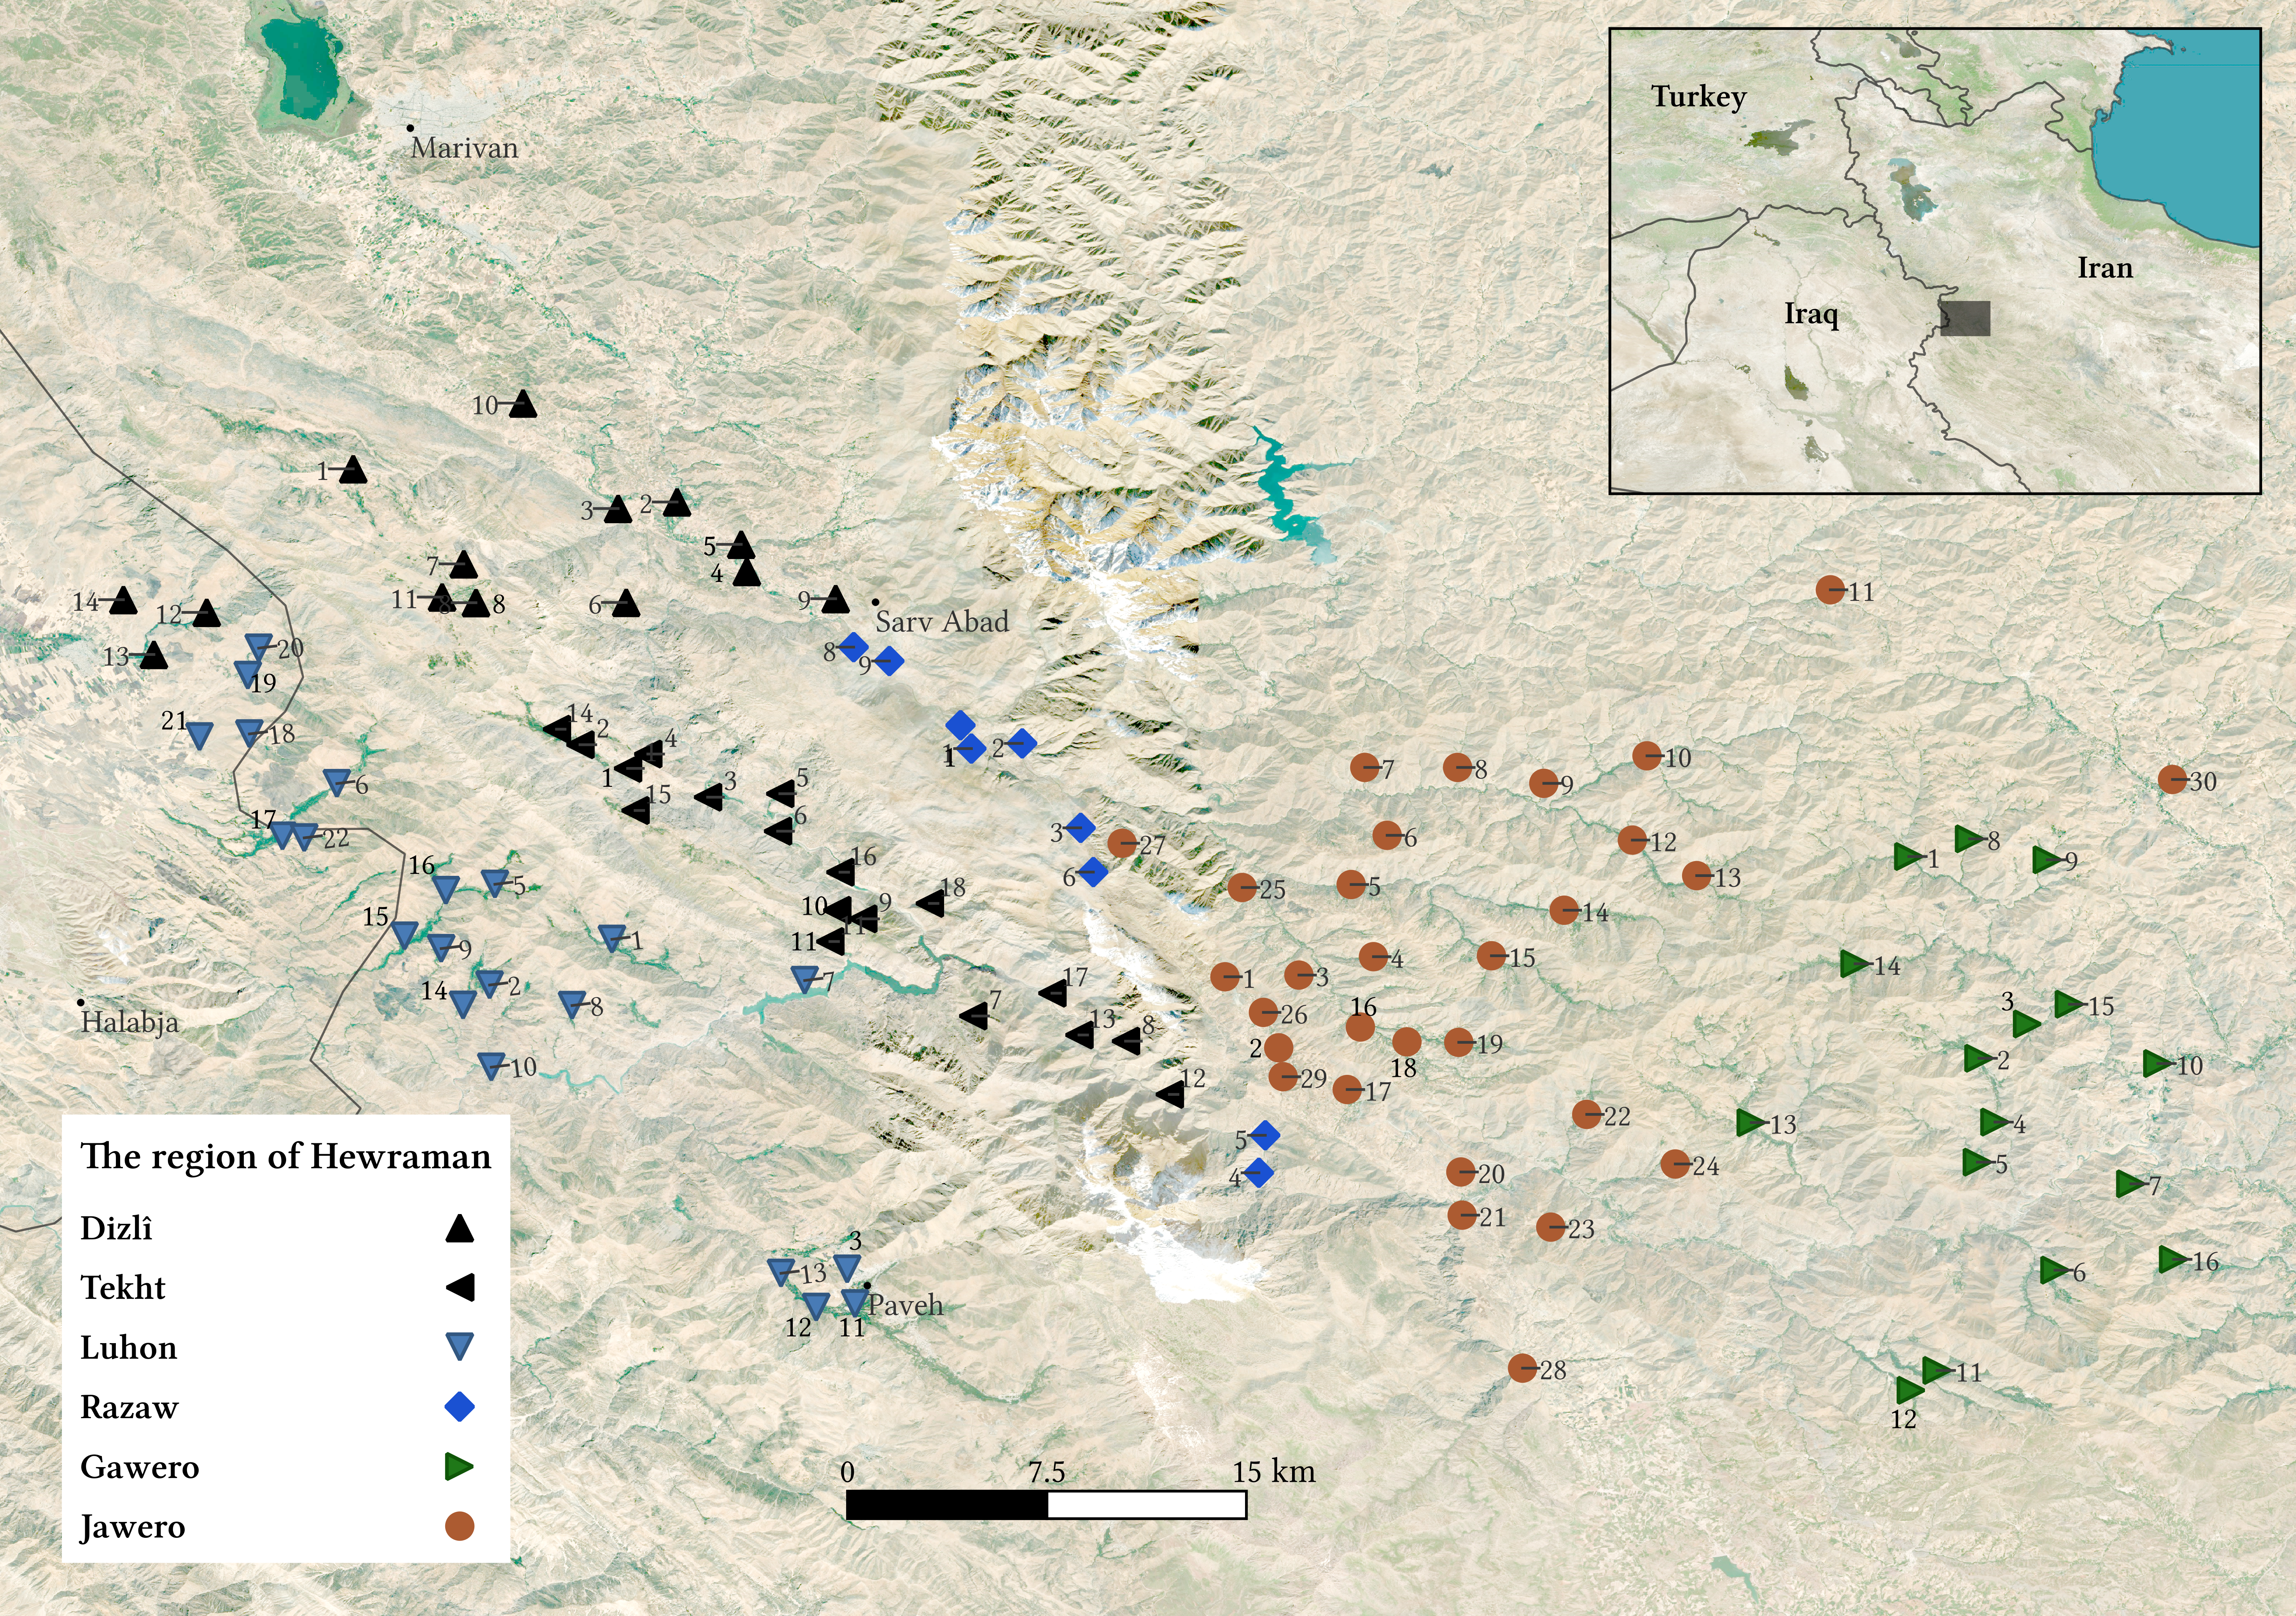
\includegraphics[width=\textwidth]{figures/Hewraman0107.png}
    \caption{The region of Hewraman and its divisions}
    \label{fig:hewmap}
    \end{figure}

There are no precise figures on the number of Hewramî\il{Hewramî} speakers. \citet{MacKenzie1987Avroman} puts the number of speakers at around 10,000. More recently, \citet{mohammadirad_language_2022} estimated the number of speakers to be about 120,000 in Kordestan province (western Iran) following a survey of linguistic distribution in the province. The population of Hewraman Tekht in the 2011 census was 2,761. The speakers refer to their language as \textit{Hewramî}, a term used by neighbouring Kurdish\il{Kurdish} speakers to refer to the Hewramî\il{Hewramî} vernacular. In addition, Hewramî\il{Hewramî}-speaking people self-identify as Kurds in a more socio-cultural and historical sense of the term Kurd, a sense which Kurds also employ to characterise Hewramî\il{Hewramî}s and Kurds alike.\footnote{See also \citet[25]{hassanpour_nationalism_1992}.} 

Although it is spoken by a small community, \citet[289]{hassanpour_nationalism_1992}{} reports that the Iranian government broadcast two-hour daily radio programmes in Hewramî\il{Hewramî} from 1977 to 1979. There was also broadcasting in Hewramî\il{Hewramî} after the Islamic revolution on Radio Sanandaj. These broadcasting programmes, however, did not result in the promotion of Hewramî\il{Hewramî}. Instead, the goal has been the political integration of the Hewramî\il{Hewramî}-speaking community. In Iraqi Kurdistan, broadcasting in Hewramî\il{Hewramî} has been boosted in recent years following the proliferation of TV channels. In neither of the sovereign states is Hewramî\il{Hewramî} promoted as an official language. More recently, the autonomous region of Iraqi Kurdistan has agreed that education be carried out in Hewramî\il{Hewramî} in localities with a significant Hewramî\il{Hewramî} population.

% and the propagation of the theory that the Hewramî community and Gorans were not Kurds
\section{The place of Hewramî\il{Hewramî} within Iranian dialectology} \label{sect:hew.ir.dialectology}
Hewramî\il{Hewramî} (ISO 639--3 hac) is a language that belongs to the Gorani\il{Gorani} language cluster of the Iranian languages (Indo-European: Iranian: Central Iranian: Northwestern Iranian: (Adharic:) Gorani\il{Gorani}: Hewramî\il{Hewramî}). 

Gorani\il{Gorani} varieties are scattered in the heart of Kurdish\il{Kurdish} parts of Iran and Iraq, shaded in Figure \ref{fig:goranidialects}. In Iran, there are Gorani\il{Gorani}-speaking communities south of the Hewraman region. The Gorani\il{Gorani} languages in Iraq are mostly placed to the west of the Hewraman region, from where they stretch as far as the Mosul plain to the north, where they are the vernacular of such communities as Kakaʼī, Šabak, Sarlī, or Bāĵaɫānī. 
\begin{figure}[htp]
    \centering
    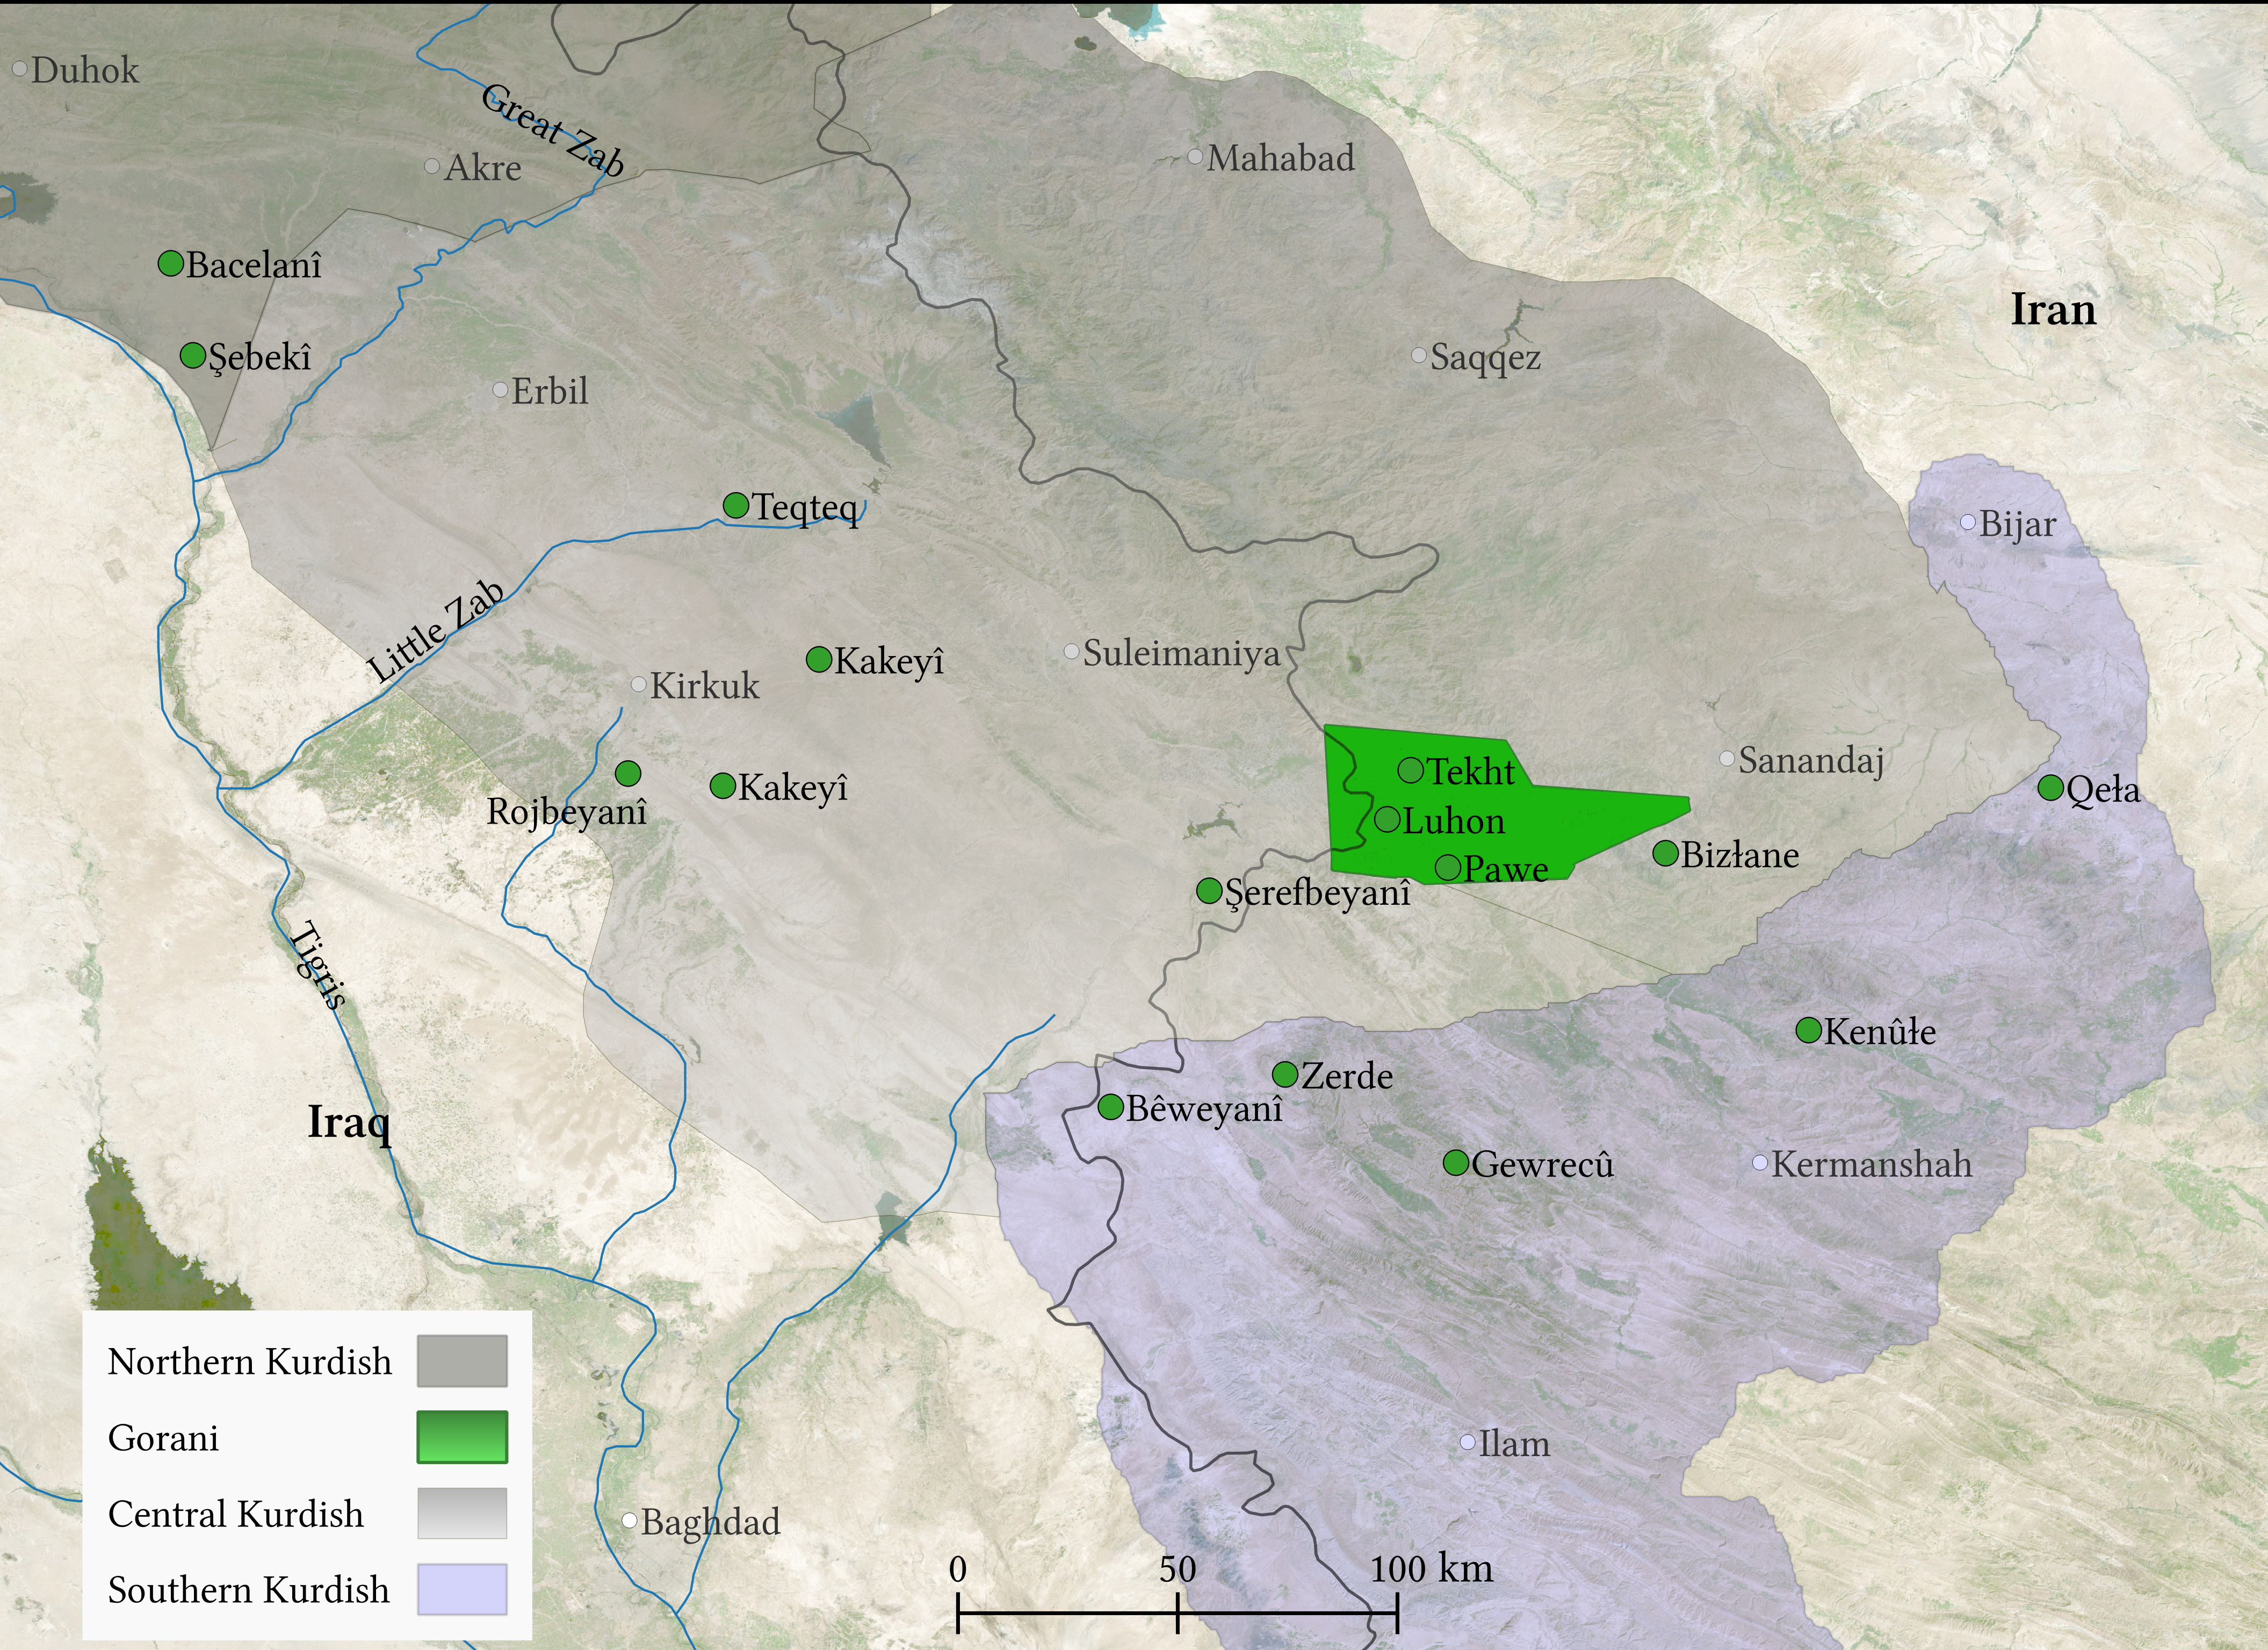
\includegraphics[width=\textwidth]{figures/Gorani dialects.png}
    \caption{Existing Gorani\il{Gorani} varieties}
    \label{fig:goranidialects}
\end{figure}

Gorani\il{Gorani} languages are characterised by preserving features dating back to the Old Iranian period. Within traditional Iranian philology, Gorani\il{Gorani} is considered a member of the Northwestern branch of Iranian languages along with Zazaki\il{Zazaki}, Taleshi\il{Taleshi}, and Kurdish\il{Kurdish}. Together with Zazaki\il{Zazaki}, Gorani\il{Gorani} varieties are shown to have preserved Northwestern phonological features par excellence \citep{paul_position_1998}.

Hewramî\il{Hewramî} is generally considered ``the best preserved and most archaic dialect" within the Gorani\il{Gorani} language cluster (see \citealt[4]{mackenzie_dialect_1966} and \citealt[]{MacKenzie1987Avroman}{}). The nominal morphology has preserved the fusional case\is{case}, gender\is{gender}, and number\is{number} affixes on nouns. In the verbal morphosyntax, ergativity is retained in verbal agreement and the nominal case marking\is{case marking}. Though note that 1st and 2nd person pronouns have lost case distinctions. Copula endings are distinguished for gender\is{gender} in the \textsc{3sg}. The progressive aspect is expressed by a constituent resembling an infinitive\is{infinitive} before the inflected form of the verb. Many of these features have been weakened or lost in the peripheral Gorani\il{Gorani} languages.

Varieties of Gorani\il{Gorani} were once spoken widely in the region. Gorani\il{Gorani} flourished as the literary language at the court of Ardalan principality (14th--19th centuries CE).\footnote{Gorani\il{Gorani} was also the court language of the neighbouring Baban principality, based in Suleimaniyya, up until the early 18th century when it was later replaced by Sorani Kurdish\il{Kurdish!Central} \citep{leezenberg_gorani_1992}.} Gorani\il{Gorani} also serves as the language of the religious texts of the heterodox Yarsan community in western Iran. 

Gorani\il{Gorani} varieties have been long in contact with vernaculars of Kurdish\il{Kurdish} and are assumed to predate Kurdish\il{Kurdish} in the region \citep{mackenzie_origins_1961}. The current distribution of varieties scattered across the Kurdish\il{Kurdish} zone gives evidence of a once-vibrant language, which gave way to Kurdish\il{Kurdish} over time (\citealt[]{mackenzie_dialect_1966}{}, \citealt[]{leezenberg_gorani_1992}{}). There are accounts of language shift to Kurdish\il{Kurdish} in some Gorani\il{Gorani} communities in the 19th and 20th centuries \citep[see][]{christensen_les_1921,kurdistani_mizgani_1930,leezenberg_gorani_1992, mahmoudveysi_meter_2016}{}{}. For example, \citet[3]{mahmoudveysi_meter_2016}{} reports that speakers of Bēwänījī, Rijābī, and Gähwāräī localities around Kerend (Iran), which were investigated by \citet[]{mann_mundarten_1930}{} as Gorani\il{Gorani} varieties, have now shifted to vernaculars of Southern Kurdish\il{Kurdish!Southern}.

 Recent scholarship has shown that the Gorani\il{Gorani} substrate within Kurdish and other local languages is most visible within the immediate Hewramî\il{Hewramî} zone of influence. \citegen{khan_language_2023} study of language contact in Sanandaj reveals that the impact of Hewramî\il{Hewramî} is far greater than Kurdish\il{Kurdish} on the Jewish Neo-Aramaic\il{Neo-Aramaic} dialect spoken there, suggesting that Hewramî\il{Hewramî} was once more widely spoken in this now dominantly Kurdish\il{Kurdish}-speaking town. A more recent study by the authors highlights the impact of Gorani\il{Gorani} on the Neo-Aramaic\il{Neo-Aramaic} dialect in Sanandaj and neighbouring Neo-Aramaic\il{Neo-Aramaic} varieties \citep{KhanMohammadirad+2024+171+198}. \citet[]{mohammadirad_gorani_nodate}{} is a case study of the Gorani\il{Gorani} substrate in the Southern varieties of Central Kurdish\il{Kurdish!Central}, e.g., CK Sanandaj, bordering the Hewramî\il{Hewramî} speech zone. In other publications, the author illustrates the Gorani\il{Gorani} substrate in the Southern varieties of Central Kurdish\il{Kurdish!Central} in the areas of bound inflectional morphology \citep[][]{mohammadirad_bound_nodate}{}{}, and word order\is{word order} \citep[][]{mohammadirad_zagros_nodate}{}{}. The picture that emerges from these most recent studies is that the morphosyntactic and phonological differences between the Northern varieties of Central Kurdish\il{Kurdish!Central} and Southern varieties of Central Kurdish\il{Kurdish!Central} can be understood by reference to a Gorani\il{Gorani}/Hewramî\il{Hewramî} substrate in the Southern varieties. 

 In recent years, a new line of scholarship has emerged that studies Gorani\il{Gorani}/Hewramî\il{Hewramî} varieties within the bigger Kurdish\il{Kurdish} dialectology e.g., \citet{opengin_pronominal_2022, mohammadirad_lenition_nodate}. The use of the term Kurdish\il{Kurdish}/Kurdic to refer to Gorani\il{Gorani}/Hewramî\il{Hewramî} varieties follows from the importance of Gorani\il{Gorani} in understanding the history of Kurdish\il{Kurdish} language and Gorani\il{Gorani} being part of Kurdish\il{Kurdish} in the larger socio-historical and cultural sense of the term Kurdish\il{Kurdish}. This latter sense is also reflected in the perceptual identity of Hewramî\il{Hewramî}/Gorani\il{Gorani} speakers. 

\section{Hewraman Tekht} \label{sect:hewramitext}
Tekht Hewramî\il{Hewramî!Tekht} is a variety of Hewramî\il{Hewramî}, spoken at the centre of the greater Hewraman region (see Figure \ref{fig:hewraman}). The term Tekht comes from the name of the region whose administrative centre is the city of Hewraman Tekht (Orāmān-e Takht). The town has a population of around 5,000. The inhabitants of the city are all Hewramî-speaking. The Hewraman region was registered as a cultural heritage by UNESCO in 2021.\footnote{\url{https : / / whc . unesco . org / en / list / 1647/}} This has led to an influx of tourists coming to the region both from within Iran and abroad and will undoubtedly have a bearing on the town's vernacular. 
\begin{figure}[htp]
    \centering
    \includegraphics[width=\textwidth]{figures/hewraman-village.jpg}
   \caption{Hewraman Tekht (photo credit: © Hamid Binaei Faa / UNESCO World Heritage Sites)}
    \label{fig:hewraman}
\end{figure}

The administrative region of Hewraman Tekht consists of 19 localities (see Figure \ref{fig:hewmap}). It is unclear if the vernacular of all these localities can be grouped under the Tekht variety, especially localities like Naw and Deɫemerz, located close to the Luhon and Jawero regions, respectively.

The inhabitants of the region are generally bilingual in Central Kurdish\il{Kurdish!Central}. This is most notably the case for men. Women over the age of 40 are usually monolingual in Hewramî\il{Hewramî}. The region's inhabitants also have some knowledge of Persian\il{Persian}, though it seems that competence in Persian\il{Persian} is higher among men than women. The situation for the younger generation is different since they all learn Persian\il{Persian} through schooling. It could be the case that the younger generation who has never left Hewraman does not speak any Kurdish\il{Kurdish} but knows Persian\il{Persian} through schooling. 

The inhabitants of Hewraman generally engage in an agropastoral lifestyle, which is semi-nomadic with vertical migration. During warm seasons, people migrate to the highlands, where they plant cereals, tend livestock, and migrate back to the lowlands during cold seasons. However, this lifestyle is waning, and the agropastoral lifestyle has given way to urbanism in Hewraman Tekht and increasingly in the surrounding villages. 

The Hewram\^i people are well known for their craftsmanship. Woodwork, stonework, and weaving shoes are still practised in Hewraman. The first two jobs are traditionally associated with men, while women generally weave shoes. The people of Hewraman traditionally engage in gardening. Mulberries and walnuts are common products in the region.

\section[The affiliation of Tekht Hewramî]{The affiliation of Tekht Hewramî\il{Hewramî!Tekht} and its status within Hewramî\il{Hewramî} dialectology} \label{sect:affiliation-hew}
Tekht Hewramî\il{Hewramî!Tekht} is one of the most conservative varieties of Hewramî. It is nearest in its morphosyntax to the Luhon variety studied by \citet{mackenzie_dialect_1966}. A general characteristic of Gorani\il{Gorani} varieties is that the more distance they are from the core mountainous Hewraman region, the less conservative they are. For instance, ergativity and nominal gender\is{gender} marking, belonging to the class of ``mature features\is{mature features}'' \citep{dahl_growth_2004}, tend to get lost in Gorani\il{Gorani} varieties outside Hewraman. 

Within Hewramî\il{Hewramî}, major varieties have notable morphosyntactic differences. While these differences await a thorough study, provisionally, the following features distinguish Tekht Hewramî\il{Hewramî!Tekht} from the neighbouring Luhon\il{Hewramî!Luhon} variety. 
The gender\is{gender} system of the two varieties exhibits some variation, as seen in the native lexicon below:

\TabPositions{2.5cm,5cm}
\ea
 Tekht H.\il{Hewramî!Tekht}\tab  Luhon H.\il{Hewramî!Luhon} \\
\textit{masaw} (\textsc{m})\tab  \textit{masawî} (\textsc{f})\tab  `fish' \\
\textit{asaw} (\textsc{m})\tab  \textit{asawî} (\textsc{f})\tab  `mill' \\
\textit{çiraw} (\textsc{m})\tab  \textit{çirawî} (\textsc{f})\tab  `lamp' \\
\z

In some loanwords\is{loanwords}, while the gender assignment\is{gender assignment} is identical, the endings differ across Tekht\il{Hewramî!Tekht} and Luhon\il{Hewramî!Luhon}. 
\TabPositions{2.5cm,5cm,8cm}
\ea
Tekht H.\il{Hewramî!Tekht}\tab  Luhon H.\il{Hewramî!Luhon} \\
\textit{hêɫeke}\tab  \textit{hêɫekî} \tab  `fine sieve' (\textsc{f}) \tab  cf. Turkish\il{Turkish} \textit{elek}\\
\z 

In nominal morphology, the two varieties differ in the use of the oblique case on past transitive subject (A-past) arguments. According to \citet[51]{mackenzie_dialect_1966}, in Luhon, the oblique case is limited to inanimate agents of past transitive verbs (A's). In Tekht, by contrast, oblique marking is additionally available for non-human animate A's (\ref{ex.animate-obl}) and human A's (\ref{ex.hum-obl}). In other words, the ergative case marking in Luhon is limited to the lowest agents in the animacy hierarchy. The Tekht variety retains an earlier stage of oblique marking on a broader range of agents, including human and non-human.
\ea 
\ea[]{
\textit{îse cawê kerdêne çêro.} \\ 
\gll îse \textbf{ caw(e)-ê} kerdê=ne çêr=o \\ 
 now road\textsc{-f.sg.obl} do\textsc{.pst.ptcp.f=cop.3sg.f:O} under\textsc{=post} \\ 
\glt `Now, the stone is laid under the road.' \hfill[ZP.53]
}
\ex[]{
\textit{marêwî gesta.} \\
\gll \textbf{mar-êw-î} gest-a \\
snake-\textsc{indf-m.sg.obl} bite.\textsc{pst-1sg:O} \\
\glt `A snake bit me.' \hfill[MP.09] \label{ex.animate-obl}
}
\ex[]{
\textit{pađşay desûriş dan be min.} \\ 
\gll \textbf{pađşa-î} desûr=iş da=n be min \\ 
 king\textsc{.m-sg.obl} order\textsc{.m=3sg:A} give\textsc{.pst.ptcp.m=cop.3sg.m:O} to \textsc{1sg} \\  
\glt `The king has ordered me [to do this].' \hfill[JP.209]\label{ex.hum-obl}
}
\z
\z

The Tekht variety\il{Hewramî!Tekht} preserves the gender\is{gender} distinction of predicative adjectives, e.g., in copula clauses. In the Luhon variety\il{Hewramî!Luhon}, by contrast, the feminine\is{feminine} form of the adjective is extended to the singular\is{singular} set. This is shown in (\ref{ex.wes.infl1}) for the inflection of \textit{weş} `well'.
\ea \label{ex.wes.infl1}
Luhon H.\il{Hewramî!Luhon}\tab  Tekht H.\il{Hewramî!Tekht} \tab   \\
 \multirow{2}{*}{\textit{weşe=na}}\tab  \textit{weş=na}\tab  `I (\textsc{m}) am well.' \\
\tab  \textit{weşe=na}\tab  `I (\textsc{f}) am well.'\\
 \multirow{2}{*}{\textit{weşe=nî}}\tab  \textit{weş=nî}\tab  `You (\textsc{m}) are well.' \\
\tab   \textit{weşe=nî}\tab  `You (\textsc{f}) are well.'\\
\z 

The two varieties exhibit differences in the stem formation of several verbs. 
\TabPositions{1.5cm,4cm,6cm,8cm}
\ea
Tekht H.\il{Hewramî!Tekht} \tab  \tab Luhon H.\il{Hewramî!Luhon}\\
\textsc{prs} \tab  \textsc{pst} \tab  \textsc{prs} \tab  \textsc{pst} \\
\textit{wen-}\tab  \textit{wena-}\tab  \textit{wan-}\tab  \textit{wana-}\tab  `read'\\
\textit{piseř-} \tab  \textit{piseřa-} \tab \textit{ seř-} \tab  \textit{seřa-} \tab  `wipe' \\
\textit{cen-}\tab  \textit{cena-}\tab  \textit{incen-}\tab  \textit{incena-} \tab  `mince' \\
\textit{biřfan-}\tab  \textit{biřfana-}\tab \textit{ řfan-}\tab  \textit{řfana-}\tab  `abduct' \\
\z 

Both varieties employ preverbal TAM prefixes (i.e., indicative and subjunctive prefixes) to a limited extent. Phonological factors condition the occurrence of these prefixes, e.g., before vowel-initial verbs in both varieties. However, Luhon H.\il{Hewramî!Luhon} tends to use these prefixes with more verbs; see (\ref{ex.ind-sbjv-difference}). For example, w-initial verbs tend to take the indicative prefix in Luhon\il{Hewramî!Luhon}, but not in Tekht\il{Hewramî!Tekht} (See \citealt[]{karim_imperfective_inreview}{, for explanation}).

\TabPositions{2.5cm,5cm}
\ea \label{ex.ind-sbjv-difference}
Tekht H.\il{Hewramî!Tekht}\tab  Luhon H.\il{Hewramî!Luhon}\\
\textit{wan-o} \tab  \textit{mi-wan-o} \tab  `he/she reads'  \\
\textit{wer-o} \tab  \textit{(mi)-wer-o} \tab  `he/she eats' \\
\textit{taw-o} \tab  \textit{mi-taw-o} \tab  `he/she can' \\
\textit{zan-o} \tab  \textit{mi-zan-o}\tab  `he/she knows' \\
\textit{\v{r}em-o} \tab  \textit{mi-\v{r}em-o}\tab  `he/she runs' \\
\z

\section{Earlier research} \label{sect:lit.gorani}

Gorani\il{Gorani} languages, among them the Hewramî\il{Hewramî} varieties especially, have long intrigued philologists and linguists alike. A first major -- and often unnoticed -- monograph-length study on a variety of Hewramî\il{Hewramî} was a descriptive grammar of Tekht Hewramî\il{Hewramî!Tekht} and the Pawe\il{Hewramî!Pawe} dialect (spoken in the northeast of Kermanshah in the city of Pawe) by \citet{christensen_les_1921}. This grammar resulted from a field trip to Sanandaj and Hewraman by Åge Meyer Benedictsen in 1901. The Hewramî\il{Hewramî} description comes from a collection of seven texts, four of which were collected from a young speaker of Ruwar dialect (P. Rūbār), whom Benedictsen met in Sanandaj. The remaining three texts were collected in Hewraman, in the village of Nawe S\^ute, which I have been unable to locate on the map. The Pawe material features one text and four poems. 

A second major work on Gorani\il{Gorani} varieties was carried out by \citet{mann_mundarten_1930}. The book contains chapter-long descriptions of eight Gorani\il{Gorani} varieties, including Kanduali, Auramani, Bajalani, Biwaniji, Gahwarai, Rijabi, Sayyidi, and Zardai. Among these, only Kandulai has been described in detail. Little grammatical description is offered for the rest of the varieties, and the respective sections consist mainly of lexicon and a few texts. The Auramani sketch deals with the linguistic analysis of proper Hewramî\il{Hewramî}, though, as \citet{mackenzie_dialect_1966} notes, it is not evident which dialect of Hewramî\il{Hewramî} is investigated here. 

The best-known grammar of Hewramî\il{Hewramî} is \citegen{mackenzie_dialect_1966} description of the Luhon\il{Hewramî!Luhon} dialect of Hewramî. The monograph is based on the speech of a single male Kurdish\il{Kurdish}-Hewramî\il{Hewramî} bilingual whom MacKenzie met in London. The grammar is detailed and remains the only reliable description of a variety of Hewramî\il{Hewramî} ever since. Nonetheless, it is brief and economical. Indeed, the book mainly covers morphology, perhaps in line with the tradition of grammar writing at the time. Less coverage has been given to phonology and especially syntax. 

In recent years, several scholars have devoted themselves to describing the most endangered varieties of Gorani\il{Gorani}, situated outside Hewraman and considered peripheral Gorani varieties. This has resulted in the publication of two sketch grammars of the peripheral Gorani varieties of Gewrecû\il{Gorani!Gewrecû} \citep{mahmoudveysi_gorani_2012} and Zerde\il{Gorani!Zerde} \citep{mahmoudveysi_gorani_2013}, spoken in western Iran. \citet{mahmoudveysi_hawrami_2018} offer a short grammatical description of the Hewramî dialect of Pawe\il{Hewramî!Pawe}. The authors have now embarked on preparing a grammatical description of the Shabaki\il{Gorani!Shabaki} dialect of Gorani spoken in the Mosul Plains.

Despite the recent rising interest in Gorani\il{Gorani} varieties, \citegen{mackenzie_dialect_1966} descriptive grammar is the only standard description of a Hewramî\il{Hewramî} variety to date. Other varieties of Hewramî\il{Hewramî} remain largely under-investigated. This book aims to provide a detailed grammatical description of the Tekht variety of Hewram\^i\il{Hewramî!Tekht}, which, as seen in \S\ref{sect:affiliation-hew}, differs in many respects from the more southern Luhon variety. The grammar is based on field recordings I collected over the course of several field trips to the Hewraman region over the past seven years. It provides a detailed account of the phonetics, phonology, morphology, syntax and lexicon of Hewramî, grounded in current linguistic methods. Despite what is often assumed, there is a high degree of dialectal variation within Hewramî\il{Hewramî} varieties. Indeed, it is unclear whether the vernaculars of Dizlî and Şamyan belong to any known three varieties of Hewramî\il{Hewramî}. Likewise, the morphosyntactic features of the Jawaro variety remain largely unknown to scholars working on Hewramî\il{Hewramî} dialectology. It is hoped that the current monograph will encourage scholars to produce comprehensive descriptions of the remaining Hewramî\il{Hewramî} varieties.

\section{Fieldwork behind this study} \label{sect:fieldwork}

The material for this book was mainly gathered during various rounds of fieldwork conducted in Hewraman Tekht between March 2016 and August 2023. I visited the region for the first time in March 2016 and conducted a pilot linguistic fieldwork. On this first field trip, my goal was mainly to get familiar with the speech community and get an idea of patterns of language use on a daily basis. I recorded spontaneous speech and dialogues, and conducted a few elicitation tasks, primarily focusing on verb conjugation. A recording I collected on this trip appears as a glossed text in \citegen[557--564]{khan_language_2023} study of language contact in Sanandaj. 

The second field trip took place in June and July 2017. This trip was conducted as part of my PhD dissertation on pronominal clitics in Western Iranian languages. During this trip, I conducted elicitation tasks using visual stimuli and a questionnaire with native speakers from Hewraman Tekht. In addition, I recorded some spontaneous spoken data and recorded a narration of the \textit{Pear story}. The elicited and spontaneous data collected in this trip formed the basis for the study of argument indexing and syntax of pronominal clitics in Tekht Hewramî\il{Hewramî!Tekht} \citep[see][365--372]{mohammadirad_pronominal_2020}{}{}, within the context of Western Iranian languages. 

The material from these two trips, additional elicited grammar surveys carried out with Hewramî\il{Hewramî} speakers, and further recordings served as the basis for the description of linguistic features of Tekht Hewramî\il{Hewramî!Tekht} in \citegen{khan_language_2023} detailed study of language contact in Sanandaj entitled: \textit{Language contact in Sanandaj: A study of the impact of Iranian on Neo-Aramaic}. The documentation of Hewramî began to take shape during the work with Geoffrey Khan on the mentioned book between 2020 and 2023.  

The linguistic material for this book comes principally from a field trip to the region in August 2022. During that field trip, which lasted three weeks, I contacted the locals in Hewramî\il{Hewramî}, which greatly facilitated fieldwork and contact with the inhabitants. I made recordings of 15 narratives. The recordings were made using a Zoom H5 Handy Recorder, which produced audio files in WAV format. I conducted my fieldwork mostly in Hewraman Tekht but also visited Serû Pîrî (a village north of Hewraman) and Benen (the summer habitat for the inhabitants of Hewraman Tekht, located in the highlands). During this fieldwork, I transcribed most of the recordings and double-checked my interpretation of recordings with my native assistant, Amir, to ensure that the correct interpretation had been achieved. In addition, I carried out many elicited grammar surveys (including a questionnaire) with Amir and, occasionally, with a few other people in Hewraman Tekht. The questionnaire was developed within the framework of the project “A Linguistic History of Minorities in the Near East” at the University of Cambridge for studying phonological, morphosyntactic, and lexical variation within Kurdic.\footnote{\url{https://www.ames.cam.ac.uk/research/project/echoes-vanishing-voices-mountains-linguistic-history-minorities-near-east}} The 15 narratives collected in this trip were transcribed and translated and later fully glossed as a text corpus volume representing Hewramî oral narratives (see \citealt{mohammadirad_speking_the_past} for details).

The fourth field trip took place in July 2023. On this trip, I mainly conducted elicitation tasks on issues I encountered while preparing a first draft of the current grammar. Additionally, I compiled the verb list presented in Appendix \ref{verb_list} and collected more recordings in Hewraman Tekht. During this trip, I collected further recordings of spontaneous speech in Hewraman Tekht, Serû Pîrî, and Bennen. This trip allowed me to travel to the nearby villages and get a first impression of linguistic diversity within the localities in which Tekht Hewramî\il{Hewramî!Tekht} is spoken. I was lucky to meet two competent storytellers in Nwên (one of whom was originally from Silên), who narrated some 25 spoken narratives characteristic of the folkloristic tradition in Hewraman. These narratives, as well as a few additional tales that I gathered in Hewraman Tekht in July 2023, constitute a collection of tales, a comprehensive processing of which is planned as a projected publication \citep{mohammadirad_folktale_inprep}. In discussing the linguistic features of Tekht Hewramî\il{Hewramî!Tekht}, I sometimes draw on the folkloristic material just discussed (see \S\ref{sect:folktale-corpus}) to back up the description of Hewramî\il{Hewramî} features. Still, the main grammatical analysis is based on the glossed text corpus in \citet{mohammadirad_speking_the_past}. 

\section{Main text corpus} \label{sect:corpus.hewrami-text}

The 15 narratives collected in August 2022 (see the previous section) comprise the main corpus behind the current book. These narratives yield a total of 96 minutes of running speech. The recordings have been time-aligned with translation using the annotation software ELAN. The recordings, along with the ELAN files, and time-aligned texts, have been archived on the open-access platform Zenodo (see \citealt{mohammadirad_2025_15419952}), and can be found at \url{https://zenodo.org/records/15419952}.

The recorded texts belong to different supposed genres: folktales, local anecdotes, myths, oral history of the region, and autobiographies. The resulting texts form the Tekht Hewramî\il{Hewramî!Tekht} database and are a touchstone for the grammatical description and lexicon. The text corpus behind this study has been entirely glossed in FLEx, from which the glossed texts were converted into the specific formatting for linguistic examples required by Language Science Press in \LaTeX, using a Python script. The glossaries at the end of the book were drawn from the TeX file using additional Python scripts. 

The narrators who recounted the narratives were all over 60 years old at the time of recording. In many ways, then, this descriptive grammar is indicative of the language as spoken by the older generation. Nonetheless, in a few cases, the grammar highlights the generational difference in language use. As for the linguistic profile of the narrators, except for the narrator of the text JE, who is a monolingual, the rest exhibit some bilingualism in Kurdish\il{Kurdish}. These speakers have a weak bilingualism pattern, with Hewramî\il{Hewramî} as their dominant language and Kurdish\il{Kurdish} as less dominant. In addition, some of these narrators showed weak competence in Persian\il{Persian}.

\begin{table}[t]
\caption{The main text corpus \citep[]{mohammadirad_speking_the_past}}
\label{tab:texts}
    \centering
    \small
\begin{tabularx}{\textwidth}{QlQr}
    \lsptoprule
       \textsc{title} & \textsc{id} &\textsc{topic} \\
	\midrule
		\textit{zaroɫe û bizê} `The baby and the goat' & ZB & Local anecdote/myth about an abandoned baby  \\
       \textit{zaroɫe û qiřolû darî} `The baby and the tree hollow' & ZQ &Local anecdote/myth about an abandoned baby  \\
       \textit{herbene} `The donkey keeper' & HB & Local anecdote/myth about a talking donkey \\
        \textit{peɫê merekuř} `A swarm of grasshoppers' & PM  &Local anecdote/myth, grasshoppers \\
        \textit{derde gulî} `Leprosy' & DG & Local anecdote/myth about a man suffering from leprosy \\
        \textit{Şêx ʕumer û Cafir san} `Sheikh Omar and Jafir San' & ŞC & Local anecdote about recent history  \\
        \textit{duwê padşε} `Two kings' & DP  & Oral history, two kings claiming Hewraman \\
        \textit{jîwayû Pîr Şelîyarî} `Pir Shaliyar’s life' & JP  & Oral history, hagiography  \\
        \textit{zemawinew Pîr Şalîyarî} `Pir Shaliyar’s wedding' & ZP & Oral history, hagiography \\
        \textit{babaw Pîr Şalîyarî} `Pir Shaliyar’s grandfather' & BP & Oral history, hagiography \\
        \textit{kuřû şuwaney} `The shepherd’s son' & KŞ  & Folktale \\
        \textit{jîwayû Heyasî} `Hayas’s life' & JH  & Folktale \\
        \textit{řisûmatû ewsayma} `Our past traditions' & RE & Recollections of traditional life \\
        \textit{jîwayû ewsayma} `Our past life'  & JE & Recollections of traditional life, autobiography \\
       \textit{jîwayû min} `My life'  & JM  & autobiography \\
    \lspbottomrule
\end{tabularx}
\end{table}


The 15 narratives consist of approximately 10,000 words. Table \ref{tab:texts} lists the titles of the texts and their identifier codes in \citegen[]{mohammadirad_speking_the_past} volume. The examples taken from the latter volume are cited in the grammar using the initials of the texts along with an identifier number corresponding to the numbered annotation units--typically a sentence or a clause. For instance, ZB.20 corresponds to sentence number 20 in the ZB text. This guides the readers to the larger linguistic context from which the examples are taken.


There are some glossing and translation conventions worthy of noice. Object language examples are presented in two versions, an orthographic one that corresponds to actual surface realisations, and the morphologically segmented version, which contains representations of the morphemes that are closer to their assumed underlying forms. Example (\ref{ex.awunderlyin}) illustrates how the surface form \textit{awekê} `the water' in the orthographic version can be segmented at the underlying representation, while the second line in example (\ref{ex.kisunderlyin}) illustrates the underlying analysis for \textit{winû} `blood of' and \textit{kîseɫê} `tortoise (\textsc{f.sg.obl})' in the orthographic version. 

\ea \label{ex.awunderlyin} 
\textit{awekê biřo.} \\ 
\gll aw(î)-ekê biř-o \\ 
 water\textsc{.f-def.f.sg} cut\textsc{.prs.ind-3sg:A} \\ 
\glt `He cut off the water supply.' \hfill[DP.34]
\z 

\ea \label{ex.kisunderlyin}
\textit{winû kîseɫê sawî be...} \\ 
\gll win(î)-û kîseɫ(î)-ê s\'aw-î be \\
 blood\textsc{.f-ez.gen} tortoise\textsc{.f-obl.f} rub\textsc{.prs.sbjv-2sg:A} to \\ 
\glt `You may rub tortoise's blood on ...'  \hfill[DG.47]
\z 

A feature of Hewramî narratives is the frequent use of the present tense as the narrative tense to recount past events (see \S\ref{sect:narrativeprs}). Consequently, all the tales and narratives in \citet[]{mohammadirad_speking_the_past,mohammadirad_folktale_inprep} --- which are the source for linguistic examples in the current book --- have been translated into the past tense, including in cases where the narrative present is used to describe past time events (see \ref{ex.awunderlyin} for an example). Readers are encouraged to keep this in mind when interpreting the examples. 

In the translation of linguistic examples, square brackets indicate words and meanings that are implicit or not stated in the text, while round brackets clarify the reference of participants in the text, see \REF{ex.trans}.

\newpage
\ea \label{ex.trans}
\textit{maço, `nezanam.'}\\ 
\gll m-aç-o ne-zana=m\\ 
 \textsc{ind-}say\textsc{.prs-3sg:A} \textsc{neg-}know\textsc{.pst=1sg:A}\\ 
\glt `He (the man) said, `I didn't understand [his point].' \hfill[JH.26]
\z 

\section{Folktale corpus} \label{sect:folktale-corpus}
As briefly discussed in \S\ref{sect:corpus.hewrami-text}, the morphosyntactic description of Hewramî\il{Hewramî} is further backed up by additional folktales which I gathered at Nwên and Hewraman Tekht in August 2023. These folktales provide a rich source for studying the folkloristic tradition of Hewraman. Once fully processed, they will be published as a collection of folktales from Hewraman. For the current grammar, I have occasionally included example sentences from these tales in the main text. All the examples in the book from the folktale collection come with the initials of the tales and an identifier number, which refers to the place where the examples have been cited within the mentioned tale.

The folktale collection consists of 31 tales, totalling around 25,000 words. Here, it suffices to name each narrative with its initials, with a detailed description awaiting a projected publication of these tales \citep{mohammadirad_folktale_inprep}. \\
\\
1. \textit{mûsa û řuwase} (MR) `Moses and the fox' \\
2. \textit{mama mama} (MM) `Mama mama' \\
3. \textit{pîrejenî û kitê} (PK) `The old woman and the cat' \\
4. \textit{dêđê û çwar kinaçê} (ÇK) `The stepmother and four girls' \\
5. \textit{jenê fêlebaze} (JF) `A cunning wife' \\
6. \textit{jenî û lîrewireş} (JL) `The woman and the lira-seller' \\
7. \textit{wiɫkɫe} (WL) `Wilkle' \\
8. \textit{hacî û jenekêş} (JC) `Haji and his wife' \\
9. \textit{şaw mara û şaw melekuřa} (ŞŞ) `The king of snakes and the king of grasshoppers' \\
10. \textit{jenî û ħewt weywê} (HW) `A woman and seven daughters-in-law' \\
11. \textit{patşa û pîrî} (PP) `The king and the old man' \\
12. \textit{kuře keçeɫe} (KK) `The bald boy' \\
13. \textit{hêyasî jîr} (HJ) `Heyas the Wise' \\
14. \textit{siɫtan mehmûđ û heyasî jîr} (SH) `Sultan Mahmoud and Heyas the Wise' \\
15. \textit{meɫik ehmeđ} (ME) `Malek Ahmad' \\
16. \textit{Kinaçêw Taɫî meẍrêbî} (KT) `The daughter of Tal from Maghreb' \\
17. \textit{mar û peyxwmer} (MP) `The snake and the Prophet' \\
18. \textit{meɫa yoso û meɫa xiđir} (YX) `Mullah Yoso and Mullah Khidr' \\
19. \textit{şê bayzîdî boystamî} (BB) `Sheikh Bayzid Bostami' \\
20. \textit{çil paɫewanê û hezretû ʕelî} (ÇH) `Forty warriors and His Highness Ali' \\
21. \textit{pađşa û wezîr} (PW) `The king and the vizier' \\
22. \textit{duwê birayê} (DB) `Two brothers' \\
23. \textit{meɫa xiđir û şûwane} (XŞ) `Mullah Khidr and the shepherd' \\
24. \textit{xiđre xuɫekêş} (XX) `Khidr the Soil Carrier' \\
25. \textit{ehmeđe dize} (ED) `Ahmad the Thief' \\
26. \textit{şa ʕebas} (ŞE) `Shah Abbas' \\
27. \textit{sîyawehş û keyxesrew} (SK) `Siyawahsh and Keykhosrow' \\
28. \textit{hezretû mûsay û fêrʕon} (MF) `Moses and Pharaoh' \\
29. \textit{hacî mehmûđ û řozgarya} (HM) `Haji Mahmoud and the Rozgaris' \\
30. \textit{bêjen û menîje} (BM) `Bezhan and Manizha' \\
31. \textit{heyas û siɫtan mehmûyî} (HS) `Heyas and Sultan Mahmoud' \\


\end{sloppypar}

\chapter{Typological overview} \label{ch.typology}
This chapter lays out the major typological features of Tekht Hewram\^i\il{Hewramî!Tekht}. This should provide readers with a first-hand touch on the language, though the coverage of features remains concise and eclectic. Defining grammatical properties of Hewramî includes a primary phonological gender assignment system, split-ergative alignment, two-term case system, differential argument flagging, differential argument indexing, disharmonic SOV order, phonemic stress placement, and a complex deictic system. 
\begin{sloppypar}

\section{Phonology}
The consonant inventory includes 29 consonant phonemes, four of which are peripheral phonemes occurring in a few loanwords\is{loanwords} or limited in their distribution within the syllable or word. These are represented in parentheses in Table \ref{tab:Cchart_typological-overview}. 
\begin{table}
\caption{Consonant phonemes}
\label{tab:Cchart_typological-overview}\small
\fittable{\begin{tabular}{@{}llllllllll@{}}
		\lsptoprule
&{Labial} & {Lab.-dent.} & {Alv.} & {Postalv.} & {Pal.} & {Vel.} & {Uv.} & {Phar.} & {Glott.} \\
\midrule

{Stop} & p b &  & t  d &  &  & k  ɡ& q &  & (ʔ) \\
{Affricate} &  &  &  & t͡ʃ  d͡ʒ &  &  &  &  & \\
{Nasal} &\phantom{0 }m &  &\phantom{0 }n &  &  &\phantom{0 }(ŋ)  &  &  & \\
{Fricative} &  & f  & s  z & ʃ      ʒ &  & x    (γ) &   & ħ  ʕ & h \\
{Tap} &  &  &\phantom{0 }ɾ &  &  &  &  &  & \\
{Trill} &  &  &\phantom{0 }r &  &  &  &  &  & \\
{Lateral} &  &  &\phantom{0 }l (ɫ)& &  &  &  &  & \\
{Approx.} &\phantom{0 }w &  &         &  &\phantom{0 }j &  & & & \\
\lspbottomrule
	\end{tabular}
	}
\end{table}%

The vowel inventory consists of nine phonemic vowels: four front vowels <î> /i/, <ê> /e/, <ɛ> /ɛ/, <e> [ɛ${\sim}$æ]; three back vowels <û> /u/, <o> /o/, <a> /ɑ/; and two central vowels <i> /ɨ/ and <u> /ʊ/. Of these, /i, e, ɛ, u, ɑ, o/ and [ɛ${\sim}$æ] are long vowels, while /ɨ/ and /ʊ/ are short. The vowel phonemes are distinguished by height and backness, as well as by their phonetic realisation (see \S\ref{phonetic-realisation}). 
\begin{figure}
    \includegraphics[width=.60\textwidth]{figures/vowel_qualityn.png}
    \caption{Hewramî\il{Hewramî} vowel inventory}
    \label{Hewrami-vowels}
\end{figure}

A syllable in Hewramî\il{Hewramî} consists minimally of a vowel and maximally of a vowel flanked by two consonants, yielding (C)(C)V(C)(C). Consonant clusters in the syllable structure are broken up by the epenthetic vowels \textit{i} and \textit{u}, depending on the quality of the adjacent consonants.

Hewramî\il{Hewramî} is a language with predictable stress placement. Masculine\is{masculine} nouns follow what may be considered the general rule of word-final stress placement, whereas feminine\is{feminine} nouns generally have penultimate stress (except nouns ending in \stackunder[-10pt]{\^{e}}{\'{}}). Similarly, in past tense verbal categories, the stress is penultimate. 
Hewramî\il{Hewramî} is a language with phonemic stress\is{phonemic stress} placement: for most verbs, stress is the only mechanism to distinguish between subjunctive and indicative moods in present tense verbs. Figure \ref{fig:bero_ind-typ} and \ref{fig:bero_sbjv-typ} exhibit different stress patterns associated with the verbs \textit{ber\'o} `he/she takes' and \textit{b\'ero} `that he/she takes'. For each verb, the higher intensity peak highlights the stressed vowel.
\begin{figure}[htb]
  \begin{subfigure}[b]{0.5\textwidth}
    \includegraphics[width=\textwidth]{figures/text_bero_he_takes.png}
    \caption{Indicative `he/she takes'}
    \label{fig:bero_ind-typ}
  \end{subfigure}\begin{subfigure}[b]{0.5\textwidth}
    \includegraphics[width=\textwidth]{figures/text_bero_that_he_takes.png}
    \caption{Subjunctive `that he/she takes'}
    \label{fig:bero_sbjv-typ}
  \end{subfigure}
  \caption{The stress position for the verb `he takes'}
\end{figure}

The most important morphophonemic processes are metathesis\is{metathesis} and assimilation\is{assimilation}. Many disyllabic loans from Arabic containing a pharyngeal consonant in the coda of the second syllable are subject to metathesis\is{metathesis}, illustrated in (\ref{ex.metathesis.1}). The metathesis\is{metathesis} occurs following the restriction against the rise of sonority across syllable boundaries \citep{gouskova_falling_2001}.
\TabPositions{2cm,5cm,7.5cm}
\ea \label{ex.metathesis.1}
\textit{seʕbe}\tab  [ˈsæʕ.bɛ]\tab  cf. Ar.\il{Arabic} \textit{sabāħ}\tab  `morning’ \\
\textit{weʕze}\tab  [ˈwæʕ.zɛ]\tab  cf. Ar.\il{Arabic} \textit{wazʕ}\tab  `situation’ \\
\textit{cuʕme}\tab  [d͡ʒʊħ.ˈmɛ]\tab  cf. Ar.\il{Arabic} \textit{jomʕa}\tab  `Friday’ \\
\z

The assimilation\is{assimilation} processes, both progressive\is{progressive assimilation} and regressive\is{regressive assimilation}, have the effect of creating geminate consonants. Total progressive assimilation\is{progressive assimilation} is seen in \textit{çinne} where /d/ fully assimilates to the preceding nasal sound. On the other hand, \textit{kulle} features total regressive assimilation with /ř/ in \textit{kuř} assimilating to the following lateral phoneme.
\ea
\textit{çinne}\tab  `how much’\tab  < *\textit{çinde}\tab  cf. CK.\il{Kurdish!Central} \textit{çende} \\
\textit{kulle}\tab  `small boy’\tab  < *\textit{kuřle}\\
\z

\section{Morphology}
Hewramî\il{Hewramî} morphology is largely concatenative, though some fusional patterns are attested. Nouns are morphologically marked for case\is{case}, number\is{number}, and gender\is{gender}. These categories are expressed by fusional inflectional affixes on the noun. All three represent a two-way distinction: singular\is{singular} and plural\is{plural} for number\is{number}, masculine\is{masculine} and feminine\is{feminine} for gender\is{gender} (only in the singular\is{singular}), and \textsc{direct}\is{direct case} and \textsc{oblique}\is{oblique case} for case\is{case}. Direct\is{direct case} and oblique\is{oblique case} are Iranian-internal terms roughly equivalent to `nominative' and `non-nominative' cases, respectively. 

 There is one underlying nominal inflectional class in Tekht Hewramî\il{Hewramî!Tekht}. The inflection of a noun is predictable from the phonological shape of the base and from its gender. The underlying fusional suffixes are included in Table \ref{tab:nom-infl-under1}.

\begin{table}
    \begin{tabular}{lllllll} 
    \lsptoprule
& \textsc{sg.dir}& \textsc{sg.obl}& \textsc{pl.dir} & \textsc{pl.obl} \\
\midrule
\textsc{m}& {-\O}& \textit{-î} & \multirow{2}{*}{\textit{-ê}}& \multirow{2}{*}{\textit{-a}} \\
\textsc{f}& {-\O}& \textit{-ê} & & \\
\lspbottomrule
\end{tabular}
    \caption{Nominal inflectional suffixes--underlying forms}
    \label{tab:nom-infl-under1}
\end{table}

The oblique case\is{oblique case} is a continuation of the functions expressed by old non-nominative case endings. It expresses, among other things, direct objects of present tense verbs, transitive subjects of past tense verbs, possessors, and complements of prepositions. The direct case\is{direct case} expresses intransitive subjects, transitive subjects of verbs derived from the present stem, and direct objects of past tense verbs (see \S\ref{case-section}). 

Nouns are overtly marked for the category of gender\is{gender}. Hewramî\il{Hewramî} has two genders, masculine\is{masculine} and feminine\is{feminine}. Gender\is{gender} is assigned to nouns primarily based on the ending the nouns take. Nouns which in their citation form end in a consonant or stressed \textit{-é}, \textit{-\stackunder[-10pt]{\^{i}}{\'{}}}, \textit{-\stackunder[-10pt]{\^{u}}{\'{}}}, and \textit{-ó} are masculine\is{masculine}. In addition, a subset of nouns ending in stressed \textit{-á }are masculine\is{masculine}. On the other hand, nouns ending in \textit{-ê} (whether stressed or not) and those ending in unstressed \textit{-e} and \textit{-î}, are feminine\is{feminine}. The class of feminine\is{feminine} nouns also includes a subset in stressed \textit{-á}. In other words, the language has a phonological gender assignment system (according to the typology in \citealt{corbett_gender_1991}). It is notable that semantic and morphological factors also have a role in gender assignment\is{gender assignment} (see \S\ref{gendersection}). 

Case distinctions\is{case distinction} are lost in the speech act pronouns\is{speech act pronouns}. Third-person pronouns mark case\is{case} and gender\is{gender} distinctions in the singular\is{singular} and case distinctions\is{case distinction} in the plural\is{plural} (see Table \ref{tab:case-pronouns}). 

\begin{table}
    \begin{tabular}{llcl}
    \lsptoprule
 &  \textsc{dir}& \textsc{obl}\\
\midrule
\textsc{1sg}& \multicolumn{2}{c}{\textit{min}} \\
\textsc{2sg}& \multicolumn{2}{c}{\textit{to}} \\
\textsc{3sg.m}&\textit{ađ}&\textit{ađî} \\
\textsc{3sg.f}& \textit{ađe}& \textit{ađê}\\
\textsc{1pl}& \multicolumn{2}{c}{\textit{ême}} \\
\textsc{2pl}& \multicolumn{2}{c}{\textit{êşme}} \\
\textsc{3pl}& \textit{ađê}&\textit{ ađîşa} \\
\lspbottomrule
    \end{tabular}
    \caption{Case distinctions\is{case distinction} in pronouns}
    \label{tab:case-pronouns}
\end{table}

Gender\is{gender} is a morphosyntactic category in Hewramî\il{Hewramî} since it is involved in agreement. At the level of noun phrases, agreement in gender\is{gender agreement} can be found on (i) adjectives and (ii) definite suffixes\is{definite suffix}. At the clause level, agreement targets for the category of gender\is{gender agreement} are predicative adjectives, \textsc{3sg} copula markers (\textsc{3sg.m} \textit{꞊n/ ꞊a}; \textsc{3sg.f} \textit{꞊ne}), and \textsc{3sg} inflectional person suffixes in past stem verbs (\textsc{3sg.m} \textit{-∅}; \textsc{3sg.f} \textit{-e}) (see \S\ref{sect:gend-agreement}). In (\ref{agr-adj}), the predicative adjective, the participle, and the \textsc{3sg} copula agree with the \is{gender agreement} topicalised NP in gender:

\newpage
\ea
\textit{î dega toş vînî çoɫe bîyêne.} \\ 
\gll î dega to=ş vîn-î çoɫ-\textbf{e} \textbf{bîyê=ne} \\ 
 \textsc{dem.prox} village{\textsc{.f}} \textsc{2sg=3sg:O} see\textsc{.prs.ind-2sg:A} deserted-\textsc{f} be\textsc{.pst.ptcp.f=cop.3sg.f:S} \\ 
\glt `This village, which you see, was deserted.' \hfill [JE.4] \label{agr-adj}
\z

Similarly, number\is{number} is a morphosyntactic category in Hewramî\il{Hewramî}. Typical agreeing elements for the category of number\is{number agreement} are adjectives and some classifiers\is{classifier} (see \S\ref{Number-section}). 
\ea
\textit{yerê danê hêɫê} \\ 
\gll yerê dan(e)-ê hêɫ(e)-ê \\ 
 three \textsc{clf}\textsc{.pl} egg\textsc{.m}\textsc{-pl.dir} \\ 
\glt `three eggs' \hfill [JH.81] 
\z

Adjectives feature gender\is{gender agreement} and number agreement\is{number agreement} with head nouns when used attributively and predicatively. When substantivised, adjectives inflect for case\is{case} as well. In light verb constructions\is{light verb constructions}, the adjective complement of a light verb\is{light verb} carries number\is{number agreement} and gender agreement\is{gender agreement} with S and O. In (\ref{ex.lv-agr-1}), the predicate is \textit{neweş kewtey} `fall ill'. In (\ref{ex.lv-agr-2}), the predicate is \textit{zamdar kerđey} `injure'. In both predicates, the adjective complement exhibits agreement with clausal arguments.
\ea 
\textit{kinaçêw padşaw misrî neweşe gino.} \\ 
\gll kinaçê-û padşa-û misr-î neweş-\textbf{e} gin-o \\ 
daughter\textsc{.f.dir-ez.gen} king\textsc{.m-ez.gen} \textsc{pn-m.sg.obl} ill\textsc{-f} fall\textsc{.prs.ind-3sg:S} \\  
\glt `The king of Egypt’s daughter fell sick.' \hfill [ZP.25] \label{ex.lv-agr-1}
\z 

\ea
\textit{ême zamdarê nekero} \\
\gll ême zamdar-\textbf{ê} ne-ker-o \\
\textsc{1pl} wounded\textsc{-pl} \textsc{neg.sbjv-}do\textsc{.prs-3sg:A} \\ 
\glt `He should not injure us.’ \hfill [DG.64] \label{ex.lv-agr-2}
\z 

As a reflection of it being spoken in a high mountainous area, Hewramî\il{Hewramî} features a complicated demonstrative system. In addition to the third person forms in Table \ref{tab:case-pronouns}, which are unmarked anaphoric pronouns, the language has two sets of anaphoric demonstratives\is{anaphoric demonstratives}, distinguished based on distance, and two sets of demonstrative pronouns. 

\begin{table}
    \begin{tabular}{lllll}
 \lsptoprule
 \multicolumn{3}{c}{Proximal} & \multicolumn{2}{c}{Distal} \\
& \textsc{dir}& \textsc{obl} & \textsc{dir}& \textsc{obl} \\ 
\midrule
\textsc{m}&\textit{îđ} &\textit{îđî} &\textit{ew} &\textit{ewî}\\
\textsc{f}& \textit{îđ(e)}& \textit{îđê}& \textit{ewe}& \textit{ewê} \\
\textsc{pl}& \textit{îđê}& \textit{îđîşa} & \textit{ewê, ewêşa}& \textit{ewîşa} \\
 \lspbottomrule
    \end{tabular}
    \caption{Anaphoric demonstratives}
    \label{tab:anaphoricpronouns}
\end{table}

\begin{table}
    \begin{tabular}{lllll}
 \lsptoprule
\multicolumn{3}{c}{Proximal} & \multicolumn{2}{c}{Distal} \\
& \textsc{dir}& \textsc{obl} & \textsc{dir}& \textsc{obl} \\ 
\midrule
\textsc{m}&\textit{îne} &\textit{îney} &\textit{ane, ûne} &\textit{aney} \\
\textsc{f}& \textit{îne, înî}& \textit{înê}& \textit{anê}& \textit{ane} \\
\textsc{pl}& \textit{înê, înî}& \textit{îna, înîşa}& \textit{anê}& \textit{ana, anîşa} \\
 \lspbottomrule
    \end{tabular}
    \caption{Demonstrative pronouns}
    \label{tab:demonstative pronouns}
\end{table}

The different sets of third-person pronouns express diverse, sometimes overlapping, functions. Unmarked anaphoric pronouns track participants that are established as topics. Anaphoric demonstratives\is{anaphoric demonstratives} may reactivate a referent that has occurred with some distance in the previous discourse. They are also used to establish new discourse topics (see \S\ref{sect:3perspronouns}). The choice between unmarked personal pronouns and anaphoric demonstratives\is{anaphoric demonstratives} is evident in the following excerpt. The former tracks an already-established topic. The latter expresses a topic shift and new information.
\ea 
\textit{mila ew kuřekey yoyşa bera. aneşa zilterû ʕalter bo ađî bera. ewî minya qiřoɫû darêwe.} \\ 
\gll mi-l-a ew kuř-ekey yo-î=şa ber-a ane=şa zil-ter=û ʕal-ter b-o \textbf{ađî} ber-a \textbf{ewî} mi-ny(e)-a qiřoɫ-û dar-êwe \\ 
\textsc{ind-}go\textsc{.prs-3pl:S} \textsc{dem.dist} son\textsc{.m-def.m.sg.obl} one\textsc{.m-sg.obl=3pl:PSR} take\textsc{.prs.ind-3pl:A} \textsc{dem.dist.m.3sg.dir=3pl:PSR} big\textsc{-cmpr}=and good\textsc{-cmpr} be\textsc{.prs.ind-3sg:S} \textsc{3sg.obl.m} take\textsc{.prs.ind-3pl:A} \textsc{3sg.obl.m} \textsc{ind-}put\textsc{.prs-3pl:A} hollow\textsc{.m-ez.gen} tree\textsc{.m-indf}\\ 
\glt `They went away [and took] that son. They took one of them (i.e., of the boys), the one who was bigger and healthier; they took \textbf{him}. They left \textbf{him (i.e., the other one)} in the hole in the tree.' \hfill [ZB.40]--[ZB.41]
\z 

The demonstrative pronouns can have exophoric use, anaphoric use, discourse presentative use, and emphatic use (see \S\ref{sect:ind-dem-pro}). Local adverbial demonstratives\is{local adverbial demonstratives} distinguish between visible from the deictic centre and invisible from the deictic centre (see \S\ref{sect:loc-adv-dem}). 

Nouns are marked for definiteness\is{definiteness} by way of the suffixes \textit{-eke} and \textit{-e}. The former inflects for gender\is{gender}, case\is{case}, and number\is{number}. Unlike known definiteness\is{definiteness} systems, the definite suffix\is{definite suffix} is not used with all nouns with identifiable referents. Rather, once a noun has been identified with a definite status, it is no longer necessary to mark it by the definite suffix. This means that bare nouns\is{bare noun} can have a definite reading. In the following excerpt, \textit{kinaçê} has a definite reference by virtue of its appearance with the demonstrative \textit{î}. In the continuation of the discourse, the same referent occurs in its bare\is{bare} form. 
\ea
\ea[]{ 
\textit{be mezebû wêşa î kinaçeşa pey nîkah kerew. narîşo!} \\ 
\gll be mezeb-û wê=şa \textbf{î} \textbf{kinaç(ê)=e}=şa pey nîkah k\'er-e=û n(e)-ar-î=ş=o \\ 
by religion\textsc{-ez.gen} \textsc{refl=3pl:PSR} \textsc{dem.prox} girl\textsc{.f=dem=3pl:R} to marriage\textsc{.m} do\textsc{.prs.imp-2sg:A}{=and} \textsc{neg.sbjv-}bring\textsc{.prs-2sg:A=3sg:O=compl} \\  
\glt `Marry the girl to him according to [the customs of] their religion. May you not bring her back!' \hfill [JP.165]
}
 
\ex[]{ 
\textit{lalo gino gelû kinaçê.} \\ 
\gll lalo gin-o gel-û \textbf{kinaçê} \\ 
maternal\_uncle\textsc{.m} fall\textsc{.prs.ind-3sg:S} with\textsc{-ez.gen} girl\textsc{.f} \\ 
\glt `The uncle set off on the road with the girl.' \hfill [JP.166]
}
\z 
\z 

The simple verb has two verbal forms divided into \textsc{present} and \textsc{past} stems. The two-stem system is divided into two tense-based categories roughly equivalent to present and past tenses. The most productive tool for forming new verbs is light verb constructions\is{light verb constructions} consisting of a light verb\is{light verb} and a non-verbal element. \\
Verbs inflect for the morphological and morphosyntactic features of number\is{number}, person, gender\is{gender} (only in \textsc{3sg}, in verbs derived from past stem), tense, mood, and aspect. Verbal categories are built by present and past stems combined with inflectional person suffixes and modal prefixes. Table \ref{tab:my_label} exemplifies the inflection of the suppletive verb \textit{witey} `sleep' in \textsc{1sg} across different TAM forms. 
\begin{table}
    \fittable{%
    \begin{tabular}{lll}
\lsptoprule
Present indicative\is{present indicative}& \textit{m-ûs-û}& [\textsc{ind}-sleep.\textsc{prs-1sg:S}] \\
Present subjunctive\is{present subjunctive}& \textit{b-ûs-û}&[\textsc{sbjv}-sleep.\textsc{prs-1sg:S}] \\
Present progressive\is{present progressive}& \textit{m-ûs-ay m-ûs-û}&[\textsc{ind}-sleep.\textsc{prs-nmlz} \textsc{ind}-go.\textsc{prs-1sg:S}] \\
Past progressive\is{past progressive}& \textit{wis-ay wis-ên-a}&[sleep.\textsc{prs-nmlz} go.\textsc{prs-aug-1sg:S}] \\
Habitual past\is{habitual past} & \textit{wis-ên-a}&[sleep.\textsc{prs-aug-1sg:S}] \\
Irrealis past\is{irrealis past}& \textit{wis-ên-a}&[sleep.\textsc{prs-aug-1sg:S}] \\
\\
Past perfective\is{past perfective}& \textit{wit-a}& [sleep.\textsc{pst-1sg:S}] \\
Past conditional& \textit{wit-εn-ê}&[sleep.\textsc{pst-cond.aug-1sg:S}] \\
Perfect\is{perfect} & \textit{wite=na}&[sleep.\textsc{pst.ptcp.m=cop.1sg:S}] \\
Perfect progressive\is{perfect progressive}& \textit{wit-î wite=na}&[sleep.\textsc{pst-nmlz} sleep.\textsc{pst.ptcp.m=cop.1sg:S}] \\
Irrealis perfect\is{irrealis perfect}& \textit{wite=b-û}&[sleep.\textsc{pst.ptcp.m}=be\textsc{.prs-1sg:S}] \\
Conditional perfect\is{conditional perfect}& \textit{wite=bî-{ɛ}n-ê}&[sleep\textsc{.pst.ptcp}=be.\textsc{pst-cond.aug-1sg:S}] \\
Past perfect\is{past perfect}& \textit{wite=b-ên-ê}&[sleep.\textsc{pst.ptcp.m}=be\textsc{-aug-1sg:S}] \\
Perfect pluperfect\is{perfect pluperfect}& \textit{wite=bîye=na}&[sleep.\textsc{pst.ptcp.m}=be.\textsc{pst.ptcp.m=cop.1sg:S}]\\
\lspbottomrule
    \end{tabular}}
    \caption{The inflection of \textit{witey} `sleep' in \textsc{1sg} across different TAM categories}
    \label{tab:my_label}
\end{table}

The verb forms with present-time reference fall broadly into four classes. In all verb classes, the negation of the indicative is identical to the prohibitive, as opposed to the negation of the subjunctive. Class 1 features the majority of verbs, as exemplified by the verb \textit{berđey} `take'. Here, indicative, subjunctive, and imperative verb forms are prefix-less. The verbs beginning with \textit{m} in this class exceptionally have the prohibitive prefix \textit{ne-}. Class 2 is specific to verbs with a C(V) structure, with the exception of \textit{bîyey} `be, become' (\textsc{prs} \textit{b-}; \textsc{pst} \textit{bî-}), which belongs to class 1. The verb forms in this class regularly take the TAM prefixes, except the imperative prefix is occasionally dropped. Class 3 is limited to low-vowel-initial verbs, with the negative prefixes for both the indicative and prohibitive being \textit{nime-}, unlike the verbs in classes 1 and 2. Class 4 is limited to high back-vowel and mid-vowel-initial verbs. Like the verbs in class 3, the verb forms in this class feature vowel coalescence of the TAM prefixes with the stem. However, unlike in class 3, the verb forms in class 4 use the negation forms \textit{m\'e-}. An exception is the verb \textit{êşay} `to hurt', for which the negative of the indicative can be expressed by either \textit{m\'e-} or \textit{nim\'e-} (see \S\ref{section-vinfmorph}).

\begin{table}[hbt!]

    \begin{tabular}{rllccc}
        \lsptoprule
 
&& & \textsc{ind} & \textsc{sbjv} & \textsc{imp/proh} \\
   \midrule
\multirow{2}{*}{1} & \multirow{2}{*}{\textit{ber-} `take'} & \textsc{aff} & \textit{ber-\stackunder[-10pt]{\^{i}}{\'{}}} & \textit{b\'er-\^i} & \textit{b\'er-e} \\
&& \textsc{neg} & \textit{m\'e-ber-\^i} & \textit{n\'e-ber-\^i} & \textit{m\'e-ber-e} \\
\midrule
\multirow{2}{*}{2} & \multirow{2}{*}{\textit{de-} `give'} & \textsc{aff} & \textit{mi-đe-\stackunder[-10pt]{\^{i}}{\'{}}} & \textit{bi-đ\'e-\^i} & \textit{(bi)-đ(e)-\'e} \\
&& \textsc{neg} & \textit{m\'e-đe-\^i} & \textit{n\'e-đe-\^i} & \textit{m\'e-đ(e)-e} \\
\midrule
\multirow{2}{*}{3} & \multirow{2}{*}{\textit{az-} `let'} & \textsc{aff} & \textit{m-az-\stackunder[-10pt]{\^{i}}{\'{}}} & \textit{b-\'az-\^i} & \textit{b-\'az-e} \\
&& \textsc{neg} & \textit{nim(e)-\'az-\^i} & \textit{n-\'az-\^i} & \textit{nim(e)-\'az-e} \\
\midrule
\multirow{2}{*}{4} & \multirow{2}{*}{\textit{ûs-} `sleep'} & \textsc{aff} & \textit{m-\^us-\stackunder[-10pt]{\^{i}}{\'{}}} & \textit{b-\stackunder[-10pt]{\^{u}}{\'{}}s-\^i} & \textit{b-\stackunder[-10pt]{\^{u}}{\'{}}s-e} \\
&& \textsc{neg} & \textit{m\'e-ws-\^i} & \textit{n\'e-ws-\^i}  & \textit{m\'e-ws-e} \\
    \lspbottomrule
    \end{tabular}
    \caption{Verb classes with present time reference, inflected in \textsc{2sg} }
    \label{tab:text_me}
\end{table}
Hewramî\il{Hewramî} has a mixed adpositional typology, which reflects its structure being affected by both OV languages like Turkish\il{Turkish}, and VO languages like Arabic\il{Arabic}, and Aramaic\il{Aramaic} \citep{stilo_circumpositions_2009}. Additionally, adpositions exhibit applicative-like properties when taking pronominal arguments (see \S\ref{sect:absolute_prep}). Example:
\ea 
\textit{xway ketê pey kîyasen.} \\ 
\gll xwa-î ket-ê \textbf{pey} kîyase=\textbf{n} \\ 
God\textsc{.m-sg.obl} bed\textsc{-indf} to send\textsc{.pst.ptcp.m=cop.3sg.m:R} \\ 
\glt `[As if] God had sent him a bed.' \hfill [JP.69]
\z

\section{Syntax}
The basic order of modifiers within the NP is DEM NUM N ADJ POSS, exemplified in (\ref{ex.np.structure}). Hewramî\il{Hewramî} uses two different head linkers in the structure of the NP, dubbed ezafe/ezafeh in Iranian linguistics, depending on the category of the modifier: \textit{-î} marks attributive ezafe\is{attributive ezafe}, whereas \textit{-û} marks genitive ezafe\is{genitive ezafe}. Additionally, an \textit{ezafe compound} \textit{-e} is used in the language with tightly-knit compound NPS, e.g. \textit{nan-e taz(e)-êwe} [bread\textsc{.m-ez.cmpd} fresh-\textsc{indf}] `a fresh [loaf of] bread'.
\ea 
\textit{a duwe ku\v{r}e ʕalew emîrî} \\ 
\gll a duwe ku\v{r}-e ʕal-e-û emîr-î \\ 
\textsc{dem.dist} two son.\textsc{ez.cmpd} good-\textsc{def-ez.gen} \textsc{pn-m.sg.obl}\\ 
\glt `those two good sons of Emir' \label{ex.np.structure}
\z 

Case marking\is{case marking} and ezafe marking interact in the structure of the noun phrase. When two possessors follow the head noun, only one formative is retained. In the following example, the expected construction would be \textit{qefesû sîne-y-û minne} [cage\textsc{.m-ez.gen} chest\textsc{.m-sg.obl-ez.gen} \textsc{1sg=post}]. However, in competition for the slot on the first possessor, only the oblique\is{oblique case} suffix remains, and the ezafe gets deleted.
\ea 
\textit{qefesû sîney minne} \\ 
\gll qefes-û sîne-\textbf{y} min=ne \\ 
 cage\textsc{.m-ez.gen} chest\textsc{.m-sg.obl} \textsc{1sg=post} \\ 
\glt `in my chest [lit. in the cage of my chest]' \hfill [DP.38]
\z 

\subsection{Word order\is{word order}}
Hewramî\il{Hewramî} has a default SOV order. This ordering is characterised by the subject not carrying the nuclear stress. The immediate pre-verbal slot is associated with the basic place of the focus\is{focus} in the clause, illustrated in (\ref{ex.sov1a}). Occasionally, the subject constituent comes between the verb and its direct object (\ref{ex.sov1typ}). This typically occurs when the subject constituent is in focus\is{focus}. The focality of the A argument in past constructions can trigger the absence of indexing of the A argument on the verb (see \S\ref{sect:damtyp}).
\ea 
\textit{çêrhur zaroɫeke şot wero.} \\ 
\gll çêr=hur zaroɫe-(e)ke şot wer-o \\ 
under\textsc{=post} child\textsc{-def.m.sg.dir} milk\textsc{.m} eat\textsc{.prs.ind-3sg:A} \\ 
\glt `The baby drank [its] milk from below.' \hfill [ZB.45]  \label{ex.sov1a}
\z

\ea
\textit{heywane awê berde.} \\ 
\gll heywane aw\stackunder[-10pt]{\^{e}}{\`{}} berd-e \\ 
 animal\textsc{.f.sg.dir} water\textsc{f.sg.obl} take\textsc{.pst-3sg.f:O} \\ 
\glt `The flood [lit. water] took away the animals.' \hfill[ZB.21] \label{ex.sov1typ}
\z

Post-verbal objects are rare. If they occur at all, they are limited to nominals with definite reference evoked in the previous discourse. They seem to be limited to certain clause types, e.g., interrogatives (\ref{ex.VO1a}) and imperatives (\ref{ex.VO2a}). 
\ea 
\textit{maça, `şanat tomeke?’} \\ 
\gll m-aç-a şana=t tom-eke \\ 
\textsc{ind-}say\textsc{.prs-3pl:A} scatter\textsc{.pst.3sg:O=2sg:A} seed\textsc{-def.m.sg.dir}\\ 
\glt `They would say, ‘Did you plant the seeds?’' \hfill [JP.39] \label{ex.VO1a}
\z 

\ea 
\textit{mekojdê a kabray!} \\
\gll me-koj-dê a kabra-î \\
\textsc{proh-}kill.\textsc{prs-2pl:A} \textsc{dem.dist} fellow\textsc{-m.sg.obl} \\
\glt `Do not kill that man!' \hfill [SH.268] \label{ex.VO2a}
\z 

Despite having OV order, Hewramî\il{Hewramî} exhibits several head-initial configurations, including Noun-Adjective, Possessed-Possessor, Matrix clauses-complement clause, Verb-Goal, and Verb-Recipient\is{recipient}, running against the predictions of head-directionality hypothesis \citep[]{dryer_greenbergian_1992}{}. 

As for non-core arguments\is{oblique arguments}, goals of verbs of motion (\ref{ex.goal2a}), recipients (\ref{ex.rec1typ}), and addressees (\ref{ex.add1typ}) are overwhelmingly realised in the post-verbal position, representing \citegen{hawkins_ordering_2008} SOVX type, where X is the non-core argument. Though note that \citet{hawkins_ordering_2008} uses the notation `X' to refer to all kinds of non-core arguments, including also comitatives, instrumentals, place, etc. These latter arguments tend to be realised pre-predicatively in Hewramî.
\ea 
\textit{êtir milo law ađî.} \\ 
\gll êtir mi-l-o \textbf{la-û} \textbf{ađî} \\ 
\textsc{disc.ptcl} \textsc{ind-}go\textsc{.prs-3sg:S} to\textsc{-ez.gen} \textsc{3sg.obl.m} \\ 
\glt `Anyhow, he went to him.' \hfill [JP.13] \label{ex.goal2a}
\z 

\ea 
\textit{nanîç miđa to.} \\ 
\gll nan=îç mi-đ(e)-a \textbf{to} \\ 
bread\textsc{.m=add} \textsc{ind-}give\textsc{.prs-3pl:A} \textsc{2sg} \\ 
\glt `They will give you a meal.' \hfill [HB.40] \label{ex.rec1typ}
\z 

\ea 
\textit{maço be xanî.} \\ 
\gll m-aç-o \textbf{be} \textbf{xan-î} \\ 
 \textsc{ind-}say\textsc{.prs}\textsc{-3sg:A} to chief\textsc{.m-sg.obl} \\ 
\glt `He said to the chief.' \hfill [KŞ.97] \label{ex.add1typ}
\z 

\subsection{Alignment\is{alignment}} \label{sect:alignment}
Hewramî\il{Hewramî} features a tense-based split ergative system both in verbal argument indexing and argument case marking\is{case marking}. The alignment\is{alignment} system is nominative-accusative for verbs derived from the present tense and ergative-absolutive for verbs derived from the past stem, though note that ergative alignment is most consistently evident in the pattern of argument indexing. This system of tense-sensitive alignment\is{tense-sensitive alignment} depends not on the transitivity of the clause in a semantic sense but on the lexical transitivity of individual verbs. That is, a verb is lexically specified as either transitive or intransitive, and that will determine how it inflects in TAM constructions based on the past stem of the verb. Whether a verb has an overt object or not is irrelevant.

In terms of verbal argument indexing, Hewramî uses verbal affix person markers to index A and S in verbs derived from the present stem, while O is expressed via person clitics. The indexing of S and A is obligatory, whereas the indexing of O is contingent on the absence of the coreferent nominal.
\ea 
\textit{milo.} \\ 
\gll mi-l-\textbf{o} \\ 
\textsc{ind-}go\textsc{.prs-\textbf{3sg:S}} \\ 
\glt `It (a tortoise) went.' \hfill [DG.61]
\z 

\ea 
\textit{beroş.} \\ 
\gll ber-\textbf{o=ş} \\ 
 take\textsc{.prs.ind-\textbf{3sg:A=3sg:O}} \\ 
\glt `He took him.' \hfill [DG.17]
\z 

In verbs derived from the past stem, O and S are indexed by verbal affixes (or copula person endings in perfect tenses), whereas clitic pronouns index the A argument. Only indexing of S is obligatory. O-indexing (see \S\ref{sect:DOI}) and A-indexing (see \S\ref{sect:differential-A-indexing}) are nearly obliqgatory. 
\ea 
\textit{amaymê.} \\ 
\gll ama-\textbf{îmê} \\ 
 come\textsc{.pst-\textbf{1pl:S}} \\ 
\glt `We came.' 
\z 

\ea 
\textit{berđîmêşa.} \\ 
\gll berđ-\textbf{îmê=şa} \\ 
take\textsc{.pst-\textbf{1pl:O=3pl:A}} \\ 
\glt `They took us.'
\z 

In terms of case marking\is{case marking}, in clauses where the verb is derived from the present stem, S (\ref{ex.align:s.prs}) and A (\ref{ex.align:A.prs}) are marked in the direct case\is{direct case}, whereas O (\ref{ex.align:o.prs}) is marked in the oblique case\is{oblique case}. 
\ea
\textit{seʕbê wiɫaxdarê mila.} \\
\gll seʕbê \textbf{wiɫaxdar-ê} mi-l-a \\
morning\textsc{.f.sg.obl} stableman-\textsc{pl.dir} \textsc{ind}-go.\textsc{prs-3pl:S} \\
\glt `In the morning, the horse grooms went.’ \hfill [ŞC.66]  \label{ex.align:s.prs} 
\z 

\ea 
\textit{îse dêwê xeber zana} \\ 
\gll îse \textbf{dêw-ê} xeber z\'an-a \\ 
 now ogre-\textsc{pl.dir} news know\textsc{.prs.sbjv-3pl:A} \\ 
\glt `If the ogres find out [about you] now' \hfill [SK.100] \label{ex.align:A.prs} 
\z 

\ea 
\textit{yewayç bero.} \\ 
\gll \textbf{yew(e)-a}=îç {} ber-o \\ 
 barley\textsc{.f-pl.obl=add} {} take\textsc{.prs.ind-3sg:A} \\ 
\glt `He took the barley seeds, too.' \hfill [JP.29] \label{ex.align:o.prs} 
\z   

In clauses with verbs derived from the past stem, S (\ref{ex.align:s.pst}) and O (\ref{ex.align:o.pst}) are marked in the direct case\is{direct case}, whereas A (\ref{ex.align:A.pst}) is marked in the oblique case\is{oblique case}.
\ea 
\textit{karewanîyê amêyanê serere.} \\ 
\gll \textbf{karewanî-ê} amêya=nê sere=re. \\ 
 caravan\_people-\textsc{pl.dir} come\textsc{.pst.ptcp.pl=cop.3sg.pl:S} top=\textsc{postp} \\  
\glt `Some passers-by had stayed there.' \hfill[DB.15]\label{ex.align:s.pst}
\z 

\ea
\textit{hewarêşa wişkin{ɛ}nê.} \\ 
\gll \textbf{hewar-ê}=şa wişkin{ɛ}=nê \\ 
 summer\_habitat\textsc{.m-pl.dir=3pl:A} scour\textsc{.pst.ptcp.pl=cop.3pl:O} \\ 
\glt `They scoured the summer habitats [searching for food etc.].' \hfill [JE.3] \label{ex.align:o.pst}
\z

\ea 
\textit{ênne paɫewana zorşa kerđen} \\ 
\gll ênne \textbf{paɫewan-a} zor=şa kerđe=n\\
so\_much warrior-\textsc{pl.obl} pressure=\textsc{3pl:A} do\textsc{.pst.ptcp.m=cop.3sg:O} \\ 
\glt `The warriors put much pressure [on the skin]' \hfill [SK.132] \label{ex.align:A.pst}
\z 
\subsection{Grammatical relations}
\subsubsection{Differential A indexing\is{differential subject indexing}} \label{sect:damtyp}
Hewramî\il{Hewramî} features tense-sensitive indexing of the transitive subject A argument: in clauses based on the present stem of the verb, verbal person/number suffixes index the A argument, whereas in clauses derived from the past stem of the verb, the historical clitic pronouns index the A argument. Unlike the verbal affixes, the clitic pronouns indexing the A-past argument are mobile. Furthermore, while indexation of A-\textsc{prs} through inflectional suffixes is obligatory, the person clitics indexing A-past arguments are sometimes missing. They may be, at least partially, in complementary distribution with an overt oblique case-marked\is{oblique case} A argument. In (\ref{ex.damintro1a}), the oblique-marked\is{oblique case} A \textit{pad\c{s}a} is the sole way to express the A argument. In (\ref{ex.damintro1b}), the \textsc{3sg} clitic \textit{=i\c{s}}, resumes the coreferent absent A argument.   
\ea
\ea[]{
\textit{min taze padşay kerdena wekêɫ.} \\ 
\gll min taze \textbf{padşa-î} kerde=na wekêɫ \\ 
\textsc{1sg} anyway king\textsc{.m-sg.obl} do\textsc{.pst.ptcp.m=cop.1sg:O} advocate\textsc{.m} \\ 
\glt `I—the king has put me in charge.' \hfill[ZP.107] \label{ex.damintro1a}
}
 
\ex[]{
\textit{watenîçiş, mişyo neberûşo.} \\ 
\gll wate=n=îç=\textbf{iş} mişyo ne-ber-û=ş=o \\ 
say\textsc{.pst.ptcp.m=cop.3sg.m:O=add=3sg:A} \textsc{aux} \textsc{neg.sbjv-}take\textsc{.prs-1sg:A=3sg:O=compl} \\ 
\glt `He (the king) has said [to me], “You shall not take her back.’'' \label{ex.damintro1b} \\ \hfill[ZP.108] 
}
\z
\z 

This optional indexing of A-past arguments is triggered by the A argument displaying properties related to focus\is{focus} \citep{MohammadiradinreviewAindx}. A focused A argument in Hewramî\il{Hewramî} can be in non-contrastive or constrastive focus. The non-contrastive focus is further divided into wh-focus\is{wh-focus focus} and completive focus\is{completive focus} (see \S\ref{sect:arginx.pst}). By way of example, in (\ref{ex.dai1}), the A argument has nuclear focus, and the A-indexing person clitic \textit{=ş} is missing:
\ea
\textit{î zeře çermeme kê berden eçêge?} \\
\gll î zeře çerme=m=e \textbf{k\stackunder[-10pt]{\^{e}}{\`{}}} berde=n eçêge \\
\textsc{dem.prox} money-\textsc{ez.cmpd} white\textsc{=1sg:PSR=deic} who take.\textsc{pst.ptcp.m=cop.3sg.m:O} here \\
\glt `\textbf{Who} has taken my white money [that is now] here?' \hfill [PK.29] \label{ex.dai1}
\z 

When the A argument is in completive focus\is{completive focus}, it is not indexed via mobile person clitics. In (\ref{ex.completive-focus1}), in response to the wh-question, the focused \textsc{2sg} A argument is not indexed. 
\ea 
\textit{maço `miɫk ehmeđ! î dijmenême kê kuştênê? to kuştênê!?'} \\
\gll m-aç-o miɫk ehmeđ î dijmen-ê-m=e \textbf{k\stackunder[-10pt]{\^{e}}{\`{}}} kuştê=nê \textbf{t\`o} kuştê=nê \\
\textsc{ind}-say.\textsc{prs-3sg:A} \textsc{pn} \textsc{pn} \textsc{dem.prox} enemy\textsc{-pl.dir=1sg=deic} who kill\textsc{.pst.ptcp.pl=cop.3pl:O} \textsc{2sg} kill\textsc{.pst.ptcp.pl=cop.3pl:O} \\
\glt `He (the king) said, Oh Milk Ahmad! \textbf{Who} has killed my enemies? \textbf{You} have killed them!?' \hfill [ME.150] \label{ex.completive-focus1}
\z 

By contrast, when the oblique-marked\is{oblique case} A NP is in the topic position and not focused, the person clitic resumes it. This explains the co-occurrence of the subject indexing clitic and the oblique-marked A argument in (\ref{ex.daiindex1}). Similarly, oblique-marked\is{oblique case} A argument in the post-verbal position co-occurs with the co-indexing person clitic (\ref{ex.daiindex2}). The clitic indexing here follows from the fact that the topical A argument is placed in the non-focal post-verbal position as an afterthought. 
\ea 
\textit{î pîyay tawaş î kinaçêşe kerde be qerarê weşeş kerdewe...} \\ 
\gll î pîya-î \textbf{taw\`a}=ş î kinaçê=ş=e kerd-e be qerar-ê weş-e=ş kerd-e=we\\ 
 \textsc{dem.prox} man\textsc{.m-sg.obl} can\textsc{.pst=3sg:A} \textsc{dem.prox} girl\textsc{.f.sg=3sg:A=dem} do\textsc{.pst-3sg.f:O} to settlement\textsc{-indf} well\textsc{-f=3sg:A} do\textsc{.pst-3sg.f:O=compl} \\  
\glt `[And if] the man has been \textbf{able} to cure the girl...' \hfill [ZP.45] \label{ex.daiindex1}
\z 

\ea 
\textit{qotê aman. asawekeş bînan qotekey.} \\
\gll qot(e)-ê ama=n asaw-eke=\textbf{ş} bîna=n \textbf{qot-ekey} \\
box-\textsc{indf} come.\textsc{pst.ptcp.m=cop.3sg.m:S} mill\textsc{.m-def=3sg} block.\textsc{pst.ptcp.m=cop.3sg.m:O} box-\textsc{def.obl.m} \\
\glt `A box came [floating on the water]. The box blocked the (water) mill.'\label{ex.daiindex2} \\\hfill [MF.75]--[MF.76] 
\z

\subsubsection{Differential P indexing}
As seen in \S\ref{sect:alignment}, P arguments are indexed by clitic pronouns in present tense constructions but via inflectional person/number suffixes in past transitive constructions. Here, differential P indexing\is{differential object indexing} means a deviation from the canonical ergative construction whereby the object is not indexed on the verb. Verbal affixes are obligatory indexes of direct objects in canonical ergative constructions, illustrated by the following example. 
\ea
\textit{to minit quɫ kerđaw.} \\
\gll to \textbf{min}=it quɫ kerđ-\textbf{a}=û \\
\textsc{2sg} \textsc{1sg=2sg:A} pierced do.\textsc{pst-1sg:O=}and \\
\glt `You disabled me.' \hfill [PW.30]
\z 

In clauses with OAV order, the verb tends to agree with the topical O. 
\ea 
\textit{werêsekê min warđêne.} \\
\gll werês(e)-ekê min warđê=ne \\
rope-\textsc{def.f.sg} \textsc{1sg} eat.\textsc{pst.ptcp.f=cop.3sg.f:O} \\
\glt `[The lion said], `I have eaten the rope.’' \hfill [ÇH.85]
\z

The expected P indexing is sometimes absent with inanimate Ps that are plural\is{plural}. In the following examples, the verb has a default \textsc{3sg.m} inflection and does not agree with the plural\is{plural} object. 
\ea 
\textit{penc çemçêşa nîyanre.} \\ 
\gll penc çemç(e)-ê=şa nîya=n=re \\ 
five spoon\textsc{.m-pl.dir=3pl:A} put\textsc{.pst.ptcp.m=cop.3sg.m:O=povb} \\  
\glt `They (my family) had set five spoons [on the tablecloth].' \hfill [JE.46]
\z 

\ea 
\textit{ewêş nîya biraw wêş.}\\
\gll ewê=ş nîya bira-û wê=ş\\
\textsc{3pl.dir=3sg:A} put\textsc{.pst.3sg.m} brother\textsc{.gen.ez} \textsc{reflx=3sg:PSR}\\
\glt `He made them (the ogres) his brothers.' \hfill[ME.99]
\z 

O-past indexing may also be absent due to affix co-optation by a higher-ranked argument in terms of animacy. In the following example, the expected \textsc{3pl} O-agreement suffix is absent on the verb because its slot has been taken over by the \textsc{3sg} suffix indexing the oblique argument\is{oblique argument}.  
\ea
\textit{kîyast sênze danê heserê\c{s}a da pene.} \\
\gll kîyast sênze danê heser(e)-ê=\c{s}a da-{\O} pene \\
 send\textsc{.pst} thirteen \textsc{clf.pl} mule\textsc{.f-pl.dir=3pl:A} give.\textsc{pst-3sg:R} to \\
\glt `He [the king] sent [his men]. They [his men] gave him (Imam Ali) thirteen mules.' \hfill [ÇH.69]  
\z 

\subsubsection{Differential A flagging\is{differential A flagging}}
The alignment\is{alignment} system licenses case marking\is{case marking} for A arguments. In TAM constructions derived from the present stem of the verb, A is marked in the direct case\is{direct case}, realised as a zero suffix in the singular\is{singular} and -\textit{ê} in the plural\is{plural}. By contrast, in verbal categories derived from the past stem of the verb, the A argument should be, by default, accompanied by the oblique case\is{oblique case} suffixes. The split alignment\is{split alignment} is only relevant for third-person nouns and pronouns. Speech act pronouns\is{speech act pronouns} have lost the case distinction\is{case distinction} (see \S\ref{tab:case-pronouns}). The following example illustrates the oblique case\is{oblique case} marking on the A-past argument.
\ea 
\textit{cafir sanî fermawan, `lodê!'} \\ 
\gll cafir san-î fermawa=n lo-dê \\ 
 \textsc{pn} \textsc{pn-m.sg.obl} say\textsc{.pst.ptcp.m=cop.3sg.m:O} go.\textsc{prs.imp-2pl:S} \\ 
\glt `Jafir San said, `Go [and bring him]!’' \hfill [ŞC.36]
\z 

In reality, not all A-past arguments are oblique-marked\is{oblique case}. A token frequency count of overt As reveals that a quarter of the third person As are not oblique-marked\is{oblique case} (see \S\ref{sect:DAM}). The data suggest that information prominence triggers oblique case marking\is{oblique case} on A-past arguments. The latter operates at two levels: ``local'' and ``global'' \citep[]{chappell2019optional}. In Hewramî\il{Hewramî}, the former is generally associated with oblique\is{oblique case} marking and the latter with direct case\is{direct case} marking. ``Local'' prominence is associated with the A argument being in narrow focus\is{narrow focus} and contrastive focus\is{contrastive focus}. In (\ref{ex2}), the case marking\is{case marking} on \textit{her} `donkey' is triggered by its contrast with \textit{min}.
\ea 
\textit{î her-î zûwaniş zana min hîçim nezanan.} \\
\gll î \textbf{her-î} zûwan=iş zana-{\O} min hîç=im ne-zana=n \\ 
 \textsc{dem.prox} donkey\textsc{-sg.obl.m} language\textsc{.m.sg.dir=3sg:A} know\textsc{.pst-3sg.m:O} \textsc{1sg} nothing\textsc{=1sg:A} \textsc{neg-}know\textsc{.pst.ptcp.m=cop.3sg.m:O} \\ 
\glt `The donkey knew the [Sheikh’s] language; I didn’t know a thing!' \label{ex2} \\ \hfill [HB.71] 
\z 

Case marking\is{case marking} on the A argument can also be triggered by global prominence. According to \citegen{mcgregor2006focal} ``expected actor principle'', in episodes of discourse with an expected actor, the actor can be left unmarked after its introduction. Any deviation from the expected actor is marked in the ergative case. One of the factors conditioning differential subject marking\is{differential subject marking} seems to be topic continuity. In the following excerpt, the established direct-marked topic of the intransitive clause in (\ref{ex.dam-pro1a}), is repeated with the transitive clause in (\ref{ex.dam-pro1b}), even though the oblique\is{oblique case} form \textit{ađîşa} is expected with the latter clause. 
\ea
\ea[]{ 
\textit{tenya ađê luw{ɛ}nê.} \\ 
\gll tenya \textbf{ađê}\textsubscript{i} luw{ɛ}=nê \\ 
 only \textsc{3pl.dir} go\textsc{.pst.ptcp.pl=cop.3pl:S} \\  
\glt `Only they\textsubscript{i} (Baba Khwada, Hama the Invisible, and Little Hama) went [to Iraq].'  \label{ex.dam-pro1a}
 }
 \ex[]{
\textit{êtir ađê watenşa, `ême diruwê meyeymê.} \\ 
\gll êtir \textbf{ađê}\textsubscript{i} wate=n=şa ême diruwê me-de-îmê \\ 
 \textsc{disc.ptcl} \textsc{3pl.dir} say\textsc{.pst.ptcp.m=cop.3sg.m:O=3pl:A} \textsc{1pl} lie\textsc{.f} \textsc{neg.ind-}give\textsc{.prs-1pl:A} \\ 
\glt `They\textsubscript{i} said, ‘We are not going to lie." \label{ex.dam-pro1b} \hfill [BP.116]--[BP.117]
}
\z 
\z 

In terms of information structure, non-oblique marked overt A-past arguments tend not to carry the nuclear stress. In other words, they behave like topics and contain given information (see \S\ref{sect:DAM} for discussion).

\subsubsection{Differential P flagging}
Direct objects in clauses based on present stem verbs exhibit differential P flagging\is{differential P flagging}. The basic pattern is that direct objects which are definite-marked (\ref{ex.def-obl}), proper nouns (\ref{ex.human-obl}), inanimate direct objects with definite reading (\ref{ex.def-obl-inanim}), and direct objects modified by demonstrative pronouns (\ref{ex.def-obl-dem}) are marked in the oblique case\is{oblique case}. 
\ea 
\textit{zeřekey bere.} \\ 
\gll \textbf{zeř-ekey} b\'er-e \\ 
 money\textsc{.m-def.m.sg.obl} take\textsc{.prs.imp-2sg:A} \\  
\glt `Take the money.' \hfill [JP.104] \label{ex.def-obl}
\z 

\ea
\textit{hêyasî bizindê!} \\
\gll \textbf{hêyas-î} bi-zin-dê \\
\textsc{pn-m.sg.obl} \textsc{imp}-take\_out\textsc{.prs-2pl:A} \\
\glt `Throw Heyas out!' \hfill [HS.15]  \label{ex.human-obl}
\z 

\ea 
\textit{muxteserû kelamî, yaney yozawe.} \\ 
\gll muxteser-û kelam-î \textbf{yane-î} yoz-a=we \\ 
 summary\textsc{.m-ez.gen} speech\textsc{-m.sg.obl} house\textsc{.m-sg.obl} find\textsc{.prs.ind-3pl:A=compl} \\ 
\glt `To cut a long story short [lit. gist of speech], they found the house.' \label{ex.def-obl-inanim} \\\hfill[JP.205] 
\z 

\ea 
\textit{a esbî zînî kere peym.} \\ 
\gll \textbf{a} \textbf{esb-î} zînî k\'er-e pey=m \\ 
 \textsc{dem.dist} horse\textsc{-m.sg.obl} saddle do\textsc{.prs.imp-2sg:A} for\textsc{=1sg:R} \\  
\glt `Saddle up the horse for me.' \hfill [ŞC.52] \label{ex.def-obl-dem}
\z 

Similarly, nouns whose referents have been mentioned in the previous discourse tend to carry case marking\is{case marking}. In the following example, the case marking\is{case marking} on \textit{yewe} is triggered by its referent being evoked in previous discourse. 
\ea 
\textit{werû mecbûrî yewayç bero.} \\ 
\gll wer-û mecbûrî-(î) \textbf{yew(e)-a}=îç {} ber-o \\ 
 out\_of\textsc{-ez.gen} obligation\textsc{-m.sg.obl} barley\textsc{.f-pl.obl=add} {} take\textsc{.prs.ind-3sg:A} \\ 
\glt `Out of obligation, he took the barley seeds, too.' \hfill [JP.29]
\z 

Similarly, in principle, indefinite-marked direct objects with specific reference can get oblique case marking\is{oblique}. In (\ref{ex.dom.spec-indf2a}), the indefinite-marked direct object has been previously mentioned and is possessed. 
\ea 
\textit{her saɫê meyo kuřêwît bera.} \\
\gll her saɫ(e)-ê m-e-y-o \textbf{kuř-êw-î=t} ber-a \\
each year\textsc{.f-indf} \textsc{ind-}come\textsc{.prs-ep-3sg:S} son\textsc{-indf-m.sg.obl=2sg:PSR} take.\textsc{prs.ind-3pl:A} \\
\glt `[With] each year that comes, they take one of your sons.' \hfill [ÇH.26] \label{ex.dom.spec-indf2a}
\z 

On the other hand, indefinite-marked direct objects (\ref{ex.indf-marked}), indefinite-inspecific direct objects (\ref{ex.indf-inspecific-not-marked}), and generic nominals (\ref{ex.generic-not-marked})--(\ref{ex.indf-not-marked}), are not oblique-marked.
\ea
\textit{çolekêwe gêro minyo baxeɫêş.} \\ 
\gll \textbf{çolek(e)-êwe} gêr-o mi-ny(e)-o baxeɫ-ê=ş \\ 
sparrow\textsc{.f-indf} take\textsc{.prs.ind-3sg:A} \textsc{ind-}put\textsc{.prs-3sg:A} embrace\textsc{-indf=3sg:PSR} \\ 
\glt `[He] grabbed a sparrow [and] put it on his chest [under his clothing].' \label{ex.indf-marked} \\ \hfill [DP.36] 
\z 

\ea 
\textit{ađ dastanê zano.} \\
\gll ađ \textbf{dastane-ê} zan-o \\
\textsc{3sg.m.dir} tale-\textsc{pl.dir} know.\textsc{prs.ind-3sg:A} \\
\glt `He knows tales.’  \label{ex.indf-inspecific-not-marked}
\z 

\ea 
\textit{toyç nan werî.} \\ 
\gll to=îç \textbf{nan} wer-î \\ 
 \textsc{2sg}\textsc{=add} bread.\textsc{dir.m} eat\textsc{.prs.ind-2sg:A} \\ 
\glt `You will eat your meal.' \hfill [HB.41]   \label{ex.generic-not-marked}
\z

\ea 
\textit{meɫa mara mareş biřa peyş.} \\ 
\gll \textbf{meɫa} m-ar-a mare=ş biř-a pey=ş \\ 
 mullah\textsc{.m} \textsc{ind-}bring\textsc{.prs-3pl:A} marriage\textsc{=3sg:O} cut\textsc{.prs.ind-3pl:A} for\textsc{=3sg:R} \\ 
\glt `They fetched a Mullah [and] married her (the girl) to him (the shepherd’s son).' \hfill [KŞ.88] \label{ex.indf-not-marked}
\z 

There are also morphosyntactic constraints on differential P flagging. Quantified direct object entities are not oblique-marked\is{oblique case}, regardless of the information prominence. This apparent anomaly seems to be caused by the fact that numerals\is{numerals} and quantifiers\is{quantifiers}, by default, trigger direct case\is{direct case} marking on the nominal heads. 
\ea
\textit{jenêç nîşore duwê zaroɫê wîno.} \\ 
\gll jen(î)-ê=ç nîş-o=re \textbf{duwê} \textbf{zaroɫ(e)-ê} wîn-o \\ 
 woman\textsc{.f.sg.obl=add} sit\textsc{.prs.ind-3sg:S=povb} two child\textsc{-pl.dir} see\textsc{.prs.ind-3sg:A} \\ 
\glt `The wife gave birth to two babies. [Lit. She sat down [and] saw two babies.]'  \hfill [ZB.24]
\z

\subsubsection{Differential case marking on non-core arguments}
Hewramî\il{Hewramî} also features differential case marking on non-core arguments. This means that not all non-core arguments are marked in the same case\is{case}. The relevant arguments are recipients\is{recipient}, goals, beneficiaries, comitatives, etc. Differential case marking on non-core arguments depends partly on the type of adpositions used to flag non-core arguments\is{oblique arguments}. The oblique case marking tends to be absent when the non-core argument is flagged by a postposition (\ref{dobl1}) or bare (\ref{ex.bare11}). 
\ea 
\textit{jenekêm qomyaş venî kelekewe.} \\ 
\gll jen(î)-ekê=m qomya=ş venî \textbf{kel-eke=we} \\ 
 woman\textsc{.f-def.f.sg=1sg:PSR} happen\textsc{.pst.3sg:S=3sg:R} at mountain\textsc{-def.m.sg.dir=post} \\  
\glt `My wife was about to deliver a baby in the mountain.' \hfill [ZQ.14] \label{dobl1} 
\z 

\ea \label{ex.bare11}
\textit{melowe yane.} \\ 
\gll me-l-o=we \textbf{yane} \\ 
 \textsc{neg.ind-}go\textsc{.prs-3sg:S=compl} house\textsc{.m} \\ 
\glt `He didn't go back home.' \hfill[JH.109] \label{ex.goal.bare}
\z 

On the other hand, except for preposition \textit{ta} `until' (\ref{dobl2}), other prepositions can, in principle, trigger oblique marking on the non-core arguments (\ref{dobl3}).
\ea
\textit{ta meřeber am{ɛ}.} \\ 
\gll ta \textbf{meřeber} am{ɛ} \\ 
 until \textsc{pn} come\textsc{.pst.3pl:S} \\ 
\glt `They came as far as Marabar.' \hfill [BP.114] \label{dobl2} 
\z 

\ea 
\textit{luwewe pey yaney!’} \\ 
\gll lu-e=we pey \textbf{yane-î} \\ 
 go.\textsc{prs.imp-2sg:S=compl} to house\textsc{.m-sg.obl} \\ 
\glt `[Now] go back home!' \hfill [JH.118] \label{dobl3}
\z 

In \S\ref{sect:diffobl}, I outline other factors that are important in differential case marking on non-core arguments, including animacy, role, etc.
\end{sloppypar}

\chapter{Phonetics, phonology, and morphophonology} 

\section{Phoneme inventory}

This section presents the inventory and realisation of consonants and vowels in Tekht Hewramî\il{Hewramî!Tekht}. The language has 26 consonants and nine vowels in its phoneme inventory. 

\subsection{Vowel phonemes}

\subsubsection{Description of vowels}\label{DofV}

Tekht Hewramî\il{Hewramî!Tekht} has nine vowel phonemes: four front vowels <î> /i/, <ê> /e/, <ɛ> /ɛ/, <e> /ɛ${\sim}$æ/; three back vowels <û> /u/, <o> /o/, <a> /ɑ/; and two central vowels <i> /ɨ/ and <u> /ʊ/. Of these, /i, e, ɛ, u, ɑ, o/ and /æ/ are realised as long vowels, while /ɨ/ and /ʊ/ are short. The vowel phonemes are distinguished by height and backness, as well as by phonetic realisation (see \sectref{phonetic-realisation}). Vowel length is notphonemically distinctive, e.g., in distinguishing between <ɛ> and <e> (see \sectref{sect:ɛ}).

The circumflex in the grapheme <î> marks the front vowel /i/ in contrast to <i> /ɨ/. The circumflex in <ê> distinguishes the front vowel /e/ from the front vowel [ɛ${\sim}$æ] <e>. For back vowels, the circumflex distinguishes u/ <û> from the short central /ʊ/ <u>. 

 The following examples illustrate the vowels in syllable-medial and syllable-final positions in monosyllabic words. Syllable-initially, vowels are generally preceded by glottal stop [ʔ] because of the restriction against empty onsets.

/i/ <î> is a close front unrounded vowel:
\TabPositions{1.5cm,3cm,4.5cm}
\ea \label{iclsfrt}
\textit{îđ} \tab  [ʔiɹˠ] \tab  `this' \\
\textit{pîr} \tab  [pʰiɾ] \tab  `old' \\
\textit{sî} \tab  [si] \tab  `thirty' \\
\z

/i/ is glided following /o/:
\TabPositions{1.5cm,3cm,4.5cm,6.cm}
\ea
\textit{toyç} \tab  /tʰo.it͡ʃ/ \tab  > \tab  [tojt͡ʃ] \tab  `you too' \\
\z 

/e/ <ê> is a close-mid front unrounded vowel:
\TabPositions{1.5cm,3cm,4.5cm}
\ea
\textit{êş}\tab  [ʔeʃ]\tab  `pain' \\
\textit{şêr}\tab  [ʃeɾ]\tab  `lion' \\
\textit{kê}\tab  [kʰe]\tab  `who' \\
\z

/ɨ/ <i> is a close-central unrounded vowel. This vowel has restricted distribution. Word-initially, it appears to be occurring with disyllabic or trisyllabic words, e.g., \textit{iti} `any more.' Word-finally, it only appears with clitic particles, that is, elements that cannot stand by themselves as a free word, e.g., \textit{gi} `each.'
\ea
\textit{iti}\tab  [ʔɨ.ˈtɨ]\tab  `any more' \\
\textit{çil}\tab  [t͡ʃɨl]\tab  `forty' \\
\textit{gi}\tab  [ɡɨ]\tab  `each' \\
\z

/i/ is used as an epenthetic vowel to break up some consonant clusters syllable-initially, especially in careful speech (see \sectref{anap}).
\TabPositions{1.5cm,3cm,4.5cm,6.cm}
\ea
\textit{bira} \tab  $\sim$ \tab  \textit{bra}\tab  `brother' \\
\z

/i/ may also be used to break up complex consonant clusters in the syllable coda, e.g.,: 
\ea
\textit{gerim} \tab  < \tab \textit{germ} \tab `warm' \\
\z

/ɛ/ <ɛ> is an open-mid front unrounded vowel. /ɛ/ is the result of the contraction of /a/ and /ê/. When realised in open syllables, it is very close in phonetic realisation to a near-open front unrounded vowel /æ/, the difference being that /ɛ/ is more front and has a shorter length than /æ/ (see \sectref{sect:ɛ}).
\ea
\textit{am{ɛ}}\tab  [ˈʔɑm{ɛ}]\tab  `they came' \\
\textit{wat{ɛ}t}\tab  [ˈwɑt{ɛ}t]\tab  `[if] you had said' \\
\z

/æ/ <e> is a near-open front unrounded vowel. Its realisation approaches /ɛ/ in open syllables (see \sectref{sect: e}).
\ea
\textit{esb}\tab  [ʔæsb]\tab  `horse' \\
\textit{ber}\tab  [bæɾ]\tab  `door' \\
\textit{ce}\tab  [d͡ʒæ]\tab  `in, from' \\
\z

/ɑ/ <a> is an open back unrounded vowel: 
\ea
\textit{ađ}\tab  [ʔɑɹˠ]\tab  `he' \\
\textit{par}\tab  [pʰɑɾ]\tab  `last year' \\
\textit{ça}\tab  [t͡ʃɑ]\tab  `there' \\
\z

/o/ <o> is an open-mid back rounded vowel. It does not occur word-initially in monosyllabic words. 
\ea
\textit{oge}\tab  [ʔo.ˈgɛ]\tab  `there'\\
\textit{kor}\tab  [kʰoɾ]\tab  `blind' \\
\textit{to}\tab  [tʰo]\tab  `you (sg.)' \\
\z

/ʊ/ <u> is a near-close near back rounded vowel. It is limited to word-medial position in monosyllabic words in the text corpus.
\ea
\textit{gul}\tab  [ɡʊl]\tab  `bad' \\
\textit{kul}\tab  [kʊl]\tab  `blunt (knife)' \\
\z

/u/ <û> is a close back rounded vowel. Like other back-rounded vowels, /û/ is excluded word-initially, except occasionally in disyllabic words. 
\ea
\textit{ûne} \tab  [ʔu.ˈnæ] \tab  `that' \\
\textit{dûr}\tab  [duɾ]\tab  `far' \\
\textit{ş\^u}\tab  [ʃu]\tab  `husband' \\
\z

\subsubsection{Phonetic realisation of vowels}\label{phonetic-realisation}
\begin{figure}
    \includegraphics[width=.67\textwidth]{figures/vowel_quality.png}
    \caption{Phonetic realisation of vowels}
    \label{fig:vowelquality}
\end{figure}

This section describes the phonetic realisation of individual vowels plotted in vowel charts. The quality of the allophonic realisation of vowels was measured using the acoustic analysis software Praat \citep[][]{boersma2015praat}. The F1 and F2 frequencies for each vowel were plotted on the vowel chart. F1 has an inverse relationship with vowel height: the higher the vowel, the lower the F1. On the other hand, F2 has an inverse relationship with the backness of the vowel, such that back vowels are characterised by lower F2 than front vowels. Diagram \ref{fig:vowelquality} maps the average realisation of vowels onto the cardinal vowel diagram. Square brackets represent cardinal vowels. The realisation of vowels is based on analysing the acoustic properties of vowels averaged out for at least ten words per vowel. A 20-year-old male speaker of Tekht Hewramî\il{Hewramî!Tekht} produced the words. 

\subsubsubsection{/i/}

\begin{figure}[b]
\begin{tabular}{llll}
1. & \textit{met\stackunder[-10pt]{\^{i}}{\'{}}ye} `aunt'& 8. &  \textit{péştî	}`back'\\
2. & \textit{hêz\stackunder[-10pt]{\^{i}}{\'{}}} `yesterday' & 9. & \textit{tiraz\stackunder[-10pt]{\^{u}}{\'{}}yî} `balance'\\
3. & \textit{gic\stackunder[-10pt]{\^{i}}{\'{}}} `shirt' & 10. & \textit{tif\stackunder[-10pt]{\^{i}}{\'{}}} `mulberry'\\
4. & \textit{hévîcî} `carrot' & 11. & \textit{av\stackunder[-10pt]{\^{i}}{\'{}}r} `fire'\\
5. & \textit{tût\stackunder[-10pt]{\^{i}}{\'{}}} `parrot' & 12. & \textit{jîr} `sage'\\
6. & \textit{góşî} `ear' & 13. &  \textit{tar\stackunder[-10pt]{\^{i}}{\'{}}k} `dark'\\
7. & \textit{mékî} `salt'& 14. &  \textit{keɫeş\stackunder[-10pt]{\^{i}}{\'{}}r} `rooster'\\
&  & 15. &  \textit{qey\stackunder[-10pt]{\^{i}}{\'{}}m} `old'\\
\end{tabular}

    \includegraphics[width=.67\textwidth]{figures/ii.png}
    \caption{Phonetic realisation of /i/ <î> }
    \label{fig:ilong}
\end{figure}

As seen in \figref{fig:ilong}, the allophones of the close front unrounded vowel /i/ are generally scattered in the area between cardinal vowels [i] and [e]. The allophones have a tendency to become more back, especially in the environment of an unvoiced obstruent, e.g., \textit{mékî} [ˈmɛ.ki] `salt', \textit{tar\stackunder[-10pt]{\^{i}}{\'{}}k} [tʰɑ.ˈɾik] `dark'.

\subsubsubsection{/e/}

The positional variants of the close-mid front unrounded vowel /e/ show a relatively narrow scatter; see \figref{fig:e mid}. The sample consists of stressed /e/ (1--7) and their non-stressed counterparts (8--10). The allophones of /e/ are primarily positioned close to the cardinal vowel [e] marked by the square. An exception is the unstressed /e/ in \textit{namê} `name', which has a more central realisation, possibly due to the effect of the preceding nasal consonant.

\begin{figure}
\begin{tabular}{llll}
1. & \textit{qij\stackunder[-10pt]{\^{e}}{\'{}}} `hair' & 6. & \textit{h\stackunder[-10pt]{\^{e}}{\'{}}zmê} `firewood (\textsc{pl.dir})' \\
2. & \textit{bir\stackunder[-10pt]{\^{e}}{\'{}}	} `eyebrow'  & 7. & \textit{yag\stackunder[-10pt]{\^{e}}{\'{}}} `place' \\
3. & \textit{kinaç\stackunder[-10pt]{\^{e}}{\'{}}} `daughter, girl' & 8. & \textit{pérê} `the day before yesterday'\\
4. & \textit{sêt\stackunder[-10pt]{\^{e}}{\'{}}	}`husband's sister' & 9. & \textit{námê} `name'\\
5. & \textit{dêy\stackunder[-10pt]{\^{e}}{\'{}}	}`stepmother' & 10. &  \textit{ey\'alê} `mother (vocative)'\\
\end{tabular}

    \includegraphics[width=.67\textwidth]{figures/ee.png}
    \caption{Phonetic realisation of /e/ <ê>}
    \label{fig:e mid}
\end{figure}

\subsubsubsection{/æ/} \label{sect: e}

\figref{fig:a closed syll} shows the allophonic realisation of /æ/ in closed syllables. It can be seen that /æ/ is scattered in an area corresponding to the realisation of the cardinal vowel [ɛ] in most cases, e.g., \textit{tejn\'e} `thirsty'. In addition, some allophonic variants of /æ/ come close to the realisation of [æ], e.g., \textit{p\'el} `leaf'. \figref{fig:a open syll} demonstrates the allophonic variation of /æ/ in open syllables.


\begin{figure}
% \begin{multicols}{2}
\begin{tabular}{llll}
\multicolumn{2}{l}{stressed /æ/ in closed syllables} & \multicolumn{2}{l}{unstressed /æ/ in closed syllables} \\
1. & \textit{kérge} `hen' & 11. & \textit {texté} `wood' \\
2. & \textit{péştî} `back' & 12. & \textit{tersáy} `fear' (\textsc{inf}) \\
3. & \textit{řénge} `colour' & 13. & \textit{heştal\stackunder[-10pt]{\^{u}}{\'{}}î} `plum' \\
4. & \textit{çérme} `white' & 14. & \textit{kerđéy} `do (\textsc{inf})' \\
5. & \textit{kéşkî} `dried whey' & 15. & \textit{berđéy} `take' (\textsc{inf}) \\
6. & \textit{yehér} `liver' & 16. & \textit{merđéy} `die' (\textsc{inf}) \\
7. & \textit{pél} `leaf' & 17. & \textit{pencéw pay} `heel' \\
8. & \textit{çép} `left' & 18. & \textit{jenbirá	} `brother of wife' \\
9. & \textit{hévr} `cloud' & 19. & \textit{tejné	} `thirsty' \\
10. & \textit{héşt} `eight' & 20. & \textit{nemdár} `known' \\
\end{tabular}
    \includegraphics[width=.67\textwidth]{figures/e_close.png}
    \caption{Phonetic realisation of /æ/ <e> in closed syllables}
    \label{fig:a closed syll}
\end{figure}

\begin{figure}
\begin{tabular}{llll}
\multicolumn{2}{l}{stressed /æ/ in open syllables} & \multicolumn{2}{l}{unstressed /æ/ in open syllables} \\
21. & \textit{taté} `father' & 31. & \textit{l\stackunder[-10pt]{\^{u}}{\'{}}te} `nose' \\
22. & \textit{çénî} `needle' & 32. & \textit{vérve} `snow' \\
23. & \textit{mékî} `salt' & 33. & \textit{t\stackunder[-10pt]{\^{i}}{\'{}}re} `arrow' \\
24. & \textit{jénî} `woman' & 34. & \textit{táce} `crown' \\
25. & \textit{îsé }`now' & 35. & \textit{bíze} `goat' \\
26. & \textit{tazé} `new' & 36. & \textit{çóge} `knee' \\
27. & \textit{tûté} `dog' & 37. & \textit{şéve} `night'\\
28. & \textit{kité} `cat' & 38. & \textit{séye} `shade' \\
29. & \textit{pêré} `the day after tomorrow' & 39. & \textit{léme} `belly' \\
30. & \textit{m[é]ye} `sheep' & 40. & \textit{tevérg[e]} `hail' \\
\end{tabular}

    \includegraphics[width=.67\textwidth]{figures/e_open.png}
    \caption{Phonetic realisation of /æ/ <e> in open syllables}
    \label{fig:a open syll}
\end{figure}

As can be seen, allophones of /æ/ in open syllables are predominantly scattered in an area between the cardinal vowels [ɛ] and [e], regardless of whether they are stress-bearing or not. Comparing \figref{fig:a closed syll} to \figref{fig:a open syll}, it can be said that allophones of /æ/ occupy a considerable phonetic space. Notably, the allophonic realisation of /æ/ shows more raising in open syllables than in closed ones.

\newpage
\subsubsubsection{/ɛ/} \label{sect:ɛ}

\figref{fig:ɛ} represents the phonetic realisation of /ɛ/. As seen in \tabref{tab:ɛ vs. e}, the average realisation of /ɛ/ is phonetically very close to the average realisation of /æ/ in open syllables. One difference is that /ɛ/ is more front, i.e., it has a relatively higher F2. The other difference is that /æ/ is longer than /ɛ/. Investigating the average length of these vowels per two words yields the following figures. /ɛ/ has a length of 90 ms, whereas the figure is 170 ms for unstressed /æ/ and 150 ms for stressed /æ/.\footnote{Our phonetic analysis of /ɛ/ and /æ/ in Luhon H.\il{Hewramî!Luhon} shows that the same tendency holds for the difference between /ɛ/ and /æ/, running contrary to \citegen[8]{mackenzie_dialect_1966} description of the vowel system in Luhon, which presents /ɛ/ as a long vowel and /æ/ as a short vowel.}


\begin{tabular}{llll}
1. & \textit{l\'uwɛ} `they went' & 6. &  \textit{zan\'abîyɛm} `(if) I had known'\\
2. & \textit{n\'elɛ} `they didn't go'  & 7. &  \textit{y\'awɛ} `they arrived'\\
3. & \textit{luw\'ɛnî} `you (\textsc{f}) have gone' & 8. & \textit{y\'awɛ} `if they arrived'\\
4. & \textit{luw\'ɛne} `she has gone' & 9. & \textit{w\'atɛt} `[if] you had said'\\
5. & \textit{luw\'ɛnê} `they have gone' & 10. & \textit{w\'atɛş} `if he/she had said' \\
 & & 11. &  \textit{p\stackunder[-10pt]{\^{i}}{\'{}}yɛ} `men'\\
\end{tabular}\\
\begin{figure}
    \includegraphics[width=.67\textwidth]{figures/E.png}
    \caption{Phonetic realisation of /ɛ/ <ɛ>}
    \label{fig:ɛ}
\end{figure} 

\begin{table}
    \begin{tabular}{lll}
    \lsptoprule
vowel& F1& F2 \\
\midrule
/ɛ/ & 490& 2061 \\
stressed /æ/ in open syllables& 519& 1927 \\
unstressed /æ/ in open syllables & 506 & 1824 \\
\lspbottomrule
    \end{tabular}
    \caption{Phonetic realisation difference between /ɛ/ and /æ/}
    \label{tab:ɛ vs. e}
\end{table}

The distinction between /ɛ/ and /e/ <ê> is phonemically distinctive, as shown by the following pairs. 

\ea
\textit{b\stackunder[-10pt]{\^{i}}{\'{}}yê} \tab `they were' \tab  \textit{b\stackunder[-10pt]{\^{i}}{\'{}}yɛ}\tab  `if they had been' \\
\textit{luw\stackunder[-10pt]{\^{e}}{\'{}}nê}\tab  `they were going' \tab  \textit{luw\'ɛnê} \tab  `they have gone' \\
\z



\subsubsubsection{/ɑ/}

\begin{figure}[b]
\begin{tabular}{llll}
1. & \textit{babá} `grandfather' & 8. & \textit{waɫ\stackunder[-10pt]{\^{e}}{\'{}}} `sister' \\
2. & \textit{xuyá} `God'  & 9. & \textit{yag\stackunder[-10pt]{\^{e}}{\'{}} 	}`place' \\
3. & \textit{qurwáqî} `frog' & 10. & \textit{eçá} `there'\\
4. & \textit{gáve} `cow' & 11. & \textit{hamsá} `neighbour'\\
5. & \textit{degá} `village' & 12. & \textit{gîváv} `plant'\\
6. & \textit{laló} `maternal uncle' & 13. &  \textit{xás} `good'\\
7. & \textit{tat\stackunder[-10pt]{\^{e}}{\'{}}} `father' & 14. &  \textit{varán} `rain'\\
&  & 15. & \textit{gemáɫ} `male dog' \\
\end{tabular}
    \includegraphics[width=.67\textwidth]{figures/a.png}
    \caption{Phonetic realisation of /ɑ/ <a>}
    \label{fig:aa vowel}
\end{figure}

As shown in \figref{fig:aa vowel}, the allophonic realisation of /ɑ/ shows a wide scatter between cardinal vowels [a] and [ɑ]. It can be seen that /ɑ/ has a back realisation in the environment of back consonants, e.g., \textit{qurwaqî} `frog', and velarised consonants (caused by the spread of pharyngealisation), e.g., \textit{gemaɫ} `male dog'.
The great diversity in the positioning of /ɑ/ seems to have triggered the raising of [æ] to [ɛ] (see the preceding sections) as an instance of a push chain, meaning that the diversity in the phonetic positioning of /æ/ could have potentially made the distinction between [æ] and [ɑ] difficult and this, in turn, resulted in the raising of [æ] to [ɛ]. 

\subsubsubsection{/o/}


The allophonic realisation of /o/ is mainly scattered between cardinal vowels [o] and [ɔ]; see \figref{fig:o vowel}. /o/ tends to have a more back realisation in the environment of the velarised consonant /ɫ/, e.g., \textit{zoɫfê} `hair (collective)', the voiceless velar plosive /k/, e.g., \textit{çiko} `from where', and in closed syllables, e.g., \textit{sot} `it burnt'; \textit{qoɫ} `deep'.

\begin{figure}
\begin{tabular}{llll}
1. & \textit{góşê} `ear' & 8. &  \textit{sawró} `cow's dung'\\
2. & \textit{laló} `maternal uncle'  & 9. & \textit{séro} `on top'\\
3. & \textit{nîmeřó} `midday' & 10. & \textit{aró} `today'\\
4. & \textit{çikó} `from where' & 11. & \textit{sot} `it burnt'\\
5. & \textit{dóga} `village' & 12. & \textit{pos} `skin'\\
6. & \textit{cûcóɫê} `chicken' & 13. &  \textit{çoɫ} `vacant, empty'\\
7. & \textit{zóɫfê} `hair (collective)' & 14. & \textit{kor} `blind' \\
&  & 15. & \textit{qoɫ} `deep' \\
\end{tabular}
    \includegraphics[width=.67\textwidth]{figures/o.png}
    \caption{Phonetic realisation of /o/ <o>}
    \label{fig:o vowel}
\end{figure}



\newpage
\subsubsubsection{/u/}
Like other vowels, the allophones of the close back rounded vowel /û/ exhibit a wide scatter; see \figref{fig:u long vowel}. It is particularly interesting that the realisation of /û/ is close to the cardinal vowel [o], especially in the environment of velar consonants, e.g., \textit{hang\stackunder[-10pt]{\^{u}}{\'{}}rî} `grape', but also in closed syllables, e.g., \textit{sûr} `red'.

\begin{figure}

\begin{tabular}{llll}
1. & \textit{l\stackunder[-10pt]{\^{u}}{\'{}}te} `nose' & 6. &  \textit{heng\stackunder[-10pt]{\^{u}}{\'{}}rî} `grape'\\
2. & \textit{kîl\stackunder[-10pt]{\^{u}}{\'{}}} `kilo'  &7. & \textit{dûr} `far'\\
3. & \textit{tûté} `dog' & 8. & \textit{sûk} `light'\\
4. & \textit{zû} `early' & 9. & \textit{sûr} `red'\\
5. & \textit{şû} `husband' & 10. & \textit{ber\stackunder[-10pt]{\^{u}}{\'{}}ş} `I will take it'\\
\end{tabular}

    \includegraphics[width=.67\textwidth]{figures/uu.png}
    \caption{Phonetic realisation of /u/ <û>}
    \label{fig:u long vowel}
\end{figure}


\newpage
\subsubsubsection{/ʊ/}


The allophones of /u/ occupy a large horizontal phonetic space. In most environments, they are realised as a central variant, e.g., \textit{xuya} `God'. /u/ is maximally back in the environment of voiceless obstruents, e.g., \textit{puxte} `clean'. It is also noticeable that /u/ gets fronted when followed by liquid consonants, e.g., \textit{kul} `blunt'.

\begin{figure}
\begin{tabular}{llll}
1. & \textit{xuy\'a} `God' & 6. &  \textit{hurgêɫ\'ayve} `return' \\
2. & \textit{gurc} `ready'  & 7. & \textit{cuħm\'e} `Friday'\\
3. & \textit{qurs} `heavy' & 8. & \textit{kul} `blunt'\\
4. & \textit{gul} `bad, dirty' & 9. & \textit{kulk\'e} `finger'\\
5. & \textit{puxt\'e} `clean' & 10. & \textit {wuşh\'aɫ} `happy'\\
\end{tabular}
    \includegraphics[width=.67\textwidth]{figures/u.png}
    \caption{Phonetic realisation of /ʊ/ <u>}
    \label{fig:u short vowel}
\end{figure}

\subsubsubsection{/ɨ/}
As seen in \figref{fig:i short vowel}, the allophonic realisation of /i/ is scattered particularly to the right of the cardinal vowel [e], e.g., \textit{b\'ize} `goat', thus exhibiting characteristics of a central vowel. The allophones of /i/ show fronting in the environment of liquids, e.g., \textit{kirmî} `worm', and backing in the environment of glides, e.g., \textit{w\'inî} `blood'.

\begin{figure}
    

\begin{tabular}{llll}
1. & \textit{bíze} `goat' & 7. & \textit{tíş} `acid' \\
2. & \textit{dívê} `two'  & 8. & \textit{nasík} `gentle' \\
3. & \textit{qíjê} `hair' & 9. & \textit{dir\stackunder[-10pt]{\^{e}}{\'{}}j} `long' \\
4. & \textit{gic\stackunder[-10pt]{\^{i}}{\'{}}} `shirt' & 10. & \textit{viryá} `attentive' \\
5. & \textit{wínî} `blood' & 11. & \textit{pişqélî} `sheep's dung' \\
6. & \textit{kírmî} `worm' & 12. & \textit{birá} `brother' \\
\end{tabular}

    \includegraphics[width=.70\textwidth]{figures/i.png}
    \caption{Phonetic realisation of /ɨ/ <i>}
    \label{fig:i short vowel}
\end{figure}
 
 \newpage

\subsection{Consonant phonemes}

There are overall 29 consonant phonemes (see \tabref{tab:Cchart}). The consonant phonemes put in parentheses are peripheral in that they are restricted to certain positions in the word, or they are limited to loanwords\is{loanwords}, e.g., /γ/.

\begin{table}
\caption{Consonant inventory}
\label{tab:Cchart}\small
\fittable{
	\begin{tabular}{llllllllll}
		\lsptoprule
&{Labial} & {Lab.-dent.} & {Alv.} & {Postalv.} & {Pal.} & {Vel.} & {Uv.} & {Phar.} & {Glott.} \\
\midrule
{Stop} & p b &  & t  d &  &  & k  ɡ& q &  & (ʔ) \\
{Affricate} &  &  &  & t͡ʃ  d͡ʒ &  &  &  &  & \\
{Nasal} &\phantom{0 }m &  &\phantom{0 }n &  &  &\phantom{0 }(ŋ)  &  &  & \\
{Fricative} &  & f  & s  z & ʃ      ʒ &  & x    (γ) &   & ħ  ʕ & h \\
{Tap} &  &  &\phantom{0 }ɾ &  &  &  &  &  & \\
{Trill} &  &  &\phantom{0 }r &  &  &  &  &  & \\
{Lateral} &  &  &\phantom{0 }l (ɫ) & &  & &  &  & \\
{Approximant} &\phantom{0 }w &  &         &  &\phantom{0 }j &  & & & \\
\lspbottomrule
	\end{tabular}
	}
\end{table}

 Minimal pairs or near-minimal pairs distinguish between voiced-voiceless pairs in each set. The sets in (14)--(17) and those in (24)--(28) have the same place of articulation, while the rest differ in their manner of articulation.
\ea{Bilabials /p-b-m-w/ \\
\begin{tabular}{lll}
\textit{pîr}& `old'& [pʰiɾ] \\
\textit{bîre}& `well'& [ˈbi.ɾɛ] \\
\textit{mîr}& `prince'& [miɾ] \\
\textit{wîr}& `memory'& [wiɾ] \\ 
\end{tabular}}
\z

\ea{Alveolars /t-d-n-s-z-r-l/ \\
\begin{tabular}{lll}
\textit{tame}& `taste'& [ˈtʰɑ.mɛ] \\
\textit{dame}& `a type of game'& [dɑ.ˈmɛ]  \\
\textit{namê}& `name'& [ˈnɑ.me]  \\
\textit{zame}& `wound'& [ˈzɑ.mɛ]  \\
\textit{řame}& `egg put under hen'& [ˈrɑ.mɛ]  \\
\textit{leme}& `belly'& [ˈlɛ.mɛ]  \\
\end{tabular}}
\z

\ea{Velars and glottal: /k-g-w-h/. /ŋ/ does not occur word-initially; ʔ occurs word-initially before vowels. \\
\begin{tabular}{lll}
\textit{kewe}& `blue'& [kʰɛ.ˈwɛ] \\
\textit{gawe}& `cow'& [ˈɡɑ.wɛ] \\
\textit{wawe}& `again'& [ˈwɑ.wɛ] \\
\textit{hewa}& `weather'& [hɛ.ˈwɑ] \\
\textit{ew}& `he'& [ʔæw] \\
\end{tabular}}
\z


\ea{Affricates / t͡ʃ-d͡ʒ/\\
\begin{tabular}{lll}
\textit{ça}& `there'& [t͡ʃɑ]\\
\textit{ca}& `then'& [d͡ʒɑ] \\
\end{tabular}}
\z

\ea{Voiceless stops /p-t-k-q/ \\
\begin{tabular}{lll}
\textit{peř}& `full'& [pʰær] \\
\textit{teř}& `wet'& [tʰær] \\
\textit{keř}& `deaf'& [kʰær] \\
\textit{qen}& `sugar cube'& [qæn] \\
\end{tabular}}
\z

\ea{Voiced stops /b-d-g/ \\
\begin{tabular}{lll}
\textit{bar}& `load'& [bɑɾ] \\
\textit{dar}& `tree'& [dɑɾ] \\
\textit{gaw}& `bull'& [ɡɑw] \\
\end{tabular}}
\z

\ea{Voiceless fricatives /f-s-ʃ-ħ-h/ \\
\begin{tabular}{lll}
\textit{fire}& `much, very'& [fɨ.ˈɾɛ] \\
\textit{sere}& `head'& [sɛ.ˈɾɛ] \\
\textit{şewe}& `night'& [ˈʃɛ.wɛ] \\
\textit{ħeře}& `mud'& [ˈħɛ.rˤɛ] \\
\textit{here}& `the donkey'& [hɛ.ˈɾɛ] \\
\end{tabular}}
\z

\ea{Voiced fricatives /z-ʒ-ʕ-γ/ \\
\begin{tabular}{lll}
\textit{zaɫe}& `gall bladder'& [zɑ.ˈɫɛ] \\
\textit{jaɫe}& `apiary'& [ʒɑ.ˈɫɛ] \\
\textit{ʕale}& `good' (\textsc{f})& [ˈʕɑ.lɛ] \\
\textit{teẍare}& `a unit of weight equal to 120 kilos'& [tɛ.ˈγɑ.ɾɛ] \\
\end{tabular}}
\z

\ea{Nasals /m-n-ŋ/ \\
\begin{tabular}{lll}
\textit{dem}& `mouth'& [dæm] \\
\textit{deŋ}& `voice'& [dæŋ] \\
\textit{ben}& `woollen string'& [bæn] \\
\end{tabular}}
\z


\ea{Approximants /w-y/ \\
\begin{tabular}{lll}
\textit{yeher}& `liver'& [yɛ.ˈhæɾ] \\
\textit{wehar}& `spring'& [wɛ.ˈhɑɾ] \\
\end{tabular}}
\z

\ea{Bilabial stops /p-b/ \\
\begin{tabular}{lll}
\textit{par}& `last year'& [pʰɑɾ] \\
\textit{bar}& `load'& [bɑɾ] \\
\end{tabular}}
\z

\ea{Alveolar stops /t-d/ \\
\begin{tabular}{lll}
\textit{taɫ}& `bitter'& [tʰɑɫ] \\
\textit{daɫ}& `falcon'& [dɑɫ] \\
\end{tabular}}
\z 

\ea{Velar stops /k-g/ \\
\begin{tabular}{lll}
\textit{kul}& `blunt'& [kʊl] \\
\textit{gul}& `bad'& [ɡʊl] \\
\end{tabular}}
\z

\ea{Rhotics /ɾ-r-rˤ/ \\
\begin{tabular}{lll}
\textit{ħerˤe}& `mud'& [ˈħɛ.rˤɛ] \\
\textit{here}& `the donkey'& [hɛ.ˈɾɛ] \\
\textit{mere}& `meadow'& [ˈmɛ.ɾɛ] \\
\textit{merˤe}& `cave'& [ˈmɛ.rˤɛ] \\
\end{tabular}}
\z

\newpage
\ea{Laterals /l-ɫ/ \\
\begin{tabular}{lll}
\textit{kel}& `mountain pass'& [kʰæl] \\
\textit{keɫ}& `mountain goat'& [kʰæɫ] \\
& \\
\textit{çil}& `forty'& [t͡ʃɨl] \\
\textit{çiɫ}& `branch'& [t͡ʃɨɫ] \\
\end{tabular}}
\z

\subsubsection{Description of consonants}\label{Dofcons}
% \subsubsubsection{Stops}\label{stops}

\phonemesubsubsubsection{/p/}{
    $\left\{
    \begin{tabular}{l}
        {}[pʰ]/\#{\longrule}\\
        {}[p̚]/{\longrule}\#  %you need the {} for the \\ not to catch the []
    \end{tabular}
    \right.$
    }

/p/ is a voiceless bilabial stop. It occurs both syllable-initially and in the syllable-final position. In the former position, it is generally aspirated, except when followed by central vowels, where aspiration is weakened. Similarly, aspiration is weakened when /p/ is preceded by a voiceless fricative. /p/ is unreleased word-finally. 
\TabPositions{2cm,5cm,7cm}
\ea
\textit{pîr}\tab  [pʰiɾ]\tab  `old' \\
\textit{pirđî}\tab  [ˈpɨɾ.ɹˠi]\tab  `bridge' \\
\textit{espeřêz}\tab  [ʔæs.pɛ.ˈrez]  \tab  `a village in Hewraman' \\
\textit{çep}\tab  [t͡ʃæp̚]\tab  `left' \\
\z

% \begin{tabular}{l}

\phonemesubsubsubsection{/b/}{[b]}
% \end{tabular}

/b/ is a voiced bilabial stop that occurs in syllable-initial and syllable-final position. 
\ea
\textit{bar}\tab  [bɑɾ]\tab  `load' \\
\textit{qesab} \tab  [qɛ.ˈsɑb]\tab  `butcher' \\
\z

In peripheral Gorani dialects, e.g., Zerde\il{Gorani!Zerde}, and Gewrecû\il{Gorani!Gewrecû}, the post-vocalic /b/ often lenites to /w/. This lenition process is not active in core Hewramî varieties such as Tekht Hewramî\il{Hewramî!Tekht} \citep[][]{mohammadirad_lenition_nodate}.
\ea
\textit{cuwa\textbf{b}} \tab  cf. G. Zerde \textit{cuwa\textbf{w}}\tab  `answer' \\
\textit{xira\textbf{b}}\tab  cf. G. Gewrecû \textit{xira\textbf{w}}\tab  `bad' \\
\z

\phonemesubsubsubsection{/t/}{
        $\left\{
        \begin{tabular}{l}
            {}[tʰ]/\#{\longrule}\\
            {}[t̚ ]/{\longrule}\#  %you need the {} for the \\ not to catch the []
        \end{tabular}
        \right.$
}

/t/ is a voiceless alveolar stop. It has the same phonetic realisations as /p/ syllable-initially and syllable-finally. Similarly, aspiration is weakened when /t/ is followed by central vowels. 
\ea
\textit{to}\tab  [tʰo]\tab  `you (\textsc{sg})' \\
\textit{tiş}\tab  [tɨʃ]\tab  `acid' \\
\textit{dastan}\tab  [dɑs.ˈtɑn]\tab  `story' \\
\textit{xizmet}\tab  [xɨz.ˈmæt̚]\tab `service' \\
\z

\phonemesubsubsubsection{/d/}{
        $\left\{
        \begin{tabular}{l}
            {}[d]/\#{\longrule}\\
            {}[ɹˠ] ∼ [j] ∼ 0/ V {\longrule} V  \\ %you need the {} \\for the \\ not to catch the []
            {}[ɹˠ]/{\longrule}\#
        \end{tabular}
        \right.$
}

/d/ is a voiced alveolar stop. It is realised as /d/ word-initially. Its realisation is not stable in intervocalic position, where it is sometimes lenited as a velarised alveolar approximant [ɹˠ] and sometimes as a palatal approximant [j]. When /d/ is realised as a [ɹˠ], the grapheme <đ> is used for its representation; when it is realised as a glide, the grapheme <y> represents it. These two allophones are in free variation with each other. The same speaker may use both allophones in their speech, sometimes for the same word. 

Note that /j/ <y> is a separate phoneme in Hewramî\il{Hewramî}. Thus, the distinction between /d/ and /j/ is phonetically neutralised in the intervocalic position. 

The lenition of /d/ is a widespread phenomenon across Iranian and non-Iranian languages spoken along the Zagros mountains, and the phenomenon is called ``Zagros /d/'' \citep[see the chapters in][]{haig_languages_2018}.
\TabPositions{1.5cm,4cm,6.5m}
\ea
\textit{daresan}\tab  [dɑ.ɾɛ.ˈsɑn]\tab  `forest' \\
\textit{miđo}\tab  [mɨ.ˈɹˠo]\tab  `He/she gives.' \\
\textit{xuya}\tab  [xʊ.ˈjɑ]\tab  `God' \\
\z

In some intervocalic contexts, /d/ tends to be deleted entirely. Similarly, deletion is attested after the flap consonant across the syllable boundary.
\TabPositions{2cm,5cm,8cm}
\ea
\textit{qeyîm}\tab  [qɛ.ˈim] \tab  `old, past'\tab  < cf. Ar.\il{Arabic} \textit{qa\textbf{d}im} \\
\textit{bîye}\tab  [ˈbi.ɛ] \tab  `Look!' \tab < \textit{bi + \textbf{d}y(e) + e} \\
\textit{aye, ađe}\tab  [ˈʔɑ.jɛ], [ˈʔɑ.ɹˠɛ]\tab  `she'\tab  \\
\z

/d/-deletion also occurs in post-consonantal slots, where the relevant consonant is a rhotic, though not deleted in \textit{merđ}.
\ea
\textit{kursan}\tab  [kʊɾ.ˈsɑn]\tab `Kurdistan' \tab <*\textit{Kur\textbf{d}isan} \\
\textit{zer} \tab  [zæɾ]\tab  `yellow' \tab  < cf. CK.\il{Kurdish!Central} \textit{zerd} \\
\textit{merđ}\tab  [mæɾɹˠ]\tab  `he died' \\
\z

Similarly, /d/ often undergoes lenition to a velarised alveolar approximant [ɹˠ] in post-vocalic position.\footnote{See \citet{mohammadirad_lenition_nodate} for an overview of the lenition of voiced stops within Kurdic, including in Gorani\il{Gorani} dialects.} 
\TabPositions{1.5cm,3cm,4.5cm}
\ea
\textit{ađ}\tab  [ʔɑɹˠ]\tab  `he' \\
\textit{dađ}\tab  [dɑɹˠ]\tab  `shout' \\
\z 


\phonemesubsubsubsection{/k/}{
        $\left\{
        \begin{tabular}{l}
            {}[kʰ]/\#{\longrule}\\
            {}[k̚̚ ]/{\longrule}\#  %you need the {} for the \\ not to catch the []
        \end{tabular}
        \right.$
}

/k/ is a voiceless velar stop. It is usually strongly aspirated syllable-initially, except when followed by central vowels or voiceless fricative consonants. In word-final position, it is unreleased. Therefore, /k/ forms a natural class with the voiceless stops /p/ and /t/.
\TabPositions{2cm,4cm,7cm}
\ea
\textit{keř}\tab  [kʰær]\tab  `deaf' \\
\textit{kinaçê}\tab  [kɨ.nɑ.ˈt͡ʃe]\tab  `girl' \\
\textit{kul}\tab  [kʊl]\tab  `blunt' \\
\textit{bêşkê}\tab  [beʃ.ˈkɛ] \tab  `cot' \\
\textit{sûk}\tab  [suk̚ ]\tab  `light' \\
\z

% \begin{tabular}{l}

\phonemesubsubsubsection{/g/}{[ɡ]}
% \end{tabular}

/ɡ/ is a voiced velar stop which occurs both syllable-initially and syllable-finally. 
\ea
\textit{gave}\tab  [ˈɡɑ.vɛ]\tab  `cow' \\
\textit{beg}\tab  [bæɡ]\tab  `chieftain' \\
\z

% \begin{tabular}{l}

\phonemesubsubsubsection{/q/}{[q]}
% \end{tabular}

/q/ is an unvoiced uvular stop. It occurs both syllable-initially and syllable-finally. Due to its back articulation, /q/ is not generally aspirated in the syllable-initial position.
\ea
\textit{qesab}\tab  [qɛ.ˈsɑb]\tab  `butcher' \\
\textit{qaqez}\tab  [qɑ.ˈqæz]\tab  `paper' \\
\textit{teq}\tab  [tʰæq]\tab  `knocking' \\
\z

% \begin{tabular}{l}

\phonemesubsubsubsection{/ʔ/}{[ʔ]/\#{\longrule}V}
% \end{tabular}

/ʔ/ is a voiceless glottal stop. It does not have contrastive phonemic status in Hewramî\il{Hewramî} and only occurs in syllable-initial position. Its occurrence is conditioned by the avoidance of empty onsets in word-initial position.   
\ea
\textit{asaw}\tab  [ʔɑ.ˈsɑw]\tab  `mill' \\
\textit{avî}\tab  [ˈʔɑ.vi]\tab  `water' \\
\z

% \subsubsubsection{Affricates}



% \begin{tabular}{l} \\

\phonemesubsubsubsection{/t͡ʃ/}{[t͡ʃʰ]/\#{\longrule}}
% \end{tabular}

/t͡ʃ/ is a voiceless post-alveolar affricate, represented as <ç>. It occurs both in syllable-initial and syllable-final position. In the former position, it is generally aspirated. 
\ea
\textit{çêş}\tab  [t͡ʃʰeʃ]\tab  `what' \\
\z

/t͡ʃ/ undergoes assimilation\is{assimilation} in voicing when preceded by a vowel and followed by alveolar /d/. Here, the stop part of the affricate is deleted and becomes voiced.
\ea
\textit{wajdê}\tab  [wɑʒ.ˈde]\tab  `You (pl.) say!'\tab  cf. \textit{waçdê} 
\z

% \begin{tabular}{l}

\phonemesubsubsubsection{/d͡ʒ/}{[d͡ʒ]}
% \end{tabular}

/d͡ʒ/ is a voiced post-alveolar affricate, represented as <c>. It occurs in syllable-initial and syllable-final position.
\ea
\textit{cîya}\tab  [d͡ʒi.ˈjɑ]\tab  `separate' \\
\textit{bêcge}\tab  [ˈbed͡ʒ.ɡɛ]\tab  `apart from' \\
\z 

Note that /d͡ʒ/ has a low phonemic load in Hewramî\il{Hewramî}. One of the known isoglosses within Iranian is that the Old Iranian palatal approximant /j/ is preserved syllable initially in Gorani\il{Gorani} while it has shifted to /d͡ʒ/ in Kurdish\il{Kurdish}, e.g.:
\TabPositions{2cm,4cm,6cm,8.cm}
\ea
Gorani\il{Gorani}\tab  Kurdish\il{Kurdish} \\
\textit{yewe}\tab  \textit{co, ceh}\tab  `barely'\tab  cf. Av.\il{Avestan} \textit{yauua} \\
\textit{yeher}\tab  \textit{cerg, ciger}\tab  `liver' \\
\z 

The low functional load of <c> in Hewramî\il{Hewramî} may explain the realisation of [d͡ʒ] in the Arabic\il{Arabic} loan \textit{aciz} `upset' as /d/, hence \textit{adiz} [ʔɑ.dˈɨz].

% \subsubsubsection{Nasals}

% \begin{tabular}{l} \\

\phonemesubsubsubsection{/m/}{[m]}
% \end{tabular}

[m] is a voiced bilabial nasal that occurs syllable-initially and syllable-finally. 
\ea
\textit{mûso}\tab  [mu.ˈso]\tab  `he/she is sleeping' \\
\textit{kam}\tab  [kʰɑm]\tab  `which' \\
\z

\phonemesubsubsubsection{/n/}{
        $\left\{
        \begin{tabular}{l}
            {}[n] \\
            {}[ŋ]/{\longrule} C [ +sibilant] 
        \end{tabular}
        \right.$
}

/n/ is a voiced alveolar nasal that occurs syllable-initially and syllable-finally. 
\ea
\textit{namê}\tab  [ˈnɑ.me]\tab  `name' \\
\textit{nan}\tab  [nɑn]\tab  `food' \\
\z

/n/ is weakened before the voiced sibilant consonants /z/ and /s/, and sounds like a nasal glide:
\ea
\textit{paŋze}\tab  [pɑŋ.ˈzɛ]\tab  `fifteen' \\
\textit{sêŋze}\tab  [seŋ.ˈzɛ]\tab  `thirteen' \\
\textit{paŋsew}\tab  [pɑŋ.ˈsæw]\tab  `five-hundred' \\
\z

% \begin{tabular}{l}

\phonemesubsubsubsection{/ŋ/}{[ŋ]}
% \end{tabular}

The phoneme /ŋ/ is a voiced velar nasal, represented by the grapheme <ŋ> in words where it always appears, as in \textit{paŋze} `fifteen' (above). In some cases, however, the phoneme is not stable in the current state of the language, and some speakers pronounce it as <ng>. Notably, /ŋ/ only occurs syllable-finally.
\ea
\textit{deng}\tab  [dæŋ]\tab  `voice' \\
\textit{ceng}\tab  [d͡ʒæŋ]\tab  `war' \\
\z

% \subsubsubsection{Fricatives}

% \begin{tabular}{l} \\

\phonemesubsubsubsection{/f/}{[f]}
% \end{tabular}

/f/ is a voiceless labio-dental fricative. It occurs syllable-initially and syllable-finally. 
\ea
\textit{fire}\tab  [fɨ.ˈɾɛ]\tab  `much, very' \\
\textit{sêf}\tab  [sef]\tab  `potato' \\
\z

\phonemesubsubsubsection{/s/}{
        $\left\{
        \begin{array}{l}
            {}[\text{s}] \\
            {}[\text{ṣ}]/\#{\longrule} V\left[\begin{array}{c}+\text{low}\\
                                                        + \text{back}\\
                                                        -\text{rounded}
                                                    \end{array}\right] ∼ V
                                                    \left[\begin{array}{c}+\text{low}\\
                                                                                                    + \text{back}\\
                                                                                                    -\text{rounded}
                                                                                                \end{array}\right]
        \end{array}
        \right.$
}

/s/ is a voiceless alveolar fricative. It occurs both word-initially and word-finally.

\ea
\textit{saɫe}\tab  [sɑɫɛ]\tab  `year' \\
\textit{mas}\tab  [mɑs]\tab  `yoghurt' \\
\z

/s/ becomes pharyngealised in the environment of back vowels. This has been shown with acoustic analysis for the following pairs (see \citealt[24]{khan_language_2023}). The greater F1 frequency in the pharyngealised words suggests the lowering of the vowel in the environment of the pharyngeal phoneme. Similarly, the lower F2 for the pharyngealised vowels means that these vowels are realised further back compared to the vowels in non-pharyngealised words.
\TabPositions{1.5cm,3cm,5cm,7cm,9cm}
\ea
\textit{şeṣ}\tab  [ʃɑsˤ]\tab  `sixty'\tab  /ɑṣ/\tab  F1=623\tab  F2=982 \\
\textit{mes}\tab  [mæs]\tab  `drunk'\tab  /æs/\tab  F1=589\tab  F2=1464 \\
\z

\ea
\textit{ṣe}\tab  [sˤɑ]\tab  `hundred'\tab  /ṣɑ/\tab  F1=604\tab  F2=942 \\
\textit{îse}\tab  [ʔi:ˈsɛ]\tab  `now'\tab  /sɛ/\tab  F1=438\tab  F2=1708 \\
\z


\phonemesubsubsubsection{/z/}{
        $\left\{
        \begin{tabular}{l}
            {}[z]\\
            {}[j] / V {\longrule} V  (optional)  %you need the {} \\for the \\ not to catch the []
        \end{tabular}
        \right.$
}

/z/ is a voiced alveolar fricative that occurs syllable-initially and syllable-finally.

\ea
\textit{zînan}\tab  [zi.ˈnɑn]\tab  `prison' \\
\textit{payîz}\tab  [pɑ.ˈiz]\tab  `autumn' \\
\z

/z/ is sometimes lenited to a palatal approximant [j] in intervocalic position. 
\TabPositions{2cm,4cm,8cm}
\ea
\textit{meyan\^u}\tab  [mɛ.jɑ.ˈnu]\tab  `I don't know' \tab  cf. \textit{mezanû}\\
\z

% \begin{tabular}{l}

\phonemesubsubsubsection{/ʃ/}{[ʃ]}
% \end{tabular}

/ʃ/ is a voiceless post-alveolar fricative, represented as <ş>. It occurs both syllable-initially and syllable-finally.
\TabPositions{1.5cm,3cm,4.5cm}
\ea
\textit{şot}\tab  [ʃot]\tab  `milk' \\
\textit{tiş}\tab  [tɨʃ]\tab  `acid' \\
\z

/ʃ/ undergoes assimilation\is{assimilation} in voicing when preceded by a vowel and followed by alveolar /d/:
\TabPositions{2cm,4cm,8cm}
\ea
\textit{kujdê}\tab  [kʊʒ.ˈde]\tab  `You (\textsc{pl}) kill!'\tab  cf. \textit{kuşdê} \\
\textit{gojd}\tab  [ɡoʒd]\tab  `meat' \tab  cf. \textit{goşt, goşd} \\
\z

% \begin{tabular}{l}

\phonemesubsubsubsection{/ʒ/}{[ʒ]}
% \end{tabular}

/ʒ/ is a voiced post-alveolar fricative, represented as <j>. It occurs both syllable-initially and syllable-finally. 
\TabPositions{1.5cm,3cm,4.5cm}
\ea
\textit{jenî}\tab  [ˈʒɛ.ni]\tab  `woman' \\
\textit{řoj}\tab  [roʒ]\tab  `daylight' \\
\z

% \begin{tabular}{l}

\phonemesubsubsubsection{/x/}{[x]}
% \end{tabular}

/x/ is a voiceless velar fricative that occurs syllable-initially and syllable-finally. 
\ea
\textit{xele}\tab  [xɛ.ˈlɛ]\tab  `grain' \\
\textit{xas}\tab  [xɑs]\tab  `good' \\
\textit{puxte}\tab  [pʊx.ˈtɛ]\tab  `clean' \\
\textit{bax}\tab  [bɑx]\tab  `garden' \\
\z

% \begin{tabular}{l}

\phonemesubsubsubsection{/ɣ/}{[ɣ]}
% \end{tabular}

/ɣ/ is a voiced velar fricative, represented as <ẍ>. It only occurs syllable-initially.
\ea
\textit{aẍe}\tab  [ʔɑ.ˈɣɛ]\tab  `lord' \\
\textit{ẍeyb}\tab  [ɣ{\ae}jb]\tab  `disappeared' \\
\z

% \begin{tabular}{l}

\phonemesubsubsubsection{/ħ/}{[ħ] /\#{\longrule}}
% \end{tabular}

/ħ/ is a voiceless pharyngeal fricative. It occurs both in words of Iranian stock and loanwords\is{loanwords} from Semitic languages\il{Semitic}. In the native lexicon, the non-etymological /ħ/ has developed through either pharyngealisation of the glottal fricative /h/ or in the environment of back vowels; see \textit{ʕine}.
\TabPositions{2cm,4cm,7cm}
\ea
\textit{ħot}\tab  [ħot]\tab  `seven'\tab  cf. P.\il{Persian} \textit{haft} \\
\textit{ʕine}\tab  [ˈʕɨnɛ]\tab  `buttock'\tab  cf. CK. \il{Kurdish!Central}/NK.\il{Kurdish!Northern} \textit{qûn} \\
\textit{ħîç}\tab  [ħit͡ʃ]\tab  `nothing'\tab  cf. P.\il{Persian} \textit{hîç} \\
\z

Note that the pharyngealisation of /ħ/ in \textit{ħîç} `nothing' seems to be conditioned by information structure, such that when the word is in focus\is{focus}, /h/ tends to be pharyngealised. This is likely due to the ``perceptual magnet effect'' associated with pharyngeals \citep[][]{blevins2017areal}.

/ħ/ is preserved in loanwords\is{loanwords} from Arabic\il{Arabic}, where it occurs mainly syllable-initially. The syllable-final position of /ħ/ results either from the retention of /ħ/ from the source word, e.g., \textit{nîkaħ} (see below) or from shifting the originally syllable-initial voiced pharyngeal [ʕ] to the syllable coda through metathesis\is{metathesis} and then devoicing it to [ħ], see \textit{cuħme}. Note that variation exists between speakers for devoicing [ʕ] syllable-finally. Therefore, no categorical rule can be posited here. 
\ea
\textit{ħeywan}\tab  [ħæj.ˈwɑn] \tab  `animal' \\
\textit{ħukm}\tab  [ħʊkm] \tab  `rule' \\
\textit{nîkaħ}\tab  [ni.ˈkɑħ] \tab  `marriage' \\
\textit{cuħme}\tab  [d͡ʒʊħ.ˈmɛ] \tab  `Friday'\tab  cf. Ar.\il{Arabic} \textit{jomʕa} \\
\textit{ħegaɫ}\tab  [ħɛˈɡɑɫ] \tab  `scarf'\tab  cf. Ar.\il{Arabic} \textit{ʕiqal} \\ 
\z


\phonemesubsubsubsection{/ʕ/}{
        $\left\{
        \begin{tabular}{l}
            {}[ʕ]\\
            {}[ħ]{\longrule}\# (optional)
        \end{tabular}
        \right.$
}


/ʕ/ is a voiced pharyngeal fricative. It is loaned from Arabic and can occur only syllable-initially. [ʕ] sometimes undergoes devoicing to [ħ]. 
\ea
\textit{ʕal}\tab  [ʕɑl]\tab  `good'\tab  cf. Ar.\il{Arabic} \textit{ʕaliya} \\
\textit{temaʕe} \tab  [tʰɛ.ˈmɑ.ʕɛ]\tab  `greed'\tab  cf. Ar.\il{Arabic} \textit{ṭamaʕiyya} \\
\textit{cuħme}\tab  [d͡ʒʊħ.ˈmɛ]\tab  `Friday'\tab  cf. Ar.\il{Arabic} \textit{jomʕa} \\
\textit{deħfe}\tab  [ˈdæħfɛ]\tab  `exclusion'\tab  cf. Ar.\il{Arabic} \textit{dafʕa} \\
\z

% \begin{tabular}{l}
\phonemesubsubsubsection{/h/}{[h]}
% \end{tabular}
 
/h/ is a voiceless glottal fricative that occurs only syllable-initially.
\ea
\textit{her}\tab  [hæɾ] \tab  `each, every' \\
\textit{hamin}\tab  [hɑ.ˈmɨn] \tab  `summer' \\
\z

/h/ is regularly deleted from the syllable-final position in cognate words.
\ea
\textit{mêman}\tab [me.ˈmɑn]\tab  `guest'\tab  cf. P.\il{Persian} \textit{mehmān} \\
\textit{şa}\tab [ʃɑ]\tab  `king'\tab  cf. P.\il{Persian} \textit{şāh} \\
\z

% \newpage
% \subsubsubsection{Rhotics}

\phonemesubsubsubsection{/ɾ/}{
        $\left\{
        \begin{tabular}{l}
            {}[ɾ] /σ{\longrule},\; {\longrule}σ \;\; \text{(not word-initial)}\\
            {}[r]/\#{\longrule}  \\ %you need the {} \\for the \\ not to catch the []
            {}[rˤ]/σ{\longrule}
        \end{tabular}
        \right.$
}

There is a three-way distinction of rhotics in Tekht Hewramî\il{Hewramî!Tekht}. The rhotics can be realised as a tap /ɾ/, alveolar trill /r/, or an emphatic /rˤ/.

 /ɾ/ is a voiced alveolar tap, represented as <r>. It occurs syllable-initially and syllable-finally.
\ea
\textit{hesere}\tab  [hɛ.ˈsɛ.ɾɛ]\tab  `mule' \\
\textit{here}\tab  [hɛ.ˈɾɛ]\tab  `the donkey' \\
\textit{pîr}\tab  [pʰiɾ]\tab  `old' \\
\textit{şar}\tab  [ʃɑɾ]\tab  `city' \\
\z

/ɾ/ is excluded word-initially, where voiced alveolar trill /r/, represented as <ř>, is used instead. In other words, the contrast between /r/ and /ɾ/ is neutralised word-initially. /r/ occurs syllable-initially and syllable-finally. In the latter position, it usually appears with low and back vowels. 
\ea
\textit{řas}\tab  [rɑs]\tab  `correct, right' \\
\textit{kuř}\tab  [kʊr]\tab  `boy' \\
\textit{keř}\tab  [kʰær]\tab  `deaf' \\
\z

Hewramî\il{Hewramî} also has the emphatic /rˤ/, which occurs word-internally but is limited to the syllable initial position.  
\ea
\textit{merˤe}\tab  [ˈmɛ.rˤɛ]\tab  `cave' \\
\textit{herˤe}\tab  [ˈhɛ.rˤɛ]\tab  `mud' \\
\z

The distinction between these rhotic consonants has been measured by instrumental acoustic analysis in \citet[30]{khan_language_2023}. The pharyngealised /rˤ/ has lower F2 than /ɾ/ and /ř/, suggesting its back articulation in the vocal cavity. The adjacent vowels also show lower F2 in the environment of pharyngealised /rˤ/, suggesting flat resonance. Similarly, F1 is higher in the environment of pharyngealised /rˤ/, meaning that the tongue is closer to the bottom of the oral cavity. It can also be seen that F2 is lower for the alveolar trill /ř/ in \textit{beř} `product' in comparison to the flap /ɾ/ in \textit{here} `donkey', reflecting flatter resonance.\footnote{As the pharyngealised /rˤ/ has a very low functional load in Hewramî\il{Hewramî}, and indeed there is considerable cross-speaker variation in its production, I use the trilled <ř> to represent it.}
\TabPositions{2cm,4cm,6cm,7cm,9cm}
\ea
\textit{mere}\tab  [ˈmɛ.ɾɛ]\tab  `grassland'\tab  /e/\tab  F1=523 \tab  F2=1526 \\
\tab  \tab  \tab  /ɾ/\tab  F1=427 \tab  F2=1542 \\
\tab  \tab  \tab  /e/\tab  F1=490 \tab  F2=1562 \\
\textit{merˤe}\tab  [ˈmɑ.rˤɛ]\tab  `cave'\tab  /e/\tab  F1=725 \tab  F2=1119 \\
\tab  \tab  \tab  /rˤ/\tab  F1=637 \tab  F2=1036 \\
\tab  \tab  \tab  /e/\tab  F1=643 \tab  F2=1131 \\
\z

\ea
\textit{here}\tab  [hɛ.ˈɾɛ]\tab  `donkey'\tab  /e/\tab  F1=559 \tab  F2=1526 \\
\tab  \tab  \tab /ɾ/\tab  F1=486 \tab  F2=1525 \\
\tab  \tab  \tab /e/\tab  F1=515 \tab  F2=1561 \\
\textit{herˤe}\tab  [ˈhɑ.rˤɛ]\tab  `mud'\tab  /e/\tab  F1=668 \tab  F2=1145 \\
\tab  \tab  \tab /rˤ/\tab  F1=634 \tab  F2= 1049 \\
\tab  \tab  \tab  /e/\tab  F1=637 \tab  F2=1164 \\
\z

\ea
\textit{beř}\tab  [bær]\tab `product'\tab  /æ/\tab  F1=528 \tab  F2=1403 \\
\tab  \tab  \tab  /r/\tab  F1=447 \tab  F2=1469 \\
\textit{ber}ˤ\tab  [bærˤ]\tab  `dried'\tab  /æ/\tab  F1=653 \tab  F2=1112 \\
\tab  \tab  \tab  /rˤ/\tab  F1=705 \tab  F2=1143 \\
\z

% \subsubsubsection{subsection{Laterals}



% \begin{tabular}{l} \\
\phonemesubsubsubsection{/l/}{[l]}
% \end{tabular}

/l/ is a voiced alveolar lateral. It occurs both syllable-initially and syllable-finally.
\ea
\textit{lalo}\tab  [lɑ.ˈlo]\tab  `maternal uncle' \\
\textit{çil}\tab  [t͡ʃɨl]\tab  `forty' \\
\z

\phonemesubsubsubsection{/ɫ/}{
        $\left\{
        \begin{tabular}{l}
            {}[l]/\#{\longrule}\\
            {}[ɫ]/{\longrule}\#    
            \end{tabular}
        \right.$
}

/ɫ/ is a velarised alveolar lateral. It occurs mostly syllable-finally. It can sometimes occur syllable-initially; for instance, when the feminine\is{feminine} suffix \textit{-e} is added to masculine\is{masculine} nouns and adjectives with /ɫ/ in their coda, resyllabification occurs and /ɫ/ ends up as the onset of the final syllable. Unlike its plain counterpart, /ɫ/ cannot occur word-initially. 
\ea
\textit{laɫe}\tab  [ˈlɑ.ɫɛ]\tab  `deaf' (\textsc{f}) \\
\textit{saɫe}\tab  [ˈsɑ.ɫɛ]\tab  `year' \\
\z

% \subsubsubsection{Approximants}



% \begin{tabular}{l} \\

\phonemesubsubsubsection{/j/}{[j]}
% \end{tabular}

/j/ is a palatal approximant represented as <y>. It occurs syllable-initially and syllable-finally.
\TabPositions{2cm,5cm,9cm}
\ea
\textit{yerê}\tab  [ˈjɛ.re]\tab  `three' \\
\textit{berzepey}\tab  [bær.zɛ.ˈpæj]\tab  `standing' \\
\z

\phonemesubsubsubsection{/w/}{
        $\left\{
        \begin{tabular}{l}
            {}[v] ∼ [w]/\#{\longrule}\\
            {}[w]/{\longrule}\#  \\ 
            {}[ʋ]/ V {\longrule} V (optional)
            \end{tabular}
        \right.$
}

/w/ is a bilabial approximant. It is usually realised as a labio-dental fricative [v] syllable-initially. 
\TabPositions{2cm,4cm,7cm}
\ea
\textit{watiş}\tab  [ˈvɑt.ɨʃ]\tab  `he/she said' \\
\textit{wînû}\tab  [vi.ˈnu]\tab   `I see' \\
\z

In syllable-final position, realisation as /w/ is more common.
\ea
\textit{asaw}\tab  [ʔɑ.ˈsɑw]\tab  `mill' \\
\textit{masaw}\tab  [mɑs.ˈɑw]\tab  `fish' \\
\z

The sound is sometimes lenited in intervocalic position and realised as a labio-dental approximant [ʋ].
\TabPositions{2.5cm,6cm,9cm}
\ea
\textit{aweyanî}\tab  [ɑ.ʋɛ.jɑ.ˈni]\tab  `prosperity' \\
\textit{miro ken\stackunder[-10pt]{\^{e}}{\'{}}we}\tab  [mɨ.ˈɾo kɛ.ˈne.ʋɛ]\tab  `pear-picking' \\
\z

\subsection{Phoneme-grapheme associations}\label{orthography}
The transcription system used in this book follows the `Hawar' standard Kurdish\il{Kurdish} script \citep[][]{loc_kurdish_roman}. \tabref{tab:phon-graph} exhibits how the graphemes in the Hawar script correspond to IPA symbols.

\begin{table}
\begin{tabular}{cc@{\qquad\qquad}cc}
\lsptoprule
phoneme & grapheme & phoneme & grapheme \\
\midrule
p & p & ɣ & ẍ \\
b & b & ħ & ħ \\
t & t & ʕ & ʕ \\
d & d & h & h \\
k & k & ɾ & r \\
g & g & r & ř \\
q & q & l & l \\
t͡ʃ & ç & ɫ & ɫ \\
d͡ʒ & c & w & w \\
m & m & j & y \\
n & n & i & î \\
ŋ & ŋ & e & ê \\
f & f & ɛ∼æ & e \\
s & s & ɛ & ɛ \\
z & z & ɨ & i \\
ʃ & ş & u & û \\
ʒ & j & ʊ & u \\
x & x & o & o \\
 & & ɑ & a \\
\lspbottomrule
\end{tabular}
\caption{Phoneme-grapheme associations}
\label{tab:phon-graph}
\end{table}

The Standard Kurdish\il{Kurdish} transcription system used in this book differs from \citegen{mackenzie_dialect_1966} transcription system used for Luhon Hewram\^i\il{Hewramî!Luhon} and, more broadly, the transcription systems in Iranian philology in the following aspects; see \tabref{tab:transcription_systems}.
\begin{table}
\begin{tabular}{lcc}
 \lsptoprule
IPA & Standard Kurdish\il{Kurdish} & MacKenzie (1966) \\
\midrule
t͡ʃ& ç & č \\
\raisebox{-0.2ex}{d͡ʒ}& c & \v{\j}\\
ʃ& ş & š\\ 
ʒ& j & ž\\
i & î & i \\
e& ê & e\\
ɛ∼æ& e & a\\
u& û &  ū \\
ɨ∼ɪ & i & ɪ \\
ɑ& a & ā \\
\lspbottomrule 
\end{tabular}
    \caption{Correspondences between Standard Kurdish\il{Kurdish} orthography and the transcription system used in Iranian philology}
    \label{tab:transcription_systems}
\end{table}

\section{Phonotactics}\label{phonotactics}

The phonotactics of vowels and consonants have been described separately for each phoneme in \sectref{DofV} and \sectref{Dofcons}. Here, I present the distribution of vowels and consonants in separate tables. The most frequent syllable structures are CV, CVC, and CVCC.

\subsection{Phoneme distribution}

\subsubsection{Phonotactics of Consonants}\label{phonotactic-conson}

There are some restrictions on the co-occurrence of consonants. All consonants can occur syllable-initially except /ŋ/. The liquid consonants /ɾ/ and /ɫ/ can occur syllable-initially but are excluded in word-initial position. In coda position, <ẍ> and /ʔ/ are excluded word-finally, see \tabref{tab:cons-phonotactics}.

\begin{table}[htp!]
\begin{tabular}{lcc}
 \lsptoprule
&\#-initial & \#-final  \\
\midrule
p & + & +  \\
b & + & +  \\
t & + & + \\
d & + & +  \\
k & + & +  \\
g & + & +  \\
q & + & +  \\
ʔ & + & –  \\
t͡ʃ & + & – \\
d͡ʒ & + & –  \\
m & + & +  \\
n & + & + \\
ŋ & – & +  \\
f & + & +  \\
s & + & + \\
 \lspbottomrule
\end{tabular}\hspace{1cm}
\begin{tabular}{lcc}
 \lsptoprule
&\#-initial & \#-final \\
\midrule
z & + & + \\
ʃ & + & + \\
ʒ & + & + \\
x & + & + \\
γ & + & – \\
ħ & + & + \\
ʕ & + & + \\
h & + & + \\
ɾ & – & + \\
r & + & + \\
l & + & + \\
ɫ & – & + \\
w & + & + \\
j & + & + \\
&&\\
 \lspbottomrule
\end{tabular}
    \caption{Phonotactics of consonants}
    \label{tab:cons-phonotactics}
\end{table}

Sequences of two consonants may appear across syllable boundaries, e.g., \textit{herben} [hɛɾ.ˈbɛn] `donkey keeper'. \tabref{tab:cons-comb}, inspired by \citet[]{Visser2022}, summarises the most frequent combinations resulting from such sequences. Compounding and derivational suffixes are also considered in these combinations. The most frequent consonants in the coda of the first syllable are <r>, <n>, <m>, <ş>, <s>,<w>,<y>, and <k>, respectively (also taking into account the combinations not appearing in \tabref{tab:cons-comb}). The most common consonants in the onset of the second syllable are <m>,<l>,<y>,<r>,<t>,<k>,<d>,<s>, <n>, and <b>.
\begin{table}
\begin{tabular}{clcccccccccc}
  \lsptoprule
 \diagbox{coda}{onset}& \textbf{b}&\textbf{t}&\textbf{d}&\textbf{k}&\textbf{m}&\textbf{n}&\textbf{s}&\textbf{r}&\textbf{l}&\textbf{w}&\textbf{y}\\
 \midrule
\textbf{t}&-&-&+&+&+&-&-&+&-&-&- \\
\textbf{k}&+&+&-&-&+&-&+&-&+&-&+ \\
\textbf{m}&-&+&+&+&-&+&+&+&+&-&- \\
\textbf{n}&+&+&+&+&-&+&+&-&-&+&+ \\
\textbf{s}&+&+&-&-&+&+&-&+&+&-&+ \\
\textbf{ş}&-&+&+&+&+&+&-&+&-&+&- \\
\textbf{r}&+&+&+&+&+&+&+&-&+&+&+ \\
\textbf{w}&-&+&-&+&+&-&+&+&-&-&+ \\
\textbf{y}&-&-&-&+&-&-&-&-&+&+&+ \\
 \lspbottomrule
\end{tabular}
    \caption{The most frequent combinations of consonants across syllable boundaries}
    \label{tab:cons-comb}
\end{table}

It is known that syllable boundaries are sensitive to the sonority hierarchy, so sonority must not rise across syllable boundaries \citep{gouskova_falling_2001}. This could explain the lack of sequences such as <kn>, <kr>, <nr>, <nl>, and so on in the text corpus across syllable boundaries.

In some cases, the onset after the syllable boundary undergoes deletion. The consonant in the coda is generally a coronal. The effect of this deletion is that disyllabic CVC.CVC breaks up into CV.CVC.
\TabPositions{2cm,4cm,6cm,8cm}
\ea
\textit{zînan}\tab [zi.ˈnɑn]\tab `prison'\tab < *\textit{zîndan} \\
\textit{mezeb}\tab [mɛ.ˈzæb]\tab `religion'\tab < *\textit{mezheb} \\
\textit{desûr}\tab [dɛ.ˈsur]\tab `order'\tab < *\textit{destûr} \\
\z

\subsubsection{Phonotactics of vowels}

Vowels cannot start a syllable. When appearing word-initially, they are preceded by the glottal stop /ʔ/. Excepting /ɑ/, other back vowels do not generally occur word-initially. The same is true for the central vowels /i/ and /u/, which do not appear initially in (especially monosyllabic) words. 
\begin{table}
\begin{tabular}{lcc}
\lspbottomrule
&\#-initial & \#-final \\ 
\midrule
i& +& + \\
e& +& + \\
ɛ& +& + \\
ɑ& +& + \\
u& –& + \\
o& –& + \\
ʊ& –& + \\
ɨ& –& – \\
\lspbottomrule
\end{tabular}\hspace{1cm}
\caption{Vowel distribution in monosyllabic words}
\label{V distribution}
\end{table}


\subsection{Syllable structure} \label{Syll structure}
A syllable in Tekht Hewramî\il{Hewramî!Tekht} consists minimally of a vowel and maximally of a vowel flanked by two consonants, yielding (C)(C)V(C)(C). Note that according to the automatic phonetic rule of glottal stop insertion, empty onsets are avoided, which would contradict the statement just made. The glottal stop insertion in this sense is a rule that shapes the actual surface form, not the underlying assumption of a syllable structure. Given that one vowel is allowed per syllable maximally, the number of vowels is equal to the number of syllables in a word. 

\largerpage
The syllable pattern containing only V is often avoided due to the condition that avoids empty onsets. Empty onsets require a glottal stop /ʔ/ to occupy the onset position of vowel-initial syllables. However, /ʔ/ is often deleted in casual speech. \\

\begin{tabular}{llllll}
V& \textit{êge}& [e.ˈgɛ]& ∼& [ʔe.ˈgɛ]& `here'
\end{tabular}\\

The most frequent syllabic patterns are listed below: \\

\begin{tabular}{lllllll}
VC& \textit{ađ}& [ɑɹˠ]& `he'& \textit{êş}& [eʃ]& `pain' \\
CV& \textit{wa}& [wɑ]& `wind'& \textit{ça}& [t͡ʃɑ]& `there' \\
CVC& \textit{pos}& [pos]& `skin'& \textit{herben}& [hæɾ.ˈbæn]& `donkey keeper' \\
\end{tabular}\\

The CCV pattern is the second most frequent. This syllabic pattern can be broken up into a disyllabic CVCV, through the insertion of an epenthetic <i>. The epenthetic <i> occurs often when the word is stressed and in careful speech. Thus, \textit{fre} `much, very' can be either monosyllabic [fɾɛ] or disyllabic [fɨ.ˈɾɛ] depending on context. \\

\begin{tabular}{llll}
CCV& \textit{fre}& [fɾɛ]& `much, very' \\
& \textit{bra}& [bɾɑ]& `brother' \\
& \textit{knaçê}& [knɑ.ˈt͡ʃe]& `girl' \\
\end{tabular}\\

The first segment in the CCV cluster is generally an obstruent, while the second is often a sonorant, i.e., a liquid, an approximant, or a nasal. There is also the CCVC structure, where the second consonant in the onset is an approximant.\\

\begin{tabular}{llll}
CCVC& \textit{çwar} & [t͡ʃwɑɾ]& `four' \\
& \textit{křêɫ}& [kreɫ]& `key' \\
& \textit{qřoɫ}& [qroɫ]& `tree hollow' \\
\end{tabular}
\\

CVCC and CCVCC are other permitted syllable patterns. The consonant cluster in the coda usually consists of a sibilant or an approximant as the first segment and an obstruent as the second segment. \\

\begin{tabular}{llll}
CVCC& \textit{merđ}& [mɛɾɹˠ]& `died' \\
& \textit{heşt}& [hæʃt̚]& `eight' \\
& \textit{pilt}& [pɨlt̚]&`short' \\
& \textit{quɫf}& [qʊɫf]&`locked' \\
& \textit{fewtno}& [fæwt.ˈno]&`he kills' \\
CCVCC& \textit{drext}& [dɾ\ae{}xt̚]& `tree' \\
\end{tabular}

\section{Stress position}\label{stress-position}
Stresss at the level of individual words and phrases is marked by an acute accent (v́). Lexical stress is only marked when the stress position is discussed. On the other hand, in presenting linguistic examples, the most prominent word within an intonation group is sometimes marked by a grave accent (v̀). In such cases, the word is said to take nuclear stress. This is only marked when the role of nuclear stress is discussed.  

Hewramî\il{Hewramî} is a language with phonemic stress\is{phonemic stress} placement: for the majority of verbs, stress is the only cue to distinguish between subjunctive and indicative verbs derived from the present tense (see \sectref{verb-stress}). In Hewramî\il{Hewramî}, there is variability in the positioning of stress in the words. In most cases, this is determined by the lexical category of the words and the interaction between syntax and discourse. The following sections review stress placement for the major word classes.

Lexical stress is associated with high intensity. \figref{fig:hesepraat} shows the stress pattern for the feminine noun \textit{h\'eşe} `bear'. The stressed syllable has a higher amplitude than the unstressed syllable.
\begin{figure}
    
    \includegraphics[width=.7\textwidth]{figures/hese.png}
    \caption{Spectogram, intensity and waveform for \textit{h\'eşe} `bear' (\textsc{f})}
    \label{fig:hesepraat}
\end{figure}

\subsection{Nouns}\label{nouns-stress}

There is some variation in stress placement in nouns and pronouns. Masculine\is{masculine} nouns follow what may be considered the general rule of word-final stress placement, which applies when nouns are pronounced in the citation form.
\TabPositions{2cm,4cm}
\ea
\textit{pîyá}\tab  `man' \\
\textit{sawró}\tab  `cow's dung' \\
\textit{gic\stackunder[-10pt]{\^{i}}{\'{}}}\tab  `shirt' \\
\textit{texte}́\tab  `wood' \\
\textit{av\stackunder[-10pt]{\^{i}}{\'{}}r}\tab  `fire' \\
\z

Similarly, the word-final stress pattern applies to a subset of feminine\is{feminine} nouns ending in \textit{-ê} and nouns ending in \textit{-a}:
\ea
\textit{sêt\stackunder[-10pt]{\^{e}}{\'{}}}\tab  `husband's sister' \\
\textit{dêy\stackunder[-10pt]{\^{e}}{\'{}}}\tab  `stepmother' \\
\textit{yag\stackunder[-10pt]{\^{e}}{\'{}}}\tab `place' \\
\textit{qeɫ\'a}\tab  `castle' \\
\textit{ʕeb\'a}\tab  `robe' \\
\z

However, the stress falls on the penultimate syllable in most feminine\is{feminine} nouns, including those ending in the unstressed vowels \textit{î}, \textit{e}, \textit{ê}. 
\ea
\textit{wínî}\tab  `blood' \\
\textit{séye}\tab  `shadow' \\
\textit{y\'erê}\tab  `three' \\
\z

Nominal formatives such as definite suffixes\is{definite suffix}, the singular masculine\is{masculine} oblique case\is{oblique case} suffix, and the infinitive\is{infinitive} receive word stress. 
\ea
\textit{degak\stackunder[-10pt]{\^{e}}{\'{}}}\tab  `the village' \\
\textit{kuř\stackunder[-10pt]{\^{i}}{\'{}}}\tab  `boy (\textsc{obl.m})' \\
\textit{berđéy}\tab `to take' \\
\z

The derivational suffixes \textit{-î} and \textit{-gerî} are also stress-bearing. 
\ea
\textit{wişkesaɫ\stackunder[-10pt]{\^{i}}{\'{}}}\tab `drought' \\
\textit{gewreger\stackunder[-10pt]{\^{i}}{\'{}}}\tab `grandeur' \\
\z

However, the direct plural\is{direct case} affix \textit{-ê} and the indefinite suffixes\is{indefinite suffix} \textit{-êw / -êwe / -ê} are not stress-bearing. The stress thus remains penultimate.
\ea
\textit{h\stackunder[-10pt]{\^{e}}{\'{}}zmê}\tab `firewood' \\
\textit{řóê}\tab `days' \\
\textit{k\'uřêw}\tab `a boy' \\
\textit{kinaç\stackunder[-10pt]{\^{e}}{\'{}}we}\tab `a girl' \\
\z

Nouns in the vocative\is{vocative} have the stress on the penultimate syllable:
\ea
\textit{tàte}\,\suppipe{}\tab `Father!' \\
\textit{èđa}\,\suppipe{}\tab `Mother!' \\
\textit{kinàçê}\,\suppipe{}\tab `Girl!' \\
\z

Pronominal clitics are not stress-bearing and thus do not cause a change in the stress pattern of nouns they attach to.
\ea
\textit{yané꞊ta}\tab `your house' \\
\textit{w\stackunder[-10pt]{\^{e}}{\'{}}꞊ma}\tab `ourselves' \\
\textit{yó꞊şa}\tab `one of them' \\
\z

Likewise, the additive\is{additive} clitic \textit{꞊îç} is not stress-bearing.
\ea
\textit{mín꞊îç}\tab `I too' 
\z

\subsection{Adjectives}

The stress placement pattern in adjectives is similar to that in nouns. Thus, their stress pattern is not completely predictable. Masculine\is{masculine} adjectives follow the basic syllable-final stress pattern. On the other hand, the stress is on the penultimate syllable in feminine\is{feminine} and plural\is{plural} adjectives. 
\ea
\textit{ʕaqíɫ}\tab  `wise (\textsc{m})' \\
\textit{ʕaqíɫe}\tab  `wise (\textsc{f})' \\
\textit{ʕaqíɫê}\tab  `wise (\textsc{pl})' \\
\z

The comparative\is{comparative} and superlative\is{superlative} suffixes \textit{-ter} and \textit{-terîn} receive word stress. 
\ea
\textit{zil-tér}\tab  `bigger' \\
\textit{zil-ter\stackunder[-10pt]{\^{i}}{\'{}}n}\tab  `biggest' \\
\z

\subsection{Adverbs}

Adverbials, like masculine\is{masculine} nouns, follow the syllable-final stress pattern.
\ea
\textit{êgé}\tab  `here' \\
\textit{îsé}\tab  `now' \\
\textit{it\'i} \tab  `any more, any way'\\
\z

In some adverbials, the stress falls on the penultimate syllable:
\ea
\textit{wélê}\tab  `but' \\
\textit{pérê}\tab  `the day before yesterday' \\
\textit{b\stackunder[-10pt]{\^{e}}{\'{}}cge}\tab  `except for' \\
\textit{péwkî}\tab `for the reason' \\
\z

\subsection{Verbs}\label{verb-stress} 

Most verbs derived from the present tense stem have no morphological distinction between the subjunctive and imperfective verb forms (see §\ref{section-vinfmorph}). Stress positioning is the only way to distinguish between identical subjunctive and imperfective moods for such verbs. In the imperfective, the stress is placed on the syllabic inflectional person suffix (\ref{ind.prs.stress1}). In the subjunctive, the stress is placed on the first syllable of the verb (\ref{sbjv.prs.stress1}). 
\ea \label{ind.prs.stress1}
\textit{yaw-\stackunder[-10pt]{\^{u}}{\'{}}}\tab  `I arrive' \\
\textit{yaw-\stackunder[-10pt]{\^{i}}{\'{}}}\tab  `you arrive' \\
\textit{yaw-ó}\tab  `he/she arrives' \\
\textit{yaw-m\stackunder[-10pt]{\^{e}}{\'{}}}\tab  `we arrive' \\
\textit{yaw-d\stackunder[-10pt]{\^{e}}{\'{}}}\tab  `you arrive' \\
\textit{yaw-á}\tab  `they arrive' \\
\z

\ea \label{sbjv.prs.stress1}
\textit{yáw-û}\tab  `that I arrive' \\
\textit{yáw-î}\tab  `that you arrive' \\
\textit{yáw-o}\tab  `that he/she arrives' \\
\textit{yáw-mê}\tab  `that we arrive' \\
\textit{yáw-dê}\tab  `that you arrive' \\
\textit{yáw-a}\tab  `that they arrive' \\
\z

\figref{fig:bero_ind} and \ref{fig:bero_sbjv} exhibit different stress patterns associated with the verbs \textit{ber\'o} `he takes' [JP.29] and \textit{b\'ero} `that he takes' [HB.11]. For each verb, the higher intensity peak highlights the stressed vowel.

\begin{figure}[!htp]
  
  \begin{subfigure}[b]{0.5\textwidth}
    \includegraphics[width=\textwidth]{figures/text_bero_he_takes.png}
    \caption{indicative `he takes'}
    \label{fig:bero_ind}
  \end{subfigure}\begin{subfigure}[b]{0.5\textwidth}
    \includegraphics[width=\textwidth]{figures/text_bero_that_he_takes.png}
    \caption{subjunctive `that he takes'}
    \label{fig:bero_sbjv}
  \end{subfigure}
  \caption{The stress position for the verb `he takes'}
\end{figure}

With disyllabic present stems in the subjunctive, the stress is on the first syllable. 
\ea
 \textit{g\'irîno} \tab  `that he/she boils' 
\z 

If the vowel of the inflectional person affix becomes a glide following a vowel-final verb stem, the stress is placed on the last syllable of the stem (see \ref{ex.give}). Note additionally that `give' is one of the few verbs that take the indicative prefix (see \sectref{indicative m-}).
\ea \label{ex.give}
\textit{mi-đé-y}\tab  `you (\textsc{sg}) give'
\z

In verb forms derived from the past stem, the stress is placed on the last syllable of the verb stem. The bound person markers used to inflect past stem verbs do not bear stress. These include inflectional person affixes, used to inflect past intransitive verbs, and clitic pronouns, used to inflect past transitive verbs (see \sectref{bound PMs}). Inflectional person affixes in past intransitive do not take stress because historically they originate from the enclitic copula, which underwent univerbation with the past participle verb.
\ea Past intransitive \\
\textit{yawá-nê}\tab  `I arrived' \\
\textit{yawá-y}\tab  `you arrived' \\
\textit{yawá-∅}\tab  `he/she arrived' \\
\textit{yawá-ymê}\tab  `we arrived' \\
\textit{yawá-ydê}\tab  `you arrived' \\
\textit{yaw\'ɛ}\tab  `they arrived' \\
\z

\ea Past transitive \\
\textit{wát꞊im}\tab  `I said' \\
\textit{wát꞊it}\tab  `you said' \\
\textit{wát꞊iş}\tab  `he/she said' \\
\textit{wát꞊ma}\tab  `we said' \\
\textit{wát꞊ta}\tab  `you said' \\
\textit{wát꞊şa}\tab  `they said' \\
\z

Similarly, in past imperfective forms, the stress falls on the penultimate syllable.
\ea
\textit{yaw-\stackunder[-10pt]{\^{e}}{\'{}}n-ê}\tab  `I was arriving' \\
\textit{yaw-\stackunder[-10pt]{\^{e}}{\'{}}n-mê}\tab  `we were arriving' \\
\z

The stress pattern of the imperative/subjective prefixes depends on the syllable structure of the verb. The formative is stressed with stems starting with a consonant cluster or if the stem consists solely of a consonant. However, the stress shifts to the stem in verb stems with CVC structure (see \sectref{sect:sbjv} for details).
\ea Imperative/subjunctive \\
\textit{bí-nvîs-e}\tab  `Write!' \\
\textit{bí-l-a}\tab  `that they go' \\
\textit{b-z\'an-mê}\tab  `that we know' \\
\textit{p-s\'an-û}\tab  `that I know' \\
\z

The negative prefixes are stress-bearing. 
\ea Negative/prohibitive \\
\textit{mé-don-e꞊m}\tab  `do not talk to me!' \\
\textit{né-ker-mê}\tab  `let's not do (it)' \\
\textit{né-yaw-ên-mê}\tab  `we were not arriving' \\
\z

As shown, stress retraction applies to the subjunctive form of the verb, even when the subjunctive prefix is absent. Historically, the loss of the subjunctive prefix led to shift of stress to the stem (see \citealt[]{karim_demorphologization_nodate}, \citealt[]{karim_imperfective_inreview}).
\ea
\textit{yáw-û}\tab  `(if) I arrive' \\
\textit{yáw-î}\tab  `(if) you arrive' \\
\textit{yáw-o}\tab  `(if) he/she arrives' \\
\textit{yáw-mê}\tab  `(if) we arrive' \\
\textit{yáw-dê}\tab  `(if) you arrive' \\
\textit{yáw-a}\tab  `(if) they arrive' \\
\z

The completive particle \textit{꞊we/꞊o} is not stress-bearing.
\ea
\textit{amá=we}\tab  `he came back' \\
\textit{ker-\stackunder[-10pt]{\^{u}}{\'{}}꞊we}\tab  `I will open' \\
\z

\subsection{Copula}

Present copulas are not stress-bearing. The stress is thus realised on the predicate. Note that feminine\is{feminine} and plural\is{plural} adjectives do not take syllable-final stress, as is the case with nominals (see \sectref{nouns-stress}).
\ea
\textit{x\'as꞊na}\tab  `I (\textsc{m}) am well' \\
\textit{x\'ae꞊na}\tab  `I (\textsc{f}) am well' \\
\textit{x\'as꞊a}\tab  `he is well' \\
\textit{x\'asê꞊nmê}\tab  `we are well' \\
\z

Similarly, past copula suffixes do not receive word stress.
\TabPositions{2.5cm,4cm}
\ea
\textit{xas b-\stackunder[-10pt]{\^{e}}{\'{}}n-ê}\tab  `I (\textsc{m}) was well' \\
\textit{xase b-\stackunder[-10pt]{\^{e}}{\'{}}n-ê}\tab  `I (\textsc{f}) was well' \\
\textit{xasê b-ên-mê}\tab  `we were well' \\
\z

\section{Major morphophonemic processes}

\subsection{h-initial insertion} \label{h-initial}
As discussed in \sectref{Syll structure}, vowel-initial words are preceded by a glottal stop [ʔ] due to the restriction against onsetless syllables. Sometimes, word-initial [ʔ] is realised as a glottal fricative /h/. A survey of the text corpus reveals that /h/ is initially inserted primarily before the front vowels <e> and <ê>, both in the native lexicon and in loanwords\is{loanwords}.
\TabPositions{2cm,5cm,7cm}
\ea Before /e/ \\
\textit{hetîm}\tab  `orphan'\tab  cf. Tr.\il{Turkish} \textit{etim} \\
\textit{heɫbet}\tab  `of course'\tab  cf. Ar. \textit{albatte} \\
\textit{hesere}\tab  `mule'\tab  cf. NK.\il{Kurdish!Northern} \textit{êstir} \\
\textit{hesare}\tab  `star'\tab  cf. CK. \il{Kurdish!Central}\textit{estêre} \\
\textit{henar}\tab  `pomegranate'\tab  cf. P.\il{Persian} \textit{anār} \\
\textit{heke}\tab  `if, well'\tab  cf. P.\il{Persian} \textit{agar} `if' \\
\z

In some cases, /h/ alternates freely with /ʔ/:
\TabPositions{2cm,3cm,5cm,7cm}
\ea
\textit{hesp}\tab  $\sim$\tab  \textit{esb}\tab  `horse'\tab  cf. P.\il{Persian} \textit{asb} \\
\textit{hême}\tab  $\sim$\tab  \textit{ême}\tab  `we'\tab cf. CK.\il{Kurdish!Central} \textit{ême} \\
\z

Less commonly, /h/ is added before words starting with vowels other than <e>:
\ea
\textit{hêɫeke}\tab  `fine sieve'\tab  cf. Tr.\il{Turkish} \textit{elek} \\
\textit{harđî}\tab  `flour'\tab  cf. P.\il{Persian} \textit{ārd} \\
\textit{hiɫoşe}\tab  `sour \textit{}plum'\tab  cf. P.\il{Persian} \textit{ālûçe} \\
\z

\subsection{Inversion in the voicing of pharyngeals} \label{inversion-phryng}

A pharyngeal phoneme is sometimes borrowed, but its voicing is inverted in Hewramî\il{Hewramî}.
\TabPositions{2cm,4cm,6cm,8cm}
\ea
\textit{seʕbe}\tab  [ˈsæʕ.bɛ]\tab  `morning'\tab  cf. Ar.\il{Arabic} \textit{sˤabāħ} \\
\textit{deħfe}\tab  [ˈdæħ.fɛ]\tab  `expulsion'\tab  cf. Ar.\il{Arabic} \textit{dafʕ} \\
\textit{cuħme}\tab  [d͡ʒʊħ.ˈmɛ]\tab  `Friday'\tab  cf. Ar.\il{Arabic} \textit{jomʕa} \\
\textit{ħegaɫ}\tab  [ħɛ.ˈɡɑɫ]\tab  `scarf'\tab  cf. Ar.\il{Arabic} \textit{ʕiqāl} \\
\z

\subsection{Glide insertion}\label{glide-ins}

An epenthetic glide is inserted between syllable-initial vowel sequences to avoid hiatus. /w/ is used following [u]; elsewhere /j/ is used.
\ea
/piɑ/\tab  > [pi.ˈjɑ]\tab  `man' \\
/guinɛ/\tab  > [ɡu.wi.ˈnɛ]\tab  `sickly' \\
/dɛ.gɑ.ɑ/\tab  > [dɛ.ɡɑ.ˈjɑ]\tab  `villages (\textsc{pl.obl})' \\
\z

\subsection{Anaptyctic\is{anaptyctic} vowel insertion} \label{anap}
 In Hewramî\il{Hewramî} and other regional languages, the vowel generally employed to break up illegal consonant clusters is <i> (IPA [ɨ]) or <u> (IPA [ʊ]) depending on the quality of adjacent consonants. These vowels may break up consonant clusters in the onset of the syllable.
 \ea
\textit{bira}  \tab  < \textit{bra} \tab  `brother' \\
\textit{şuwane}\tab  < \textit{şwane}\tab  `shepherd' \\
\z

 The anaptyctic\is{anaptyctic} \textit{i} and \textit{u} may also break up consonant clusters in the coda. The clusters that allow breaking up by <i> include rm, ɫm, sk, rs, řk, wr. As can be seen, the first segment in the cluster is a sibilant or a liquid, whereas the second segment is usually an occlusive (nasals and obstruents) and less frequently a rhotic. 
\ea
\textit{zoɫim}\tab  < \textit{zoɫm}\tab  `tyranny' \\
\textit{gerim}\tab  < \textit{garm}\tab  `warm' \\
\textit{nasik}\tab  < \textit{nask}\tab  `thin (stick)' \\
\textit{biřik}\tab  < \textit{biřk}\tab  `thick (stick)' \\
\textit{quris}\tab  < \textit{qurs}\tab  `heavy' \\
\textit{hewir}\tab  < \textit{hewr}\tab  `cloud' \\
\z

The clusters that allow breaking up by \textit{u} appear to be less common. The first segment in such clusters is often a back consonant, e.g., /k/, /q/.
\ea
\textit{şukur}\tab  < \textit{şukr} \tab  `praise' \\
\textit{nuquɫ}\tab  < \textit{nuqɫ}\tab  `candy' \\
\z

\subsection{Metathesis\is{metathesis}} \label{sect: metathesis}

Many disyllabic loans from Arabic \il{Arabic} containing a pharyngeal consonant in the onset of the second syllable or in the code of the second syllable are subject to metathesis\is{metathesis} in Hewramî\il{Hewramî}. These loans are typically treated as feminine\is{feminine}, with an unstressed \textit{-e} added if the loan does not already end in a \textit{-e}. Therefore, in the loan word the pharyngeal phoneme would occur in the onset (or the coda of) the second syllable, but when metathesis\is{metathesis} is applied, it ends up as the coda of the first syllable. 
\TabPositions{2cm,4cm,7cm,9cm}
\ea
\textit{seʕbe}\tab  [ˈsæʕ.bɛ]\tab  cf. Ar.\il{Arabic} \textit{sˤabāħ}\tab  `morning' \\
\textit{weʕze}\tab  [ˈwæʕ.zɛ]\tab  cf. Ar.\il{Arabic} \textit{wazʕ}\tab  `situation' \\
\textit{cuʕme}\tab  [d͡ʒʊʕ.ˈmɛ]\tab  cf. Ar.\il{Arabic} \textit{jomʕa}\tab  `Friday' \\
\textit{deħfe}\tab  [ˈdæħ.fɛ]\tab  cf. Ar.\il{Arabic} \textit{dafʕ}\tab  `expulsion' \\
\textit{meʕsûd}\tab  [mæʕ.ˈsud]\tab  cf. Ar.\il{Arabic} \textit{masʕûd}\tab  `Masoud' \\
\z 

The metathesis\is{metathesis} occurs to avoid non-permitted consonant clusters across syllable boundaries (see \sectref{phonotactic-conson} for consonants phonotactics). The motivation behind the metathesis\is{metathesis} here is that following the sonority hierarchy, the coda of the first syllable should be more sonorant than the onset of the second syllable. In other words, sonority must not rise across syllable boundaries \citep{gouskova_falling_2001}. The non-permitted patterns in \tabref{tab:metath} all result in a rise of sonority in the syllable boundary. Therefore, the metathesis\is{metathesis} occurs to resolve the issue.

\begin{table}
    \centering
    \begin{tabular}{ccl}
    \lsptoprule
permitted cluster & non-permitted cluster & \multirow{2}{*}{Gloss} \\
across σ-boundaries & across σ-boundaries \\ 
\midrule
\textit{seʕbe} [ˈsæʕ.bɛ]& *[ˈsæb.ʕɛ]& `morning' \\
\textit{weʕze} [ˈwæʕ.zɛ]& *[wæz.ʕɛ]& `situation' \\
\textit{cuʕme} [d͡ʒʊʕ.ˈmɛ]& *[d͡ʒʊm.ʕɛ]& `Friday' \\
\textit{deħfe} [ˈdæħ.fɛ]& *[dæf.ħɛ]& `expulsion' \\
\textit{meʕsûd} [mæʕ.ˈsud]& *[mæs.ˈʕud]& `Masoud' \\
\lspbottomrule
    \end{tabular}
    \caption{Non-permitted consonant sequences across syllable boundaries leading to metathesis}
    \label{tab:metath}
\end{table}

In the following pairs, onset metathesis\is{onset metathesis} is attested across multiple CV syllable structures; the onset of the second syllable is metathesised with the onset of the third syllable.
\TabPositions{2cm,4cm,6cm,7cm,9cm}
\ea
\textit{heteqî}\tab  [hɛ.tɛ.ˈqi]\tab  `truly'\tab  vs.\tab  \textit{heqetî}\tab  [hɛ.qɛ.ˈti] \\
\textit{kiřêɫe}\tab  [kɨ.re.ˈɫæ]\tab  `key'\tab  vs.\tab  \textit{kɫêře}\tab  [kɨ.ɫe.ˈrɛ] \\
\z

Coda metathesis\is{coda metathesis} is only attested with CVCV structures:	
\ea
\textit{nûrî}\tab  [nu.ˈri]\tab  `force'\tab  vs.\tab  \textit{nîrû}\tab  [ni.ˈru] \\
\z

Less commonly, metathesis occurs within the consonant clusters in the coda.
\ea
\textit{tiɫf}\tab  [tɨɫf]\tab  `child'\tab  vs.\tab  \textit{tifɫ}\tab  [tɨfɫ] \\
\z

\subsection{Vowel hiatus}\label{vowel hiatus}

Vowel hiatus is generally avoided across or within word boundaries. There are several strategies to resolve hiatus. The first is that the second vowel is glided, yielding a rising diphthong, e.g., /oy/, /ay/:
\TabPositions{2cm,5cm,7cm}
\ea
\textit{toyç}\tab  `you too'\tab  < [ˈtʰo.it͡ʃ] \\
\textit{pîyay}\tab  `man (\textsc{m.sg.obl})'\tab  < [pʰi.ˈɑi] \\
\z

The second strategy is to add an epenthetic glide /j/ or /w/ between vowels (see \sectref{glide-ins}):
\TabPositions{2cm,4cm,7cm}
\ea
\textit{gûwînê}\tab  /ɡu.i.nɛ/\tab  > [ɡu.wiˈnɛ]\tab  `sickly' \\
\textit{degaya}\tab  /dɛ.ɡɑ.ɑ/\tab  > [dɛ.ɡɑ.ˈjɑ]\tab  `villages (\textsc{pl.obl})' \\
\z

Another strategy is to omit the first vowel, which is generally unstressed:
\TabPositions{2cm,6cm,8cm}
\ea
\textit{kîseɫê}\tab  `tortoise (\textsc{f.sg.obl})'\tab  < \textit{kîséɫî + -ê} (\textsc{f.sg.obl}) \\
\textit{miđo}\tab  `he/she gives'\tab  < \textit{mi-đe + -o} \\
\textit{jena}\tab  `women (\textsc{pl.obl})'\tab  < \textit{jénî + -a} \\
\textit{jenû}\tab  `wife of'\tab  < \textit{jenî + -û} \\
\z

Yet another strategy is to coalesce the two vowels into one:
\ea
\textit{pîy{ɛ}}\tab  `men (\textsc{pl.dir})\tab  < \textit{pîya + -ê} \\
\textit{mê} \tab  `he/she comes' \tab  < \textit{m-e-o}  \\
\z


\subsection{Assimilation}\label{assimilation}

Assimilation\is{assimilation} is a process in which a pair of adjacent segments become similar. There are two kinds of assimilation\is{assimilation}: progressive\is{progressive assimilation} and regressive\is{regressive assimilation}. These assimilation\is{assimilation} processes have the effect of creating geminate consonants which are otherwise not attested in the language. Total progressive assimilation\is{progressive assimilation} is seen in the following words, where /d/ fully assimilates to the preceding nasal sound:
\ea
\textit{çinne}\tab  `how much'\tab  < *\textit{çinde}\tab  cf. CK.\il{Kurdish!Central} \textit{çende} \\
\textit{inne}\tab  `this much'\tab  < *\textit{inde}\tab  cf. CK.\il{Kurdish!Central} \textit{ewende} \\
\z

Regressive assimilation\is{regressive assimilation} takes place in the following example, where the rhotic /ř/ assimilates to the following liquid.
\ea
\textit{kulle}\tab  `small boy'\tab  < *\textit{kuřle}
\z

























\chapter{Nouns and nominal morphology} 


Nouns are marked for gender\is{gender}, number\is{number}, and case\is{case}, though gender\is{gender} is not expressed in the plural\is{plural}. These categories are represented on nouns via fusional suffixes. The inflection of a noun is predictable from the phonological shape of the base and from its gender. 

\section{Nominal inflection}\label{sect:nom-inflection}

The categories case\is{case}, number\is{number}, and gender\is{gender} can be marked morphologically on nouns. Each category involves two distinctions, thus singular\is{singular} and plural\is{plural} for number\is{number}, masculine\is{masculine} and feminine\is{feminine} for gender\is{gender} (only in singular\is{singular} number), and \textsc{direct}\is{direct case} and \textsc{oblique}\is{oblique case} for case\is{case}. 

The gender assignment is phonologically based (see \S\ref{gendersection}). For now, it suffices to say that the nouns ending in a consonant, stressed \textit{-é}, \textit{-í}, \textit{-\stackunder[-10pt]{\^{u}}{\'{}}}, and \textit{-ó} are masculine\is{masculine}. Additionally, some nouns ending in stressed \textit{-\'a} are masculine. On the other hand, all the nouns ending in \textit{-ê}, whether stressed or not, and nouns ending in unstressed \textit{-e} and \textit{-î} are feminine\is{feminine}. The class of feminine\is{feminine} nouns also includes a subset in stressed \textit{-á}.

As remarked, the inflection of a noun is predictable from the phonological shape of the base and from its gender. Masculine and feminine nouns are in their base form when singular\is{singular} and in the direct case\is{direct case}. Masculine nouns end in \textit{-î} and feminine nouns in \textit{-ê}, when singular and in the oblique case\is{oblique case}. In the plural, gender distinction is lost. The relevant inflectional suffixes are \textit{-ê} in the direct case\is{direct case}, and \textit{-a} in the oblique case\is{oblique case}, see Table \ref{tab:nom-infl-under}. 
\begin{table}

    \begin{tabular}{lllllll} 
    \lsptoprule
& \textsc{sg.dir}& \textsc{sg.obl}& \textsc{pl.dir} & \textsc{pl.obl} \\
\midrule
\textsc{m}& {-\O}& -î & \multirow{2}{*}{-ê}& \multirow{2}{*}{-a} \\
\textsc{f}& {-\O}& -ê & & \\
\lspbottomrule
\end{tabular}
    \caption{Nominal inflectional suffixes--underlying forms}
    \label{tab:nom-infl-under}
\end{table}
 

As seen in Table \ref{tab:nom-infl-under}, Feminine nouns feature syncretism\is{syncretism} in \textsc{sg.obl} and \textsc{pl.dir}, though some extend it to \textsc{sg.dir}, too (see below). Table \ref{nom-infl} illustrates the surface form of the inflectional suffixes when combined with the base-final segment.

\begin{table}

    \begin{tabular}{|c|c|c|c|c|c|c|c|c|c|c|c|}
     \hline
        & \multicolumn{6}{c|}{{masculine}} & \multicolumn{4}{c|}{ {feminine}} \\
        \hline
        Base-final  & \multirow{2}{*}{-C} & \multirow{2}{*}{-\stackunder[-10pt]{\^{i}}{\'{}}} & \multirow{2}{*}{-\stackunder[-10pt]{\^{u}}{\'{}}} & \multirow{2}{*}{-o} & \multirow{2}{*}{-\'e} & \multirow{2}{*}{-a} & \multirow{2}{*}{-a} & \multirow{2}{*}{-ê} & \multirow{2}{*}{-e} & \multirow{2}{*}{-î} \\
        segment & & & & & & & & & &\\
        \hline
        \textsc{sg.dir} & \multicolumn{10}{c|}{-\emptyset} \\  % Fixed the uppercase "C"
        \hline
        \textsc{sg.obl} & -î &-(î) &\multicolumn{4}{c|}{-y}  & -ɛ & -(ê) & -ê& -î/ -ê \\  % Added missing column
        \hline
        \textsc{pl.dir} & \multicolumn{5}{c|}{-ê} & \multicolumn{2}{c|}{-ɛ} & -(ê) & -ê& -î/ -ê \\
        \hline
        \textsc{pl.obl} & \multicolumn{5}{c|}{-a}&\multicolumn{2}{c|}{-ya} & \multicolumn{3}{c|}{-a}\\
        \hline
    \end{tabular}
      \caption{Nominal inflection--surface forms}
    \label{nom-infl}
\end{table}

The analysis of the inflectional morphology proposed in this book is different from that of \citet[14--16]{mackenzie_dialect_1966}{} proposed for the neighbouring Luhon Hewram\^i\il{Hewramî!Luhon}. MacKenzie suggests that there are three classes of nouns in Hewramî. His classification is based on the surface forms of the suffixes when combined with the base-final segment. However, as remarked, the form of the suffix is predictable from the base-final segment, which would suggest that the suffixes are phonologically conditioned allomorphs and that there is one underlying inflectional class. 

In what follows, we look at different citation forms of nouns and describe major morphophonemic processes that each citation form may undergo when combined with the nominal inflectional suffixes. For masculine nouns ending in a consonant, the underlying suffixes are used without any change in the citation form of the nouns:

\TabPositions{2cm,4cm,6cm}
\ea \textit{kuř} `boy, son'\\
\textsc{sg.dir}\tab  \textit{kuř-\O} \tab [ZQ.45] \\
\textsc{sg.obl}\tab  \textit{kuř-î} \tab [ZB.35] \\
\textsc{pl.dir}\tab  \textit{kuř-ê} \tab [ZB.9] \\
\textsc{pl.obl}\tab  \textit{kuř-a} \tab [JM.16] \\
\z

Masculine nouns ending in \textit{-\stackunder[-10pt]{\^{i}}{\'{}}} are inflected the same as consonant-final nouns, except the identical vowel in the \textsc{sg.obl} is deleted following the base-final segment \textit{î}:

\ea \textit{mizgî} `mosque' \\  
\textsc{sg.dir}\tab  \textit{mizgî-\O} \\
\textsc{sg.obl}\tab  \textit{mizgî} (< \textit{mizgî-î}) \\
\textsc{pl.dir}\tab  \textit{mizgî-ê} \\
\textsc{pl.obl}\tab  \textit{mizgî-a} \\
\z 

Masculine nouns ending in \textit{\stackunder[-10pt]{\^{u}}{\'{}}}, and \textit{-\'o} have identical inflection. Their inflection is the same as that of consonant-final nouns, except that the underlying \textsc{sg.obl} \textit{-î} is glided following the base-final segment.
\TabPositions{2cm,5cm,7cm}
\ea 
\tab \textit{şû} `husband'\tab  \textit{řo} `day'\\  
\textsc{sg.dir}\tab  \textit{şû-\O} \tab  \textit{řo-\O}\\
\textsc{sg.obl}\tab  \textit{şû-y} \tab  \textit{řo-y}\\
\textsc{pl.dir}\tab  \textit{şû-ê} \tab  \textit{řo-ê}\\
\textsc{pl.obl}\tab  \textit{şû-a} \tab  \textit{řo-a} \\
\z

For masculine nouns ending in \textit{\'e}, the underlying \textsc{sg.obl} \textit{-î} is glided following the base-final segment. Additionally, the final vowel of the base is dropped before the inflectional suffixes in the plural.
\ea \textit{yané} `house'\\  
\textsc{sg.dir}\tab  \textit{yane-\O}\tab  [ZP.85] \\
\textsc{sg.obl}\tab  \textit{yane-y} \tab [ZP.85] \\
\textsc{pl.dir}\tab  \textit{yanê} (< \textit{yane} + \textit{-ê})\\
\textsc{pl.obl}\tab  \textit{yana} (< \textit{yane} + \textit{-a}) \\
\z

The inflection of masculine nouns ending in their base form in \textit{a} feature gliding of the \textsc{sg.obl} \textit{-î}, merging of the base-final segment and the \textsc{pl.dir} \textit{-ê} into -\textit{ɛ}, and glide insertion in the \textsc{pl.obl}. 
\TabPositions{2cm,6cm,9cm,10cm}
\ea
\tab \textit{zema} `groom'\tab  \textit{pîya} `man' \\  
\textsc{sg.dir}\tab  \textit{zema-\O}\tab  \textit{pîya-\O} \\
\textsc{sg.obl}\tab  \textit{zema-y}\tab  \textit{pîya-y} \tab  [JP.262] \\
\textsc{pl.dir}\tab  \textit{zem{ɛ}} (< \textit{zema} + \textit{-ê})\tab  \textit{pîy{ɛ}} (< \textit{pîya} + \textit{-ê})\tab [JE.78]  \\
\textsc{pl.obl}\tab  \textit{zema-ya}\tab  \textit{pîya-ya} \tab [HM.39]\\
\z

Feminine nouns ending in \textit{a} are inflected the same as their masculine counterparts, except the underlying \textsc{sg.obl} merges with final-base segment \textit{a}, resulting in \textit{ɛ} or \textit{e}.
\TabPositions{1.5cm,6.5cm,9cm}
\ea
\tab \textit{eya/eđa} `mother' \tab \textit{dega} `village' \\  
\textsc{sg.dir} \tab  \textit{eya} [JH.2]  \tab \textit{dega} [ZP.46]\\
\textsc{sg.obl} \tab  \textit{eye, ey{ɛ}} (< \textit{eya} + \textit{-ê}) [KŞ.1]  \tab \textit{deg{ɛ}} (< \textit{dega} + \textit{-ê}), \textit{dege} [KŞ.59] \\
\textsc{pl.dir} \tab  \textit{ey{ɛ}} (< \textit{eya} + \textit{-ê})  \tab \textit{deg{ɛ}} (< \textit{dega} + \textit{-ê})\\
\textsc{pl.obl} \tab  \textit{eya-ya} \tab \textit{dega-ya} \\
\z


In the inflection of feminine nouns ending in -ê, the underlying \textsc{sg.obl} and \textsc{pl.dir} \textit{-ê} are merged into the identical base-final vowel. In the \textsc{pl.obl}, the base-final vowel is dropped before \textit{-a}.
\TabPositions{1.5cm,6.75cm,9cm}
\ea
\tab \textit{kinaç\stackunder[-10pt]{\^{e}}{\'{}}} `girl' \tab \textit{qis\stackunder[-10pt]{\^{e}}{\'{}}} `word'\tab  \\  
\textsc{sg.dir}\tab  \textit{kinaçê} [KŞ.92]  \tab \textit{qisê} [ZP. 46] \\
\textsc{sg.obl}\tab  \textit{kinaçê} (< \textit{kinaçê} + \textit{-ê}) [RE.49]  \tab \textit{qisê} (< \textit{qisê} + \textit{-ê}) [JP.150]  \\
\textsc{pl.dir}\tab  \textit{kinaçê} (< \textit{kinaçê} + \textit{-ê}) [JH.21]  \tab \textit{qisê} (< \textit{qisê} + \textit{-ê}) [HB.46]  \\
\textsc{pl.obl}\tab  \textit{kinaça} (< \textit{kinaçê} + \textit{-a}) [JM.16]  \tab \textit{qisa} (< \textit{qisê} + \textit{-a}) [HB.44]  \\
\z

In the inflection of feminine nouns ending in \textit{-e}, the base-final segment is dropped before the inflectional suffixes for \textsc{sg.obl}, \textsc{pl.dir}, and \textsc{pl.obl}.
\TabPositions{1.5cm,6cm,9cm}
\ea
\tab \textit{bíze} `goat'\tab  \textit{y\'ewe} `barley' \\  
\textsc{sg.dir}\tab  \textit{bize-\O} [KŞ.28]  \tab \textit{yewe-\O}\\
\textsc{sg.obl}\tab  \textit{bizê} (< \textit{bize} + \textit{-ê}) \tab \textit{yewê} (< \textit{yewe} + \textit{-ê}) \\
\textsc{pl.dir}\tab  \textit{bizê} (< \textit{bize} + \textit{-ê}) [ZB.27]  \tab \textit{yewê} (< \textit{yewe} + \textit{-ê}) [JP.45] \\
\textsc{pl.obl}\tab  \textit{biza} (< \textit{bize} + \textit{-a}) [JP.22]  \tab \textit{yewa} (< \textit{yewe} + \textit{-a}) [JP.29]  \\
\z

Finally, the inflection of the feminine nouns ending in \textit{-î} seems to depend on the lexical semantics of the nouns. For inherently mass nouns, e.g., \textit{mekî} `salt', \textit{hardî} `flour', the singular forms and the plural direct form may be identical (see \S\ref{inh-pl-section}), whereas in the \textsc{pl.obl}, the base-final vowel is dropped before the inflectional suffix. For the rest of the nouns, the base-final -î is dropped before the inflectional suffixes for \textsc{sg.obl}, \textsc{pl.dir}, and \textsc{pl.obl}, same as the inflection of feminine nouns ending in \textit{-e}. 
\TabPositions{1.5cm,6.5cm,9cm}
\ea
\tab \textit{h\'ardî} `flour'\tab  \textit{j\'enî} `woman'\tab  \\  
\textsc{sg.dir}\tab  \textit{hardî}  \tab \textit{jenî} [ZP.115]  \\
\textsc{sg.obl}\tab  \textit{hardî} [HB.13] \tab \textit{jenê} (< \textit{jenî} + \textit{-ê}) [HS.77]\\
\textsc{pl.dir}\tab  \textit{hardî} \tab \textit{jenê} (< \textit{jenî} + \textit{-ê}) \\
\textsc{pl.obl}\tab  \textit{harda} (< \textit{hardî} + \textit{-a}) [HB.72] \tab \textit{jena} (< \textit{jenî} + \textit{-a}) [RE.59]  \\
\z

The above-mentioned paradigms show the shape of cases in each paradigm. They do not indicate the conditions under which a particular case is realised. For example, a feminine direct object may be in the direct case or in the oblique case. This is a matter of syntax and information structure and will be treated under differential argument flagging in \S\ref{sect:arg_marking}. 

\subsection{Gender}\label{gendersection}
\subsubsection{Gender assignment}
Nouns are overtly marked for the category of gender\is{gender}. Tekht Hewramî has two genders, masculine\is{masculine} and feminine\is{feminine}. Gender\is{gender} is assigned to nouns primarily based on the ending the nouns take. In other words, the language has a phonological assignment system \citep{corbett_gender_1991}. The phonological gender assignment rule also applies to nouns with biological gender (see below). It is, however, notable that in some cases, semantic and morphological clues play a role in gender assignment\is{gender assignment}. For instance, mass nouns overwhelmingly have feminine gender (see \S\ref{inh-pl-section}). The gender assignment of loanwords seems to be primarily determined by semantics, which in turn results in phonological adaptation (see \S\ref{sect:loanword}). Similarly, derived place names are feminine, e.g., \textit{awîrga} `fireplace' (< \textit{awîr} `fire' (\textsc{m.} + \textit{-ga} `place'). The phonological assignment system can lead to near-minimal pairs which have different genders.
\TabPositions{1.5cm,4cm,6cm}
\ea
    \textit{her\'e}\tab  `donkey' \tab  \textit{h\'eře}\tab  `mud'\\
    \textit{mer\'e}\tab  `meadow' \tab  \textit{m\'eře}\tab  `cave' \\
\z

The gender assignment\is{gender assignment} rule was explained above. Table \ref{gender-ass} summarises gender assignment\is{gender assignment} based on the nominal endings.

\begin{table}[htp!]

    \begin{tabular}{ccc}
 \lsptoprule
& Masculine\is{masculine}& Feminine\is{feminine} \\ 
 \midrule
&-C & \\
& -é& -e \\
& -\stackunder[-10pt]{\^{i}}{\'{}}& -î \\
& -ó& -ê, -\stackunder[-10pt]{\^{e}}{\'{}}\\
& -á & -á \\
& -\stackunder[-10pt]{\^{u}}{\'{}}& \\
 \lspbottomrule
    \end{tabular}
    \caption{Gender assignment\is{gender assignment} based on the nominal endings}
    \label{gender-ass}
\end{table}

Examples of masculine\is{masculine} nouns ending in:
\begin{itemize}
    \item[-C]  \textit{hamin} `summer'; \textit{hewr} `cloud'; \textit{asman} `sky'; \textit{qiřoɫ} `tree hollow'; \textit{daresan} `woodland'; \textit{nan} `bread'; \textit{şar} `town'; \textit{asaw} `mill'; \textit{pos} `skin'; \textit{gîyan} `soul'; \textit{deɫek} `stone marten'.
    \item[-é] \textit{nere} `oak tree'; \textit{sayqe} `lightening'; \textit{yane} `house'; \textit{meme} `breast'; \textit{hane} `water spring'; \textit{şuwane} `shepherd'; \textit{hêɫe} `egg';  \textit{gorewe} `sock'; \textit{peme} `cotton'; \textit{laşe} `body'; \textit{çîçe} `breast'; \textit{qaɫîçe} `carpet'; \textit{derwaze} `gate'; \textit{gele} `herd'; \textit{duçerxe} `bicycle'.
    \item[-î́] \textit{mizgî} `mosque'; \textit{aweyanî} `inhabited place'; \textit{sînî} `tray'; \textit{gonî} `udder'; \textit{gicî} `shirt'; \textit{dewrî} `plate'.
    \item[-û́] \textit{şû} `husbnad'; \textit{nîrû} `force'; \textit{herû} `gum'; \textit{heɫû} `eagle'; \textit{petû} `blanket'
    \item[-ó]  \textit{řo} `day'; \textit{ko} `mountain'; \textit{yo} `one (person)'; \textit{lalo} `maternal uncle'.
    \item[-á ] \textit{pîya} `man'; \textit{zema} `groom'; \textit{xaneqa} `monastry'; \textit{geɫa} `leaf'; \textit{ijdeha} `serpent'; \textit{poɫa} `steel'; \textit{tiɫa} `gold'; \textit{lempa} `lamp'.
\end{itemize}

Examples of feminine\is{feminine} nouns ending in:
\begin{itemize}
    \item[-ế] \textit{yagê} `place'; \textit{qisê} `talk'; \textit{pîfê} `burr'; \textit{namê} `name'; \textit{xeplê} `bread (of cereal other than wheat) baked in oven'; \textit{manê} `bleached skin bag'
    \item[-ê] \textit{yerê} `three'; \textit{qijê} `hair'; \textit{ađê} `they'
    \item[-e] \textit{çawre }`tent'; \textit{bize} `goat'; \textit{meře} `cave'; \textit{eşkewte} `cave'; \textit{yewe} `barley'; \textit{werwe} `snow'; \textit{leme} `stomach'; \textit{tace} `crown'; \textit{hesere} `mule'; \textit{beye} `quince'; \textit{ʕinne} `buttock'; \textit{daɫane} `gate-house'; \textit{şewe} `night'; \textit{piştîye} `back support'; \textit{neware} `cassette'; \textit{lase} `hoard of grass'; \textit{çaɫe} `ditch, pit'; \textit{tenûre} `oven'; \textit{deşte} `field'; \textit{penîre} `cheese'; \textit{tewerge} `hail'; \textit{werêse} `rope'; \textit{tîre} `arrow';  \textit{lelûwe} `cradle'; \textit{řûwe} `face'; \textit{esɫehe} `gun'; \textit{şike} `doubt'; \textit{nuweye} `chickpea'
    \item[-î] \textit{hêzmî} `wood'; \textit{awî} `water'; \textit{harđî} `flour'; \textit{genmî} `wheat'; \textit{bencanî} `tomato'; \textit{winî }`blood'; \textit{çaştî} `food'; \textit{pirđî} `bridge'; \textit{kawetirî} `pigeon'; \textit{karđî} `knife'; \textit{keştî} `boat'; \textit{meşî} `fly'; \textit{pişqelî} `sheep dung'
    \item[-á] \textit{dega} `village'; \textit{řa} `road'; \textit{seringa} `pillow'; \textit{ʕeba} `robe'; \textit{dinya} `world'; \textit{qeɫa} `castle'; \textit{çira} `light bulb'; \textit{ʕasa} `crook'; \textit{îştîba} `mistake'; \textit{siđa} `voice'
\end{itemize}

Some nouns exhibit variation in gender assignment\is{gender assignment} depending on the dialects. In the vernacular of Hewraman Tekht, \textit{hesar\'e} `fence' is masculine\is{masculine}. In the Nwên vernacular, the cognate form ends in unstressed -î: \textit{hesárî}, which is feminine\is{feminine}. 

Nouns ending in \textit{-y} are typically masculine\is{masculine}, including as well verbal nouns, e.g., \textit{çay} `tea'; \textit{aw\'ay} `village, habitat'. An interesting case is \textit{nuweye} `chickpea' (\textsc{f}), for which the cognate form in Luhon Hewramî is \textit{nuwey} (\textsc{f}) according to \citet[]{mackenzie_dialect_1966}. \textit{nuwey} ending in a consonant is an exception to the gender assignment\is{gender assignment} rule in Luhon Hewramî \il{Hewramî!Luhon}. This apparent anomaly with the gender assignment\is{gender assignment} rule might be solved if the final \textit{-y} on \textit{nuwey} be taken as the unstressed \textit{-î}, shifting to \textit{-y} to avoid hiatus with \textit{-e}. Note that the plural\is{plural} form is also \textit{nuwey}, behaving thus like a subset of feminine\is{feminine} nouns ending in \textit{-î}. In Tekht Hewram\^i, this apparent anomaly has been dealt with differently. The form \textit{nuweye} has been attested in the speech of the young generation, who seem to have regularised the class membership of \textit{nuwey} based on feminine\is{feminine} nouns ending in \textit{-e}.  

Another apparent exception to gender assignment\is{gender assignment} is \textit{kité} `cat', which is feminine\is{feminine} despite ending in stressed \textit{-é}. As noted by \citet[9]{mackenzie_dialect_1966}{}, the underlying stress is on the central vowel \textit{i}. Following the reduction of \textit{i}, the stress shifts to the right, hence the stressed \textit{-é} in \textit{kité}.

For kinship terms, the phonological assignment system overlaps with biological sex. Therefore, nouns denoting females are feminine\is{feminine} and nouns denoting males are masculine\is{masculine}. In other words, nouns denoting to females have the endings and stress patterns associated with feminine nouns, and nouns denoting males have endings and stress pattern associated with masculine nouns.
\TabPositions{1.5cm,4.5cm,6.75cm}
\ea
Feminine\is{feminine}\tab  \tab  Masculine\is{masculine}\tab  \\
\textit{mamá }\tab  `grandmother'\tab \textit{babá }\tab `grandfather' \\  
\textit{eđ\'a}\tab  `mother'\tab  \textit{taté}\tab `father' \\
\textit{waɫ\stackunder[-10pt]{\^{e}}{\'{}}}\tab  `sister'\tab  \textit{birá }\tab `brother' \\
\textit{hes\'irwe}\tab `mother-in-law'\tab  \textit{hesûr\'e}\tab `father-in-law' \\
\textit{dêđ\stackunder[-10pt]{\^{e}}{\'{}}}\tab `step-mother'\tab \textit{baba pîyaré}\tab `step-father' \\
\textit{met\stackunder[-10pt]{\^{i}}{\'{}}ye}\tab `father's sister'\tab  \textit{mam\'o}́ \tab `father's brother' \\
\textit{met\stackunder[-10pt]{\^{i}}{\'{}}ye}\tab `mother's sister'\tab  \textit{lal\'o}\tab `mother's brother' \\
\textit{sêt\stackunder[-10pt]{\^{e}}{\'{}}}\tab `husband's sister'\tab \textit{hêw\'er}\tab  `husband's brother' \\
\textit{biraj\'enî}\tab `brother's wife'\tab  \textit{jenbir\'a }\tab `wife's brother' 
\z

The last pair clearly illustrate that the gender assignment is semantically motivated: \textit{birajenî} `brother's wife' is a female person, hence gender assignment is feminine. 

In compound nouns whose elements have different genders\is{gender}, gender\is{gender} is assigned based on the second element. For example, \textit{hêɫeřûwenî} `fried eggs', is a compound noun with feminine\is{feminine} gender. It is composed of < \textit{hêɫe} `egg' (\textsc{m}) + \textit{řûwenî} `oil' (\textsc{f}). This rule also applies where the coordinator conjunction =\textit{û} `and' (see \S\ref{sect:conjunction}) joins the elements in an echo compound. For example, \textit{awû çîwî} `water and things like it' (cf. [JE.7]) is a masculine\is{masculine} compound comprised of \textit{awî} (\textsc{f}) the coordinator particle \textit{=û}, and the masculine\is{masculine} noun (in oblique case\is{oblique case}) \textit{çîwî} `thing'. Another example is coordinate noun phrases like \textit{eđa=w tate} `mother and father', composed of different genders. The gender agreement\is{gender agreement} here can be based on the second coordinate noun. 
\ea
\textit{eđaw tatew jenê merđ} \\
\gll eđa=w \textbf{tate}-û jenê merđ-\textbf{\O} \\
mother=\textsc{and} father-\textsc{ez.gen} wife\textsc{.f.sg.obl} die.\textsc{pst-3sg.m} \\
\glt `The wife's parents died.' \hfill [XX.110]
\z 

Likewise, gender distinction is phonologically coded for some animals. 
\ea \label{ex.animalphon}
Feminine\is{feminine}\tab  \tab  Masculine\is{masculine}\tab \\
\textit{gawe}\tab  `cow'\tab \textit{gaw}\tab `bull' \\  
\textit{bizɫê}\tab  `female kid-goat'\tab  \textit{bizɫe}\tab  `male kid-goat' \\
\z

For a subset of animals, gender\is{gender} distinction is semantically encoded. This would include using different lexical items for expressing gender\is{gender} distinctions between females and males:\footnote{See also \citet[14, ff.2]{mackenzie_dialect_1966}}{}
\TabPositions{2cm,6cm,8cm}
\ea \label{split}
Feminine\is{feminine}\tab  \tab  Masculine\is{masculine}\tab \\
\textit{jerejî}\tab `female partridge'\tab  \textit{beq}\tab `male partridge' \\
\textit{meye}\tab `sheep'\tab  \textit{beran}\tab  `ram' \\
\textit{kerge}\tab  `hen'\tab  \textit{keɫeşîr}\tab  `rooster' \\
\textit{mayînî}\tab  `mare'\tab  \textit{esb}\tab  `horse' \\
\textit{qişqêre}\tab `female raven'\tab  \textit{qaɫawe}\tab  `male raven' \\
\textit{bize}\tab `goat'\tab \textit{sabrîn}\tab `male goat' \\
 \textit{bize neçîre}\tab  `female mountain goat'\tab  \textit{keɫ}\tab  `male mountain goat'\\
\z 

A subset of semantically-encoded gender\is{gender} nouns are morpho-phonologically encoded. Thus, the difference between \textit{her} `donkey' and \textit{ma-her-e} `female donkey' is expressed by the prefix \textit{ma-} `female' combined with the feminine suffix \textit{-e}.

For some animals, a fixed gender\is{gender} is used to encompass both male and female members:
\TabPositions{2.5cm}
\ea \label{nosplit}
\textit{verg} (\textsc{m})\tab  `wolf' \\
\textit{şêr} (\textsc{m})\tab  `lion' \\
\textit{meřekur} (\textsc{m})\tab  `grasshopper' \\ 
\textit{hewrêşe} (\textsc{m})\tab  `rabbit' \\
\textit{řûwáse} (\textsc{f})\tab  `fox' \\
\textit{héşe} (\textsc{f})\tab  `bear' \\
\textit{kité} (\textsc{f})\tab  `cat' 
\z 

As seen, the animals in (\ref{ex.animalphon})--(\ref{split}) have a gender split, whereas those in (\ref{nosplit}) do not. This split cannot be easily accounted for in terms of the animacy hierarchy, which is generally understood as large animals with which humans interact regularly are higher in animacy, which would consequently be reflected by the gender split in languages. The difference between the setS in (\ref{ex.animalphon})--(\ref{split}) and the one in (\ref{nosplit}) seems to come from the degree of closeness of animals to the immediate human environment, or being traditionally part of the food chain, e.g., in the case of `partridge' or `mountain goat'. 

As said above, the morphological shape of words also has a role in gender assignment\is{gender assignment}. This concerns morphologically derived nouns, whose gender is determined by the derivational suffix (see \S\ref{nominal-affixation}) added to the noun. For instance, \textit{awîrga} `fireplace', a feminine\is{feminine} noun, is composed of \textit{awîr} `fire' (\textsc{m}) and the feminine\is{feminine} suffix \textit{-ga} `place'. Some tendencies suggest themselves:
\begin{itemize}
    \item Abstract nouns formed from other nouns and adjectives by the derivational suffix \textit{-î} are masculine\is{masculine}: 
\ea
\textit{sextî} \tab  `difficulty' \\
\textit{weşî}\tab  `happiness' \\
\textit{hemahengî} \tab  `collaboration' \\
\textit{neweşî}\tab  `illness' \\
\textit{dewayî}\tab  `medication' \\
\z

\item Abstract nouns formed with the suffix \textit{-gerî} are masculine\is{masculine}: 
\ea
\textit{hewramîgerî} \tab  `Hewram\^ihood' \\
\textit{gewregerî} \tab  `nobleness' \\
\textit{pîyagerî}\tab  `manhood' \\
\textit{aẍegerî}\tab  `lordship' \\
\textit{paşagerî}\tab  `kingship' \\
\z

\item Place names formed with \textit{-ga/ -ge} are feminine\is{feminine}:
\TabPositions{2cm,4cm}
\ea
\textit{dega}\tab  `village'\tab  < \textit{de} `village' + \textit{-ga} `place' \\
\textit{awîrga}\tab  `fireplace'\tab  < \textit{awîr} (\textsc{m}) `fire' + \textit{-ga} `place' \\
\textit{seringa}\tab  `pillow'\tab  < \textit{serin} (\textsc{m})+ \textit{-ga} `place' \\
\textit{ewêge}\tab  `there'\tab  < \textit{awê} `that' + \textit{-ge} `over there' \\
\textit{coge}\tab  `stream'\tab  < *\textit{cû} `stream' + \textit{-ge} `place' \\
\z

\newpage
\item Place names ending in \textit{-xane} are masculine\is{masculine}. 
\ea
\textit{kitêbxane} \tab  `library' \tab  < \textit{kitêb} `book' + \textit{-xane} `place' \\
\textit{darûxane} \tab  `pharmacy' \tab  < \textit{darû} `medicine' + \textit{-xane} `place' \\
\textit{eđebxane} \tab  `toilet' \\
\textit{řoxane} \tab  `river' \\ 
\textit{aşpezxane} \tab  `kitchen' \\
\z

\item Nouns ending in \textit{-waɫe} are masculine\is{masculine}. Examples: 
\ea
\textit{zerdewaɫe}\tab `bee'\tab  < \textit{zerd} `yellow' + \textit{-e} + \textit{waɫe} `wing' \\
\textit{tûwaɫe}\tab  `eggshell'\tab  \tab  \\
\z

\item Nouns of meals ending in \textit{-îne} are feminine\is{feminine}:
\TabPositions{2.5cm}
\ea
\textit{şelemîne}\tab  `dish made of cracked wheat and turnip' \\
\textit{dowîne}\tab  `dish made of cracked wheat and diluted yoghurt' \\
\textit{xeple zeřatîne}\tab  `a type of bread made of corn flour' \\
\z
\end{itemize}

Semantic factors also play a role in gender assignment\is{gender assignment}. Small entities, e.g., small fruits and grains, tend to be feminine\is{feminine}. The nouns in this class are further phonologically marked to be feminine\is{feminine}. An exception is \textit{tif\stackunder[-10pt]{\^{i}}{\'{}}} `mulberry', which should be masculine\is{masculine} according to the phonological assignment rule. This apparent anomaly seems to be motivated by the loss of the central vowel in \textit{tif\stackunder[-10pt]{\^{i}}{\'{}}} and the stress shift to \textit{î}. Alternatively, one might reflect that semantic criteria take precedence over phonological criteria in the gender assignment\is{gender assignment} of tiny fruit. 
\ea
\textit{mîjûyî}\tab  `lentil' \\
\textit{nuweye}\tab  `chickpea' \\
\textit{genmî}\tab  `wheat' \\
\textit{yewe, yewê}\tab  `barley' \\
\textit{tifî}\tab  `mulberry' \\
\textit{wamî}\tab  `almond' \\
\textit{wezî}\tab  `walnut' \\
\textit{çeqalê} \tab  `bitter almond' \\
\textit{hengûrî}\tab  `grapes' \\
\textit{şêɫanê}\tab  `apricot' \\
\textit{heştaɫûyî}\tab  `plum' \\
\textit{tifɫe şêxanê}\tab  `strawberry' \\
\z

It is notable that \textit{lûbya} `beans' and \textit{maş} `black lentils' are masculine\is{masculine} and, thus, exceptions to the generalisation made above. These nouns appear to be recent borrowings into Hewramî\il{Hewramî}, probably from Persian\il{Persian}. The gender assignment\is{gender assignment}, at least for \textit{maş} follows from the default phonological assignment rule.

\subsubsection{Gender\is{gender} of loanwords\is{loanwords}} \label{sect:loanword}

Words borrowed from other languages acquire gender\is{gender} in Tekht Hewram\^i\il{Hewramî!Tekht}. Arabic loanwords\is{loanwords} generally constitute an earlier layer of loans in the language, especially the ones related to the realm of religion. Arabic\il{Arabic} loans denoting abstract concepts are borrowed predominantly as feminine\is{feminine} nouns, regardless of the original gender\is{gender} (see below for some exceptions). As can be seen, these words are often borrowed with an extra unstressed vowel, which is not present in the source word. The category of nouns exhibiting this trait also includes the temporal nouns such as \textit{seʕbe} `morning'. This reflects that there is a semantic basis for gender assignment with loanwords\is{gender assignment}. However, it is notable that the great majority of abstract nouns are formed via the native derivational suffixes \textit{-î} and \textit{-gerî} which assign masculine gender, e.g., \textit{sextî} `difficulty', \textit{gewregerî} `nobleness' (see \S\ref{gendersection}); therefore no claim can be made about an underlying semantic basis, already operating in the native lexicon, for assigning feminine gender to abstract nouns borrowed from Arabic.
\TabPositions{2cm,5cm,7cm}
\ea
\textit{temaʕe} (\textsc{f}) \tab  `greed'\tab  [JE.58] \tab  cf. Ar.\il{Arabic} \textit{ṭamaʕiyya} (\textsc{f}) \\
\textit{ʕemre} (\textsc{f})\tab  `order'\tab  \tab cf. Ar.\il{Arabic} \textit{ʕamr} (\textsc{m}) \\
\textit{řeza} (\textsc{f})\tab  `satisfaction'\tab  [JE.83] \tab  cf. Ar.\il{Arabic} \textit{riḍaʔ} (\textsc{m}) \\
\textit{qisê} (\textsc{f})\tab  `remark'\tab  [ZB.59] \tab  cf. Ar.\il{Arabic} \textit{qiṣṣa }(\textsc{f}) \\
\textit{dawa} (\textsc{f})\tab  `plea'\tab  [DP.13] \tab  cf. Ar.\il{Arabic} \textit{daʕwa} (\textsc{m}) \\
\textit{dinya} (\textsc{f})\tab  `world'\tab  [ZP.128] \tab  cf. Ar.\il{Arabic} \textit{dunya} (\textsc{f}) \\
\textit{duʕa} (\textsc{f})\tab  `praying'\tab  [DG.6] \tab  cf. Ar. \textit{duʕa} (\textsc{m}) \\
\textit{şerte} (\textsc{f})\tab  `condition'\tab  [ŞC.98] \tab  cf. Ar.\il{Arabic} \textit{şarṭ} (\textsc{m}) \\
\textit{weʕze} (\textsc{f})\tab  `situation'\tab  [DG.34] \tab  cf. Ar.\il{Arabic} \textit{waḍʕ} (\textsc{m}) \\
\textit{ʕefwe} (\textsc{f})\tab  `mercy'\tab  [DG.4] \tab  cf. Ar.\il{Arabic} \textit{ʕafw} (\textsc{m}) \\
\textit{sinʕe} (\textsc{f})\tab  `age'\tab  [BP.123] \tab  cf. Ar.\il{Arabic} \textit{sinn} (\textsc{m}) \\
\textit{seʕbe} (\textsc{f})\tab  `morning'\tab   \tab  cf. Ar.\il{Arabic} \textit{s\textsuperscript{ʕ}abāħ} (\textsc{m}) 
\z

Exceptions to the above generalisation can be found. In such cases, Hewramî\il{Hewramî} assigns gender\is{gender assignment} to the Arabic loan based on its phonological system of gender assignment\is{gender assignment}. Thus, if an abstract feminine\is{feminine} noun in the source language ends in a consonant, Hewramî\il{Hewramî} seems to treat it as masculine\is{masculine}. 

\ea
\textit{xizmet (\textsc{m})} \tab  `service'\tab  [RE.12] \tab  cf. Ar.\il{Arabic} \textit{xidmat} (\textsc{f}) \\ 
\textit{şerîʕet} (\textsc{m})\tab  `Sharia law’\tab  [JP.84] \tab  cf. Ar.\il{Arabic} \textit{şariʕat} (\textsc{f}) \\
\textit{terîqet} (\textsc{m})\tab  `denomination’\tab  [JP.84] \tab  cf. Ar.\il{Arabic} \textit{tariqat} (\textsc{f}) \\
\textit{wiɫat} (\textsc{m})\tab  `region, country’\tab  \tab  cf. Ar.\il{Arabic} \textit{wilayat} (\textsc{f}) \\
\textit{wext} (\textsc{m})\tab  `time’\tab  \tab  cf. Ar.\il{Arabic} \textit{waqt} (\textsc{m}) \\
\textit{tekbîr} (\textsc{m})\tab  `planning’\tab  \tab   cf. Ar.\il{Arabic} \textit{tadbîr} (\textsc{m}) \\
\textit{fikr} (\textsc{m}) \tab  `thought' \tab \tab  cf. Ar.\il{Arabic} \textit{fikr} (\textsc{m}) \\
\z

Elsewhere, the gender of Arabic loans is retained in Hewramî as long as the noun endings correspond in gender\is{gender}. 
\ea
\textit{ħegaɫ} (\textsc{m})\tab  `scarf’\tab  \tab cf. Ar.\il{Arabic} \textit{ʕîqal} (\textsc{m}) \\
\textit{ʕeba} (\textsc{f})\tab  `robe’\tab  [BP.187] \tab  cf. Ar.\il{Arabic} \textit{ʕaba} (\textsc{f}) \\
\textit{lêfe} (\textsc{m})\tab  `quilt’\tab  \tab  cf. Ar.\il{Arabic} \textit{lîhaf} (\textsc{m}) \\
\textit{xet} (\textsc{m}) \tab  `line' \tab \tab  cf. Ar.\il{Arabic} \textit{xat} (\textsc{m}) \\
\textit{qifɫ} (\textsc{m}) \tab  `lock' \tab \tab  cf. Ar.\il{Arabic} \textit{qufl} (\textsc{m}) \\
\textit{cins} (\textsc{m}) \tab  `material, stuff' \tab \tab  cf. Ar.\il{Arabic} \textit{jins} (\textsc{m}) \\
\z

\textit{wezî} (\textsc{f}) `walnut’ is an exception, apparently borrowed from the Arabic \textit{jawz} (\textsc{m}). The lack of gender\is{gender} correspondence here seems to have a semantic reason since, as seen in \S\ref{gendersection}, small fruits are feminine\is{feminine} in Hewramî\il{Hewramî}. Alternatively, it is possible that Arabic \textit{jawz} was borrowed from Middle Iranian, which would explain the feminine marking of the native word \textit{wezî} as being part of small fruits. 

Persian\il{Persian} provides the primary source for modern words in Tekht Hewram\^i\il{Hewramî!Tekht}. Names denoting new objects are usually assigned a gender based on their ending. Thus, consonant-final nouns are masculine\is{masculine}. 
\TabPositions{3.5cm}
\ea
\textit{lêwan} (\textsc{m})\tab  `cup'\\
\textit{maşîn} (\textsc{m})\tab  `car’ \\
\textit{televizyon} (\textsc{m})\tab  `television’ \\
\textit{telefon} (\textsc{m})\tab  `telephone’ \\
\textit{mebal, mubayl} (\textsc{m})\tab  `mobile phone’ \\
\textit{cîp} (\textsc{m})\tab  `jeep’ \\
\textit{sîmkart} (\textsc{m})\tab  `SIM card’ \\
\textit{aɫbum} (\textsc{m})\tab  `album’ \\
\textit{vaksen} (\textsc{m})\tab  `vaccine’ \\
\textit{mahware} (\textsc{m})\tab  `satellite’ \\
\textit{zilûbeya} (\textsc{m})\tab  `Zalabiyeh’ \\
\textit{desga} (\textsc{m})\tab  `machine’ \\
\textit{duçerxe} (\textsc{m})\tab  `bicycle' \\
\z

An exception is modern place names such as `restaurant’ and `hotel’, which are borrowed through regional languages. These items end in a consonant in Kurdish\il{Kurdish} and Persian\il{Persian} but appear with an added unstressed \textit{-e} in Hewramî\il{Hewramî}, thus feminine\is{feminine}. This exception can be understood because the names of places are generally feminine\is{feminine}, including all the ones derived from the place suffix \textit{-ga} (see \S\ref{gendersection}).
\TabPositions{2.5cm}
\ea
\textit{ristûřane} (\textsc{f})\tab  `restaurant’ \\
\textit{hutêle} (\textsc{f})\tab  `hotel’ \\
\textit{sendelîye} (\textsc{f})\tab  `chair’     
\z

\subsubsection{Functions of the base-final feminine\is{feminine} morphemes}
The base-final feminine\is{feminine} morphemes additionally express the female counterpart of masculine\is{masculine} nouns denoting occupations, and derive fruit names from the corresponding fruit tree. These functions are discussed below.

\subsubsubsection{Expressing the female counterpart of masculine\is{masculine} nouns}

A feminine\is{feminine} noun can express the female counterpart of masculine\is{masculine} general nouns and occupational titles (see also \citealt{sadjadi_grammatical_2019}): 
\TabPositions{2.5cm,5cm}
\ea
\tab  Masculine\is{masculine}\tab  Feminine\is{feminine}\\
`baker'\tab  \textit{nanpeç}\tab  \textit{nanpeçe} \\
`cook'\tab  \textit{çaçker}\tab  \textit{çaçkere} \\
`patient'\tab  \textit{neweş}\tab  \textit{neweşe} \\
`physician'\tab  \textit{duktir}\tab  \textit{duktire} \\
`worker'\tab  \textit{kareker}\tab  \textit{karekere} \\
`miller'\tab  \textit{asawan}\tab  \textit{asawane} \\
\z

This list can be extended to some items in the kin domain:
\ea
`betrothed'\tab  \textit{desgîran} (\textsc{m})\tab  \textit{desgîrane} (\textsc{f}) 
\z
\subsubsubsection{Deriving the fruit names}

The feminine\is{feminine} suffixes \textit{-î} and \textit{-\stackunder[-10pt]{\^{e}}{\'{}}} derive some fruit names from the corresponding fruit tree. This can be seen in the derivation of the `fig' (\textsc{f}) from `fig tree' (see \ref{ex.fig}). Note, however, that in most cases, both the tree and fruit names share the same gender\is{gender}, rendering it hard to determine the direction of derivation (see \ref{ex.tree}). 
\TabPositions{2cm,5.75cm,8cm}
\ea \label{ex.fig}
\textit{hencîr} (\textsc{m})\tab  `fig tree'\tab  \textit{hencîrî} (\textsc{f})\tab  `fig' 
\z


\ea \label{ex.tree}
\textit{sawî} (\textsc{f})\tab  `apple tree'\tab  \textit{sawî} (\textsc{f})\tab  `apple' \\
\textit{çeqalê} (\textsc{f})\tab  `green apricot tree'\tab  \textit{çeqalê} (\textsc{f})\tab  `green apricot' \\
\textit{wezî} (\textsc{f})\tab  `walnut tree'\tab  \textit{wezî} (\textsc{f})\tab  `walnut' \\
\textit{wamî} (\textsc{f})\tab  `almond tree'\tab  \textit{wamî} (\textsc{f})\tab  `almond' \\
\z 

\subsubsection{Gender agreement\is{gender agreement}} \label{sect:gend-agreement}

So far, we have seen that phonological, semantic, and morphological criteria can predict the gender\is{gender} of a noun. In addition, the gender\is{gender} of a noun is expressed by formal variation on agreeing elements, or agreement targets. At the level of noun phrases, agreement in gender\is{gender agreement} can be found on two levels: (i) agreement between syntactically associated words (e.g., a noun and an adjective) (ii) the gender-sensitive allomorphy of certain suffixes, e.g., the definiteness suffix.

Adjectives agree in gender\is{gender agreement} with the nouns they modify both attributively and predicatively. In the following examples, the attributive adjective agrees with the head nouns in gender (see below for gender agreement with predicative adjectives).  
\ea
\textit{kuřê cuwanxas} \\
\gll kuř-ê cuwanxas-∅ \\
boy.\textsc{m-indf} good\_looking\textsc{-m} \\
\glt `a good-looking boy' \hfill [KŞ.68] 
\z

\ea
\textit{jenê xase} \\
\gll jenî-ê xas-e \\
wife\textsc{.f-indf} charming\textsc{-f} \\
\glt `a charming wife' \hfill [JH.64] 
\z
 
The definite suffix\is{definite suffix} \textit{-eke} takes on the gender\is{gender} of the singular\is{singular} noun it attaches to. When it appears on a masculine\is{masculine} noun, it takes the forms \textit{-eke} in the direct case\is{direct case} and \textit{-ekey} in the oblique case\is{oblique case}. With feminine\is{feminine} nouns, the addition of suffix \textit{-ekê} can results in the deletion of the base-final vowel (see \S\ref{Definiteness} for other outcomes). 
\ea
\tab  \textit{jenî} `woman' (\textsc{f}) \tab  \textit{kuř} `boy' (\textsc{m})\\
\textsc{sg.dir}\tab  \textit{jen(î)-ekê} [ZQ.14] \tab  \textit{kuř-eke} [ZQ.38] \\
\textsc{sg.obl}\tab  \textit{jen(î)-ekê} [BP.185] \tab  \textit{kuř-ekey} [KŞ.31] \\
\z

With derived nouns, the use of the definite suffixes is triggered by the gender of the derived noun. 
\TabPositions{2.5cm,6cm}
\ea
\textit{neweşî-eke}\tab  `the illness' \tab  < \textit{neweşî} (\textsc{m})\\
\textit{awîrga-(e)kê} \tab  `the fireplace' \tab  < \textit{awîrga} (\textsc{f})\\
\z

At the clause level, agreement targets for the category of gender\is{gender agreement} are predicative adjectives, \textsc{3sg} copula markers (\textsc{3sg.m} \textit{꞊n / ꞊a}; \textsc{3sg.f} \textit{꞊ne}), and \textsc{3sg} inflectional person suffixes in verbs derived from the past stem (\textsc{3sg.m} \textit{-∅}; \textsc{3sg.f} \textit{-e}). In (\ref{adj}), the predicative adjective, the participle, and the \textsc{3sg} copula agree with the gender of \textit{dega} `village', which has been relativised. (\ref{adjb}) illustrates another example of gender agreement\is{gender agreement} on predicative adjectives.
\ea
\textit{î dega toş vînî çoɫe bîyêne.} \\ 
\gll î dega to=ş vîn-î çoɫ-e bîyê=ne \\ 
 \textsc{dem.prox} village{\textsc{.f}} \textsc{2sg=3sg:O} see\textsc{.prs.ind-2sg:A} deserted-\textsc{f} be\textsc{.pst.ptcp.f=cop.3sg.f:S} \\ 
\glt `This village, which you see, was deserted.' \hfill [JE.4] \label{adj}
\z

\ea 
\textit{řama dûrene.} \\ 
\gll řa=ma dûr-e=ne \\ 
 road\textsc{.f=1pl:PSR} far\textsc{-f=cop.3sg.f:S} \\ 
\glt `We have a long way [to go]. [Lit. Our way is far.]' \hfill [BP.191] \label{adjb}
\z 

In verbs derived from the past stem, the 3SG inflectional affix, \textsc{m}: \textit{-∅}, \textsc{f}: \textit{-e}, agrees in gender\is{gender agreement} with the subject of intransitive clauses and object of transitive clauses.
\ea
\textit{kinaçê wite.} \\
\gll \textbf{kinaçe}̂ wit-\textbf{e} \\
girl.\textsc{f} sleep.\textsc{pst-\textbf{3sg.f:S}} \\
\glt `The girl slept.' 
\z 

\ea
\textit{kuř wit.} \\
\gll \textbf{kuř} wit-\textbf{\O} \\
boy.\textsc{m} sleep.\textsc{pst-\textbf{3sg.m:S}} \\
\glt `The boy slept.' 
\z

\ea 
\textit{hêɫeřûwenîşa kerde.} \\
\gll \textbf{hêɫeřûwenî}꞊şa kerd-\textbf{e} \\
fried\_egg\textsc{.f}\textsc{\textsc{.sg.dir}}\textsc{=3pl:A} do\textsc{.pst-}\textsc{\textbf{3sg.f:O}} \\
\glt `They cooked fried eggs.' \hfill [HB.56]  
\z



\subsection{Number\is{number}}\label{Number-section}

Nouns mark number\is{number}. Tekht Hewram\^i\il{Hewramî!Tekht} has two number\is{number} values: singular\is{singular} and plural\is{plural}. As seen in \S\ref{sect:nom-inflection}, the two number\is{number} values are expressed by different allomorphs depending on the base-final vowels (see \S\ref{sect:nom-inflection}). All nouns, regardless of gender and count vs. mass distinction have an oblique plural in \textit{-(y)a}. There are complications with mass nouns in direct plural as explained in \S\ref{inh-pl-section}.
\begin{table}

    \begin{tabular}{lll}
    \lsptoprule
&\textsc{sg}& \textsc{pl} \\ 
\midrule
\textsc{dir.m}&-∅ & \multirow{2}{*}{-ê} \\ 
\textsc{dir.f}&-∅ &  \\ \midrule
\textsc{obl.m}&-î & \multirow{2}{*}{-a} \\ 
\textsc{obl.f}&-ê & \\
\lspbottomrule
    \end{tabular}
    \caption{Number\is{number} inflection}
    \label{tab:num-inf}
\end{table}

Number\is{number} is a morphosyntactic feature in Tekht Hewram\^i\il{Hewramî!Tekht}. The reason is that it is involved in agreement \citep{kibort_grammatical_2008}. Number agreement occurs only when the nouns are in the direct case. There is no number agreement with a noun in the plural oblique. At the level of the noun phrase, the targets for number agreement\is{number agreement} are adjectives (\ref{ex.numb-agr}), classifiers\is{classifiers} (\ref{ex.nmb-agr-2}), and quantifiers\is{quantifiers} (\ref{ex.numb-agr-3}). 
\ea
\textit{karê xerabê} \\
\gll kar-ê xerab-ê\\
thing-\textsc{pl} bad-\textsc{pl} \\
\glt `bad things' \hfill \citep[439]{khan_language_2023} \label{ex.numb-agr}
\z

\ea
\textit{yerê danê hêɫê} \\ 
\gll yerê dan(e)-ê hêɫ(e)-ê \\ 
 three \textsc{clf}\textsc{-dir}\textsc{.pl} egg\textsc{.m}\textsc{-pl.dir} \\ 
\glt `three eggs' \hfill [JH.81] \label{ex.nmb-agr-2}
\z

\ea
\textit{çinnê saɫê} \\
\gll çinn(e)-ê saɫê\\
some\textsc{-pl} year\textsc{\textsc{.f}}\textsc{-dir}\textsc{.pl} \\
\glt `several years’ \hfill [HB.68] \label{ex.numb-agr-3}
\z

At the clause level, the agreeing elements are predicative adjectives (\ref{ex.numb-agr-4}) and adjective complement of the light verb\is{light verb} (\ref{ex.numb-agr-5})--(\ref{ex.numb-agr-6}); see \S\ref{sect:lvc-syntax} for the syntax of light verb constructions. 
\ea 
\textit{ême firê bênmê.} \\ 
\gll ême fir(e)-\textbf{ê} b-ên-mê \\ 
 \textsc{1pl} a\_lot\textsc{-pl} be.\textsc{prs}\textsc{-aug}\textsc{-\textsc{1pl:S}} \\ 
\glt `We were a large number.' \hfill [BP.110]  \label{ex.numb-agr-4}\\
\z 
\ea
 \textit{ême keç-ê ne-b-îmê.} \\
\gll ême keç-\textbf{ê} ne-b-îmê \\
\textsc{1pl} crooked-\textsc{pl} \textsc{neg.sbjv}-be\textsc{.prs-1pl:S} \\
\glt `May we not be crooked.’ \hfill [DG.66] \label{ex.numb-agr-5}
\z 

\ea
\textit{ême zamdarê nekero.} \\
\gll ême zamdar-\textbf{ê} ne-ker-o \\
\textsc{1pl} wounded-\textsc{pl} \textsc{neg.sbjv}-do.\textsc{prs-3sg:A} \\
\glt `He should not injure us.’ \hfill [DG.64] \label{ex.numb-agr-6}
\z 

In addition to nouns and adjectives, pronouns also carry the morphological expression of number\is{number} (see \ref{sect:perso-pro}). 

\subsubsection{Inherently plural\is{plural} nouns}\label{inh-pl-section}
A number of words appear only in the plural\is{plural}. These are nouns denoting collective entities\is{collective noun} and entities that come in pairs. The singular\is{singular} of these nouns appears in the feminine\is{feminine} gender. This then suggests that there is a semantic basis for the gender assignment of mass nouns. The nouns in this category end in unstressed \textit{-î} and \textit{-ê}. 
\TabPositions{1.5cm,3.75cm,5.15cm,7.10cm,9.15cm}
\ea
\textit{mekî}\tab  `salt’ \tab  \textit{hardî} \tab  `flour' \tab  \textit{xurmawî}\tab  `date'\\
\textit{simêɫê} \tab  `moustache’ \tab  \textit{awî} \tab  `water' \tab  \textit{çeqalê} \tab  `bitter almond'\\
\textit{pantoɫê} \tab  `trousers’ \tab  \textit{winî}\tab  `blood' \tab  \textit{hengûrî}\tab  `grape'\\
\textit{şiɫwarê}\tab  `trousers’ \tab  \textit{mîjûyî}\tab  `lentil' \tab  \textit{şêɫanê}\tab  `apricot'\\
\textit{birê}\tab  `eyebrows’ \tab  \textit{qijê}\tab  `hair' \tab  \textit{heştaɫûyî}\tab  `plum'\\
\textit{qijê}\tab  `hair’ \tab  \textit{genmî}\tab  `wheat' \tab  \textit{tifɫe şêxanê}\tab  `strawberry'\\
\textit{wezî}\tab  `walnut’ \tab  \textit{tifî} \tab  `mulberry' \tab  \textit{hencîrî} \tab  `fig'\\
\textit{yewê}\tab  `barley' \tab  \textit{wamî}\tab  `almond'\\
\textit{hêzmî}\tab  `wood' \tab  \textit{wezî}\tab  `walnut'\\
\z

Proof for the plural\is{plural} inflection of these nouns comes in the agreement patterns found in the noun phrase and within the clause. 

\newpage
\ea
\textit{simêɫê řeşênê.} \\
\gll simêɫê řeş-ê꞊nê \\
moustache.\textsc{pl} black-\textsc{pl꞊3pl:S} \\
\glt `The moustache is black.’ \\
\z 

\ea
\textit{pilekanî dirêjênê.} \\
\gll pilekanî dirêj-ê꞊nê \\
stair.\textsc{pl} long-\textsc{pl꞊3pl:S} \\
\glt `The stairs are long.’ \\
\z 

\ea
\textit{pantoɫê teskênê.} \\
\gll pantoɫê tesk-ê꞊nê \\
trousers.\textsc{pl} narrow-\textsc{pl꞊3pl:S} \\
\glt `The trousers are narrow.’ \\
\z 

\ea
\textit{qijêş ecaybênê.}\\
\gll qijê=ş ecayb-ê=nê \\
hair.\textsc{pl.dir=3sg:PSR} extraordinary-\textsc{pl-cop.3pl} \\
\glt `His hair was extraordinary.' \hfill [BM. 79]
\z

It is, however, notable that when individuated, the singular form of these nouns can be used. In \ref{ex:inh_pl}, the singular oblique form of `water' has been used. 
\ea
\textit{heywane awê berde} \\ 
\gll heywane \textbf{aw(î)-ê} berd-e \\ 
 animal\textsc{.f.sg.dir} water\textsc{.f.sg.obl} take\textsc{.pst-3sg.f:O} \\  
\glt `The flood [lit. water] took away the animals.' \hfill [ZB.21] \label{ex:inh_pl}
\z

\subsubsection{Associative plural\is{associative plural}}
The associative plural\is{associative plural} expresses a meaning such as ``noun X and other people associated with X'' and ``noun X and other things associated with X''. Largely speaking, two different words are used for expressing the associative plural\is{associative plural}, the choice between which is triggered by animacy and humanness of the noun X. \textsc{3pl} direct pronoun \textit{ađê} `they' is used with humans, while \textit{çîw} `thing' is used with inanimate nouns. 
\ea 
\textit{berqû çîw nebîyen.} \\ 
\gll berq=û çîw ne-bîye=n \\ 
electricity\textsc{.m.dir}=and thing\textsc{.m.dir} \textsc{neg-}be\textsc{.pst.ptcp.m=cop.3sg.m:S} \\ 
\glt `There were only embers [to light the house]. There was no electricity or anything.' \hfill [JE.40]
\z

\ea 
\textit{tirêştew kardû çîwiş mebo.} \\ 
\gll tirêşte=û kard(î)=û çîw=iş me-b-o \\ 
 axe\textsc{.m}=and knife\textsc{.f}=and thing\textsc{.m=3sg:NC} \textsc{neg.ind-}be\textsc{.prs-3sg:S} \\ 
\glt `He had neither axe, nor knife, nor anything else.' \hfill [BP.71]
\z 

\ea
\textit{Emînû ađê} \\
\gll Emîn=û ađê \\
\textsc{pn}=and \textsc{3pl.dir} \\
\glt `Amin and people associated with him’ \\
\z 

\subsection{Case\is{case}}\label{case-section}

Nouns inflect for case\is{case} based on their syntactic function. The feature of the case\is{case} has two values: `direct\is{direct case}’ and `oblique\is{oblique case}’. By way of example, Table \ref{tab: case-inflection} illustrates the underlying case inflection.

\begin{table}

    \begin{tabular}{ccc}
 \lsptoprule
& \textsc{dir}& \textsc{obl} \\ 
\midrule
\textsc{m}&-∅ &-î \\
\textsc{f}& -∅& -ê \\
\textsc{pl}& -ê& -a \\
 \lspbottomrule
    \end{tabular}
    \caption{case\is{Case} inflection}
    \label{tab: case-inflection}
\end{table}

Case distinction in the singular is not visible for masculine nouns ending in \textit{-î} (e.g., \textit{mizgî}), and feminine nouns ending in \textit{-ê}, e.g., \textit{kinaçê} -- including also feminine nouns ending in the definite suffix \textit{-ekê} (see -- \S\ref{Definiteness}), as the direct and oblique forms are identical. Likewise, case distinction is not visible for a subset of nouns followed by the additive particle \textit{=îç}. These nouns are glossed in the examples without any specification for case. 

The two-term case system, also attested in some modern West Iranian languages (see \citealt{haig_alignment_2008}: Chapter 4, and \citealt{stilo_case_2008} for an overview), is a reduction from an (up to) eight-term case\is{case} system in Old Iranian languages. The direct case\is{direct case} is a continuation of the old nominative case, and the oblique case\is{oblique case} is a continuation of the functions expressed by old non-nominative cases. 

The direct case\is{direct case}, by default, expresses the following syntactic functions. Following \citet{dixon_ergativity_1994}, I use the abbreviations S for the single argument of an intransitive verb, A for an agent of a transitive verb, and O for a patient of a transitive verb.  
\begin{enumerate}[label=\Roman*]
    \item \textbf{Intransitive subject (S)} \\
An intransitive subject in all tenses is expressed by the direct case. 
\ea
\textit{seʕbê wiɫaxdarê mila.} \\
\gll seʕbê \textbf{wiɫaxdar-ê} mi-l-a \\
morning.\textsc{f.sg.obl} stableman-\textsc{pl.dir} \textsc{ind}-go.\textsc{prs-3pl:S} \\
\glt `In the morning, the horse grooms went.’ \hfill [ŞC.66] 
\z 

\ea
\textit{ħewt gawê leřê amênê.} \\
\gll ħewt \textbf{gaw(e)-ê} leř-ê amê=nê \\ 
seven cow.\textsc{f-pl.dir} thin-\textsc{pl} come.\textsc{pst.ptcp.pl=cop.3pl:S} \\
\glt `Seven thin cows came.' \hfill[PP.26]
\z 

\item \textbf{Agent of a present tense verb (A-\textsc{prs})}\\
The transitive subject of a clause built on the present stem verb is expressed by the direct case. The relevant tenses are the present tense, future tense, and past imperfect. 
\ea 
\textit{dêwê řas maça.} \\ 
\gll \textbf{dêw-ê} řas m-aç-a \\ 
 ogres\textsc{-pl.dir} truth \textsc{ind-}tell\textsc{.prs}\textsc{-3pl:A} \\ 
\glt `The ogres are telling the truth.' \hfill [SK.64] 
\z

\ea
\textit{zaroɫê bazî kerênê.} \\
\gll \textbf{zaroɫ(e)-ê} bazî ker-ên-ê \\
child\textsc{-pl.dir} game do.\textsc{prs-aug-3pl:A} \\
\glt `The children were playing a game.' \hfill[ŞE.09]
\z 

\item \textbf{O of a past tense verb (O-past)} 
\ea
\textit{hewarêşa wişkin{ɛ}nê.} \\ 
\gll \textbf{hewar-ê}=şa wişkin{ɛ}=nê \\ 
 summer\_habitat\textsc{.m-pl.dir=3pl:A} scour\textsc{.pst.ptcp.pl=cop.3pl:O} \\  
\glt `They scoured the summer habitats [searching for food, etc.].' \hfill [JE.3] 
\z

\item \textbf{Possessed NP in predicative possessive constructions\is{predicative possessive constructions}} \\
The possessed NP in predicative possessive constructions of all tenses is marked by the direct case. 
\ea 
\textit{zemanê ême î begêma bîyênê.} \\ 
\gll zeman-ê ême î \textbf{beg-ê}=ma bîyê=nê \\ 
 time\textsc{.m-indf} \textsc{1pl} \textsc{dem.prox} chief\textsc{.m-pl.dir=1pl:NC} be\textsc{.ptcp.pl=cop.3pl:S} \\ 
\glt `Once we had these noblemen [in our region].' \hfill [RE.56] 
\z

\ea
\textit{marêş henê.} \\
\gll \textbf{mar-ê}=ş hen-ê \\
snake-\textsc{pl.dir=3sg:A} \textsc{exist-3pl:S} \\
\glt `He (Pharaoh) has snakes.' \hfill[MF.295]
\z 

\item \textbf{Grammatical subject in non-canonical subject constructions\is{non-canonical subject constructions}} \\
The grammatical subject in a non-canonical subject construction\is{non-canonical subject constructions} (see \ref{sect:cliticpers} for definition) is marked in a direct case\is{direct case}. On the other hand, the subject-like argument is marked in the oblique case\is{oblique case} (see below). 
\ea
\textit{min tateta gerekma.} \\
\gll min \textbf{tate-\O}=ta gerek=m=a \\
\textsc{1sg} father\textsc{-m.sg.dir=2pl:PSR} necessary.\textsc{m=1sg:NC=cop.3sg.m:S} \\
\glt `I want your father.' \hfill [ÇK.17]
\z 

\ea
\textit{a zařoɫa jenîşa gerekene.} \\
\gll a zařoɫ(e)-a \textbf{jenî}=şa gerek-e=ne \\
\textsc{dem.dist} child-\textsc{pl.obl} wife.\textsc{f.sg.dir=3pl:NC} necessary-\textsc{f-cop.3sg.f:S} \\
\glt `The children want to get married. [Lit. wife is necessary to the children].' \hfill [ME.13]
\z 
\end{enumerate}

Nouns are marked for the oblique case\is{oblique case} in the following syntactic functions: 
\begin{enumerate}[label=\Roman*]
\item \textbf{Direct object of a present tense verb (O-prs)}
\ea
\textit{yewayç bero.} \\ 
\gll \textbf{yew(e)-a}=yç {} ber-o \\ 
 barley\textsc{.f-pl.obl=add} {} take\textsc{.prs.ind-3sg:A} \\ 
\glt `[Out of obligation], he took the barley seeds, too.' \hfill [JP.29] 
\z

\ea
\textit{ba î pîyay bermê.} \\ 
\gll ba î pîya-î b\'er-mê \\ 
 \textsc{hort} \textsc{dem.prox} man\textsc{-m.sg.obl} take.\textsc{prs.sbjv-1sg:A}\\ 
\glt `Let's take this man.' \hfill [DB.119] 
\z 
\item \textbf{A of a past tense verb (A-past)} \\
The case\is{case}-marked A-past argument usually has a prominent role in discourse, e.g., it takes the nuclear stress (\ref{ex.A-obl1})--(\ref{ex.A-obl2}) or is associated with referents who are typically agents (\ref{ex.A-obl3}). See \S\ref{sect:DAM} for discussion.
\ea
\textit{pase herey wat...} \\ 
\gll pase \textbf{her-e-î} wat \\ 
 like donkey\textsc{.m}-\textsc{2sg}\textsc{-obl}\textsc{.m} say\textsc{.pst} \\ 
\glt `As the donkey said...' \hfill [HB.54] \label{ex.A-obl1}
\z 

\ea
\textit{min, taze padşay kerdena wekêɫ.} \\ 
\gll min taze \textbf{padşa-î} kerde=na wekêɫ \\ 
\textsc{1sg} anyway king\textsc{.m-sg.obl} do\textsc{.pst.ptcp.m=cop.1sg:O} advocate\textsc{.m} \\ 

\glt `As for me, well, the king has put me in charge.' \hfill [JP.206] \label{ex.A-obl2}
\z

\ea
\textit{xway ketê pey kîyasen.} \\ 
\gll \textbf{xwa-î} ket-ê pey kîyase=n \\ 
 God\textsc{.m-sg.obl} bed\textsc{-indf} to send\textsc{.pst.ptcp.m=cop.3sg.m:R} \\ 
\glt `God had sent him a bed.' \hfill [JP.69]  \label{ex.A-obl3}
\z

In addition to animate referents, as seen in examples (\ref{ex.A-obl1})--(\ref{ex.A-obl2}), inanimate agents are also marked in the oblique case.\footnote{According to \citet[51]{mackenzie_dialect_1966}, oblique marking of past transitive subject is available only for inanimate agents in the Hewramî variety of Luhon. In Tekht, by contrast, it is available for animate referents as well, including human and non-human referents (see \ref{ex.A-obl1}--\ref{ex.cawecase}).} 
\ea
\textit{pejarey berđwe.}\\
\gll \textbf{pejare-î} berđ-\O=we\\
grief-\textsc{m.sg.obl} take.\textsc{pst-3sg.m:O=compl}\\
\glt `Grief overtook him.'\hfill[DB.24]
\z 

\ea 
\textit{îse cawê kerdêne çêro.} \\ 
\gll îse caw(e)-\textbf{ê} kerdê=ne çêr=o \\ 
 now road\textsc{-f.sg.obl} do\textsc{.pst.ptcp.f=cop.3sg.f:O} under\textsc{=post} \\ 
\glt `Now, the stone is laid under the road.' \hfill[ZP.53] \label{ex.cawecase}
\z 

\item \textbf{Complement of an adposition}
\ea 
\textit{min bere la patşay.} \\ 
\gll min b\'er-e \textbf{la} \textbf{patşa-î} \\ 
 \textsc{1sg} take.\textsc{imp-2sg:A} to king.\textsc{m-sg.obl} \\ 
\glt `Take me to the king.' \hfill[PP.27]
\z  

\ea
\textit{milawe pey germîyanî.} \\ 
\gll mi-l-a=we \textbf{pey} \textbf{germîyan-î} \\ 
 \textsc{ind-}go\textsc{.prs-3pl:S=compl} for \textsc{pn-m.sg.obl} \\ 
\glt `They went to Garmiyan.'  \hfill[ZB.39]
\z 


\item \textbf{Possessor noun in a genitive construction} 

\ea 
\textit{ane kuřû şuwaneyn.} \\ 
\gll ane \textbf{kuř-û} \textbf{şuwane-î}=n \\ 
 \textsc{dem.dist.m.3sg.dir} son\textsc{.m-ez.gen} shepherd\textsc{.m-sg.obl=cop.3sg.m:S}  \\ 
\glt `That is the shepherd’s son [on your horse].' \hfill [KŞ.100]
\z  

\ea 
\textit{tatew pîr şelîyarîn.} \\ 
\gll \textbf{tate-û} \textbf{pîr} \textbf{şelîyar-î}=n \\ 
 father\textsc{.m-ez.gen} \textsc{pn} \textsc{pn-m.sg.obl=cop.3sg.m:S} \\ 
\glt `He is Pir Shaliyar’s father.' \hfill[BP.7]
\z

\item \textbf{Adverbial time expressions}
\ea 
\textit{şewê firê bijyawe.} \\ 
\gll şew(e)-ê fire-ê bijye-a=we \\ 
 night\textsc{.f-f.sg.obl} a\_lot\textsc{-indf} toss\textsc{.prs-3pl:S=compl} \\  
\glt `During the night, [while lying down] they tossed and turned [trying to get comfortable].' \hfill [ZB.18]
\z 

\ea 
\textit{hurmêzowe seʕbê.} \\ 
\gll hur-m-êz-o=we seʕbe-ê \\ 
 \textsc{pvb-ind-}rise\textsc{.prs-3sg:S=compl} morning\textsc{.f-f.sg.obl} \\ 
\glt `He woke up in the morning.' \hfill [ŞC.47]
\z 

\newpage
\item \textbf{possessor in a predicative possessive construction} 
\ea
\textit{xway deseɫatê çaneş bîyen.} \\ 
\gll \textbf{xwa-î} deseɫat-ê çane=ş bîye=n \\ 
 God\textsc{.m-sg.obl} power\textsc{.m-indf} like\_that\textsc{=3sg:NC} be\textsc{.pst.ptcp.m=cop.3sg.m:S} \\ 
\glt `God had such a power.' \hfill [ZQ.42]
\z

\ea
\textit{sîyaweħşî kuřêwiş bîyen.} \\
\gll \textbf{sîyaweħş-î} kuř-êw=iş bîye=n \\
\textsc{pn-m.sg.obl} son\textsc{-indf=3sg:NC} be.\textsc{pst.ptcp.m=cop.3sg.m:S}\\
\glt `Siyawehsh has had a son.' \hfill [SK.87]
\z 

\ea
\textit{jenekaşa lemeşa bîyewe.} \\
\gll \textbf{jen(î)-eka}=şa leme=şa bî-e=we \\
wife\textsc{-def.pl.obl=3pl:PSR} belly.\textsc{f.sg.dir=3pl:NC} be.\textsc{pst-3sg.f:S=compl} \\
\glt `Their wives got pregnant [lit. had bellies] again .'\hfill [ME.210]
\z 

\ea
\textit{a zařoɫa jenîşa gerekene.} \\
\gll a \textbf{zařoɫ(e)-a} jenî=şa gerek-e=ne \\
\textsc{dem.dist} child-\textsc{pl.obl} wife.\textsc{sg.f.dir=3pl:NC} necessary-\textsc{f-cop.3sg.f:S} \\
\glt `Those children (of yours) ask for wives [lit. wife is necessary to the children].' \hfill [ME.13]
\z 

\item \textbf{subject-like argument in non-canonical subject constructions\is{non-canonical subject constructions}} \\
A subject-like argument in non-canonical subject constructions is different from the grammatical subject in these constructions in two respects: (i) the subject-like argument is generally marked in the oblique case (see the examples below), as opposed to the direct marking for the grammatical subject; (ii) the subject-like argument is indexed by clitic pronouns, whereas the grammatical subject is indexed by the copula or person suffixes (see \S\ref{sect:cliticpers} for discussion on the second point). 
\ea 
\textit{zařoɫam awraşan.} \\
\gll \textbf{zařoɫ(e)-a}=m awra=şa=n \\
child.\textsc{m-pl.obl=1sg:PSR} hungry=\textsc{3pl:NC=cop.3sg.m:S} \\
\glt `My children are hungry.' \hfill [SH.230]
\z 

\ea 
\textit{xway îrayeşa.} \\ 
\gll \textbf{xwa-î} îraye=ş=a \\ 
  God\textsc{.m-sg.obl} volition\textsc{=3sg:NC=cop.3sg.m:S} \\ 
\glt `[This] is God’s will. [Lit. God, his volition is.]' \hfill [ZB.34]
\z 

\ea
\textit{dêđêş qînîş kewte.} \\
\gll \textbf{dêđê}=ş qînî=ş kewt-e \\
stepmother\textsc{f.sg.obl=3sg:PSR} rage\textsc{.f.sg.dir=3sg:NC} fall.\textsc{pst-3sg:S} \\
\glt `His step-mother got into a rage. [lit. her rage fell.]'  \hfill [SK.15]
\z 

\ea 
\textit{tateyt miqdarêş hoşa.} \\ 
\gll \textbf{tate-î}=t miqdarê=ş hoş=a \\ 
father\textsc{.m-sg.obl=2sg:PSR} a\_little\textsc{=3sg:NC} memory\textsc{.m=cop.3sg.m:S} \\ 
\glt `Your father remembers it a bit. [Lit. Your father, his memory is.]'  \\ \hfill [BP.13]
\z 

\item \textbf{The second coordinate noun in a co-ordinated NP (e.g., when standing alone)}
\ea
\textit{minû hesenî} \\
\gll min=û hesen-î \\
\textsc{1sg=}and \textsc{pn-m.sg.obl} \\
\glt `Hasan and I'
\z 
\item \textbf{the copula complement in a prepositional non-verbal predicate} \\
The prepositional complement of a copula clause may be marked by the oblique case\is{oblique case}. This is especially the case when the preposition is \textit{pêse} `like, similar to'. In this kind of clauses, the clitic copula exceptionally moves on the preposition (see \S\ref{sect:copula_clasue} for discussion).
\ea
\textit{to pêsenî emîrî.} \\
\gll to pêse=nî emîr-î \\
\textsc{2sg} like\textsc{=cop.2sg:S} \textsc{pn-sg.obl.m} \\
\glt `You are like Emir (to me).'
\z

\ea 
\textit{řisq pêsen miɫey.} \\
\gll řisq pêse=n miɫe-î \\
rat like=\textsc{cop.3sg.m:S} mouse-\textsc{sg.obl.m} \\
\glt `A rat is like a mouse.'  \hfill [PK.36]
\z 
\end{enumerate}

It should be noted that there are certain complications for deployment of case marking\is{case marking}. For example, case marking\is{case marking} of O-\textsc{prs} is sensitive to the status of nouns as definite and specific (see \S\ref{sect:DOM} for details). Generic Os are generally marked in the direct case\is{direct case} (see \ref{ex.hilose}).
\ea 
\textit{min hiɫoşet miđew.} \\ 
\gll min \textbf{hiɫoşe}=t mi-đe-û \\ 
 \textsc{1sg} cracked\_wheat\textsc{.f.sg.dir=2sg:R} \textsc{ind-}give\textsc{.prs-1sg:A} \\ 
\glt `I will give you cracked wheat.'  \hfill [JP.236] \label{ex.hilose}
\z 

Similarly, there is some variation in the oblique marking\is{oblique case} of non-core arguments such as possessors in predicative possession construction, the subject-like argument of a non-canonical construction\is{non-canonical subject constructions}, etc. (see \S\ref{sect:diffobl} for an overview); see (\ref{ex.nonc2})--(\ref{ex.nonc3}) for direct\is{direct case} marking of these arguments.  

\ea 
\textit{yo sêfêş bîyêne.} \\ 
\gll \textbf{yo} sêfê=ş bîyê=ne \\ 
 one\textsc{m.sg.dir} potato\textsc{.f.sg=3sg:NC} be\textsc{.pst.ptcp.f=cop.3sg.f:S} \\ 
\glt `One had potatoes.' \hfill [JE.32] \label{ex.nonc2}
\z 

\ea
\textit{padşa gerekşa} \\
\gll \textbf{padşa} gerek=ş=a \\
king\textsc{.m.sg.dir} necessary=\textsc{3sg:NC=cop,3sg.m} \\
\glt `The king wanted...].' \hfill [BM. 135] \label{ex.nonc3}
\z 

Another feature of Hewramî\il{Hewramî} that affects the case marking\is{case marking} is the notion of transitivity and how it is applied to light verb constructions. As mentioned in Chapter \S\ref{ch.typology}, tense-sensitive alignment\is{tense-sensitive alignment} depends not on the transitivity of the clause in a semantic sense but on the lexical transitivity of individual verbs. Likewise, in light verb constructions, transitivity is determined not in a semantic sense but by the transitivity of the light verb\is{light verb}. In terms of case marking\is{case marking}, the subject of a transitive light verb\is{light verb} should be assigned an oblique case\is{oblique case} in past transitive construction. In the following examples, the oblique marking\is{oblique case} on the subject is triggered by the transitivity of the light verb\is{light verb} \textit{kerđ} `do'. 
\ea 
\textit{xuđay eta kerden.} \\
\gll \textbf{xuđa-î} eta kerde=n \\
God\textsc{.m-obl} granting do.\textsc{pst.ptcp.m=cop.3sg.m:O} \\
\glt `God granted him.’ \hfill [DB.125]
\z 

\ea 
\textit{jenê desiş kerd qisekerdey.} \\
\gll \textbf{jen(î)-ê} des=iş kerd{-\O} qisekerdey \\
woman.\textsc{f-obl} hand=\textsc{3sg:A} do.\textsc{pst-3sg.m:O} talking \\
\glt `The woman started [lit. hand do] to talk.' \hfill [SH.184]
\z 

There is no designated case to express the vocative\is{vocative}. Therefore, a vocative\is{vocative} function can be expressed in several ways. Singular\is{singular} nouns may be express the vocative\is{vocative} in a direct case\is{direct case}. 
\TabPositions{1.5cm,3.5cm}
\ea
\textit{táte}\,\suppipe{}\tab `Father!'\tab [JH.22]  \\
\textit{éđa}\,\suppipe{}\tab `Mother!’ \\
\z

The vocative\is{vocative} is expressed via the oblique\is{oblique case} form for plural\is{plural} nouns.
\ea 
\textit{hewramîya xwahafêz!} \\
\gll hewramî-a xwahafêz \\
Hewram\^i-\textsc{pl.obl} farewell \\
\glt `O Hewram\^i [people]! Goodbye!’
\z

The vocative\is{vocative} particle \textit{ya}, borrowed from Arabic, may also express the vocative\is{vocative}. 
\ea 
\textit{ya qaɫîçew silêmanî!} \\
\gll ya qaɫîçe-û silêman-î \\
\textsc{voc} carpet-\textsc{ez.gen} pn-\textsc{obl.m} \\
\glt `O Solomon's carpet!’ \hfill [DB.164]
\z

A similar strategy, sometimes employed in tales, is to use the particle \textit{ey} to express the vocative\is{vocative}. 
\ea
\textit{maço, `ey kitêk ey çira ey bira!'} \\
\gll m-aç-o ey kitik ey çira ey bira \\
\textsc{ind-}say.\textsc{prs-3sg:A} \textsc{voc} cat\textsc{.dim} \textsc{voc} lamp \textsc{voc} brother \\
\glt `He said, `Oh Cat; oh Lamp; oh Brother!’' \hfill [SH.111]
\z 

Another strategy for expressing the vocative\is{vocative} is to use the bare noun\is{bare noun} in the direct case\is{direct case} followed by the modifier \textit{gîyan} `dear’:

\TabPositions{2cm,9.5cm}
\ea 
\textit{bira gîyan}\tab  `Dear brother! (addressing the neighbour)\tab [RE.5]  \\
\z

The vocative\is{vocative} can also be expressed by adding the diminutive\is{diminutive} suffix \textit{-le} (\textsc{m}), \textit{-lê} (\textsc{f}) to the kin terms. Here, more emotional engagement is involved with the interlocutor. Notably, the diminutive\is{diminutive} suffix is frozen in words referring to `sister’ and `child’. In neighbouring Southern Kurdish\il{Kurdish!Southern} varieties, the term for `child' is the cognate form \textit{zarû}. Similarly, the general term for `sister' in Kurdish, i.e., \textit{xoşk}, has the frozen diminutive suffix \textit{-ik}.
\TabPositions{2cm,5cm}
\ea
\textit{tate-le}\tab  `Father!’ \\
\textit{eđa-lê} \tab  `Mother!’ \\
\textit{mama-lê} \tab  `Grandmother!’ \\
\textit{waɫê}\tab  `Sister!’ \\
\textit{zawɫe}\tab  `Child!\tab  < *\textit{zaro} + \textit{ɫe}’ \\
\z

Alternatively, the definite suffix\is{definite suffix} may express vocative\is{vocative} case, mainly when used with kin terms `husband’ and `wife’. The definite suffix\is{definite suffix} agrees with the referent in gender\is{gender agreement}.
\ea
\textit{jenekê}\tab  `Wife!’\tab  [ZB.13]  \\
\textit{pîyake}\tab  `Husband!’\tab  [DB.221]\\
\z

\subsection{Classifiers\is{classifiers} and measure nouns\is{measure nouns}}\label{sect:classifiers}
Hewramî\il{Hewramî} has several linguistic items that exhibit characteristics of noun classifiers\is{classifiers}; that is, their choice depends on the semantics of the head nouns, and they may be used anaphorically \citep[]{aikhenvald_classifiers_2000}{}. Classifiers\is{classifiers} make up a small word class in Hewramî\il{Hewramî}, and a limited number of nouns have them. Table \ref{tab:classifier} lists a preliminary list of classifiers. They can be classified into sortal classifiers \is{classifiers!sortal}, which are used with count nouns, and mensural classifiers\is{classifiers!mensural}, used with mass nouns. 
\begin{table}
    \begin{tabular}{lll}
\lsptoprule
        Type& item & Used with / for \\
        \midrule
         \multirow{6}{*}{Sortal} & \textit{dane} & count nouns \\
         & \textit{ser} & domestic animals, e.g., sheep, goat\\
         & \textit{des} & clothes \\
         & \textit{boɫ} & counting grape \\
         & \textit{hoşe} & counting a cluster of grape \\
         & \textit{bine} & trees\\
         & \textit{telane} & farmland \\\midrule
         Mensural & \textit{peɫ} & mass nouns, e.g., ``grain'' \\
         \lspbottomrule
    \end{tabular}
    \caption{Common classifiers}
    \label{tab:classifier}
\end{table}

The most common classifier\is{classifiers} is \textit{dane} (literally `seed'), which can be used with various head nouns. In terms of their syntax, classifiers\is{classifiers} agree in number\is{number agreement} with the head noun. In (\ref{ex.clf.1}), \textit{dane} agrees with the head noun; in (\ref{ex.clf.2}), it is used anaphorically to refer back to `eggs' in the previous discourse. 
\ea 
\textit{duwê danê dêwê} \\ 
\gll duwê dan(e)-ê dêw-ê\\ 
 two \textsc{clf}\textsc{-pl.dir} ogre\textsc{.m-pl.dir}  \\ 
\glt `two ogres' \hfill [JP.176] \label{ex.clf.1}
\z 

\ea 
\textit{a wextî danêşa sîyaw kero.} \\ 
\gll a wext-î dan(e)-ê=şa sîyaw ker-o \\ 
 \textsc{dem.dist} time\textsc{.m-sg.obl} \textsc{clf-indf=3pl:PSR} black do\textsc{.prs.ind-3sg:A} \\ 
\glt `The girl coloured one of them black.' \hfill [JH.83] \label{ex.clf.2}
\z 

Additionally, classifiers are optional and may or may not appear with the head noun. Compare the following examples.
\ea 
\textit{yerê danê hêɫê maro.} \\ 
\gll yerê dan(e)-ê hêɫ(e)-ê m-ar-o \\ 
 three \textsc{clf-pl.dir} egg\textsc{.m-pl.dir} \textsc{ind-}bring\textsc{.prs-3sg:A} \\ 
\glt `She [went and] brought three eggs.' \hfill[JH.81]
\z 

\ea
\textit{yerê hêɫêş ardê.}\\
\gll yerê hêɫ(e)-ê=ş ard-ê \\ 
three egg\textsc{.m-pl.dir=3sg:A} take.\textsc{pst-3pl:O} \\
\glt `She took three eggs.' \hfill[HS.82]
\z 
The following classifiers\is{classifiers} have been identified in the fieldwork. The list in Table \ref{tab:classifier} is not exhaustive, and no claims of thoroughness can be made here. \textit{peɫ} refers to `bugs and insects' and grains en masse. 
\ea 
\textit{peɫê merekuř mê şarezûr.} \\ 
\gll peɫ-ê merekuř m-ê şarezûr \\ 
 \textsc{clf}\textsc{-indf} grasshopper \textsc{ind-}come\textsc{.prs.3sg:S} \textsc{pn} \\ 
\glt `A swarm of grasshoppers came to Sharazour.' \hfill [PM.1]
\z 

\ea 
\textit{pîreke yawa law peɫêw xeley.} \\ 
\gll pîr-eke yawa la-û peɫ-êw xele-î \\ 
 old-\textsc{def.m.dir} arrive.\textsc{pst.3sg.m:S} to\textsc{-ez.gen} \textsc{clf-indf} grain\textsc{-m.sg.obl} \\ 
\glt `The old man arrived at a pile of grains.' \hfill [HR.13]
\z 

\textit{Ser} is used for domestic animals like sheep and goats, especially when used as a sacrifice. 
\ea 
\textit{serê heywan sere biřo.} \\ 
\gll ser-ê heywan sere biř-o \\ 
 \textsc{clf-indf} animal\textsc{.m} head\textsc{.m} cut\textsc{.prs.ind-3sg:A} \\ 
\glt `He butchered one animal.' \hfill [JP.253]
\z 

\ea
\textit{ya mûsa serê heywanma de.} \\
\gll ya mûsa serê heywan=ma de \\
\textsc{voc} \textsc{pn} \textsc{clf} animal\textsc{m.sg.dir=1pl:R} give.\textsc{imp.2sg:A} \\
\glt `Oh Moses! Give us an animal.' \hfill [MF.209]
\z 

\textit{Boɫ} and \textit{hoşe} are measure nouns\is{measure nouns} for one grape, and a cluster of grape, respectively. 
\ea 
\textit{boɫê hengûrî} \\
\gll  boɫ-ê hengûrî \\ 
 \textsc{clf}\textsc{-indf} grape \\ 
\glt `one grape' 
\z 

\ea 
\textit{duwê hoşê hengûrî} \\
\gll  duwê hoş(e)-ê hengûrî\\ 
 two \textsc{clf}\textsc{-pl.dir} grape\textsc{.pl.dir} \\ 
\glt `two clusters of grape'
\z 

Other classifiers\is{classifiers} include \textit{bine}, and \textit{teɫane}. \textit{bine} is used as a measure of unit for trees. \textit{teɫane} is used as a measure of unit for farmland.
\ea 
\textit{duwê binê wezî} \\ 
\gll  duwê bin(e)-ê wezî \\ 
 two \textsc{clf}\textsc{-pl.dir} walnut\textsc{.pl.dir} \\ 
\glt `two walnut trees' 
\z 

\ea 
\textit{duwê teɫanê bencacnî} \\ 
\gll  duwê teɫan(e)-ê bencacnî \\ 
 two \textsc{clf}\textsc{-pl.dir} tomato\textsc{.pl.dir} \\ 
\glt `two pieces of tomato farm' 
\z 

There are different measure words for walnuts, reflecting their importance in the local economy. These are summarised below:
\TabPositions{2.5cm}
\ea
  \textit{laye}  \tab  `a collection of five walnuts' \\
   \textit{dese}  \tab  `a collection of ten walnuts' \\
   \textit{nîme hezar} \tab  `a collection of five-hundred walnuts' \\
   \textit{hezar} \tab  `a collection of one-thousand walnuts' \\
\z

Examples:
\ea 
\textit{yerê desê wezî} \\ 
\gll yere des(e)-ê wezî \\ 
 three \textsc{clf}\textsc{-pl.dir} walnut\textsc{.pl.dir} \\ 
\glt `thirty walnuts' 
\z

\ea 
\textit{desew layê wezî} \\ 
\gll dese=û lay(e)-ê wezî \\ 
 \textsc{clf=}and \textsc{clf-indf} walnut\textsc{.pl.dir} \\ 
\glt `fifteen walnuts' 
\z

Among these, \textit{des} may also be used to refer to `a unit of ten domestic animals'. Other measure nouns\is{measure nouns} include \textit{hît} `pair', \textit{gez} `a unit of measure equivalent to 72 cm of textile', \textit{teẍar} `a unit of weight equivalent to 120 kilograms', etc. 
\ea 
\textit{zemanû a anê hîtê paɫ{ɛ} bîyênêw çwar gezê parçe bîyen.} \\ 
\gll zeman-û a anê hît-ê paɫ{ɛ} bîyê=nê=û çwar gez-ê parçe bîye=n \\ 
 time\textsc{.m-ez.gen} \textsc{dem.dist} \textsc{dem.dist.3sg.f.sg.obl} pair\textsc{-pl} shoe\textsc{.pl.dir} be\textsc{.ptcp.pl=cop.3pl:S}=and four ell\textsc{.m-pl.dir} textile\textsc{.m} be\textsc{.pst.ptcp.m=cop.3sg.m:S} \\  
\glt `Then, let us say, at the time, [the wedding gift] consisted of (some) pairs of shoes [and] four gaz of textile.' \hfill [RE.11]
\z 

\subsection{Bare nouns\is{bare noun}}\label{sect: Bare_nouns}
A bare noun\is{bare noun} can fulfil different functions in Tekht Hewramî\il{Hewramî!Tekht}. It may express indefinite referents and definite referents alike (see below), and have singular\is{singular} or plural\is{plural} reference. Thus, its use radically differs from well-known languages like English\il{English}. In (\ref{ex.bare1})--(\ref{ex.bare2}), the bare nouns\is{bare noun} \textit{meɫa} and \textit{gaw} express singular\is{singular} nouns with non-specific referents.

\newpage
\ea 
\textit{meɫa mara mareş biřa peyş.} \\ 
\gll \textbf{meɫa} m-ar-a mare=ş biř-a pey=ş \\ 
mullah\textsc{.m} \textsc{ind-}bring\textsc{.prs-3pl:A} marriage\textsc{=3sg:O} cut\textsc{.prs.ind-3pl:A} for\textsc{=3sg:R} \\ 
\glt `They fetched a Mullah [and] married her (the girl) to him (the shepherd’s son).' \hfill [KŞ.88] \label{ex.bare1}
\z 

\ea 
\textit{pêse gaw til bowe ...} \\ 
\gll pêse \textbf{gaw} til b-o=we \\ 
 as\_if bull\textsc{.m} rolling be\textsc{.prs.sbjv-3sg:S=compl} \\  
\glt `As if a bull had rolled down [into the valley] ...' \hfill [ZP.79] \label{ex.bare2}
\z 

Similarly, a bare noun\is{bare noun} can express a noun with an indefinite specific reference which is known to the speaker. In the following example, the narrator talks about a specific woodland he has seen while searching for a mountain shelter. 
\ea 
\textit{kelêwe dîmandîmê bê fire tûl bê; \textbf{daresan} bê.} \\ 
\gll kel-êwe dîmandîm-ê b-ê fire tûl b-ê daresan b-ê\\ 
 mountain\textsc{-indf} wide\textsc{-indf} be.\textsc{prs-aug.3sg:S} a\_lot long be\textsc{.prs-aug.3sg:S} woodland\textsc{.m} be.\textsc{prs-aug.3sg:S}\\ 
\glt `It was a big mountain; it was very high; it was a woodland.' \hfill [ZQ.12]
\z

A bare noun\is{bare noun} can also be used in a generic sense to express indefinite non-specific plural items. The noun would have plural\is{plural} inflection in equivalent situations in English\il{English}.
\ea 
\textit{be kune awîşa ardêne.} \\ 
\gll be \textbf{kune} awî=şa ardê=ne \\ 
by clay\_pot\textsc{.m} water\textsc{.f.sg.dir=3pl:A} bring\textsc{.pst.ptcp.f=cop.3sg.f:O} \\ 
\glt `They used to fetch water using \textbf{clay pots}.' \hfill [JE.16]
\z 

\ea 
\textit{be hesere hêzmîşa ardênê pey zimsanî.} \\ 
\gll be \textbf{hesere} hêzmî=şa ardê=nê pey zimsan-î \\ 
 by mule\textsc{.f} firewood\textsc{.pl.dir=3pl:A} bring\textsc{.pst.ptcp.pl=cop.3pl:O} for winter\textsc{.m-sg.obl} \\ 
\glt `They fetched firewood for the winter on \textbf{mules}.' \hfill [JE.35]
\z 

Finally, a bare noun\is{bare noun} may have a definite reading. This happens when the reference to the noun has been established both for the speaker and the listener (see \S\ref{Definiteness}). In the following excerpt, \textit{çawre} `tent' is first unmarked as a bare noun\is{bare noun} and has a generic plural reference. In the second mention, it takes the definite suffix\is{definite suffix} \textit{-ekê}. In the third mention, it has a definite reference but appears as a bare noun\is{bare noun}. 
\ea 
\textit{ca a wextî çawre bo. çawrekêne fire ginawe kem. wextê weyowe, lawaw aman çawre peře bîye awî.} \\ 
\gll ca a wext-î \textbf{çawre} b-o \textbf{çawre-(e)kê}=ne fire gin-a=we kem wext-ê weye-o=we lawaw ama=n \textbf{çawre} peř-e bî-e awî\\ 
afterwards \textsc{dem.dist} time\textsc{.m-sg.obl} tent\textsc{.f} be\textsc{.prs.ind-3sg:S} tent\textsc{.f-def.f.sg=post} a\_lot fall\textsc{.prs.ind-3pl:S=compl} little time\textsc{.m}\textsc{-indf} wake\textsc{.prs.ind}\textsc{-3sg:S}\textsc{=compl} flood\textsc{.m} come\textsc{.pst}\textsc{.ptcp}\textsc{.m}\textsc{=cop}\textsc{.3sg}\textsc{.m:S} tent\textsc{.f} full\textsc{-f} be\textsc{.pst}\textsc{.3sg.f:S} water\textsc{.f} \\ 
\glt `Back then, there were tents. They tossed around [in bed] in the tent for a while. When they finally woke up, the flood had come [and] the tent was filled with water.' \hfill [ZB.19-ZB.20]
\z 

\subsection{Definiteness}\label{Definiteness}
Nouns are marked for definiteness\is{definiteness} by the following suffixes: \textit{-eke}; \textit{-e}. The definiteness marker \textit{-eke} has distinct allomorphs depending on the gender, case, and number of the base to which it attaches:

\begin{table}

    \begin{tabular}{lll}
 \lsptoprule
 & \textsc{dir}& \textsc{obl} \\ 
 \midrule
\textsc{sg.m}& \textit{-eke}& \textit{-ekey} \\
\textsc{sg.f}& \cellcolor{gray!25}\textit{-ekê}& \cellcolor{gray!25}\textit{-ekê} \\
\textsc{pl}& \cellcolor{gray!25}\textit{-ekê}& \textit{-eka} \\
 \lspbottomrule
    \end{tabular}
    \caption{Definiteness paradigm}
    \label{tab:definite}
\end{table}

The following paradigms illustrate the inflection of the definite suffix \textit{-eke} on consonant-final nouns.  
\TabPositions{1.5cm}
\ea
\tab  \textit{kuř} `boy, son’ (\textsc{m})\\
\textsc{sg.dir}\tab \textit{kuř-eke} [ZQ.38]  \\
\textsc{sg.obl}\tab \textit{kuř-ekey}  [KŞ.31]  \\
\textsc{pl.dir} \tab \textit{kuř-ekê} [ZB.9]   \\
\textsc{pl.obl}\tab \textit{kuř-eka}  \\
\z

The addition of the definite suffix to the base-final vowel results in vowel hiatus, which is resolved in several ways: (i) the initial vowel of the definite suffix is dropped; (ii) vowel reduction; (iii) the final vowel of the noun is dropped; (iv) an epenthetic consonant is added between the two vowels. These are discussed below.  

With nouns ending in \textit{-a}, the initial vowel of the definite suffix is dropped.
\TabPositions{1.5cm,7cm}
\ea
 \tab  \textit{pîya} `man (\textsc{m})' \tab  \textit{dega} `village' (\textsc{f})\\
\textsc{sg.dir}\tab  \textit{pîyake} (< \textit{pîya-eke}) [JH.110] \tab  \textit{degakê} (< \textit{dega-ekê})\\
\textsc{sg.obl}\tab  \textit{pîyakey} (< \textit{pîya-ekey}) [DG.53] \tab  \textit{degakê} (< \textit{dega-ekê})\\
\textsc{pl.dir}\tab  \textit{pîyakê} (< \textit{pîya-ekê})\tab  \textit{degakê} (< \textit{dega-ekê})\\
\textsc{pl.obl}\tab  \textit{pîyaka} (< \textit{pîya-eka})\tab  \textit{degaka} (< \textit{dega-eka})\\
\z

With nouns ending in \textit{-e}, the sequence of two identical vowels is reduced into one. 
\ea
\tab  \textit{bize} `goat' (\textsc{f}) \tab  \textit{yane} `house’ (\textsc{m}) \\
\textsc{sg.dir}\tab  \textit{bizekê} (< \textit{bize-ekê}) [KŞ.31] \tab \textit{yaneke} (< \textit{yane-eke}) \\
\textsc{sg.obl}\tab  \textit{bizekê} (< \textit{bize-ekê}) [KŞ.31] \tab \textit{yanekey} (< \textit{yane-ekey}) \\
\textsc{pl.dir}\tab  \textit{bizekê} (< \textit{bize-ekê}) [JP.37] \tab \textit{yanekê} (< \textit{yane-ekê}) \\
\textsc{pl.obl}\tab  \textit{bizeka} (< \textit{bize-eka}) \tab \textit{yaneka} (< \textit{yane-eka}) \\
\z


With feminine nouns ending in \textit{-ê} and \textit{-î}, these final vowels are dropped before the the initial vowel of the definite suffix.
\ea
\tab \textit{kinaçê} `girl' (\textsc{f}) \tab  \textit{jenî} `wife' (\textsc{f}) \\
\textsc{sg.dir}\tab  \textit{kinaçekê} (< \textit{kinaçê-ekê}) 
 \tab \textit{jenekê} (< \textit{jenî-ekê}) [ZQ.14]  \\
\textsc{sg.obl}\tab \textit{kinaçekê} (< \textit{kinaçê-ekê})\tab  \textit{jenekê} (< \textit{jenî-ekê}) [BP.185]  \\
\textsc{pl.dir}\tab \textit{kinaçekê} (< \textit{kinaçê-ekê})\tab  \textit{jenekê} (< \textit{jenî-ekê}) [RE.21]  \\
\textsc{pl.obl}\tab \textit{kinaçeka} (< \textit{kinaçê-eka})\tab  \textit{jeneka} (< \textit{jenî-eka}) \\
\z

The definite suffix\is{definite suffix} \textit{-e} appears to have a more restricted usage than \textit{-eke}. Data from the text corpus shows that it is limited to occur with masculine\is{masculine} singular\is{singular} nouns which are prominent in discourse. 
\ea
\tab  \textit{her} `donkey' \tab  \textit{kuř} `boy' \\
\textsc{sg.dir}\tab  \textit{her-e} [HB.48]  \tab \textit{kuř-e} [KŞ.49]  \\
\textsc{sg.obl}\tab  \textit{her-e-y} [HB.15]  \tab \textit{kuř-e-y}  [BP.206]  
\z

The definite suffix\is{definite suffix} \textit{-eke} originates from the diminutive\is{diminutive} suffix \textit{-ak} of Iranian (\citealt{haig_definiteness_2019}; \citealt{nourzaei_definiteness_2021}; \citealt{karim_synchrony_2021}). This sense has been preserved down to the present day, for instance, to address a loved one:
\TabPositions{2cm,4.5cm}
\ea
\textit{jenekê}\tab  `Wife!’\tab  [ZB.13]  \\
\textit{pîyake}\tab  `Husband!’\tab  [JF.21]\\
\z

\subsection{Indefiniteness}\label{Indefiniteness}

Indefiniteness\is{indefiniteness} is marked on singular\is{singular} nouns via the suffix \textit{-êwe}, which alternates freely with \textit{-êw}. In the plural, the indefiniteness is marked by \textit{-ê} in the direct case, and \textit{-a} in the oblique case. The singular forms are often truncated into \textit{-ê}. Vowel hiatus is generally tolerated when \textit{-êwe}/-\textit{ê} attaches to stressed vowel-final nouns:
\ea
\textit{mizgî-ê} \tab  `mosque' \tab <  \textit{mizgî + -ê} \\
\textit{řo-ê} \tab  `a day' \tab  <  \textit{řo + -ê} \\
\textit{pîya-ê}\tab  `a man’\tab  < \textit{pîya + -ê} \\ 
\z

The addition of the indefinite suffix to nouns ending in \textit{-a} can have two outcomes. In most cases, the result is the merger of the two vowels into /ɛ/. Occasionally, an epenthetic <y> resolves vowel hiatus.
\ea
\textit{pîyɛ} \tab  `a man' \tab < \textit{pîya + -ê} \\ 
\textit{pîyayê}\tab  `a man’\tab < \textit{pîya + -ê} \\ 
\z

However, the affixation of the indefinite suffix\is{indefinite suffix} results in the deletion of the unstressed final vowel of nouns ending in unstressed \textit{î} and \textit{ê}. 
\TabPositions{2cm,5cm}
\ea
\textit{jenêwe}\tab  `a woman’\tab  < \textit{jenî + -êwe} \\
\textit{kîseɫê}\tab  `a tortoise’\tab  < \textit{kîseɫî + -ê} \\
\textit{şewê}\tab  `night (\textsc{f.sg.obl})’\tab  < \textit{şewe + -ê} \\
\z

In the vernacular of Hewraman Tekht, \textit{-êwe }is used with masculine\is{masculine} and feminine\is{feminine} nouns alike. \citet[15]{mackenzie_dialect_1966}{} reports that in Luhon H.\il{Hewramî!Luhon} the indefinite suffix\is{indefinite suffix} is \textit{-êw} for masculine\is{masculine} nouns and \textit{-êwe} for feminine\is{feminine} nouns. This distinction is not held in Tekht H.\il{Hewramî!Tekht}, at least in places where the main text corpus was collected. Rather, \textit{-êwe} has taken over as the predominant form (\ref{ex/êwe}). Nevertheless, it is noticeable that \textit{-êw} can be attested occasionally (\ref{ex.êw}). 

\ea \label{ex/êwe}
\textit{jenêwe}\tab `a woman' (\textsc{f})\tab [ZB.8]  \\
\textit{darêwe}\tab `a tree’ (\textsc{m})\tab [ZB.41]  \\
\textit{kuřêwe}\tab `a boy’ (\textsc{m})\tab [KŞ.30]  \\
\textit{kîseɫêwe}\tab `a tortoise’ (\textsc{f})\tab [DG.61]  \\
\z
\TabPositions{3cm}
\ea \label{ex.êw}
\textit{bizêw}\tab `a goat' (\textsc{f}) \\
\textit{duwe qeranî-êw}\tab `a two-kurus coin’ \\
\z

The singular indefinite\is{indefinite suffix} forms are often reduced to \textit{-ê}, showing no gender\is{gender} distinction.
\TabPositions{2cm,5cm,7cm}
\ea
\textit{nefer-ê}\tab `a person’\tab [JH.24]  \\
\textit{tewenê} \tab `a stone’\tab [ZP.50] \tab cf. \textit{tewenî} `stone’ \\
\textit{yagê}\tab `a place’\tab [JP.20] \tab cf. \textit{yagê} `place’ \\
\textit{pîya-ê}\tab `a man’\tab [JP.154] \tab  \\
\textit{mebal-ê}\tab  `a cell phone’\tab [RE.30] \\
\z

The data from the text corpus suggests that the indefinite suffix\is{indefinite suffix} is not compatible with case marking\is{case marking}, illustrated by \textit{pilekanî} `ladder’ and \textit{kuř} `son’ in Table \ref{tab:indef_infl}. However, case distinction is maintained in the plural.
\begin{table}

    \begin{tabular}{llll}
    \lsptoprule
& \textsc{indf.m}&\textsc{indf.f}&\textsc{indf.pl} \\ 
\midrule
\textsc{dir}&\textit{kuř-ê(we)}&\textit{pilekanê(we)}&\textit{kuř-ê / pilekan-ê} \\
\textsc{obl}&\textit{kuř-ê(we)}&\textit{pilakanê(we)}&\textit{kuř-a / pilekan-a} \\
\lspbottomrule
    \end{tabular}
    \caption{The indefinite nominal inflection}
    \label{tab:indef_infl}
\end{table}

Therefore, the distinction between direct\is{direct case} and oblique cases\is{oblique case} is neutralised in the singular. Examples are listed below. In (\ref{ex.indf-neutr1})--(\ref{ex.indf-neutr2}), the indefinite suffix\is{indefinite suffix} has blocked the case marking\is{case marking} on the direct object arguments.
\ea 
\textit{mebalê gêro desşo.} \\ 
\gll mebal-ê gêr-o des=ş=o \\ 
 cell\_phone\textsc{.m-indf} take\textsc{.prs.ind-3sg:A} hand\textsc{.m=3sg:PSR=post} \\ 
\glt `He holds a mobile phone in his hand.' \hfill [RE.30] \label{ex.indf-neutr1}\\
\z

\ea 
\textit{pilekanêwe binye!} \\ 
\gll pilekanî-êwe bi-ny(e)-e\\ 
 stairway\textsc{.f}\textsc{-indf} \textsc{sbjv-}put\textsc{.prs}-\textsc{2sg:A} \\ 
\glt `Set up a stairway!' \hfill [JH.12] \label{ex.indf-neutr2} \\
\z 
In (\ref{ex.indf-neutr3})--(\ref{ex.indf-neutr4}), the indefinite suffix\is{indefinite suffix} \textit{-ê} has blocked the case marking\is{case marking} on the preposition complement and the genitive, respectively.
\ea
\textit{çenû pîy{ɛ}we mênê.} \\ 
\gll çenû pîy{ɛ}we m-ê-nê \\ 
 with\textsc{.ez.gen} man\textsc{.m}\textsc{.indf} \textsc{ind-}come\textsc{.prs}\textsc{-3pl:S} \\ 
\glt `She was coming [towards him] with a man.' \hfill [ZP.66] \label{ex.indf-neutr3} \\
\z
 
\ea 
\textit{minîç şimşû yerû heywanêt midew pene.'} \\ 
\gll min=îç şimş(î)=û yeher-û heywan-ê=t mi-de-û pene \\ 
 \textsc{1sg=add} spleen=and liver\textsc{.m-ez.gen} animal\textsc{.m-indf=2sg:R} \textsc{ind-}give\textsc{.prs-1sg:A} to \\ 
\glt `I will give you the spleen and liver of an animal.' \hfill [JP.230] \label{ex.indf-neutr4}
\z 

By contrast, in the Tekht varieties of Silên and Nwên, there is evidence of the compatibility of case marking\is{case marking} with indefinite suffixes\is{indefinite suffix}, as suggested by the following examples:
\ea
\textit{îse mildê tûşo derbenêwî meydê.} \\
\gll îse mi-l-dê tûş-û derben-êw-î m-e-îdê \\
now \textsc{ind}-go.\textsc{prs-2pl:S} encountering-\textsc{ez.gen} canyon-\textsc{indf.m-sg.obl} \textsc{ind-}come.\textsc{prs-2pl:S} \\
\glt `On your way, you will run into a canyon.' \hfill [ME.33] 
\z 

\ea 
\textit{minîç dewayêwîş şanî miđew.} \\
\gll min=îç deway-êw-î=ş şanî mi-đe-û \\
\textsc{1sg=add} medication.\textsc{m-indf.m-sg.obl=3sg:R} showing \textsc{ind-}give.\textsc{prs-1sg:A} \\
`I will show him a medication.' \hfill [DB.260]
\z 

\section{Nominal word formation}

New nominal lexemes are created either through derivation, or compounding. Affixation is more productive than compounding for the derivation of nouns. 

\subsection{Derivation} \label{nominal-affixation}
Derivational affixes are mainly of two types: those deriving nouns from other nouns, yielding denominal nouns\is{denominal nouns}, and those deriving nouns from adjectives, resulting in deadjectival nouns. Some derivational affixes, e.g., \textit{-î}, \textit{-gerî} derive nouns from both adjectives and nouns. 

\subsubsection{-î}
The suffix \textit{-î} is one of the most productive derivational affixes. It derives abstract nouns with roughly the meaning `in the state of being’ from adjectives.
\TabPositions{1.75cm,5.5cm,8cm}
\ea
\textit{sextî}\tab `difficulty’\tab  cf. \textit{sext}\tab `difficult’ \\
\textit{mecbûrî}\tab `obligation’\tab  cf. \textit{mecbûr}\tab `obliged’ \\
\textit{azađî}\tab `freedom’\tab  cf. \textit{aza(đ)}\tab `free’ \\
\textit{genekarî}\tab `adultery, debauchery’\tab  cf. \textit{genekar}\tab `adulterous’ \\
\textit{adizî}\tab `anger’\tab  cf. \textit{adiz}\tab `angry, anxious’ \\
\z

\textit{-î} is also used to derive nouns from both simple nouns, e.g. \textit{zarole}, and derived nouns, e.g. \textit{heywandar}.

\TabPositions{2.15cm,5.5cm,8cm}
\ea
\textit{zaroɫeyî}\tab  `childhood’\tab  cf. \textit{zaroɫe} `child’ \\
\textit{ħeywandarî}\tab `animal husbandry'\tab  cf. \textit{ħeywandar}   `one who owns\\
\tab \tab  domesticated animals' 
\z

\subsubsection{-dar}
This suffix derives concrete masculine nouns with the sense of ``owning'' from the base noun.
\ea
\textit{wiɫaxdar}\tab  `stable-keeper’\tab cf. \textit{wiɫax}\tab  `horse’ \\
\textit{goşdar}\tab `listener’\tab cf. \textit{goş}\tab  `ear’ \\
\textit{baɫdar}\tab `bird’\tab cf. \textit{baɫ}\tab  `wing’ \\
\textit{gîyandar}\tab `living being’\tab cf. \textit{gîyan}\tab  `soul’ \\
\textit{dûkandar}\tab `shopkeeper’\tab cf.\textit{dûkan}\tab  `shop’ \\
\textit{ħeywandar}\tab `one who owns\tab  cf. \textit{ħeywan}\tab  `animal’ \\
\tab  domesticated animals'\tab  \\
\z

The feminine form \textit{-dare} expresses the female counterpart of the above items. 
\ea
\textit{dûkan-dare}\tab `female shopkeeper’ \\
\z 

\subsubsection{-eke/ -ekê} 
In some animal nouns, what seems to be the definite suffix\is{definite suffix} \textit{-eke} (\textsc{m}), \textit{-ekê} (\textsc{f}) now forms part of the base noun and is thus lexicalised. This reflects the origin of the definite suffix\is{definite suffix} as a diminutive\is{diminutive} suffix in West Iranian. 
\ea
\textit{çolekê}\tab  `sparrow’ \\
\textit{goreke}\tab `calf’ \\
\textit{çaleke}\tab  `badger' \\
\z

\subsubsection{-îne} 
The derivational feminine suffix \textit{-îne} derives nouns denoting `meal’ from nouns denoting what the meal is principally made of.
\TabPositions{2.25cm,8cm,9cm}
\ea
\textit{hiɫoşîne}\tab `dish made from sour plum’\tab  cf. \textit{hiɫoşe} `sour plum’ \\
\textit{xeple zeřatîne}\tab  `a type of bread made of corn flour’\tab  cf. \textit{zeřat} `corn’ \\
\textit{şelemîne}\tab  `dish made of cracked wheat \\
\tab and turnip’\tab  cf. \textit{şelem} `turnip’ \\
\textit{dowîne}\tab  `dish made of cracked wheat \\
\tab  diluted and yoghurt’\tab  cf. \textit{do} `diluted \\
\tab \tab yoghurt’ \\
\z 

\subsubsection{-le /-ɫe}
The deminutive suffix \textit{-le} marks gender\is{gender} and number\is{number}: \textit{-le / -ɫe} (\textsc{m.sg}); \textit{-lê / - ɫê} (\textsc{f.sg}); \textit{-lê / -ɫê} (\textsc{pl}). It is used to derive nouns (see below) and adjectives (see \S\ref{deriv-adj}). In its denominal use, the suffix has primarily the sense of `small’.
\TabPositions{3cm}
\ea
\textit{zaroɫe}\tab `child’ \\ 
\textit{bizɫe} (\textsc{m})\tab `small goat’ \\
\textit{bizɫê} (\textsc{f})\tab `small goat’ \\ 
\textit{mişarle}\tab  `small hoe’ \\
\textit{gicîle}\tab `small shirt’ \\
\textit{duwê seringaɫê}\tab `two cushions’ \\
\z 

The suffix has become lexicalised with kin terms such as \textit{waɫê} `sister’, \textit{zaroɫe} `child', as well as with nouns like \textit{paɫê} `shoes’ (< \textit{pa} `foot’ + \textit{ɫê}). 

By extension from the semantic meaning `small’, the diminutive\is{diminutive} suffix is used more pragmatically to denote affection \citep[for a typology of diminutives see][]{jurafsky_universal_1996}{}{}. This is particularly true with kinship terms:
\TabPositions{2cm,6cm,8cm}
\ea
\textit{tate-le}\tab `(dear) father!’\tab \textit{tate}\tab `father’ \\
\textit{eya-lê} \tab `(dear) mother’\tab \textit{eya}\tab `mother’ \\
\textit{mama-lê}\tab `(dear) grandmother’\tab \textit{mama}\tab `grandmother’ \\
\z 

As noted by \citet[553]{jurafsky_universal_1996}{}, the diminutive\is{diminutive} can have an ``imitation" sense, viz., it can mark nouns which are viewed as imitations or copies of natural objects, often body parts. Tekht H.\il{Hewramî!Tekht} exhibits this function of diminutive\is{diminutive}. As seen below, the flora terms \textit{tisle} and \textit{şotîle} exhibit similarities with \textit{tis} and \textit{şot}, respectively. The similarity in case of \textit{şotîle} `euphorbia plant' is linked to the plant producing milky sap. 
\ea \label{ex.dim-imitation}
\textit{tisle}\tab  `a prickly fetid plant'\tab  cf. \textit{tis}\tab `silent fart' \\
\textit{şotîle}\tab  `euphorbia plant' \tab  cf. \textit{şot} \tab `milk' \\
\z 

Related diminutive\is{diminutive} suffixes are \textit{-oɫe}, and \textit{-île}: 
\TabPositions{2cm,4cm,6cm}
\ea
\textit{camoɫe}\tab `small pot’\tab ( <\textit{cam} `pot’ + \textit{-oɫe}) \\
\z

\subsubsection{-ga/ -ge, -gê}
The derivation suffix \textit{-ga/ -ge, -gê} derives place names from nouns denoting objects.
\ea
\textit{awîrga}\tab `fire place’\tab < \textit{awîr} (\textsc{m}) `fire’+ \textit{-ga} `place’ \\
\textit{seringa}\tab `pillow’\tab < \textit{serin} (\textsc{m}) + \textit{-ga} `place’ \\
\z

The suffix has become lexicalised in nouns that already denote a place name. In addition, it has become lexicalised as part of the adverbial noun \textit{wêrega} `evening' and \textit{yagê} `place'.
\ea
\textit{ewêge}\tab `there’ \tab < \textit{awê} `that’ + -\textit{ge} `over there’ \\
\textit{yagê}\tab `place’ \tab < \textit{ya} `place’ + -\textit{gê} `over there’ \\
\textit{cûwe}\tab `stream’\tab < *\textit{cû} `stream' + \textit{-ge} `place’\\
\textit{dega}\tab `village’\tab < \textit{de} `village’ + -\textit{ga} `place’ \\
\textit{milega}\tab `ridge’\tab < \textit{mile} `neck?’ + -\textit{ga} `place’ \\
\z

\subsubsection{-gerî} 
The derivational masculine suffix \textit{-gerî }derives quality nouns with the sense of ``association of a person or a group of people with certain features'' from nouns and adjectives.
\TabPositions{2.5cm,5.5cm,8cm}
\ea
\textit{gewregerî} \tab `nobleness’\tab \textit{gewre}\tab `big’ \\
\textit{hewramîgerî}\tab `Hewram\^ihood’\tab \textit{hewramî} \tab `Hewram\^i’ \\
\textit{pîyagerî} \tab `manhood’\tab \textit{pîya}\tab `man’ \\
\textit{padşagerî}\tab `king-hood’\tab \textit{padşa}\tab `king’ \\
\textit{aẍegerî}\tab `lordship’\tab \textit{aẍe}\tab `lord’ \\
\textit{qeyẍagerî} \tab  `chieftain-hood'\tab  \textit{qeyẍa} \tab  `chieftain' \\
\z
 
\subsubsection{-wan}
The derivational masculine suffix \textit{-wan} has the approximate meaning of ``taking care of''. The feminine\is{feminine} form is \textit{-wane}.

\ea
\textit{asawan}\tab `miller' (\textsc{m})\tab  cf. \textit{asaw}\tab  `mill' \\
\textit{asawane}\tab `miller' (\textsc{f})\tab  cf. \textit{asaw}\tab  `mill' \\
\textit{neçîrewan}\tab `hunter’\tab  cf. \textit{neçîre}\tab `hunt' \\
\textit{řoçewan}\tab `one who fasts’\tab  cf. \textit{řoçe}\tab  `fasting' \\
\z
 
\subsubsection{-yane}
The derivational masculine suffix \textit{-yane} occurs in the sense of `vernacular associated with a region'. 
\ea
\textit{hewramî-yane}\tab  `Hewram\^i vernacular' \\
\textit{paweyane}\tab  `Pawe vernacular' \\
\z

\subsubsection{-gel}
The derivational suffix \textit{-gel} is derived from the \textit{gele} `herd, flock' (\textsc{m}). The suffix adds a collective meaning to the base noun. This suffix is assumed to be the origin of the plural suffix \textit{-gel} in the neighbouring CK\il{Kurdish!Central} varieties of the Sanandaj region and in Southern Kurdish\il{Kurdish!Southern}. 
\ea
\textit{gaw-gel}\tab  `flock of cows' \\
\textit{pez-gel}\tab  `flock of sheep' \\
\z

\ea
\textit{şuwanew pezgelî!}\\
\gll şuwane-û pezgel-î\\
shepherd-\textsc{ez.gen} sheep\_herd-\textsc{m.sg.obl}\\
\glt `Shepherd!'  \hfill[ÇH.118]
\z

\subsection{Nominal compounding} 

Compound nouns are primarily formed by juxtaposing the component parts. The component parts form a single word in terms of stress marking, gender assignment, and agreement. As discussed in \S\ref{gendersection}, the compound word \textit{hêɫeruwenî} `fried eggs' ( < \textit{hêɫe} `egg' (\textsc{m}) + \textit{řuwenî} `oil' (\textsc{f}) has feminine gender, which is determined by the non-final stress in \textit{řuwenî} `oil'. 

The most frequent compounds are N-N and N-V compounds, where the V equals the verb's present stem. \\

\subsubsection{N-N compounds}
\TabPositions{2cm,5cm,8.35cm}
\ea
\textit{hêɫeřûwenî}\tab `fried eggs’\tab \textit{hêɫe} `egg’ + \textit{řûwenî} `oil’ \\
\textit{yanekoɫê}\tab `(leaving) houses’\tab \textit{yane} `house’ + \textit{koɫê} `shoulder’ \\
\textit{herbene}\tab `donkey keeper’\tab \textit{her} `donkey’ + \textit{bene} `servant’ \\
\z

Less commonly, compound nouns are formed by adding a spatial particle to the semantic, phonological and morphosyntactic head noun. 
\TabPositions{2cm,5.5cm,8.35cm}
\ea
\textit{werdes}\tab `servant’\tab cf. \textit{wer-} `front’ + \textit{des} `hand’ \\
\textit{çêrxan}\tab  `basement' \tab  cf. \textit{çêr-} `under' + \textit{xan} `house' \\
\textit{serxan}\tab  `top floor in a house' \tab  cf. \textit{ser-} `up' + \textit{xan} `house' \\
\z

\subsubsection{N-V compounds} \label{sect:n-v-compounds}
N-V compounds feature the present stem of the verb in the compound. The most common verb stem used is \textit{-ker} `do’, which derives nouns denoting occupations from nouns which either denote the object manufacture or a process.
\TabPositions{2.5cm,6cm,8.35cm}
\ea
\textit{wêjen-ker}\tab `gum producer’ (\textsc{m})\tab cf. \textit{wêjen} \tab `Tragacanth gum’ \\
\textit{çaşt-ker}\tab `cook’ (\textsc{m}) \tab cf. \textit{çaştî} \tab `food’ \\
\textit{selem-ker}\tab `pre-seller' (\textsc{m})\tab cf. \textit{selem} \tab `pre-selling’ \\
\textit{kar-ker, kareker}\tab `worker' (\textsc{m})\tab cf. \textit{kar} \tab `work’ \\
\textit{coɫa-ker}\tab `weaver’\tab cf. \textit{coɫa}\tab `weaving’ \\
\z

The feminine\is{feminine} counterpart of the above names is derived by adding the unstressed \textit{-e} to the compound noun: 
\TabPositions{3.5cm}
\ea
\textit{çaştker-e}\tab `cook' (\textsc{f}) \\
\textit{karker-e, kareker-e}\tab `worker' (\textsc{f}) \\
\z

Other verb stems are found marginally in N-V compounds: 
\TabPositions{2cm,5.5cm,8cm}
\ea
\textit{çareniwîs}\tab `fortune-teller’\tab cf. \textit{çare} `destiny’ + \textit{niwîs-} `write’ \\
\textit{hermanber}\tab `domestic worker’\tab cf. \textit{herman} `work’ + \textit{ber-} `take’ \\
\textit{nanpeç}\tab  `baker'\tab  cf. \textit{nan} `bread' + \textit{peç-} `bake' \\
\textit{xuɫekêş}\tab  `soil carrier'\tab  cf. \textit{xuɫe} `soil' + \textit{kêş-} `pull' \\
\z

There are also a few fauna terms which seem to be formed by reduced clauses similar to the English\il{English} flower term \textit{forget-me-not}. The term for cricket insect is \textit{cêř cêř kere}, containing \textit{cêř} `chirping’, \textit{kere} `do’, yielding `does chirping’. The \textit{-e} element on the present stem of `do’ seems to be a nominaliser. Alternatively, these terms can be analysed as N-V compounds with the final \textit{-e} marking the feminine gender. Similarly, the term for `mantis' is \textit{coɫakere}, and \textit{heɫîzewere} refers to a type of grasshopper: 
\TabPositions{2cm,7cm,9cm}
\ea
\textit{coɫakere} \tab < \textit{coɫa} `weaving’ + \textit{kere} `do' \tab `mantis’ [lit. `weaver']  \\
\textit{heɫîzewere}\tab  < \textit{heɫîze} `churn' + \textit{were} `eating' \tab  `a type of grasshopper' \\\tab \tab  [lit. `churn eater'] \\
\z

\subsubsection{N-ADJ compounds}
The compound nouns in this category consists of lexicalised items for expressing concepts such as `old man', `old woman', etc. The positioning of the adjective may vary depending on the compound.
\TabPositions{2cm,6.5cm}
\ea
\textit{řîşçerme}\tab `old man [lit. white beard]’\tab cf. \textit{řîş} `beard’ + \textit{çerme} `white’ \\
\textit{pîrejenî}\tab `old woman’\tab cf. \textit{pîr} `old’ + -e + \textit{jenî} `woman’ \\
\z


\subsubsection{Echo compounds} \label{sect:echo-compounds}
Echo compounds\is{echo compounds} are a feature of regional languages such as Kurdish\il{Kurdish}, Persian\il{Persian} and Turkish\il{Turkish}. They are formed by a partial reduplication strategy in which the initial consonant in the base word is replaced by \textit{m}. The reduplicant can be juxtaposed to the base or preceded by the coordinate particle \textit{꞊û} `and’.
\TabPositions{2cm,5.5cm,9cm}
\ea
\textit{jen꞊û menî}\tab ( < \textit{jenî û menî}) \tab  `women and so on’\tab [BP.49]  \\
\textit{qise=û mise}\tab  \tab  `gossip and such' \tab  [RE.23] \\
\textit{çîw mîw}\tab  \tab `things and stuff'\tab  \\
\z





\chapter{Noun phrase}
\begin{sloppypar}
\section{Noun phrase properties}
A noun phrase can consist of a noun, proper or generic (\ref{ex.noun-np}), a noun and optional modifiers (\ref{ex.np-np}), an independent pronoun (\ref{ex.pronoun-np}), a substantivised adjective (\ref{ex.adj-np}), or a verbal noun (\ref{ex.inf-np}).
\ea 
\textit{lawaw aman çawre peře bîye awî.} \\ 
\gll \textbf{lawaw} ama=n \textbf{çawre} peř-e bî-e awî \\ 
flood\textsc{.m} come\textsc{.pst.ptcp.m=cop.3sg.m:S} tent\textsc{.f} full\textsc{-f} be\textsc{.pst-3sg.f:S} water\textsc{.f} \\ 
\glt `The flood had come [and] the tent was filled with water.' \hfill[ZB.20] \label{ex.noun-np}
\z 

\ea 
\textit{î duwe dêwe} \\ 
\gll \textbf{î} \textbf{duwe} \textbf{dêw=e} \\ 
 \textsc{dem.prox} two ogre\textsc{.m=dem} \\ 
\glt `these two ogres' \hfill[JP.178] \label{ex.np-np}
\z 

\ea 
\textit{dey min şûyş kerû pene.} \\ 
\gll dey \textbf{min} şû-î=ş ker-û pene \\ 
 \textsc{disc.ptcl} \textsc{1sg} husband\textsc{.m-sg.obl=3sg:R} do\textsc{.prs.ind-1sg:A} to \\ 
\glt `I will marry him [lit. I will make husband to him].' \hfill[JH.59] \label{ex.pronoun-np}
\z 

\ea 
\textit{cuwanê bê pêsew î girdû cuwana.} \\ 
\gll \textbf{cuwan}-ê b-ê pêse-û î gird-û \textbf{cuwan-a} \\ 
youth\textsc{.m-indf} be\textsc{.prs-aug.3sg:S} like-\textsc{ez.gen} \textsc{dem.prox} all\textsc{-ez.gen} youth\textsc{.m-pl.obl} \\  
\glt `He was a young man like all the young men.' \hfill[ZQ.54] \label{ex.adj-np}
\z 

\ea 
\textit{bizekê cîya leweřyayşa hurpiřa.} \\ 
\gll bize-(e)kê cîya \textbf{leweřyay}=şa hur-piř-a \\ 
 goat\textsc{.f-def.pl.dir} instead\_of graze\textsc{.inf=3pl:PSR} \textsc{pvb-}jump\textsc{.prs.ind-3pl:S} \\ 
\glt `The goats were dancing instead of grazing.' \hfill[JP.55] \label{ex.inf-np}
\z 

A noun phrase may also consist simply of a numeral. In such cases, the bare\is{bare} form of the numeral is used. 
 \ea 
\textit{řowê ce řowa yuwe mê yoyç mê xizmetû şê ʕeladînî.} \\ 
\gll řo-ê ce řo-a \textbf{yuwe} m-ê \textbf{yo}=îç m-ê xizmet-û şê ʕeladîn-î\\ 
 day\textsc{.m-indf} from day\textsc{.m-pl.obl} one\textsc{.f} \textsc{ind-}come\textsc{.prs.3sg:S} one\textsc{.m=add} \textsc{ind-}come\textsc{.prs.3sg:S} service\textsc{.m-ez.gen} sheikh\textsc{.m} \textsc{pn-m.sg.obl} \\ 
\glt `Once [lit. One day of days], a woman and a man [lit. One (\textsc{f}) came, one (\textsc{m})] came into the service of Sheikh Aladin.' \hfill[ZB.1]
\z

\ea 
\textit{duwê yerê mênê pane.} \\ 
\gll \textbf{duwê} \textbf{yerê} m-ê-nê p=a=ne \\ 
two three \textsc{ind-}come\textsc{.prs-3pl:S} at=\textsc{dem.dist=post} \\
\glt `Two or three [men] went [lit. came] there [to Biyare].' \hfill[ŞC.9]
\z 

\section{Modifiers in the noun phrase}
Modifiers in the noun phrase are of four general types: demonstrative determiners\is{demonstrative determiners} (\ref{ex.dem.npmod}), quantifiers\is{quantifiers} (including numerals\is{numerals}) (\ref{ex.quant.npmod}), adjectives (\ref{ex.adj.npmod}), possessors (\ref{ex.poss.npmod}), and relative clauses embedded with NP (\ref{ex.relcl}); see \S\ref{sect:relative_clause} for the syntax of relative clauses). These modifiers differ in their placement within the NP and whether or not they attach to the head noun via a linker (see \S\ref{sect:np-word-order}).
\ea 
\textit{î kuře} \\ 
\gll î kuř=e \\ 
 \textsc{dem.prox} boy\textsc{.m=dem} \\ 
\glt `this boy' \hfill[ZQ.44] \label{ex.dem.npmod}
\z 

\ea 
\textit{beʕzê hêzimê} \\ 
\gll beʕzê hêzm(î)-ê \\ 
 some firewood\textsc{.f-pl.dir} \\ 
\glt `some firewood' \hfill[ZP.13] \label{ex.quant.npmod}
\z 

\ea 
\textit{karî naşerʕî} \\ 
\gll kar-î naşerʕî \\ 
 task\textsc{.m}\textsc{-ez.attr} unlawful \\ 
\glt `unlawful acts' \hfill[BP.62] \label{ex.adj.npmod}
\z 

\ea 
\textit{jenû şuwaney} \\ 
\gll jen(î)-û şuwane-î \\ 
woman\textsc{.f-ez.gen} shepherd\textsc{.m-sg.obl} \\
\glt `the shepherd’s wife' \hfill[KŞ.98] \label{ex.poss.npmod}
\z 

\ea 
\textit{ane ke berdma şiş mangê menn.} \\ 
\gll ane [ke berd-∅=ma] şiş mang(e)-ê menn-{\O} \\ 
 \textsc{dem.dist.m.3sg.dir} \textsc{rel} take\textsc{.pst-3sg.m:O=1pl:A} six month\textsc{.f-pl.dir} remain\textsc{.pst-3sg.m:S} \\  
\glt `The one \textbf{whom we took} [with us] lived for six months.' \hfill[ZQ.29] \label{ex.relcl}
\z 

\section{Linkers in the noun phrase structure} \label{ezafe}
Nominal heads are linked to their modifiers through a head-linking formative, generally referred to as ``ezafe (or izafe)" within Iranian linguistics. Tekht Hewram\^i\il{Hewramî!Tekht} uses two ezafe linkers: \textit{-û} and \textit{-î}. Their use is essentially dependent on the type of modifier that follows the head noun: \textit{-û} is used with locational nouns (\S\ref{sect:locationalnouns}) and genitive nouns (see below), whereas \textit{-î} is used with adjective modifiers. On this basis, \citet[82]{mackenzie_origins_1961}{} calls the former ``genitive ezafe\is{genitive ezafe}'’ and the latter ``epithetic ezafe". I retain MacKenzie's genitive ezafe\is{genitive ezafe} but use `attributive ezafe\is{attributive ezafe}' for his epithetic ezafe. These labels largely predict the use of \textit{-û} and \textit{-î}, but as will be seen below, there are cases where \textit{-î} is used with nominal and pronominal possessors. 
%
\subsection{Genitive ezafe\is{genitive ezafe}}\label{sect:gen-ez}
The presence of genitive ezafe\is{genitive ezafe} is generally present on the head noun, but its presence can be conditioned by the morphophonemic processes resulting from its attachment to some vowel-final bases, the case of the head noun, or (less so) semantics. The genitive ezafe \textit{-û} occurs following consonant-final bases. 
\ea 
\textit{kuřû şuwaney} \\ 
\gll kuř-û şuwane-î \\ 
 son\textsc{.m-ez.gen} shepherd\textsc{.m-sg.obl} \\ 
\glt `shepherd’s son' \hfill[KŞ.51]
\z 

When added to vowel-final bases, vowel hiatus is resolved through different strategies. In nouns marked for the direct case, the genitive ezafe \textit{-û} is realised differently depending on the final vowel of the base noun. It surfaces as a glide [w] following vowel-final masculine nouns (with final stress) and feminine nouns ending in \textit{-ê} or \textit{-á}. 
\noindent
\[
\text{-û} \rightarrow \text{[w]} \, / \, V́ \_ \quad \text{(where V́ is a stressed vowel or \textit{-ê})}
\]

\ea 
\textit{kuřew şuwaney} \\ 
\gll kuř-e-û şuwane-î \\ 
 son\textsc{.m-def-ez.gen} shepherd\textsc{.m-sg.obl}\\ 
\glt `the shepherd’s son' \hfill[KŞ.34]
\z 

\ea
\textit{zemaw patşay} \\
\gll zema-û patşa-î \\
son\_in\_law-\textsc{ez.gen} king-\textsc{m.sg.obl}\\
\glt `the king's son-in-law' \hfill[ED.275]
\z

\ea 
\textit{kinaçêw pađşayç maço} \\ 
\gll kinaçê-û pađşa-î=ç m-aç-o \\ 
 girl\textsc{.f.sg-ez.gen} king\textsc{-m.sg.obl=add} \textsc{ind-}say\textsc{.prs-3sg:A} \\ 
\glt `the king’s daughter said' \hfill[KŞ.40]
\z 


In contrast, the genitive ezafe \textit{-û} triggers the deletion of the final vowel in unmarked feminine nouns ending in unstressed \textit{-e} or \textit{-î}. The rule is summarised below.
\[
V \rightarrow \varnothing \, / \_ \text{-û} \quad \text{(where V = [e, î] and is unstressed)}
\]

\ea 
\textit{jenû ħemey ẍeybî hamîlê bo.} \\ 
\gll \textbf{jen(î)-û} ħeme-î ẍeybî hamîlê b-o\\ 
 wife\textsc{-ez.gen} \textsc{pn-m.sg.obl/ez.attr} invisible pregnant\textsc{.f} be\textsc{.prs.ind-3sg:S} \\ 
\glt `Hama the Invisible’s wife was pregnant.' \hfill[BP.205]
\z 

\ea 
\textit{îne dastanû mina.} \\ 
\gll îne \textbf{dastan(e)-û} min=a \\ 
 \textsc{dem.prox.m.3sg.dir} story\textsc{.f-ez.gen} \textsc{1sg=cop.3sg.m:S} \\ 
\glt `This is my story.' \hfill[JM.12]
\z 

On the other hand, adding the genitive ezafe to a noun -- which, according to the alignment pattern, should appear in the oblique case -- may lead to morphological competition between the genitive ezafe and the oblique case. This occurs primarily with masculine and feminine nouns in the singular oblique. In competition for the post-nominal slot, the genitive ezafe wins, leading to the nominal base being expressed in the unmarked direct case. In (\ref{ex:shuwan}), the preposition complement should appear in the oblique case, hence \textit{şuwane-y} [shepherd\textsc{-m.sg.obl}]. Yet, the oblique case is dropped before the genitive ezafe. Note that this cannot be explained by a phonological rule, as there there is no rule deleting <y> before <û>. In (\ref{ex:derd}), the complement of the preposition should appear in the oblique case, hence \textit{derdê} [benefit.\textsc{f.sg.obl}]; however, the oblique case is not compatible with the ezafe suffix, so instead the unmarked noun is used.
\ea
\textit{ama la şuwanew gawa.}\\
\gll ama \textbf{la} \textbf{şuwane-û} \textbf{gaw(e)-a}\\
come.\textsc{pst.3sg:S} to shepherd.\textsc{m.sg.dir-ez.gen} cow.\textsc{f-pl.obl} \\
\glt `He came to the cowherd.' \hfill[ÇH.108] \label{ex:shuwan}
\z 

\ea
\textit{be derdû min}\\
\gll be derd(e)-û min\\
to benefit\textsc{.f-ez.gen} \textsc{1sg} \\
\glt `to my benefit' \label{ex:derd} \hfill[ÇK.106]
\z 

On the other hand, the plural oblique \textit{-a} and the genitive ezafe are compatible, and the latter follows the former on the head noun.
\ea
\textit{dewayş kerđ çemaw kinaçêw patşay}\\
\gll deway=ş kerđ çem-a-û kinaçê-û patşa-î \\
medicine.\textsc{m=3sg:A} do.\textsc{pst} eye\textsc{-pl.obl-ez.gen} daughter-\textsc{ez.gen} king-\textsc{m.sg.obl} \\
\glt `He put medicine into the king's daughter's eyes.' \hfill[DB.312]
\z 

\ea
\textit{luwe la î dosaw tateyte.}\\
\gll lu-e la î dos-a-û tate-î=t=e \\
go\textsc{.imp-2sg:S} to \textsc{dem.prox} friend-\textsc{pl.obl-ez.gen} father-\textsc{m.sg.obl=2sg:PSR=deic} \\
\glt `Go to your father's friends.' 
\z 

The ezafe linker is sometimes absent. This absence may be semantically motivated, meaning the if possessor gets to be used frequently with a specific possessed noun, a lexicalised reading of the NP may start to take shape, trigger the absence of the genitive ezafe. 
\ea
\textit{mişo zema minîç bo.}\\
\gll mişo zema min=îç b-o\\
\textsc{aux} groom \textsc{1sg=add} be\textsc{.prs-3sg:S}\\
\glt `He should be my son-in-law too.' \hfill[ED.364]
\z 

\ea 
\textit{kinaçê padşay}\\
\gll kinaçê padşa-î\\
daughter king-\textsc{m.sg.obl}\\
\glt `the king's daughter' \hfill[JP.213]
\z

\subsection{Attributive ezafe\is{attributive ezafe}} \label{sect:attr.ez}
The attributive ezafe\is{attributive ezafe} is \textit{-î} (\textit{-y} following some vowel-final nouns). It is dropped following nouns ending in \textit{\E}, \textit{-î}, and \textit{\stackunder[-10pt]{\^{e}}{\'{}}}, but retained elsewhere.
\ea
\textit{ħemey wirdîkɫe} \\
\gll ħeme-î wirdîkɫe \\
\textsc{pn.m-ez.attr} little\textsc{.m} \\
\glt `little Hama' \\
\z 

\ea
\textit{tatey pîrim hen.} \\
\gll tate-î pîr=im hen{-\O} \\
father\textsc{.m-ez.attr} old\textsc{.m=1sg:NC} \textsc{exist-3sg.m:S} \\
\glt `I have an old father.' \hfill[PP.29]
\z 

\TabPositions{2.85cm,6.5cm}
\ea
\textit{diɫ-î bey}\tab`anger [lit. bad heart]’ [DP.38] \\
\textit{ħeme-y wirdîkɫe}\tab`little Muhammad’ [BP.123]  \\
\textit{qudret-î kem}\tab`little power’\\
\textit{pîya-y xas}\tab`good man’\\
\textit{řa-y eweɫ}\tab `first time' [JM.4] \\
\textit{karê xerabê} \tab`bad deeds’ \\
\textit{mîwê ʕalê}\tab`good fruits’\\
\textit{jenî lemepeře}\tab`pregnant woman (lit. full-belly woman)’ 
\z

The formative \textit{-î} is sometimes used with honorary titles, perhaps due to a contact effect from the neighbouring Central Kurdish\il{Kurdish!Central}. 
\TabPositions{2.85cm,7.5cm,8.5cm}
\ea
\textit{şêx-î ʕeladînî}\tab`Sheikh Aladin’\tab[PM.16]  \\
vs.\tab\tab \\
\textit{hezret-û şêxî}\tab `His Highness the Sheikh’\tab [HB.83]  \\
\z

The following examples highlight the use of attributive ezafe\is{attributive ezafe} following the indefinite suffix\is{indefinite suffix} \textit{-êw}. However, the attributive ezafe is dropped after the indefinite suffix\is{indefinite suffix} \textit{-êwe} (see below).
\TabPositions{4cm,8.85cm}
\ea
\textit{duwe qeranî-êw-î çerme}\tab`a white two-kurus coin’ \\
\textit{nan-û ker(e)-êw-î xase}\tab`a good loaf of bread and butter’ \\ 
\z

The following examples, taken from the Hewramî\il{Hewramî} dialects of Silên (\ref{ex.np-indf-ez1}) and Nwên (\ref{ex.np-indf-ez2}), illustrate the compatibility of the indefinite suffix\is{indefinite suffix} \textit{-êw} and the attributive ezafe\is{attributive ezafe}. 
\ea
\textit{cewahêrêwî çêwîş berd.} \\
\gll cewahêr-êw-î çêwî=ş berd-\O \\
treasure\textsc{.m-indf-ez.attr} wooden\textsc{.m=3sg:A} take.\textsc{pst-3sg.m:O} \\
\glt `He took away a wooden treasure.' \hfill[KK.65] \label{ex.np-indf-ez1}
\z 

\ea
\textit{wiɫaxêwî çermema hen.} \\
\gll wiɫax-êw-î çerme=ma hen-\O \\
mule\textsc{.m-indf-ez.attr} white\textsc{.m=1pl:NC} \textsc{exist-3sg.m:S} \\
\glt `We have a white mule.' \hfill[YX.19] \label{ex.np-indf-ez2}
\z 

In the vernacular of Hewraman Tekht, the ezafe is incompatible with nouns marked with the indefinite suffix\is{indefinite suffix}. Here, the two elements of the NP are juxtaposed without any ezafe particle.
\TabPositions{3.25cm,7.5cm,8.5cm}
\ea
\textit{yanêwe çane}\tab`a proper house’\tab[ZP.86]  \\
\textit{kitêbêwe gewre}\tab`a big book’\tab[KŞ.8]  \\
\textit{wiɫatêwe ter}\tab`another country’\tab[JH.6]  \\
\textit{memɫêketê çoɫ} \tab`a deserted region’\tab[ZB.5]  \\
\textit{kinaçê ezemê}\tab`an unmarried daughter’\tab[ZB.8]  \\
\textit{hewrê sîyaw}\tab`a black cloud’\tab[ZB.17]  \\
\textit{jenê xase}\tab`a nice wife’\tab[JH.64]  \\
\textit{kuřê cuwanxas}\tab`a good-looking boy’\tab[KŞ.68]  \\
\z

Finally, the attributive ezafe may be used for subject relativisation -- only with pronominal subjects -- in present tense constructions (see \S\ref{sect:relative_clause}). This construction has been attested in the Nwên vernacular.
\ea \label{ex.aney-rel}
\textit{aney pa milo řaw hatîre bo patşa.} \\
\gll ane-\textbf{î} pa mi-l-o řa-û hat-î=re b-o patşa \\
\textsc{dem.dist.m.3sg.dir-ez.attr} from\_there \textsc{ind-}go.\textsc{prs-3sg:S} way\textsc{.f-ez.gen} fortune-\textsc{m.sg.obl=post} become.\textsc{prs.ind-3sg:S} king \\
\glt `The one who went to the way of good fortune became a king.' [DB.111]\\
\z 

\subsection{Compound ezafe\is{compound ezafe}} \label{sect:cmpdez}
Tekht Hewram\^i\il{Hewramî!Tekht} has another linking element, generally called the ``compound ezafe\is{compound ezafe}'', which it uses in tightly-knit compound NPs which can have definite or indefinite specific readings. The modifier in compound NPs is limited to an adjective. Unlike noun-genitive NPs, the linker \textit{-e} is incompatible with the indefinite\is{indefinite suffix} and definite suffixes\is{definite suffix} in the same slot. These suffixes then appear on the adjective modifier.
\ea
\textit{awîre kuçê} \\
\gll awîr-e kuç-ê \\
fire\textsc{.m-ez.cmpd} small\textsc{-pl.dir} \\
\glt `small fires’ \hfill[JE.37]  \\
\z

\ea 
\textit{giyane gûwînê} \\
\gll giyan-e gûwîn(e)-ê \\
soul\textsc{.m-ez.cmpd} sickly\textsc{.m-indf} \\
\glt `barely alive (lit. sickly soul)’ \hfill[ZQ.19]  \\
\z

\ea 
\textit{şîyawweħşî tûte kuɫêwiş bê.} \\
\gll şîyawweħş-î tût(e)-e kuɫ-êw=iş b-ê \\
\textsc{pn-m.sg.obl} dog\textsc{.m-ez.cmpd} small\textsc{.m-indf=3sg:NC} be.\textsc{prs-aug.3sg:S} \\
\glt `Siyawahsh had a small dog.' \hfill[SK.24]
\z 

\ea 
\textit{zengene wişɫalê} \\ 
\gll zengen(e)-e wişɫal(e)-ê \\ 
 hoe\textsc{.m-ez.cmpd} small\textsc{.m-indf}  \\ 
\glt `a small hoe' \hfill[JP.30]
\z 
\ea
\textit{nane tazêwe }\\
\gll nan-e taz(e)-êwe \\
bread\textsc{.m-ez.cmpd} fresh\textsc{.f-indf} \\
\glt `a fresh [loaf of] bread'
\z 

\ea
\textit{waɫe wiçkiɫekêş} \\
\gll waɫ(ê)-e wiçkiɫ(ê)-ekê꞊ş \\
sister\textsc{.f-ez.cmpd} little\textsc{.f-def.f.sg꞊3sg:PSR} \\
\glt `her younger sister’ \hfill[JH.40]  \\
\z

\newpage
\ea
\textit{kinaçe wiçkiɫekêşa} \\
\gll kinaç(ê)-e wiçkiɫ(ê)-ekê꞊şa \\
daughter\textsc{.f-ez.cmpd} little\textsc{.f-def.f꞊3pl:PSR} \\
\glt `their little daughter’ \hfill[JH.46] 
\z 

In a few cases, the linker has become lexicalised in the structure of some compound NPs. 
\TabPositions{2.25cm,6.5cm,7.5cm}
\ea
\textit{tiş-e henar}\tab`pomegranate molasses’\tab[JP.249]  \\
\textit{qiřoɫ-e dar}\tab`tree hollow’\tab [ZQ.23]  \\
\z

\section{Interaction of nominal case marking and ezafe marking} \label{sect:ez.case}
In \S\ref{sect:gen-ez} we looked at the interaction of case marking\is{case marking} and ezafe marking in genitive constructions with one possessor. This section looks at this interaction in genitive constructions with more than one possessor. In theory, both affixes should be expressed on the genitive; however, in competition for the slot, only one formative remains. 

The data in the text corpus only features genitive constructions with two possessors. Two patterns emerge from these constructions for the combination of case\is{case} and ezafe. First, if the possessor is masculine\is{masculine}, the oblique case\is{oblique case} blocks the genitive ezafe\is{genitive ezafe}.  
\ea \label{ex.poss2ez}
\textit{î gîyane îna qefesû sîney minne} \\ 
\gll î gîyan=e îna-∅ \textbf{qefes-û} \textbf{sîne-\textbf{y}} \textbf{min=ne} \\ 
 \textsc{dem.prox} soul\textsc{.m=dem} \textsc{loc.deic.cop-3sg.m} cage\textsc{.m-ez.gen} chest\textsc{.m-sg.obl} \textsc{1sg:PSR=post} \\ 
\glt `the soul that is in my chest [lit. in the cage of my chest]' \hfill[DP.38]
\z 

In (\ref{ex.poss2ez}), the expected combination for the noun phrase `the cage of my chest' would have been \textit{qefesû sîne-y-û minne} [cage\textsc{.m-ez.gen} chest\textsc{.m-sg.obl-ez.gen} \textsc{1sg=post}]. However, in competition for the slot on the second possessor, only the oblique suffix\is{oblique case} remains, and the ezafe gets deleted. 

The following example suggests that with a feminine\is{feminine} possessor, it is instead the genitive ezafe\is{genitive ezafe} that blocks the expression of oblique case\is{oblique case}. In the following example, one would expect \textit{dega} `village' to appear in the oblique case\is{oblique case} as \textit{degɛ}, hence, \textit{ew des-û degɛ-w hewraman-î=ne} [\textsc{dem.dist} hand\textsc{.m-ez.gen} village\textsc{.f.sg.obl-ez.gen} \textsc{pn-m.sg.obl}\textsc{=post}]. However, the ezafe genitive blocks the expression of the oblique case\is{oblique case} on \textit{dega}. 
\ea 
\textit{a şexse îna ew desû degaw hewramanîne} \\ 
\gll a şexs=e îna-∅ \textbf{ew} \textbf{des-û} \textbf{dega-û} \textbf{hewraman-î}=ne \\ 
\textsc{dem.dist} saint\textsc{=dem} \textsc{loc.deic.cop-3sg.m:S} \textsc{dem.dist} hand\textsc{.m-ez.gen} village\textsc{.f-ez.gen} \textsc{pn-m.sg.obl}\textsc{=post} \\ 
\glt `The saint [whose grave is] on t\textbf{he other side of Hewraman}' \hfill[ZP.6]
\z 

When an adjective modifies a genitive noun with masculine\is{masculine} gender, the attributive ezafe\is{attributive ezafe} \textit{-î} and the singular\is{singular} oblique suffix\is{oblique case} \textit{-î} co-occur in the structure of the NP and merge into one. That is to say, haplology occurs, and one of the identical forms gets lost. This follows from a principle in morphology which disallows the occurrence of two identical morphemes in a row \citep{yip_identity_1998}.
\ea 
\textit{jenû ħemey ẍeybî hamîlê bo.} \\ 
\gll \textbf{jen(î)-û} \textbf{ħeme-î} \textbf{ẍeybî} hamîlê b-o \\ 
wife\textsc{-ez.gen} \textsc{pn}\textsc{-m.sg.obl/.ez.attr} invisible pregnant\textsc{.f} be\textsc{.prs.ind-3sg:S} \\ 
\glt `Hama the Invisible’s wife was pregnant.' \hfill[BP.205]
\z 

In the above example, the attributive \textit{-î} and the oblique case\is{oblique case} \textit{-î} following \textit{ħeme} coalesce into one formative, resulting in a cumulative affix.  

\section{Word order\is{word order} in the noun phrase} \label{sect:np-word-order}
A head noun can take up to five modifiers in the structure of the NP. NP-internal modifiers include demonstrative determiners\is{demonstrative determiners}, quantifiers\is{quantifiers} (including numerals\is{numerals}), adjectives, possessors, and relative clauses. The first two precede the head noun, and the last three follow it. The modifiers are also differentiated in how they attach to the head nouns. Demonstrative determiners\is{demonstrative determiners} and quantifiers\is{quantifiers} precede the noun via simple juxtaposition. In contrast, adjectives and possessors are linked to the noun via an ezafe linker (see \S\ref{ezafe}). Relative clauses are generally not linked to the noun by an ezafe linker (see \ref{ex.aney-rel} for an exception).

As seen in \ref{sect:demonstrative-determiner}, demonstrative determiners\is{demonstrative determiners} are discontinuous; they flank the head noun when it is bare\is{bare} (\ref{dem-bare}) or possessed (\ref{dem-possessed}), but not when it is only oblique-marked\is{oblique case} (\ref{dem-obl}).

\ea \label{dem-bare}
\textit{î kuře} \\ 
\gll \textbf{î} kuř=\textbf{e} \\ 
 \textsc{dem.prox} boy\textsc{.m=dem} \\ 
\glt `this boy' \hfill[ZQ.44] \label{ex.dem.npmod1}
\z 

\ea \label{dem-possessed}
\textit{î kinaçête de pî kuřîme.} \\ 
\gll î kinaçê=t=e d\'e-(e) p=\textbf{î} kuř-î=m=\textbf{e} \\ 
\textsc{dem.prox} daughter\textsc{.f.sg=2sg:PSR=dem} give\textsc{.prs.imp-2sg:A} to=\textsc{dem.prox} son\textsc{.m-sg.obl=1sg:PSR=dem} \\ 
 \\ 
\glt `Give your daughter to my son [in marriage].' \hfill[RE.7]
\z 

\ea \label{dem-obl}
\textit{î kuřî beynne berdê.} \\ 
\gll \textbf{î} kuř-î beyn=ne b\'er-dê \\ 
 \textsc{dem.prox} boy\textsc{.m-sg.obl} between\textsc{=post} take\textsc{.prs.imp-2pl:A} \\ 
\glt `Kill the boy!' \hfill[KŞ.56]
\z 

Quantifiers\is{quantifiers} and numerals\is{numerals} also precede the head noun. Likewise, classifiers\is{classifiers} and measures of units come before the head noun.
\ea 
\textit{şiş mangê} \\ 
\gll şiş mang(e)-ê \\ 
 six month\textsc{.f-pl.dir}\\ 
\glt `six months' \hfill[JM.28]
\z 

\ea 
\textit{çinnê saɫê çêweɫter} \\ 
\gll çinnê saɫ(e)-ê çêweɫter \\ 
some\textsc{.pl} year\textsc{.f-pl.dir} ago  \\ 
\glt `some years ago' \hfill[ZQ.9]
\z 

\ea 
\textit{duwê debê awî} \\
\gll duwê deb(e)-ê awî \\
two bucket-\textsc{pl.dir} water\textsc{.f} \\
\glt `two buckets of water' 
\z

Adjectives and possessors follow the noun they modify. Adjectives are linked to the head noun via the attributive ezafe\is{attributive ezafe} linker \textit{-î}. As discussed in \S\ref{sect:attr.ez}, the ezafe linker appears following certain head nouns but is dropped in most contexts, including after the indefinite suffix\is{indefinite suffix} \textit{-êwe} and the direct plural suffix\is{direct case} \textit{-ê}. 
\ea 
\textit{diɫî beyim çađî nîya.} \\ 
\gll diɫ-î bey=im ç=ađî nîy(e)=a \\ 
heart\textsc{.m-ez.attr} bad\textsc{.m=1sg:NC} from\textsc{=3sg.obl.m} \textsc{neg.exist=cop.3sg.m:S} \\  
\glt `I am not angry with him. [Lit. My bad heart is not at him.]' \hfill[DP.38]
\z 

\ea 
\textit{ħemey wirdîkɫeyç miçkile bo. wirdîkɫe bo.} \\ 
\gll ħeme-î wirdîkɫe=îç miçkile b-o wirdîkɫe b-o  \\ 
 \textsc{pn.m}\textsc{-ez.attr} small\textsc{.m=add} small\textsc{.m} be\textsc{.prs.ind-3sg:S} small\textsc{.m} be\textsc{.prs.ind-3sg:S}  \\ 
\glt `Little Hama was small and young.' \hfill[BP.143]
\z 

\ea 
\textit{kinaçêwe jîreş bê.} \\ 
\gll kinaçê-(e)we jîr-e=ş b-ê  \\ 
 daughter\textsc{.f-indf} intelligent\textsc{-f=}\textsc{3sg:NC} be\textsc{.prs-aug.3sg:S}  \\ 
\glt `He had an intelligent daughter.' \hfill[HR.23]
\z

Multiple adjectives are linked to the head noun via two strategies. The first involves the coordinating conjunction =\textit{û} to link the adjectives:
\ea
\textit{miđyo kuřê noxetû cuwanxasû taze yawa pene.} \\ 
\gll mi-đy(e)-o kuř-ê noxet=û cuwanxas=û taze-yawa-pene \\ 
 \textsc{ind-}look\textsc{.prs-3sg:S} boy\textsc{.m-indf} just\_grown\_beard\textsc{.m}=and gentlemanly\textsc{.m}=and just-arrive\textsc{.pst.ptcp.m}-to \\ 
\glt `She noticed a good-looking young man [who had] just grown a beard and [had] just hit puberty.'  \hfill[KŞ.74]
\z 

The second strategy is to repeat the ezafe linker for each adjective added to the noun phrase:
\ea
\textit{lîbasêwî temîsî aqiɫaneş kerdne jenî.} \\ 
\gll lîbas-êw-î temîs-î aqiɫane=ş kerd{-\O}=ne jenî \\
dress\textsc{.m-indf-ez.attr} clean\textsc{.m-ez.attr} presentable\textsc{.m=3sg:A} do.\textsc{pst-3sg:O=povb} woman \\
\glt `He put a clean, presentable dress on the woman.' \hfill[SH.174]
\z 

Possessors follow the head noun via the genitive ezafe\is{genitive ezafe} linker \textit{-û}. As seen in \ref{sect:ez.case}, in cases where multiple possessors are in a chain, the ezafe interacts with case marking. In (\ref{ex.possessor3}), with the possessor consisting of a coordinated phrase, the oblique occurs on the second coordinate noun. 
\ea 
\textit{jenû şuwaney pêkya.} \\ 
\gll jen(î)-û şuwane-î pêkya \\ 
 woman\textsc{.f-ez.gen} shepherd\textsc{.m-sg.obl} smite\textsc{.pst.pass.3sg:S} \\ 
\glt `They aimed at the shepherd’s wife.' \hfill[KŞ.20]
\z 
 
\ea 
\textit{î menteqew ême kemûkuřîn.} \\ 
\gll î menteqe-û ême kemûkořî=n \\ 
 \textsc{dem.prox} region\textsc{-ez.gen} \textsc{1pl} poverty\textsc{.m}\textsc{=cop.3sg.m:S} \\ 
\glt `Our region is in poverty.' \hfill[JM.19]
\z 

\ea
\textit{desûratû tow î dêwî} \\
\gll desûrat-û to=û î dêw-î \\
affair-\textsc{ez.gen} \textsc{2sg=}and \textsc{dem.prox} ogre-\textsc{obl.m} \\
\glt `the affair of you and the ogre' \hfill[KT.103] \label{ex.possessor3}
\z

When the possessor is modified by an adjective, the case marking appears on the adjective at the right edge of the noun phrase. 
\ea 
\textit{maço wêrega ehmeđe dizey be ehmeđe dizey pîrey.} \\
\gll m-aç-o wêrega ehmeđ-e diz-e-î be \textbf{ehmeđ-e} \textbf{diz-e-î} \textbf{pîr-e-î} \\
 \textsc{ind}.say.\textsc{prs-3sg:A} evening \textsc{pn-ez.cmpd} thief-\textsc{def-m.sg.obl} to \textsc{pn-ez.cmpd} thief-\textsc{def-ez.attr} old\textsc{-def-m.sg.obl} \\
\glt `In the evening, (the young) Ehmed the Thief told the Old Ehmed the Thief.' \hfill[ED.85]
\z 

While the possessor is generally realised NP-internally, it is noticeable that in limited cases, a bound possessor may appear NP-externally. This is especially the case when the head noun is a body part. In the following examples, the \textsc{3sg} bound possessor of \textit{çem} and \textit{diɫ} is realised as a verbal person affix \textit{-\O}.\footnote{Similar external possession\is{external possession} constructions occur in the neighbouring Laki\il{Laki}, where under certain conditions, a \textsc{3sg} bound possessor is realised NP-externally \citep{mohammadirad_epclaki_2024}.}
\ea
\textit{dêwekey heyçêwî çem pene nekewt.} \\
\gll dêw-eke-î heyç-êw-î \textbf{çem} pene ne-kewt-\O \\
ogre-\textsc{def-m.sg.obl} nothing-\textsc{indf-m.sg.obl} \textbf{eye}\textsc{.m} to \textsc{neg-}fall.\textsc{pst-\textbf{3sg.m:S/PSR}} \\
\glt `The ogre, his eyes didn't fall on anything.' \hfill[KT.137]
\z

\ea
\textit{paşaw teqyandosî diɫ şî pene.} \\
\gll paşa-û teqyandos-î diɫ şî-{\O} pene \\
king-\textsc{ez.gen} \textsc{pn-m.sg.obl} heart go.\textsc{pst-3sg.m:S/R} to \\
\glt `The king of Decius became fond of him [lit. his heart went to him].' \\ \hfill[ÇH.49]
\z 

Overall, the basic word order\is{word order} within the NP is DEM NUM N ADJ POSS REL, as suggested by the examples below.  
\ea 
\textit{a duwe kuře ʕalew emîrî} \\ 
\gll a duwe kuř-e ʕal-e-û emîr-î \\ 
\textsc{dem.dist} two son\textsc{-ez.cmpd} good-\textsc{def-ez.gen} \textsc{pn-m.sg.obl}\\ 
\glt `those two good sons of Emir' \label{np.wordorder1}
\z 

\ea 
\textit{a direxte gewrê hencîrê} \\ 
\gll a dirext-e gewr(e)-ê hencîr(î)-ê\\ 
\textsc{dem.dist} tree\textsc{-ez.cmpd} big-\textsc{pl.dir} fig\textsc{-pl.dir}\\ 
\glt `those big fig trees' 
\z 

\section{Agreement in the noun phrase} \label{sect:np-agr}

The only features relevant for agreement within the noun phrase are number and gender. The typical agreeing elements within the noun phrase are adjectives, quantifiers\is{quantifiers}, classifiers\is{classifiers}, and numerals\is{numerals} `two' and `three'. Descriptive adjectives agree in gender\is{gender agreement} (only in the singular\is{singular}) and number\is{number agreement} with the head noun (see \S\ref{adjective-infl}). Examples:
\ea 
\textit{kuřê cuwanxas}\\ 
\gll kuř-ê cuwanxas-{\O} \\ 
 boy\textsc{.m-indf} good\_looking\textsc{-m} \\ 
\glt `a good-looking boy' \hfill[KŞ.68]
\z 

\ea 
\textit{jenê xase} \\
\gll jen(î)-ê xas-e \\
wife.\textsc{f-indf} nice-\textsc{f}\\
\glt `a nice wife’  \hfill[JH.64] \\
\z 

\ea 
\textit{însanê bêʕeqɫê} \\ 
\gll însan-ê bêʕeqɫ-ê \\ 
 human\textsc{.m}\textsc{-dir}\textsc{.pl} silly\textsc{\textsc{-pl}}  \\ 
\glt `silly men' \hfill[ŞC.28]
\z  

 Classifiers\is{classifiers} and measure nouns\is{measure nouns} agree in number\is{number agreement} with a preceding numeral in the structure of the noun phrase, as shown by \textit{dane} (\ref{ex.clf.agreement1}), \textit{ferde} (\ref{ex.clf.agreement2}) and \textit{bine} (\ref{ex.clf.agreement3}) in the following examples.
\ea 
\textit{yerê danê hêɫê maro.} \\ 
\gll yerê dan(e)-ê hêɫ(e)-ê m-ar-o \\ 
 three \textsc{clf}\textsc{-pl.dir} egg\textsc{.m-pl.dir} \textsc{ind-}bring\textsc{.prs-3sg:A} \\ 
\glt `She brought three eggs.' \hfill[JH.81] \label{ex.clf.agreement1}
\z 

\ea 
\textit{duwê ferdê hardî} \\ 
\gll duwê ferd(e)-ê hardî \\ 
 two sack\textsc{-pl.dir} flour \\ 
\glt `two sacks of flour' \hfill[HB.61] \label{ex.clf.agreement2}
\z 

\ea 
\textit{çwar binê darê} \\ 
\gll çwar bin(e)-ê dar-ê \\ 
 four \textsc{clf-pl.dir} tree\textsc{-pl.dir} \\ 
\glt `four trees' \label{ex.clf.agreement3}
\z 

Some head nouns do not carry number agreement\is{number agreement} triggered by the numeral and measure nouns\is{measure nouns}. In such cases, the verb may agree with the singular\is{singular} head noun. 
\ea 
\textit{duwê serê heywan} \\ 
\gll duwê ser-ê heywan \\ 
 two \textsc{clf}\textsc{-pl.dir} animal\textsc{.m} \\ 
\glt `two animals' \label{ex.clf.agreement4}
\z 

\ea
\textit{wîs koɫê lokeşa ard.} \\
\gll wîs koɫ(e)-ê loke=şa ard-{\O} \\
twenty load-\textsc{pl.dir} cotton=\textsc{3pl:A} bring.\textsc{pst-3sg.m:O} \\
\glt `They brought twenty loads of cotton.' \hfill[ME.120]
\z 

Numerals\is{numerals} `two' and `three' have, by default, plural\is{plural} inflection, ending in the direct plural\is{direct case} suffix \textit{-ê}. 
\ea 
\gll yerê kinaçê \\ 
 three daughter\textsc{.pl.dir} \\ 
\glt `three daughters' \hfill[JH.20]
\z 

When combined with demonstratives, and when used as a genitive in a possessive construction, they are used in their bare\is{bare} form, as implied in \textit{duwe-gîyan} `pregnant' (lit. two souls) (see \S\ref{sect:cardinal-numerals}).
 \ea 
\textit{î duwe nefere} \\ 
\gll î duwe nefer=e \\ 
 \textsc{dem.prox} two person\textsc{.m=dem} \\ 
\glt `these two persons' \hfill[BP.150]
\z

\ea 
\textit{dehfew yerey} \\ 
\gll dehfe-û yere-î\\ 
 time\textsc{.f-ez.gen} three\textsc{-m.sg.obl}  \\ 
\glt `the third time' \hfill[KŞ.27]
\z 

When a numeral occurs in a possessive construction, both the possessor and the possessed exhibit number\is{number} inflection.
\ea 
\textit{çil serê zayfê} \\
\textit{çil ser(e)-ê zayfê} \\
forty head-\textsc{pl.dir} girl\textsc{.pl.dir} \\
\glt `forty girl-heads' \hfill[ME.134]
\z


\section{Syntax of definiteness}
\largerpage
The definite suffix\is{definite suffix} \textit{-eke} and its variants are used in Tekht Hewramî (see \S\ref{Definiteness}). However, it is not used with all nouns with identifiable referents. Rather, once a noun has been identified with a definite status, it is no longer necessary to mark it with the definite suffix\is{definite suffix}.\footnote{This is similar to the definiteness\is{definiteness} system of Central Kurdish\il{Kurdish!Central} \citep[see][]{opengin_mukri_2016}{}{}} This means that bare nouns\is{bare noun} can have a definite reading, as discussed in \S\ref{sect: Bare_nouns}. Therefore, the use of the definite marker is different from what we see in languages like English\il{English} and French\il{French}, where the definite article tends to be regularly used with nouns with definite reference. For example, let us consider the coding of \textit{kuř} `son, boy' in text ZQ of the corpus \citep[][]{mohammadirad_speking_the_past}: 

\begin{tabular}{ll}
1st mention:& \textit{kuř-ê} `a boy' \\
2nd mention:& \textit{kuř-eke} (\textsc{def}) \\
3rd mention:& \textit{kuř} (\textsc{def}) \\
4th mention:& \textit{kuř-eke} (\textsc{def}) \\
5th mention:& \textit{î kuř-e} `this boy' (\textsc{def}) \\
6th mention:& \textit{kuř} (\textsc{def}) \\
7th mention:&\textit{kuř-eke} (\textsc{def}) \\
8th mention:& \textit{kuř } (\textsc{def}) \\
\end{tabular}

As can be seen, \textit{-eke} is not regularly used with all the mentions of the referent \textit{kuř} `son, boy'. It tends to recur in discourse whenever the referent's identifiability is at risk. For example, in the third mention, \textit{kuř} is an afterthought and its referent has already been activated in discourse; therefore, it does not need to be definite-marked. 
\ea 
\textit{kuřeke, yoşa ..., weşkewte bê kuř.} \\ 
\gll kuř-eke yo=şa weş kewte b-ê kuř \\ 
 son\textsc{.m-def.m.sg.dir} one\textsc{.m=3pl:PSR} good fall\textsc{.pst.ptcp.m} be\textsc{.prs-aug.3sg:S} son\textsc{.m} \\ 
\glt `The boy, one of them ..., well he was a healthy boy.' \hfill [ZQ.17]
\z 

In the fourth mention, the referent has been absent in the previous discourse for some time. The use of \textit{-eke} helps reactivate the reintroduction of the referent into the discourse. 

The suffix \textit{-eke} has some of the typical functions listed for definite articles cross-linguistically, including marking anaphoric definiteness\is{anaphoric definiteness}, bridging\is{bridging definiteness} definiteness, and contextually unique referents (for cross-linguistic functions of definite articles see \citealt[][]{becker_articles_2021}{}{}). Examples (\ref{ex.def.anaph-1})--(\ref{ex.def.anaph-3}) feature the use of \textit{-eke} in anaphoric\is{anaphoric definiteness} contexts: in these contexts the definite suffix\is{definite suffix} identifies a referent which has been mentioned in the preceding discourse.
\ea
\textit{kuřêş ba. kuřekêş germîyanne nimêniş çene.} \\ 
\gll \textbf{kuř-ê}=ş b-a \textbf{kuř-ekê}=ş germîyan=ne nim(e)-ê-nê=iş çene \\ 
 son\textsc{.m-pl.dir=3sg:NC} be\textsc{.prs.ind-3pl:S} son\textsc{.m-def.pl.dir=3sg:PSR} \textsc{pn=post} \textsc{neg.ind-}come\textsc{.prs-3pl:S=3sg:R} with \\ 
\glt `He had sons. His sons did not accompany him [; they stayed in] Garmiyan.' \hfill [ZB.9]  \label{ex.def.anaph-1}\\
\z

\ea
\textit{zawɫêweş dî ca ʕemrew xwayş kerde. a wextî zawɫeke peya bî.} \\ 
\gll \textbf{zawɫ(e)-êwe=ş} dî-∅ ca ʕemre-û xwa-î=ş kerd-e a wext-î \textbf{zawɫe-(e)ke} peya bî-∅\\ 
 child\textsc{-indf=3sg:A} see\textsc{.pst-3sg.m:O} afterwards order\textsc{.f-ez.gen} God\textsc{.m-sg.obl=3sg:A} do\textsc{.pst-3sg.f:O} \textsc{dem.dist} time\textsc{.m}\textsc{-obl}\textsc{.m} child\textsc{.m-def.m.sg.dir} visible be\textsc{.pst}\textsc{-3sg}\textsc{.m:S}\\ 
\glt `She gave birth to a child before she passed away. Well, the child was born.' \hfill [KŞ.22]--[KŞ.23] \label{ex.def.anaph-2}
\z 
 
\newpage
\ea
\textit{gêɫanê qiřoɫe darêm yoso. berdim nîyamne qiřoɫe dareke.} \\ 
\gll gêɫa-(a)nê \textbf{qiřoɫ-e} \textbf{dar-ê}=m yos-∅=o berd-∅=im nîya-∅=m=ne \textbf{qiřoɫ-e} \textbf{dar-eke} \\ 
wander\textsc{.pst-1sg:S} hollow\textsc{.m-ez.cmpd} tree\textsc{.m-indf=1sg:A} find\textsc{.pst-3sg.m:O=compl} take\textsc{.pst-3sg.m:O=1sg:A} put\textsc{.pst-3sg:O=1sg:A=povb} hollow\textsc{.m-ez.cmpd} tree\textsc{.m-def.m.sg.dir} \\ 
\glt `I wandered around [and] found a tree hollow. I took [him] and put him in the tree hollow.' \hfill [ZQ.23]--[ZQ.24] \label{ex.def.anaph-3}
\z 

\textit{-eke} is also used in bridging\is{bridging definiteness} contexts, where a new nominal referent is taken as having a definite reference due to its association with a previously mentioned referent. In (\ref{ex.def.bridg-2}), \textit{aşpezxane} `kitchen' is definite-marked because it is linked to the preceding referent \textit{yane} `house'.
\ea 
\textit{yewaşê çage mêwe yane. milo wextê miđyo witênê. miđyo witênê girđ. ađîç gêɫo aşpezxanekene.} \\ 
\gll yewaşê ç=age m-ê=we \textbf{yane} mi-l-o wext-ê mi-đy(e)-o witê=nê mi-đy(e)-o witê=nê girđ ađ=îç gêɫ-o \textbf{aşpezxan(e)-eke}=ne\\ 
then in=there \textsc{ind-}come\textsc{.prs.3sg:S=compl} house\textsc{.m.sg.dir} \textsc{ind-}go\textsc{.prs-3sg:S} time\textsc{.m-indf} \textsc{ind-}look\textsc{.prs-3sg:S} sleep\textsc{.pst.ptcp.pl=cop.3pl:S} \textsc{ind-}look\textsc{.prs-3sg:S} sleep\textsc{.pst.ptcp.pl=cop.3pl:S} all \textsc{3sg.m.dir=add} wander\textsc{.prs.ind-3sg:S} kitchen\textsc{.m-def.m.sg.dir=post}  \\ 
\glt `[From there], he (the shepherd’s son) returned home. He realised that they (the people in the king’s palace) were sleeping. He realised that they were all sleeping. He looked into the kitchen.' \hfill [KŞ.60]--[KŞ.63] \label{ex.def.bridg-2}
\z

\largerpage
In (\ref{ex.def.bridg-1}), \textit{yagê} `place' is definite-marked due to its association with a wall built around the area where one of the tale's characters disappears. 
\ea
\textit{qetarleyê tewenîş hesar pey kêşanî. dîyarîş kera yagekê.} \\ 
\gll qetarle-ê tewenî=ş \textbf{hesar} pey kêşa=nî dîyarî=ş ker-a \textbf{yag(ê)-ekê}\\ 
 small\_wall\textsc{-indf} stone\textsc{.f=3sg:A} wall\textsc{.m} for pull\textsc{.pst.ptcp.m=cop.2sg:O} mark\textsc{=3sg:O} do\textsc{.prs.ind-3pl:A} place\textsc{.f-def.f.sg} \\ 
\glt `They made a small wall made of stone for him. They marked the place.' \\\hfill [BP.199]--[BP.200] \label{ex.def.bridg-1}
\z 

The definite suffix\is{definite suffix} \textit{-eke} also marks referents that are unique in a given context. According to \citet[79]{becker_articles_2021}{}: ``Contextually unique referents are mutually and unambiguously identifiable because they are constructed as unique in a larger context based on (general) knowledge shared by the speaker and the hearer. The discourse referent does not necessarily have to be familiar or visible to the discourse participants. It is rather constructed as the only salient referent of its kind in a given context.'' In (\ref{ex.def.unique}), one of the characters in the story returns to a village and asks the people to go to the \textit{aweđanî} `oasis' -- marked by the definite suffix\is{definite suffix} -- close to their village.
\ea
\textit{watim, `beydê dilû aweđanîyekey!'} \\ 
\gll wat=im b-e-îdê dil-û \textbf{aweđanî-ekey} \\ 
 say\textsc{.pst=1sg:A} \textsc{imp-}come\textsc{.prs-2pl:S} inside\textsc{-ez.gen} oasis\textsc{.m-def.m.sg.obl} \\  
\glt `I said, `Come to the oasis!’' \hfill [ZQ.48]  \label{ex.def.unique}\\
\z

In short, it can be said that the definite marker in Hewramî expresses both `anaphoric definites' and `non-anaphoric definites', to use the terminology in \citet[]{dryer2014competing}.
\textit{-eke} and its variants cannot generally be added to a nominal modified by a demonstrative. In the rare cases where this happens, the nominal coded by \textit{-eke} is in contrast with another nominal.  
\ea
\textit{mila ew kuřekey yoyşa bera. aneşa zilterû ʕalter bo ađî bera.} \\ 
\gll mi-l-a \textbf{ew} \textbf{kuř-ekey} yo-î=şa ber-a ane=şa zil-ter=û ʕal-ter b-o ađî ber-a \\ 
 \textsc{ind-}go\textsc{.prs-3pl:S} \textsc{dem.dist} son\textsc{.m-def.m.sg.obl} one\textsc{.m-sg.obl=3pl:PSR} take\textsc{.prs.ind-3pl:A} \textsc{dem.dist.m.3sg.dir=3pl:PSR} big\textsc{-cmpr}=and good\textsc{-cmpr} be\textsc{.prs.ind-3sg:S} \textsc{3sg.obl.m} take\textsc{.prs.ind-3pl:A} \\ 
\glt `They went away [and took] that son. They took one of them (i.e., the boys), the one who was bigger and healthier; they took him.' \hfill [ZB.40]  \\
\z

The definite suffix\is{definite suffix} \textit{-eke} may occur with the adverbial \textit{a wextî} `well, then' (lit. that time). It combines with certain conjunctions, resulting in heavily coded conjunctions such as \textit{egerkete} `if' and \textit{emanekete} `but'. The use of the definite suffix\is{definite suffix} on the conjunctions may suggest that the definite suffix\is{definite suffix} has some discourse management properties outside the nominal reference system. 


\ea 
\textit{a wextîyekey pîr bîyena.} \\ 
\gll \textbf{a} \textbf{wext-î-ekey} pîr bîye=na \\ 
 \textsc{dem.dist} time\textsc{.m-sg.obl-def.m.sg.obl} old be\textsc{.pst.ptcp.m=cop.1sg:S} \\ 
\glt `Well, then, I have aged.' \hfill [JM.10]  \\
\z 

\ea 
\textit{egerketekey serawê fire gewre fire gewre fire gewre bîyen.} \\ 
\gll \textbf{egerket(e)-ekey} seraw-ê fire gewre fire gewre fire gewre bîye=n \\ 
 if\textsc{-def.m.sg.obl} large\_area\textsc{-indf} very big very big very big be\textsc{.pst.ptcp.m=cop.3sg.m:S} \\ 
\glt `Imagine there has been a large area of land [under his control].' \hfill [DG.9]  \\
\z

In contrast to \textit{-eke}, the use of the definite suffix\is{definite suffix} \textit{-e} seems to be limited to principal characters in discourse. For instance, \textit{her} `donkey', as one of the protagonists in text HB of the main text corpus, takes the definite\is{definite suffix} \textit{-e}. The conditions behind the use of \textit{-eke} vs. \textit{-e} remain a topic for future research.
\ea 
\textit{pase herey wat ...} \\ 
\gll pase her-e-î wat \\ 
 like donkey\textsc{.m-def-m.sg.obl} say\textsc{.pst} \\ 
\glt `As the donkey said ...' \hfill [HB.54]
\z 

\section{Syntax of indefiniteness}
This section lays out the use of indefinite suffixes\is{indefinite suffix} (see \S\ref{Indefiniteness} for forms) in different functional contexts. The indefinite suffix\is{indefinite suffix} may express nominals with specific reference to the speaker. In (\ref{ex.indf-funct1}), the indefinite marked noun\is{indefinite suffix} is individuated and has some discourse salience.
\ea 
\textit{maço, `seweqet bû, min birayêwim henû îne waʕzemne.'} \\ 
\gll m-aç-o seweqe=t b-û min \textbf{bira-êw}=im hen-∅=û îne waʕze=m=ne \\ 
\textsc{ind-}say\textsc{.prs-3sg:A} sacrifice\textsc{=2sg:PSR} be\textsc{.prs.ind-3sg:S} \textsc{1sg} brother\textsc{.m-indf=1sg:NC} \textsc{exist-3sg.m:S}=and \textsc{dem.prox.m.3sg.dir} situation\textsc{.f=1sg:NC=\textsc{cop.\textsc{3sg.f}}} \\ 
\glt `He said [to Sheikh Aladin], `May I be your sacrifice! I have a brother; my situation is like this.' \hfill [DG.34] \label{ex.indf-funct1}
\z 

The indefinite suffix\is{indefinite suffix} may attach to specific nominals which do not play a salient role in the discourse but are individuated. 

\newpage
\ea 
\textit{şûnû de neferekeyre her çemçêşa bîyen.} \\ 
\gll şûn-û de nefer-ekey=re her \textbf{çemç(e)-ê}=şa bîye=n \\ 
 after\textsc{-ez.gen} ten person\textsc{.m-def.m.sg.obl=post} only spoon\textsc{.m-indf=3pl:NC} be\textsc{.pst.ptcp.m=cop.3sg.m:S} \\ 
\glt `Then, there was only one spoon for the ten people.' \hfill [JE.28]
\z 

On the other hand, as seen in \S\ref{sect: Bare_nouns}, non-specific indefinite nouns with generic referents are not marked with the indefinite suffix\is{indefinite suffix}. Rather, the bare noun\is{bare noun} is used. 
\ea 
\textit{êtir yo xeleş bîyen.} \\ 
\gll êtir yo xele=ş bîye=n\\ 
 \textsc{disc.ptcl} one\textsc{.m} grain\textsc{.m.sg.dir=3sg:NC} be\textsc{.pst.ptcp.m=cop.3sg.m:S} \\ 
\glt `One [person] had grains [as an agricultural product].' \hfill [JE.30]
\z 

\ea 
\textit{yo bancanîş bîyêne.} \\ 
\gll yo bancanî=ş bîyê=ne \\ 
one\textsc{.m} tomato\textsc{.f.sg=3sg:NC} be\textsc{.pst.ptcp.f=cop.3sg.f:S} \\ 
\glt `One [person] had tomatoes.' \hfill [JE.31]
\z 
 
The indefinite suffix\is{indefinite suffix} appears with temporal adverbials referring to a specific time. 
\ea 
\textit{eça nîşore. şewê waranê waro.} \\ 
\gll e=ça nîş-o=re şew(e)-ê waran-ê {} war-o \\ 
 in=there sit\textsc{.prs.ind-3sg:S=povb} night\textsc{-indf} rain\textsc{-indf} {} rain\textsc{.prs.ind-3sg:S} \\ 
\glt `They settled there (i.e., in that region). One night, it was raining.' \hfill [ZB.10]
\z

The indefinite suffix\is{indefinite suffix} may also appear with a temporal adverbial, which refers to a non-specific time in the past. 
\ea 
\textit{řowê luwan nîştênêre sere gawêşa warden.} \\ 
\gll řo-ê luwa=n nîştê=nê=re sere gaw-ê=şa warde=n \\ 
 day\textsc{.m-indf} go\textsc{.pst.ptcp.m=cop.3sg.m:S} sit\textsc{.pst.ptcp.pl=cop.3pl:S=povb} head\textsc{.m} bull\textsc{.m-indf=3pl:A} eat\textsc{.pst.ptcp.m=cop.3sg.m:O} \\  
\glt `One day, they (the bridegroom’s) family would go (to the bride's family), sit (with the bride's family) and eat a cow.' \hfill [RE.13]
\z 

The plural\is{plural} suffix in the direct case\is{direct case} can be used indefinitely. In (\ref{ex.uns.indf}), \textit{hewar} has indefinite, non-specific reference.
\ea 
\textit{hewarêşa wişkinɛnê.} \\ 
\gll \textbf{hewar-ê}=şa wişkinɛ=nê \\ 
 summer\_habitat\textsc{.m-pl.dir=3pl:A} scour\textsc{.pst.ptcp.pl=cop.3pl:O} \\ 
\glt `They scoured the summer habitats [searching for food etc.].' \hfill [JE.3] \label{ex.uns.indf}
\z 

\section{Quantifiers\is{quantifiers}} \label{sect:quantifiers}
\subsection{girđ `all'}
This quantifier is used with plural\is{plural} and singular\is{singular} nouns and has the sense of `all'. It may be used independently (\ref{ex.gird1}) or attributively, linked to a nominal by the ezafe linker (\ref{ex.gird2})--(\ref{ex.gird3}). 
\ea 
\textit{ħeywanê miđa wer. girđ wizaş weɫê.} \\ 
\gll ħeywan-ê mi-đ(e)-a wer girđ wiz-a=ş weɫê \\ 
 animal\textsc{.m-pl.dir} \textsc{ind-}give\textsc{.prs-3pl:A} out all throw\textsc{.prs.ind-3pl:A=3sg:O} front \\ 
\glt `They herded the animals out. They drove all [of them] forth.' \hfill[ZB.31] \label{ex.gird1}
\z 

\ea 
\textit{girđû şarezûrî êsaɫ meraʕetû ême kero.} \\ 
\gll girđ-û şarezûr-î êsaɫ meraʕet-û ême ker-o \\ 
 all\textsc{-ez.gen} \textsc{pn-m.sg.obl} this\_year care\textsc{.m-ez.gen} \textsc{1pl} do\textsc{.prs.ind-3sg:A} \\ 
\glt `This year, all [the people in] Sharazour care for us.' \hfill[PM.38] \label{ex.gird2}
\z 

\ea 
\textit{a zemane kuweyt ce girđû kêşwereka dewɫetmenter bê.} \\ 
\gll a zeman=e kuweyt ce girđ-û kêşwer-eka dewɫetmen-ter b-ê \\ 
 \textsc{dem.dist} time\textsc{.m=dem} \textsc{pn} from all\textsc{-ez.gen} country\textsc{-def.pl.obl} rich\textsc{-cmpr} be\textsc{.prs-aug.3sg:S} \\ 
\glt `Back then, Kuwait was the richest of all countries.' \hfill[JM.43] \label{ex.gird3}
\z 

\subsection{her `each, every'}
The particle \textit{her} is used with singular\is{singular} nouns in the sense of `each, every' (\ref{ex.her.1}). It may also be used in the sense of `only, just' (\ref{ex.her.2}) and as a phasal aspect marker `still' (\ref{ex.her.3}).
\ea 
\textit{yanew yo terî, her şewê her wêregane î mêmanê mêmanû yoy bîyênê.} \\ 
\gll yane-û yo ter-î her şew(e)-ê her wêrega=ne î mêman-ê mêman-û yo-î bîyê=nê \\ 
 house\textsc{.m-ez.gen} one\textsc{.m} other\textsc{-m.sg.obl} each night\textsc{-f.sg.obl} each evening\textsc{=post} \textsc{dem.prox} guest\textsc{.m-pl.dir} guest\textsc{.m-ez.gen} one\textsc{.m-sg.obl} be\textsc{.pst.ptcp.pl=cop.3pl:S} \\ 
\glt `[Likewise, one tax collector] would be the guest in the house of one [fellow from Hewraman] each evening, each night.' \hfill[BP.43] \label{ex.her.1}
\z

\ea 
\textit{şûnû de neferekeyre her çemçêşa bîyen.} \\ 
\gll şûn-û de nefer-ekey=re her çemç(e)-ê=şa bîye=n \\ 
 after\textsc{-ez.gen} ten person\textsc{.m-def.m.sg.obl=post} only spoon\textsc{.m-indf=3pl:NC} be\textsc{.pst.ptcp.m=cop.3sg.m:S} \\ 
\glt `Then, there was only one spoon for the ten people.' \hfill[JE.28] \label{ex.her.2}
\z 

 \ea 
\textit{çil şewê payîz şîyen ca koçşa kerdeno. her hewarne bîyênê.} \\ 
\gll çil şew(e)-ê payîz şîye=n ca koç=şa kerde=n=o her hewar=ne bîyê=nê\\ 
 forty night\textsc{.f-pl.dir} autumn go\textsc{.pst.ptcp.m=cop.3sg.m:S} afterwards migration\textsc{.m.sg.dir=3pl:A} do\textsc{.pst.ptcp.m=cop.3sg.m:O=compl} still summer\_habitat\textsc{.m=post} be\textsc{.ptcp.pl=cop.3pl:S} \\ 
\glt `They were still at the summer habitat until 40 days after autumn began.' \\ \hfill[JE.9]--[JE.10] \label{ex.her.3}
\z 
 
\textit{her} is frequently used as an emphatic particle, including in clauses with negated verbs.
\ea 
\textit{î kuře her memeş warden; her memeş warden.} \\ 
\gll î kuř=e her meme=ş warde=n her meme=ş warde=n \\ 
 \textsc{dem.prox} boy\textsc{.m=dem} \textsc{emph} breast\textsc{.m.sg.dir=3sg:A} eat\textsc{.pst.ptcp.m=cop.3sg.m:O} \textsc{emph} breast\textsc{.m.sg.dir=3sg:A} eat\textsc{.pst.ptcp.m=cop.3sg.m:O} \\  
\glt `The boy had kept suckling [from the tree]; he had kept suckling.' \\\hfill[ZQ.44]
\z 

\ea 
\textit{xo a wextî wêçiş yaneş her mebo.} \\ 
\gll xo a wext-î wê=ç=iş yane=ş her me-b-o \\ 
 \textsc{dis.ptcl} \textsc{dem.dist} time\textsc{.m-sg.obl} \textsc{refl=add=3sg:PSR} house\textsc{.m=3sg:NC} \textsc{emph} \textsc{neg.ind-}be\textsc{.prs-3sg:S} \\ 
\glt `He had no house at that time.' \hfill[JP.219]
\z 

\subsection{çinnê `some'}
The particle is cognate with Kurdish\il{Kurdish} \textit{çen}. It may be used independently (\ref{ex.çin1}), where it functions as a question particle where the form \textit{çinne} is used. It may also appear attributively, in which case it takes the form \textit{çinnê} `some' containing \textit{çinne} plus the direct plural\is{direct case} suffix \textit{-ê} (\ref{ex.çin2})--(\ref{ex.çin3}).
\ea
\textit{mareyî çinne bê?}\\
\gll mareyî çinne b-ê\\
marriage\_portion how\_much be.\textsc{prs-aug.3sg:S}\\
\glt `How much was the marriage portion?' \label{ex.çin1}
\z 

\ea 
\textit{par ya çinnê saɫê çêweɫter luwaymê pey saraɫû êranî, koy san.} \\ 
\gll par ya çinnê saɫ(e)-ê çêweɫter luwa-îmê pey saraɫ-û êran-î ko-î san \\ 
 last\_year or some\textsc{.pl} year\textsc{.f-pl.dir} ago go\textsc{.pst-1pl:S} to \textsc{pn-ez.gen} \textsc{pn-m.sg.obl} mountain\textsc{-ez.attr} \textsc{pn} \\ 
\glt `Last year or some years ago, we went to the Saral region in Iran, to the San mountain.' \label{ex.çin2}\hfill[ZQ.9]
\z 

\ea 
\textit{ađ maço, `konê î meʕmûrê mine çinnê wextên?'} \\ 
\gll ađ m-aç-o ko=nê î meʕmûr-ê min=e çinnê wext-ê=n \\ 
 \textsc{3sg.m.dir} \textsc{ind-}say\textsc{.prs-3sg:A} where\textsc{=cop.3pl:S} \textsc{dem.prox} officer\textsc{.m-pl.dir} \textsc{1sg=dem} some\textsc{.pl} time\textsc{.m-pl.dir=cop.3sg.m:S} \\  
\glt `He (the agha) says, `Where have my officers been during this time?’' \label{ex.çin3} \hfill[BP.57]
\z 

When preceded by the particle \textit{her}, the singular\is{singular} form \textit{çenne} is used. 

\newpage
\ea 
\textit{her çinne mangê bo. her çinne wextê bo.} \\ 
\gll her çinne mang(e)-ê b-o her çinne wext-ê b-o \\ 
 each some month\textsc{.f-pl.dir} be\textsc{.prs.ind-3sg:S} each some time\textsc{.m-pl.dir} be\textsc{.prs.ind-3sg:S} \\ 
\glt `It took [them] some months. It took them some time.' \hfill[BP.149]
\z 

\subsection{beʕzê `some'}
The particle \textit{beʕzê} is derived from Arabic\il{Arabic} \textit{baʕḍ} `some' and the the direct plural\is{direct case} suffix. 
\ea 
\textit{beʕzê hêzimê maro mêwe}.\\ 
\gll beʕzê hêzm(î)-ê m-ar-o m-ê=we \\ 
 some firewood\textsc{.f-pl.dir} \textsc{ind-}bring\textsc{.prs-3sg:A} \textsc{ind-}come\textsc{.prs.3sg:S=compl} \\ 
\glt `He would take some firewood and return [home].' \hfill[ZP.13]
\z 
\subsection{kuçê `a bit, few'}
The particle is derived from the adjective \textit{kuç} `small' and the indefinite particle \textit{-ê}. It is used in the sense of `a bit, few'. 
\ea 
\textit{kuçêş qupyo.} \\ 
\gll kuç-ê=ş qupy(e)-o \\ 
 little\textsc{-indf=3sg:PSR} misshape\textsc{.prs.ind-3sg:S} \\ 
\glt `It (the prison wall) gave way a bit.' \hfill[BP.171]
\z 

\ea 
\textit{kuçêş çene werû î masî.} \\ 
\gll kuç-ê=ş çene wer-û î mas-î \\ 
 little\textsc{-indf=3sg:R} with eat\textsc{.prs.ind-1sg:A} \textsc{dem.prox} yoghurt\textsc{.m-sg.obl} \\ 
\glt `I shall eat a little of it, [of] this yoghurt.' \hfill[JH.42]
\z 

In the following example, \textit{kuç} has been used as an adjective modifier in the noun phrase.
\ea 
\textit{awîre kuçêşa nîyɛnêre.} \\ 
\gll awîr-e kuç-ê=şa nîyɛ=nê=re \\ 
 fire\textsc{.m-ez.cmpd} little\textsc{-pl.dir=3pl:A} put\textsc{.pst.ptcp.pl=cop.3pl:O=povb}\\  
\glt `[They would] start small fires.' \hfill[JE.37]
\z 

\subsection{ter `other, another'}
The particle \textit{ter} can mean `the other of the two' or `another' or `next, additional'. It behaves like an adjective and can essentially inflect for gender\is{gender} and number\is{number}:
\ea 
\textit{wiɫatêwe terma hen ew dîmew ême.} \\ 
\gll \textbf{wiɫat-êwe} \textbf{ter}=ma hen-∅ \\ 
 country\textsc{.m-indf} other\textsc{=1pl:NC} \textsc{exist-3sg.m:S} \\ 
\glt `There is \textbf{another country} on the other side of us.' \hfill[JH.6]
\z 

\ea
\textit{qisêwe tere kere.} \\
\gll qis(ê)-êwe \textbf{ter-e} ker-e. \\
talk.\textsc{f-indf} another-\textsc{f} do.\textsc{prs.imp-2sg:A} \\
\glt `Say \textbf{another word}!' \hfill[KK.47]
\z 

\ea 
\textit{êtir îse weʕzû hewramanî ta menteqê terê kuçê xastera.} \\ 
\gll êtir îse weʕz(e)-û hewraman-î ta \textbf{menteq(e)-ê} \textbf{ter-ê} kuç-ê xas-ter=a \\ 
 \textsc{disc.ptcl} now situation\textsc{.f-ez.gen} \textsc{pn-m.sg.obl} until region\textsc{-pl.dir} other\textsc{-pl.dir} little\textsc{-indf} good\textsc{-cmpr=cop.3sg.m:S} \\ 
\glt `The situation in Hewraman is a bit better than in \textbf{other regions}.' \hfill[JM.55]
\z

In the following examples, the particle inflects for case\is{case}. 
\ea 
\textit{be beşepîyakew yo terî} \\ 
\gll be beşepîya-(e)ke-û \textbf{yo} \textbf{ter-î} \\ 
 to quota\textsc{.m-def.m.sg.dir-ez.gen} one\textsc{.m} another\textsc{-m.sg.obl}  \\ 
\glt `to the quota of another one (lord)' \hfill[BP.18]
\z 

\ea 
\textit{yanew yo terî} \\ 
\gll yane-û \textbf{yo} \textbf{ter-î}\\ 
 house\textsc{.m-ez.gen} one\textsc{.m} other\textsc{-m.sg.obl} \\ 
\glt `[in] the house of another one' \hfill[BP.43]
\z 

Notably, the particle is on its way to losing nominal and adjectival inflection in such a way that the masculine\is{masculine} form \textit{ter} is used in place of other inflected forms. 
\ea 
\textit{waçê, `dey luwe yanew wêt nîşere ta duwê mangê ter yerê mangê ter.'} \\ 
\gll waç-ê dey lu-e yane-û wê=t n\stackunder[-10pt]{\^{i}}{\'{}}ş-e=re ta \textbf{duwê} \textbf{mang(e)-ê} \textbf{ter} \textbf{yerê} \textbf{mang(e)-ê} \textbf{ter} \\ 
 say\textsc{.prs-aug.3sg:A} \textsc{disc.ptcl} go.\textsc{prs.imp-2sg:S} house\textsc{.m-ez.gen} \textsc{refl=2sg:PSR} sit\textsc{.prs.imp-2sg:S=povb} until two month\textsc{.f-pl.dir} another three month\textsc{.f-pl.dir} another \\  
\glt `They (the family of the girl) would say [to the boy], ‘Go back home [and] wait [lit. sit] for \textbf{the next two or three months}.’' \hfill[JE.82]
\z 

\ea 
\textit{saɫê ter mênêwe.} \\ 
\gll \textbf{saɫ(e)-ê} \textbf{ter} m-ê-nê=we \\ 
year\textsc{.f-indf} other \textsc{ind-}come\textsc{.prs-3pl:S=compl} \\
\glt `\textbf{The following year}, they went back.' \hfill[ZB.46]
\z 

\end{sloppypar}

\chapter{Pronouns and demonstratives}
\begin{sloppypar}
    
This chapter lays out the pronominal system of Tekht H.\il{Hewramî!Tekht} It lists different forms of pronouns and gives a detailed discussion of their functions. 

\section{Personal pronouns} \label{sect:perso-pro}
Free personal pronouns consist of speech act pronouns\is{speech act pronouns} and third-person pronouns. The latter are subdivided into anaphoric and anaphoric-demonstrative sets (see \S\ref{sect:3perspronouns}). Independent forms of pronouns occur less frequently than bound pronouns and zero anaphora. Their use is limited to specific contexts. For instance, contrastive topic constructions favour free pronouns, as illustrated in (\ref{ex.contr-top}).

\ea \label{ex.contr-top}

\ea[]{
\textit{ađê be zorêş kera.} \\ 
\gll \textbf{ađê} be zor-ê=ş ker-a \\ 
 \textsc{3pl} by force\textsc{-pl.dir=3sg:O} do\textsc{.prs.ind-3pl:A} \\  
\glt `\textbf{They} do it (the job) by force.'
}
\ex[]{
\textit{min be aqiɫîş kerû.} \\
\gll \textbf{min} be aqiɫî=ş ker-û  \\
\textsc{1sg} by wisdom\textsc{.m=3sg:O} do\textsc{.prs.ind-1sg:A} \\
\glt `[However] \textbf{I} do it (the job) by wisdom.' \hfill [ME.93]--[ME.94]
}
\z
\z
\subsection{Speech act pronouns\is{speech act pronouns}}\label{sect:SAP}
Speech act pronouns\is{speech act pronouns} (SAPs) comprise 1st and 2nd person pronouns. They are phonologically non-bound, stress-bearing elements derived from Old Iranian genitive/dative pronouns.\footnote{SAP pronouns still carry on the genitive usage when expressing a possessor in an adnominal possession construction (see \ref{ex.minposessor}). Their use in expressing non-canonical subjects reflects their dative origin (see \ref{ex.emenonc}). Their use in expressing transitive subjects in the past tense reflects the rise of ergativity in Iranian (see \citealt[]{haig_alignment_2008} for details).} The SAP pronouns have lost case distinctions\is{case distinction}, meaning that the same form of the pronoun is used for expressing direct\is{direct case} and oblique-case-marked\is{oblique case} arguments. \tabref{tab:SAPs} exhibits Hewramî\il{Hewramî} SAPs.

\begin{table}[htp]
    
    \begin{tabular}{ll}
    \lsptoprule
person/number & form \\
\midrule
\textsc{1sg}& \textit{min} \\
\textsc{2sg}& \textit{to} \\
\textsc{1pl}& \textit{ême, hême} \\
\textsc{2pl}& \textit{êşme, şime} \\
\lspbottomrule
    \end{tabular}
    \caption{Speech act pronouns\is{speech act pronouns}}
    \label{tab:SAPs}
\end{table}

SAP pronouns express core arguments of the verb, including the intransitive subjects (S), transitive objects (O), transitive subjects (A), and non-canonical subjects\is{non-canonical subjects}. In their function of marking objects of a present-tense verb, SAP pronouns are in complementary distribution with clitic pronouns. In the rest of the functions, they may co-occur with the agreement markers in the same local domain. The use of free SAP pronouns is triggered by contrast and focus\is{focus}.

\ea
S \\
\textit{ême milmê şeşik.} \\ 
\gll ême mi-l-mê şeşik \\ 
 \textsc{1pl} \textsc{ind-}go\textsc{.prs-1pl:S} \textsc{pn} \\ 
\glt `We will go to Shashk.' \hfill [HB.32]
\z 


\ea
A \\
\textit{min şûyş kerû pene.} \\ 
\gll min şû-î=ş ker-û pene \\ 
\textsc{1sg} husband\textsc{.m-sg.obl=3sg:R} do\textsc{.prs.ind-1sg:A} to \\  
\glt `I will marry him.' \hfill [JH.59]
\z 



\ea
O-prs \\
\textit{toyç bera yane.} \\ 
\gll to=îç ber-a yane \\ 
 \textsc{2sg=add} take\textsc{.prs.ind-3pl:A} house\textsc{.m.sg.dir} \\ 
\glt `they will take you to [their] house.' \hfill [HB.38] \label{ex.pro-o.prs}
\z 


\ea
O-past \\
\textit{vatiş, `qurban! qesem pa xway toş epî layiqetî weş kerdenî!'} \\ 
\gll vat=iş qurban qesem p=a xwa-î to=ş e=p=î layiqetî weş kerde=nî \\ 
 say\textsc{.pst=3sg:A} sir.\textsc{voc} oath\textsc{.m} to=\textsc{dem.dist} God\textsc{.m-sg.obl} \textsc{2sg=3sg:A} \textsc{emph=adp=dem.prox} worthiness\textsc{.m} good do\textsc{.pst.ptcp.m=cop.2sg:O} \\ 
\glt `He said, ‘Sir, I swear to God, who has made you with such virtue!’' \label{ex.pro-o.pst} \\ \hfill [ZQ.54] 
\z 


\ea \label{ex.emenonc}
Non-canonical subject\is{non-canonical subjects} \\
\textit{persa, `ême yanew fiɫane kesîma gereka.'} \\ 
\gll pers-a ême yane-û fiɫan-e kes-î=ma gerek=a \\ 
 ask\textsc{.prs.ind-3pl:A} \textsc{1pl} house\textsc{.m-ez.gen} such\_and\_such\textsc{-ez.cmpd} person\textsc{.m-sg.obl=1pl:NC} necessary\textsc{.m=cop.3sg.m:S} \\ 
\glt `[and] asked [people], ‘We are looking for (lit. we want) the house of such-and-such a person.’' \hfill [ZP.84]
\z 

\largerpage
As mentioned, SAP pronouns have lost case distinctions\is{case distinction}. It is, however, notable that they have retained some of the properties of their genitive/dative origin, most notably in subordinate clauses\is{subordinate clauses}. In the following examples, as a reflex of their original syntax, the SAP pronouns are the sole means of expressing an A-past argument.

\ea
\textit{î gîre çêş bî min ward?} \\ 
\gll î gîr=e çêş bî-∅ \textbf{min} ward-∅ \\ 
 \textsc{dem.prox} hook\textsc{.m=dem} what be\textsc{.pst-3sg.m:S} \textsc{1sg} eat\textsc{.pst-3sg.m:O} \\ 
\glt `What is this situation that I am caught in? [Lit. What is this hook that I ate?]' \hfill [HB.23]
\z 


\ea
\textit{maço, `be xwa pađşam seɫamet kuřû şuwaney heke to kuştêw a wextîyekey hukmit daw înîşa îse îna yaneta înîşa.'} \\ 
\gll m-aç-o be xwa pađşa=m seɫamet kuř-û şuwane-î heke \textbf{to} \textbf{kuşt-ê}=û a wext-î-ekey hukm=it da-∅=û înîşa îse îna-∅ yane=ta {} înîşa \\ 
\textsc{ind-}say\textsc{.prs-3sg:A} by God\textsc{.m} king\textsc{.m=1sg:PSR} healthy son\textsc{.m-ez.gen} shepherd\textsc{.m-sg.obl} \textsc{rel} \textsc{2sg} kill\textsc{.pst-cond}=and \textsc{dem.dist} time\textsc{.m-sg.obl-def.m.sg.obl} rule\textsc{.m=2sg:A} give\textsc{.pst-3sg.m:O}=and \textsc{dem.prox.3pl.obl} now \textsc{loc.deic.cop-3sg.m:S} house\textsc{.m=2pl:PSR} {} \textsc{dem.prox.3pl.obl} \\  
\glt `They said [in the letter], ‘Indeed, may my king be healthy, the shepherd’s son who you [ordered to be] killed is now in your house and so on.’' \\ \hfill [KŞ.51]
\z 


\ea
\textit{ane key bê dizî şime kerđen!} \\
\gll ane key b-ê dizî şime kerđe-n \\
\textsc{dem.dist} how be.\textsc{prs-aug.3sg} theft \textsc{2pl} do.\textsc{pst.ptcpl.m=cop.3sg.m:O} \\
\glt `How could what you have committed be considered a theft?' \hfill [ED.107]
\z 

In the same way, the SAP pronouns are the sole way of expressing the agent in clauses with OAV word order\is{word order}, where the focus\is{focus} is on the A-past argument (see \S\ref{sect:differential-A-indexing} for an overview of differential indexing of A-past arguments\is{differential A indexing}). 

\ea
\textit{werêsekê min warđêne} \\
\gll werêse-(e)kê m\`in warđê=ne \\
rope-\textsc{def.f.sg} \textsc{1sg} eat.\textsc{pst.ptcp.f=cop.3sg.f:O} \\
\glt `[The lion said] I have eaten the rope.' \hfill [ÇH.85]
\z 

Similarly, \textit{contrastive topic} constructions may trigger a lack of indexing with an SAP pronoun. Following \citet{dik_typology_1981}, contrastive topic constructions are those constructions where a contrastive parallel is set up between the two subjects. 

\ea
\textit{m\`{i}n rencim daw t\`{o} berđ} \\
\gll min řenc=im da=w to berđ \\
\textsc{1sg} toil=\textsc{1sg:A} give.\textsc{pst}=and \textsc{2sg} take.\textsc{pst} \\
\glt `I toiled, and you took [the credit].' \hfill [YX.16]
\z

SAP pronouns also express non-core arguments, including adpositional complements, non-flagged indirect objects, and possessors. In marking these functions, as is the case with the direct object of a present tense construction, as exemplified in (\ref{ex.pro-o.prs}), SAP pronouns are in complementary distribution with bound pronouns.The choice of free over bound pronouns to express these functions is triggered by factors such as contrast and focus\is{focus}.

\ea
Direct object \\
\textit{toyç bera yane.} \\ 
\gll to=îç ber-a yane \\ 
 \textsc{2sg=add} take\textsc{.prs.ind-3pl:A} house\textsc{.m.sg.dir} \\ 
\glt `They will take you to [their] house.' \hfill [HB.38]
\z 
%

\ea
Adpositional complement \\
\textit{fermawo ađîç, `weɫa min pey şime girewû.'} \\ 
\gll fermaw-o ađ=îç weɫa min pey şime girew-û \\ 
 say\textsc{.prs.ind-3sg:A} \textsc{3sg.m.dir=add} indeed \textsc{1sg} for \textsc{2pl} cry\textsc{.prs.ind-1sg:S} \\  
\glt `He said, ‘I’m crying for you.’' \hfill [BP.155]
\z 
%

\ea
Non-flagged indirect object \\
\textit{nanîç miđa to.} \\ 
\gll nan=îç mi-đ(e)-a to \\ 
 bread\textsc{.m=add} \textsc{ind-}give\textsc{.prs-3pl:A} \textsc{2sg} \\  
\glt `They will give you a meal.' \hfill [HB.40]
\z 
%

\ea \label{ex.minposessor}
Possessor \\
\textit{ane kuřû şuwaneyn serû esbekey to.} \\ 
\gll ane kuř-û şuwane-î=n ser-û esb-ekey to \\ 
\textsc{dem.dist.m.3sg.dir} son\textsc{.m-ez.gen} shepherd\textsc{.m-sg.obl=cop.3sg.m:S} on\textsc{-ez.gen} horse\textsc{-def.m.sg.obl} \textsc{2sg} \\ 
\glt `Look, the shepherd’s son [is] on your horse.' \hfill [KŞ.100]
\z 

\subsection{Third person pronouns} \label{sect:3perspronouns}
The third person pronouns are inflected for case\is{case} and gender\is{gender}. They may be divided into three groups according to their forms: unmarked anaphoric forms, anaphoric demonstratives\is{anaphoric demonstratives}, and independent demonstrative pronouns\is{independent demonstrative pronouns} (\S\ref{sect:ind-dem-pro}). In each of these sets, they come in proximal and distal forms. \tabref{tab:3perspron-remote} and \tabref{tab:3perspron-proximate} lay out unmarked third-person anaphoric pronouns.
\begin{table}[htp]
    \begin{tabular}{lll}
 \lsptoprule
& \textsc{dir}& \textsc{obl} \\ 
\midrule
\textsc{m}&\textit{ađ} &\textit{ađî} \\
\textsc{f}& \textit{ađe}& \textit{adê}\\
\textsc{pl}& \textit{ađê}&\textit{ ađîşa} \\
 \lspbottomrule
    \end{tabular}
    \caption{Anaphoric third person pronouns, the distal set}
    \label{tab:3perspron-remote}
\end{table}

\begin{table}[htp]
    
    \begin{tabular}{lll}
 \lsptoprule
& \textsc{dir}& \textsc{obl} \\ 
\midrule
\textsc{m}&\textit{êđ} &\textit{êđî} \\
\textsc{f}& \textit{êđe}& \textit{êdê}\\
\textsc{pl}& \textit{êđê}&\textit{êđîşa} \\
 \lspbottomrule
    \end{tabular}
    \caption{Anaphoric third person pronouns, the proximal set}
    \label{tab:3perspron-proximate}
\end{table}

The factors conditioning the use of anaphoric pronouns as opposed to other sets of pronouns are not entirely clear. Conversely, as seen in what follows and in \S\ref{sect: dempro}, these three sets may overlap in their functional scope and the types of referents they may encode. However, some tendencies can be outlined here. While anaphoric pronouns track participants that are established and continuing topics (see below), anaphoric demonstratives (most notably in their distal set) establish topic shift. They may be used in contrastive opposition with other nominals. In their use in establishing new topics, anaphoric demonstrative pronouns (partly) overlap with independent demonstrative pronouns (See \S\ref{sect:ind-dem-pro}).

Anaphoric third-person pronouns track participants that are established as topics. This means that they track participants after their second mention. In the following excerpt, the participant \textit{kuřeke}, tracked by \textit{ađ}, has already been mentioned once in the discourse.

\ea
\textit{kuřeke yoşa weşkewte bê kuřû. ađma tehwêɫ gêrt.} \\ 
\gll \textbf{kuř-eke} yo=şa weş kewte b-ê kuř=û \textbf{ađ}=ma tehwêɫ gêrt-{\O}\\ 
 son\textsc{.m-def.m.sg.dir} one\textsc{.m=3pl} good fall\textsc{.pst.ptcp.m} be\textsc{.prs-aug.3sg} son\textsc{.m}=and \textsc{3sg.m.dir}\textsc{=1pl:A} delivery\textsc{.m} grab\textsc{.pst-3sg.m:O}\\ 
\glt `One of the newborn \textbf{boy}s was healthy. We got hold of \textbf{him}.' \\ \hfill [ZQ.17]--[ZQ.18]
\z 

Similarly, anaphoric third-person pronouns express continuing topics. In (\ref{ex.pers-pronouns1})--(\ref{ex.pers-pronouns2}), \textit{ađê} and \textit{ađ} track the topic of the preceding clause as the antecedent.

\ea \label{ex.pers-pronouns1}
\textit{a wextî milarewe maça, `wiɫa î meʕmûrû şime kîyasêbênêta pey îne, înema ane heke şime gerekbê d{ɛ}ma penew. ađê nam{ɛ}w; xerîkû genekarî bênê.'} \\ 
\gll a wext-î mi-l-a=re=we m-aç-a wiɫa î \textbf{meʕmûr}-û şime kîyasê=b-ên-ê=ta pey îne îne=ma ane heke şime gerek b-ê d{ɛ}=ma pene=û \textbf{ađê} n(e)-am{ɛ}=û xerîk-û genekarî b-ên-ê\\ 
 \textsc{dem.dist} time\textsc{.m-sg.obl} \textsc{ind-}go.\textsc{prs-3pl:S=povb=compl} \textsc{ind-}say\textsc{.prs-3pl:A} by\_God \textsc{dem.prox} officer\textsc{.m-ez.gen} \textsc{2pl} send\textsc{.pst.ptcp.pl}=be\textsc{.prs-aug-3pl:O=2pl:A} for \textsc{dem.prox.m.3sg.dir} \textsc{dem.prox.m.3sg.dir=1pl:A} \textsc{dem.dist.m.3sg.dir} if \textsc{2pl} necessary be\textsc{.prs-aug.3sg:S} give\textsc{.pst.3pl:O=1pl:R} to=and \textsc{3pl.dir} \textsc{neg-}come\textsc{.pst.3pl:S}=and busy\textsc{-ez.gen} debauchery\textsc{.m} be\textsc{.prs-aug-3pl:S}\\ 
\glt `Then, they went [to the agha and] said, ‘Indeed, \textbf{the officers} whom you had sent to us, whatever [ taxation] you had asked for, we gave them. [However] \textbf{they} didn’t come back [to you]. They engaged in debauchery.’' \\ \hfill [BP.124]--[BP.125] 
\z 


\ea
\textit{řisq pêsen miɫey şikɫiş pisen î miɫey welê êtir ađ çêw dizo.} \\ 
\gll \textbf{řisq} pêse=n miɫe-î şikɫ=iş pise=n î miɫe-î welê êtir \textbf{ađ} çêw diz-o \\ 
 rat like\textsc{cop.3sg.m:S} mouse\textsc{-sg.obl.m} complexion\textsc{=3sg:PSR} like\textsc{cop.3sg.m:S} \textsc{dem.prox} mouse\textsc{-sg.obl.m} mouse\textsc{-sg.obl.m} but \textsc{disc.ptcl} \textsc{3sg} thing steal\textsc{.prs.ind-3sg:A}\\  
\glt `A \textbf{rat}\textsubscript{\textit{i}} is like a mouse; \textbf{it}\textsubscript{\textit{i}} has the same complexion as a rat, but \textbf{it}\textsubscript{\textit{i}} steals things.' \hfill [DP.41] \label{ex.pers-pronouns2}
\z 

Another set of third-person pronouns are anaphoric demonstratives\is{anaphoric demonstratives}, which come in proximal and distal forms; see \tabref{tab:3proprox} and \tabref{tab:3proremote}. Anaphoric demonstratives\is{anaphoric demonstratives} are distinguished from exophoric demonstratives discussed in \S\ref{sect: dempro}. They are used to track antecedents in previous discourse. Anaphoric demonstratives\is{anaphoric demonstratives} are differentiated from third-person pronouns in the type of referents they can track as antecedents.

\begin{table}[htp]
    
    \begin{tabular}{lll}
 \lsptoprule
Proximal& \textsc{dir}& \textsc{obl} \\ 
\midrule
\textsc{m}&\textit{îđ} &\textit{îđî} \\
\textsc{f}& \textit{îđ(e)}& \textit{îđê} \\
\textsc{pl}& \textit{îđê}& \textit{îđîşa} \\
 \lspbottomrule
    \end{tabular}
    \caption{Anaphoric demonstratives\is{anaphoric demonstratives}, the proximal set}
    \label{tab:3proprox}
\end{table}


\begin{table}[htp]
    
    \begin{tabular}{lll}
 \lsptoprule
Distal & \textsc{dir}& \textsc{obl} \\ 
\midrule
\textsc{m}&\textit{ew} &\textit{ewî}\\
\textsc{f}& \textit{ewe}& \textit{ewê} \\
\textsc{pl}& \textit{ewê, ewêşa}& \textit{ewîşa} \\
 \lspbottomrule
    \end{tabular}
    \caption{Anaphoric demonstratives\is{anaphoric demonstratives}, the distal set}
    \label{tab:3proremote}
\end{table}

Anaphoric demonstratives\is{anaphoric demonstratives} in \tabref{tab:3proprox} and \tabref{tab:3proremote} may reactivate a referent that has occurred some distance in the previous discourse. In the following example, \textit{îđ} and \textit{ew} track referents in a prior discourse. The form \textit{îđ} is used anaphorically for the child who has just died, and \textit{ew} is used anaphorically to refer to the child that the main character left behind in a tree hollow some months earlier. The proximal form expresses more emotional engagement and mental proximity.

\ea
\textit{îđîç luwaw ewîç luwa.} \\ 
\gll \textbf{îđ}=îç luwa=û \textbf{ew}=îç luwa \\ 
 \textsc{3sg.prox.dir.m=add} go\textsc{.pst.3sg:S}=and \textsc{3sg.m.dir=add} go\textsc{.pst.3sg:S} \\ 
\glt `\textbf{He} (the child whom I took with me) died; \textbf{he} (the child whom I left behind) died too!' \hfill [ZQ.32]
\z 

In the following examples, the proximal pronoun is used anaphorically to refer to a nominal at the centre of attention at a particular point in the discourse.

\ea
\textit{milo wextê miđyo zaroɫeke bîyen peřû qiřoɫekey. a wextîyekey îđîçşa arden.} \\ 
\gll mi-l-o wext-ê mi-đy(e)-o \textbf{zaroɫe-(e)ke} bîye=n peř-û qiřoɫ-ekey a wext-î-ekey \textbf{îđ}=îç=şa arde=n\\ 
 \textsc{ind-}go\textsc{.prs-3sg:S} time\textsc{.m-indf} \textsc{ind-}look\textsc{.prs-3sg:S} child\textsc{-def.m.sg.dir} be\textsc{.pst.ptcp.m=cop.3sg.m:S} full\textsc{-ez.gen} hollow\textsc{.m-def.m.sg.obl} \textsc{dem.dist} time\textsc{.m-sg.obl-def.m.sg.obl} \textsc{3sg.m.dir=add=3pl:A} bring\textsc{.pst.ptcp.m=cop.3sg.m:O} \\  
\glt `The father went [closer and] noticed that \textbf{the baby boy} [had grown up so much that] he had filled the tree hollow. They (the family) brought \textbf{him} back.' \hfill [ZB.49]--[ZB.50] 
\z 


\ea
\textit{îđîç hîç minîç hîçim nîyarê.} \\ 
\gll îđ=îç hîç min=îç hîç=im nîy(e)=a=rê\\ 
 \textsc{3sg.prox.dir.m=add} nothing \textsc{1sg=add} nothing\textsc{=1sg:NC} \textsc{neg.exist=cop.3sg.m:S=povb} \\ 
\glt `She [has] nothing, nor do I.' \hfill [ZP.117]
\z 

Anaphoric demonstratives\is{anaphoric demonstratives} may be used in contrastive opposition with other nominals. In (\ref{ex.contrast}), \textit{ew} is set up in contrastive opposition with \textit{yo} `one':

\newpage
\ea
\textit{yoşa gêɫowe milo dimawe. ewşa her mêş çene. bêheya bo. mêş çene.} \\ 
\gll \textbf{yo}=şa gêɫ-o=we mi-l-o dima=we \textbf{ew}=şa her m-ê=ş çene bê-heya b-o m-ê=ş çene\\ 
  one\textsc{.m=3pl:PSR} wander\textsc{.prs.ind-3sg:S=compl} \textsc{ind-}go\textsc{.prs-3sg:S} back\textsc{=post} \textsc{3sg.m.dir=3pl:PSR} \textsc{emph} \textsc{ind-}come\textsc{.prs.3sg:S=3sg:R} with shameless be\textsc{.prs.ind-3sg:S} \textsc{ind-}come\textsc{.prs.3sg:S=3sg:R} with \\ 
\glt `\textbf{One} of them returned [and] went back. \textbf{The other} one was still coming with her. He was shameless. He kept coming with her.' \hfill [ZP.71]--[ZP.72] \label{ex.contrast}
\z 

Anaphoric demonstratives\is{anaphoric demonstratives} may refer to a referent that is not the focus of attention. In this use, they establish new discourse topics. Therefore, the topic of the preceding clause is excluded as a referent. This is different from anaphoric pronouns, seen in (\ref{ex.pers-pronouns1})--(\ref{ex.pers-pronouns2}), which express continuing topics \citep{himmelmann_demonstratives_1996}, which alternatively may be expressed by definite nouns and zero anaphora.

In the following examples, the reference of \textit{ewê} in (\ref{ex.anaph-dem1}), \textit{ew} in (\ref{ex.anaph-dem2}), and \textit{îđ} in (\ref{ex.anaph-dem3}) is not the same as the topics in the previous clause. In other words, the anaphoric demonstratives\is{anaphoric demonstratives} mark a shift of topic. 


\ea
\textit{ħemey ẍeybîyû baba xuađa gina weɫêwe. ewê şûnîşare mila. êtir her werew mila řarê.} \\ 
\gll ħeme-î ẍeybî=û baba xuađa gin-a weɫê=we \textbf{ewê} şûnî=şa=re mi-l-a êtir her wer=ew mi-l-a řa=rê \\ 
\textsc{pn-ez.attr} invisible=and \textsc{pn} \textsc{pn} fall\textsc{.prs.ind-3pl:S} front\textsc{=post} \textsc{3pl.dir} track\textsc{.f=3pl:PSR=post} \textsc{ind-}go\textsc{.prs-3pl:S} \textsc{disc.ptcl} just front\textsc{.m=post} \textsc{ind-}go\textsc{.prs-3pl:S} road\textsc{.f=post} \\ 
\glt `Hama the Invisible and Baba Khwada\textsubscript{\textit{i}} went in front of them. \textbf{They}\textsubscript{\textit{j}} (the people) followed them. They\textsubscript{\textit{i}} kept walking.' \hfill [BP.98]--[BP.99] \label{ex.anaph-dem1}
\z 


\ea
\textit{hereke mêwe cûwab î qisa kero. ewîç goş miđo pene.} \\ 
\gll her-eke m-ê=we cûwab î qis(ê)-a ker-o \textbf{ew}=îç goş mi-đ(e)-o pene \\ 
 donkey\textsc{.m-def.m.sg.dir} \textsc{ind-}come\textsc{.prs.3sg:S=compl} response\textsc{.m} \textsc{dem.prox} talk\textsc{.f-pl.obl} do\textsc{.prs.ind-3sg:A} \textsc{3sg.m.dir=add} ear\textsc{.m} \textsc{ind-}give\textsc{.prs-3sg:A} to \\
\glt `The donkey started to speak; it spoke. \textbf{He} listened to it [i.e., the donkey].' \\ \hfill [HB.44]--[HB.45] \label{ex.anaph-dem2}
\z 

\newpage

\ea
\textit{î birame derdeş, derdêş îna po derdû gulîş maça dađê! îđîç fermawo, luwe ça nîşere.} \\ 
\gll î bira=m=e derde=ş derd(e)-ê=ş îna-∅ p=o derd(e)-û gulî=ş m-aç-a dađ-ê \textbf{îđ}=îç fermaw-o lu-e ça n\stackunder[-10pt]{\^{e}}{\'{}}ş-e=re \\
\textsc{dem.prox} brother\textsc{.m=1sg:PSR=dem} illness\textsc{.f=3sg:R} illness\textsc{.f-indf=3sg:R} \textsc{loc.deic.cop-3sg.m:S} at\textsc{=post} illness\textsc{.f-ez.gen} leprosy\textsc{=3sg:R} \textsc{ind-}say\textsc{.prs-3pl:A} yell\textsc{.m-pl.dir} \textsc{3sg.prox.dir.m=add} say\textsc{.prs.ind-3sg:A} go.\textsc{prs.imp-2sg:S} there sit\textsc{.prs.imp-2sg:S=povb} \\  
\glt `[The man said] `This brother of mine is ill; it is called leprosy; please help!’' \textbf{He} (Sheikh Aladin) said, ‘Go [and] sit there.' \hfill [DG.43]--[DG.44] \label{ex.anaph-dem3}
\z 

%
The choice between the anaphoric pronouns and anaphoric demonstrative pronouns is evident in the following excerpts. The former tracks an already-established topic. The latter expresses a topic shift and new information.

\ea
\textit{ta padşa nebîyen ađ padşaş bîyen. a wextîyekey îđîç aman dawaw padşagerîş kerdêne.} \\ 
\gll ta padşa ne-bîye=n \textbf{ađ} padşa=ş bîye=n a wext-î-ekey \textbf{îđ}=îç ama=n dawa-û padşagerî=ş kerdê=ne \\ 
 until king\textsc{.m} \textsc{neg-}be\textsc{.pst.ptcp.m=cop.3sg.m:S} \textsc{3sg.m.dir} king\textsc{.m=3sg:PSR} be\textsc{.pst.ptcp.m=cop.3sg.m:S} \textsc{dem.dist} time\textsc{.m-sg.obl-def.m.sg.obl} \textsc{3sg.prox.dir.m=add} come\textsc{.pst.ptcp.m=cop.3sg.m:S} demand\textsc{.f-ez.gen} kingship\textsc{.m=3sg:A} do\textsc{.pst.ptcp.f=cop.3sg.f:O} \\
\glt `\textbf{He} (Sibhan Agha) was its king until there were no kings. Then, \textbf{he} (i.e., Jamsher Shah) came [and] claimed kingship.' \hfill [DP.16]--[DP.17]
\z 


\ea
\textit{mila ew kuřekey yoyşa bera. aneşa zilterû ʕalter bo ađî bera. ewî minya qiřoɫû darêwe.} \\ 
\gll mi-l-a ew kuř-ekey yo-î=şa ber-a ane=şa zil-ter=û ʕal-ter b-o \textbf{ađî} ber-a \textbf{ewî} mi-ny(e)-a qiřoɫ-û dar-êwe \\ 
 \textsc{ind-}go\textsc{.prs-3pl:S} \textsc{dem.dist} son\textsc{.m-def.m.sg.obl} one\textsc{.m-sg.obl=3pl:PSR} take\textsc{.prs.ind-3pl:A} \textsc{dem.dist.m.3sg.dir=3pl:PSR} big\textsc{-cmpr}=and good\textsc{-cmpr} be\textsc{.prs.ind-3sg:S} \textsc{3sg.obl.m} take\textsc{.prs.ind-3pl:A} \textsc{3sg.obl.m} \textsc{ind-}put\textsc{.prs-3pl:A} hollow\textsc{.m-ez.gen} tree\textsc{.m-indf} \\
\glt `They went away [and took] that son. They took one of them (i.e., the boys), the one who was bigger and healthier; they took \textbf{him}. They left \textbf{him (i.e., the other one)} in the hole in the tree.' \hfill [ZB.40]--[ZB.41]
\z 

Notably, the proximal set of anaphoric pronouns (\tabref{tab:3perspron-proximate}) seems to have merged in function with the anaphoric demonstrative. Therefore, they can express topic shift. Thus, the generalisation mentioned above for the distinction between anaphoric pronouns and anaphoric demonstratives\is{anaphoric demonstratives} in terms of tracking already-established topics vs. expressing topic shift holds mainly for the distal set of anaphoric pronouns (\ref{tab:3perspron-remote}). In the following excerpt, \textit{êđ} features a topic shift construction.

\ea
\textit{î bizêçe powe awêzane bo mê eçê êđ çeknoşû milo la yagekêş.} \\ 
\gll î bizê=ç=e p=o=we awêzan-e b-o m-ê e=çê \textbf{êđ} çekn-o=ş=û mi-l-o la yag(ê)-ekê=ş \\ 
 \textsc{dem.prox} goat\textsc{.f.sg.obl=add=dem} at=\textsc{dem.dist=post} hanging\textsc{-f} be\textsc{.prs.ind-3sg:S} \textsc{ind-}come\textsc{.prs.3sg:S} in=here \textsc{3sg.prox.dir} suckle\textsc{.prs-3sg:A=3sg:O}=and \textsc{ind-}go\textsc{.prs-3sg:S} to place\textsc{.f-def.f.sg=3sg:PSR} \\ 
\glt `The goat would stay in a hanging position, he (the child) would feed from its udder, and it would go back to its place.' \hfill [ZB.54]
\z 

\section{Clitic pronouns} \label{sect:cliticpers}
Tekht H.\il{Hewramî!Tekht} features a set of bound person pronouns which I call \textsc{clitic pronouns}. The clitic pronouns are derived from non-nominative (accusative and genitive/dative) clitic sets of Old Iranian with identifiable cognates in Old Indic \citep[]{korn_western_2009}{}. The paradigm is presented in \tabref{tab:persclitics}. The plural set is formed by adding the oblique\is{oblique case} plural suffix \textit{-a} to the singular\is{singular} set.
\begin{table}[htp]
    
    \begin{tabular}{ll}
    \lsptoprule
person/number & form \\
\midrule
\textsc{1sg}& \textit{=m} \\
\textsc{2sg}& \textit{=t} \\
\textsc{3sg}& \textit{=ş} \\
\textsc{1pl}& \textit{=ma} \\
\textsc{2pl}& \textit{=ta} \\
\textsc{3pl}& \textit{=şa} \\
\lspbottomrule
    \end{tabular}
    \caption{Clitic pronouns}
    \label{tab:persclitics}
\end{table}

In what follows, the functionality of clitic pronouns (\S\ref{sect:clitic-function}) and their morphosyntactic behaviour (\S\ref{clitic-behaviour}) is discussed. In terms of the former, the single paradigm of clitic pronouns expresses a multitude of clausal and phrasal arguments, sometimes giving rise to subtleties in terms of the agreement vs. anaphora distinction. In terms of morphosyntactic behaviour, clitic pronouns feature typical properties of clitichood, including mobility, freedom of host selection, wide scope over coordination, and realisation external to person suffixes. 

\subsection{Functions} \label{sect:clitic-function}
Clitic pronouns assume different functions, both phrasal and clausal. The phrasal functions include indexing possessors (\ref{ex.clc-func1}), and adposition complements (\ref{ex.clc-func2}) (see \citealt[365--372]{mohammadirad_pronominal_2020} for a brief description of clitic pronouns in Tekht H.\il{Hewramî!Tekht}). In indexing these functions, the clitic pronouns are in complementary distribution with coreferent NPs.

\ea Possessor\\
\textit{yaneş çikon?} \\ 
\gll yane=\textbf{ş} çiko=n\\ 
 house\textsc{.m=3sg:PSR} where\textsc{=cop.3sg.m:S} \\ 
\glt `Where is \textbf{his} house?' \hfill [ZP.85] \label{ex.clc-func1}
\z 


\ea Adposition complement\\
\textit{a esbî zînî kere peym.} \\ 
\gll a esb-î zînî k\'er-e pey=\textbf{m} \\ 
 \textsc{dem.dist} horse\textsc{-m.sg.obl} saddle do\textsc{.prs.imp-2sg:A} for\textsc{=1sg:R} \\ 
\glt `Saddle up the horse for \textbf{me}.' \hfill [ŞC.52] \label{ex.clc-func2}
\z  

Clitic pronouns also assume clausal functions, including indexing the direct object argument of a verb built from the present stem (\ref{ex.clc-func3}), the transitive subject of a past-stem verb, or an A-past (\ref{ex.clc-func4}), and non-flagged indirect objects (\ref{ex.clc-func5}).

\ea O-prs\\
\textit{wizoşare dilû awê.} \\ 
\gll wiz-o=\textbf{şa}=re dil-û awê \\ 
 throw\textsc{.prs.ind-3sg:A=3pl:O=povb} inside\textsc{-ez.gen} water\textsc{.f.sg.obl} \\  
\glt `She delivered \textbf{them} in the water [which had amassed in the tent].'\label{ex.clc-func3} \\ \hfill [ZB.25] 
\z


\ea A-past\\
\textit{ađma tehwêɫ gêrt.} \\ 
\gll ađ=\textbf{ma} tehwêɫ gêrt-∅ \\ 
\textsc{3sg.m.dir=1pl:A} delivery\textsc{.m} grab\textsc{.pst-3sg.m:O} \\ 
\glt `We got hold of him.' \hfill [ZQ.18] \label{ex.clc-func4}
\z 


\ea Non-flagged indirect object\\
\textit{kabra melo waço, `jenîm de!'} \\ 
\gll kabra me-l-o w\'aç-o jenî=\textbf{m} d\'e-(e) \\ 
 man \textsc{neg.ind-}go\textsc{.prs-3sg:S} say\textsc{.prs.sbjv-3sg:A} woman\textsc{.f=1sg:R} give\textsc{.prs.imp-2sg:A} \\ 
\glt `The fellow wouldn’t go [to his parents and] say, ‘Find a girl for me! [Lit. Give \textbf{me} a woman.]’' \hfill [RE.29] \label{ex.clc-func5}
\z 

Clitic pronouns also index non-canonical (or experiencer) subjects\is{non-canonical subjects}. The term \textsc{non-canonical subjects}\is{non-canonical subjects} roughly refers to those subject-like arguments which have some subject properties, e.g., [+ human], but which exert a low level of control over the event of the verb and are marked differently from normal subjects \citep[see][]{onishi_introduction:_2001}. Non-canonical subjects\is{non-canonical subjects} are limited to certain predicate types and centre around certain semantic domains, including (i) possession/existence, (ii) psychological states, (iii) physiological states, (iv) visual/auditory perceptions, (v) modal states of necessity and wanting, (vi) modal states of potentiality, and (vii) uncontrolled events (see \citealt[312]{shibatani_non-canonical_2001} and \citealt[]{hagege_pour_2006}).
In Hewramî\il{Hewramî}, non-canonical subject constructions\is{non-canonical subject constructions} are found in the syntactic expression of possession (\ref{ex.clc-func6}), expression of wanting and necessity (\ref{ex.clc-func7}), and non-controlled internal physical and emotional states, roughly equivalent to ``physiological states" in \citet[]{shibatani_non-canonical_2001},{} (\ref{ex.clc-func8})--(\ref{ex.clc-func11}). In terms of indexing, the non-canonical subjects\is{non-canonical subjects} are distinguished from regular clausal subjects (S and A) in being indexed by clitic pronouns regardless of the tense and the transitivity of the clause.

\newpage

\ea Predicative possession\\
\textit{tifengiş henû îneş henû aneş hen!} \\ 
\gll tifeng=\textbf{iş} hen-∅=û îne=\textbf{ş} hen-∅=û ane=\textbf{ş} {} hen-∅ \\ 
 gun\textsc{=3sg:NC} \textsc{exist-3sg.m:S}=and \textsc{dem.prox.m.3sg.dir=3sg:NC} \textsc{exist-3sg.m:S}=and \textsc{dem.dist.m.3sg.dir=3sg:NC} {} \textsc{exist-3sg.m:S} \\  
\glt `He has a gun, he has this, and he has that!' \hfill [ŞC.12] \label{ex.clc-func6}
\z


\ea Wanting and necessity\\
\textit{ey înîşa ke minta gerekna!} \\ 
\gll ey înîşa ke min=\textbf{ta} gerek=na \\ 
\textsc{voc} \textsc{dem.prox.3pl.obl} \textsc{rel} \textsc{1sg=2pl:NC} necessary\textsc{.m=cop.1sg:S} \\
\glt `O those who want me!' \hfill [KŞ.56] \label{ex.clc-func7}
\z 


\ea Non-controlled internal physical states\\
\textit{serđşa bîyen.} \\ 
\gll serđ=\textbf{şa} bîye=n \\
 cold=\textsc{3pl:NC} be.\textsc{be.pst.ptcp.m=cop.3sg.m:S} \\
\glt `They were cold.' \label{ex.clc-func8} \hfill [DB.16]
\z 


\ea Non-controlled internal physical states\\
\textit{wermîçim mê.} \\ 
\gll werm=îç=\textbf{im} m-ê\\ 
 sleep\textsc{=add=1sg:NC} \textsc{ind-}come\textsc{.prs.3sg:S} \\ 
\glt `I feel sleepy [lit. my sleep comes].' \hfill [BP.183] \label{ex.clc-func9} 
\z 


\ea Non-controlled internal emotional states\\
\textit{qînîşne weroma.} \\
\gll qînî=\textbf{ş}=ne wer-o=ma \\
rage\textsc{.f=3sg:NC=cop.3sg.f:S} eat.\textsc{prs.ind-3sg:A=1pl:O} \\
\glt `It (the demon) is in a rage. It is going to eat us.'  \hfill [WL.35] \label{ex.clc-func10} 
\z 


\ea Non-controlled internal emotional states\\
\textit{fermawaş, `çêştan?'} \\
\gll fermawa=ş çêş=\textbf{ta}=n \\
say.\textsc{pst=3sg:A} what=\textsc{2pl:NC=cop.3sg.m:S} \\
\glt `He said, `What's [wrong] with you?’' \hfill[BB.09] \label{ex.clc-func11}
\z 

The use of clitic pronouns in indexing the direct object of a verb built on the present stem and non-flagged indirect objects is conditioned to the absence of the co-referent NP. By contrast, clitic pronouns tend to obligatorily index transitive subjects and non-canonical subjects\is{non-canonical subjects}, i.e., they exhibit properties of agreement markers. It is, however, notable that the clitic pronouns have not fully grammaticalised into agreement markers in expressing A-past arguments and non-canonical\is{non-canonical subjects} subjects. The assumption within Iranian linguistics is that in languages like clitic pronouns have retained their pronominal nature and are in complementary distribution with an overtly marked A-past argument. Discussing the development of A-indexing clitics in Iranian, \citet[102--103]{haig2020pronoun} states that ``in Middle Iranian, these subject clitic pronouns were in complementary distribution with free NP subjects; this kind of system is still attested in some West Iranian languages to this day.''\footnote{The conditioned indexing of A-past arguments through clitic pronouns is a conservative feature of Tekht H.\il{Hewramî!Tekht}, attested also in Middle Iranian, certain varieties from the Tati\il{Tati} and Taleshi\il{Taleshi} groups (\citealt[]{mohammadirad_pronominal_2020}{}) and some transitional dialects of Northern Kurdish\il{Kurdish!Northern} bordering Central Kurdish\il{Kurdish!Central} (\citealt[]{opengin_pronominal_2022}{}).} This is borne out by the following excerpt: in the first clause, the clitic is absent in the presence of the overt oblique-marked\is{oblique case} NP. In the second clause, the clitic resumes the absent A argument.

\ea

\ea[]{
\textit{min taze padşay kerdena wekêɫ.} \\ 
\gll min taze \textbf{padşa-î} kerde=na wekêɫ \\ 
\textsc{1sg} anyway king\textsc{.m-sg.obl} do\textsc{.pst.ptcp.m=cop.1sg:O} advocate\textsc{.m} \\  
\glt `I -- the king has put me in charge.'
}
\ex[]{
\textit{watenîçiş, `mişyo neberûşo.'} \\
\gll wate=n=îç=\textbf{iş} mişyo ne-ber-û=ş=o  \\
say\textsc{.pst.ptcp.m=cop.3sg.m:O}\textsc{=add}\textsc{=3sg:A} \textsc{aux} \textsc{neg.sbjv-}take\textsc{.prs-1sg:A=3sg:O}\textsc{=compl} \\
\glt `He (the king) has said [to me], ``You shall not take her back.'’'\\ \hfill [ZP.107]--[ZP.108]
}
\z
\z 

In the following examples, the clitic indexing is missing in the presence of an oblique-marked\is{oblique case} third-person A argument:

\ea
\textit{kesî be noʕê pene nezanan.} \\ 
\gll \textbf{kesî} be noʕ-ê pene ne-zana=n \\ 
no\_one\textsc{-m.sg.obl} to kind\textsc{-indf} to \textsc{neg-}know\textsc{.pst.ptcp.m=cop.3sg.m:R} \\ 
\glt `No one really appreciated him.' \hfill [ZP.24]
\z 

\newpage
\ea
\textit{ađî kîyasen dimawe ama.} \\ 
\gll \textbf{ađî} kîyase=n dima=we ama \\ 
 \textsc{3sg.obl.m} send\textsc{.pst.ptcp.m=cop.3sg.m:O} back\textsc{=post} come\textsc{.pst.3sg:S} \\ 
\glt `He (Pir Shaliyar) had sent it back.'\hfill [JP.115]
\z 


\ea
\textit{meselen ađîşa hukim kerdênmê.} \\ 
\gll meselen \textbf{ađîşa} hukim kerdê=nmê \\ 
 for\_example \textsc{3pl.obl} rule\textsc{.m} do\textsc{.pst.ptcp.pl=cop.1pl:O} \\ 
\glt `For instance, they ruled over us.' \hfill[BP.10]
\z 


\ea
\textit{baba \textbf{xway} da.} \\ 
baba xwa-î da-∅ \\ 
\textsc{pn} God\textsc{.m-sg.obl} give\textsc{.pst-3sg:O} \\ 
\glt `God created [lit. gave] Baba.' \hfill[BP.4]
\z 


\ea
\textit{a dey heşpişa dêndêne.} \\ 
\gll a dey \textbf{heşpiş(î)-a} dê=ndê=ne \\ 
\textsc{emph} \textsc{disc.ptcl} lice\textsc{.f-pl.obl} give\textsc{.pst.ptcp.pl=}\textsc{2pl=povb} \\
\glt `Look, you have gotten lice.' \hfill[BP.156]
\z 

However, there are examples in the main text corpus which clearly illustrate that clitic pronouns can co-occur with subject NPs in the same clause. In \S\ref{sect:differential-A-indexing}, following \citet[]{MohammadiradinreviewAindx}, an alternative account of differential A indexing\is{differential A indexing} in Hewramî\il{Hewramî} is given, according to which the presence of indexing is motivated by the subject NP being topical and the lack of clitic indexing is conditioned by the subject NP exhibiting properties related to focus\is{focus}.

\ea
\textit{xway derdema deʕfeş kerdêne.} \\ 
\gll \textbf{xwa-î} derde=ma deʕfe=\textbf{ş} kerdê=ne \\ 
God\textsc{.m-sg.obl} illness\textsc{.f=1pl:PSR} exclusion\textsc{.f=3sg:A} do\textsc{.pst.ptcp.f=cop.3sg.f:O} \\  
\glt `[and] God would protect us from illness.' \hfill [DG.7]
\z 


\ea
\textit{a wextîyekey çareniwîsî niwîsebêş ...} \\ 
\gll a wext-î-ekey \textbf{çareniwîs-î} niwîse=b-ê=\textbf{ş} \\ 
 \textsc{dem.dist} time\textsc{.m-sg.obl-def.m.sg.obl} fortune\_teller\textsc{.m-sg.obl} write\textsc{.pst.ptcp.m}=be\textsc{.prs-aug.3sg:O=3sg:A} \\ 
\glt `Then, the fortune teller had promised [lit. written] ...' \hfill [KŞ.99]
\z 


\ea
\textit{xo ađ mezano hezretû xosî kîyaseniş.} \\ 
\gll xo ađ me-zan-o \textbf{hezret-û} \textbf{xos-î} kîyase=n=\textbf{iş} \\ 
 \textsc{dis.ptcl} \textsc{3sg.m.dir} \textsc{neg.ind-}know\textsc{.prs-3sg:A} his\_highness\textsc{.m-ez.gen} \textsc{pn-m.sg.obl} send\textsc{.pst.ptcp.m=cop.3sg.m:O=3sg:A} \\ 
\glt `Well, he (Pir Shaliyar) did not realise that His Highness Ghaws had sent him (the man).' \hfill [JP.134]
\z 


\subsection{Morphosyntactic behaviour}\label{clitic-behaviour}
 
Clitic pronouns show properties typical of clitics, including a high level of mobility, freedom of host selection, wide scope over coordination, and occurrence external to affixes \citep{halpern_placement_1995,nevis_clitics_2000}{}.
In terms of scope over coordination, the following examples show that clitic pronouns feature coreferential deletion across coordinated clauses. In all the examples, the clitic appears on the second coordinate verb. Examples (\ref{ex.co-refA1}) to (\ref{ex.co-refA4}) are indicative of the coreferential deletion of A-past clitic pronouns.

\ea
\textit{epare beʕzêş piřnaşre berd wisiş řoxane.} \\ 
\gll e=pare beʕzê=ş piřna=ş=re \textbf{berd-\O} \textbf{wis{-\O}=iş} řoxane \\ 
 in=down\_there some\textsc{=3sg:A} break\_off\textsc{.pst=3sg:A=povb} take\textsc{.pst-3sg.m:O} throw\textsc{.pst-3sg.m:O=3sg:A} river \\ 
\glt `Over there, [the flood] took [and] threw some [animals] into the river.' \label{ex.co-refA1} \\ \hfill [ZB.22] 
\z 


\ea
\textit{yoşa berd nîyamne qiřoɫe dareke qurban.} \\ 
\gll yo=şa \textbf{berd-\O} \textbf{nîya{-\O}=m=ne} qiřoɫ-e dar-eke qurban \\ 
 one\textsc{.m=3pl:PSR} take\textsc{.pst-3sg.m:O} put\textsc{.pst-3sg.m:O=1sg:A=povb} hollow\textsc{.m-ez.cmpd} tree\textsc{.m-def.m.sg.dir} sir.\textsc{voc} \\  
\glt `Sir, I took one [and] put him in the tree hollow.' \hfill [ZQ.26]
\z


\ea
\textit{yewaşê berdê kuştêşa.} \\ 
\gll yewaşê \textbf{berd-ê} \textbf{kuşt-ê=şa} \\ 
 then take\textsc{.pst-3pl:O} kill\textsc{.pst-3pl:O=3pl:A} \\ 
\glt `Then they (the king’s men) took them (the pregnant women) [and] killed them.'  \hfill [KŞ.19]
\z 


\ea
\textit{berđ wistşa zînan.} \\
\gll \textbf{berđ-\O} \textbf{wist-\O=şa} zînan \\
take.\textsc{pst-3sg:O} throw.\textsc{pst-3sg:O=3pl:A} prison \\
\glt `They took him and put him in prison.' \hfill [ŞE.76] \label{ex.co-refA4}
\z 

Coreferential deletion also affects other clitic pronoun functions, though apparently less frequently than A-past clitics. Like the co-referential deletion of A-past clitics, the clitic appears on the second coordinate verb.

\ea
\textit{bera keraşane zînaneke.} \\ 
\gll \textbf{ber-a} \textbf{ker-a=şa}=ne zînan-eke \\ 
 take\textsc{.prs.ind-3pl:A} do\textsc{.prs.ind-3pl:A=3pl:O=povb} prison\textsc{.m-def.m.sg.dir} \\ 
\glt `They took [them] and put them in jail.' \hfill [BP.139]
\z 


\ea
\textit{de danê bere zane geřoɫê saqêşa kamênê.} \\ 
\gll de dan(e)-ê b\'er-e z\'an-e \textbf{geřoɫ-ê} \textbf{saq-ê=şa} kam-ê=nê \\ 
ten clf\textsc{clf-pl.dir} take\textsc{.prs.imp-2sg:A} know\textsc{.prs.imp-2sg:A} degraded\textsc{-pl} well\_preserved\textsc{-pl=3pl:PSR} which\textsc{-pl.dir=cop.3pl:S} \\ 
\glt `Take ten [coins], see which ones are debased and which ones are pure. [lit. their debased and their pure are which?]' \hfill[JF.07] 
\z 

Similarly, in the following constructions, where a contrastive parallel is established between two subjects, the clitic pronoun is only expressed once. Notice that, unlike the coordinate verbs seen above, the two subjects refer to different persons in the examples below. These constructions are termed ``contrastive topic'' constructions according to \citegen{dik_typology_1981} terminology. 

\ea
\textit{kê řenciş daw kê berđ.} \\
\gll k\stackunder[-10pt]{\^{e}}{\`{}} řenc=iş da=w k\stackunder[-10pt]{\^{e}}{\`{}} berđ \\
who toil=\textsc{3sg:A} give.\textsc{pst}=and who take.\textsc{pst} \\
\glt `(Look) who toiled, and who took [the credit].' \hfill [YX.15]
\z


\ea
\textit{min rencim daw to berđ.} \\
\gll m\`{i}n řenc=im da=w t\`{o} berđ \\
\textsc{1sg} toil=\textsc{1sg:A} give.\textsc{pst}=and \textsc{2sg} take.\textsc{pst} \\
\glt `[It's] me [who] toiled and [it's] you [who] took [the credit].' \hfill [YX.16]
\z

\newpage
In terms of placement, clitic pronouns attach to the leftmost syntactic element within the verb phrase (VP) as their host. Note that my conception of the VP as the cliticisation domain is not a strict syntactic or theoretical stance; the VP is rather conceived as the (complex) verb, its direct object, and sometimes also its indirect object. On the other hand, the subject NP, clausal adverbs, and clausal conjunctions are considered VP-external elements. In the following examples, the A-past clitic has taken as host the direct object NP (\ref{ex.clc-place1}), light-verb complement (\ref{ex.clc-place2}), derivational preverbs (\ref{ex.clc-place3}), and the verb (\ref{ex.clc-place4}).

\ea
\textit{ħeywanşa wey kerden.} \\ 
\gll ħeywan=\textbf{şa} wey kerde=n \\ 
animal\textsc{.dir.m=3pl:A} raising do\textsc{.pst.ptcp.m=cop.3sg.m:O} \\ 
\glt `They raised animals.' \hfill[JE.2] \label{ex.clc-place1}
\z  


\ea
\textit{maço, `beɫê keçim kerd!’} \\ 
\gll m-aç-o beɫê keç=\textbf{im} kerd{-\O} \\ 
 \textsc{ind-}say\textsc{.prs-3sg:A} yes crooked\textsc{.m=1sg:A} do\textsc{.pst-3sg:O} \\ 
\glt `She (the younger sister), ‘Indeed, I made it less.’' \hfill[JH.49] \label{ex.clc-place2}
\z 


\ea
\textit{hurim gêrtênê.} \\ 
\gll hur=\textbf{im} gêrtê=nê \\ 
 \textsc{pvb=1sg:A} take\textsc{.pst.ptcp.pl=cop.3pl:O} \\ 
\glt `I lifted them.' \hfill[JE.66] \label{ex.clc-place3}
\z 


\ea
\textit{fermawaş, `xeyr beydê!’} \\ 
\gll fermawa=\textbf{ş} xeyr b-e-îdê \\ 
 say\textsc{.pst=3sg:A} goodness\textsc{.m} \textsc{imp-}come\textsc{.prs-2pl:S} \\ 
\glt `He (the Sheikh) said, ‘Welcome!’' \hfill[ZQ.6] \label{ex.clc-place4}
\z 

Preverbal inflectional prefixes are skipped as clitic hosts, leaving syntactic phrases as the anchoring elements. The relevant formatives include the negation prefix (\ref{ex.clc-place5})--(\ref{ex.clc-place6}), the indicative prefix (\ref{ex.clc-place7}), and the subjunctive prefix (\ref{ex.clc-place8}).

\ea
\textit{maço, `nezanam.'} \\ 
\gll m-aç-o ne-zana=\textbf{m} \\ 
 \textsc{ind-}say\textsc{.prs-3sg:A} \textsc{neg-}know\textsc{.pst=1sg:A} \\ 
\glt `He (the man) said, ‘I didn’t understand [his point].’' \hfill[JH.26] \label{ex.clc-place5}
\z 

\newpage
\ea
\textit{meberîm yane milû mizgî.} \\ 
\gll me-ber-î=\textbf{m} yane mi-l-û mizgî \\ 
\textsc{neg.ind-}take\textsc{.prs-2sg:A=1sg:O} house\textsc{.m.sg.dir} \textsc{ind-}go\textsc{.prs-1sg:S} mosque\textsc{.m} \\ 
\glt `[If you do not invite me and] won’t take me home, I will go to the mosque.' \hfill[JH.33] \label{ex.clc-place6}
\z 



\ea
\textit{a wextî maraş. } \\ 
\gll a wext-î m-ar-a=\textbf{ş}\\ 
 \textsc{dem.dist} time\textsc{.m-sg.obl} \textsc{ind-}bring\textsc{.prs-3pl:A=3sg:O} \\
\glt `They brought her.' \hfill[ZP.97] \label{ex.clc-place7}
\z 


\ea
\textit{lodê bardêş!} \\ 
\gll lo-dê b-ar-dê=\textbf{ş} \\ 
 go.\textsc{prs.imp-2pl:S} \textsc{imp-}bring\textsc{.prs-2pl:A=3sg:O} \\ 
\glt `Go [and] bring him!' \hfill[ŞC.20] \label{ex.clc-place8}
\z 

Similarly, clausal conjunctions are skipped as clitic hosts.

\ea
\textit{eger kinaçekêşa don{ɛ} ...} \\ 
\gll eger kinaç(ê)-ekê=\textbf{şa} don-{ɛ} \\ 
 if girl\textsc{.f-def.f.sg=3pl:A} talk\_to\textsc{.pst.cond.aug.3sg:R} \\  
\glt `If they had talked to the girl ...' \hfill[JE.77]
\z 


\ea
\textit{mađam weşeş kerdêbowe ...} \\ 
\gll mađam weş-e=\textbf{ş} kerdê=b-o=we \\ 
 as\_long\_as well\textsc{-f=3sg:O} do\textsc{.pst.ptcp.f}=be\textsc{.prs-3sg:O=compl} \\ 
\glt `Now that it appears that he has healed her [thoroughly] ...' \hfill[JP.261]
\z 


\ea
\textit{welê wesîyetêm hen kerû.} \\ 
\gll welê wesîyet-ê=\textbf{m} hen-∅ ker-û \\ 
but will\textsc{.m-indf=1sg:NC} \textsc{exist-3sg.m:S} do\textsc{.prs.ind-1sg:A} \\  
\glt `However, I have a [last] will to give.' \hfill[BP.184]
\z 

Despite having a seemingly VP-based clitic system, there is evidence that sentence stress has a role in clitic hosting. Therefore, VP-external elements, such as subject arguments and sentence adverbials, which carry nuclear stress, can host clitic pronouns.

\ea
\textit{çîm haɫî nekerdenî?} \\ 
\gll \textbf{ç\stackunder[-10pt]{\^{i}}{\`{}}=m} haɫî ne-kerde=nî\,\suppipe{} \\ 
 why\textsc{=1sg:A} understood \textsc{neg-}do\textsc{.pst.ptcp.m=cop.2sg:O} \\ 
\glt `Why didn't I explain [it] to you?' \hfill[HB.92]
\z 


\ea
\textit{ane kot bera?} \\ 
\gll ane \textbf{k\`o=t} ber-a\,\suppipe{} \\ 
 \textsc{prsv} where\textsc{=2sg:O} take\textsc{.prs.ind-3pl:A} \\ 
\glt `Where are they taking you?' 
\z 


\ea
\textit{î dega toş vînî çoɫe bîyêne.} \\ 
\gll î dega \textbf{t\`o=ş} vîn-î\,\suppipe{} ç\`oɫ-e bîyê=ne \\ 
 \textsc{dem.prox} village{\textsc{.f}} \textsc{2sg=3sg:O} see\textsc{.prs.ind-2sg:A} deserted-\textsc{f} be\textsc{.pst.ptcp.f=cop.3sg.f:S} \\ 
\glt `This village, which you see, was deserted.' \hfill[JE.4]
\z 


\ea
\textit{pokîş maça pene tewenû sireway.} \\ 
\gll \textbf{pok\stackunder[-10pt]{\^{e}}{\`{}}=ş} m-aç-a pene tewen(î)-û {} sireway\,\suppipe{} \\ 
 that\_is\_why\textsc{=3sg:R} \textsc{ind-}say\textsc{.prs-3pl:A} to stone\textsc{.f-ez.gen} {} treatment\textsc{.inf} \\   
\glt `That is why it is called the healing stone.' \hfill[ZP.59]
\z 


\ea
\textit{epaseş penî aman.} \\ 
\gll \textbf{e=pas\`e=ş} penî ama=n\,\suppipe{} \\ 
 \textsc{emph}=such\textsc{=3sg:R} to come\textsc{.pst.ptcp.m=cop.3sg.m:S} \\ 
\glt `It has affected him like this.' \hfill[ŞC.109]
\z 

When occurring on the verb as the sole host, the clitic pronoun forms a sequence with the verbal person suffix. The order in such constellations is uniformly affix=clitic. The sequence applies across the board regardless of the functions clitic pronouns and verbal affixes assume. Thus, in present tense constructions, clitics functioning as a direct object (\ref{ex.clc-place9}), or an adposition complement (\ref{ex.clc-place10}) may form a sequence with the verbal person affixes indexing the A-prs argument.

\ea
\textit{beroma yanew wêşa.} \\ 
\gll ber\textbf{-o=ma }yane-û wê=şa \\ 
take\textsc{.prs.ind-3sg:A=1pl:O} house\textsc{-ez.gen} \textsc{refl=3pl:PSR} \\ 
\glt `He will take us to his [lit. their] house.' \hfill[HB.35] \label{ex.clc-place9}
\z 


\ea
\textit{maçmêş pene tewenû sirewê.} \\ 
\gll m-aç\textbf{-mê=ş} pene tewen(î)-û sirewê \\ 
\textsc{ind-}say\textsc{.prs-1pl:A=3sg:R} to stone\textsc{.f-ez.gen} treatment\textsc{.f} \\ 
\glt `Since the girl was deaf-mute, we call it the healing stone.' \hfill[ZP.51] \label{ex.clc-place10}
\z

On the other hand, in past transitive constructions, an A-past clitic may form a sequence with a verbal person affix indexing transitive objects (\ref{ex.clc-place11})--(\ref{ex.clc-place13}), or adposition complements (\ref{ex.clc-place14}). As can be seen, the ordering of the clitic pronouns relative to the verbal person affixes is fixed, irrespective of the person/number value of the clitics of verbal person affixes.\footnote{The external realisation of clitic pronouns relative to affixes may be indicative of the status of clitic pronouns as syntactic items \citep[]{anderson_aspects_2005}{}.}

\ea
\textit{berđaşa.} \\ 
\gll berđ\textbf{-a=şa} \\ 
take\textsc{.pst-1sg:O=3pl:A} \\ 
\glt `They took me.' \hfill\citep[560]{khan_language_2023} \label{ex.clc-place11}
\z 


\ea
\textit{asîmêt cîyay.} \\
\gll as\textbf{-îmê=t} cîyay \\
let.\textsc{pst-1pl:O=2sg:A} place \\
\glt `You left us behind.' \hfill[ÇK.93] \label{ex.clc-place12}
\z 


\ea
\textit{weznaymre.} \\
\gll wezna\textbf{-î=m}=re \\
drop.\textsc{pst-2sg:O=1sg:A=povb} \\
\glt `I took you down.' \hfill[MR.18] \label{ex.clc-place13}
\z 


\ea
\textit{vatîm pey.} \\ 
\gll vat\textbf{-î=m} pey \\ 
say\textsc{.pst-2sg:R=1sg:A} to \\ 
\glt `I told you.' \label{ex.clc-place14}
\z 

Sequences of clitic pronouns with identical person values are disfavoured. In such cases, one of the clitics is reduced due to haplology. In (\ref{cliticsequence1}), the \textsc{3sg} clitic on the reflexive base expresses two grammatical roles at the same time: possessor and agent. In (\ref{cliticsequence2}), the \textsc{2sg} clitic expresses the possessor and the object simultaneously.

\ea
\textit{şamne a tome pîr şelîyarî wêş arden.} \\ 
\gll şam=ne a tom=e pîr şelîyar-î \textbf{wê=ş} arde=n  \\ 
 \textsc{pn.m.dir=post} \textsc{dem.dist} seed\textsc{.m=dem} \textsc{pn} \textsc{pn-m.sg.obl} \textsc{refl=3sg:PSR/A} bring\textsc{.pst.ptcp.m=cop.3sg.m:O} \\ 
\glt `From Damascus, Pir Shaliyar had brought its seeds. He was in Damascus (for a while).' \hfill[ZP.95] \label{cliticsequence1}
\z 


\ea
\textit{luwe wêt wize milû paɫayeka şê ʕeladînîre.} \\ 
\gll lu-e \textbf{wê=t} w\'iz-e mil-û paɫa-eka şê ʕeladîn-î=re \\ 
 go.\textsc{prs.imp-2sg:S} \textsc{refl=2sg:PSR/O} throw\textsc{.prs.imp-2sg:A} on\textsc{-ez.gen} shoe\textsc{-def.pl.obl} Sheikh\textsc{.m} \textsc{pn-m.sg.obl=post} \\ 
\glt `Go, throw yourself at the feet [lit. shoes] of Sheikh Aladin.' \hfill[DG.27] \label{cliticsequence2}
\z 

\section{Nominal demonstrative pronouns} \label{sect: dempro}
Nominal demonstrative pronouns come in two sets: (i) independent demonstrative pronouns and (ii) demonstrative adjectives. 

\subsection{Independent demonstrative pronouns\is{independent demonstrative pronouns}} \label{sect:ind-dem-pro}
Independent demonstrative pronouns\is{independent demonstrative pronouns} come in proximal and distal forms. 
\begin{table}[htp]
    
    \begin{tabular}{lll}
 \lsptoprule
Proximal& \textsc{dir}& \textsc{obl} \\ 
\midrule
\textsc{m}&\textit{îne} &\textit{îney} \\
\textsc{f}& \textit{în\stackunder[-10pt]{\^{e}}{{}}, înî}& \textit{în\stackunder[-10pt]{\^{e}}{{}}} \\
\textsc{pl}& \textit{în\stackunder[-10pt]{\^{e}}{{}}, înî}& \textit{îna, înîşa} \\
 \lspbottomrule
    \end{tabular}
    \caption{Demonstrative pronouns, the proximal set}
    \label{tab:demprox}
\end{table}

\begin{table}[htp]
    
    \begin{tabular}{lll}
 \lsptoprule
Proximal& \textsc{dir}& \textsc{obl} \\ 
\midrule
\textsc{m}&\textit{ane, ûne} &\textit{aney} \\
\textsc{f}& \textit{an\stackunder[-10pt]{\^{e}}{{}}}& \textit{ane} \\
\textsc{pl}& \textit{an\stackunder[-10pt]{\^{e}}{{}}}& \textit{ana, anîşa} \\
 \lspbottomrule
    \end{tabular}
    \caption{Demonstrative pronouns, the distal set}
    \label{tab:demdis}
\end{table}

Examples below demonstrate the use of demonstrative pronouns in expressing case\is{case}/gender\is{gender} distinctions:

\newpage

\ea
\textit{înî be min mewero kinaçê padşay.} \\ 
\gll \textbf{înî} be min me-wer-o kinaçê padşa-î \\ 
 \textsc{dem.prox.f.3sg.dir} with \textsc{1sg} \textsc{neg.ind-}eat\textsc{.prs-3sg:A} girl\textsc{f.dir} king\textsc{.m-sg.obl} \\ 
\glt `She will not eat with me [under the same roof], the king’s daughter.' \\ \hfill[JP.213]
\z 


\ea
\textit{maço, `îne her hêɫe bî.’} \\ 
\gll m-aç-o \textbf{îne} her hêɫe bî-∅ \\ 
 \textsc{ind-}say\textsc{.prs-3sg:A} \textsc{dem.prox.m.3sg.dir} just egg\textsc{.m} be\textsc{.pst-3sg.m:S} \\ 
\glt `He said, ‘This one was just an egg.’' \hfill[JH.95]
\z 

There are indications that the demonstrative sets are losing case\is{case} and gender\is{gender} inflection, especially in the singular\is{singular} number. The masculine\is{masculine} direct forms \textit{îne} and \textit{ane} may take over the corresponding feminine\is{feminine} forms.

\ea
\textit{ane kinaçekêtne jenîşne.} \\ 
\gll \textbf{ane} kinaç(ê)-ekê=t=ne jenî=ş=ne \\ 
 \textsc{dem.dist.m.3sg.dir} daughter\textsc{.f-def.f.sg=2sg:PSR=cop.3sg.f:S} woman\textsc{.f=3sg:PSR=cop.3sg.f:S} \\ 
\glt `That is your daughter. She is his wife.' \hfill[KŞ.101]
\z 


\ea
\textit{îne padşazayêne.} \\ 
\gll \textbf{îne} padşazayê=ne \\ 
\textsc{dem.prox.m.3sg.dir} princess\textsc{=cop.3sg.f:S} \\ 
\glt `She is a princess.' \hfill[ZP.102]
\z 

The remainder of this section describes the functional scope of demonstratives roughly following the classification in \citet{diessel_demonstratives_1999}.

\subsubsection{Exophoric\is{exophoric} use}
Exophoric\is{exophoric} demonstratives focus the hearer’s attention on entities in the situation surrounding the interlocutors \citep[94]{diessel_demonstratives_1999}. The exophoric\is{exophoric} use is the same as the deictic use of demonstratives, where the speaker is at the deictic centre, and a deictic contrast is established based on a distance scale. The proximal deixis refers to items near the speaker, and the distal deixis refers to items that are distant from the speaker. The following examples indicate the exophoric\is{exophoric} use of demonstratives.

\ea
\textit{ane kuřû şuwaneyn serû esbekey to.} \\ 
\gll \textbf{ane} kuř-û şuwane-î=n ser-û esb-ekey to \\ 
 \textsc{dem.dist.m.3sg.dir} son\textsc{.m-ez.gen} shepherd\textsc{.m-sg.obl=cop.3sg.m:S} on\textsc{-ez.gen} horse\textsc{-def.m.sg.obl} \textsc{2sg} \\ 
\glt `That is the shepherd’s son on your horse.' \hfill[KŞ.100]
\z 


\ea
\textit{min metawû îne nigebanîye kerû.} \\ 
\gll min me-taw-û \textbf{îne} nigebanî-e k\'er-û \\ 
 \textsc{1sg} \textsc{neg.ind-}can\textsc{.prs-1sg:A} \textsc{dem.prox.m.3sg.dir} guardian\textsc{-f} do\textsc{.prs.sbjv-1sg:A} \\ 
\glt `I cannot take care of her.' \hfill[ZP.103]
\z 

The exophoric\is{exophoric} use of demonstratives often comes with a gesture pointing to the referent. In Tekht H.\il{Hewramî!Tekht}, the use of gestures with demonstratives can be extended to express the height of a referent. In such cases, the distal masculine\is{masculine} form \textit{ane} is used by default to indicate the height. In the following example, the speaker indicates the height of the bed using his hands and by expressing \textit{ane}:

\ea
\textit{wextê miđya îna ane ce zemînî hewawe wuten.} \\ 
\gll wext-ê mi-đy(e)-a în(e)=a \textbf{ane} ce zemîn-î hewa=we wute=n \\ 
 time\textsc{.m-indf} \textsc{ind-}look\textsc{.prs-3pl:S} \textsc{dem.prox.dir.m.3sg=ptcl} \textsc{dem.dist.m.3sg.dir} from earth\textsc{.m-sg.obl} air\textsc{=post} sleep\textsc{.pst.ptcp.m=cop.3sg.m:S} \\  
\glt `They saw that he (Pir Shaliyar) had levitated and slept aloft in the air at this height [lit. that much].' \hfill[JP.68]
\z 

In the following example, the speaker indicates the height of the sacks of flour using the distal demonstrative \textit{ane}:

\ea
\textit{awî luw{ɛ}nêrew serû ane hardîşa bîyênê.} \\ 
\gll awî luw{ɛ}=nê=re=û ser-û \textbf{ane} hardî=şa bîyê=nê\\ 
 water\textsc{.f} go\textsc{.pst.ptcp.pl=cop.3pl:S=povb}=and on\textsc{-ez.gen} \textsc{dem.dist.m.3sg.dir} flour\textsc{.f.pl.dir=3pl:NC} be\textsc{.ptcp.pl=cop.3pl:S} \\ 
\glt `The water had gone up to the level of the flour [sacks] that they had.' \\ \hfill[ZB.28]
\z 
 
\subsubsection{Anaphoric use}
Demonstrative pronouns may be used to track participants in the previous discourse. In this use, they overlap with anaphoric demonstratives\is{anaphoric demonstratives} in \S\ref{sect:3perspronouns} (see \tabref{tab:3proprox} and \tabref{tab:3proremote}).
In the following example, the referent is physically absent from the speech situation. The proximal demonstrative is used to track a referent mentioned in the previous discourse. The use of the proximal demonstrative conveys emotional engagement with the referent.

\ea
\textit{perso, `ceryan çikonû? î yanew kabray kênû îne kên?'} \\ 
\gll pers-o ceryan çiko=n=û î yane-û kabra-î kê=n=û \textbf{îne} kê=n \\ 
 ask\textsc{.prs.ind-3sg:A} story\textsc{.m} where\textsc{=cop.3sg.m:S}=and \textsc{dem.prox} house\textsc{.m-ez.gen} man\textsc{-m.sg.obl} who\textsc{=cop.3sg.m:S}=and \textsc{dem.prox.m.3sg.dir} who\textsc{=cop.3sg.m:S} \\ 
\glt `[He came to the village.] He asked [people], ‘What is the story? Where is the house of the fellow? Who is \textbf{he}?’' \hfill[JP.204]
\z 

The anaphoric use of demonstratives is also visible in relative clauses. The pronominal head of such clauses can only be a demonstrative pronoun.

\ea
\textit{mila ew kuřekey yoyşa bera. aneşa zilterû ʕalter bo ađî bera.} \\ 
\gll mi-l-a ew kuř-ekey yo-î=şa ber-a \textbf{ane}=şa zil-ter=û ʕal-ter b-o ađî ber-a \\ 
 \textsc{ind-}go\textsc{.prs-3pl:S} \textsc{dem.dist} son\textsc{.m-def.m.sg.obl} one\textsc{.m-sg.obl=3pl:PSR} take\textsc{.prs.ind-3pl:A} \textsc{dem.dist.m.3sg.dir=3pl:PSR} big\textsc{-cmpr}=and good\textsc{-cmpr} be\textsc{.prs.ind-3sg:S} \textsc{3sg.obl.m} take\textsc{.prs.ind-3pl:A} \\ 
\glt `They went away [and took] that son. They took one of them (i.e., the boys), \textbf{the one who} was bigger and healthier; they took him.' \hfill[ZB.40]
\z 


\ea
\textit{ane ke berdma şiş mangê menn.} \\ 
\gll \textbf{ane} ke berd-∅=ma şiş mang(e)-ê menn \\ 
 \textsc{dem.dist.m.3sg.dir} \textsc{rel} take\textsc{.pst-3sg.m:O=1pl:A} six month\textsc{.f-pl.dir} remain\textsc{.pst.3sg.m:S} \\ 
\glt `\textbf{The one} whom we took [with us] lived for six months.' \hfill[ZQ.29]
\z 


\ea
\textit{îne maçmêş pene şalîyare sîyaw lalow kinaçekên.} \\ 
\gll \textbf{îne} m-aç-mê=ş pene şalîyar-e sîyaw lalo-û kinaç(ê)-ekê=n \\ 
 \textsc{dem.prox.m.3sg.dir} \textsc{ind-}say\textsc{.prs-1pl:A=3sg:R} to \textsc{pn-ez.cmpd} black maternal\_uncle\textsc{.m-ez.gen} girl\textsc{.f-def.f.sg=cop.3sg.m:S} \\ 
\glt `\textbf{This [person]}, whom we call Shaliyar Siya, was the maternal uncle of the [king’s] daughter.'  \hfill[ZP.36]
\z 

\subsubsection{Discourse presentative\is{discourse presentative} use}
The demonstrative pronouns \textit{îne} and \textit{ane} may be used as sentential demonstratives to draw attention to a proposition and give it a sense of immediacy. This use of demonstratives may be called presentative\is{discourse presentative}.

\ea
\textit{maço `qurban, îne çêşit kerd?'} \\ 
\gll m-aç-o qurban \textbf{îne} çêş=it kerd{-\O} \\ 
 \textsc{ind-}say\textsc{.prs-3sg:A} sir.\textsc{voc} \textsc{prsv} what\textsc{=2sg:A} do\textsc{.pst-3sg.m:O}\\ 
\glt `They said, ‘Sir, what have you done?’' \hfill[PM.29]
\z 


\ea
\textit{maça, `çî girewî ane miheme?’} \\ 
\gll m-aç-a çî girew-î \textbf{ane} miheme \\ 
 \textsc{ind-}say\textsc{.prs-3pl:A} why cry\textsc{.prs.ind-2sg:S} \textsc{prsv} \textsc{pn} \\ 
\glt `They said, `Muhammad, why are you crying?’' \hfill[BP.154]
\z 

In the presentative\is{discourse presentative} use, the demonstrative pronouns can also draw attention to a referent in the extralinguistic situation. In this usage, they are combined with the attention-drawing particle \textit{=a}.

\ea
\textit{maça, `qurban wiɫa fiɫane kes toryanû ana.'} \\ 
\gll m-aç-a qurban wiɫa fiɫan-e kes torya=n=û \textbf{an(e)=a} \\ 
 \textsc{ind-}say\textsc{.prs-3pl:A} sir.\textsc{voc} by\_God such\_and\_such\textsc{-ez.cmpd} person\textsc{.m} get\_offended\textsc{.pst.ptcp.m=cop.3sg.m:S}={and} \textsc{dem.dist.m.3sg.dir=ptcl} \\ 
\glt `They said, ‘Sir, indeed, the fellow has got offended; there [he is].’' \hfill[HB.76]
\z 


\ea
\textit{maço, `amano îna.’} \\ 
\gll m-aç-o ama=n=o \textbf{în(e)}=a \\ 
 \textsc{ind-}say\textsc{.prs-3sg:A} come\textsc{.pst.ptcp.m=cop.3sg.m:S=compl} \textsc{dem.prox.dir.m.3sg=ptcl} \\  
\glt `He (the sultan) said, ‘He has returned; there [he is].’' \hfill[JH.111]
\z 

\subsubsection{Empathetic\is{empathetic} use}
The demonstrative pronouns may be used to express the emotional engagement of the speaker towards a referent in the speech situation. In this usage, the near deixis usually expresses the speaker's positive attitude towards the referent, while the distal deixis expresses the speaker's negative attitude. In the following example, the speaker points to his son, sitting a meter away from the speaker, using the distal deixis to express his negative feelings towards the son smoking cigarettes. 


\ea
\textit{ane wero.} \\
\gll ane wer-o \\
\textsc{dem.dist.m.3sg.dir} smoke.\textsc{prs.ind-3sg:S} \\
\glt `He smokes.' \hfill [hearsay]
\z 


\subsubsection{Predicative use}
Demonstrative pronouns can be used predicatively. In this usage, they occur in the topic position of identificational clauses with a nominal predicate \citep{diessel_predicative_1997}. The predicative demonstratives correspond to English\il{English} `this is', `that is', and `there goes'. The near demonstrative \textit{îne} has a predicative function in the following excerpt.

\newpage
\ea
\textit{îne serew êmew îne şimşêrû şime.} \\ 
\gll \textbf{îne} sere-û ême=û \textbf{îne} şimşêr-û şime \\ 
 \textsc{dem.prox.m.3sg.dir} head\textsc{.m-ez.gen} \textsc{1pl}=and \textsc{dem.prox.m.3sg.dir} sword\textsc{.m-ez.gen} \textsc{2pl} \\ 
\glt `Here are their heads and your swords. [Lit. \textbf{These are} our heads, and \textbf{these are} your swords.]' \hfill[BP.97] 
\z 

\subsection{Demonstrative determiners\is{demonstrative determiners}} \label{sect:demonstrative-determiner}
Tekht H.\il{Hewramî!Tekht} features several demonstrative determiners\is{demonstrative determiners}, which are by default discontinuous, consisting of the demonstrative determiner to the left and deictic clitic \textit{=e} to the right of a noun phrase. 

\begin{table}[htp]
    
    \begin{tabular}{ll}
 \lsptoprule
& \textsc{dir} and \textsc{obl} \\ 
\midrule
Proximal&\textit{î ... (e)} \\
Distal 1& \textit{a / û ... (e)} \\
Distal 2& \textit{ew ... (e)} \\
 \lspbottomrule
    \end{tabular}
    \caption{Demonstrative determiners}
    \label{tab:demproxadj}
\end{table}

The deictic clitic \textit{=e} is deleted following fusional gender/case/number suffixes, presumably to avoid vowel hiatus. However, it resurfaces when another clitic is added to a base noun, including a clitic pronoun and an additive clitic.
\TabPositions{1.5cm,3cm,4.5cm,7cm}
\ea \textit{kuř} `boy, son'; \textit{beg} `chief' \label{ex.kur}\\
\textsc{sg.dir}\tab \textit{\textbf{î} kuř=\textbf{e}} \tab [KŞ.80] \\
\textsc{sg.obl}\tab \textit{\textbf{î} kuř-î} \tab[KŞ.56]  \tab \textit{p=\textbf{î} kuř-î=m=\textbf{e}}\tab [RE.7] \\
\textsc{pl.dir}\tab \textit{\textbf{î} begê} \tab [ZP.67] \tab \textit{\textbf{î} begê=ma} \tab [JP.77]\\
\textsc{pl.obl}\tab \textit{\textbf{a} bega} \tab [BP.121] \\
\z

\ea \textit{kinaçê} `girl' \label{ex.kiç}\\
\textsc{sg.dir}\tab \textit{\textbf{î} kinaçê} \tab [ZP.44] \tab \textit{\textbf{î} kinaçê=t=\textbf{e}} \tab [JP.163]\\
\textsc{sg.obl}\tab \textit{\textbf{î} kinaçê} \tab [ZQ.39] \tab \textit{\textbf{î} kinaçê=t=\textbf{e}}\tab [RE.7] \\
\z


\ea \textit{pîya} `man' \label{ex.piya}\\
\textsc{sg.dir}\tab \textit{\textbf{î} pîya} \tab [ZP.67] \tab \textit{\textbf{û} pîya=îç=\textbf{e}} \tab [JP.77]\\
\textsc{sg.obl}\tab \textit{\textbf{î} pîya-î} \tab [ZP.44] \tab  \\
\textsc{pl.dir}\tab \tab \tab \textit{\textbf{î} pîy{ɛ}=ma} \tab [BP.121] \\
\textsc{pl.obl}\tab \tab \tab \textit{\textbf{a} pîya-ya} \tab [HM.39]
\z

Example (\ref{ex.dem-obl}) shows that the deictic clitic \textit{=e} is deleted after the oblique case on \textit{pîya}. In (\ref{ex.dem-obl2}), by contrast, when the same noun is followed by the additive clitic \textit{=îç}, the deictic clitic resurfaces.

\ea \label{ex.dem-obl}
\textit{to eger î kinaçê berdet xizmetû î pîyay ...} \\ 
\gll to eger î kinaçê berd-e=t xizmet-û \textbf{î} \textbf{pîya-î} \\ 
 \textsc{2sg} if \textsc{dem.prox} daughter\textsc{f.dir} take\textsc{.pst-3sg.f:O=2sg:A} service\textsc{.m-ez.gen} \textsc{dem.prox} man\textsc{.m-sg.obl} \\ 
\glt `When you have taken this girl into the presence of this man ...' \hfill [ZP.44]
\z 


\ea \label{ex.dem-obl2}
\textit{û pîyayçe řasiş wat.} \\ 
\gll û pîya=îç=e řas=iş wat \\ 
 \textsc{dem.dist} man\textsc{.m=add=dem} truth\textsc{=3sg:A} say\textsc{.pst} \\ 
\glt `And the man (the servant) told the truth.' \hfill [JP.77]
\z 

The deictic clitic exhibits variation in appearing with the demonstrative determiners\is{demonstrative determiners} when preceded by nouns such as \textit{zeman} `time' and \textit{sefer} `time' that often can be used adverbially in the sense of `back then’, `time’ (e.g., this time). Contrast the examples in (\ref{ex.dem.det}).
\TabPositions{2.5cm}
\ea \label{ex.dem.det}
\textit{a zeman=e}\tab [JM.43] \\
\textit{a zeman}\tab [BP.9] \\
\textit{î sefer}\tab [BP.173] \\
\z

Demonstrative determiners\is{demonstrative determiners} feature the same set of functions as independent demonstrative pronouns\is{independent demonstrative pronouns}. Notably, the set with \textit{ew} appears primarily in contrast with \textit{î}, expressing the opposite direction.

\ea
\textit{neweşe gino herçîw duktirû î law ew la beraş duktir hîç duktirê ʕelêceş mekero.} \\ 
\gll neweş-e gin-o herçîw duktir=û \textbf{î} \textbf{la}=û \textbf{ew} \textbf{la} ber-a=ş duktir hîç duktir-ê ʕelêce=ş me-ker-o \\ 
 ill\textsc{-f} fall\textsc{.prs.ind-3sg:S} any physician\textsc{.m}=and \textsc{dem.prox} side=and \textsc{dem.dist} side take\textsc{.prs.ind-3pl:A=3sg:O} physician\textsc{.m} no physician\textsc{.m-indf} treatment\textsc{.f=3sg:O} \textsc{neg.ind-}do\textsc{.prs-3sg:A} \\ 
\glt `No matter how often she was taken to doctors here and \textbf{there} (lit. this side and that side), no doctor could cure her.' \hfill[ZP.26]
\z 


\ea
\textit{eçê milo bilo pey ew dîmû kelî.} \\ 
\gll e=çê mi-l-o bi-l-o pey ew dîm-û kel-î \\ 
 from=here \textsc{ind-}go\textsc{.prs-3sg:S} \textsc{sbjv-}go\textsc{.prs-3sg:S} for \textsc{dem.dist} side\textsc{.m-ez.gen} mountain\textsc{-m.sg.obl} \\ 
\glt `He went from here to the other side of the mountain.' \hfill[JH.5]
\z 

The exophoric\is{exophoric} use of demonstrative determiners\is{demonstrative determiners} is seen in the following example.

\ea
\textit{da dey hurbêze î mexlûqî girdiş gêɫeş pone.} \\ 
\gll da dey hur-b-êz-e î mexlûq-î gird=iş g\stackunder[-10pt]{\^{e}}{\'{}}ɫ-e=ş pone \\ 
 \textsc{hort} \textsc{disc.ptcl} \textsc{pvb-imp-}rise\textsc{.prs-2sg:S} \textsc{dem.prox} people\textsc{-m.sg.obl} all\textsc{=3sg:PSR} wander\textsc{.prs.imp-2sg:S=3sg:R} at \\ 
\glt `Come on, get up and search among all these people.' \hfill[HB.90]
\z 

The distal determiner \textit{a} is used in the following example in an anaphoric function. Here, the proximal determiner is used after the first mention of `lion' to establish it as a discourse participant.

\ea
\textit{pase zanû şêrê luwan dilêş! wêş zanî be ʕemeɫekaş. ađîç wat, `a şêre minna.'} \\ 
\gll pase zan-û \textbf{şêr-ê} luwa=n dilê=ş wê=ş zanî be ʕemeɫ-eka=ş ađ=îç wat \textbf{a} \textbf{şêr=e} min=na \\ 
 like know\textsc{.prs.ind-1sg:A} lion\textsc{.m-indf} go\textsc{.pst.ptcp.m=cop.3sg.m:S} inside\textsc{=3sg:R} \textsc{refl=3sg:A} know\textsc{.pst} by deed\textsc{.m-def.pl.obl=3sg:PSR} \textsc{3sg.obl.m=add} say\textsc{.pst} \textsc{dem.dist} lion\textsc{.m=dem} \textsc{1sg=cop.1sg:S} \\ 
\glt `[He (Hayas) said, ‘Sir, why should I go back (home)? After a long time, my garden has produced [fruit]]. Now, to me, it is as if \textbf{a lion} has trespassed in it.' He (the sultan) understood [these words] were meant to [refer to] his deed. He (the sultan) said, ‘I am \textbf{that lion}.’' \\ \hfill[JH.114]--[JH.116]
\z 

The following excerpt exemplifies the empathetic\is{empathetic} use of the demonstrative determiner\is{demonstrative determiners} \textit{î}. Here, the proximal demonstrative is used for a referent who is not physically present in the speech situation. The use of the proximal demonstrative conveys the speaker's emotional engagement towards the referent.

\ea
\textit{î birame derdeş, derdêş îna po derdû gulîş maça dađê!} \\ 
\gll \textbf{î} \textbf{bira=m=e} derde=ş derd(e)-ê=ş îna-∅ p=o derd(e)-û gulî=ş m-aç-a dađ-ê \\ 
 \textsc{dem.prox} brother\textsc{.m=1sg:PSR=dem} illness\textsc{.f=3sg:R} illness\textsc{.f-indf=3sg:R} \textsc{loc.deic.cop-3sg.m:S} at\textsc{=post} illness\textsc{.f-ez.gen} leprosy\textsc{=3sg:R} \textsc{ind-}say\textsc{.prs-3pl:A} yell\textsc{.m-pl.dir} \\ 
\glt `This brother of mine is ill; it is called leprosy; please help!' \hfill[DG.43]
\z 

The demonstrative determiners\is{demonstrative determiners} may have a recognitional use, expressing shared knowledge between the speaker and the addressee. Recognitional demonstratives mark information that is discourse-new and hearer-old \citep[106]{diessel_demonstratives_1999}{}. In the following excerpt, the use of the demonstrative with `mountains' conveys shared information between the speaker and the listener. Note that the referent of `mountains' is invisible (see \S\ref{sect:loc-adv-dem}).

\ea
\textit{be beqêwew tifengê hînê tifengû a wextî herçê bîyen pa keşane gêɫan.} \\ 
\gll be beq-êwe=û tifeng-ê hîn-ê tifeng-û a wext-î herçê bîye=n p=\textbf{a} keş-a=ne gêɫa=n \\ 
 with male\_partridge\textsc{.m-indf}=and gun\textsc{-indf} \textsc{fill-indf} gun\textsc{-ez.gen} \textsc{dem.dist} time\textsc{.m-sg.obl} whatever be\textsc{.pst.ptcp.m=cop.3sg.m:S} at=\textsc{dem.dist} mountain\textsc{.m=dem.dist=post} wander\textsc{.pst.ptcp.m=cop.3sg.m:S} \\ 
\glt `[He had] a partridge and a gun -- of whatever type it was back then -- [and] would wander in those mountains.' \hfill[ŞC.7]
\z 

\subsection{Local adverbial demonstratives\is{local adverbial demonstratives}} \label{sect:loc-adv-dem}
Local adverbial demonstratives\is{local adverbial demonstratives} point to a place. They are distinguished in terms of spatial function and visibility. In terms of marking, these demonstratives are derived either from nominal demonstratives followed by a derivational place suffix, or from demonstratives enclosed within a circumpositional phrase (see \tabref{tab:locadvdem}).

\begin{table}[htp]
    \begin{tabular}{lll}
    \lsptoprule
`here' & \textit{çêge, êge} & < \textit{ç} `in' + \textit{ê} `this' + \textit{-ge} \\
`there (immediate context)& \textit{çage}& < \textit{ç} `in' + \textit{a} `that' + \textit{-ge} \\
`there (distant but visible)' & \textit{çoge, oge} & < \textit{o} `that' + \textit{-ge} \\
`there (invisible)' & \textit{pagene, epagewe} & <\textit{p} `at' + \textit{a} `that' + \textit{-ge} + \textit{=ne} `in'\\
\lspbottomrule
    \end{tabular}
    \caption{Local adverbial demonstratives}
    \label{tab:locadvdem}
\end{table}

The local adverbial demonstratives\is{local adverbial demonstratives} can further be distinguished based on elevation; that is, the demonstratives indicate whether the referent is at a higher or lower elevation relative to the deictic centre \citep[][42]{diessel_demonstratives_1999}{}{}. In such cases, the local adverbial demonstratives\is{local adverbial demonstratives} are followed by a postposition \textit{-er} `down' and \textit{-hur} `up' indicating elevation.
\TabPositions{4cm}
\ea
`down here'\tab \textit{epêre} \\
`down there (invisible) \tab \textit{epare} \\
\z

\ea
`up there (visible)'\tab \textit{ewagehur}  \\
`up there (invisible)'\tab \textit{epagehur}  \\
\z

The following examples illustrate the use of local adverbial demonstratives\is{local adverbial demonstratives} in running discourse.

\ea
\textit{keɫeşîrê gêrten bawşîşo qoqeqoqû epagehur.} \\ 
\gll keɫeşîr-ê gêrte=n bawşî=ş=o qoqeqoq=û \textbf{epagehur} \\ 
 rooster\textsc{.m-indf} grab\textsc{.pst.ptcp.m=cop.3sg.m:O} embrace\textsc{.f=3sg:PSR=post} \textsc{onom}=and up\_there \\  
\glt `He [the girl’s father] would grab a rooster in his arms [to present to the nobleman], [while the rooster] was crowing from this side to \textbf{up there} (i.e., the top of the village).' \hfill[RE.48]
\z 


\ea
\textit{epare beʕzêş piřnaşre berd wisiş řoxane.} \\ 
\gll \textbf{epare} beʕzê=ş piřna=ş=re berd-∅ wis-∅=iş řoxane \\ 
 in=down\_there some\textsc{=3sg:A} break\_off\textsc{.pst=3sg:A=povb} take\textsc{.pst-3sg.m:O} throw\textsc{.pst-3sg.m:O=3sg:A} river \\ 
\glt `\textbf{Down there}, [the flood] took [and] threw some [animals] into the river.' \\\hfill[ZB.22]
\z 

\subsection{Manner adverbial demonstratives\is{manner adverbial demonstratives}} \label{sect:man-adv-dem}
Together with local demonstratives\is{local adverbial demonstratives}, manner adverbial demonstratives\is{manner adverbial demonstratives} constitute demonstrative adverbs. Manner demonstratives\is{manner adverbial demonstratives} contain the demonstrative elements \textit{ê} and \textit{a} (see \tabref{tab:mannerdem1} and \tabref{tab:mannerdem2}). They have both prepositional functions and adverbial functions. In the prepositional function, they are equivalent to English\il{English} `like' and modify a noun phrase. In this usage, the preposition may appear with the genitive ezafe\is{genitive ezafe} linker \textit{-û}.

\begin{table}[htp]
    \begin{tabular}{lll}
    \lsptoprule
\multirow{2}{*}{Set 1}& \textit{pêse, epêse} & `like this, in this way' \\
& \textit{pase, epase} & `like that, in that way'  \\
\lspbottomrule
    \end{tabular}
    \caption{Manner adverbial demonstratives\is{manner adverbial demonstratives}, Set 1}
    \label{tab:mannerdem1}
\end{table}
 
 \ea 
\textit{cuwanê bê pêsew î girdû cuwana.} \\ 
\gll cuwan-ê b-ê pêse-û î gird-û cuwan-a \\
 youth\textsc{.m-indf} be\textsc{.prs-aug.3sg:S} like\textsc{ez.gen} \textsc{dem.prox} all\textsc{-ez.gen} youth\textsc{.m-pl.obl} \\ 
\glt `He is a young man like all young men.' \hfill[ZQ.54]
\z 

 \ea 
\textit{to pêsenî emîrî.} \\ 
\gll to pêse=nî emîr-î \\
 \textsc{2sg} like=\textsc{cop.2g:S} \textsc{pn-m.sg.obl} \\ 
\glt `You are like Emir.' \hfill[hearsay]
\z 

In the adverbial use, manner adverbial demonstratives\is{manner adverbial demonstratives} are typically used to refer to a proposition in a surrounding discourse.

\ea
\textit{pase jîwy{ɛ}nê.} \\ 
\gll pase jîwy{ɛ}=nê \\ 
 like\_that live\textsc{.pst.ptcp.pl=cop.3pl:S} \\  
\glt `They (people) used to live like that.' \hfill[RE.72]
\z 


\ea
\textit{ême e pêsema ser qomîyan.} \\ 
\gll ême e=pêse=ma ser qomya=n \\ 
\textsc{1pl} \textsc{emph}=such\textsc{=1pl:R} on happen\textsc{.pst.ptcp.m=cop.3sg.m:S} \\ 
\glt `We have been through such and such.’'  \hfill[BP.202]
\z

There is another set of manner adverbials, which are used less frequently than Set 1 seen above. These demonstratives are formed by a combination of the emphatic particle \textit{e}\footnote{The particle \textit{e} can alternatively be interpreted as the preposition \textit{e=}.} and the preposition \textit{ç} with the demonstratives \textit{îne} and \textit{ane}.

\begin{table}[htp]
    
    \begin{tabular}{lll}
    \lsptoprule
\multirow{2}{*}{Set 2}& \textit{eçîne} & `like this, in this way'\\
& \textit{eçane}& `like that, in that way' \\
\lspbottomrule
    \end{tabular}
    \caption{Manner adverbial demonstratives\is{manner adverbial demonstratives}, Set 2}
    \label{tab:mannerdem2}
\end{table}

Like Set 1, Set 2 manner demonstratives\is{manner adverbial demonstratives} can be used adverbially to refer to a chunk of the proposition in the surrounding discourse.

\ea
\textit{ême zemanma řisûmatû ewsayma eçîne bîyen.} \\ 
\gll ême zeman=ma řisûmat-û ewsa-î=ma \textbf{e=çîne} bîye=n \\ 
 \textsc{1pl} time\textsc{.m=1pl:PSR} traditions\textsc{.m-ez.gen} past\textsc{.m-sg.obl=1pl:PSR} \textsc{emph}=like\_this be\textsc{.pst.ptcp.m=cop.3sg.m:S} \\  
\glt `In the old times, our customs were like this.' \hfill[RE.42]
\z 


\ea
\textit{maça, `eçînew epase.’} \\ 
\gll m-aç-a e=çîne=û e=pase \\ 
 \textsc{ind-}say\textsc{.prs-3pl:A} \textsc{emph}=like=and \textsc{emph}=like \\ 
\glt `They said, ‘[The story is] like this and like that.’' \hfill[HB.77]
\z 

Set 2 manner demonstratives\is{manner adverbial demonstratives} can be used adjectivally.

\ea
\textit{be xwa fiɫan heyas amano çîwê eçînew eçane ʕaliş arden.} \\ 
\gll be xwa fiɫan heyas ama=n=o çîw-ê \textbf{e=çîne}=û \textbf{e=çane} ʕal=iş arde=n \\ 
 by God\textsc{.m} such\_and\_such \textsc{pn} come\textsc{.pst.ptcp.m=cop.3sg.m:S=compl} thing\textsc{-indf} \textsc{emph}=like\_this{=and} \textsc{emph}=like\_that good\textsc{=3sg:A} bring\textsc{.pst.ptcp.m=cop.3sg.m:O} \\ 
\glt `Such-and-such Hayas has returned. He has brought [with him] such a nice thingummy (i.e., woman). [Lit. He has brought a thing like this and like that, very nice.]' \hfill[JH.66]
\z 
 
\section{Reflexive pronouns} \label{sect:reflexivepronoun}
Reflexive pronouns are anaphoric pronouns that are specialised for coreferential use within a clause \citep[][]{janic_comparing_2023}{}{}. In Tekht H.\il{Hewramî!Tekht}, the intended reference of the reflexive pronoun\is{reflexive pronouns} must be the subject of the clause. The reflexive pronoun\is{reflexive pronouns} consists of the reflexive base \textit{wê} and the clitic pronouns, as seen below. 

\begin{table}[htp]
    
    \begin{tabular}{ll}
    \lsptoprule
person/number & form \\
\midrule
\textsc{1sg}& \textit{wê=m} \\
\textsc{2sg}& \textit{wê=t} \\
\textsc{3sg}& \textit{wê=ş} \\
\textsc{1pl}& \textit{wê=ma} \\
\textsc{2pl}& \textit{wê=ta} \\
\textsc{3pl}& \textit{wê=şa} \\
\lspbottomrule
    \end{tabular}
    \caption{reflexive pronouns\is{reflexive pronouns}}
    \label{tab:reflpro}
\end{table}

The forms in \tabref{tab:reflpro} were attested in Hewraman Tekht. In the variety of Silên, spoken 25 km south of Hewraman Tekht, and less so in the Tekht vernacular of Nwên, the reflexive pronoun\is{reflexive pronouns} may also be the non-inflecting \textit{wê}, which can occur independently in a direct object position, see (\ref{ex.wê1})--(\ref{ex.wê3}).

Following \citet[20]{janic_comparing_2023}{}, a reflexive construction is a grammatical construction (i) that can only be used when two argument positions of a clause require coreference (ii) and that contains a particular form (a reflexiviser) that signals this coreference.
In Tekht H.\il{Hewramî!Tekht}, the reflexive pronouns\is{reflexive pronouns} can occur in the object position (\ref{ex.refl.1}), adposition complement (\ref{ex.refl.2}). and possessor in a possessive phrase (\ref{ex.refl.3}).

\ea
\textit{wêş wizone tewêɫeke.} \\ 
\gll \textbf{wê=ş} wiz-one tewêɫe-(e)ke \\ 
\textsc{refl=3sg:PSR} throw\textsc{.prs.ind-3sg:A} stable\textsc{.m-def.m.sg.dir} \\ 
\glt `He threw himself into the stable.'  \hfill[ŞC.64] \label{ex.refl.1}
\z 


\ea
\textit{kuřma berardû berdma çenû wêma.} \\ 
\gll kuř=ma ber-ard-∅=û berd-∅=ma çenû wê=ma\\ 
 boy\textsc{.m=1pl:A} out-bring\textsc{.pst-3sg.m:O}=and take\textsc{.pst-3sg.m:O=1pl:A} with\textsc{.ez.gen} \textbf{\textsc{refl=1pl:PSR}} \\ 
\glt `We took out the son, and took him with us.' \hfill[ZQ.53] \label{ex.refl.2}
\z 


\ea
\textit{bereşo memliketû wêta, welê serma deydê.} \\ 
\gll ber-e=ş=o memliket-û \textbf{wê=ta} welê ser=ma d\'e-îdê \\ 
 take\textsc{.prs.imp-2sg:A=3sg:O=compl} country\textsc{.m-ez.gen} \textsc{refl=2pl:PSR} but head\textsc{.m=1pl:R} give\textsc{.prs.imp-2pl:A} \\ 
\glt `Take him to your region, but pay us a visit.' \hfill[DG.68] \label{ex.refl.3}
\z 

The reflexive pronouns\is{reflexive pronouns} may also occur in the subject position, mainly to give extra emphasis to the subject argument.

\ea
\textit{şewê padşa wêş werm wîno.} \\ 
\gll şew(e)-ê padşa \textbf{wê=ş} werm wîn-o \\ 
 night\textsc{.f-indf} king\textsc{.m} \textsc{refl=3sg:PSR} sleep see\textsc{.prs.ind-3sg:A} \\ 
\glt `One night, the king had a dream [lit. saw sleep].'  \hfill[ZP.30]
\z 

In the vernaculars of Silên and Nwên, the reflexive pronoun\is{reflexive pronouns} is used in its bare\is{bare} form to express the direct object and, less so, the prepositional object; see (\ref{ex.wê1})--(\ref{ex.wê3}) and (\ref{wêadp}). The non-inflecting reflexive pronoun\is{reflexive pronouns} \textit{wê} can occur in the object position. The form may be considered a ``reflexive pronominoid" according to the terminology in \citet[]{janic_comparing_2023}{}.

\ea
\textit{wê suçno.} \\ 
\gll wê suçn-o \\ 
 \textsc{refl} burn.\textsc{prs.ind-3sg:A} \\ 
\glt `He (the demon) burnt himself.'  \label{ex.wê1} \hfill[ÇK.84]
\z 


\ea
\textit{zatşa mebo wê aşkera kera.} \\ 
\gll zat=şa me-b-o wê aşkera ker-a \\ 
 fear=\textsc{3pl:NC} \textsc{neg.ind-}be.\textsc{prs-3sg:S} \textsc{refl} disclosed do.\textsc{prs.ind-3pl:A} \\ 
\glt `They were afraid to make themselves visible.' \label{ex.wê2} \hfill[ÇK.67]
\z 


\ea
\textit{wê keř kero.} \\ 
\gll wê keř ker-o \\ 
 \textsc{refl} deaf do.\textsc{prs.ind-3sg:A} \\ 
\glt `He turned a deaf ear [lit. He deafened himself].' \label{ex.wê3} \hfill[JL.56] 
\z 

For other argument positions, the inflected reflexive pronouns\is{reflexive pronouns} are used:

\ea
\textit{minyoş piştû wêş.} \\ 
\gll mi-ny(e)-o=ş pişt-û wê=ş \\ 
 \textsc{ind}-put.\textsc{prs-3sg:A=3sg:O} behind\textsc{-ez.gen} \textsc{refl=3sg:PSR} \\ 
\glt `He got her riding behind him.'  
\z


\ea
\textit{berût yanew wêm.} \\ 
\gll ber-û=t yane-û wê=m \\ 
 take.\textsc{prs.ind-1sg:A=2sg:O} home\textsc{-ez.gen} \textsc{refl=1sg:PSR} \\ 
\glt `I will take you to my home.'  
\z


\ea
\textit{wêt zanî çêşa.} \\ 
\gll wê=t zan-î çêş=a \\ 
 \textsc{refl=2sg:PSR} know.\textsc{prs.ind-2sg:A} what=\textsc{cop.3sg.m:S}\\ 
\glt `You will understand what [the story] is.'  
\z

In the following example from the vernacular of Nwên, the bare\is{bare} form \textit{wê} has the same reference as the subject.

\ea \label{wêadp}
\textit{lûwa zemînêweş da werû wê.} \\
\gll lûwa zemîn-êwe=ş da wer-û wê \\
go.\textsc{pst.3sg:S} land.\textsc{indf=3sg:A} give.\textsc{pst} on-\textsc{ez.gen} \textsc{refl} \\
\glt `He went to a field [lit. gave a land on himself].' \hfill[ED.30]
\z 

\section{Reciprocal pronouns\is{reciprocal pronouns}} \label{sect:reciprocalpronoun}
The reciprocal pronoun is \textit{yotirîn}. It is grammatically derived from the numeral `one' and the superlative\is{superlative} suffix \textit{-tirîn}. \textit{yotirîn} can behave like a nominal, e.g., it can take the oblique suffix\is{oblique case}.

\ea
\textit{ađê êtir şađê bîyê be yotirînî.} \\
\gll ađê êtir şađ-ê bî-ê be yotirîn-î \\
\textsc{3pl} well happy-\textsc{pl} be.\textsc{pst-3pl:S} with \textsc{recp-m.sg.obl} \\
\glt `They became happy with each other.' \hfill[ME.202]
\z


\ea
\textit{watşa be yotirînî.} \\
\gll wat=şa be yotirîn-î \\
say\textsc{.pst=3pl:A} to \textsc{recp-m.sg.obl} \\
\glt `They talked to each other.' 
\z

\section{Indefinite pronouns\is{indefinite pronouns}}
Indefinite pronouns\is{indefinite pronouns} appear in four sets: ordinary, specific, free-choice, and negative. This classification is inspired by \citegen{haspelmath_grammar_1993} description of indefinite pronouns\is{indefinite pronouns} in Lezgian\il{Lezgian}. 
In the formation of ordinary and specific indefinite pronouns\is{indefinite pronouns}, the indefinite suffix \textit{-ê, -êwe} is added to the nominal (see \tabref{tab:indfpro}).

\begin{table}[htp] 
\begin{tabular}{llll}
\lsptoprule
\multicolumn{2}{c}{Ordinary} & \multicolumn{2}{c}{Specific} \\ \midrule 
\textit{kesê} & `someone' & \textit{kesê} & `a person' \\
\textit{çîwê} & `something' & \textit{çîwê} &`a thing' \\
\textit{çin carê} & `sometimes' & \textit{carê} & `once' \\
\textit{yagêwe} & `somewhere' &\textit{yagêwe} & `a place' \\
\lspbottomrule
\end{tabular}
\caption{Indefinite pronouns-- ordinary and specific sets}
\label{tab:indfpro}
\end{table}
 
As seen in \tabref{tab:indfpro}, ordinary and specific pronouns are formed identically. With ordinary indefinites, a sense of `some' is conveyed; see (\ref{ex.indf.pro1})--(\ref{ex.indf.pro2}).

\ea
\textit{vatiş, `dey tate dey ba çîwêweş pey bere!’} \\ 
\gll vat=iş dey tate dey ba \textbf{çîw-êwe}=ş pey b\'er-e \\ 
 say\textsc{.pst=3sg:A} \textsc{disc.ptcl} father\textsc{.m} \textsc{disc.ptcl} \textsc{hort} thing\textsc{-indf=3sg:R} for take\textsc{.prs.imp-2sg:A} \\ 
\glt `She said, ‘Father, get him something.’' \hfill[JH.38] \label{ex.indf.pro1}
\z 


\ea
\textit{yo kabrayêwe çowewe aman řakêre.} \\ 
\gll yo \textbf{kabra-êwe} ç=o=we ama=n řa-(e)kê=re \\ 
 one\textsc{.m} fellow\textsc{-indf} in\textsc{=dem.dist=post} come\textsc{.pst.ptcp.m=cop.3sg.m:S} road\textsc{.f-def.f.sg=post} \\ 

\glt `Someone came from the other direction onto their road.' \hfill[HB.49] \label{ex.indf.pro2}
\z

With specific indefinites, both specific referents (\ref{ex.indf.pro3}) and non-specific referents (\ref{ex.indf.pro4}) can be expressed.

\ea
\textit{yagê hen ...} \\ 
\gll \textbf{yag(ê)-ê} hen-∅ \\ 
 place\textsc{.f-indf} \textsc{exist-3sg.m:S} \\ 
\glt `There is a place ...' \hfill[JP.20] \label{ex.indf.pro3}
\z 


\ea
\textit{ne kesê hen be weş dađiş berî la.} \\ 
\gll ne \textbf{kes-ê} hen-∅ be weş dađ=iş b\'er-î la \\ 
 nor person\textsc{.m-indf} \textsc{exist-3sg.m:S} by good cry\textsc{.m=3sg:R} take\textsc{.prs.sbjv-2sg:A} to \\ 
\glt `Nor is there a person one can take counsel with.' \hfill[ZB.60] \label{ex.indf.pro4}
\z 

Free-choice indefinites\is{free-choice indefinites} are formed by adding the particle \textit{her, heç} `every, any' or \textit{girđ} `all' to a general noun (see \tabref{tab:freechoice}).

\begin{table}[htp]
    \begin{tabular}{lll}
    \lsptoprule
\textit{heçkes} & `whoever, anyone' \\
\textit{girđkes} & `everyone' \\
\textit{herçê} & `whatever, anything' \\
\textit{her yagêwe} & `anywhere' \\
\textit{her noʕê} & `any kind' \\
\lspbottomrule
    \end{tabular}
    \caption{Free choice indefinite pronouns}
    \label{tab:freechoice}
\end{table}

Free-choice indefinites\is{free-choice indefinites} express clauses containing possibilities where all options are permitted:

\ea
\textit{heçkes xelêş bê, xelêş çane san{ɛ}nê.} \\ 
\gll heçkes xel(e)-ê=ş b-ê xel(e)-ê=ş çane san{ɛ}=nê \\ 
 whoever grain\textsc{.m-pl.dir=3sg:NC} be\textsc{.prs-aug.3sg:S} grain\textsc{.m-pl.dir=3sg:A} from take\textsc{.pst.ptcp.pl=cop.3pl:R} \\ 
\glt `Whoever had grain, they would collect the grain from him as tax.' \\\hfill[BP.15]
\z 


\ea
\textit{êtir pagene girđkes ħeywandarîş kerden.} \\ 
\gll êtir pagene girđkes ħeywandarî=ş kerde=n \\ 
 \textsc{disc.ptcl} there everyone animal\_husbandry\textsc{=3sg:A} do\textsc{.pst.ptcp.m=cop.3sg.m:O} \\ 
\glt `There, everyone tended animals.' \hfill[JE.11]
\z 


\ea
\textit{herkesê herçêş lawe bo, misanaş çene.} \\ 
\gll herkes-ê herçê=ş la=we b-o mi-san-a=ş çene \\ 
 everyone\textsc{-indf} whatever\textsc{=3sg:R} with\textsc{=post} be\textsc{.prs.sbjv-3sg:S} \textsc{ind-}buy\textsc{.prs-3pl:A=3sg:R} from \\ 
\glt `They would take whatever possessions anyone had.' \hfill[BP.30]
\z 
Negative indefinite pronouns\is{negative indefinite pronouns} are generally derived from the particle \textit{hîç} combined with a general noun (see \tabref{tab:negindf}). When used attributively, occasionally \textit{hîç} is followed by the indefinite suffix\is{indefinite suffix} \textit{-ê}.

\begin{table}[htp]
    \begin{tabular}{lll}
    \lsptoprule
\textit{hîç} & `nothing' \\
\textit{kes, hîçkes} & `no one' \\
\textit{hîçke}& `never' \\
\textit{hîçkam}& `none' \\
\lspbottomrule
    \end{tabular}
    \caption{Negative indefinite pronouns}
    \label{tab:negindf}
\end{table}

Negative indefinites\is{negative indefinite pronouns} are used in clauses with negated verbs.

\ea
\textit{îđîç hîç minîç hîçim nîyarê.} \\ 
\gll îđ=îç \textbf{hîç} min=îç \textbf{hîç}=im nîy(e)=a=rê \\ 
 \textsc{3sg.prox.dir.m=add} nothing \textsc{1sg=add} nothing\textsc{=1sg:NC} \textsc{neg.exist=cop.3sg.m:S=povb} \\ 
\glt `She [has] nothing, nor do I.' \hfill[ZP.117]
\z 


\ea
\textit{kesî be noʕê pene nezanan.} \\ 
\gll \textbf{kes-î} be noʕ-ê pene ne-zana=n \\ 
 no\_one\textsc{-m.sg.obl} to kind\textsc{-indf} to \textsc{neg-}know\textsc{.pst.ptcp.m=cop.3sg.m:R} \\ 
\glt `No one really appreciated him.' \hfill[ZP.24]
\z 


\ea
\textit{î merasême her menowe, hîçkeyç kem mekero.} \\ 
\gll î merasêm=e her men-o=we \textbf{hîçke}=îç kem me-ker-o \\ 
 \textsc{dem.prox} ceremony\textsc{.m=dem} \textsc{emph} remain\textsc{.prs.ind-3sg:S=compl} never\textsc{=add} little \textsc{neg.ind-}do\textsc{.prs-3sg:A} \\ 
\glt `This ceremony will be repeated; it will never diminish.' \hfill[JP.245]
\z 


\ea
\textit{hîçkamma mihtajê mebîmê pîney.} \\ 
\gll \textbf{hîçkam}=ma mihtaj-ê me-b-îmê {} p=îney \\ 
 no\_one\textsc{=1pl:PSR} needy\textsc{-pl} \textsc{neg.ind-}be\textsc{.prs-1pl:S} {} to=\textsc{dem.prox.m.3sg.obl} \\  
\glt `None of us would be in need of these [products].' \hfill[PM.39]
\z 

\section{Interrogative pronouns\is{interrogative pronouns}} \label{secr:interogative_pronoun}
Interrogative pronouns\is{interrogative pronouns} form a closed class. They can, in principle, inflect for gender\is{gender}, case\is{case}, and number\is{number}, though the distinction is only visible in forms ending in a consonant. \tabref{tab:interpro} lists basic interrogative pronouns\is{interrogative pronouns}.
\begin{table}[htp]
    \begin{tabular}{lll}
    \lsptoprule
\textit{çêş}& what?\\
\textit{kê}& who? \\
\textit{çî}& why? \\
\textit{ko}& where? \\
\textit{çenî(n)} & how? \\
\textit{kam}& which? \\
\textit{çinne}& how many, how much? \\
\textit{key}& when? \\
\lspbottomrule
    \end{tabular}
    \caption{Interrogative pronouns}
    \label{tab:interpro}
\end{table}

\subsection{çêş `what?'}
\textit{çeş} refers to inanimate entities in the discourse. It occurs in the following forms in the corpus: \textit{çêş}; \textit{çêşe}; \textit{çêşî}.

\textit{çêş} is the unmarked form of the pronoun. It is used as the object of transitive clauses and subject in copula clauses.

\ea
\textit{mezano çêş kero.} \\ 
\gll me-zan-o çêş k\'er-o \\ 
 \textsc{neg.ind-}know\textsc{.prs-3sg:A} what do\textsc{.prs.sbjv-3sg:A} \\ 
\glt `He did not know what to do.' \hfill[ZP.111]
\z 


\ea
\textit{neweşîyekeyş çêş bo?} \\ 
\gll neweşî-ekey=ş çêş b-o \\ 
 illness\textsc{.m-def.m.sg.obl=3sg:PSR} what be\textsc{.prs.ind-3sg:S} \\  
\glt `What was her illness?' \hfill[ZP.27]
\z 

\textit{çêşe} refers back to a feminine\is{feminine} referent.

\ea
\textit{înê î qisê çêşene?} \\ 
\gll înê î qisê çêşe=ne \\ 
\textsc{dem.prox.f.3sg.dir} \textsc{dem.prox} talk\textsc{.f.sg} what\textsc{.f=cop.3sg.f:S} \\ 
\glt `What is this talk?' \hfill[JP.223]
\z 

In some cases, it seems that the feminine\is{feminine} form \textit{çêşe} extends its use and refers back to a masculine referent. Alternatively, the final \textit{e} in \textit{çeşe} in such cases can be considered a frozen definite suffix \textit{e}.

\ea
\textit{maço be tûwaɫekeyşa, `îne çêşen?’} \\ 
\gll m-aç-o be tûwaɫe-(e)key=şa îne çêş-e=n \\ 
 \textsc{ind-}say\textsc{.prs-3sg:A} to shell\textsc{-def.m.sg.obl=3pl:PSR} \textsc{dem.prox.m.3sg.dir} what\textsc{-f=cop.3sg.m:S} \\ 
\glt `She pointed to the (egg)shells [and] said, `What are these? [Lit. What is this?]’'  \hfill[JH.86]
\z 

The form \textit{çêşî} occurs as the genitive (\ref{ex.what-1}) and prepositional complement (\ref{ex.what-2}).

\ea
\textit{ewêç maço, `waranû çêşî?'} \\ 
\gll ewê=ç m-aç-o waran-û çêş-î \\ 
 \textsc{3sg.f.dir=add} \textsc{ind-}say\textsc{.prs-3sg:A} rain\textsc{-ez.gen} what\textsc{-m.sg.obl} \\  
\glt `She said, ‘What rain?!’' \hfill[ZB.16] \label{ex.what-1}
\z 


\ea
\textit{werû çêşî?} \\ 
\gll wer-û çêş-î \\ 
 out\_of\textsc{-ez.gen} what\textsc{-m.sg.obl} \\ 
\glt `for what reason?' \hfill[ŞC.106] \label{ex.what-2}
\z 

When used attributively, the particle has the form \textit{çi} `what':

\ea
\textit{mezanû ađ çi meẍzêweş henû ême çi meẍzêma hen.}\\
\gll me-zan-û ađ çi meẍz-êwe=ş hen-{\O}=û ême çi meẍz-ê=ma hen-{\O}\\
\textsc{neg.ind-}know.\textsc{prs-1sg:A} \textsc{3sg} what brain\textsc{-indf=3sg:NC} \textsc{exist-3sg:S=}and \textsc{1pl} what brain\textsc{-indf=1pl:NC} \textsc{exist-3sg:S} \\
\glt `I don't know what a brain he has and what a brain we have!' \hfill[XŞ.15]
\z

\subsection{kê `who?'}
The interrogative pronoun \textit{kê} refers to animate entities. It is of the invariable form \textit{kê} in different syntactic positions.

\ea
\textit{maço, `to kênî?'} \\ 
\gll m-aç-o to kê=nî \\ 
 \textsc{ind-}say\textsc{.prs-3sg:A} \textsc{2sg} who\textsc{=cop.2sg:S} \\
\glt `He (the king) said, ‘Who are you?’' \hfill[KŞ.10']
\z 


\ea
\textit{îse kê be zûwanû herî zano bêcge to?} \\ 
\gll îse kê be zûwan-û her-î zan-o bêcge to \\ 
 now who in language\textsc{.m-ez.gen} donkey\textsc{.m-sg.obl} know\textsc{.prs.ind-3sg:A} except\_for \textsc{2sg} \\  
\glt `Now who can understand the language of donkeys except you?' \hfill[HB.86]
\z 


\ea
\textit{kinaçêw padşayt îse pey kê niwîse?} \\ 
\gll kinaçê-û padşa-î=t îse pey kê niwîs-e \\ 
daughter\textsc{.f.sg.dir-ez.gen} king\textsc{.m-sg.obl=2sg:A} now to who write\textsc{.pst-3sg.f:O} \\  
\glt `Whom have you considered [as the future husband] for the king’s daughter? [Lit. Whom did you write the king’s daughter for?]' \hfill[KŞ.12]
\z 

When used as a genitive, it is equivalent in meaning to English\il{English} `whose':

\ea
\textit{fermawo, `pîyew kêndê?'} \\ 
\gll fermaw-o pîye-û kê=ndê \\ 
 say\textsc{.prs.ind-3sg:A} man\textsc{.m-ez.gen} who\textsc{=cop.2pl:S} \\  
\glt `He said, ‘Whose men are you?’' \hfill[ŞC.33]
\z 

Despite being invariable in form, \textit{kê} can trigger no indexing on the verb when used as a transitive subject in clauses built on a past stem verb. This typically occurs with \textit{kê} carrying nuclear stress (see \S\ref{sect:differential-A-indexing}).

\ea
\textit{î zeře çermeme kê berden?} \\
\gll î zeř-e çerme=m=e kê berde=n \\
\textsc{dem.prox} coin-\textsc{ez.cmpd} white=\textsc{1sg:PSR=dem} who take.\textsc{pst.ptcp.m=cop.3sg.m:O} \\
\glt `Who has taken my white coins?' \hfill[PK.29]
\z 

\subsection{çî `why?'}
\textit{çî} is an invariable form used to express `why'.

\ea
\textit{çî ʕaciz bîyenî?’} \\ 
\gll çî ʕaciz bîye=nî \\ 
why upset\textsc{.m} be\textsc{.pst.ptcp.m=cop.2sg:S} \\  
\glt `Why did you get annoyed?’' \hfill[HB.81]
\z 

\subsection{ko `where?'}
\textit{ko} has an invariable form and is used both in the sense of direction and location.

\ea
\textit{watim peneş, `to milî ko?'} \\ 
\gll wat=im pene=ş to mi-l-î ko \\ 
 say\textsc{.pst=1sg:A} to\textsc{=3sg:R} \textsc{2sg} \textsc{ind-}go\textsc{.prs-2sg:S} where \\ 
\glt `I said to him, `Where are you going?’' \hfill[JH.31]
\z 


\ea
\textit{îne konê ewê? çêşşa pene ama?} \\ 
\gll îne ko=nê ewê çêş=şa pene ama-∅ \\ 
 \textsc{prsv} where\textsc{=cop.3pl:S} \textsc{3pl.dir} what\textsc{=3pl:R} to come\textsc{.pst-3sg.m:S} \\ 
\glt `Where are they? What happened to them?' \hfill[BP.112]
\z 
 
The particle also occurs in combination with an adposition. The resultant forms sometimes yield different shades of meaning. The forms \textit{çiko}, \textit{çikowe}, \textit{kowe}, and \textit{koge} are attested in the text corpus.

\ea
\textit{mênê maça, `şê ʕumer çikon?'} \\ 
\gll m-ê-nê m-aç-a şê ʕumer çiko=n \\ 
 \textsc{ind-}come\textsc{.prs-3pl:S} \textsc{ind-}say\textsc{.prs-3pl:A} Sheikh\textsc{.m} \textsc{pn} where\textsc{=cop.3sg.m:S} \\ 
\glt `They went [and] said, ‘Where is Sheikh Omer?’' \hfill[ŞC.10]
\z 


\ea
\textit{nîşdêrew fermawaş, `çikowe meydê?'} \\ 
\gll n\stackunder[-10pt]{\^{i}}{\'{}}ş-dê=re=û fermawa=ş çi=ko=we m-e-îdê \\ 
 sit\textsc{.prs.imp-2pl:S=povb}=and say\textsc{.pst=3sg:A} from=where\textsc{=compl} \textsc{ind-}come\textsc{.prs-2pl:S} \\ 
\glt `Sit down!' [the Shah] said, ‘Where do you come from?’' \hfill[ZQ.4]
\z 


\ea
\textit{ey wêm kowe bilû?} \\ 
\gll ey wê=m ko=we bi-l-û \\ 
\textsc{intj} \textsc{refl=1sg:PSR} where\textsc{=post} \textsc{sbjv-}go\textsc{.prs-1sg:S} \\
\glt `Where should I go myself?' \hfill[DP.23]
\z 

 \ea 
\textit{îse koge\footnotemark bilî?} \\ 
\gll îse koge bi-l-î \\ 
now where \textsc{sbjv-}go\textsc{.prs-2sg:S} \\ 
\glt `Where might you be going?' \hfill[JH.17]
\z\footnotetext{Additionally, the phonologically similar \textit{kûgey} `where from' has been attested, e.g., \textit{kûgeynî?} `Where are you from?'} 
 
\subsection{çenî `how?'}
The particle has two variants: \textit{çenîn}, and \textit{çenî}. The former is used with the present copula. The latter is used in all other contexts.

\ea
\textit{vatiş, `çenîna?' cafir san.} \\ 
\gll vat=iş çenîn=a cafir san \\ 
 say\textsc{.pst=3sg:A} how\textsc{=cop.3sg.m:S} \textsc{pn} \textsc{pn} \\ 
\glt `Jafir San said, ‘What is he like?’' \hfill[ŞC.16]
\z 

 \ea 
\textit{maço, `tamû mezeşa çenî bî yerêşa?'} \\ 
\gll m-aç-o tam=û meze=şa çenî bî-∅ yerê=şa \\ 
 \textsc{ind-}say\textsc{.prs-3sg:A} taste=and taste\textsc{=3pl:PSR} how be\textsc{.pst-3sg.m:S} three\textsc{=3pl:PSR} \\ 
\glt `[and] said, ‘How did the three of them (the eggs) taste?’' \hfill[JH.97]
\z 
 
\subsection{kam `which?'}
\textit{kam} is morphologically inflected. The forms \textit{kam}, \textit{kamê}, and \textit{kamî} have been attested.

\ea
\textit{a firmande wêş zano heqû ême kama.} \\ 
\gll a firmande wê=ş zan-o heq-û ême kam=a \\ 
\textsc{dem.dist} leader\textsc{.m} \textsc{refl=3sg:PSR} know\textsc{.prs.ind-3sg:A} right\textsc{.m-ez.gen} \textsc{1pl} which\textsc{=cop.3sg.m:S} \\ 
\glt `[Your] boss knows which portion [of land] is mine.' \hfill[PM.20]
\z 


\ea
\textit{xo haɫît bo hêɫê yanê kamênê?} \\ 
\gll xo haɫî=t b-o hêɫ(e)-ê yanê kam-ê=nê \\ 
 \textsc{dis.ptcl} understood\textsc{=2sg:NC} be\textsc{.prs.ind-3sg:S} egg\textsc{.m-pl.dir} that\_means which\textsc{-pl.dir=cop.3pl:S} \\  
\glt `Do you understand what [the word] \textit{hêɫê} `eggs' [is]? [Do you know] what they are?' \hfill[JH.82]
\z 


\ea
\textit{daxom î jenî pey kamî bo?} \\
\gll daxom î jenî pey kam-î b-o \\
\textsc{q.ptcl} \textsc{dem.prox} woman for which-\textsc{obl.m} be.\textsc{prs.sbjv-3sg:S} \\
\glt `Which one would the girl be [married to]?' \hfill[SH.147]
\z 

\subsection{çinne `how many, how much'}
The particle has the direct form \textit{çinne}.

\ea
\textit{mareyî çinne bê?} \\
 \gll mareyî çinne b-ê \\
 bride\_price how\_much be\textsc{.prs-aug.3sg:S} \\ 
\glt `How much was the bride price?'
\z 

When used as a genitive, the particle has the form \textit{çinnê} and is equivalent in meaning to English\il{English} `which'.

\ea
\textit{êtir meyanû saɫû çinnê bê.} \\ 
\gll êtir me-zan-û saɫ(e)-û çinê b-ê \\ 
 \textsc{disc}.\textsc{ptcl} \textsc{neg.ind-}know\textsc{.prs-1sg:A} year\textsc{.f}\textsc{-ez.gen} how\_many\textsc{.obl} be\textsc{.prs-aug.3sg:S} \\ 
\glt `I don’t know which year it was.' \hfill[JM.49]
\z 

When used attributively, the particle has the reduced form \textit{çin}.

\ea
\textit{zemawine çin řowê bê?} \\ 
\gll zemawine çin řo-ê b-ê \\ 
 wedding\_ceremony how\_many day\textsc{.m-pl.dir} be\textsc{.prs-aug.3sg:S} \\ 
\glt `How many days was the wedding ceremony?'
\z 


\subsection{key `when'}
The particle has the invariable form \textit{key}.

\ea
\textit{key bî çoɫ?} \\
\gll key bî-∅ çoɫ \\
when be.\textsc{pst-3sg.m:S} deserted \\
\glt `When did it become deserted?' \hfill[SH.251]
\z 

\end{sloppypar}

\chapter{Adjectives and numerals\is{numerals}}
\begin{sloppypar}
\section{Adjectives}
The category of adjectives is characterised by carrying agreement in gender\is{gender agreement} and number\is{number agreement} when used attributively or predicatively. When substantivised, adjectives can occur as the head of a noun phrase, inflecting for case\is{case} as well. 
In terms of semantic content, the adjectives in Tekht Hewramî\il{Hewramî!Tekht} encompass semantic fields commonly found across world languages \citep{dixon_adjective_2004}, including dimension (\ref{ex.dimension}), age (\ref{ex.age}), value (\ref{ex.value}), colour (\ref{ex.colour}), physical property (\ref{ex.ph-property}), human propensity (\ref{ex.hum-prop}), qualification (\ref{ex.qualification}), and order (\ref{ex.order}). For all the adjectives listed below, the masculine form of the adjective has been given. The feminine form has an additional \textit{-e}, and the plural form has \textit{-ê}; e.g., \textit{xas} `good (\textsc{m})'; \textit{xas-e} `good (\textsc{f})'; \textit{xas-ê} `good (\textsc{pl})'.\\
\textbf{I. Dimension}
\TabPositions{2.75cm,6cm,7.15cm,9cm}
\ea \label{ex.dimension}
\textit{zil}\tab `big, giant’ \tab \textit{pan}\tab `wide (of road)’\\
\textit{wiçkile}, \textit{miçkile}\tab `small (of object)’ \tab \textit{barîk}\tab `narrow (of road)’\\
\textit{řêz}\tab `tiny’ \tab \textit{xirt}\tab `round (of tray)’\\
\textit{dirêj}\tab `tall’ \tab \textit{teng}\tab `not spacious (of house)’\\
\textit{kuɫ}\tab `short’ \tab \textit{tesk}\tab `narrow (of trousers)’\\
\textit{berz}\tab `high’\tab  \textit{tûl}\tab `vast (of area)’\\
\textit{nizm}, \textit{kuɫ}\tab `low (wall)’ \tab  \textit{şoř}\tab `loose, pendant’\\
\z

\textbf{II. Age}
\TabPositions{1.5cm,4.5cm,7.15cm,9cm}
\ea \label{ex.age}
\textit{pîr}\tab `old’ \tab \textit{taze}\tab `new (of object)’ \\ 
\textit{cuwan}\tab `young’ \tab \textit{teř}\tab `wet, fresh (of human)’\\
\textit{kone}\tab `old (of object)’ \tab \textit{gewre}\tab `old (of age)’\\
\tab  \tab \textit{wiçkile}, \textit{miçkile}\tab `little (of age)’\\
\z

\textbf{III. Value}

\ea \label{ex.value}
\textit{ʕal}\tab `good (of action)’ \tab  \textit{gul}\tab `bad, dirty’\\
\textit{weş}\tab `good (of taste)’ \tab  \textit{xirab}\tab `bad (of object)’\\
\textit{xas}\tab `good (of human)’ \tab  \textit{giran}\tab `expensive’ \\
\textit{beđ}\tab `bad (of action)’ \tab  \textit{herzan}\tab `cheap’ \\
\z

\textbf{IV. Colour}
\TabPositions{1.95cm,4.75cm,7.75cm,9cm}
\ea \label{ex.colour}
\textit{sîyaw}\tab `black’ \tab \textit{sewz}\tab `green’\\
\textit{çerme}\tab `white’ \tab \textit{zer}\tab `yellow’\\
\textit{sûr}\tab `red’ \tab \textit{qaweyî}\tab `brown’ \\
\textit{kewe}\tab `blue’ \tab \textit{çermeɫe}, \textit{çermeɫê} \tab `whitish’\\
\tab \tab \textit{bazbaz}\tab `black and white’ \\
\z

\textbf{V. Physical property}
\TabPositions{1.95cm,4.75cm,7.75cm,9cm}
\ea \label{ex.ph-property}
\textit{têj}\tab `sharp (of knife)’\tab \textit{wişk}\tab `dry’\\
\textit{kul}\tab `blunt’\tab \textit{pîs}\tab `dirty’\\
\textit{tiş}\tab `sour’\tab \textit{gena} (\textsc{m}); \textit{genê} (\textsc{f})\tab `rotten’\\
\textit{soɫ}\tab `salty’\tab \textit{xîş}\tab `fat’\\
\textit{şîrîn}\tab `sweet’\tab \textit{hejar}\tab `thin’ (of human)\\
\textit{taɫ}\tab `bitter’\tab \textit{leř}\tab  `thin'\\
\textit{saf}\tab `flat (of level)’\tab \textit{qaym}, \textit{biřik}\tab `thick’ (of object)\\
\textit{germ}\tab `warm’\tab \textit{nasik}\tab `thin (e.g., of object)’\\
\textit{serđ}\tab `cold’\tab \textit{keř}\tab `deaf’ \\
\textit{qurs}\tab `heavy’\tab \textit{laɫ}\tab `mute’ \\
\textit{sûk}\tab `light’\tab \textit{qoɫ}, \textit{qûɫ}\tab `deep’\\
\textit{nerm}\tab `soft’\tab \textit{puxte}\tab `clean’\\
\textit{nemdar}, \textit{teř}\tab `wet’\tab \textit{řeq}, \textit{pitew}\tab `hard’ (e.g., of stone)\\
\textit{kaɫ}\tab `unripe (fruit)’\tab \textit{lem(e)-dare}\tab `pregnant’\\
\tab \tab \textit{duwe gîyane}\tab `pregnant’\\
\z

\textbf{VI. Human propensity}

\ea \label{ex.hum-prop}
\textit{adiz}\tab `upset’\tab \textit{weşɫe} \tab `cute’\\
\textit{weşhaɫ}, \textit{kok}\tab `happy’\tab \textit{jîr}\tab `wise’\\
\textit{nařihet}\tab `sad’\tab \textit{ezem} / \textit{ezeme} \tab `unmarried, single’\\
\textit{keç}\tab `crooked’\tab \textit{har}\tab `restless’\\
\textit{cuwanxas}\tab `good-looking’\tab \textit{qûwet}\tab `strong’\\
\textit{zoɫ}\tab `cunning’\tab \textit{zeʕîf}, \textit{zayf}, \textit{kiz}\tab `weak’\\
\textit{manya}\tab `tired’\tab  \textit{zerîf}\tab `beautiful (of woman)’\\
\z

\textbf{VII. Qualification}
\TabPositions{3cm,4.75cm,7.75cm,9cm}
\ea \label{ex.qualification}
\textit{řas}\tab `true’ \tab \textit{ẍeɫet}, \textit{qeret}\tab `wrong’\\
\textit{meʕlûm}\tab `obvious’ \tab \textit{sehl}\tab `easy’\\
\tab \tab \textit{tûl}\tab `long (of story)' \\
\z

\textbf{VIII. Order}

\ea \label{ex.order}
\textit{yomîn, yekemîn}\tab `first’ \tab \textit{duwê}\tab `second’\\
\tab \tab \textit{axirîn}\tab `last’ \\
\z

\subsection{Adjectival inflection}\label{adjective-infl}

The class of adjectives is inflectionally distinct from that of nouns because while nouns are inherently specified for one gender\is{gender}, adjectives have no inherent gender\is{gender}. That is, adjectives agree with the head noun in gender\is{gender agreement} but do not bear gender\is{gender} distinctions per se. 

The defining feature of adjectives is that they agree in gender and number when used attributively (see \S\ref{sect:attributive-adj}) or predicatively (see \S\ref{sect:predicative-adj}). When substantivised, adjectives take nominal inflection (see \S\ref{sect:substantive}). 

Similarly, the category of participles as deverbal adjectives inflect for gender\is{gender} and number\is{number}, as can be seen in the inflection of the resultative participle form of \textit{witey} `to sleep’ in (\ref{ex.witey}), and in example (\ref{ex.ptcppl}):
\TabPositions{1.5cm}
\ea Inflected participial forms of \textit{witey} `to sleep' \label{ex.witey}\\
\textsc{m.sg}\tab  \textit{wit-e} \\
\textsc{f.sg}\tab  \textit{wit-ê} \\
\textsc{pl}\tab  \textit{wit-ê} \\
\z


\ea \label{ex.ptcppl}
\textit{paɫê diřyê} \\
\gll paɫ(a)-ê diřy(a)-ê \\
shoe-\textsc{pl} tear.\textsc{pst.ptcp-pl} \\
\glt `torn shoes’ 
\z  


\subsubsection{Attributive adjectives}\label{sect:attributive-adj}
When used in a head-modifier relation (i.e., when used attributively), adjectives agree in gender and number with the head noun. The relevant inflectional formatives are \textit{-\O} [\textsc{m.sg}] and \textit{-e} [\textsc{f.sg}] cumulatively expressing gender and number, and \textit{-ê} [\textsc{pl}] expressing number agreement in the plural. 
\begin{itemize}
    \item Examples of gender agreement\is{gender agreement}:

\ea
\textit{kuřê cuwanxas} \\
\gll kuř-ê cuwanxas-\O \\
boy.\textsc{m-indf} good.looking-\textsc{m} \\
\glt `a good-looking boy’ \hfill[KŞ.68] \\
\z 


\ea
\textit{jenê xase} \\
\gll jen(î)-ê xas-e \\
woman.\textsc{f-indf} nice-\textsc{f}\\
\glt `a nice wife’ \hfill[JH.64] \\
\z 


\ea
\textit{yagê cîyakare} \\
\gll yag(e)-ê cîyakar-e\\
place\textsc{.f-indf} separate\textsc{-f} \\
\glt `a separate place’ \hfill[JP.63] \\
\z 

\item Examples of number agreement\is{number agreement}:

\ea
\textit{însanê bêʕeqɫê} \\ 
\gll însan-ê bêʕeqɫ-ê \\ 
 human\textsc{.m}\textsc{}\textsc{-pl} silly\textsc{\textsc{-pl}}  \\ 
\glt `silly men' \hfill[ŞC.28]
\z  


\ea
\textit{karê xirabê} \\
\gll kar-ê xirab-ê \\
thing\textsc{.m}-\textsc{pl} bad-\textsc{pl} \\
\glt `bad things’ \hfill\citep[439]{khan_language_2023} \\
\z 

\end{itemize}

\subsubsection{Predicative adjectives}\label{sect:predicative-adj}
In their predicative use, adjectives agree in gender\is{gender agreement} and number\is{number agreement} with the subject of copula clauses. Examples of gender agreement\is{gender agreement}:

\ea
\textit{kinaçekê felece bo.} \\ 
\gll kinaç(ê)-ekê felec-e b-o \\ 
 girl\textsc{.f-def.f.sg} disabled\textsc{-f} be\textsc{.prs.ind-3sg:S} \\ 
\glt `The girl was disabled.' \hfill[JP.149] 
\z 


\ea
\textit{řama dûrene.} \\ 
\gll řa=ma dûr-e=ne \\ 
 road\textsc{.f=1pl:PSR} far\textsc{-f=cop.3sg.f:S} \\ 
\glt `We have a long way [to go]. [Lit. Our way is far.]' \hfill[BP.191]
\z 

Example (\ref{agr.n.adj}) features a predicative adjective agreeing in number\is{number agreement} with the subject argument.

\ea
\textit{ême firê bênmê.} \\ 
\gll ême fir(e)-ê b-ên-mê. \\ 
 \textsc{1pl} a\_lot\textsc{-pl} be.\textsc{prs-aug-1pl:S} \\  
\glt `We were a large number.' \hfill[BP.110] \label{agr.n.adj}\\
\z 

The examples below illustrate the agreement pattern of coordinate predicative adjectives, linked by the conjunction \textit{=û} `and' (see \S\ref{sect:conjunction}). In most cases, only the second coordinate adjective carries agreement with the head subject argument, see (\ref{coord-adj1})--(\ref{coord-adj2}), though it is possible that both coordinate adjectives carry agreement markers (\ref{coord-adj3}).

\ea
\textit{êtir kinaçê keřû laɫe bo.} \\ 
\gll êtir kinaçê keř(e)=û laɫ-e b-o \\ 
 \textsc{disc.ptcl} daughter\textsc{.f.dir} deaf\textsc{.f}=and mute\textsc{-f} be\textsc{.prs.ind-3sg:S}  \\ 
\glt `The girl was deaf-mute.' \hfill[ZP.51] \label{coord-adj1}
\z 


\ea
\textit{pîsû poxɫêndê.}\\
\gll pîs=û poxɫ-ê=ndê \\
dirty=and grubby\textsc{-pl}=\textsc{cop.2pl:S} \\
\glt `You (pl.) are dirty and grubby.' \label{coord-adj2}  \hfill[ÇK.20]
\z 


\ea
\textit{ênneç zerîfew mehbûbe bê.} \\
\gll ênne=ç zerîf-e=û mehbûb-e b-ê \\
so\_much\textsc{=add} beautiful-\textsc{f}=and comely-\textsc{f} be.\textsc{prs-aug.3sg:S} \\
\glt `She was so beautiful and comely.' \hfill[DB.175] \label{coord-adj3} 
\z

It is notable that inherently plural\is{plural} mass nouns, which are grammatically feminine (see \S\ref{inh-pl-section}), trigger plural\is{plural} marking on predicative adjectives in non-verbal clauses.

\ea
\textit{mekî soɫênê.} \\
\gll mekî soɫ-ê꞊nê \\
salt.\textsc{f} salty-\textsc{pl꞊cop.3pl:S} \\
\glt `The salt is salty.’ 
\z 


\ea
\textit{vamî wişkênê.} \\
\gll vamî wişk-ê꞊nê \\
almond.\textsc{f} dry-\textsc{pl꞊3pl:S} \\
\glt `The almonds are dry.’ 
\z 


\ea
\textit{qijê sîyawênê.} \\
\gll qijê sîyaw-ê꞊nê \\
hair.\textsc{f} black-\textsc{pl꞊cop.3pl:S} \\
\glt `The hair is black.’ 
\z 


\subsubsection{Substantivised adjectives}\label{sect:substantive}
When substantivised, adjectives inflect for number\is{number}, case\is{case}, and gender\is{gender} (only in the singular) through fusional endings. The inflection of substantivised adjectives is identical to that of nouns, hence there is one underlying inflectional class for nominal/adjectival inflection. This inflectional class manifests itself only in the adjectives' substantive use. The inflection of \textit{cuwan} `young’ in (\ref{ex.adjinfl1}) illustrates the underlying fusional suffixes for substantivised adjectives.
\TabPositions{1.5cm,3.5cm,6.5cm,8.5cm}
\ea \textit{cuwan} `young' \label{ex.adjinfl1}\\
\tab \textsc{m}\tab \tab \textsc{f} \\
\textsc{sg.dir}\tab \textit{cuwan}\tab \tab \textit{cuwane} \\
\textsc{sg.obl}\tab \textit{cuwan-î}\tab \tab \textit{cuwan-ê} \\
\textsc{pl.dir}\tab \tab \textit{cuwan-ê}  \\
\textsc{pl.obl}\tab \tab \textit{cuwan-a} [ZQ.54] \\
\z 

The underlying inflection undergoes phonologically-conditioned allomorphy when the adjective ends in a vowel. The inflection patterns of \textit{gewre} `big, old (of age)’ (\ref{ex.adjinfl2}) and \textit{awra, wira} `hungry' (\ref{ex.adjinfl3}) are given as examples.

\ea \textit{gewre} `big, old (of age)’ \label{ex.adjinfl2}\\
\tab \textsc{m}\tab \tab \textsc{f} \\
\textsc{sg.dir}\tab \textit{gewre}\tab \tab \textit{gewrê} \\
\textsc{sg.obl}\tab \textit{gewrey}\tab \tab \textit{gewrê} \\
\textsc{pl.dir}\tab \tab \textit{gewrê} \\
\textsc{pl.obl}\tab \tab \textit{gewra}\\
\z


\ea \textit{awra} `hungry' \label{ex.adjinfl3}\\
\tab \textsc{m}\tab \tab \textsc{f} \\
\textsc{sg.dir}\tab \textit{awra}\tab \tab \textit{awra} \\
\textsc{sg.obl}\tab \textit{awra-y}\tab \tab \textit{awrɛ} \\
\textsc{pl.dir}\tab \tab \textit{awrɛ} \\
\textsc{pl.obl}\tab \tab \textit{awra-ya}\\
\z


\subsubsection{Adjectives in the NP}
Adjectives link to the head noun via a head-linking strategy called ezafe within Iranian linguistics (see \S\ref{sect:attr.ez}). In the material from the text corpus, the ezafe linker is dropped following indefinite\is{indefinite suffix} and plural\is{plural} suffixes (see \S\ref{sect:attr.ez} for details and exceptions). The attributive ezafe\is{attributive ezafe} linker \textit{-î} connects the head noun to the adjective, when the head noun is either bare (\ref{ex.bare-adj}), or a proper noun (\ref{ex.pn-adj}). The linker \textit{-î} also links relative clauses in present tense constructions to a 3rd person pronominal head, see (\ref{ex.aney-reladj}).

\ea \label{ex.bare-adj}
\textit{diɫî beđ} \\
\gll diɫ-î beđ \\
heart.\textsc{m-ez.attr} bad \\
\glt `anger [lit. bad heart]’ \hfill[DP.38] \\
\z 


\ea \label{ex.pn-adj}
\textit{heyasî jîr} \\
\gll heyas-î jîr \\ 
\textsc{pn}\textsc{-ez.attr} shrewd \\ 
\glt `Hayas the Wise' \hfill[JH.2]
\z 


\ea \label{ex.aney-reladj}
\textit{aney pa milo řaw hatîre bo patşa.} \\
\gll ane-\textbf{î} pa mi-l-o řa-û hat-î=re b-o patşa \\
\textsc{dem.dist.m.3sg.dir-ez.attr} from\_there \textsc{ind-}go.\textsc{prs-3sg:S} way\textsc{.f-ez.gen} fortune-\textsc{m.sg.obl=post} become.\textsc{prs.ind-3sg:S} king \\
\glt `The one who went to the way of good fortune became a king.' [DB.111]\\
\z 

\subsection{Adjectival derivation} \label{sect:adj-derivation}
Adjectives can be derived from other word categories by adding an affix, often a suffix. The most common affixes found in the corpus are listed below. 

\subsubsection{-î} 
The derivational suffix \textit{-î} is the most productive adjectivising suffix in Hewramî. It can derive adjectives from nouns (\ref{ex.-i}), and from adjectives (\ref{ex-ii}). In the former, \textit{-î} derives gentilic adjectives from nouns. It can also convey the meaning `affiliation’.
\TabPositions{2.5cm}
\ea \label{ex.-i}
\textit{ʕereb-î}\tab  `Arabic’\il{Arabic} \\
\textit{kirmaşan-î}\tab  `from Kermanshah’ \\
\textit{şerʕ-î}\tab  `lawful’ \\
\textit{naşerʕ-î}\tab  `unlawful’ \\
\textit{xwa-yî}\tab  `divine' \\
\z

The suffix sometimes derives an adjective from another adjective. This is particularly the case with Arabic \il{Arabic}loans, whose word class was probably obscure when borrowed. Thus, adding \textit{-î} ensured their being classed as adjectives.

\ea \label{ex-ii}
\textit{muweqet-î}\tab  `temporary’ \\
\z

\subsubsection{-in} 
The adjectivising suffix \textit{-in} derives adjectives indicating a characteristic typical of a person.
\TabPositions{2cm,4cm,6cm}
\ea 
\textit{çiɫk-in}\tab `dirty’\tab cf. \textit{çiɫk}\tab `microbe’ \\
\textit{çiɫm-in}\tab `snotty’\tab cf. \textit{çiɫm}\tab `mucous’ \\
\textit{mirxin}\tab `snorting’\tab cf. \textit{mirxe}\tab `snort’ \\
\z

\subsubsection{-dar} 
The adjectivser suffix \textit{-dar} derives adjectives from nouns with roughly the meaning of `having’.
\TabPositions{2cm,5cm,7cm}
\ea
\textit{lemdare}\tab `pregnant’\tab cf. \textit{leme}\tab `belly’ \\
\textit{nemdar}\tab `wet’\tab cf. \textit{nem}\tab `humidity’ \\
\textit{zamdar}\tab `wounded’\tab cf. \textit{zam} \tab `wound’ \\
\textit{heyadar}\tab  `self-conscious'\tab  cf. \textit{heya}\tab  `decency' \\
\textit{qûwedar}\tab  `strong, powerful' \tab  cf. \textit{qûwe} \tab `strength' \\
\textit{samdar}\tab  `formidable' \tab  cf. \textit{sam} \tab `awe' \\
\textit{ʕeybdar}\tab  `defective, faulty' \tab  cf. \textit{ʕeyb} \tab `fault' \\
\z

\subsubsection{-oɫ}
The derivational suffix \textbf{-oɫ}, likely to be cognate with the diminutive \textit{oɫe}, derives adjectives from nouns. When added to the base, it conveys the meaning `the quality of' or `full of'.

\ea
\textit{kirm(î)-oɫ}\tab `wormy’\tab cf. \textit{kirmî}\tab  `worm’ \\
\textit{geřoɫ}\tab  `debased (of coin)'\tab  cf. \textit{geř} \tab  `curve, circle' \\
\z

\subsubsection{ne-} 
The adjectivising prefix \textit{ne-} is a negative prefix that derives adjectives from nouns and adjectives alike.

\ea
\textit{nefam}\tab `inexperienced’\tab cf. \textit{fam}\tab  `understanding’ \\
\textit{neweş}\tab `ill’\tab cf. \textit{weş}\tab  `well, nice’ \\
\z

\subsubsection{na-} 
The prefix \textit{na-}, like \textit{ne} is an adjectivising suffix with the core meaning `not’. However, it seems to be only deriving adjectives from adjectives.
\TabPositions{2cm,5.75cm,7.5cm}
\ea
\textit{nařihet}\tab `sad’\tab cf. \textit{řihet}\tab `relaxed’ \\
\textit{namerđ}\tab `ungallant’\tab cf. \textit{merd}\tab `gallant’ \\
\textit{naşerʕî}\tab `unlawful’\tab cf. \textit{şerʕî}\tab `lawful’ \\
\textit{nabeɫe}\tab  `unskilled, unfamiliar' \tab cf. \textit{beɫe}\tab  `skilled, familiar'\\
\textit{naxafiɫ}\tab  `unexpected' \\
\z

\subsubsection{Other derivational affixes} \label{deriv-adj}
Less common derivational affixes include the negation prefix \textit{bê-}, the diminutive\is{diminutive} \textit{-ɫe} (\textsc{m.sg}) /\textit{-ɫê} (\textsc{f.sg, pl}), and \textit{-mek}.

\ea
\textit{bê-heya}\tab `indecent’\tab cf. \textit{heya}\tab `decency’ \\
\textit{bê-ʕeqɫ}\tab `silly’\tab cf. \textit{ʕeqɫ}\tab `wisdom’ \\
\textit{bê-xeber}\tab  `unaware' \tab  cf. \textit{xeber}\tab  `news' \\
\textit{bêkar}\tab  `unemployed' \tab  cf. \textit{kar}\tab  `job, task' \\
\textit{weş-ɫe}\tab `cute' (\textsc{m})\tab cf. \textit{weş}\tab `well, nice’ \\
\textit{weş-mek}\tab `amusing’\tab cf. \textit{weş}\tab `well, nice’ \\
\z

The occurrence of the diminutive\is{diminutive} suffixes \textit{-ɫe/-ɫê} with the adjectives gives a meaning of intensification (see \citealt[]{jurafsky_universal_1996} for a typology of diminutive suffixes):
\TabPositions{2.5cm,5.75cm,7.5cm}
\ea
\textit{hejar-le}\tab `emaciated’\tab cf. \textit{hejar}\tab `thin’ \\
\textit{feqîr-le}\tab `destitute’\tab cf. \textit{feqîr}\tab `poor’ \\
\textit{denûle/ denale}\tab  `tiny'\tab  cf. \textit{dane} \tab  `seed' \\ 
\z

\subsection{Compound adjectives}
Like nouns, adjectives can be formed through compounding. The most common strategy for deriving compound adjectives is to combine a nominal root with an adjective. Like simple adjectives, compound adjectives show agreement with the nominal head, as shown by \textit{cîyakare} in (\ref{ex.adjcomp1}) < \textit{cîya} `separate’ + \textit{kar} `job’ + \textit{-e} (\textsc{f}), and \textit{lemepeře} `pregnant’ in (\ref{ex.adjcomp2}) < \textit{leme} `belly’ + \textit{peř} `full’ + \textit{-e} (\textsc{f}).

\ea \label{ex.adjcomp1}
\textit{yagê cîyakare} \\
\gll yag(ê)-ê cîyakar-e\\
place\textsc{.f-indf} separate\textsc{-f} \\
\glt `a separate place’ \hfill[JP.63] 
\z 



\ea \label{ex.adjcomp2}
\textit{ jenê lemepeře} \\ 
\gll jen(î)-ê lemepeř-e \\ 
 woman\textsc{.f}\textsc{-indf} pregnant\textsc{-f} \\ 
\glt `a pregnant woman' \hfill[KŞ.17]
\z 

\subsubsection{Noun + adjective compounds}
In Noun + adjective compounds, an adjective (\ref{ex.cmpdadj}) or a participle (\ref{ex.cmpdptcp}) is juxtaposed to the nominal root.
\TabPositions{2.25cm,5.25cm,8.5cm,9.5cm}
\ea \label{ex.cmpdadj}
\textit{lemepeře}\tab `pregnant’\tab < \textit{leme} `belly’ + \textit{peře} `full’ \tab [KŞ.17] \\
\textit{payebiɫin}\tab `grand’\tab < \textit{paye} `leg’ + \textit{biɫin} `high' \tab [DG.4] \\
\textit{serberz}\tab  `proud, dignified'\tab  < \textit{ser} `head' + \textit{berz} `high'\\
\z


\ea \label{ex.cmpdptcp}
\textit{lemdiřya}\tab `glutton’\tab < \textit{leme} `belly’ + \textit{diřya} `torn’
\z

\subsubsection{Adjective + noun compounds}
Adjectives can be formed equally by combining with a noun through simple compounding or, less commonly, through the compound marker \textit{-e} (see \S\ref{sect:cmpdez}).
\TabPositions{1.85cm,5.15cm,8.65cm,9.75cm}
\ea
\textit{weşkelam}\tab `eloquent’\tab < \textit{weş} `good’ + \textit{kelam} `word’ \tab [KŞ.42] \\
\textit{beđbext}\tab `poor, unlucky’\tab < \textit{beđ} `bad’ + \textit{bext} `luck’ \tab [JE.43] \\
\textit{cîyakar}\tab `separate’\tab < \textit{cîya} `separate’ + \textit{kar} \tab [JP.63] \\
\textit{noxet}\tab `just grown beard’\tab < \textit{no} `new’ + \textit{xet} `line’ \tab [KŞ.74] \\
\textit{berz-e pey}\tab `standing’\tab < \textit{berz} `high’ + \textit{-e} + \textit{pey} `leg’\tab  [ZB.26]\\
\textit{weşhaɫ}\tab `happy’\tab < \textit{weş} `good’ + \textit{haɫ} `state’\tab  \\
\textit{kemqûwe}\tab  `weak'\tab < \textit{kem} `little' + \textit{qûwe} `strength' \z


\ea
\textit{berzepey miđrarê.}\\ 
\gll berzepey miđr-a=rê\\ 
 standing stop\textsc{.prs-3pl:S=povb}\\ 
\glt `They remained [Lit. stopped] [in the tent] standing up.' \hfill[ZB.26]
\z 

\subsubsection{Other types of compounds}
Compound adjectives can be formed less commonly by combining adjectives with other parts of speech, e.g., participles and numerals\is{numerals}.
\TabPositions{2.5cm,4.35cm,9.98cm}
\ea
\textit{weşkewte}\tab `healthy’\tab < \textit{weş} `good’ + \textit{kewte} `fallen (\textsc{m}) \tab [ZQ.17] \\
\textit{duwe gîyane}  \tab `pregnant’\tab < \textit{duwê} `two’ + \textit{gîyan} `soul’ + \textit{-e} (\textsc{f})  \\
\z

Far less common are compound adjectives in which neither of the component parts is from the category of adjectives. In the following example, the component parts are joined by the compound marker -e.
\TabPositions{1.75cm,4.5cm,10cm}
\ea
\textit{tersezaɫ}\tab `timid, coward’\tab < \textit{ters} `fear’ + \textit{-e} + \textit{zaɫ} `bladder?’\tab [BP.100] \\ 
\z 

A number of adjectives can be formed through a reduced clause. An example is \textit{taze yawa penew}, which has a sense of `just hitting puberty', as glossed below (See \S\ref{sect:n-v-compounds} for similar clauses in nominal compounding).

\ea
\textit{miđyo kuřê noxetû cuwanxasû taze yawa pene.} \\ 
\gll mi-đy(e)-o kuř-ê noxet=û cuwanxas=û taze-yawa-pene \\ 
 \textsc{ind-}look\textsc{.prs-3sg:S} boy\textsc{.m-indf} just\_grown\_beard=and gentlemanly=and just-arrive\textsc{.pst.ptcp.m}-to \\ 
\glt `She saw a good-looking young man [who had] just grown a beard and [had] just hit puberty.' \hfill[KŞ.74]
\z 

\subsection{Comparison of adjectives}
Adjectives mark three degrees of comparison. Three degrees of comparison are plain (unmarked), comparative\is{comparative}, and superlative\is{superlative}. The paradigm in (\ref{ex.adj.degree}) illustrates the three forms of comparison on \textit{gewre} `big'.
\TabPositions{2.5cm}
\ea \label{ex.adj.degree}
\textit{gewre}\tab `big’\\
\textit{gewre-ter}\tab  `bigger'\\
\textit{gewre-terîn}\tab  `biggest'\\
\z

The comparative\is{comparative} is expressed by the suffix \textit{-ter}, which can, in principle, inflect for gender\is{gender}.
\TabPositions{2.5cm,4cm}
\ea
\textit{zîyater}\tab `more’\tab [ZB.57] \\
\textit{dewɫetmenter}\tab  `richer'\tab  [JM.43] \\
\textit{xaster}\tab  `better'\tab  [JM.55] \\
\z

Example (\ref{cmpr-agr}) illustrates gender agreement\is{gender agreement} where the comparative adjective has been used predicatively.

\ea
\textit{sinʕeş gewretere bê.}\\
\gll \textbf{sinʕe}=ş \textbf{gewre-ter-e} b-ê \\
age\textsc{.f=3sg:PSR} old-\textsc{cmpr-f} be.\textsc{prs-aug.3sg:S} \\
\glt `He was older. [Lit. His age was older.]' \hfill[HS.47] \label{cmpr-agr}
\z 

The comparative adjectives can also be used attributively, as shown in (\ref{cmpr-agr-attr}).

\ea \label{cmpr-agr-attr}
\textit{kitêwe ʕaltere misanû.} \\
\gll kit(e)-êwe ʕal-ter-e mi-san-û\\
cat\textsc{.f-indf} good-\textsc{cmpr-f} \textsc{ind-}buy.\textsc{prs-1sg:A} \\
\glt `I will buy a better cat.' 
\z 

The comparative\is{comparative} suffix \textit{-ter} is repeated on adjectives connected by the conjunction particle \textit{=û}, pointing to its affixal status.

\ea
\textit{aneşa zilterû ʕalter bo ...} \\ 
\gll ane=şa \textbf{zil-ter=û} \textbf{ʕal-ter} b-o \\ 
\textsc{dem.dist.m.3sg.dir=3pl:PSR} big\textsc{-cmpr}=and good\textsc{-cmpr} be\textsc{.prs.ind-3sg:S} \\ 
\glt `the one who was bigger and healthier ...' \hfill[ZB.40]
\z 

The standard of comparison is expressed by a prepositional phrase headed by the preposition \textit{ce} `from’ (or its morphological allomorph \textit{ç=}), hence marked by the oblique case\is{oblique case}.

\ea
\textit{ce taranî kuweyt dewɫetmenter bê.} \\ 
\gll ce taran-î kuweyt dewɫetmen-ter b-ê \\ 
from \textsc{pn}\textsc{-obl}\textsc{.m} \textsc{pn} rich\textsc{-cmpr} be\textsc{.prs}\textsc{-aug}\textsc{.3sg:S} \\ 
\glt `Kuwait was more affluent than Tehran.' \hfill[JM.44]\\ 
\z 

\newpage
\ea
\textit{şiş kîlowê ađ çewî zîyater bîyebê.} \\ 
\gll şiş kîlo-ê ađ ç=ewî zîya-ter bîye=b-ê \\ 
six kilo\textsc{.m-pl.dir} \textsc{3sg.m.dir} from=\textsc{3sg.obl.m} a\_lot\textsc{-cmpr} be\textsc{.pst.ptcp.m}=be\textsc{.prs-aug.3sg:S} \\ 
\glt `He weighed six kilos more than him (the other son).' \hfill[ZB.57]
\z 

The comparative\is{comparative} degree can be expressed periphrastically through a copular clause linked to the standard of comparison via the preposition \textit{ta} `than’. This construction has been attested in the speech of very old speakers.

\ea
\textit{min serberzna ta to.} \\
\gll min serberz꞊na ta to \\
 \textsc{1sg} successful\textsc{.m=cop.1sg:S} than \textsc{2sg} \\
\glt `I (m.) am more successful than you.’ \hfill[ŞŞ.02]
\z 

Superlatives\is{superlative} can be expressed in different ways. They can be morphologically expressed by adding \textit{-terîn} to the bare\is{bare} form of the adjective. The suffix \textit{-terîn} is cognate with \textit{-tirîn} in CK\il{Kurdish!Central} and SK\il{Kurdish!Southern}, and \textit{-tarin} in Persian\il{Persian}. It can be analysed as composing of the comparative suffix \textit{-ter} + \textit{-în}. This strategy seems to be more prevalent among the younger generation.

\ea
\textit{bihterîn yagêw hewramanî} \\
\gll bih-terîn yagê꞊w hewraman-î \\
 good-\textsc{supr} place-\textsc{ez.gen} \textsc{pn-m.sg.obl} \\
 \glt `the best place in Hewraman’ \hfill[hearsay]
 \z 
Another strategy for expressing superlative\is{superlative} degree is to have the standard of comparison introduced by the phrase `from all’, with the noun bearing definite marking, and the adjective marked by the comparative\is{comparative} suffix \textit{-ter}. In (\ref{ex.superlative}) the stand of comparison \textit{kêşwer-eka} has definite marking.

\ea \label{ex.superlative}
\textit{a zemane kuweyt ce girđû kêşwereka dewɫetmenter bê.} \\ 
\gll a zeman=e kuweyt ce girđ-û kêşwer-eka dewɫetmen-ter b-ê \\ 
 \textsc{dem.dist} time\textsc{.m}\textsc{=dem} \textsc{pn} from all\textsc{-ez.gen} country\textsc{-def.pl.obl} rich\textsc{-cmpr} be\textsc{.prs}\textsc{-aug}\textsc{.3sg:S} \\ 
\glt `Back then, Kuwait was the richest of all countries.' \hfill[JM.43] 
\z 

A similar strategy is to use a nominalised adjective as the head of the noun phrase to express the superlative\is{superlative} in what is equivalent to the English\il{English} `the youngest of all':

\ea
\textit{wirđîkɫew girđîn.} \\
\gll wirđîkɫe-û girđ-î=n \\
young-\textsc{ez.gen} all-\textsc{obl.m=cop.m} \\
\glt `He was the youngest of all.' \hfill[ME.24]
\z 

\subsection{Adverbial function of adjectives}
A subset of adjectives, e.g., \textit{fire} `many’, can be used adverbially to modify another adjective.

\ea
\textit{dastanê fire tûle} \\ 
\gll dastane-ê fire tûl-e \\ 
 story.\textsc{f-indf} very long\textsc{-f} \\ 
\glt `a very long tale' \hfill[BP.158] 
\z 

A small number of adjectives can be used adverbially to modify verbs. These typically include value and qualification adjectives such as \textit{xas} `good’, \textit{řas} `true’, and quantity adjectives such as \textit{fire} `many’, and \textit{kem} `small’. 

\ea
\textit{welî emaneketê xas xeɫk bawiřiş pene mekero.} \\ 
\gll welî emaneketê xas xeɫk bawiř=iş pene me-ker-o \\ 
but but well people\textsc{.m} belief\textsc{=3sg:R} in \textsc{neg.ind-}do\textsc{.prs-3sg:A} \\  
\glt `But people still did not believe in him that much [as a leader].' \hfill[JP.144] \\
\z


\ea
\textit{fire mûsaw kem mûsa.} \\ 
\gll fire m-ûs-a=û kem m-ûs-a \\ 
a\_lot \textsc{ind-}sleep\textsc{.prs-3pl:S}=and little \textsc{ind-}sleep\textsc{.prs-3pl:S} \\ 
\glt `They slept a lot; They slept a little.' \hfill[JP.66] 
\z 

\section{Numerals\is{numerals}}
This section studies numerals\is{numerals}. Like neighbouring Iranian and Semitic languages (e.g., North-Eastern Neo-Aramaic), Tekht Hewramî\il{Hewramî!Tekht} has a decimal numeral system.

\subsection{Cardinal numerals\is{cardinal numerals}} \label{sect:cardinal-numerals}
The numeral one marks gender\is{gender} distinction: \textit{yo} `one (\textsc{m})'; \textit{yuwe} `one (\textsc{f})'. In cardinal numerals\is{numerals} above twenty containing `one', \textit{yek} is used, e.g., \textit{wîs=û yek} `twenty-one'. However, in ordinal numbers above twenty, \textit{yuwe} is used, e.g., \textit{şew(e)=û wîs=û yuwe-m} [night\textsc{.f=ez.gen} twenty=and one-\textsc{ord}] `the twenty first night'. Numerals\is{numerals} `two' and `three' have plural\is{plural} inflection when used nominally (\ref{ex.numhead}) or when modifying a head noun (\ref{ex.numn}).

\ea
\textit{her yerê anêya ça.}\\
\gll her yerê anêya ça\\
all three \textsc{deic.3pl:S} there \\
\glt `All three were [lying] there.' \hfill[SH.125] \label{ex.numhead}
\z 


\ea \label{ex.numn}
\textit{duwê dêwê în{ɛ} dewrşane.} \\ 
\gll \textbf{duwê} \textbf{dêw-ê} în{ɛ} dewr=şa=ne \\ 
two ogre\textsc{.m-pl.dir} \textsc{deic.3pl:S} around\textsc{=3pl:PSR=post} \\ 
\glt `They were surrounded by two ogres.[Lit. Two ogres were in their surroundings.]' \hfill[ZP.67]
\z 

However, when used following a demonstrative, the base forms \textit{duwe} `two' and \textit{yere} `three' are used, see (\ref{base-two})--(\ref{base-three}). The base forms end in \textit{-e}, also suggested by the adjective \textit{duwe g\^yane} `pregnant' (lit. two souls). Similarly, when used as an adjective of order, the base form is used, see (\ref{ex.orderadj}).

\ea
\textit{nitqşa girtêne î duwe dêwene.} \\ 
\gll nitq=şa girtê=ne î \textbf{duwe} dêw=e=ne \\ 
speech\textsc{=3pl:A} grab\textsc{.pst.ptcp.f=cop.3sg.f:O} \textsc{dem.prox} two ogre\textsc{=dem=cop.3sg.f:S} \\ 
\glt `They had muted her speech, these two ogres.' \hfill[JP.178] \label{base-two}
\z 


\ea
\textit{î yere nefere} \\
\gll î \textbf{yere} nefer=e \\
\textsc{dem.prox} three person\textsc{dem} \\
\glt `these three people' \hfill[SH.114] \label{base-three}
\z 


\ea \label{ex.orderadj}
\textit{dehfew yerey } \\ 
\gll dehfe-û yere-î \\ 
time\textsc{.f-ez.gen} three\textsc{-m.sg.obl} \\ 
\glt `the third time' [KŞ.27]
\z 
Numerals\is{numerals} above three are invariable. The numbers 11--19 are formed by adding numbers 1 to 9 (see Table \ref{tab:card-numerals}) on 10, hence \textit{çwarde} `fourteen': \textit{çwar} `four' + \textit{de} `ten'. The initial segment in \textit{de} `ten' is assimilated to the final segment in numerals such as \textit{heve} `seventeen', and \textit{noze} `nineteen'. Numerals \textit{yaŋze} `eleven', \textit{dwaŋze} `twelve', \textit{paŋze} `fifteen', and \textit{şaŋze} `sixteen' come with additional segments between what is assumed to be the numeral + \textit{de} `ten'. The numbers above twenty, which occur between multiples of ten, are formed either by simple compounding or coordination, through the coordinator conjunction \textit{=û} (see \S\ref{sect:conjunction}). Table \ref{tab:card-numerals} lists cardinal numerals 1--40. 
\begin{table}
\begin{tabular}{llll}
\lsptoprule
1& \textit{yo} (\textsc{m}), \textit{yuwe} (\textsc{f}) & 21 & \textit{wîs(=û) yek}\\
2& \textit{duw\^e}& 22 & \textit{wî(=û) duw\^e}\\
3& \textit{yer\^e}& 23 & \textit{wîs(=û) yer\^e}\\
4& \textit{çwar}& 24 & \textit{wîs(=û) çwar}\\
5& \textit{penc}& 25 & \textit{wîs(=û) penc}\\
6& \textit{şiş}& 26 & \textit{wîs(=û) şiş}\\
7& \textit{ħewt}& 27 & \textit{wîs(=û) ħewt}\\
8& \textit{heşt}& 28 & \textit{wîs(=û) heşt}\\
9& \textit{no}& 29 & \textit{wîs(=û) no}\\
10& \textit{de}& 30 & \textit{sî}\\
11& \textit{yaŋze}& 31 & \textit{sî(=û) yek}\\
12&\textit{dwaŋze} & 32 & \textit{sî(=û) duw\^e}\\
13& \textit{s\^eŋze}& 33 & \textit{sî(=û) yer\^e}\\
14& \textit{çwarde}& 34 & \textit{sî(=û) çwar}\\
15& \textit{paŋze}& 35 & \textit{sî(=û) penc}\\
16& \textit{şaŋze}& 36 & \textit{sî(=û) şiş}\\
17& \textit{ħeve}& 37 & \textit{sî(=û) ħewt}\\
18& \textit{hejde}& 38 & \textit{sî(=û) heşt}\\
19& \textit{noze}& 39 & \textit{sî(=û) no}\\
20&\textit{wîs} & 40 & \textit{çil}\\
\lspbottomrule
\end{tabular}
    \caption{Cardinal numerals\is{numerals} 1--40}
    \label{tab:card-numerals}
\end{table}



The same speaker may use the form with and without the coordination, as suggested by (\ref{ex.num1})--(\ref{ex.num2}) below. However, the compounding strategy seems more frequent among the older generation. The coordination strategy is used more commonly in the speech of younger speakers. 

\newpage
\ea
\textit{řowê sî penc timenê kar kerênmê.} \\ 
\gll řo-ê \textbf{sî} \textbf{penc} timen-ê kar ker-ên-mê \\ 
day\textsc{.m-indf} thirty five \textsc{pn-pl.dir} task\textsc{.m} do\textsc{.prs-aug-1pl:A} \\ 
\glt `We used to work for a daily salary of thirty-five tomans.' \hfill[JM.46] \label{ex.num1}
\z 


\ea
\textit{şesû şiş saʕetê} \\ 
\gll \textbf{şes-û} \textbf{şiş} saʕet-ê \\ 
 sixty\textsc{-ez.gen} six hour\textsc{.m-pl.dir} \textsc{1pl} \\ 
\glt `sixty-three hours' \hfill[JM.33] \label{ex.num2}
\z 
 
Numerals\is{numerals} above one trigger plural\is{plural} marking on nouns. The noun occurs with the plural direct\is{direct case} suffix.

\ea
\textit{penc bizê menênê.} \\ 
\gll penc biz(e)-ê menê=nê \\ 
five goat\textsc{.f-pl.dir} remain\textsc{.pst.ptcp.pl=cop.3pl:S} \\  
\glt `Five goats had survived [from the flood].' \hfill[ZB.27] 
\z


\ea
\textit{duwanze hêɫêş ardê.} \\ 
\gll duwanze hêɫ(e)-ê=ş ard-ê \\
twelve egg-\textsc{pl.dir}=\textsc{3sg:A} take.\textsc{pst-\textbf{3pl:O}} \\
\glt `She took twelve eggs.' \label{threeeggs} \hfill[HR.44]
\z 

In clauses with present stem verbs, numerals\is{numerals} trigger plural\is{plural} marking on the direct object, which blocks oblique\is{oblique case} marking on the direct object argument:

\ea
\textit{jenêç nîşore duwê zaroɫê wîno.} \\ 
\gll jen(î)-ê=ç nîş-o=re \textbf{duwê} \textbf{zaroɫ(e)-ê} wîn-o \\ 
 woman\textsc{-f.sg.obl=add} sit\textsc{.prs.ind-3sg:S=povb} two child\textsc{-pl.dir} see\textsc{.prs.ind-3sg:A} \\ 
\glt `The wife gave birth to two babies. [Lit. She sat down [and] saw two babies.]' \hfill[ZB.24]
\z 


\ea
\textit{ba yerê tîrê teqnû.} \\
\gll ba yerê tîr-ê t\'eqn-û \\
\textsc{hort} three bullet\textsc{-pl.dir} fire.\textsc{prs.sbjv-1sg} \\
\glt `I shall fire three bullets.' \hfill[DB.155]
\z 

\subsection{Substantivised numerals\is{substantivised numerals}}
Cardinal numerals\is{cardinal numerals} may be used independently as the head of the noun phrase or as a genitive, in which case they inflect for case\is{case}.

\ea
\textit{řowê ce řowa yuwe mê yoyç mê xizmetû şê ʕeladînî.} \\ 
\gll řo-ê ce řo-a \textbf{yuwe} m-ê \textbf{yo}=îç m-ê xizmet-û şê ʕeladîn-î \\ 
 day\textsc{.m-indf} from day\textsc{.m-pl.obl} one\textsc{.f} \textsc{ind-}come\textsc{.prs.3sg:S} one\textsc{.m=add} \textsc{ind-}come\textsc{.prs.3sg:S} service\textsc{.m-ez.gen} sheikh\textsc{.m} \textsc{pn-m.sg.obl} \\ 
\glt `Once, [lit. One day of days.] a woman and a man [lit. One (\textsc{f}) came, one (\textsc{m})] came to the service of Sheikh Aladin.' \hfill[ZB.1]
\z 


\ea
\textit{mila ew kuřekey yoyşa bera.} \\ 
\gll mi-l-a ew kuř-ekey \textbf{yo-î}=şa ber-a \\ 
\textsc{ind-}go\textsc{.prs-3pl:S} \textsc{dem.dist} son\textsc{.m-def.m.sg.obl} one\textsc{.m-sg.obl=3pl:PSR} take\textsc{.prs.ind-3pl:A} \\ 
\glt `They went away [and took] that son. They took one of them (i.e., the boys).' \hfill[ZB.40]
\z 


\ea
\textit{mêmanû yoy bîyênê.} \\ 
\gll mêman-û \textbf{yo-î} bîyê=nê \\ 
guest\textsc{.m-ez.gen} one\textsc{.m-sg.obl} be\textsc{.pst.ptcp.pl=cop.3pl:S} \\ 
\glt `They were each a guest of one person.' \hfill[BP.44]
\z 

Substantivised numerals\is{substantivised numerals} above `one' trigger plural agreement\is{number agreement} on the verb.

\ea
\textit{çwar ba penc ba ...} \\ 
\gll çwar b-a penc b-a\\
four be\textsc{.prs.ind-3pl:S} five be\textsc{.prs.ind-3pl:S}\\ 
\glt `[No matter] if they were four or five [guests] ...' \hfill[BP.70]
\z

\subsection{Ordinal numerals\is{ordinal numerals}}
Ordinal numerals\is{ordinal numerals} are expressed in different ways. The first strategy, which is attested in the speech of the older generation, is to use the suffix \textit{-ê} to express ordinal numbers. In (\ref{ex.ord-num1}), the ordinal suffix is attached to the Arabic\il{Arabic} borrowing \textit{eweɫ} `first'. In (\ref{ex.ord-num2}), it is merged with the final vowel in \textit{duw\^e}.

\ea
\textit{eweɫêne duwê jenî kîyana.} \\
\gll eweɫ-ê=ne duwê jenî kîyan-a \\
first-\textsc{ord=post} two woman.\textsc{pl.dir} send.\textsc{prs.ind-3pl:A} \\
\glt `At first, they (i.e., the family of the boy) send two women [to the family of the girl].’ \hfill\citep[557]{khan_language_2023} \label{ex.ord-num1}
\z


\ea
\textit{min kuřû duwêna.} \\ 
\gll min kuř-û duw(ê)-ê=na \\ 
 \textsc{1sg} son\textsc{.m-ez.gen} two\textsc{-ord=cop.1sg:S} \\  
\glt `I am the son of the second [wife].' \hfill[JM.3] \label{ex.ord-num2}
\z

Another strategy is to use the base form of the numeral. In (\ref{ord.num-3}), the base form of three in the oblique case\is{oblique case} expresses the ordinal number.

\ea
\textit{dehfew yerey} \\ 
\gll dehfe-û yere-î \\ 
time\textsc{.f-ez.gen} three\textsc{-m.sg.obl} \\ 
\glt `the third time' \hfill[KŞ.27] \label{ord.num-3}
\z 

In the speech of the younger generation, the suffix \textit{-(e)m, -mîn} tends to express ordinal numerals\is{ordinal numerals}. The following examples are from \citet[120]{khan_language_2023}.

\ea
\textit{yomîn pîya} \\
\gll yo-mîn pîya \\
one\textsc{.m-ord} man \\
\glt `the first man'  
\z 



\ea
\textit{yuwemîn jenî} \\
\gll yuwe-mîn jenî \\
one\textsc{.f-ord} woman \\
\glt `the first woman'  
\z 


\ea
\textit{jenî yuwem} \\
\gll jen(î)-î yuw(e)-em \\
woman-\textsc{ez.attr} one\textsc{.f-ord} \\
\glt `the first woman'  
\z 


With numeral `two', occasionally the suffix -\textit{îşne}, of unknown origin is used:

\ea
\textit{jenî duwîşne} \\
\gll jen(î)-î duw(e)-işne \\
woman-\textsc{ez.attr} two-\textsc{ord}\\
\glt `the second woman'  
\z 


\end{sloppypar}

\chapter{Verb system: stems and major derivational processes}
\begin{sloppypar}
Verbs inflect for the morphological and morphosyntactic features of number\is{number}, person, gender\is{gender} (only in \textsc{3sg} in verbs derived from past stem), tense, mood, and aspect. On a par with related Iranian languages, the verb has a two-stem system divided into two tense-based categories roughly equivalent to present and past tenses. 

\section{The two verb stems}
The verb has two basic kinds of verbal stems, divided into \textsc{present} and \textsc{past} stems. The present stem is descended from the Old Iranian present stem and features accusative alignment\is{accusative alignment}. The past stem is descended from the resultative participle and entails ergative alignment\is{ergative alignment}. 

More broadly, verbal morphological stems are organised into the following categories: present, imperative, past, resultative participle, and infinitive\is{infinitive}. The last three are formed based on the past stem. The imperative is based on the present stem (see \S\ref{imperative-stem}).
\TabPositions{3.85cm}
\ea
\textit{berđey} `to take’ \\
Present stem \tab  \textit{ber}- \\
Imperative stem \tab  \textit{ber-}\\
Past stem \tab  \textit{berđ}- \\
Resultative participle \tab \textit{berđe} (\textsc{m}); \textit{berđê} (\textsc{f/pl}) \\
Infinitive\tab  \textit{berđ-ey} \\
\z
 
The division into present and past generally equates to using the stems in different TAM formations. Thus, for example, the present stem is used in the formation of present progressive. An exception is the past progressive and past habitual, which are based on the present stem. The following list summarises the TAM categories that are built on the present stem.

\newpage
\begin{itemize}
    \item present/future indicative\is{present indicative}
    \item present subjunctive\is{present subjunctive}
    \item imperative
    \item present progressive\is{present progressive} 
    \item past progressive\is{past progressive}
    \item past habitual\is{habitual past}
    \item irrealis past\is{irrealis past}
\end{itemize}

The past stem is the basis for the formation of the following TAM categories:
\begin{itemize}
    \item past perfective\is{past perfective} (preterite)
    \item past conditional\is{past conditional}
    \item perfect
    \item perfect progressive\is{perfect progressive}
    \item irrealis perfect\is{irrealis perfect}
    \item conditional perfect\is{conditional perfect}
    \item past perfect\is{past perfect}
    \item perfect pluperfect\is{perfect pluperfect}
   
\end{itemize}

\subsection{Stem types} 
There are different classes of stems in Hewramî\is{Hewramî} that are motivated by the relation between present and past stems. In each class, the present stem is considered the unmarked stem, to which a segment is added, resulting in the past stem. In presenting the examples of stem pairs, I follow the tradition in Iranian linguistics of taking the infinitive\is{infinitive} as the citation form. The infinitive\is{infinitive} is formed by adding the suffix \textit{-ey} to the past stem (see \S\ref{sect:infinitive}). This motivates presenting the past stem closer to the citation form since it bears more similarity to the infinitive\is{infinitive} than the present stem. Thus, in presenting stem types, the order is past stem first, present stem second.

The adoption of the present stem as the basic stem is motivated by two reasons: first, the past stem can be derived from the present stem by the addition of a past formation affix or stem modification (see Table \ref{tab:stem-c}). Second, the present stem is the basis for deriving passive (\ref{ex:pass1}) and most causative stems (\ref{ex:caus1}).\footnote{See \citet{Ahmadi_formal_2025} for a similar treatment of stem derivation in Central Kurdish\il{Kurdish!Central}.}

\TabPositions{1.5cm,3.25cm,5cm,7.30cm,9.15cm}
\ea \label{ex:pass1}
    \tab Transitive stem \tab \tab Passive stem\\
     Gloss \tab  \textsc{pst} stem \tab  \textsc{prs} stem \tab  Gloss \tab  \textsc{pst} stem \tab  \textsc{prs} stem \\
     `sell' \tab  \textit{wiret-}\tab  \textit{wireş-} \tab  `to be sold' \tab  \textit{wireşye-} \tab  \textit{wireşya-} \\
\z

\ea \label{ex:caus1}
     \tab Intransitive stem \tab \tab Causative stem\\
     Gloss \tab  \textsc{pst} stem \tab  \textsc{prs} stem \tab  Gloss \tab  \textsc{pst} stem \tab  \textsc{prs} stem \\
     `sleep' \tab  \textit{wit-}\tab  \textit{ûs-} \tab  `put to sleep' \tab  \textit{ûsna-} \tab  \textit{ûsn-} \\
     `burn' \tab  \textit{sot-} \tab  \textit{soç-}\tab  `burn' \tab  \textit{soçna-}\tab  \textit{soçn-} \\
\z

The following stem classes can be identified in Tekht H.\il{Hewramî!Tekht}, summarised in Table \ref{tab:stem-c}. As can be seen, in most cases, the shape of the past stem can be guessed from the present stem, e.g., by adding a dental preterite /t/. 
\begin{table}
\caption{Correspondence between present and past stems in Hewramî}
\fittable{%
\begin{tabular}{clllll}
\lsptoprule
Type & \centering \textsc{prs} stem ending & \centering \textsc{pst} stem ending &\textsc{prs} & \textsc{pst}& Gloss \\
\midrule
1 & -C & \textit{-a} & \textit{piř-} & \textit{piřa-} & `fly'\\
2 & \textit{-r}, \textit{-ş}, \textit{-n}, \textit{-s} & added dental stop \textit{-d} or \textit{-t} & \textit{kuş-} & \textit{kuşt-}& `kill' \\
3 & \textit{-z}, \textit{-j} & \textit{-st} (for \textit{-z}), \textit{-şt} (for \textit{-j}) & \textit{az-} & \textit{ast-} & `let'\\
4 & -C& \textit{-î} & \textit{biř-} & \textit{birî-} & `cut'\\
5 & \textit{-ye} & \textit{-ya} & \textit{dîye-} & \textit{dîya-} & `look' \\
6 & \textit{-ç} & \textit{-t} & \textit{soç} & \textit{sot} & `burn' \\
7 & -- & suppletive allomorphy & \textit{gin-} & \textit{ket-} & `fall'\\
  &     &                        & \textit{şor-} & \textit{şit-} &`wash'\\
\lspbottomrule
\end{tabular}%}
}
\label{tab:stem-c}
\end{table}

In what follows, we delve into each of these stem types. Admittedly, the classification is not without its flaws. For instance, there is no formal difference between stems that take \textit{a} and \textit{î} in types 1 and type 4, respectively, except that the latter is used with limited number of stems. The presentation is inspired by \citegen{mackenzie_dialect_1966} description of stem relations in Luhon H.\il{Hewramî!Luhon} and \citegen{suleymanov_grammar_2020} description of stem variation in Şirvan Tat\il{Tat}.

\subsubsection{Type 1}
The past stem in this class is characterised by an additional \textit{-a}, typically when the present stem ends in a consonant. The stems used in this class can be either transitive or intransitive. \\
\\
Intransitive:
\TabPositions{2cm,5.5cm,7.5cm}
\ea
Infinitive\tab  \tab \textsc{pst}\tab  \textsc{prs} \\
\textit{tersay}\tab `be afraid’\tab \textit{tersa-}\tab \textit{ters-} \\
\textit{pijmay}\tab `sneeze’\tab \textit{pijma}-\tab \textit{pijm}- \\
\textit{piřay}\tab `fly’\tab \textit{piřa-}\tab \textit{piř-} \\
\textit{bexşay}\tab `forgive’\tab \textit{bexşa-}\tab \textit{bexş-} \\
\textit{waray}\tab `rain’\tab \textit{wara-}\tab \textit{war-} \\
\textit{topay}\tab `die (animal)'\tab \textit{topa-}\tab \textit{top-} \\
\textit{cimay}\tab `move’\tab \textit{cima-}\tab \textit{cim-} \\
\textit{řemay}\tab `run’\tab \textit{řema-}\tab \textit{řem-} \\
\z

Transitive:
\TabPositions{2cm,5.5cm,7.5cm}
\ea
\textit{mařay}\tab `break’\tab \textit{mařa}-\tab \textit{mař}- \\
\textit{jinasay}\tab `know (somebody)’\tab \textit{jinasa}-\tab \textit{jinas}- \\
\textit{zanay}\tab `know (something)’\tab \textit{zana}-\tab \textit{zan}- \\
\textit{fařay}\tab `change’\tab \textit{fařa-}\tab \textit{fař-} \\
\textit{persay}\tab `ask’\tab \textit{persa-}\tab \textit{pers-} \\
\textit{şanay}\tab `scatter, sow’\tab \textit{şana}-\tab \textit{şan}- \\
\textit{kaɫay}\tab  `plough' \tab  \textit{kaɫa-}\tab  \textit{kaɫ-} \\
\textit{sanay} \tab `buy’\tab \textit{sana}-\tab \textit{san}- \\
\textit{biřfanay}\tab `snatch’\tab \textit{biřfana}-\tab \textit{biřfan}- \\
\z

In Luhon H.\il{Hewramî!Luhon}, the past stem for `buy’ (\textit{esay}) and `snatch’ (\textit{eřfay)} is short of the final \textit{-n} of the present stem \citep[28]{mackenzie_dialect_1966}{}, which is an exception to the general rule of the past stem having an additional segment compared to the present stem, thus \textit{esay} `buy’: \textit{esa-} (\textsc{pst}); \textit{esan-} (\textsc{prs}); \textit{eřfay} `snatch’: \textit{eřfa-} (\textsc{pst}); \textit{eřfan-} (\textsc{pst}). The Tekht Hewramî\il{Hewramî!Tekht} pairs in (\ref{ex.sanay-text}), repeated for convenience, show that the relation between present and past stems is regularised for these verb stems.

\ea \label{ex.sanay-text}
\textit{sanay} \tab  `buy' \tab  \textit{sana-} \tab  \textit{san-} \\
\textit{biřfanay}\tab  ‘snatch’ \tab  \textit{biřfana-}\tab  \textit{biřfan-}\\
\z

In addition, the causative\is{causative} counterparts of some of the intransitive verbs seen above show the same relationship between present and past stems (see \S\ref{sect:causative} for causative morphology). In (\ref{ex.caus7}), the causative stem is formed using \textit{-n} for the present stem and \textit{-na} for the past stem, added to the present base of the verb.

\ea\label{ex.caus7}
\textit{tersnay}\tab `scare’\tab \textit{tersna-}\tab \textit{tersn-} \\
\textit{bexşnay}\tab `distribute’\tab \textit{bexşna-}\tab \textit{bexşn-} \\
\textit{topnay}\tab `kill (animal)’\tab \textit{topna-}\tab \textit{topn-} \\
\textit{cimnay}\tab `move’\tab \textit{cimna-}\tab \textit{cimn-} \\
\textit{řemnay}\tab `make run’\tab \textit{řemna-}\tab \textit{řemn-} \\
\z

\subsubsection{Type 2}
Stem pairs in type 2 are characterised by the presence of a dental stop \textit{-d} or \textit{-t} in the past stem. This is most common when the present stem ends in \textit{-r}, \textit{-ş}, \textit{-n}, and \textit{-s}. The dental stop assimilates in voicing to the past stem's final consonant.

\ea
\textit{kuştey}\tab `kill’\tab \textit{kuşt-}\tab \textit{kuş-} \\
\textit{kêştey}\tab `weigh, pull’\tab \textit{kêşt-}\tab \textit{kêş-} \\
\textit{kerdey}\tab  `do'\tab  \textit{kerd-} \tab  \textit{ker-} \\
\textit{taştey}\tab `shave, cut’\tab \textit{taşt-}\tab \textit{taş-} \\
\textit{doştey}\tab `milk’\tab \textit{doşt-}\tab \textit{doş-} \\
\textit{berđey}\tab `take’\tab \textit{berđ-}\tab \textit{ber-} \\
\textit{arđey}\tab `bring’\tab \textit{arđ-}\tab \textit{ar-} \\
\textit{gêrtey}\tab `grab’\tab \textit{gêrt}-\tab \textit{gêr}- \\
\z

With the present stem ending in \textit{-n} and \textit{-s}, the dental preterite undergoes total progressive assimilation, resulting in the loss of the dental preterite in the past stem.
\TabPositions{2cm,4.5cm,8.5cm}
\ea 
\textit{nivîsey}\tab `write’\tab \textit{nvîs(s)-} < \textit{nvîst}-\tab \textit{nvîs-} \\
\textit{kenney}\tab `dug’\tab \textit{ken(n)-} < \textit{kend-}\tab \textit{ken-} \\
\textit{řêsey}\tab `spin’\tab \textit{řês(s)-} < \textit{řêst-}\tab \textit{řês-} \\
\textit{wistey-(re)} \tab  `throw’ \tab  \textit{wis(s)=re} < \textit{wist-re}\tab  \textit{wiz=re} \\ 
\z

Exceptions:
\TabPositions{2cm,4.5cm,6.5cm}
\ea
\textit{wiretey}\tab `sell’\tab \textit{wiret-}\tab \textit{wireş-} \\
\textit{kîyast}\tab  `send' \tab  \textit{kîyas-} \tab  \textit{kîyan-} \\
\z

\subsubsection{Type 3}
The past stem ending in this class \textit{-st} and \textit{-şt} corresponds to the present stem ending in \textit{-z} and \textit{-j}, respectively. As it seems, the stem pairs in this class are similar to those in class 2, the difference being that the voiced sibilants in the past stem assimilate in voicing to the unvoiced dental stop \textit{-t}.
\TabPositions{2cm,5.5cm,7.5cm}
\ea
\textit{miştey}\tab `suck up’\tab \textit{mişt-}\tab \textit{mij-} \\
\textit{brêştey}\tab `roast’\tab \textit{brêşt-}\tab \textit{brêj-} \\
\textit{astey}\tab `let’\tab \textit{ast-}\tab \textit{az-} \\
\textit{gestey}\tab `bite’\tab \textit{gest-}\tab \textit{gez-} \\
\textit{wirastey}\tab `sew’\tab \textit{wirast-}\tab \textit{wiraz-} \\
\textit{wastey} \tab  `request, beg’\tab  \textit{wast-} \tab  \textit{waz-} \\
\textit{westey-re} \tab  `get off’\tab \textit{west=re} \tab  \textit{wez=re} \\
\textit{yostey=we}\tab  `find’\tab  \textit{yos(s)=we} \tab  \textit{yoz=we} 
\z

\subsubsection{Type 4}
The stem pairs in this subclass are characterised by an additional vocalic \textit{-î} in the past stem. The vocalic \textit{-î} on the past stem is probably descended from a secondary suffix \textit{-îd}, the d of which dropped due to the historical post-vocalic deletion of /d/ \citep[]{mohammadirad_lenition_nodate}{}.

\ea
\textit{biřyey}\tab `cut’\tab \textit{biřî}\tab \textit{biř}- \\
\textit{dizyey}\tab `steal’\tab \textit{dizî}-\tab \textit{diz}- \\
\textit{seřyey}\tab `wipe’ (\textsc{tr})\tab \textit{seřî-}\tab \textit{seř}- \\
\textit{çinyey}\tab `pick, pluck, weave’\tab \textit{çinî}-\tab \textit{çin}- \\
\textit{řinyey}\tab  `scratch' (\textsc{tr})\tab  \textit{řinî-} \tab \textit{řin-}\\
\textit{şîyey} \tab  `go’ (\textsc{intr})\tab  \textit{şî-} \tab  \textit{ş-} \\
\textit{misyey}\tab `learn’\tab \textit{misî-}\tab \textit{mis}- \\
\z

\subsubsection{Type 5}
The stem pairs in this subclass show a relationship between the present stem ending in \textit{-ye} and the past stem ending in \textit{-ya}. This subclass typically comprises unaccusative verbs.
\TabPositions{2cm,5.85cm,7.85cm}
\ea
\textit{fařyay}\tab `change' (\textsc{intr})\tab \textit{fařya}-\tab \textit{fařye}- \\
\textit{toryay}\tab `get offended’\tab \textit{torya}-\tab \textit{torye}- \\
\textit{dîyay}\tab `look’\tab \textit{dîya}-\tab \textit{dîye}- \\
\textit{pijgyay}\tab `scatter' (\textsc{intr})\tab \textit{pijgya}-\tab \textit{pijgye}- \\
\textit{xirabyay}\tab `worsen’\tab \textit{xirabya}-\tab \textit{xirabye}- \\
\textit{piřokyay}\tab `be exhausted'\tab \textit{piřokya}-\tab \textit{piřokye}- \\
\textit{temamyay}\tab  `finish'\tab \textit{temamya}-\tab \textit{temamye}- \\ 
\textit{bezyay}\tab  `be vanquished' (\textsc{intr}) \tab  \textit{bezya-} \tab \textit{bezye-} \\
\z

This subclass also contains present stems ending in \textit{-e}:
\TabPositions{2cm,5.5cm,7.5cm}
\ea
\textit{day}\tab `give’\tab \textit{da}-\tab \textit{de}- \\
\textit{gay}\tab `copulate’\tab \textit{ga}-\tab \textit{ge-} \\
\z

\subsubsection{Type 6}
The stem pairs in this subclass have present stems ending in a voiceless post-alveolar affricate and past stems with the dental marker.

\ea
\textit{sotey}\tab `burn’ (\textsc{intr})\tab \textit{sot-}\tab \textit{soç}- \\
\textit{wetey}\tab `doff’\tab \textit{wet-}\tab \textit{weç-} \\
\textit{wêtey}\tab `sift’ \tab \textit{wêt-}\tab \textit{wêç}- \\
\textit{watey}\tab `say, tell’\tab \textit{wat-}\tab \textit{waç-, aç-} \\
\textit{petey}\tab `bake’\tab \textit{pet-}\tab \textit{peç-} \\
\textit{pêtey}\tab `fold (grass)’\tab \textit{pêt-}\tab \textit{pêç-} \\
\textit{patey}\tab `cut (hair)’\tab \textit{pat-}\tab \textit{paç-} \\
\z

The present stem of \textit{watey} `say, tell’ features stem allomorphy\is{stem allomorphy}. Depending on the morphological context, it can be realised as either \textit{waç-} or \textit{aç-}. The variant \textit{waç-} occurs in more morphological contexts than \textit{aç-} and may be considered the inherited form, given its similarity to the past stem \textit{wat}. The variant \textit{aç-} is limited to occur with present indicative\is{present indicative} verbs. \textit{waç} occasionally appears in the present indicative\is{present indicative}, e.g., \textit{waçmê} `we say' [JH.23].

\begin{table}[htp]
    \centering
    \begin{tabular}{llll}
\lsptoprule
TAM categories & Stem& Example & Gloss \\
\midrule
Present indicative\is{present indicative} & \textit{aç-} & \textit{m-aç-û }& `I say' \\
Present subjunctive\is{present subjunctive}&  \textit{waç-} & \textit{waç-û }& `that I say'  \\
Imperative&  \textit{waç-} & \textit{waç-e}& `Say!' \\
Past habitual & \textit{waç-}& \textit{waç-ên-a}& `I used to say' \\ 
\lspbottomrule
    \end{tabular}
    \caption{Morphological allomorphy in the present stem of the verb \textit{watey} `to say'}
    \label{tab:stem.allomorphy.say}
\end{table}

\subsubsection{Type 7}
The stem pairs in this subclass feature suppletive allomorphy\is{suppletive allomorphy} with two groups of verbs. In the first group, illustrated in (\ref{ex.supp-allomorphy}), suppletive allomorphy is completely unpredictable. Thus, no regular relationship can be established between stems.
\TabPositions{2.5cm,5cm,7.5cm}
\ea \label{ex.supp-allomorphy}
\textit{kewtey}\tab `fall’\tab \textit{kewt-}\tab \textit{gin-} \\
\textit{witey}\tab `sleep’\tab \textit{wit-}\tab \textit{ûs-} \\ 
\textit{dîyey, wînay}\tab `see’\tab \textit{dî-, wîna-}\tab \textit{wîn-} \\
\textit{şitey}\tab `wash’\tab \textit{şit-}\tab \textit{şor-} \\
\textit{amay}\tab `come’\tab \textit{ama-}\tab \textit{e-} \\
\z

The second group features segmentally similar stems. The stem alternation has been subject to different morphophonological processes, making it hard to establish a regular relationship between the two stems.\footnote{The past stem for verb \textit{kîyastey} `to send’ (pst. \textit{kîyast-}, prs. \textit{kîyan-}) is derived by the addition of the past marking <st>, following an initial deletion of \textit{-n}.}
\TabPositions{2.75cm,5.25cm,7.55cm}
\ea
\textit{ejyay}\tab `guess’\tab \textit{ejya}-\tab \textit{ejo}- \\
\textit{mitey}\tab `spill’ (\textsc{tr})\tab \textit{mit}-\tab \textit{mij-} \\
\textit{merđey}\tab `die’\tab \textit{merđ}-\tab \textit{mir}- \\
\textit{wardey}, \textit{werdey}\tab `eat’\tab \textit{ward-}, \textit{werd}-\tab \textit{wer-} \\
\textit{kîyastey} \tab `send’\tab \textit{kîyast}-\tab \textit{kîyan-} \\
\textit{luway}\tab `go’\tab \textit{luwa-, la-}\tab \textit{l-, lu-} \\
\z

The present stem of \textit{luway} `go’ exhibits stem allomorphy\is{stem allomorphy}.\footnote{There are two verbs for `to go’: \textit{luway}, and \textit{şîyey}. The latter is limited certain expressions: For instance, \textit{ce hoş şîyey} `to forget', [lit. `go out of mind']; \textit{diɫ şîyey} `be fond of' [lit. `heart to go'].} Depending on morphological context, it can be realised as either \textit{l-} or \textit{lu-}. The variant \textit{lu-} seems to be the old stem based on its relation to the past stem \textit{luwa}. \textit{l-} is now used entirely in the present indicative\is{present indicative} and present subjunctive\is{present subjunctive} paradigms. However, occasionally the variant \textit{lu-} can be attested, e.g., \textit{mi-lw-a} `they go' [ZB.23], where /u/ changes to the glide /w/. In the imperative, the choice between the two allomorphs is triggered by the presence of the imperative \textit{bi-} before the stem; see Table \ref{tab:stem.allomorphy.Go}.
\begin{table}[htp]
    \begin{tabular}{lllll}
\lsptoprule
TAM categories & Stem& Example & Gloss \\
\midrule
Present indicative\is{present indicative} & \textit{l-} & \textit{mi-l-û }& `I go' \\
Present subjunctive\is{present subjunctive}&  \textit{l-} & \textit{bi-l-û }& `that I go'  \\
Imperative& \textit{l-}/ \textit{lu-} & \textit{lu-e} [DG.57], \textit{bi-l-e} [DG.56]& `Go!' \\
& & \textit{bi-lu-e} & \\
Past habitual\is{habitua pastl} & \textit{lu-}& \textit{lu-ên-mê}& `We used to go' \\ 
\lspbottomrule
    \end{tabular}
    \caption{Morphological allomorphy in the present stem of the verb \textit{luway} `to go'}
    \label{tab:stem.allomorphy.Go}
\end{table}

Similarly, the past stem of \textit{luway} exhibits stem allomorphy\is{stem allomorphy}. The relevant allomorphs are \textit{luwa-} (with epenthetic /w/) and \textit{la-}. The former occurs in affirmative TAM verbal categories, the latter in the negation of TAM verbal categories. The /ɛ/ in the past conditional and conditional perfect forms is the result of the merger between the stem-final vowel \textit{-a} and the initial vowel for the augment \textit{-ên}. 
\begin{table}[htp]
    \centering
    \begin{tabular}{lll}
\lsptoprule
TAM categories & Affirmative & Negative \\
\midrule
Past perfective\is{past perfective}& \textit{luwa-(a)nê}& \textit{ne-la-(a)nê} \\
Past conditional\is{past conditional} & \textit{luwɛn-ê }& \textit{ne-lɛn-ê} \\
Perfect&  \textit{luwa=na} & \textit{ne-la=na} \\
Irrealis perfect\is{irrealis perfect}& \textit{luwa=b-û}& \textit{ne-la=b-û} \\
Conditional perfect\is{conditional perfect} & \textit{luwa=bîɛn-ê}& \textit{ne-la=bîɛn-ê} \\
Past perfect\is{past perfect}& \textit{luwa=b-ên-ê} & \textit{ne-la=b-ên-ê} \\
\lspbottomrule
    \end{tabular}
    \caption{Morphological allomorphy in the past stem of the verb \textit{luway} `to go' in \textsc{1sg}}
    \label{tab:stem.allomorphy.pst.Go}
\end{table}

Similarly, the present stem of \textit{witey} exhibits morphological allomorphy triggered by the TAM category. The stem is \textit{ûs-} in TAM categories built on the present stem of the verb that are preceded by a TAM prefix. On the other hand, in TAM categories built on the present stem where there is no pre-verbal material, the variant \textit{wis-} is used (see Table \ref{tab:stem.allomorphy.sleep}). 
\begin{table}[htp]
    \begin{tabular}{lllll}
\lsptoprule
TAM categories & Stem& Example & Gloss \\
\midrule
Present indicative\is{present indicative} & \textit{ûs-} & \textit{m-ûs-û }& `I sleep' \\
Present subjunctive\is{present subjunctive}&  \textit{ûs-} & \textit{b-ûs-û }& `that I sleep'  \\
Imperative& \textit{ûs-} & \textit{b-ûs-e} & `Go!' \\
Habitual past\is{habitua pastl} & \textit{wis-} & \textit{wis-ên-a} & `I used to sleep' \\ 
Irrealis past & \textit{wis-} & \textit{wis-ên-a} & `I would sleep' \\
\lspbottomrule
    \end{tabular}
    \caption{Morphological allomorphy in the present stem of the verb \textit{witey} `to sleep'}
    \label{tab:stem.allomorphy.sleep}
\end{table}

\subsection{Variation in stem ending}
With some verbs, speakers vary as to which past stem marker to use. This variation is particularly significant in type 2 verbs with a dental marker. While older speakers tend to use the dental marker to build the past stem, younger speakers tend to generalise the past tense marker \textit{-a}, presumably the most productive past stem marking suffix, of type 1 verbs to build the past stem. This suggests that the ending \textit{-a} is the basis for analogical change.
\TabPositions{2cm,5.5cm,8.5cm}
\ea
\textit{taştey}\tab `shave, cut’\tab \textit{taşt-}/ \textit{taşa}-\tab \textit{taş}- \\
\textit{kêştey}\tab `weigh, \textit{}pull’\tab \textit{kêşt-}/ \textit{kêşa-}\tab \textit{kêş}- \\
\textit{lêstey}\tab `lick’\tab \textit{lêst-}/ \textit{lêsa}-\tab \textit{lês-} \\
\textit{poştey}\tab `put on’\tab \textit{poşt-}/ \textit{poşa}-\tab \textit{poş}- \\
\textit{menney}\tab  `remain’\tab  \textit{menn-}/ \textit{mena-} \tab \textit{men-}
\z

A relevant example is the variation in the past stem of the verb \textit{dîyey} `to see'. The basic pattern for the verb is to have a suppletive past stem: prs. \textit{wîn-} vs. pst. \textit{dî}. Some speakers regularise this by extending the past stem formative \textit{-a} to the present stem, resulting in the past stem \textit{wîna-}.

\subsection{Denominal and deadjectival verbs\is{denominal verbs}} \label{sect:denominal-verbs}
In addition to regular verb stems derived from common Iranian verbal forms, Tekht H.\il{Hewramî!Tekht} makes use of a relatively common process of stem formation in which the detransitiviser suffix \textit{-ya} (\textsc{pst})/ \textit{-ye} (see \S\ref{passive}) attaches to some nouns and adjectives and derives new verb stems.
\TabPositions{1.90cm,5.05cm,6.80cm,8.45cm}
\ea
Infinitive\tab  \tab  \textsc{pst}\tab  \textsc{prs}  \\
\textit{xirabyay}\tab `get worse’\tab \textit{xirabya}-\tab \textit{xirabye}- \tab   cf. \textit{xerab} `bad’\\
\textit{temamyay}\tab `finish’ \tab \textit{temamya}-\tab \textit{temamye}- \tab  cf. \textit{temam} `end’\\
\textit{temyay}\tab `be sad’\tab \textit{temyay}-\tab \textit{temye}- \tab  cf. \textit{tem} `fog’\\
\textit{ẍeɫetyay}\tab `be deceived’\tab \textit{ẍeɫetya}-\tab \textit{ẍeɫetye}-\tab  cf. \textit{ẍeɫet} `false’ \\
\textit{teɫefyay}\tab `vanish, fade’\tab \textit{teɫefya}-\tab \textit{teɫefye}- \tab  cf. \textit{teɫef} `waste’\\
\textit{gijyay}\tab `fight’\tab \textit{gijya}-\tab \textit{gijye}- \tab  cf. \textit{gij} `stature’\\
\textit{xiciɫyay} \tab  `be entertained' \tab  \textit{xiciɫya-} \tab  \textit{xiciɫye-} \tab  cf. Ar.\il{Arabic} \textit{xajal} `shame'\\
\textit{dêwyay} \tab  `become angry' \tab  \textit{dêwya-} \tab  \textit{dêwye-}\tab  cf. \textit{dêw} `ogre' \\
\textit{xerepyay}\tab  `decline (mentally)'\tab  \textit{xerepya-}\tab  
\textit{xerepye-}\tab  cf. Ar.\il{Arabic} \textit{xarf} `senile' \\
\z

The transitive counterpart of these denominal verbs\is{denominal verbs} is expressed by replacing the detransitiviser suffix with the causative\is{causative} suffix \textit{-n} (\textsc{prs}); \textit{-na} (\textsc{pst}) (see \S\ref{sect:causative}).

\subsection{Imperative stem} \label{imperative-stem}
As remarked, the imperative is formed based on the present stem of the verb. For the formation of the imperative verb forms, most verbs just use the stressed bare stem and the relevant person suffixes. A limited number of verbs additionally take the imperative/subjunctive prefix, mostly due to phonological conditions (see \S\ref{sec:subj-morph} and \S\ref{sect:imperative} for explanations).

\ea
\gll b-ûs-e \\
\textsc{imp}-sleep.\textsc{prs-2sg} \\
\glt `Sleep!’ \\
\z


\ea
\gll bi-řem-e \\
\textsc{imp}-run.\textsc{prs-2sg} \\
\glt `Run!’ \\
\z

The imperative stem for the frequent verbs \textit{amay} `come’, \textit{luway} `go’, and \textit{watey} `say' exhibits some suppletive morphology concerning the present stem:
\TabPositions{1.75cm,4.5cm,5.70cm,8cm}
\ea
\textit{b-o}\tab [\textsc{imp}-come.\textsc{prs.2sg:S}]\tab `Come!’\tab cf. prs. \textit{e-} `come’ \\
\textit{lu-e}\tab [go\textsc{.prs.imp-2sg:S}]\tab `Go!’\tab  cf. prs. \textit{l-} `go’ \\
\textit{waç-e}\tab  [say.\textsc{prs.imp-2sg:A}]\tab  `Say!'\tab  cf. prs. \textit{aç-} `say' \\
\z 

Of these verbs, the stem for the verb `go' shows variation in appearing as the suppletive stem \textit{lu} or \textit{l-}.

\ea
\textit{bi-lu-e}\tab [\textsc{imp}-go-\textsc{2sg:S}] \tab  `Go!'\\
\textit{lu-e} \tab  [go-\textsc{2sg:S}] \tab  `Go!'\\
\textit{bi-l-e}\tab  [\textsc{imp-}go\textsc{-2sg:S}]\tab `Go!’ \\
\z

\section{Light verb constructions\is{light verb constructions}}
Light verb constructions\is{light verb constructions } consisting of a light verb\is{light verb} and a non-verbal element, equivalent to `pay attention' in English\il{English}, are a productive way of forming new verbs in Tekht H\il{Hewramî!Tekht}. One way to categorise light verb constructions\is{light verb constructions} (LVCs) is according to the light verbs involved in the construction. In the text corpus, the most productive light verbs\is{light verb} are \textit{kerđey} `do’, and \textit{bîyey} `to be, to become’. Less commonly, \textit{kewtey} `fall’, \textit{warđey} `to eat’ and \textit{amay} `to come’ are used in the structure of the LVC. Table \ref{tab:light-V} lays out the common light verbs\is{light verb} with illustrative examples.

\begin{table}[htp!]
{\small\begin{tabular}{lll}
\lsptoprule
\textsc{lv}&\textsc{lvc}&Gloss\\
\midrule
\multirow{4}{*}{\textit{kerđey} `do, make’}&\textit{weş kerđey}&`to make; to build; to cure’ (lit. `well to do’) \\\cline{2-3}
&\textit{zamdar kerđey}& `to injure’ (lit. `wounded to do’) \\\cline{2-3}
&\textit{wiş kerđey} &`to inform’ (lit. `memory to do’) \\\cline{2-3}
&\textit{des kerđey}& `to start' (lit. `hand to do') \\\cline{2-3}
\\
\multirow{3}{*}{\textit{bîyey} `be’}&\textit{řed bîyey} &`to cross’ (lit. `crossing to become’) \\\cline{2-3}
&\textit{peyđa bîyey} &`to appear, to be born’ (lit. `visible to be’) \\\cline{2-3}
&\textit{weş bîyey} &`get healed’ (lit. `well to be’) \\\cline{2-3}
&\textit{nizîk bîyey} &`to approach’ (lit. close to be’) \\\cline{2-3}
\\
\multirow{4}{*}{\textit{kewtey} `fall’} & \textit{neweş kewtey} &`to get ill’ (lit. `ill to fall’) \\\cline{2-3}
&\textit{hetîm kewtey} &`to be left an orphan’ (lit. `orphan to fall’) \\\cline{2-3}
& \textit{pek kewtey }&`to be worried’ (lit. strength to fall’) \\\cline{2-3}
& \textit{paɫ kewtey} &`to lean, to lie down’ (lit. `side to fall’) \\\cline{2-3}
& \textit{nizîk kewtey}& `to get close to’ (lit. `close to fall’) \\\cline{2-3}
\\
\multirow{3}{*}{\textit{warđey} `eat’}&\textit{qesem warđey} &`to swear an oath’ (lit. `oath to eat’) \\\cline{2-3}
&\textit{gîr warđey} &`to get stuck’ (lit. obstacle to eat’) \\\cline{2-3}
&\textit{derđ warđey }&`to be of use’ (lit. `pain to eat’) \\\cline{2-3}
\\
\multirow{2}{*}{\textit{day} `give’} & \textit{tefre day} &`to avoid’ (lit. `avoidance to give’) \\\cline{2-3}
&\textit{biř day} &`to cover a distance’ (lit. `piece to give’) \\\cline{2-3}
\\
\multirow{2}{*}{\textit{amay} `come’}  & \textit{ber amay} &`to rise’ (lit. `out to come’) \\\cline{2-3}
&\textit{tûş amay} &`to run into, to get into trouble’ \\
& & (lit. `accident to come’) \\\cline{2-3}
\\
\multirow{2}{*}{\textit{biřyey} `cut’}  & \textit{mare biřyey} &`to marry’ (lit. `marriage portion to cut’) \\\cline{2-3}
& \textit{sere biřyey} &`to behead’ (lit. `head to cut’) \\\cline{2-3}
\\
\textit{gêrtey} `grab’& \textit{desû dîm gêrtey} &`to perform a Muslim prayer ritual’ \\
&& (lit. `hand and face to take’) \\\cline{2-3}
 \\
\textit{nîyay} `put’&\textit{namê nîyay} &`to name’ (lit. `name to put’) \\ 
\lspbottomrule
\end{tabular}}
    \caption{Common light verbs\is{light verb} in light verb constructions\is{light verb constructions}}
    \label{tab:light-V}
\end{table}

Another way to classify Light verb constructions\is{light verb constructions} is according to the type of non-verbal element that occurs with the light verb\is{light verb}. Nouns and adjectives are the most common preverbal elements in LVCs\is{light verb constructions}. However, note that some nominal elements float between nouns and adjectives, which has relevance for the syntax of complex predicates (see \S\ref{sect:lvc-syntax}). Particles are another category occurring with light verbs\is{light verb}; the number of LVCs with a particle as the non-verbal complement is down to a few cases listed in Table \ref{tab:lVC}.

\begin{table}[t]
\begin{tabular}{lll}    
    \lsptoprule
Category& \textsc{lvc}& Gloss \\
\midrule
\multirow{4}{*}{Noun}&\textit{ʕefwe kerđey} &`to pardon’ (lit. `pardon to do’) \\\cline{2-3}
&\textit{wey kerđey} &`to raise’ (lit. `training to do’) \\\cline{2-3}
&\textit{zînî kerđey} &`to saddle’ (lit. `saddle to do’) \\\cline{2-3}
&\textit{nima kerđey}& `to pray' (lit. `pray to do') \\\cline{2-3}
&& \\
\multirow{5}{*}{Adjective}&\textit{adiz kerđey} &`to upset’ (lit. `upset to do’) \\\cline{2-3}
&\textit{keç kerđey} &`to paralyse’ (lit. `crooked to do’) \\\cline{2-3}
&\textit{dagîr kerđey }&`to occupy’ (lit. `occupied to do’) \\\cline{2-3}
&\textit{řas kerđey} &`to carry out’ (lit. `right to do’) \\\cline{2-3}
&\textit{aşkira kerđey} &`to disclose’ (lit. `visible to do’) \\\cline{2-3}
\\
\multirow{6}{*}{Noun/Adj}&\textit{řed bîyey} &`to cross’ (lit. `crossing to do’) \\\cline{2-3}
&\textit{isɫah kerđey} &`to amend’ (lit. `amendment to do’) \\\cline{2-3}
&\textit{haɫî bîyey}& `to understand’ (lit. `understood to be’) \\\cline{2-3}
&\textit{cemʕ kerđey} &`to gather’ (lit. `addition to do’) \\\cline{2-3}
&\textit{swar kerđey} &`to mount’ (lit. `rider to do’) \\\cline{2-3}
&\textit{bergozar kerđey}& `to hold’ (lit. `accomplished to do’) \\\cline{2-3}
 \\
\multirow{4}{*}{Particle}&\textit{ber amay} &`to rise’ (lit. `out to come’) \\\cline{2-3}
&\textit{ber arđey} &`to take out’ (lit. `out to take’) \\\cline{2-3}
&\textit{ber kerđey} &`to expel (lit. `out to do’) \\\cline{2-3}
&\textit{wer day} &`to release’ (lit. `out to give’) \\
\lspbottomrule
\end{tabular}
\caption{The lexical category of non-verbal elements in LVCs\is{light verb constructions}}
    \label{tab:lVC}
\end{table}

LVCs\is{light verb constructions} may also be categorised according to the transitivity of the light verb\is{light verb} element. The light verbs\is{light verb} \textit{kerđey} and \textit{warđey} are transitive, whereas \textit{bîyey}, \textit{kewtey}, and \textit{amay} are intransitive. In general, the transitivity of the LVC can be determined by the light verb\is{light verb}, hence \textit{hiş kerđey} `to inform’ (< \textit{hiş} `intelligence’ + \textit{kerđey} `do’) is transitive, and \textit{hetîm kewtey} `to be left an orphan’ (< \textit{hetîm} `orphan’ + \textit{kewtey} `to fall’) is intransitive. Therefore, the transitivity in LVCs\is{light verb constructions} is determined based on the lexical transitivity of the light verb, not the semantic transitivity. The LVCs\is{light verb constructions} in (\ref{ex.light-v}) are syntactically transitive, even though some may be semantically considered intransitive.
\TabPositions{2.5cm,5.5cm}
\ea   \label{ex.light-v}
\textit{fewt kerđey}\tab `to pass away’\tab  (lit. `death to make')\\
\textit{zîya kerđey}\tab `to increase’\tab (lit. `addition to make') \\
\textit{kem kerđey}\tab `to decrease’\tab (lit. `little to make')  \\
\textit{derđ warđey}\tab `to be of use’\tab (lit. `pain to eat') \\
\textit{gîr warđey}\tab `to get stuck’\tab  (lit. `hook to eat')\\
\textit{tefre day}\tab `to avoid’\tab  (lit. `evasion to give')\\
\z

Light verb constructions\is{light verb constructions} can also be classified according to the position of the complement relative to the light verb\is{light verb}. While in the majority of the cases, the nominal element precedes the light verb\is{light verb}, as seen above, in the following constructions, the nominal complement consistently follows the verb. The light verb\is{light verb} in these LVCs\is{light verb constructions} is often a mobility verb. The nominal element, thus, can be said to be the goal\is{goal} argument of the LV.
\TabPositions{2.5cm,6cm}
\ea
\textit{ginay řa}\tab `set off on the road’ \\
\textit{luway řa}\tab  `walk' \\
\textit{wistey řa}\tab `carry out’  \\
\textit{amay cuwab}\tab `start to speak’  \\
\textit{nîştey leme}\tab `get pregnant’ \\
\textit{astey cîya}\tab `leave behind’ \\
\textit{menay cîya}\tab `be left behind’ \\
\textit{yaway sinʕe}\tab  `reach adulthood' \tab  [BP.123]
\z

\section{Particle verbs\is{particle verbs}}\label{ptcl-V}
In addition to simple verbs and Light verb constructions\is{light verb constructions}, there are a number of verb forms with figurative meanings composed of a frozen preposition and a simple verb. The particle verbs listed in Table \ref{tab:ptclv} are different from the particle-based LVCs in that they contain frozen prepositions in their structure and the fact that the frozen preposition follows the verb. The lexical transitivity of the simple verb determines the transitivity of such verbs. 
\begin{table}

\begin{tabular}{lllll}
\lsptoprule
Adposition& Particle verb& Gloss \\
\midrule
\multirow{3}{*}{\textit{pene} `to'}&\textit{yaway pene} (\textsc{intr})&`to grow up' (lit. `arrive to') \\\cline{2-3}
&\textit{kewtey pene} (\textsc{intr})& `receive(?)' (lit. `fall to') \\\cline{2-3}
&\textit{zanay pene} (\textsc{tr}) &`learn about' (lit. `know to')\\\cline{2-3}
\\
\multirow{3}{*}{\textit{pore} `at'}&\textit{dîyay pore} (\textsc{tr}) & `to look at' \\\cline{2-3}
& \textit{kêşay pore} (\textsc{tr}) & `to hit' (lit. `hit at')\\\cline{2-3}
&\textit{kewtey pore} (\textsc{intr}) & `stumble' (lit. `fall at') \\\cline{2-3}
\\
\multirow{3}{*}{\textit{wene} `at'}&\textit{qomyay wene} (\textsc{intr})& `to happen' (lit. `accident at') \\\cline{2-3}
&\textit{xuřyey wene} (\textsc{tr})& `to shout' (lit. `shout at')\\\cline{2-3}
&\textit{day wene} (\textsc{tr})&`to set off' (lit. `give at')\\\cline{2-3}
 \\
\multirow{2}{*}{\textit{wer} `out'}& \textit{day wer} (\textsc{tr})& `to herd out' (lit. `give out') \\\cline{2-3}
&\textit{yaray wer} (\textsc{intr})& `to cope with' (lit. `dare at') \\\cline{2-3}
 \\
\multirow{2}{*}{\textit{weɫê} `front'}& \textit{wistey weɫê} (\textsc{tr}) & `to drive forth' (lit. `throw front') \\\cline{2-3}
&\textit{kewtey weɫê} (\textsc{intr})&`move in front of' (lit. `fall front')\\\cline{2-3}
\\
\textit{gel} `with'&\textit{kewtey gel} (\textsc{intr})&`accompany' (lit. `fall with') \\\cline{2-3}
\\

\textit{pêwere} `together'& \textit{kewtey pêwere} (\textsc{intr})&`run into each other' (lit. `fall with')\\
\lspbottomrule
\end{tabular}
\caption{The preposition type in particle verb constructions}
    \label{tab:ptclv}
\end{table}


\section{Valency changing morphology} 
 Causative and passive morphology affect the valency of the verbs. They are neither regular nor productive. They share the commonality of taking the present stem as the basis for morphological derivation. 

\subsection{Causative voice}\label{sect:causative}
As discussed, the present stem is the basis for deriving causative stems. The causative\is{causative} voice is expressed primarily via suffixation, in which case the suffixes \textit{-n} (\textsc{prs}) and \textit{-na} (\textsc{pst}) attach to the present stem of some intransitive verbs and derive transitive counterparts (see below for other alternations). Following \citet{haspelmath_more_1993}, this kind of alternation is called ``causative alternation''\is{causative alternation}, meaning that the inchoative is the basic stem and the causative is derived from it. Examples (\ref{ex.top}-(\ref{ex.topn}) exhibit the causative alternation\is{causative alternation} for the verb \textit{topay} `die'; \textit{topnay} `kill':
\newpage
\TabPositions{1.5cm,2.70cm,4.20cm,6.20cm,7.40cm,8.70cm,9.90cm}
\ea \label{ex:causinch}
\textsc{inf}\tab  Intransitive \tab Gloss \tab Causative\is{causative} \tab Gloss \\
\tab \textsc{prs}\tab \textsc{pst} \tab \tab \textsc{prs}\tab \textsc{pst} \tab\\
\textit{sotey}\tab \textit{soç}-\tab \textit{sot-}\tab `to burn’\tab \textit{soçn-}\tab \textit{soçna-} \tab `to burn’\\
\textit{yaway}\tab \textit{yaw}-\tab \textit{yawa}-\tab `to arrive’\tab \textit{yawn}-\tab \textit{yawna}- \tab  `cause to arrive’ \\
\textit{êşay}\tab \textit{êş}-\tab \textit{êşa}-\tab `to hurt’\tab \textit{êşn-}\tab \textit{êşna}- \tab `to hurt’ \\
\textit{topay}\tab \textit{top}-\tab \textit{topa}-\tab `die’\footnotemark \tab \textit{topn}-\tab \textit{topna}- \tab `kill’ \\  
\textit{cimay}\tab \textit{cim}-\tab \textit{cima}-\tab `move’ \tab \textit{cimn}-\tab \textit{cimna}- \tab `move’ \\ 
\z\footnotetext{Hewramî\il{Hewramî} makes a distinction between the verb used when a human dies and when an animal dies. For the former, \textit{merđey} is used, while for the latter \textit{topay} is used. Likewise, for the causative counterpart, the verbs used are different: \textit{topnay} `kill an animal' vs. \textit{kuştey} `kill a human'. It should be noted that in some contexts, e.g., when dehumanising a person, it is possible to use the verb used for animals to refer to when a person dies, or is killed.}

\ea \label{ex.top}
\textit{dêwe çane topo miro.} \\ 
\gll dêw-e ç=a=ne \textbf{top-o} mir-o \\ 
 ogre\textsc{-def} in=\textsc{dem.dist=post} die\textsc{.prs.ind-3sg:S} die\textsc{.prs.ind-3sg:S} \\ 
\glt `The ogre died there.' \hfill[JP.202]
\z 


\ea \label{ex.topn}
\textit{topneş!} \\
\gll \textbf{topn}-e=ş \\
kill.\textsc{prs-2sg:imp:A=3sg:O} \\
\glt `Kill it (the snake)!' \hfill[MR.42]
\z 

The causative morphology in general only derives a transitive stem from an intransitive one. However, in one case, the causative\is{causative} affix is added to a transitive stem to yield a change in meaning. From (\ref{ex.bexsh}) it can be assumed that the causative suffix would drive a semantically related meaning when added to a transitive verb.
\TabPositions{1.5cm,4.80cm}
\ea   \label{ex.bexsh}
\tab \textit{bexşay} `to forgive’\tab \textit{bexşnay} `to distribute’ \\
\textsc{prs}\tab \textit{bexş}-\tab \textit{bexşn-} \\
\textsc{pst}\tab \textit{bexşa-}\tab \textit{bexşna-} \\
\z

In a few verb pairs, Tekht H.\il{Hewramî!Tekht} has preserved an older pattern of umlaut for the formation of causative stems\is{causative stem}, attested since the Middle Iranian period \citep[220]{skiaervo_middle_2009}{}, e.g., Middle Persian\il{Middle Persian}: \textit{ahram} `go up’ vs. \textit{ahrām} `lead up’ (\textsc{tr}). This pattern is attested in the verb `to break’, where the intransitive/inchoative\is{inchoative} verb appears with the detransitiviser suffix \textit{-ye} (\textsc{prs}); \textit{-ya} (\textsc{pst}). The causative\is{causative stem} counterpart is not only short of the intransitive suffix but is featured by a change in the vowel of the stem.
\TabPositions{1.5cm,6cm}
\ea
\tab \textit{meřyay} `to break' (\textsc{intr})\tab \textit{mařay} `to break' (\textsc{tr}) \\ \textsc{prs}\tab \textit{meřye-}\tab \textit{mař-} \\
\textsc{pst}\tab \textit{meřya-}\tab \textit{mařa-} \\
\z

A similar pattern is attested for the verb `to pour’. Here, the vowel is not changed, but the stem used in the past causative is different.

\ea
\tab \textit{micyay} `to pour' (\textsc{intr})\tab \textit{mitey} `to pour' (\textsc{tr}) \\ \textsc{prs}\tab \textit{micye-}\tab \textit{mic-} \\
\textsc{pst}\tab \textit{micya-}\tab \textit{mit-} \\
\z

In both cases, it is the intransitive/inchoative stem\is{inchoative stem}, rather than the transitive stem, that seves as the base for the formation of the passive stem\is{passive stem}, . This points to the identical stem morphology of passives\is{passive stem} and inchoatives\is{inchoative stem}. Table \ref{tab:stem.passiveʔinchative} highlights the morphological alignment\is{morphological alignment} of passive\is{passive stem} and inchoative stem\is{inchoative stem} morphology for verbs `break' and `pour'. The past stems have been given for ease of comparison. The identical morphology concerns the use of the detransitivising suffix in the formation of both the inchoative and the passive. 

\begin{table}[htp]
    \begin{tabular}{cccc}
\lsptoprule
Verb &  tr. stem & passive\is{passive stem}/inchoative stem\is{inchoative stem} \\
\midrule
`to break'& \textit{mařa-} & \textit{meř-ya} \\
`to pour'& \textit{mit-} & \textit{mic-ya} \\ 
\lspbottomrule
    \end{tabular}
    \caption{Identical morphology of passive\is{passive stem} and inchoative stems\is{inchoative stem}}
    \label{tab:stem.passiveʔinchative}
\end{table}

The causative/transitivising\is{causative stem} suffix is also used with intransitive verbs expressing sound emission without necessarily increasing the verb's valency. Here, the transitivising suffix expresses the agentivity. When the causative/transitivising\is{causative stem} suffix is present on a verb of sound emission, the verb is treated as a transitive verb and is indexed via a clitic pronoun in the past tense. Without a causative\is{causative stem} suffix, the verb is treated as an intransitive verb and is indexed via verbal person suffixes. Consider the difference between (\ref{ex.heshe}) and (\ref{ex.tute}).

\ea \label{ex.heshe}
\textit{heşekê boɫnaş.}\\
\gll heşe-(e)kê \textbf{boɫna=ş}\\
bear-\textsc{def.f.sg} growl.\textsc{pst=3sg:A} \\
\glt `The bear growled.'
\z 

\newpage
\ea \label{ex.tute}
\textit{tûteke gefa.}\\
\gll tûte-(e)ke \textbf{gefa-\O}\\
dog-\textsc{def.m.sg.dir} bark.\textsc{pst-3sg:S} \\
\glt `The dog barked.'
\z 

Note that there is variation in the coding of the verbs of sound emission, such that the same verb may be coded as transitive (in which case it appears with the agentive \textit{-n}) or intransitive; see for example the variation for encoding `it (the donkey) brayed' in Table \ref{tab:tr}.

\begin{table}[htp]
% \small
    \begin{tabular}{lll}
\lsptoprule
`bark’&\textit{gefa} (\textsc{intr})&`It (dog) barked.’ \\
\midrule 
`bleat’&\textit{barya-we} (\textsc{intr})&`It (sheep, goat) bleated.’ \\ \midrule 
`moo’&\textit{qořya-we} (\textsc{intr})&`It (cow) mooed.’ \\ \midrule 
`neigh’&\textit{hîlna꞊ş} (\textsc{tr})&`It (horse, mule) neighed.’ \\ \midrule 
`bray’&\textit{seřa} (\textsc{intr}); \textit{seřna꞊}ş (\textsc{tr})&`It (donkey) brayed.’ \\ \midrule 
`howl’& \multirow{2}{*}{\textit{lûrna꞊ş}\footnotemark (\textsc{tr})}& `It (wolf) howled.’ \\ 
`roar’& &`It (leopard) roared.’ \\ \midrule 
`howl' & \textit{qařna=ş} (\textsc{tr}) & `It (jackal) howled.' \\ \midrule
`gecker’ &\multirow{3}{*}{\textit{wêqna꞊ş} (\textsc{tr})} &`It (fox) geckered.’ \\
&&`It (stone marten) geckered’ \\
`grunt’&&`It (squirrel) grunted.’ \\ \midrule
`growl’&\textit{boɫna꞊ş} (\textsc{tr})&`It (bear) growled.’ \\ \midrule
`cluck’&\textit{qirazna꞊ş} (\textsc{tr})&`It (hen) clucked.’ \\ \midrule
`roar’&\textit{neřna꞊ş} (\textsc{tr})&`It (lion) roared.’ \\ \midrule
`caw’& \multirow{2}{*}{\textit{qiřna꞊ş} (\textsc{tr})}& `It (raven) cawed.’ \\
`quack’&&`It (duck) quacked.’\\ \midrule
`grunt’&\textit{mîzna꞊ş} (\textsc{tr})&`It (turtle) grunted.’ \\ \midrule
`chirp’& \multirow{2}{*}{\textit{cirîkna꞊ş} (\textsc{tr})} &`It (sparrow) chirped.’ \\
`squeak’&& `It (mouse) clicked.’ \\ \midrule
`meow’&\textit{mîyawna꞊ş} (\textsc{tr})&`It (cat) meowed.’ \\ \midrule
`buzz’&\textit{wîzna꞊ş }(\textsc{tr})&`It (bee) buzzed.’ \\ \midrule
`squeak’&\textit{qařya꞊we} (\textsc{intr})&`It (rabbit) squeaked.’ \\ \midrule 
`crow’& \multirow{5}{*}{\textit{wena꞊ş} (\textsc{tr})}& `It (rooster, partridge) crowed.’ \\
`coo’& & `It (dove) cooed.’\\
`croak’& & `It (frog) croaked.’ \\
`hiss’& & `It (snake) hissed.’ \\
`hoot’& &`It (owl) hooted.’ \\
\lspbottomrule
 \end{tabular}
    \caption{Transitivity in verbs of sound emission}
       \label{tab:tr}
\end{table}\footnotetext{This verb may also be expressed as a light verb construction: \textit{lûre꞊ş kerđ} `It howled.'}

Finally, several other alternations occur for derivation of causative\is{causative} from the inchoative\is{inchoative} or vice versa. Most of the verb pairs exhibit what is known as `equipollent alternation\is{equipollent alternation}', meaning that both the causative\is{causative} and the inchoative\is{inchoative} are derived from the same stem, but the affixes used are different. Denominal verbs\is{denominal verbs} in \S\ref{sect:denominal-verbs} feature this alternation.
\TabPositions{2.5cm}
\ea\label{ex.equipollent}
\textit{pijg-ye}\tab `scatter’ (\textsc{intr})\\
\textit{pijg-in}\tab `sow, to scatter’ (\textsc{tr}) \\
\tab\\
\textit{çik-ye}\tab `drip’ (\textsc{intr}) \\
\textit{çik-n}\tab `suckle’ (\textsc{tr}) \\
\tab\\
\textit{xinîk-ye}\tab `suffocate’ (\textsc{intr})\\
\textit{xinîk-n}\tab `strangle’ (\textsc{tr})\\
\tab\\
\textit{temam-ye}\tab `finish’ (\textsc{intr}) \\
\textit{temam-n}\tab `finish’ (\textsc{tr}) \\
\tab\\
\textit{nam-ye}\tab  `bend’ (\textsc{intr})\\
\textit{nam-n} \tab  `bend’ (\textsc{tr}) \\
\tab\\
\textit{dêw-ye}\tab  `become angry’ (\textsc{intr})\\
\textit{dêw-n} \tab  `get angry’ (\textsc{tr}) \\
\tab\\
\textit{gîs-ye=(e)ne}\tab  `shine’ (\textsc{intr}) \\
\textit{gîs-n=ene}\tab  `light, start’ (\textsc{tr}) \\
\z

The following examples illustrate the alternation for \textit{temam-ye} vs. \textit{temam-n} `finish'.

\ea
\textit{awê her kunene her netemamyɛne.} \\ 
\gll awê her kune=ne her ne-\textbf{temamyɛ}=ne \\ 
 water\textsc{.f.sg.obl} \textsc{emph} clay\_pot\textsc{=post} \textsc{emph} \textsc{neg-}finish\textsc{.pst.ptcp.f=cop.3sg.f:S} \\ 
\glt `The water [was] in the clay pots. It would not finish [soon].' \hfill[JE.21]
\z


\ea
\textit{feqîş temamnan.} \\ 
\gll feqî=ş \textbf{temamna}=n \\ 
 theologian\textsc{.m=3sg:A} finish\textsc{.pst.ptcp.m=cop.3sg.m:O} \\ 
\glt `He finished [studying] Islamic jurisprudence.' \hfill[ZP.16]
\z 

Suppletive noncausal/causal alternation is attested as well. Here, different verb roots are used:
\TabPositions{2cm}
\ea
\textit{mir-}\tab `die’ (\textsc{intr})\\
\textit{kuş-}\tab `kill’ (\textsc{tr}) \\
\tab\\
\textit{gin-}\tab `fall’ (\textsc{intr}) \\
\textit{wiz-}\tab `drop’ (\textsc{tr}) \\
% \textit{wir-}&`itch (\textsc{intr})’ \\
% \textit{kiřn-}&`scratch (\textsc{tr})’ \\
\z

Some verb pairs exhibit the `anticausative alternation\is{anticausative alternation}', meaning that the causative verb is basic and the inchoative\is{inchoative} verb is derived from it:

\ea
\textit{fař}\tab `change’ (\textsc{tr})\\
\textit{fař}-\textit{ye}\tab `change’ (\textsc{intr}) \\
\tab \\
\textit{diř}\tab `tear’ (\textsc{tr}) \\
\textit{diř-ye}\tab `tear’ (\textsc{intr}) \\
\tab \\
\textit{yaw=we}\tab `spread’ (\textsc{tr}) \\
\textit{yaw-ye=we}\tab `be spread’ (\textsc{intr}) \\
\tab \\
\textit{pêç}\tab `wrap’ (\textsc{tr}) \\
\textit{pêç-ye}\tab `wrap (oneself)’ (\textsc{intr}) \\
\z

The following examples illustrate the alternation between 
\textit{yawye=we} `be spread' and \textit{yaw=we} `spread'.

\newpage
\ea
\textit{zeře çermekeş ana ça yawyano.} \\
\gll zeř-e çerme-(e)ke=ş ana{-\O} ça \textbf{yawya}=n=o \\
coin-\textsc{ez.cmpd} white-\textsc{def.m.sg.dir=3sg:PSR} \textsc{loc.deic.cop-3sg.m:S} there be\_spread.\textsc{pst.ptcp.m=cop.3sg.m:S=compl} \\
\glt `Her white coins were there, spread out over [the ground].' \hfill[PK.27]
\z

\ea
\textit{qeran qeran yawanşo.} \\
\gll qeran qeran \textbf{yawa}=n=ş=o \\
kurus kurus spread\textsc{.pst.ptcp.m=cop.3sg.m:O=3sg:A=compl} \\
\glt `It (the rat) had spread them (the coins) kurus by kurus.' \hfill[PK.30]
\z 

Some verb pairs exhibit `labile alternation\is{labile alternations}', in which the same verb is used both in the inchoative\is{inchoative} and causative\is{causative}:

\ea
\begin{tabular}{ll}
% \textit{xiz-}&`slip (tr., intr.)’ \\
\textit{toq-} & `scare, be scared' (\textsc{tr}, \textsc{intr})\\
\end{tabular}
\z
The following examples exhibit the verb \textit{toqay} (\textsc{prs:} \textit{toq-}; \textsc{pst:} \textit{toqa-}) `be scared, scare' being used intransitively (\ref{toq.intr}) and transitively (\ref{toq.tr}):

\ea
\textit{pîyakeyç lers kero toqo.} \\
\gll pîya-(e)ke=yç lers ker-o \textbf{toq}-o \\
man-\textsc{def.m.sg.dir=add} shake do.\textsc{prs.ind-3sg:A} be\_scared.\textsc{prs.ind-3sg:S} \\
\glt `The man trembled (in fear); he was scared.' \hfill[JF.29] \label{toq.intr}
\z 


\ea
\textit{sîyamarêwî toqanaş.} \\
\gll sîyamar-êw-î \textbf{toqa}=na=ş \\
black\_snake-\textsc{indf-m.sg.obl} scare.\textsc{pst=cop.1sg:O=3sg:A} \\
\glt `A black snake scared me.' \hfill[JL.68] \label{toq.tr}
\z 

Some verbs do not show any alternation. A subset of these verbs exists only with the causative/agenttive suffix. Most verbs of sound emission seen in Table \ref{tab:tr} belong to this category.
\TabPositions{2.5cm,6cm,8cm}
\ea
\textit{wişknay}\tab  `to scour'\tab  \textit{wişkna-}\tab  \textit{wişkn-} \\
\textit{demnay}\tab  `to start (morning)'\tab  \textit{demna-}\tab  \textit{demn-} \\
\textit{pirûnay} \tab  `rub off (eye)'\tab  \textit{pirûna-} \tab  \textit{pirûn-} \\
\textit{řaznay=we}\tab  `adorn’ (\textsc{tr})\tab  \textit{razna=we}\tab  \textit{razn=we} \\
\z

Another subset occurs only in the inchoative\is{inchoative} form:

\ea
\textit{tişyay} \tab  `go sour’ \tab  \textit{tişya-} \tab \textit{tişye-} \\
\textit{genay} \tab  `rot’ \tab  \textit{gena-} \tab  \textit{gen-}\\
\textit{pûyay} \tab  `rot' \tab  \textit{pûya-} \tab  \textit{pûye-} \\
\z

This classification can capture most derivations between the causative\is{causative stem} and inchoative stems\is{inchoative stem}. Yet, the issue remains complicated for the verb `to break’, as seen below:
\TabPositions{2cm}
\ea
\textit{meř-ye}\tab `break’ (\textsc{intr}) \\
\textit{mař-}\tab `break’ (\textsc{tr}) \\
\z

Here, it seems that the causative stem\is{causative stem} is the basic stem, similar to the anticausative alternation\is{anticausative alternation} seen above and that the inchoative stem\is{inchoative stem} was derived from it by stem modification. The affixation on the intransitive verb seems to be secondary.

\subsection{Passive\is{passive}} \label{passive}
The present stem is the basis for the formation of the the passive\is{passive} stem. The passive\is{passive} suffix has the forms \textit{-ye} (\textsc{prs}) and \textit{-ya} (\textsc{pst}).
\TabPositions{3.25cm}
\ea
\textit{wiretey} `sell’  \\
Present stem\tab \textit{wireş-} \\
Present passive\tab \textit{wireşye-} \\
Past passive\tab \textit{wireşya-} \\
\z

However, the passive stem\is{passive stem} comes with a change in the vowel of the present stem for verbs with the CVC pattern, with the coda being the rhotic consonant \textit{r}, see Table \ref{tab:stem.passive}. This pattern is also available for the verb `to give', which has the present stem in \textit{de-}. For this particular verb, the final \textit{r} in the passive\is{passive stem} is non-etymological. The generalisation seems to be that all the verbs featuring this type of allomorphy have CVC stem, where the vowel is /e/ and the coda is /r/ undergo ablaut in the formation of the passive stem. Additionally, \textit{day} `to give' (present stem \textit{de-}) belongs to this class.\footnote{The stem allomorphy\is{stem allomorphy} associated with these passive verbs has a parallel in unaccusative verbs such as \textit{merđey} `to die': \textsc{pst.} \textit{merđ-}; \textsc{prs.} \textit{mir-}. This could suggest that passive\is{passive stem} and unaccusative stems have identical morphology.} 

\begin{table}[htp]
    \centering
    \begin{tabular}{lllll}
\lsptoprule
Verb & Gloss & Past stem & Prs. stem & Pass. stem \\
\midrule
\textit{kerđey}& `to do' & \textit{kerđ-} & \textit{ker-}& \textit{kir-} \\
\textit{berđey}& `to take'& \textit{berđ-} & \textit{ber-}& \textit{bir-} \\
\textit{warđey}& `to eat'& \textit{warđ-} & \textit{wer-}& \textit{wir-} \\
\textit{day} & `to give' &\textit{da-}& \textit{de-}& \textit{dir-} \\ 
\lspbottomrule
    \end{tabular}
    \caption{Morphological allomorphy in passive stems\is{passive stems}}
    \label{tab:stem.passive}
\end{table}

The passive \is{passive} suffix can be said to be a detransitiviser suffix. A set of inchoative stems\is{inchoative stem} are derived from an unmarked transitive verb by adding the detransitiviser \textit{-ye} (\textsc{prs}); \textit{-ya} (\textsc{pst}). By way of example, consider the derivation of the inchoative\is{inchoative} verb \textit{fařyay} `change (\textsc{intr})’:
\TabPositions{1.5cm,6cm}
\ea
\tab \textit{fařay} `to change (\textsc{tr})’\tab \textit{fařyay} `to change (\textsc{intr})’ \\
\textsc{prs}\tab  \textit{fař-}\tab \textit{fařye-} \\
\textsc{pst}\tab \textit{fařa-}\tab \textit{fařya-} \\
\z

Further examples of intransitive unaccusative verbs with passive\is{passive} morphology are listed below (see \S\ref{sect:causative} for the causative formation of these verbs). There is no extra agent in these verbs, and the verbs express eventualities with internal causation.
\TabPositions{2cm,4.5cm,6.5cm}
\ea
Infinitive\tab \tab Present\tab Past \\
\textit{meřyay}\tab `break’\tab \textit{meřye-}\tab \textit{meřya-} \\
\textit{pêwyay}\tab `be visible’\tab \textit{pêwye-}\tab \textit{pêwya-} \\
\textit{şêwyay}\tab `get confused’\tab \textit{şêwye}-\tab \textit{şêwya-} \\
\textit{qomyay}\tab `happen’\tab \textit{qomye}-\tab \textit{qomya-} \\
\z

This suggests that the same stem morphology is used for inchoative\is{inchoative} and passive\is{passive} verbs. This is shown in Table \ref{tab:pass-inch}, presenting the active and passive stems\is{passive} of the transitive verb \textit{viretey} `to sell’ and the present and past stems of the inchoative\is{inchoative} verb \textit{qomyay} `to happen’:
\begin{table}[htp]
   \resizebox{.9\textwidth}{!}{\begin{tabular}{llll}
\lsptoprule
&Active transitive&Passive\is{passive}&Inchoative\is{inchoative} \\
\midrule
Present stem&\textit{vireş-}&\textit{vireş-ye}&\textit{qom-ye} \\
Past stem&\textit{viret-}&\textit{vireş-ya}&\textit{qom-ya} \\
Participle&\textit{virete-} (\textsc{m}); \textit{viretê-} (\textsc{f, pl})&&\textit{qomya-} (\textsc{m}); \textit{qomyê-} (\textsc{f, pl}) \\
Infinitive&\textit{viretey} `sell'&&\textit{qomyay} `happen'\\
\lspbottomrule
    \end{tabular}}
    \caption{Identical morphology of the passive and inchoative}
    \label{tab:pass-inch}
\end{table}

\section{Derivation of new verb meanings}

Another mechanism for deriving new verb meanings is to add preverbs or postverbs to the verb stems and derive new verbs.

\subsection{Preverbal derivation}
The most common preverb is \textit{hur}- with the approximate meaning of `up’. This prefix is cognate with Kurdish\il{Kurdish} \textit{heɫ-}, \textit{hil-}. The combination of the prefix and the base verb can get lexicalised to the extent that the base verb is no longer identifiable as a regular verb in the language. This is the case, for instance, for \textit{hur-êstey} `wake up' in (\ref{ex.deriv}): the base form is not used in the language.
\TabPositions{2.10cm,5.40cm,7.10cm,8.60cm}
\ea \label{ex.deriv}
Infinitive\tab  \tab \textsc{pst}\tab  \textsc{prs} \\
\textit{hur-êstey}\tab `wake up’\tab \textit{hur-êst-}\tab \textit{hur-êz-} \tab \\
\textit{hur-westey} \tab  `climb'\tab  \textit{hur-west-}\tab  \textit{hur-wez-} \\
\textit{hur-piřay}\tab `dance’\tab \textit{hur-piřa-}\tab \textit{hur-piř-} \tab  cf. \textit{piřay} `jump'\\
\textit{hur-wistey}\tab `hang up’\tab \textit{hur-wist-}\tab \textit{hur-wiz-} \tab  cf. \textit{wistey} `drop'\\
\textit{hur-amay}\tab `emerge, come out’\tab \textit{hur-ama-}\tab \textit{hur-ê-} \tab  cf. \textit{amay} `come'\\
\textit{hur-kewtey}\tab  `appear' \tab  \textit{hur-kewt-}\tab  \textit{hur-gin-}\tab  cf. \textit{kewtey} `fall' \\
\z

\textit{hur-} can also be used ambifixally in Tekht Hewram\^i\il{Hewramî!Tekht}, as suggested by the following examples, where it has been used with the intransitive verb \textit{hur-êstey} `rise'.

\ea
\textit{hurmêzo hur çolekêwe gêro.} \\ 
\gll \textbf{hur}-m-êz-o \textbf{hur} çolek(e)-êwe gêr-o \\ 
\textsc{pvb-ind-}rise\textsc{.prs-3sg:S} \textsc{povb} sparrow\textsc{.f-indf} take\textsc{.prs.ind-3sg:A} \\ 
\glt `He (Jamsher Shah) rose [and] grabbed a sparrow.' \hfill[DP.36]
\z 


\ea
\textit{wêş hurmêzo hur yo minvîso kinaçekê.} \\ 
\gll wê=ş \textbf{hur}-m-êz-o \textbf{hur} yo mi-nvîs-o kinaç(ê)-ekê \\ 
\textsc{refl=3sg:PSR} \textsc{pvb-ind-}rise\textsc{.prs-3sg:S} \textsc{povb} one\textsc{.m} \textsc{ind-}write\textsc{.prs-3sg:A} girl\textsc{.f-def.f.sg} \\ 
\glt `The girl rose [and] wrote one [letter] herself.' \hfill[KŞ.79]
\z 

Other preverbs found in the text corpus include the following: \\
\TabPositions{2cm,4cm,6cm}
\ea
\textit{ber- } `out'\\
\textit{berarđey}\tab `bring out’\tab cf. \textit{arđey}\tab `bring’ \\
\textit{berşîyey}\tab `go out’\tab cf. \textit{şîyey}\tab `go’ \\
\z

\TabPositions{2cm,5cm}
\ea
\textit{wer-} `outward'\\
\textit{wer bîyey}\tab  `release’ (\textsc{intr}) \tab  cf. \textit{bîyey} `be'\\
\textit{wer day}\tab  `set free’ (\textsc{tr}) \tab  cf. \textit{day} `give'\\
\z

\subsection{Postverbal derivation}
This section lists the postverbs in Hewramî. The relevant formatives are \textit{=re/=ra} (\S\ref{sect:povbra} and \textit{=we/=o} (\S\ref{sect:povbwe}). Both these formatives appears at the periphery of the verb after all other suffixes and clitic forms, showing thus typical characteristics of clitics \citep[]{bickel_inflectional_2007}{}; see below for examples. 
\subsubsection{Postverb =re/=ra}\label{sect:povbra}
The postverb \textit{=re, =ra} `down, through, away’ derives new verbs from simple stems.\footnote{Additionally, there is a homophonous postposition \textit{=re}, see \S\ref{sect:postpositions}.} The variant \textit{=ra} occurs in the speech of the narrator from Serû Pîrî. The equivalent formative in Central Kurdish\il{Kurdish!Central} is the prefix \textit{da-}. In the list provided in (\ref{ex.postvr}), the base verb and its translation have been given, provided that the base verb occurs independently of the postverb in the language.

\ea \label{ex.postvr}
\TabPositions{2.5cm,6.5cm}
\textit{weznay=re}\tab `drop down’\footnotemark (\textsc{tr})\tab  cf. \textit{weznay} `drop'\\
\textit{merzîyay=re}\tab `settle down’ (\textsc{intr}) \\
\textit{nîştey=re}\tab `sit down’ (\textsc{intr})\\
\textit{piřnay=re}\tab `throw away’ (\textsc{tr})\tab  cf. \textit{piřnay} `throw'\\
\textit{êjyay=re}\tab `lie down, stretch’ (\textsc{intr})\\
\textit{çiɫakyay=re} \tab  `wake with a start' (\textsc{intr}) \\
\textit{şinyay=re} \tab  `fall down' (\textsc{intr})\\
\textit{westey=re}\tab  `get off' (\textsc{intr})\\
\textit{zinay=re}\tab  `take out' (\textsc{tr}) \\
\textit{zîyay=re}\tab  `go out' (\textsc{intr}) \\
\textit{waɫyay=re} \tab  `notice’ (\textsc{intr}) \\
\z\footnotetext{cf. CK.\il{Kurdish!Central} \textit{da-xistin}}

\textit{=re} occurs at the periphery of the verb after person suffixes and person clitics.

\ea
\textit{kesûkarû xanî kîyanaşre isfehan} \\ 
\gll kesûkar=û xan-î kîyan-a=ş=\textbf{re} {} isfehan \\ 
relative\textsc{.m-ez.gen} chief\textsc{.m-sg.obl} send\textsc{.prs.ind-3pl:A=3sg:O=povb} {} \textsc{pn} \\ 
\glt `The king’s relatives sent it to Isfahan [to the king].' \hfill[KŞ.50]
\z


\ea
\textit{nîyɛneşare} \\ 
\gll nîyɛ=ne=şa=\textbf{re} \\ 
put\textsc{.pst.ptcp.f=cop.3sg.f:O=3pl:A=povb} \\
\glt `They unloaded [the water].' \hfill[JE.17]
\z 
\subsubsection{Completive particle =we/=o}\label{sect:povbwe}
The particle \textit{꞊we} (and its variants \textit{꞊ewe}, \textit{꞊o}) is widely used in Tekht H.\il{Hewramî!Tekht}. It is apparently related to Middle Iranian \textit{baz} `again’. The particle does not take stress, e.g., \textit{bówe} `(it) becomes’ (see \S\ref{stress-position} for stress assignment of verbs). 

The particle has been lexicalised as part of the verb stem, resulting in new verb meanings. Apart from \textit{yawaywe} `spread', in the rest of the verbs listed in (\ref{ex.we}), the simple verb from which the derived verb with \textit{we} is formed does not occur independently as a verb stem in the language with an independent meaning. In other words, the base verb and the particle \textit{we} have been lexicalised.
\TabPositions{2.70cm,6cm}
\ea \label{ex.we}
\textit{yaway-we}\tab  `spread' (\textsc{tr}) \tab  cf. \textit{yaway} `arrive' \\
\textit{yostey=we}\tab  `find’ (\textsc{tr}) \\
\textit{řaznay=we}\tab  `adorn’ (\textsc{tr}) \\
\textit{bařyay=we} \tab  `bleat' (\textsc{intr}) \\
\textit{bijyay=we}\tab  `toss' (\textsc{intr}) \\
\textit{miřoşnay=we}\tab  `collect’ (\textsc{tr}) \\
\textit{qařyay=we} \tab  `squeak' (\textsc{intr}) \\
\textit{qořyay=we}\tab  `moo' (\textsc{intr}) \\
\textit{weyay=we}\tab  `wake up' (\textsc{intr})\\
\textit{yaway=we} \tab  `spread' (\textsc{tr})\\
\textit{zîyay=we} \tab  `get out, grow’ (\textsc{intr})\\
\textit{seyay=we}\tab  `rest' (\textsc{intr})\\
\z

The particle adds a range of meanings to the verbs. It generally adds a sense of completeness to the verb's action without any return, thus segmented as `completive’ throughout the book. More specifically, it can carry a meaning of `returning’, `repetition’, and `opening’. Examples (\ref{ex.completive1})--(\ref{ex.completiver}) represent the meaning of \textit{we} as `returning'.

\ea
\textit{luwaymêwe.} \\
\gll luwa-îmê꞊\textbf{we} \\
go.\textsc{pst-1pl:S꞊compl} \\
\glt `We went back.’ \hfill[ZQ.27] \label{ex.completive1}
\z 


\ea
\textit{amaymêwe.} \\ 
\gll ama-îmê=\textbf{we}\\ 
 come\textsc{.pst-1pl:S=compl}\\ 
\glt `We came back.' \label{ex.completiver}\hfill[ZQ.11] 
\z 

The meaning of the particle in the sense of `repetition' is seen in (\ref{ex.completive2})--(\ref{ex.completiverep}):

\ea
\textit{kûkyowe mûso.} \\ 
\gll kûky(e)-o=\textbf{we} m-ûs-o \\ 
 cough\textsc{.prs.ind}\textsc{-3sg:S}\textsc{=compl} \textsc{ind-}sleep\textsc{.prs}\textsc{-3sg:S} \\ 
\glt `He coughed [and then] slept.' \hfill[KŞ.64] \label{ex.completive2}
\z 


\ea
\textit{jenekaşa lemeşa bîyewe.} \\
\gll \textbf{jen(î)-eka}=şa leme=şa bî-e=\textbf{we} \\
wife\textsc{-def.pl.obl=3pl:PSR} belly.\textsc{f.sg.dir=3pl:NC} be.\textsc{pst-3sg.f:S=compl} \\
\glt `Their wives got pregnant [lit. had bellies] again .' \label{ex.completiverep} \hfill [ME.210]
\z 

Finally, (\ref{ex.completive3}) represents the meaning of the particle as `opening'.

\ea
\textit{bereş kerowe pey.} \\ 
\gll bere=ş ker-o=\textbf{we} pey \\ 
door\textsc{.m=3sg:R} do\textsc{.prs.ind-3sg:A=compl} for \\ 
\glt `She opened the door to him.' \hfill[JH.75] \label{ex.completive3}
\z 

More generally, the particle is involved with the completeness of an action: it expresses that an action is completed without any point of return. The action of the verb is dynamic; it has an endpoint.

\ea
\textit{seʕbê hurmêzowe padşa.} \\ 
\gll seʕbe-ê hur-m-êz-o=we padşa \\ 
 morning\textsc{-f.sg.obl} \textsc{pvb-ind-}rise\textsc{.prs-3sg:S=compl} king\textsc{.m} \\  
\glt `The king woke up in the morning.' \hfill[ZP.37] \\
\z 


\ea
\textit{eçê menmêwe.} \\ 
\gll e=çê m\'en-mê=we \\ 
in=here stay\textsc{.prs.sbjv-1pl:S=compl} \\
\glt `We [cannot] stay here.' \hfill[PM.5] \\
\z 


\ea
\textit{mađam weşeş kerdêbowe ...} \\ 
\gll mađam weş-e=ş kerdê=b-o=we \\ 
 as\_long\_as well\textsc{-f=3sg:A} do\textsc{.pst.ptcp.f}=be\textsc{.prs-3sg:O=compl} \\
\glt `Now that it appears that he has healed her [thoroughly] ...' \hfill[JP.261] \\
\z 


\ea
\textit{dûr ginewe çî şarî!} \\ 
\gll dûr g\'in-e=we çî şar-î \\ 
 far fall\textsc{.prs.imp-2sg:S=compl} from\textsc{=dem.prox} city\textsc{.m}\textsc{-obl}\textsc{.m} \\ 
\glt `Get away from this town!' \hfill[BP.165]
\z 

That the particle is associated with completeness is evident in comparing the following two verbs, one without the particle, i.e., \textit{tawyo}, and one with it, i.e., \textit{tawyowe}. The one without the particle implies that the ice is still in the process of melting without necessarily melting completely. The one with \textit{=we} implies that the melting will surely be completed 

\ea
\textit{yexeke tawyo.} \\
\gll yex-eke tawy(e)-o \\
 ice\textsc{-def.m.sg.dir} melt.\textsc{prs-3sg:S} \\
\glt `The ice is melting.'
\z 


\ea
\textit{yexeke tawyowe.} \\
\gll yex-eke tawy(e)-o=we \\
ice\textsc{-def.m.sg.dir} melt.\textsc{prs-3sg:S=compl} \\
\glt `The ice is melting out.'
\z 

The particle appears at the end of the verbal form, after all other suffixes and clitics:

\ea
\textit{kîyanoşewe.} \\ 
\gll kîyan-o=ş=ewe \\ 
 send\textsc{.prs.ind-3sg:A=3sg:O=compl} \\  
\glt `He sent him back.' \hfill[JP.96] 
\z 


\ea
\textit{milarewe.} \\
\gll mi-l-a=re꞊we \\
\textsc{ind-}go.\textsc{prs-3pl:S=povb=compl} \\
\glt `They went back.’ \hfill[BP.124]
\z 

\section{Infinitive}\label{sect:infinitive}
The infinitive\is{infinitive} is formed by adding the suffix \textit{-ey} to the past stem of the verbs. The vowel \textit{e} gets deleted following vowel-final stems:
\TabPositions{2.5cm,4.5cm}
\ea
Gloss \tab  Infinitive \tab  Past stem \\
`read, study'\tab  \textit{wenay} \tab  \textit{wena-} \\
`do' \tab  \textit{kerđey}\tab  \textit{kerđ-} \\
\z

The infinitive\is{infinitive} has both nominal and verbal functions. In its nominal function, the infinitive\is{infinitive} occurs as a preposition complement (\ref{ex.infinitive1}), as a nominal complement (\ref{ex.infinitive2}), and as a nominal argument in existential or copula clauses (\ref{ex.infinitive3}).

\ea
\textit{şûnû peya bîyeyşre eyakêş merđe.} \\ 
\gll şûn-û peya bîyey=ş=re eđa-(e)kê=ş merđ-e \\ 
after\textsc{-ez.gen} visible be\textsc{.inf=3sg:PSR=post} mother\textsc{.f-def.f.sg=3sg:PSR} die\textsc{.pst-3sg.f:S} \\ 
\glt `Well, the child was born. His mother died after his birth.' \hfill[KŞ.23] \label{ex.infinitive1}
\z 


\ea
\textit{xizone çêro ʕebakê be ʕinwanû witeywew seyaywe.} \\ 
\gll xiz-one çêr=o ʕeba-(e)kê be ʕinwan-û witey=we=û seyay=we \\ 
 creep\textsc{.prs.ind-3sg:S} under\textsc{=post} robe\textsc{.f-def.f.sg} by label\textsc{.m-ez.gen} sleep\textsc{.inf=post}=and rest\textsc{.inf=post} \\ 
\glt `He put it over him. He crept under his robe, supposedly to rest and sleep [lit. in the guise of sleeping and resting].' \hfill[BP.188] \label{ex.infinitive2}
\z 


\ea
\textit{ew aman xeyr amayê weş amayê beynne bîyen.} \\ 
\gll ew ama=n xeyr amay-ê weş amay-ê beyn=ne bîye=n \\ 
 \textsc{dem.dist} come\textsc{.pst.ptcp.m=cop.3sg.m:S} goodness\textsc{.m} come\textsc{.inf-indf} good come\textsc{.inf-indf} between\textsc{=post} be\textsc{.pst.ptcp.m=cop.3sg.m:S} \\ 
\glt `They [lit. He] would come. There were greetings and welcoming.' \\ \hfill[RE.25] \label{ex.infinitive3}
\z 

The infinitive\is{infinitive} also occurs as the complement of the verb \textit{des kerđey} `start' [lit. `hand do'].

\newpage
\ea
\textit{serew des kero gireway.} \\ 
\gll serew des ker-o gireway \\ 
 from\_above hand\textsc{.m} do\textsc{.prs.ind-3sg:A} cry\textsc{.inf} \\  
\glt `He (Little Hama) started to cry on the roof.' \hfill[BP.152]
\z


\ea
\textit{şûnîre amana desim kerđen karêz biřyey.} \\ 
\gll şûnî=re ama=na des=im kerđe=n karêz biřyey \\ 
 afterwards\textsc{=post} come\textsc{.pst.ptcp.m=cop.1sg:S} hand\textsc{.m=1sg:A} do\textsc{.pst.ptcp.m=cop.3sg.m:O} subterranean\_canal\textsc{.m} cut\textsc{.inf} \\ 
\glt `Then, I started [lit. hand do] to dig subterranean canals.' \hfill[JM.6]
\z 

In its verbal function, the infinitive\is{infinitive} is used in purposive clauses following a verb of movement. In most Iranian languages, a subjunctive verb form is expected in this context.

\ea
\textit{kîyanaş pey beẍay wenay.} \\ 
\gll kîyan-a=ş pey beẍa-î wenay \\ 
send\textsc{.prs.ind-3pl:A=3sg:O} to \textsc{pn-m.sg.obl} read\textsc{.inf} \\ 
\glt `They sent him to Baghdad so that he studied.' \hfill[JP.80]
\z 


\ea
\textit{berdênmêşa lo keney bê heq.} \\ 
\gll berdê=nmê=şa lo keney bê heq \\ 
 take\textsc{.pst.ptcp.pl=cop.1pl:O=3pl:A} fodder\_grass mow.\textsc{inf} without salary\textsc{.m} \\ 
\glt `They would take us to mow fodder grass for free [i.e., without wages].' \\\hfill[RE.65]
\z 















\end{sloppypar}

\chapter{Verbal inflectional morphology and verbal categories}
\section{Verbal inflection: tense-aspect-mood and person} \label{section-vinfmorph}
Present and past stems combine with inflectional person suffixes and modal prefixes to yield several tense-aspect-mood categories. The indicative and subjunctive prefixes are among the TAM prefixes expressing mood. However, the majority of verbs have no overt marking of mood distinction, in which case the difference between indicative and subjunctive verb form is carried out by stress; the verb stem in the subjunctive mood carries stress: \textit{kéro} `that he/she does' vs. \textit{kero} `he/she does' (see \S \ref{verb-stress}). Table \ref{tab:tam-neg_prefix} summarises TAM/negation prefixes:
\begin{table}

    \begin{tabular}{llll}
    \lsptoprule
Tense& \multicolumn{2}{c}{Aspect-mood prefix}&Negative \\
\midrule
            & {indicative}   &  \textit{m-}                & \textit{mé-}, \textit{nimé-} \\
 {Present}  &  {subjunctive} &  \textit{∅}-, \textit{bi-} & \textit{ne-} \\
             &  {imperative} &  \textit{bi-}               &  {\textit{me-}, \textit{ne-}, \textit{nimé-} } \\
\cmidrule(lr){1-1}\cmidrule(lr){2-3}\cmidrule(lr){4-4}
    & perfective, imperfect,                        &  \textit{∅}-&  {\textit{ne-}} \\
Past& perfect\is{perfect}, past                     & \textit{∅}-&  {\textit{ne-}} \\
    & perfect, past conditional\is{past conditional} &\textit{∅}-&  {\textit{ne-}}  \\
\lspbottomrule
    \end{tabular}
    \caption{TAM and negation prefixes}
    \label{tab:tam-neg_prefix}
\end{table}

As can be seen, there are two negation forms for the indicative. The form \textit{mé-} originates from the deletion of \textit{n(í)-} in \textit{n(í)-me} through cluster reduction, with the stress later shifting to \textit{mé-} (see \citealt{karim_demorphologization_nodate}{}). The resultant form \textit{mé-} is thus originally an indicative prefix which happened to carry the stress of the negative form and later remorphologised as the negation marker.

The indicative form \textit{m-} is the result of pretonic shortening of \textit{me-} before stressed syllables: *me-z-ó > \textit{mi-zó } `she gives birth'. The variant \textit{me-} is now morphologised as the negation marker and is evident in the negative form \textit{nime-}.

\subsection{Indicative m(i)-} \label{indicative m-}
The unstressed indicative prefix\textit{ mi-/m-} expresses general present and future tense in verbs derived from the present tense. It is likely related to the Old Iranian *hama-aiwa- `same duration, time’ \citep[26]{windfuhr_dialectology_2009}. The indicative form has a full form \textit{me-} which is reconstructable in the negative of indicative (see above). 

\textit{m-} is, however, only prefixed to a few conjugated verbs. There are thus two classes of present stem verbs regarding the use of the prefix \textit{m-}:\footnote{See \citet[]{karim_imperfective_inreview}{} for the development of indicative and subjunctive prefixes in conservative Hewramî\il{Hewramî} varieties.} Class I consists of the majority of the verbs to which the indicative \textit{m-} is not prefixed; class II verbs take the indicative prefix \textit{m-}. For class II verbs, phonological factors seem to be the main trigger for using the prefix \textit{m-}: verb stems starting with a vowel take the indicative particle. Examples:

\TabPositions{2cm,6cm}
\ea
\textit{m-aç-û}\tab [\textsc{ind}-say.\textsc{prs-1sg:A}]\tab  `I say’ \\
\textit{m-ar-û}\tab \tab `I bring’ \\
\textit{m-az-û}\tab \tab `I let’ \\
\textit{m-êş-û}\tab \tab `I hurt (\textsc{intr})’ \\
\textit{m-êj-û}\tab \tab `I am valued’ \\
\textit{m-êjye-w-re}\tab \tab `I lie down’ \\
\textit{m-ûs-û}\tab \tab `I sleep’ \\
\textit{m-e-w}\tab \tab `I come’ \\
\z

Similarly, the verb stems consisting of only a consonant take the indicative prefix. An exception is the verb \textit{bîyey} `be, become' (\textsc{prs} \textit{b-}; \textsc{pst} \textit{bî-}), which does not take the prefix, seemingly due to assimilation in the bilabial feature.

\ea
\textit{mi-ş-î}\tab [\textsc{ind}-go.\textsc{prs-2sg:S}]\tab  `you go’ \\
\textit{mi-l-î}\tab \tab `you go’\\
\textit{mi-z-o}\tab \tab `she gives birth’ \\
\z

For the rest of the verbs, the syllable structure seems to be the main factor triggering the occurrence of the indicative prefix. Verbs with a CV structure take the \textit{m-} prefix.
\TabPositions{2cm,7cm}
\ea
\textit{mi-ge-w}\tab [\textsc{ind}-copulate.\textsc{prs-1sg:A}] \tab `I copulate’ \\
\textit{mi-đe-w}\tab \tab  `I give’ \\
\z

Similarly, verb stems with CCV structure take the \textit{m-} prefix. The second consonant in the stem of these verbs is a glide. The addition of the \textit{m-} results in the resyllabification of CCV to CVC.CV.
\TabPositions{2cm,6cm}
\ea
\textit{mi-đye-w}\tab[\textsc{ind-}look\textsc{.prs-1sg:S}]\tab`I look’ \\
\textit{mi-nye-w}\tab\tab`I put’ \\
\textit{mi-zye-w}\tab\tab`I arrive’ \\
\z

Verbs with the syllable structure CCVC split in taking the \textit{m-} prefix. The addition of indicative prefix results in the resyllabification of the sequence whereby the verb’s CCVC syllable structure is restructured as CVC.CVC.
\TabPositions{2cm,6cm,9cm}
\ea
\textit{mi-nvîs-û}\tab [\textsc{ind}-write.\textsc{prs-1sg:A}]\tab< cf. \textit{nvîs-}\tab`I write’ \\
\textit{mi-jnew-û} \tab\tab< cf.\textit{ jnew-}\tab`I hear’ \\
\textit{mi-jnas-û} \tab\tab< cf. \textit{jnas-}\tab`I know’ \\
\z

Exceptions include the following:

\ea
\textit{jmar-û}\tab[count.\textsc{prs-1sg:A}]\tab`I count’ \\
\textit{vreş-û}\tab[sell.\textsc{prs-1sg:A}]\tab `I sell'\\
\z

The majority of the stems based on the present tense do not take the indicative prefix. These verbs fall into different morphosemantic and phonological classes. Some generalisations can be made here: 

The indicative prefix is omitted before verbs with CVC structure. The initial consonant is usually a strong consonant. The reason could be that the \textit{m-} prefix undergoes phonetic attrition in consonant clusters, e.g., \textit{*m-ker-o < kero} `he/she does'.

\ea
\textit{piř-o}\tab [fly.\textsc{prs-3sg:S}]\tab`It flies’ \\
\textit{ker-o}\tab\tab`he/she does’ \\
\textit{çin-o}\tab\tab`he/she weaves/plucks’ \\
\textit{saw-o}\tab\tab`he/she rubs’ \\
\textit{şan-o}\tab\tab`he/she scatters/sows’ \\
\textit{xiz-o}\tab\tab`he/she slips’ \\
\textit{xiw-o}\tab\tab`he/she laughs' \\
\textit{doş-o}\tab\tab`he/she milks’ \\
\textit{zan-o}\tab\tab`he/she knows’ \\
\textit{jîw-o}\tab\tab`he/she lives’ \\
\textit{şêl-o}\tab\tab`he/she rubs/presses’ \\
\textit{wêç-o}\tab\tab `he/she sieves' \\
\z

An exception is the verb \textit{sanay} `to buy’, which for some speakers appears with the indicative \textit{m-}:

\ea
\textit{sana}/ \textit{mi-sana}\tab`they buy’ \\
\z

Similarly, verb stems with CVCC structure do not take the \textit{m-} prefix.

\ea
\textit{perm-o}\tab [rely\_on.\textsc{prs-3sg:A}]\tab `he/she relies on' \\
\textit{pers-o}\tab\tab`he/she asks’ \\
\textit{ters-o}\tab\tab`he/she is afraid’ \\
\z

This category also includes verbs with the agentive suffix \textit{-n}:

\ea
\textit{kiřn-o}\tab [scratch.\textsc{prs-3sg:A}] \tab`he/she scratches’ \\
\textit{wuřn-o}\tab\tab`he/she destroys’ \\
\textit{gêɫn-o}\tab\tab`he/she narrates’ \\
\textit{řemn-o}\tab\tab`he/she makes run’ \\
\textit{şokn-o}\tab\tab`he/she shakes (\textsc{tr})’ \\
\z

The indicative prefix does not occur with verbs of sound emission. This includes the verbs that take the agentive suffix \textit{-n} and those that do not.

\ea
\textit{pirxn-o}\tab [snore.\textsc{prs-3sg:A}]\tab`he/she snores’ \\
\textit{qêřn-o}\tab\tab`he/she shouts’ \\
\textit{seř-o}\tab\tab`it brays’ \\
\textit{girew-o}\tab\tab`he/she cries’ \\
\textit{bařî(e)-o꞊we}\tab\tab`it bloats’ \\
\textit{pijm-o}\tab\tab`he/she sneezes’ \\
\z

Unaccusative verbs with added detransitiviser suffix \textit{-ye} do not take the indicative suffix.

\ea
\textit{meřy(e)-o}\tab [break.\textsc{prs-3sg:S}]\tab `it breaks’ \\
\textit{şêwy(e)-o}\tab\tab`he/she gets confused’ \\
\textit{qomy(e)-o}\tab\tab`it happens’ \\
\textit{fařy(e)-o}\tab\tab`it changes’ \\
\textit{fîsy(e)-o}\tab\tab`it overflows’ \\
\z

The same usage is seen with light verb constructions\is{light verb constructions}. The indicative prefix appears only with the light verbs\is{light verb} fulfilling one of the conditions above:

\ea
\textit{tûşiş mê.} \\
\gll tûş꞊iş m-ê \\
accident꞊\textsc{3sg:PSR} \textsc{ind}-come.\textsc{prs.3sg:S} \\
\glt `He ran into him.’ < \textit{tûş amay} `to run into, to get into trouble’ \hfill[JP.132] 
\z 
vs. 

\ea
\textit{tateş fewt kero.} \\ 
\gll tate=ş fewt ker-o \\ 
 father\textsc{.m=3sg:PSR} death\textsc{.m} do\textsc{.prs.ind-3sg:A} \\ 
\glt `His father passed away.' < \textit{fewt kerđey} `to pass away’ \hfill[JP.8]
\z
\subsection{Subjunctive b(i)-} \label{sect:sbjv}
In verbs derived from the present stem, the subjunctive mood is expressed by the prefix \textit{b(i)-}. The prefix \textit{bi-} and its cognates mark the subjunctive and imperative moods in modern West Iranian languages. The subjunctive was without any TAM marker in Middle Iranian, with a different inflection than the indicative mood. Only in the early Iranian period did \textit{b(i)-} come to develop a TAM marker, which also functions as an imperative \citep[]{napiorkowska_convergence_2015}{}. 

The prefix is originally stressed in line with other Iranian languages. However, for the majority of verbs which take the prefix, the stress shifts to the stem, as shown by the phonemic analysis of \textit{bzánmê} `that we know' [RE.51], see Figure \ref{fig:unstressed_sbjv}. The stress shift is blocked before stems starting with a consonant cluster; see the phonemic analysis of \textit{bíjnasû} `that I know' in Figure \ref{fig:stressed_sbjv}.

\begin{figure}
  \begin{subfigure}[b]{0.5\textwidth}
    \includegraphics[width=\textwidth]{figures/text_bizanme_let-us_see.png}
    \caption{Unstressed \textsc{sbjv} `that we know'}
    \label{fig:unstressed_sbjv}
  \end{subfigure}\begin{subfigure}[b]{0.5\textwidth}
    \includegraphics[width=\textwidth]{figures/Text_bijnasu.png}
    \caption{Stressed \textsc{sbjv} `that I know'}
    \label{fig:stressed_sbjv}
  \end{subfigure}
  \caption{The stress pattern prefixed subjunctive stems}
\end{figure}

The subjunctive prefix occurs with a small class of verbs. The limited use of the subjunctive prefix parallels the restricted use of the indicative prefix seen in \S\ref{indicative m-}. There are thus two main classes of verbs regarding the subjunctive prefix: class I verbs (making up around 95\%) not taking the prefix, and class II verbs (around 5\%) taking the prefix. A small set of verb stems may appear with or without the subjunctive prefix (see below). As seen in Figures \ref{fig:unstressed_sbjv} and \ref{fig:stressed_sbjv}, the subjunctive prefix may be stress-bearing depending on the syllable structure of the stem. By contrast, in verb stems featuring no subjunctive prefix, the stress has shifted onto the first vowel of the stem, resulting in the phonemic stress\is{phonemic stress} placement \S\ref{verb-stress}. Historically, the stress shifts onto the stem following the loss of the subjunctive prefix \citep[]{karim_demorphologization_nodate}. Figure \ref{fig:bero1} exhibits the stress placement of the prefix-less subjunctive stem \textit{ber-o} `that he takes' [HB.11].
\begin{figure}

    \includegraphics[width=.6\textwidth]{figures/text_bero_that_he_takes.png}
    \caption{The stress pattern of prefix-less subjunctive stem \textit{ber-} `take'}
    \label{fig:bero1}
\end{figure}

The same morphophonological conditions as the indicative \textit{m-} seem to trigger the use of the subjunctive prefix. Therefore, subjunctive prefixes appear with consonant-only and vowel-initial stems. An exception is the verb \textit{bîyey} `be, become' (\textsc{prs} \textit{b-}; \textsc{pst} \textit{bî-}), which does not take the prefix.
\TabPositions{2cm,6cm,9.5cm}
\ea
\textit{b-\stackunder[-10pt]{\^{u}}{\'{}}s-û}\tab[\textsc{sbjv}-sleep.\textsc{prs-1sg:S}]\tab`that I sleep’\tab[BP.182] \\
\textit{bí-l-o}\tab[\textsc{sbjv}-go.\textsc{prs-3sg:S}]\tab`that he goes’\tab[DG.54] \\
\textit{b-ár-o}\tab[\textsc{sbjv}-bring\textsc{.prs-3sg:A}]\tab`that he brings’\tab[HB.14] \\
\textit{b-\stackunder[-10pt]{\^{e}}{\'{}}-nê}\tab[\textsc{sbjv}-come.\textsc{prs-3pl:S}]\tab`that they come’\tab[JE.78] \\
\textit{b-ó} \tab [be\textsc{.prs.sbjv-3sg:S}] \tab`that she be'\tab [KŞ.17] \\
\z

The following is a sample of verbs which appear with the subjunctive prefix in the text corpus:

\ea
\textit{bí-spar-o}\tab[\textsc{sbjv}-hand\_over\textsc{-3sg:A}]\tab`that he hands over’\tab[ŞC.89] \\
\textit{bí-nye-ûne}\tab[\textsc{sbjv}-set\_up.\textsc{prs-1sg:A}]\tab`that I set up’\tab[JH.13] \\
\textit{bi-sán-a}\tab[\textsc{sbjv}-buy.\textsc{prs-3pl:A}]\tab`that they buy’\tab[BP.58] \\
\textit{bí-zy-a}\tab[\textsc{sbjv}-grow.\textsc{prs-3pl:S}]\tab`that they grow’\tab[JP.27] \\
\z

The following list is a sample of verbs from the text corpus that appear with no subjunctive TAM prefix. 
\TabPositions{2cm,6cm,9.75cm}
\ea
\textit{wér-o}\tab[eat.\textsc{prs.sbjv-3sg:A}]\tab`that they eat’\tab[PM.36] \\
\textit{kér-o}\tab[do\textsc{.prs.sbjv-3sg:A}]\tab`that he does’\tab[ZP.111] \\
\textit{bér-o}\tab[take.\textsc{prs.sbjv-3sg:A}]\tab`that he takes’\tab[RE.52] \\
\textit{kúş-î}\tab[kill.\textsc{prs.sbjv-3sg:A}]\tab`that you kill’\tab[KŞ.98] \\
\textit{sáw-î}\tab[rub.\textsc{prs.sbjv-2sg:A}]\tab`that you rub’\tab[DG.47] \\
\textit{dón꞊mê}\tab[talk\_to.\textsc{prs.sbjv-1pl:A}]\tab`that we talk to’\tab[JE.76] \\
\textit{táw-o}\tab[read.\textsc{prs.sbjv-3sg:A}]\tab`that he/she can’\tab[JM.61] \\
\z


The verb \textit{zanay} `to know’ appears both with and without the subjunctive prefix, though the latter is more common:

\ea
\textit{bi-zan-mê}\tab`that we know’\tab[JP.64] \\
\textit{zan-a}\tab`that they know’\tab[JP.67] \\
\z

In light verb constructions\is{light verb constructions}, the subjunctive prefix is largely absent. The light verb\is{light verb} \textit{day} `give' exhibits variation in taking the subjunctive prefix (see \ref{ex.19e}-\ref{ex.19f}).
\TabPositions{2.5cm,6.5cm}
\ea \label{ex.sbjv}
\ea \textit{dagîr ker-o}\tab`that he occupies'\tab[DP.18] \\
\ex \textit{dawa ker-o}\tab`that he claims'\tab[DP.18] \\
\ex \textit{wey ker-û}\tab `that I take care of'\tab [JP.226] \\
\ex \textit{peket gin-o}\tab`that you get worried' \tab[JP.234] \\
\ex \textit{zerer de-yme}\tab`that we harm'\tab[PM.5] \label{ex.19e}\\
\ex \textit{tefre bi-đ(e)-o}\tab`that he avoids'\tab[KŞ.105] \label{ex.19f}\\
\z
\z  
\subsection{Imperative b-} \label{section.imp}
As stated, the prefix \textit{b-} also expresses the imperative mood. Like marking the subjunctive mood, the imperative \textit{b-} is not regularised. Phonological factors trigger the use of the imperative \textit{b-}:
\TabPositions{2cm,6.5cm,9.5cm}
\ea
\textit{b-ár-e}\tab[\textsc{imp}-bring.\textsc{prs-2sg:A}]\tab`Bring!'\tab[JH.50] \\
\textit{bí-zn-e=re}\tab[\textsc{imp}-take.\textsc{prs-2sg:A=post}]\tab`Take out!'\tab[KŞ.96] \\
\textit{bí-nye}\tab[\textsc{imp}-put.\textsc{prs-2sg:A}]\tab`Put!'\tab [KŞ.96] \\
\textit{bí-nye-ydê}\tab[\textsc{imp}-put.\textsc{prs-2pl:A}]\tab`You (\textsc{pl}) Put!'\tab[BP.186] \\
\z

The verb `give' takes the indicative prefix \textit{m-}, but in the imperative appears with no \textit{b-} prefix, see (\ref{give_imp-z1})--(\ref{give_imp-z2}). This may suggest that the subjunctive/imperative prefix has a more restricted use than the indicative \textit{m-}.

\ea \label{give_imp-z1}
\textit{î kinaçête de pî kuřîme.} \\ 
\gll î kinaçê=t=e dé-(e) p=î kuř-î=m=e \\
 \textsc{dem.prox} daughter\textsc{.f.sg=2sg:PSR=dem} give\textsc{.prs.imp-2sg:A} to=\textsc{dem.prox} son\textsc{.m-sg.obl=1sg:PSR=dem} \\ 
\glt `Give your daughter to my son [in marriage].' \hfill[RE.7]
\z 


\ea \label{give_imp-z2}
\textit{deş!} \\ 
\gll dé-(e)=ş \\
give\textsc{.prs.imp-2sg:A=3sg:O} \\ 
\glt `Give her!' \hfill[RE.55] \\
\z 

As with the subjunctive prefix, the imperative prefix does not appear with most imperative verb forms, including with light verb constructions\is{light verb constructions}.

\TabPositions{24mm,80mm,102mm}
\ea
\textit{çin-e}          \tab [set\_up.\textsc{prs.imp-2sg:A}]    \tab `Set up!'   \hfill [JH.25]{} \\
\textit{g\stackunder[-10pt]{\^{i}}{\'{}}sn-e}\tab [start.\textsc{prs.imp-2sg:A}]  \tab `Start!' \hfill [JH.27] \\
\textit{bér-e}          \tab [take.\textsc{prs.imp-2sg}]         \tab `Take!'     \hfill [HB.62] \\
\textit{kér-e}          \tab [\textsc do\textsc{.prs.imp-2sg:A}] \tab `Do!'       \hfill [RE.20] \\
\textit{táş-e}          \tab [shave.\textsc{prs.imp-2sg:A}]      \tab `Shave!'    \hfill [JH.53] \\
\textit{wáç-e}          \tab [tell.\textsc{prs.imp-2sg:A}]       \tab `Say!'      \hfill [JE.74] \\
\textit{kúj-dê}         \tab [kill.\textsc{prs.imp-2pl:A}]       \tab `You (\textsc{pl}) kill!' \hfill [KŞ.72] \\
\textit{zinî kér-e}     \tab [saddle do\textsc{.prs.imp-2sg:A}]  \tab `Saddle!'   \hfill [ŞC.52] \\
\textit{ser=ma dé-ydê}  \tab [head\textsc{.m}\textsc{=1pl:R} give\textsc{.prs.imp}\textsc{-2pl:A}] \tab `Pay us a visit!' \\
    \hfill [DG.68]\\
\z

\subsection{Negation prefixes with present tense verbs} \label{neg-prs}
\begin{figure}[b]
    \includegraphics[width=.5\textwidth]{figures/text_negimpf_nime.png}
    \caption{The stress pattern of \textit{nimé-}}
    \label{fig:nimestress}
\end{figure}

Tekht H.\il{Hewramî!Tekht} has a number of negative prefixes, listed above in Table \ref{tab:tam-neg_prefix}. The negation prefixes for present indicative\is{present indicative} are \textit{mé-} and \textit{nimé-}. Of these, \textit{mé-} is the general negation form: it expresses the negation of consonant-initial verbs and verbs starting with a high vowel, e.g., \textit{û}. The form \textit{nimé-} occurs only with a handful of vowel-initial verbs, including verbs whose initial vowel is \textit{a}, \textit{e}, and \textit{ê}. The stressed vowel in \textit{nimé-} merges with the vowel-initial verbs. Still, the stress is retrievable in that position, as suggested by the phonemic analysis of \textit{nimáza} `they don't let' in Figure \ref{fig:nimestress}.



\ea  \label{ex.neg.form1}
    \ea
        \ea
            \gll m-az-a\\
                 \textsc{ind}-let.\textsc{prs-3pl:A}\\
            \glt `they let’\\
        \ex
            \gll     nim(e)-az-a\\
                    \textsc{neg.ind}-let.\textsc{prs-3pl:A} \\
            \glt    `they do not let’  \\
        \z
    \ex
        \ea
            \gll    \textit{m-ar-û}\\
                     \textsc{ind}-bring.\textsc{prs-1sg:A}\\
            \glt   `I bring’
        \ex
           \gll      \textit{nim(e)-ar-û} \\
                     \textsc{neg.ind}-bring.\textsc{prs-1sg:A} \\
            \glt     `I do not bring’  \\
        \z
    \ex
        \ea
            \gll \textit{m-e-w}\\
                 \textsc{ind}-come.\textsc{prs-1sg:S}\\
            \glt `I come’
        \ex
            \gll    \textit{nim(e)-e-w} \\
                    \textsc{neg.ind}-come.\textsc{prs-1sg:S} \\
            \glt   `I do not come’  \\
        \z
    \ex
        \ea
            \gll  {m-ûs-û}\\
                     \textsc{ind}-sleep.\textsc{prs-1sg:S}\\
            \glt  `I sleep’
        \ex
            \gll    {me-ws-û} \\
                    \textsc{neg.ind}-sleep.\textsc{prs-1sg:S} \\
            \glt    `I do not sleep’  \\
        \z
    \ex
        \ea
            \gll   {m-êş-o}\\
                    \textsc{ind}-hurt.\textsc{prs-3sg:S}\\
            \glt   `it hurts’
        \ex
            \gll       {nim(e)-êş-o}  \\
                     \textsc{neg.ind}-hurt.\textsc{prs-3sg:S} \\
                    \glt `it does not hurt’  \\
        \ex
            \gll     {me-êş-o} \\
                    \textsc{neg.ind}-hurt\textsc{.prs-3sg:S} \\
                   \glt `it does not hurt’  \\
        \z
    \z
\z








For the rest of the verbs, \textit{me-} is the negator prefix. This includes some verb stems starting with a vowel in their present indicative form (see \ref{ex.neg.form1}d above) and verb stems starting with a consonant, whether they are composed of only one consonant (\ref{ex.neg.form2}a-b) or have a syllabic structure (\ref{ex.neg.form3}a-b).

\ea \label{ex.neg.form2}
 \ea
    \ea
            \gll \textit{mi-l-o}\\
                  \textsc{ind}-go.\textsc{prs-3sg:S}\\
               \glt `he/she goes’
        \ex
            \gll \textit{me-l-o}\\
                 \textsc{neg.ind}-go.\textsc{prs-3sg:S} \\
                  \glt `he/she does not go’
         \z          
    \ex
        \ea
            \gll \textit{mi-ş-o}\\         
                 \textsc{ind}-go.\textsc{prs-3sg:S}\\
                 \glt `it goes’
        \ex
           \gll \textit{me-ş-o}\\
                 \textsc{neg.ind}-go.\textsc{prs-3sg:S} \\ 
                 \glt `it does not go’ \\
        \z 
    \z     
\z    



\ea\label{ex.neg.form3}
\ea
    \ea
            \gll \textit{nîş-û}\\
                  sit.\textsc{prs.ind-1sg:S}\\
               \glt `I sit’
        \ex
            \gll \textit{me-nîş-û}\\
                  \textsc{neg.ind}-sit.\textsc{prs-1sg:S} \\
                  \glt `I do not sit’
         \z          
    \ex
        \ea
            \gll \textit{mi-nye-w=re}\\         
                 \textsc{ind-}put.\textsc{prs.ind-1sg:A=povb}\\
                 \glt `I put down’
        \ex
           \gll \textit{me-nye-w=re}\\
                 \textsc{neg.ind}-put.\textsc{prs.ind-1sg:A=povb} \\ 
                 \glt `I do not put down’  \\
        \z 
    \z     
\z    

In the negation of the present subjunctive\is{present subjunctive}, the subjunctive \textit{b(i)-} is replaced with \textit{né-}. The vowel of the negation prefix merges with the vowel in some vowel-initial stems; see (\ref{ex.neg-sbjv1}).

\ea
\textit{narîşo!} \\
\gll n(e)-ar-î꞊ş꞊o \\
\textsc{neg.sbjv-}bring\textsc{.prs-2sg:A=3sg:O=compl} \\
\glt `May you not bring her back!’ \hfill[ZP.47] \label{ex.neg-sbjv1}
\z 
%

\ea
\textit{newsî!}\\
\gll ne-ûs-î! \\
\textsc{neg.sbjv}-sleep.\textsc{prs-2sg:S} \\
\glt `May you not sleep!’ \label{ex.neg-sbjv2}
\z 
%

\ea
\textit{ême keçê nekero.} \\ 
\gll ême keç-ê ne-ker-o \\ 
\textsc{1pl} crooked\textsc{-pl} \textsc{neg.sbjv-}do\textsc{.prs-3sg:A} \\ 
\glt `He shall not make us crooked.' \hfill[DG.64] 
\z 


The prohibitive is expressed by \textit{me-}, \textit{né-}, and \textit{nimé-} depending on the initial segment of the verb stem. \textit{nimé-} occurs before verbs starting with a low vowel. With verbs starting with a high vowel or a mid vowel, the negative prefix is \textit{mé-}, see (\ref{negation-proh}e-f).
\ea  \label{negation-proh}
    \ea
        \ea
            \gll \textit{m-az-a}\\
                 \textsc{ind}-let.\textsc{prs-3pl:A}\\
            \glt `they let’\\
        \ex
            \gll \textit{nim(e)-áz-e}   \\
                  \textsc{proh}-let.\textsc{prs-2sg:A}  \\
            \glt  `do not let!’     \\
        \z
    \ex
        \ea
            \gll \textit{m-ar-î}   \\
                  \textsc{ind}-bring.\textsc{prs-1sg:A}   \\
            \glt   `You bring’
        \ex
           \gll \textit{nim(e)-ár-e} \\
                 \textsc{proh}-bring.\textsc{prs-2sg:A} \\
            \glt  `do not bring’ \\
        \z
    \ex
        \ea
            \gll \textit{m-e-y}\\
                 \textsc{ind}-come.\textsc{prs-2sg:S}\\
            \glt `You come’
        \ex
            \gll \textit{nim(e)-ó}   \\
                 \textsc{proh}-come.\textsc{prs.2sg:S}   \\
            \glt  `do not come!’  \\
        \z
    \ex
        \ea
            \gll \textit{m-e-ydê} \\
                  \textsc{ind}-come.\textsc{prs-2pl:S} \\
            \glt  `you (\textsc{pl}) come’
        \ex
            \gll \textit{nim(e)-e-ydê}    \\
                  \textsc{proh}-come.\textsc{prs.2pl:S} \\
            \glt `do not come!’ \\
        \z
    \ex
        \ea
            \gll \textit{m-ûs-î}  \\
                 \textsc{ind}-sleep.\textsc{prs-1sg:S}   \\
            \glt `you sleep’  
        \ex
            \gll \textit{mé-ws-e}       \\
                 \textsc{proh}-sleep.\textsc{prs-2sg:S}    \\
             \glt `do not sleep’ \\
        \z
    \ex
        \ea
            \gll \textit{m-êjîye-y=re}    \\
                 \textsc{ind}-lie\_down.\textsc{prs-2sg:S=povb}   \\
                 \glt `you lie down’  \\
        \ex
            \gll \textit{mé-êjîy(e)-e=re}       \\
                 \textsc{proh}-lie\_down.\textsc{prs-2sg:S=povb}    \\
                    \glt `do not lie down’ \\
        \z
    \z
\z



With verbs starting with a consonant, the negative prefix \textit{mé-} is used:

\ea
\textit{mele pey deg{ɛ}!} \\ 
\gll me-l-e pey deg{ɛ} \\ 
 \textsc{proh-}go\textsc{.prs}-\textsc{2sg:S} to village\textsc{.f-obl} \\ 
\glt `Don’t go to the village! \\
\z 
 
The use of \textit{né-} is more restricted. It may occur before the stems starting with \textit{m}, e.g., (\ref{ni-proh1}).

\ea
\textit{nemendêwe eçê!} \\ 
\gll ne-men-dê=we e=çê \\ 
 \textsc{proh-}remain\textsc{.prs}-\textsc{2pl}\textsc{=compl} in=here \\ 
\glt `Don’t stay here!' \hfill[PM.22] \label{ni-proh1}\\
\z 

\textit{nîye-} expresses the negation of enclitic copula (see \S \ref{negative copula}).

\ea
\textit{jenew heçkesî nîyene.} \\
\gll jene-û heçkes-î nîye=ne \\
wife.\textsc{def-ez.gen} no\_one-obl.\textsc{m } \textsc{neg.exist=cop.3sg.f:S} \\
\glt `She is no one's wife.' \hfill[SH.200]
\z 

\subsection{Summary of TAM and negation forms in verbs with present time reference} 
The verb forms with present time reference fall broadly into four classes. In all verb classes, the negation of indicative is identical to the prohibitive, as opposed to the negation of the subjunctive. 

Class 1 features the majority of verbs, as exemplified by the verb \textit{berđey} `take'. Here, indicative, subjunctive, and imperative verb forms are prefix-less. The verbs beginning with \textit{m} in this class exceptionally have the prohibitive prefix \textit{ne-}, see (\ref{ni-proh1}).

Class 2 is specific to verbs with a C(V) structure, except for \textit{bîyey} `be, become' (\textsc{prs} \textit{b-}; \textsc{pst} \textit{bî-}), which belongs to class 1. The verb forms in this class regularly take the TAM prefixes, except occasionally, the imperative prefix is dropped; see (\ref{give_imp-z1})--(\ref{give_imp-z2}). 

Class 3 is limited to low-vowel-initial verbs. Here, the negatives of indicative and prohibitive are \textit{nime-}, unlike the verbs in classes 1 and 2.

Class 4 is limited to high back-vowel and mid-vowel-initial verbs. Like the verbs in class 3, the verb forms in this class feature vowel coalescence of the TAM prefixes with the stem. However, unlike in class 3, the verb forms in this class have their negation forms in \textit{mé-}. An exception is the verb \textit{êşay} `to hurt', for which the negative of the indicative can be expressed by either \textit{mé-} or \textit{nimé-} (see \S\ref{neg-prs}), hence belonging to both class 3 and class 4.

\begin{table}[hbt]

    \begin{tabular}{rllccc}
    \lsptoprule
&& & \textsc{ind} & \textsc{sbjv} & \textsc{imp/proh} \\
\midrule
\multirow{2}{*}{1} & \multirow{2}{*}{\textit{ber-} `take'} & \textsc{aff} & \textit{ber-\stackunder[-10pt]{\^{i}}{\'{}}} & \textit{bér-\^i} & \textit{bér-e} \\
&& \textsc{neg} & \textit{mé-ber-\^i} & \textit{né-ber-\^i} & \textit{mé-ber-e} \\
\midrule
\multirow{2}{*}{2} & \multirow{2}{*}{\textit{de-} `give'} & \textsc{aff} & \textit{mi-đe-\stackunder[-10pt]{\^{i}}{\'{}}} & \textit{bi-đé-\^i} & \textit{(bi)-đ(e)-é} \\
&& \textsc{neg} & \textit{mé-đe-\^i} & \textit{né-đe-\^i} & \textit{mé-đ(e)-e} \\
\midrule
\multirow{2}{*}{3} & \multirow{2}{*}{\textit{az-} `let'} & \textsc{aff} & \textit{m-az-\stackunder[-10pt]{\^{i}}{\'{}}} & \textit{b-áz-\^i} & \textit{b-áz-e} \\
&& \textsc{neg} & \textit{nim(e)-áz-\^i} & \textit{n-áz-\^i} & \textit{nim(e)-áz-e} \\
\midrule
\multirow{2}{*}{4} & \multirow{2}{*}{\textit{ûs-} `sleep'} & \textsc{aff} & \textit{m-\^us-\stackunder[-10pt]{\^{i}}{\'{}}} & \textit{b-\stackunder[-10pt]{\^{u}}{\'{}}s-\^i} & \textit{b-\stackunder[-10pt]{\^{u}}{\'{}}s-e} \\
&& \textsc{neg} & \textit{mé-ws-\^i} & \textit{né-ws-\^i}  & \textit{mé-ws-e} \\
\lspbottomrule
    \end{tabular}
    \caption{Verb classes with present time reference, inflected in \textsc{2sg} }
    \label{tab:text_me1}
\end{table}

\subsection{TAM and negation forms in verbs with past time reference}
The verb forms with a past time reference are characterised by the absence of a specific TAM prefix. the negator \textit{ne-} negates verbs with past time reference, as shown in the following examples. 


\ea Past perfective\is{past perfective}\\
    \ea
            \gll \textit{wat=iş}\\
                  say.\textsc{pst=3sg:A}\\
               \glt `he/she said’
        \ex
            \gll \textit{ne-wat=iş}\\
                  \textsc{neg}-say.\textsc{pst=3sg:A} \\
                  \glt `he/she did not say’
         \z   
\z

\ea Imperfect / past irrealis\\
\ea
\gll \textit{waç-ên-î}\\ 
say.\textsc{prs-aug-2sg:A}\\
\glt `you were saying’/ `you would say'
\ex 
\gll \textit{ne-waç-ên-î} \\
\textsc{neg}-say.\textsc{prs-aug-2sg:A} \\
\glt `you were not saying'/ `you would not say'
\z
\z 

\ea Present perfect\\
\ea 
\gll \textit{wate=n=iş}\\ 
say.\textsc{pst.ptcp.m=cop.3sg.m:O=3sg:A}\\
\glt `he/she has said (it)’
\ex 
\gll \textit{ne-wate=n=iş} \\
\textsc{neg}-say.\textsc{pst.ptcp.m=cop.3sg.m:O=3sg:A} \\
\glt `he/she has not said it’ \\
\z 
\z 

\ea Past perfect\is{past perfect}\\
\ea 
\gll \textit{wate=b-ê=ş}\\
say.\textsc{pst.ptcp.m}=be.\textsc{prs-aug.3sg:O=3sg:A}\\
\glt `he/she had said (it)’\\
\ex 
\gll \textit{ne-wate=b-ê=ş}\\
\textsc{neg}-say.\textsc{pst.ptcp.m}=be.\textsc{prs-aug.3sg:O=3sg:A}\\
\glt `he/she has said it’
\z 
\z 
 
\ea Past conditional\is{past conditional}\\
\ea 
\gll \textit{wat-{ɛ}=t}\\
say.\textsc{pst-cond=2sg:A}\\
\glt `(If) you said!'
\ex 
\gll \textit{ne-wat-{ɛ}=t}\\
\textsc{neg}-say.\textsc{pst-cond=2sg:A}\\
\glt `(If) you didn't say!'
\z 
\z 

 
\ea Past perfect conditional\\
\ea 
\gll \textit{wat-e=bî-{ɛ}=t}\\
say.\textsc{pst.ptcp.m}=be.\textsc{pst-cond=2sg:A}\\
\glt `(If) you had said!'
\ex 
\gll \textit{ne-wate=bî-{ɛ}=t}\\
\textsc{neg}-say.\textsc{pst.ptcp.m}=be.\textsc{pst-cond=2sg:A}\\
\glt `(If) you hadn't said!'
\z 
\z 

\subsection{Bound person/number markers}\label{bound PMs}
\begin{sloppypar}
Tekht H.\il{Hewramî!Tekht} has different paradigms of verbal person/number agreement/anaphora suffixes (and gender agreement\is{gender agreement} in \textsc{3sg} in some paradigms) in its morphosyntax, used with verbal and non-verbal predicates. These paradigms include (i) copula person markers (PMs), (ii) verbal person/number affixes, and (iii) clitic pronouns. Verbal person/number affixes are further divided into two paradigms: one used with verbs derived from the present stem and the other used with verbs derived from the past stem. Table \ref{tab:bound PMs} exhibits the paradigms of person marking. 
 \end{sloppypar}
\begin{table}
    \begin{tabular}{llllll}
    \lsptoprule
& Verbal & Verbal & Copula& Clitic & Imperative \\
& PMs \textsc{prs.}& PMs \textsc{pst.}&PMs & pronouns & suffixes \\
\midrule
\textsc{1sg} & \textit{-û, -ûne}& \textit{-a, -anê}& \textit{=na}& \textit{=m}& \\ \midrule
\textsc{2sg} & \textit{-î, -îne}& \textit{-î}& \textit{=nî}& \textit{=t} & \textit{-e} \\\midrule
\textsc{3sg.m}& \multirow{2}{*}{\textit{-o, -one}}& \textit{-∅}& \textit{=n}, \textit{=a} &\multirow{2}{*}{\textit{=ş}}& \\
\textsc{3sg.f}& & \textit{-e}& \textit{=ne} & & \\\midrule
\textsc{1pl}& \textit{-mê, -îmê} & \textit{-îmê, -mê} & \textit{=nmê }& \textit{=ma} & \textit{-mê, -imdê}\\\midrule
\textsc{2pl}& \textit{-de, -îdê} & \textit{-îdê, -dê}& \textit{=ndê} & \textit{=ta} & \textit{-dê} \\\midrule
\textsc{3pl}& \textit{-a, -an(ê)} & \textit{-ê} & \textit{=nê}& \textit{=şa} &\\
\lspbottomrule
    \end{tabular}
    \caption{Paradigms of person/number and gender marking}
    \label{tab:bound PMs}
\end{table}

To begin with the verbal person/number affixes, the paradigm of present tense verbal affixes is used with TAM categories derived from the present stem of the verbs. The verbal person/number affixes used in this set are stress-taking. They are used to express the subject of present stem verbs. The indexing of the subject argument is obligatory in these contexts, meaning that the endings are agreement markers. The variant forms in the singular\is{singular}, i.e., \textit{-ûne}, \textit{-îne} and \textit{-one}, are phonologically- and morphologically-conditioned variants of \textit{-û}, \textit{-î}, and \textit{-o}, respectively. The heavier forms are used when the endings are followed by the coordinate particle \textit{=û}; contrast (\ref{-u}) and (\ref{-une}).

\ea
\textit{kuçêş çene werû î masî.} \\ 
\gll kuç-ê=ş çene wer-\textbf{û} î mas-î \\ 
 little\textsc{-indf=3sg:R} from eat\textsc{.prs.ind-1sg:A} \textsc{dem.prox} yoghurt\textsc{.m-sg.obl} \\ 
\glt `I shall eat a little of it, [of] this yoghurt.' \hfill[JH.42] \label{-u}
\z 


\ea
\textit{mareş biřûnew.} \\ 
\gll mare=ş biř-\textbf{ûne}=û\\ 
 marriage\textsc{=3sg:O} cut\textsc{.prs.ind-1sg:A}=and \\ 
\glt `I shall marry her [to Pir Shaliyar], and so on.’ \hfill[JP.225] \label{-une}
\z 

The heavy forms tend to occur with verbs of Goal of motion, such as `come' and `go',\footnote{The vowel-only person forms may equally be used with verbs of motion. The choice of the heavier forms may express some discourse property related to the subject.} and occasionally with verbs in the irrealis perfect\is{irrealis perfect}.

\ea
\textit{milone yane.} \\ 
\gll mi-l-\textbf{one} yane \\ 
 \textsc{ind-}go\textsc{.prs-3sg:S} house\textsc{.m.sg.dir} \\ 
\glt `He (the sultan) went inside.' \hfill[JH.76]
\z 


\ea
\textit{herkesî goş darabone} \\ 
\gll herkes-î goş dara=b-\textbf{one} \\ 
 whoever-\textsc{obl.m} ear\textsc{.m} hold\textsc{.pst.ptcp.m}=be\textsc{.prs-3sg:O} \\ 
\glt `Anyone who had listened to him, [had gone away from the city].' \\\hfill[BP.167]
\z 

The variant forms in \textsc{1pl} and \textsc{2pl} are phonologically conditioned allomorphs of \textit{-mê} and \textit{-dê}, respectively. \textit{-îmê} and \textit{-îdê} are used following consonant-only stems (before which there is a word-boundary), e.g., \textit{b-îmê} `that we are', and following stems ending in a vowel, e.g., \textit{mi-đe-ymê} `we give'. \textit{-mê} and \textit{-dê} are used elsewhere: \textit{bi-l-mê} `let us go'; \textit{ker-mê} `that we do'.

The verbal person/number affixes in the past tense are historically the result of the univerbation of the copula base with lexical verbs, hence their close similarity with the copula paradigm. The paradigm of past verbal person/number affixes has not totally lost its clitic origin, as it is not stress-bearing. The verbal affixes in this paradigm are obligatory indices of intransitive subjects and (to a large extent) direct objects (see \S\ref{sect:DOI}). In addition, they are used pronominally to express oblique arguments\is{oblique arguments} such as recipients\is{recipient}, addressees\is{addressee}, possessors, and beneficiaries (see \S\ref{sect:arginx.pst}). 

The variant forms for \textsc{1pl} and \textsc{2pl}, i.e., \textit{-îmê} and \textit{-îdê}, exhibit morphologically conditioned allomorphy\is{morphologically conditioned allomorphy} with \textit{-mê} and \textit{-dê}. The former are used in the structure of past perfective\is{past perfective}, see (\ref{pfv1pl}); the latter are used in the formation of past perfect\is{past perfect} (\ref{prf1pl}):

\ea
\gll wit-\textbf{îmê} \\
sleep.\textsc{pst-1pl:S} \\
\glt `We slept.' \label{pfv1pl}\\
\z 


\ea
\gll \textit{witê=b-ên-\textbf{mê}} \\
sleep\textsc{.pst.ptcp.pl}=be.\textsc{prs-aug-1pl:S} \\
\glt `We had slept.' \label{prf1pl}\\
\z

The copula endings consist of the stem \textit{n} and set 2 verbal person/number suffixes. The stem has zero inflection in the \textsc{3sg.m}. The variant form \textit{-a} is likely to result from the omission of the \textit{n}. Copula endings are obligatory indices of intransitive subjects in non-verbal predicates. 

Clitic pronouns are reflexes of Old Iranian genitive/dative and accusative person clitic sets \citep[]{korn_western_2009}{}. As discussed in \S\ref{sect:clitic-function}, they assume both phrasal (e.g., possessor in an attributive possessive NP, adposition complements) and clausal functions (e.g., indexing past transitive subjects). Their use may be optional or near-obligatory, depending on the function they have. For instance, while they may alternate with free pronouns in indexing possessors, clitic pronouns have near-obligatory use in indexing past transitive subjects (\S\ref{sect:differential-A-indexing}). 

The multifunctionality of clitic pronouns and verbal affix PMs results in a tense-based role-reference inversion\is{role-reference inversion} of bound person markers in transitive clauses. Consider the expression of A and O in (\ref{ex.inversion1}). The same person value may express different clausal arguments according to tense.
\ea \label{ex.inversion1}
\ea
\gll ber\textbf{-î=m} \\
take.\textsc{prs.ind-2sg:A=1sg:O}\\
\glt `You take me.'
\ex
\gll berđ\textbf{-î=m} \\
take.\textsc{pst-2sg:O=1sg:A} \\
\glt `I took you.'
\z
\z

The tense-based role-reference inversion\is{role-reference inversion} of bound person marker in transitive clauses may extend to non-core arguments as well. In (\ref{ex.inversion2}), the same set of person markers expresses A and R triggered by tense.
\ea \label{ex.inversion2}
\ea
\gll m-aç\textbf{-î=m}  pey\\
\textsc{ind}-say.\textsc{prs-2sg:A=1sg:R} to\\
\glt `You say (it) to me.'
\ex
\gll wat\textbf{-î=m} pey\\
say.\textsc{pst-2sg:R=1sg:A}  to\\
\glt `I said (it) to you.'
\z
\z

Imperative suffixes are, for the most part, limited to the second person. As can be seen, the \textsc{2sg} has a different form than the corresponding forms in other paradigms. It is, however, noticeable that the imperative person form \textit{-imdê} (attested in the Tekht varieties of Silên and Nwên) is interpreted as containing `the speaker and more than one addressee\is{addressee}' is differentiated from \textit{-mê} which is interpreted as meaning `the speaker and one addressee'. 

\ea
\textit{pîyakeyç maço tatew kinaçɫa, `da roɫe gîyan bilimdê pey hêzma.'} \\
\gll pîya-(e)ke=îç m-aç-o tate-û kinaçɫa, da roɫe gîyan bi-l-imdê pey hêzm(î)-a \\
man-\textsc{def=add} \textsc{ind}-say.\textsc{prs-3sg:A} father-\textsc{ez.gen} girl.\textsc{dim.pl.obl} \textsc{hort} child dear \textsc{imp}-go.\textsc{prs-1sg+2pl:S} for wood-\textsc{pl.obl} \\
\glt `The man, the girls' father said, `Dear child(ren), let's go for [collecting] woods.’' \hfill[ÇK.46]
\z


\ea
\textit{maço, `dey bilmê şerʕene!'} \\
\gll m-aç-o dey bi-l-mê şerʕe=ne! \\
\textsc{ind}-say.\textsc{prs-3sg:A} \textsc{hort} \textsc{sbjv-}go.\textsc{prs-1pl:S} sharia\_law\textsc{-post}\\
\glt `He (Moses) said [to the snake], `Let us (you and me) go to Sharia law.’' \\\hfill[MR.21]
\z

\section{The copula}\label{sect:copula-morph}
\begin{sloppypar}
As remarked in \S\ref{bound PMs}, the copula paradigm consists of the stem \textit{n} and the inflectional endings from the set 2 verbal person/number suffixes. The copula forms are used for the predication of non-verbal elements, such as nouns, adjectives and prepositional phrases. They are also used in the inflection of certain perfect tenses (see below). The paradigm of the present copula is exhibited in Table \ref{tab:cop.prs}.
\end{sloppypar}
\begin{table}

    \begin{tabular}{llllll}
    \lsptoprule
&Copular endings   \\
\midrule
\textsc{1sg} & \textit{=na} \\
\textsc{2sg} & \textit{=nî}
\textsc{3sg.m}& \textit{=n-∅}, \textit{=a-∅} \\
\textsc{3sg.f}& \textit{=ne} \\
\textsc{1pl}& \textit{=nmê } \\
\textsc{2pl}& \textit{=ndê} \\
\textsc{3pl}& \textit{=nê} \\ 
\lspbottomrule
    \end{tabular}
    \caption{Paradigm of present copula}
    \label{tab:cop.prs}
\end{table}

In the \textsc{3sg}, \textit{=n} is used following vowel-final non-verbal words (see \ref{ex.xas}), and \textit{=a} is used following consonant-final words (see \ref{ex.gewre}). The following examples illustrate the inflection of copula in ascriptive\is{ascriptive} clauses. Recall that adjectives inflect for gender\is{gender} (only in the singular\is{singular}) and number\is{number} (see \S\ref{adjective-infl}).

\TabPositions{1.5cm,4cm,7.5cm}
\ea \textit{xas} `well’\label{ex.xas}\\
\textsc{1sg.m}\tab\textit{xas꞊na}\tab[well.\textsc{m꞊cop.1sg:S}]\tab`I (\textsc{m}) am well’ \\
\textsc{1sg.f}\tab\textit{xase=na}\tab[well.\textsc{f=cop.1sg:S}]\tab `I (\textsc{f}) am well' \\
\textsc{2sg.m}\tab\textit{xas꞊nî}\tab[well.\textsc{m꞊cop.2sg:S}]\tab `you (\textsc{m}) are well'\\
\textsc{2sg.f}\tab\textit{xase=nî}\tab[well.\textsc{f=cop.2sg:S}]\tab `you (\textsc{f}) are well'\\
\textsc{3sg.m}\tab\textit{xas꞊a}\tab[well.\textsc{m=cop.3sg:S}]\tab `he is well'\\
\textsc{3sg.f}\tab\textit{xase꞊ne}\tab[well.\textsc{f=cop.3sg:S}]\tab `she is well'\\
\textsc{1pl}\tab\textit{xasê=nmê}\tab[well.\textsc{pl=1pl:S}]\tab `we are well' \\
\textsc{2Pl}\tab\textit{xasê꞊ndê}\tab[well.\textsc{pl=2pl:S}]\tab `you are well' \\
\textsc{3Pl}\tab\textit{xasê꞊nê}\tab[well.\textsc{pl=3pl:S}]\tab `they are well' \\
\z 

\TabPositions{1.5cm,4cm,7.5cm}
\ea \textit{gewre} `old (of age)’\label{ex.gewre}\\
\textsc{1sg.m}\tab\textit{gewre꞊na}\tab[old.\textsc{m꞊cop.1sg:S}]\tab`I (\textsc{m}) am old’ \\
\textsc{1sg.f}\tab\textit{gewrê=na}\tab[old.\textsc{f=cop.1sg:S}]\tab `I (\textsc{f}) am old' \\
\textsc{2sg.m}\tab\textit{gewre꞊nî}\tab[old.\textsc{m꞊cop.2sg:S}]\tab `you (\textsc{m}) are old'\\
\textsc{2sg.f}\tab\textit{gewrê=nî}\tab[old.\textsc{f=cop.2sg:S}]\tab `you (\textsc{f}) are old'\\
\textsc{3sg.m}\tab\textit{gewre꞊n}\tab[old.\textsc{m=cop.3sg:S}]\tab `he is old'\\
\textsc{3sg.f}\tab\textit{gewrê꞊ne}\tab[old.\textsc{f=cop.3sg:S}]\tab `she is old'\\
\textsc{1pl}\tab\textit{gewrê=nmê}\tab[old.\textsc{pl=1pl:S}]\tab `we are old' \\
\textsc{2Pl}\tab\textit{gewrê꞊ndê}\tab[old.\textsc{pl=2pl:S}]\tab `you are old' \\
\textsc{3Pl}\tab\textit{gewrê꞊nê}\tab[old.\textsc{pl=3pl:S}]\tab `they are old' \\
\z 

\subsection{Negative copula} \label{negative copula}
The negation of the present copula is expressed by adding\textit{ nîye-} to the copula endings (Table \ref{tab:cop-neg}). The negative form of the copula can be considered a truncation of the negation \textit{nî-} and the existential copula, e.g., \textit{nîye=na} <* \textit{nî-he=na} [\textsc{neg-exist=cop.1sg:S}] `I am not'. 
\begin{table}
\begin{tabular}{llllll}
   \lsptoprule
 &Negative copula \\
\midrule
\textsc{1sg} & \textit{nîye=na} \\
\textsc{2sg} & \textit{nîye=nî}
\textsc{3sg.m}& \textit{nîya-∅} \\
\textsc{3sg.f}& \textit{nîye=ne} \\
\textsc{1pl}& \textit{nîye=nmê } \\
\textsc{2pl}& \textit{nîye=ndê} \\
\textsc{3pl}& \textit{nîye=nê} \\  
\lspbottomrule
\end{tabular}
\caption{The negative copula paradigm}
\label{tab:cop-neg}
\end{table}
    
The following examples illustrate the use of negative copula in the text corpus.

\ea
\textit{ħîçê nîya.} \\ 
\gll ħîç-ê nîy(e)=a \\ 
 nothing\textsc{-indf} \textsc{neg.exist=cop.3sg.m:S} \\  
\glt `There is nothing [left].' \hfill[HB.4]
\z

\ea
\textit{hermane be desû min nîyene.} \\ 
\gll hermane be des-û min nîye=ne\\ 
work\textsc{.f} to hand\textsc{.m-ez.gen} \textsc{1sg} \textsc{neg.exist=cop.3sg.f:S} \\ 
\glt `The task [of ruling] is not in my hands.' \hfill[ŞC.86] \\
\z 

Proof for the analysis of \textit{nîye-} as consisting of the negation \textit{nî-} and the existential copula comes from the use of the \textit{nîye-} as the negated predicate in predicative possessive constructions\is{predicative possessive constructions}, which are formed based on the existential copula (see \S\ref{poss-pred}).

\ea
\textit{zeraʕetma nîyaw bencanîma nîyenew xîyarma nîyaw genmîma nîyene.} \\ 
\gll zeraʕet=ma nîy(e)=a=û bencanî=ma nîye=ne=û xîyar=ma nîy(e)=a=û genmî=ma nîye=ne\\ 
agriculture\textsc{.m=1pl:NC} \textsc{neg.exist=cop.3sg.m:S}=and tomato\textsc{.f=1pl:NC} \textsc{neg.exist=cop.3sg.f:S}=and cucumber\textsc{.m=1pl:NC} \textsc{neg.exist=cop.3sg.m:S}=and wheat\textsc{.f=1pl:NC} \textsc{neg.exist=cop.3sg.f:S} \\ 
\glt `We don’t have much agriculture; we don’t have cucumbers; we don’t have tomatoes; we don’t have wheat.' \hfill[PM.37]
\z 

\subsection{Past copula}
There are two paradigms of the past copula; see Table \ref{tab:cop.pst}. One set is formed by combining the past stem of the verb `to be' with verbal person/number affixes from the past tense. The second set uses the present stem of the verb `to be', to which the augment \textit{-ên} is added, and the resulting form is inflected by the same set of past tense verbal person/number suffixes. In the current state of the language, set 2 occurs at a higher rate than set 1. In the literature, the second set has been referred to as the ``imperfect copula", e.g., \citet[551]{mahmoudveysi_hawrami_2018}, primarily because the augment \textit{-ên} which is used in the structure of past imperfective is used in the structure of this past copula as well. 
\begin{table}

    \begin{tabular}{lll}
\lsptoprule
& Set 1& Set 2 \\
\midrule
\textsc{1sg} & \textit{bî-a} & \textit{b-ên-ê}\\ 
\textsc{2sg} & \textit{b(î)-î} & \textit{b-ênî} \\
\textsc{3sg.m}& \textit{bî-∅}& \textit{b-ê}<*\textit{b-ên} \\ 
\textsc{3sg.f}& \textit{bî-e} & \textit{b-ê}<*\textit{b-ên} \\ 
\textsc{1pl}& \textit{bî-mê} & \textit{b-ên-mê}\\ 
\textsc{2pl}& \textit{bî-dê} & \textit{b-ên-dê} \\ 
\textsc{3pl}& \textit{bî-ê\footnotemark}& \textit{b-ên-ê} \\
\lspbottomrule
    \end{tabular}
    \caption{Past copula paradigms}
    \label{tab:cop.pst}
\end{table}\footnotetext{In one case, the form \textit{bî-a} is attested, e.g., \textit{gumê bîya} [ŞC.39] `they got lost', which would indicate syncretism\is{syncretism} between \textsc{1sg} and \textsc{3pl}. However, it is possible that the narrator actually meant `I was lost', which would discard the syncretism\is{syncretism} scenario.}

In the current state of the dialect, set 2 past copula functions as the basic copula. Examples:

\ea
\textit{ême firê bênmê.} \\ 
\gll ême fire-ê b-ên-mê \\ 
 \textsc{1pl} a\_lot\textsc{-pl} be.\textsc{prs-aug-1pl:S} \\  
\glt `We were a large number.' \hfill[BP.110]
\z 


\ea
\textit{min zaroɫe bênê.} \\ 
\gll min zaroɫe b-ên-ê \\ 
 \textsc{1sg} child be\textsc{.prs-aug-1sg:S} \\  
\glt `I was a child.' \hfill[JH.1]
\z 

Set 1 is used in the inflection of light verb constructions\is{light verb constructions} which are based on the light verb\is{light verb} `to be'.

\ea
\textit{luwanê nizîkû qiřoɫekey bîyawe.} \\ 
\gll luwa-anê nizîk-û qiřoɫ-ekey bî-a=we \\ 
 go\textsc{.pst-1sg:S} close\textsc{-ez.gen} hollow\textsc{.m-def.m.sg.obl} be\textsc{.pst-1sg:S=compl} \\ 
\glt `I went [and] got closer to the tree hollow.' \hfill[ZQ.36]
\z 


\ea
\textit{kuřêş peya bî.} \\ 
\gll kuř-ê=ş peya bî-∅ \\ 
 son\textsc{.m-indf=3sg:PSR} visible be\textsc{.pst-3sg.m:S} \\ 
\glt `A boy was born to him.' \hfill[BP.4]
\z

Less frequently, set 1 is used as the past copula, including in cleft constructions (\ref{cleft-cop}).

\ea
\textit{î gîre çêş bî min ward?} \\ 
\gll î gîr=e çêş bî-∅ min ward-∅ \\ 
 \textsc{dem.prox} hook\textsc{.m=dem} what be\textsc{.pst-3sg.m:S} \textsc{1sg} eat\textsc{.pst-3sg.m:O} \\ 
\glt `What is this situation that I am caught in?’ \hfill[HB.23] \label{cleft-cop}
\z 


\ea
\textit{min çen bê ʕeqiɫ bîya!} \\ 
\gll min çen bê-ʕeqiɫ bî-a \\ 
 \textsc{1sg} so\_much without-wisdom be\textsc{.pst-1sg:S} \\ 
\glt `[Look] how stupid I was!’ \hfill[HB.19]
\z 


\ea
\textit{maço, `îne her hêɫe bî’} \\ 
\gll m-aç-o îne her hêɫe bî-∅ \\ 
 \textsc{ind-}say\textsc{.prs-3sg:A} \textsc{dem.prox.m.3sg.dir} just egg\textsc{.m} be\textsc{.pst-3sg.m:S} \\  
\glt `He said, `This one was just an egg.’' \hfill[JH.95]
\z 

\subsection{Existential copula} \label{sect:existential-copula}
The existential copula is formed by adding inflectional suffixes from the past tense to existential base \textit{hen} <* \textit{he + =n}.
\begin{table}

    \begin{tabular}{lll}
    \lsptoprule
& Gloss & Lexical gloss \\
\midrule
\textit{hen-a}& [\textsc{exist-1sg}]& `I am' \\
\textit{hen-î} && `you are' \\
\textit{hen-∅}&& `he is' \\
\textit{hen-e}&& `she is' \\
\textit{hen-mê} && `we are' \\
\textit{hen-dê} && `you are' \\
\textit{hen-ê} && `they are' \\
\lspbottomrule
    \end{tabular}
    \caption{The existential copula paradigm}
    \label{tab:exist_cop}
\end{table}

Examples from the text corpus:

\ea
\textit{pîyawê hen tawo î kinaçê to weşe kerowe.} \\ 
\gll pîya-ê hen-∅ taw-o î kinaçê to weş-e kér-o=we \\
man\textsc{.m-indf} \textsc{exist-3sg.m:S} can\textsc{.prs.ind-3sg:A} \textsc{dem.prox} girl\textsc{.f} \textsc{2sg} well\textsc{-f} do\textsc{.prs.sbjv-3sg:A=compl} \\ 
\glt `There was a man in the Hewraman region who could cure his daughter.' \\\hfill[JP.154] 
\z 


\ea
\textit{ne nan henû ne hardî henê.} \\ 
\gll ne nan hen-∅=û ne hardî hen-ê \\ 
 no bread\textsc{.m.sg.dir} \textsc{exist-3sg.m:S}=and no flour\textsc{.f.pl.dir} \textsc{exist-3pl:S} \\ 
\glt `There is no bread. There is no flour.' \hfill[HB.3]
\z 

 The existential copula can be used nominally, in which case it may appear as the head noun in a nominal phrase.

\ea
\textit{ey henû nîyenû min} \\
\gll ey hen=û nîyen-û min \\
\textsc{voc} being=and non\_being-\textsc{ez.gen} \textsc{1sg} \\
\glt `O my relatives [lit. O my being and non-being]' \hfill[KŞ.56] 
\z 
\subsubsection{Possessive function of existential copula} \label{poss-pred}
The existential copula is used as the predicate in predicative possessive constructions\is{predicative possessive constructions}, where it agrees in gender\is{gender agreement} and number\is{number agreement} with the possessed noun. The possessor is indexed by clitic pronouns.\footnote{See \citet[]{mohammadirad_predicative_2020}{} for an overview of predicative possessive constructions\is{predicative possessive constructions} in Western Iranian languages.}

\ea
\gll hen-∅=im \\
\textsc{exist-3sg.m:S=1sg:NC} \\
\glt `I have it (\textsc{m}).'
\z

\ea
\gll hen-e=m \\
\textsc{exist-3sg.f:S=1sg:NC} \\
\glt `I have it (\textsc{f}).'
\z

\ea
\gll hen-ê=m \\
\textsc{exist-pl:S=1sg:NC} \\
\glt `I have them.'
\z 

If the possessed noun proceeds the existential stem, the possessor-indexing clitic moves onto the possessed NP.

\ea
\textit{min birayêwem hen.} \\
\gll min bira-êwe=m hen-∅ \\
 \textsc{1sg} brother\textsc{.m}\textsc{-indf}\textsc{=1sg:NC} \textsc{exist}\textsc{-3sg}\textsc{.m:S} \\
\glt `I have a brother.' \hfill[DG.34] 
\z 


\ea
\textit{tifengiş henû îneş henû aneş hen!} \\ 
\gll tifeng=iş hen-∅=û îne=ş hen-∅=û ane=ş hen-∅ \\ 
 gun\textsc{=3sg:NC} \textsc{exist-3sg.m:S}=and \textsc{dem.prox.m.3sg.dir=3sg:NC} \textsc{exist-3sg.m:S}=and \textsc{dem.dist.m.3sg.dir=3sg:NC} \textsc{exist-3sg.m:S} \\ 
\glt `He has a gun, he has this, and he has that!' \hfill[ŞC.12]
\z 


\ea
\textit{xway deseɫatê çanêş henê.} \\ 
\gll xwa-î deseɫat-ê çan(e)-ê=ş hen-ê \\ 
 God\textsc{.m}\textsc{-obl}\textsc{.m} power\textsc{.m-pl.dir} such\textsc{-pl}\textsc{=3sg:NC} \textsc{exist}\textsc{-3pl:S} \\ 
\glt `God has such powers [to exert].' \hfill[ZQ.55] 
\z 

The negation of predicate possession is expressed by the negative copula \textit{nîye-}:

\ea
\textit{warîyatma nîya.} \\ 
\gll warîyat=ma nîy(e)=a \\ 
income\textsc{.m=1pl:NC} \textsc{neg.exist=cop.3sg.m:S} \\ 
\glt `We have no income.' \hfill[JM.60]
\z 

\subsubsection{Locational function of the existential copula}
The existential copula stem may function as the predicate in locational copula clauses, in which case it is inflected with the same set of endings presented in Table \ref{tab:exist_cop}.

\ea
\textit{hena yane.} \\ 
\gll hen-a yane \\ 
 \textsc{exist-1sg:S} home\textsc{.m} \\ 
\glt `I am at home.' \label{loc.cop}
\z 

The construction in (\ref{loc.cop}) seems to be a recent innovation in Tekht Hawramî\il{Hewramî!Tekht}. It is absent in the entire corpus, and I only came across it in the speech of a few young speakers. The more common structure for expressing locational copula is to use the deictic particle \textit{îna} (see \S\ref{loc-cop}).

\subsection{Locational copula}\label{loc-cop}
The locational copula is expressed by the locational deictic particle \textit{îna-} to which inflectional suffixes from the past tense are added; see Table \ref{tab:loc_cop}.
\begin{table}

    \begin{tabular}{lll}
    \lsptoprule
& Gloss & Lexical gloss \\
\midrule
\textit{îna-(a)nê}& [\textsc{loc.deic.cop-1sg}]& `I am at/in' \\
\textit{îna-y} && `you are at/in' \\
\textit{îna-∅}&& `he is at/in' \\
\textit{îna-(e)}&& `she is at/in' \\
\textit{îna-ymê} && `we are at/in' \\
\textit{îna-ydê} && `you are at/in' \\
\textit{în(a)-ê} && `they are at/in' \\
\lspbottomrule
    \end{tabular}
    \caption{The locational copula paradigm}
    \label{tab:loc_cop}
\end{table}

The following examples illustrate a sample of the locational copula constructions containing the deictic copula \textit{îna} found in the text corpus:

\ea
\textit{înanê çêge.} \\ 
\gll îna-(a)nê çêge \\ 
 \textsc{loc.deic.cop-1sg:S} here \\ 
\glt `I am here.' \hfill[JP.136]
\z 


\ea
\textit{înaymê fiɫane yagê.} \\ 
\gll îna-îmê fiɫan-e yagê \\ 
 \textsc{loc.deic.cop-1pl:S} such\_and\_such\textsc{-ez.cmpd} place\textsc{.f} \\ 
\glt `We are at such-and-such a place.' \hfill[PM.12]
\z 


\ea
\textit{înê weɫêne.} \\ 
\gll în(a)-ê weɫê=ne \\ 
 \textsc{loc.deic.cop-3pl:S} front\textsc{=post} \\
\glt `(They) were in front.' \hfill[BP.105] 
\z

The locational deictic base can also be \textit{ana}. This was attested in the vernaculars of Nwên and Silên.

\ea
\textit{zeře çermekeş ana ça yawyano.} \\
\gll zeř-e çerme-(e)ke=ş ana{-\O} ça yawya=n=o \\
coin-\textsc{ez.cmpd} white-\textsc{def.m.sg.dir=3sg:PSR} \textsc{loc.deic.cop-3sg.m:S} there be\_spread.\textsc{pst.ptcp.m=cop.3sg.m:S=compl} \\
\glt `Her white coins were there, spread out over [the ground].' \hfill[PK.27]
\z

The negation of the locational copula is expressed by the negative copula, which is inflected by the copula paradigm. 

\ea
\textit{min nîyena yanene.}\\
\gll min nîye=na yane-ne \\
 \textsc{1sg} \textsc{neg.exist=cop.1sg:S} house=\textsc{post} \\
\glt `I am not home.' 
\z

\subsection{b- copula} 
The present stem of the verb `to be', i.e., \textit{b-}, is additionally used as a copula verb and existential stem. Unlike the copula paradigm seen in Table \ref{tab:cop.prs}, the \textit{b-} copula is inflected with set 1 verbal person/number suffixes, e.g., \textit{b-û} `that I will be'. The \textit{b-} form of the copula has both realis and irrealis functions,regardless of which, it can indicate the inchoative\is{inchoative} verb `become', expressing `change of state':
%

\ea
\textit{wextê bo be ħewt heşt saɫe xeɫk bero.} \\ 
\gll wext-ê \textbf{b-o} be ħewt heşt saɫe xeɫk ber-o \\ 
 time\textsc{.m-indf} be\textsc{.prs.ind-3sg:S} \textsc{adp} seven eight year\textsc{.f} people\textsc{.m} take\textsc{.prs.ind-3sg:A} \\ 
\glt `When he turned seven [or] eight years old, people would take him [into their houses].' \hfill[KŞ.36] 
\z 


\ea
\textit{ba bîmêwe yo.} \\ 
\gll ba \textbf{b-\stackunder[-10pt]{\^{i}}{\'{}}mê=we} yo \\ 
 \textsc{hort} be\textsc{.prs.sbjv-1pl:S=compl} one\textsc{.m} \\ 
\glt `Let us be (lit. become) one.' \hfill[BP.55]
\z 


\ea
\textit{ađ bilo bo mêmanşa.} \\ 
\gll ađ bí-l-o \textbf{b-o} mêman=şa \\
\textsc{3sg.m.dir} \textsc{sbjv-}go\textsc{.prs-3sg:S} become\textsc{.prs.sbjv-3sg:S} guest\textsc{.m=3pl:PSR} \\ 
\glt `He (the king) would go [and] become their guest.' \hfill[JH.64]
\z 

\subsubsection{Realis uses of b- copula} 
The \textit{b}-copula can have several realis functions. In (\ref{ex.b-copula1})--(\ref{ex.b-copula2}), it is used as an existential verb. The realis form typically sets the scene at the beginning of the tales.

\ea
\textit{dastanû î hewramanû êmeyçe duwê padş{ɛ} eçê ba.} \\ 
\gll dastan(e)-û î hewraman-û ême=îç=e duwê padşa-ê e=çê \textbf{b-a} \\ 
 story\textsc{.f-ez.gen} \textsc{dem.prox} \textsc{pn-ez.gen} \textsc{1pl=add=dem} two king\textsc{.m.pl.dir} in=here be\textsc{.prs.ind-3pl:S} \\ 
\glt `As for the tales of this Hewraman region of ours, there used to be two kings here.' \hfill[DP.1] \label{ex.b-copula1}
\z 


\ea
\textit{pîr şelîyar hetîm bo.} \\ 
\gll pîr şelîyar hetîm \textbf{b-o} \\ 
 \textsc{pn} \textsc{pn} orphan be\textsc{.prs.ind-3sg:S} \\ 
\glt `Pir Shaliyar was an orphan.' \hfill[JP.10] \label{ex.b-copula2}
\z    

The \textit{b-} copula may also function as the predicate in predicative possessive constructions\is{predicative possessive constructions}.

\ea
\textit{padşaw mîsrî kinaçêş bo felece bo.} \\ 
\gll padşa-û mîsr-î kinaç(ê)-ê=ş \textbf{b-o} felec-e b-o \\ 
 king\textsc{.m-ez.gen} \textsc{pn-m.sg.obl} daughter\textsc{.f-indf=3sg:NC} be\textsc{.prs.ind-3sg:S} disabled\textsc{-f} be\textsc{.prs.ind-3sg:S} \\ 
\glt `The king of Egypt had a daughter [who] was disabled.' \hfill[JP.146] 
\z 


\ea
\textit{yerê kinaçêş ba.} \\ 
\gll yerê kinaçê=ş \textbf{b-a} \\ 
 three daughter\textsc{.pl.dir=3sg:NC} be\textsc{.prs.ind-3pl:S} \\ 
\glt `He had three daughters.' \hfill[JH.20]
\z 


\ea
\textit{kuřêş ba.} \\ 
\gll kuř-ê=ş \textbf{b-a} \\ 
son\textsc{.m-pl.dir=3sg:NC} be\textsc{.prs.ind-3pl:S} \\
\glt `He had sons.' \hfill[ZB.9] 
\z 

\subsubsection{Irrealis uses of b- copula} 
The \textit{b-}copula also expresses irrealis functions. In (\ref{ex.b-copula3}), it expresses speaker-oriented modality\is{speaker-oriented modality} in the main clause, the category which in terms of \citet[179]{bybee_evolution_1994}{} expresses directives such as commands, demands, warnings, exhortations, and recommendations, imposed on the addressee\is{addressee}.

\ea
\textit{mubarekû sahêbîş bo!} \\ 
\gll mubarek-û sahêb-î=ş \textbf{b-o} \\ 
 blessed\textsc{-ez.gen} owner\textsc{.m-sg.obl=3sg:PSR} be\textsc{.prs.sbjv-3sg:S} \\  
\glt `May she be happy with her owner (i.e., father)!' \hfill[ZP.106] \label{ex.b-copula3}
\z 

The \textit{b-}form can be used in subordinate clauses\is{subordinate clauses}:

\ea
\textit{pêse îsey nebîyen girđçê ʕal bo weʕze hîn bo.} \\ 
\gll pêse îse-î ne-bîye=n girđçê ʕal \textbf{b-o} weʕze hîn \textbf{b-o} \\ 
like now\textsc{-m.sg.obl} \textsc{neg-}be\textsc{.pst.ptcp.m=cop.3sg.m:S} everything good be\textsc{.prs.sbjv-3sg:S} situation\textsc{.f} \textsc{fill} be\textsc{.prs.sbjv-3sg:S} \\ 
\glt `It wasn’t like nowadays, when everything is fine, and the situation is thingummy.' \hfill[JE.72] 
\z 

\section{TAM categories built on the present stem}
A number of tense-aspect-mood constructions are built from the present stem of the verb. In this section, I enumerate the formal makeup of these TAM categories and their functions. The TAM categories constructed on the present stem of the verb exhibit accusative alignment\is{accusative alignment}, carried out by inflectional person suffixes agreeing with the transitive subject (A) and intransitive subject (S). 

\subsection{Present indicative\is{present indicative}}
The present indicative\is{present indicative} is built in two ways depending on the verb class. For the majority of verbs, the structure of the present indicative\is{present indicative} is stem + inflectional person affixes. This is represented by the inflection of \textit{kerđey} `do' in Table \ref{tab:prs.ind}.\footnote{Recall from \S\ref{indicative m-} that the indicative \textit{m-} is missing with these verbs.} For the rest of the verbs, making up around 5\% of total verbs, the present indicative\is{present indicative} is made by attaching the indicative prefix \textit{m-} to the present stem of the verb, followed by inflectional person suffixes. The verbs in this class are represented by \textit{arđey} `bring' and \textit{luway} `go' in Table \ref{tab:prs.ind}.

\begin{table}

    \begin{tabular}{llll}
\lsptoprule
 & \textit{kerđey} `do' & \textit{luway} `go' & \textit{arđey} `bring'   \\
 \midrule
\textsc{1sg} & \textit{ker-û}&\textit{mi-l-û} &  \textit{m-ar-û}  \\
\textsc{2sg} & \textit{ker-î}& \textit{mi-l-î} & \textit{m-ar-î}  \\
\textsc{3sg} & \textit{ker-o}& \textit{mi-l-o} & \textit{m-ar-o}  \\
\textsc{1pl} & \textit{ker-mê} &\textit{mi-l-mê} &\textit{m-ar-mê} \\
\textsc{2pl} & \textit{ker-dê} &\textit{mi-l-dê} &\textit{m-ar-dê}\\
\textsc{3pl} &\textit{ker-a} &\textit{mi-l-a }&\textit{m-ar-a} \\  
    \lspbottomrule
    \end{tabular}
    \caption{The present indicative\is{present indicative}--sample paradigms} 
    \label{tab:prs.ind}
\end{table}

The negation of the present indicative\is{present indicative} is expressed by \textit{me-} for the majority of verbs and \textit{nime-} for a subset of vowel-initial verbs (see \S \ref{neg-prs} for details). The present indicative\is{present indicative} paradigms seen in Table \ref{tab:prs.ind} are negated as follows (Table \ref{tab:neg.prs.ind}).
%
\begin{table}

    \begin{tabular}{llll}
\lsptoprule
 & \textit{kerđey} `do' & \textit{luway} `go' & \textit{arđey} `bring'   \\
 \midrule 
\textsc{1sg} & \textit{me-ker-û} &\textit{me-l-û} &\textit{nim(e)-ar-û}  \\
\textsc{2sg} & \textit{me-ker-î}&\textit{me-l-î}&\textit{nim(e)-ar-î}   \\
\textsc{3sg} & \textit{me-ker-o}&\textit{me-l-o}&\textit{nim(e)-ar-o}   \\
\textsc{1pl} & \textit{me-ker-mê}&\textit{me-l-mê} &\textit{nim(e)-ar-mê}  \\
\textsc{2pl} & \textit{me-ker-dê}&\textit{me-l-dê}&\textit{nim(e)-ar-dê} \\
\textsc{3pl} &\textit{me-ker-a}&\textit{me-l-a} &\textit{nim(e)-ar-a} \\ 
  \lspbottomrule
    \end{tabular}
    \caption{The negation of the present indicative\is{present indicative}--sample paradigms}
    \label{tab:neg.prs.ind}
\end{table}


\subsubsection{Narrative present\is{narrative present}} \label{sect:narrativeprs}
The present indicative\is{present indicative} expresses habitual\is{habitual} actions with repeated eventualities at unspecified points in time. In (\ref{ex.prsind1}), the present indicative expresses sequential perfective events in the narrative.
 %

\ea
\textit{milonû wer werwe maro be nîrûwekeyş de koɫê penj koɫê gi řowê.} \\ 
\gll mi-l-on=û wer werwe m-ar-o be nîrû-ekey=ş de koɫ-ê penj koɫ-ê gi řo-ê \\ 
\textsc{ind-}go\textsc{.prs-3sg:S}=and out snow\textsc{.f} \textsc{ind-}bring\textsc{.prs-3sg:A} by force\textsc{.m-def.m.sg.obl=3sg:PSR} ten load/shoulder\textsc{.m-pl.dir} five load/shoulder\textsc{.m-pl.dir} each day\textsc{.m-pl.dir} \\ 
\glt `He (i.e., Jamsher Shah) fetched snow, five or ten loads daily, using his men.' \hfill[DP.34] \label{ex.prsind1}
\z 

This habitual\is{habitual} function of the present indicative\is{present indicative} allows its extension to the narrative present, which is the use of the present tense form to refer to past events. In this function, the present narrative alternates with the past tense to make a past tense event more vivid \citep[]{schiffrin_tense_1981}{}. In the following excerpt, the shift to the present tense adds an element of surprise to a past tense event.\footnote{See \citet[]{Noorlander2022-narrative}{} for a similar function of narrative present in the Kurdish\il{Kurdish} and Neo-Aramaic\il{Neo-Aramaic} dialects of the region.}
%

\ea
\textit{luwanê nizîkû qiřoɫekey bîyawe. miđyew sîwînîş mê qiřoɫekey. nizîk bîyawe temaşem kerd. wextê miđyew kuřeke bîyen peřû qiřoɫêwe, qiřoɫekey.} \\ 
\gll \textbf{luwa-(a)nê} nizîk-û qiřoɫ-ekey \textbf{bî-a=we} \textbf{mi-đye-û} sîwînî=ş \textbf{m-ê} qiřoɫ-ekey nizîk \textbf{bî-a=we} \textbf{temaşe=m} \textit{kerd} wext-ê \textbf{mi-đye-w} kuř-eke \textbf{bîye=n} peř-û qiřoɫ-êwe qiřoɫ-ekey\\ 
go\textsc{.pst-1sg:S} close\textsc{-ez.gen} hollow\textsc{.m-def.m.sg.obl} be\textsc{.pst-1sg:S=compl} \textsc{ind-}look\textsc{.prs-1sg:S} voice\textsc{=3sg:PSR} \textsc{ind-}come\textsc{.prs.3sg:S} hollow\textsc{.m-def.m.sg.obl} close be\textsc{.pst-1sg:S=compl} looking\textsc{=1sg:A} do\textsc{.pst} time\textsc{.m-indf} \textsc{ind-}look\textsc{.prs-1sg:S} son\textsc{.m-def.m.sg.dir} be\textsc{.pst.ptcp.m=cop.3sg.m:S} full\textsc{-ez.gen} hollow\textsc{.m-indf} hollow\textsc{.m-def.m.sg.obl} \\
\glt `I \textbf{went} [and] \textbf{got closer} to the tree hollow. I \textbf{noticed} [lit. notice] a voice \textbf{came} (lit. comes) from the hollow. I \textbf{got closer} and \textbf{looked} inside. I \textbf{noticed} that the boy [had grown up so much that he] had filled a tree hollow, i.e., the tree hollow.' \hfill[ZQ.36--ZQ.38]
\z 

\subsubsection{Performative\is{performative}} 
The present indicative\is{present indicative} may also express a perfective present. Here, the verb expresses a bounded perfective event. 
 \ea 
\textit{fermawo, `weɫa çûn ana bêheyanî kerût penû ʕaɫemî.'} \\ 
\gll fermaw-o weɫa çûn an(e)=a bêheya=nî ker-û=t pen-û ʕaɫem-î \\ 
 say\textsc{.prs.ind-3sg:A} indeed as \textsc{dem.dist.m.3sg.dir=deic} shameless\textsc{=cop.2sg:S} do\textsc{.prs.ind-1sg:A=2sg:O} advice\textsc{.m-ez.gen} world\textsc{-m.sg.obl} \\  
\glt `He (Pir Shaliyar) said, `Indeed, since you are so shameless, I (hereby) expose your impropriety to the world. [Lit. I (hereby) make you the news of the world.]’' \hfill[JP.198]
\z 


\ea
\textit{maço, `dey min şûyş kerû pene.'} \\ 
\gll m-aç-o dey min şû-î=ş ker-û pene \\ 
 \textsc{ind-}say\textsc{.prs-3sg:A} \textsc{disc.ptcl} \textsc{1sg} husband\textsc{.m-sg.obl=3sg:R} do\textsc{.prs.ind-1sg:A} to \\ 
\glt `She said, `I will marry him.’' \hfill[JH.59]
\z 
\subsubsection{Future} 
The present indicative\is{present indicative} is frequently used to express a future time reference. This use of the future in the narrative is sequential to what precedes.

\ea
\textit{ême milmê şeşik. milmê goşew şarî, awayekey. çowe neferêwe mê, pêwaymawe.} \\ 
\gll ême mi-l-mê şeşik mi-l-mê goşe-û şar-î awaî-ekey ç=o=we nefer-êwe m-ê pêway=ma=we \\ 
\textsc{1pl} \textsc{ind-}go\textsc{.prs-1pl:S} \textsc{pn} \textsc{ind-}go\textsc{.prs-1pl:S} corner\textsc{-ez.gen} city\textsc{.m-sg.obl} village\textsc{.m-def.m.sg.obl} in\textsc{=dem.dist=post} person\textsc{.m-indf} \textsc{ind-}come\textsc{.prs.3sg:S} welcoming\textsc{.m=1pl:PSR=post} \\
\glt `We will go to Shashk. We will go to the city suburb, to the village. There, a person will welcome us.' \hfill[HB.32--HB.34]
\z 
 
\subsection{Present subjunctive\is{present subjunctive}}\label{sec:subj-morph}
\begin{table}[b]
 \begin{tabular}{lllll}
  \lsptoprule
 & \textit{kerđey} `do' & \textit{luway} `go'& \textit{arđey} `bring' \\
 \midrule
\textsc{1sg} & \textit{kér-û} &\textit{bí-l-û} &\textit{b-ár-û} \\
\textsc{2sg} & \textit{kér-î} &\textit{bí-l-î} &\textit{b-ár-î} \\
\textsc{3sg} & \textit{kér-o} &\textit{bí-l-o}  &\textit{b-ár-o}\\
\textsc{1pl} & \textit{kér-mê} &\textit{bí-l-mê} &\textit{b-ár-mê} \\
\textsc{2pl} & \textit{kér-dê} &\textit{bí-l-dê}&\textit{b-ár-dê}\\
\textsc{3pl} &\textit{kér-a} &\textit{bí-l-a } &\textit{b-ár-a}\\
    \lspbottomrule
 \end{tabular}
    \caption{The present subjunctive\is{present subjunctive}--sample paradigms}
    \label{tab:prs.sbjv}
\end{table}

Like in the present indicative\is{present indicative}, the vast majority of verbs in the present subjunctive\is{present subjunctive} lack any expression of the subjunctive prefix; see the conjugation of \textit{kerđey} `do' in Table \ref{tab:prs.sbjv}. As discussed in \S\ref{section-vinfmorph}, for this class of verbs, the stress on the stem distinguishes the subjunctive from the indicative, thus \textit{kéro} `that he/she does' vs. \textit{keró} `he/she does'. For the rest of the verbs, the present subjunctive\is{present subjunctive} is built by attaching the subjunctive prefix \textit{b(i)-} to the present stem of the verb, followed by inflectional person affixes. With these verbs, the subjunctive prefix may or may not be stressed, depending on the syllable structure of the verb stem (see \S\ref{sect:sbjv} for details).


The negation of present subjunctive\is{present subjunctive} verb forms is expressed by \textit{ne-}, reduced as \textit{n-}, before vowel-initial verbs (see Table \ref{tab:neg.prs.sbjv}). 

\begin{table}[t]
    \begin{tabular}{llll}
\lsptoprule
 & \textit{kerđey} `do' & \textit{luway} `go' & \textit{arđey} `bring'\\
 \midrule
\textsc{1sg} & \textit{né-ker-û} &\textit{né-l-û}  &\textit{n-ár-û}\\
\textsc{2sg}& \textit{né-ker-î} &\textit{né-l-î}  &\textit{n-ár-î} \\
\textsc{3sg} & \textit{né-ker-o} &\textit{né-l-o}  &\textit{n-ár-o}\\
\textsc{1pl} & \textit{né-ker-mê} &\textit{né-l-mê}  &\textit{n-ár-mê}\\
\textsc{2pl} & \textit{né-ker-dê} &\textit{né-l-dê}&\textit{n-ár-dê}\\
\textsc{3pl} &\textit{né-ker-a} &\textit{né-l-a } &\textit{n-ár-a}\\
    \lspbottomrule
    \end{tabular}
    \caption{The negation of the present subjunctive\is{present subjunctive}--sample paradigms}
    \label{tab:neg.prs.sbjv}
\end{table}

The present subjunctive\is{present subjunctive} verb forms are, by default, used in subordinate clauses\is{subordinate clauses}. This includes, for example, the protasis of general conditions (\ref{ex.prssbjv1}), dependent purpose clauses (\ref{ex.prssbjv2}), and prospective aspect (\ref{ex.prssbjv3}).


\ea
\textit{dey çêşim miđey min kuřlekeyt weş kerûwe?} \\ 
\gll dey çêş=im mi-đe-î min kuřle-(e)key=t weş \textbf{kér-û=we} \\
\textsc{disc.ptcl} what=\textsc{1sg:R} \textsc{ind-}give.\textsc{prs-2sg:A} \textsc{1sg} son\textsc{.dim-def.m.sg.obl=2sg:PSR} well do\textsc{.prs.sbjv-1sg:A=compl} \\
\glt `What will you give me if I bring back your little son to life [lit. heal]?' \\\hfill[ÇK.109] \label{ex.prssbjv1}
\z 


\ea
\textit{am{ɛ}nmê xizmetû to îcazema biđey.} \\ 
\gll am{ɛ}=nmê xizmet-û to îcaze=ma \textbf{bi-đé-î} \\
 come\textsc{.pst.ptcp.pl=cop.1pl:S} service\textsc{.m-ez.gen} \textsc{2sg} permission\textsc{=1pl:R} give\textsc{.prs.sbjv-2sg:A} \\ 
\glt `I (lit. We) have come to your service so that you might permit us.' \\\hfill[PM.15] \label{ex.prssbjv2}
\z 

\ea
\textit{tejnayene epê wext bê soçmê nařehetîyene.} \\ 
\gll tejnay=ene epê wext b-ê \textbf{sóç-mê} nařehetî=ene \\
thirst\textsc{.inf=post} in.\textsc{dem.prox} time\textsc{.m} be\textsc{.prs-aug.3sg:S} burn\textsc{.prs.sbjv-1pl:S} sadness\textsc{=post} \\ 
\glt `We were about [lit. it was time] to burn from thirst and sorrow [from leaving behind one of the sons].' \hfill[ZQ.25] \label{ex.prssbjv3}
\z  

The subjunctive verb form is used following deontic particles \textit{ba}, and \textit{meger}, used in interactional discourse expressing a wish, asking for permission, or giving advice.

\ea
\textit{watiş, `pilekanê çine ba bilmê!'} \\ 
\gll wat=iş pilekan(î)-ê çín-e ba bi-l-mê \\
 say\textsc{.pst=3sg:A} stair\textsc{.f-indf} set\_up\textsc{.prs.imp-2sg:A} \textsc{hort} \textsc{sbjv-}go\textsc{.prs-1pl:S} \\ 
\glt `He said, `Set up a stairway for us to move!’' \hfill[JH.25]
\z 


\ea
\textit{ʕerziş kerđ, `qurban ba dastanêt pey gêɫnûwe, dastane.'} \\ 
\gll ʕerz=iş kerđ qurban \textbf{ba} dastan(e)-ê=t pey g\stackunder[-10pt]{\^{e}}{\'{}}ɫn-û=we dastane \\ 
 petition\textsc{.m=3sg:A} do\textsc{.pst} sir.\textsc{voc} \textsc{hort} story\textsc{.f-indf=2sg:R} to narrate\textsc{.prs.sbjv-1sg:A=compl} story\textsc{.f} \\  
\glt `He said, `Sir, let me tell you a story, the story!’' \hfill[ZQ.7]
\z 


\ea
\textit{meger berî kîyanîş pey hewramanî.} \\ 
\gll \textbf{meger} bér-î k\stackunder[-10pt]{\^{i}}{\'{}}yan-î=ş pey hewraman-î \\
 if\_only take\textsc{.prs.sbjv-2sg:A} send\textsc{.prs.sbjv-2sg:A=3sg:O} to \textsc{pn-m.sg.obl} \\  
\glt `Maybe you could take her to Hewraman.' \hfill[ZP.34]
\z 

The subjunctive verb form is used in some factive content clauses and non-factive complement clauses.
%

\ea
\textit{metawo bilo aweyanî.} \\ 
\gll me-taw-o bi-l-o aweyanî \\ 
\textsc{neg.ind-}can\textsc{.prs-3sg:A} \textsc{sbjv-}go\textsc{.prs-3sg:S} habitat\textsc{\textsc{.m}} \\ 
\glt `He wasn’t allowed to go to the village.' \hfill[DG.54]
\z 

\ea
\textit{îcaze, bizane ađ îcaze miđo ême eçê nehar kermê yam ne.} \\ 
\gll îcaze bi-zán-e ađ îcaze mi-đ(e)-o ême e=çê nehar kér-mê yam ne \\
 permission \textsc{imp-}know\textsc{.prs-2sg:A} \textsc{3sg.m.dir} permission \textsc{ind-}give\textsc{.prs-3sg:A} \textsc{1pl} in=here lunch\textsc{.m} do\textsc{.prs.sbjv-1pl:A} or no \\ 
\glt `See if he lets us stay here for lunch or not.' \hfill[PM.9]
\z 

In some cases, a subjunctive verb form occurs in a main clause. A case in point is the use of subjunctive mood following the particle \textit{da} in a construction expressing speaker-oriented modality\is{speaker-oriented modality}. In the following example, the context is self-hortative, i.e., the speaker encourages herself to action. 
%

\newpage
\ea
\textit{maço, `da bizanû çêşşa ser ama.'} \\
\gll m-aç-o da bi-zan-û çêş=şa ser ama \\
\textsc{ind-}say.\textsc{prs-3sg:A} \textsc{hort} \textsc{sbjv-}know.\textsc{prs-1sg:A} what=\textsc{3pl:R} to come.\textsc{pst.3sg:S} \\
\glt `She said, `I shall see what happened to them.’'  \hfill[SH.124]
\z

The subjunctive may be used in indefinite relative clauses.

\ea
\textit{ne kesê hen be weş dađiş berî la.} \\ 
\gll ne kes-ê hen-∅ be weş dađ=iş bér-î la \\
nor person\textsc{.m-indf} \textsc{exist-3sg.m:S} by good cry\textsc{.m=3sg:R} take\textsc{.prs.sbjv-2sg:A} to \\ 
\glt `Nor is there a person with whom one can take counsel in peace.' \hfill[ZB.60]
\z 

\subsection{Imperative}\label{sect:imperative}
\largerpage
For most verbs, the imperative verb forms are constructed by adding the 2nd person inflectional person suffixes to the present stem of the verb (see \S \ref{section.imp}). Additionally, a small subset of verbs takes the subjunctive/imperative prefix; see Table \ref{tab:prs.imp} \textit{bi-} for sample paradigms. 
%
\begin{table}

    \begin{tabular}{llll}
\lsptoprule
 & \textit{kerđey} `do' & \textit{luway} `go'  & \textit{arđey} `bring'\\
 \midrule
\textsc{2sg} & \textit{ker-e} &\textit{lu-e, bi-l-e} &\textit{b-ar-e} \\
\textsc{2pl}& \textit{ker-dê}  &\textit{lo-dê}&\textit{b-ar-dê}\\
    \lspbottomrule
    \end{tabular}
    \caption{The imperative--sample paradigms}
    \label{tab:prs.imp}
\end{table}

The negation of the imperative is carried out by \textit{me-} for verbs which in their imperative form do not take any prefixes, \textit{ne}- for stems starting with \textit{m}, and \textit{nime-} for a subset of vowel-initial verbs (see \S\ref{neg-prs} for details). Table \ref{tab:neg.prs.imp} lists sample paradigms of prohibitive verbs.

\begin{table}

    \begin{tabular}{llll}
\lsptoprule
 & \textit{kerđey} `do' & \textit{luway} `go'  & \textit{arđey} `bring'\\
 \midrule
\textsc{2sg} & \textit{mé-ker-e} &\textit{mé-l-e}  &\textit{nim(e)-ár-e}\\
\textsc{2pl} & \textit{mé-ker-dê} &\textit{mé-l-dê}&\textit{nim(e)-ár-dê}\\
    \lspbottomrule
    \end{tabular}
    \caption{The negation of the imperative--sample paradigms}
    \label{tab:neg.prs.imp}
\end{table}

The imperative mood is used to command an action or express a request. When used negatively, it prohibits an action from being undertaken.

\ea
\textit{bereşo!} \\ 
\gll bér-e=ş=o \\
take\textsc{.prs.imp-2sg:A=3sg:O=compl} \\  
\glt `Take her back!' \hfill[ZP.106]
\z 


\ea
\textit{watiş, `fermawdê beydê mêmanû minindê.'} \\ 
\gll wat=iş fermaw-dê b-e-îdê mêman-û min=indê \\ 
 say\textsc{.pst=3sg:A} say\textsc{.prs.imp-2pl:A} \textsc{imp-}come\textsc{.prs-2pl:S} guest\textsc{.m-ez.gen} \textsc{1sg=cop.2pl:S} \\  
\glt `He said, `Please come! You are my guests.’' \hfill[HB.51]
\z 

 \ea 
\textit{îneyşa mekerdê zînan.} \\ 
\gll îney=şa me-ker-dê zînan \\ 
 \textsc{\textsc{dem.prox}.obl.m.3sg=3pl:PSR} \textsc{proh-}do\textsc{.prs-2pl:A} prison\textsc{.m} \\ 
\glt `Do not put this one in prison.' \hfill[BP.133]
\z 

An imperative verb form may be given added immediacy by combining with the particle \textit{da}.
\largerpage

\ea
\textit{fermawo, `da lodê bizandê fiɫane kes çî nama?'} \\ 
\gll fermaw-o da lo-dê bi-zan-dê fiɫan-e kes çî n(e)-ama-∅ \\ 
 say\textsc{.prs.ind-3sg:A} \textsc{hort} go.\textsc{prs.imp-2pl:S} \textsc{imp-}know\textsc{.prs-2pl:A} such\_and\_such\textsc{-ez.cmpd} person\textsc{.m} why \textsc{neg-}come\textsc{.pst-3sg.m:S} \\ 
\glt `He (Baba Khwada) said, `Go [and] see (lit. know) why such-and-such person hasn’t come [to the mosque]?’' \hfill[BP.77]
\z 

The particle \textit{da} may be combined with the discourse particle \textit{dey} for an even greater degree of immediacy. 
%

\ea
\textit{da dey hurbêze î mexlûqî girdiş gêɫeş pone.} \\ 
\gll da dey hur-b-êz-e î mexlûq-î gird=iş g\stackunder[-10pt]{\^{e}}{\'{}}ɫ-e=ş pone \\ 
\textsc{hort} \textsc{disc.ptcl} \textsc{pvb-imp-}rise\textsc{.prs-2sg:S} \textsc{dem.prox} people\textsc{-m.sg.obl} all\textsc{=3sg:PSR} wander\textsc{.prs.imp-2sg:S=3sg:R} at \\ 
\glt `Come on, get up and search among all these people.' \hfill[HB.90]
\z 

\subsection{Present progressive\is{present progressive}}
The present progressive\is{present progressive} can be expressed in several ways. It can be expressed by the inflected form of the verb identical to the present indicative\is{present indicative}. The development seems to be an extension from the progressive sense to the habitual\is{habitual} sense \citep[]{deo_semantic_2015}{}. 
%

\ea
\textit{min îse î nîştenare îsrahetîç kerû.} \\ 
\gll min îse î nîşte=na=re îsrahet=îç ker-û \\ 
 \textsc{1sg} now \textsc{dem.prox} sit\textsc{.pst.ptcp.m=cop.1sg:S=povb} rest\textsc{.m=add} do\textsc{.prs.ind-1sg:A} \\  
\glt `Now I am seated, and I am resting.' \hfill[PM.45]
\z 


\ea
\textit{înê î qisê çêşene? çêş maçdê? maça çêş?} \\ 
\gll înê î qisê çêşe=ne çêş m-aç-dê m-aç-a çêş \\ 
 \textsc{dem.prox.f.3sg.dir} \textsc{dem.prox} talk\textsc{.f.sg} what\textsc{.f=cop.3sg.f:S} what \textsc{ind-}say\textsc{.prs-2pl:A} \textsc{ind-}say\textsc{.prs-3pl:A} what \\ 
\glt `What is this talk? What are you saying? What are they saying?' \hfill[JP.223]
\z 

The present progressive\is{present progressive} may be expressed by a reduplicated progressive construction\is{reduplicated progressive construction} consisting of the inflected form of the verb preceded by a form containing the present form of the verb and the suffix \textit{-ay}, resembling the infinitive\is{infinitive} suffix. The copy takes the same inflectional prefix as the inflected verb, suggesting it is on its way to being grammaticalised as a verbal form.\footnote{A similar construction consisting of the infinitive\is{infinitive} and the inflected form of the verb exists in the neighbouring Jewish Neo-Aramaic dialect of Sanandaj, e.g., \textit{şatoê şatêna} `I am drinking' \citep[275]{khan_jewish_2009}{}. This has been taken as a case of matching between Hewramî\il{Hewramî} and Neo-Aramaic\il{Neo-Aramaic} in the contact setting in Sanandaj (see \citealt{khan_language_2023}{} for details).}
%
\begin{table}
    \begin{tabular}{lllll}
\lsptoprule
 & \textit{arđey} `bring' & & \textit{warđey} `eat' \\
 \midrule
\textsc{1sg} &\textit{m-ar-ay m-ar-û} & `I am bringing' & \textit{wer-ay wer-û}& `I am eating'\\
\textsc{2sg} &\textit{m-ar-ay m-ar-î} & & \textit{wer-ay wer-î} \\
\textsc{3sg} &\textit{m-ar-ay m-ar-o} & & \textit{wer-ay wer-o} \\
\textsc{1pl} &\textit{m-ar-ay m-ar-mê} & & \textit{wer-ay wer-mê} \\
\textsc{2pl} &\textit{m-ar-ay m-ar-dê} & & \textit{wer-ay wer-dê}\\
\textsc{3pl} &\textit{m-ar-ay m-ar-a} & &\textit{wer-ay wer-a} \\  
    \lspbottomrule
    \end{tabular}  
\caption{The reduplicated present progressive\is{reduplicated present progressive}--sample paradigms}
\label{tab:prs.progress}
\end{table}


\ea
\textit{weray werû.} \\ 
\gll wer-ay wer-û \\ 
 eat\textsc{.prs-nmlz} eat.\textsc{prs-1sg} \\ 
\glt `I am eating.'
\z


\ea
\textit{yewaşê dewrû dimaw ʕîşay kero, şewe kero waray waro mê ew peřû deg{ɛ}.} \\ 
\gll yewaşê dewr-û dima-û ʕîşa-î ker-o şewe ker-o \textbf{war-ay} \textbf{war-o} m-ê ew peř-û deg{ɛ} \\ 
 then around\textsc{-ez.gen} afterwards\textsc{-ez.gen} evening\_prayers\textsc{.m-sg.obl} do\textsc{.prs.ind-3sg:A} night\textsc{.f} do\textsc{.prs.ind-3sg:A} rain\textsc{.prs-nmlz} rain\textsc{.prs.ind-3sg:S} \textsc{ind-}come\textsc{.prs.3sg:S} \textsc{dem.dist} side\textsc{.m-ez.gen} village\textsc{.f.sg.obl} \\ 
\glt `Then, it was either during the evening prayers or during the night that he arrived at the other side of the village while it was raining.' \hfill[KŞ.59] \label{redup-progr1}
\z 

The reduplicated progressive construction\is{reduplicated progressive construction} may also be used in negation and interrogative clauses, exhibiting a grammaticalised progressive form. The reduplicated construction in negation clauses conveys extra emphasis.

\ea
\textit{meweray mewerû!} \\ 
\gll me-wer-ay me-wer-û \\ 
 \textsc{neg.ind}-eat\textsc{-nmlz} \textsc{neg.ind}-eat\textsc{.prs-1sg:A} \\ 
\glt `I am not eating!'
\z

\ea
\textit{milay milî?} \\ 
\gll mi-l-ay mi-l-î\\ 
 \textsc{ind-}go\textsc{.prs-nmlz} \textsc{ind-}go\textsc{.prs-2sg:S} \\ 
\glt `Are you going?'
\z


\ea
\textit{taway tawû barşa kerû? taway tawû çêş kerû? }\\
\gll taw-ay taw-û bar=şa ker-û taw-ay taw-û çêş ker-û \\
can\textsc{.prs-nmlz} can.\textsc{prs-1sg} load=\textsc{3pl:O} do.\textsc{prs.ind-1sg:A} can\textsc{.prs-nmlz} can.\textsc{prs-1sg} what do.\textsc{prs.ind-1sg:A} \\
\glt `Am I able to load them? What am I able to do?' \hfill[SH.127]
\z 


\ea
\textit{mewînay mewînmê?} \\ 
\gll me-wîn-ay me-wîn-mê\\ 
 \textsc{neg.ind-}see\textsc{.prs-adv} \textsc{neg.ind-}see\textsc{.prs-1pl:A} \\ 
\glt `Don't we really see?' 
\z

The construction may also be used for future reference in certain contexts.

\ea
\textit{êşew gêɫay gêɫa pey pîyaya.} \\ 
\gll êşew gêɫ-ay gêɫ-a pey pîya-ya \\ 
 tonight search\textsc{.prs-nmlz} search\textsc{.prs.ind-3pl:A} for man\textsc{-pl.obl} \\ 
\glt `Tonight, they will be looking for men [who can serve them].' \hfill[JL.34]
\z


\ea
\textit{min gunakê may mê milimre.} \\ 
\gll min guna-(e)kê m-ay m-ê mil=im=re \\ 
\textsc{1sg} sin\textsc{.f-def.f.sg} \textsc{ind-}come\textsc{.prs.nmlz} \textsc{ind-}come\textsc{.prs.3sg:S} shoulder\textsc{.m=1sg:PSR=post} \\  
\glt `I won’t shoulder the burden [of injuring them]. [Lit. the sin will come to me.]' \hfill[DG.67]
\z 


\ea
\textit{řama dûrene. milay milmêwe.} \\ 
\gll řa=ma dûr-e=ne mi-l-ay mi-l-mê=we \\ 
road\textsc{.f=1pl:PSR} far\textsc{-f=cop.3sg.f:S} \textsc{ind-}go\textsc{.prs-nmlz} \textsc{ind-}go\textsc{.prs-1pl:S=compl} \\  
\glt `We have a long way [to go]. We should be going.' \hfill[BP.191]
\z 

Another strategy to express the present progressive\is{present progressive} is through a noun phrase consisting of the nominal form \textit{xerîk} `busy' combined with the infinitive\is{infinitive} form of the verb or another nominal. 


\ea
\textit{î meʕmûrê xerîkû genekarînê.} \\ 
\gll î meʕmûr-ê \textbf{xerîk-û} \textbf{genekarî=nê} \\ 
 \textsc{dem.prox} officer\textsc{.m-pl.dir} busy\textsc{-ez.gen} debauchery\textsc{.m}\textsc{=cop}\textsc{.3pl:S} \\ 
\glt `The officers were busy engaging in debauchery.' \hfill[BP.45]
\z

Similarly, the present progressive\is{present progressive} may be expressed by \textit{xerîk bîyey} `be busy' combined with the inflected form of the verb. 

\ea
\textit{mîyo jenekêş xerîkene kebab kero.} \\
\gll mi-đy(e)-o jen(î)-ekê=ş \textbf{xerîk-e=ne} \textbf{kebab} \textbf{ker-o} \\
\textsc{ind-}notice\textsc{.prs-3sg:S} wife-\textsc{def.f.sg=3sg:PSR} busy\textsc{-f=cop.3sg:A} kebab do.\textsc{prs.ind-3sg:A} \\
\glt `He noticed his wife was busy making kebab.' \hfill[KK.28]
\z 

A more innovative construction for expressing the present progressive\is{present progressive} is to combine the adjective \textit{xerîk} with the reduplicated progressive\is{reduplicated progressive construction}.

\ea
\textit{xerîkna weray werû.} \\
\gll xerîk=na wer-ay wer-û \\
busy\textsc{.m=cop.1sg:S} eat.\textsc{prs-nmlz} eat.\textsc{prs-1sg:A} \\
\glt `I am eating.'
\z 

The present progressive\is{present progressive} expresses, by default, an event in progress.

\ea
\textit{yanew kê milî?} \\ 
\gll yane-û kê mi-l-î \\ 
 house\textsc{.m}=and who \textsc{ind-}go\textsc{.prs-2sg:S} \\ 
\glt `Whose house are you going to?' \hfill[JH.17]
\z 

The reduplicate progressive construction reinforces the progressive sense of the verb, as seen in (\ref{redup-progr1}) above, repeated here for convenience.

\ea
\textit{yewaşê dewrû dimaw ʕîşay kero, şewe kero waray waro mê ew peřû deg{ɛ}.} \\ 
\gll yewaşê dewr-û dima-û ʕîşa-î ker-o şewe ker-o \textbf{war-ay} \textbf{war-o} m-ê ew peř-û deg{ɛ} \\ 
 then around\textsc{-ez.gen} afterwards\textsc{-ez.gen} evening\_prayers\textsc{.m-sg.obl} do\textsc{.prs.ind-3sg:A} night\textsc{.f} do\textsc{.prs.ind-3sg:A} rain\textsc{.prs-nmlz} rain\textsc{.prs.ind-3sg:S} \textsc{ind-}come\textsc{.prs.3sg:S} \textsc{dem.dist} side\textsc{.m-ez.gen} village\textsc{.f.sg.obl} \\
\glt `Then, it was either during the evening prayers or during the night that he arrived at the other side of the village while it was raining.' \hfill[KŞ.59]
\z 

\subsection{Past progressive\is{past progressive}}
Like present progressive\is{present progressive}, past progressive\is{past progressive} may be expressed through several strategies. In what appears to be the default pattern, a reduplicated construction\is{reduplicated past progressive construction} may express the past progressive\is{past progressive}. The latter consists of the inflected verb featuring the present stem of the verb, followed by the augment \textit{-ên} and set 2 inflectional person suffixes combined with the double consisting of the present stem of the verb followed by the nominaliser \textit{-ay}, see Table \ref{tab:pst.progress} for sample paradigms. The augment \textit{-ên} may be considered a past converter suffix, giving the verb form a past time reference. Gender\is{gender} distinction is neutralised in the \textsc{3sg} following the past converter \textit{-ên}.

\begin{table}

    \begin{tabular}{llll}
\lsptoprule
 & \textit{kerđey} `do' & \textit{luway} `go'  & \textit{arđey} `bring'\\
 \midrule
\textsc{1sg} & \textit{keray ker-ên-a}&\textit{luway lu-ên-a}   &\textit{aray ar-ên-a}\\
\textsc{2sg} & \textit{keray ker-ên-î} &\textit{luway lu-ên-î}  &\textit{aray ar-ên-î}\\
\textsc{3sg}  & \textit{keray ker-ê}&\textit{luway lu-ê} &\textit{aray ar-ê} \\
\textsc{1pl} & \textit{keray ker-ên-mê} &\textit{luway lu-ên-mê} &\textit{aray ar-ên-mê} \\
\textsc{2pl} & \textit{keray ker-ên-dê} &\textit{luway lu-ên-dê}&\textit{aray ar-ên-dê}\\
\textsc{3pl} &\textit{keray ker-ên-ê}  &\textit{luway lu-ên-ê }&\textit{aray ar-ên-ê}\\  
    \lspbottomrule
    \end{tabular}
    \caption{The past progressive\is{past progressive}--sample paradigms}
    \label{tab:pst.progress}
\end{table}

The following examples exhibit the parsing of reduplicated past progressive\is{reduplicated past progressive construction}:

\ea
\textit{waçay waçênî} \\
\gll waç-ay waç-ên-î \\
say\textsc{.prs-nmlz} say\textsc{.prs-aug-2sg:A}\\
\glt `You were saying.'
\z 

\ea
\textit{aray arênmê.} \\
\gll ar-ay ar-ên-mê\\
bring\textsc{.prs-nmlz} bring\textsc{.prs-aug-1pl:A}\\
\glt `You were bringing.'
\z 

The past progressive\is{past progressive} may also be expressed by the inflected form of the verb alone, consisting of the present stem of the verb followed by augment and set 2 inflectional affixes. This is the same verb form as the habitual past\is{habitual past} (see \S\ref{sec: past.habitual}).
%

\ea
\textit{ce hewramanne karî naşerʕî kerênê.} \\ 
\gll ce hewraman=ne kar-î naşerʕî \textbf{ker-ên-ê} \\ 
 at \textsc{pn=post} task\textsc{.m-ez.attr} unlawful do\textsc{.prs-aug-3pl:A} \\ 
\glt `They were committing unlawful acts in Hewraman.’ \hfill[BP.62]
\z 

The past progressive\is{past progressive} may alternatively be expressed by \textit{xerîk bîyey} `be busy' combined with the inflected form of the verb.
%

\ea
\textit{xerîk bêna waçênat pene.} \\
\gll xerîk b-ên-a waç-ên-a=t pene\\
busy.\textsc{m} be\textsc{.prs-aug-1sg:S} say\textsc{.prs-aug-1sg:A=2sg:R} to\\
\glt `I (\textsc{m}) was telling you.'
\z 


\ea
\textit{xerîke bêna waçênat pene.} \\
\gll xerîk-e b-ên-a waç-ên-a=t pene\\
busy\textsc{-f} be\textsc{.prs-aug-1sg:S} say\textsc{.prs-aug-1sg:A=2sg:R} to\\
\glt `I (\textsc{f}) was telling you.'
\z 

A more innovative construction for the expression of past progressive\is{past progressive} is to combine \textit{xerîk bîyey} `be busy' with the reduplicated past progressive\is{reduplicated past progressive construction}.

\ea
\textit{xerîk bêna waçayt waçêna pene.} \\
\gll xerîk b-ên-a waç-ay=t waç-ên-a pene\\
busy.\textsc{m} be\textsc{prs-aug-1sg} say\textsc{.prs-nmlz=2sg} say\textsc{.prs-aug-1sg} to\\
\glt `I (m) was telling you.'
\z 

Another strategy for expressing past progressive\is{past progressive} is to have a nominal as the complement of \textit{xerîk} `busy' in a copular clause.

\ea
\textit{xerîkû genekarî bênê.} \\ 
\gll xerîk-û genekarî b-ên-ê \\ 
 busy\textsc{-ez.gen} debauchery\textsc{.m} be\textsc{.prs-aug-3pl:S} \\ 
\glt `They were busy engaging in debauchery.' \hfill[BP.61]
\z 
 
The past progressive\is{past progressive} expresses an event that was going on for a while in the past. In this use, it may be preceded by a verb with a past time reference.

\ea
\textit{ađê nam{ɛ}w; xerîkû genekarî bênê.} \\ 
\gll ađê n(e)-am{ɛ}=û xerîk-û genekarî b-ên-ê\\ 
 \textsc{3pl.dir} \textsc{neg-}come\textsc{.pst.3pl:S}=and busy\textsc{-ez.gen} debauchery\textsc{.m} be\textsc{.prs-aug-3pl:S} \\ 
\glt `[However] they didn’t come back [to you]. They engaged in debauchery.' \hfill[BP.125]
\z 

\subsection{Habitual past} \label{sec: past.habitual}
The habitual past\is{habitual past} is expressed by the present stem of the verb followed by the augment \textit{-ên} and set 2 inflectional person suffixes; see Table \ref{tab:pst.habitual} for sample paradigms.
%
\begin{table}

    \begin{tabular}{llll}
\lsptoprule
  & \textit{kerđey} `do' & \textit{luway} `go'  & \textit{arđey} `bring'\\
 \midrule
\textsc{1sg} & \textit{ker-ên-a} &\textit{lu-ên-a} &\textit{ar-ên-a} \\
\textsc{2sg}& \textit{ker-ên-î}  &\textit{lu-ên-î}  &\textit{ar-ên-î}\\
\textsc{3sg}  & \textit{ker-ê}&\textit{lu-ê} &\textit{ar-ê} \\
\textsc{1pl} & \textit{ker-ên-mê} &\textit{lu-ên-mê} &\textit{ar-ên-mê} \\
\textsc{2pl} & \textit{ker-ên-dê} &\textit{lu-ên-dê}&\textit{ar-ên-dê}\\
\textsc{3pl} &\textit{ker-ên-ê} &\textit{lu-ên-ê } &\textit{ar-ên-ê}\\  
    \lspbottomrule
    \end{tabular}
    \caption{The habitual past\is{habitual past}--sample paradigms}
    \label{tab:pst.habitual}
\end{table}

Examples of the habitual past\is{habitual past} in the text corpus are presented below.

\ea \label{ex.habitual1}
\textit{řowê sî penj timenê kar kerênmê.} \\ 
\gll řo-ê sî penj timen-ê kar ker-ên-mê \\ 
 day\textsc{.m-indf} thirty five \textsc{pn-pl.dir} task\textsc{.m} do\textsc{.prs-aug-1pl:A} \\  
\glt `We used to work for a daily salary of thirty-five tomans.' \hfill[JM.46]
\z 

The negation of habitual past\is{habitual past} is expressed by \textit{ne-}, see Table \ref{tab:neg.pst.habitual}.

\begin{table}
    \begin{tabular}{llll}
\lsptoprule
   & \textit{kerđey} `do' & \textit{luway} `go' & \textit{arđey} `bring'\\
 \midrule
\textsc{1sg}  & \textit{ne-ker-ên-a} &\textit{ne-lu-ên-a} &\textit{n(e)-ar-ên-a}\\
\textsc{2sg}   & \textit{ne-ker-ên-î} &\textit{ne-lu-ên-î}&\textit{n(e)-ar-ên-î}\\
\textsc{3sg}  & \textit{ne-ker-ê}  &\textit{ne-lu-ê}&\textit{n(e)-ar-ê}\\
\textsc{1pl}  & \textit{ne-ker-ên-mê}  &\textit{ne-lu-ên-mê}&\textit{n(e)-ar-ên-mê}\\
\textsc{2pl}  & \textit{ne-ker-ên-dê}&\textit{ne-lu-ên-dê}&\textit{n(e)-ar-ên-dê}\\
\textsc{3pl} &\textit{ne-ker-ên-ê}  &\textit{ne-lu-ên-ê }&\textit{n(e)-ar-ên-ê}\\  
    \lspbottomrule
    \end{tabular}
    \caption{The negation of habitual past\is{habitual past}--sample paradigms}
    \label{tab:neg.pst.habitual}
\end{table}

The habitual past\is{habitual past} expresses habitual\is{habitual} events in the past, see (\ref{ex.habitual1}) above, including in the apodosis of conditional clauses\is{conditional clauses} (\ref{ex.hab-past2}).

\ea
\textit{êtir ênêwe eger řezaşa bîyê, kinaçê dênê.} \\ 
\gll êtir ênê=we eger řeza=şa bî-ê kinaçê \textbf{d(e)-ên-ê} \\ 
 \textsc{disc.ptcl} come\textsc{.prs.aug.3pl:S=compl} if satisfaction\textsc{.f=3pl:NC} be\textsc{.pst.cond.aug.3sg:S} girl\textsc{.f} give\textsc{.prs-aug-3pl:A} \\ 
\glt `They (the relatives) would come [to the girl's family] and if they agreed to it, they would give the girl in marriage.' \hfill[JE.84] \label{ex.hab-past2}
\z 
 
\subsection{Irrealis past\is{irrealis past}}
The irrealis past\is{irrealis past} is constructed in the same way as the habitual past\is{habitual past}.

\ea
\textit{her waçênî beçkêwen gîyaniş çenîn her ane!} \\ 
\gll her waç-ên-î beçk(e)-êwe=n gîyan=iş çenî=n her ane \\ 
 just say\textsc{.prs-aug-2sg:A} baby\textsc{-indf=cop.3sg.m:S} soul\textsc{.m=3sg:R} in\textsc{=cop.3sg.m:S} just that\_much \\ 
\glt `One would say it was a child who was just alive, just that!' \hfill[ZQ.20]
\z

The irrealis past\is{irrealis past} is used to describe hypothetical situations in the past. In the following examples, the highlighted verbs refer to a hypothetical situation where one would go and ask for a girl's hand.

\ea
\textit{luwênî law î kuřî waçênî, `da luwe waçe eđêş bizane î kinaçêşe miđom pene ya ne!’} \\ 
\gll \textbf{lu-ên-î} la-û î kuř-î \textbf{waç-ên-î} da lu-e wáç-e eđê=ş bi-zan-e î kinaçê=ş=e mi-đ(e)-o=m pene ya ne \\
 go\textsc{.prs-aug-2sg:S} to\textsc{-ez.gen} \textsc{dem.prox} boy\textsc{.m-sg.obl} say\textsc{.prs-aug-2sg:A} \textsc{hort} go.\textsc{prs.imp-2sg:S} say\textsc{.prs.imp-2sg:A} mother\textsc{.f.sg.obl=3sg:PSR} \textsc{imp-}know\textsc{.prs-2sg:A} \textsc{dem.prox} daughter\textsc{.f.sg=3sg:PSR=dem} \textsc{ind-}give\textsc{.prs-3sg:A=1sg:R} to or no \\ 
\glt `[Let us say you said, `I want that certain person (i.e., girl).'] You \textbf{would go} to this boy [seated next to the narrator] and \textbf{would say}, `Go [and] tell her mother [about me], see (lit. know) if she gives me her daughter or not!’' \hfill[JE.74]
\z 

\subsection{Summary of TAM categories derived from the present stem}
Table \ref{tab:tam-prs} summarises the verbal forms derived from the present stem for the verbs `sleep' (\textsc{intr}) and `do' (\textsc{tr}) inflected in the first person. 
\begin{table}
\resizebox{.94\textwidth}{!}{%
\begin{tabular}{lll}
\lsptoprule
TAM category & Inflection & Gloss \\
\midrule
Present subjunctive\is{present subjunctive} & \textit{b-ûs-û}& [\textsc{sbjv}-sleep.\textsc{prs-1sg:S}] \\
Imperative & \textit{b-ûs-e}& [\textsc{imp}-sleep.\textsc{prs-2sg:S}] \\
Present indicative\is{present indicative}& \textit{m-ûs-û}& [\textsc{ind}-sleep.\textsc{prs-1sg:S:S}] \\
Present progressive\is{present progressive}& \textit{m-ûs-ay m-ûs-û}&[\textsc{ind}-sleep.\textsc{prs-nmlz} \textsc{ind}-sleep.\textsc{prs-1sg:S}] \\
Past progressive\is{past progressive}& \textit{wis-ay wis-ên-a}&[sleep.\textsc{prs-nmlz} go.\textsc{prs-aug-1sg:S}] \\
Habitual past\is{habitual past} & \textit{wis-ên-a}&[sleep.\textsc{prs-aug-1sg:S}] \\
Irrealis past\is{irrealis past}& \textit{wis-ên-a}&[sleep.\textsc{prs-aug-1sg:S}] \\
\\
Present subjunctive\is{present subjunctive} & \textit{kér-û}& [do.\textsc{prs.sbjv-1sg:A}] \\
Imperative & \textit{kér-e}&[do.\textsc{prs.imp-2sg:A}] \\
Present indicative\is{present indicative}& \textit{ker-\stackunder[-10pt]{\^{u}}{\'{}}}& [do.\textsc{prs.ind-1sg:A}] \\
Present progressive\is{present progressive}& \textit{ker-ay ker-û}&[do.\textsc{prs-nmlz} do.\textsc{prs.ind-1sg:A}] \\
Past progressive\is{past progressive}& \textit{ker-ay ker-ên-a}&[do.\textsc{prs-nmlz} do.\textsc{prs-aug-1sg:A}] \\
Habitual past\is{habitual past} & \textit{ker-ên-a}&[do.\textsc{prs-aug-1sg:A}] \\
Irrealis past\is{irrealis past}& \textit{ker-ên-a}&[do.\textsc{prs-aug-1sg:A}] \\
\lspbottomrule
\end{tabular}}
    \caption{TAM categories derived from the present stem--summary}
    \label{tab:tam-prs}
\end{table}


\section{TAM categories derived from past stem}
A number of tense-aspect-mood constructions are built from the past stem of the verb. In this section, I enumerate the formal makeup of these TAM distinctions and their functions. The TAM categories built on the past stem of the verb all exhibit ergative alignment\is{ergative alignment} on the verb, carried out by inflectional person/number suffixes agreeing with the intransitive subject (S) and transitive object (O). The transitive subject is indexed by clitic pronouns, though under some circumstances, it is not indexed at all (see \S\ref{sect:differential-A-indexing} for details). 

\subsection{Past perfective\is{past perfective}/preterite}
The past perfective\is{past perfective} is constructed using the past stem of the verb plus appropriate bound person markers. With intransitive verbs, the relevant person indices are inflectional suffixes. With transitive stems, the relevant endings are clitic pronouns; see Table \ref{tab:pst.perfective}. 

\begin{table}
    \begin{tabular}{llllll}
\lsptoprule
 & \textit{merđey} & &\textit{arđey}& \\
 \midrule
\textsc{1sg} &\textit{mérđ-a} & `I died' & \textit{árđ-∅=im}& `I brought it (\textsc{m}).'\\
\textsc{2sg} &\textit{mérđ-î} & &\textit{árđ-∅=it}& `You brought it (\textsc{m}).'\\
\textsc{3sg.m} &\textit{mérđ-∅} & &\textit{árđ-∅=iş} & `He/she brought it (\textsc{m}).'\\
\textsc{3sg.f} &\textit{mérđ-e}  & &\textit{árđ-e=iş} & `He/she brought it (\textsc{f}).'\\
\textsc{1pl} &\textit{mérđ-îmê} & &\textit{árđ-∅=ma}& `We brought it (\textsc{m}).'\\
\textsc{2pl} &\textit{mérđ-îdê} & &\textit{árđ-∅=ta}&`You brought it (\textsc{m}).'\\
\textsc{3pl} &\textit{mérđ-ê} & &\textit{árđ-∅=şa}&`They brought it (\textsc{m}).'\\
    \lspbottomrule
    \end{tabular}
    \caption{The past perfective\is{past perfective}/preterite--sample paradigms}
    \label{tab:pst.perfective}
\end{table}

As seen in Table \ref{tab:pst.perfective}, S and A are indexed by different paradigms of person endings. Transitive objects (O) are indexed the same as S. When combined with the clitic pronoun indexing the A argument, the ordering is V-O=A, irrespective of the person of the O; see Table \ref{tab:pastpfv-ard}. 
%

\begin{table}
\fittable{\begin{tabular}{lllll}
\lsptoprule
O suffix & \textsc{3pl} A & Gloss & \\\midrule
\textsc{1sg} &\textit{arđ-a=şa} & [bring\textsc{.pst-1sg:O=3pl:A}]& `they brought me' \\
\textsc{2sg} &\textit{arđ-î=şa} & [bring\textsc{.pst-2sg:O=3pl:A}]& `they brought you' \\
\textsc{3sg.m} &\textit{arđ-∅=şa} & [bring\textsc{.pst-3sg.m:O=3pl:A}]& `they brought him' \\
\textsc{3sg.f} &\textit{arđ-e=şa} & [bring\textsc{.pst-3sg.f:O=3pl:A}]& `they brought her' \\
\textsc{1pl} &\textit{arđ-îmê=şa} & [bring\textsc{.pst-1pl:O=3pl:A}]& `they brought us' \\
\textsc{2pl} &\textit{arđ-îdê=şa} & [bring\textsc{.pst-2pl:O=3pl:A}]& `they brought you' \\
\textsc{3pl} &\textit{arđ-ê=şa} & [bring\textsc{.pst-3pl:O=3pl:A}]& `they brought them' \\ 
\lspbottomrule
\end{tabular}}
\caption{Past perfective--the inflection of \textit{arđey} `bring'}
    \label{tab:pastpfv-ard}
\end{table}


The negation of past perfective\is{past perfective} is expressed by \textit{ne-}:

\ea
\textit{maço, `nezanam.'} \\ 
\gll m-aç-o ne-zana=m \\ 
 \textsc{ind-}say\textsc{.prs-3sg} \textsc{neg-}know\textsc{.pst}\textsc{=1sg:A} \\ 
\glt `He (the man) said, `I didn’t understand [his point].’' \hfill[JH.26]
\z 

The past perfective\is{past perfective} is used to express specific time-bound events (i.e., completed events) at a particular time in the past. 
%

\newpage
\ea
\textit{duwê beçkêş dîyê, zarowê.} \\ 
\gll duwê beçk(e)-ê=ş dî-ê zaro-ê \\ 
 two baby\textsc{-pl.dir=3sg:A} see\textsc{.pst-3pl:O} child\textsc{-pl.dir} \\ 
\glt `She gave birth to two babies.' \hfill[ZQ.15]
\z 
 
The past perfective\is{past perfective} may be used to refer to sequential time-bound events in a narrative:
%

\ea
\textit{gêɫanê qiřoɫe darêm yoso. berdim nîyamne qiřoɫe dareke.} \\ 
\gll gêɫa-(a)nê qiřoɫ-e dar-ê=m yos=o \textbf{berd-{\O}=im} \textbf{nîya-{\O}=m=ne} qiřoɫ-e dar-eke \\ 
 wander\textsc{.pst-1sg:S} hollow\textsc{.m-ez.cmpd} tree\textsc{.m-indf}{=\textsc1sg} find\textsc{.pst=compl} take\textsc{.pst-3sg.m:O=1sg:A} put\textsc{.pst-3sg:O=1sg:A=povb} hollow\textsc{.m-ez.cmpd} tree\textsc{.m-def.m.sg.dir} \\
\glt `I wandered around [and] found a tree hollow. I took [him] and put him in the tree hollow.' \hfill[ZQ.23--ZQ.24]
\z 
 
 The past perfective\is{past perfective} may express an action that has a starting and end point in the past but lasted for a long period. In (\ref{ex.pst-perf1}), `raising children' would have lasted several years.

\ea
\textit{pase zawlêşa wey kerdê.} \\ 
\gll pase zawlê=şa wey kerd-ê \\ 
 like\_this child\textsc{.pl.dir=3pl:A} raising do\textsc{.pst-3pl:O} \\ 
\glt `They raised children in this way.' \hfill[JE.55] \label{ex.pst-perf1}
\z 

The extended period of time may overlap with other events in the surrounding discourse. In (\ref{ex.pst-perf2}), the adverbial phrase `when I got married' sets the frame for all the events relating to the period after marriage.

\ea
\textit{wextê jenîm arde, yewaşê yanem nebê. cîya bîyanê. ca zəmsan bê. cîya bîya. luwanê hîçim nebê. çenû jenî luwaymê yanema gêrt kirahe.} \\
\gll wext-ê jenî꞊m ard-e yewaşê yane=m ne-b-ê cîya bî-anê. ca zəmsan b-ê. cîya bî-a luwa-(a)nê hîç=im ne-b-ê çen(î)-û jenî luwa-îmê yane꞊ma gêrt-∅ kirahe \\
when-\textsc{indf} woman꞊\textsc{1sg:A} bring.\textsc{pst-3sg.f:O} well house꞊\textsc{1sg:NC} \textsc{neg-}be.\textsc{prs-aug.3sg:S} separate be.\textsc{pst-1sg:S} \textsc{disc.ptcl} winter be\textsc{-prs.aug.3sg:S} separate be.\textsc{pst-1sg:S} go.\textsc{pst-1sg:S} nothing꞊\textsc{1sg:NC} \textsc{neg-}be.\textsc{prs-aug.3sg:S} with woman go.\textsc{pst-1pl:S} house\textsc{dir.m=1pl:A} take.\textsc{pst-3sg.m:O} rent \\
\glt `When I got married (I took a wife), well, I didn’t have a house. I left my father's house (lit. I became separate). It was winter. I left the family of my father, and I went away. I did not have anything. Together with my wife, we rented a house.’ \hfill\citep[309, glossing and transcription modified]{khan_language_2023}{} \label{ex.pst-perf2}
\z 

The perfective is also used for the expression of a time-bound event in the immediate past, corresponding to the English\il{English} perfect of recent past/hot news perfect. In the following example, the narrator witnesses a guest coming through the door and asks whether the recording should continue.

\ea
\textit{dey aneyç ama mêmana çêş kermê?}\\
\gll dey ane=yç \textbf{ama-\O} mêman=a çêş kér-mê\\
\textsc{disc.ptcl} \textsc{dem.dist.3sg.dir.m=add} come.\textsc{pst-3sg:S} guest=\textsc{cop.3sg:S} what do.\textsc{prs.sbjv-1sg:A}\\
\glt `Oh, he has arrived. He is guest. What should we do? [Should we keep recording?]' \hfill[HR.59]
\z 

The perfective may express a completed action with a projected future sense. In this usage, the perfective occurs in a subordinate clause\is{subordinate clause}, whether syndetic (\ref{ex.pst-perf3}) or asyndetic (\ref{ex.pst-perf4}). 
%

\ea
\textit{eger goşiş darayne dûr dûr kewto.} \\ 
\gll eger goş=iş dara-î=ne dûr \textbf{dûr} \textbf{kewt{-\O}=o} \\ 
 if ear\textsc{.m=3sg:A} hold\textsc{.pst-2sg:R=povb} far far fall\textsc{.pst-3sg.m:S=compl} \\ 
\glt `If they [lit. he] listen to you, they will go away.' \hfill[BP.163] \label{ex.pst-perf3}
\z 


\ea
\textit{dey êşew herkes mêmaniş hen, êşew herkes mêmaniş hen, mêmanekeş şewê witê, sereş biřo.} \\ 
\gll dey êşew herkes mêman=iş hen-∅ êşew herkes mêman=iş hen-∅ \textbf{mêman-eke=ş} \textbf{şew(e)-ê} \textbf{wit-ê} sere=ş bíř-o \\
 \textsc{disc.ptcl} tonight everyone guest\textsc{.m=3sg:NC} \textsc{exist-3sg.m:S} tonight everyone guest\textsc{.m=3sg:NC} \textsc{exist-3sg.m:S} guest\textsc{.m-def.m.sg.dir=3sg:PSR} night\textsc{-f.sg.obl} sleep\textsc{.pst-3pl:S:S} head\textsc{.m=3sg:O} cut\textsc{.prs.sbjv-3sg:A} \\ 
\glt `Tonight, whoever has guests, \textbf{[when] the guest sleeps at night}, he shall decapitate him.' \hfill[BP.52] \label{ex.pst-perf4}
\z 

\subsection{Past conditional}
The past conditional\is{past conditional} is formed by attaching the conditional affix \textit{-εn} to the past stem of the verb, followed by set 2 inflectional person suffixes. \citet[34]{mackenzie_dialect_1966}{} argues that \textit{-εn} is presumably derived from the conditional infix \textit{-a} plus the augment \textit{-ên}, hence \textit{-εn} <*\textit{-a} + \textit{-ên}.

\begin{table}
\fittable{\begin{tabular}{llll}
\lsptoprule
  S& Gloss& \\\midrule
\textsc{1sg}& \textit{yáw(a)-εn-ê}& [arrive\textsc{.pst-cond.aug-1sg:S}]& `(if) I had arrived'\\
\textsc{2sg}& \textit{yáw(a)-εn-î}& [arrive\textsc{.pst-cond.aug-2sg:S}]& `(if) you had arrived'\\
\textsc{3sg}& \textit{yáw(a)-ε}& [arrive\textsc{.pst-cond.aug.3sg:S}]& `(if) he/she had arrived'\\
\textsc{1pl}& \textit{yáw(a)-εn-mê}& [arrive\textsc{.pst-cond.aug-1pl:S}]& `(if) we had arrived'\\
\textsc{2pl}& \textit{yáw(a)-εn-dê}& [arrive\textsc{.pst-cond.aug-2pl:S}]& `(if) you had arrived'\\
\textsc{2pl}& \textit{yáw(a)-εn-ê}& [arrive\textsc{.pst-cond.aug-3pl:S}]& `(if) they had arrived' \\
\lspbottomrule
\end{tabular}}
\caption{Past conditional--the inflection of `arrive'}
    \label{tab:pastcint}
\end{table}

\begin{table}
\fittable{\begin{tabular}{lllll}
\lsptoprule
O suffix & \textsc{3pl} A & Gloss & \\\midrule
\textsc{1sg} &\textit{arđ-εn-ê=şa}& [bring\textsc{.pst-cond.aug-1sg:O=3pl:A}]& `(if) they had brought me' \\
\textsc{2sg} &\textit{arđ-εn-î=şa}& [bring\textsc{.pst-cond.aug-2sg:O=3pl:A}]& `(if) they had brought you' \\
\textsc{3sg} &\textit{arđ-ε=şa}& [bring\textsc{.pst-cond.aug.3sg:O=3pl:A}]& `(if) they had brought her/him' \\
\textsc{1pl} &\textit{arđ-εn-mê=şa}& [bring\textsc{.pst-cond.aug-1pl:O=3pl:A}]& `(if) they had brought us' \\
\textsc{2pl} &\textit{arđ-εn-dê=şa}& [bring\textsc{.pst-cond.aug-2pl:O=3pl:A}]& `(if) they had brought you' \\
\textsc{3pl} &\textit{arđ-εn-ê=şa}& [bring\textsc{.pst-cond.aug-3pl:O=3pl:A}]& `(if) they had brought them' \\
\lspbottomrule
\end{tabular}}
\caption{Past conditional--the inflection of \textit{arđey} `bring'}
    \label{tab:pastctr}
\end{table}

The negation of the past conditional\is{past conditional} is expressed by \textit{ne-}:

\newpage
\ea
\textit{eger řezaşa nebî{ɛ} neđênê.} \\ 
\gll eger řeza=şa ne-bî-{ɛ} ne-đ(e)-ên-ê \\ 
 if satisfaction\textsc{.f=3pl:NC} \textsc{neg-}be\textsc{.pst.cond.aug.3sg:S} \textsc{neg-}give\textsc{.prs-aug-3pl:A} \\ 
\glt `If they didn’t agree, they wouldn’t give her.' \hfill[JE.85]
\z


\ea
\textit{eger minit çene bîy{ɛ}nê} \\
\gll eger min=it çene bî-{ɛ}n-ê \\
if \textsc{1sg=2sg:R} with be.\textsc{pst.cond.aug-1sg:S} \\
\glt `If you had me with you ..' \hfill[PW.88]
\z 

The past conditional\is{past conditional} expresses hypothetical situations in the past.

\ea
\textit{a wextî to mîsal wat{ɛ}t, `a fiɫane kesem gerekene.’} \\ 
\gll a wext-î to mîsal \textbf{wat-{ɛ}=t} a fiɫan-e kese=m gerek-e=ne \\ 
 \textsc{dem.dist} time\textsc{.m-sg.obl} \textsc{2sg} for\_example say\textsc{.pst-cond.aug=2sg:A} \textsc{dem.dist} such\_and\_such\textsc{-ez.cmpd} person\textsc{.f=1sg:NC} necessary\textsc{-f=cop.3sg.f:S} \\ 
\glt `In earlier times, \textbf{let us say (lit. for instance.) you said}, `I want that certain person (i.e., girl).’' \hfill[JE.73]
\z 

\largerpage
\ea
\textit{eger kinaçekêşa don{ɛ} wat{ɛ}ş, `erê, kerû,’} \\ 
\gll eger kinaç(ê)-ekê=şa \textbf{don{ɛ}} \textbf{wat-{ɛ}=ş} erê ker-û \\ 
 if girl\textsc{.f-def.f.sg=3pl:A} talk\_to\textsc{.pst.cond.aug.3sg:R} say\textsc{.pst.cond.aug=3sg:A} yes do\textsc{.prs.ind-1sg:A} \\ 
\glt `After they \textbf{had talked to the girl} [and] \textbf{she had said}, `Yes, I will [marry him],’' \hfill[JE.77]
\z 

\subsection{Perfect}
The perfect\is{perfect} is expressed by combining the resultative participle with the copula PMs. The participle agrees in gender\is{gender agreement} and number\is{number agreement} with the underlying S and O. In Table \ref{tab:perf}, the participle forms for the verb `to die' is \textit{merde} [die.\textsc{pst.ptcp.m.sg}], \textit{merdê} [die.\textsc{pst.ptcp.f.sg}], and \textit{merdê} [die\textsc{.pst.ptcp.pl}]. Similarly, the copula PMs agree with the O and S argument in person. The clitic pronouns express the A argument. 

\begin{table}

    \begin{tabular}{ll@{\qquad}ll@{}l}
      \lsptoprule
 S/O& \textit{merđey} `die'& \textit{arđey} `bring'\\
 \midrule
\textsc{1sg.m} &\textit{merđe=na}& \textit{arde=na=ş}& [bring.\textsc{pst.ptcp.m=cop.3sg:O=3sg:A}]\\
\textsc{1sg.f} &\textit{merđê=na} & \textit{ardê=na=ş}& [bring.\textsc{pst.ptcp.f=cop.3sg:O=3sg:A}]\\
\textsc{2sg.m} &\textit{merđe=nî} & \textit{arde=nî=ş}&\\
\textsc{2sg.f} &\textit{merđê=nî} & \textit{ardê=nî=ş}\\
\textsc{3sg.m} &\textit{merđe=n} & \textit{arde=n=iş}\\
\textsc{3sg.f} &\textit{merđê=ne} & \textit{ardê=ne=ş}\\
\textsc{1pl} &\textit{merđê=nmê} & \textit{ardê=nmê=ş}\\
\textsc{2pl} &\textit{merđê=ndê}& \textit{ardê=ndê=ş} \\
\textsc{3pl} &\textit{merđê=nê}& \textit{ardê=nê=ş} \\  
    \lspbottomrule
     \end{tabular}
    \caption{The perfect\is{perfect}--sample paradigms}
    \label{tab:perf}   
\end{table}

The following examples parse the perfect\is{perfect} verb forms. In (\ref{ex.perf1}), both the participle and the copula agree with the S argument. In (\ref{ex.perf3})--(\ref{ex.perf4}) they agree with the O argument.

\ea
\textit{bizêw menêne cîyay sayqekewe.} \\ 
\gll biz(e)-êw \textbf{menê=ne} cîyay sayqe-(e)ke=we \\ 
 goat\textsc{.f-indf} remain\textsc{.pst}\textsc{.ptcp.f=cop.3sg.f:S} behind lightning\textsc{.m-def.m.sg.dir=post} \\ 
\glt `a goat was [accidentally] left behind [healthy] from the lightning [that caused the flood]' \hfill[ZB.42] \label{ex.perf1}
\z 


\ea
\textit{î dêwênê î kinaçêşa bestêne.} \\ 
\gll î dêw-ê=nê î \textbf{kinaçê}=şa \textbf{bestê=ne} \\ 
 \textsc{dem.prox} ogre\textsc{.m-pl.dir=cop.3pl:S} \textsc{dem.prox} girl\textsc{.f.sg=3pl:A} tie\textsc{.pst.ptcp.f=cop.3sg.f:O} \\ 
\glt `It was the ogres who had muted the girl.' \hfill[JP.177]  \label{ex.perf3}
\z 


\ea
\textit{hewarêşa wişkin{ɛ}nê.} \\ 
\gll hewar-ê=şa wişkin{ɛ}=nê \\ 
 summer\_habitat\textsc{.m-pl.dir=3pl:A} scour\textsc{.pst.ptcp.pl=cop.3pl:O} \\ 
\glt `They scoured the summer habitats [searching for food etc.].' \hfill[JE.3]  \label{ex.perf4}
\z 

The negation of the perfect\is{perfect} is expressed by \textit{ne-}:


\ea
\textit{dizîm nekerđenû hîzîm nekerdenû. girđkar nebîyena.} \\ 
\gll dizî=m ne-kerđe=n=û hîzî=m ne-kerde=n=û girđkar {} ne-bîye=na \\ 
 theft\textsc{.m.sg=1sg:A} \textsc{neg-}do\textsc{.pst.ptcp.m=cop.3sg.m:O}=and adultery\textsc{.m.sg=1sg:A} \textsc{neg-}do\textsc{.pst.ptcp.m=cop.3sg.m:O}=and know\_\_it\_all {} \textsc{neg-}be\textsc{.pst.ptcp.m=cop.1sg:S} \\  
\glt `I have not committed theft or adultery. I was not a know-it-all.' \hfill[JM.14]
\z 

The perfect\is{perfect} refers to a situation that has come about as a result of an action in the past.

\ea
\textit{padşay kerdena wekêɫ.} \\ 
\gll padşa-î kerde=na wekêɫ \\ a
 king\textsc{.m-sg.obl} do\textsc{.pst.ptcp.m=cop.1sg:O} advocate\textsc{.m} \\ 
\glt `The king has put me in charge.' \hfill[ZP.99]
\z 

One salient function of the perfect\is{perfect} is its use to refer to habitual\is{habitual} actions in the far past. The perfect\is{perfect} may be used here to refer to imperfective habitual activities and perfective events alike. This function of perfect\is{perfect} may be considered ``narrative perfect\is{narrative perfect}''. An entire narrative may be built on this function of the perfect\is{perfect}.
%

\ea
\textit{dey çêgeyç qeyîm ʕaɫifşa kennenû. ħeywanşa wey kerdenû. hewarêşa wişkin{ɛ}nê. î dega toş vînî çoɫe bîyêne. ħîç nebîyen.} \\ 
\gll dey çêge=îç qeyîm ʕaɫif=şa \textbf{kenne=n}=û ħeywan=şa \textbf{wey} \textbf{kerde=n}=û hewar-ê=şa \textbf{wişkin{ɛ}}=nê î dega to=ş vîn-î çoɫ-e \textbf{bîyê=ne} ħîç \textbf{ne-bîye=n}\\ 
\textsc{disc.ptcl} here\textsc{=add} old\_time grass\textsc{.m.sg.dir=3pl:A} mow\textsc{.pst.ptcp.m=cop.3sg.m:O}=and animal\textsc{.m.sg.dir=3pl:A} raising do\textsc{.pst.ptcp.m=cop.3sg.m:O}=and summer\_habitat\textsc{.m-pl.dir=3pl:A} scour\textsc{.pst.ptcp.pl=cop.3pl:O} \textsc{dem.prox} village{\textsc{.f}} \textsc{2sg=3sg:O} see\textsc{.prs.ind-2sg:A} deserted-\textsc{f} be\textsc{.pst.ptcp.f=cop.3sg.f:S} nothing \textsc{neg-}be\textsc{.pst.ptcp.m=cop.3sg.m:S} \\
\glt `In the past, they (people) \textbf{mowed} grass. They \textbf{raised} animals. They \textbf{scoured} the summer habitats [searching for food etc.]. This village, which you see, \textbf{was} deserted. There \textbf{was} nothing [here].' \hfill[JE.1--JE.5]
\z 

The perfect\is{perfect} may additionally be used to express an event that the speaker has not witnessed, but is hearsay. This is the evidentiality\is{evidentiality} function of the perfect\is{perfect}, which is also found in neighbouring languages such as Persian\il{Persian}, Turkish\il{Turkish}, Armenian\il{Armenian} \citep[]{lazard_grammaticalization_2001}{}, and in Neo-Aramaic\il{Neo-Aramaic} \citep[]{khan_perfect_2020}{}.

\ea
\textit{heta min jinyenim pîyewe ama xizmetû şê ʕeladînî.} \\ 
\gll heta min \textbf{jinye=n=im} pîye-(ê)we ama xizmet-û şê ʕeladîn-î \\ 
 even \textsc{1sg} hear\textsc{.pst.ptcp.m=cop.3sg.m:O=1sg:A} man\textsc{.m-indf} come\textsc{.pst.3sg:S} service\textsc{.m-ez.gen} sheikh\textsc{.m} \textsc{pn-m.sg.obl} \\ 
\glt `I have even heard that a man came to the service of Sheikh Aladin.' \\\hfill[ZQ.2]
\z 

Another context of the evidential\is{evidential} function of the perfect\is{perfect} is its use in inferential contexts. In (\ref{ex.perf5}), the context is one in which a mute girl starts to speak. The narrator infers from this evidence that the reason the girl was mute was because the ogres had muted her. 

\ea
\textit{î dêwênê î kinaçêşa bestêne.} \\ 
\gll î dêw-ê=nê î kinaçê=şa \textbf{bestê=ne} \\ 
 \textsc{dem.prox} ogre\textsc{.m-pl.dir=cop.3pl:S} \textsc{dem.prox} girl\textsc{.f.sg=3pl:A} tie\textsc{.pst.ptcp.f=cop.3sg.f:O} \\  
\glt `It was the ogres who had muted the girl.' \hfill[JP.177] \label{ex.perf5}
\z 

The perfect\is{perfect} may refer to legendary events the speaker has only learned about from reports. This is another instance of the evidential\is{evidential} function of the perfect\is{perfect} since the speaker has not witnessed the event himself.

\ea
\textit{ca padşakey waten be lalowe, ew lalowe kinaçekê.} \\ 
\gll ca padşa-(e)ke-î \textbf{wate=n} be lalo-e ew lalo=e kinaç(ê)-ekê \\ 
 afterwards king\textsc{-def.m.sg.obl} say\textsc{.pst.ptcp.m=cop.3sg.m:O} to maternal\_uncle\textsc{.m-def} \textsc{dem.dist} maternal\_uncle\textsc{.m=dem} daughter\textsc{.f-def.f.sg} \\ 
\glt `Oh, the king had said to the uncle, to [his] daughter’s uncle.' \hfill[ZP.43]
\z 

Related to expressing evidentiality\is{evidentiality}, the perfect\is{perfect} may be used to express mirativity\is{mirativity}, i.e., ``marking statements based on inference and statements based on direct experience for which the speaker had no psychological preparation'' \citep[35--36]{delancy_mirativity_1997}{}. In (\ref{ex.perf6}), the perfect\is{perfect} marks the speaker's unprepared mind and his surprise that he has just witnessed the donkey starting to talk.

\ea
\textit{`her ta îse qisêş nekerdênê.'} \\ 
\gll her ta îse qisê=ş ne-kerdê=nê \\ 
 donkey until now talk\textsc{.pl.dir=3sg:A} \textsc{neg-}do\textsc{.pst.ptcp.pl=cop.3pl:O} \\  
\glt `[He said surprisingly], `the donkey hadn’t talked until now!’' \hfill[HB.46] \label{ex.perf6}
\z 
 
\subsection{Perfect progressive\is{perfect progressive}}
The perfect progressive\is{perfect progressive} is built by a reduplicated construction\is{reduplicated construction} consisting of an inflected verbal form in the perfect\is{perfect} preceded by a double comprising the past stem and the suffix \textit{-î}.

\begin{table}

    \begin{tabular}{lll}
\lsptoprule
 S & \textit{kewtey} `to fall'& \\
 \midrule
\textsc{1sg.m} &\textit{kewt-î kewte=na}& `I (\textsc{m}) have been/had been falling'\\
\textsc{1sg.f} &\textit{kewt-î kewtê=na} & `I (\textsc{f}) have been/had been falling'\\
\textsc{2sg.m} &\textit{kewt-î kewte=nî} \\
\textsc{2sg.f} &\textit{kewt-î kewtê=nî} \\
\textsc{3sg.m} &\textit{kewt-î kewte=n} \\
\textsc{3sg.f} &\textit{kewt-î kewtê=ne} \\
\textsc{1pl} &\textit{kewt-î kewtê=nmê} \\
\textsc{2pl} &\textit{kewt-î kewtê=ndê} \\
\textsc{3pl} &\textit{kewt-î kewtê=nê} \\  
    \lspbottomrule
    \end{tabular}
    \caption{The perfect progressive\is{perfect progressive}--a sample paradigm}
    \label{tab:perf.progress}
\end{table}
The negation of the perfect progressive\is{perfect progressive} is expressed by \textit{ne-}.

\ea
\textit{newatîş newaten.} \\ 
\gll ne-wat-î=ş ne-wate=n \\ 
 \textsc{neg-}say.\textsc{pst-nmlz=3sg:A} \textsc{neg-}say.\textsc{pst.ptcp.m=cop.3sg:O} \\ 
\glt `He has not been saying [what was not to be told].' \hfill[hearsay]
\z 

The following example illustrates the use of perfect progressive\is{perfect progressive} in an interrogative clause.

\ea
\textit{maço, `çî amay amêndê?'} \\ 
\gll m-aç-o çî amay amê=ndê \\ 
 \textsc{ind-}say\textsc{.prs-3sg:A} why come\textsc{.nmlz} come\textsc{.pst.ptcp.pl=cop.2pl:S} \\ 
\glt `He said, ‘Why have you come [here]?’' \hfill[ŞC.35]
\z 


The perfect progressive\is{perfect progressive} may refer to habitual\is{habitual} actions in the far past for which the speaker has learned only from reports. This use of perfect progressive\is{perfect progressive} occurs primarily in folktales, exhibiting the evidential\is{evidential} function of perfect progressive\is{perfect progressive}.

\ea
\textit{î kabr{ɛ}çe ce ʕêraqo am{ɛ}nê, wêreganew nîmeřonew seʕbne bexşnayşa bexşn{ɛ}nêwe.} \\ 
\gll î kabr{ɛ}=ç=e ce ʕêraq=o am{ɛ}=nê wêrega=ne=û nîmeřo=ne=û seʕb=ne \textbf{bexşnay=şa} \textbf{bexşn{ɛ}=nê}=we \\ 
 \textsc{dem.prox} man\textsc{.pl.dir=add=dem} from \textsc{pn=post} come\textsc{.pst.ptcp.pl=cop.3pl:S} evening\textsc{=post}=and noon\textsc{=post}=and morning\textsc{=post} distribute\textsc{.nmlz=3pl:A} distribute\textsc{.pst.ptcp.pl=cop.3pl:R=compl} \\ 
\glt `They (people) would donate [food] to the fellows (the tax collectors) who had come from Iraq, in the evenings, mornings, and at noon.'\\
\hfill[BP.38]
\z 

Relatedly, the perfect progressive\is{perfect progressive} may express far past events that the speaker has not witnessed, but the events have some personal significance for the speaker. This might be called the ``experiential perfect progressive\is{experiential perfect progressive}''. The events in question were occurring continually but were completed at some point. In the following excerpt, the speaker talks about his life a long time ago when he was away from home and did not know what was happening to his children during his absence.

\ea
\textit{min eçagene karîger bîyena. şiş mangê xeberêm nezanan. bizanû kewtî kewtênê warđîşa warden dizîş dizîyen.} \\ 
\gll min e=çagene karîger bîye=na şiş mang(e)-ê xeber-ê=m ne-zana=n bi-zan-û \textbf{kewt-î} \textbf{kewtê=nê} \textbf{warđ-î=şa} \textbf{warde=n} \textbf{diz(î)-î=ş} \textbf{dizîye=n}\\ 
\textsc{1sg} in=there labourer\textsc{.m} be\textsc{.pst.ptcp.m=cop.1sg:S} six month\textsc{.f-pl.dir} news\textsc{.m-indf=1sg:A} \textsc{neg-}know\textsc{.pst.ptcp.m=cop.3sg.m:PSR} \textsc{sbjv-}know\textsc{.prs-1sg:A} fall\textsc{.pst-nmlz} fall\textsc{.pst.ptcp.pl=cop.3pl:S} eat\textsc{.pst-nmlz=3pl:A} eat\textsc{.pst.ptcp.m=cop.3sg.m:O} steal\textsc{.pst-nmlz=3sg:A} steal\textsc{.pst.ptcp.m=cop.3sg.m:O} \\
\glt `I was a worker there. I was unaware of them (lit. I didn’t know their news.) (my children) for six months. I [was not around to] witness [if] they (the children) had fallen, [if] they had eaten, or stolen [something].' \\
\hfill[JM.28--JM.29]
 \z 
 
\subsection{Irrealis perfect\is{irrealis perfect}}
The irrealis perfect\is{irrealis perfect} is constructed by combining the participle with the subjunctive form of the verb `to be'. With intransitive verb forms, the participle agrees in gender\is{gender agreement} and number\is{number agreement} with the S, and the verb `to be' agrees in person with the S (see Table \ref{tab:irrprf-fall}).

\begin{table}
\fittable{\begin{tabular}{llll}
\lsptoprule
  S& & Gloss& \\\midrule
\textsc{1sg.m} &\textit{kewte=b-û} & [fall\textsc{.pst.ptcp.m}=be.\textsc{prs-1sg:S}]& `I (\textsc{m}) may have fallen' \\
\textsc{1sg.f} &\textit{kewtê=b-û} & [fall\textsc{.pst.ptcp.f}=be\textsc{.prs-1sg:S}]& `I (\textsc{f}) may have fallen' \\
\textsc{2sg.m} &\textit{kewte=b-î} & & `you (\textsc{m}) may have fallen' \\
\textsc{2sg.f} &\textit{kewtê=b-î} & & `you (\textsc{f}) may have fallen' \\
\textsc{3sg.m} &\textit{kewte=b-o} & & `he may have fallen' \\
\textsc{3sg.f} &\textit{kewtê=b-o} & & `she may have fallen' \\
\textsc{1pl} &\textit{kewtê=b-îmê} & & `we may have fallen' \\
\textsc{2pl} &\textit{kewtê=b-îdê} & & `you may have fallen' \\
\textsc{3pl} &\textit{kewtê=b-a} & & `they may have fallen' \\
\lspbottomrule
\end{tabular}}
\caption{Irrealis perfect--the inflection of `fall'}
    \label{tab:irrprf-fall}
\end{table}

In the transitive irrealis perfect\is{irrealis perfect}, number\is{number agreement} and gender agreement\is{gender agreement} with O is carried out by the participle and person agreement with O is carried out by set 1 inflectional suffixes on the verb `to be'. On the other hand, the A argument is expressed by the clitic pronouns (see Table \ref{tab:irrprf-see}). The negator \textit{ne-} marks the negation of irrealis perfect\is{irrealis perfect}.

\begin{table}
\fittable{\begin{tabular}{llll}
\lsptoprule
O& \textsc{3pl} A& Gloss& \\\midrule
\textsc{1sg.m} &\textit{dîye=b-û=şa} & [see\textsc{.pst.ptcp.m}=be.\textsc{prs-1sg:O=3pl:A}]& `they may have seen me (\textsc{m})' \\
\textsc{1sg.f} &\textit{dîyê=b-û=şa} & [see\textsc{.pst.ptcp.f}=be.\textsc{prs-1sg:O=3pl:A}]& `they may have seen me (\textsc{f})' \\
\textsc{2sg.m} &\textit{dîye=b-î=şa} & & `they may have seen you (\textsc{m})' \\
\textsc{2sg.f} &\textit{dîyê=b-î=şa} & & `they may have seen you (\textsc{f})' \\
\textsc{3sg.m} &\textit{dîye=b-o=şa} & & `they may have seen him' \\
\textsc{3sg.f} &\textit{dîyê=b-o=şa} & & `they may have seen her' \\
\textsc{1pl} &\textit{dîyê=b-îmê=şa} & & `they may have seen us' \\
\textsc{2pl} &\textit{dîyê=b-îdê=şa} & & `they may have seen you' \\
\textsc{2pl} &\textit{dîyê=b-a=şa} & & `they may have seen them' \\
\lspbottomrule
\end{tabular}}
\caption{Irrealis perfect--the inflection of `see'}
    \label{tab:irrprf-see}
\end{table}

 
%
\newpage
\ea
\textit{herkesîç metawo pêse min ke nelabû êtir ane hîçê derameđêş nîya.} \\ 
\gll herkes=îç me-taw-o pêse min ke \textbf{ne-la=b-û} êtir ane hîç-ê derameđ-ê=ş nîy(e)=a \\ 
 anyone\textsc{=add} \textsc{neg.ind-}can\textsc{.prs-3sg:A} like \textsc{1sg} \textsc{rel} \textsc{neg-}go\textsc{.pst.ptcp.m}=be\textsc{.prs-1sg:S} \textsc{disc.ptcl} \textsc{dem.dist.m.3sg.dir} nothing\textsc{-indf} income\textsc{-indf=3sg:NC} \textsc{neg.exist=cop.3sg.m:S} \\ 
\glt `Anyone who is not able [to work as a porter], like me, who has probably not been a porter, well, he has no income.' \hfill[JM.62]
\z 

The irrealis form of the perfect expresses epistemic modality\is{epistemic modality}, meaning that the speaker is not totally committed to the truth of the action of a verb with past time reference.

\ea
\textit{maço, `ce maseket keç nekerđebo řaře waɫê!’} \\ 
\gll m-aç-o ce mas-eke=t keç \textbf{ne-kerđe=b-o} řa=ře waɫê \\ 
 \textsc{ind-}say\textsc{.prs-3sg:A} from yoghurt\textsc{.m-def.m.sg.dir=2sg:A} crooked \textsc{neg-}do\textsc{.pst.ptcp.m}=be\textsc{.prs-3sg:O} road\textsc{.f=post} sister\textsc{.f} \\ 
\glt `She (the older sister) had said [to her younger sister], `Sister, could [it be that] the [quantity of] yoghurt was reduced?’' \hfill[JH.48]
\z 

The irrealis perfect\is{irrealis perfect} may express a hypothetical situation in the far past (\ref{ex.irr-perf1}). In this usage, the irrealis perfect\is{irrealis perfect} can occur in the protasis of hypothetical conditional clauses\is{conditional clauses} (\ref{ex.irr-perf2}).
\newpage
\ea
\textit{herkam girew{ɛ}ba bînîyenim koɫîmre.} \\ 
\gll herkam \textbf{girew{ɛ}=b-a} bînîye=n=im koɫî=m=re \\ 
 whoever cry\textsc{.pst.ptcp.pl}=be\textsc{.prs-3pl:S} tie\textsc{.pst.ptcp.m=cop.3sg.m:O=1sg:A} shoulder\textsc{.f=1sg:PSR=post} \\ 
\glt `Each [of my kids] who \textbf{might have cried}, I would put on my shoulders.' \\\hfill[JE.64] \label{ex.irr-perf1}
\z 


\ea
\textit{ême eger zemanê ya qeymîyêma ya zemanû wêma jenîma ardêbo ...} \\ 
\gll ême eger zeman-ê ya qeymî-ê=ma ya zeman-û wê=ma jenî=ma \textbf{ardê=b-o} \\ 
 \textsc{1pl} if time\textsc{.m-indf} either the\_elderly\textsc{-indf=1pl:PSR} or time\textsc{.m-ez.gen} \textsc{refl=1pl:PSR} woman\textsc{.f.sg.dir=1pl:A} bring\textsc{.pst.ptcp.f}=be\textsc{.prs-3sg:O} \\ 
\glt `Once, in the time of our elders or in our time, if one of us married (lit. brought a wife) ...' \hfill[RE.2] \label{ex.irr-perf2}
\z 
\subsection{Conditional perfect}
The conditional perfect\is{conditional perfect} is built by the participle form of the verb followed by the past conditional\is{past conditional} form of the verb `to be', which consists of the past stem of the verb `be', followed by \textit{-{ɛ}n} (which may be parsed as a merger of the conditional affix \textit{-a}, and the augment \textit{-ên}), and set 2 verbal person/number affixes. With intransitive verbs, both the participle and the person endings agree with the S; see Table \ref{tab:condprf-sleep}. 

\begin{table}
\fittable{\begin{tabular}{llll}
\lsptoprule
  S& & Gloss& \\\midrule
\textsc{1sg.m} &\textit{wite=bî-{ɛ}n-ê} & [sleep\textsc{.pst.ptcp.m}=be.\textsc{pst-cond.aug-1sg:S}]& `If I (\textsc{m}) had slept' \\
\textsc{1sg.f} &\textit{witê=bî-{ɛ}n-ê} & [sleep\textsc{.pst.ptcp.f}=be.\textsc{pst-cond.aug-1sg:S}]& `If I (\textsc{f}) had slept' \\
\textsc{2sg.m} &\textit{wite=bî-{ɛ}n-î} & & `if you (\textsc{m}) had slept' \\
\textsc{2sg.f} &\textit{witê=bî-{ɛ}n-î} & & `if you (\textsc{f}) had slept' \\
\textsc{3sg.m} &\textit{wite=bî-{ɛ}} & & `if he had slept' \\
\textsc{3sg.f} &\textit{witê=bî-{ɛ}} & & `if she had slept' \\
\textsc{1pl} &\textit{witê=bî-{ɛ}n-mê} & & `if we had slept' \\
\textsc{2pl} &\textit{witê=bî-{ɛ}n-dê} & & `if you had slept' \\
\textsc{3pl} &\textit{witê=bî-{ɛ}n-ê} & & `if they had slept' \\
\lspbottomrule
\end{tabular}}
\caption{Conditional perfect--the inflection of `sleep'}
    \label{tab:condprf-sleep}
\end{table}

With transitive verbs, both the participle and the auxiliary verb `to be' agree with the O; see Table \ref{tab:condprf-see}.

\begin{table}
\fittable{\begin{tabular}{llll}
\lsptoprule
O& \textsc{3pl} A& Gloss& \\\midrule
\textsc{1sg.m} &\textit{dîye=bî-{ɛ}n-ê=şa} & [see\textsc{.pst.ptcp.m}=be.\textsc{pst-cond.aug-1sg:O=3pl:A}]& `if they had seen me (\textsc{m})' \\
\textsc{1sg.f} &\textit{dîyê=bî-{ɛ}n-ê=şa} & [see\textsc{.pst.ptcp.f}=be.\textsc{pst-cond.aug-1sg:O=3pl:A}]& `if they had seen me (\textsc{f})' \\
\textsc{2sg.m} &\textit{dîye=bî-{ɛ}n-î=şa} & & `if they had seen you (\textsc{m})' \\
\textsc{2sg.f} &\textit{dîyê=bî-{ɛ}n-î=şa} & & `if they had seen you (\textsc{f})' \\
\textsc{3sg.m} &\textit{dîye=bî-{ɛ}=şa} & & `if they had seen him' \\
\textsc{3sg.f} &\textit{dîyê=bî-{ɛ}=şa} & & `if they had seen her' \\
\textsc{1pl} &\textit{dîyê=bî-{ɛ}n-mê=şa} & & `if they had seen us' \\
\textsc{2pl} &\textit{dîyê=bî-{ɛ}n-dê=şa} & & `if they had seen you' \\
\textsc{2pl} &\textit{dîyê=bî-{ɛ}n-ê=şa} & & `if they had seen them' \\
\lspbottomrule
\end{tabular}}
\caption{Conditional perfect--the inflection of `see'}
    \label{tab:condprf-see}
\end{table}

The negation of conditional perfect\is{conditional perfect} is expressed by \textit{ne-}:

\ea
\textit{nedîyêbîy{ɛ}nmêşa.} \\ 
\gll ne-dîyê=bî-{ɛ}n-mê=şa \\ 
 \textsc{neg-}see\textsc{.pst.ptcp.pl}=be.\textsc{pst-cond.aug-1pl:O=3pl:A} \\ 
\glt `If they had not seen us.' 
\z 

The conditional perfect\is{conditional perfect} expresses counterfactual conditionals, i.e., events which did not or could not happen. 

\ea
\textit{î jenû wêmew î kuřme kuştêbîy{ɛ}nê êtir îse min çêşim kerd{ɛ}?}\\
\gll î jen(î)-û wê=m=e=w î kuř=m=e \textbf{kuştê=bî-{ɛ}n-ê} êtir îse min çêş=im kerd-{ɛ} \\
\textsc{dem.prox} wife-\textsc{ez.gen} \textsc{refl=1sg:PSR=dem=}and \textsc{dem.prox} son=\textsc{1sg:A=dem} kill.\textsc{pst.ptcp.pl=}be\textsc{.pst-cond.aug-3pl:O} well now \textsc{1sg} what=\textsc{1sg:A} do.\textsc{pst-cond.aug} \\
\glt `Had I killed my wife and my son, what would I have done now?'\\ \hfill[XŞ.104]
\z 

\subsection{Past perfect\is{past perfect}}
The past perfect\is{past perfect} is constructed by the past participle followed by the augmented form of the verb `to be'. Recall that the augment is a past-converter suffix. With intransitive verbs, both the participle and `be' agree with the S; see Table \ref{tab:ppf-sleep}.

\begin{table}
\fittable{\begin{tabular}{llll}
\lsptoprule
  S& & Gloss& \\\midrule
\textsc{1sg.m} &\textit{wite=b-ên-ê} & [sleep\textsc{.pst.ptcp.m}=be.\textsc{prs-aug-1sg:S}]& `I (\textsc{m}) had slept' \\
\textsc{1sg.f} &\textit{witê=b-ên-ê} & [sleep\textsc{.pst.ptcp.f}=be.\textsc{prs-aug-1sg:S}]& `I (\textsc{f}) had slept' \\
\textsc{2sg.m} &\textit{wite=b-ên-î} &[sleep\textsc{.pst.ptcp.m}=be.\textsc{prs-aug-2sg:S}] & `you (\textsc{m}) had slept' \\
\textsc{2sg.f} &\textit{witê=b-ên-î} &[sleep\textsc{.pst.ptcp.f}=be.\textsc{prs-aug-2sg:S}] & `you (\textsc{f}) had slept' \\
\textsc{3sg.m} &\textit{wite=b-ê} & [sleep\textsc{.pst.ptcp.m}=be.\textsc{prs-aug.3sg:S}]& `he had slept' \\
\textsc{3sg.f} &\textit{witê=b-ê} &[sleep\textsc{.pst.ptcp.f}=be.\textsc{prs-aug.3sg:S}] & `she had slept' \\
\textsc{1pl} &\textit{witê=b-ên-mê} &[sleep\textsc{.pst.ptcp.pl}=be.\textsc{prs-aug-1pl:S}] & `we had slept' \\
\textsc{2pl} &\textit{witê=b-ên-dê} &[sleep\textsc{.pst.ptcp.pl}=be.\textsc{prs-aug-2pl:S}] & `you had slept' \\
\textsc{3pl} &\textit{witê=b-ên-ê} &[sleep\textsc{.pst.ptcp.pl}=be.\textsc{prs-aug-3pl:S}] & `they had slept' \\
\lspbottomrule
\end{tabular}}
\caption{Past perfect--the inflection of `sleep'}
    \label{tab:ppf-sleep}
\end{table}

With transitive verbs, the participle and the auxiliary `be' agree with the O; see Table \ref{tab:ppf-see}.

\begin{table}
\fittable{\begin{tabular}{llll}
\lsptoprule
O& \textsc{3pl A} & Gloss& \\\midrule
\textsc{1sg.m} &\textit{dîye=b-ên-ê=şa} & [see\textsc{.pst.ptcp.m}=be.\textsc{prs-aug-1sg:O=3pl:A}]& `they had seen me (\textsc{m})' \\
\textsc{1sg.f} &\textit{dîyê=b-ên-ê=şa} & [see\textsc{.pst.ptcp.f}=be.\textsc{prs-aug-1sg:O=3pl:A}]& `they had seen me (\textsc{f})' \\
\textsc{2sg.m} &\textit{dîye=b-ên-î=şa} &[see\textsc{.pst.ptcp.m}=be.\textsc{prs-aug-2sg:O=3pl:A}] & `they had seen you (\textsc{m})' \\
\textsc{2sg.f} &\textit{dîyê=b-ên-î=şa} &[see\textsc{.pst.ptcp.f}=be.\textsc{prs-aug-2sg:O=3pl:A}] & `they had seen you (\textsc{f})' \\
\textsc{3sg.m} &\textit{dîye=b-ê=şa} &[see\textsc{.pst.ptcp.m}=be.\textsc{prs-aug.3sg:O=3pl:A}] & `they had seen him' \\
\textsc{3sg.f} &\textit{dîyê=b-ê=şa} &[see\textsc{.pst.ptcp.f}=be.\textsc{prs-aug.3sg:O=3pl:A}] & `they had seen her' \\
\textsc{1pl} &\textit{dîyê=b-ên-mê=şa} &[see\textsc{.pst.ptcp.pl}=be.\textsc{prs-aug-1pl:O=3pl:A}] & `they had seen us' \\
\textsc{2pl} &\textit{dîyê=b-ên-dê=şa} &[see\textsc{.pst.ptcp.pl}=be.\textsc{prs-aug-2pl:O=3pl:A}] & `they had seen you' \\
\textsc{2pl} &\textit{dîyê=b-ên-ê=şa} &[see\textsc{.pst.ptcp.pl}=be.\textsc{prs-aug-3pl:O=3pl:A}] & `they had seen them' \\
\lspbottomrule
\end{tabular}}
\caption{Past perfect--the inflection of `see'}
    \label{tab:ppf-see}
\end{table}

The negation of the past perfect\is{past perfect} is expressed by \textit{ne-}:

\ea
\textit{çaweɫ ta cawe nelabê pane pêwyê tewenekê.} \\ 
\gll çaweɫ ta cawe \textbf{ne-la=b-ê} p=ane pêwy(e)-ê tewen(î)-ekê \\ 
 in\_the\_past until road \textsc{neg-}go\textsc{.pst.ptcp.m}=be\textsc{.prs-aug.3sg:S} at=\textsc{dem.dist.m.3sg.dir} be\_visible\textsc{.prs-aug.3sg:S} stone\textsc{.f-def.f.sg}\\  
\glt `In the past, when no road was constructed there [lit. The road had not gone there.], the stone was visible.' \hfill[ZP.54]
\z 

 The past perfect\is{past perfect} may express states held in the past that are the result of actions in a remoter past.

\ea
\textit{a wextî milarewe maça, `wiɫa î meʕmûrû şime kîyasêbênêta pey îne, înema ane heke şime gerekbê d{ɛ}ma pene.'} \\ 
\gll a wext-î mi-l-a=re=we m-aç-a wiɫa \textbf{î} \textbf{meʕmûr-û} \textbf{şime} \textbf{kîyasê=b-ên-ê=ta} pey îne îne=ma ane heke şime gerek b-ê d{ɛ}=ma pene \\ 
 \textsc{dem.dist} time\textsc{.m-sg.obl} \textsc{ind-}go.\textsc{prs-3pl:S=povb=compl} \textsc{ind-}say\textsc{.prs-3pl:A} by\_God \textsc{dem.prox} officer\textsc{.m-ez.gen} \textsc{2pl} send\textsc{.pst.ptcp.pl}=be\textsc{.prs-aug-3pl:O=2pl:A} for \textsc{dem.prox.m.3sg.dir} \textsc{dem.prox.m.3sg.dir=1pl:A} \textsc{dem.dist.m.3sg.dir} if \textsc{2pl} necessary be\textsc{.prs-aug.3sg:S} give\textsc{.pst.3pl:O=1pl:R} to \\ 
\glt `Then, they went [to the agha and] said, `Indeed, \textbf{the officers whom you had sent} to us, whatever [taxation] you had asked for, we gave them.’' \\\hfill[BP.124]
\z  

 The past perfect\is{past perfect} may express events that the speaker has not witnessed himself but has only learned about through reports. In (\ref{ex.pst-perf}), the narrator discusses how it was reported to him that he should go to military service. 
 \ea
 \textit{zemanew şay, minû hesenî taze min sinhim şaŋzene bê. îne çayxane bê. îne girđiş çayxane bê duweṣe yereṣe nafarêş luw{ɛ}nê. watebêşa ... `fiɫanû fiɫan Baqîyû ħesen yoşa gêrmê bilo sarwazî.'} \\
 \gll zemane-û şa-î min=û hesen-î taze min sinh=im şangze=ne b-ê îne çayxane b-ê îne girđ=iş çayxane b-ê duweṣe yereṣe nafar-ê=ş luw{ɛ}=nê \textbf{wate=b-ê=şa} fiɫan=û fiɫan baqî=û ħesen yo=şa gêl-mê bi-l-o sarwazî \\
 period-\textsc{ez.gen} \textsc{pn-m.sg.obl} \textsc{1sg}=and \textsc{pn-m.sg.obl} just \textsc{1sg} age\textsc{=1sg:PSR} sixteen=\textsc{post} be.\textsc{prs-aug.3sg:S} \textsc{dem.prox} tea\-house be.\textsc{prs-aug.3sg:S} \textsc{dem.prox} all\textsc{=3sg:PSR} tea\-house be.\textsc{prs-aug.3sg:S} 200 300 person\textsc{-pl.dir=3sg:S} go.\textsc{pst.ptcp.pl=cop.3pl:S} say.\textsc{pst.ptcp.m}=be.\textsc{prs-aug.3sg:O=3pl:A} such\-and\-such=and such\-and\-such \textsc{pn}=and \textsc{pn} one=\textsc{.m=3pl:PSR} grab.\textsc{prs.ind-1pl:A} \textsc{sbjv-}go.\textsc{prs-1pl:S} military\_service \\
 \glt `In the period of the Shah, Hasan and I . . . I had just turned sixteen. Here, there were a lot of teahouses where 200 or 300 people would gather. \textbf{They said (according to what was reported to me)}, `Baqî or Hasan, we will send one of them to go to the military service.’' \citep[313, glossing and transcription modified]{khan_language_2023}{} \label{ex.pst-perf}
 \z

 \subsection{Perfect pluperfect\is{perfect pluperfect}}
 The perfect pluperfect\is{perfect pluperfect} is made of the participle form of the verb followed by the perfect form of the auxiliary `to be'. This TAM category seems outdated as it was only occasionally attested in the tales narrated by the narrator from Nwên. The perfect pluperfect\is{perfect pluperfect} has not been listed as a TAM category in Luhon \citep{mackenzie_dialect_1966}, reflecting its rare use. With intransitive verbs, both the participle form of the main verb, the participle form of the auxiliary `be', and the copula agree with the S argument of the verb, the first two in gender\is{gender agreement} and number\is{number agreement}, the latter in person\is{person agreement}. Table \ref{tab:perfppf-sleep} exhibits the perfect pluperfect\is{perfect pluperfect} of the verb `to sleep'.

\begin{table}
\fittable{\begin{tabular}{llll}
\lsptoprule
  S& & Gloss& \\\midrule
\textsc{1sg.m} &\textit{wite=bîye=na} & [sleep\textsc{.pst.ptcp.m}=be\textsc{.pst.ptcp.m=cop.1sg:S}] \\
\textsc{1sg.f} &\textit{witê=bîyê=na} & [sleep\textsc{.pst.ptcp.f}=be\textsc{.pst.ptcp.f=cop.1sg:S}] \\
\textsc{2sg.m} &\textit{wite=bîye=nî} &[sleep\textsc{.pst.ptcp.m}=be\textsc{.pst.ptcp.m=cop.2sg:S}] \\
\textsc{2sg.f} &\textit{witê=bîyê=nî} &[sleep\textsc{.pst.ptcp.f}=be\textsc{.pst.ptcp.f=cop.2sg:S}] \\
\textsc{3sg.m} &\textit{wite=bîye=n} & [sleep\textsc{.pst.ptcp.m}=be\textsc{.pst.ptcp.m=cop.3sg:S}]\\
\textsc{3sg.f} &\textit{witê=bîyê=ne} &[sleep\textsc{.pst.ptcp.f}=be\textsc{.pst.ptcp.f=cop.3sg:S}] \\
\textsc{1pl} &\textit{witê=bîyê=nmê} &[sleep\textsc{.pst.ptcp.pl}=be\textsc{.pst.ptcp.pl=cop.1pl:S}]\\
\textsc{2pl} &\textit{witê=bîyê=ndê} &[sleep\textsc{.pst.ptcp.pl}=be\textsc{.pst.ptcp.pl=cop.2pl:S}] \\
\textsc{3pl} &\textit{witê=bîyê=nê} &[sleep\textsc{.pst.ptcp.pl}=be\textsc{.pst.ptcp.pl=cop.3pl:S}] \\
\lspbottomrule
\end{tabular}}
\caption{Perfect pluperfect--the inflection of `sleep'}
    \label{tab:perfppf-sleep}
\end{table}

\newpage
With transitive verbs, the participles in both the main verb and the auxiliary agree in gender\is{gender agreement} and number\is{number agreement} with the O argument. On the other hand, cumulative person/number copula endings agree in person\is{person agreement}/number with the O argument. The paradigm in Table \ref{tab:perfppf-bring} features the O argument appearing in different persons in combination with the \textsc{3pl} A argument, hence `they have had brought me (\textsc{m})', `they have had brought me (\textsc{f})', etc.

\begin{table}
\fittable{\begin{tabular}{llll}
\lsptoprule
O& \textsc{3pl A} & Gloss& \\ \midrule 
\textsc{1sg.m} &\textit{arđe=bîye=na=şa} & [bring\textsc{.pst.ptcp.m}=be\textsc{.pst.ptcp.m=cop.1sg:O=3pl:A}] \\
\textsc{1sg.f} &\textit{arđê=bîyê=na=şa} & [bring\textsc{.pst.ptcp.f}=be\textsc{.pst.ptcp.f=cop.1sg:O=3pl:A}] \\
\textsc{2sg.m} &\textit{arđe=bîye=nî=şa} &[bring\textsc{.pst.ptcp.m}=be\textsc{.pst.ptcp.m=cop.2sg:O=3pl:A}] \\
\textsc{2sg.f} &\textit{arđê=bîyê=nî=şa} &[bring\textsc{.pst.ptcp.f}=be\textsc{.pst.ptcp.f=cop.2sg:O=3pl:A}] \\
\textsc{3sg.m} &\textit{arđe=bîye=n=şa} & [bring\textsc{.pst.ptcp.m}=be\textsc{.pst.ptcp.m=cop.3sg:O=3pl:A}]\\
\textsc{3sg.f} &\textit{arđê=bîyê=ne=şa} &[bring\textsc{.pst.ptcp.f}=be\textsc{.pst.ptcp.f=cop.3sg:O=3pl:A}]  \\
\textsc{1pl} &\textit{arđê=bîyê=nmê=şa} &[bring\textsc{.pst.ptcp.pl}=be\textsc{.pst.ptcp.pl=cop.1pl:O=3pl:A}]\\
\textsc{2pl} &\textit{arđê=bîyê=ndê=şa} &[bring\textsc{.pst.ptcp.pl}=be\textsc{.pst.ptcp.pl=cop.2pl:O=3pl:A}] \\
\textsc{3pl} &\textit{arđê=bîyê=nê=şa} &[bring\textsc{.pst.ptcp.pl}=be\textsc{.pst.ptcp.pl=cop.3pl:O=3pl:A}] \\
\lspbottomrule
\end{tabular}}
\caption{Perfect pluperfect--the inflection of `bring'}
    \label{tab:perfppf-bring}
\end{table}

The negation of the perfect pluperfect\is{perfect pluperfect} is expressed by \textit{ne-}.

\ea
\textit{newitebîyena.} \\
\gll ne-wite=bîye=na \\
\textsc{neg-}sleep\textsc{.pst.ptcp.m}=be\textsc{.pst.ptcp.m=cop.1sg:S} \\
\glt `I have had not slept.' (Pseudo-English\il{English} translation) 
\z 

The perfect pluperfect\is{perfect pluperfect} seems to occur only in tales. It may express actions which have started in the past but continue to impact the present state of affairs. 

\ea
\textit{gîr wardêbîyênê ana ça matiɫê sergerdanê.}\\
\gll gîr wardê=bîyê=nê ana-{\O} ça matiɫ-ê sergerdan-ê \\
hook eat.\textsc{pst.ptcp.pl=}be\textsc{.pst.ptcp.pl=cop.3pl:S} \textsc{loc.deic.cop-3sg.m:S} there waiting-\textsc{pl} wandering\textsc{-pl}\\
\glt `They were stuck there; they are there, waiting and wandering [not knowing what to do].' \hfill[KT.54]
\z 

\subsection{Summary of TAM categories derived from the past stem}
Table \ref{tab:tam-pst} summarises the verbal forms derived from the past stem for the verbs `sleep' and `do' inflected in the first person. 

\begin{table}
   \resizebox{.94\textwidth}{!}{%
\begin{tabular}{lll}
\lsptoprule
TAM category & Inflection & Gloss \\
\midrule
Past perfective\is{past perfective}& \textit{wit-a}& [sleep.\textsc{pst-1sg:S}] \\
Past conditional\is{past conditional}& \textit{wit-εn-ê}&[sleep.\textsc{pst.cond.aug-1sg:S}] \\
Perfect\is{perfect} & \textit{wite=na}&[sleep.\textsc{pst.ptcp.m=cop.1sg:S}] \\
Perfect progressive\is{perfect progressive}& \textit{wit-î wite=na}&[sleep.\textsc{pst-nmlz} sleep.\textsc{pst.ptcp.m=cop.1sg:S}] \\
Irrealis perfect\is{irrealis perfect}& \textit{wite=b-û}&[sleep.\textsc{pst.ptcp.m}=be\textsc{.prs-1sg:S}] \\
Conditional perfect\is{conditional perfect}& \textit{wite=bî-{ɛ}n-ê}&[sleep\textsc{.pst.ptcp.m}=be.\textsc{pst-cond.aug-1sg:S}] \\
Past perfect\is{past perfect}& \textit{wite=b-ên-ê}&[sleep.\textsc{pst.ptcp.m}=be\textsc{-aug-1sg:S}] \\
Perfect pluperfect& \textit{wite=bîye=na}&[sleep.\textsc{pst.ptcp.m}=be.\textsc{pst.ptcp.m=cop.1sg:S}]\\
\\
Past perfective\is{past perfective}& \textit{kerđ-∅=im}& [do.\textsc{pst-3sg.m:O=1sg:A}] \\
Past conditional\is{past conditional}& \textit{kerđ-ε=m}&[do.\textsc{pst-cond.aug.3sg:O=1sg:A}] \\
Perfect\is{perfect} & \textit{kerđe=n=im}&[do.\textsc{pst.ptcp.m=cop.3sg.m:O=1sg:A}] \\
Perfect progressive\is{perfect progressive}& \textit{kerđ-î kerđe=n=im}&[do.\textsc{pst-nmlz} do.\textsc{pst.ptcp.m=cop.3sg.m:O=1sg:A}] \\
Irrealis perfect\is{irrealis perfect}& \textit{kerđe=b-o=m}&[do.\textsc{pst.ptcp.m}=be\textsc{.prs-3sg:O=1sg:A}] \\
Conditional perfect\is{conditional perfect}& \textit{kerđe=bî-ε=m}&[do\textsc{.pst.ptcp.m}=be.\textsc{pst-cond.aug.3sg:O=1sg:A}] \\
Past perfect\is{past perfect}& \textit{kerđe=b-ê=m}&[do.\textsc{pst.ptcp.m}=be.\textsc{aug.3sg:O=1sg:A}] \\
Perfect pluperfect\is{perfect pluperfect}& \textit{kerđe=bîye=n=im}&[do.\textsc{pst.ptcp.m}=be.\textsc{pst.ptcp.m=cop.3sg:O=1sg:A}]\\
\lspbottomrule
\end{tabular}}
    \caption{TAM categories derived from the past stem--summary}
    \label{tab:tam-pst}
\end{table}
















































\chapter{Adpositions and adverbs}
\begin{sloppypar} 
\section{Adpositions}
 The category of adpositions includes prepositions, postpositions, and circumpositions. This means that Hewramî\il{Hewramî} has a mixed adpositional typology. This trait is a common feature of Northwestern Iranian languages such as Vafsi\il{Vafsi} and most varieties of Kurdish. It is assumed to be a reflection of their geographical distribution between OV languages, e.g., Armenian\il{Armenian}, Turkish\il{Turkish}, Indic\il{Indic}, and VO languages, e.g., Arabic\il{Arabic}, Aramaic\il{Aramaic} \citep[cf.][18]{stilo_circumpositions_2009}{}.
 
 Additionally, Tekht Hewramî\il{Hewramî!Tekht} features formatives of (mainly) prepositional origin, commonly called ``absolute adpositions'' within Iranian linguistics. As discussed in \S\ref{sect:absolute_prep}, one way of analysing these formatives is in terms of applicative morphology.
 
\subsection{Prepositions}
The majority of adpositions belong to the category of prepositions. Prepositions have both grammatical and spatial-temporal functions. They usually trigger oblique marking\is{oblique case} on the nominal that follows them, though oblique marking\is{oblique case} is contingent on certain factors, e.g., animacy and pre- and post-verbal positioning of the prepositional phrase. By way of example, in (\ref{ex.prep1})--(\ref{ex.prep2}), the preposition \textit{be} marks the instrument. However, only the animate complement is marked in the oblique case\is{oblique case}. Investigating factors influencing differential oblique marking\is{differential oblique marking} remains a topic for feature research.

\ea
\textit{miqdarêş ađî be sey misefay ardeniş,} \\ 
\gll miqdarê=ş ađî \textbf{be} \textbf{sey} \textbf{misefa-î} arde=n=iş \\ 
 some\textsc{=3sg:PSR} \textsc{3sg.obl.m} by \textsc{pn} \textsc{pn-m.sg.obl} bring\textsc{.pst.ptcp.m=cop.3sg.m:O=3sg:A} \\  
\glt `Some of the money which he had made Say Mustafa take. [Lit. He brought some of it \textbf{by Say Mustafa}.]' \hfill[JP.113] \label{ex.prep1}
\z 


\ea
\textit{be kune awîşa ardêne.} \\ 
\gll \textbf{be} \textbf{kune} awî=şa ardê=ne \\ 
 by clay\_pot\textsc{.m} water\textsc{.f.sg.dir=3pl:A} bring\textsc{.pst.ptcp.f=cop.3sg.f:O} \\ 
\glt `They used to fetch water \textbf{using clay pots}.' \hfill[JE.16] \label{ex.prep2}
\z 

Prepositions fall into two sets: basic prepositions, and locational nouns\is{locational nouns}. The locational nouns\is{locational nouns} can be used independently or in combination with prepositions. These two sets are morphologically distinguished. Simple prepositions occur with nominals through simple juxtaposition. Locational nouns\is{locational nouns} are linked to the nominal via a linker dubbed ``genitive ezafe\is{genitive ezafe}'' (\S\ref{sect:gen-ez}).

\subsubsection{Basic prepositions}\label{sect:basicprep}
The following is the list of basic prepositions, most of which are monomorphemic.

\TabPositions{2.5cm}
\ea
\textit{be}\tab `to, by, with, in' \\
\textit{ce}\tab `at, from' \\
\textit{pey}\tab `for, to' \\
\textit{çenî/çenû} \tab `with' \\
\textit{bê}\tab `without' \\ 
\textit{ta}\tab `until' \\
\textit{e=}\tab `in, from' \\
\textit{ne}\tab `into' (occurring rarely, see \S\ref{sect:postpositions}) \\
\z

Among these, \textit{bê} and \textit{ta} occur only with non-bound complements, i.e., with nouns and independent pronouns, which are not prosodically deficient. On the other hand, \textit{be} and \textit{ce} are unique in that they exhibit allomorphy when attaching to demonstratives and clitic pronouns. When combined with demonstratives, the initial consonants are devoiced, yielding the forms \textit{ç=} and \textit{p=}, e.g., \textit{ç=î mentêqe-î} [in=\textsc{dem.prox} region\textsc{.m-sg.obl}] `in this region' [PM.5]; \textit{p=a mêman mizgî} [to\textsc{=dem.dist} guest\textsc{.m} mosque\textsc{.m}] `to the guest in the mosque' [JH.40]. 
The resulting forms sometimes grammaticalise into spatial adverbs\is{spatial adverbs}: \textit{ça} `there'; \textit{çê} `here'. 
When combined with clitic pronouns \textit{be} and \textit{ce} are realised as \textit{pene} and \textit{çene}, respectively, e.g., \textit{pene=m} `to me'; \textit{çene=ş} `in it'. In traditional Iranian philology, these allomorphs are referred to as ``absolute prepositions'' (see \citealt[55]{mackenzie_dialect_1966} for Hewramî Luhon\il{Hewramî!Luhon}, \citealt[601]{mccarus_kurdish_2009} for Central Kurdish\il{Kurdish!Central}, and \citealt[]{lazard_dialecte_1992}{} for Laki\il{Laki}). \textit{çenî/çenû} `with' exhibits a slightly different pattern: its ``absolute'' form is \textit{çene}. \tabref{tab:be_ce_allomorp} summarises the allomorphs of \textit{be}, \textit{ce}, and \textit{çenî/çenû}.

\begin{table}
    \begin{tabular}{llll}
\lsptoprule
&with nouns& with demonstratives& with clitic pronouns \\
\midrule
be & \textit{be}& \textit{p=}& \textit{pene} \\
ce & \textit{ce} & \textit{ç=}& \textit{çene} \\
\textit{çenî/çenû} & \textit{çenî/çenû}& \textit{çenî/çenû} & \textit{çene} \\
\lspbottomrule
    \end{tabular}
    \caption{The allomorphs of \textit{be} and \textit{ce} and \textit{çenî}}
    \label{tab:be_ce_allomorp}
\end{table}

Basic prepositions occur before nominals through simple juxtaposition. An exception is \textit{çenû} `with', which is a combination of \textit{çenî} and the genitive ezafe\is{genitive ezafe} form \textit{-û}. The form \textit{çenû} is now grammaticalised as the citation form for most speakers. The original form \textit{çenî} seems to be less frequent. 

\subsubsubsection{\textit{be} `to, by, with, in'}
This preposition has a range of meanings. It typically marks the following roles: recipient\is{recipient} (\ref{ex.be.prp.1}), addressee\is{addressee} (\ref{ex.be.prp.2}), (metaphorical) goal\is{goal} (\ref{ex.be.prp.3}), comitative (\ref{ex.be.prp.4}), beneficiary (\ref{ex.be.prp.5}), passive agent\is{passive agent} (\ref{ex.be.prp.6}), and manner (\ref{ex.be.prp.7}).\footnote{See \citet{mohammadirad_instrumental_2017,mohammadirad_functions_2018} for the study of the multifunctionality of Hewramî instrumental and dative markers within the context of Iranian languages. The list of functionalities of adpositions provided here is more comprehensive.} 


\ea
\textit{qurban to desûrêt da be sey misefay.} \\ 
\gll qurban to desûr-ê=t da-{\O} \textbf{be} \textbf{sey} \textbf{misefa-î} \\ 
 sir.\textsc{voc} \textsc{2sg} order\textsc{.m-indf=2sg:A} give\textsc{.pst-3sg.m:O} to \textsc{pn} \textsc{pn-m.sg.obl} \\ 
\glt `Sir, you ordered Say Mustafa [lit. gave an order to].' \hfill[JP.126] \label{ex.be.prp.1}
\z 


\ea
\textit{maço be xanî.} \\ 
\gll m-aç-o \textbf{be} \textbf{xan-î} \\ 
 \textsc{ind-}say\textsc{.prs}\textsc{-3sg:A} to chief\textsc{.m-sg.obl} \\ 
\glt `He said \textbf{to the chief}.' \hfill[KŞ.97] \label{ex.be.prp.2}
\z 


\ea
\textit{xeber yawo be baba xwađaw ħemey ẍeybî.} \\ 
\gll xeber yaw-o \textbf{be} \textbf{baba} \textbf{xwađa=û} \textbf{ħeme-î} \textbf{ẍeybî} \\ 
 news\textsc{.m.sg.dir} arrive\textsc{.prs.ind-3sg:S} to \textsc{pn} \textsc{pn}{=and} \textsc{pn-ez.attr} invisible \\ 
\glt `The news reached Baba Khwada and Hama the Invisible.' \hfill[BP.46] \label{ex.be.prp.3}
\z 


\ea
\textit{êtir çayşa kerden be nanekey.} \\ 
\gll êtir çay=şa kerde=n \textbf{be} \textbf{nan-ekey} \\ 
\textsc{disc.ptcl} tea\textsc{.m.sg.dir=3pl:A} do\textsc{.pst.ptcp.m=cop.3sg.m:O} with bread\textsc{.m-def.m.sg.obl} \\ 
\glt `Then, they made tea [to be served] with the food.' \hfill[JE.38] \label{ex.be.prp.4}
\z 


\ea
\textit{xizmet be merđimî kero.} \\ 
\gll xizmet \textbf{be} \textbf{merđim-î} ker-o \\ 
 service\textsc{.m} to people\textsc{.m-sg.obl} \textsc{sbjv-}do\textsc{.prs-3sg:A} \\ 
\glt `[And he] be of service \textbf{to people}.' \hfill[JP.87] \label{ex.be.prp.5}
\z 


\ea
\textit{sewzê xel kiryan be sahêbîçiş.} \\
\gll sewzê xel kir-ya=n \textbf{be} \textbf{sahêb-î=ç=iş} \\
crop grain do.\textsc{prs-pass=cop.3sg.m:S} by owner-\textsc{obl.m=add=3sg:PSR} \\
\glt `The crop has been piled up [lit. turned into corn] by its owner too.' \\ \hfill[HR.16]\label{ex.be.prp.6}
\z 


\ea
\textit{be adizî luwan.} \\ 
\gll \textbf{be} \textbf{adizî} luwa=n \\ 
in desperation go\textsc{.pst.ptcp.m=cop.3sg.m:S} \\ 
\glt `He had left [town] in desperation.' \hfill[JH.62] \label{ex.be.prp.7}
\z 
 
\textit{be} may also mark the nominal argument of inchoative\is{inchoative} verbs `become, turn into', indicating a change of state.

\ea
\textit{bîyen be feqî.} \\ 
\gll bîye=n \textbf{be} \textbf{feqî} \\ 
 be\textsc{.pst.ptcp.m=cop.3sg.m:S} \textsc{adp} theologian\textsc{.m} \\ 
\glt `[He] became a theologian.' \hfill[ZP.15]
\z 


\ea
\textit{miniş kerdena be wekêɫ.} \\ 
\gll min=iş kerde=na \textbf{be} \textbf{wekêɫ} \\ 
\textsc{1sg=3sg:A} do\textsc{.pst.ptcp.m=cop.1sg:O} \textsc{adp} advocate\textsc{.m} \\ 
\glt `He has put me in charge. [Lit. made me advocate.]' \hfill[ZP.89]
\z 

 It should be mentioned, though, that the use of the preposition is optional here, as the nominal argument of inchoative\is{inchoative} verbs may be realised without any flagging: 


\ea
\textit{min, taze padşay kerdena wekêɫ.}\\ 
\gll min taze padşa-î kerde=na \textbf{wekêɫ}\\ 
\textsc{1sg} anyway king\textsc{.m-sg.obl} do\textsc{.pst.ptcp.m=cop.1sg:O} advocate\textsc{.m}\\ 
\glt `As for me, well, the king has put me in charge.' [Lit. The king has made me advocate.] \hfill [JP.206]
\z 


\ea
\textit{bawe yo. keraşawe yo}\\ 
\gll b-a=we \textbf{yo} ker-a=şa=we \textbf{yo} \\ 
 become\textsc{.prs.ind-3pl:S=compl} one\textsc{.m} do\textsc{.prs.ind-3pl:A=3pl:O=compl} one\textsc{.m} \\ 
\glt `They became one. They were put in the same [cell] [lit. they made them one].' \hfill[BP.141]
\z 

\subsubsubsection{\textit{pey} `for, to'}
This preposition generally triggers oblique case\is{oblique case} marking on its complement. It typically expresses a beneficiary argument and a goal\is{goal} argument of a verb of movement, whether human or inanimate.

\ea
\textit{hêɫeřûwenîşa kerde pey sahêbû hereyû pey herbenew herey.} \\ 
\gll hêɫeřûwenî=şa kerd-e \textbf{pey} \textbf{sahêb-û} \textbf{her-e-î}=û \textbf{pey} \textbf{herbene-û} \textbf{her-e-î} \\ 
 fried\_egg\textsc{f.sg.dir=3pl:A} do\textsc{.pst-3sg.f:O} for owner\textsc{.m-ez.gen} donkey\textsc{.m-def-m.sg.obl}{=and} for donkey\_keeper\textsc{.m-ez.gen} donkey\textsc{.m-def-m.sg.obl} \\ 
\glt `They (the host’s family) cooked fried eggs for the donkey's owner [i.e.] for the donkey keeper.' \hfill[HB.56]
\z 


\ea
\textit{luwewe pey yaney!} \\ 
\gll lu-e=we \textbf{pey} \textbf{yane-î} \\ 
go.\textsc{prs.imp-2sg:S=post} to house\textsc{.m-sg.obl} \\ 
\glt `[Now] go back home!' \hfill[JH.118]
\z 


\ea
\textit{î kinaçê narîwe êtir pey min.} \\ 
\gll î kinaçê n(e)-ar-î=we êtir \textbf{pey} \textbf{min} \\ 
 \textsc{dem.prox} girl\textsc{.f} \textsc{neg.sbjv-}bring\textsc{.prs-2sg:A=compl} any\_more to \textsc{1sg} \\ 
\glt `[Please] do not bring this daughter [of mine] back to me.' \hfill[ZP.48]
\z 

The nominal complement of \textit{pey} occurs regularly in the oblique case\is{oblique case}. In rare cases, the complement appears in the direct case\is{direct case}.

\ea
\textit{kîyasenşa pey beẍa.} \\ 
\gll kîyase=n=şa \textbf{pey} \textbf{beẍa} \\ 
 send\textsc{.pst.ptcp.m=cop.3sg.m:O=3pl:A} to \textsc{pn.m} \\
\glt `[Then] they sent him to Baghdad.' \hfill[ZP.14]
\z 

\subsubsubsection{\textit{çenî} `with'}
This preposition occurs in two forms in the corpus: \textit{çenî} and \textit{çenû}. The latter results from the unimorphation of \textit{çenî} with the genitive ezafe\is{genitive ezafe} \textit{-û}. \textit{çenî} expresses a comitative argument. The complement is generally marked in the oblique case\is{oblique case}.

\ea
\textit{î masî bere deş pa mêman mizgî çenîyû nanî.} \\ 
\gll î mas-î b\'er-e d\'e-(e)=ş p=a mêman mizgî \textbf{çenî-û} \textbf{nan-î} \\ 
 \textsc{dem.prox} yoghurt\textsc{.m-sg.obl} take\textsc{.prs.imp-2sg:A} give\textsc{.prs.imp-2sg:A=3sg:O} to\textsc{=dem.dist} guest\textsc{.m} mosque\textsc{.m} with\textsc{-ez.gen} bread\textsc{.m-sg.obl} \\ 
\glt `Take this yoghurt [and] together with [some] bread [and] give it to the guest in the mosque.’' \hfill[JH.40]
\z 


\ea
\textit{nîşare çenû lalowekeyş.} \\ 
\gll nîş-a=re \textbf{çenû} \textbf{lalo-ekey=ş} \\ 
 sit\textsc{.prs.ind-3pl:S=povb} with\textsc{.ez.gen} maternal\_uncle\textsc{.m-def.m.sg.obl=3sg:PSR} \\ 
\glt `She sat [on the stone] with her uncle.' \hfill[ZP.56]
\z 

\subsubsubsection{\textit{ce} `at, from'}
This preposition takes an oblique argument\is{oblique argument} in its spatial sense, `in, from' or in the sense of `of'. \textit{ce} is also used to express the standard of comparison; see (\ref{ex.ce.prp1}).

\newpage
\ea
\textit{maça neferê înarê ce menteqew hewramanatî.} \\ 
\gll m-aç-a nefer-ê îna-∅=rê \textbf{ce} \textbf{menteqe-û} \textbf{hewraman-at-î}\\ 
 \textsc{ind-}say\textsc{.prs-3pl:A} person\textsc{.m-indf} \textsc{loc.deic.cop-3sg.m:S=povb} in region\textsc{-ez.gen} \textsc{pn-pl-m.sg.obl} \\ 
\glt `It was said [to him in the dream] that there is a person in the Hewraman region.' \hfill[ZP.31]
\z 


\ea
\textit{ane ce zemînî pêse waçî xway ketê pey kîyasen.} \\ 
\gll ane \textbf{ce} \textbf{zemîn-î} pêse w\'aç-î xwa-î ket-ê pey kîyase=n \\ 
 \textsc{dem.dist.m.3sg.dir} from earth\textsc{.m-sg.obl} as\_if say\textsc{.prs.sbjv-2sg:A} God\textsc{.m-sg.obl} bed\textsc{-indf} to send\textsc{.pst.ptcp.m=cop.3sg.m:R} \\ 
\glt `[He had levitated] this much from the ground, as if God had sent him a bed.' \hfill[JP.69]
\z  


\ea
\textit{ce taranî kuweyt dewɫetmenter bê.} \\ 
\gll \textbf{ce} \textbf{taran-î} kuweyt dewɫetmen-ter b-ê \\ 
 from \textsc{pn-m.sg.obl} \textsc{pn} rich\textsc{-cmpr} be\textsc{.prs-aug.3sg:S} \\  
\glt `Kuwait was more affluent than Tehran.' \hfill[JM.44] \label{ex.ce.prp1}
\z 

\subsubsubsection{\textit{bê} `without'} 
This preposition marks peripheral arguments which are not in the verb's argument structure. The preposition has a privative sense. It usually triggers oblique marking\is{oblique case} on the nominal complement.

\ea
\textit{bê a bega ême netawanma ħîç kermê.} \\ 
\gll \textbf{bê} \textbf{a} \textbf{beg-a} ême ne-tawa=n=ma ħîç k\'er-mê \\ 
without \textsc{dem.dist} chief\textsc{.m-pl.obl} \textsc{1pl} \textsc{neg-}can\textsc{.pst.ptcp.m=cop.3sg.m:O=1pl:A} nothing do\textsc{.prs.sbjv-1pl:A} \\ 
\glt `Without those chiefs, we were not able to do anything.' \hfill[RE.64]
\z 


\ea
\textit{mîyo bê heyasîş mekiryo.} \\ 
\gll mi-đy(e)-o \textbf{bê} \textbf{heyas-î}=ş {} me-kiry(e)-o \\ 
 \textsc{ind-}look.\textsc{prs-3sg:S} without \textsc{pn-m.sg.obl=3sg:NC} {} \textsc{neg.ind}-do.\textsc{do.prs-pass-3sg:S}\\ 
\glt `He realised that he cannot cope without Hayas.' \hfill[HS.19]
\z 

\subsubsubsection{\textit{ta} `until'} 
This preposition marks oblique arguments\is{oblique arguments} in a spatial-temporal sense, `till, until' and `duration of time'. Unlike other prepositions, the complement of \textit{ta} overwhelmingly occurs in the direct case\is{direct case}.

\ea
\textit{menawe ta zimsanê.} \\ 
\gll men-a=we \textbf{ta} \textbf{zimsan-ê} \\ 
remain\textsc{.prs.ind-3pl:S=compl} until winter\textsc{.m-indf} \\ 
\glt `They stayed until winter.' \hfill[BP.33]
\z


\ea
\textit{meselen eçê luwan ta milemarfa wêşû xanewadeş.} \\ 
\gll meselen e=çê luwa=n \textbf{ta} \textbf{milemarfa} wê=ş=û xanewade=ş \\ 
 for\_example from=here go\textsc{.pst.ptcp.m=cop.3sg.m:S} until \textsc{pn} \textsc{refl=3sg:PSR}=and family\textsc{.m=3sg:PSR} \\ 
\glt `Let's say they might have gone together with their family as far as Milamarfa.' \hfill[BP.167]
\z 


\ea
\textit{ta yerê saɫê eça keşo ađ guzeran kero la birakeyşo.} \\ 
\gll \textbf{ta} \textbf{yerê} \textbf{saɫ(e)-ê} e=ça keş=o ađ guzeran ker-o la bira-(e)key=ş=o \\ 
 until three year\textsc{.f-pl.dir} in=there mountain\textsc{.m=post} \textsc{3sg.m.dir} subsistence\textsc{.m} do\textsc{.prs.ind-3sg:A} with brother\textsc{.m-def.m.sg.obl=3sg:PSR=post} \\ 
\glt `For three years, he stayed with his brothers in those mountains' \hfill[DG.21]
\z 

Like \textit{ce}, \textit{ta} may be used to express standard of comparison.

\ea
\textit{êtir îse weʕzû hewramanî ta menteqê terê kuçê xastera.} \\ 
\gll êtir îse weʕz(e)-û hewraman-î \textbf{ta} \textbf{menteq(e)-ê} \textbf{ter-ê} kuç-ê xas-ter=a \\ 
 \textsc{disc.ptcl} now situation\textsc{.f-ez.gen} \textsc{pn-m.sg.obl} than region\textsc{-pl.dir} other\textsc{-pl.dir} little\textsc{-indf} good\textsc{-cmpr}\textsc{=cop.3sg.m:S} \\ 
\glt `The situation in Hewraman is a bit better than in other regions.' \hfill[JM.55]
\z 

\subsubsubsection{e= `in'} 
This preposition is limited to spatial and manner adverbials. Unlike most adpositions, \textit{e=} does not have morphological allomorphs triggered by the morphophonological type of argument it takes. Yet, it is possible that \textit{e=} can be regarded as an allomorph of \textit{ce}.

\ea
\textit{nemendêwe eçê!} \\ 
\gll ne-men-dê=we \textbf{e=çê} \\ 
 \textsc{proh-}remain\textsc{.prs-2pl:S=compl} in=here \\ 
\glt `Don’t stay here!' \hfill[PM.22]
\z 

The preposition \textit{e=} is homophonous with the emphatic particle \textit{e}.

\ea
\textit{e înen ardenim xizmetû wêt.} \\ 
\gll \textbf{e} îne=n arde=n=im xizmet-û wê=t \\ 
 \textsc{emph} \textsc{\textsc{dem.prox}.dir.m.3sg=cop.3sg.m:S} bring\textsc{.pst.ptcp.m=cop.3sg.m:O=1sg:A} service\textsc{.m-ez.gen} \textsc{refl=2sg:PSR} \\ 
\glt `He [the boy] is this [man here] that I have brought to your service.' \\\hfill[ZQ.54]
\z 

\subsubsection{Locational nouns} \label{sect:locationalnouns}
Locational nouns are emerging prepositions that are the result of grammaticalisation from nouns. The source of grammaticalisation for some of the locational nouns\is{locational nouns} is body-part terms. Some are originally borrowings, such as \textit{beyn}, \textit{payîn}, and \textit{teref}.

\TabPositions{2.5cm,6cm}
\ea
\textit{ser}\tab `on'\tab cf. \textit{sere} `head' \\
\textit{mil} \tab `over' \tab cf. \textit{mil} `neck' \\
\textit{dil} \tab `inside' \tab cf. \textit{dil} `heart' \\
\textit{peşt} \tab `back' \tab cf. \textit{peştî} `back' \\
\textit{ber}\tab `front' \tab cf. \textit{ber} `front part of the body' \\
\textit{qew}\tab `on' \tab cf. \textit{qew} `stature' \\
\textit{şûn}\tab `after' \\
\textit{beyn}\tab `between' \\
\textit{çêr} \tab `under' \\
\textit{dewr}\tab `around' \\
\textit{gel} \tab `with' \\
\textit{gerûber} \tab `around' \\
\textit{la} \tab `at the place of, with' \\
\textit{nam}\tab `inside' \\
\textit{pêse}\tab `like' \\
\textit{payîn} \tab `down' \\ 
\textit{teref} \tab `from' \\
\textit{werawer}\tab `opposite' \\ 
\z

Complex prepositions may be formed by combining locational nouns\is{locational nouns} with basic adpositions, though this strategy is uncommon in the text corpus. The resulting complex forms tend to reinforce the original meaning of the basic preposition, on one hand, and may be informed by humanness. The two complex prepositions listed in (\ref{ex.complexprep}) are used with human referents.

\TabPositions{2.5cm,6cm}
\ea \label{ex.complexprep}
 \textit{ce teref} \tab `from' \tab [BP.36]\\  
\textit{pey la} \tab `to' \tab [ŞC.32] \\
\z 
 
Locational nouns\is{locational nouns} are morphologically distinguished from basic prepositions by two criteria. First, unlike the basic prepositions \textit{be} and \textit{ce}, they do not feature allomorphy when heading bound and non-bound arguments. In (\ref{la-1})--(\ref{la-2}), the locational noun \textit{la} has an invariant form.

\ea \label{la-1}
\textit{şewêne milûwe laş.} \\ 
\gll şew(e)-ê=ne mi-l-û=we \textbf{la=ş} \\ 
 night\textsc{-f.sg.obl=post} \textsc{ind-}go\textsc{.prs-1sg:S=compl} to\textsc{=3sg:R} \\ 
\glt `I go back to him at night.' \hfill[DG.41]
\z 


\ea \label{la-2}
\textit{zaroɫe bo hetîm bo milo la ađî.} \\ 
\gll zaroɫe b-o hetîm b-o mi-l-o \textbf{la} \textbf{ađî} \\ 
child be\textsc{.prs.ind-3sg:S} orphan be\textsc{.prs.ind-3sg:S} \textsc{ind-}go\textsc{.prs-3sg:S} to \textsc{3sg.obl.m} \\  
\glt `He was a child. He was an orphan. He went to him (his uncle).' \hfill[JP.14]
\z 

The other difference is that locational nouns\is{locational nouns} are generally linked to their non-bound complements via the genitive ezafe\is{genitive ezafe}.

\ea
\textit{serû řûçinekeywe des kero gireway.} \\ 
\gll \textbf{ser-û} řûçine-(e)key=we des ker-o {} gireway \\ 
 on\textsc{-ez.gen} chimney\textsc{.m-def.m.sg.obl=post} hand\textsc{.m} do\textsc{.prs.ind-3sg:A} {} cry\textsc{.inf} \\  
\glt `He started to cry on the chimney.' \hfill[BP.153]
\z 


\ea
\textit{cuwanê bê pêsew î girdû cuwana.} \\ 
\gll cuwan-ê b-ê \textbf{pêse-û} î gird-û cuwan-a \\ 
 youth\textsc{.m-indf} be\textsc{.prs-aug.3sg:S} like\textsc{.ez.gen} \textsc{dem.prox} all\textsc{-ez.gen} youth\textsc{.m-pl.obl} \\ 
\glt `He was a young man like all the young men.' \hfill[ZQ.54]
\z 


\ea
\textit{berem piştû berew wiɫaxeka.} \\ 
\gll b\'er-e=m \textbf{pişt-û} bere-û wiɫax-eka \\ 
 take\textsc{.prs.imp-2sg:A=1sg:O} back\textsc{-ez.gen} door\textsc{.m-ez.gen} horse/donkey\textsc{.m-def.pl.obl} \\  
\glt `Take me behind the door of the horses’ stable!' \hfill[ŞC.62]
\z 

The locational noun \textit{nam} `inside' is exceptional in not taking any linker. This may indicate that \textit{nam} is treated like a basic adposition.

\ea
\textit{nîy{ɛ}nêm nam bêşkekê.} \\ 
\gll nîy{ɛ}=nê=m \textbf{nam} \textbf{bêşke-(e)kê} \\ 
put\textsc{.pst.ptcp.pl=cop.3pl:O=1sg:A} inside cot\textsc{.f-def.f.sg} \\  
\glt `I gave them food [and] put them back in the cot.' \hfill[JE.67]
\z 

On the other hand, \textit{la} and \textit{pêse} `like' can occur both with and without the genitive ezafe\is{genitive ezafe}. In both cases, the ezafe-less variant seems to be more frequent. This may indicate that \textit{la} and \textit{pêse} are on their way to becoming grammaticalised (at least in part) as basic prepositions.

\ea
\textit{milo law mamoyş.} \\ 
\gll mi-l-o \textbf{la-û} \textbf{mamo-î=ş}\\ 
 \textsc{ind-}go\textsc{.prs-3sg:S} to\textsc{-ez.gen} paternal\_uncle\textsc{-m.sg.obl=3sg:PSR}\\ 
\glt `He went to his uncle.' \hfill[JP.11]
\z 


\ea
\textit{mila la řuwasê.} \\ 
\gll mi-l-a \textbf{la} \textbf{řuwas(e)-ê} \\ 
\textsc{ind-}go\textsc{.prs-3pl:S} to fox\textsc{-f.sg.obl} \\  
\glt `They went to the fox.' \hfill[MR.31]
\z 


\ea
\textit{kerđiş pêsew paɫaya.} \\ 
\gll kerđ=iş \textbf{pêse-w} \textbf{paɫa-ya} \\ 
 do.\textsc{pst=3sg:S} like-\textsc{ez.gen} shoe\textsc{.m-pl.obl} \\ 
\glt `He made it like shoes.' \hfill[DB.268]
\z 


\ea
\textit{beraşa pey menteqê pêse esfehanî.} \\ 
\gll ber-a=şa pey menteq(e)-ê \textbf{pêse} \textbf{esfehan-î} \\ 
take\textsc{.prs.ind-3pl:A=3pl:O} to region\textsc{-indf} like \textsc{pn-m.sg.obl} \\  
\glt `They were taken to a region like Isfahan.' \hfill[KŞ.47]
\z 

\subsection{Postpositions} \label{sect:postpositions}
Postpositions are a smaller class compared to prepositions. The following is a list of postpositions attested in the text corpus. The postpositions are treated as clitics, as they do not bear stress.\footnote{Note that some of the prepositions and locational nouns are not stressed either. The reason they are not marked by the equal sign is due to orthographic convention. }

\ea
\textit{=ne}\tab `in, at, from' \\
\textit{=we}\tab `at, out, etc.' \\
\textit{=hur}\tab `up' \\
\textit{=we, o}\tab `from, on, in' \\
\textit{=re/=ere} \tab `down'\\
\z 
 
Postpositions do not generally trigger oblique-case\is{oblique case} marking on their nominal complements, as exemplified by (\ref{ex.postp1})--(\ref{ex.postp2})--(\ref{ex.postp3}).

\ea
\textit{şamne a tome pîr şelîyarî wêş arden.} \\ 
\gll \textbf{şam=ne} a tom=e pîr şelîyar-î wê=ş arde=n \\ 
 \textsc{pn.m.dir=post} \textsc{dem.dist} seed\textsc{.m=dem} \textsc{pn} \textsc{pn-m.sg.obl} \textsc{refl=3sg:A} bring\textsc{.pst.ptcp.m=cop.3sg.m:O} \\ 
\glt `From Damascus, Pir Shaliyar had brought its seeds.' \hfill[ZP.95] \label{ex.postp1}
\z


\ea
\textit{jenekêm qomyaş venî kelekewe.} \\ 
\gll jen(î)-ekê=m qomya=ş venî \textbf{kel-eke=we} \\ 
 woman\textsc{.f-def.f.sg=1sg:PSR} happen\textsc{.pst.3sg:S=3sg:R} at mountain\textsc{-def.m.sg.dir=post} \\  
\glt `My wife was about to deliver a baby in the mountains.' \hfill[ZQ.14] \label{ex.postp2}
\z 


\ea
\textit{mila řahur.} \\ 
\gll mi-l-a \textbf{řa=hur} \\ 
 \textsc{ind-}go\textsc{.prs-3pl:S} road\textsc{.f.dir=post} \\  
\glt `They continued [along] the road.' \hfill[JH.14] \label{ex.postp3}
\z 
The postpositions seemingly trigger oblique\is{oblique case} marking on the nominal complement in the following examples. However, the case marking\is{case marking} happens because of the genitive construction that is embedded in the postpositional phrase.

\ea
\textit{çowe saraɫû êranîwe gêɫaymêwe.} \\ 
\gll ç=o=we \textbf{saraɫ-û} \textbf{êran-î=we} gêɫa-îmê=we \\ 
 in=\textsc{dem.dist=post} \textsc{pn-ez.gen} \textsc{pn-m.sg.obl=post} turn\textsc{.pst-1pl:S=compl} \\  
\glt `On the way back, we returned from the Saral region of Iran.' \hfill[ZQ.10]
\z 


\ea
\textit{cezîrew kîşîne karma kerđen şiş mangê.} \\ 
\gll \textbf{cezîre-û} \textbf{kîş-î=ne} kar=ma kerđe=n şiş mang(e)-ê \\ 
 island\textsc{-ez.gen} \textsc{pn-m.sg.obl=post} work\textsc{.m=1pl:A} do\textsc{.pst.ptcp.m=cop.3sg.m:O} six month\textsc{.f-pl.dir} \\ 
\glt `[We would go to] and work at the Island of Kish for six months.' \hfill[JM.25]
\z 

The following examples illustrate the rare cases of compatibility of postpositions with oblique case.

\ea
\textit{desiş nîya barîwe}\\
\gll des=iş nîya \textbf{bar-î=we}\\
hand=\textsc{3sg:A} put.\textsc{pst} load-\textsc{m.sg.obl=postp}\\
\glt `He stretched out his hands to the load.' \hfill[ÇH.73] \label{ex.postpobl}
\z 


\ea
\textit{tomekeş şana zemînekeynew.}\\ 
\gll tom-eke=ş şana zemîn-ekey=ne=û\\ 
seed\textsc{.m-def.m.sg.dir=3sg:A} scatter\textsc{.pst.3sg:O} land\textsc{.m-def.m.sg.obl=post}=and\\ 
\glt `He scattered the seeds in the field.' \hfill[JP.51]
\z

The postposition \textit{=ne} seems to have a preposition counterpart which occurs rarely in the speech of one story-teller. This makes \textit{ne} an ambiposition. In (\ref{ex.ne1})--(\ref{ex.ne2}), \textit{ne} is a preposition triggering oblique case marking on the following noun. However, note that \textit{=ne} also functions as a post-verb in Hewramî, rendering the adposition analysis in these examples tentative. Yet, the oblique marking on \textit{şar} and \textit{kor} makes the preposition analysis possible, as non-core arguments that are bare generally lack case marking (see \S\ref{sect:diffobl}).

\ea \label{ex.ne1}
\textit{kewt ne şarî.}\\
\gll kewt ne şar-î\\
fall.\textsc{pst.3sg.m:S} into town-\textsc{m.sg.obl} \\
\glt `He stormed into town.' \hfill [ÇH.167]
\z


\ea \label{ex.ne2}
\textit{kewt ne kora.}\\
\gll kewt ne kor-a \\
fall.\textsc{pst.3sg.m:S} into blind-\textsc{pl.obl}\\
\glt `He rushed into blind people.' \hfill [DB.309]
\z 

\subsection{Circumpositions} \label{sect:circum}
Circumpositions occur frequently in Hewramî\il{Hewramî}. They are constructed mainly in two ways: by combining a basic preposition and a postposition, e.g., \textit{ce ... ne} `in, (less so) from' or by combining a locational noun and a postposition, e.g., \textit{mil ... hur} `on top'. There are also more complex forms such as \textit{pêwere} `together' containing the circumposition \textit{be .... ere} combined with the indefinite suffix\is{indefinite suffix} \textit{-êwe}. 
Within basic prepositions, \textit{be} and \textit{ce} can form circumpositions with postpositional elements. The circumpositions may serve to disambiguate the multiple meanings of basic prepositions. For instance, \textit{ce} has both locational and source meanings. The addition of postpositions \textit{ne} and \textit{o/ew} helps distinguish between these spatial senses.

\ea\label{ex.cricum1}
\textit{ce ... ne}\tab `in, (less so) from' \\
\textit{ce ... o/we/ew} \tab `from' \\
\textit{be ... we}\tab `about'\\
\textit{be ... ne}\tab `on'\\
\textit{be ... re}\tab `in'\\
\textit{dilê ... re}\tab `in'\\
\textit{dilê ... ne}\tab `in' 
\z

The circumpositions listed in (\ref{ex.cricum1}) differ in the rate to which they trigger oblique marking on their complement \citep[]{Mohammadiradnon-core}. For instance, the complement of \textit{be ... we} (\ref{ex.be_we}) is more likely to be oblique\is{oblique case}-marked than the complement of \textit{ce ... ne} (\ref{ex.ce_ne}) and \textit{ce ... o/we} (\ref{ex.ce_o}).

\newpage
\ea
\textit{min înem dî be sey misefaywe.} \\ 
\gll min îne=m dî-∅ be sey misefa-î=we \\ 
 \textsc{1sg} \textsc{dem.prox.m.3sg.dir=1sg:A} see\textsc{.pst-3sg.m:O} about \textsc{pn} \textsc{pn-m.sg.obl=post} \\ 
\glt `I witnessed this about Say Mustafa.' \hfill[JP.74] \label{ex.be_we}
\z 


\ea
\textit{ce hewramanne karî naşerʕî kerênê.} \\ 
\gll ce hewraman=ne kar-î naşerʕî ker-ên-ê \\ 
 at \textsc{pn=post} task\textsc{.m-ez.attr} unlawful do\textsc{.prs-aug-3pl:A} \\ 
\glt `They were committing unlawful acts in Hewraman.’' \hfill[BP.62] \label{ex.ce_ne}
\z 


\ea
\textit{ce qeredaxo maroş ta heɫebce.} \\ 
\gll ce qeredax=o m-ar-o=ş ta heɫebce \\ 
 from \textsc{pn}\textsc{=post} \textsc{ind-}bring\textsc{.prs-3sg:A=3sg:O} until \textsc{pn} \\ 
\glt `He took his brother from Qaradax to Halabja.' \hfill[DG.29] \label{ex.ce_o}
\z 


 Circumpositions consisting of locational nouns\is{locational nouns} and a postposition comprise a far bigger class than circumpositions consisting of a basic preposition and a postposition, see (\ref{ex.compound.circ}). This could be due to the bigger size of the class of locational nouns\is{locational nouns}.
 
\TabPositions{2.5cm,6cm}
\ea \label{ex.compound.circ}
\textit{ber ... ne}\tab `in front of' \tab [HB.73] \\
\textit{beyn ... ne}\tab `in between' \tab [BP.178] \\
\textit{çêr ... ne}\tab `under' \tab [BP.194] \\
\textit{dil ... ne}\tab `inside' \tab [KŞ.57] \\
\textit{dewr ... ne}\tab `at around' \tab [ZP.67] \\
\textit{dewr ... hur}\tab `around' \tab \\
\textit{la ... we}\tab `at the place of'\tab [ZB.59] \\
\textit{la ... o}\tab `with'\tab [JH.1] \\
\textit{la ... ne}\tab `at the place of' \tab [HB.73] \\
\textit{la ... re} \tab `next to' \\
\textit{ce la ... we}\tab `to, at the place of'\tab [BP.211] \\
\textit{mil ... we}\tab `because of, over' \tab [JM.27] \\
\textit{mil ... re}\tab `on' \tab [JP.107] \\
\textit{mil ... hur}\tab `on top' \tab \\
\textit{payîn ... re}\tab `down at' \tab [ZQ.5] \\
\textit{qew ... we}\tab `on, around' \tab [HB.61] \\
\textit{ser ... we}\tab `on top of' \tab [BP.153] \\
\textit{şûn ... re}\tab `after' \tab [JM.4] \\
\textit{şûn ... o/we}\tab `behind' \tab [DP.8] \\
\textit{teref ... we}\tab `from' \tab [PM.34] \\
\textit{werawer ... we}\tab `in front of' \tab [JP.201] \\
\z

The nominal complement of the circumpositions listed in (\ref{ex.compound.circ}) may be marked in the oblique case\is{oblique case}.

\ea
\textit{înê dilê namekeyne minvîso.} \\ 
\gll înê dilê name-(e)key=ne mi-nvîs-o \\ 
 \textsc{dem.prox.3pl} inside letter\textsc{.m-def.m.sg.obl=post} \textsc{ind-}write\textsc{.prs-3sg:A} \\ 
\glt `He wrote these [words] inside the letter [and gave it to the shepherd’s son].' \hfill[KŞ.57]
\z 


\ea
\textit{min la şêxîwe menîşû.} \\ 
\gll min la şêx-î=we me-nîş-û\\
\textsc{1sg} with sheikh\textsc{.m-sg.obl=post} \textsc{neg.ind-}sit\textsc{.prs-1sg:S} \\ 
\glt `I won’t sit together with the sheikh [any more!].' \hfill[HB.67]
\z 


\ea
\textit{da luwe şûnû sey misefayre} \\ 
\gll da lu-e şûn-û sey misefa-î=re \\ 
 \textsc{hort} go.\textsc{prs.imp-2sg:S} after\textsc{-ez.gen} \textsc{pn} \textsc{pn-m.sg.obl}\textsc{=post} \\ 
\glt `Go after Say Mustafa!' \hfill[JP.43]
\z 

The components of some circumpositions may be grammaticalised into compound adpositions. The resultant forms often convey spatial and temporal adverbial meanings (see \S\ref{sect:loc-adv}).
\TabPositions{2.5cm,8cm}
\ea
\textit{beynne} \tab `in-between' \tab [RE.25]\\
\textit{serew}\tab `from top' \tab [BP.152]\\
\textit{dilne}\tab `inside' \tab [JE.26]\\
\textit{çêrwe} \tab `from underneath' \tab [KŞ.31]\\
\textit{çêrhur} \tab `from below facing upwards' \tab [ZB.45]\\
\textit{şûnîre}\tab `afterwards' \tab [JM.6] \\
\z 


\subsection{Absolute adpositions} \label{sect:absolute_prep}

As hinted in \S\ref{sect:basicprep}, Tekht Hewramî\il{Hewramî!Tekht} features a set of formatives that are morphological allomorphs of basic adpositions. These formatives have been labelled ``absolute prepositions'' in works on Iranian languages. Contrary to all other adpositions seen so far, which can be used with prosodically independent complements (i.e., independent pronouns, nouns), the complement of some of the `absolute adpositions' can only be a bound pronominal element, as seen in the difference between \textit{be} (\ref{ex.be_}) and \textit{pene} (\ref{ex.pene}). Additionally, absolute adpositions are associated with a special syntax (see below).


\ea
\textit{newatim be to?} \\ 
\gll ne-wat=im \textbf{be} \textbf{to} \\ 
 \textsc{neg-}say.\textsc{pst=1sg:A} to \textsc{2sg}  \\ 
\glt `Didn't I say [that] to you?' \hfill[PW.87]  \label{ex.be_}
\z 


\ea
\textit{watim peneş} \\ 
\gll wat=im \textbf{pene=ş} \\ 
 say\textsc{.pst=1sg:A} to\textsc{=3sg:R} \\ 
\glt `I said to him.' \hfill[JH.31] \label{ex.pene}
\z 

\begin{table}[b]
    \begin{tabular}{llll}
\lsptoprule
Adposition/locational noun\is{locational nouns} & Gloss& Absolute form \\
\midrule
\textit{be} & `to, by' & \textit{pene} \\
— & `with' & \textit{pene} \\
\textit{be} ... \textit{re}& `on' & \textit{pore}  \\
\textit{be} ... \textit{we}& `on' & \textit{powe}  \\
\textit{pey} & `for' & \textit{pey}  \\
\textit{ce}, \textit{ce} ... \textit{ne} & `from' & \textit{çene}  \\
\textit{çenî} & `with' & \textit{çene} \\
\textit{la} ... \textit{we} & `to'& \textit{la ... we} / \textit{lawe}  \\
\textit{mil} ... \textit{re} & `to'& \textit{mil ... re} / \textit{milre} \\
\textit{ser} ... \textit{o} & `on top' & \textit{ser ... o} / \textit{sero}  \\
\textit{bê} & `without' & —  \\
\textit{ta} & `until' & —  \\
\textit{ser} & `on, to' & \textit{ser}  \\
\lspbottomrule
    \end{tabular}
    \caption{Adpositions and their corresponding absolute forms}
    \label{tab:applicatives}
\end{table}

\tabref{tab:applicatives} demonstrates the absolute form of adpositions found in the main text corpus. As can be seen, adpositions can be classified into four general sets concerning their `absolute forms': (1) formatives which are derivable by transparent phonological process from their basic forms, e.g., \textit{be} vs. \textit{pene}. Those adpositions that have an absolute form will go into this form when the adpositional complement is a bound pronominal argument, rather than an NP (as seen in the difference between (\ref{ex.be_}) and (\ref{ex.pene}); (2) formatives for which the basic form and the absolute form are the same, see \textit{pey}, \textit{ser}; (3) formatives with no basic forms, see \textit{pene} `with'; (4) formatives with no absolute forms, e.g., \textit{bê}, \textit{ta}.



Absolute adpositions are associated with a specific syntax. They can only take bound pronominal arguments, realised through different markers depending on the tense and transitivity of the clause. There is an additional complication, however. Due to independent processes of clitic movement, the clitic pronoun may move from its governing adposition and attach to another element of the clause. Crucially, the adposition remains in the absolute form even if its complement has moved off it to attach to a distinct host. In clauses with verbs deriving from the present tense, clitic movement is generally leftward and is realised on the first element of the VP. The VP-initial element is an object NP in (\ref{ex.absoluteprep1}), a light verb\is{light verb} complement in (\ref{ex.absoluteprep2}), and a verb in (\ref{ex.absoluteprep3}), on which the preposition complement lands.\footnote{Discussing a similar phenomenon in neighbouring Central Kurdish\il{Kurdish!Central} dialects, \citet{karim_applicative_2022} propose an applicative analysis of absolute prepositions. While insightful, their analysis runs into problems in cases like (\ref{ex.absoluteprep1}), where the absolute form is not a derivational morpheme on the verb, which is one of the defining features of applicative morphemes \citep{pacchiarotti_introduction_2022}. Notice that nor in the corresponding Central Kurdish\il{Kurdish!Central} rendering of (\ref{ex.absoluteprep1}) is the formative a derivational preverb on the root: \textit{nan=yan bo peya e-ka}.}

\ea
\textit{nanşa pey peya kero.} \\ 
\gll nan=\textbf{şa} \textbf{pey} peya ker-o \\ 
bread\textsc{.m=3pl:R} for visible do\textsc{.prs.ind-3sg:A} \\ 
\glt `He finds food for them.' \hfill[BP.148] \label{ex.absoluteprep1}
\z  


\ea
\textit{bawiřiş pene kero.} \\ 
\gll bawiř=\textbf{iş} \textbf{pene} ker-o \\ 
 belief\textsc{=3sg:R} in do\textsc{.prs.ind-3sg:A} \\ 
\glt `He (Hama Yoso) believed him.' \hfill[JP.59] \label{ex.absoluteprep2}
\z 


\ea
\textit{bero miđoş pene.} \\ 
\gll ber-o mi-đ(e)-o=\textbf{ş} \textbf{pene} \\ 
 take\textsc{.prs.ind-3sg:A} \textsc{ind-}give\textsc{.prs-3sg:A=3sg:R} to \\ 
\glt `She took [it and] gave it to him (Hayas).' \hfill[JH.43] \label{ex.absoluteprep3}
\z 

In the examples above, the VP-initial element is immediately realised to the left of the absolute prepositions. The clitic complement of the adposition can still land on the VP-initial element provided the host is at a reasonable distance from the preposition; see the difference between (\ref{ex.absoluteprep4})--(\ref{ex.absoluteprep5}), on the one hand, and (\ref{ex.absoluteprep6}) on the other. In (\ref{ex.absoluteprep6}) the clitic pronoun can, in principle, move leftward and be realised on \textit{esb-î}. The lack of clitic movement may suggest that the mobility is not obligatory.

\ea
\textit{min şûyş kerû pene.} \\ 
\gll min şû-î=\textbf{ş} ker-û \textbf{pene} \\ 
 \textsc{1sg} husband\textsc{.m-sg.obl=3sg:R} do\textsc{.prs.ind-1sg:A} to \\ 
\glt `I will marry him.' \hfill[JH.59] \label{ex.absoluteprep4}
\z 


\ea
\textit{yewêş kera sero.} \\ 
\gll yew(e)-ê=\textbf{ş} ker-a \textbf{ser=o} \\ 
 lucerne\textsc{-f.sg.obl=3sg:R} do\textsc{.prs.ind-3pl:A} on\textsc{=post} \\ 
\glt `They will put [some] lucerne on top of the straw.' \hfill[HB.37] \label{ex.absoluteprep5}
\z 


\ea
\textit{a esbî zînî kere peym.} \\
\gll a esb-î zînî k\'er-e \textbf{pey=m} \\ 
 \textsc{dem.dist} horse\textsc{-m.sg.obl} saddle do\textsc{.prs.imp-2sg:A} for\textsc{=1sg:R} \\ 
\glt `Saddle up the horse for me.' \hfill[ŞC.53] \label{ex.absoluteprep6}
\z 

Likewise, the clitic complement of the adposition is realised in situ when the adposition is the first element within the VP. Note that the element before \textit{pey} is the verb of the preceding clause, hence not counted as the immediate VP-internal element to the left as a host for the clitic pronoun.

\ea
\textit{çowe ew mê peym maro.} \\ 
\gll ç=o=we ew m-ê \textbf{pey=m} m-ar-o \\ 
 in=\textsc{dem.dist=post} \textsc{dem.dist} \textsc{ind-}come\textsc{.prs.3sg:S} for\textsc{=1sg:R} \textsc{ind-}bring\textsc{.prs-3sg:A} \\ 
\glt `From that direction, he comes [to me] and brings [food] for me.' \hfill[PM.46]
\z 

Similarly, with intransitive verbs derived from the present tense and frequently also in the past tense, the complement of the adposition is realised as a clitic pronoun. Here, the clitic floats leftward. The leftward movement takes even the S argument (\ref{ex.adp-clc-1}) or the copula subject (\ref{ex.adp-clc-3}) as host. This could be interpreted as a remnant of the original clausal second-position rule for clitic placement in Hewram\^i\il{Hewramî}. The leftward movement of the clitic pronoun in intransitive clauses may also target the verb as the host, as shown in (\ref{ex.adp-clc-2}).

\ea
\textit{haminiş aman milre.} \\ 
\gll hamin=\textbf{iş} ama=n \textbf{milre} \\ 
 summer\textsc{.m=3sg:R} come\textsc{.pst.ptcp.m=cop.3sg.m:S} on \\ 
\glt `Then it became summer.' [Lit. Summer came upon him.] \hfill[DP.10] \label{ex.adp-clc-1}
\z 


\ea
\textit{eger minit çene bîy{ɛ}nê ...} \\
\gll eger min=\textbf{it} \textbf{çene} bî-{ɛ}n-ê \\
if \textsc{1sg=2sg:R} with be.\textsc{pst.cond.aug-1sg:S} \\
\glt `If I had been with you ...' \hfill[PW.88] \label{ex.adp-clc-3}
\z 


\ea
\textit{kuřekêş germîyanne nimêniş çene.} \\ 
\gll kuř-ekê=ş germîyan=ne nim(e)-ê-nê=\textbf{iş} \textbf{çene} \\ 
 son\textsc{.m-def.pl.dir=3sg:PSR} \textsc{pn=post} \textsc{neg.ind-}come\textsc{.prs-3pl:S=3sg:R} with \\ 
\glt `His sons did not accompany him [they stayed in] Garmiyan.' \hfill[ZB.9] \label{ex.adp-clc-2}
\z

The adposition complement is realised as a person index in the following example featuring a past intransitive construction.

\ea
\textit{diɫim şîyenî pene.} \\ 
\gll diɫ=im şîye=n-\textbf{î} \textbf{pene} \\ 
heart=\textsc{1sg:PSR} go.\textsc{pst.ptcp.m=cop.3sg:S=2sg:R} to \\ 
\glt `I am fond of you. [Lit. My heart has gone to you.]' \hfill[SK.06]
\z

In clauses based on a past transitive verb, the adposition complement does not move leftward. Instead, it can be realised through a verbal person affix or a copula PM on the verb (depending on the TAM category of the verb), with the same feature values. If (\ref{ex.kete}) were in the present tense, the complement of \textit{pey} would move leftward to land on \textit{ketê}.

\ea
\textit{xway ketê pey kîyasen.} \\ 
\gll xwa-î ket-ê \textbf{pey} kîyase=\textbf{n} \\ 
God\textsc{.m-sg.obl} bed\textsc{-indf} to send\textsc{.pst.ptcp.m=cop.3sg.m:R} \\ 
\glt `[As if] God had sent him a bed.' \hfill[JP.69] \label{ex.kete}
\z


\ea
\textit{îna qaqezêçiş dana pey.} \\ 
\gll în(e)=a qaqez-ê=ç=iş da=\textbf{na} \textbf{pey} \\ 
 \textsc{dem.prox.m.3sg.dir=ptcl} letter\textsc{.m-indf=add=3sg:A} give\textsc{.pst.ptcp.m=cop.1sg:R} to \\ 
\glt `Look, he has given me a letter.' \hfill[KŞ.84]
\z 

\section{Adverbs}
The class of adverbs is composed of non-derived and derived adverbs. Adverbs are typically formed from a combination of an adpositional or a demonstrative element and a nominal. Among adverbial expressions, manner adverbs\is{manner adverbs} can also be used adjectivally. 

\subsection{Spatial adverbs\is{spatial adverbs}} \label{sect:loc-adv}
Spatial adverbs\is{spatial adverbs} are classified based on having a demonstrative in their structure or not. Following \citet{diessel_demonstratives_1999}, the forms based on demonstratives are called `local adverbial demonstratives\is{local adverbial demonstratives}' here. Spatial adverbs\is{spatial adverbs} based on demonstratives are listed in \tabref{tab:spatial-adv} (see \S\ref{sect:loc-adv-dem} for discussion).
\begin{table}[htp]
    \centering
    \fittable{\begin{tabular}{llll}
\lsptoprule
`here' &\textit{çêge, êge} &< \textit{ç} `in' + \textit{ê} `this' + \textit{-ge} \\
`there (immediate context)&\textit{çage}&< \textit{ç} `in' + \textit{a} `that' + \textit{-ge} \\
`there (distant but visible)' &\textit{çoge, oge} &< \textit{o} `that' + \textit{-ge} \\
`there (invisible)' &\textit{pagene, epagewe} &\\
`down here'&\textit{epêre} &\\
`down there (invisible)' &\textit{epare} &\\
`up there (visible)'&\textit{ewagehur} &\\
`up there (invisible)'&\textit{epagehur} & \\
\lspbottomrule
    \end{tabular}}
    \caption{Spatial adverbs based on demonstratives}
    \label{tab:spatial-adv}
\end{table}

Spatial adverbs\is{spatial adverbs} not derived from demonstratives are formed from a combination of spatial nouns and often a postposition. In addition to adverbial use, they may have adpositional uses (see \S\ref{sect:circum}). The most common spatial adverbs\is{spatial adverbs} are listed in (\ref{ex.spatialadv}).

\TabPositions{2.5cm,8cm}
\ea \label{ex.spatialadv}
\textit{beynne} \tab `in-between' \tab [RE.25] \\
\textit{serew}\tab `from the top' \tab [BP.152]\\
\textit{dilne}\tab `inside' \tab [JE.26]\\
\textit{çêrwe} \tab `from underneath' \tab [KŞ.31]\\
\textit{çêrhur} \tab `from below facing upwards' \tab [ZB.45]\\
\textit{berewe}\tab `outside' \tab \\
\textit{ce dûrew }\tab `from far away' \tab [DP.4] \\
\z

The following examples illustrate the use of spatial adverbs\is{spatial adverbs}.

\ea
\textit{çêrwe kuřekey memew bizekêş ward.} \\ 
\gll \textbf{çêrwe} kuř-ekey meme-û bize-(e)kê=ş ward \\ 
from\_underneath boy\textsc{.m-def.m.sg.obl} breast\textsc{.m-ez.gen} goat\textsc{.f-def.f.sg=3sg:A} eat\textsc{.pst} \\ 
\glt `From underneath, the boy fed from the goat’s udder.' \hfill[KŞ.31]
\z 


\ea
\textit{serew des kero gireway.} \\ 
\gll \textbf{serew} des ker-o {} gireway \\ 
 from\_above hand\textsc{.m} do\textsc{.prs.ind-3sg:A} {} cry\textsc{.inf} \\ 
\glt `He (Little Hama) started to cry from the top [of the roof].' \hfill[BP.152]
\z 


\ea
\textit{kabrayç ama berewe.} \\ 
\gll kabra=yç ama \textbf{berewe} \\ 
 fellow=\textsc{add} come.\textsc{pst.3sg:S} outside\\ 
\glt `The fellow came outside.' \hfill[KK.34]
\z 

\subsection{Temporal adverbs\is{temporal adverbs}}
Temporal adverbs\is{temporal adverbs} are classifiable into five categories: general deictic adverbs\is{general deictic adverbs} (\S\ref{sect:general-deic}); time-of-day adverbs\is{time-of-day adverbs} (\S\ref{sect:time-day-adv}), calendrical adverbs\is{calendrical adverbs} (\S\ref{sect:calend-adv}), calendrical cyclic adverbs\is{calendrical cyclic adverbs} (\S\ref{sect:calend-cyc-adv}), and other temporal adverbs\is{temporal adverbs} (\S\ref{sect:time-gen-adv}). These categories present different morphological properties. 

\subsubsection{General deictic adverbs\is{general deictic adverbs}} \label{sect:general-deic}
General deictic adverbs\is{general deictic adverbs} may, in principle, inflect for case\is{case}, as seen in \tabref{tab:gen.deictic}, though some occur only in one case in the text corpus.

\begin{table}[htp]
    \centering
    \fittable{\begin{tabular}{llll}
\lsptoprule
& \textsc{dir} & \textsc{obl} \\ \midrule
`now' & \textit{\^ise} & \textit{\^isey} \\
`back then, in the past' & \textit{çaweɫ} & \textit{çaweɫî} & < * \textit{ç= a eweɫ} `from that beginning'\\
`at that time, then' & \textit{ewsa} & - \\
`after some time'&-&\textit{ça dimay} \\
`afterwards'& \textit{şûnîre}& - \\
`before now' & - & \textit{çêweɫî} \\
\lspbottomrule
    \end{tabular}}
    \caption{General deictic adverbs}
    \label{tab:gen.deictic}
\end{table}

The following examples exhibit the use of \textit{çaweɫ} and \textit{çaweɫî}.

\ea
\textit{çaweɫ ta cawe nelabê pane pêwyê tewenekê.} \\ 
\gll \textbf{çaweɫ} ta cawe ne-la=b-ê p=ane pêwy(e)-ê tewen(î)-ekê \\ 
 in\_the\_past until road \textsc{neg-}go\textsc{.pst.ptcp.m}=be\textsc{.prs-aug.3sg:S} at=\textsc{dem.dist.m.3sg.dir} be\_visible\textsc{.prs-aug.3sg:S} stone\textsc{.f-def.f.sg} \\ 
\glt `In the past, when no road was constructed there [lit. The road had not gone there], the stone was visible.' \hfill[ZP.54]
\z 


\ea
\textit{çaweɫî sextî nebîyen.} \\ 
\gll \textbf{çaweɫ-î} sextî ne-bîye=n \\ 
 in\_the\_past\textsc{-m.sg.obl} difficulty\textsc{.m.dir} \textsc{neg-}be\textsc{.pst.ptcp.m=cop.3sg.m:S} \\ 
\glt `In the past, there was no hardship.' \hfill[JE.56]
\z 

\subsubsection{Time-of-day adverbs} \label{sect:time-day-adv}
Time-of-day adverbs\is{time-of-day adverbs} have the base forms as follows:

\ea
\textit{seʕbe} \tab `morning' \\
\textit{nîmeřó}\tab `midday' \\
\textit{wêrega}\tab `evening' \\
\textit{şewe}\tab `night' \\
\z

When used in the sense of temporal location, they may be followed by a postposition or case marking. Note that the oblique case\is{oblique case} is blocked before the postposition \textit{=ne} (see \S\ref{sect:postpositions}).

\ea
\textit{seʕbê, seʕbne} \tab `in the morning' \\
\textit{nîmeřone}\tab `in the midday' \\
\textit{wêregane}\tab `in the evening' \\
\textit{şewê}\tab `at night' \\
\z 

Examples:

\ea
\textit{î kabr{ɛ}çe ce ʕêraqo am{ɛ}nê, wêreganew nîmeřonew seʕbne bexşnayşa bexşn{ɛ}nêwe.} \\ 
\gll î kabr{ɛ}=ç=e ce ʕêraq=o am{ɛ}=nê wêrega=ne=û nîmeřo=ne=û seʕb=ne bexşnay=şa bexşn{ɛ}=nê=we \\ 
 \textsc{dem.prox} man\textsc{.pl.dir=add=dem} from \textsc{pn=post} come\textsc{.pst.ptcp.pl=cop.3pl:S} evening\textsc{=post}=and noon\textsc{=post}=and morning\textsc{=post} distribute\textsc{.nmlz=3pl:A} distribute\textsc{.pst.ptcp.pl=cop.3pl:R=compl} \\ 
\glt `They (people) would donate [food] to the fellows (the tax collectors) who had come from Iraq, in the evenings, mornings, and at noon.' \hfill[BP.38]
\z 


\ea
\textit{hurmêzowe seʕbê.} \\ 
\gll hur-m-êz-o=we seʕb(e)-ê \\ 
 \textsc{pvb-}\textsc{ind-}rise\textsc{.prs-3sg:S=compl} morning\textsc{-f.sg.obl} \\ 
\glt `He woke up in the morning.' \hfill[ŞC.47]
\z 

\subsubsection{Calendrical adverbs\is{calendrical adverbs}} \label{sect:calend-adv}
Some calendrical adverbs\is{calendrical adverbs} contain a deictic element, e.g.\textit{ êşew} < \textit{ê} `this' + \textit{şew} `night'. The terms \textit{pérê} and \textit{pêré} are synchronically opaque in this regard.

\ea
\textit{aró} \tab `today' \\
\textit{êşew}\tab `tonight' \\
\textit{seba}\tab `tomorrow' \\
 \textit{pêré} \tab `the day after tomorrow' \\
\textit{hêz\stackunder[-10pt]{\^{i}}{\'{}}} \tab`yesterday' \\
\textit{pérê}\tab `the day before yesterday’ \\
\textit{êsaɫ} \tab `this year' \\
\z

Unlike their cyclic counterparts (\S\ref{sect:calend-cyc-adv}), calendrical adverbs are not inflected for case\is{case}. Rather, the base form is used.

\ea
\textit{seba kewçê teriş pene miđa.} \\ 
\gll \textbf{seba} kewç(e)-ê ter=iş pene mi-đ(e)-a \\ 
 tomorrow\textsc{.m} six\_kilos\textsc{-indf} another\textsc{=3sg:R} to \textsc{ind-}give\textsc{.prs-3pl:A} \\ 
\glt `The next day, he (the uncle) would give him another six kilos [of barley seed].' \hfill[JP.41]
\z 


\ea
\textit{êsaɫ miɫkekema nemenenû zeraʕetma nîya.} \\ 
\gll \textbf{êsaɫ} miɫk-eke=ma ne-mene=n=û zeraʕet=ma nîy(e)=a \\ 
this\_year property\textsc{.m-def.m.sg.dir=1pl:PSR} \textsc{neg-}remain\textsc{.pst.ptcp.m=cop.3sg.m:S}=and agriculture\textsc{.m=1pl:NC} \textsc{neg.exist=cop.3sg.m:S} \\ 
\glt `We have not cultivated much land this year; we don’t have much agriculture.' \hfill[PM.37]
\z 

\subsubsection{Calendrical cyclic adverbs} \label{sect:calend-cyc-adv}
Calendrical cyclic adverbs\is{calendrical cyclic adverbs} refer to words for cyclic events, such as `day', `year', `hour', `spring'. They are inflected for case\is{case} in their non-base forms, though the case marking\is{case marking} is blocked before the postposition \textit{=ne} (see \S\ref{sect:postpositions}).

\TabPositions{1.5cm,6cm,8.5cm}
\ea
 Base form  \tab Tempral locational `in' \\
\textit{hamin} \tab `summer' \tab \textit{hamin=ne} \tab `in the summer' \\
\textit{řo} \tab `day' \tab \textit{řo=ne } \tab `during the day' \\
\z
 
Calendrical cyclic adverbs\is{calendrical cyclic adverbs} can be used with the quantifier \textit{her} `every' and \textit{gi} `all, every'.\footnote{\textit{gi} and \textit{gir} are truncated variants of quantifier \textit{girđ}.}

\TabPositions{2.5cm}
\ea
\textit{her wêregane} \tab `every evening' \\ 
\textit{her şewê } \tab `each night' \\
\textit{her seʕatê} \tab `each hour' \\
\textit{gi řowê} \tab `every day' \\
\textit{gir carê} \tab `each time' \\
\textit{gir şewêwe } \tab `every night' \\
\z

Example:

\ea
\textit{yanew yo terî, her şewê her wêregane î mêmanê mêmanû yoy bîyênê.} \\ 
\gll yane-û yo ter-î \textbf{her} \textbf{şew(e)-ê} \textbf{her} \textbf{wêrega=ne} î mêman-ê mêman-û yo-î bîyê=nê \\ 
 house\textsc{.m-ez.gen} one\textsc{.m} other\textsc{-m.sg.obl} each night\textsc{-f.sg.obl} each evening\textsc{=post} \textsc{dem.prox} guest\textsc{.m-pl.dir} guest\textsc{.m-ez.gen} one\textsc{.m-sg.obl} be\textsc{.pst.ptcp.pl=cop.3pl:S} \\ 

\glt `[likewise, one tax collector] would be the guest in the house of one [fellow from Hewraman] each evening, each night.' \hfill[BP.43]
\z 


\ea
\textit{awekê biřo. milonû wer werwe maro be nîrûwekeyş de koɫê penj koɫê gi řowê.} \\ 
\gll aw(î)-ekê biř-o mi-l-on=û wer werwe m-ar-o be nîrû-ekey=ş de koɫ-ê penj koɫ-ê \textbf{gi} \textbf{řo-ê} \\ 
 water\textsc{.f-def.f.sg} cut\textsc{.prs.ind-3sg:A} \textsc{ind-}go\textsc{.prs-3sg:S}=and out snow\textsc{.f} \textsc{ind-}bring\textsc{.prs-3sg:A} by force\textsc{.m-def.m.sg.obl=3sg:PSR} ten load/shoulder\textsc{.m-pl.dir} five load/shoulder\textsc{.m-pl.dir} each day\textsc{.m-pl.dir} \\ 
\glt `He cut off the water supply. He (i.e., Jamsher Shah) fetched snow, five or ten loads daily, using his men.' \hfill[DP.34]
\z 

\subsubsection{Other temporal adverbs\is{temporal adverbs}} \label{sect:time-gen-adv}
General temporal adverbs\is{general temporal adverbs} comprise the following. The first two can be used as adjectives as well.

\TabPositions{2.5cm}
\ea
\textit{zû} \tab `soon' \\ 
\textit{dêr} \tab `late' \\
\textit{keřetê} \tab `once' \\
\textit{eweɫêne} \tab `at first' \\
\textit{deredaymê} \tab `always' \\
\textit{hemîşe} \tab `always' \\
\z 


\ea
\textit{seʕbê dêr mê.} \\ 
\gll seʕb(e)-ê dêr m-ê \\ 
 morning\textsc{-f.sg.obl} late \textsc{ind-}come\textsc{.prs.3sg:S} \\ 
\glt `In the morning, he went late [to the meeting].' \hfill[BP.74]
\z 


\ea
\textit{zû biřewbare bisana bênêwe.} \\ 
\gll zû biřewbare bi-san-a b-ê-nê=we \\ 
 quickly tax\textsc{.m} \textsc{sbjv-}buy\textsc{.prs-3pl:A} \textsc{sbjv-}come\textsc{.prs-3pl:S=compl} n \\ 
\glt `They were supposed to collect taxes soon and return [to Iraq].' \hfill[BP.58]
\z 


\ea
\textit{eweɫêne duwê jenî kîyana.} \\
\gll eweɫêne duwê jenî kîyan-a \\
at\_first two woman.\textsc{f} \textsc{ind}-send.\textsc{prs-3pl:A} \\
\glt `At first, they (i.e., the family of the boy) send two women (to the family of the girl).’ \hfill\citep[558]{khan_language_2023}
\z

\subsection{Adverbs of change and continuation}
These adverbs express the following meanings: `already', `still', `not yet', and `no longer'. `Still' is expressed by \textit{heɫa} and \textit{her}:

\ea
\textit{heɫa nefama.} \\ 
\gll heɫa nefam=a \\ 
 still inexperienced\textsc{=cop.3sg.m:S} \\ 
\glt `He was still inexperienced.' \hfill[BP.135]
\z 

 \ea 
\textit{her hewarne bîyênê.} \\ 
\gll her hewar=ne bîyê=nê \\ 
 still summer\_habitat\textsc{.m=post} be\textsc{.ptcp.pl=cop.3pl:S} \\ 
\glt `They were still at the summer habitat [until 40 or 50 days after autumn began].' \hfill[JE.10]
\z

`Not yet' is expressed by \textit{heɫay}, which is a variant of \textit{heɫa}.

\ea
\textit{heɫay neyawan sinʕe.} \\ 
\gll heɫay ne-yawa=n sinʕe \\ 
yet \textsc{neg-}arrive\textsc{.pst.ptcp.m=cop.3sg.m:S} age\textsc{.f} \\ 
\glt `He (Little Hama) has not reached adulthood yet.' \hfill[BP.123]
\z 

`No longer' and `any more' are expressed by \textit{êtir}.


\ea
\textit{êtir mebo ême karêş pene kermê.} \\ 
\gll êtir me-b-o ême kar-ê=ş pene k\'er-mê \\ 
no\_longer \textsc{neg.ind-}be\textsc{.prs-3sg:S} \textsc{1pl} task\textsc{.m-indf=3sg:R} to do\textsc{.prs.sbjv-1pl:A} \\ 
\glt `We can no longer do anything for him.' \hfill[JP.75]
\z 


\ea
\textit{pekema megino êtir.} \\ 
\gll peke=ma me-gin-o êtir \\ 
 strength\textsc{.f=1pl:PSR} \textsc{neg.ind-}fall\textsc{.prs-3sg:S} no\_longer \\ 
\glt `we should not be worried any more.' \hfill[HB.42]
\z 

\subsection{Degree adverbs}
Degree adverbs\is{degree adverbs} modify adjectives and verbs. They are listed in (\ref{ex.degreeadv}). Of the adverbs listed, \textit{fire}, \textit{kem}, and \textit{kuçê} can also be used as adjectives.
\TabPositions{2.5cm}
\ea \label{ex.degreeadv}
\textit{fire} \tab `very, much' \\ 
\textit{kem}\tab `little' \\
\textit{kuçê}\tab `little' \\
\textit{mêqdarê}\tab `a bit' \\
\textit{xeylê}\tab `a lot' \\
\z

Examples:

\ea
\textit{xeylê raziɫû diɫîş kerdêş.} \\ 
\gll xeylê raziɫ-û diɫ-î=ş kerd-ê=ş \\ 
 so\_much request\textsc{-ez.gen} heart\textsc{.m-sg.obl=3sg:PSR} do\textsc{.pst-3pl:O=3sg:A} \\ 
\glt `He struggled a lot.' \hfill[HB.28]
\z


\ea
\textit{miqdarê yawo pene.} \\ 
\gll miqdarê yaw-o pene \\ 
a\_little arrive\textsc{.prs.ind-3sg:S} to \\
\glt `He grew up a bit.' \hfill[JP.15]
\z 


\ea
\textit{fire mûsaw kem mûsa.} \\ 
\gll fire m-ûs-a=û kem m-ûs-a \\ 
 a\_lot \textsc{ind-}sleep\textsc{.prs-3pl:S}=and a\_little \textsc{ind-}sleep\textsc{.prs-3pl:S} \\ 
\glt `They slept a lot; they slept a little.' \hfill[JP.66]
\z 
 
\subsection{Manner adverbs\is{manner adverbs}} \label{sect:mann-adv}
Manner adverbs\is{manner adverbs} may be classified according to whether they have a demonstrative in their structure or not. Following \citet{diessel_demonstratives_1999}, the forms based on demonstratives are referred to as ``manner adverbial demonstratives\is{manner adverbial demonstratives}''. Manner adverbs\is{manner adverbs} based on demonstratives are listed here (see \S\ref{sect:man-adv-dem} for discussion).

\ea
\textit{eçîne, epêse} \tab `like this, in this way, as' \\
\textit{eçane, epase} \tab `like that, in that way, as' \\
\z 

Manner adverbs\is{manner adverbs} may be derived from adjectives:

\ea
\textit{eçîne, epêse} \tab `like this, in this way' \\
\textit{eçane, epase} \tab `like that, in that way' \\
\z 

Manner adverbs\is{manner adverbs} may be expressed by the preposition \textit{be} combined with an abstract noun:

\ea
\textit{îne eçê çenû aẍeyş cengşa bîyen. be adizî luwan.} \\ 
\gll îne e=çê çenû aẍe-î=ş ceng=şa bîye=n \textbf{be} \textbf{adizî} luwa=n \\ 
 \textsc{dem.prox.m.3sg.dir} in=here with.ez\textsc{.gen} agha\textsc{.m-sg.obl=3sg:PSR} quarrel\textsc{=3pl:NC} be\textsc{.pst.ptcp.m=cop.3sg.m:S} with desperation go\textsc{.pst.ptcp.m=cop.3sg.m:S} \\ 
\glt `He (Hayas) got into a quarrel with his master. He had left [town] in desperate mood.' \hfill[JH.62]
\z 

Another strategy for expressing manner adverbs\is{manner adverbs} is through a reduplicated construction consisting of the adjective and the noun deriving from it, see \textit{weşɫe weşɫeyî} in (\ref{ex.man.adv}).

\ea
\textit{pane weşɫe weşɫeyî yanekoɫêşa kerden.} \\ 
\gll p=ane weşɫe weşɫeyî yanekoɫê=şa kerde=n \\ 
at=\textsc{dem.dist.m.3sg.dir} well happy\_manner moving\_house\textsc{=3pl:A} do\textsc{.pst.ptcp.m=cop.3sg.m:O} \\ 
\glt `They left the house in a happy manner.' \hfill[JE.71] \label{ex.man.adv}
\z 

Other manner adverbs\is{manner adverbs} include \textit{kirj} `quickly', \textit{yewaşê} `slowly', etc. The latter is used predominantly as a discourse marker roughly equivalent in meaning to English\il{English} `then'.

\ea
\textit{kirj mila.} \\ 
\gll kirj mi-l-a \\ 
 quickly \textsc{ind-}go\textsc{.prs-3pl:S} \\ 
\glt `They went quickly.' \hfill[ŞC.68]
\z 

\end{sloppypar}

\chapter{Grammatical relations}

\begin{sloppypar}
This chapter lays out argument indexing\is{argument indexing} and argument flagging\is{argument flagging}. Following \citet{haspelmath_argument_2013}, I use the term `indexing' as a cover term for the agreement phenomenon encompassing both ``grammatical agreement" and ``anaphoric agreement". The term agreement is reserved for cases where the index obligatorily indexes an argument regardless of the presence or the absence of the coreferent NP in the clause. Agreement in this sense parallels what \citet{haig_grammaticalization_2018} refers to as ``obligatory" indexing. On the other hand, the term ``alternating indexing" is used to refer to the occurrence of indexes as anaphora. This refers to cases where contextual factors have an effect on the presence or absence of the person index, e.g., the presence or absence of the co-referent NP, word order\is{word order}, clausal focus\is{focus}, etc. 

The term flagging is reserved for case marking on clausal arguments and marking by adpositions. Thus, a clausal argument can be flagged by an oblique case, an adposition, or both. Following \citet[]{Haspelmath+2019+313+334}, argument flagging\is{argument flagging} and argument indexing\is{argument indexing} are together called argument marking\is{argument marking}.

Some other terminological conventions are in order. In discussing alignment types, I use the following abbreviations to refer to the core arguments within the clause: S\_ single argument of an intransitive verb; A\_ agent-like argument of a transitive clause: P\_ patient-like argument of a transitive clause; T\_theme-like argument in ditransitive clauses; R\_recipient-like argument in ditransitive clauses. The term R here is extended to non-core oblique arguments\is{oblique arguments}, including recipients\is{recipient}, beneficiaries, possessors, and comitatives. 

Hewramî\il{Hewramî} is a language with a split ergative system, where ergative alignment\is{ergative alignment} is conditioned by tense. The alignment is accusative\is{accusative alignment} in clauses built on the present stem of the verb, but ergative in clauses built on the past stem of the verb. Alignment\is{alignment} in Hewramî is relevant in terms of agreement and case marking\is{case marking}. While the alignment system is of a tense-sensitive type, there are certain language-internal deviations from tense-sensitive alignment, both in terms of agreement and case marking. In terms of agreement, the system offers differential A indexing\is{differential A indexing} (\S\ref{sect:differential-A-indexing}) and differential P indexing\is{differential P indexing} (\S\ref{sect:DOI}), limited to transitive clauses built on past stem verbs. As for case marking\is{case marking}, differential A flagging\is{differential A flagging} in transitive clauses built on past stem verbs (see \S\ref{sect:DAM}, and differential P flagging\is{differential P flagging}, most notably in clauses built on the present stem of the verb (\S\ref{sect:DOM}), are attested. Hewramî also features differential case marking on non-core arguments (\S\ref{sect:diffobl}). The full investigation of differential argument indexing\is{differential argument indexing} and differential argument flagging\is{differential argument flagging} requires detailed corpus-based studies. Here, I lay out some basic patterns. 



\section{Argument indexing\is{argument indexing}}
Argument indexing\is{argument indexing} has accusative alignment\is{accusative alignment} in TAM categories based on the present stem of the verb and ergative alignment\is{ergative alignment} in TAM categories based on the past stem of the verb. Agreement is manifested by using different indexes for indexing S, A, and P, summarised in Table \ref{tab:argumentindexing}. The bound indexing of R is the same as the indexing of P in present tense constructions. In past tense constructions, it could be realised as a verbal person/number suffix or a clitic pronoun, both being alternating indexes. Recall from \S\ref{bound PMs} that the verbal person suffixes have partially different paradigms in the present and past tenses. On the other hand, one and the same paradigm of clitic pronouns expresses different clausal, e.g., A, P, and phrasal arguments, e.g., possessor (see \S\ref{sect:clitic-function} for detailed discussion). 
\begin{table}[htp]
    \begin{tabular}{ccll}
    \lsptoprule
   TAM &Argument &Index& Indexing type \\
    \midrule
    \multirow{2}{*}{\textsc{prs} stem}&  S, A & verbal person/number suffix & obligatory \\\cline{2-4}
    &P, T, R& clitic pronoun& alternating\\\cline{2-4}
    \\
    \multirow{5}{*}{\textsc{pst} stem}&  S& verbal person/number suffix& obligatory\\\cline{2-4}
    &P, T& verbal person/number suffix& (nearly) obligatory\\\cline{2-4}
    &R&verbal person/number suffix& alternating\\\cline{2-4}
    &A&clitic pronoun& (nearly) obligatory \\\cline{2-4}
    &R& clitic pronoun& alternating \\\cline{2-4}
    \lspbottomrule
    \end{tabular}
    \caption{Morphological indexing of arguments and indexing type}
    \label{tab:argumentindexing}
\end{table}

Table \ref{tab:argumentindexing} lays out the morphological expression of arguments across different TAM constructions, and the indexing type for each argument. The functional status of indexes as obligatory indexes or alternating indexes is fully discussed in \S\ref{sect:arginx.prs} and \S\ref{sect:arginx.pst}. As can be seen from Table \ref{tab:argumentindexing}, the morphophonological form of the indexes is not a good predictor of their functions. For instance, historical agreement suffixes in the past tense have become degrammaticalised and can now be alternating indexes of R arguments, such as possessors, beneficiaries, recipients, etc. Likewise, the clitic pronouns that index A-past arguments have retained some of their pronominal origins to some degree but increasingly show traits of agreement indexes (see \S\ref{sect:differential-A-indexing}). 

As seen in Table \ref{tab:argumentindexing}, among the core arguments of the clause, intransitive subjects are regularly indexed by verbal person suffixes. The following examples illustrate agreement with S: (\ref{ex.Sprs}) with a co-referent subject argument, and (\ref{ex.Sprsnull}) with a zero subject argument. The S argument is a coordinated noun phrase in (\ref{ex.Scoor}). Yet, the copula verb agrees only with the second coordinate.

\ea \label{ex.Sprs}
\textit{bizekê cîya leweřyayşa hurpiřa.} \\ 
\gll \textbf{bize-(e)kê} cîya leweřyay=şa hur-piř-\textbf{a} \\ 
 goat\textsc{.f-def.pl.dir} instead\_of graze\textsc{.inf=3pl:PSR} \textsc{pvb-}jump\textsc{.prs.ind-3pl:S} \\ 
\glt `The goats were dancing instead of grazing.' \hfill[JP.55]
\z 


\ea \label{ex.Sprsnull}
\textit{milawe pey germîyanî.} \\ 
\gll mi-l-\textbf{a}=we pey germîyan-î \\ 
\textsc{ind-}go\textsc{.prs-3pl:S=compl} for \textsc{pn-m.sg.obl} \\ 
\glt `They went to Garmiyan.'\hfill[ZB.39]
\z 


\ea
\textit{eđaw tatew min her beđbext bîyen.} \\ 
\gll \textbf{eđa=û} \textbf{tate-û} \textbf{min} her beđbext bîye=\textbf{n} \\ 
 mother\textsc{.f}=and father\textsc{.m-ez.gen} \textsc{1sg} \textsc{emph} poor be\textsc{.pst.ptcp.m=cop.3sg.m:S} \\ 
\glt `My parents were poor.' \label{ex.Scoor} \hfill[JE.43]
\z 

\subsection{Argument indexing\is{argument indexing} in TAM constructions built on the present stem of the verb}\label{sect:arginx.prs}
Accusative alignment\is{accusative alignment} is found in clauses built on the present stem of the verb. Verbal person/number affixes carry out the expression of S and A. In contrast, clitic pronouns express P. Accusative alignment\is{accusative alignment} is also reflected in the obligatoriness of the indexes used to express the core arguments within the clause. While the indexing of A and S is obligatory, the indexing of P is conditioned by the absence of the co-referent NP. In other words, the P-indexing clitic pronoun is mutually exclusive with an overt direct object in the same syntactic domain.

\newpage
\ea
\textit{ême milmê şeşik.} \\ 
\gll ême mi-l-\textbf{mê} şeşik \\ 
 \textsc{1pl} \textsc{ind-}go\textsc{.prs-1pl:S} \textsc{pn} \\ 
\glt `We will go to Shashk.' \hfill[HB.32]
\z 


\ea
\textit{îney maçmê.} \\ 
\gll îney m-aç-\textbf{mê} \\ 
 \textsc{\textsc{dem.prox}.obl.m.3sg} \textsc{ind-}say\textsc{.prs-1pl:A} \\ 
\glt `We will say this.' \hfill[BP.69]
\z 


\ea
\textit{beroma yanew wêşa.} \\ 
\gll ber-o=\textbf{ma} yane-û wê=şa \\ 
take\textsc{.prs.ind-3sg:A=1pl:O} house\textsc{-ez.gen} \textsc{refl=3pl:PSR} \\ 
\glt `He will take us to his [lit. their] house.' \hfill[HB.35]
\z 

Similarly, the same set of clitic pronouns that express P also express R arguments. In doing so, clitic pronouns are alternating with the coreferent nominal. Note that the placement of R-indexing clitics follows the clitic placement rule set out in \S\ref{sect:absolute_prep} and \S\ref{clitic-behaviour}. In short, the clitic pronouns land on the leftmost element within the VP as their host, thus excluding the subject NP as a possible host.

\ea \label{ex.r-clc1}
\textit{dey to waçem la.} \\ 
\gll dey to waç-e=\textbf{m} la \\ 
 \textsc{disc.ptcl} \textsc{2sg} say\textsc{.imp-2sg:A=1sg:R} to \\ 
\glt `Tell me!' \hfill[ÇK.107] 
\z 



\ea \label{ex.r-clc2}
\textit{êtir mebo ême karêş pene kermê.} \\ 
\gll êtir me-b-o ême kar-ê=\textbf{ş} pene k\'er-mê \\ 
 no\_longer \textsc{neg.ind-}be\textsc{.prs-3sg:S} \textsc{1pl} task\textsc{.m-indf=3sg:R} for do\textsc{.prs.sbjv-1pl:A} \\ 
\glt `We can no longer do anything for him.' \hfill[JP.75]
\z 

\subsection{Argument indexing\is{argument indexing} in TAM constructions built on the past stem of the verb} \label{sect:arginx.pst}
\largerpage
As remarked above, clauses built on the past stem of the verb feature ergative alignment\is{ergative alignment}. In canonical ergative constructions, the verbal person/number affixes agree with P and S marked in the direct case\is{direct case}. In (\ref{ex.ergative.n.dir})--(\ref{ex.ergative.3sg.dir}), the verb agrees with a direct-marked object NP\is{direct case}. which is nominal in (\ref{ex.ergative.n.dir}) and pronominal in (\ref{ex.ergative.3sg.dir}). S is indexed by the same set of verbal person/number affixes as P (\ref{ex.ergative.S}). On the other hand, A is indexed by clitic pronouns in (\ref{ex.ergative.n.dir})--(\ref{ex.ergative.3sg.dir}).

\ea
\textit{pase zawlêşa wey kerdê.} \\ 
\gll pase \textbf{zawlê}=şa wey kerd-\textbf{ê} \\ 
 like\_this child\textsc{.pl.dir=3pl:A} raising do\textsc{.pst-3pl:O} \\ 
\glt `They raised children in this way.' \hfill[JE.55] \label{ex.ergative.n.dir}
\z 


\ea
\textit{ađma tehwêɫ gêrt.} \\ 
\gll \textbf{ađ}=ma tehwêɫ gêrt-\textbf{\O} \\ 
 \textsc{3sg.m.dir=1pl:A} delivery\textsc{.m} grab\textsc{.pst-3sg.m:O} \\ 
\glt `We got hold of him.' \hfill[ZQ.18] \label{ex.ergative.3sg.dir}
\z 


\ea
\textit{karewanîyê amêyanê serere.} \\ 
\gll \textbf{karewanî-ê} amêya=\textbf{nê} sere=re. \\ 
 caravan\_people-\textsc{pl.dir} come\textsc{.pst.ptcp.pl=cop.3sg.pl:S} top=\textsc{postp} \\ 
\glt `Some passers-by had stayed there.' \hfill[DB.15]\label{ex.ergative.S}
\z 

In terms of obligatoriness, the indexation of S is fully obligatory, i.e., every past intransitive clause is required to have an index for S, whether or not the coreferent NP is present. P is indexed by the same set of person/number suffixes and is nearly obligatory (see \S\ref{sect:DOI} for cases where the indexing is absent). Similarly, the indexation of A-past arguments via clitic pronouns is nearly obligatory. In the last two cases, the indexes feature transitional behaviour between `agreement' and `anaphora', meaning they are neither fully-fledged agreement indexes nor pronominal indexes (see \S\ref{sect:differential-A-indexing}). 

As outlined in \S\ref{sect:perso-pro}, speech act pronouns\is{speech act pronouns} have lost the case distinction\is{case distinction}. Nonetheless, they trigger agreement on the verb when occurring as a direct object in an ergative construction. Examples (\ref{ex.Pindexsap1})--(\ref{ex.Pindexsap3}) represent P indexing when P is an SAP pronoun.

\ea \label{ex.Pindexsap1}
\textit{to minit quɫ kerđa.} \\
\gll to \textbf{min}=it quɫ kerđ-\textbf{a} \\
\textsc{2sg} \textsc{1sg=2sg:A} pierced do.\textsc{pst-1sg:O} \\
\glt `You disabled me.' \hfill[PW.30]
\z 


\ea \label{ex.Pindexsap2}
\textit{qesem pa xway toş epî layiqetî weş kerdenî.} \\ 
\gll qesem p=a xwa-î \textbf{to}=ş e=p=î layiqetî weş kerde=\textbf{nî} \\ 
 oath\textsc{.m} to=\textsc{dem.dist} God\textsc{.m-sg.obl} \textsc{2sg=3sg:A} \textsc{emph=adp=dem.prox} worthiness\textsc{.m} good do\textsc{.pst.ptcp.m=cop.2sg:O} \\ 
\glt `I swear to God, who has made you with such virtue.' \hfill[ZQ.54]
\z 


\ea \label{ex.Pindexsap3}
\textit{ça toşa şîrîne kerđî ça çageyç minşa sîyaw kerđa.} \\
\gll ça \textbf{to}=şa şîrîn-e kerđ-\textbf{î} ça çage=yç \textbf{min}=şa sîyaw-{\O} kerđ-\textbf{a} \\
there \textsc{2sg=3pl:A} sweet-\textsc{f} do.\textsc{pst-2sg:O} there there\textsc{=add} \textsc{1sg=3pl:A} black-\textsc{m} do.\textsc{pst-1sg:O} \\
\glt `[The husband said to his wife], there where they sweetened you, they also blackened me.' \hfill[XX.87]
\z 

The similarity between S and P indexes as opposed to A-past clitic pronouns is also reflected in syntactic criteria. One such case criterion is deletion under same-referent clause coordination, which differentiates between the A index, on the one hand, and the S and P indexes, on the other hand. In the following examples, the indexes of S and P occur on each of the coordinate verbs, but the coreferential A index is deleted in the first coordinate verb. In \S\ref{sect:cliticpers}, this behaviour of the A-past index was argued to reflect its status as a `clitic', as opposed to the affixal status of S and P indexes.

\ea
\textit{ehmeđe dizeyç hurêst lûwawe lûlejenay.} \\ 
\gll ehmeđ-e diz-e=yç hur-êst-\textbf{\O} lûwa-\textbf{\O}=we lûlejenay\\ 
 \textsc{pn-ez.cmpd} thief\textsc{-def=add} \textsc{pvb-}rise\textsc{.pst-\textbf{3sg:S}} go\textsc{.pst-\textbf{3sg:S}=compl} flute\_playing\\ 
\glt `Ahmad the Thief got up [and] went back [to the palace] to play flute.' \\ \hfill[ED.255]
\z


\ea
\textit{yewaşê berdê kuştêşa.} \\ 
\gll yewaşê berd-\textbf{ê} kuşt-\textbf{ê}=\textbf{şa} \\ 
 then take\textsc{.pst-3pl:O} kill\textsc{.pst-3pl:O=3pl:A} \\ 
\glt `Then they (the king’s men) took them (the pregnant women) [and] killed them.' \hfill[KŞ.19]
\z 
 
As a reflex of a historical construction dating back to Middle Iranian, the expression of P via verbal affixes/copula affixes gets extended to R arguments under `affix co-optation' \citep{haig_grammaticalization_2018}. R arguments undergoing this process include possessors (\ref{ex.external-possessor}), recipients\is{recipient} (\ref{ex.external-recipient}), human goals\is{goal} (\ref{ex.external-goal}), addressees\is{addressee} (\ref{ex.external-addressee}), sources (\ref{ex.external-source}), comitatives (\ref{ex.external-comitative}), etc. This results in externally realised R arguments, e.g., external possession\is{external possession}, where the possessor is realised at a distance from its possessed noun. Unlike the indexing of O, which tends to be obligatory (see \S\ref{sect:DOI}), the indexation of R arguments alternates with the presence of the coreferent NPs.

\ea
\textit{xeberêm nezanênê.} \\ 
\gll xeber-ê=m ne-zanê=\textbf{nê} \\ 
news\textsc{.m-pl.dir=1sg:A} \textsc{neg-}know\textsc{.pst.ptcp.pl=cop.3pl:PSR} \\ 
\glt `I didn't know their news.' \hfill[JM.30] \label{ex.external-possessor}
\z 


\ea
\textit{waçe her kesî nan danî.}\\ 
\gll w\'aç-e her kes-î nan da=\textbf{nî} \\ 
say\textsc{.prs.imp-2sg:A} every person\textsc{.m-sg.obl} bread\textsc{.m} give\textsc{.pst.ptcp.m=cop.2sg:R} \\ 
\glt `Tell whoever gave you food.' \hfill[BP.165] \label{ex.external-recipient}
\z


\ea
\textit{xway ketê pey kîyasen.} \\ 
\gll xwa-î ket-ê pey kîyase=\textbf{n} \\ 
 God\textsc{.m-sg.obl} bed\textsc{.m-indf} to send\textsc{.pst.ptcp.m=cop.\textbf{3sg.m:R}} \\ 
\glt `[As if] God had sent him a bed.' \hfill[JP.69] \label{ex.external-goal}
\z 


\ea
\textit{be xwa xuřyeymêş venî.} \\ 
\gll be xwa xuřî-\textbf{eymê}=ş venî \\ 
by God\textsc{.m} shout\textsc{.pst-1pl:R=3sg:A} at \\ 
\glt `By God, he shouted at us.' \hfill[ŞC.44] \label{ex.external-addressee}
\z 


\ea
\textit{sanɛnêşa çene.} \\ 
\gll sanɛ=\textbf{nê}=şa çene \\ 
 take\textsc{.pst.ptcp.pl=cop.3pl:R=3pl:A} from \\ 
\glt `They used to collect [tax] from them (people of Hewraman).' \hfill[BP.25] \label{ex.external-source}
\z 


\ea
\textit{mameɫeş nekerđe çenî.} \\
\gll mameɫe=ş ne-kerđ-\textbf{e} çenî \\
deal=\textsc{.m=3sg:A} \textsc{neg-}do\textsc{.pst-\textbf{3sg.f:R}} with \\
\glt `He didn't have dealings with her.' \hfill[SH.254] \label{ex.external-comitative}
\z 

The indexing of non-core argument on past stem verbs takes over the object index slot. Thus in (\ref{ex.external-comitative}) the verb doesn't agree with the masculine direct object \textit{mameɫe}, indexing instead the comitative (see \S\ref{sect:DOI} for more details). 

Alternatively, R arguments may be expressed by clitic pronouns, in which case the argument is realised locally on the governing adposition. This indexing strategy is less frequent in the text corpus than indexation via verbal affixes.

\ea
\textit{watim peneş, `to milî ko?'} \\ 
\gll wat=im pene=\textbf{ş} to mi-l-î ko \\ 
 say\textsc{.pst=1sg:A} to\textsc{=3sg:R} \textsc{2sg} \textsc{ind-}go\textsc{.prs-2sg:S} where \\ 
\glt `I said to him, `Where are you going?’' \hfill[JH.31]
\z 


\ea
\textit{aẍekew ʕêraqî, berdenşawe peyşa.} \\ 
\gll aẍe-(e)ke-û ʕêraq-î berde=n=şa=we pey=\textbf{şa} \\ 
 agha\textsc{.m-def.m.sg.dir-ez.gen} \textsc{pn-m.sg.obl} take\textsc{.pst.ptcp.m=cop.3sg.m:O=3pl:A=compl} to\textsc{=3pl:R} \\ 
\glt `The aghas in Iraq, they took it back [the taxes] to them and so on.'\\ \hfill[BP.28] \label{ex.insitu-goal}
\z 
\subsubsection{Differential A indexing\is{differential A indexing}} \label{sect:differential-A-indexing}
A feature of the Iranian languages is that following the shifts in the verbal and nominal morphology and the rise of ergativity in Middle Iranian, the historical clitic pronouns came to express A arguments in clauses built on the past stem of the verb.\footnote{This shift concerns the loss of finite perfective verb forms in late Old Iranian and their replacement by the resultative participle. In terms of its argument structure, the resultative participle agreed with the direct-marked\is{direct case} P argument as it did with S of intransitive constructions. However, the expression of A was carried out by oblique\is{oblique case} NPs or through clitic pronouns (see \citealt{haig_alignment_2008,haig_deconstructing_2017} for a detailed discussion, and \citealt{mohammadirad_pronominal_2020} for the fate of A-past indexing in Western Iranian languages).} A-indexing clitic pronouns have fully turned into obligatory indexes of A-past arguments in neighbouring Central Kurdish\il{Kurdish!Central} (though they have preserved their mobility). But in Hewramî\il{Hewramî}, as well as in some other Iranian languages, A-past indexing clitics have retained, to some extent, their pronominal origin (\citealt{jugel_les_2016}; \citealt{mohammadirad_pronominal_2020}), as their precursors did in Middle Iranian \citep{jugel_entwicklung_2015}. In other words, clitic pronouns have remained alternating indexes of A arguments in clauses built on the past stem of the verb.

This implies that not all A arguments are indexed via a clitic pronoun. Our frequency count based on the corpus in \citet{mohammadirad_speking_the_past}, suggests that overall 12\% of past transitive constructions (45 out of 379 clauses) are unindexed (see Table \ref{tab:agentindexing}). See \citet{MohammadiradinreviewAindx} for a detailed study of differential A indexing\is{differential A indexing} in Hewramî\il{Hewramî} based on a much larger corpus. This suggests that, in terms of token frequency, clitic pronouns have nearly grammaticalised as agreement markers.  
\begin{table}[htp]
    \begin{tabular}{lcccc}
\lsptoprule
& n. past tr. clauses & A is indexed & A is not indexed \\
\midrule
Total corpus& 379 & 88\% & 12\%  \\
\lspbottomrule
    \end{tabular}
    \caption{Indexing A-past arguments}
    \label{tab:agentindexing}
\end{table}

The differential indexing\is{differential A indexing} of A in Hewramî\il{Hewramî} and related languages has been assumed to be conditioned by the complementarity between the clitic pronoun and the oblique-marked\is{oblique case} A argument in the same syntactic domain. For instance, discussing the development of A-indexing clitics in Iranian, \citet[102--103]{haig2020pronoun} suggests that: ``In Middle Iranian, these subject clitic pronouns were in complementary distribution with free NP subjects; this kind of system is still attested in some West Iranian languages to this day.'' This is exactly the case in the following excerpt from Hewramî\il{Hewramî}. In the first clause, the clitic pronoun is absent in the presence of the overt-oblique-marked\is{oblique case} NP. In the second clause, the clitic pronoun resumes the absent A argument.

\ea

\ea[]{
\textit{min taze padşay kerdena wekêɫ.} \\ 
\gll min taze \textbf{padşa-î} kerde=na wekêɫ \\ 
\textsc{1sg} anyway king\textsc{.m-sg.obl} do\textsc{.pst.ptcp.m=cop.1sg:O} advocate\textsc{.m} \\ 
\glt `I—\textbf{the king} has put me in charge [lit. made me an advocate].'
}
\ex[]{
\textit{watenîçiş, `mişyo neberûşo.'} \\
\gll wate=n=îç=\textbf{iş} mişyo ne-ber-û=ş=o \\
say\textsc{.pst.ptcp.m=cop.3sg.m:O}\textsc{=add}\textsc{=3sg:A} \textsc{aux} \textsc{neg.sbjv-}take\textsc{.prs-1sg:A=3sg:O}\textsc{=compl} \\
\glt `\textbf{He (the king)} has said [to me], ``You shall not take her back.'’' \\
\hfill[ZP.107]--[ZP.108]
}
\z
\z

Yet, the data from the corpus show that the complementarity between the clitic and the oblique-marked\is{oblique case} overt NP only partly accounts for differential A indexing\is{differential A indexing} in Hewramî\il{Hewramî}, as suggested by the following examples. More importantly, it does not explain why the clitic pronoun occurs despite the oblique-marked\is{oblique case} A NP being present.

\ea
\textit{pađşay desûriş dan be min.} \\ 
\gll \textbf{pađşa-î} desûr=\textbf{iş} da=n be min \\ 
 king\textsc{.m-sg.obl} order\textsc{.m=3sg:A} give\textsc{.pst.ptcp.m=cop.3sg.m:O} to \textsc{1sg} \\ 
\glt `The king has ordered me [to do this].' \hfill[JP.209] \label{ex.A-clc-complementarity1}
\z 


\newpage
\ea
\textit{heta xway dinyaş weşe kerdêne î merasême kem mekero.} \\ 
\gll heta \textbf{xwa-î} dinya=\textbf{ş} weş-e kerdê=ne î merasêm=e kem me-ker-o \\ 
 as\_long\_as God\textsc{.m-sg.obl} world\textsc{.f.sg.dir=3sg:A} well\textsc{-f} do\textsc{.pst.ptcp.f=cop.3sg.f:O} \textsc{dem.prox} ceremony\textsc{.m=dem} little \textsc{neg.ind-}do\textsc{.prs-3sg:A} \\ 
\glt `So long as God's world continues to exist, this ceremony will keep on being held [each year].' \hfill[ZP.130] \label{ex.A-clc-complementarity2}
\z 

In the rest of this section, I provide some tendencies regarding differential A indexing (DAI)\is{differential A indexing} in Hewramî\il{Hewramî}, without any claim to comprehensiveness. Interested readers are encouraged to consult the detailed analysis of DAI in Hewramî\il{Hewramî} proposed by \citet[]{MohammadiradinreviewAindx}. Differential A indexing\is{differential A indexing} in Hewramî\il{Hewramî} is primarily triggered by the A NP displaying properties related to focus\is{focus}. According to \citet[]{LambrechtPolinsky1997}, the following properties are characteristics of focused A arguments cross-linguistically:
\begin{itemize}
    \item prosodic prominence
    \item specific linear position
    \item non-nominative case marking
    \item lack of grammatical agreement
\end{itemize}

These properties characterise differential A indexing\is{differential A indexing} in Hewramî\il{Hewramî} too.\footnote{Similarly, \citet[159--162]{siewierska_person_2004} reports that in some languages, differential A indexing\is{differential A indexing} is triggered by focus\is{focus}.} A focused A NP in Hewramî\il{Hewramî} may feature non-contrastive or contrastive focus\is{focus}. Non-contrastive focus\is{non-contrastive focus} is further divided into wh-focus and completive focus\is{completive focus}. In the following wh-focus constructions, A has nuclear focus\is{nuclear focus}, and the A-indexing clitic pronoun \textit{=ş} is missing:

\ea
\textit{î zeře çermeme kê berden eçêge?} \\
\gll î zeře çerme=m=e \textbf{k\stackunder[-10pt]{\^{e}}{\`{}}} berde=n eçêge \\
\textsc{dem.prox} money-\textsc{ez.cmpd} white\textsc{=1sg:PSR=deic} who take.\textsc{pst.ptcp.m=cop.3sg.m:O} here \\
\glt `\textbf{Who} has taken my white money [that is now] here?' \hfill[PK.29]
\z 


\ea
\textit{watşa, `daxom kê etik kerđêbo?'} \\
\gll wat=şa daxom \textbf{k\stackunder[-10pt]{\^{e}}{\`{}}} etik kerđê=b-o \\
say.\textsc{pst=3pl:A} \textsc{q.ptcl} who disgrace do.\textsc{pst.ptcp.f}=be\textsc{.prs.3sg:O} \\
\glt `They said, `We wonder \textbf{who} might have disgraced her?’' \hfill[ED.195]
\z 

When A is in completive focus\is{completive focus}, it is not indexed via mobile clitic pronouns. In (\ref{ex.completive-focus}), in response to the wh-question, the focused \textsc{2sg} A argument is not indexed.

\ea
\textit{maço `miɫk ehmeđ! î dijmenême kê kuştênê? to kuştênê?'} \\
\gll m-aç-o miɫk ehmeđ î dijmen-ê-m=e \textbf{k\stackunder[-10pt]{\^{e}}{\`{}}} kuştê=nê \textbf{t\`o} kuştê=nê \\
\textsc{ind}-say.\textsc{prs-3sg:S} \textsc{pn} \textsc{pn} \textsc{dem.prox} enemy\textsc{-pl.dir=1sg:PSR=deic} who kill\textsc{.pst.ptcp.pl=cop.3pl:O} \textsc{2sg} kill\textsc{.pst.ptcp.pl=cop.3pl:O} \\
\glt `He (the king) said, `Oh Milk Ahmad! \textbf{Who} has killed my enemies? \textbf{You} have killed them?’' \hfill[ME.150] \label{ex.completive-focus}
\z 

A-indexing is also absent when the A argument has a contrastive focus\is{contrastive focus}. The following examples feature `contrastive topic constructions' \citep{dik_typology_1981}, characterised by a parallel being set up between two subjects. In each example, the indexing is absent for the second subject. Here, DAI seems to be triggered by the unexpectedness of the second subject, which also carries nuclear stress.\footnote{It has been suggested that the low-frequency members of a particular grammatical relation are generally those that exhibit additional marking (cf. \citeauthor{haspelmath2021role}'s \citeyear{haspelmath2021role} suggestions regarding the relationship between coding length and predictability). In differential argument flagging\is{differential argument flagging}, for example, it is deviations from expected norms which are penalised through longer coding. However, for DAI in Hewramî, it is the least expected subject type that lacks indexing, while a typical topical subject is indexed. }

\ea
\textit{kê řenciş daw kê berd!} \\
\gll kê řenc=iş da=w k\stackunder[-10pt]{\^{e}}{\`{}} berd \\
who toil=\textsc{3sg:A} give.\textsc{pst=}and who take.\textsc{pst} \\
\glt `[Look] who toiled and who took [the credit]!' \hfill[YX.14]
\z 


\ea
\textit{min řencim daw to berd!} \\
\gll min řenc=im da=w \textbf{t\`o} berd \\
\textsc{1sg} toil=\textsc{1sg:A} give.\textsc{pst=}and \textsc{2sg} take.\textsc{pst} \\
\glt `I toiled, and you took [the credit]!' \hfill[YX.15] \label{ex.DAI-SPA1}
\z 

Another illustration of contrastive focus\is{contrastive focus} is `counter-presuppositional focus', which also triggers a lack of indexing for the A argument. The term counter-presuppositional focus\is{counter-presuppositional focus} is used for situations where there is a contrast between the addressee's presupposition and the speaker's assertion. In the following example, the speaker's assertion counters the addressee's assumption that the first subject has killed the speaker's son.

\ea \label{ex.oavcont}
\textit{kuřû min řozgarîya nekuşten xway kuşten.} \\
\gll kuř-û min řozgarî-a ne-kuşte=n \textbf{xwa-î} kuşte=n \\
son-\textsc{ez.gen} \textsc{1sg} \textsc{pn-pl.obl} kill.\textsc{pst.ptcp.m=cop.3sg.m:O} God\textsc{-m.sg.obl} kill.\textsc{pst.ptcp.m=cop.3sg.m:O} \\
\glt `My son, the Rozgaris did not kill him, \textbf{God} killed him.' \hfill[HM.08]
\z 

In most examples with no A indexing, A is placed in the immediate preverbal position, the default focus\is{focus} position in Hewramî\il{Hewramî}. This is further borne out by (\ref{ex.DAI-OAV1})--(\ref{ex.DAI-OAV2}), which feature OAV word order\is{word order}, and neither of which employs clitic pronouns to index the immediate preverbal A NP. 

\ea
\textit{heywane awê berde} \\ 
\gll heywane aw\stackunder[-10pt]{\^{e}}{\`{}} berd-e \\ 
 animal\textsc{.f.sg.dir} water\textsc{f.sg.obl} take\textsc{.pst-3sg}\textsc{.f:O} \\ 
\glt `The flood [lit. water] took away the animals.' \hfill[ZB.21] \label{ex.DAI-OAV1} 
\z


\ea
\textit{ku\v{r}û min xuđay ku\c{s}ten.} \\
\gll ku\v{r}-û min \textbf{xuđa-î} ku\c{s}te=n \\
son-\textsc{ez.gen} \textsc{1sg} God-\textsc{obl.m} kill.\textsc{pst.ptcp.m=cop.3sg.m:O} \\
\glt `God killed my son.' \label{ex.DAI-OAV2} \hfill[HM.95]  
\z 

Figure \ref{fig:oav1} represents pitch alignment for example (\ref{ex.DAI-OAV2}). As in (\ref{ex.oavcont}), the discourse context of the sentence is one of contrastive focus: the death of someone's son has been associated with God, not some particular people in the story. As can be seen, there is a pitch rise on \textit{xuđa} which indicates that \textit{xuđa} has prosodical prominence in (\ref{ex.DAI-OAV2}). 

\begin{figure}[htp]
    \includegraphics[width=.6\textwidth]{figures/hew-hacimehmu-rizgarya-speaker01ku.png}
    \caption{`God killed my son.'}
    \label{fig:oav1}
\end{figure}

By contrast, when the oblique-marked\is{oblique case} A argument is in the topic position and not focused, the clitic pronoun resumes it. This explains the co-occurrence of the A-indexing clitic pronoun and the oblique-marked\is{oblique case} A argument in (\ref{ex.A-clc-complementarity1})--(\ref{ex.A-clc-complementarity2}), and in the following example, where the focus is on the verb in boldface.

\ea
\textit{î pîyay tawaş î kinaçêşe kerde be qerarê} \\ 
\gll î pîya-î \textbf{taw\`a}=ş î kinaçê=ş=e kerd-e be qerar-ê\\ 
 \textsc{dem.prox} man\textsc{.m-sg.obl} can\textsc{.pst=3sg:A} \textsc{dem.prox} girl\textsc{.f.sg=3sg:A=dem} do\textsc{.pst-3sg.f:O} to settlement\textsc{-indf} \\ 
\glt `[and if] the man has been \textbf{able} to cure the girl' \hfill[ZP.45]
\z 

A indexing being sensetive to focus is also evident in the following examples, both featuring AV order. (\ref{ex.rosem}) is a topic-reaffirmation construction: the reference of Rosam is the same as the reference of `He' in the preceding clause. On the other hand, (\ref{ex.jene}) features a topic-shift construction. Note further that the additive particle marks the topic shift here (see \S\ref{sect:additiveclitic}).

\ea
He\textsubscript{i} said, `Child, have mercy on me' [BM. 143].\\
\textit{řosem-î wat}\\
\gll řosem-î wat\\
\textsc{pn-m.sg.obl} say.\textsc{pst}\\
\glt `Rosam\textsubscript{i} said.' \hfill[BM.144] \label{ex.rosem}
\z 


\ea
Sultan Mahmoud went to the house of the woman\textsubscript{i} [HS. 76]. \\
\textit{jenêç watiş} \\
\gll jen(e)-ê=ç	wat=iş\\
woman\textsc{-f.sg.obl=add}	say\textsc{.pst=3sg:A}\\
\glt `The woman\textsubscript{i} said.' \hfill[HS.77] \label{ex.jene}
\z 

The difference in indexing between (\ref{ex.rosem}) and (\ref{ex.jene}) is reflected in the prosody. Example (\ref{ex.rosem}) with no indexing features a focal A argument, as seen in Figure \ref{fig:rosem}. Example (\ref{ex.jene}) with indexing features predicate focus, as shown by Figure \ref{fig:jene}. Note that there are two pitch accents in Figure \ref{fig:jene}; the first is due to the topicality of the A argument, as marked by the additive particle \textit{=ç}. However, the sentence stress falls on the predicate, exhibiting more intensity than the topic. 
\begin{figure}[!tbh]
  
  \begin{subfigure}[b]{0.5\textwidth}
    \includegraphics[width=\textwidth]{figures/rosem.png}
    \caption{`Rosam said.'}
    \label{fig:rosem}
  \end{subfigure}\begin{subfigure}[b]{0.5\textwidth}
    \includegraphics[width=\textwidth]{figures/jene.png}
    \caption{`The woman said.'}
    \label{fig:jene}
  \end{subfigure}
  \caption{Prosodic focus in predicate focus constructions vs. A-focused constructions}
\end{figure}

Similarly, post-verbal oblique-marked\is{oblique case} A arguments tend to be resumed by the co-indexing clitic pronoun. The clitic indexing here follows from the placement of the A in the post-verbal position as an afterthought.

\ea
\textit{qotê aman. asawekeş bînan qotekey} \\
\gll qot(e)-ê ama=n asaw-eke=\textbf{ş} bîna=n \textbf{qot-ekey} \\
box-\textsc{indf} come.\textsc{pst.ptcp.m=cop.3sg.m:S} mill-\textsc{def=3sg:A} block.\textsc{pst.ptcp.m=cop.3sg.m:O} box-\textsc{def.obl.m} \\
\glt `A box came [floating on the water]. The box blocked the (water) mill.' \\\hfill[MF.75]--[MF.76]
\z

Differential A-indexing\is{differential A indexing} is also attested in subordinate clauses\is{subordinate clauses}. In the following examples, no person agreement clitic occurs with the subject of the relative clause. Note further that the no-indexing pattern with speech act pronouns\is{speech act pronouns}, as also seen in (\ref{ex.DAI-SPA1}), is against the assumption that A-indexing clitic person agreement is in complementary distribution with the overt oblique-marked\is{oblique case} NPs since speech act pronouns\is{speech act pronouns} have lost the case distinction (see \S\ref{sect:perso-pro}). The lack of indexing in subordinate clauses\is{subordinate clauses} follows from the assumption that compared to main clauses, subordinate clauses\is{subordinate clauses} tend to resist change and preserve conservatism. For instance, the change from OV to VO in German\il{German} has not affected subordinate clauses \citep{bybee2001}.

\ea
\textit{î gîre çêş bî min ward?’} \\ 
\gll î gîr=e ç\stackunder[-10pt]{\^{e}}{\`{}}ş bî-∅ min ward-∅ \\ 
 \textsc{dem.prox} hook\textsc{.m=dem} what be\textsc{.pst-3sg.m:S} \textsc{1sg} eat\textsc{.pst.3sg.m:O} \\ 
\glt `What is this situation that I am caught in? [Lit. What is this hook that I ate?]' \hfill[HB.23]
\z

\newpage
\ea
\textit{ane key bê dizî şime kerđen!} \\
\gll ane k\`ey b-ê dizî şime kerđe-n \\
\textsc{dem.dist} how be.\textsc{prs-aug.3sg:S} theft \textsc{2pl} do.\textsc{pst.ptcpl.m=cop.3sg:O} \\
\glt `How could that be considered a theft that you have committed?' \hfill[ED.107]
\z 


\ea
\textit{kuřû şuwaney heke to kuştê ...} \\ 
\gll kuř-û şuwane-î heke to kuşt-ê \\ 
son\textsc{.m-ez.gen} shepherd\textsc{.m-sg.obl} \textsc{rel} \textsc{2sg} kill\textsc{.pst-cond} \\ 
\glt `the shepherd’s son who you [ordered to be] killed [is now in your house and so on.]' \hfill[KŞ.51]
\z

\subsubsection{Differential P indexing\is{differential P indexing}} \label{sect:DOI}
Differential P indexing\is{differential P indexing} means a deviation from the canonical ergative construction whereby the object is not indexed on the verb. This section briefly reviews object indexing in past transitive constructions; see \citet[]{MohammadiradinreviewOindx} for a detailed corpus study. As seen in \S\ref{sect:arginx.pst}, in canonical ergative constructions, verbal affixes are obligatory indexes of direct objects, illustrated by (\ref{ex.oindx}).

\ea
\textit{pase zawlêşa wey kerdê.} \\ 
\gll pase \textbf{zawlê}=şa wey kerd-\textbf{ê} \\ 
 like\_this child\textsc{.pl.dir=3pl:A} raising do\textsc{.pst-3pl:O} \\ 
\glt `They raised children in this way.' \hfill[JE.55] \label{ex.oindx}
\z 

The following examples illustrate the obligatory nature of P indexing, where the \textsc{1sg} index occurs regardless of the presence or absence of the overt P NP. 

\ea
\textit{to minit quɫ kerđa.} \\
\gll to \textbf{min}=it quɫ kerđ-\textbf{a} \\
\textsc{2sg} \textsc{1sg=2sg:A} pierced do.\textsc{pst-1sg:O} \\
\glt `You disabled me.' \hfill[PW.30]
\z 


\ea
\textit{marêwî gesta.} \\
\gll mar-êw-î gest-\textbf{a} \\
snake-\textsc{indf-m.sg.obl} bite.\textsc{pst-1sg:O} \\
\glt `A snake bit me.' \hfill[MP.09] 
\z 

The following excerpt is another illustration of the obligatory nature of P-past indexing.

\ea
\textit{be kune awîşa ardênew. nîyɛneşare.} \\
\gll be kune \textbf{awî}\textsubscript{i}=şa ardê=\textbf{ne}\textsubscript{i}=û nîyɛ=\textbf{ne}\textsubscript{i}=şa=re \\ 
 by clay\_pot\textsc{.m} water\textsc{.f.sg.dir=3pl:A} bring\textsc{.pst.ptcp.f=\textbf{cop.3sg.f:O}}=and put\textsc{.pst.ptcp.f\textbf{=cop.3sg.f:O}=3pl:A=povb} \\ 
\glt `They fetched\textsubscript{i} water\textsubscript{i} in clay pots. They unloaded it\textsubscript{i} [the water].' \hfill[JE.17]
\z 

In clauses with OAV order, the verb tends to agree with the topical P (see \ref{ex.weres}).

\ea \label{ex.weres}
\textit{werêsekê min warđêne.} \\
\gll werês(e)-ekê min warđê=ne \\
rope-\textsc{def.f.sg} \textsc{1sg} eat.\textsc{pst.ptcp.f=cop.3sg.f:O} \\
\glt `[The lion said], `I have eaten the rope.’' \hfill[ÇH.85]
\z

Table \ref{tab:objindexing} summarises the ratio of object indexing per overt and zero objects in the main text corpus \citep{mohammadirad_speking_the_past}. In counting the clauses with a P index, clauses containing speech verbs, e.g., `he said', were dismissed from the count as they could also be employed to fulfil other discourse functions. It can be seen that overall, 88\% of direct objects are indexed on the verb, meaning that the absence of indexing is the marked, unexpected pattern. All zero objects occur with agreeing verbs; in contrast, 15\% of overt Os do not trigger agreement on verbs. Put differently, there are more overt P arguments with non-indexing verbs. Thus, the data provide some support for the complementarity hypothesis, which states that zero arguments are favoured by overt agreement markers and \textit{vice versa} (see \citealt{nichols2019}).\footnote{See \citet[]{MohammadiradinreviewOindx} for a detailed study of object indexing in Tekht Hewramî\il{Hewramî!Tekht} based on a corpus of nearly 36,000 words.} 
\begin{table}[htp]
    
    \begin{tabular}{lcccccc}
\lsptoprule
& n. past tr. clauses & \multicolumn{2}{l}{O is indexed} & \multicolumn{2}{l}{O is not indexed} \\
& & N& \% & N& \% \\
\midrule
Overt object NP & 246 & 208 & 0.85 & 38& 0.15\\
Zero object & 82 & 82 & 100 & -- & -- \\
Total & 328 & 290& 0.88 & 38& 0.12 \\
\lspbottomrule
    \end{tabular}
    \caption{Indexing P-past arguments}
    \label{tab:objindexing}
\end{table}

Now the question is which contexts trigger the use or non-use of agreement suffixes with an object argument. Object indexing is present with topical Os, which are marked with a definite suffix\is{definite suffix}.

\ea
\textit{tomekeş şana zemînekeyne.} \\ 
\gll \textbf{tom-eke}=ş \textbf{şana} zemîn-ekey=ne \\ 
 seed\textsc{.m-def.m.sg.dir=3sg:A} scatter\textsc{.pst.3sg:O} land\textsc{.m-def.m.sg.obl=post} \\ 
\glt `He scattered the seeds in the field.' \hfill[JP.51] \label{ex.oindex11}
\z 


\ea
\textit{ħewt seferê awekêşa mite.} \\
\gll ħewt sefer-ê \textbf{aw(î)-ekê}=şa mit-\textbf{e} \\
seven time-\textsc{pl.dir} water.\textsc{f-def.f.sg=3pl:A} pour\textsc{.pst-3sg.f:O} \\
\glt `They poured the water seven times.' \hfill[MM.29]
\z 


\ea
\textit{maziɫoxekêş arđê.} \\
\gll \textbf{maziɫoxe-(e)kê}=ş arđ-\textbf{ê} \\
prayer\_rug-\textsc{def.pl.dir=3sg:A} take\textsc{.pst-3pl:O} \\
\glt `He took the prayer rugs.' \hfill[ŞE.83] \label{ex.oindex13}
\z

As discussed in \S\ref{sect:lvc-syntax}, in light verb constructions\is{light verb constructions} which do not allow a direct object in their argument structure, the nominal element exhibits some properties of the direct object. For example, it controls agreement on the verb in clauses built on the past stem of the verb. The light verb construction\is{light verb constructions} is \textit{koç kerđey} `to migrate' in (\ref{ex.lvcag1}), containing the masculine\is{masculine} noun \textit{koç} `migration', and \textit{duʕa kerdey} `to pray' in (\ref{ex.lvcag2}), containing the feminine\is{feminine} noun \textit{duʕa} `prayer'. The light verb\is{light verb} agrees in gender\is{gender agreement} and number\is{number agreement} with these nominal elements.

\ea
\textit{koçşa kerden.} \\ 
\gll koç=şa kerde=n \\ 
 migration\textsc{.dir}\textsc{.m=3pl:A} do\textsc{.pst.ptcp.m=cop.3sg.m:O} \\ 
\glt `they returned [to the village].' \hfill[JE.13] \label{ex.lvcag1}
\z 


\ea
\textit{duʕaw xeyrîş kerdêne.} \\ 
\gll duʕa-û xeyr-î=ş kerdê=ne \\ 
 prayer\textsc{.f.sg.dir-ez.gen} goodness\textsc{.m-sg.obl=3sg:A} do\textsc{.pst.ptcp.f=cop.3sg.f:O} \\ 
\glt `They would bless [us].' \hfill[DG.6] \label{ex.lvcag2}
\z 

As seen in Table \ref{tab:objindexing}, the expected P indexing is occasionally absent. A few tendencies can be outlined here (see \citealt[]{MohammadiradinreviewOindx} for a detailed study). In a regular past transitive clause, the verb agrees with the object NP, as seen in (\ref{ex.oindex11})-(\ref{ex.oindex13}). The expected direct object index is absent when there is an additional object in the clause. Put differently, If the O-index slot is filled by the non-core argument, the object cannot be indexed in Hewramî\il{Hewramî}. In (\ref{ex.co-optation1}), the agreement with the plural\is{number agreement} object is missing since the agreement slot for the direct object has been taken over by the index for the indirect object. Following \citet[]{haig_grammaticalization_2018}, this is called ``slot co-optation''. This phenomenon also has parallels cross-linguistically, e.g., in Warlpiri\il{Warlpiri} \citep[251--252]{hale1982warlpiri}. In (\ref{ex.co-optation2}), the direct object is a feminine\is{feminine} noun, which requires \textsc{3sg.f} agreement on the verb, i.e., \textit{-e}. Yet its slot has been taken by the complement of \textit{pey}. 

\ea
\textit{sêŋze danê heserêşa da pene.} \\
\gll sêŋze danê heser(e)-ê=şa da-{\O} pene \\
thirteen \textsc{clf.pl} mule\textsc{.f-pl.dir=3pl:A} give.\textsc{3sg.m:R} to \\
\glt `They gave him thirteen mules.' \hfill[ÇH.69] \label{ex.co-optation1}
\z 


\ea
\textit{sêɫêşa pey kerd.} \\
\gll sêɫê=şa pey kerd-{\O} \\
Halva\textsc{.f} for do.\textsc{pst-3sg.m:R} \\
\glt `They made Halva for him.' \hfill[MM.35] \label{ex.co-optation2}
\z

Second, P-past indexing is absent with plural inanimate Os. In the following examples, the verb has a default \textsc{3sg.m} inflection and does not agree with the plural object\is{number agreement}.

\ea
\textit{penc çemçêşa nîyanre.} \\ 
\gll penc çemç(e)-ê=şa nîya=n=re \\ 
 five spoon\textsc{.m-pl.dir=3pl:A} put\textsc{.pst.ptcp.m=cop.3sg.m:O}\textsc{=povb} \\ 
\glt `They (my family) had set five spoons [on the tablecloth].' \hfill[JE.46]
\z 


\ea
\textit{gir kerêşa kerd.} \\ 
\gll gir ker-ê=şa kerd{-\O} \\
all chore-\textsc{pl.dir=3pl:A} do.\textsc{pst-3sg.m:O} \\
\glt `They did all [their] chores.' \hfill[HB.58] 
\z 

Differential P indexing\is{differential P indexing} is also attested for gender agreement in the text corpus. Where the controller fails to trigger agreement features on the predicate, the \textsc{3sg.m} form appears as the default form on the agreement target, i.e., the verb. In (\ref{ex.mforf}), the direct object is feminine\is{feminine}, yet the verb fails to agree with it and instead appears in the default \textsc{3sg.m} form.

\newpage
\ea
\textit{çaştekêşa kerden be awîrgakê.} \\ 
\gll çaşt(î)-ekê=şa kerde=n be awîrga-(e)kê \\ 
 meal\textsc{.f-def.f.sg=3pl:A} do\textsc{.pst.ptcp.m=cop.3sg.m:O} on hearth\textsc{.f-.f.sg.sg.obl} \\ 
\glt `They made the food on the hearth.' \hfill[JE.39] \label{ex.mforf}
\z

Some head nouns do not carry number agreement\is{number agreement} that is triggered by numeral and measure nouns\is{measure nouns}. In such cases, the verb tends to agree with the singular\is{singular} head noun. 

\ea
\textit{wîs koɫê lokeşa ard.} \\
\gll wîs koɫ(e)-ê loke=şa ard-{\O} \\
twenty load-\textsc{pl.dir} cotton=\textsc{dir.m.sg=3pl:A} bring.\textsc{pst-3sg.m:O} \\
\glt `They brought twenty loads [of cotton].' \hfill[ME.120]
\z 


\ea
\textit{ħewt koɫê xezêneş berđwe law mamojenîş.} \\
\gll ħewt koɫ(e)-ê xezêne=ş berđ{-\O}=we la-û mamojenî=ş \\
seven load-\textsc{pl.dir} treasure=\textsc{3sg:A} take.\textsc{pst-3sg.m:O=copl} to\textsc{-ez} uncle's\_wife=\textsc{3sg:PSR} \\
\glt `He took back seven loads of treasure to his uncle's wife.' \hfill[ED.139]
\z 

Direct objects consisting of a coordinate noun phrase fail to trigger object indexing on the verb if the coordinate nouns are inanimate. In (\ref{ez.doi.plo}), number agreement\is{number agreement} is missing with \textit{liçû lût} `lip(s) and nose(s)'. On the other hand, coordinated direct objects featuring human referents tend to trigger number agreement on the verb, see (\ref{ex.doi.plcoord}). This confirms the typological tendencies laid out in \citet[184--185]{corbett_agreement_2006}.

\ea
\textit{liçû lûtû dêwekaş berđ.} \\
\gll liç=û lût-û dêw-eka=ş berđ-{\O} \\
lip=and nose-\textsc{ez.gen} ogre-\textsc{def.pl.obl=3sg:A} take.\textsc{pst-3sg.m:O} \\
\glt `He took the ogres' lips and noses [to the king].' \hfill[ME.156] \label{ez.doi.plo}
\z 


\ea
\textit{î jenû wêmew î kuřme kuştêbîyɛnê.} \\
\gll î jen(î)-û wê=m=e=w î kuř=m=e kuştê=bî-ɛn-ê \\
\textsc{dem.prox} wife\textsc{.f-ez.gen} \textsc{refl=1sg:PSR=dem=}and \textsc{dem.prox} son\textsc{=1sg:A=dem} kill\textsc{.pst.ptcp.pl=}be\textsc{.pst-cond.aug-3pl:O} \\
\glt `[What if] I had killed my wife and son [by misjudgment]?' \hfill[XŞ.104] \label{ex.doi.plcoord}
\z

\section{Argument flagging\is{argument flagging}}\label{sect:arg_marking}
Argument flagging\is{argument flagging} refers to the flagging of arguments through case morphology or adposition marking. Argument flagging follows accusative alignment\is{accusative alignment} in clauses built on the present stem of the verb and ergative alignment\is{ergative alignment} in clauses built on the past stem of the verb (see Table \ref{tab:argumentflagging}). Core arguments are flagged by fusional case\is{case} suffixes. The split alignment\is{split alignment} is only relevant for third-person nouns and pronouns. Speech act pronouns\is{speech act pronouns} have lost the case distinction. The following examples exhibit accusative alignment\is{accusative alignment} in clauses based on the present stem of the verb: S-prs (\ref{ex.align:s.prs2}) and A-prs (\ref{ex.align:A.prs2}) are marked in the direct case\is{direct case}. In contrast, P-prs (\ref{ex.align:o.prs2}) is marked in the oblique case\is{oblique case}.

\ea
\textit{seʕbê wiɫaxdarê mila.} \\
\gll seʕbê \textbf{wiɫaxdar-ê} mi-l-a \\
morning\textsc{-f.sg.obl} stableman\textsc{-pl.dir} \textsc{ind-}go.\textsc{prs-3pl:S} \\
\glt `In the morning, the horse grooms went.’ \hfill[ŞC.66] \label{ex.align:s.prs2} 
\z 


\ea
\textit{dêwê řas maça.} \\ 
\gll \textbf{dêw-ê} řas m-aç-a \\ 
 ogres\textsc{-pl.dir} truth \textsc{ind-}tell\textsc{.prs}\textsc{-3pl:A} \\ 
\glt `The ogres are telling the truth.'\label{ex.align:A.prs2} \hfill [SK.64] 
\z


\ea
\textit{yewayç bero.} \\ 
\gll \textbf{yew(e)-a}=yç {} ber-o \\ 
 barley\textsc{.f-pl.obl=add} {} take\textsc{.prs.ind-3sg:A} \\ 
\glt `[Out of obligation], he took the barley seeds, too.' \hfill [JP.29] \label{ex.align:o.prs2}
\z  

The following examples illustrate ergative alignment\is{ergative alignment}, limited to TAM categories based on the past stem of the verb. S-past (\ref{ex.align:s.pst2}) and P-past (\ref{ex.align:o.pst2}) are marked in the direct case\is{direct case}. In contrast, A-past (\ref{ex.align:A.pst2}) is marked in the oblique case\is{oblique case}.

\ea
\textit{karewanîyê amêyanê serere.} \\ 
\gll \textbf{karewanî-ê} amêya=nê sere=re. \\ 
 caravan\_people-\textsc{pl.dir} come\textsc{.pst.ptcp.pl=cop.3sg.pl:S} top=\textsc{postp} \\ 
\glt `Some passers-by had stayed there.' \hfill[DB.15] \label{ex.align:s.pst2}
\z 


\ea
\textit{hewarêşa wişkinɛnê.} \\ 
\gll \textbf{hewar-ê}=şa wişkinɛ=nê \\ 
 summer\_habitat\textsc{.m-pl.dir=3pl:A} scour\textsc{.pst.ptcp.pl=cop.3pl:O} \\ 
\glt `They scoured the summer habitats [searching for food, etc.].' \hfill[JE.3] \label{ex.align:o.pst2}
\z


\ea
\textit{ênne paɫewana zorşa kerđen} \\ 
\gll ênne \textbf{paɫewan-a} zor=şa kerđe=n\\
so\_much warrior-\textsc{pl.obl} pressure=\textsc{3pl:A} do\textsc{.pst.ptcp.m=cop.3sg:O} \\ 
\glt `The warriors put much pressure [on the skin]' \hfill [SK.132] \label{ex.align:A.pst2}
\z 

In ditransitive clauses, the R argument tends to be treated differently than the direct object argument in either ditransitive clauses or monotransitive clauses. The alignment\is{alignment} system with ditransitive clauses, where all three arguments are human, follows either ``indirective alignment\is{indirective alignment}" or ``neutral alignment\is{neutral alignment}". In indirective alignment\is{indirective alignment}, P and T are flagged the same, whereas R is treated differently. In neutral alignment\is{neutral alignment}, P, T, and R are flagged the same \citep{haspelmath2005argument}. The following examples illustrate indirective alignment\is{indirective alignment} in present tense constructions. R is flagged by a preposition, whereas T (\ref{ex:T}) and P (\ref{ex:O}) are only flagged by the oblique case.

\ea \label{ex:T}
\textit{dewayekey miđo be zayfekê.} \\ 
\gll \textbf{deway-ekey} mi-đe-o \textbf{be} \textbf{zayfe-(e)kê} \\ 
medicine\textsc{.m-def.m.sg.obl} \textsc{ind-}give\textsc{.prs-3sg:A} to girl\textsc{.f-def.f.sg} \\ 
\glt `He gave the medicine to the girl.’ \hfill[SH.198]
\z


\ea \label{ex:O}
\textit{şîyaweħşî bere.} \\ 
\gll \textbf{şîyaweħş-î} b\'er-e \\ 
 \textsc{pn-m.sg.obl} take.\textsc{imp-2sg:A} \\ 
\glt `Take Siyawahsh.' \hfill[SK.23]
\z 

Neutral alignment\is{neutral alignment} is attested less frequently, and it is characterised by P (\ref{neutral2}), T (\ref{neutral1}), and R (\ref{neutral1}) being marked in the oblique case. However, note that in (\ref{neutral1}) the oblique case is not visible on the feminine definite suffix \textit{-ekê}, yet as definite-marked Ps regularly take oblique marking, it can be assumed that the the T argument in (\ref{neutral1}) is oblique-marked.

\ea \label{neutral2}
\textit{luwe hardeka barewe.} \\ 
\gll l\'u-e \textbf{hard(î)-eka} b-ar-e=we \\ 
 go.\textsc{prs.imp-2sg:S} flour\textsc{.f}\textsc{-def.pl.obl} \textsc{imp-}bring\textsc{.prs-2sg:A}\textsc{=compl} \\ 
\glt `Go [and] bring the flour.' \hfill[RE.19]
\z 


\ea \label{neutral1}
\textit{zayfekê miđewwe îftađekey.} \\
\gll \textbf{zayf(ê)-ekê} mi-đe-w=we \textbf{îftađ(e)-eke}y \\
girl-\textsc{def.f.sg} \textsc{ind-}give.\textsc{prs-1sg:A=compl} messenger-\textsc{def.obl.m} \\
\glt `I will give the girl back to the messenger.' \hfill[KT.166]
\z 

In short, nominal case marking follows the template in Table \ref{tab:argumentflagging}. Direct case and oblique case interact in flagging the core arguments of the verb. 
\begin{table}[htp]
    \begin{tabular}{lll}
    \lsptoprule
    & \textsc{dir} & \textsc{obl} \\
    \midrule
    TAM based on present stem verbs&  S, A & P, T, R\\
    TAM based on past stem verbs&  S, P, T & A, R  \\
    \lspbottomrule
    \end{tabular}
    \caption{Morphological flagging of core arguments}
    \label{tab:argumentflagging}
\end{table}

In reality, not all arguments are case-marked according to the template in Table \ref{tab:argumentflagging}. The rest of this section gives a brief introduction to differential argument flagging\is{differential argument flagging}, by which I am mean the alternation in case marking\is{case marking} on different clausal arguments. 

\subsection{Differential A flagging\is{differential A flagging}} \label{sect:DAM}
The alignment\is{alignment} system licenses case marking\is{case marking} for A arguments. In clauses built on the present stem of the verb, A occurs in the unmarked direct case\is{direct case}, realised by different endings in the singular\is{singular} (depending on the noun class) and -\textit{ê} in the plural\is{plural}. By contrast, in verbal categories derived from the past stem of the verb, A should be, by default, accompanied by the oblique case\is{oblique case} suffixes. The following examples illustrate oblique\is{oblique case} marking on A-past arguments. Case marking\is{case marking} on A interacts with differential A indexing\is{differential A indexing}, which is mainly triggered by information structure (see \S\ref{sect:differential-A-indexing}). 

\ea
\textit{pase herey wat ...} \\ 
\gll pase \textbf{her-e-î} wat \\ 
 like donkey\textsc{.m}-\textsc{2sg}\textsc{-obl}\textsc{.m} say\textsc{.pst} \\ 
\glt `As the donkey said ...' \hfill[HB.54] 
\z 


\ea
\textit{meselen ađîşa hukim kerdênmê.} \\ 
\gll meselen \textbf{ađîşa} hukim kerdê=nmê \\ 
 for\_example \textsc{3pl.obl} rule\textsc{.m} do\textsc{.pst.ptcp.pl}\textsc{=cop}\textsc{.\textsc{1pl:O}} \\ 
\glt `For instance, they ruled over us.' \hfill[BP.10]
\z 

Right-dislocated A NPs in past transitive clauses tend to be oblique-marked\is{oblique case} (\ref{r-disloc1}), though occasionally they may appear in the direct case\is{direct case} (\ref{r-disloc2}).

\ea \label{r-disloc1}
\textit{fermawa cuwanekey be řîşçermekey.} \\ 
\gll fermawa \textbf{cuwan-ekey} be řîşçerme-(e)key \\ 
 say.\textsc{pst} youth-\textsc{def.m.sg.obl} to old\_man\textsc{-def.m.sg.obl}\\ 
\glt `The young man said to the old man.' \hfill[HR.10] 
\z


\ea \label{r-disloc2}
\textit{watiş, `xasa' cuwaneke.} \\
\gll wat=iş xas=a \textbf{cuwan-eke} \\
say.\textsc{3sg:A} well\textsc{=cop.3sg.m:S} youth\textsc{.m-def.m.sg.dir} \\
\glt `The youth said, `alright.’' \hfill[HR.72]
\z 

In reality, not all A arguments in past transitive clauses are oblique-marked\is{oblique case}. A token frequency count of overt As reveals that a quarter of the third-person overt A NPs are not oblique-marked\is{oblique case}; see Table (\ref{tab:overtA}). Table \ref{tab:overtA} excludes overt independent SPA pronouns in A function, whose token frequency is 24. Nor does it include cases where the oblique case is not visible after certain nominal bases or the additive clitic (see \ref{case-section}. Taken together, these make up 39 tokens of A-past NPs, amounting to 38\% of total overt A arguments for which the case marking is not available. As a side note, the total number of transitive clauses derived from past tense stems is 395, of which 103 have overt A arguments, amounting to 26\% of overt A NP arguments in the whole corpus, against 74\% of A arguments being expressed through clitic pronouns, or occasionally dropped. This low percentage of overt A NPs is associated with their high degree of topicality and is a reflection of universal bias against overt lexical NPs \citep{dubois1987}.
\begin{table}[htp]
    
    \begin{tabular}{lll}
\lsptoprule
& Token frequency &  \%  \\
\midrule
Oblique-marked As & 45 & 70\%\\
Direct-marked overt As&  19& 30\%\\
\lspbottomrule
    \end{tabular}
    \caption{Overt third person A arguments in the text corpus}
    \label{tab:overtA}
\end{table}

The counts in Table \ref{tab:overtA}, around a quarter of third-person agents skip oblique marking\is{oblique case}. Some tendencies suggest themselves. The following discussion is based on \citet[]{Mohammadirad2024Berlin}. First, the A argument is not oblique-marked\is{oblique case} when used as the subject in the cleft construction.

\newpage
\ea
\textit{î dêwênê î kinaçêşa bestêne.} \\ 
\gll î dêw-ê=nê î kinaçê=şa bestê=ne \\ 
 \textsc{dem.prox} ogre\textsc{.m}\textsc{-pl.dir}\textsc{=cop}\textsc{.3pl:S} \textsc{dem.prox} girl\textsc{.f.sg=3pl:A} tie\textsc{.pst.ptcp.f=cop.3sg.f:O} \\ 
\glt `It was the ogres who had muted the girl.' \hfill[JP.177]
\z 

The data suggest that information prominence triggers case marking on A-past arguments. The latter operates at two levels: ``local" and ``global" \citep[]{mcgregor2006focal,chappell2019optional}. In local prominence, the presence of case marking on A is associated with the A argument being in focus, especially in contrast with another argument in the immediately preceding clause, or against a presupposition in the mentioned discourse. In global prominence, the presence of case marking on A concerns the expectations about A arguments in larger chunks of discourse (see below). In Hewramî\il{Hewramî}, local prominence is generally associated with oblique case marking\is{oblique case}. Local prominence is associated with the A argument being in narrow focus\is{narrow focus} and contrastive focus\is{contrastive focus}. In (\ref{ex3}), the case marking on \textit{her} `donkey' is triggered by its contrast with \textit{min}.

\ea
\textit{î her-î zûwaniş zana min hîçim nezanan.} \\
\gll î \textbf{her-î} zûwan=iş zana-{\O} min hîç=im ne-zana=n \\ 
 \textsc{dem.prox} donkey\textsc{-sg.obl.m} language\textsc{.m.sg.dir=3sg:A} know\textsc{.pst-3sg.m:O} \textsc{1sg} nothing\textsc{=1sg:A} \textsc{neg-}know\textsc{.pst.ptcp.m=cop.3sg.m:O} \\ 
\glt `The donkey knew the [Sheikh’s] language; I didn’t know a thing!' \\ \hfill[HB.71] \label{ex3}
\z 

Case marking\is{case marking} on an A argument can also be triggered by global prominence. According to \citegen{mcgregor2006focal} ``expected actor principle'', in episodes of discourse with an expected actor, the actor can be left unmarked after its introduction. Any deviation from the expected actor is marked in the ergative case. Similarly, in Hewramî\il{Hewramî}, a topic that is continued in discourse may lose the oblique case\is{oblique case}, appearing instead in the direct case\is{direct case}. In the following excerpt, the established direct-marked\is{direct case} topic of the intransitive clause in (\ref{ex.dam-pro1}) is repeated in the following transitive clause (\ref{ex.dam-pro2}), even though the oblique\is{oblique case} form \textit{ađîşa} is expected (see \citealt{MohammadiradAflagging} {for a detailed discussion}). 

\newpage
\ea
\ea[]{
\textit{tenya ađê luwɛnê.} \\ 
\gll tenya \textbf{ađê} luwɛ=nê \\ 
 only \textsc{3pl.dir} go\textsc{.pst.ptcp.pl=cop.3pl:S} \\ 
\glt `Only they (Baba Khwada, Hama the Invisible, and Little Hama) went [to Iraq].'  \label{ex.dam-pro1}
 }
 \ex[]{
\textit{êtir ađê watenşa, `ême diruwê meyeymê.'} \\ 
\gll êtir \textbf{ađê} wate=n=şa ême diruwê me-de-îmê \\ 
 \textsc{disc.ptcl} \textsc{3pl.dir} say\textsc{.pst.ptcp.m=cop.3sg.m:O=3pl:A} \textsc{1pl} lie\textsc{.f} \textsc{neg.ind-}give\textsc{.prs-1pl:A} \\ 
\glt `They said, ‘We are not going to lie.’' \label{ex.dam-pro2} \hfill[BP.116]--[BP.117]
}
\z 
\z

In terms of information structure, A NPs in the direct case tend not to carry nuclear stress. In other words, they behave like topics and contain given information. In the following examples featuring direct marking\is{direct case} of the A NP, the nuclear stress is on the verb (\ref{ex.nooblA1}), the place adverb (\ref{ex.nooblA2}), and the negation prefix (\ref{ex.nooblA3}).

\ea
\textit{heɫbetene î kuře biřiş dawe.} \\ 
\gll heɫbete=ne î kuř=e biř=iş d\`a=we\,\suppipe{} \\ 
of\_course\textsc{=post} \textsc{dem.prox} boy\textsc{.m=dem} piece\textsc{=3sg:A} give\textsc{.pst}\textsc{=compl} \\ 
\glt `It is obvious that this boy has arrived.' \hfill[KŞ.80] \label{ex.nooblA1}
\z 


\ea
\textit{sibhan aẍe ça aẍegerîş kerden.} \\ 
\gll sibhan aẍe ç\`a aẍegerî=ş kerde=n\,\suppipe{} \\ 
 \textsc{pn} agha\textsc{.m} there governorship\textsc{.m=3sg:A} do\textsc{.pst.ptcp.m=cop.3sg.m:O} \\ 
\glt `Sibhan Agha governed over there.' \hfill[DP.27] \label{ex.nooblA2}
\z 


\ea
\textit{`her ta îse qisêş nekerdênê.'} \\ 
\gll her ta îse qisê=ş n\`e-kerdê=nê\,\suppipe{} \\ 
 donkey until now talk\textsc{.pl.dir}\textsc{=3sg:A} \textsc{neg-}do\textsc{.pst.ptcp.pl=cop.3pl:O} \\ 
\glt `[He said surprisingly], `the donkey hadn’t talked until now!’' \hfill[HB.46] \label{ex.nooblA3}
\z
 
Sometimes, the unmarked A-past argument is processed in a different intonation unit than the rest of the clause. This is the case with the following examples.

\ea
\textit{î kuře her memeş warden.} \\ 
\gll î kuř=e\,\suppipe{} her meme=ş warde=n\,\suppipe{} \\ 
 \textsc{dem.prox} boy\textsc{.m=dem} \textsc{emph} breast\textsc{m.sg.dir=3sg:A} eat\textsc{.pst.ptcp.m=cop.3sg.m:O} \\  
\glt `The boy had kept breast-feeding [from the tree].' \hfill[ZQ.44]
\z 


\ea
\textit{î şexse eger î kinaçêşe weşe kerde ...} \\ 
\gll î şexs=e\,\suppipe{} eger î kinaçê=ş=e weş-e kerd-e\,\suppipe{} \\ 
 \textsc{dem.prox} person\textsc{=dem} if \textsc{dem.prox} girl\textsc{.f.sg=3sg:A}\textsc{=dem} well\textsc{-f} do\textsc{.pst}\textsc{-3sg.f:O} \\ 
\glt `If this person has healed this girl ...' \hfill[ZP.90]
\z 

\subsection{Differential P flagging\is{differential P flagging}} \label{sect:DOM}
Direct objects in clauses derived from present stem verbs feature differential P flagging\is{differential P flagging}. Differential P flagging was recognised early on for Iranian languages in \citegen{Bossong1985} seminal study. Cross-linguistically, differential P flagging is often conditioned by animacy, definiteness, givenness, and person (see \citealt{Witzlack-MakarevichSerzant2018} for a recent overview). P arguments are expected to introduce given referents in discourse and to be low in animacy and definiteness. Any deviation from these features is expected to be marked with an additional flagging. Thus, for instance, in Punjabi\il{Punjabi} (Indic), a P argument that is not definite appears in the bare form, but if it has a definite reading, it is marked in the accusative case (\citealt[]{haspelmath2021role} citing \citealt[]{Bhatia1993}). 

The basic pattern in Tekht Hewramî\il{Hewramî!Tekht} seems to be that direct objects which are proper nouns, definite-marked, and discourse-salient get oblique case marking. By contrast, non-specific generic direct objects lack case marking\is{case marking}. Therefore, in line with cross-linguistic tendencies, P arguments that are high in animacy and definiteness are most likely marked by the oblique case. By way of example, consider the differential marking of the masculine noun \textit{pîya} `man' in the following examples. In both (\ref{mendir}) and (\ref{menobl}), \textit{pîya} is plural and the direct object of a present-tense verb. The direct marking in (\ref{mendir}) occurs because `men' has a non-specific reference, while the oblique marking in (\ref{menobl}) is due to a definite reference of `men'. 

\ea
\textit{pîyɛ bera.}\\
\gll \textbf{pîyɛ} ber-a \\ 
man.\textsc{pl.dir} take.\textsc{prs.ind-3pl:A} \\
\glt `They are taking men [to service].' \hfill[JF.18] \label{mendir}
\z


\ea
\textit{î pîyaya to zanî kamênê.} \\
\gll î \textbf{pîya-ya} to zan-î kamê=nê \\
\textsc{dem.prox} man-\textsc{pl.obl} \textsc{2sg} know.\textsc{prs.ind-2sg} which\textsc{.pl=cop.3pl:S}\\ 
\glt `These men, you know who they are.' \hfill [HM.39] \label{menobl}
\z 

The person of the P argument is a factor in differential P flagging. As stated in \S\ref{sect:SAP}, SAP pronouns have lost the case distinctions, and as such are not marked for oblique case when they appear as P (see \ref{ex.sap-p}). On the other hand, third person pronouns tend to appear in the oblique case when functioning as P; see (\ref{ex.nonsap-p})--(\ref{ex.nonsap-p3}).

\ea \label{ex.sap-p}
\textit{min bere.}\\
\gll min b\'er-e\\
\textsc{1sg} take.\textsc{prs.imp-2sg:A} \\
\glt `Take me.' \hfill[DB.43]
\z 


\ea
\textit{ađî fewtno.} \\ 
\gll \textbf{ađî} fewtn-o \\ 
 \textsc{3sg.obl.m} destroy\textsc{.prs.ind-3sg:A} \\ 
\glt `She destroyed it.' \label{ex.nonsap-p} \hfill[KŞ.78]
\z 


\ea \label{ex.nonsap-p2}
\textit{min çenî îse şime ... ađê mare kerûnew?}\\
\gll min çenî îse şime \textbf{ađê} mare ker-ûne=w\\
\textsc{1sg} how now \textsc{2pl} \textsc{3sg.f.obl} marriage do.\textsc{prs.ind-1sg:A=}and\\
\glt `How can I marry her now?' \hfill[ÇK.32]
\z 


\ea \label{ex.nonsap-p3}
\textit{ađîşa mewêno.}\\ 
\gll \textbf{ađîşa} me-wên-o\\ 
\textsc{3pl.obl} \textsc{neg.ind-}see\textsc{.prs-3sg:A}\\ 
\glt `He did not see them.' \hfill[JP.190]
\z 

Definiteness\is{definiteness} interacts with case marking\is{case marking} on direct objects. As seen in \S\ref{Definiteness}, the definite suffixes\is{definite suffix} \textit{-eke} and \textit{-e} are not used with all nouns with identifiable referents. Rather, once a noun has been identified with a definite status, it no longer needs to be marked by the definite suffix\is{definite suffix}. Definite marked Os tend to get case marking\is{case marking}:

\ea
\textit{milo herey gurc kerowe.} \\ 
\gll mi-l-o \textbf{her-e-î} gurc ker-o=we \\ 
\textsc{ind-}go\textsc{.prs-3sg:S} donkey\textsc{.m}-\textsc{def-m.sg.obl} alert do\textsc{.prs.ind-3sg:A=compl} \\ 
\glt `He went [and] prepared the donkey, [and] set off.' \hfill[HB.15]
\z 


\ea
\textit{yeweka kaɫo.} \\ 
\gll \textbf{yewe-(e)ka} kaɫ-o \\ 
 barley\textsc{.f}\textsc{-def.pl.obl} plant\textsc{.prs.ind-3sg:A} \\ 
\glt `He planted the barley seeds.' \hfill[JP.36]
\z 


\ea
\textit{to luwe zeřekey bere çenû wêt.} \\ 
\gll to l\'u-e \textbf{zeř-ekey} b\'er-e çenû wê=t \\ 
 \textsc{2sg} go.\textsc{prs.imp-2sg:S} money\textsc{.m-def.m.sg.obl} take\textsc{.prs.imp-2sg:A} with\textsc{.ez.gen} \textsc{refl=2sg:PSR} \\ 
\glt `You go, take the money with you.' \hfill[JP.103]
\z 

Direct objects that are proper nouns with identifiable referents generally appear in an oblique case\is{oblique case}; (\ref{ex.pn1})-(\ref{ex.pn2}).

\ea \label{ex.pn1}
\textit{hêyasî bizindê.} \\
\gll \textbf{hêyas-î} bi-zin-dê \\
\textsc{pn-m.sg.obl} \textsc{imp}-take\_out\textsc{.prs-2pl:A} \\
\glt `Throw Heyas out!' \hfill[HS.15]
\z 


\ea \label{ex.pn2}
\textit{řehmanî mijnasû.} \\
\gll \textbf{řehman-î} mi-jnas-û \\
\textsc{pn-m.sg.obl} \textsc{ind-}know.\textsc{prs-1sg:A} \\
\glt `I know Rahman.' \hfill\citep[296]{khan_language_2023}
\z 

On the other hand, P arguments that are common nouns and have non-specific reading tend not to get oblique case marking (\ref{ex.com}).

\ea \label{ex.com}
\textit{řefêqêş berowe pey yaneyşa.}\\
\gll \textbf{řefêq-ê}=ş ber-o=we pey yane-î=şa \\
friend\textsc{.m-pl.dir=3sg:PSR} take.\textsc{prs.ind-3sg:A=compl} to house.\textsc{m.sg.obl=3pl:PSR}\\
\glt `She took her friends to her (lit. their) house.' \hfill[WL.04]
\z 

P arguments which are preceded by demonstrative adjectives generally take oblique marking\is{oblique case}. The presence of case marking\is{case marking} is presumably triggered by the inherent definiteness\is{definiteness} of the direct object in the speech situation.

\ea
\textit{a esbî zînî kere peym.} \\ 
\gll \textbf{a} \textbf{esb-î} zînî k\'er-e pey=m \\ 
 \textsc{dem.dist} horse\textsc{-m.sg.obl} saddle do\textsc{.prs.imp-2sg:A} for\textsc{=1sg:R} \\ 
\glt `Saddle up the horse for me.' \hfill[ŞC.52]
\z 


\ea
\textit{to mişo î birayte şewêne bere.} \\ 
\gll to mişo \textbf{î} \textbf{bira-î=t=e} şew(e)-ê=ne b\'er-e \\ 
 \textsc{2sg} \textsc{aux} \textsc{dem.prox} brother\textsc{.m-sg.obl=2sg:PSR=dem} night\textsc{-f.sg.obl=post} take\textsc{.prs.imp-2sg:A} \\ 
\glt `You should take this brother of yours [there] at night.' \hfill[DG.26]
\z


\ea
\textit{î masî bere.} \\ 
\gll \textbf{î} \textbf{mas-î} b\'er-e \\ 
\textsc{dem.prox} yoghurt\textsc{.m-sg.obl} take\textsc{.prs.imp-2sg:A} \\ 
\glt `Take this yoghurt.' \hfill[JH.40]
\z 

Similarly, nouns whose referents have been mentioned in the previous discourse tend to get oblique-marked\is{oblique case}. In the following examples, case marking\is{case marking} on \textit{yewa} and \textit{pîyay} is triggered by their referents being evoked in previous discourse.

\ea
\textit{werû mecbûrî yewayç bero.} \\ 
\gll wer-û mecbûrî-(î) \textbf{yew(e)-a}=îç {} ber-o \\ 
 out\_of\textsc{-ez.gen} obligation\textsc{-m.sg.obl} barley\textsc{.f-pl.obl=add} {} take\textsc{.prs.ind-3sg:A} \\ 
\glt `Out of obligation, he took the barley seeds, too.' \hfill[JP.29]
\z 


\ea
\textit{hezretû şêxî pîyay kîyano.} \\ 
\gll hezret-û şêx-î \textbf{pîya-î} {} kîyan-o \\ 
 his\_highness\textsc{.m-ez.gen} sheikh\textsc{.m}\textsc{-m.sg.obl} man\textsc{.m-sg.obl} {} send\textsc{.prs.ind-3sg:A} \\ 
\glt `His Highness the Sheikh sent the men [to the donkey keeper].' \hfill[HB.78]
\z 

Similarly, indefinite-marked direct objects with specific referents can get case marking\is{case marking}. In (\ref{ex.dom.spec-indf1}), the direct object has a partitive reading and refers back to a previously mentioned referent. In (\ref{ex.dom.spec-indf2}), the indefinite-marked direct object has been previously mentioned and is possessed. In (\ref{ex.dom.spec-indf3}), the indefinite-marked direct object is known to the speaker. It is notable that all examples with case marking\is{case marking} on direct objects come from the Tekht varieties of Nwên and Silên.\footnote{In vernacular of Hewraman Tekht, where the indefinite suffix\is{indefinite suffix} \textit{-êwe} is now overwhelmingly the indefinite form, the case marking\is{case marking} on indefinite-marked nouns is absent (see \S\ref{Indefiniteness}).}

\ea
\textit{duwê hezarî wezî binyere heta seʕbe dinêwîşa nimazo.} \\
\gll duwê hezar-î wezî bi-nye=re heta seʕbe \textbf{din(ê)-êw-î}=şa nim(e)-az-o \\
two thousand-\textsc{pl.dir} walnut\textsc{pl.dir} \textsc{imp}-put.\textsc{2sg:A=povb} until morning one\textsc{-indf-m.sg.obl=3pl:PSR} \textsc{neg.ind}-leave.\textsc{prs.3sg:A} \\
\glt `If you lay down two thousand walnuts [here], it [rat] doesn't leave [even] one of them (i.e., the walnuts) [intact] until the next morning.' \\ \hfill[PK.37] \label{ex.dom.spec-indf1}
\z 


\ea
\textit{her saɫê meyo kuřêwît bera.} \\
\gll her saɫ(e)-ê m-e-y-o \textbf{kuř-êw-î=t} ber-a \\
each year\textsc{.f-indf} \textsc{ind-}come\textsc{.prs-ep-3sg:S} son\textsc{-indf-m.sg.obl=2sg:PSR} take.\textsc{prs.ind-3pl:A} \\
\glt `[With] each year that comes, they take one of your sons.' \hfill[ÇH.26] \label{ex.dom.spec-indf2}
\z 


\ea
\textit{minîç dewayêwîş şanî miđew.} \\
\gll min=îç \textbf{deway-êw-î}=ş şanî mi-đe-û \\
\textsc{1sg=add} medication-\textsc{indf-m.sg.obl=3sg:R} show \textsc{ind}-give.\textsc{prs-1sg:A} \\
\glt `As for me, I will show him a medication.' \hfill[DB.260] \label{ex.dom.spec-indf3}
\z

By contrast, indefinite-marked nominals with non-specific referents are less likely to get case marking\is{case marking}. In the following examples, the direct objects followed by the reduced indefinite form\is{indefinite suffix} \textit{-ê} and the full form \textit{-êwe} lack case marking\is{case marking}. The lack of grammatical case marking\is{case marking} seems to be triggered by the non-specific referent of the direct object.

\ea
\textit{qaqezê minwîso.} \\ 
\gll \textbf{qaqez-ê} mi-nwîs-o \\ 
 letter\textsc{.m-indf} \textsc{ind-}write\textsc{.prs-3sg:A} \\ 
\glt `He (the sultan) wrote a letter [lit. a paper].' \hfill[JH.68]
\z 


\ea
\textit{çolekêwe gêro minyo baxeɫêş.} \\ 
\gll \textbf{çolek(e)-êwe} gêr-o mi-ny(e)-o baxeɫ-ê=ş \\ 
sparrow\textsc{.f-indf} take\textsc{.prs.ind-3sg:A} \textsc{ind-}put\textsc{.prs-3sg:A} embrace\textsc{-indf=3sg:PSR} \\ 
\glt `He grabbed a sparrow [and] put it on his chest [under his clothing].' \\ \hfill[DP.36]
\z 


\ea
\textit{vatiş, `dey tate dey ba çîwêweş pey bere!’} \\ 
\gll vat=iş dey tate dey ba \textbf{çîw-êwe}=ş pey b\'er-e \\ 
 say\textsc{.pst=3sg:A} \textsc{disc.ptcl} father\textsc{.m} \textsc{disc.ptcl} \textsc{hort} thing\textsc{-indf=3sg:R} for take\textsc{.prs.imp-2sg:A} \\ 
\glt `She said, ‘Father, get him something.’' \hfill[JH.38]
\z 

Similarly, indefinite direct objects modified by an adjective do not get oblique-marked\is{oblique case}:

\ea
\textit{gojdê fire misanaw wera.} \\
\gll gojd-ê fire mi-san-a=w wer-a \\
meat\textsc{-indf} a\-lot \textsc{ind-}buy.\textsc{prs-3pl:A=}and
eat.\textsc{prs.ind-3pl:A} \\
\glt `They bought a lot of meat and ate it.' \hfill[JF.20]
\z 

Likewise, bare\is{bare} direct object nominals with non-specific generic referents, as opposed to individualised senses, do not get case marking\is{case marking}.

\ea
\textit{meɫa mara mareş biřa peyş.} \\ 
\gll \textbf{meɫa} m-ar-a mare=ş biř-a pey=ş \\ 
 mullah\textsc{.m} \textsc{ind-}bring\textsc{.prs-3pl:A} marriage\textsc{=3sg:O} cut\textsc{.prs.ind-3pl:A} for\textsc{=3sg:R} \\ 
\glt `They fetched a Mullah [and] married her (the girl) to him (the shepherd’s son).'\hfill[KŞ.88] \label{ex.dom.unspec-indf1}
\z 


\ea
\textit{toyç nan werî.} \\ 
\gll to=îç \textbf{nan} wer-î \\ 
 \textsc{2sg=add} bread.\textsc{dir.m} eat\textsc{.prs.ind-2sg:A} \\ 
\glt `[and] you will eat [a] meal.' \hfill[HB.41] \label{ex.dom.unspec-indf2}
\z

Lastly, quantified direct object entities are not marked in the oblique case\is{oblique case}, regardless of their information structure. This apparent anomaly seems to be caused by the fact that numerals\is{numerals} and quantifiers\is{quantifiers}, by default, trigger direct case\is{direct case} marking on the nominal heads.

\ea
\textit{beʕzê hêzimê maro mêwe.}\\ 
\gll \textbf{beʕzê} \textbf{hêzm(î)-ê} m-ar-o {} m-ê=we \\ 
 some firewood\textsc{.f-pl.dir} \textsc{ind-}bring\textsc{.prs-3sg:A} {} \textsc{ind-}come\textsc{.prs.3sg:S=compl} \\ 
\glt `He would take some firewood and return [home].' \hfill[ZP.13]
\z 


\ea
\textit{jenêç nîşore duwê zaroɫê wîno.} \\ 
\gll jen(î)-ê=ç nîş-o=re \textbf{duwê} \textbf{zaroɫ(e)-ê} wîn-o \\ 
 woman\textsc{-f.sg.obl}\textsc{=add} sit\textsc{.prs.ind-3sg:S=povb} two child\textsc{-pl.dir} see\textsc{.prs.ind-3sg:A}  \\ 
\glt `The wife gave birth to two babies. [Lit. She sat down [and] saw two babies.]'  \hfill[ZB.24]
\z


\begin{table}[b]
\begin{tabular}{llll}
    \lsptoprule
    Factors & Feature & Case marking \\
    \midrule
    \multirow{2}{*}{Person} & 1st and 2nd pronouns & no \\
%     \cline{2-3}
    & third person pronouns & yes \\
%     \cline{1-3}
    \tablevspace
    \multirow{3}{*}{Animacy} & human\footnote{Case marking for all animacy values is contingent on definite reading of referents, and/or discourse saliency.} & yes \\
%     \cline{2-3}
    & animate (non-humans) & yes \\
%     \cline{2-3}
    & inanimate & yes \\
%     \cline{1-3}
    \tablevspace
    \multirow{2}{*}{Uniqueness} & proper nouns & yes \\
%     \cline{2-3}
    & common nouns & yes/no\footnote{Common nouns can be case-marked if they have definite reference.} \\
%     \cline{1-3}
    \tablevspace
    \multirow{3}{*}{Definiteness} & definite-marked & yes \\
%     \cline{2-3}
    & specific & yes/no\footnote{The presence of case marking on specific P arguments marked by the indefinite suffix \textit{-êw(e)} is subject to dialectal variation (see above).} \\
%     \cline{2-3}
    & non-specific & no \\
%     \cline{1-3}
    \tablevspace
    Quantification & P being quantified & no \\
    \lspbottomrule
\end{tabular}
\caption{Conditions on differential P flagging in Hewramî: a preliminary analysis}
\label{tab:diffp}
\end{table}

\largerpage
In short, Hewramî\il{Hewramî} overtly oblique-marks a great range of objects, whether they are human or non-human objects, as long as they play a salient role in discourse, have been previously evoked, etc. It was also seen that oblique marking\is{oblique case} extends even to indefinite direct objects on the condition that they are specific. This was reported to be limited to the vernaculars of Nwên and Silên. By contrast, oblique-marking\is{oblique case} is absent for nominals with non-specific, generic reference, and for syntactic reasons, when a direct object is quantified. Table \ref{tab:diffp} summarises a preliminary overview of differential P flagging\is{differential P flagging} in Tekht Hewramî\il{Hewramî!Tekht}. As said, the factors conditioning differential P flagging interact with each other. Thus, a human P may not be marked in the oblique case if it has a non-specific reference (see \ref{mendir}).
    
 
\subsection{Differential flagging of non-core arguments} \label{sect:diffobl}
The case\is{case} system licenses oblique case\is{oblique case} marking for third-person nouns and pronouns that function as non-core arguments\is{oblique arguments}, e.g., goals\is{goal}, recipients\is{recipient}, addressees\is{addressee}, comitatives, beneficiaries. Differential flagging is taken to mean that not all non-core arguments\is{oblique arguments} are marked in the oblique case. \citet[]{Mohammadirad2025ICKL} identifies several factors conditioning case marking on the non-core arguments. It should be noted that these factors interact in differential case marking and it is ultimately the combined effect of these factors that is crucial in differential flagging of non-core arguments. The type of adpositional flagging is an important factor triggering differential case marking. On the one hand, flagging by means of prepositions (\ref{ex.goal.prep}) and (less so) circumpositions (\ref{ex.circ1}) tends to trigger oblique case on the adposition complement.

\ea
\textit{luwewe pey yaney!} \\ 
\gll l\'u-e=we \textbf{pey} \textbf{yane-î} \\ 
go.\textsc{prs.imp-2sg:S}\textsc{=post} to house\textsc{.m-sg.obl} \\ 
\glt `[Now] go back home!' \hfill[JH.118] \label{ex.goal.prep}
\z 


\ea \label{ex.circ1}
\textit{î kinaçêw to dermanû derdîş îna la î pîyaywe.} \\ 
\gll î kinaçê-û to derman-û derd-î=ş îna-∅ \textbf{la} \textbf{î} \textbf{pîya-î=we} \\ 
 \textsc{dem.prox} daughter\textsc{.f.sg.dir-ez.gen} \textsc{2sg} treatment\textsc{.m-ez.gen} illness\textsc{.m-sg.obl=3sg:PSR} \textsc{loc.deic.cop-3sg.m:S} with \textsc{dem.prox} man\textsc{.m-sg.obl=post} \\ 
\glt `This daughter of yours, the treatment for her illness lies with this man (i.e., Pir Shaliyar).' \hfill[ZP.33]
\z 

On the other hand, non-core arguments that are postpositional (\ref{ex.postpos1}) or bare (\ref{ex.goal.bare1}) are much less likely to get case-marked.

\newpage
\ea \label{ex.postpos1}
\textit{jenekêm qomyaş venî kelekewe.} \\ 
\gll jen(î)-ekê=m qomya=ş venî \textbf{kel-eke=we} \\ 
 woman\textsc{.f-def.f.sg}\textsc{=1sg:PSR} happen\textsc{.pst.3sg:S}\textsc{=3sg:R} at mountain\textsc{.m-def.m.sg.dir}\textsc{=post} \\ 
\glt `My wife was about to deliver a baby in the mountain.' \hfill[ZQ.14] 
\z 


\ea
\textit{melowe yane.} \\ 
\gll me-l-o=we \textbf{yane} \\ 
 \textsc{neg.ind-}go\textsc{.prs-3sg:S=compl} house\textsc{.m} \\ 
\glt `He didn’t go back home.' \hfill[JH.109] \label{ex.goal.bare1}
\z  

Note that it is not always straightforward whether the case marking on non-core arguments is due to the type of adposition used or another factor. For instance, if the head of the adpositional phrase is a locational noun (see \S\ref{sect:locationalnouns}), the case marking can be triggered by the ezafe marking on the locational noun, which makes the construction look like an adnominal possessive phrase.

\ea
\textit{mêwe dilû hewramanî.} \\ 
\gll m-ê=we \textbf{dil-û} \textbf{hewraman-î} \\ 
 \textsc{ind-}come\textsc{.prs.3sg:S=compl} inside\textsc{-ez.gen} \textsc{pn-m.sg.obl} \\ 
\glt `He returned to Hewraman.' \hfill[JP.141]
\z 

Another factor triggering differential case marking on non-core arguments is whether the adposition complement is an adnominal possessive construction, e.g., \textit{be tate-w min} `to my father'. Here, due to competition between ezafe marking on the head of the NP and case marking on the same slot (see \S\ref{sect:gen-ez} for the interaction of ezafe and case marking), only ezafe marking is viable (see \ref{ex.shuane}), unless the head noun is plural, in which case the two suffixes are compatible (\ref{ex.cem}).

\ea \label{ex.shuane}
\textit{ama la şuwanew gawa.}\\
\gll ama \textbf{la} \textbf{şuwane-û} \textbf{gaw(e)-a}\\
come.\textsc{pst.3sg:S} to shepherd.\textsc{m.sg.dir-ez.gen} cow.\textsc{f-pl.dir} \\
\glt `He came to the cows' shepherds.' \hfill[ÇH.108] 
\z 

\newpage
\ea \label{ex.cem}
\textit{dewayş kerđ çemaw kinaçêw patşay.}\\
\gll deway=ş kerđ \textbf{çem-a-w} \textbf{kinaçê-û} \textbf{patşa-î} \\
medicine.\textsc{m=3sg:A} do.\textsc{pst} eye\textsc{-pl.obl-ez.gen} daughter-\textsc{ez.gen} king-\textsc{m.sg.obl} \\
\glt `He put medicine into the king's daughter's eyes.' \hfill[DB.312]
\z 

Role is another factor conditioning differential case marking on non-core arguments. For instance, a nominal complement of the verb `become' rarely takes an oblique case, regardless of animacy. 

\ea
\textit{bî be patşa.} \\
\gll bî-{\O} be patşa \\
be.\textsc{pst-3sg.m:S} \textsc{adp} king.\textsc{m}\\
\glt `He became a king.' \hfill[DB.161]
\z 

For other roles, there is an animacy component playing a role in differential flagging. For instance, inanimate (\ref{inanim-instr}) and non-human animate instruments (\ref{animal-instr}) are not generally case-marked. On the other hand, human instruments (\ref{ex.hum}) tend to occur in the oblique case.

\ea \label{inanim-instr}
\textit{be kune awîşa ardêne.} \\ 
\gll \textbf{be} \textbf{kune} awî=şa ardê=ne \\ 
 by clay\_pot\textsc{.m} water\textsc{.f.sg.dir=3pl:A} bring\textsc{.pst.ptcp.f=cop.3sg.f:O} \\ 
\glt `They used to fetch water using clay pots.' \hfill[JE.16]
\z 


\ea \label{animal-instr}
\textit{be hesere hêzmîşa ardênê pey zimsanî.} \\ 
\gll \textbf{be} \textbf{hesere} hêzmî=şa ardê=nê pey zimsan-î \\ 
 by mule\textsc{.f} firewood\textsc{.pl.dir=3pl:A} bring\textsc{.pst.ptcp.pl=cop.3pl:O} for winter\textsc{.m-sg.obl} \\ 
\glt `They fetched firewood for the winter on mules.' \hfill[JE.35]
\z 


\ea \label{ex.hum}
\textit{werwe maro be nîrûwekeyş.} \\ 
\gll werwe m-ar-o \textbf{be} \textbf{nîrû-ekey=ş}\\ 
 snow\textsc{.f} \textsc{ind-}bring\textsc{.prs-3sg:A} by force\textsc{.m-def.m.sg.obl=3sg:PSR} \\ 
\glt `He fetched snow [ five or ten loads daily] using his men.' \hfill[DP.34]
\z 

The animacy effect may show itself for other arguments as well. For example, human goals are overwhelmingly case-marked (\ref{ex.hum-goal}). However, non-human goals may sometimes appear in the bare form (\ref{ex.nonh-goal}).

\ea \label{ex.hum-goal}
\textit{milo la ađî.} \\ 
\gll mi-l-o \textbf{la} \textbf{ađî} \\ 
 \textsc{ind-}go\textsc{.prs-3sg:S} to \textsc{3sg.obl.m} \\ 
\glt `He went to him (his uncle).'  \hfill[JP.14]
\z 


\ea \label{ex.nonh-goal}
\textit{ta meřeber amɛ.} \\ 
\gll \textbf{ta} \textbf{meřeber} amɛ \\ 
 until \textsc{pn} come\textsc{.pst.3pl:S} \\ 
\glt `[which means] they came as far as Marabar.' \hfill[BP.114]
\z 

To better illustrate differential case marking\is{differential case marking} of non-core oblique arguments\is{oblique arguments}, I did a frequency count of the goal\is{goal} arguments of verbs of movement, `come' and `go', in the text corpus. The count was limited to nominal and pronominal (i.e., third person) goals; goal arguments of `come' and `go' that are first and second persons were not counted as they do not show case distinctions. Adverbial goals (e.g., He went there) were not counted either. Finally, note that The frequency count shows that around 17\% of goal\is{goal} arguments (21 out of 122) are case-marked. In Table \ref{tab:dgm}, I have classified the differential oblique marking\is{differential oblique marking} based on the type of flagging the goal\is{goal} arguments have, and whether or not they are possessed. 
\begin{table}[htp]
    \begin{tabular}{lrrrrrr}
\lsptoprule
Flagging & \\
\midrule
 & \textbf{N} & \textbf{Obl-marked} & \textbf{\%} & \textbf{Unmarked} & \textbf{\%}\\
Prepositional&22 &19 & 86& 3 &14 \\
Bare\is{bare}& 49 & 2 & 4 & 47 & 96\\
Postpositional & 19& 0& 0& 19& 100\\
Possessed & 32 & 0& 0& 32& 100 \\\midrule
Total& 122 & 21& 17\% &101& 83\% \\
\lspbottomrule
    \end{tabular}
    \caption{Frequencies of oblique-marked goals\is{goal} of `come' and `go', categorised according to flagging}
    \label{tab:dgm}
\end{table}

As can be seen from Table \ref{tab:dgm}, only 17\% of goal\is{goal} arguments of `come' and `go' are oblique-marked\is{oblique case}. Evidently, goals\is{goal} that are flagged by prepositions exhibit stark differences in case marking from postpositionally flagged goals\is{goal}, which are not case marked. Similarly, possessed goals\is{goal} are not case marked across the board. On the other hand, bare\is{bare} goals\is{goal} are not flagged for case marking\is{case marking} across the board.

In short, differential case marking on non-core arguments depends on different factors, which together determine whether or not a non-core argument is marked in the oblique case. The relevant factors were said to be type of adpositional flagging, role, animacy, and whether or not the adposition complement is possessed. See \citet[]{Mohammadiradnon-core} for investigation of the combined effect of these factors on differential case marking of non-core arguments.


























\end{sloppypar}

\chapter{Syntax of the clause}
\begin{sloppypar}
This chapter surveys the syntax of different types of simple clauses and the argument structure associated with light verb constructions\is{light verb constructions}. The following topics are discussed: verbal clauses (\S\ref{sect:verbal_clasue}); copula clauses (\S\ref{sect:copula_clasue}), clauses with existential particles (\S\ref{sect:existentialclauses}), light verb constructions\is{light verb constructions} (\S\ref{sect:lvc-syntax}), reciprocal constructions (\S\ref{sect:reciprocal}); periphrastic causative constructions (\S\ref{sect:Periphrastic-causative}), passive clauses (\S\ref{sect:passive}), and interrogative clauses (\S\ref{sect:interr}).  

\section{Verbal clauses} \label{sect:verbal_clasue}

\subsection{Subject constituent}
The subject constituent exhibits typical properties of subjecthood, including control of reflexives. Recall that in the vernaculars of Silên and Nwên, the reflexive pronoun\is{reflexive pronouns} can take the bare\is{bare} form \textit{wê} in expressing certain functions. In (\ref{ex.reflexive1a}), the subject constituent controls the reference of the reflexive in the following clause. In (\ref{ex.reflexive1b}), it controls the reference of the reflexive in the subordinate clause\is{subordinate clause}.

\ea

\ea[]{
\textit{ayêç mila wê şarawe.} \\
\gll ayê=ç mi-l-a \textbf{wê} şar-a=we \\
\textsc{3pl=add} \textsc{ind-}go.\textsc{prs-3pl:S} \textsc{refl} hide.\textsc{prs.ind-3pl:A=compl} \\
\glt `They\textsubscript{\textit{i}} went [and] hid \textbf{themselves}\textsubscript{\textit{i}}.'  \label{ex.reflexive1a}
}
\ex[]{
\textit{zatşa mebo wê aşkera kera.} \\ 
\gll zat=şa me-b-o \textbf{wê} aşkera ker-a \\ 
 fear=\textsc{3pl:NC} \textsc{neg.ind-}be.\textsc{prs-3sg:S} \textsc{refl} disclosed do.\textsc{prs.ind-3pl:A} \\ 
\glt `(They\textsubscript{\textit{i}}) were afraid to make \textbf{themselves}\textsubscript{\textit{i}} visible.' \hfill[ÇK.67] \label{ex.reflexive1b}
}
\z
\z 

In the following example from the vernacular of Nwên, the bare\is{bare} form \textit{wê} has the same reference as the subject. 

\ea
\textit{lûwa zemînêweş da werû wê.} \\
\gll lûwa zemîn-êwe=ş da-{\O} wer-û \textbf{wê} \\
go.\textsc{pst.3sg:S} land.\textsc{indf=3sg:A} give.\textsc{pst.3sg:O} on-\textsc{ez.gen} \textsc{refl} \\
\glt `(He\textsubscript{\textit{i}}) went and put himself on a land [lit. gave a land on \textbf{himself}\textsubscript{\textit{i}}].' \\\hfill[ED.30]
\z 

\subsection{Word order\is{word order} configurations} \label{sect:wo_verbal_clasue}
The basic word order\is{word order} pattern is AOV. Despite having OV order, Hewramî\il{Hewramî} exhibits several head-initial configurations, including Noun-Adjective, Possessed-Possessor, Matrix clause-complement clause, Verb-Goal, and Verb-Recipient\is{recipient}, running against the predictions of the head-directionality hypothesis \citep[]{dryer_greenbergian_1992}{}. 

Taking oblique arguments\is{oblique arguments} into account, the word order\is{word order} is of the AOVX type. Following \citet{hawkins_ordering_2008}, the notation `X' indicates oblique arguments\is{oblique arguments}. It is seen later that the post-verbal X is especially the case for goals, recipients\is{recipient}, and addressees\is{addressee}. Similarly, the basic word order\is{word order} pattern in the neighbouring Iranian and Semitic languages has been reported to be AOVX (\citealt{haig_post_2022,HaigNoorlanderSchiborr+2025+159+184,mohammadirad_zagros_nodate}). In what follows, following the methodology in \citet{Haig2023}, some word order\is{word order} configurations in verbal clauses are surveyed. In some cases, I apply a gradient corpus-based method to describe word order\is{word order} properties of different arguments.

\subsubsection{Order of subject, object and verb}
The subject constituent, by default, precedes the direct object constituent, hence the order AOV. In the default AOV order, the subject is generally characterised by being topical, i.e., high in the animacy and definiteness scales, and expressing given information. The nuclear stress is generally placed on the direct object expressing new information (\ref{ex.sov2}), that is, on the immediate preverbal constituent. When the direct object expresses given information, the nuclear stress generally falls on the verb (\ref{ex.sov1}).

\ea
\textit{çêrhur zaroɫeke şot wero.} \\ 
\gll çêr=hur zaroɫe-(e)ke ş\`ot wer-o\,\suppipe{} \\ 
 under\textsc{=\textsc{post}} child\textsc{.m-def.m.sg.dir} milk\textsc{.m} eat\textsc{.prs.ind}\textsc{-3sg:A} \\ 
\glt `The baby drank [its] milk from below.' \hfill[ZB.45]  \label{ex.sov2}
\z


\ea
\textit{lalo kinaçekê maro.} \\ 
\gll lalo kinaç(ê)-ekê m-\`ar-o\,\suppipe{} \\ 
 maternal\_uncle\textsc{.m} girl\textsc{.f-def.f.sg} \textsc{ind-}bring\textsc{.prs-3sg:A} \\ 
\glt `Then, the [girl’s] uncle brought her (to Hewraman).' \hfill[ZP.49] \label{ex.sov1}
\z 

Occasionally, the subject constituent comes between the verb and its direct object, resulting in OAV order. This is especially true in past transitive constructions when the A argument is focal. By contrast, in clauses with AOV order, the A argument is generally given. Another difference is that in clauses with OAV order, the O argument is given, but this is not always true of clauses with AOV order. Recall from \S\ref{sect:differential-A-indexing} that the focality of the A argument in this construction triggers no-indexing of the A argument on the verb.

\ea
\textit{heywane awê berde} \\ 
\gll heywane awê berd-e \\ 
 animal\textsc{.f.sg.dir} water\textsc{.f.sg.obl} take\textsc{.pst-3sg}\textsc{.f:O} \\ 
\glt `The flood [lit. water] took away the animals.' \hfill[ZB.21]
\z


\ea
\textit{kuřû min řozgarya nekuşten.} \\
\gll kuř-û min řozgarî-a ne-kuşte=n \\
son-\textsc{ez.gen} \textsc{1sg} \textsc{pn-pl.obl} \textsc{neg-}kill.\textsc{pst.ptcp.m=cop.3sg.m:O} \\
\glt `My son, the Rozgaris did not kill him.' \hfill[HM.08]
\z 

The subject constituent may be expressed in the post-verbal position, tagged as an afterthought (\ref{ex.OVA11}). The effect of afterthought is to bind the clause with what precedes.

\ea

\ea[]{
\textit{qotêw aman.} \\ 
\gll qot(e)-êw ama=n \\ 
 coffin.\textsc{m-indf} come.\textsc{pst.ptcp.m=cop.3sg:S}\\ 
\glt `A coffin arrived [floating on the water].' \hfill[MF.75]
 }
\ex[]{ 
\textit{asawekeş bînan qotekey.} \\ 
\gll asaw-eke=ş bîna=n qote-(e)key \\ 
 mill.\textsc{def.m.sg.dir=3sg:A} block.\textsc{pst.ptcp.m=cop.3sg:O} coffin\textsc{-def.m.sg.obl} \\  
\glt `The coffin had blocked the [water stream in] the mill.' \hfill[MF.76] \label{ex.OVA11}
}
\z 
\z
As discussed in \S\ref{sect:DAM}, the majority of subjects are only expressed through indexing via mobile clitic pronouns. Of the total 395 past transitive clauses in the text corpus, 103 have overt A arguments, amounting to 26\% of overt A NPs arguments in the whole corpus. Overt subjects only occur in certain contexts, e.g., in contrastive topic constructions.

\ea
\textit{min řencim daw to berd!} \\
\gll \textbf{min} řenc=im da=w \textbf{to} berd \\
\textsc{1sg} toil=\textsc{1sg:A} give.\textsc{pst=}and \textsc{2sg} take.\textsc{pst} \\
\glt `I toiled, and you took (the credit)!' \hfill[YX.16] 
\z 

\subsubsection{Subject / Verb}
A lexical subject is, by default, positioned before the verb, hence the order SV. This order is associated with subjects with different referential properties, including definite subjects (\ref{ex.SV1})--(\ref{ex.SV2}), topical subjects marked by the additive\is{additive} particle (\ref{ex.SV3}), and indefinite subjects (\ref{ex.SV4}).

\ea
\textit{pîyake mêwe.} \\ 
\gll pîya-(e)ke m-ê=we \\ 
 man\textsc{.m-def.m.sg.dir} \textsc{ind-}come\textsc{.prs.3sg:S=compl} \\ 
\glt `The man returned.' \hfill[JP.57] \label{ex.SV1}
\z 


\ea
\textit{xanme witêne.} \\
\gll xanme witê=ne \\
woman\textsc{.f.sg.dir} sleep.\textsc{pst.ptcp.f=cop.3sg.f:S} \\
\glt `The lady slept.' \hfill[SH.109] \label{ex.SV2}
\z 


\ea
\textit{pîyaç toqo.} \\
\gll pîya=îç toq-o \\
man=\textsc{add} be\_terrified.\textsc{prs.ind-3sg:S} \\
\glt `The man is terrified.' \hfill[JL.62] \label{ex.SV3}
\z 


\ea
\textit{îna lûlejenê ama.} \\
\gll în(e)=a lûlejen-ê ama  \\
\textsc{dem.prox.dir.m.3sg=ptcl} flute\_player-\textsc{indf} come.\textsc{pst.3sg:S} \\
\glt `Look, a flute player came [to the palace].' \hfill[ED.113] \label{ex.SV4}
\z 

The subject constituent may be postposed under certain conditions, e.g., when the reference to the subject constituent is evoked in the previous discourse. The post-verbal subject in (\ref{ex.VSb}) reaffirms the reference of the subject of \textit{ama} `came'.

\ea

\ea[]{
\textit{kabra kot gelşa.} \\ 
\gll \textbf{kabra} kot-{\O} gel=şa \\ 
 man fall\textsc{.pst-3sg.m:S}\textsc{.m} with\textsc{=3pl} \\ 
\glt `The fellow accompanied them.' \hfill[HB.59]
 }
\ex[]{ 
\textit{ama asawekew şeşkî, kabrake.} \\ 
\gll ama asaw-eke-û şeşk-î \textbf{kabra-(e)ke} \\ 
 come\textsc{.pst.3sg:S} mill\textsc{.m-def.m.sg.dir-ez.gen} \textsc{pn-m.sg.obl} man\textsc{-def.m.sg.dir} \\  
\glt `The fellow came to the Shashk mill.' \hfill[HB.60] \label{ex.VSb}
}
\z 
\z

It is notable that the verbs \textit{fermaway} and \textit{watey}, both meaning `to say', may allow post-verbal subjects, especially with highly topical discourse participants in a narrative. Note that the post-verbal subject in (\ref{ex.addpost}) is followed by the additive clitic \textit{=îç}, which indicates a topic shift (see \S\ref{sect:additiveclitic} for details).

\ea \label{ex.addpost}
\textit{fermawo ađîç, `weɫa min pey şime girewû.'} \\ 
\gll fermaw-o \textbf{ađ=îç} weɫa min pey şime girew-û \\ 
 say\textsc{.prs.ind-3sg:A} \textsc{3sg.m.dir=add} indeed \textsc{1sg} for \textsc{2pl} cry\textsc{.prs.ind-1sg:S} \\ 
\glt `\textbf{He} said, ‘I’m crying for you.’' \hfill[BP.155]
\z

\subsubsection{Direct object / Verb}
Direct objects are, by default, positioned immediately before the verb, regardless of whether they are nominal or pronominal. Note, however, that direct objects are rarely expressed by independent pronouns, as they can be alternatively expressed by clitic pronouns (see \S\ref{sect:cliticpers}). The immediate preverbal position is where the sentence stress usually falls. The following examples illustrate preverbal nominal and pronominal objects.

\ea
\textit{meʕmûrê kîyano.} \\ 
\gll meʕmûr-ê kîyan-o \\ 
 officer\textsc{.m-indf} send\textsc{.prs.ind-3sg:A} \\ 
\glt `He (the uncle) sent a servant [to spy on Pir Shaliyar].' \hfill[JP.42]
\z 


\ea
\textit{kuřekey memew bizekêş ward.} \\ 
\gll kuř-ekey meme-û bize-(e)kê=ş ward-{\O} \\ 
 boy\textsc{.m-def.m.sg.obl} breast\textsc{.dir}\textsc{.m-ez.gen} goat\textsc{.f-def.f.sg=3sg:A} eat\textsc{.pst-3sg.m:O} \\ 
\glt `The boy fed from the goat’s udder.' \hfill[KŞ.31]
\z 


\ea
\textit{ađîşa mewêno.} \\ 
\gll ađîşa me-wên-o \\ 
 \textsc{3pl.obl} \textsc{neg.ind-}see\textsc{.prs-3sg:A} \\ 
\glt `He did not see them.' \hfill[JP.190]
\z 

Post-verbal objects are rare in the corpus. If they occur at all, they are limited to nominals with definite references which have been evoked in the previous discourse. They tend to occur in interrogative (\ref{ex.VO1}) and imperative (\ref{ex.VO2}) clauses. Note additionally that in both examples, the verb is focused, and the object NP is given.

\ea
\textit{maça, `şanat tomeke?’} \\ 
\gll m-aç-a şana=t tom-eke \\ 
\textsc{ind-}say\textsc{.prs-3pl:A} scatter\textsc{.pst.3sg:O=2sg:A} seed\textsc{-def.m.sg.dir}\\ 
\glt `They would say, `Did you plant the seeds?’' \hfill[JP.39] \label{ex.VO1}
\z 


\ea
\textit{mekojdê a kabray!} \\
\gll me-koj-dê a kabra-î \\
\textsc{proh-}kill.\textsc{prs-2pl:A} \textsc{dem.dist} fellow\textsc{-m.sg.obl} \\
\glt `Do not kill that man!' \hfill[SH.268] \label{ex.VO2}
\z 

In the following example, \textit{zerey} `money' is topical. It has been tagged as an afterthought, and resumed by the clitic pronoun.

\ea
\textit{be zor miđoş milû sey misefayre zerey.} \\ 
\gll be zor mi-đ(e)-o=\textbf{ş} mil-û sey misefa-î=re \textbf{zer-e-î} \\ 
by force \textsc{ind-}give\textsc{.prs-3sg:A=3sg:O} on\textsc{-ez.gen} \textsc{pn} \textsc{pn-m.sg.obl=post} money\textsc{.m-def-m.sg.obl} \\ 
\glt `He (the man from Hajij) did not take no for an answer [lit. with force.] [and] gave Sey Mustafa the money.' \hfill[JP.107]
\z 
\subsubsection{Goal / Verb}
Following \citet{haig_postpredicate_2024}, goal arguments refer to endpoint arguments of verbs of movement such as `go' and `come'. ``Caused goals" refer to endpoint arguments of verbs of caused motion such as `put', `send', and `bring', e.g., `Put the book on the table'. Goals and caused goals are strongly associated with post-verbal placement in the neighbouring Kurdish\il{Kurdish} and Gorani\il{Gorani} varieties (\citealt{haig_post_2022,mohammadirad_zagros_nodate}). The following examples illustrate the post-verbal positioning of goals of verbs of movement (\ref{ex.goal1})--(\ref{ex.goal2}) and goals of caused motion verbs (\ref{ex.goal3})--(\ref{ex.goal4}).

\ea
\textit{luw{ɛ}nê hewar.} \\ 
\gll luw{ɛ}=nê hewar \\ 
 go\textsc{.pst.ptcp.pl=cop.3pl:S} summer\_habitat\textsc{.m} \\ 
\glt `They (people) would go to the summer habitat.' \hfill[JE.8] \label{ex.goal1}
\z 


\ea
\textit{êtir milo law ađî.} \\ 
\gll êtir mi-l-o la-û ađî \\ 
 \textsc{disc.ptcl} \textsc{ind-}go\textsc{.prs-3sg:S} to\textsc{-ez.gen} \textsc{3sg.obl}\textsc{.m} \\ 
\glt `Anyhow, he went to him.' \hfill[JP.13] \label{ex.goal2}
\z 


\ea
\textit{beroş yaneşa.} \\ 
\gll ber-o=ş yane=şa \\ 
 take\textsc{.prs.ind-3sg:A=3sg:O} house\textsc{.m=3pl:PSR} \\ 
\glt `He took him (Hayas) to their home.' \hfill[JH.51] \label{ex.goal3}
\z 


\ea
\textit{minyoş qiřoɫû beřû darêwe.} \\ 
\gll mi-ny(e)-o=ş qiřoɫ-û beřû dar-êwe \\ 
\textsc{ind-}put\textsc{.prs-3sg:A=3sg:O} hollow\textsc{.m-ez.gen} oak\textsc{.m} tree\textsc{.m-indf} \\ 
\glt `He put him into a hollow of an oak tree.' \hfill[ZB.38] \label{ex.goal4}
\z 

Table \ref{tab:frequency-goal} illustrates the linear placement of goal arguments of `come' and `go' relative to the verb in the main text corpus \citep[]{mohammadirad_speking_the_past}. 

\begin{table}
    \begin{tabular}{lrr}
\lsptoprule
\textbf{Goals} & \textbf{N} & \textbf{\%} \\
\midrule
post-pred &149&95\% \\
pre-pred& 8 & 5\%\\
\lspbottomrule
    \end{tabular}
    \caption{Frequencies of post-verbal and pre-verbal goals of `come' and `go'}
    \label{tab:frequency-goal}
\end{table}

As seen from Table \ref{tab:frequency-goal}, the overwhelming majority of goal arguments of `come' and `go' are post-verbal. This figure is in line with the placement of goals in neighbouring Iranian and non-Iranian languages in the region \citep[]{haig_postpredicate_2024}{}, pointing to longstanding contact between genetically diverse languages. 

The preverbal goals in the text corpus are generally associated with the notion of refined motion. In the text corpus, they are attested with most complements of \textit{ta} `until' (\ref{ex.postvgoal1}) and endpoint arguments which are realised as question particles (\ref{ex.postvgoal2}). The refined motion goals may also be flagged as suggested by (\ref{ex.postvgoal4}). An important observation is that bare goals do not appear in the pre-predicative position, unless they are a question particle (\ref{ex.postvgoal2}).

\ea
\textit{hewramîyê ta meřeber am{ɛ}.} \\ 
\gll hewramî-ê \textbf{ta} \textbf{meřeber} am{ɛ}  \\ 
 Hewramî\textsc{-pl.dir} until \textsc{pn} come\textsc{.pst.3pl:S}  \\ 
\glt `The people of Hewraman came as far as Marabar.' \hfill[BP.115] \label{ex.postvgoal1}
\z 

\newpage
\ea
\textit{îse koge bilî?} \\ 
\gll îse \textbf{koge} bi-l-î \\ 
 now where \textsc{sbjv-}go\textsc{.prs-2sg:S} \\ 
\glt `Where might you be going?' \hfill[JH.17] \label{ex.postvgoal2}
\z 


\ea
\textit{pey law to am{ɛ}nmê.} \\ 
\gll \textbf{pey} \textbf{la-û} \textbf{to} am{ɛ}=nmê \\ 
 to side\textsc{-ez.gen} \textsc{2sg} come\textsc{.pst.ptcp.pl}\textsc{=cop}\textsc{.\textsc{1pl:S}} \\ 
\glt `We have come to you.' \hfill[ŞC.32] \label{ex.postvgoal3} 
\z


\ea
\textit{zemînegere luwan.} \\ 
\gll \textbf{zemîn-eke=re} luwa=n \\ 
 land\textsc{.m-def.m.sg.dir}\textsc{=post} go\textsc{.pst.ptcp.m=cop.3sg.m:S} \\ 
\glt `He had disappeared into the ground.' \hfill[BP.197] \label{ex.postvgoal4} 
\z 
\subsubsection{Recipient / Verb}
Nominal and independent pronominal recipients\is{recipient} of verbs of transfer such as `give' are, by default, positioned in the post-predicate position, as illustrated in (\ref{ex.rec1})--(\ref{ex.rec2}). Our survey shows that all nominal recipient\is{recipient} arguments of the verb `give' in the text corpus, viz., 12 out of 12, have a post-verbal placement. This reflects that recipients\is{recipient} are treated like goals of verbs of movement in terms of their placement. Additionally, it implies that in ditransitive constructions, the default word order\is{word order} is AOR, where R is the non-flagged recipient\is{recipient} of the verb `give'.

\ea \label{ex.rec1}
\textit{nanîç miđa to.} \\ 
\gll nan=îç mi-đ(e)-a \textbf{to} \\ 
 bread\textsc{.m=add} \textsc{ind-}give\textsc{.prs-3pl:A} \textsc{2sg} \\  
\glt `They will give you a meal.' \hfill[HB.40]
\z 


\ea \label{ex.rec2}
\textit{kinaçekêt miđey pî kuřî?} \\ 
\gll kinaç(ê)-ekê=t mi-đe-î \textbf{p=î} \textbf{kuř-î} \\ 
daughter\textsc{.f-def.f.sg=2sg:PSR} \textsc{ind-}give\textsc{.prs-2sg:A} to=\textsc{dem.prox} boy\textsc{.m-sg.obl} \\ 
\glt `Will you give your daughter to this boy [in marriage]?' \hfill[JE.75]
\z  

\subsubsection{Addressee\is{addressee} / Verb}
 Addressees\is{addressee} are arguments of verbs of speech such as `say' and `speak'. Like recipients\is{recipient} and goals, the addressee\is{addressee} argument of `say' is strongly associated with post-predicate placement. Examples (\ref{addr1}) and (\ref{addr2}) illustrate the post-positional and pre-positional placement of addressee arguments. In terms of flagging, sixteen of the total 19 addressee\is{addressee} arguments, including the preverbal one, are flagged by prepositions. Table \ref{tab:frequency-addr} illustrates positional preferences of nominal addressees\is{addressee}.

\ea \label{addr1}
\textit{maço be xanî.} \\ 
\gll m-aç-o be xan-î \\ 
 \textsc{ind-}say\textsc{.prs}\textsc{-3sg:A} to chief\textsc{.m-sg.obl}  \\ 
\glt `[He] said to the chief.' \hfill[KŞ.97]
\z 


\ea \label{addr2}
\textit{be min wateniş.} \\ 
\gll be min wate=n=iş \\ 
 to \textsc{1sg} say\textsc{.pst.ptcp.m=cop.3sg.m:O}\textsc{=3sg:A} \\ 
\glt `[He] told me.' \hfill[ZP.32]
\z 
 
\begin{table}
    \begin{tabular}{lrr}
\lsptoprule
\textbf{Addressees} & \textbf{N} & \textbf{\%} \\
\midrule
post-pred &18&95\% \\
pre-pred& 1 & 5\%\\
\lspbottomrule
    \end{tabular}
    \caption{Frequencies of post-verbal and pre-verbal nominal addressees of `say' and `tell' in the text corpus}
    \label{tab:frequency-addr}
\end{table}


Bare nominal addressees\is{addressee} are limited to imperative clauses, as suggested by the following example.

\ea
\textit{mêmanekey wat, `waçe dêdêt.'} \\ 
\gll mêman-ekey wat w\'aç-e dêdê=t \\ 
 guest\textsc{.m-def.m.sg.obl} say\textsc{.pst} say\textsc{.prs.imp-}\textsc{2sg:A} older\_sister\textsc{.f=2sg:PSR} \\ 
\glt `The guest said, `Tell your older sister!’' \hfill[JH.47]
\z

\subsubsection{Placement of adverbials}
The placement of adverbials in the clause cannot be captured by syntactic generalisation. Rather, it seems that information structure affects their positioning. Generally, three positions are available for adverbials: clause-initial (\ref{ex.adv1}), clause-medial (\ref{ex.adv2}), and clause-final (\ref{ex.adv3}). The clause-initial position is usually associated with setting the background and marking a new section in the discourse. By contrast, the latter two positions do not offer a major discourse break from what precedes. This is exemplified by the position of the temporal adverbial \textit{şewe} `night' in the following examples.

\ea \label{ex.adv1}
\textit{şewê wêş wermê wîno.} \\ 
\gll \textbf{şew(e)-ê} wê=ş werm-ê wîn-o \\ 
 night\textsc{-f.sg.obl} \textsc{refl=3sg:PSR} sleep\textsc{-indf} see\textsc{.prs.ind-3sg:A} \\  
\glt `One night, he (the king) had a dream.' \hfill[JP.153]
\z 


\ea \label{ex.adv2}
\textit{to mişo î birayte şewêne bere.} \\ 
\gll to mişo î bira-î=t=e \textbf{şew(e)-ê=ne} b\'er-e \\ 
 \textsc{2sg} \textsc{aux} \textsc{dem.prox} brother\textsc{.m-sg.obl=2sg:PSR=dem} night\textsc{-f.sg.obl=post} take\textsc{.prs.imp-2sg:A} \\ 
\glt `You should take this brother of yours [there] at night.' \hfill[DG.26]
\z


\ea \label{ex.adv3}
\textit{esb zînî kero peyşû piřne kero şewê.} \\ 
\gll esb zînî ker-o pey=ş=û piřne ker-o \textbf{şew(e)-ê}\\ 
horse saddle do\textsc{.prs.ind-3sg:A} for\textsc{=3sg:R}=and jumping do\textsc{.prs.ind-3sg:A} night\textsc{-f.sg.obl}\\ 
\glt `He saddled the horse for him. At night, he set off [quickly].' \\\hfill[ŞC.54]--[ŞC.55]
\z  

\section{Copula clauses} \label{sect:copula_clasue}
Copula clauses consist of the enclitic copula (see \S\ref{sect:copula-morph}), the predicate, and the subject. The basic word order\is{word order} in copula clauses consists of the subject followed by the predicate and the copula verb. This is the unmarked order in ascriptive (\ref{ex.cop.ascriptive}) and equational copula clauses (\ref{ex.cop.equational}).

\ea
\textit{xwa to heqnî.} \\ 
\gll xwa to heq=nî \\ 
 God\textsc{.m} \textsc{2sg} right\textsc{.m=cop.2sg:S} \\ 
\glt `God, you are right.' \hfill[KŞ.104] \label{ex.cop.ascriptive}
\z 


\ea
\textit{min wêm padşana.} \\ 
\gll min wê=m padşa=na \\ 
 \textsc{1sg} \textsc{refl}\textsc{=1sg:PSR} king\textsc{.m}\textsc{=cop}\textsc{.1sg:S} \\ 
\glt `I myself am the king.' \hfill[JP.160] \label{ex.cop.equational}
\z 
The enclitic copula is generally fixed in position. However, sentential stress on the subject constituent can affect the mobility of the enclitic copula. The movement of the copula here can be explained by narrow focus\is{narrow focus} movement.

\ea
\textit{anen pîya!} \\ 
\gll \`ane=\textbf{n} pîya\,\suppipe{} \\ 
 \textsc{dem.dist.m.3sg.dir}\textsc{=cop.3sg.m:S} man\textsc{.m} \\ 
\glt `\textbf{He} is the man [not you]!' \hfill[ŞC.19]
\z 


\ea
\textit{minna kuřû mîrî.} \\
\gll m\`in=\textbf{na} ku\v{r}=û mîr-î\,\suppipe{} \\
\textsc{1sg=cop.1sg:S} son=\textsc{ez.gen} prince-\textsc{obl.m} \\
\glt `\textbf{I} am the prince's son.' \hfill\citep[377]{khan_language_2023}
\z

In copular clauses where the predicate is a prepositional phrase, the copula may attach to the preposition rather than to the right edge of the phrase, depending on whether nuclear stress falls on the preposition or its complement. This occurs only when the prepositional phrase is headed by the preposition pêse ‘like’. With \textit{pêse} in focus\is{focus}, the copula moves on it, as seen in (\ref{like1}). If the nominal complement is focused, the copula lands on it (\ref{like2}).\footnote{It should be noted that the construction in (\ref{like1}) with the copula realised on the preposition occurs by default, which could point to the emergence of an innovative copula predicate based on the preposition \textit{pêse} `like'.} 


\ea \label{like1}
\textit{řisq ... pêsen miɫey.} \\
\gll řisq pês\`e=n miɫe-î\,\suppipe{} \\
rat like=\textsc{cop.3sg.m:S} mouse-\textsc{m.sg.obl} \\
\glt `A rat is like a mouse.' \hfill[PK.36]
\z 


\ea \label{like2}
\textit{pêse miɫeyn.} \\
\gll pêse miɫ\`e-î=n\,\suppipe{} \\
like mouse-\textsc{m.sg.obl=cop.3sg.m:S} \\
\glt `It's like a mouse.' \hfill[PK.35]
\z 

The subject constituent may be realised following the predicate as a right-dislocated topic, resulting in the order \textit{predicate subject-copula}. The focal post-predicate subject in (\ref{ex.predsbj-cop1}) has a reference that has been evoked in previous discourse.

\ea
\textit{ađîç wat, `a şêre minna.'} \\ 
\gll ađî=(î)ç wat a şêr=e min=na \\ 
 \textsc{3sg.obl.m=add} say\textsc{.pst} \textsc{dem.dist} lion\textsc{.m=dem} \textsc{1sg=cop.1sg:S} \\ 
\glt `He (the sultan) said, ‘\textbf{I} am that lion.’' \hfill[JH.116] \label{ex.predsbj-cop1}
\z 

The regular syntax of the copula clause applies as well when the predicate phrase is an interrogative pronoun (see \S\ref{secr:interogative_pronoun}). Thus, the copula follows the predicate, which in this case is an interrogative pronoun (\ref{ex.interr1})--(\ref{interr2}) and carries the nuclear stress.

\ea \label{ex.interr1}
\textit{ane çêşa? çêşa ane?} \\ 
\gll ane çêş=a çêş=a ane \\ 
\textsc{prsv} what\textsc{=cop.3sg.m:S} what\textsc{=cop.3sg.m:S} \textsc{prsv}  \\ 
\glt `What is going on? What is going on?' \hfill[ZP.113]
\z


\ea \label{interr2}
\textit{fermawo, `pîyew kêndê?'} \\ 
\gll fermaw-o pîye-û kê=ndê \\ 
say\textsc{.prs.ind-3sg} man\textsc{.m-ez.gen} who\textsc{=cop}.\textsc{2pl} \\ 
\glt `He said, ‘Whose men are you?’' \hfill[ŞC.33]
\z 

Example (\ref{ex.predsbj-cop2}) features a postposed subject.

\ea
\textit{konê î meʕmûrê mine çinnê wextên?}\\ 
\gll ko=nê \textbf{î} \textbf{meʕmûr-ê} min=e çinnê wext-ê=n \\ 
where\textsc{=cop.3pl:S} \textsc{dem.prox} officer\textsc{.m-pl.dir} \textsc{1sg=dem} some\textsc{.pl} time\textsc{.m-pl.dir=cop.3sg.m:S} \\
\glt `Where have my officers been during this time? [Lit. Where are my officers? It is some time.]' \hfill[BP.57] \label{ex.predsbj-cop2}
\z 

\subsection{Locational copula clauses}\label{sect:loc-cop}
Locational copula clauses are formed by the locational deictic particle \textit{îna}, which acts as the predicate. It is inflected identically to past intransitive verbs. The locational complement of \textit{îna} is, by default, realised post-predicatively.\footnote{The post-verbal placement of the locational complement in locational copula clauses has affected neighbouring Central Kurdish\il{Kurdish!Central} dialects as a substrate feature \citep[]{mohammadirad_zagros_nodate}{}.}

\ea
\textit{înanê çêge.} \\ 
\gll îna-(a)nê çêge \\ 
 \textsc{loc.deic.cop-1sg:S} here \\ 
\glt `I am here.' \hfill[JP.136]
\z 

\newpage
\ea
\textit{înaymê fiɫane yagê.} \\ 
\gll îna-îmê fiɫan-e yagê \\ 
 \textsc{loc.deic.cop-1pl:S} such\_and\_such\textsc{-ez.cmpd} place\textsc{.f} \\ 
\glt `We are at such-and-such a place.' \hfill[PM.12]
\z 

In the following example, the locational copula clause has split the subject \textit{neferê} from its prepositional phrase complement \textit{be namêw fiɫane kesî}.

\ea
\textit{neferê înarê ce menteqew hewramanatî be namêw fiɫane kesî.} \\ 
\gll nefer-ê îna-∅=rê ce menteqe-û hewraman-at-î be namê-û fiɫan-e kes-î \\ 
 person\textsc{.m-indf} \textsc{loc.deic.cop-3sg.m:S=povb} in region\textsc{-ez.gen} \textsc{pn-pl-m.sg.obl} by name\textsc{.f-ez.gen} such\_and\_such\textsc{-ez.cmpd} person\textsc{.m-sg.obl} \\ 
\glt `There is a person in the Hawram region called such-and-such.' \hfill[ZP.31]
\z 

\subsection{Predicate complements of `become'}
The verb `become’ has an identical morphology to `be', both being expressed by the stem \textit{b-}. Semantically, `become' is a change-of-state verb, while `be' expresses an equative copula. In terms of syntax, `become' differs from `be' in that the predicate complement of ‘become’ is generally realised post-predicatively if it is an NP. The nominal complements of `become' could be either a bare NP (\ref{ex.become1})--(\ref{ex.become2}) or be flagged by the preposition \textit{be} (\ref{ex.become3}). The preposition \textit{be} is glossed as \textsc{adp} when it heads the complement of `become'.\footnote{The post-verbal placement of the predicate complements of `become' has been recognised as one of the features shared among all varieties of Kurdish\il{Kurdish} (\citealt{haig_post_2022,mohammadirad_zagros_nodate}).}

\ea \label{ex.become1}
\textit{ađ bowe padşa.} \\ 
\gll ađ b-o=we padşa\\ 
 \textsc{3sg.m.dir} become\textsc{.prs.ind-3sg:S=compl} king\textsc{.m} \\ 
\glt `He (i.e., Jamsher Shah) became the king.' \hfill[DP.53]
\z


\ea \label{ex.become2}
\textit{tate bîyen çûwêw desû şuwaney.} \\ 
\gll tate bîye=n çû-ê-û des-û şuwane-î \\ 
 father\textsc{.m} become\textsc{.pst.ptcp.m=cop.3sg.m:S} stick\textsc{.m-indf-ez.gen} hand\textsc{.m-ez.gen} shepherd\textsc{.m-sg.obl} \\ 
\glt `The father has become like the stick in the shepherd’s hand.' \hfill[RE.41]
\z 


\ea \label{ex.become3}
\textit{bo be taqetê xeɫkî.} \\ 
\gll b-o be taqet-ê xeɫk-î \\ 
 become\textsc{.prs.ind-3sg:S} \textsc{adp} support\textsc{.m-indf} people\textsc{.m-sg.obl} \\  
\glt `He became an entertainer for people.' \hfill[KŞ.37]
\z 

The nominal complement of `become' is overwhelmingly realised in the post-predicate position. The following examples are some of the rare cases of the preverbal placement of the complements of `become'.

\ea
\textit{seʕbe řoj bowe.} \\ 
\gll seʕbe řoj b-o=we \\ 
 morning\textsc{.f} daylight\textsc{.m} become\textsc{.prs.ind-3sg:S=compl} \\ 
\glt `Daylight came. (Lit. Early morning became daylight.)' \hfill[ZB.26]
\z 


\ea
\textit{p-a kes-î b-û}\\
\gll \textbf{p-a} \textbf{kes-î} b-û  \\
\textsc{adp-dem.dist} person-\textsc{m.sg.obl} become.\textsc{prs-1sg:S}\\
\glt `May I become that person.' \hfill[MF.218] 
\z 

Adjective complements of `become', on the other hand, are generally preverbal (\ref{ex.become4})--(\ref{ex.become5}). The reverse positioning of adjectival complements follows from the fact that the combination `adjective + become' is treated like a light verb construction \citep[]{mohammadirad_zagros_nodate}{}.

\ea \label{ex.become4}
\textit{adiz bo mizyore.} \\ 
\gll adiz b-o mi-zy(e)-o=re \\ 
 upset become\textsc{.prs.ind-3sg:S} \textsc{ind-}go\_out\textsc{.prs-3sg:S=povb} \\ 
\glt `He (Hayas) became upset and went out (of the palace).' \hfill[JH.4]
\z 


\ea \label{ex.become5}
\textit{mêşhûr bîyen.} \\ 
\gll mêşhûr bîye=n \\ 
 famous become\textsc{.pst.ptcp.m=cop.3sg.m:S} \\ 
\glt `He had just become famous.' \hfill[ŞC.5]
\z 

In some rare cases, the adjective complement of `become' may appear in the post-predicate position. In addition, note that the overall frequency of post-predicate placement of adjectival complements of `become' is also very low compared to nominal complements in neighbouring languages \citep[]{mohammadirad_zagros_nodate}.

\ea
\textit{bîyê sîyawû çermew sûr.} \\ 
\gll bî-ê sîyaw=û çerme=û sûr \\ 
 become\textsc{.pst-3pl:S} black=and white=and red \\ 
\glt `They have become [one by one] black and white and red.' \hfill[JH.91]
\z 

\section{Clauses with existential particles} \label{sect:existentialclauses}

\subsection{Existential clauses\is{existential clause}}
The existential clauses in the present tense are based on the existential particle \textit{hen}, which is a frozen form consisting of the particle \textit{he-} and the \textsc{3sg.m} form of the copula \textit{=n}; see (\ref{ex.existclause1})--(\ref{ex.existclause2}). Like the locational copula constructions (\S\ref{sect:loc-cop}), the existential particle is inflected identically to past intransitive verbs (\S\ref{sect:existential-copula}). This analysis comes from the fact that the base \textit{hen} can also be used nominally (see \S\ref{sect:existential-copula}). 

\ea
\textit{mîyo meřêwe hene.} \\
\gll mi-đy(e)-o meř(e)-êwe hen-e \\
\textsc{ind}-notice.\textsc{prs-3sg:S} cave.\textsc{f-indf} \textsc{exist-3sg.f:S} \\
\glt `He noticed that there was a cave.' \hfill[MF.266] \label{ex.existclause1}
\z 


\ea
\textit{xaneqane ne nan hen, ne hardî henê.} \\ 
\gll xaneqa=ne ne nan hen-∅ ne hardî hen-ê \\ 
monastery\textsc{.m=post} neither bread\textsc{.m} \textsc{exist-3sg.m:S} nor flour\textsc{.f} \textsc{exist-3pl:S} \\ 
\glt `There is neither bread nor flour in the monastery.' \hfill[HB.2] \label{ex.existclause2}
\z 

In the past tense, the past form of the copula alone expresses existence; see (\ref{ex.existclause3}).

\ea
\textit{her sikeɫ bîyen.} \\ 
\gll her sikeɫ bîye=n\\ 
 just ember\textsc{.m.sg.dir} be\textsc{.pst.ptcp.m=cop.3sg.m:S} \\ 
\glt `There were only embers [to light the house].' \hfill[JE.40] \label{ex.existclause3}
\z 

When the subject of an existential clause\is{existential clause} is modified by a relative clause (\ref{ex.existclause4})--(\ref{ex.existclause5}), the relative clause is extraposed (see \S\ref{sect:rel-extrapos} for details).

\ea
\textit{yeknefer hen hermaneş kerû pey.} \\ 
\gll yek nefer hen-∅ hermane=ş ker-û pey \\ 
 one person \textsc{exist-3sg.m:S} work\textsc{.f=3sg:R} do.\textsc{prs.ind-1sg:A} for\\ 
\glt `There is a person for whom I work.' \hfill[ŞE.35] \label{ex.existclause4}
\z 


\ea
\textit{pîyayê hen namêş şê ʕeladînarê.} \\ 
\gll pîya-ê hen-∅ namê=ş şê ʕeladîn=a=rê\\ 
 man\textsc{.m-indf} \textsc{exist-3sg.m:S} name\textsc{.f=3sg:PSR} sheikh\textsc{.m} \textsc{pn=cop.3sg.m:S=povb} \\ 
\glt `There is a man called Sheikh Aladin.' \hfill[DG.24] \label{ex.existclause5}
\z 

\subsection{Predicative possessive constructions\is{predicative possessive constructions}}
The existential particle \textit{hen} is also used as the predicate in the expression of syntactic possession. It agrees in gender\is{gender agreement} and number\is{number agreement} with the possessed argument. The basic order in predicative possessive constructions\is{predicative possessive constructions} is Possessor-Possessed-Existential particle. As explained in \S\ref{sect:clitic-function}, the possessor in a predicative possessive construction is generally indexed by a clitic pronoun, as in (\ref{ex.poss-clc}), though not in (\ref{ex.pred-poss}).

\ea \label{ex.poss-clc}
\textit{min birayêwem hen.} \\
\gll min bira-êwe=m hen-∅ \\
 \textsc{1sg} brother\textsc{.m}\textsc{-indf}\textsc{=1sg:NC} \textsc{exist}\textsc{-3sg:S}\textsc{.m} \\
\glt `I have a brother.' \hfill[DG.34] \\
\z 


\ea
\textit{to henê çil kinaçê heqûdađê.} \\
\gll to hen-ê çil kinaçê heq=û dađ-ê \\
\textsc{2sg} \textsc{exist-3pl:S} forty daughter\textsc{.pl} right=and legitimate-\textsc{pl} \\
\glt `You have forty legitimate daughters.' \hfill[ME.162] \label{ex.pred-poss}
\z 

In rare cases, the possessor phrase is right-dislocated. This happens when the possessor has been evoked in previous discourse. 

\ea
\textit{êjdêhawêçiş hen padşaw semerqenî.} \\
\gll êjdêha-(e)wê=ç=iş hen-∅ padşa-û semerqen-î \\
dragon\textsc{.m-ind=add=3sg:NC} \textsc{exist-3sg.m:S} king-\textsc{ez.gen} \textsc{pn-m.sg.obl} \\
\glt `The king of Samarkand had a dragon too.' \hfill[ME.128]
\z 

The construction seen above entails a permanent relation of possession between the possessor and the possessed. When the possession is temporary, a locational copula construction consisting of the particle \textit{îna} expresses the relation of possession (\ref{ex.temp1}). Note that the particle \textit{îna} is not obligatory in this construction.

\ea \label{ex.temp1}
\textit{meɫayêwa. kitêbêwe gewreş îna pene.} \\ 
\gll meɫa-êw=a kitêb-êwe gewre=ş{\footnotemark} îna-∅ pene \\ 
 mullah\textsc{.m-indf=cop.3sg.m:S} book\textsc{.m-indf} big\textsc{.m=3sg:NC} \textsc{loc.deic.cop-3sg.m:S} with \\ 
\glt `It is a Mullah. He has a big book with him.' \hfill[KŞ.8]
\z\footnotetext{The clitic pronoun indexing `he' is obligatory, justifying the glossing as \textsc{nc}.}

Alternatively, temporary syntactic possession may be expressed in a copula clause containing a prepositional phrase headed by \textit{pene}.

\ea
\textit{milo serû hanêwe. esɫeheş pene bo.} \\ 
\gll mi-l-o ser-û han(e)-êwe esɫehe=ş pene b-o \\ 
 \textsc{ind-}go\textsc{.prs-3sg:S} on\textsc{-ez.gen} water\_spring\textsc{.m-indf} gun\textsc{.m=3sg:NC} with be\textsc{.prs.ind-3sg:S} \\ 
\glt `He goes to the edge of a spring. He has a gun with him.' \hfill[KŞ.4]
\z 


\ea \label{ex.temp2}
\textit{zeřeş penen.} \\ 
\gll zeř-e=ş pene=n \\ 
 money\textsc{.m-def=3sg:R} with\textsc{=cop.3sg.m:S} \\ 
\glt `He has money with him.' \hfill[JP.112]
\z 

\section{Light verb constructions\is{light verb constructions}} \label{sect:lvc-syntax}
As remarked in \S\ref{sect:alignment}, the transitivity of the clause is determined by the lexical transitivity of the verb and not the semantic transitivity. This is also true for light verb constructions (LVCs). Thus, \textit{fewt kerdey} `to pass away' [lit. death to do], \textit{kûç kerdey} `migrate' [migration to do], \textit{qesem wardey} `swear' [lit. oath to eat] are semantically intransitive as a whole, but syntactically considered transitive, given that the verbs `do' and `eat' are lexically transitive. Therefore, the transitivity of the clause is not determined semantically, but based on the lexical category of the verb, or in this case, the light verb in the LVC. In the following examples, three criteria show that the mentioned light verbs are syntactically transitive. (i) The subject NP appears in the oblique case; (ii) the clitic pronoun agrees with the subject; (iii) the light verb complement is considered the direct object, as it triggers agreement on the light verb (see also below). In this sense, semantically intransitive LVCs like the ones in (\ref{cpr1})--(\ref{cpr2}) are syntactically treated the same as typical simple transitive verbs (\ref{cpr3}).

\ea
\textit{patşay qesemiş wardebê.}\\
\gll patşa-î qesem=iş warde=b-ê \\
king-\textsc{m.sg.obl} oath\textsc{.m=3sg:A} eat.\textsc{pst.ptcp.m=}be.\textsc{prs-aug.3sg:O} \\
\glt `The king had sworn.' \hfill[DB.307] \label{cpr1}
\z


\ea
\textit{fewtiş kerd luwa.} \\ 
\gll fewt=iş kerd-∅ luwa \\ 
 death\textsc{.m=3sg:A} do\textsc{.pst-3sg.m:O} go\textsc{.pst.3sg:S} \\ 
\glt `He passed away. [Lit. He passed away and went.]' \\\hfill [ZQ.30] \label{cpr2}
\z 


\ea
\textit{î herî zûwaniş zana.} \\ 
\gll î her-î zûwan=iş zana-{\O} \\ 
 \textsc{dem.prox} donkey\textsc{-m.sg.obl} language\textsc{.m=3sg:A} know\textsc{.pst-3sg.m:O} \\ 
\glt `The donkey knew the [Sheikh’s] language.' \label{cpr3} \hfill[HB.71]
\z 
Light verb constructions\is{light verb constructions} are associated with special syntax in Hewramî\il{Hewramî}. The following discussion is based on \citet{Mohammadirad2023Frankfurt}. The non-verbal element within an LVC shows agreement in gender\is{gender agreement} and number\is{number agreement} with a preceding clausal argument. This agreement relationship is conditioned by the lexical class of the non-verbal element and the syntactic category of the argument controlling the agreement. As for the lexical class of the non-verbal element, the agreement is most productive with the adjective complement of a light verb\is{light verb}. The arguments triggering this agreement are S and P.\footnote{Note that predicative adjectives also carry gender and number agreement, but they do so only when the controller is S (see \S\ref{sect:predicative-adj}). On the other hand, in LVCs where the complement is an adjective, the latter shows agreement in gender and number with both S and P. Therefore, the agreement pattern in LVCs cannot be considered the same as the one with predicative adjectives.} The light verb construction in (\ref{ex.lvc1}) is \textit{neweş kewtey} `get ill', and the adjective \textit{neweş} agrees in gender\is{gender agreement} with the S. In (\ref{ex.lvc2}), the light verb construction is \textit{zamdar kerđey} `injure', and it can be seen that the adjective \textit{zamdar} agrees with the direct object \textit{ême}. Example (\ref{ex.lvc2a}) further shows that the agreement is not contingent on the properties of the S and O in terms of animacy.

\ea
\textit{kinaçêw padşaw misrî neweşe gino.} \\ 
\gll \textbf{kinaçê-û} \textbf{padşa-û} \textbf{misr-î} neweş-\textbf{e} gin-o \\ 
daughter\textsc{.f.dir-ez.gen} king\textsc{.m-ez.gen} \textsc{pn-m.sg.obl} ill\textsc{-f} fall\textsc{.prs.ind-3sg:S} \\ 
\glt `The king of Egypt’s daughter fell sick.' \hfill[ZP.25] \label{ex.lvc1}
\z 


\ea
\textit{ême zamdarê nekero.} \\ 
\gll \textbf{ême} zamdar-\textbf{ê} ne-ker-o \\ 
 \textsc{1pl} wounded\textsc{-pl} \textsc{neg.sbjv-}do\textsc{.prs-3sg:A} \\ 
\glt `He should not injure us' \hfill[DG.64] \label{ex.lvc2}
\z 


\ea
\textit{î pîfêşe weşe kerdêne.} \\ 
\gll î \textbf{pîfê}=ş=e weş-\textbf{e} kerdê=ne \\ 
\textsc{dem.prox} burr\textsc{.f=3sg:A}\textsc{=dem} well\textsc{-f} do\textsc{.pst.ptcp.f=cop.3sg.f:O} \\ 
\glt `He had made this burr.' \hfill[ZQ.42] \label{ex.lvc2a}
\z 

The agreement feature in light verb constructions can express information unspecified for certain controllers. In (\ref{ex.lvc3}), the controllers of agreement are the SAP pronouns, which are not inflected for gender\is{gender}. The agreement on the light verb constructions\is{light verb constructions} \textit{şîrîn kerđey} `sweeten' and \textit{sîyaw kerđey} `blacken' explicates the gender\is{gender} of the referents of the SAP pronouns. 

\ea
\textit{`ça toşa şîrîne kerđî ça çageyç minşa sîyaw kerđa.'} \\
\gll ça \textbf{to}=şa şîrîn-\textbf{e} kerđ-î ça çage=yç \textbf{min}=şa sîyaw-\textbf{\O} kerđ-a \\
there \textsc{2sg=3pl:A} sweet-\textsc{f} do.\textsc{pst-2sg:O} there there\textsc{=add} \textsc{1sg=3pl:A} black\textsc{-m} do.\textsc{pst-1sg:O} \\ 
\glt `[The husband said to his wife], `There where they sweetened you, they also blackened me.’' \hfill[XX.87] \label{ex.lvc3}
\z 

The agreement features extend by analogy to nominal complements of the light verb\is{light verb} that are similar in ending to adjectives. In (\ref{ex.lvc4}), the light verb construction\is{light verb constructions} is \textit{nigebanî kerđey} `to protect, guard'. The nominal element \textit{nigebanî} `guardianship' contains the derivational ending \textit{-î} added to the noun \textit{nigeban} `guard' (see \S\ref{nominal-affixation}). The gender agreement\is{gender agreement} on \textit{nigebanî} follows from the fact that the same derivational suffix forms adjectives from nouns (see \S\ref{sect:adj-derivation}). This has resulted in the extension of gender agreement\is{gender agreement} to \textit{nigebanî} by analogy with derived adjectives ending in \textit{-î}.

\newpage
\ea
\textit{min metawû îne\footnote{Note that the masculine\is{masculine} form of the demonstrative pronoun has been used to express a feminine\is{feminine} direct object. This follows from the decay in the inventory of demonstrative pronouns and the extension of the masculine\is{masculine} forms to the feminine\is{feminine} ones (see \S\ref{sect: dempro}).} nigebanîye kerû.} \\ 
\gll min me-taw-û îne nigebanî-e k\'er-û \\ 
 \textsc{1sg} \textsc{neg.ind-}can\textsc{.prs-1sg:A} \textsc{dem.prox.m.3sg.dir} guardian\textsc{-f} do\textsc{.prs.sbjv-1sg:A} \\ 
\glt `I cannot take care of her.' \hfill[ZP.103] \label{ex.lvc4}
\z 

Likewise, non-verbal elements with floating class membership between nouns and adjectives tend to show agreement with S and O. In the following examples, \textit{řed} `crossing' in \textit{řed bîyey} `pass by' and \textit{cemʕ} `addition' in \textit{cemʕ kerđey} `to collect' cannot be readily classified as prototypical nouns. The fact that they agree with S and O arguments may follow from their class membership floating between nouns and adjectives.

\ea
\textit{silênne řeđê ba.} \\ 
\gll silên=ne řeđ-ê b-a \\ 
 \textsc{pn=post} crossing\textsc{-pl.dir} be\textsc{.prs.ind-3pl:S} \\ 
\glt `They passed Silên.' \hfill[JP.167]
\z 


\ea
\textit{suɫtan selîmî cemʕê kerđê.} \\
\gll suɫtan selîm-î cemʕ-ê kerđ-ê \\
sultan \textsc{pn-m.sg.obl} addition-\textsc{pl} do.\textsc{pst-3pl:O} \\
\glt `Sultan Salim gathered them.'
\z 

On the other hand, number\is{number agreement} and gender agreement\is{gender agreement} does not occur when the non-verbal element in the LVC is a noun. In such cases, the non-verbal part appears in its bare\is{bare} form. In (\ref{ex.lvc5}), the LVC is \textit{mare kerdey} `to marry', with the masculine\is{masculine} noun \textit{mare} `marriage' not agreeing with the feminine\is{feminine} direct object. Similarly, in (\ref{ex.lvc6}), the nominal element \textit{încam} `accomplishment' is in its bare\is{bare} form and does not agree with the feminine\is{feminine} O. In (\ref{ex.lvc6c}), the noun \textit{wiş} `memory' does not agree in plural number\is{number agreement} with the plural O.

\ea
\textit{fîlfor î kinaçême peyş mare kerdê.} \\ 
\gll fîlfor î \textbf{kinaçê}=m=e pey=ş \textbf{mare} k\'er-dê \\ 
immediately \textsc{dem.prox} daughter\textsc{.f.sg=1sg:PSR=dem} to\textsc{=3sg:R} marriage\textsc{.m} do\textsc{.prs.imp-2pl:A} \\ 
\glt `Immediately marry my daughter to him.' \hfill[KŞ.80] \label{ex.lvc5}
\z 


\ea
\textit{çaştekê încam miđa.} \\ 
\gll \textbf{çaşt(î)-ekê} \textbf{încam} mi-đ(e)-a \\ 
 meal\textsc{.f-def.f.sg} accomplishment\textsc{.m} \textsc{ind-}give\textsc{.prs-3pl:A} \\ 
\glt `They made the meal.' \hfill[JP.254] \label{ex.lvc6}
\z 


\ea \label{ex.lvcn}
\textit{ta qewmekama wiş kermê ...} \\ 
\gll ta \textbf{qewm-eka}=ma \textbf{wiş} k\'er-mê \\ 
 until relative\textsc{.m-def.pl.obl=1pl:PSR} memory\textsc{.m} do\textsc{.prs.sbjv-1pl:A}\\ 
\glt `Until we inform our relatives ...' \hfill[JE.83] \label{ex.lvc6c}
\z 

The LVCs\is{light verb constructions} in (\ref{ex.lvc5})--(\ref{ex.lvcn}) allow a direct object in their argument structure. By contrast, in LVCs\is{light verb constructions} which don't allow a direct object in their argument structure, the nominal element within the LVC features some of the properties of direct objects. For example, it triggers agreement on the light verb\is{light verb} in TAMs built on past stem verbs in the same way nominal direct objects do. In other words, with LVCs\is{light verb constructions} which do not allow additional direct objects in their argument structure, the nominal complement of the LVC acts as a direct object, at least with regard to the control of agreement on the verb. In (\ref{ex.lvc7}), the LVC is \textit{koç kerđey} `to migrate' (lit. `migration to do'). It can be seen that \textit{koç} `migration' triggers agreement on the light verb\is{light verb}. In (\ref{ex.lvc8}), the LVC is \textit{ʕemrew xway kerdey} `to pass away' (lit. `to do the command of God'), containing the feminine\is{feminine} noun \textit{ʕemre} `command', which triggers the gender agreement\is{gender agreement} on the light verb\is{light verb}. In (\ref{ex.lvc9}), the LVC is \textit{duʕa kerdey} `to pray' containing the feminine\is{feminine} noun \textit{duʕa} `pray'.

\ea
\textit{koçşa kerden.} \\ 
\gll \textbf{koç}=şa kerde=\textbf{n} \\ 
 migration\textsc{.dir}\textsc{.m=3pl:A} do\textsc{.pst.ptcp.m=cop.3sg.m:O} \\ 
\glt `They migrated.' \hfill[JE.13] \label{ex.lvc7}
\z 


\ea
\textit{kabra merđû ʕemrew xwayş kerde.} \\ 
\gll kabra merđ-∅=û \textbf{ʕemre}-û xwa-î=ş kerd-\textbf{e} \\ 
fellow die.\textsc{pst-3sg.m:S=}and order\textsc{.f-ez.gen} God\textsc{.m-sg.obl=3sg:A} do\textsc{.pst}\textsc{-3sg}\textsc{.f:O} \\ 
\glt `The fellow died. He passed away. [Lit. He did the command of God.]' \\ \hfill[KT.16] \label{ex.lvc8}
\z 


\newpage
\ea
\textit{duʕaş kerde werû berew zatû heqî.} \\
\gll \textbf{duʕa}=ş kerd-\textbf{e} wer-û bere-û zat-û heq-î \\
prayer\textsc{.f=3sg:A} do.\textsc{pst-3sg.f:O} front-\textsc{ez.gen} door.\textsc{ez.g} essence\textsc{-ez.gen} God-\textsc{obl.m} \\
\glt `He prayed to God.' \hfill[SH.259] \label{ex.lvc9} 
\z 

\section{Reciprocal constructions}\label{sect:reciprocal}
Reciprocal constructions are based on the reciprocal pronoun \textit{yotirîn} `each other', which is grammatically derived from the numeral `one' and the superlative\is{superlative} suffix \textit{-tirîn} (see \S\ref{sect:reciprocalpronoun}). The reciprocal pronoun can, among other things, function as a direct object (\ref{ex.recp1}), a non-canonical subject\is{non-canonical subjects} (\ref{ex.recp2}) and a prepositional object (\ref{ex.recp3}). 

\ea
\textit{yotirînşa dî.} \\
\gll yotirîn=şa dî-∅ \\
\textsc{recp=3pl:A} see.\textsc{pst-3sg:O} \\
\glt `They saw each other.' \label{ex.recp1}
\z 


\ea
\textit{yotirînma gerek bîyen.} \\
\gll yotirîn=ma gerek bîye=n \\
\textsc{recp=1pl:NC} necessary be.\textsc{pst.ptcp.m=cop.3sg.m:S} \\
\glt `We liked [lit. wanted] each other.'  \hfill[JL.19] \label{ex.recp2}
\z 


\ea
\textit{ađê êtir şađê bîyê be yotirînî.} \\
\gll ađê êtir şađ-ê bî-ê be yotirîn-î \\
\textsc{3pl} well happy-\textsc{pl} be.\textsc{pst-3pl:S} with \textsc{recp-m.sg.obl} \\
\glt `They became happy with each other.' \hfill[ME.202] \label{ex.recp3}
\z

\section{Periphrastic causative constructions\is{periphrastic causative constructions}}\label{sect:Periphrastic-causative}
The causative\is{causative} is morphologically derived mainly from suffixing \textit{-n} (\textsc{prs}) and \textit{-na} (\textsc{pst}) to the present stem of the verb (\S\ref{sect:causative}).Additionally, Hewramî\il{Hewramî} employs a syntactic causative construction\is{periphrastic causative constructions}, where the causee is expressed by a prepositional phrase headed by the absolute preposition \textit{pene}. This implies that the causee occurs as a bound argument.

\newpage
\ea
\textit{ʕaɫifşa pene pêta.}\\
\gll ʕaɫif=şa \textbf{pene} pêt-\textbf{a} \\
fodder\textsc{.m.sg.dir=3sg:A} by gather.\textsc{pst-1sg:R} \\
\glt `They made me gather the fodder.' \hfill\citep[560]{khan_language_2023}
\z 


\ea
\textit{dřêma pene pêçênê.} \\
\gll dřê=\textbf{ma} \textbf{pene} pêç-ên-ê \\
prickle=\textsc{1pl:R} by twist\textsc{.prs-aug-3pl:A} \\
\glt `They would make us twist the pile of prickles.' \\ \hfill\citep[560]{khan_language_2023}
\z

The expression of causative\is{causative} may alternatively be conveyed by a periphrastic construction\is{periphrastic causative constructions}, where the causer's action and the causee's action are expressed in different clauses.

\ea
\textit{karêş pene kerdena be mehremû wêm qubuɫim kerden.} \\ 
\gll kar-ê=ş pene kerde=na be mehrem-û wê=m qubuɫ=im kerde=n \\ 
 task\textsc{.m-indf=3sg:A} to do\textsc{.pst.ptcp.m=cop.1sg:R} as kindred\textsc{-ez.gen} \textsc{refl=1sg:PSR} accepted\textsc{=1sg:A} do\textsc{.pst.ptcp.m=cop.3sg.m:O} \\ 
\glt `She made me accept her as my own kindred.' \hfill[JH.117]
\z 

\section{Passive\is{passive clause} clauses}\label{sect:passive}
The passive clause\is{passive clause} features only one preverbal argument. The agent is virtually never expressed.

\ea
\textit{a kinaçê to pey kuřû şuwaney niwîsyene.} \\ 
\gll a kinaçê to pey kuř-û şuwane-î niwîsye=ne \\ 
 \textsc{dem.dist} daughter\textsc{.dir}\textsc{.f} \textsc{2sg} to son\textsc{.m-ez.gen} shepherd\textsc{.m-sg.obl} write\textsc{.pst.pass=cop.3sg.f:S} \\ 
\glt `Your daughter was promised [lit. written] to the shepherd’s son.' \hfill[KŞ.99]
\z 

The passive agent\is{passive agent} may be expressed by a by-phrase at the end of the clause.

\ea
\textit{sewzê xel kiryan be sahêbîçiş.} \\
\gll sewzê xel kir-ya=n \textbf{be} \textbf{sahêb-î=ç=iş} \\
crop grain do.\textsc{prs-pass=cop.3sg.m:S} by owner-\textsc{obl.m=add=3sg:PSR} \\
\glt `The crop has been piled up [lit. made into corn] by its owner too.' \hfill[HR.16]
\z 

The passive\is{passive} may be expressed through an active impersonal construction. Here, the lexical subject is unexpressed, and the verb has \textsc{3pl} inflection. This construction is idiomatically rendered into English\il{English} by a passive\is{passive}.

\ea
\textit{beraşa dûrû mentêqew ewêgewe.} \\ 
\gll ber-a=şa dûr-û mentêqe-û ewêge=we \\ 
 take\textsc{.prs.ind-3pl:A=3pl:O} far\textsc{-ez.gen} region\textsc{.m-ez.gen} there\textsc{=post} \\ 
\glt `They (the king and his attendants) were taken to a region far from their own.' \hfill[KŞ.48]
\z 

\section{Interrogative clauses}\label{sect:interr}
The list of interrogative pronouns\is{interrogative pronouns} and their morphological forms were discussed in \S\ref{secr:interogative_pronoun}. This section gives a brief overview of interrogative clauses.

\subsection{Polar questions}\label{sect:polarq}
Polar questions are expressed by a rise in intonation towards the end of the clause. No specific question particle is used with polar questions.

\ea

\ea{
\textit{maça, `şanat tomeke?’} \\ 
\gll m-aç-a şana=t tom-eke \\ 
 \textsc{ind-}say\textsc{.prs-3pl:A} scatter\textsc{.pst}\textsc{=2sg:A} seed\textsc{-def.m.sg.dir}\\ 
\glt `They would say, ‘Did you plant the seeds?’'
}

\ex{ 
\textit{maço, `erê.'} \\ 
\gll m-aç-o erê \\ 
 \textsc{ind-}say\textsc{.prs-3sg:A} yes \\ 
\glt `He would say, ‘Yes.’' \hfill[JP.39]--[JP.40]
}
\z 
\z 

\subsection{Constituent (Wh-) questions\is{constituent (Wh-) question}}
Constituent (Wh-) questions\is{constituent (Wh-) question} are expressed by the interrogative pronouns\is{interrogative pronouns} set out in \S\ref{secr:interogative_pronoun}. Most interrogative phrases are not obligatorily clause-initial, as suggested by the following examples. This profile is shared by the languages in the region \citep[]{wals-93}{}.

\ea
\textit{maço, `to kênî?'} \\ 
\gll m-aç-o to \textbf{kê}=nî \\ 
 \textsc{ind-}say\textsc{.prs-3sg:A} \textsc{2sg} who\textsc{=cop.2sg:S} \\ 
\glt `He (the king) said, ‘Who are you?’' \hfill[KŞ.10]
\z


\ea
\textit{ey wêm kowe bilû?} \\ 
\gll ey wê=m \textbf{ko=we} bi-l-û \\ 
 \textsc{intj} \textsc{refl=1sg:PSR} where\textsc{=post} \textsc{sbjv-}go\textsc{.prs-1sg:S} \\ 
\glt `Where should I go myself?' \hfill[DP.23]
\z 


\ea
\textit{maça, `ême çî bilmêre ʕêraq wêma kermê zînan?'} \\ 
\gll m-aç-a ême \textbf{çî} bi-l-mê=re ʕêraq wê=ma k\'er-mê zînan \\ 
 \textsc{ind-}say\textsc{.prs-3pl:A} \textsc{1pl} why \textsc{sbjv-}go\textsc{.prs-1pl:S=povb} \textsc{pn} \textsc{refl=1pl:PSR} do\textsc{.prs.sbjv-1pl:A} prison\textsc{.m} \\  
\glt `They (the people) said, ‘Why should we go to Iraq and put ourselves in prison?’' \hfill[BP.101]
\z 

Constituent (Wh-) questions\is{constituent (Wh-) question} may be introduced by the question particle \textit{daxom}, expressing the speaker's uncertainty regarding the context of the question.

\ea
\textit{watşa, `daxom kê etik kerđêbo?'} \\
\gll wat=şa daxom kê etik kerđê=b-o \\
say.\textsc{pst=3pl:A} \textsc{q.ptcl} who offence do.\textsc{pst.ptcp.f=}be.\textsc{prs-3sg:O} \\
\glt `They said, `Who might have possibly offended her?’' \hfill[ED.195]
\z 

The attention-drawing particle \textit{erê} may be used with interrogative pronouns\is{interrogative pronouns} like \textit{çî} `what' to express an event which is unexpected from the speaker's point of view.

\ea
\textit{çiřoş hezretû şêxî fermawo, `erê řoɫem çî toryanî?'} \\ 
\gll çiř-o=ş hezret-û şêx-î fermaw-o erê řoɫe=m çî torya=nî? \\ 
 call\textsc{.prs.ind-3sg:A=3sg:O} his\_highness\textsc{.m-ez.gen} sheikh\textsc{.m-sg.obl} say\textsc{.prs.ind-3sg:A} \textsc{disc.ptcl} child\textsc{.m=1sg:PSR} why get\_offended\textsc{.pst.ptcp.m=cop.2sg:S} \\ 
\glt `His Highness the Sheikh summoned him [and] said, ‘Oh my son! Why were you offended?’' \hfill[HB.80]
\z 

In (\ref{ex.ere1}), the particle \textit{erê} has been used in a polar question, where it seems to express the speaker's uncertainty. Note that polar questions do not require an interrogative particle, as discussed in \S\ref{sect:polarq}.

\ea \label{ex.ere1}
\textit{erê řoɫê pîyake her îna mizgîne cuwaneke?}\\
\gll erê řoɫê pîya-(e)ke her îna mizgî=ne cuwan-eke\\
\textsc{q.ptcl} child man\textsc{-def.m.sg.dir} still \textsc{loc.deic.cop-3sg.m:S} mosque\textsc{.m=post} youth\textsc{-def.m.sg.dir}\\
\glt `Child, is the man, the youth, still in the mosque?' \hfill[HS.61]
\z 

\end{sloppypar}

\chapter{Clause combining}
\begin{sloppypar}

\section{Coordination}
The term coordination refers to syntactic constructions in which two or more units of the same type are combined into a larger unit and still have the same semantic relations with other surrounding elements \citep{Haspelmath_2007}. The coordinate constructions may involve different semantic relations between the coordination units, including conjunction, disjunction, adversative\is{adversative} coordination, and causal coordination. The list of coordination particles is as follows:

\begin{table}
    \begin{tabular}{llll}
\lsptoprule
\multicolumn{2}{l}{Simple coordinator} &   \multicolumn{2}{l}{Bisyndetic coordinator} \\
 \midrule
 \multicolumn{4}{l}{Conjunction} \\ \midrule
\textit{=û} & `and' & \textit{hem ... hem}& `both ... and' \\
\textit{we} &`and' & \textit{ne ... ne} & `neither ... nor' \\
\textit{=îç}& `also, even, etc.' \\

\tablevspace
\multicolumn{4}{l}{Disjunction} \\\midrule 
\textit{yam, ya} & `or' & \textit{ya ... ya}& `either ... or' \\ 
&& \textit{ya meger ... ya meger}& `either ... or' \\
& & \textit{çi ... çi} & `whether ... or' \\
&& \textit{çe ... çe}& `either ... or' \\

\tablevspace
\multicolumn{4}{l}{Adversative} \\\midrule 
\textit{welê} & `but' \\
\textit{emaneketê} & `however' \\
\lspbottomrule
    \end{tabular}
    \caption{Coordinators}
    \label{tab:conjunctions}
\end{table}

\subsection{Simple coordinators}

\subsubsection{Conjunction} \label{sect:conjunction}
The conjunctive\is{conjunctive} coordinator \textit{=û} `and' links the coordination units. It is used both for NP conjunction (including also adjective conjunction, see \S\ref{adjective-infl}) and sentential conjunction. In the former use, consider (\ref{ex.conj}), where the component parts in the nominal compound are joined by the coordinating conjunction `and':
\TabPositions{2.5cm,5.5cm}
\ea \label{ex.conj}
\textit{kesûkar}\tab `relative’ \tab cf. \textit{kes} `person’ + \textit{-û} + \textit{kar} `job’ \\
\textit{kemûkořî} \tab `poverty’ \tab cf. \textit{kem} `little’ + \textit{-û} + \textit{kořî} `enclosure’ \\
\z

In its sentential use, the coordinator is phonologically placed after the first coordination unit, see (\ref{a-co b}), hence A-co B, but syntactically it is part of the second coordination unit, hence A co-B (see below). The conjunctive\is{conjunctive} coordinator can appear on an indefinite number of coordination units (\ref{indefinite-coordinator}).

\ea
\textit{nanşa wardenû çayşa warden.} \\ 
\gll nan=şa warde=n=\textbf{û} çay=şa warde=n \\ 
 bread\textsc{.m.dir=3pl:A} eat\textsc{.pst.ptcp.m=cop.3sg.m:O}=and tea\textsc{.m.dir=3pl:A} eat\textsc{.pst.ptcp.m=cop.3sg.m:O} \\ 
\glt `They would eat food and drink tea.' \hfill[JE.48] \label{a-co b}
\z 


\ea
\textit{êsaɫ miɫkekema nemenenû zeraʕetma nîyaw; bencanîma nîyenew; xîyarma nîyaw; genmîma nîyenew; îne nîyaw; ûne nîyaw; ûne nîya.} \\ 
\gll êsaɫ miɫk-eke=ma ne-mene=n=\textbf{û} zeraʕet=ma nîy(e)=a=\textbf{û} bencanî=ma nîye=ne=\textbf{û} xîyar=ma nîy(e)=a=\textbf{û} genmî=ma nîye=ne=\textbf{û} îne nîy(e)=a=\textbf{û} ûne nîy(e)=a=\textbf{û} ûne nîy(e)=a \\ 
this\_year property\textsc{.m-def.m.sg.dir=1pl:PSR} \textsc{neg-}remain\textsc{.pst.ptcp.m=cop.3sg.m:S}=and agriculture\textsc{.m=1pl:NC} \textsc{neg.exist=cop.3sg.m:S}=and tomato\textsc{.f=1pl:NC} \textsc{neg.exist=cop.3sg.f:S}=and cucumber\textsc{.m=1pl:NC} \textsc{neg.exist=cop.3sg.m:S}=and wheat\textsc{.f=1pl:NC} \textsc{neg.exist=cop.3sg.f:S}=and \textsc{dem.prox.m.3sg.dir} \textsc{neg.exist=cop.3sg.m:S}=and \textsc{dem.dist} \textsc{neg.exist=cop.3sg.m:S}=and \textsc{dem.dist} \textsc{neg.exist=cop.3sg.m:S} \\ 
\glt `[Everyone in Sharazour knows that] we have not cultivated much land this year; we don’t have much agriculture; we don’t have cucumbers; we don’t have tomatoes; we don’t have wheat; This [crop] is not available; that [crop] is not available; that [crop] is not available.' \hfill[PM.37] \label{indefinite-coordinator}
\z 

There is evidence that the particle is syntactically part of the second coordinate. Discussing the coordinating conjunction in Vafsi\il{Vafsi}, Gilaki\il{Gilaki}, and Persian\il{Persian}, \citet[280]{Stilo2004} holds that the conjunction \textit{=û} moves with the second coordination unit (or conjunct) under extraposition but still phonologically attaches to the preceding word. The property holds for Hewramî\il{Hewramî} as well. In the following example, the second conjunct \textit{kinaça} is extraposed and \textit{=û} has moved with it, attaching to the copula index as its phonological host.

\ea
\textit{daraw penc kuřanaw yerê kinaça.} \\ 
\gll dara-û penc kuř-a=na=\textbf{û} yerê kinaç(ê)-a \\ 
 owner\textsc{.m-ez.gen} five son\textsc{.m-pl.obl}\textsc{=cop}\textsc{.1sg:S}=and three daughter\textsc{.f-pl.obl} \\ 
\glt `I have five sons and three daughters.' \hfill[JM.16]
\z 

In a series of coordinated clauses, the particle may express a sense of open-endedness by appearing after the last clause.

\ea
\textit{qaçim meřyanû kewtena yanew.} \\ 
\gll qaç=im meřya=n=û kewte=na yane=\textbf{û} \\ 
 leg\textsc{.m=1sg:PSR} break\textsc{.pst.ptcp.m=cop.3sg.m:S}=and fall\textsc{.pst.ptcp.m=cop.1sg:S} house\textsc{.m}=and \\ 
\glt `My leg is broken. I am confined to home, and so on. [lit. I have fallen at home.]' \hfill[JM.9]
\z 

Alternatively, open-endedness can be expressed by the use of the \textsc{3pl} proximal demonstrative pronoun \textit{înîşa}:

\ea
\textit{kinaçêw luhonî bo teřû çermew înîşa.} \\ 
\gll kinaçê-û luhon-î b-o teř=û çerme=û \textbf{înîşa} \\ 
girl\textsc{.f.sg-ez.gen} \textsc{pn-m.sg.obl} be\textsc{.prs.ind-3sg:S} fresh=and white=and \textsc{dem.prox.3pl.obl} \\ 
\glt `She was from Luhon; she was young, white, and so on.' \hfill[JH.65]
\z 


\ea
\textit{jenîyû yaneş nîyarê înîşa.} \\ 
\gll jenî=û yane=ş nîy(e)=a=rê \textbf{înîşa} \\ 
 woman\textsc{.f}=and house\textsc{.m=3sg:PSR} \textsc{neg.exist=cop.3sg.m:S=povb} \textsc{dem.prox.3pl.obl} \\ 
\glt `He has no wife, nor a house, and so on.' \hfill[ZP.87]
\z 

In a series of more than two clauses expressing sequential events, the conjunctive\is{conjunctive} coordinator \textit{=û} generally connects the final two clauses.

\ea
\textit{ama asawekew şeşkî, kabrake. duwê ferdê hardîş dɛ qewû herekeywe peyşû vatiş } \\ 
\gll ama asaw-eke-û şeşk-î kabra-(e)ke duwê ferd(e)-ê hardî=ş dɛ qew-û her-ekey=we pey=ş=\textbf{û} vat=iş\\ 
come\textsc{.pst.3sg:S} mill\textsc{.m-def.m.sg.dir-ez.gen} \textsc{pn-m.sg.obl} man\textsc{-def.m.sg.dir} two sack\textsc{-pl.dir} flour\textsc{.f.pl.dir=3sg:A} give\textsc{.pst.3pl:O} on\textsc{-ez.gen} donkey\textsc{.m-def.m.sg.obl}\textsc{=post} for\textsc{=3sg}=and say\textsc{.pst=3sg:A} \\ 
\glt `The fellow came to the Shashk mill. He put two sacks of flour on the back of the donkey and said.' \hfill[HB.60]--[HB.62]
\z 
 
In the more formal register, the Arabic\il{Arabic} loan \textit{we} `and' expresses the coordinate particle. This particle occurs rarely in Tekht Hewramî\il{Hewramî!Tekht}.

\ea
\textit{esɫû terîqetû tesewufî anen ke kabra ʕilmiş hen, ʕemeɫ kero be ʕilmekeyş, we be ixlaso ʕemeɫiş pene kero} \\
\gll esɫ-û terîqet-û tesewuf-î ane=n ke kabra ʕilm=iş hen-∅ ʕemeɫ ker-o be ʕilm-ekey=ş \textbf{we} be ixlas=o ʕemeɫ=iş pene ker-o \\
basis-\textsc{ez.gen} doctrine-\textsc{ez.gen} Sufism-\textsc{obl.m} \textsc{dem.dist=cop.3sg.m:S} \textsc{compl} man knowledge=\textsc{3sg:NC} \textsc{exist-3sg.m:S} act do.\textsc{prs.ind-3sg:S} to
knowledge-\textsc{def.obl.m=3sg:PSR} and with virtuosity=\textsc{post} act=\textsc{3sg:R} to do.\textsc{prs.ind-3sg:A} \\
\glt `The basic principle of Sufism is that man has knowledge (about his faith), he fulfils that knowledge, and he fulfils it by virtuosity.’ \\ \hfill\citep[438]{khan_language_2023}{}
\z

The expression of clausal conjunctive\is{conjunctive} coordination is not always handled through the conjunction \textit{=û}. One strategy to link main clauses together is asyndetic coordination through simple juxtaposition. In other words, no coordinator may be used to link the coordination units. This asyndetic strategy may be used for expressing sequential events on the one hand and for events which express temporally overlapping actions or situations on the other. The following examples illustrate sequential events.

\ea
\textit{min bilû yanew kê harđî barû!} \\ 
\gll min bi-l-û yane-û kê harđî b-ar-û \\ 
\textsc{1sg} \textsc{sbjv-}go\textsc{.prs-1sg:S} house-\textsc{ez.gen} who flour\textsc{.f.sg.dir} \textsc{sbjv-}bring\textsc{.prs-1sg:A} \\ 
\glt `Whose house should I go \textbf{[and]} bring flour!' \hfill[HB.20]
\z 


\ea
\textit{eger kinaçekêşa donɛ watɛş, `erê, kerû .’} \\ 
\gll eger kinaç(ê)-ekê=şa don-ɛ wat-ɛ=ş erê ker-û \\ 
 if girl\textsc{.f-def.f.sg=3pl:A} talk\_to\textsc{.pst.cond.aug.3sg:R} say\textsc{.pst.cond.aug=3sg:A} yes do\textsc{.prs.ind-1sg:A} \\ 
\glt `If they had talked to the girl \textbf{[and]} she had said, ‘Yes, I do.’' \hfill[JE.77]
\z 

In the following examples, the asyndetic coordination construction expresses temporally overlapping actions.

\ea
\textit{kûç kera milawe pey germîyanî.} \\ 
\gll kûç ker-a mi-l-a=we pey germîyan-î \\ 
 migration\textsc{.m} do\textsc{.prs.ind-3pl:S} \textsc{ind-}go\textsc{.prs-3pl:S=compl} for \textsc{pn-m.sg.obl} \\ 
\glt `They (i.e., the family) migrated \textbf{[and]} went to Garmiyan.' \hfill[ZB.39]

\z

\ea
\textit{luwanê nizîkû qiřoɫekey bîyawe.} \\ 
\gll luwa-(a)nê nizîk-û qiřoɫ-ekey bî-a=we \\ 
 go\textsc{.pst-1sg:S} close\textsc{-ez.gen} hollow\textsc{.m-def.m.sg.obl} be\textsc{.pst-1sg:S=compl} \\ 
\glt `I went \textbf{[and]} got closer to the tree hollow.' \hfill[ZQ.36]
\z 

\subsubsection{Disjunction}
Disjunction is expressed by the disjunctive\is{disjunctive} coordinator \textit{yam/ya} `or'. The particle appears at the beginning of the second coordinate unit (\ref{or1}). It can appear on more than two conjuncts.

\newpage
\ea
\textit{to qibûɫ kerî ya mekerî?} \\ 
\gll to qibûɫ ker-î ya me-ker-î \\ 
 \textsc{2sg} accepted do\textsc{.prs.ind-2sg:A} or \textsc{neg.ind-}do\textsc{.prs-2sg:A} \\ 
\glt `Will you consent to it or not?' \hfill[RE.50] \label{or1}
\z 


\ea
\textit{pûɫet gereka ya kinaçê.} \\
\gll pûɫe=t gerek=a ya kinaçê \\
money=\textsc{2sg:NC} be\_necessary\textsc{.m=3sg:S} or girl.\textsc{f} \\
\glt `Do you want money or the girl?' \hfill[KT.157]
\z 


\ea
\textit{ya tatema luwan ya mamoma ya kesûkarma.} \\ 
\gll \textbf{ya} tate=ma luwa=n \textbf{ya} mamo=ma \textbf{ya} kesûkar=ma \\ 
either father\textsc{.m=1pl:PSR} go\textsc{.pst.ptcp.m=cop.3sg.m:S} or paternal\_uncle\textsc{=1pl:PSR} or relative\textsc{.m=1pl:PSR} \\ 
\glt `Either our father would go [to the girl’s father], or our uncle, or a relative of ours.' \hfill[RE.4]
\z 

The disjunctive\is{disjunctive} particle can be deleted at the NP level. In (\ref{ex.ya}), \textit{ya} is deleted in the NP \textit{ħewt heşt} `seven (or) eight'.

\ea \label{ex.ya}
\textit{wextê bo be ħewt heşt saɫe xeɫk bero.} \\ 
\gll wext-ê b-o be ħewt heşt saɫe xeɫk ber-o \\ 
 time\textsc{.m-indf} be\textsc{.prs.ind-3sg:S} \textsc{adp} seven eight year\textsc{.f} people\textsc{.m} take\textsc{.prs.ind-3sg:A} \\ 
\glt `When he turned seven [or] eight years old, people would take him [into their houses].' \hfill[KŞ.36]
\z

\subsubsection{Adversative coordination}
Adversative\is{adversative} coordination is expressed by the particle \textit{welê/welî}, which is borrowed from Arabic\il{Arabic}.

\ea
\textit{bereşo memliketû wêta, welê serma deydê.} \\ 
\gll ber-e=ş=o memliket-û wê=ta welê ser=ma d\'e-îdê \\ 
 take\textsc{.prs.imp-2sg:A=3sg:O=compl} country\textsc{.m-ez.gen} \textsc{refl=2pl:PSR} but head\textsc{.m=1pl:R} give\textsc{.prs.imp-2pl:A} \\ 
\glt `Take him to your region, but pay us a visit.' \hfill[DG.68]
\z 

The particle may combine with \textit{emaneketê} `however, but' to give a sense of `however'.

\ea
\textit{welî emaneketê xas xeɫk bawiřiş pene mekero.} \\ 
\gll welî emaneketê xas xeɫk bawiř=iş pene me-ker-o \\ 
 but but well people\textsc{.m} belief\textsc{=3sg:R} in \textsc{neg.ind-}do\textsc{.prs-3sg:A} \\ 
\glt `But people still did not believe in him that much [as a leader].' \hfill[JP.144]
\z 

\subsection{Bisyndetic coordination}
\largerpage
Bisyndetic coordinators\is{bisyndetic coordinators}, alternatively referred to as ``emphatic coordination" \citep{Haspelmath_2007}, are constructions where both coordination units feature a coordinator. The construction \textit{hem ... hem} expresses emphatic coordination of two clauses, which are set in parallel. This construction is also available in NP coordination, which features the use of the coordinate particle \textit{=û} after the first coordinated noun, see (\ref{ex.coordinate}).

\ea
\textit{bê hem mêman bo nîmeřo hem ba qisê kermê.} \\ 
\gll b-ê \textbf{hem} mêman b-o nîmeřo \textbf{hem} ba qis(ê)-ê k\'er-mê \\ 
\textsc{sbjv-}come\textsc{.prs.3sg:S} both guest\textsc{.m} be\textsc{.prs.sbjv-3sg:S} noon both \textsc{hort} talk\textsc{.f-pl.dir} do\textsc{.prs.sbjv-1pl:A} \\ 
\glt `May he come and be our guest for lunch, and we will discuss the matter.' \\\hfill[DP.44]
\z 


\ea
\textit{hem şerêʕetû hem terêqet to amadenî tekmêɫnî.} \\ 
\gll \textbf{hem} şerêʕet=\textbf{û} \textbf{hem} terêqet to amade=nî tekmêɫ=nî \\ 
 both sharia\_law=and and denomination \textsc{2sg} ready\textsc{=cop.2sg:S} complete\textsc{=cop.2sg:S} \\ 
\glt `You are ready both [to practise] Sharia law and [to lead] an order (of dervishes); you are complete.' \hfill[JP.94] \label{ex.coordinate}
\z 

The disjunctive\is{disjunctive} coordinator \textit{ya} has the bisyndetic\is{bisyndetic coordinators} form \textit{ya ... ya}. It can be combined with \textit{meger} to give the alternatives a sense of added emphasis.

\ea
\textit{řûweş mebo waço, `ya metawû ya tawû.'} \\ 
\gll řûe=ş me-b-o w\'aç-o \textbf{ya} me-taw-û \textbf{ya} taw-û \\ 
face\textsc{=3sg:NC} \textsc{neg.ind-}be\textsc{.prs-3sg:S} say\textsc{.prs.sbjv-3sg:A} either \textsc{neg.ind-}can\textsc{.prs-1sg:A} or can\textsc{.prs.ind-1sg:A} \\ 
\glt `He was ashamed to say, ‘I cannot, or I can.’' \hfill[JP.28] \label{or2}
\z 


\ea
\textit{ya meger î kinaçɫê ba ya meger min!} \\
\gll \textbf{ya} \textbf{meger} î kinaçɫê b-a \textbf{ya} \textbf{meger} min \\
or \textsc{emph} \textsc{dem.prox} girl.\textsc{dim.pl} be.\textsc{prs-3pl:S} or \textsc{emph} \textsc{1sg} \\
\glt `Either these girls stay (at the house) or me!' \hfill[ÇK.44]
\z 

The disjunctive\is{disjunctive} particles \textit{çi ... çi} and \textit{çe ... çe} `either ... or' are attested in the text corpus only to function in NP coordination. 

\ea
\textit{řoɫe çi řaseş çi pakeş tatet ehmeđe dize bê.} \\
\gll řoɫe \textbf{çi} řase=ş \textbf{çi} pake=ş tate=t ehmeđ-e diz-e b-ê \\
child\textsc{.voc} either truth=\textsc{3sg:PSR} or clarity\textsc{=3sg:PSR} father=\textsc{2sg:PSR} \textsc{pn-ez.cmpd} thief\textsc{-def} be.\textsc{prs-aug.3sg:S} \\
\glt `Child, to tell you the truth [lit. be it truth or reality], your father was Ahmad, the thief.' \hfill[ED.55]
\z 


\ea
\textit{çe çermeş, çe sîyawiş, çe sûriş her yon.} \\ 
\gll çe çerme=ş \textbf{çe} sîyaw=iş \textbf{çe} sûr=iş her yo=n \\ 
 either white\textsc{=3sg:PSR} or black\textsc{=3sg:PSR} or red\textsc{=3sg:PSR} just one\textsc{.m=cop.3sg.m:S} \\ 
\glt `Be they white, black, or red; they are all the same.' \hfill[JH.102]
\z 

Emphatic negative coordination is expressed by \textit{ne ... ne} `neither ... nor', which, in principle, can be extended over more than two coordination units.

\ea
\textit{ne nan hen, ne çay hen, ne çîw hen, ħîç.} \\ 
\gll \textbf{ne} nan hen-∅ \textbf{ne} çay hen-∅ \textbf{ne} çîw hen-∅ ħîç \\ 
neither bread\textsc{.m} \textsc{exist-3sg.m:S} nor tea\textsc{.m} \textsc{exist-3sg.m:S} nor thing\textsc{.m} \textsc{exist-3sg.m:S} nothing \\ 
\glt `There was neither bread, nor water, nor anything else, [there was] nothing [left].' \hfill[ZB.29]
\z 


\section{Additive\is{additive} particle =îç}\label{sect:additiveclitic}
The additive\is{additive} particle \textit{=îç} is realised as \textit{=yç} and less frequently \textit{=ç} following vowel-final hosts. The particle has a general meaning of an additive focus\is{additive focus}. Its various functions can be divided into those where the focus\is{focus} of the particle extends over a constituent as opposed to those in which the particle has scope over the clause. The following presentation is inspired by \citet[]{khan_language_2023}{}.\footnote{In the presentation of the additive\is{additive} particle functions, I use some of the functions listed in \citegen{Forker2016} cross-linguistic study of additives. The additive\is{additive} particle has a similar set of functions in the neighbouring Kurdish\il{Kurdish} and Neo-Aramaic\il{Neo-Aramaic} dialects \citep[]{Noorlander2022-narrative}{}.}

\subsection{Scope over a constituent}

\subsubsection{Inclusive focus\is{inclusive focus} (`too')}
In this usage, \textit{=îç} has the inclusive focus meaning. The inclusive focus marker adds items with similar properties to the set of items that is inferred from the context.

\ea
\textit{dey bilmê minîç mewt çene.} \\ 
\gll dey bi-l-mê min=îç m-e-û=t çene \\ 
 \textsc{disc.ptcl} \textsc{sbjv-}go\textsc{.prs-1pl:S} \textsc{1sg}\textsc{=add} \textsc{ind-}come\textsc{.prs-1sg:S}\textsc{=2sg:R} with \\ 
\glt `Let’s go, I am coming with you too.' \hfill[JH.11]
\z 


\ea
\textit{milo mêwew maça, `hizmêç bare.’} \\ 
\gll mi-l-o m-ê=we=û m-aç-a hizmê=ç b-ar-e \\ 
\textsc{ind-}go\textsc{.prs-3sg:S} \textsc{ind-}come\textsc{.prs.3sg:S=compl}=and \textsc{ind-}say\textsc{.prs-3pl:A} firewood\textsc{.f.pl.dir=add} \textsc{imp-}bring\textsc{.prs-2sg:A} \\ 
\glt `He went [shepherding and] came back [home]. They said, ‘Bring firewood as well.’' \hfill[JP.24]
\z 

 \ea 
\textit{ađîç melowe.} \\ 
\gll ađ=îç me-l-o=we \\ 
\textsc{3sg.m.dir=add} \textsc{neg.ind-}go\textsc{.prs-3sg:S=compl} \\ 
\glt `He did not go back either.' \hfill[JP.266]
\z 

\subsubsection{Scalar additive focus\is{scalar additive focus} (‘even’)}
\textit{=îç} also allows for scalar additive readings. Scalar additive focus indicates that the focused element is more informative (less expected, more extreme) than (some of) its alternatives.

\ea
\textit{çêweɫ nebîyey bê êtir îseyç xû nîya.} \\ 
\gll çêweɫ nebîyey b-ê êtir îse=îç xû nîy(e)=a \\ 
 previously poverty\textsc{.m} be\textsc{.prs-aug.3sg:S} \textsc{disc.ptcl} now\textsc{=add} \textsc{disc.ptcl} \textsc{neg.exist=cop.3sg.m:S} \\ 
\glt `In the past, there was poverty. But even nowadays, there is poverty.' \\ \hfill[JM.56]
\z 

In addition to \textit{=îç}, there is an inherently scalar-additive marker \textit{heta} `even' in Hewramî. Example (\ref{ex.heta1}) was produced by a young speaker from Hewraman, who seems to copy the Persian pattern of using \textit{heta} with the additive particle in the same clause. Additionally, \textit{heta} means `until, as long as' in Hewramî. It might have a scalar meaning `even' in the speech of the old generation, but it is not compatible with \textit{=îç} (see \ref{ex.heta2}).


\ea \label{ex.heta1}
\textit{heta karê xirabêçiş kerdênê.} \\
\gll heta kar-ê xirab-ê=ç=iş kerdê=nê \\
even job-\textsc{pl.dir} bad-\textsc{pl.dir=add=3sg:A} do.\textsc{pst-ptcp.pl=cop.3pl:O} \\
\glt `She would even do bad things.’ \hfill\citep[439]{khan_language_2023}{}
\z 


\ea \label{ex.heta2}
\textit{heta min jinîyenim.} \\ 
\gll heta min jinîye=n=im\\ 
 even \textsc{1sg} hear\textsc{.pst.ptcp.m=cop.3sg.m:O=1sg:A} \\ 
\glt `I have even heard [that a man came to the service of Sheikh Aladin].' \\\hfill[ZQ.2]
\z

\subsubsection{Establishing a new topic}
Another context for the use of the additive\is{additive} particle with scope over a constituent is when it signals a change in the topic. 


\ea
\textit{hereke mêwe cûwab î qisa kero. ewîç goş miđo pene.} \\ 
\gll her-eke m-ê=we cûwab î qis(ê)-a ker-o \textbf{ew=îç} goş mi-đ(e)-o pene \\ 
 donkey\textsc{.m-def.m.sg.dir} \textsc{ind-}come\textsc{.prs.3sg:S=compl} response\textsc{.m} \textsc{dem.prox} talk\textsc{.f-pl.obl} do\textsc{.prs.ind-3sg:A} \textsc{3sg.m.dir}\textsc{=add} ear\textsc{.m} \textsc{ind-}give\textsc{.prs-3sg:A} to \\ 
\glt `The donkey started to speak; it spoke. \textbf{He} listened to it [i.e., the donkey].' \\\hfill[HB.44]--[HB.45] 
\z 


\ea
\textit{xeberşa da patşay. patşayç xuɫke kerđ.} \\
\gll xeber=şa da-{\O} patşa-î \textbf{patşa-î=ç} xuɫke kerđ--{\O} \\
news\textsc{=3pl:A} give.\textsc{pst-3sg.m:S} king\textsc{-m.sg.obl} king\textsc{-m.sg.obl=add} invitation do.\textsc{pst-3sg.m:O} \\
\glt `They passed the news to the king. The king invited him.' \\ \hfill[DB.310]--[DB.311]
\z 

\subsection{Scope over proposition}

\subsubsection{Thetic clauses\is{thetic clauses}}
Thetic clauses\is{thetic clauses} comment on a situation as a whole rather than stating something about the subject and breaking the clause into subject and predicate \citep[]{sasse1987thetic}{}. In such constructions, the additive\is{additive} particle has scope over the clause as a whole. The thetic clauses\is{thetic clauses} in (\ref{ex.thetic1})--(\ref{ex.thetic2}) give evaluative background to the surrounding discourse.

\ea
\textit{luwaymê kirmaşan. wuɫahî tena dukanê baz nebî. êmeyç pey kelûpelî luwabênmê.} \\
\gll luwa-îmê kirmaşan wuɫahî tena dukan-ê baz ne-bî \textbf{ême=yç} pey kelûpel-î luwa=b-ên-mê\\
go.\textsc{pst-1pl:S} \textsc{pn} by\_God only store-\textsc{indf} open \textsc{neg}-be.\textsc{pst.3sg:S} \textsc{1pl=add} for goods-\textsc{obl.m} go.\textsc{pst.ptcp=}be.\textsc{prs-aug-1pl:S} \\
\glt ‘We went to Kermanshah (K.\il{Kurdish} Kirmaşan): indeed, there was not even one shop open. We had gone there to buy goods.’ \\ \hfill\citep[443]{khan_language_2023}{}\label{ex.thetic1}
\z 


\ea
\textit{êtir ewîç wêş padşa bo.} \\ 
\gll êtir ew=îç wê=ş padşa b-o \\ 
 \textsc{disc.ptcl} \textsc{3sg.m.dir=add} \textsc{refl=3sg:PSR} king\textsc{.m} be\textsc{.prs.ind-3sg:S} \\ 
\glt `Well, he was a king.' \hfill[ZP.35] \label{ex.thetic2}
\z 

\subsubsection{Concessive conditionals\is{concessive conditionals} (`even if')}\label{sect:concessive}
This function of the additive\is{additive} particle is similar to the scalar additive\is{additive} function, with the difference that the additive\is{additive} particle has scope over the proposition in a concessive conditional clause. 

\ea
\textit{îse hetîmbarîç b-o her dewɫet ûsano řa peyş.}\\
\gll îse hetîmbar=îç b-o her dewɫet ûsan-o řa pey=ş \\
now one\_who\_has\_orphans=\textsc{add} \textsc{sbjv}-be.\textsc{prs-3sg:S} \textsc{emph} government grab.\textsc{prs-3sg:A} road for=\textsc{3sg:R} \\
\glt `Now, even if one was a person caring for orphans, the government will
help him.’ \hfill\citep[444]{khan_language_2023}{}
\z 

\subsection{Constituent coordination}
The additive\is{additive} particle can function as a coordinator. In (\ref{ex.iccoord}), featuring NP coordination, \textit{=îç} appears on each conjunct. The first conjunct is followed by the coordinate \textit{=û}. Example (\ref{ex.icclcor}) features ellipsis in clausal coordination.

\ea
\textit{girđû şarezûrî êsaɫ meraʕetû ême kero ce parî zîyater pey toyçû pey êmeyç.} \\ 
\gll girđ-û şarezûr-î êsaɫ meraʕet-û ême ker-o ce par-î zîya-ter pey to=\textbf{îç}=û pey ême=\textbf{îç} \\ 
 all\textsc{-ez.gen} \textsc{pn-m.sg.obl} this\_year care\textsc{.m-ez.gen} \textsc{1pl} do\textsc{.prs.ind-3sg:A} from last\_year\textsc{-m.sg.obl} increased\textsc{-cmpr} for \textsc{2sg=add}=and for \textsc{1pl=add} \\ 
\glt `This year, all [the people in] Sharazour care for us -- both you and I [lit. We] --, more than the previous year.' \hfill[PM.38] \label{ex.iccoord}
\z 


\ea
\textit{îđîç hîç minîç hîçim nîyarê.} \\ 
\gll îđ=\textbf{îç} hîç min=\textbf{îç} hîç=im nîy(e)=a=rê \\ 
 \textsc{3sg.prox.dir.m=add} nothing \textsc{1sg=add} nothing\textsc{=1sg:NC} \textsc{neg.exist=cop.3sg.m:S=povb}\\ 
\glt `She [has] nothing, nor do I.' \hfill[ZP.117] \label{ex.icclcor}
\z

\section{Incremental repetition}
Another strategy for clause linkage in discourse is through the repetition of a clause. In narratives, sequences of clauses may feature a clause being repeated before the next clause starts. The repeated clause has the effect of setting grounds for new information and event cohesion by establishing a bridging linkage between core events. Additionally, repetition can be used to recapitulate, keep track of major themes in the story, and give the speaker time to think \citet{Noorlander2022-narrative}. The repetition may be partial or total. Example (\ref{ex.repetition1}) features a partial replication of the clause. The repeated clause has the overt object NP as an afterthought.

\ea
\textit{a wextîyekey kinaçekê beroş řare. maço, `be xwa îse kuçêş çene werû. kuçêş çene werû î masî.' bero miđoş pene. } \\ 
\gll a wext-î-ekey kinaç(ê)-ekê ber-o=ş řa=re m-aç-o \textbf{be} \textbf{xwa} \textbf{îse} \textbf{kuç-ê=ş} \textbf{çene} \textbf{wer-û} \textbf{kuç-ê=ş} \textbf{çene} \textbf{wer-û} \textbf{î} \textbf{mas-î} ber-o mi-đ(e)-o=ş pene\\ 
 \textsc{dem.dist} time\textsc{.m-sg.obl-def.m.sg.obl} girl\textsc{.f-def.f.sg} take\textsc{.prs.ind-3sg:A=3sg:O} road\textsc{.f=post} \textsc{ind-}say\textsc{.prs-3sg:A} by God\textsc{.m} now little\textsc{-indf}\textsc{=3sg:R} from eat\textsc{.prs.ind-1sg:A} little\textsc{-indf}\textsc{=3sg:R} from eat\textsc{.prs.ind-1sg:A} \textsc{dem.prox} yoghurt\textsc{.m-sg.obl} take\textsc{.prs.ind-3sg:O} \textsc{ind-}give\textsc{.prs-3sg:O=3sg:R} to\\ 
\glt `Then, the girl set off on the way. She said, ‘Well, I shall eat a little of it now. I shall eat a little of it, [of] this yoghurt.’ She took [it and] gave it to him (Hayas).' \hfill[JH.41]--[JH.43] \label{ex.repetition1}
\z 
 
The partial repetition may exclude the nominal subject of the first clause, as illustrated in (\ref{ex.rep}).

\ea \label{ex.rep}

\ea[]{
\textit{pîreke yawa law peɫêw xeley.}\\
\gll pîr-eke yawa la-û peɫ-êw {} xele-î \\
old-\textsc{def.m.dir} arrive.\textsc{pst.3sg.m:S} to\textsc{-ez.gen} \textsc{clf-indf} {} grain\textsc{-m.sg.obl} \\ 
\glt `The old man arrived at a pile of grains.' \hfill[HR.13]
}
\ex[]{
\textit{yawa law peɫêw xeley mîyo ...} \\
\gll yawa la-û peɫ-êw xele-î mi-đy(e)-o \\
arrive.\textsc{pst.3sg.m:S} to\textsc{-ez.gen} \textsc{clf-indf} grain\textsc{-m.sg.obl} \textsc{ind-}look\textsc{.prs-3sg:S}\\ 
\glt `He arrived at a pile of grains [and] realised ...' \hfill[HR.14]
}
\z
\z 

The repetition may involve reversing the order of clausal elements. This is generally used as a stylistic device to draw attention to a particular event in the narrative.

\ea
\textit{xeɫk mê dewreş mido maça, `ane çêşa? çêşa ane?’} \\ 
\gll xeɫk m-ê dewre=ş mi-d(e)-o m-aç-a \textbf{ane} \textbf{çêş=a} \textbf{çêş=a} \textbf{ane} \\ 
 people\textsc{.m} \textsc{ind-}come\textsc{.prs.3sg:S} round\textsc{=3sg:O} \textsc{ind-}give\textsc{.prs-3sg:A} \textsc{ind-}say\textsc{.prs-3pl:A} \textsc{prsv} what\textsc{=cop.3sg.m:S} what\textsc{=cop.3sg.m:S} \textsc{prsv} \\ 
\glt `People came, encircled him, and asked [lit. said.] `What is going on? What is going on?’' \hfill[ZP.113]
\z 


\ea
\textit{înê î qisê çêşene? çêş maçdê? maça çêş?} \\ 
\gll înê î qisê çêşe=ne \textbf{çêş} \textbf{m-aç-dê} \textbf{m-aç-a} \textbf{çêş} \\ 
 \textsc{dem.prox.f.3sg.dir} \textsc{dem.prox} talk\textsc{.f.sg} what\textsc{.f=cop.3sg.f:S} what \textsc{ind-}say\textsc{.prs-2pl:A} \textsc{ind-}say\textsc{.prs-3pl:A} what \\ 
\glt `What is this talk? What are you saying? What are they saying?’' \hfill[JP.223]
\z 


\end{sloppypar}

\chapter{Syntactic subordination of clauses}

\begin{sloppypar}

\section{Relative clauses}\label{sect:relative_clause}
Relative clauses embedded within NP may appear with a relativiser. There are two relativisers in Tekht Hewramî\il{Hewramî!Tekht}: the more general \textit{ke}, and the attributive ezafe \textit{-î} (see \S\ref{sect:attr.ez}). The latter is limited to subject relativisation in the present tense constructions, and only occurs with pronominal heads.\footnote{Square brackets have been used throughout the book to enclose additional context to help understand the text. In this chapter, square brackets, highlighted in bold, are additionally used to enclose syntactic phrases such as relative clauses and complement clauses.} 

\ea
\textit{aney dewayekey dros kero heqû dewayîş hen.}\\
\gll \textbf{[}ane-\textbf{î} deway-ekey dros ker-o\textbf{]} heq-û deway=ş hen{-\O}\\
\textsc{dem.dist.m.3sg.dir-ez.attr} medicine\textsc{.m-def.m.sg.obl} right do.\textsc{prs-3sg:A} right-\textsc{ez.gen} medicine\textsc{.m.sg.obl=3sg:NC} \textsc{exist-3sg.m:S} \\
\glt `The one who created the medicine has to be paid back.' \hfill[SH.198]
\z 

 \textit{ke} is the general relativiser; it can relativise different clausal arguments, including subjects, objects, indirect objects, non-canonical subjects\is{non-canonical subjects} (\ref{ex.noncanonic}), etc. In all cases, it has the invariable form \textit{ke}. The particle introduces both restrictive and non-restrictive relative clauses. It is used predominantly when the head nominal is definite. In (\ref{ex.definiterel}), the head nominal is definite; in (\ref{ex.indefrel}), it is indefinite.

\ea
\textit{î meʕmûrîye ke ʕêraqo am{ɛ}nê, a zemanû pîr şelîyarî bexşnayşa bexşn{ɛ}nê.} \\ 
\gll î meʕmûr-î=e \textbf{[}ke ʕêraq=o am{ɛ}=nê\textbf{]} a zeman-û pîr şelîyar-î bexşnay=şa bexşn{ɛ}=nê \\ 
\textsc{dem.prox} officer\textsc{.m-sg.obl=dem} \textsc{rel} \textsc{pn=post} come\textsc{.pst.ptcp.pl=cop.3pl:S} \textsc{dem.dist} time\textsc{.m-ez.gen} \textsc{pn} \textsc{pn-m.sg.obl} distribute\textsc{.nmlz=3pl:A} distribute\textsc{.pst.ptcp.pl=cop.3pl:R} \\ 
\glt `The officers who had come from Iraq ... in the time of Pir Shaliyar, people would distribute [food] to them.' \hfill[BP.40] \label{ex.definiterel}
\z 


\ea
\textit{mişo řû we yek neferî kerî ke derwardenû meʕlûma.} \\ 
\gll mişo řû=we yek nefer-î k\'er-î \textbf{[}ke derđwarde=n=û meʕlûm=a\textbf{]} \\ 
 \textsc{aux} face=to one person\textsc{.m-sg.obl} do\textsc{.prs.sbjv-2sg:A} \textsc{rel} qualified\textsc{.m=cop.3sg.m:S}=and obvious\textsc{=cop.3sg.m:S} \\ 
\glt `One should plead with one [ruler] who is qualified and distinct.' \hfill[ŞC.92] \label{ex.indefrel}
\z

The third-person pronominal head of a relative clause can only be expressed by the demonstrative sets in \S\ref{sect:ind-dem-pro}.

\ea
\textit{ane ke berdma şiş mangê menn.} \\ 
\gll \textbf{ane} \textbf{[}ke berd-∅=ma\textbf{]} şiş mang(e)-ê menn-{\O} \\ 
 \textsc{dem.dist.m.3sg.dir} \textsc{rel} take\textsc{.pst-3sg.m:O=1pl:A} six month\textsc{.f-pl.dir} remain\textsc{.pst-3sg.m:S} \\ 
\glt `\textbf{The one} whom we took [with us] lived for six months.' \hfill[ZQ.29]
\z 


\ea
\textit{ey înîşa ke minta gerekna ...} \\ 
\gll ey \textbf{înîşa} \textbf{[}ke min=ta gerek=na\textbf{]} \\ 
 \textsc{voc} \textsc{dem.prox.3pl.obl} \textsc{rel} \textsc{1sg}=\textsc{2pl:NC} necessary\textsc{.m=cop}\textsc{.1sg:S} \\ 
\glt `O those who want me ...' \hfill[KŞ.56] \label{ex.noncanonic}
\z 


The following example illustrates the use of \textit{ke} in a non-restrictive relative clause.

\ea
\textit{herkesîç metawo pêse min ke nelabû êtir ane hîçê derameđêş nîya.} \\ 
\gll herkes=îç me-taw-o pêse min \textbf{[}ke ne-la=b-û\textbf{]} êtir ane hîç-ê derameđ-ê=ş nîy(e)=a \\ 
 anyone\textsc{=add} \textsc{neg.ind-}can\textsc{.prs-3sg:A} like \textsc{1sg} \textsc{rel} \textsc{neg-}go\textsc{.pst.ptcp.m}=be\textsc{.prs-1sg:S} \textsc{disc.ptcl} \textsc{dem.dist.m.3sg.dir} nothing\textsc{-indf} income\textsc{-indf=3sg:NC} \textsc{neg.exist=cop.3sg.m:S} \\ 
\glt `Anyone who is not able [to work as a porter], like me, who has probably not been a porter, well, he has no income.' \hfill[JM.62]
\z 

The more common strategy for relativisation is to use no relativiser in the clause. Asyndetic relative clauses\is{asyndetic relative clauses} can be available for relativisation of any clausal argument in the text corpus, though apparently they are more common with subjects and direct objects. The following examples illustrate the relativisation of subject NP (\ref{ex.sbjrel}) and possessor NP (\ref{poss-rel}) without the relative particle.

\ea \label{ex.sbjrel}
\textit{aney serekeş warđebê luwa řaw hatîre.}\\
\gll \textbf{[}aney sere-(e)ke=ş warđe=b-ê\textbf{]} luwa řa-w hat-î=re\\
\textsc{dem.3sg.m.obl} head-\textsc{def.m.sg.dir=3sg:A}	eat.\textsc{pst.ptcp.m=be.prs-aug.3sg:O} go.\textsc{pst.3sg:S}	road.\textsc{f-ez.gen}	fortune-\textsc{m.sg.obl=povb}\\
\glt `The one who had eaten (the dove’s head) took (lit. went to) the way of good fortune.’ \hfill[DB.109]
\z

\ea
\textit{bû mêmanû a jenê î hêɫeşe hen.}\\
\gll b-û mêman-û a jen(î)-ê \textbf{[}î hêɫe=ş=e hen-{\O}\textbf{]} \\
be\textsc{.prs-1sg:S} guest-\textsc{ez.gen} \textsc{dem.dist} woman-\textsc{sg.f.obl} \textsc{dem.prox} egg\textsc{.m=3sg:NC=deic} \textsc{exist-3sg.m:S}\\ 
\glt `I shall be a guest of the woman who has this egg.' \hfill[DB.43] \label{poss-rel}
\z

 Relatedly, relative clauses modifying generic pronominal heads \textit{herke/herkes} `whoever, anybody who' and \textit{herçê} `whatever', drop the relativiser.

\ea
\textit{herkesî goş darabone, dûr kewtenwe ce, kuçê ce şareke.} \\ 
\gll herkes-î \textbf{[}goş dara=b-one\textbf{]} dûr kewte=n=we ce kuç-ê ce şar-eke \\ 
whoever-\textsc{obl.m} ear\textsc{.m} hold\textsc{.pst.ptcp.m}=be\textsc{.prs-3sg:O} far fall\textsc{.pst.ptcp.m=cop.3sg.m:S}\textsc{=compl} from little\textsc{-indf} from city\textsc{.m-def.m.sg.dir} \\ 
\glt `Anyone who had listened to him had gone away from the city.' \hfill[BP.167]
\z 


\ea
\textit{herçêma hen çane a firmande wêş zano heqû ême kama} \\ 
\gll herçê=ma \textbf{[}hen-∅ ç=a=ne\textbf{]} a firmande wê=ş zan-o heq-û ême kam=a \\ 
whatever\textsc{=1pl:NC} \textsc{exist-3sg.m:S} in=\textsc{dem.dist=post} \textsc{dem.dist} leader\textsc{.m} \textsc{refl=3sg:PSR} know\textsc{.prs.ind-3sg:A} right\textsc{.m-ez.gen} \textsc{1pl} which\textsc{=cop.3sg.m:S} \\ 
\glt `Whatever we possess there, your boss knows which portion [of land] is mine.' \hfill[PM.20]
\z 

The particle \textit{ke} may also function as a subordinator in a subset of factive complement clauses\is{factive content complement clauses} and adverbial temporal clauses\is{adverbial temporal clauses} (see \S\ref{sect:factive_compl}). 

\subsection{Extraposition of relative clauses}\label{sect:rel-extrapos}
Relative clauses may be extraposed from indefinite NPs. The extraposition seems to be common with linking verbs such as the copula or the existential predicate.

\ea
\textit{ħeyçêw nîya sengew min hurbêzno.} \\ 
\gll ħeyç-êw nî=a \textbf{[}senge-û min hur-bêzn-o\textbf{]} \\ 
nothing-\textsc{indf} \textsc{neg.exist=cop.3sg.m:S} weight-\textsc{ez.gen} \textsc{1sg} \textsc{pvb-}put\textsc{.prs-3sg:A} \\ 
\glt `There is nothing which can scale me up.' \hfill[ÇH.53]
\z 


\ea
\textit{pîyawê hen tawo î kinaçê to weşe kerowe.} \\ 
\gll pîya-ê hen-∅ \textbf{[}taw-o î kinaçê to weş-e k\'er-o=we\textbf{]} \\
man\textsc{.m-indf} \textsc{exist-3sg.m:S} can\textsc{.prs.ind-3sg:A} \textsc{dem.prox} girl\textsc{.f} \textsc{2sg} well\textsc{-f} do\textsc{.prs.sbjv-3sg:A=compl} \\ 
\glt `There is a man who can cure your daughter.' \hfill[JP.154]
\z 

Extraposition is also possible when the nominal head is questioned.

\ea
\textit{î gîre çêş bî min ward?} \\ 
\gll \textbf{î} \textbf{gîr=e} çêş bî-∅ \textbf{[}min ward-∅\textbf{]} \\ 
 \textsc{dem.prox} hook\textsc{.m=dem} what be\textsc{.pst-3sg.m:S} \textsc{1sg} eat\textsc{.pst-3sg.m:O} \\ 
\glt `What is this situation that I am caught in? [Lit. What is this hook that I ate?]' \hfill[HB.23]
\z 

\subsection{Resumptive pronouns in relativisation}
To relativise clausal arguments other than subjects, e.g., direct objects, a resumptive clitic pronoun (\ref{ex.resumptive})--(\ref{ex.resumptive2}) or an independent pronoun (\ref{ex.resumptive3}) is used to maintain the reference of the argument.

\ea
\textit{î dega toş vînî çoɫe bîyêne.} \\ 
\gll \textbf{î} \textbf{dega} \textbf{[}to=\textbf{ş} vîn-î\textbf{]} çoɫ-e bîyê=ne \\ 
 \textsc{dem.prox} village{\textsc{.f}} \textsc{2sg=3sg:O} see\textsc{.prs.ind-2sg:A} deserted-\textsc{f} be\textsc{.pst.ptcp.f=cop.3sg.f:S} \\ 
\glt `This village, which you see, was deserted.' \hfill[JE.4] \label{ex.resumptive}
\z 


\ea
\textit {îne şime maçdêş} \\ 
\gll îne şime m-aç-dê=ş \\ 
 \textsc{dem.prox.m.3sg.dir} \textsc{2pl} \textsc{ind-}say\textsc{.prs-2pl:A=3sg:O} \\
\glt `What you are saying [lit. This, which you say].' \hfill[ZP.128] \label{ex.resumptive2}
\z 


\ea
\textit{aneşa zilterû ʕalter bo ađî bera.} \\ 
\gll \textbf{ane}=şa \textbf{[}zil-ter=û ʕal-ter b-o\textbf{]} \textbf{ađî} ber-a \\
\textsc{dem.dist.m.3sg.dir=3pl:PSR} big\textsc{-cmpr}=and good\textsc{-cmpr} be\textsc{.prs.ind-3sg:S} \textsc{3sg.obl.m} take\textsc{.prs.ind-3pl:A} \\
\glt `They took the one who was bigger and healthier; they took him.' \hfill[ZB.40] \label{ex.resumptive3} 
\z 

Similarly, a resumptive pronoun is used for the relativisation of indirect objects. 

\ea
\textit{îne maçmêş pene şalîyare sîyaw lalow kinaçekên.} \\ 
\gll \textbf{îne} \textbf{[}m-aç-mê=\textbf{ş} pene şalîyar-e sîyaw\textbf{]} lalo-û kinaç(ê)-ekê=n \\ 
 \textsc{dem.prox.m.3sg.dir} \textsc{ind-}say\textsc{.prs-1pl:A=3sg:R} to \textsc{pn-ez.cmpd} black maternal\_uncle\textsc{.m-ez.gen} girl\textsc{.f-def.f.sg=cop.3sg.m:S} \\ 
\glt `\textbf{This [person]}, whom we call Shaliyar Siya, was the maternal uncle of the [king’s] daughter.' \hfill[ZP.36]
\z 


\section{Embedded questions\is{embedded questions}}
Embedded questions\is{embedded questions} are framed as dependent clauses introduced by a question particle. The clause is embedded under such verbs as `to know', `to ask', and `to understand'.

\ea
\textit{yo mezano řû we kê kero.} \\ 
\gll yo me-zan-o řû=we kê k\'er-o \\ 
 one\textsc{.m} \textsc{neg.ind-}know\textsc{.prs-3sg:A} face=to who do\textsc{.prs.sbjv-3sg:A} \\ 
\glt `One doesn’t know whom to plead with [when there is a problem].' \\\hfill[ŞC.91]
\z 


\ea
\textit{mezano çêş kero.} \\ 
\gll me-zan-o çêş k\'er-o \\ 
\textsc{neg.ind-}know\textsc{.prs-3sg:A} what do\textsc{.prs.sbjv-3sg:A} \\ 
\glt `He did not know what to do.' \hfill[ZP.111]
\z 

Embedded polar questions\is{embedded polar questions} are generally expressed without any question particle introducing the dependent clause.

\ea
\textit{îmtîhanê teriş kermê bizanmê řasa diron.} \\ 
\gll îmtîhan-ê ter=iş k\'er-mê bi-zan-mê řas=a diro=n \\ 
 test\textsc{.m-indf} another\textsc{=3sg:O} do\textsc{.prs.sbjv-1pl:A} \textsc{sbjv-}know\textsc{.prs-1pl:A} true\textsc{=cop.3sg.m:S} lie\textsc{=cop.3sg.m:S} \\ 
\glt `We will test him again, see if it [his supernatural power] is right [or] it is wrong.' \hfill[JP.64]
\z 

Embedded content questions\is{embedded content question} and embedded polar questions may be preceded by the question particle \textit{daxom}, which indicates the speaker's wonder about the content of the question. 

\ea
\textit{watşa, `daxom kê etik kerđêbo?'} \\
\gll wat=şa daxom \textbf{kê} etik kerđê=b-o \\
say.\textsc{pst=3pl:A} \textsc{q.ptcl} who disgrace do.\textsc{pst.ptcp.f}=be\textsc{.prs.3sg:O} \\
\glt `They said, `We wonder \textbf{who} might have disgraced her?’' \hfill[ED.195]
\z 

\section{Complement clauses\is{subordinate complement clauses}} \label{sect:subcontent}
Complement clauses refer to syntactic constructions where a sentence or predication is an argument of a predicate. A variety of subordinate clauses\is{subordinate clauses} that can be embedded as components of the main clause are brought together in this section under ``complement clauses''. Subordinate complement clauses\is{subordinate complement clauses} may function as a direct object or subject or the main predicate. In all these cases, they may be governed by a complementiser. The complement clause can come in two forms: an entire clause (\ref{ex.clause.sub}) or an infinitive\is{infinitive} (\ref{ex.inf.sub}). The latter occurs only rarely in the text corpus.

\ea
\textit{nimaza bilmê aweyanî.} \\ 
\gll nim(e)-az-a \textbf{[}bi-l-mê aweyanî\textbf{]} \\ 
 \textsc{neg.ind-}let\textsc{.prs-3pl:A} \textsc{sbjv-}go\textsc{.prs-1pl:S} habitat\textsc{.f} \\ 
\glt `We are not allowed to go to the village.' \hfill[DG.35] \label{ex.clause.sub}
\z 


\ea
\textit{kîyanaş pey beẍay wenay.} \\ 
\gll kîyan-a=ş pey beẍa-î \textbf{[}wenay\textbf{]} \\ 
 send\textsc{.prs.ind-3pl:A=3sg:O} to \textsc{pn-m.sg.obl} read\textsc{.inf} \\ 
\glt `They sent him to Baghdad to study.' \hfill[JP.80] \label{ex.inf.sub}
\z 

Subordinate complement clauses\is{subordinate complement clauses} may be subclassified into factive content complement clauses\is{factive content complement clauses} (\S\ref{sect:factive_compl}), non-factive content complement clauses\is{non-factive content complement clauses} (\S\ref{sect:nonfactive}), and purpose clauses\is{purpose clauses} (\S\ref{sect:purpose}), all of which follow the main clause. In the majority of complement clauses, the complement clause may appear next to the main clause without any accompanying complementisers. Purpose clauses may feature complementisers \textit{da} and \textit{ba}.

\subsection{Factive content complement clauses\is{factive content complement clauses}} \label{sect:factive_compl}

Factive content complement clauses\is{factive content complement clauses} appear as complements of factive predicates\is{factive predicates} such as `say', `know', etc. In these clauses, the factual content of the complement clauses is assumed by the predicate. Factual content clauses are generally expressed by asyndetic constructions. The subject of the complement clause does not have the same referent as the subject of the main clause in (\ref{factive1})--(\ref{factive2}), yet the lexical subject is absent since it can be retrieved in the form of an agreement marker on the verb.

\ea
\textit{êtir ađê zana ẍeyb bîyen.} \\ 
\gll êtir ađê zan-a \textbf{[}ẍeyb bîye=n\textbf{]} \\ 
\textsc{disc.ptcl} \textsc{3pl.dir} know\textsc{.prs.ind-3pl:A} disappearance be\textsc{.pst.ptcp.m=cop.3sg.m:S} \\
\glt `Then, they realised that he had disappeared [into the ground].' \hfill[BP.197] \label{factive1}
\z 


\ea
\textit{waçê pêse neçîrî piřa.} \\ 
\gll waç-ê \textbf{[}pêse neçîr-î piřa-∅ piřa-∅\textbf{]} \\ 
 say\textsc{.prs-aug.3sg:A} like hunt\textsc{.m-sg.obl} fly\textsc{.pst-3sg.m:S} fly\textsc{.pst-3sg.m:S} \\ 
\glt `It was said that he jumped like [i.e., as if he was playing] a game.' \hfill[ZB.56] \label{factive2}
\z 

The subordinating particle \textit{ke} may introduce an elaborative appositive clause to a nominal or a parenthetical clause.

\ea
\textit{we \^eđ\^iç ke \^i ş\^ex ʕosmane beferz maça murefeh b\^iyen.} \\
\gll we \^eđ=\^iç \textbf{[}ke \^i ş\^ex ʕosman=e\textbf{]} be-ferz m-aç-a murefeh b\^iye=n. \\
and \textsc{3sg.prox꞊add} \textsc{sbrd} \textsc{dem.prox} \textsc{pn} \textsc{pn=dem} by-assumption \textsc{ind}-say.\textsc{prs-3pl:A} well\_off be.\textsc{pst.ptcp.m꞊cop.3sg.m:S} \\
\glt ‘And he, namely Sheikh Osman, it is supposed that he was well off.’ \\ \hfill\citep[467]{khan_language_2023}
\z 


\ea
\textit{berdaşa ke be heyatim aɫfim nekenen; berdaşa aɫif ken\^e.} \\
\gll berd-a=şa \textbf{[}ke be heyat=im aɫf=im ne-kene=n\textbf{]} berd-a=şa aɫif ken-\^e \\
take.\textsc{pst-1sg:O=3pl:A} \textsc{sbrd} in life=\textsc{1sg:PSR} grass=\textsc{1sg:A} \textsc{neg}-uproot\textsc{.pst.ptcp.m=cop.3sg:O} take.\textsc{pst-1sg:O=3pl:A} grass mow.\textsc{pst-inf} \\
\glt ‘They took me—I have never mowed grass in my life—they took me to mow the grass.’ \hfill\citep[467]{khan_language_2023} 
\z 

\textit{ke} may also function as an adverbial subordinator. In this usage, it introduces a temporal clause. 

\ea
\textit{ke dukandar bênê min luwênê pey kirmaşanî.}\\
\gll \textbf{[}ke dukandar b-ên-ê\textbf{]} min lu-ên-ê pey {} kirmaşan-î \\
\textsc{sbrd} shop\_keeper be.\textsc{prs-aug-1sg:S} \textsc{1sg} go.\textsc{prs-aug-1sg:S} to {} \textsc{pn-m.sg.obl} \\
\glt `When I was a shop owner, I would go to Kermanshah [and bring fruit and such].’ \hfill\citep[468]{khan_language_2023}{}
\z 

\subsection{Non-factive complement clauses}\label{sect:nonfactive}
Non-factive complement clauses\is{non-factive content complement clauses} express activities that are not fulfilled or are potential from the viewpoint of the main predicate. As a result, the complement clause appears in the subjunctive. These clauses are, by default, expressed via the asyndetic strategy, even in (\ref{non-factive1}), where a chain of complement clauses is linked to the main verb via juxtaposition. In (\ref{non-factive2}), the complement clause features equi-deletion of its subject -- which has the same referent as the subject of the main clause.

\ea
\textit{gerekiş bîyen î memliketî dagîr kero pey wêş.} \\ 
\gll gerek=iş bîye=n \textbf{[}î memliket-î dagîr k\'er-o pey wê=ş\textbf{]} \\ 
necessary\textsc{=3sg:NC} be\textsc{.pst.ptcp.m=cop.3sg.m:S} \textsc{dem.prox} country\textsc{.m-sg.obl} occupied do\textsc{.prs.sbjv-3sg:A} for \textsc{refl=3sg:PSR} \\
\glt `He wanted to occupy this region [and control it] for his own interest.' \\ \hfill[DP.5] \label{non-factive2}
\z 


\ea
\textit{îcaze, bizane ađ îcaze miđo ême eçê nehar kermê yam ne.} \\ 
\gll îcaze bi-zan-e \textbf{[}\textbf{[}ađ îcaze mi-đ(e)-o\textbf{]} \textbf{[}ême e=çê nehar k\'er-mê yam ne\textbf{]}\textbf{]} \\ 
 permission \textsc{imp-}know\textsc{.prs-2sg:A} \textsc{3sg.m.dir} permission \textsc{ind-}give\textsc{.prs-3sg:A} \textsc{1pl} in=here lunch\textsc{.m} do\textsc{.prs.sbjv-1pl:A} or no \\ 
\glt `See if he lets us stay here for lunch or not.' \hfill[PM.9] \label{non-factive1}
\z 

\subsection{Purpose clauses\is{purpose clauses}}\label{sect:purpose}
The particle \textit{pîney} (lit. `for this') may express a purpose clause.

\ea
\textit{awdaxşa dênmê pîney dengşa wer bo.} \\
\gll awdax=şa d-ên-mê \textbf{p=îney} deng=şa wer b-o \\
hot\_water=\textsc{3pl:R} give.\textsc{prs-aug-1pl:A} for=\textsc{dem.prox-m.sg.obl} voice꞊\textsc{3pl:PSR} out be.\textsc{prs.sbjv-3sg:S} \\
\glt `We would give them hot water so that their voice be clear [lit. be free].’ \\\hfill\citep[562]{khan_language_2023}
\z 

Alternatively, the hortative particles \textit{ba} and \textit{da} may express complement purpose clauses\is{purpose clauses}. The complement clause appears in the subjunctive. 

\ea
\textit{mişom řosem bilo da bizano î yek nefere kên.} \\
\gll mişom řosem bi-l-o da bi-zan-o î yek nefer=e kê=n \\
\textsc{aux} \textsc{pn} \textsc{sbjv-}go.\textsc{prs-3sg:S} \textsc{sbrd} \textsc{sbjv-}know.\textsc{prs-3sg:A} \textsc{dem.prox} one person\textsc{=dem} who=\textsc{cop.3sg.m:S} \\
\glt `Rosam should go to realise who this person is.' \hfill[BM. 136]
\z 


\ea
\textit{da dey dewrşa gêrdê ba deẍaɫet kerû.} \\ 
\gll da dey dewr=şa g\stackunder[-10pt]{\^{e}}{\'{}}r-dê ba deẍaɫet k\'er-û \\ 
 \textsc{hort} \textsc{disc.ptcl} round\textsc{=3pl:PSR} take\textsc{.prs.imp-2pl:A} \textsc{hort} intervention\textsc{.m} do\textsc{.prs.sbjv-1sg:A} \\ 
\glt `Encircle them so that I can defeat [Sibhan Agha].' \hfill[DP.51]
\z 

Purpose clauses\is{purpose clauses} may be expressed asyndetically, in which case they take the morphological form of an infinitive\is{infinitive}; see (\ref{ex.inf.sub}) above and (\ref{inf.com}) below. The post-verbal infinitive\is{infinitive} in such constructions is limited to a verb of movement and may be alternatively analysed as a metaphorical goal. 

\ea
\textit{milo wenay.} \\
\gll mi-l-o wenay \\
\textsc{ind-}go.\textsc{prs-3sg:S} read.\textsc{inf} \\
\glt `He went to study [Islamic Jurisdiction].' \hfill[XŞ.01] \label{inf.com}
\z 

\subsection{Modifier clauses\is{modifier clauses}}
Clauses expressing wish may be placed following a nominal head and act as a non-restrictive modifier of the head noun.

\ea
\textit{hesûrem -- xwa ʕefweş kere -- waçî} \\
\gll hesûre=m xwa ʕefwe=ş k\'er-e waç-î \\
father\_in\_law=\textsc{1sg:PSR} God pardon=\textsc{3sg:PSR} do\textsc{.prs.imp-2sg:A} say.\textsc{prs-2sg:A} \\
\glt `My father-in-law--God pardon him--whom you talk about.’ \\\hfill\citep[286]{khan_language_2023}
\z 

\section{Adverbial clauses\is{adverbial clauses}}
Adverbial clauses\is{adverbial clauses} here refer to subordinate clauses\is{subordinate clauses} which function as modifiers of a main clause as a whole. In Hewramî\il{Hewramî}, adverbial clauses\is{adverbial clauses} feature grammatical morphemes with lexical content (e.g., \textit{wextê} `when'). In terms of word order\is{word order}, the subordinator precedes the adverbial clause. The adverbial clause generally precedes the main clause.

\ea
\textit{wextê bo be ħewt heşt saɫe xeɫk bero.} \\ 
\gll wext-ê b-o be ħewt heşt saɫe xeɫk ber-o \\ 
 time\textsc{.m-indf} be\textsc{.prs.ind-3sg:S} \textsc{adp} seven eight year\textsc{.f} people\textsc{.m} take\textsc{.prs.ind-3sg:A} \\ 
\glt `When he turned seven [or] eight years old, people would take him [into their houses].' \hfill[KŞ.36]
\z 

Adverbial clauses\is{adverbial clauses} include different types, including temporal, manner, conditional, concessive, etc. In what follows, the morphosyntactic properties of these clauses are discussed. Notably, in many cases, what is considered an adverbial clause in other languages is expressed by a simple juxtaposition of two clauses. 

\subsection{Adverbial temporal clauses}
Adverbial temporal clauses\is{adverbial temporal clauses} are expressed by the temporal lexical morphemes, most of which are connected to the subordinate clause\is{subordinate clause} by the indefinite suffix\is{indefinite suffix} \textit{-ê}, e.g., \textit{wextê} `when', \textit{zemanê} `when'.

\ea
\textit{wextê ʕeb{ɛ} berza kerawe, miđya kes nîya çêrişne.} \\ 
\gll \textbf{wext-ê} ʕeb{ɛ} berz=a ker-a=we mi-đy(e)-a kes nîy(e)=a çêr=iş=ne \\ 
 time\textsc{.m-indf} robe\textsc{.f.sg.obl} high\textsc{=compl} do\textsc{.prs.ind-3pl:A=compl} \textsc{ind-}look\textsc{.prs-3pl:S} person\textsc{.m} \textsc{neg.exist=cop.3sg.m:S} under\textsc{=3sg:R=post} \\ 
\glt `When they lifted the robe, they saw no one was under it.' \hfill[BP.194]
\z 

A subset of subordinators appears in their bare\is{bare} form when connecting to the subordinate clause\is{subordinate clause}. These include \textit{îse} `now that'; \textit{ta} `by the time, until'; \textit{ke} `when' (see \S\ref{sect:subcontent}).

\ea
\textit{a wextîyekey firmanbirđar bîyen ta jenekêş berdêne.} \\ 
\gll a wext-î-ekey firmanbirđar bîye=n \textbf{ta} jen(î)-ekê=ş berdê=ne \\ 
 \textsc{dem.dist} time\textsc{.m-sg.obl-def.m.sg.obl} obedient be\textsc{.pst.ptcp.m=cop.3sg.m:S} until woman\textsc{.f-def.f.sg=3sg:A} take\textsc{.pst.ptcp.f=cop.3sg.f:O} \\ 
\glt `He was at their service until he married the girl.' \hfill[RE.21]
\z 


\ea
\textit{to îse hîçit nîya ême yoma ane hiɫoşet miđo.} \\
\gll to \textbf{îse} hîç=it nîy(e)=a ême yo=ma ane hiɫoşe=t mi-đ(e)-o \\ 
\textsc{2sg} now\_that nothing\textsc{=2sg:NC} \textsc{neg.exist=cop.3sg.m:S} \textsc{1pl} one\textsc{.m=1pl:PSR} \textsc{dem.dist.m.3sg.dir} cracked\_wheat\textsc{.f.sg.f=2sg:R} \textsc{ind-}give\textsc{.prs-3sg:A} \\ 
\glt `Now that you have nothing, one of us will give you cracked wheat.' \\\hfill[JP.227]
\z 

Adverbial temporal clauses\is{adverbial temporal clauses} may be expressed by simply juxtaposing the subordinate clause\is{subordinate clause} to the main clause without any temporal subordinators.

\newpage
\ea
\textit{êşew herkes mêmaniş hen, mêmanekeş şewê witê, sereş biřo.} \\ 
\gll êşew herkes mêman=iş hen-∅ \textbf{mêman-eke=ş} \textbf{şew(e)-ê} \textbf{wit-ê} sere=ş b\'iř-o \\ 
tonight everyone guest\textsc{.m=3sg:NC} \textsc{exist-3sg.m:S} guest\textsc{.m-def.m.sg.dir=3sg:PSR} night\textsc{-f.sg.obl} sleep\textsc{.pst-3pl:S} head\textsc{.m=3sg:O} cut\textsc{.prs.sbjv-3sg:A} \\ 
\glt `Tonight, whoever has guests, \textbf{[when] the guest sleeps at night}, he shall decapitate him.' \hfill[BP.52]
\z 

The corpus data suggest that Hewramî\il{Hewramî} has no equivalent for `before'-clauses. Rather, a prepositional phrase is used.

\ea
\textit{weɫ ce şořišîne, bênêş meseɫen feretir heserêşa bênê.} \\
\gll weɫ ce şořiš-î=ne b-ên-ê=şa meseɫen fire-tir heser(e)-ê-şa b-ên-ê \\
before of revolution-\textsc{obl.m=post} be.\textsc{prs-aug-3pl:S=3pl:NC} for\_instance \textsc{more} mule\textsc{-pl.dir=3pl:NC} be.\textsc{prs-aug-3pl:S} \\
\glt `Before the revolution, people had... for example, people had mostly mules.' 
\z 

\subsection{Hypothetical manner clauses}
Hypothetical manner clauses\is{hypothetical manner clauses} may be expressed by the sentence \textit{pêse waçî} `as if [lit. like you said]'.

\ea
\textit{pêse waçî xway ketê pey kîyasen.} \\ 
\gll pêse w\'aç-î xwa-î ket-ê pey kîyase=n \\ 
as\_if say\textsc{.prs.sbjv-}\textsc{2sg:A} God\textsc{.m-sg.obl} bed\textsc{-indf} to send\textsc{.pst.ptcp.m=cop.3sg.m:R} \\ 
\glt `As if God had sent him a bed.' \hfill[JP.69]
\z 

There are also manner adverbial clauses expressed by the particle \textit{(e)pase} `as' (see \S\ref{sect:mann-adv}). When used in past transitive clauses, the A argument is generally unindexed. The adverbial clause in (\ref{advc}) contextualizes the source of information in the main clause.

\newpage
\ea
\textit{pase herey wat, simerîş kerdê torekekew ađî.} \\ 
\gll \textbf{pase} \textbf{her-e-î} \textbf{wat} simerî=ş kerd-ê toreke-(e)ke=û ađî \\ 
 like donkey\textsc{.m-def-m.sg.obl} say\textsc{.pst} straw\textsc{.pl.dir=3sg:A} do\textsc{.pst-pl} sack\textsc{.m-def.m.sg.dir}=and \textsc{3sg.obl.m} \\ 
\glt `As the donkey said, he (the man) put straw into his (i.e., donkey’s) sack.' \\\hfill[HB.54]
\z 


\ea
\textit{milo weraweriş miđyo epase min wat tomekeş şana zemînekeyne.} \\ 
\gll mi-l-o werawer=iş mi-đy(e)-o \textbf{e=pase} \textbf{min} \textbf{wat} tom-eke=ş şana {} zemîn-ekey=ne \\ 
 \textsc{ind-}go\textsc{.prs-3sg:S} opposite\textsc{=3sg:PSR} \textsc{ind-}look\textsc{.prs-3sg:S} \textsc{emph}=like \textsc{1sg} say\textsc{.pst} seed\textsc{.m-def.m.sg.dir=3sg:A} scatter\textsc{.pst.3sg:O} {} land\textsc{.m-def.m.sg.obl=post} \\ 
\glt `He went to him [and] saw that--as I said--he (Pir Shaliyar) scattered the seeds in the field.' \hfill[JP.51] \label{advc}
\z 

\subsection{Substitutive}
The equivalent to a substitutive subordinate clause\is{substitutive clause} is expressed by a construction consisting of the preposition \textit{cîyay} `instead of' plus the infinitive\is{infinitive} form of the verb.

\ea
\textit{bizekêçiş be lûlekê hurpiřa cîya leweřyayşa.} \\ 
\gll bize-(e)kê=ç=iş be lûle-(e)kê hur-piř-a \textbf{cîya} \textbf{leweřyay=şa} \\ 
 goat\textsc{.f-def.pl.dir=add=3sg:PSR} with flute\textsc{.f-def.pl.dir} \textsc{pvb-}jump\textsc{.prs.ind-3pl:S} instead\_of graze\textsc{.inf=3pl:PSR} \\ 
\glt `With the sound of the flute, the goats danced instead of grazing.' \hfill[JP.37]
\z


\subsection{Conditional clauses}
Conditional clauses\is{conditional clauses} feature a subordinate clause\is{subordinate clause} expressing the condition (protasis) and a main clause expressing the consequence (apodosis). The protasis is generally preceded by the particle \textit{eger} `if'.

\ea
\textit{eger goşiş darayne dûr dûr kewto.} \\ 
\gll eger goş=iş dara-î=ne dûr dûr kewt-∅=o \\ 
 if ear\textsc{.m=3sg:A} hold\textsc{.pst}-\textsc{2sg:R}\textsc{=povb} far far fall\textsc{.pst-3sg.m:S}\textsc{=post} \\ 
\glt `If they [lit. he] listen to you, they will go away.' \hfill[BP.163]
\z 


\ea
\textit{eger neweşîyêma bîyebo, duktur nebîyen.} \\ 
\gll eger neweşî-ê=ma bîye=b-o duktur ne-bîye=n \\ 
 if illness\textsc{.m-indf=1pl:NC} be\textsc{.pst.ptcp.m}=be\textsc{.prs-3sg:S} physician\textsc{.m} \textsc{neg-}be\textsc{.pst.ptcp.m=cop.3sg.m:S} \\ 
\glt `If we happened to be ill, there was no doctor.' \hfill[DG.5]
\z 

The protasis may be partly repeated to provide more emphasis on the condition.

\ea
\textit{dey eger to adiznî, eger to adiznî pey êmew nařihetnî pey ême, luwe g\stackunder[-10pt]{\^{e}}{\'{}}ɫe pî şarre!} \\ 
\gll dey eger to adiz=nî eger to adiz=nî pey ême=û nařihet=nî pey ême lu-e gêɫ-e p=î şar=re \\ 
\textsc{disc.ptcl} if \textsc{2sg} upset\textsc{=cop.2sg:S} if \textsc{2sg} upset\textsc{=cop.2sg:S} for \textsc{1pl}=and sad\textsc{=cop.2sg:S} for \textsc{1pl} go.\textsc{prs.imp-2sg:S} wander\textsc{.prs.imp-2sg:S} at=\textsc{dem.prox} city\textsc{.m=post} \\ 
\glt `If you are upset; if you are worried about us; if you are sad about us, go [and] wander in this town!' \hfill[BP.160]
\z 

Alternatively, the particle \textit{heke} may introduce the protasis of a conditional clause. This was only attested once in the text corpus.

\ea
\textit{kuřû şuwaney heke to kuşt{ɛ}w a wextîyekey hukmit daw înîşa îse îna yaneta înîşa.} \\ 
\gll kuř-û şuwane-î heke to kuşt-ê=û a wext-î-ekey hukm=it da=û înîşa îse îna-∅ yane=ta {} înîşa \\ 
son\textsc{.m-ez.gen} shepherd\textsc{.m-sg.obl} if \textsc{2sg} kill\textsc{.pst-cond}=and \textsc{dem.dist} time\textsc{.m-sg.obl-def.m.sg.obl} rule\textsc{.m=2sg:A} give\textsc{.pst}=and \textsc{dem.prox.3pl.obl} now \textsc{loc.deic.cop-3sg.m:S} house\textsc{.m=2pl:PSR} {} \textsc{dem.prox.3pl.obl} \\ 
\glt `The shepherd’s son who you [ordered to be] killed is now in your house and so on.' \hfill[KŞ.51]
\z 

The conditional clauses\is{conditional clauses} may be expressed without any subordinator in the protasis clause. This asyndetic expression of conditionality has the same function as the syndetic strategy.

\ea
\textit{a wextî to mîsal wat{ɛ}t, `a fiɫane kesem gerekene.’} \\ 
\gll a wext-î to mîsal wat-{ɛ}=t a fiɫan-e kese=m gerek-e=ne \\ 
 \textsc{dem.dist} time\textsc{.m-sg.obl} \textsc{2sg} for\_example say\textsc{.pst-cond.aug.3sg:O=2sg:A} \textsc{dem.dist} such\_and\_such\textsc{-ez.cmpd} person\textsc{.f=1sg:NC} necessary\textsc{-f=cop.3sg.f:S} \\ 
\glt `In earlier times, for instance [if] you said, ‘I want that certain person (i.e., girl).’' \hfill[JE.73]
\z 


\ea
\textit{hez kerî basû a tewana kere.} \\
\gll hez ker-î bas-û a tewen(î)-a ker-e \\
liking do.\textsc{prs.ind-2sg:A} talk-\textsc{ez.gen} \textsc{dem.dist} rock-\textsc{pl.obl} do.\textsc{prs.imp-2sg:A} \\
\glt ‘(If) you like, talk about those rocks.’ \hfill[hearsay]
\z 


\ea
\textit{meberîm yane milû mizgî.} \\ 
\gll me-ber-î=m yane mi-l-û mizgî \\ 
\textsc{neg.ind-}take\textsc{.prs-2sg:A=1sg:O} house\textsc{.m.sg.dir} \textsc{ind-}go\textsc{.prs-1sg:S} mosque\textsc{.m} \\ 
\glt `[If you do not invite me and] won’t take me home, I will go to the mosque.' \hfill[JH.33] 
\z





























































































\end{sloppypar}

\appendix

\lohead{}
\rohead{}
\ohead{}
\ihead{}
\chead{\rightmark\hfill\leftmark}
\chapter{Hewramî-English glossary}

The Hewramî-English glossary lists words that occur in \citet{mohammadirad_speking_the_past}. It additionally contains some basic vocabulary that occurs in the book but not in the text corpus. The glossary is formatted as follows: each lexical entry is followed by its IPA transcription, its word class indicated within parenthesis, and its meaning. For verbs, the past and present stems are listed in the entry. Each lexical entry in the glossary is accompanied by nearly all the word forms that it has in the text corpus. These word forms are additionally linked to their context of use in the text corpus. 
\\
\\
\begin{sloppypar}

%%%%%%%%%%%%%%%%%%%%%%%%%%%%%%%%%%%%%%%
%%%%%%%        a          %%%%%%%%%%%%%
%%%%%%%%%%%%%%%%%%%%%%%%%%%%%%%%%%%%%%%

{\noindent\Huge\textbf{a}} \\
% 
\entry{a}{/ʔɑ/}{yes}{conj}{\textit{a} [yes]: (RE.35)}
% 
\entry{ađ}{/ʔɑɹˠ/}{he}{pro}{\textit{ađ} [\textsc{3sg.m.dir}]: (JP.28); \textit{ađî} [\textsc{3sg.obl.m}]: (ŞC.79); \textit{ađî=we} [\textsc{3sg.obl.m=post}]: (DP.14)}
% 
\entry{ađe, aye}{/ˈʔɑɹˠæ, ˈʔɑjæ/}{she}{pro}{\textit{ađe} [\textsc{3sg.f.dir}]: (DP.49); \textit{ađê=we} [\textsc{3sg.obl.f=post}]: (KŞ.75); \textit{aye} [\textsc{3sg.f.dir}]: (JH.57);}
% 
\entry{ađê}{/ˈʔɑɹˠe/}{they}{pro}{\textit{ađê} [\textsc{3pl.dir}]: (BP.131); \textit{ađîşa} [\textsc{3pl.obl}]: (BP.131)}
%
\entry{adiz, ʕadiz}{/ʔɑˈdɨz, ʕɑˈdɨz/}{upset}{adj}{\textit{ʕaciz} [upset.m]: (HB.81); \textit{adiz} [upset]: (JH.4); \textit{adiz=nî} [upset\textsc{=cop.2sg:S}]: (BP.160)}
%
\entry{adizî}{/ʔɑdɨˈzi/}{desperation}{n.m}{(JH.62)}
% 
\entry{ahek}{/ʔɑˈh{æk}/}{lime}{n.m}{(DP.32)}
%
\entry{ama, ê}{/ʔɑmɑ, ʔe/}{come}{v.intr}{\textit{m-ê} [\textsc{ind-}come\textsc{.prs.3sg:S}]: (ZP.77); \textit{m-ê-nê} [\textsc{ind-}come\textsc{.prs-3pl:S}]: (BP.181); \textit{nim(e)-ê-nê} [\textsc{neg.ind-}come\textsc{.prs-3pl:S}]: (ZB.9); \textit{ama=n} [come\textsc{.pst.ptcp.m=cop.3sg.m:S}]: (RE.25); \textit{m-ê-nê=we} [\textsc{ind-}come\textsc{.prs-3pl:S=compl}]: (BP.205); \textit{m-ê} [\textsc{ind-}come\textsc{.prs.3sg:S}]: (BP.183); \textit{ama} [come\textsc{.pst.3sg:S}]: (HB.60); \textit{m-e-ydê} [\textsc{ind-}come\textsc{.prs-2pl:S}]: (ZP.4); \textit{b-e-ydê} [\textsc{imp-}come\textsc{.prs-2pl:S}]: (ZP.6); \textit{ama-ymê=we} [come\textsc{.pst-1pl:S=compl}]: (ZP.11); \textit{ama-îmê} [come\textsc{.pst-1pl:S}]: (BP.110); \textit{amɛ} [come\textsc{.pst.3pl:S}]: (BP.114); \textit{b-ê} [\textsc{sbjv-}come\textsc{.prs.3sg:S}]: (JH.64); \textit{b-ê-nê=ve} [\textsc{sbjv-}come\textsc{.prs-3pl:S=compl}]: (HB.9); \textit{b-ê=we} [\textsc{sbjv-}come\textsc{.prs.3sg:S=compl}]: (HB.25); \textit{ama=we} [come\textsc{.pst.3sg:S=compl}]: (HB.31); \textit{m-ê=we} [\textsc{ind-}come\textsc{.prs.3sg:S=compl}]: (JH.108); \textit{b-ê-ydê} [\textsc{imp-}come\textsc{.prs-2pl:S}]: (HB.51); \textit{amɛ=nmê=re} [come\textsc{.pst.ptcp.pl=cop.1pl:S=povb}]: (PM.11); \textit{amɛ=nmê} [come\textsc{.pst.ptcp.pl=cop.1pl:S}]: (JM.54); \textit{ama=b-one=û} [come\textsc{.pst.ptcp.m}=be\textsc{.prs-3sg:S}=and]: (PM.18); \textit{ama=b-ê} [come\textsc{.pst.ptcp.m}=be\textsc{.prs-aug.3sg:S}]: (PM.34); \textit{m-ê-nê} [\textsc{ind-}come\textsc{.prs-3pl:S}]: (PM.41); \textit{m-ay} [\textsc{ind-}come\textsc{.prs.nmlz}]: (DG.67); \textit{ama=nî} [come\textsc{.pst.ptcp.m=cop.2sg:S}]: (DP.24); \textit{b-ê} [\textsc{imp-}come\textsc{.prs.2sg:S}]: (DP.43); \textit{nim(e)-ê} [\textsc{neg.ind-}come\textsc{.prs.3sg:S}]: (DP.40); \textit{nim(e)-e-wne} [\textsc{neg.ind-}come\textsc{.prs-1sg:S}]: (DP.40); \textit{ama=n=o} [come\textsc{.pst.ptcp.m=cop.3sg.m:S=compl}]: (RE.70); \textit{ama=re=we} [come\textsc{.pst.3sg:S=povb=compl}]: (ZP.46); \textit{ama=b-o} [come\textsc{.pst.ptcp.m}=be\textsc{.prs-3sg:S}]: (ŞC.3); \textit{ama-(a)nê} [come\textsc{.pst-1sg:S}]: (JP.57); \textit{ama=nî=we} [come\textsc{.pst.ptcp.m=cop.2sg:S=compl}]: (JH.22); \textit{ama=na} [come\textsc{.pst.ptcp.m=cop.1sg:S}]: (JH.78); \textit{b-o} [\textsc{imp-}come\textsc{.prs.2sg:S}]: (JP.159); \textit{amɛ=nê} [come\textsc{.pst.ptcp.pl=cop.3pl:S}]: (RE.15);\textit{b-ê-nê=we} [\textsc{sbjv-}come\textsc{.prs-3pl:S=compl}]: (BP.179); \textit{n(e)-amɛ=we} [\textsc{neg-}come\textsc{.pst.3pl:S=compl}]: (BP.60); \textit{n(e)-amɛ=nê} [\textsc{neg-}come\textsc{.pst.ptcp.pl=cop.3pl:S}]: (BP.59); \textit{b-ê} [\textsc{imp}-come\textsc{.prs-2sg:S}]: (BP.78); \textit{ama-î} [come\textsc{.pst-2sg:S}]: (BP.81); \textit{n(e)-amɛ=we} [\textsc{neg-}come\textsc{.pst.ptcp.m.3pl:S=compl}]: (BP.94); \textit{n(e)-amɛ} [\textsc{neg-}come\textsc{.pst.3pl:S}]: (BP.125); \textit{b-o=we} [\textsc{imp-}come\textsc{.prs.2sg:S=compl}]: (BP.164); \textit{n(e)-ama=we=û} [\textsc{neg-}come\textsc{.pst.3sg:S=compl}=and]: (ŞC.25); \textit{amay} [come\textsc{.nmlz}]: (ŞC.35); \textit{amɛ=ndê} [come\textsc{.pst.ptcp.pl=cop.2pl:S}]: (ŞC.35); \textit{amɛ=nmê} [come\textsc{.pst.ptcp.pl=cop.1pl:S}]: (ŞC.36); \textit{b-e-û} [\textsc{sbjv-}come\textsc{.prs-1sg:S}]: (KŞ.96); \textit{n(e)-ama} [\textsc{neg-}come\textsc{.pst.3sg:S}]: (KŞ.69); \textit{amɛ} [come\textsc{.pst.3pl:S}]: (KŞ.93); \textit{amɛ=we} [come\textsc{.pst.3pl:S=compl}]: (KŞ.93); \textit{m-e-û} [\textsc{ind-}come\textsc{.prs-1sg:S}]: (JH.11); \textit{n(e)-ê=we} [\textsc{neg.sbjv-}come\textsc{.prs.3sg:S=compl}]: (JH.70); \textit{n(e)-ama=n=o} [\textsc{neg-}come\textsc{.pst.ptcp.m=cop.3sg.m:S=compl}]: (JH.110); \textit{amay-ê} [come\textsc{.inf-indf}]: (RE.25); \textit{b-ê-nê} [\textsc{sbjv-}come\textsc{.prs-3pl:S}]: (JE.78); \textit{ênê} [come\textsc{.prs.aug.3pl:S}]: (JE.80); \textit{ama=na=we} [come\textsc{.pst.ptcp.m=cop.1sg:S=compl}]: (JM.8); \textit{amɛ=nmê=we} [come\textsc{.pst.ptcp.pl=cop.1pl:S=compl}]: (JM.51); \textit{ê} [come\textsc{.prs.pst}\textsc{.3sg}]: (JE.75); \textit{ênê=we} [come\textsc{.prs.pst}c\textsc{.3pl=compl}]: (JE.84)}
%
\entry{amade}{/ʔɑmɑˈdæ/}{ready}{adj}{(JP.94)}
%
\entry{ane}{/ʔɑˈnæ/}{that}{dem pro}{\textit{ane} [\textsc{dem.dist.m.3sg.dir}]: (JH.33); \textit{aney} [\textsc{dem.dist.m.3sg.obl}]: (HB.17); \textit{ane} [\textsc{prst}]: (KŞ.97);}
% 
\entry{anê}{/ʔɑˈne/}{those, they}{dem pro}{\textit{anê} [\textsc{dem.dist.3pl.dir}]: (RE.11); \textit{anîşa} [\textsc{dem.dist.3pl.obl}]: (HB.93); textit{anîşa=we} [\textsc{dem.dist.3pl.obl=post}]: (ŞC.103);}
% 
\entry{anne}{/ˈʔɑnnæ/}{that much, so much}{adv}{(ZP.20); \textit{anˈne} [so\_many]: (HB.82)}
% 
\entry{ard, ar}{/ʔɑrd, ʔɑr/}{bring}{v.tr}{\textit{arde=n} [bring\textsc{.pst.ptcp.m=cop.3sg.m:O}]: (ZB.50); \textit{m-ar-o=we} [\textsc{ind-}bring\textsc{.prs-3sg:A=compl}]: (ZB.51); \textit{m-ar-o} [\textsc{ind-}bring\textsc{.prs-3sg:A}]: (DG.51); \textit{ard-∅=ma} [bring\textsc{.pst-3sg.m:O=1pl:A}]: (ZP.22); \textit{arde=n=im} [bring\textsc{.pst.ptcp.m=cop.3sg.m:O=1sg:A}]: (ZP.54); \textit{b-ar-a} [\textsc{sbjv-}bring\textsc{.prs-3pl:A}]: (HB.9); \textit{b-ar-o} [\textsc{sbjv-}bring\textsc{.prs-3sg:A}]: (HB.13); \textit{b-ar-e} [\textsc{imp-}bring\textsc{.prs-2sg:A}]: (HB.17); \textit{b-ar-û} [\textsc{sbjv-}bring\textsc{.prs-1sg:A}]: (HB.20); \textit{b-ar-dê=ş} [\textsc{imp-}bring\textsc{.prs-2pl:A=3sg:O}]: (ŞC.21); \textit{m-ar-o=ş} [\textsc{ind-}bring\textsc{.prs-3sg:A=3sg:O}]: (JP.166); \textit{{}ardê=ne} [bring\textsc{.pst.ptcp.f=cop.3sg.f:O}]: (DP.31); \textit{ardê=ne=şa} [bring\textsc{.pst.ptcp.f=cop.3sg.f:O=3pl:A}]: (DP.32); \textit{ardê=ne=ş} [bring\textsc{.pst.ptcp.f=cop.3sg.f:O=3sg:A}]: (ZP.41); \textit{n(e)-ar-î=ş=o} [\textsc{neg.sbjv-}bring\textsc{.prs-2sg:A=3sg:O=compl}]: (ZP.47); \textit{n(e)-ar-î=we} [\textsc{neg.sbjv-}bring\textsc{.prs-2sg:A=compl}]: (ZP.48); \textit{m-ar-û} [\textsc{ind-}bring\textsc{.prs-1sg:A}]: (JP.239); \textit{m-ar-a} [\textsc{ind-}bring\textsc{.prs-3pl:A}]: (ZP.93); \textit{b-ar-dê} [\textsc{imp-}bring\textsc{.prs-2pl:A}]: (ZP.70); \textit{arde=n} [bring\textsc{.pst.ptcp.m=cop.3sg.m:O}]: (ZP.95); \textit{m-ar-a=ş} [\textsc{ind-}bring\textsc{.prs-3pl:A=3sg:O}]: (JP.253); \textit{ardê=ne} [bring\textsc{.pst.ptcp.f=cop.3sg.f:O}]: (ZP.115); \textit{arde=n=iş} [bring\textsc{.pst.ptcp.m=cop.3sg.m:O=3sg:A}]: (JP.113); \textit{b-ar-a=ş=o} [\textsc{sbjv-}bring\textsc{.prs-3pl:A=3sg:O=compl}]: (BP.60); \textit{arde=n=it} [bring\textsc{.pst.ptcp.m=cop.3sg.m:O=2sg:A}]: (BP.161); \textit{b-ar-e=we} [\textsc{imp-}bring\textsc{.prs-2sg:A=compl}]: (RE.19); \textit{m-ar-a=şa} [\textsc{ind-}bring\textsc{.prs-3pl:A=3pl:O}]: (BP.177); \textit{b-ar-a} [\textsc{sbjv-}bring\textsc{.prs-3pl:A}]: (ŞC.66); \textit{m-ar-o=ş=o} [\textsc{ind-}bring\textsc{.prs-3sg:A=3sg:O=compl}]: (JH.61); \textit{arde=n=m=o} [bring\textsc{.pst.ptcp.m=cop.3sg.m:O=1sg:A=compl}]: (KŞ.85); \textit{ard-∅} [bring\textsc{.pst-3sg.m:O}]: (JH.113); \textit{b-ar-e=o} [\textsc{imp-}bring\textsc{.prs-2sg:A=compl}]: (JH.44); \textit{ardê=b-o} [bring\textsc{.pst.ptcp.f}=be\textsc{.prs-3sg:O}]: (RE.2); \textit{b-ar-î} [\textsc{sbjv-}bring\textsc{.prs-2sg:A}]: (RE.60); \textit{arde=n=o} [bring\textsc{.pst.ptcp.m=cop.3sg.m:O=compl}]: (JE.13); \textit{ardê=ne} [bring\textsc{.pst.ptcp.f=povb}]: (JE.17); \textit{ardê=nê} [bring\textsc{.pst.ptcp.pl=cop.3pl:O}]: (JE.34); \textit{b-ar-an=ş=o} [\textsc{sbjv-}bring\textsc{.prs-3pl:A=3sg:O=compl}]: (JE.42); \textit{b-ar-mê} [\textsc{sbjv-}bring\textsc{.prs-1pl:A}]: (JM.22);\textit{ber-ard-∅} [out-bring\textsc{.pst-3sg.m:O}]: (ZP.53)}
%
\entry{arezû}{/ʔɑɾ{æˈzu}/}{wish}{n.m}{(ŞC.89)}
%
\entry{aro}{/ʔɑˈɾo/}{today}{adv}{\textit{aro} [today]: (JP.38)}
%
\entry{asaw}{/ʔɑˈsɑw/}{mill}{n.m}{\textit{asaw-eke} [mill\textsc{.m-def.m.sg.dir}]: (HB.60); \textit{asaw} [mill\textsc{.m}]: (RE.33)}
%
\entry{asawan}{/ʔɑsɑˈwan/}{miller}{n.m}{}
% 
\entry{asin}{/ʔɑˈsɨn/}{iron}{n.m}{\textit{asin-î} [iron\textsc{-m.sg.obl}]: (JP.116); \textit{asin-î=ne} [iron\textsc{-obl.m=post}]: (JP.121)}
%
\entry{asman}{/ʔɑsˈmɑn/}{sky}{n.m}{\textit{asman-î} [sky\textsc{.m-sg.obl}]: (ZB.11); \textit{asman} [sky\textsc{.m.dir}]: (ZB.17)}
% 
\entry{ast, az}{/ʔɑst, ʔɑz/}{let}{v.tr}{\textit{asê=nê=m} [leave, let \textsc{.pst.ptcp.pl=cop.3pl:O=1sg:A}]: (JM.27); \textit{n(e)-az-ê} [\textsc{neg-}let\textsc{.prs-aug.3sg:A}]: (PM.35); \textit{nim(e)-az-a} [\textsc{neg.ind-}let\textsc{.prs-3pl:A}]: (DG.35); \textit{nim(e)-az-mê} [\textsc{neg.ind-}let\textsc{.prs-1pl:A}]: (JP.234)}
%
\entry{aşkira}{/ʔɑʃkɨˈɾɑ/}{visible}{adj} {(JP.199)}
% 
\entry{aşpezxane}{/ʔɑʃp{æzxɑˈnæ}/}{kitchen}{n.m}{\textit{aşpezxane-(e)ke=ne} [kitchen\textsc{.m-def.m.sg.dir=post}]: (KŞ.63)}
%
\entry{away}{/ʔɑˈwɑj/}{village, habitat}{n.m}{\textit{away-ekey} [village\textsc{.m-def.m.sg.obl}]: (HB.33)}
% 
\entry{awe}{/ʔɑˈwæ/}{that}{dem}{\textit{awe} [that]: (RE.62)}
%
\entry{aweyanî, aweđanî}{/ʔɑw{æjɑˈni, ʔɑwæ\*ɹˠɑˈni}/}{habitat, oasis}{n.m}{\textit{aweyanî-ê} [habitat\textsc{\textsc{.m}-indf}]: (DG.42); \textit{aweđanî-ekey} [oasis\textsc{.m-def.m.sg.obl}]: (ZP.48)}
%
\entry{awêzan}{/ʔɑweˈzɑn/}{hanging}{adj}{\textit{awêzan-e} [hanging\textsc{-f}]: (ZB.54)}
%
\entry{awî}{/ʔɑˈwi/}{water}{n.f}{\textit{aw(î)-ê} [water\textsc{.f-sg.obl}]: (JE.21); \textit{awî} [water\textsc{.f.sg.dir}]: (JE.6); \textit{aw(î)-ekê} [water\textsc{.f-def.f.sg}]: (DP.34); \textit{awî} [water\textsc{.pl.dir}]: (JE.24)}
%
\entry{awîr}{/ʔɑˈwiɾ/}{fire}{n.m}{\textit{awîr} [fire\textsc{.m}]: (JE.37); \textit{awîr-e} [fire\textsc{.m-ez.cmpd}]: (JE.37)}
%
\entry{awîrga}{/ʔɑwiɾˈɡɑ/}{hearth}{n.f}{\textit{awîrga-(e)kê} [hearth\textsc{.f-def.f.sg}]: (JE.39)}
%
\entry{awra, wira}{/ʔɑwˈɾɑ, wɨˈɾɑ/}{hungry}{adj}{\textit{awra=n} [hungry\textsc{=cop.3sg.m:S}]: (HB.5)}
%
\entry{aẍe}{/ʔɑˈɣæ/}{agha}{n.m}{\textit{aẍe-î} [agha\textsc{.m-sg.obl}]: (DP.19); \textit{aẍe-(e)ke} [agha\textsc{.m-def.m.sg.dir}]: (BP.27); \textit{aẍe-î=we} [agha\textsc{.m-sg.obl=post}]: (DP.2); \textit{aẍe-(e)key} [agha\textsc{.m-def.m.sg.obl}]: (BP.122)}
% 
\entry{aẍegerî}{/ʔɑɣ{ægæˈɾi}/}{governorship}{n.m}{(DP.27)}
%
\entry{aẍeyî}{/ʔɑɣ{æˈji}/}{governorship}{n.m}{\textit{aẍe-î} [agha\textsc{.m-nmlz}]: (DP.13)}
%
\entry{aya}{/ˈʔɑjɑ/}{whether}{ptcl}{\textit{aya} [whether]: (KŞ.91)}
%
\entry{aza}{/ʔɑˈzɑ/}{free}{adj}{\textit{aza-ê} [free\textsc{-pl}]: (BP.179)}
% 
\entry{azađî}{/ʔɑzɑˈɹˠi/}{freedom}{n.m}{\textit{azayî} [freedom]: (BP.176); \textit{azađî} [freedom\textsc{.m}]: (BP.180)}
% 
%%%%%%%%%%%%%%%%%%%%%%%%%%%%%%%%%%%%%%%
%%%%%%%        b          %%%%%%%%%%%%%
%%%%%%%%%%%%%%%%%%%%%%%%%%%%%%%%%%%%%%%
% \newpage
\\{\noindent\Huge\textbf{b}} \\
% 
\entry{baba}{/bɑˈbɑ/}{grandfather}{n.m}{(BP.2)}
% 
\entry{baba pîyare}{/bɑbɑ pijɑˈɾæ/}{step-father}{n.m}{}
% 
\entry{babe}{/bɑˈbæ/}{father}{n.m}{\textit{babe} [father.\textsc{voc}]: (RE.4); \textit{babe-î} [father\textsc{.m-sg.obl}]: (KŞ.46)}
% 
\entry{babiɫbab}{/bɑbɨɫbˈɑb/}{ancestor}{n.m}{\textit{babiɫbab-î} [ancestor\textsc{.m}-obl.m]: (DP.20)}
% 
\entry{baboɫê}{/bɑboˈɫe/}{{swaddling}}{n.f}{(ZP.22)}
% 
\entry{baɫdar}{/bɑɫˈdɑɾ/}{bird}{n.m}{\textit{baɫdar-a} [bird\textsc{.m-pl.obl}]: (KŞ.5); \textit{baɫdar-î} [bird\textsc{.m-sg.obl}]: (KŞ.10)}
% 
\entry{bar}{/bɑɾ/}{load}{n.m}{\textit{bar-î} [load\textsc{.m-sg.obl}]: (HB.9); \textit{bar-ê} [load\textsc{.m-indf}]: (HB.14)}
% 
\entry{barben}{/bɑɾˈb{æn}/}{stableman}{n.m}{; (ŞC.60)}
% 
\entry{barîk}{/bɑˈrik/}{narrow (road)}{adj}{}
% 
\entry{bawiř}{/bɑˈwɨr/}{belief}{n.m}{(JP.145)}
% 
\entry{bawke}{/ˈbɑwkæ/}{fahter}{n.voc}{\textit{bawke} [fahter.\textsc{voc}]: (PM.28)}
% 
\entry{bawşî}{/ˈbɑwʃi/}{embrace}{n.f}{\textit{bawşî} (ZB.32); \textit{bawşî=ş=o} [emrace\textsc{.f=3sg:PSR=post}]: (RE.48)}
% 
\entry{bax}{/bɑx/}{garden}{n.m}{\textit{bax-at-û} [garden\textsc{.m-pl-ez.gen}]: (DP.21); \textit{bax-ê} [garden\textsc{.m-indf}]: (JH.113)}
% 
\entry{baxdar}{/bɑxˈdɑɾ/}{gardener}{n.m}{\textit{baxdar-ê} [gardener\textsc{.m-pl.dir}]: (DG.37)}
% 
\entry{baye}{/bɑˈjæ/}{bowl}{n.m}{\textit{bay(e)-ê} [pot\textsc{.m-indf}]: (RE.52); \textit{bay(e)-ê} [pot\textsc{.m-pl.dir}]: (RE.67)}
% 
\entry{bazbaz}{/bɑzˈbɑz/}{black and white}{adj}{}
% 
\entry{bazem}{/ˈbɑz{æm}/}{again}{adv}{(BP.173)}
% 
\entry{be}{/bæ/}{to, by, into, with, on}{adp}{\textit{be} [into]: (JP.232); \textit{be} [about]: (JP.74); \textit{be} [with]: (RE.10); \textit{be} [to]: (ŞC.59); \textit{be} [to]: (ZP.42); \textit{be} [on]: (JE.39)}
% 
\entry{beçke}{/b{æt͡ʃˈkæ}/}{baby}{n.m}{\textit{beçk(e)-ê} [baby\textsc{-pl.dir}]: (ZP.15); \textit{beçk(e)-êwe=n} [baby\textsc{-indf=cop.3sg.m:S}]: (ZP.20)}
% 
\entry{beđbext}{/b{æ\*ɹˠˈbæxt}/}{poor}{adj}{(JE.43)}
% 
\entry{bedbextî}{/b{ædbæxˈti}/}{hardship}{n.m}{\textit{bedbextî=ne} [hardship\textsc{.m=post}]: (JM.31)}
% 
\entry{beg}{/b{æg}/}{chief}{n.m}{\textit{beg-ê} [chief\textsc{.m-pl.dir}]: (RE.57); \textit{beg-a} [chief\textsc{.m-pl.obl}]: (RE.64)}
% 
\entry{begzaye}{/b{ægzɑˈjæ}/}{nobleman}{n.m}{\textit{begza-ya} [nobleman\textsc{-pl.obl}]: (BP.12); \textit{begzay(e)-ê} [nobleman\textsc{.m-pl.dir}]: (BP.17); \textit{begzaye-(e)ka} [nobleman\textsc{.m-def.pl.obl}]: (BP.24); \textit{begza} [nobleman]: (KŞ.93)}
% 
\entry{behs}{/b{æhs}/}{discussion}{n.m}{\textit{behs-ê} [discussion\textsc{.m-pl.dir}]: (DP.46)}
% 
\entry{becgem}{/ˈb{æd͡ʒgæm}/}{except\_for}{adp}{\textit{bêcge} [except\_for]: (HB.86); \textit{bêcgem} [except\_for]: (HB.87)}
% 
\entry{beɫê}{/ˈb{æɫe}/}{yes}{conj}{(JH.49)}
% 
\entry{bencanî}{/b{ænˈd͡ʒɑni}/}{tomato}{n.f}{ \textit{bancanî} [tomato\textsc{.f.sg.dir}]: (JE.31)}
% 
\entry{beq}{/b{æq}/}{male partridge}{n.m}{\textit{beq-êwe} [partridge\textsc{.m-indf}]: (ŞC.17)}
% 
\entry{ber}{/b{æɾ}/}{front}{n.m}{\textit{ber-î=ş} [front\textsc{-obl.m=3sg:PSR}]: (JH.100)}
% 
\entry{ber}{/b{æɾ}/}{product}{n.m}{(JH.113)}
% 
\entry{berd, ber}{/b{æɾd, bæɾ}/}{take}{v.tr}{\textit{berd-e} [take\textsc{.pst-3sg.f:O}]: (JP.163); \textit{ber-o} [take\textsc{.prs.ind-3sg:A}]: (KŞ.71); \textit{berd-e} [take\textsc{.pst-3sg.f:O}]: (ZB.21); \textit{berd-∅} [take\textsc{.pst-3sg.m:O}]: (KŞ.24); \textit{berde=n} [take\textsc{.pst.ptcp.m=cop.3sg.m:O}]: (ZB.30); \textit{ber-a} [take\textsc{.prs.ind-3pl:A}]: (JP.264); \textit{b\'er-î} [take\textsc{.prs.sbjv-2sg:A}]: (ZP.34); \textit{berd-∅=im} [take\textsc{.pst-3sg.m:O=1sg:A}]: (ZP.24); \textit{berd-∅=ma} [take\textsc{.pst-3sg.m:O=1pl:A}]: (ZP.29); \textit{b\'er-o} [take\textsc{.prs.sbjv-3sg:A}]: (RE.52); \textit{ber-o=ma} [take\textsc{.prs.ind-3sg:A=1pl:O}]: (HB.35); \textit{berd=iş} [take\textsc{.pst=3sg:A}]: (HB.53); \textit{b\'er-e} [take\textsc{.prs.imp-2sg:A}]: (JH.40); \textit{ber-mê} [take\textsc{.prs.ind-1pl:A}]: (PM.43); \textit{ber-o=ş} [take\textsc{.prs.ind-3sg:A=3sg:O}]: (KŞ.38); \textit{b\'er-o=ş=o} [take\textsc{.prs.sbjv-3sg:A=3sg:O=compl}]: (DG.65); \textit{b\'er-e=ş=o} [take\textsc{.prs.imp-2sg:A=3sg:O=compl}]: (JP.212); \textit{hur-gêr-o} [\textsc{pvb-}take\textsc{.prs.ind-3sg:A}]: (DP.36); \textit{berde=n=şa} [take\textsc{.pst.ptcp.m=cop.3sg.m:O=3pl:A}]: (ZP.8); \textit{ber-a=ş} [take\textsc{.prs.ind-3pl:A=3sg:O}]: (JP.205); \textit{berd-e=t} [take\textsc{.pst-3sg.f:O=2sg:A}]: (ZP.44); \textit{ne-ber-û=ş=o} [\textsc{neg.sbjv-}take\textsc{.prs-1sg:A=3sg:O=compl}]: (ZP.108); \textit{b\'er-û=ş=o} [take\textsc{.prs.sbjv-1sg:A=3sg:O=compl}]: (ZP.109); \textit{me-ber-û=ş=o} [\textsc{neg.ind-}take\textsc{.prs-1sg:A=3sg:O=compl}]: (JP.225); \textit{b\'er-î=ş} [take\textsc{.prs.sbjv-2sg:A=3sg:O}]: (JP.106); \textit{ber-o=we} [take\textsc{.prs.ind-3sg:A=compl}]: (JP.259); \textit{berde=n=şa=we} [take\textsc{.pst.ptcp.m=cop.3sg.m:O=3pl:A=compl}]: (BP.27); \textit{b\'er-a=we} [take\textsc{.prs.sbjv-3pl:A=compl}]: (BP.48); \textit{ber-mê=we} [take\textsc{.prs.ind-1pl:A=compl}]: (BP.79); \textit{b\'er-dê} [take\textsc{.prs.imp-2pl:A}]: (BP.129); \textit{b\'er-e=m} [take\textsc{.prs.imp-2sg:A=1sg:O}]: (ŞC.62); \textit{berd-ê} [take\textsc{.pst-3pl:O}]: (KŞ.19); \textit{ber-î} [take\textsc{.prs.ind-2sg:A}]: (KŞ.28); \textit{ber-a=şa} [take\textsc{.prs.ind-3pl:A=3pl:O}]: (KŞ.47); \textit{b\'er-dê=ş} [take\textsc{.prs.imp-2pl:A=3sg:O}]: (KŞ.72); \textit{me-ber-î=m} [\textsc{neg.ind-}take\textsc{.prs-2sg:A=1sg:O}]: (JH.33); \textit{berd-∅=iş} [take\textsc{.pst-3sg.m:O=3sg:A}]: (JH.35); \textit{b\'er-e=ş} [take\textsc{.prs.imp-2sg:A=3sg:O}]: (JH.69); \textit{berdê=ne} [take\textsc{.pst.ptcp.f=cop.3sg.f:O}]: (RE.21); \textit{berdê=nmê=şa} [take\textsc{.pst.ptcp.pl=cop.1pl:O=3pl:A}]: (RE.65); \textit{berdê=nê} [take\textsc{.pst.ptcp.pl=cop.3pl:O}]: (RE.67); \textit{berde=n} [take\textsc{.pst.ptcp.m=cop.3sg.m:O}]: (RE.71); \textit{b\'er-mê} [take\textsc{.prs.sbjv-1pl:A}]: (JM.22)}
% 
\entry{bere}{/b{æˈɾæ}/}{door}{n.m}{\textit{bere} [door\textsc{.m}]: (ŞC.63); \textit{bere-(e)key} [door\textsc{.m-def.m.sg.obl}]: (ŞC.64);}
% 
\entry{berkenar}{/b{æɾkæˈnɑɾ}/}{ousted}{adj}{\textit{berkenar-ê} [ousted\textsc{-pl}]: (DP.54)}
% 
\entry{berq}{/b{æɾq}/}{electricity}{n.m}{(JE.40)}
% 
\entry{beřû}{/b{æˈru}/}{oak}{n.m}{(ZB.38)}
% 
\entry{berz}{/b{æɾz}/}{high}{adj}{(BP.194)}
% 
\entry{berzepey}{/b{æɾzæˈpæj}/}{standing}{adj}{(ZB.26)}
% 
\entry{best, bes}{/b{æst, bæs}/}{tie}{v.tr}{\textit{bestê=ne} [tie\textsc{.pst.ptcp.f=cop.3sg.f:O}]: (JP.177)}
% 
\entry{beşepîya}{/b{æʃæpiˈjɑ}/}{quota}{n.m}{\textit{beşepîya-(e)ke} [quota\textsc{-def.m.sg.dir}]: (BP.18)}
% 
\entry{bexşna, bexşn}{/b{æxʃna, bæxʃn}/}{distribute}{v.tr}{\textit{bexşnay} [distribute\textsc{.nmlz}]: (BP.38); \textit{bexşnɛ=nê=we} [distribute\textsc{.pst.ptcp.pl=cop.3pl:R=compl}]: (BP.38); \textit{bexşnɛ=nê} [distribute\textsc{.pst.ptcp.pl=cop.3pl:R}]: (BP.40)}
% 
\entry{beẍeɫ, baxeɫ}{/b{æˈɣæɫ, bɑˈxæɫ}/}{embrace}{n.m}{ \textit{baxeɫ-ê} [embrace\textsc{indf}]: (DP.36); \textit{baxeɫ=iş=ne} [embrace\textsc{=3sg:PSR=post}]: (JP.114)}
% 
\entry{bey}{/b{æj}/}{bad}{adj}{(DP.38)}
% 
\entry{beyn}{/b{æjn}/}{among, between}{adp}{\textit{beyn=ne} [between\textsc{=post}]: (KŞ.72)ɫ \textit{beyn-û} [between\textsc{-ez.gen}]: (ZP.50)}
% 
\entry{beyn}{/b{æjn}/}{region, distance}{n.m}{(BP.24); \textit{beyn=iş} [distance\textsc{.m=3sg:PSR}]: (JM.45)} 
% 
\entry{beynê}{/ˈb{æjne}/}{a while}{adv}{(BP.98)}
% 
\entry{bezeyî}{/b{æzæˈji}/}{pity}{n.m}{(KŞ.73)}
% 
\entry{bezm}{/b{æzm}/}{jollification}{n.m}{\textit{bezm-ê} [jollification\textsc{.m-pl.dir}]: (BP.50)}
% 
\entry{beʕzê}{/ˈbeʕze/}{some}{quant}{(ZB.22)}
% 
\entry{bê}{/be/}{without}{adp}{(ZP.16)}
% 
\entry{bêdengê}{/beˈd{ænge}/}{secretly}{adv}{(JP.43)}
% 
\entry{bêheya}{/beh{æˈjɑ}/}{shameless}{adj,n}{\textit{bêheya-ya} [shameless\textsc{-pl.obl}]: (ZP.70); \textit{bêheya=nî} [shameless\textsc{=cop.2sg:S}]: (JP.198);}
% 
\entry{bêşke}{/ˈbeʃke/}{cot}{n.f}{\textit{bêşk(e)-ê} [cot\textsc{.f-indf}]: (JE.65); \textit{bêşk(e)-ê=ne} [cot\textsc{.f-indf=post}]: (JE.65); \textit{bêşke-(e)kê} [cot\textsc{.f-def.f.sg}]: (JE.67)}
% 
\entry{bêʕeqɫ}{/beˈʕ{æqɫ}/}{silly}{adj}{(ŞC.28); \textit{bê-ʕeqiɫ} [without-wisdom]: (HB.19)}
% 
\entry{bilûq}{/bɨˈluq/}{maturity}{n.m}{(BP.132)}
% 
\entry{bira}{/bɨˈɾɑ/}{brother}{n.m}{ \textit{bira-(e)key} [brother\textsc{.m-def.m.sg.obl}]: (DG.31); \textit{bira-(e)key=ş=o} [brother\textsc{.m-def.m.sg.obl=3sg:PSR=post}]: (DG.21); \textit{bira-î} [brother\textsc{.m-sg.obl}]: (DG.26); \textit{bira-êw} [brother\textsc{.m-indf}]: (DG.34);  \textit{bira-(e)ke} [brother\textsc{.m-def.m.sg.dir}]: (DG.67)}
% 
\entry{birajenî}{/bɨɾɑˈʒ{æni}/}{brother's wife}{n.f}{}
% 
\entry{biř}{/bɨr/}{piece}{n.m}{(KŞ.56)}
% 
\entry{biřewbare}{/bɨr{æwbɑˈɾæ}/}{tax}{n.m}{\textit{biřewbare-(e)key} [tax\textsc{.m-def.m.sg.obl}]: (BP.48); \textit{biřewbare-(e)ke=şa} [tax\textsc{.m-def.m.sg.dir=3pl:A}]: (BP.92)}
%
\entry{birê}{/ˈbɨɾe/}{eyebrow}{n.pl}{}
% 
\entry{biřê}{/bɨˈre/}{a while}{adv}{(ZB.33)}
% 
\entry{biřî, biř}{/bɨri, bɨr/}{cut}{v.tr}{\textit{biř-o} [cut\textsc{.prs.ind-3sg:A}]: (DP.34); \textit{b\'iř-e} [cut\textsc{.prs.imp-2sg:A}]: (ZP.47); \textit{b\'iř-û} [cut\textsc{.prs.sbjv-1sg:A}]: (ZP.100); \textit{b\'iř-mê} [cut\textsc{.prs.sbjv-1pl:A}]: (ZP.122); \textit{biř-ûne} [cut\textsc{.prs.ind-1sg:A}]: (JP.225); \textit{biř-a} [cut\textsc{.prs.ind-3pl:A}]: (BP.73); \textit{b\'iř-o} [cut\textsc{.prs.sbjv-3sg:A}]: (BP.53); \textit{b\'i-ř-o} [cut\textsc{.prs.sbjv-3sg:A}]: (BP.70); \textit{biřye=n} [cut\textsc{.pst.ptcp.m=cop.3sg.m:O}]: (BP.76); \textit{biřê=na} [cut\textsc{.pst.ptcp.pl=cop.3pl:PSR}]: (BP.84); \textit{biřyê=nê} [cut\textsc{.pst.ptcp.pl=cop.3pl:PSR}]: (BP.127); \textit{biřî-ê} [cut\textsc{.pst-3pl:PSR}]: (BP.97); \textit{b\'iř-dê} [cut\textsc{.prs.imp-2pl:A}]: (KŞ.87); \textit{biřyê=nê} [cut\textsc{.pst.ptcp.pl=cop.3pl:O}]: (JE.33); \textit{biřyey} [cut\textsc{.inf}]: (JM.6); \textit{biřyey=we} [cut\textsc{.inf=post}]: (JM.7)} 
% 
\entry{bize}{/ˈbɨzæ/}{goat}{n.f}{\textit{biz(e)-ê} [goat\textsc{.f-pl.dir}]: (ZB.44); \textit{biz(e)-êw} [goat\textsc{.f-indf}]: (ZB.42); \textit{biz(e)-ê} [goat\textsc{.f-sg.obl}]: (ZB.54); \textit{bizeɫa} [goat\textsc{.dim.pl.obl}]: (ZP.12); \textit{biz(e)-a} [goat\textsc{.f-pl.obl}]: (JP.22); \textit{bize-(e)kê} [goat\textsc{.f-def.pl.dir}]: (JP.37); \textit{bize-(e)kê} [goat\textsc{.f-def.pl.dir}]: (JP.54); \textit{biz(e)-û} [goat\textsc{.f-ez.gen}]: (KŞ.25); \textit{bize} [goat\textsc{.f.sg.dir}]: (KŞ.28); \textit{bize-(e)kê} [goat\textsc{.f-def.f.sg}]: (KŞ.31)}
% 
\entry{bize neçîre}{/bɨz{æ næˈt͡ʃiɾæ}/}{female mountain goat}{n.f}{}
% 
\entry{bijya, bijye}{/bɨʒjɑ, bɨʒjæ/}{toss}{v.intr}{\textit{bijy(e)-a=we} [toss\textsc{.prs-3pl:S=compl}]: (ZB.18)}
% 
\entry{bî, b}{/bi, b/}{be, become}{v.intr}{\textit{b-o} [be\textsc{.prs.ind-3sg:S}]: (RE.27); \textit{b-a} [be\textsc{.prs.ind-3pl:S}]: (JH.21); \textit{bî-e} [be\textsc{.pst.3sg.f:S}]: (ZB.20); \textit{bîyê=nê} [be\textsc{.ptcp.pl=cop.3pl:S}]: (JM.11); \textit{b-o} [be\textsc{.prs.sbjv-3sg:S}]: (DG.29); \textit{bîye=n} [be\textsc{.pst.ptcp.m=cop.3sg.m:S}]: (BP.9); \textit{bîye=b-ê} [be\textsc{.pst.ptcp.m}=be\textsc{.prs-aug.3sg:S}]: (PM.19); \textit{bîyê=ne} [be\textsc{.pst.ptcp.f=cop.3sg.f:S}]: (JE.4); \textit{b-ê} [be\textsc{.prs-aug.3sg:S}]: (JM.49); \textit{ne-b-ê} [\textsc{neg-}be\textsc{.prs-aug.3sg:S}]: (HB.83); \textit{bî-a=we} [be\textsc{.pst-1sg:S=compl}]: (ZP.36); \textit{bîyê=nê} [be\textsc{.ptcp.pl=cop.3pl:S}]: (BP.208); \textit{bîye=n=o} [be\textsc{.pst.ptcp.m=cop.3sg.m:S=compl}]: (DG.71); \textit{bî-a} [be\textsc{.pst-1sg:S}]: (HB.19); \textit{bî-∅} [be\textsc{.pst-3sg.m:S}]: (JH.64); \textit{ne-b-o} [\textsc{neg.sbjv-}be\textsc{.prs-3sg:S}]: (HB.31); \textit{bîye=na} [be\textsc{.pst.ptcp.m=cop.1sg:S}]: (KŞ.1); \textit{bîye=nî} [be\textsc{.pst.ptcp.m=cop.2sg:S}]: (ŞC.30); \textit{bîye=b-o} [be\textsc{.pst.ptcp.m}=be\textsc{.prs-3sg:S}]: (RE.8); \textit{ne-b-î} [\textsc{neg.sbjv-}be\textsc{.prs-2sg:S}]: (JH.18); \textit{me-b-îmê} [\textsc{neg.ind-}be\textsc{.prs-1pl:S}]: (PM.39); \textit{bîyê=nmê} [be\textsc{.ptcp.pl=cop.1pl:S}]: (JM.51); \textit{ne-b-îmê} [\textsc{neg.sbjv-}be\textsc{.prs-1pl:S}]: (DG.66); \textit{ne-bîye=n} [\textsc{neg-}be\textsc{.pst.ptcp.m=cop.3sg.m:S}]: (ZP.40); \textit{me-b-o} [\textsc{neg.ind-}be\textsc{.prs-3sg:S}]: (JP.75); \textit{me-b-one} [\textsc{neg.ind-}be\textsc{.prs.ind-3sg:S}]: (DP.47); \textit{b-e} [be\textsc{.prs.imp-2sg:S}]: (JP.165); \textit{b-o=we} [be\textsc{.prs.sbjv-3sg:S=compl}]: (ZP.48); \textit{b-o=we} [be\textsc{.prs.ind-3sg:S=compl}]: (JP.201); \textit{b-ên-ê} [be\textsc{.prs-aug-3pl:S}]: (ZP.94); \textit{b-a=we} [be\textsc{.prs.ind-3pl:S=compl}]: (JP.175); \textit{b-o=re} [be\textsc{.prs.sbjv-3sg:S=compl}]: (JP.200); \textit{b-one} [be\textsc{.prs.sbjv-3sg:S}]: (JP.261); \textit{bîyê=nê} [be\textsc{.pst.ptcp.pl=cop.3pl:S}]: (BP.44); \textit{b-îmê=we} [be\textsc{.prs.sbjv-1pl:S=compl}]: (BP.55); \textit{bo=na} [be\textsc{.prs=cop.3pl:S}]: (BP.82); \textit{b-ên-mê} [be.\textsc{prs-aug-1pl:S}]: (BP.110); \textit{b-im} [be\textsc{.prs.sbjv-1sg:S}]: (BP.172); \textit{b-a=û} [be\textsc{.prs.ind-3pl:S}=and]: (BP.179); \textit{me-b-o=we} [\textsc{neg.ind-}be\textsc{.prs-3sg:S=compl}]: (ŞC.105); \textit{b-îdê} [be\textsc{.prs.imp-2pl:S}]: (ŞC.37); \textit{bîyey} [be\textsc{.inf}]: (ŞC.39); \textit{bî-a} [be\textsc{.pst-3pl:S}]: (ŞC.39); \textit{b-a} [be\textsc{.prs.sbjv-3pl:S}]: (ŞC.91); \textit{b-ên-ê} [be\textsc{.prs-aug-1sg:S}]: (KŞ.2); \textit{bîyey=ş=re} [be\textsc{.inf=3sg:PSR=post}]: (KŞ.23); \textit{ne-bîyê=ne} [\textsc{neg-}be\textsc{.pst.ptcp.f=cop.3sg.f:S}]: (JE.6); \textit{bî-ɛ} [be\textsc{.pst.cond.aug.3sg:S}]: (JE.84); \textit{ne-bî-ɛ} [\textsc{neg-}be\textsc{.pst.cond.aug.3sg:S}]: (JE.85); \textit{ne-bîye=na} [\textsc{neg-}be\textsc{.pst.ptcp.m=cop.1sg:S}]: (JM.14); \textit{bîye=n=şa} [be\textsc{.pst.ptcp.m=cop.3sg.m:S=3pl:NC}]: (JM.30); \textit{ne-bîye=n=şa} [\textsc{neg-}be\textsc{.pst.ptcp.m=cop.3sg.m:S=3pl:NC}]: (JM.30); \textit{b-ên-mê} [be\textsc{.prs-aug-1pl:S}]: (JM.45); \textit{b-o=we} [become\textsc{.prs.ind-3sg:S=compl}]: (DG.52); \textit{bîye=nî} [become\textsc{.pst.ptcp.m=cop.2sg:S}]: (ŞC.14); \textit{bî-a} [become\textsc{.pst-1sg:S}]: (PM.50); \textit{bîye=n} [become\textsc{.pst.ptcp.m=cop.3sg.m:S}]: (ZP.9); \textit{bo=na} [become\textsc{.prs=cop.3pl:S}]: (BP.83); \textit{b-a=we} [become\textsc{.prs.ind-3pl:S=compl}]: (BP.141); \textit{bîye=n} [become\textsc{.pst.ptcp.m=cop.3sg.m:S}]: (ŞC.5); \textit{b-o} [become\textsc{.prs.ind-3sg:S}]: (ŞC.97); \textit{bî-∅} [become\textsc{.pst-3sg.m:S}]: (JH.24); \textit{b-o} [become\textsc{.prs.sbjv-3sg:S}]: (JH.64); \textit{bî-e} [become\textsc{.pst-3sg.f:S}]: (JH.88); \textit{bî-ê} [become\textsc{.pst-3pl:S}]: (JH.91); \textit{bîyê=nê} [become\textsc{.ptcp.pl=cop.3pl:S}]: (RE.26); \textit{bîyey} [resources]: (RE.6); \textit{ne-bîye=n} [\textsc{neg-}be\textsc{.pst.ptcp.m=cop.3sg.m:S}]: (DG.5)}
% 
\entry{bîna, bîn}{/binɑ, bin/}{tie}{v.tr}{\textit{bînîye=n=im} [tie\textsc{.pst.ptcp.m=cop.3sg.m:O=1sg:A}]: (JE.64); \textit{bînîy(e)-o} [close\textsc{.prs.pass-3sg:S}]: (JP.150)}
% 
%%%%%%%%%%%%%%%%%%%%%%%%%%%%%%%%%%%%%%%
%%%%%%%        ç         %%%%%%%%%%%%%
%%%%%%%%%%%%%%%%%%%%%%%%%%%%%%%%%%%%%%%
% \newpage
\\{\noindent\Huge\textbf{ç}} \\
% 
\entry{ça}{/t͡ʃɑ/}{there}{adv}{\textit{ça} (DG.44); \textit{ç=a=ne} [in=\textsc{dem.dist=post}]: (JP.202); \textit{ç=a} [in=\textsc{dem.dist}]: (JP.80); \textit{ç=a=ne.} [in=\textsc{dem.dist=post}]: (BP.123); \textit{ç=age} [in=there]: (KŞ.60); \textit{e=çagene} [in=there]: (JM.28)}
% 
\entry{çaçker}{/t͡ʃɑt͡ʃˈkæɾ/}{cook}{n.m}{\textit{çaçkere} [cook\textsc{.f}]}
% 
\entry{çane}{/t͡ʃɑˈnæ/}{like that}{adv}{(ZP.42)}
% 
\entry{çareniwîs}{/t͡ʃɑɾænɨˈwis/}{fortune teller}{n.m}{\textit{çarenwîs=na} [fortune\_teller\textsc{.m=cop.1sg:S}]: (KŞ.11); \textit{çareniwîs=nî} [fortune\_teller\textsc{.m=cop.2sg:S}]: (KŞ.12); \textit{çareniwîs-î} [fortune\_teller\textsc{.m-sg.obl}]: (KŞ.99)}
%
\entry{çaştî}{/ˈt͡ʃɑʃti/}{meal}{n.f}{ \textit{çaşt(î)-ê} [meal\textsc{.f-indf}]: (ZP.122); \textit{çaşt(î)-ekê} [meal\textsc{.f-def.f.sg}]: (JP.255); \textit{çaştî} [meal\textsc{.f}]: (JP.244); \textit{çaştî} [meal\textsc{.f.sg.dir}]: (JE.29); \textit{çaşt(î)-ekê} [meal\textsc{.f-def.f.sg}]: (JE.39)}
% 
\entry{çaweɫ, çaweɫî}{/t͡ʃɑˈwæɫ, t͡ʃɑwæˈɫi/}{in the past}{adv}{\textit{çaweɫ} [in\_the\_past]: (BP.40); \textit{çaweɫ-î} [in\_the\_past\textsc{-m.sg.obl}]: (JE.56)}
% 
\entry{çawre}{/ˈt͡ʃɑwɾæ/}{tent}{n.f}{\textit{çawre} [tent\textsc{.f}]: (ZB.20); \textit{çawre-(e)kê=ne} [tent\textsc{.f-def.f.sg=post}]: (ZB.19)}
% 
\entry{çay}{/t͡ʃɑj/}{tea}{n.m}{(JE.20)}
% 
\entry{çe}{/t͡ʃæ/}{what}{Q}{\textit{çe} [what]: (BP.139)}
% 
\entry{çe}{/t͡ʃæ/}{either, or}{conj}{\textit{çe} [either]: (JH.102)}
% 
\entry{çekna, çekn}{/t͡ʃæknɑ, t͡ʃækn/}{suckle}{v.tr}{\textit{çekn-o=ş} [suckle\textsc{.prs-3sg:A=3sg:O}]: (ZB.54)}
% 
\entry{çekya, çekye}{/t͡ʃækjɑ, t͡ʃækjɑæ/}{drain}{v.intr}{\textit{çeky(e)-o} [drain\textsc{.prs.ind-3sg:S}]: (KŞ.28)}
% 
\entry{çem}{/t͡ʃæm/}{eye}{n.m}{\textit{çem-a} [eye\textsc{-pl.obl}]: (ZP.80); \textit{çem} [eye]: (JP.76); \textit{çem-î=m=o} [eye\textsc{-obl.m=1sg:PSR=post}]: (ŞC.37); \textit{çem-ê} [eye\textsc{-pl.dir}]: (JM.11)}
% 
\entry{çeme}{/t͡ʃæˈmæ/}{river}{n.m}{}
% 
\entry{çemçe}{/t͡ʃæmˈt͡ʃæ/}{spoon}{n.m}{\textit{çemç(e)-ê} [spoon\textsc{.m-indf}]: (JE.47); \textit{çemçe-(e)ke=ne} [spoon\textsc{.m-def.m.sg.dir=post}]: (JE.29); \textit{çemç(e)-ê} [spoon\textsc{.m-pl.dir}]: (JE.46)}
% 
\entry{çen}{/t͡ʃæn/}{so much}{adv}{\textit{çen} [how\_much]: (HB.19)}
% 
\entry{çene}{/t͡ʃænæ/}{in}{adp}{\textit{çene=ş} [in\textsc{=3sg:PSR}]: (JM.45); \textit{çene} [with]: (JP.135)}
%
\entry{çenî}{/ˈt͡ʃæni/}{needle}{n.f}{}
% 
\entry{çenî, çenîn}{/t͡ʃæni, t͡ʃænin/}{how}{Q}{\textit{çenîn=a} [how\textsc{=cop.3sg.m:S}]: (ZP.46); \textit{çenî} [how]: (JP.46)}
% 
\entry{çenî, çenû}{/t͡ʃæni, t͡ʃænu/}{with}{adp}{\textit{çenû} [with.ez\textsc{.gen}]: (JH.64); \textit{çenî-û} [with\textsc{-ez.gen}]: (KŞ.54)}
% 
\entry{çeqalê}{/t͡ʃæqɑˈle/}{bitter almond}{n.f}{}
% 
\entry{çeqna, çeqn}{/t͡ʃæqnɑ, t͡ʃæqn/}{install}{v.tr}{\textit{çeqna=n=şa} [install\textsc{.pst.ptcp.m=cop.3sg.m:O=3pl:A}]: (JE.41)}
% 
\entry{çerme}{/t͡ʃæɾˈmæ/}{white}{adj}{(JH.85)}
% 
\entry{çetre}{/ˈt͡ʃætɾæ/}{umbrella}{n.f}{\textit{çetr(e)-ê} [umbrella\textsc{-obl.f}]: (ZB.17)}
% 
\entry{çê, çêge}{/t͡ʃe, t͡ʃeˈgæ/}{here}{adv}{\textit{çêge} [here]: (JP.136); \textit{çê} [here]: (BP.151)}
%
\entry{çêr}{/t͡ʃeɾ/}{under}{adp}{\textit{çêr=hur} [under\textsc{=post}]: (PM.2); \textit{çêr} [under]: (DG.4); \textit{çêr=we} [under\textsc{=post}]: (KŞ.31)}
% 
\entry{çêrû keşî}{/t͡ʃeɾu kæˈʃi/}{armpit}{n.m}{}
% 
\entry{çêş}{/t͡ʃeʃ/}{what}{ʕ.m}{\textit{çêş-î} [what\textsc{-m.sg.obl}]: (RE.10); \textit{çêş} [what]: (BP.156); \textit{çêş=a} [what\textsc{=cop.3sg.m:S}]: (ZP.113); \textit{çêşe=ne} [what\textsc{.f=cop.3sg.f:S}]: (JP.223); \textit{çe} [what]: (BP.139)}
% 
\entry{çêweɫ, çêweɫî}{/t͡ʃewˈæɫ, t͡ʃewˈɫi/}{previously}{adv}{(JM.56); \textit{çêweɫter} [ago]: (ZP.9); \textit{çêweɫî} [ago]: (JM.49)}
% 
\entry{çiko}{/t͡ʃɨˈko/}{from where}{Q}{\textit{çi=ko=we} [from=where\textsc{=post}]: (ZP.4); \textit{çi=ko} [from=where]: (DP.24); \textit{çi=ko=we=n} [in=where\textsc{=post=cop.3sg.m:S}]: (ŞC.60)}
% 
\entry{çil}{/t͡ʃɨl/}{forty}{num}{(JE.9)}
% 
\entry{çilê}{/t͡ʃɨˈle/}{forty days of fasting}{n.f}{\textit{çilê} [forty\_days\_fasting\textsc{.f.sg}]: (JP.119); \textit{çilê} [forty\_days\_fasting\textsc{.f.pl.dir}]: (JP.139)}
% 
\entry{çin, çinê}{/t͡ʃɨn, ˈt͡ʃɨne/}{how many}{Q}{\textit{çin} [how\_many]: (JH.88); \textit{çinê} [how\_many\textsc{.obl}]: (JM.49)}
% 
\entry{çinî, çin}{/t͡ʃɨni, t͡ʃɨn/}{set up, build}{v.tr}{\textit{ç\'in-e} [set up\textsc{.prs.imp-2sg:A}]: (JH.25)}
% 
\entry{çinnê}{/ˈt͡ʃɨnne/}{some}{adv}{ \textit{çinnê} [some\textsc{.pl}]: (ZP.9); \textit{çinne} [some]: (BP.149)}
% 
\entry{çirawe}{/t͡ʃɨɾɑˈwæ/}{lamp}{n.m}{\textit{çiraw-e} [lamp\textsc{.m-ez.cmpd}]: (JE.42); \textit{çiraw-eke} [lamp\textsc{.m-def.m.sg.dir}]: (JE.42)}
% 
\entry{çiřî, çiř}{/t͡ʃɨri, t͡ʃɨr/}{call}{v.tr}{\textit{çiř-o=ş} [call\textsc{.prs.ind-3sg:A=3sg:O}]: (HB.80); \textit{çiř-a=ş} [call\textsc{.prs.ind-3pl:A=3sg:R}]: (BP.192); \textit{ç\'iř-e} [call\textsc{.prs.imp-2sg:A}]: (KŞ.86); \textit{ç\'iř-dê=ş} [call\textsc{.prs.imp-2pl:A=3sg:O}]: (JH.67)}
% 
\entry{çî}{/t͡ʃi/}{why}{Q}{(PM.49); \textit{çî} [how]: (ŞC.14)}
% 
\entry{çîçe}{/t͡ʃiˈt͡ʃæ/}{nipple, breast}{n.m}{(ZP.39)}
% 
\entry{çîw}{/t͡ʃiw/}{thing}{n.m}{\textit{çîw-ê} [thing\textsc{-indf}]: (ZP.40); \textit{çîw-êw} [thing\textsc{-indf}]: (ZP.105); \textit{çîw-î} [thing\textsc{-m.sg.obl}]: (JP.98); \textit{çîw-êwe} [thing\textsc{-indf}]: (JH.38)}
%
\entry{ço}{/t͡ʃo/}{there}{adv}{\textit{ç=o=we} [in=\textsc{dem.dist=post}]: (PM.46); \textit{ç=o} [in=\textsc{dem.dist}]: (RE.26); \textit{ç=o=ne} [in=\textsc{dem.dist=post}]: (KŞ.91)}
% 
\entry{çoleke}{/t͡ʃolæˈkæ/}{sparrow}{n.f}{\textit{çolek(e)-êwe} [sparrow\textsc{.f-indf}]: (DP.36); \textit{çoleke-(e)kê} [sparrow\textsc{.f-def.f.sg}]: (DP.47)}
% 
\entry{çoɫ}{/t͡ʃoɫ/}{deserted}{adj}{\textit{çoɫ-e} [deserted-\textsc{f}]: (JE.4)}
% 
\entry{çurt}{/t͡ʃʊɾt/}{nap}{n.m}{\textit{çurt-ê} [nap\textsc{-indf}]: (BP.182)}
% 
\entry{çû, ço}{/t͡ʃu, t͡ʃo/}{stick}{n.m}{\textit{çû-ê} [stick\textsc{.m-indf}]: (RE.41)}
% 
\entry{çûn}{/t͡ʃun/}{because}{adv}{\textit{çûn} [because]: (JP.199)}
% 
\entry{çûnke}{/ˈt͡ʃunkæ/}{since}{adv}{\textit{çûnke} [since]: (JP.243)}
% 
\entry{çwar}{/t͡ʃwɑɾ/}{four}{num}{(RE.11)}
% 
%%%%%%%%%%%%%%%%%%%%%%%%%%%%%%%%%%%%%%%
%%%%%%%        d         %%%%%%%%%%%%%
%%%%%%%%%%%%%%%%%%%%%%%%%%%%%%%%%%%%%%%
% \newpage
\\{\noindent\Huge\textbf{d}} \\
%
\entry{da}{/dɑ/}{or}{conj}{((RE.54)}
% 
\entry{da, de}{/dɑ, dæ/}{give}{v.tr}{\textit{mi-đ(e)-a} [\textsc{ind-}give\textsc{.prs-3pl:A}]: (ŞC.68); \textit{da} [give\textsc{.pst}]: (KŞ.97); \textit{mi-de-û} [\textsc{ind-}give\textsc{.prs-1sg:A}]: (ZP.121); \textit{d\'e-ydê} [give\textsc{.prs.imp-2pl:A}]: (DG.68); \textit{ne-da-{\O}} [\textsc{neg-}give\textsc{.pst-3sg:R}]: (HB.18); \textit{ne-da=na} [\textsc{neg-}give\textsc{.pst.ptcp.m=cop.1sg:R}]: (HB.22); \textit{mi-đ(e)-o} [\textsc{ind-}give\textsc{.prs-3sg:A}]: (DP.47); \textit{da=ş} [give\textsc{.pst=3sg:A}]: (HB.48); \textit{dɛ} [give\textsc{.pst.3pl:O}]: (KŞ.93); \textit{d\'e-ymê} [give\textsc{.prs.sbjv-1pl:A}]: (PM.5); \textit{mi-đe-î} [\textsc{ind-}give\textsc{.prs-2sg:A}]: (PM.14); \textit{bi-đ\'e-î} [give\textsc{.prs.sbjv-2sg:A}]: (PM.15); \textit{da=n} [give\textsc{.pst.ptcp.m=cop.3sg.m:O}]: (RE.36); \textit{mi-d(e)-o=we} [\textsc{ind-}give\textsc{.prs-3sg:A=compl}]: (DG.16); \textit{d\'e-û=we} [give\textsc{.prs.sbjv-1sg:A=compl}]: (DG.45); \textit{bi-d(e)-e=ş} [\textsc{imp-}give\textsc{.prs-2sg:A=3sg:R}]: (DG.57); \textit{ne-da=n} [\textsc{neg-}give\textsc{.pst.ptcp.m=cop.3sg.m:PSR}]: (DP.19); \textit{me-đe-w} [\textsc{neg.ind-}give\textsc{.prs-1sg:A}]: (DP.22); \textit{d\'e-û} [give\textsc{.prs.sbjv-1sg:A}]: (DP.23); \textit{mi-d(e)-o} [\textsc{ind-}give\textsc{.prs-3sg:A}]: (JP.216); \textit{mi-de-wne=û} [\textsc{ind-}give\textsc{.prs-1sg:A}=and]: (ZP.119); \textit{mi-đ(e)-o=ş} [\textsc{ind-}give\textsc{.prs-3sg:A=3sg:O}]: (JH.61); \textit{da=n=iş} [give\textsc{.pst=cop.3sg.m:S=3sg:A}]: (JP.128); \textit{mi-de-w} [\textsc{ind-}give\textsc{.prs-1sg:A}]: (JP.230); \textit{mi-đ(e)-anê=û} [\textsc{ind-}give\textsc{.prs-3pl:A}=and]: (JP.255); \textit{dê} [give\textsc{.pst.3sg.f:O}]: (BP.17); \textit{dɛ} [give.\textsc{pst.cond}]: (BP.18); \textit{d(e)-ên-ê} [give\textsc{.prs-aug-3pl:A}]: (JE.84); \textit{dɛ} [give\textsc{.pst.3pl:R]: (BP.60); \normalfont\textit{me-de-ymê} [\textsc{neg.ind-}give\textsc{.prs-1pl:A}]: (BP.117); \textit{dɛ} [give\textsc{.pst.3pl:O}]: (BP.91); \textit{bi-đ\'(e)-o} [give\textsc{.prs.sbjv-3sg:A}]: (KŞ.105); \textit{dɛ=ma} [give\textsc{.pst.3pl:O=1pl:R}]: (BP.124); \textit{dɛ=nê=ne} [give\textsc{.pst.ptcp.pl=cop.3pl:O=povb}]: (BP.151); \textit{da=nî} [give\textsc{.pst.ptcp.m=cop.2sg:R}]: (BP.165); \textit{d\'e-(e)} [give\textsc{.prs.imp-2sg:A}]: (RE.29); \textit{ne-đa} [\textsc{neg-}give\textsc{.pst}]: (BP.211); \textit{ne-đɛ=ne} [\textsc{neg-}give\textsc{.pst.ptcp.f=cop.3sg.f:O}]: (BP.211); \textit{da=n=ş=o} [give\textsc{.pst.ptcp.m=cop.3sg.m:O=3sg:A=compl}]: (KŞ.5); \textit{da=we} [give\textsc{.pst=compl}]: (KŞ.56); \textit{da=na} [give\textsc{.pst.ptcp.m=cop.1sg:R}]: (KŞ.84); \textit{d\'e-(e)=ş} [give\textsc{.prs.imp-2sg:A=3sg:O}]: (JH.40); \textit{mi-đ(e)-o=ş} [\textsc{ind-}give\textsc{.prs-3sg:A=3sg:R}]: (JH.96); \textit{da-(a)nê} [give\textsc{.pst-1sg:R}]: (JH.104); \textit{bi-d\'(e)-o} [give\textsc{.prs.sbjv-3sg:A}]: (RE.18); \textit{me-đe-î} [\textsc{neg.ind-}give\textsc{.prs-2sg:A}]: (RE.38); \textit{dɛ=ne} [give\textsc{.pst.pst.ptcp.f=cop.3sg.f:S}]: (RE.49); \textit{d\'e-î} [give\textsc{.prs.sbjv-2sg:A}]: (RE.60); \textit{dɛ=nmê} [give\textsc{.pst.ptcp.pl=cop.1pl:R}]: (JE.50); \textit{dɛ=nê} [give\textsc{.pst.ptcp.pl=cop.3pl:R}]: (JE.67); \textit{mi-đ(e)-o=m} [\textsc{ind-}give\textsc{.prs-3sg:A=1sg:R}]: (JE.74); \textit{mi-đe-û=ş} [\textsc{ind-}give\textsc{.prs-1sg:A=3sg:O}]: (JE.81); \textit{ne-đ(e)-ên-ê} [\textsc{neg-}give\textsc{.prs-aug-3pl:A}]: (JE.85)}; \textit{dê=ndê=ne} [give\textsc{.pst.ptcp.pl}=\textsc{2pl=povb}]: (BP.156)}
% 
% \textit{derde} [load\textsc{.m=add=3sg:R}]: (JP.25); \textit{derdey} [load\textsc{.m}]: (JP.47);
%
\entry{dađ}{/dɑɹˠ/}{yell, succour,cry}{n.m}{(DG.33); \textit{dađ-ê} [succour\textsc{.m-pl.dir}]: (DG.43);\textit{dađ} [cry\textsc{.m}]: (ZB.60)}
%
\entry{dagîr}{/dɑˈɡiɾ/}{occupied}{adj}{(DP.18)}
% 
\entry{damang}{/dɑˈmɑnɡ/}{helpless}{adj}{}
% 
\entry{dan}{/dɑn/}{lap}{n.m}{\textit{dan} [(KŞ.96)}
% 
\entry{danedes}{/dɑn{æˈdæs}/}{handing over}{n.m}{\textit{danedes=o} [handing\_over\textsc{.m=post}]: (RE.15)}
% 
\entry{dar}{/dɑɾ/}{tree}{n.m}{\textit{dar-ê} [tree\textsc{.m-indf}]: (ZP.23); \textit{dar-êwe} [tree\textsc{.m-indf}]: (ZB.38); \textit{dar-eke.} [tree\textsc{.m-def.m.sg.dir}]: (ZP.24)} 
% 
\entry{dara, dar}{/dɑɾɑ, dɑɾ/}{hold, water}{v.tr}{\textit{d\'ar-e} [hold\textsc{.prs.imp-2sg:A}]: (HB.43); \textit{dara-î=ne} [hold\textsc{.pst-2sg:R=povb}]: (BP.163); \textit{ne-dara-î=ne} [\textsc{neg-}hold\textsc{.pst-2sg:R=povb}]: (BP.164); \textit{dara=b-one} [hold\textsc{.pst.ptcp.m}=be\textsc{.prs-3sg:O}]: (BP.167)}
% 
\entry{daresan}{/dɑɾ{æˈsɑn}/}{woodland}{n.m}{(ZP.12)}
% 
\entry{dastane}{/dɑsˈtɑnæ/}{story}{n.f}{ \textit{dastan(e)-ê} [story\textsc{.f-indf}]: (ZP.7); \textit{dastane} [story\textsc{.f}]: (ZP.7); \textit{dastan(e)-ê} [story\textsc{.f-indf}]: (BP.158): (JP.126)}
% 
\entry{dawa}{/dɑˈwɑ/}{demand}{n.f}{(JH.57)}
% 
\entry{dax}{/dɑx/}{sorrow}{n.m}{\textit{dax-eke-y} [sorrow\textsc{-def.m.sg.dir-ez.attr}]: (HB.19); \textit{dax} [sorrow]: (HB.19); \textit{xefet=it} [sorrow\textsc{.m=2sg:PSR}]: (HB.31); \textit{xem=it} [sorrow\textsc{.m=2sg:PSR}]: (PM.40)}
% 
\entry{de}{/dæ/}{ten}{num}{(JE.28)}
% 
\entry{dega}{/d{æˈgɑ}/}{village}{n.f}{\textit{degɛwe} [village\textsc{.f.indf}]: (ZP.5); \textit{dega-û} [village\textsc{.f-ez.gen}]: (DG.54); \textit{dega-(e)kê=we} [village\textsc{.f-def.f.sg=post}]: (ZP.3); \textit{dega} [village\textsc{.f}]: (ZP.39); \textit{dega} [village.f]: (ZP.41) \textit{dega=we} [village\textsc{.f=post}]: (ZP.65); \textit{degɛ} [village\textsc{.f.sg.obl}]: (JP.6); \textit{dega-(e)kê} [village\textsc{.f-def.f.sg}]: (JH.15); \textit{dege} [village\textsc{.f.sg.obl}]: (JH.30); \textit{dega=ne} [village\textsc{.obl.f=post}]: (JH.109)}
%
\entry{deɫe}{/ˈd{æɫæ}/}{female dog}{n.f}{}
% 
\entry{deɫek}{/d{æˈɫæk}/}{stone marten}{n.m}{}
% 
\entry{dem}{/d{æm}/}{mouth}{n.m}{}
% 
\entry{demê}{/ˈd{æme}/}{once}{adv}{\textit{dem-ê} [once\textsc{-indf}]: (HB.25)}
% 
\entry{deng}{/d{æng}/}{noise}{n.m}{\textit{deng-ê} [noise\textsc{.m-pl.dir}]: (ZP.60); \textit{deng} [noise\textsc{.m}]: (BP.193)}
%
\entry{denîwle}{/d{æniwˈlæ}/}{small}{adj}{ \textit{denîwle} [small]: (JE.26)}
% 
\entry{derameđ}{/d{æɾɑˈmæ\*ɹˠ}/}{income}{n.m}{\textit{derameđ-ê} [income\textsc{-indf}]: (JM.62)}
% 
\entry{derde}{/ˈd{æɾdæ}/}{illness}{n.f/m}{\textit{derde=ma} [illness\textsc{.f}]: (DG.7); \textit{derd(e)-ê} [illness\textsc{.f-indf}]: (DG.12); \textit{derde-(e)kê=ş} [illness\textsc{.f-def.f.sg=3sg:PSR}]: (DG.13); \textit{derde} [illness\textsc{.f}]: (DG.22); \textit{derd(e)-ê} [illness\textsc{-f.sg.obl=dem}]: (DG.38); \textit{derde=ş} [illness\textsc{.f=3sg:R}]: (DG.43); \textit{derd(e)-ê} [illness\textsc{.f-indf}]: (DG.43); \textit{derd-î} [illness\textsc{.m-sg.obl}]: (ZP.33)}
% 
\entry{derđwarde}{/d{æɾ\*ɹˠwɑɾˈdæ}/}{qualified}{adj}{\textit{derđwarde=n} [qualified\textsc{.m=cop.3sg.m:S}]: (ŞC.92); \textit{derđwarde} [qualified\textsc{.m}]: (ŞC.101)}
% 
\entry{dere}{/d{æˈɾæ}/}{valley}{n.m}{\textit{der(e)-ê} [valley\textsc{.m-indf}]: (ZB.36); \textit{dere} [valley\textsc{.m}]: (DG.18); \textit{dere-î} [valley\textsc{.m-sg.obl}]: (JH.23)}
% 
\entry{deredaymê}{/d{æɾædɑjˈme}/}{all the time}{adv}{(HB.7)}
% 
\entry{derman}{/d{æɾˈmɑn}/}{treatment}{n.m}{(ZP.33)}
% 
\entry{ders, derz}{/d{æɾs, dæɾz}/}{lesson}{n.m}{\textit{derz} [lesson\textsc{.m}]: (ZP.15); \textit{ders} [lesson\textsc{.m}]: (JP.93); \textit{ders-ê} [lesson\textsc{.m-indf}]: (JH.104)}
% 
\entry{derwaze}{/d{æɾwɑˈzæ}/}{gate}{n.m}{}
% 
\entry{des}{/d{æs}/}{hand}{n.m}{\textit{des=o} [hand\textsc{.m=post}]: (DP.19); \textit{des=ş=o} [hand\textsc{.m=3sg:PSR=post}]: (RE.30); \textit{des-î} [hand\textsc{-adjzr}]: (JE.42)}
% 
\entry{deseçiraw}{/d{æsæt͡ʃɨˈɾɑw}/}{hand lump}{n.m}{\textit{deseçiraw-ê} [hand\_lump\textsc{-indf}]: (JE.41); \textit{deseçiraw-eke} [hand\_lump\textsc{-def.m.sg.dir}]: (JE.41)}
% 
\entry{deseɫat}{/d{æsæˈɫɑt}/}{power, authority}{n.m}{\textit{deseɫat-ê} [power\textsc{.m-indf}]: (ZQ.42); \textit{deseɫat} [power\textsc{.m}]: (ZP.55); \textit{deseɫat-ê} [power\textsc{.m-pl.dir}]: (ZP.55)}
% 
\entry{desgîr}{/d{æsˈgiɾ}/}{hand cufffed}{adj}{(DP.41)}
% 
\entry{desgîran}{/d{æsgiˈɾɑn}/}{betrothed}{n.m}{\textit{desgîrane} [betrothed\textsc{.f}]}
% 
\entry{desûr}{/d{æˈsuɾ}/}{order, task}{n.m}{\textit{desûr-ê} [order\textsc{.m-indf}]: (JP.126); \textit{desûr} [task\textsc{.m}]: (JH.78)}
% 
\entry{dewayî}{/d{æwɑˈji}/}{medication}{n.m}{\textit{dewayî-eke} [medication\textsc{-def.m.sg.dir}]: (DG.66)}
% 
\entry{dewɫet}{/d{æwɫˈæt}/}{domestic animal}{n.m}{\textit{dewɫet-î} [animal\textsc{-m.sg.obl}=and]: (ZP.16)}
% 
\entry{dewɫetmen}{/d{æwɫætˈmæn}/}{rich}{adj}{\textit{dewɫetmen-ter} [rich\textsc{-cmpr}]: (JM.44)}
% 
\entry{dewr}{/d{æwɾ}/}{around}{quant}{\textit{dewr-û} [around\textsc{-ez.gen}]: (ZB.12); \textit{dewr=ne} [around\textsc{=post}]: (ZB.12); \textit{gerûber-û} [around\textsc{-ez.gen}]: (ZP.75)}
% 
\entry{dewr, dewre}{/d{æwɾ, dæwˈɾæ}/}{round, period}{n.m}{(ZP.113); \textit{dewr=şa} [round\textsc{=3pl:PSR}]: (DP.51); \textit{dewr} [round]: (JP.224); \textit{dewr=şa=ne} [around\textsc{=3pl:PSR=post}]: (ZP.67); \textit{dewr-î} [period\textsc{.m-sg.obl}]: (DP.54)}
% 
\entry{dewrî}{/d{æwˈɾi}/}{plate}{n.m}{}
% 
\entry{deẍaɫet}{/d{æɣɑˈɫæt}/}{intervention}{n.m}{(DP.51)}
% 
\entry{deʕfe, dehfe}{/ˈd{æʕfæ, ˈdæhfæ}/}{exclusion, time}{n.f}{\textit{deʕfe} [exclusion\textsc{.f}](DG.28); \textit{dehfe} [time\textsc{.f}]: (KŞ.27)}
% 
\entry{dê}{/de/}{village}{n.f}{(BP.177)}
% 
\entry{dêdê}{/deˈde/}{older sister}{n.f}{(JH.45)}
%
\entry{dêyê}{/deˈye/}{step-mother}{n.f}{}
% 
\entry{dêhat}{/dehˈɑt/}{village}{n.m}{\textit{dêhat} [village\textsc{.m}]: (JP.162)}
% 
\entry{dêr}{/deɾ/}{late}{adj}{\textit{dêr} [late]: (BP.32); \textit{dêr=a} [late\textsc{=cop.3sg.m:S}]: (BP.192)}
% 
\entry{dêw}{/dew/}{ogre, demon}{n.m}{\textit{dêw-ê} [ogre\textsc{.m-pl.dir}]: (ZP.67); \textit{dêw-a} [ogre\textsc{.m-pl.obl}]: (JP.196); \textit{dêw-eke} [ogre\textsc{.m-def.m.sg.dir}]: (JP.201); \textit{dêw-ê} [ogre\textsc{.m-indf}]: (JP.192); \textit{dêw-a=re} [ogre\textsc{.m-pl.obl=post}]: (JP.200); \textit{dêw-e} [ogre\textsc{-def}]: (JP.202)}
% 
\entry{dil, dilê}{/dɨl, dɨle/}{in, inside}{adp/adv}{\textit{dil-û} [inside\textsc{-ez.gen}]: (JP.203); \textit{nawe} [inside]: (DG.51); \textit{dilê} [inside]: (JM.31); \textit{dilê} [inside]: (JH.114); \textit{dilne} [inside]: (JE.26)}
% 
\entry{diɫ}{/dɨɫ/}{heart}{n.m}{\textit{diɫ-î} [heart\textsc{.m-sg.obl}]: (HB.28); \textit{diɫ-î} [heart\textsc{.m-ez.attr}]: (DP.38); \textit{diɫ=iş=ne} [heart\textsc{.m=3sg:PSR=post}]: (JP.149)}
% 
\entry{diɫweşî}{/dɨɫwæˈʃi/}{joy}{n.m}{(ZP.53)}
% 
\entry{dima, duma}{/dɨˈmɑ, dʊˈmɑ/}{afterwards}{adv.m/f}{\textit{dima-î} [afterwards\textsc{-m.sg.obl}]: (ZP.25); \textit{dima=we} [afterwards\textsc{=post}]: (ZP.124); \textit{dima-ê} [afterwards\textsc{-obl.f}]: (JP.80); \textit{dima} [afterwards]: (BP.173); \textit{duma} [afterwards]: (RE.26)}
% 
\entry{dinya}{/dɨnˈjɑ/}{world}{n.f}{\textit{dinya} [world\textsc{.f.sg.dir}]: (JP.243); \textit{dinya=ne} [world\textsc{.f.sg.dir=post}]: (ŞC.105); \textit{dinyɛ} [world\textsc{.f.sg.obl}]: (JM.13)}
% 
\entry{dirêj}{/dɨˈɾeʒ/}{long}{adj}{}
% 
\entry{dirwê}{/dɨˈɾwe/}{lie, falsehood}{n.f}{ \textit{dirwê} [lie\textsc{.f}]: (BP.211); \textit{diro} [lie]: (JP.64)}
% 
\entry{diř}{/dɨr/}{strong}{adj}{}
% 
\entry{diřê}{/dɨˈre/}{prickle}{n.f}{(RE.66)}
% 
\entry{dizî}{/dɨˈzi/}{theft}{n.m}{\textit{dizî} [theft\textsc{.m}]: (JM.14)}
% 
\entry{dizî, diz}{/dɨzi, dɨz/}{steal}{v.tr}{\textit{diz(î)-î} [steal\textsc{.pst-nmlz}]: (JM.29); \textit{dizîye=n} [steal\textsc{.pst.ptcp.m=cop.3sg.m:O}]: (JM.29)}
% 
\entry{dijmanî}{/dɨʒˈmɑni/}{oath, swear word}{n.f}{}
% 
\entry{dî, wîn}{/di, win/}{see}{v.tr}{\textit{wîn-o} [see\textsc{.prs.ind-3sg:A}]: (KŞ.92); \textit{dî-ê} [see\textsc{.pst-3pl:O}]: (ZP.15); \textit{dî-∅} [see\textsc{.pst-3sg.m:O}]: (KŞ.22); \textit{me-wîn-o=ş} [\textsc{neg.ind-}see\textsc{.prs-3sg:A=3sg:O}]: (JP.189); \textit{me-wên-o} [\textsc{neg.ind-}see\textsc{.prs-3sg:A}]: (JP.190); \textit{vîn-î} [see\textsc{.prs.ind-2sg:A}]: (JE.4)}
% 
\entry{dîm}{/dim/}{side}{n.m}{\textit{dîm} [side]: (JP.31); \textit{dîm=ne} [side\textsc{.m=post}]: (BP.178); \textit{dîm=ew} [side\textsc{.m=post}]: (JH.6)}
% 
\entry{dîmandîm}{/dimɑnˈdim/}{wide}{adj}{\textit{dîmandîm-ê} [wide\textsc{-indf}]: (ZP.12); \textit{pan-e} [wide\textsc{-f}]: (JP.171)}
% 
\entry{dîndarî}{/dindɑˈɾi/}{piety}{n.m}{(DG.10)}
% 
\entry{dîya, dîye}{/dijɑ, dijæ/}{look}{v.intr}{\textit{mi-đy(e)-a} [\textsc{ind-}look\textsc{.prs-3pl:S}]: (ZB.27); \textit{mi-đy(e)-o} [\textsc{ind-}look\textsc{.prs-3sg:S}]: (KŞ.7); \textit{mi-đye-û} [\textsc{ind-}look\textsc{.prs-1sg:S}]: (ZP.45); \textit{m-đy(e)-a=we} [\textsc{ind-}look\textsc{.prs-3pl:S=compl}]: (BP.106); \textit{dîya=ş} [look\textsc{.pst.3sg:S=3sg:R}]: (KŞ.73)}
% 
\entry{dîyar}{/diˈjɑɾ/}{region}{n.m}{(BP.189)}
% 
\entry{dîyar}{/diˈjɑɾ/}{apparent}{adj}{(KŞ.46)}
% 
\entry{dîyarî}{/dijɑˈɾi/}{mark}{n.m}{(BP.200)}
% 
\entry{dona, don}{/donɑ, don/}{talk to}{v.tr}{\textit{d\'on-mê} [talk\_to\textsc{.prs.sbjv-1pl:A}]: (JE.76); \textit{don-ɛ} [talk\_to\textsc{.pst.cond.aug.3sg:R}]: (JE.77)}
% 
\entry{duktir, duktur}{/dʊkˈtɨɾ, dʊkˈtʊɾ/}{physician}{n.m}{ \textit{duktir} [physician\textsc{.m}]: (ZP.26); \textit{duktur-ê} [physician\textsc{.m-indf}]: (JP.148); \textit{duktur-ê} [physician\textsc{.m-pl.dir}]: (JP.148)}
% 
\entry{duwê}{/ˈdʊwe/}{two}{num}{\textit{duwê} [two]: (JP.194); \textit{đw(e)-î} [two\textsc{-m.sg.obl}]: (ZP.21); \textit{duwe} [two\textsc{.f}]: (BP.150); \textit{duw(e)-î} [two\textsc{-m.sg.obl}]: (BP.40); \textit{duwê} [two]: (BP.141); \textit{duw(ê)-ê} [two\textsc{-ord}]: (JM.3)}
% 
\entry{duʕa}{/dʊˈʕɑ/}{prayer}{n.f}{\textit{duʕa} [prayer\textsc{.f.sg.dir}]: (DG.6)}
% 
\entry{dûbare}{/dubɑˈɾæ/}{again}{adv}{(BP.173)} 
% 
\entry{dûkandar}{/dukɑnˈdɑɾ/}{shopkeeper}{n.m}{(JM.8)}
% 
\entry{dûr}{/duɾ/}{far}{adj}{\textit{dûr} [far]: (KŞ.48); \textit{dûr=ew} [far\textsc{=post}]: (JE.24); \textit{dûr-ê} [far\textsc{-indf}]: (BP.168); \textit{dûr-e=ne} [far\textsc{-f=cop.3sg.f:S}]: (BP.191); \textit{dûr-e} [far\textsc{-f}]: (JH.71)}

%%%%%%%%%%%%%%%%%%%%%%%%%%%%%%%%%%%%%%%
%%%%%%%        e          %%%%%%%%%%%%%
%%%%%%%%%%%%%%%%%%%%%%%%%%%%%%%%%%%%%%%
% \newpage
{\noindent\Huge\textbf{e}} \\
%
\entry{e}{/ʔæ/}{in, from}{adp}{\textit{e=çê} [\textsc{from}=here]: (BP.167); \textit{e=ça} [\textsc{in}=there]: (BP.181)}
%
\entry{e}{/ʔæ/}{emphatic particle}{ptcl}{\textit{e=çîne} [\textsc{emph}=like\_this]: (RE.62); \textit{e=pase} [\textsc{emph}=like\_this]: (JE.22); \textit{e îne} [\textsc{emph} \textsc{dem.prox.m.3sg.dir}]: (ZP.55)}
% 
\entry{eger, er}{/ʔ{æˈgæɾ, ʔæɾ}/}{if}{conj}{\textit{eger} [if]: (BP.163); \textit{egerkete-(e)key} [if\textsc{-def.m.sg.obl}]: (DG.9); \textit{er} [if]: (ŞC.98)}
% 
\entry{ecya, eco}{/ʔ{æd͡ʒjɑ, ʔæd͡ʒo}/}{guess}{v.intr}{ \textit{eco=şa} [guess.\textsc{prs=3pl:NC}]: (BP.105); \textit{eco=ş} [guess\textsc{.prs=3sg:NC}]: (KŞ.5)}
% 
\entry{elʕan}{/ʔelˈʕɑn/}{now}{n.m}{(JM.16)}
% 
\entry{eɫbet, heɫbete}{/ʔ{æɫˈbæt, hæɫbæˈtæ}/}{of\_course}{adv}{\textit{haɫbete} [of\_course]: (ZB.57); \textit{eɫbet} [of\_course]: (ZP.40); \textit{heɫbete=ne} [of\_course\textsc{=post}]: (KŞ.72)}
% 
\entry{emaneketê}{/ʔ{æmɑnækæˈte}/}{but}{conj}{ \textit{emaneketê} [but]: (JP.144)}
% 
\entry{emîn}{/ʔ{æˈmin}/}{confidant}{n.m}{\textit{emîn} [confidant\textsc{.m}]: (RE.16)}
% 
\entry{emre}{/ˈʔ{æmɾæ}/}{command}{n.f}{\textit{emre} [command\textsc{.f}]: (ZP.8)}
% 
\entry{ena}{/ʔ{æˈnɑ}/}{otherwise}{ptcl}{\textit{ena=ne} [otherwise\textsc{=post}]: (JM.59); \textit{ena} [otherwise]: (JH.101)}
%
\entry{enaze}{/ʔ{ænɑˈzæ}/}{proportion}{n.m}{(BP.189)}
% 
\entry{epêne}{/ʔ{æpeˈnæ}/}{here}{adv}{(KŞ.43)}
% 
\entry{epêgene}{/ʔ{æpeˈgænæ}/}{here}{adv}{(BP.34)}
% 
\entry{erê}{/ˈʔ{ære}/}{yes}{conj}{(JP.184)}
% 
\entry{esb}{/ʔ{æsb}/}{horse}{n.m}{\textit{esb-î} [horse\textsc{-m.sg.obl}]: (ŞC.53); \textit{esb} [horse]: (ŞC.54); \textit{esb-ekey} [horse\textsc{-def.m.sg.obl}]: (KŞ.100)}
% 
\entry{esɫehe}{/ʔ{æsɫæˈhæ}/}{gun}{n.m}{ \textit{esɫehe} [gun\textsc{.m=3sg:NC}]: (KŞ.4)}
% 
\entry{eşkewte}{/ʔ{æʃˈkæwtæ}/}{cave}{n.f}{\textit{eşkewt(e)-êwe} [cave\textsc{.f-indf}]: (ZB.5); \textit{eşkewte-(e)kê} [cave\textsc{.f-def.f.sg}]: (DG.19)}
% 
\entry{ew}{/ʔ{æw}/}{he, that}{pro}{\textit{ew} [\textsc{3sg.m.dir}]: (RE.67); \textit{ewê} [\textsc{3sg.f.dir}]: (ZB.16); \textit{ewî} [\textsc{3sg.obl.m}]: (ZB.41)}
% 
\entry{eweɫ}{/ʔ{æˈwæɫ}/}{first}{adj}{(JM.4)}
% 
\entry{ewê, ewêşa}{/ˈʔ{æwe, ʔæweˈʃɑ}/}{they, those}{pro}{\textit{ewê} [\textsc{3pl.dir}]: (BP.73); \textit{ewêşa} [\textsc{3pl.dir}]: (BP.111); \textit{ewîşa} [\textsc{3pl.obl}]: (BP.138);}
% 
\entry{ewse, ewsa}{/ˈʔ{æwsæ, ˈʔæwsɑ}/}{previously, long ago}{adv}{\textit{ewse-î} [past\textsc{.m-sg.obl}]: (RE.33); \textit{ewsa-î} [past\textsc{.m-sg.obl}]: (RE.42)}
% 
\entry{extîyar}{/ʔ{æxtiˈjɑɾ}/}{control}{n.m}{(JM.38)}
% 
\entry{eya, eđa}{/ʔ{æˈjɑ, ʔæ\*ɹˠɑ}/}{mother}{n.f}{\textit{eyê} [mother\textsc{.f.sg.obl}]: (ZP.3); \textit{eđa} [mother\textsc{.f}]: (RE.28); \textit{eye} [mother\textsc{.f.sg.obl}]: (KŞ.1); \textit{eđa-(e)kê} [mother\textsc{.f-def.f.sg}]: (KŞ.23); \textit{eđa-(e)kê} [mother\textsc{.f-def.f.sg}]: (KŞ.24); \textit{eye=m=o} [mother\textsc{.obl.f=1sg:PSR=post}]: (JH.1); \textit{eđê} [mother\textsc{.f.sg.obl}]: (JE.74)}
% 
\entry{ezem}{/ʔ{æˈzæm}/}{adolescent, unmarried}{adj}{\textit{ezeme} [adolescent\textsc{-f}]: (ZB.8)}
% 
\entry{ezyet}{/ʔ{æzˈjæt}/}{irritation}{n.m}{\textit{ezyet} (BP.102)}

%%%%%%%%%%%%%%%%%%%%%%%%%%%%%%%%%%%%%%%
%%%%%%%        ê          %%%%%%%%%%%%%
%%%%%%%%%%%%%%%%%%%%%%%%%%%%%%%%%%%%%%%
% \newpage
{\noindent\Huge\textbf{ê}} \\
% 
\entry{êgehe, êge}{/ʔeɡ{æˈhæ, ʔeˈgæ}/}{here}{adv}{\textit{êgehe} [here]: (DP.7)}
% 
\entry{êhwaɫ}{/ʔehˈwɑɫ/}{demeanour}{n.m}{(KŞ.82)}
% 
\entry{ême}{/ʔeˈmæ/}{we}{pro}{(PM.20)}
% 
\entry{ênne, inne}{/ʔenˈn{æ, ʔɨnˈnæ}/}{so long, so much}{adv}{(KŞ.44)}
% 
\entry{êsaɫ}{/ʔeˈsɑɫ/}{this year}{adv}{(PM.37)}
% 
\entry{êşew}{/ʔeˈʃ{æw}/}{tonight}{adv}{(JP.62)}
% 
\entry{êtir}{/ʔeˈtɨɾ/}{any more, well, then, else}{ptcl}{(ZP.48)}

%%%%%%%%%%%%%%%%%%%%%%%%%%%%%%%%%%%%%%%
%%%%%%%        f     %%%%%%%%%%%%%
%%%%%%%%%%%%%%%%%%%%%%%%%%%%%%%%%%%%%%%
% \newpage
{\noindent\Huge\textbf{f}} \\
% 
\entry{fars}{/fɑɾs/}{Persian}{n.m}{\textit{fars-a} [Persian\textsc{-pl.obl}]: (JM.38)}
% 
\entry{fařa, fař}{/fɑrɑ, fɑr/}{change}{v.tr}{\textit{fařya=n} [change\textsc{.pst.ptcp.m=cop.3sg.m:S}]: (ŞC.48)}
% 
\entry{felec}{/f{æˈlæd͡ʒ}/}{disabled}{adj}{\textit{felec-e} [disabled\textsc{-f}]: (JP.149)}
% 
\entry{felecî}{/f{ælæˈd͡ʒi}/}{disability}{n.m}{\textit{felecî-ekey} [disability\textsc{-def.m.sg.obl}]: (JP.149)}
% 
\entry{feqî}{/f{æˈqi}/}{theologian}{n.m}{\textit{feqî-êwe} [theologian\textsc{.m-indf}]: (ZP.23)}
% 
\entry{feqîgerî}{/f{æqigæˈɾi}/}{Islamic jurisprudence}{n.m}{(JP.78)}
% 
\entry{feqîr}{/f{æˈqiɾ}/}{poor}{adj}{}
% 
\entry{fermande}{/f{æɾmɑnˈdæ}/}{leader}{n.m}{(PM.5))}
% 
\entry{fermawa, fermaw}{/f{æɾmɑwɑ, fæɾmɑw}/}{say}{v.tr}{\textit{ne-fermawa} [\textsc{neg-}say\textsc{.pst}]: (HB.17); \textit{fermawa=ş} [say\textsc{.pst=3sg:A}]: (ZP.4); \textit{fermaw-o} [say\textsc{.prs.ind-3sg:A}]: (ZP.101); \textit{f\'ermaw-dê} [say\textsc{.prs.imp-2pl:A}]: (HB.51); \textit{fermawe=b-ê} [say\textsc{.pst.ptcp.m}=be\textsc{.prs-aug.3sg:O}]: (PM.20); \textit{fermawa=n} [say\textsc{.pst.ptcp.m=cop.3sg.m:O}]: (JP.83); \textit{fermawa} [say\textsc{.pst}]: (ŞC.77); \textit{fermawe=b-a} [say\textsc{.pst.ptcp.m}=be\textsc{.prs-3pl:O}]: (ŞC.94); \textit{fermaw-î} [say\textsc{.prs.ind-2sg:A}]: (ŞC.102); }
% 
\entry{fermawişt}{/f{æɾmɑˈwɨʃt}/}{speech}{n.m}{ \textit{fermawişt-ê} [speech\textsc{.m-pl.dir}]: (ŞC.94)}
% 
\entry{ferq}{/f{æɾq}/}{difference}{n.m}{(JH.100)}
% 
\entry{fers, ferz}{/f{æɾs, fæɾz}/}{guess}{n.m}{\textit{fers} [guess\textsc{.m}]: (RE.11); \textit{ferz} [guess\textsc{.m}]: (JM.23)}
%
\entry{fewt}{/f{æwt}/}{death}{n.m}{(ZP.30)}
% 
\entry{fewtna, fewtn}{/f{æwtnɑ, fæwtn}/}{destroy, kill}{v.tr}{\textit{fewtn-o} [destroy\textsc{.prs.ind-3sg:A}]: (KŞ.78)}
% 
\entry{fiɫan}{/fɨˈɫɑn/}{such and such}{adj}{(ZP.89)}
% 
\entry{fiɫanekes}{/fɨɫɑnæˈkæs/}{such and such person}{n.m}{(RE.44)}
% 
\entry{fiɫanî}{/fɨɫɑˈni/}{such and such person}{n.m}{(KŞ.86)}
% 
\entry{fire}{/fɨˈɾæ/}{much, very, a lot}{adj/adv}{\textit{fire} [very]: (BP.158); {\textit{fir(e)-ê} [a\_lot\textsc{-indf}]: (ZB.18); \textit{fire} [a\_lot]: (JP.66); \textit{firey} [a\_lot]: (HB.30); \textit{fir(e)-ê} [a\_lot\textsc{-pl}]: (BP.110); \textit{fir(e)-ê} [a\_lot\textsc{-f}]: (JE.22)}}
% 
\entry{firmanbirđar}{/fɨɾmɑnbɨɾˈɹˠɑɾ/}{obedient}{adj}{(RE.18)}
% 
\entry{fîlfor}{/filˈfoɾ/}{immediately}{adv}{(KŞ.80)} 
% 
\entry{fotya, fotye}{/fotjɑ, fotjæ/}{die}{v.intr}{\textit{foty(e)-o} [die\textsc{.prs-3sg:S}]: (ZP.81)}

%%%%%%%%%%%%%%%%%%%%%%%%%%%%%%%%%%%%%%%
%%%%%%%        g         %%%%%%%%%%%%%
%%%%%%%%%%%%%%%%%%%%%%%%%%%%%%%%%%%%%%%
% \newpage
{\noindent\Huge\textbf{g}} \\
% 
\entry{ga, ge}{/ɡɑ, ɡæ/}{fornicate}{v.tr}{\textit{ga} [fornicate\textsc{.pst}]: (HB.85)}
% 
\entry{gahen}{/ˈɡɑh{æn}/}{maybe}{adv}{(DG.28)}
% 
\entry{gahes}{/ˈɡɑh{æs}/}{maybe}{adv}{(DG.59)}
% 
\entry{gaw}{/ɡɑw/}{bull}{n.m}{\textit{gaw} [bull\textsc{.m}]: (ZP.79); \textit{gaw-ê=şa} [bull\textsc{.m-indf=3pl:A}]: (RE.13)}
% 
\entry{gawe}{/ˈɡɑwæ/}{cow}{n.f}{}
%
\entry{gel}{/ɡ{æl}/}{with}{adp}{(HB.59)}
% 
\entry{gele}{/ɡ{æˈlæ}/}{herd}{n.m}{(KŞ.28)}
% 
\entry{geɫa}{/ɡ{æˈɫɑ}/}{leaf}{n.m}{\textit{geɫɛwe} [leaf\textsc{.m.indf}]: (PM.24); \textit{geɫa-ê} [leaf\textsc{.m-indf}]: (PM.35)}
% 
\entry{genekarî}{/ɡ{ænækɑˈɾi}/}{debauchery}{n.m}{(BP.35)}
% 
\entry{genmî}{/ˈɡ{ænmi}/}{wheat}{n.f}{(PM.37)}
% 
\entry{gerek}{/ɡ{æˈɾæk}/}{necessary}{adj}{\textit{gerek=na} [necessary\textsc{.m=cop.1sg:S}]: (KŞ.56); \textit{gerek-e=ne} [necessary\textsc{-f=cop.3sg.f:S}]: (JH.56)}
% 
\entry{germ}{/ɡ{æɾm}/}{warm}{adj}{}
% 
\entry{gerûber}{/ɡ{æɾuˈbæɾ}/}{surrounding}{n.m}{(ZP.75)}
% 
\entry{gewre}{/ɡ{æwˈɾæ}/}{big, old}{adj}{\textit{gewre} [big]: (DG.9); \textit{gewre-(e)kê=ş} [old\textsc{-def.f.sg}]: (JH.22)}
% 
\entry{gewregerî}{/ɡ{æwɾægæˈɾi}/}{greatness}{n.m}{(ZB.58)}
% 
\entry{gez}{/ɡ{æz}/}{ell}{clf}{\textit{gez-ê} [ell\textsc{.m-pl.dir}]: (RE.11)}
% 
\entry{gêɫa, gêɫ}{/ɡeɫɑ, geɫ/}{return, wander}{v.intr}{\textit{gêɫa-ymê=we} [turn\textsc{.pst-1pl:S=compl}]: (ZP.10); \textit{me-gêɫ-o=we} [\textsc{neg.ind-}turn\textsc{-3sg:S=compl}]: (JP.194); \textit{g\'êɫ-mê=we} [turn\textsc{.prs.sbjv-1pl:S=compl}]: (BP.103); \textit{gêɫɛ=nê=we} [turn\textsc{.pst.ptcp.pl=cop.3pl:S=compl}]: (BP.107); \textit{gêɫa-(a)nê} [wander\textsc{.pst-1sg:S}]: (ZP.23); \textit{g\stackunder[-10pt]{\^{e}}{\'{}}ɫ-e=ş} [wander\textsc{.prs.imp-2sg:S=3sg:R}]: (HB.90); \textit{g\stackunder[-10pt]{\^{e}}{\'{}}ɫ-dê} [wander\textsc{.prs.imp-2pl:S}]: (DG.58); \textit{gêɫ-o=we} [turn\textsc{.prs.ind-3sg:S=compl}]: (ZP.68); \textit{g\stackunder[-10pt]{\^{e}}{\'{}}ɫ-dê=we} [turn\textsc{.prs.imp-2pl:S=compl}]: (ZP.70); \textit{gêɫ-o} [wander\textsc{.prs.ind-3sg:S}]: (BP.143); \textit{g\'êɫ-e} [wander\textsc{.prs.imp-2sg:S}]: (BP.160); \textit{gêɫa=n} [wander\textsc{.pst.ptcp.m=cop.3sg.m:S}]: (ŞC.7)}
% 
\entry{gêɫas}{/ɡeˈɫɑs/}{cherry}{n.m}{}
% 
\entry{gêɫna, gêɫn}{/ɡeɫnɑ, geɫn/}{lead, narrate}{v.tr}{\textit{g\stackunder[-10pt]{\^{e}}{\'{}}ɫn-o=we} [lead\textsc{.prs.sbjv-3sg:A=compl}]: (HB.25); \textit{gêɫna=n} [lead\textsc{.pst.ptcp.m=cop.3sg.m:O}]: (DG.10); \textit{g\stackunder[-10pt]{\^{e}}{\'{}}ɫn-û=we} [narrate\textsc{.prs.sbjv-1sg:A=compl}]: (ZP.7); \textit{gêɫna=we} [narrate\textsc{.pst.3sg:O=post}]: (JP.77); \textit{gêɫn-o=we} [narrate\textsc{.prs.ind-3sg:A=compl}]: (JH.46)}
% 
\entry{gêrt, gêr}{/ɡeɾt, ɡeɾ/}{grab, take}{v.tr}{\textit{gêrte=n} [grab\textsc{.pst.ptcp.m=cop.3sg.m:R}]: (DP.29); \textit{girtê=ne} [grab\textsc{.pst.ptcp.f=cop.3sg.f:O}]: (JP.178); \textit{girte=n} [grab\textsc{.pst.ptcp.m=cop.3sg.m:O}]: (BP.139); \textit{gêr-o=ş} [take\textsc{.prs.ind-3sg:A=3sg:O}]: (ZB.57); \textit{gêr-o} [take\textsc{.prs.ind-3sg:A}]: (RE.30); \textit{g\stackunder[-10pt]{\^{e}}{\'{}}êr-dê} [take\textsc{.prs.imp-2pl:A}]: (DP.51); \textit{gêr-a} [take\textsc{.prs.ind-3pl:A}]: (DP.52); \textit{girt{-\O}=şa} [take\textsc{.pst-3sg.m:O=3pl:A}]: (BP.92); \textit{gêr-a=şa} [take\textsc{.prs.ind-3pl:A=3pl:O}]: (KŞ.47); \textit{gêrtê=nê} [take\textsc{.pst.ptcp.pl=cop.3pl:O}]: (JE.66); \textit{gêrt-∅} [grab\textsc{.pst-3sg.m:O}]: (ZP.18)}
% 
\entry{gêsk}{/ɡesk/}{male goat (one years old)}{n.m}{}
% 
\entry{gi}{/ɡɨ/}{each, every}{quant}{\textit{gi} [each]: (DP.34)}
% 
\entry{gicî}{/ɡɨˈd͡ʒi/}{shirt}{n.m}{}
% 
\entry{gimêz}{/ɡɨˈmez/}{urine}{n.m}{}
% 
\entry{giran}{/ɡɨˈɾɑn/}{expensive}{adj}{}
% 
\entry{girewa, girew}{/ɡɨɾ{æwɑ, gɨɾæw}/}{cry}{v.intr}{; \textit{gireway} [cry\textsc{.inf}]: (BP.153); \textit{girew-î} [cry\textsc{.prs.ind-2sg:S}]: (BP.154); \textit{girew-û} [cry\textsc{.prs.ind-1sg:S}]: (BP.155); \textit{girewɛ=b-a} [cry\textsc{.pst.ptcp.pl}=be\textsc{.prs-3pl:S}]: (JE.64)}
% 
\entry{girđ}{/ɡɨɾɹˠ/}{all, every}{quant}{\textit{girđ} [all] (BP.54); \textit{girđ} [every]: (BP.143)}
% 
\entry{girđçê}{/ɡɨɾɹˠˈt͡ʃe/}{everything}{adv}{(JE.72)}
% 
\entry{girđkar}{/ɡɨɾɹˠˈkɑɾ/}{know all}{n.m}{(JM.14)}
% 
\entry{girđkes}{/ɡɨɾɹˠˈkæs/}{everyone}{indf.pro}{(JE.11)}
% 
\entry{girîna, girîn}{/ɡɨɾinɑ, ɡɨɾin/}{boil}{v.tr}{\textit{girîn-o=şa} [boil\textsc{.prs.ind-3sg:A=3pl:O}]: (JH.93)}
% 
\entry{gizerî}{/ɡɨˈz{æri}/}{carrot}{n.f}{}
% 
\entry{gîr}{/ɡiɾ/}{hook}{n.m}{(ZP.111)}
% 
\entry{gîsna, gîsn}{/ɡisnɑ, ɡisn/}{start, turn on}{v.tr}{\textit{g\stackunder[-10pt]{\^{i}}{\'{}}sn-e=ne} [start\textsc{.prs.imp-2sg:A=povb}]: (JH.27)}
% 
\entry{gîyan}{/ɡiˈjɑn/}{soul}{n.m}{\textit{gîyan-ê} [soul\textsc{.m-indf}]: (ZP.23)}
% 
\entry{gîyan}{/ɡiˈjɑn/}{dear}{n.voc}{\textit{gîyan} [dear.\textsc{voc}]: (BP.172)}
% 
\entry{gonî}{/ɡoˈni/}{udder}{{n.m}}{}
% 
\entry{gorewe}{/ɡoɾ{æˈwæ}/}{sock}{{n.m}}{}
% 
\entry{goş}{/ɡoʃ/}{ear}{n.m}{BP.167)}
% 
\entry{goşdar}{/ɡoʃˈdɑɾ/}{listener}{n.m}{\textit{goşdar-a} [listener\textsc{.m-pl.obl}]: (KŞ.2)}
% 
\entry{goşe}{/ɡoˈʃæ/}{corner}{n.m}{\textit{goşe-û} [corner\textsc{-ez.gen}]: (HB.48); \textit{kunc-êw} [corner\textsc{-indf}]: (ŞC.67); \textit{kenare} [corner]: (KŞ.21); \textit{keɫeke=re} [corner\textsc{=post}]: (JE.41)}
% 
\entry{gul}{/ɡʊl/}{bad}{adj}{}
% 
\entry{gulî}{/ɡʊˈli/}{leprosy}{n.m}{\textit(DG.22)}
% 
\entry{gum}{/ɡʊm/}{lost}{adj}{\textit{gum-ê} [lost\textsc{-pl}]: (ŞC.38); \textit{gum} [lost]: (ŞC.39); \textit{gum-e} [lost\textsc{-f}]: (ŞC.41)}
% 
\entry{guna}{/ɡʊˈnɑ/}{sin}{n.f}{\textit{guna-(e)kê} [sin\textsc{.f-def.f.sg}]: (DG.67)}
% 
\entry{gunc}{/ɡʊnd͡ʒ/}{earthenware pipe}{n.m}{\textit{gunc-ê} [earthenware\_pipe\textsc{.m-pl.dir}]: (DP.31)}
% 
\entry{gurc}{/ɡʊɾd͡ʒ/}{alert}{adj}{(HB.15)}
% 
\entry{guzer}{/ɡʊˈz{æɾ}/}{path}{n.m}{\textit{guzer-êwe=ne} [path\textsc{-indf=post}]: (JP.97)}
% 
\entry{guzeran}{/ɡʊz{æˈɾɑn}/}{subsistence}{n.m}{(DG.21)}
%
\entry{gû}{/ɡu/}{excrement}{n.m}{}
% 
\entry{gûwîne}{/ɡuwiˈnæ/}{sickly, unhealthy}{adj}{(ZP.19)}
% 
%%%%%%%%%%%%%%%%%%%%%%%%%%%%%%%%%%%%%%%
%%%%%%%        h         %%%%%%%%%%%%%
%%%%%%%%%%%%%%%%%%%%%%%%%%%%%%%%%%%%%%%
% \newpage
\\{\noindent\Huge\textbf{h}} \\
% 
\entry{haɫ}{/hɑɫ/}{state}{n.m}{(BP.202)}
% 
\entry{haɫe}{/ˈhɑɫæ/}{consciousness}{n.f}{\textit{haɫ(e)-ê} [state\textsc{-f.sg.obl}]: (ZP.82)}
% 
\entry{haɫêhazirî}{/hɑɫehɑzɨˈɾi/}{at the moment}{adv}{\textit{haɫêhazir-î} [at\_the\_moment\textsc{-m.sg.obl}]: (JM.16)}
% 
\entry{haɫî}{/hɑˈɫi/}{understood}{adj}{\textit{haɫî} [understood]: (HB.92); \textit{haɫî-e} [understood\textsc{-f}]: (JP.73)}
% 
\entry{hamin}{/hɑˈmɨn/}{summer}{n.m}{\textit{hamin} [summer\textsc{.m}]: (DP.30); \textit{hamin-î} [summer\textsc{.m-sg.obl}]: (ZB.7)}
% 
\entry{hamîlê, hamɫê}{/hɑmiˈle, hɑmˈɫe/}{pregnant}{adj}{ \textit{hamîlê=ne} [pregnant\textsc{.f=cop.3sg.f:S}]: (BP.185); \textit{hamîlê} [pregnant\textsc{.f}]: (BP.205); \textit{hemɫî-e} [pregnant\textsc{-f}]: (ZP.13); \textit{hamɫê} [pregnant\textsc{.f}]: (KŞ.18)}
% 
\entry{hamsa}{/hɑmˈsɑ/}{neighbour}{n.m}{}
% 
\entry{hane}{/hɑˈnæ/}{water spring}{n.m}{ \textit{han(e)-êwe} [water\_spring\textsc{.m-indf}]: (KŞ.4); \textit{hane} [water\_spring\textsc{.m}]: (JE.15)}
% 
\entry{har}{/hɑɾ/}{restless}{adj}{}
% 
\entry{hardî}{/ˈhɑɾdi/}{flour}{n.f}{\textit{hardî} [flour\textsc{.f.pl.dir}]: (ZB.28); \textit{harđî} [flour\textsc{.f.sg.dir}]: (HB.20); \textit{hard(î)-a} [flour\textsc{.f-pl.obl}]: (HB.73); \textit{hard(î)-eka} [flour\textsc{.f-def.pl.obl}]: (RE.19)}
% 
\entry{hawmaɫ}{/hɑwˈmɑɫ/}{neighbour (of the same status)}{n.m}{(RE.5)}
% 
\entry{hay}{/hɑj/}{awareness}{n.m}{\textit{hay} [awareness\textsc{=3sg:NC}]: (BP.190)}
% 
\entry{heçî, heçê}{/h{æˈt͡ʃi, hæˈt͡ʃe}/}{every, no matter how much, no matter how many}{quant}{(JP.148); \textit{heçê} [no\_matter\_how\_many]: (BP.87)}
% 
\entry{heçkes, herkes}{/h{æt͡ʃˈkæs, hæɾˈkæs}/}{whoever, anyone, everyone}{indf.pro}{\textit{heçkes} [whoever]: (JH.64); \textit{heçkes-ê} [whoever\textsc{-indf}]: (BP.17); \textit{heçkes-î} [whoever\textsc{-m.sg.obl}]: (BP.70); \textit{herkes-ê} [everyone\textsc{-indf}]: (BP.30);}
% 
\entry{heke, hekê}{/h{æˈkæ, hæˈke}/}{if, when, well}{conj}{\textit{hekê} [rel] (BP.124); \textit{heke} [well]: (BP.1; \textit{hekê} [when]: (KŞ.45)}
% 
\entry{heɫay}{/h{æˈɫɑj}/}{yet, still}{adv}{(BP.132)}
% 
\entry{heɫbet}{/h{æɫˈbæt}/}{obviously}{adv}{(PM.52)}
% 
\entry{heɫû}{/h{æˈɫu}/}{eagle}{n.m}{}
% 
\entry{hem}{/h{æm}/}{and, both }{conj}{\textit{hem} [and]: (JP.94); \textit{we} [and]: (JP.268); \textit{hem} [both]: (JP.94)}
% 
\entry{hemahengî}{/h{æmɑhænˈgi}/}{cooperation}{n.m}{(RE.22)}
% 
\entry{hemîşe}{/h{æmiˈʃæ}/}{always}{adv}{\textit{hemîşe} [always]: (HB.7); \textit{hemîşe-î} [always\textsc{-m.sg.obl}]: (PM.42)}
% 
\entry{hen}{/h{æn}/}{side}{n.m}{\textit{hen-a=hur} [side\textsc{-pl.obl=post}]: (ZP.34); \textit{hen} [side]: (JP.197); \textit{hen-a} [side\textsc{.m-pl.obl}]: (ZP.89)}
% 
\entry{hen}{/h{æn}/}{being}{n.m}{(KŞ.72)}
% 
\entry{henar}{/h{æˈnɑɾ}/}{pomegranate}{n.m}{\textit{henar-a} [pomegranate\textsc{.m-pl.obl}]: (ZP.120); \textit{henar} [pomegranate\textsc{.m}]: (JP.249)}
% 
\entry{hengame}{/h{ænˈgɑmæ}/}{step}{n.f}{}
% 
\entry{hengûrî}{/h{ænˈguri}/}{grapes}{n.f}{}
% 
\entry{hencîr}{/h{ænˈd͡ʒiɾ}/}{fig tree}{n.m}{}
% 
\entry{hencîrî}{/h{ænˈd͡ʒiɾi}/}{fig}{n.f}{}
% 
\entry{heq}{/h{æq}/}{right}{n.m}{\textit(PM.20)}
% 
\entry{heq}{/h{æq}/}{salary}{n.m}{(RE.65)}
% 
\entry{heqetîne}{/h{æqætiˈnæ}/}{real}{adj}{(JP.1)}
% 
\entry{her}{/h{æɾ}/}{again, every, each, any, just, emphatic particle}{ptcl}{\textit{her} [again]: (KŞ.1); \textit{her} [each]: (DP.54); \textit{herçê} [every]: (HB.5); ; \textit{heçî} [every]: (JP.148); \textit{her} [every]: (BP.165); \textit{her} [just]: (PM.3); \textit{her} [\textsc{emph}]: (JP.136)}
%
\entry{her}{/h{æɾ}/}{donkey}{n.m}{\textit{her-ê} [donkey\textsc{.m-indf}]: (HB.9); \textit{her-ekey} [donkey\textsc{.m-def.m.sg.obl}]: (HB.11); \textit{her-e-î} [donkey\textsc{.m-sg.obl}]: (HB.15); \textit{her-eke} [donkey\textsc{.m-def.m.sg.dir}]: (HB.31); \textit{her} [donkey]: (HB.46); \textit{her-e} [donkey\textsc{.m-def.dir}]: (HB.48); \textit{her-ekey=we} [donkey\textsc{.m-def.m.sg.obl=post}]: (HB.61); \textit{her-î=m=e} [donkey\textsc{.m-sg.obl=1sg:A=dem}]: (HB.67) \textit{her-î} [donkey\textsc{.m-sg.obl}]: (HB.91); \textit{her-a} [donkey\textsc{.m-pl.obl}]: (HB.85)}
% 
\entry{herbene}{/h{æɾbæˈnæ}/}{donkey keeper}{n.m}{\textit{herbene} [donkey\_keeper\textsc{.m}]: (HB.69); \textit{herbene-î=we} [donkey\_keeper\textsc{.m-sg.obl=post}]: (JM.5)}
% 
\entry{herçî, herçê}{/h{æɾˈt͡ʃi, hæɾˈt͡ʃe}/}{what ever, however much}{indf.pro}{\textit{herçî} [what\_ever]: (JP.98); \textit{herçê} [whatever]: (ZP.55); \textit{herçê} [however\_much]: (ŞC.89)}
% 
\entry{herçîw}{/h{æɾˈt͡ʃiw}/}{any}{indf.pro}{(ZP.26)}
% 
\entry{herd}{/h{æɾd}/}{rocky mountain}{n.m}{\textit{herd-ekey} [rocky\_mountain\textsc{-def.m.sg.obl}]: (KŞ.24)}
%
\entry{hereme}{/h{æˈɾæmæ}/}{wife}{n.f}{\textit{hereme} [wife\textsc{.f}]: (JP.22); \textit{herem(e)-ê} [wife\textsc{-f.sg.obl}]: (JP.72); \textit{herem(e)-û} [wife\textsc{.f-ez.gen}]: (JP.158)}
% 
\entry{hergîz}{/h{æɾˈgiz}/}{never}{adv}{(ZP.109)}
% 
\entry{herkam}{/h{æɾˈkɑm}/}{whoever}{indf.pro}{(JE.64)}
% 
\entry{herkey}{/h{æɾˈkæj}/}{each time}{indf.pr}{(KŞ.28)}
% 
\entry{hermanber}{/h{æɾmɑnˈbæɾ}/}{worker}{n.m}{(KŞ.43)}
% 
\entry{hermane}{/h{æɾˈmɑnæ}/}{work}{n.f}{\textit{hermanê=re} [work\textsc{.obl.f=post}]: (ŞC.66); \textit{hermane} [work\textsc{.f}]: (ŞC.86)}
% 
\entry{heře}{/ˈh{æræ}/}{mud}{n.f}{}
% 
\entry{herzan}{/h{æɾˈzɑn}/}{cheap}{adj}{}
% 
\entry{hesab}{/h{æˈsɑb}/}{account}{n.m}{\textit{hesab-ê} [account\textsc{.m-pl.dir}]: (DP.46)}
% 
\entry{hesar}{/h{æˈsɑɾ}/}{small wall}{n.m}{\textit{hesar-ê} [wall\textsc{-indf}]: (BP.203); \textit{hesar-î=ewe} [wall\textsc{.m-sg.obl=post}]: (DP.30)}
% 
\entry{hesare}{/h{æsɑˈɾæ}/}{star}{n.m}{}
% 
\entry{hesere}{/h{æˈsæɾæ}/}{mule}{n.f}{\textit{hesere} [mule\textsc{.f}]: (JE.35)}
% 
\entry{hesirwe}{/h{æˈsɨɾwæ}/}{mother-in-law}{n.f}{}
%
\entry{hesûre}{/h{æsuˈɾæ}/}{father-in-law}{n.m}{}
% 
\entry{heşe}{/ˈh{æʃæ}/}{bear}{n.f}{}
% 
\entry{heşpişî}{/h{æʃˈpɨʃi}/}{lice}{n.f}{\textit{heşpiş(î)-a} [lice\textsc{.f-pl.obl}]: (BP.149)}
% 
\entry{heşt}{/h{æʃt}/}{eight}{num}{(JM.16)}
% 
\entry{heşta}{/h{æʃˈtɑ}/}{eighty}{num}{(JM.1)}
% 
\entry{heştaɫûyî}{/h{æʃtɑˈɫuji}/}{plum}{n.f}{}
% 
\entry{heta}{/h{æˈtɑ}/}{as long as, even}{conj}{\textit{ênne} [(JP.244)}
% 
\entry{hetîm}{/h{æˈtim}/}{orphan}{n.m}{(JP.9)}
% 
\entry{hewa}{/h{æˈwɑ}/}{air}{n.m}{\textit{hewa=we} [air\textsc{=post}]: (JP.71)}
% 
\entry{hewar}{/h{æˈwɑɾ}/}{summer habitat}{n.m}{\textit{hewar-ê} [summer\_habitat\textsc{.m-pl.dir}]: (JE.3); \textit{hewar} [summer\_habitat\textsc{.m}]: (JE.8); \textit{hewar=ne} [summer\_habitat\textsc{.m=post}]: (JE.10)}
% 
\entry{heweř}{/h{æˈwær}/}{pot}{n.m}{\textit{heweř-ekey} [pot\textsc{.m-def.m.sg.obl}]: (JH.44)}
% 
\entry{hewr}{/h{æwɾ}/}{cloud}{n.m}{\textit{hewr-ê} [cloud\textsc{-indf}]: (ZB.11)}
% 
\entry{hewramîyane}{/h{æwɾɑmijɑˈnæ}/}{vernacular of Hewramî}{n.m}{(JH.23)}
% 
\entry{hewrêşe}{/h{æwˈɾeʃæ}/}{rabbit}{n.f}{}
% 
\entry{heyadar}{/h{æjɑˈdɑɾ}/}{ashamed}{adj}{\textit{heyadar} [ashamed]: (JP.180)}
% 
\entry{heywan, ħeywan}{/h{æjˈwɑn, ħæjˈwɑn}/}{animal}{n.m}{\textit{heywan-î} [domestic\_animal\textsc{.m-sg.obl}]: (ZP.16); \textit{heywan-ekey} [animal\textsc{.m-def.m.sg.obl}]: (ZB.5); \textit{heywane} [animal\textsc{.f.sg.dir}]: (ZB.21); \textit{ħeywan-ê} [animal\textsc{.m-pl.dir}]: (ZB.31); \textit{ħeywan-î} [animal\textsc{.m-sg.obl}]: (ZP.9); \textit{heywan-ekey} [animal\textsc{.m-def.m.sg.obl}]: (JP.18); \textit{heywan-ê} [animal\textsc{.m-indf}]: (JP.230); \textit{ħeywan} [animal\textsc{.m.sg.dir}]: (BP.16)}
% 
\entry{hezar}{/h{æˈzɑɾ}/}{thousand}{num}{(DP.56)}
% 
\entry{hêlyanî}{/helˈjɑni/}{nest}{n.f}{\textit{hêlyanî} [nest]: (BP.151)}
% 
\entry{hêɫe}{/heˈɫæ/}{egg}{n.m}{\textit{hêɫ(e)-ê} [egg\textsc{.m-pl.dir}]: (JH.81); \textit{hêɫe} [egg\textsc{.m}]: (JH.87)}
% 
\entry{hêɫeke}{/heˈɫækæ/}{fine sieve}{n.f}{}
% 
\entry{hêɫeřûwenî}{/heɫæruˈwæni/}{fried egg}{n.f}{\textit{hêɫeřûwenî} [fried\_egg\textsc{.f}]: (HB.39); \textit{hêɫeřûwenî} [fried\_egg\textsc{.f.sg.dir}]: (HB.56)}
% 
\entry{hêwer}{/heˈw{æɾ}/}{husband's brother}{n.m}{}
% 
\entry{hêzmî}{/ˈhezmi/}{firewood}{n.f}{\textit{hêzm(î)-ê} [firewood\textsc{.f-pl.dir}]: (ZP.13); \textit{hêzm(î)-ê} [firewood\textsc{-f.sg.obl}]: (JP.25); \textit{hêzmî=re} [firewood\textsc{.f=post}]: (ŞC.66); \textit{hêzmî} [firewood\textsc{.pl.dir=3pl:A}]: (JE.33)}
% 
\entry{hikayet}{/hɨkɑˈj{æt}/}{tale}{n.m}{\textit{hekayet-ê} [tale\textsc{.m-indf}]: (JH.27); \textit{hekayet-ekey} [tale\textsc{.m-def.m.sg.obl}]: (JH.27)}
% 
\entry{hiɫoşe}{/hɨˈɫoʃæ/}{cracked wheat}{n.f}{\textit{hiɫoşe} [cracked\_wheat\textsc{.f.sg.dir}]: (ZP.118); \textit{hiɫoş(e)-ê} [cracked\_wheat\textsc{-f.sg.obl}]: (JP.247)}
% 
\entry{hîçkam}{/hit͡ʃˈkɑm/}{no one}{indf.pro}{(PM.39)}
% 
\entry{hîçke}{/hit͡ʃˈkæ/}{never}{adv}{(JP.245)}
% 
\entry{hîçkes}{/hit͡ʃˈkæs/}{no one}{indf.pro}{}
% 
\entry{hîcbî}{/hid͡ʒˈbi/}{betrothal}{n.m}{(JE.80)}
% 
\entry{hîmaye}{/himɑˈjæ/}{support}{n.m}{\textit{himaye-î} [support\textsc{.m-sg.obl}]: (DG.4)}
% 
\entry{hît}{/hit/}{pair}{n.m}{\textit{hît-ê} [pair\textsc{-pl}]: (RE.11)}
% 
\entry{hîzî}{/hiˈzi/}{yesterday}{adv}{}
% 
\entry{hîzî}{/hiˈzi/}{adultery}{n.m}{\textit{hîzî} [adultery\textsc{.m.sg}]: (JM.14)}
% 
\entry{hoş, wiş}{/hoʃ, wɨʃ/}{memory}{n.m}{\textit{hoş} [memory\textsc{.m}]: (BP.13); \textit{wiş} [memory\textsc{.m}]: (JE.83)}
% 
\entry{hurêst, hurêz}{/hʊɾest, hʊɾez/}{rise, get up}{v.intr}{\textit{hur-m-êz-a=we} [\textsc{pvb-ind-}rise\textsc{.prs-3pl:S=compl}]: (HB.2); \textit{hur-m-êz-o} [\textsc{pvb-ind-}rise\textsc{.prs-3sg:S}]: (BP.151); \textit{hur-b-êz-e} [\textsc{pvb-imp-}rise\textsc{.prs-2sg:S}]: (HB.90); \textit{hur-m-êz-o=we} [\textsc{pvb-ind-}rise\textsc{.prs-3sg:S=compl}]: (ZP.37); \textit{hur-b-êz-o=we} [\textsc{pvb-sbjv-}rise\textsc{.prs-3sg:S=compl}]: (BP.192); \textit{hur-b-êz-dê} [\textsc{pvb-imp-}rise\textsc{.prs-2pl:S}]: (ŞC.37); \textit{hur-n(e)-êz-dê=we} [\textsc{pvb-neg.sbjv-}rise\textsc{.prs-2pl:S=compl}]: (KŞ.87); \textit{hur-êsê=nê} [\textsc{pvb-}rise\textsc{.pst.ptcp.pl=cop.3pl:S}]: (JE.37)}
% 
\entry{hukim, ħukm}{/hʊˈkɨm, ħ{ʊkm}/}{rule, ruler}{n.m}{\textit{hukim} [rule\textsc{.m}]: (KŞ.47); \textit{hukm} [rule\textsc{.m-ez.gen}]: (BP.21); \textit{ħukm} [ruler\textsc{.m}]: (KŞ.3)}
% 
\entry{hukimřew}{/hʊkɨmˈr{æw}/}{governor}{n.m}{(DP.21)}
% 
\entry{hurmet}{/hʊɾˈm{æt}/}{respect}{n.m}{(RE.10)}
% 
\entry{hurpiřa, hurpiř}{/hʊɾpɨrɑ, hʊɾpɨr/}{jump, dance}{v.intr}{\textit{hur-piř-a} [\textsc{pvb-}jump\textsc{.prs.ind-3pl:S}]: (JP.56)}
% 
\entry{hurwest, hurwez}{/hʊɾw{æst, hʊɾwæz}/}{climb}{v.intr}{\textit{hur-wez-o} [\textsc{pvb-}climb\textsc{.prs.ind-3sg:S}]: (DG.62); \textit{w\'ez-û=re} [climb\textsc{.prs.sbjv-1sg:S=povb}=and]: (JP.161); \textit{hur-wez-a} [\textsc{pvb-}climb\textsc{.prs-3pl:S}]: (JP.186)}
% 
\entry{hutêle}{/hʊˈtelæ/}{hotel}{n.f}{}
% 
%%%%%%%%%%%%%%%%%%%%%%%%%%%%%%%%%%%%%%%
%%%%%%%      ħ         %%%%%%%%%%%%%
%%%%%%%%%%%%%%%%%%%%%%%%%%%%%%%%%%%%%%%
% \newpage
\\{\noindent\Huge\textbf{ħ}} \\
%
\entry{ħegaɫ}{/ħ{æˈgɑɫ}/}{scarf}{n.m}{}
% 
\entry{ħewt}{/ħ{æwt}/}{seven}{num}{(JM.26)}
%
\entry{ħeywanben}{/ħ{æjwɑnˈbæn}/}{herdsman}{n.m}{(JE.70)}
% 
\entry{ħeywandar}{/ħ{æjwɑnˈdɑr}/}{herdsman}{n.m}{\textit{heywandar} [herdsman]: (ZB.3); \textit{heywandar-e} [herdsman\textsc{-def}]: (ZB.5)}
% 
\entry{ħeywandarî}{/ħ{æjwɑndɑˈɾi}/}{animal husbandry}{n.m}{(JE.63)}
% 
%%%%%%%%%%%%%%%%%%%%%%%%%%%%%%%%%%%%%%%
%%%%%%%        i          %%%%%%%%%%%%%
%%%%%%%%%%%%%%%%%%%%%%%%%%%%%%%%%%%%%%%
% \newpage
\\{\noindent\Huge\textbf{i}} \\
% 
\entry{isɫah}{/ʔɨsˈɫɑh/}{amendment}{n.m}{(DP.46)}
% 
\entry{ijdeha}{/ʔɨʒd{æˈhɑ}/}{serpent}{n.m}{}
% 
%%%%%%%%%%%%%%%%%%%%%%%%%%%%%%%%%%%%%%%
%%%%%%%       î          %%%%%%%%%%%%%
%%%%%%%%%%%%%%%%%%%%%%%%%%%%%%%%%%%%%%%
% \newpage
\\{\noindent\Huge\textbf{î}} \\
%
\entry{îđ}{/ʔiɹˠ/}{he, this}{pro}{\textit{îđ} [\textsc{3sg.prox.dir.m}]: (BP.165) \textit{îđî} [\textsc{3sg.obl.m}=and]: (PM.43)}
% 
\entry{îcaze}{/ʔid͡ʒɑˈzæ/}{permission}{n.m}{(PM.9)}
%
\entry{îcra}{/ʔid͡ʒˈɾɑ/}{performance}{n.m}{(JP.244)}
%
% \entry{în(e)=a}{/in{æ=ɑ}/}{dirm3sg=cop3sgm:S}{PoS}{\textit{îne=n} [\textsc{\textsc{dem.prox}.dir.m.3sg=cop.3sg.m:S}]: (DP.49); \textit{în(e)=a} [\textsc{\textsc{dem.prox}.dir.m.3sg=cop.3sg.m:S}]: (JH.111)}
%
\entry{îla}{/ʔiˈlɑ/}{except}{adv}{\textit{îla} [except]: (JP.72)}
%
\entry{îlay}{/ʔiˈlɑj/}{for\_sure}{adv}{\textit{îlay} [for\_sure]: (JP.245)}
%
\entry{îman}{/ʔiˈmɑn/}{belief}{n.m}{(KŞ.104)}
% 
\entry{îmtîhan}{/ʔimtiˈhɑn/}{test}{n.m}{\textit{îmtihan-ê} [test\textsc{.m-indf}]: (JP.62); \textit{îmtihan-ê} [test\textsc{.m-pl.dir}]: (JP.83)}
%
\entry{îne}{/ʔiˈnæ/}{this, he}{dem.m}{\textit{îney} [\textsc{\textsc{dem.prox}.obl.m.3sg}]: (BP.211); \textit{îney=re} [\textsc{dem.prox.m.3sg.obl=post}]: (DG.60)}
%
\entry{înê}{/ʔiˈne/}{this, she}{dem. pro}{\textit{înê} [\textsc{dem.prox.f.3sg.dir}]: (BP.208); \textit{înê} [\textsc{dem.prox.f.3sg.dir}]: (JE.53); \textit{înî} [\textsc{dem.prox.f.3sg.dir}]: (JP.213)}
% 
\entry{înê}{/ʔiˈne/}{these, they}{dem. pro}{\textit{înê} [\textsc{dem.prox.3pl.dir}]: (JH.87); \textit{înîşa} [\textsc{dem.prox.3pl.obl}]: (ZP.87)}
% 
\entry{încam}{/ʔinˈd͡ʒɑm/}{accomplishment}{n.m}{\textit{încam} [accomplishment]: (JP.254)}
%
\entry{însan}{/ʔinˈsɑn/}{human}{n.m}{\textit{însan-ê} [human\textsc{.m-pl.dir}]: (ŞC.28)}
%
\entry{îraye}{/ʔiɾɑˈjæ/}{volition}{n.m}{\textit{îraye=ş=a} [volition\textsc{=3sg:NC=cop.3sg.m:S}]: (ZB.43)}
%
\entry{îse}{/ʔiˈsæ/}{now}{adv.m}{\textit{îse-î} [now\textsc{-m.sg.obl}]: (JE.72); \textit{îse} [now]: (ŞC.88); \textit{îse=îç} [now\textsc{=add}]: (JM.56)}
%
\entry{îsrahet}{/ʔisrɑˈh{æt}/}{rest}{n.m}{(PM.45)}
% 
\entry{îstîfade}{/ʔistifɑˈdæ/}{use}{n.m}{(JP.84)}
%
\entry{îzafe}{/ʔizɑˈfæ/}{extra}{n.m}{\textit{îzafe-î} [addition\textsc{.m-sg.obl}]: (DP.35)}
%
%%%%%%%%%%%%%%%%%%%%%%%%%%%%%%%%%%%%%%%
%%%%%%%        c         %%%%%%%%%%%%%
%%%%%%%%%%%%%%%%%%%%%%%%%%%%%%%%%%%%%%%
% \newpage
\\{\noindent\Huge\textbf{c}} \\
% 
\entry{ca}{/d͡ʒɑ/}{afterwards}{adv}{\textit{ca} [afterwards]: (BP.20);}
% 
\entry{camoɫe}{/d͡ʒɑmoˈɫæ/}{small pot}{n.m}{(JE.27)}
% 
\entry{carê}{/ˈd͡ʒɑɾe/}{once}{adv}{\textit{dem-ê} [once\textsc{-indf}]: (HB.25); \textit{carê} [once]: (JP.116)}
% 
\entry{cawe}{/ˈd͡ʒɑwæ/}{road}{n.f}{\textit{caw(e)-ê} [road\textsc{-obl.f}]: (ZP.53)}
% 
\entry{ce}{/d͡ʒæ/}{in, from}{adp}{}
% 
\entry{cemʕ}{/d͡ʒæmʕ/}{added}{adj/n}{\textit{cemʕ-ê} [added\textsc{-pl}]: (BP.98)}
% 
\entry{ceng}{/d͡ʒæng/}{quarrel}{n.m}{(JH.62)}
% 
\entry{ceryan, cereyan}{/d͡ʒæɾˈjɑn, {d͡ʒæɾæˈjɑn}/}{story}{n.m}{\textit{ceryan-ê} [story\textsc{.m-indf}]: (JP.57); \textit{cereyan-ê} [story\textsc{.m-indf}]: (JP.259); \textit{ceryan-e} [story\textsc{.m-def}]: (KŞ.106)}
% 
\entry{cezîre}{/d͡ʒæziˈɾæ/}{island}{n.m}{ \textit{cezîre-î} [island\textsc{-m.sg.obl}]: (JM.45)}
%
\entry{cejne}{/ˈd͡ʒæʒnæ/}{celebration}{n.f}{}
% 
\entry{cima, cim}{/d͡ʒɨmɑ, d͡ʒɨm/}{move}{v.intr}{\textit{cimay=ma=ra} [move\textsc{.inf=1pl:PSR=post}]: (ZP.11); \textit{cimɛ=re} [move\textsc{.pst.3pl:S=povb}]: (HB.59); \textit{cim-a=re} [move\textsc{.prs.ind-3pl:S=povb}]: (KŞ.53); \textit{c\'im-dê=re} [move\textsc{.prs.imp-2pl:S=povb}]: (BP.86); \textit{cim-o=re} [move\textsc{.prs.ind-3sg:S=povb}]: (ŞC.80)}
% 
\entry{cîya}{/d͡ʒiˈjɑ/}{in place of, instead of}{adp}{\textit{cîya-w} [in\_place\_of-\textsc{ez.gen}]: (RE.12); \textit{cîya} [instead\_of]: (JP.37)}
% 
\entry{cîya}{/d͡ʒiˈjɑ/}{separate}{adj}{(JP.65)}
%  
\entry{cîyakar}{/d͡ʒijɑˈkɑɾ/}{separate, special}{adj}{ \textit{cîyekar-e} [separate\textsc{-f}]: (JP.63)}
% 
\entry{cîyay}{/d͡ʒiˈjɑj/}{behind}{adv}{(ZB.42)}
% 
\entry{cor}{/d͡ʒoɾ/}{means}{n.m}{\textit{cor} [means]: (KŞ.56)}
% 
\entry{cuwan}{/d͡ʒʊˈwɑn/}{youth}{adj/n.m}{\textit{cuwan-ê} [youth\textsc{.m-indf}]: (ZP.54); \textit{cuwan-a} [youth\textsc{.m-pl.obl}]: (ZP.54)}
% 
\entry{cuwanxas}{/d͡ʒʊwɑnˈxɑs/}{gentlemanly, good looking}{adj}{(KŞ.42)}
%
\entry{cûwab, zûwab}{/d͡ʒuˈwɑb, zuˈwɑb/}{response}{n.m}{\textit{cûwab-ê} [response\textsc{.m-indf}]: (RE.34); \textit{zuwab} [reply\textsc{.m}]: (HB.31)}
%%%%%%%%%%%%%%%%%%%%%%%%%%%%%%%%%%%%%%%
%%%%%%%        k         %%%%%%%%%%%%%
%%%%%%%%%%%%%%%%%%%%%%%%%%%%%%%%%%%%%%%
% \newpage
\\{\noindent\Huge\textbf{k}} \\
% 
\entry{kabra}{/kɑbˈɾɑ/}{fellow, man}{n.m}{\textit{kabra} [fellow]: (ZB.48); \textit{kabra-êwe} [fellow\textsc{-indf}]: (HB.49); \textit{kabra-êwe} [man\textsc{-indf}]: (HB.7); \textit{kabra-(e)ke} [man\textsc{-def.m.sg.dir}]: (HB.60); \textit{kabra-î} [man\textsc{-m.sg.obl}]: (HB.67); \textit{kabrɛ} [man\textsc{.pl.dir}]: (BP.38);}
% 
\entry{kake}{/kɑˈkæ/}{brother}{n.m.voc}{ \textit{kake} [brother.\textsc{voc}]: (ŞC.99)}
% 
\entry{kaɫ}{/kɑɫ/}{unripe}{adj}{}
% 
\entry{kaɫa, kaɫ}{/kɑɫɑ, kɑɫ/}{plant}{v.tr}{\textit{kaɫ-o} [plant\textsc{.prs.ind-3sg:A}]: (JP.36)}
% 
\entry{kam}{/kɑm/}{which}{Q}{\textit{kam} [which]: (PM.20)}
% 
\entry{kar}{/kɑɾ/}{work, task}{n.m}{\textit{kar-ê} [task\textsc{.m-pl.dir}]: (HB.58); \textit{kar-ê=we} [task\textsc{.m-pl.dir=post}]: (ZP.19); \textit{kar-î} [task\textsc{.m-ez.attr}]: (JP.71); \textit{kar-eke} [task\textsc{.m-def.m.sg.dir}]: (RE.20)}
% 
\entry{kareker}{/kɑɾ{æˈkæɾ}/}{worker}{n.m}{\textit{karekere} [worker.\textsc{f}]}
% 
\entry{karîger}{/kɑɾiˈɡ{æɾ}/}{labourer}{n.m}{(JM.28)}
% 
\entry{karîgerî}{/kɑɾiɡ{æˈɾi}/}{labourer job}{n.m}{\textit{karîgerî=we} [labourer\_job\textsc{=post}]: (JM.4)}
% 
\entry{karêz}{/kɑˈɾez/}{subterranean canal}{n.m}{\textit{karêz} [subterranean\_canal\textsc{.m}]: (JM.7)}
% 
\entry{kardî}{/ˈkɑɾdi/}{knife}{n.f}{\textit{kard(î)-ê} [knife\textsc{-f.sg.obl}]: (BP.70); \textit{kard(î)=û} [knife\textsc{.f}=and]: (BP.71)}
% 
\entry{kasbî}{/kɑsˈbi/}{business}{n.m}{(JM.60)}
% 
\entry{kawetirî}{/kɑw{æˈtɨɾi}/}{pigeon}{n.f}{}
% 
\entry{keç}{/k{æt͡ʃ}/}{crooked}{adj}{\textit{keç-ê} [crooked\textsc{-pl}]: (DG.66); \textit{keç-e} [crooked\textsc{-f}]: (JH.45); \textit{keç=im} [crooked\textsc{.m=1sg:A}]: (JH.49)}
% 
\entry{kel}{/k{æl}/}{mountain}{n.m}{\textit{kel-êwe} [mountain\textsc{-indf}]: (ZP.12); \textit{kel-eke=we} [mountain\textsc{-def.m.sg.dir=post}]: (ZP.14); \textit{kel-î} [mountain\textsc{-m.sg.obl}]: (JH.5)}
% 
\entry{kelam}{/k{æˈlɑm}/}{speech}{n.m}{\textit{kelam-î} [speech\textsc{-m.sg.obl}]: (BP.127)} 
% 
\entry{keɫ}{/k{æɫ}/}{male mountain goat}{n.m}{}
% 
\entry{keɫeke}{/k{æɫæˈkæ}/}{small wall}{n.m}{\textit{keɫeke=re} [corner\textsc{=post}]: (JE.41)}
%
\entry{keɫeşîr}{/k{æɫæˈʃiɾ}/}{rooster}{n.m}{\textit{keɫeşîr-ê} [rooster\textsc{.m-indf}]: (RE.48); \textit{keɫeşîr-êwe} [rooster\textsc{.m-indf}]: (RE.54)}
% 
\entry{kem}{/k{æm}/}{short, little}{adj}{\textit{kem-e} [short\textsc{-f}]: (JH.27); \textit{kem} [little]: (DP.36); \textit{kem-î} [little\textsc{-m.sg.obl}]: (DP.36)}
% 
\entry{kemûkořî}{/k{æmukoˈri}/}{poverty}{n.m}{\textit{kemûkořî} [poverty\textsc{.m}]: (JM.19); \textit{nebîyey} [poverty\textsc{.m}]: (JM.56); \textit{nebîyey=ş} [poverty\textsc{.m=3sg:NC}]: (JM.21); \textit{nebîyey=we} [poverty\textsc{.m=post}]: (JM.27)}
% 
\entry{kenare}{/k{ænɑˈɾæ}/}{corner}{n.m}{(KŞ.21)}
% 
\entry{kenn, ken}{/k{ænn, kæn}/}{mow, uproot}{v.tr}{\textit{keney} [mow.\textsc{inf}]: (RE.65); \textit{kenne=n} [mow\textsc{.pst.ptcp.m=cop.3sg.m:O}]: (JE.12)}
% 
\entry{keramat}{/k{æɾɑˈmɑt}/}{supernatural power}{n.m}{(JP.109)}
% 
\entry{kerd, ker}{/k{æɾd, kæɾ}/}{do}{v.tr}{\textit{ker-o=we} [do\textsc{.prs.ind-3sg:A=compl}]: (HB.15); \textit{ker-ûne=û} [do\textsc{.prs.ind-1sg:A}{=and}]: (HB.69); \textit{kerd-e} [do\textsc{.pst.3sg.f:O}]: (JP.164); \textit{k\'er-e} [do\textsc{.prs.imp-2sg:A}]: (JP.165); \textit{kerdê=ne} [do.\textsc{pst.ptcp.f=cop.3sg.f:O}]: (ZP.53); \textit{me-kir-îy(e)-o} [\textsc{neg.ind-}do.\textsc{prs-pass-3sg:S}]: (ZB.15); \textit{ker-a} [do\textsc{.prs.ind-3pl:A}]: (JE.79); \textit{kerde=b-o} [do\textsc{.pst.ptcp.m}=be\textsc{.prs-3sg:O}]: (ZB.59); \textit{k\'er-û} [do\textsc{.prs.sbjv-1sg:A}]: (JH.79); \textit{kerd-∅=ma} [do\textsc{.pst-3sg.m:O=1pl:A}]: (ZP.22); \textit{kerd-∅} [do\textsc{.pst-3sg.m:O}]: (ZP.30); \textit{kerd-e} [do\textsc{.pst-3sg.f:O}]: (ZP.31); \textit{kerdê=ne} [do\textsc{.pst.ptcp.f=cop.3sg.f:O}]: (DG.7); \textit{kerde=n} [do\textsc{.pst.ptcp.m=cop.3sg.m:O}]: (BP.21); \textit{kerde=nî} [do\textsc{.pst.ptcp.m=cop.2sg:O}]: (ZP.54); \textit{kerd-ê=ş} [do\textsc{.pst-3pl:O=3sg:A}]: (HB.28); \textit{ker-o} [do\textsc{.prs.ind-3sg:A}]: (ZP.97); \textit{ne-kerdê=nê} [\textsc{neg-}do\textsc{.pst.ptcp.pl=cop.3pl:O}]: (HB.46); \textit{kerd-ê} [do\textsc{.pst-pl}]: (HB.54); \textit{kerd-{\O}} [do\textsc{.pst-3sg:R}]: (HB.55); \textit{k\'er-î} [do\textsc{.prs.sbjv-2sg:A}]: (HB.83); \textit{ne-kerde=nî} [\textsc{neg-}do\textsc{.pst.ptcp.m=cop.2sg:O}]: (HB.92); \textit{ker-û} [do\textsc{.prs.ind-1sg:A}]: (JE.77); \textit{k\'er-mê} [do\textsc{.prs.sbjv-1pl:A}]: (DP.44); \textit{k\'er-dê} [do\textsc{.prs.imp-2pl:A}]: (KŞ.80); \textit{ne-kir-ya=n} [\textsc{neg-}do\textsc{-pst.pass=cop.3sg.m:S}]: (PM.30); \textit{k\'er-one} [do\textsc{.prs.sbjv-3sg:A}]: (DG.4); \textit{kerdê=ne} [do\textsc{.pst.ptcp.f=cop.3sg.f:O}]: (DP.17); \textit{k\'er-e} [do\textsc{.prs.imp-2sg:A}]: (DG.49); \textit{k\'er-o} [do\textsc{.prs.sbjv-3sg:A}]: (ŞC.91); \textit{ker-ûne} [do\textsc{.prs.ind-1sg:A}]: (DG.40); \textit{ne-ker-o} [\textsc{neg.sbjv-}do\textsc{.prs-3sg:A}]: (DG.64); \textit{kerd-{\O}} [do\textsc{.pst-3sg:O}]: (DP.30); \textit{me-ker-o} [\textsc{neg.ind-}do\textsc{.prs-3sg:A}]: (ZP.29); \textit{kerd-e=we} [do\textsc{.pst-3sg.f:O=compl}]: (ZP.45); \textit{kerde=na} [do\textsc{.pst.ptcp.m=cop.1sg:O}]: (ZP.107); \textit{k\'er-îne} [do\textsc{.prs.sbjv-2sg:A}]: (ZP.116); \textit{k\'er-mê} [do\textsc{.prs.sbjv-1pl:A}]: (BP.156); \textit{k\'er-mê=we} [do\textsc{.prs.sbjv-1pl:A=compl}]: (ZP.123); \textit{kerdê=nê} [do\textsc{.pst.ptcp.pl=cop.3pl:O}]: (BP.85); \textit{kerd{-\O}} [do\textsc{.pst-3sg:O}]: (JP.53); \textit{ker-a=we} [do\textsc{.prs.ind-3pl:A=compl}]: (JP.65); \textit{me-ker-a} [\textsc{neg.ind-}do\textsc{.prs-3pl:A}]: (JP.145); \textit{k\'er-o=we} [do\textsc{.prs.sbjv-3sg:A=compl}]: (JP.154); \textit{me-ker-e} [\textsc{proh-}do\textsc{.prs-2sg.imp:A}]: (JP.175); \textit{ker-û=t} [do\textsc{.prs.ind-1sg:A=2sg:O}]: (JP.198); \textit{me-ker-one} [\textsc{neg.ind-}do\textsc{.prs-3sg:A}]: (JP.212); \textit{k\'er-mê=ş} [do\textsc{.prs.sbjv-1pl:A=3sg:O}]: (JP.232); \textit{kerdê=b-o=we} [do\textsc{.pst.ptcp.f}=be\textsc{.prs-3sg:O=compl}]: (JP.261); \textit{kerdê=nmê} [do\textsc{.pst.ptcp.pl=cop.1pl:O}]: (BP.10); \textit{k\'er-a} [do\textsc{.prs.sbjv-3pl:A}]: (RE.57); \textit{ker-ên-ê} [do\textsc{.prs-aug-3pl:A}]: (BP.126); \textit{ker-mê} [do\textsc{.prs.ind-1pl:A}]: (JM.57); \textit{ne-ker-mê} [\textsc{neg.sbjv-}do\textsc{.prs-1pl:A}]: (BP.123); \textit{k\'er-dê=şa} [do\textsc{.prs.imp-2pl:A=3pl:O}]: (BP.130); \textit{me-ker-dê} [\textsc{proh-}do\textsc{.prs-2pl:A}]: (BP.133); \textit{ker-a=şa} [do\textsc{.prs.ind-3pl:A=3pl:O}]: (BP.137); \textit{ker-a=şa=ne} [do\textsc{.prs.ind-3pl:A=3pl:O=povb}]: (BP.139); \textit{ker-a=şa=we} [do\textsc{.prs.ind-3pl:A=3pl:O=compl}]: (BP.141); \textit{me-ker-a=ş} [\textsc{neg.ind-}do\textsc{.prs-3pl:A=3sg:O}]: (BP.148); \textit{kerde=n=şa} [do\textsc{.pst.ptcp.m=cop.3sg.m:O=3pl:A}]: (BP.204); \textit{k\'er-ûne} [do\textsc{.prs.sbjv-1sg:A}]: (ŞC.98); \textit{kerd-a} [do\textsc{.pst-1sg:R}]: (KŞ.9); \textit{kerd(ê)-ê} [do\textsc{.pst.ptcp.pl-3pl:O}]: (JH.2); \textit{kerd-ê} [do\textsc{.pst-3pl:O}]: (KŞ.83); \textit{ne-kerd-ê} [\textsc{neg-}do\textsc{.pst-3pl:O}]: (JH.30); \textit{me-ker-î} [\textsc{neg.ind-}do\textsc{.prs-2sg:A}]: (JH.33); \textit{ne-kerđe=b-o} [\textsc{neg-}do\textsc{.pst.ptcp.m}=be\textsc{.prs-3sg:O}]: (JH.48); \textit{ker-o=we} [do\textsc{.prs.ind-3sg:A=compl}]: (JH.75); \textit{kerd-î} [do\textsc{.pst-2sg:O}]: (JH.103); \textit{kerde=na} [do\textsc{.pst.ptcp.m=cop.1sg:R}]: (JH.117); \textit{kerde=n} [do\textsc{.pst.ptcp.m=cop.3sg.m:R}]: (RE.12); \textit{ker-î} [do\textsc{.prs.ind-2sg:A}]: (RE.50); \textit{kerdey} [do\textsc{.inf}]: (RE.68); \textit{kerde=n=o} [do\textsc{.pst.ptcp.m=cop.3sg.m:O=compl}]: (JE.9); \textit{kerd-ê} [do\textsc{.pst-3pl:O}]: (JE.55); \textit{ker-ê} [do\textsc{-prs-aug.3sg:A}]: (JE.80); \textit{kerđe=n} [do\textsc{.pst.ptcp.m=cop.3sg.m:O}]: (JM.25); \textit{ne-kerde=n} [\textsc{neg-}do\textsc{.pst.ptcp.m=cop.3sg.m:O}]: (JM.14); \textit{kerde=n=ma} [do\textsc{.pst.ptcp.m=cop.3sg.m:O=1pl:A}]: (JM.34); \textit{kerdê=nê} [do\textsc{.pst.ptcp.pl=cop.3pl:R}]: (JM.39); \textit{ker-ên-mê} [do\textsc{.prs-aug-1pl:A}]: (JM.46)}
% 
\entry{kerê}{/ˈk{æɾe}/}{butter}{n.f}{}
% 
\entry{kerge}{/ˈk{æɾgæ}/}{hen}{n.f}{}
% 
\entry{keř}{/k{ær}/}{deaf}{adj}{(ZP.28)}
% 
\entry{keřet}{/k{æˈræt}/}{time}{n.m}{\textit{keřet-ê} [time\textsc{.m-indf}]: (JP.193); \textit{keřet-ê} [time\textsc{.m-pl.dir}]: (JP.194)}
% 
\entry{kes}{/k{æs}/}{person}{n.m}{\textit{kes-ê} [person\textsc{.m-indf}]: (ZB.60); \textit{kes-î} [person\textsc{.m-sg.obl}]: (BP.165); \textit{kes} [person\textsc{.m}]: (BP.70); \textit{şexs-î=û} [person\textsc{-m.sg.obl}=and]: (ZP.90); \textit{şexs=e} [person\textsc{=dem}]: (ZP.90); \textit{kese} [person\textsc{.f=1sg:NC}]: (JE.73)}
% 
\entry{kes}{/k{æs}/}{no one}{indf.pro}{\textit{hîçkam=ma} [no\_one\textsc{=1pl:PSR}]: (PM.39); \textit{kesî} [no\_one\textsc{-m.sg.obl}]: (ZP.24)}
% 
\entry{kesûkar}{/k{æsuˈkɑɾ}/}{relative}{n.m}{(KŞ.80)}
% 
\entry{keş}{/k{æʃ}/}{mountain}{n.m}{ \textit{kel-êwe} [mountain\textsc{-indf}]: (ZP.12); \textit{keş=o} [mountain\textsc{.m=post}]: (DG.21); \textit{keş} [mountain\textsc{.m}]: (JP.128); \textit{keş=a=ne} [mountain\textsc{.m=dem.dist=post}]: (ŞC.7); \textit{keş=ne} [mountain\textsc{.m=post}]: (ŞC.24); \textit{keş=ene} [mountain\textsc{.m=post}]: (KŞ.3)}
% 
\entry{keşkî}{/ˈk{æʃki}/}{dried buttermilk}{n.f}{}
% 
\entry{keşkû baɫî}{/k{æʃku bɑˈɫi}/}{elbow}{n.m}{}
% 
\entry{ket}{/k{æt}/}{bed}{n.m}{\textit{ket-ê} [bed\textsc{-indf}]: (JP.69)}
% 
\entry{kewçe}{/k{æwˈt͡ʃæ}/}{six kilos}{clf}{\textit{kewçe} [six\_kilos]: (ZP.118); \textit{kewç(e)-ê} [six\_kilos\textsc{-indf}]: (JP.41)}
% 
\entry{kewe}{/ˈk{æwæ}/}{blue}{adj}{}
% 
\entry{kewt, gin}{/k{æwt, gɨn}/}{fall}{v.intr}{\textit{gin-mê} [fall\textsc{.prs.ind-1pl:S}]: (ZB.7); \textit{gin-o} [fall\textsc{.prs.ind-3sg:S}]: (KŞ.29); \textit{kewt-∅} [fall\textsc{.pst-3sg.m:S}]: (ZB.17); \textit{gin-a=we} [fall\textsc{.prs.ind-3pl:S=compl}]: (JH.15); \textit{kewte=n=o} [fall\textsc{.pst.ptcp.m=cop.3sg.m:S=compl}]: (HB.30); \textit{me-gin-o} [\textsc{neg.ind-}fall\textsc{.prs-3sg:S}]: (ŞC.90); \textit{kot} [fall\textsc{.pst.3sg.m:S}]: (HB.53); \textit{kot-{\O}} [fall\textsc{.pst-3sg.m:S}]: (HB.59); \textit{ne-gina=n} [\textsc{neg-}fall\textsc{.pst.ptcp.m=cop.3sg.m:S}]: (PM.31); \textit{ne-gin-o} [\textsc{neg.sbjv-}fall\textsc{.prs-3sg:S}]: (PM.36); \textit{g\'in-mê} [fall\textsc{.prs.sbjv-1pl:S}]: (DG.42); \textit{kote=n} [fall\textsc{.pst.ptcp.m=cop.3sg.m:S}]: (ZP.4); \textit{gin-o=re} [fall\textsc{.prs-3sg:S=povb}]: (ZP.80); \textit{gin-a} [fall\textsc{.prs.ind-3pl:S}]: (BP.98); \textit{gin-a=we} [fall\textsc{.prs.ind-3pl:S=post}]: (JP.100); \textit{kote=na=we} [fall\textsc{.pst.ptcp.m=cop.1sg:S=compl}]: (JP.102); \textit{g\'in-û} [fall\textsc{.prs.sbjv-1sg:S}]: (JP.161); \textit{gin-o=re=we.} [fall\textsc{.prs.ind-3sg:S=povb=compl}]: (JP.200); \textit{gin-o=re} [fall\textsc{.prs.ind-3sg:S=povb}]: (JP.201); \textit{g\'in-o} [fall\textsc{.prs.sbjv-3sg:S}]: (JP.235); \textit{gin-a=re} [fall\textsc{.prs.ind-3pl:S=povb}]: (BP.98); \textit{gin-ên-ê} [fall\textsc{.prs-aug-3pl:S}]: (BP.105); \textit{g\'in-o=we} [fall\textsc{.prs.sbjv-3sg:S=compl}]: (BP.162); \textit{kewt-∅=o} [fall\textsc{.pst-3sg.m:S=post}]: (BP.163); \textit{g\'in-e=we} [fall\textsc{.prs.imp-2sg:S=compl}]: (BP.165); \textit{kewte=n=we} [fall\textsc{.pst.ptcp.m=cop.3sg.m:S=compl}]: (BP.167); \textit{gin-o=we} [fall\textsc{.prs.ind-3sg:S=compl}]: (BP.174); \textit{ne-gin-a=we} [\textsc{neg.sbjv-}fall\textsc{.prs-3pl:S=compl}]: (BP.211); \textit{ne-kewt-e} [\textsc{neg-}fall\textsc{.pst-3sg.f:S}]: (KŞ.20); \textit{kewte=n} [fall\textsc{.pst.ptcp.m=cop.3sg.m:S}]: (KŞ.67); \textit{kewte=na} [fall\textsc{.pst.ptcp.m=cop.1sg:S}]: (JM.9); \textit{kewt-î} [fall\textsc{.pst-nmlz}]: (JM.29); \textit{kewtê=nê} [fall\textsc{.pst.ptcp.pl=cop.3pl:S}]: (JM.29)}
% 
\entry{kê}{/ke/}{who}{Q}{(KŞ.10)}
% 
\entry{kêşa, kêş}{/keʃɑ, keʃ/}{weigh, pull}{v.tr}{\textit{kêş-o=ş} [weigh\textsc{.prs.ind-3sg:A=3sg:O}]: (ZB.51); \textit{kêşte=b-ê=ş} [weigh\textsc{.pst.ptcp.m}=be\textsc{.prs-aug.sg:O=3sg:A}]: (ZB.57); \textit{kêştê=ne} [pull\textsc{.pst.ptcp.f=cop.3sg.f:O}]: (JP.118); \textit{kêştê=ne} [pull\textsc{.pst.ptcp.f=cop.3sg.f:O}]: (JP.122); \textit{kêş-o} [pull\textsc{.prs.ind-3sg:A}]: (JP.140); \textit{kêşa} [pull\textsc{.pst.3sg:O}]: (BP.198); \textit{kêşa=nî} [pull\textsc{.pst.ptcp.m=cop.2sg:O}]: (BP.199); \textit{kêşa} [pull\textsc{.pst.3sg:O}]: (BP.203); \textit{kêşte=n=şa} [pull\textsc{.pst.ptcp.m=cop.3sg.m:O=3pl:A}]: (BP.204)}
% 
\entry{kêşwer}{/keʃˈw{ær}/}{country}{n.m}{\textit{kêşwer} [country]: (JP.166); \textit{kêşwer-êw} [country\textsc{-indf}]: (JM.42); \textit{kêşwer-eka} [country\textsc{-def.pl.obl}]: (JM.43); \textit{kîşwer-ê} [country\textsc{-pl.dir}]: (JP.148)}
% 
\entry{kiɫfet}{/kɨɫˈfæt/}{family members}{n.m}{\textit{kiɫfet-ê} [child\textsc{-pl.dir}]: (JE.44)}
% 
\entry{kinaçê}{/kɨnɑˈt͡ʃe/}{girl, daughter}{n.f}{ \textit{kinaç(ê)-ekê} [girl\textsc{.f-def.f.sg}]: (ZP.36); \textit{kinaç(ê)-ekê} [girl\textsc{.f-def.f.sg}]: (KŞ.65); \textit{kinaç(ê)-a} [daughter\textsc{.f-pl.obl}]: (JM.16)}
% 
\entry{kip}{/kɨp/}{sealed}{adj}{\textit{kip-ê} [sealed\textsc{-pl}]: (JE.37)}
% 
\entry{kirmî}{/ˈkɨɾmi/}{worm}{n.f}{}
% 
\entry{kirj}{/kɨɾʒ/}{quick}{adj/adv}{\textit{kirj} [quick]: (ŞC.50); \textit{kirj} [quickly]: (ŞC.68)}
% 
\entry{kite}{/kɨˈtæ/}{cat}{n.f}{}
% 
\entry{kitêb}{/kɨˈteb/}{book}{n.m}{\textit{kitêb-êwe} [book\textsc{.m-indf}]: (KŞ.8)}
% 
\entry{kîlo}{/kiˈlo/}{kilo}{n.m}{\textit{kîlo-ê} [kilo\textsc{.m-pl.dir}]: (ZB.51)}
% 
\entry{kîse}{/kiˈsæ/}{bag}{n.m}{\textit{kîse=ş=ne} [bag\textsc{.m=3sg:PSR=post}]: (KŞ.77)}
% 
\entry{kîseɫî}{/kiˈs{æɫi}/}{tortoise}{n.f}{\textit{kîseɫ(î)-ê} [tortoise\textsc{-f.sg.obl}]: (DG.49); \textit{kîseɫ(î)-êwe} [tortoise\textsc{.f-indf}]: (DG.61); \textit{kîseɫ(î)-a} [tortoise\textsc{.f-pl.obl}]: (DG.61); \textit{kiseɫî} [tortoise\textsc{.f}]: (DG.64); \textit{kîseɫ(î)-ê} [tortoise\textsc{.f-indf}]: (DG.65)}
% 
\entry{kîyas, kîyan}{/kijɑs, kijɑn/}{send}{v.tr}{\textit{kîyan-o} [send\textsc{.prs.ind-3sg:A}]: (PM.7); \textit{kîyase=na=şa} [send\textsc{.pst.ptcp.m=cop.1sg:O=3pl:A}]: (PM.13); \textit{kîyase=n=şa} [send\textsc{.pst.ptcp.m=cop.3sg.m:O=3pl:A}]: (ZP.14); \textit{kîyan-a=ş} [send\textsc{.prs.ind-3pl:A=3sg:O}]: (JP.250); \textit{kîyase=n=ş=o} [send\textsc{.pst.ptcp.m=cop.3sg.m:O=3sg:A=compl}]: (ZP.21); \textit{k\stackunder[-10pt]{\^{i}}{\'{}}yan-î=ş} [send\textsc{.prs.sbjv-2sg:A=3sg:O}]: (ZP.34); \textit{kîyan-a} [send\textsc{.prs.ind-3pl:A}]: (JP.38); \textit{kîyase=n} [send\textsc{.pst.ptcp.m=cop.3sg.m:R}]: (JP.69); \textit{k\stackunder[-10pt]{\^{i}}{\'{}}yan-mê=ş} [send\textsc{.prs.sbjv-1pl:A=3sg:O}]: (JP.78); \textit{kîyan-o=ş=ewe} [send\textsc{.prs.ind-3sg:A=3sg:O=compl}]: (JP.96); \textit{kîyan-o=we} [send\textsc{.prs.ind-3sg:A=compl}]: (JP.109); \textit{kîyan-o=ş=o} [send\textsc{.prs.ind-3sg:A=3sg:O=compl}]: (JP.110); \textit{kîyan-o=we} [send\textsc{.prs.ind-3sg:A=compl}]: (JP.110); \textit{kîyase=n} [send\textsc{.pst.ptcp.m=cop.3sg.m:O}]: (JP.115); \textit{kîyase=n=o} [send\textsc{.pst.ptcp.m=cop.3sg.m:O=compl}]: (JP.117); \textit{kîyase=n=iş} [send\textsc{.pst.ptcp.m=cop.3sg.m:O=3sg:A}]: (JP.134); \textit{kîyasê=nê} [send\textsc{.pst.ptcp.pl=cop.3pl:O}]: (BP.23); \textit{kîyasê=b-ên-ê=ta} [send\textsc{.pst.ptcp.pl}=be\textsc{.prs-aug-3pl:O=2pl:A}]: (BP.124); \textit{kîyan-a=ş=re} [send\textsc{.prs.ind-3pl:A=3sg:O=povb}]: (KŞ.50); \textit{kîyast-∅=iş} [send\textsc{.pst-3sg.m:O=3sg:A}]: (JH.110)}
% 
\entry{ko}{/ko/}{mountain}{n.m}{(ZP.9)}
% 
\entry{ko}{/ko/}{where}{Q}{\textit{ko} [where]: (HB.6); \textit{ko=we} [where\textsc{=post}]: (DP.23)}
% 
\entry{koge}{/ˈkoɡæ/}{where}{Q}{(ŞC.45)}
% 
\entry{koɫ}{/koɫ/}{shoulder, load}{n.m}{\textit{koɫ-ê} [load\textsc{.m-indf}]: (JM.61)}
%
\entry{koɫebes}{/koɫæˈbæs/}{step-son}{n.m}{}
% 
\entry{kone}{/koˈnæ/}{old (of objects)}{adj}{}
% 
\entry{kor}{/koɾ/}{blind}{adj}{\textit{kor-ê} [blind\textsc{-pl.dir}]: (JM.11)}
% 
\entry{kotay}{/koˈtɑj/}{shortness}{n.m}{\textit{kota-î} [short\textsc{-m.sg.obl}]: (DP.36)}
% 
\entry{kuç}{/kʊt͡ʃ/}{little}{adj}{\textit{kuç-ê} [little\textsc{-indf}]: (BP.183); \textit{kuç-ê=şa} [little\textsc{-pl.dir=3pl:A}]: (JE.37)}
% 
\entry{kuçê}{/ˈkʊt͡ʃe/}{a little}{adv}{}
% 
\entry{kul}{/kʊl/}{all}{quant}{(PM.18)}
% 
\entry{kul}{/kʊl/}{blunt (of knife)}{adj}{}
% 
\entry{kuɫ}{/kʊɫ/}{short}{adj}{}
% 
\entry{kumna, kumn}{/kʊmnɑ, kʊmn/}{bend down}{v.tr}{\textit{kumna=n=re} [bend\_down\textsc{.pst.ptcp.m=cop.3sg.m:O=povb}]: (BP.104)}
% 
\entry{kune}{/kʊˈnæ/}{clay pot}{n.m}{\textit{kune} [clay\_pot]: (JE.16); \textit{kune=ne} [clay\_pot\textsc{=post}]: (JE.21)}
% 
\entry{kunc}{/kʊnd͡ʒ/}{corner}{n.m}{\textit{kunc-êw} [corner\textsc{-indf}]: (ŞC.67)}
% 
\entry{kurdewarî}{/kʊɾd{æwɑˈɾi}/}{Kurdish region}{n.m}{(BP.9)}
% 
\entry{kuř}{/kʊr/}{boy, son}{n.m}{\textit{kuř-î} [boy\textsc{.m-sg.obl}]: (JE.75); \textit{kuř-eke} [boy-\textsc{def.m}]: (ZP.50); \textit{kuř-e} [boy\textsc{.m-def.dir}]: (DG.70); \textit{kuř-ê} [boy\textsc{.m-indf}]: (BP.185); \textit{kuř-êwe} [boy\textsc{.m-indf}]: (KŞ.30); \textit{kuř-ekey} [boy\textsc{.m-def.m.sg.obl}]: (KŞ.31); \textit{kuř-ê} [son\textsc{.m-pl.dir}]: (DG.3); \textit{kuř-ekê} [son\textsc{.m-def.pl.dir}]: (ZB.9); \textit{kuř-e-î} [son\textsc{.m-def-m.sg.obl}]: (BP.206); \textit{kuř-î} [son\textsc{.m-obl}]: (KŞ.96); \textit{kuř-a} [son\textsc{.m-pl.obl}]: (JM.16)}
%
\entry{kuşt, kuş}{/kʊʃt, kʊʃ/}{kill}{v.tr}{\textit{kuştê=nê} [kill\textsc{.pst.ptcp.pl=cop.3pl:O}]: (BP.121); \textit{kuşt-ê=şa} [kill\textsc{.pst-3pl:O=3pl:A}]: (KŞ.19); \textit{kuşt-ɛ} [kill\textsc{.pst-cond}]: (KŞ.51); \textit{k\'uj-dê=ş} [kill\textsc{.prs.imp-2pl:A=3sg:O}]: (KŞ.72); \textit{k\'uş-î} [kill\textsc{.prs.sbjv-2sg:A}]: (KŞ.98)}
% 
\entry{kûç, koç}{/kut͡ʃ, kot͡ʃ/}{migration}{n.m}{\textit{kûç} [migration\textsc{.m}]: (ZB.39); \textit{koç} [migration\textsc{.m.sg.dir}]: (JE.13)}
% 
\entry{kûkya, kûkye}{/kukjɑ, kukj{æ}/}{cough}{v.intr}{\textit{kûky(e)-o=we} [cough\textsc{.prs.ind-3sg:S=compl}]: (KŞ.64)}
% 

%%%%%%%%%%%%%%%%%%%%%%%%%%%%%%%%%%%%%%%
%%%%%%%        l         %%%%%%%%%%%%%
%%%%%%%%%%%%%%%%%%%%%%%%%%%%%%%%%%%%%%%
% \newpage
{\noindent\Huge\textbf{l}} \\
%
\entry{la}{/lɑ/}{side}{n.m}{(ZP.26)}
% 
\entry{la}{/lɑ/}{side, at the place of, with, to, next to}{adp}{ \textit{la=we} [with\textsc{=post}]: (BP.30); \textit{la} [next\_to]: (RE.10); \textit{la=şa=we} [with\textsc{=3pl:R=post}]: (HB.7); \textit{la=we} [to\textsc{=post}]: (JP.138); \textit{la} [at\_the\_place\_of] (HB.73); la-w [side-\textsc{ez.gen}] (ŞC.32)}
% 
\entry{lalo}{/lɑˈlo/}{maternal uncle}{n.m}{\textit{lalo-î} [maternal\_uncle\textsc{.m-sg.obl}]: (ZP.38); \textit{lalo-e} [maternal\_uncle\textsc{.m-def}]: (ZP.43); \textit{lalo-ekey} [maternal\_uncle\textsc{.m-def.m.sg.obl}]: (ZP.56); \textit{lalo-eke} [maternal\_uncle\textsc{.m-def.m.sg.dir}]: (ZP.97)}
% 
\entry{laɫ}{/lɑɫ/}{mute}{adj}{\textit{laɫ-e} [mute\textsc{-f}]: (ZP.51)}
% 
\entry{laɫya, laɫye}{/lɑɫjɑ, lɑɫjæ/}{beseech}{v.intr}{\textit{laɫy(e)-ê=we} [beseech\textsc{-aug.3sg:S=compl}]: (DG.28)}
% 
\entry{laşe}{/lɑˈʃæ/}{body}{n.m}{(DG.22)}
% 
\entry{laşexeɫ}{/lɑʃ{æˈxæɫ}/}{empty}{adj}{(ZP.76)}
% 
\entry{lawaw}{/lɑwˈɑw/}{flood}{n.m}{(ZB.20)}
% 
\entry{layiq}{/lɑˈjɨq/}{deserved}{adj}{(ZP.105)}
% 
\entry{layiqetî}{/lɑjɨq{æˈti}/}{worthiness}{n.m}{(ZP.54)}
% 
\entry{lemdare}{/l{æmdˈɑɾæ}/}{pregnant}{adj}{}
% 
\entry{leme}{/ˈl{æmæ}/}{belly}{n.f}{\textit{lem(e)-û} [belly\textsc{.f-ez.gen}]: (BP.185); \textit{leme=we} [belly\textsc{.f=post}]: (KŞ.92)}
% 
\entry{lemepeře}{/l{æmæˈpæræ}/}{pregnant}{adj}{\textit{lemepeř-e} [pregnant\textsc{-f}]: (KŞ.17)}
% 
\entry{lempa}{/l{æmˈpɑ}/}{lamp}{n.m}{}
% 
\entry{leqe}{/l{æˈqæ}/}{kick}{n.m}{\textit{leq-ê} [kick\textsc{-indf}]: (BP.172)}
% 
\entry{leqem}{/l{æˈqæm}/}{title}{n.m}{(JP.168)}
% 
\entry{leř}{/l{ær}/}{thin}{adj}{}
% 
\entry{leweřya, leweřye}{/l{æwærjɑ, læwærjæ}/}{graze}{v.intr}{\textit{leweřyay} [graze\textsc{.inf}]: (JP.55)}
% 
\entry{leterê}{/l{æˈtæɾe}/}{spindle}{n.f}{}
% 
\entry{lo}{/lo/}{fodder grass}{n.m}{(RE.65)}
% 
\entry{lutf}{/lʊtf/}{grace}{n.m}{(ZP.46)}
% 
\entry{luwa, l}{/lʊwɑ, l/}{go}{v.intr}{\textit{mi-lw-a} [\textsc{ind-}go\textsc{.prs-3pl:S}]: (ZB.23); \textit{mi-l-a} [\textsc{ind-}go\textsc{.prs-3pl:S}]: (BP.203); \textit{luwɛ=nê=re} [go\textsc{.pst.ptcp.pl=cop.3pl:S=povb}]: (ZB.28); \textit{luwa=n} [go\textsc{.pst.ptcp.m=cop.3sg.m:S}]: (BP.167); \textit{me-l-a=ma} [\textsc{neg.ind-}go\textsc{.prs-3pl:S=1pl:R}]: (ZB.33); \textit{mi-l-a=we} [\textsc{ind-}go\textsc{.prs-3pl:S=compl}]: (ŞC.42); \textit{bi-l-mê} [\textsc{sbjv-}go\textsc{.prs-1pl:S}]: (BP.56); \textit{mi-l-o} [\textsc{ind-}go\textsc{.prs-3sg:S}]: (JP.132); \textit{luwa-ymê} [go\textsc{.pst-1pl:S}]: (ZP.9); \textit{luwa-ymê=we} [go\textsc{.pst-1pl:S=compl}]: (ZP.27); \textit{luwa-ymê=ra} [go\textsc{.pst-1pl:S=povb}]: (ZP.28); \textit{luwa} [go\textsc{.pst.3sg:S}]: (ZP.30); \textit{luwa-(a)nê} [go\textsc{.pst-1sg:S}]: (ZP.39); \textit{bi-l-a} [\textsc{sbjv-}go\textsc{.prs-3pl:S}]: (ŞC.66); \textit{l\'o-dê} [go\textsc{.prs.imp-2pl:S}]: (PM.20); \textit{bi-l-o} [\textsc{sbjv-}go\textsc{.prs-3sg:S}]: (HB.11); \textit{bi-lu-e} [\textsc{imp-}go\textsc{.imp-2sg:S}]: (HB.17); \textit{l\'u-e} [go.\textsc{prs.imp-2sg:S}]: (HB.18); \textit{bi-l-û} [\textsc{sbjv-}go\textsc{.prs-1sg:S}]: (JP.161); \textit{luwa=n} [go\textsc{.pst.ptcp.m=cop.3sg.m:S}]: (JH.62); \textit{mi-l-mê} [\textsc{ind-}go\textsc{.prs-1pl:S}]: (BP.78); \textit{luwa=we} [go\textsc{.pst.3sg:S=compl}]: (HB.64); \textit{bi-l-o=re} [\textsc{sbjv-}go\textsc{.prs-3sg:S=povb}]: (HB.64); \textit{di-l-o=re} [\textsc{rdp}-go\textsc{.prs-3sg:S=povb}]: (HB.64); \textit{bi-l-o=we} [\textsc{sbjv-}go\textsc{.prs-3sg:S=compl}]: (JP.87); \textit{luwa-(a)nê=we} [go\textsc{.pst-1sg:S=compl}]: (HB.67); \textit{mi-l-û=we} [\textsc{ind-}go\textsc{.prs-1sg:S=compl}]: (DG.41); \textit{l\'o-dê=ra} [go\textsc{.prs.imp-2pl:S=povb}]: (PM.16); \textit{bi-lo=we} [\textsc{sbjv-}go\textsc{.prs.2sg:S=compl}]: (PM.40); \textit{lûɛ=nmê} [go\textsc{.pst.ptcp.pl=cop.1pl:S}]: (DG.6); \textit{mi-l-o=we} [\textsc{ind-}go\textsc{.prs-3sg:S=compl}]: (JH.46); \textit{mi-l-û} [\textsc{ind-}go\textsc{.prs-1sg:S}]: (JH.33); \textit{bi-l-e=we} [\textsc{imp-}go\textsc{.prs-2sg:S=compl}]: (DG.56); \textit{lu-e=wewe} [go\textsc{.imp-2sg:S=compl}]: (DP.24); \textit{mi-l-on} [\textsc{ind-}go\textsc{.prs-3sg:S}]: (DP.34); \textit{ne-la=b-ê} [\textsc{neg-}go\textsc{.pst.ptcp.m}=be\textsc{.prs-aug.3sg:S}]: (ZP.54); \textit{ne-l-o=we} [\textsc{neg.sbjv-}go\textsc{.prs-3sg:S=compl}]: (ZP.124); \textit{bi-l-î=we} [\textsc{sbjv-}go\textsc{.prs-2sg:S=compl}]: (JP.93); \textit{bi-l-î} [\textsc{sbjv-}go\textsc{.prs-2sg:S}]: (JH.17); \textit{luwa=n=re} [go\textsc{.pst.ptcp.m=cop.3sg.m:S=povb}]: (JP.118); \textit{luway} [go\textsc{.inf}]: (JP.161); \textit{l\'u-e=we} [go.\textsc{prs.imp-2sg:S=compl}]: (JP.262); \textit{me-l-o=we} [\textsc{neg.ind-}go\textsc{.prs-3sg:S=compl}]: (JP.266); \textit{luwɛ=nê} [go\textsc{.pst.ptcp.pl=cop.3pl:S}]: (BP.116); \textit{luwɛ=nê} [go\textsc{.pst.ptcp.pl=cop.3pl:S}]: (BP.27); \textit{me-l-a=we} [\textsc{neg.ind-}go\textsc{.prs-3pl:S=compl}]: (BP.47); \textit{ne-l-a=we} [\textsc{neg.sbjv-}go\textsc{.prs-3pl:S=compl}]: (BP.36); \textit{bi-l-mê=re=o} [\textsc{sbjv-}go\textsc{.prs-1pl:S=povb=compl}]: (BP.56); \textit{l\'o-dê} [go.\textsc{prs.imp-2pl:S}]: (BP.130); \textit{mi-l-ay} [\textsc{ind-}go\textsc{.prs-nmlz}]: (BP.78); \textit{mi-la-ymê} [\textsc{ind-}go\textsc{.prs-1pl:S}]: (BP.79); \textit{bi-l-imdê} [\textsc{sbjv-}go\textsc{.prs-1pl/2pl:S}]: (BP.87); \textit{bi-l-mê=re} [\textsc{sbjv-}go\textsc{.prs-1pl:S=povb}]: (BP.88); \textit{mi-l-ane} [\textsc{ind-}go\textsc{.prs-3pl:S}]: (BP.98); \textit{mi-l-a=re} [\textsc{ind-}go\textsc{.prs-3pl:S=povb}]: (BP.122); \textit{mi-l-a=re=we} [\textsc{ind-}go.\textsc{prs-3pl:S=povb=compl}]: (BP.124); \textit{luwa-ydê=we} [go\textsc{.pst-2pl:S=compl}]: (BP.185); \textit{mi-l-mê=we} [\textsc{ind-}go\textsc{.prs-1pl:S=compl}]: (BP.191); \textit{luwa=n=o} [go\textsc{.pst.ptcp.m=cop.3sg.m:S=compl}]: (ŞC.8); \textit{bi-l-a=we} [\textsc{sbjv-}go\textsc{.prs-3pl:S=compl}]: (ŞC.39); \textit{mi-l-one} [\textsc{ind-}go\textsc{.prs-3sg:S}]: (ŞC.64); \textit{luwa-{\O}} [go\textsc{.pst-3sg:S}]: (KŞ.25); \textit{luwa-ydê} [go\textsc{.pst-2pl:S}]: (KŞ.87); \textit{mi-l-î} [\textsc{ind-}go\textsc{.prs-2sg:S}]: (JH.9); \textit{ne-la=nî=we} [\textsc{neg-}go\textsc{.pst.ptcp.m=cop.2sg:S=compl}]: (JH.112); \textit{bi-l-û=we} [\textsc{sbjv-}go\textsc{.prs-1sg:S=compl}]: (JH.113); \textit{me-l-o} [\textsc{neg.ind-}go\textsc{.prs-3sg:S}]: (RE.29); \textit{lûɛ=nê} [go\textsc{.pst.ptcp.pl=cop.3pl:S}]: (JE.33); \textit{luwɛ=na} [go\textsc{.pst.ptcp.f=cop.1sg:S}]: (JE.62); \textit{lu-ên-î} [go\textsc{.prs-aug-2sg:S}]: (JE.74); \textit{luwɛ=nmê} [go\textsc{.pst.ptcp.pl=cop.1pl:S}]: (JM.34); \textit{ne-la=b-û} [\textsc{neg-}go\textsc{.pst.ptcp.m}=be\textsc{.prs-1sg:S}]: (JM.62)}
%
\entry{lûle}{/ˈlulæ/}{flute}{n.f}{\textit{lûle-(e)kê} [flute\textsc{.f-def.f.sg}]: (JP.37); \textit{lûl(e)-ê} [flute\textsc{-f.sg.obl}]: (JP.54)}
% 
\entry{lûlejen}{/lul{æˈʒæn}/}{flute player}{n.m}{(JP.33)}
% 
\entry{lûte}{/ˈlutæ/}{nose}{n.f}{}
% 
%%%%%%%%%%%%%%%%%%%%%%%%%%%%%%%%%%%%%%%
%%%%%%%        m         %%%%%%%%%%%%%
%%%%%%%%%%%%%%%%%%%%%%%%%%%%%%%%%%%%%%%
% \leavevmode \newpage 
\\{\noindent\Huge\textbf{m}} \\
%
\entry{mađam, madam}{/mɑˈɹˠɑm, mɑˈdɑm/}{as long as}{conj}{\textit{mađam} [as\_long\_as]: (ZP.125); \textit{madam} [as\_long\_as]: (JP.242)}
% 
\entry{maɫ}{/mɑɫ/}{property}{n.m}{(DP.28)}
% 
\entry{maɫa, maɫ}{/mɑɫɑ, mɑɫ/}{smash}{v.tr}{\textit{maɫ-o} [smash\textsc{.prs.ind-3sg:A}]: (BP.168)}
% 
\entry{mama}{/mɑˈmɑ/}{grandmother}{n.f}{\textit{mama-lê-(e)we} [grandmother\textsc{.f-dim.f-indf}]: (KŞ.25); \textit{mama-lê} [grandmother\textsc{.f-dim.f}]: (KŞ.27)}
% 
\entry{mamo}{/mɑˈmo/}{paternal uncle}{n.m}{\textit{mamo-î=ş} [paternal\_uncle\textsc{-obl.m=3sg:PSR}]: (JP.11); \textit{mamo} [paternal\_uncle]: (JP.43)}
% 
\entry{mange}{/ˈmɑnɡæ/}{month, moon}{n.f}{\textit{mang(e)-ê} [month\textsc{.f-pl.dir}]: (JM.23); \textit{mang(e)-ê} [month\textsc{.f-indf}]: (DG.69)}
% 
\entry{manya}{/mɑnˈjɑ/}{tired}{adj}{\textit{manyɛ} [tired\textsc{.pl}]: (BP.181); \textit{manya} [tired\textsc{.m}]: (BP.183)}
%
\entry{mar}{/mɑɾ/}{snake}{n.m}{}
% 
\entry{mare}{/mɑˈɾæ/}{marraige}{n.m}{(KŞ.80); \textit{nîkah} [marriage\textsc{.m}]: (JP.207); \textit{nîkah=iş} [marriage\textsc{.m=3sg:O}]: (JP.233); \textit{mare=ş} [marriage\textsc{=3sg:O}]: (KŞ.87)}
% 
\entry{mařa, mař}{/mɑrɑ, mɑr/}{break}{v.tr}{}
% 
\entry{mas}{/mɑs/}{yoghurt}{n.m}{\textit{mas} [yoghurt\textsc{.m}]: (JH.39); \textit{mas-î} [yoghurt\textsc{.m-sg.obl}]: (JH.42); \textit{mas-eke} [yoghurt\textsc{.m-def.m.sg.dir}]: (JH.48); \textit{mas-ê} [yoghurt\textsc{.m-pl.dir}]: (RE.67)}
% 
\entry{maşîn}{/mɑˈʃin/}{car}{n.m}{(JM.33)}
% 
\entry{mawa}{/mɑˈwɑ/}{period}{n.m}{\textit{mawe-ê} [period\textsc{.m-indf}]: (ZP.22)}
% 
\entry{mayînî}{/mɑˈjini/}{mare}{n.f}{}
% 
\entry{mazî}{/mɑˈzi/}{back}{n.m}{}
% 
\entry{mebal}{/m{æˈbɑl}/}{cell phone}{n.m}{\textit{mebal-ê} [cell\_phone\textsc{.m-indf}]: (RE.30)}
% 
\entry{meger}{/ˈm{ægæɾ}/}{if\_only, must}{aux}{(ZP.34)}
% 
\entry{mehele}{/m{æhæˈlæ}/}{neighbourhood}{n.m}{\textit{mehel(e)-ê} [neighbourhood\textsc{.m-indf}]: (PM.17); \textit{mehele-(e)ke} [neighbourhood\textsc{.m-def.m.sg.dir}]: (PM.23)}
% 
\entry{mehrem}{/m{æhˈɾæm}/}{kindred}{n.m}{(JH.103)}
% 
\entry{mecbûrî}{/m{æd͡ʒbuˈɾi}/}{obligation}{n.m}{\textit{mecbûrî-(î)} [obligation\textsc{-m.sg.obl}]: (JP.29)}
% 
\entry{mekî}{/ˈm{æki}/}{salt}{n.f}{(JP.239)}
% 
\entry{meclis}{/m{æd͡ʒˈlɨs}/}{gathering}{n.m}{(KŞ.87)}
% 
\entry{meɫa}{/m{æˈɫɑ}/}{mullah}{n.m}{\textit{meɫa} [mullah\textsc{.m}]: (KŞ.88); \textit{meɫa-êw=a} [mullah\textsc{.m-indf=cop.3sg.m:S}]: (KŞ.8)}
% 
\entry{meme}{/m{æˈmæ}/}{breast}{n.m}{\textit{meme} [breast\textsc{m.sg.dir}]: (ZP.44)}
% 
\entry{memke}{/m{æmˈkæ}/}{breast}{n.m}{ \textit{memke} [breast\textsc{.m}]: (ZP.41); \textit{memk(e)-êwe} [breast\textsc{.m.sg.dir-indf}]: (ZP.43)}
% 
\entry{memliket}{/m{æmlɨˈkæt}/}{country, region}{n.m}{\textit{memliket-ê} [country\textsc{.m-indf}]: (ZB.5); \textit{memleket-î} [country\textsc{.m-sg.obl}]: (DG.8); \textit{kîşwer-ê} [country\textsc{-pl.dir}]: (JP.148); \textit{kêşwer} [country]: (JP.166); \textit{kêşwer=û} [country=and]: (JP.166); \textit{wiɫat-êwe} [country\textsc{.m-indf}]: (JH.6); \textit{kêşwer-êw=a} [country\textsc{-indf=cop.3sg.m:S}]: (JM.42); \textit{kêşwer-eka} [country\textsc{-def.pl.obl}]: (JM.43)}
% 
\entry{memnûn}{/m{æmˈnun}/}{grateful}{adj}{(JH.105)}
% 
\entry{menn, men}{/m{ænn, mæn}/}{remain, stay}{v.intr}{\textit{men-o} [remain\textsc{.prs.ind-3sg:S}]: (ZB.23); \textit{men-a=we} [remain\textsc{.prs.ind-3pl:S=compl}]: (BP.33); \textit{menê=nê} [remain\textsc{.pst.ptcp.pl=cop.3pl:S}]: (ZB.27); \textit{menê=ne} [remain\textsc{.pst.pst.ptcp.f=cop.3sg.f:S}]: (ZB.42); \textit{mene=n} [remain\textsc{.pst.ptcp.m=cop.3sg.m:S}]: (ZB.60); \textit{meney} [remain\textsc{.inf}]: (ZP.25); \textit{menn-{\O}} [remain\textsc{.pst.3sg.m:S}]: (ZP.29); \textit{mene=b-ê} [remain\textsc{.pst.ptcp.m}=be\textsc{.prs-aug.3sg:S}]: (HB.64); \textit{ne-men-dê=we} [\textsc{proh-}remain\textsc{.prs-2pl:S=compl}]: (PM.22); \textit{ne-mene=n} [\textsc{neg-}remain\textsc{.pst.ptcp.m=cop.3sg.m:S}]: (ŞC.104); \textit{ne-menyê=ne} [\textsc{neg-}remain\textsc{.pst.pst.ptcp.f=cop.3sg.f:S}]: (PM.26); \textit{men-ê=we} [remain\textsc{.prs-aug.3pl:S=compl}]: (PM.35); \textit{men-o=we} [remain\textsc{.prs.ind-3sg:S=compl}]: (JP.245); \textit{me-men-mê=re} [\textsc{neg.ind-}remain\textsc{.prs-1pl:S=povb}]: (BP.118); \textit{ne-man-∅} [\textsc{neg-}remain\textsc{.pst.ptcp.m=cop.3sg.m:S}]: (ŞC.6); \textit{me-men-o} [\textsc{neg.ind-}remain\textsc{.prs-3sg:S}]: (ŞC.82); \textit{mene=n=iş} [remain\textsc{.pst.ptcp.m=cop.3sg.m:S=3sg:NC}]: (ŞC.105); \textit{mene=b-o} [remain\textsc{.pst.ptcp.m}=be\textsc{.prs-3sg:S}]: (KŞ.63); \textit{m\'en-mê=we} [stay\textsc{.prs.sbjv-1pl:S=compl}]: (PM.5)}
% 
\entry{mentêqe, menteqe}{/m{ænteˈqæ, mæntæˈqæ}/}{region}{n.m}{\textit{mentêqe-î} [region\textsc{.m-sg.obl}]: (PM.5); \textit{mentîqe-û} [region\textsc{.m-ez.gen}]: (ŞC.9); \textit{mentêq(e)-êwe=ne} [region\textsc{.m-indf=post}]: (ŞC.91); \textit{menteq(e)-ê} [region\textsc{-pl.dir}]: (JM.55)}
% 
\entry{menziɫe}{/m{ænˈzɨɫæ}/}{house}{n.f}{(ZP.112)}
%
\entry{meqboɫ}{/m{æqˈboɫ}/}{acceptable, accepted}{adj}{\textit{meqboɫ-e} [acceptable\textsc{-f}]: (DG.60)}
% 
\entry{merasêm}{/m{æɾɑˈsem}/}{ceremony}{n.m}{\textit{merasêm-ekey} [ceremony\textsc{.m-def.m.sg.obl}]: (ZP.123); \textit{merasêm-eke} [ceremony\textsc{.m-def.m.sg.dir}]: (JP.256)}
% 
\entry{merđ, mir}{/m{æ\*ɹˠ, mɨɾ}/}{die}{v.intr}{\textit{mir-o} [die\textsc{.prs.ind-3sg:S}]: (JP.202); \textit{merđ-e} [die\textsc{.pst-3sg.f:S}]: (KŞ.23)}
% 
\entry{merdim}{/m{æɾˈdɨm}/}{people}{n.m}{\textit{merđim-î} [people\textsc{.m-sg.obl}]: (JP.87)}
% 
\entry{merekuř}{/m{æɾæˈkʊr}/}{grasshopper}{n.m}{\textit{merekuř} [grasshopper\textsc{.m}]: (PM.23); \textit{merekuř-ekey} [grasshopper\textsc{-def.m.sg.obl}]: (PM.6)}
% 
\entry{mertebe}{/m{æɾtæˈbæ}/}{rank}{n.m}{(HB.1)}
% 
\entry{meře}{/ˈm{æræ}/}{cave}{n.f}{\textit{eşkewt(e)-êwe} [cave\textsc{.f-indf}]: (ZB.5); \textit{meře-(e)kê} [cave\textsc{.f-def.f.sg}]: (ZB.23); \textit{eşkewte-(e)kê} [cave\textsc{.f-def.f.sg}]: (DG.19); \textit{meře-(e)kê} [cave\textsc{.f-def.f.sg}]: (BP.106); \textit{meře} [cave\textsc{.f}]: (BP.106)}
% 
\entry{meřya, meřye}{/m{ærjɑ, mærjæ}/}{break}{v.intr}{\textit{meřya=n} [break\textsc{.pst.ptcp.m=cop.3sg.m:S}]: (JM.9)}
% 
\entry{mesele}{/m{æsæˈlæ}/}{issue}{n.m}{\textit{mesele-î} [issue\textsc{.m-sg.obl}]: (BP.3)}
% 
\entry{mesîr}{/m{æˈsiɾ}/}{path}{n.m}{\textit{mesîr-êwe=ne} [path\textsc{-indf=post}]: (JP.97)}
% 
\entry{meşî}{/ˈm{æʃi}/}{fly}{n.f}{}
% 
\entry{metîye}{/m{æˈtijæ}/}{mother's or father's sister}{n.f}{}
%
\entry{mexeleqeɫa}{/m{æxælæqæˈɫɑ}/}{people}{n.m}{ \textit{mexeleqeɫa-î=re} [people\textsc{.m-sg.obl=post}]: (ZP.80); \textit{mexeleqeɫa-û} [people\textsc{.m-ez.gen}]: (JP.201)}
% 
\entry{mexfî}{/m{æxˈfi}/}{secret}{n.m}{(JP.129)}
% 
\entry{mexlûq}{/m{æxˈluq}/}{people}{n.m}{\textit{mexlûq-î} [people\textsc{-m.sg.obl}]: (HB.90); \textit{mexɫûq} [people\textsc{.m}]: (BP.87)}
% 
\entry{meye}{/ˈm{æjæ}/}{sheep}{n.f}{}
% 
\entry{meyl}{/m{æjl}/}{willingness}{n.m}{(PM.51)}
% 
\entry{meze}{/m{æˈzæ}/}{taste}{n.m}{\textit{meze} [taste]: (JH.97)}
% 
\entry{mezeb}{/m{æˈzæb}/}{religion}{n.m}{(ZP.100)}
% 
\entry{meʕlûm}{/m{æʕˈlum}/}{obvious}{adj}{\textit{meʕlûm=a} [obvious\textsc{=cop.3sg.m:S}]: (ŞC.92); \textit{meʕlûm=a=rî} [obvious\textsc{=cop.3sg.m:S=povb}]: (ŞC.92)}
% 
\entry{meʕmûr}{/m{æʕˈmuɾ}/}{officer}{n.m}{\textit{meʕmûr-ê} [officer\textsc{.m-indf}]: (JP.42); \textit{meʕmûr-ê} [officer\textsc{.m-pl.dir}]: (BP.60); \textit{meʕmûr-î} [officer\textsc{.m-sg.obl}]: (BP.40); \textit{meʕmûre} [agent\textsc{.f}]: (PM.34)}
% 
\entry{mêman}{/meˈmɑn/}{guest}{n.m}{\textit{mêman-ê} [guest\textsc{.m-pl.dir}]: (BP.43); \textit{mêman-eke} [guest\textsc{.m-def.m.sg.dir=3sg:PSR}]: (BP.52); \textit{mêman-ekey} [guest\textsc{.m-def.m.sg.obl}]: (JH.47); \textit{mêman-î} [guest\textsc{.m-sg.obl}]: (JH.50)}
% 
\entry{meşhûr}{/mæʃˈhuɾ/}{famous}{adj}{(PM.1)}
% 
\entry{miçkile}{/mɨt͡ʃkɨˈlæ/}{young}{adj}{(BP.136)}
% 
\entry{miđra, miđr}{/mɨɹˠɾɑ, mɨ\*ɹˠɾ/}{stop}{v.intr}{\textit{miđr-a=rê} [stop\textsc{.prs-3pl:S=povb}]: (ZB.26)}
% 
\entry{mihtac}{/mɨhˈtɑd͡ʒ/}{needy}{adj}{\textit{mihtac-ê} [needy\textsc{-pl}]: (PM.39)}
% 
\entry{mil}{/mɨl/}{on}{adp}{\textit{mil} [on]: (JP.107); \textit{milre} [on]: (DP.10); \textit{mil=o} [on\textsc{=post}]: (BP.210)}
% 
\entry{milega}{/mɨl{æˈgɑ}/}{top of mountain}{n.m}{(JP.187)}
% 
\entry{milwên}{/mɨlˈwen/}{million}{n.m}{\textit{milwên-ê} [million\textsc{.m-indf}]: (JM.61); \textit{milwên-ê} [million\textsc{.m-pl.dir}]: (JM.61)}
% 
\entry{miɫe}{/mɨˈɫæ/}{mouse}{n.m}{}
% 
\entry{miɫk, muɫk}{/mɨɫk, mʊɫk/}{property}{n.m}{\textit{muɫk-ê} [property\textsc{.m-indf}]: (PM.18); \textit{muɫk-ekey} [property\textsc{.m-def.m.sg.obl}]: (PM.18); \textit{miɫk-eke=ma} [property\textsc{.m-def.m.sg.dir=1pl:PSR}]: (PM.37)}
% 
\entry{min}{/mɨn/}{I}{pro}{(PM.1)}
% 
\entry{miqdarê}{/mɨqˈdɑɾe/}{a little}{adv}{(JP.113)}
% 
\entry{mirexes}{/mɨɾ{æˈxæs}/}{released}{adj}{\textit{mirexes-ê} [released\textsc{-pl}]: (BP.180)}
% 
\entry{mirîçêɫe}{/mɨɾit͡ʃeˈɫæ/}{small bird}{n.m}{\textit{mirîçêɫ(e)-ê} [small\_bird\textsc{.m-indf}]: (DP.50)}
% 
\entry{mirîđ}{/mɨˈɾiɹˠ/}{adherent}{n.m}{(JP.92)}
% 
\entry{miroçe}{/mɨɾoˈt͡ʃæ/}{ant}{n.m}{\textit{miroç(e)-ê} [ant\textsc{-pl.dir}]: (BP.151)}
% 
\entry{misîbet}{/mɨsiˈb{æt}/}{calamity}{n.m}{(BP.102)}
% 
\entry{mişar}{/mɨˈʃɑɾ/}{hand saw}{n.m}{\textit{mişar-î} [hand\_saw\textsc{.m-sg.obl}]: (BP.72); \textit{mişar} [hand\_saw\textsc{.m}]: (BP.73); \textit{mişar-le} [hand\_saw\textsc{.m-dim}]: (BP.82)}
% 
\entry{mişt}{/mɨʃt/}{fist}{n.m}{\textit{mişt} (JM.38)}
% 
\entry{mitman}{/mɨtˈmɑn/}{trust}{n.m}{(DP.40)}
% 
\entry{mizgî}{/mɨzˈɡi/}{mosque}{n.m}{\textit{mizgî} [mosque\textsc{.m}]: (JH.18); \textit{mizgî} [mosque\textsc{.m}]: (BP.54); \textit{mizgî=ne} [mosque\textsc{.m=post}]: (JH.37)}
% 
\entry{mîjûyî}{/mɨˈʒuji/}{lentil}{n.f}{}
% 
\entry{mubarek}{/mʊbɑˈɾ{æk}/}{blessed}{adj}{\textit{mubarek-e=ş} [blessed\textsc{-f=3sg:R}]: (JP.261)}
% 
\entry{mudet}{/mʊˈd{æt}/}{while}{n.m}{\textit{mudet-ê} [while\textsc{-indf}]: (KŞ.22)}
% 
\entry{musteqer}{/mʊst{æˈqæɾ}/}{settled}{adj}{\textit{musteqer-ê} [settled\textsc{-pl}]: (JM.51)}
% 
\entry{mutewec}{/mʊt{æˈwæd͡ʒ}/}{aware}{adj}{(DG.46)}
% 
\entry{muweqetî}{/mʊw{æqæˈti}/}{temporary}{adj}{(BP.203)}
% 
\entry{muxlîs}{/mʊxˈlis/}{disciple}{n.m}{(ŞC.97)}
% 
%%%%%%%%%%%%%%%%%%%%%%%%%%%%%%%%%%%%%%%
%%%%%%%        n         %%%%%%%%%%%%%
%%%%%%%%%%%%%%%%%%%%%%%%%%%%%%%%%%%%%%%
% \newpage
\\{\noindent\Huge\textbf{n}} \\
% 
\entry{na}{/nɑ/}{no}{conj}{(JP.106)}
% 
\entry{nam}{/nɑm/}{inside}{adp}{(JE.67)}
% 
\entry{name}{/nɑˈmæ/}{letter}{n.m}{\textit{nam(e)-ê} [letter\textsc{.m-indf}]: (KŞ.50); \textit{name-(e)key=ne} [letter\textsc{.m-def.m.sg.obl=post}]: (KŞ.57)}
% 
\entry{namerd}{/nɑˈm{æɾd}/}{unjust}{adj}{(KŞ.9)}
% 
\entry{namê}{/nɑˈme/}{name}{n.f}{\textit{namê} [name\textsc{.f}]: (ŞC.91); \textit{namê-(î)} [name\textsc{.f-ez.attr}]: (JP.2); \textit{namê-(e)we} [name\textsc{.f-indf}]: (JP.143); \textit{namê=şa} [name\textsc{.f.sg=3pl:A}]: (JP.185)}
% 
\entry{nan}{/nɑn/}{meal, bread}{n.m}{\textit{nan} [meal\textsc{.m}]: (JP.226); \textit{nan-ê} [meal\textsc{.m-indf}]: (BP.161); \textit{nan-ê} [meal\textsc{.m-pl.dir}]: (JE.59); \textit{nan} [bread\textsc{.m}]: (DG.57); \textit{nan} [bread\textsc{.m.sg.dir}]: (HB.57); \textit{nan-î} [bread\textsc{.m-sg.obl}]: (JH.40); \textit{nan-ekey} [bread\textsc{.m-def.m.sg.obl}]: (JE.38)}
%
\entry{naneşane}{/nɑnæˈʃɑnæ/}{bread basket}{n.f}{\textit{naneşan(e)-ê} [basket\textsc{.f-indf}]: (RE.24)}
% 
\entry{nanewa}{/nɑn{æˈwɑ}/}{baker}{n.m}{\textit{nanewê-(e)kê-û} [baker\textsc{.f-def.pl.dir-ez.gen}]: (HB.2); \textit{nanewa-î=ne} [baker\textsc{.m-sg.obl=post}]: (HB.73)}
% 
\entry{nanpeç}{/nɑnˈp{æt͡ʃ}/}{baker}{n.m}{\textit{nanpeçe} [baker.\textsc{f}]}
% 
\entry{nařehetî}{/nɑr{æhæˈti}/}{sadness}{n.m}{\textit{nařehetî=ene} [sadness\textsc{=post}]: (ZP.25)}
% 
\entry{nařihet}{/nɑrɨˈh{æt}/}{sad, uncomfortable}{adj}{(BP.160)}
% 
\entry{nasik}{/nɑˈsɨk/}{thin (e.g., of objects)}{adj}{}
% 
\entry{naşerʕî}{/nɑʃ{æɾˈʕi}/}{unlawful}{adj}{}
% 
\entry{nawe}{/nɑˈwæ/}{inside}{adv}{(DG.51)}
% 
\entry{ne}{/næ/}{nor, neither, no}{conj}{(ZB.60)}
% 
\entry{nebîyey}{/n{æbiˈjæj}/}{non-being, poverty, shortage}{n.m}{\textit{nebîyey} [poverty\textsc{.m}]: (JM.56); \textit{nebîyey=we} [poverty\textsc{.m=post}]: (JM.27)}
% 
\entry{neçîr}{/n{æˈt͡ʃiɾ}/}{hunt}{n.m}{\textit{neçîr-î} [hunt\textsc{.m-sg.obl}]: (ZB.56)}
% 
\entry{nefam}{/n{æˈfɑm}/}{inexperienced}{adj}{\textit{nefam=a} [inexperienced\textsc{=cop.3sg.m:S}]: (BP.135)}
% 
\entry{nefer}{/n{æˈfæɾ}/}{person}{n.m}{\textit{nefer-êwe} [person\textsc{.m-indf}]: (JH.8); \textit{nefer-ê} [person\textsc{.m-indf}]: (BP.141); \textit{nefer-ê} [person\textsc{.m-pl.dir}]: (JE.27); \textit{nefer-ê} [person\textsc{.m-pl.dir}]: (BP.108); \textit{nefer-î} [person\textsc{.m-sg.obl}]: (ŞC.92); \textit{nefer-ekey=re} [person\textsc{.m-def.m.sg.obl=post}]: (JE.28)}
% 
\entry{nehaɫ}{/n{æˈhɑɫ}/}{valley}{n.m}{(JP.20)}
% 
\entry{nehar}{/n{æˈhɑɾ}/}{lunch}{n.m}{\textit{nehar-ê} [lunch\textsc{.m-indf}]: (PM.14)}
% 
\entry{necat}{/n{æˈd͡ʒɑt}/}{salvation}{n.m}{(BP.83)}
% 
\entry{nema, nem}{/n{æmɑ, næm}/}{lift, grab}{v.intr}{\textit{nemɛ=b-ê} [grab\textsc{.pst.ptcp.pl}=be\textsc{.prs-aug.3sg:O}]: (BP.126); \textit{nem-o} [lift\textsc{.prs.ind-3sg:S}]: (DP.47)}
% 
\entry{nere}{/n{æˈɾæ}/}{oak tree}{n.m}{\textit{nere-(e)key} [oak tree\textsc{.m-def.m.sg.obl}]: (ZB.45);\textit{nere-(e)key=ne} [oak\_tree\textsc{.m-def.m.sg.obl=post}]: (ZB.48)}
% 
\entry{nerm}{/n{æɾm}/}{soft}{adj}{}
% 
\entry{nermew goşî}{/n{æɾmæw goˈʃi}/}{earlobe}{n.m}{}
% 
\entry{neweş}{/n{æˈwæʃ}/}{ill}{adj}{\textit{neweş-e} [ill\textsc{-f}]: (ZP.25)}
% 
\entry{neweşî}{/n{æwæˈʃi}/}{illness}{n.m}{\textit{neweşî-ê} [illness\textsc{.m-indf}]: (DG.5); \textit{neweşî-ekey} [illness\textsc{.m-def.m.sg.obl}]: (ZP.27)}
% 
\entry{nexeyr}{/n{æˈxæjɾ}/}{no}{ptcl}{(DP.40)}
% 
\entry{nigebanî}{/nɨɡ{æbɑˈni}/}{guardian}{n.m}{\textit{nigebanî-e} [guardian\textsc{-f}]: (ZP.103)}
% 
\entry{nima}{/nɨˈmɑ/}{prayer}{n.f}{\textit{nima} [prayer\textsc{.f.sg.dir}]: (JE.18)}
% 
\entry{nimayinde}{/nɨmɑjɨnˈdæ/}{representative}{n.m}{\textit{nimayinde} [representative\textsc{.m}]: (PM.6); \textit{nimayinde-î} [representative\textsc{.m-sg.obl}]: (PM.7); \textit{nimayinde-(e)ke} [representative\textsc{.m-def.m.sg.dir}]: (PM.10)}
% 
\entry{nitq}{/nɨtq/}{speech}{n.m}{(JP.151)}
% 
\entry{niwîs(t), niwîs}{/nɨwist, nɨwis/}{write}{v.tr}{\textit{niwîs-e} [write\textsc{.pst-3sg.f:O}]: (KŞ.15); \textit{niwîs-e=m} [write\textsc{.pst-3sg.f:O=1sg:A}]: (KŞ.13); \textit{mi-nvîs-a} [\textsc{ind-}write\textsc{.prs-3pl:A}]: (KŞ.50); \textit{mi-nwîs-o} [\textsc{ind-}write\textsc{.prs-3sg:A}]: (KŞ.56); \textit{mi-nvîs-o} [\textsc{ind-}write\textsc{.prs-3sg:A}]: (KŞ.79); \textit{nivîse=n} [write\textsc{.pst.ptcp.m=cop.3sg.m:O}]: (KŞ.71); \textit{niwîse=b-ê=ş} [write\textsc{.pst.ptcp.m}=be\textsc{.prs-aug.3sg:O=3sg:A}]: (KŞ.99); \textit{niwîsye=ne} [write\textsc{.pst.pass=cop.3sg.f:S}]: (KŞ.99)}
% 
\entry{nizîk}{/nɨˈzik/}{close}{adj}{\textit{nizîk-ê} [close\textsc{-pl}]: (JP.175)}
% 
\entry{nizm}{/nɨzm/}{low (of walls)}{adj}{}
% 
\entry{nîkah}{/niˈkɑh/}{marraige}{n.m}{(JP.207)}
% 
\entry{nîme}{/niˈmæ/}{half}{n.m}{(ZP.118)}
% 
\entry{nîmeřo}{/nim{æˈro}/}{noon}{adv}{\textit{nîmeřo} [noon]: (DP.44); \textit{nîmeřo=ne} [noon\textsc{=post}: (BP.38)}
% 
\entry{nîrû, nûrûyî}{/niˈɾu, nuɾuˈji/}{force}{n.m}{\textit{nûrûyî} [force\textsc{.m}]: (DP.7); \textit{nîrû-ekey} [force\textsc{.m-def.m.sg.obl}]: (DP.34)}
% 
\entry{nîşt, nîş}{/niʃt, niʃ/}{sit}{v.intr}{\textit{nîş-o=re=o} [sit\textsc{.prs.ind-3sg:S=povb=compl}]: (ZB.6); \textit{nîş-o=re} [sit\textsc{.prs.ind-3sg:S=povb}]: (BP.151); \textit{n\'îş-dê=re} [sit\textsc{.prs.imp-2pl:S=povb}]: (ZP.4); \textit{me-nîş-û} [\textsc{neg.ind-}sit\textsc{.prs-1sg:S}]: (HB.67); \textit{nîş-o} [sit\textsc{.prs.ind-3sg:S}]: (PM.23); \textit{nîşte=na=re} [sit\textsc{.pst.ptcp.m=cop.1sg:S=povb}]: (PM.45); \textit{n\stackunder[-10pt]{\^{i}}{\'{}}ş-e=re} [sit\textsc{.prs.imp-2sg:S=povb}]: (DG.44); \textit{nîşte=n=re} [sit\textsc{.pst.ptcp.m=cop.3sg.m:S=povb}]: (DP.9); \textit{n\stackunder[-10pt]{\^{i}}{\'{}}îş-mê=re} [sit\textsc{.prs.sbjv-1pl:S=povb}]: (BP.181); \textit{nîş-a=re} [sit\textsc{.prs.ind-3pl:S=povb}]: (ZP.56); \textit{nîş-a} [sit\textsc{.prs.ind-3pl:S}]: (ŞC.25); \textit{nîşt-îdê=re} [sit\textsc{.pst-2pl:S=povb}]: (KŞ.87); \textit{nîştê=nê=re} [sit\textsc{.pst.ptcp.pl=cop.3pl:S=povb}]: (RE.24)}
% 
\entry{nîya, nîye}{/nijɑ, nije/}{put}{v.tr}{\textit{mi-ny(e)-o=ş} [\textsc{ind-}put\textsc{.prs-3sg:A=3sg:O}]: (ZB.38); \textit{mi-ny(e)-a} [\textsc{ind-}put\textsc{.prs-3pl:A}]: (BP.206); \textit{mi-ny(e)-o} [\textsc{ind-}put\textsc{.prs-3sg:A}]: (ZB.45); \textit{nîya-∅=m=ne} [put\textsc{.pst-3sg:O=1sg:A=povb}]: (ZP.24); \textit{mi-ny(e)-o=ş=re} [\textsc{ind-}put\textsc{.prs-3sg:A=3sg:O=povb}]: (DG.32); \textit{mi-ny(e)-o=we} [\textsc{ind-}put\textsc{.prs-3sg:A=compl}]: (ŞC.46); \textit{nîya} [put\textsc{.pst}]: (JP.185); \textit{bi-nye-ydê} [\textsc{imp-}put\textsc{.prs-2pl:A}]: (BP.186); \textit{bi-ny(e)-e} [\textsc{imp-}put\textsc{.prs-2sg:A}]: (JH.12); \textit{bi-nye-ûne=û} [\textsc{sbjv-}put\textsc{.prs-1sg:A}=and]: (JH.13); \textit{bi-nye-ymê} [\textsc{sbjv-}put\textsc{.prs-1pl:A}]: (JH.56); \textit{nîya=m} [put\textsc{.pst=1sg:A}]: (RE.10); \textit{nîyɛ=nê=re} [put\textsc{.pst.ptcp.pl=cop.3pl:O=povb}]: (JE.37); \textit{nîyɛ=ne=şa=re} [put\textsc{.pst.ptcp.f=cop.3sg.f:O=3pl:A=povb}]: (JE.17); \textit{nîyɛ=ne=re} [put\textsc{.pst.ptcp.f=cop.3sg.f:O=povb}]: (JE.45); \textit{nîya=n=şa=re} [put\textsc{.pst.ptcp.m=cop.3sg.m:O=3pl:A=povb}]: (JE.38); \textit{nîya=n=re} [put\textsc{.pst.ptcp.m=cop.3sg.m:O=povb}]: (JE.46); \textit{nîyɛ=nê=m} [put\textsc{.pst.ptcp.pl=cop.3pl:O=1sg:A}]: (JE.67)}
% 
\entry{no}{/no/}{nine}{num}{(JM.26)}
%
\entry{nobenobey}{/nob{ænoˈbæj}/}{one by one}{adv}{(JE.47)}
% 
\entry{noker}{/noˈk{æɾ}/}{servant}{n.m}{\textit{noker-û} [servant\textsc{.m-ez.gen}]: (KŞ.43)}
% 
\entry{nosebaɫxî}{/nos{æbɑɫˈxi}/}{teenager}{n.m}{(KŞ.45)}
% 
\entry{noxet}{/noˈx{æt}/}{just grown beard}{adj}{\textit(KŞ.74)}
% 
\entry{noʕ, newʕ}{/noʕ, n{æwʕ}/}{kind, way}{n.m}{\textit{noʕ-ê} [kind\textsc{-indf}]: (ZP.24); \textit{noʕ} [kind]: (ZP.47); \textit{newʕ} [way]: (JM.15)}
% 
\entry{nuweye}{/nʊˈw{æjæ}/}{chickpea}{n.f}{}
% 

%%%%%%%%%%%%%%%%%%%%%%%%%%%%%%%%%%%%%%%
%%%%%%%        o          %%%%%%%%%%%%%
%%%%%%%%%%%%%%%%%%%%%%%%%%%%%%%%%%%%%%%
% \newpage
{\noindent\Huge\textbf{o}} \\
%
\entry{oge}{/ˈʔoɡæ/}{there}{adv}{(ZP.28)}
% 
%%%%%%%%%%%%%%%%%%%%%%%%%%%%%%%%%%%%%%%
%%%%%%%        p         %%%%%%%%%%%%%
%%%%%%%%%%%%%%%%%%%%%%%%%%%%%%%%%%%%%%%
% \newpage
\\{\noindent\Huge\textbf{p}} \\
% 
\entry{pa, pey}{/pɑ, p{æj}/}{foot}{n.m}{\textit{pey} [foot]: (ZP.45); \textit{pa-î=şa=we} [foot\textsc{-obl.m=3pl:PSR=post}]: (KŞ.94)}
% 
\entry{padşa, pađşa}{/pɑdˈʃɑ, pɑɹˠˈʃɑ/}{king}{n.m}{ \textit{padşɛ} [king\textsc{.m.pl.dir}]: (DP.1); \textit{padşa-(e)key} [king\textsc{-def.m.sg.obl}]: (ZP.43); \textit{padşa-î} [king\textsc{.m-sg.obl}]: (JP.258); \textit{padşa-ya=ş} [king\textsc{.m-pl.obl=3sg:O}]: (JP.252); \textit{padşa-î=t} [king\textsc{.m-sg.obl=2sg:A}]: (KŞ.12); \textit{pađşa-î=ç} [king\textsc{.m-sg.obl=add}]: (KŞ.40); \textit{pađşa=m} [king\textsc{.m=1sg:PSR}]: (KŞ.51)}
% 
\entry{padşagerî}{/pɑdʃɑɡ{æˈɾi}/}{kingship}{n.m}{(DP.17)}
% 
\entry{padşazayê}{/pɑdʃɑzɑˈje/}{princess}{n.f}{\textit{padşazayê} [princess\textsc{=cop.3sg.f:S}]: (ZP.102); \textit{padşazaye} [princess\textsc{.f.sg}]: (ZP.105)}
% 
\entry{pagehur, epagehur}{/pɑɡ{æˈhʊɾ, ʔæpɑgæˈhʊɾ}/}{up there (invisible)}{adv}{(RE.48)}
% 
\entry{page, pagene}{/pɑˈɡ{æ, pɑgæˈnæ}/}{there (invisible)}{adv}{\textit{pagene} [there]: (JE.11)}
% 
\entry{paɫ}{/pɑɫ/}{side/flank}{n.m}{(DG.16)}
% 
\entry{paɫa}{/pɑˈɫɑ/}{shoe}{n.m}{\textit{paɫa-eka} [shoe\textsc{-def.pl.obl}]: (DG.27); \textit{paɫa-(e)ke} [shoe\textsc{-def.m.sg.dir}]: (RE.10); \textit{paɫɛ} [shoe\textsc{.pl.dir}]: (RE.11)}
% 
\entry{paɫing}{/pɑˈɫɨng/}{leopard}{n.m}{}
% 
\entry{pan}{/pɑn/}{wide}{adj}{\textit{pan-e} [wide\textsc{-f}]: (JP.171)}
% 
\entry{paŋze}{/pɑŋˈzæ/}{fifteeen}{num}{\textit{pangze} [fifteeen]: (DG.29)}
% 
\entry{par}{/pɑɾ/}{last year}{n.m}{\textit{par} [last\_year]: (ZP.9); \textit{par-î} [last\_year\textsc{-m.sg.obl}]: (PM.38)}
% 
\entry{parçe}{/pɑɾˈt͡ʃæ/}{textile}{n.m}{(RE.11)}
%
\entry{pase}{/pɑˈsæ/}{like that, such}{adv}{(RE.72))}
% 
\entry{payebiɫind}{/pɑj{æbɨˈɫɨnd}/}{grand}{adj}{(DG.4)}
% 
\entry{payn}{/pɑjn/}{bottom}{adp}{(JH.23)}
% 
\entry{payîz}{/pɑˈjiz/}{autumn}{n.m}{(RE.70)}
% 
\entry{peke}{/p{æˈkæ}/}{strength}{n.f}{(JP.235)}
% 
\entry{peɫ}{/p{æɫ}/}{swarm}{n.m}{\textit{peɫ-ê} [\textsc{clf-indf}]: (PM.1)}
% 
\entry{peme}{/p{æˈmæ}/}{cotton}{n.m}{}
% 
\entry{pen}{/p{æn}/}{advice}{n.m}{(JP.198)}
% 
\entry{pena}{/p{æˈnɑ}/}{refuge}{n.f}{(DG.58)}
% 
\entry{pene, penî}{/p{æˈnæ, pæˈni}/}{to, by, with}{adp}{\textit{penî} [with]: (ZP.3); \textit{pene} [with]: (KŞ.8); \textit{pene} [with]: (JP.112); \textit{pene} [to]: (JP.89); \textit{penê} [to]: (PM.19); \textit{penî} [to]: (ŞC.109)}
%
\entry{penîre}{/p{æˈniɾæ}/}{cheese}{n.f}{}
% 
\entry{penc}{/p{ænd͡ʒ}/}{five}{num}{(ZB.27)}
% 
\entry{penca}{/p{ænˈd͡ʒɑ}/}{fifty}{num}{(DP.8)}
% 
\entry{perasûwe}{/p{æɾɑˈsuwæ}/}{rib}{n.f}{}
% 
\entry{persa, pers}{/p{æɾsɑ, pæɾs}/}{ask}{v.tr}{\textit{pers-a} [ask\textsc{.prs.ind-3pl:A}]: (ŞC.22); \textit{pers-dê} [ask\textsc{.prs.ind-2pl:A}]: (ZP.86); \textit{pers-o} [ask\textsc{.prs.ind-3sg:A}]: (JP.204)}
% 
\entry{peř}{/p{ær}/}{side}{n.m}{(KŞ.59)}
% 
\entry{peř}{/p{ær}/}{full}{adj}{\textit{peř-e} [full\textsc{-f}]: (ZB.20); \textit{pêř} [full]: (JE.36)}
% 
\entry{peřçeme}{/p{ærˈt͡ʃæmæ}/}{flag}{n.f}{}
% 
\entry{peşîman}{/p{æʃiˈmɑn}/}{regretful}{adj}{(ŞC.95)}
% 
\entry{peştî}{/ˈp{æʃti}/}{back, back support}{n.f}{ \textit{peştî=ş=ne} [back\textsc{.f=3sg:PSR=post}]: (JP.176)}
% 
\entry{pet, peç}{/p{æt, pæt͡ʃ}/}{bake}{v.tr}{\textit{pete=n} [bake\textsc{.pst.ptcp.m=cop.3sg.m:O}]: (JE.19)}
% 
\entry{petû}{/p{æˈtu}/}{blanket}{n.m}{}
% 
\entry{pey}{/p{æj}/}{to, for}{adp}{\textit{pey} [to]: (ŞC.66); \textit{pey} [for]: (JP.233)}
% 
\entry{peyđa, peyda}{/p{æjˈ\*ɹˠɑ, pæjˈdɑ}/}{visible}{adj}{\textit{peyđa} [visible]: (ŞC.5); \textit{peyda} [visible]: (ZP.39)}
% 
\entry{peyẍemer}{/p{æjɣæˈmæɾ}/}{prophet}{n.m}{\textit{peyẍemer-î} [prophet\textsc{.m-sg.obl}]: (DP.56)}
% 
\entry{pêkya, pêkye}{/pekjɑ, pekjæ/}{smite}{v.intr}{\textit{pêkya} [smite\textsc{.pst.pass.3sg:S}]: (KŞ.20)}
% 
\entry{pêɫe}{/peˈɫæ/}{eyelid}{n.m}{}
% 
\entry{pêrê}{/ˈpeɾe/}{day after tomorrow}{adv}{(JH.107)}
% 
\entry{pêse, pise}{/peˈs{æ, pɨˈsæ}/}{like, as if}{adv}{\textit{pêse} [like]: (JE.72); \textit{pise} [like]: (ZB.17); \textit{pêse} [as\_if]: (JP.125)}
% 
\entry{pêsne}{/pesˈnæ/}{like this, in this manner}{adv}{(ZP.125)}
% 
\entry{pêt, pêç}{/pet, pet͡ʃ/}{fold}{v.tr}{\textit{pête=n} [fold\textsc{.pst.ptcp.m=cop.3sg.m:O}]: (JE.13)}
% 
\entry{pêway}{/peˈwɑj/}{welcoming}{n.m}{\textit{pêway=ma=we} [welcoming\textsc{.m=1pl:PSR=post}]: (HB.34)}
% 
\entry{pêwere}{/pew{æˈɾæ}/}{together}{adp}{(JP.97)}
% 
\entry{pêwya, pêwye}{/pewjɑ, pewjæ/}{be visible}{v.intr}{\textit{pêwîy(e)-ê} [be\_visible\textsc{.prs-aug.3sg:S}]: (ZP.54); \textit{pêwy(e)-o} [be\_visible\textsc{.prs-3sg:S}]: (KŞ.70)}
% 
\entry{pilekanî}{/pɨl{æˈkɑni}/}{stairs}{n.f}{\textit{pilekanî} [stair\textsc{.f}]: (DG.62); \textit{pilekanî} [stair\textsc{.pl.dir}]: (DG.62); \textit{pilekan(î)-êwe} [stair\textsc{.f-indf}]: (JH.12); \textit{pilekan(î)-ê} [stair\textsc{.f-indf}]: (JH.25)}
% 
\entry{pilt}{/pɨlt/}{short (human)}{adj}{}
% 
\entry{piřa, piř}{/pɨrɑ, pɨr/}{fly}{v.intr}{\textit{piřa-∅} [fly\textsc{.pst-3sg.m:S}]: (ZB.56)}
% 
\entry{pirđî}{/ˈpɨɾɹˠi/}{bridge}{n.f}{}
% 
\entry{piřna, piřn}{/pɨrnɑ, pɨrn/}{break off}{v.tr}{\textit{piřna=ş=re} [break\_off\textsc{.pst=3sg:A=povb}]: (ZB.22)}
% 
\entry{piřne}{/pɨrˈnæ/}{jumping}{n.m}{(ŞC.55)}
% 
\entry{pişqelî}{/pɨʃˈq{æli}/}{sheep dung}{n.f}{}
% 
\entry{pişt}{/pɨʃt/}{back}{adp}{(ŞC.63)}
% 
\entry{pitew}{/pɨˈt{æw}/}{hard (of stone)}{adj}{}
% 
\entry{pijgîna, pijgîn}{/piʒɡinɑ, piʒɡin/}{scatter}{v.tr}{\textit{p\'ijgîn-î=şa} [scatter\textsc{.prs.sbjv-2sg:A=3pl:O}]: (JP.27)}
% 
\entry{pîfê}{/ˈpife/}{burr}{n.f}{\textit{pîfê} [burr\textsc{.f}]: (ZP.39); \textit{pîf(ê)-ê} [burr\textsc{.f-pl.dir}]: (ZP.39); \textit{pîf(ê)-ekê=we} [burr\textsc{.f-def.f.sg=post}]: (ZQ.40)}
% 
\entry{pîr}{/piɾ/}{old}{adj}{(JM.10)}
% 
\entry{pîya}{/piˈjɑ/}{man}{n.m}{\textit{pîya-(e)ke} [man\textsc{.m-def.m.sg.dir}]: (JP.57); \textit{pîye-(ê)we} [man\textsc{.m-indf}]: (ZP.2); \textit{pîya-î} [man\textsc{.m-sg.obl}]: (ZP.45); \textit{pîya-ê} [man\textsc{.m-indf}]: (DG.24); \textit{pîya-î=re} [man\textsc{.m-sg.obl=post}]: (DG.50); \textit{pîya} [man\textsc{.m}]: (JP.163); \textit{pîya-(e)key} [man\textsc{.m-def.m.sg.obl}]: (DG.53); \textit{pîya-î=we} [man\textsc{.m-sg.obl=post}]: (ZP.33); \textit{pîyɛwe} [man\textsc{.m.obl.indf}]: (ZP.66); \textit{pîya-(e)ke} [man\textsc{.m-def.m.sg.dir}]: (JP.132); \textit{pîyɛ=ma} [man\textsc{.pl.dir=1pl:A}]: (BP.121); \textit{pîya-(e)ke=ma} [man\textsc{.m-def.m.sg.dir=1pl:PSR}]: (JH.110); \textit{pîyɛ} [man\textsc{.pl.dir}]: (JE.79)}
% 
\entry{pîyagerî}{/pijɑɡ{æˈɾi}/}{gentlemanhood}{n.m}{(ŞC.91)}
% 
\entry{pîyaz}{/piˈjɑz/}{onion}{n.m}{\textit{pîyaz-î} [onion\textsc{.m-sg.obl}]: (JP.229); \textit{pîyaz-î} [onion\textsc{.m-sg.obl}]: (JP.240); \textit{pîyaz} [onion\textsc{.m}]: (JP.248)}
% 
\entry{poçî, pewkî}{/ˈpot͡ʃi, ˈpæwki/}{that is why}{adv}{\textit{pewkî} [that\_is\_why]: (PM.36); \textit{pokî} [that\_is\_why\textsc{=3sg:R}]: (ZP.59); \textit{poçî} [that\_is\_why\textsc{=3sg:O}]: (ZP.96)}
% 
\entry{poɫa}{/poˈɫɑ/}{steel}{n.m}{}
% 
\entry{pope}{/poˈpæ/}{top}{n.m}{(ZP.43)}
% 
\entry{pos}{/pos/}{skin}{n.m}{(DG.51)}
%
\entry{pose}{/poˈsæ/}{post}{n.m}{}
% 
\entry{puxte}{/pʊxˈtæ/}{clean, properly}{adj/adv}{(JP.155)}
% 
%%%%%%%%%%%%%%%%%%%%%%%%%%%%%%%%%%%%%%%
%%%%%%%        q         %%%%%%%%%%%%%
%%%%%%%%%%%%%%%%%%%%%%%%%%%%%%%%%%%%%%%
% \newpage
\\{\noindent\Huge\textbf{q}} \\
%
\entry{qabilî}{/qɑbɨˈli/}{deserved}{adj}{(HB.83)}
%
\entry{qabilyet}{/qɑbɨlˈj{æt}/}{capability}{n.m}{(JP.80)}
% 
\entry{qabilyetdar}{/qɑbɨlj{ætˈdɑɾ}/}{decent}{adj}{(BP.204)}
% 
\entry{qaç}{/qɑt͡ʃ/}{leg}{n.m}{(JM.9)}
% 
\entry{qaɫawe}{/qɑɫɑˈwæ/}{male raven}{n.m}{}
% 
\entry{qaɫe}{/ˈqɑɫæ/}{quarrel}{n.f}{(JH.3)}
% 
\entry{qaɫîçe}{/qɑɫiˈt͡ʃæ/}{carpet}{n.m}{(JP.235)}
% 
\entry{qanûn}{/qɑˈnun/}{law}{n.m}{(BP.134)}
%
\entry{qaqez}{/qɑˈq{æz}/}{letter}{n.m}{\textit{qaqez-ê} [letter\textsc{.m-indf}]: (KŞ.70); \textit{qaqez-e-î} [letter\textsc{.m-def-m.sg.obl}]: (KŞ.78); \textit{qaqez-ê} [letter\textsc{.m-indf}]: (KŞ.84); \textit{qaqez-ekey} [letter\textsc{.m-def.m.sg.obl}]: (KŞ.86)}
% 
\entry{qaweyî}{/qɑw{æˈji}/}{brown}{adj}{}
% 
\entry{qaym}{/qɑjm/}{thick}{adj}{}
% 
\entry{qefese}{/q{æfæˈsæ}/}{cage}{n.m}{(DP.49)}
% 
\entry{qelb}{/q{ælb}/}{heart}{n.m}{(DG.50)}
% 
\entry{qeɫa}{/q{æˈɫɑ}/}{castle}{n.f}{\textit{qeɫa} [castle\textsc{.f}]: (JP.19); \textit{qeɫɛ} [castle\textsc{.f.sg.obl}]: (DP.32)}
% 
\entry{qen}{/q{æn}/}{sugar cube}{n.m}{(ZB.29)}
% 
\entry{qerar}{/q{æɾˈɑɾ}/}{arrangement}{n.m}{(JH.103)}
%
\entry{qesab}{/q{æˈsɑb}/}{butcher}{n.m}{\textit{qesab} [butcher\textsc{.m}]: (JP.250); \textit{qesab-ê} [butcher\textsc{.m-indf}]: (JP.251)}
% 
\entry{qesem}{/q{æˈsæm}/}{oath}{n.m}{(DP.37)}
% 
\entry{qetarle}{/q{ætɑɾˈlæ}/}{small wall}{n.m}{\textit{qetarl(e)-ê} [small\_wall\textsc{-indf}]: (BP.199)}
% 
\entry{qew}{/q{æw}/}{on}{adp}{(HB.61)}
% 
\entry{qewɫ}{/q{æwɫ}/}{promise, arrangement}{n.m}{(RE.54)}
% 
\entry{qewm}{/q{æwm}/}{relative}{n.m}{\textit{qewm-a=m=e} [relative\textsc{.m-pl.obl=1sg:PSR=dem}]: (KŞ.86); \textit{qewm-eka=ma} [relative\textsc{.m-def.pl.obl=1pl:PSR}]: (JE.83); \textit{qewm-eka} [relative\textsc{.m-def.pl.obl}]: (JE.83); \textit{qewm-î} [relative\textsc{.m-sg.obl}]: (JE.83)}
% 
\entry{qewr}{/q{æwɾ}/}{appreciation}{n.m}{(RE.10)}
% 
\entry{qey}{/q{æj}/}{limit}{n.m}{(JP.242)}
% 
\entry{qeyîm, qedîm}{/q{æˈjim, qæˈdim}/}{old time}{n.m}{\textit{qedîm-î} [old\_time\textsc{-m.sg.obl}]: (JH.2); \textit{qeyîm} [old\_time]: (JE.1)}
% 
\entry{qeymî}{/q{æjˈmi}/}{the elderly}{n.m}{\textit{qeymî-ê} [the\_elderly\textsc{-indf}]: (RE.2)}
% 
\entry{qêxa}{/qeˈxɑ/}{chieftain}{n.m}{(DP.46)}
% 
\entry{qiřoɫ}{/qɨˈroɫ/}{hollow}{n.m}{ \textit{qiřoɫ-ekey} [hollow\textsc{.m-def.m.sg.obl}]: (ZP.37); \textit{qiřoɫ-êwe} [hollow\textsc{.m-indf}]: (ZP.38); \textit{qiřoɫ-î} [hollow\textsc{.m-sg.obl}]: (ZP.39); \textit{qiřoɫ-ê} [hollow\textsc{.m-indf}]: (ZP.45); \textit{qiroɫ-ekey} [hollow\textsc{.m-def.m.sg.obl}]: (ZP.50)}
% 
\entry{qiseker}{/qɨs{æˈkæɾ}/}{gossiper}{n.m}{\textit{qiseker-ê} [gossiper\textsc{-pl.dir}]: (JP.125)}
% 
\entry{qisê}{/qɨˈse/}{talk}{n.f}{\textit{qisê} [talk\textsc{.f.sg}]: (ZB.59); \textit{qis(ê)-a} [talk\textsc{.f-pl.obl}]: (HB.44); \textit{qisê} [talk\textsc{.pl.dir=3sg:A}]: (HB.46); \textit{qisê} [talk\textsc{.f.sg}]: (DG.59); \textit{qis(ê)-ekê} [talk\textsc{.f-def.f.sg}]: (RE.8)}
% 
\entry{qişqêre}{/qɨʃˈqeræ/}{female raven}{n.f}{}
% 
\entry{qijê}{/ˈqɨje/}{hair}{n.pl}{}
% 
\entry{qoɫ}{/qoɫ/}{deep}{adj}{(ZP.80)}
% 
\entry{qomya, qomye}{/qomjɑ, qomjæ/}{happen}{v.intr}{\textit{qomya=ş} [happen\textsc{.pst.3sg:S=3sg:R}]: (ZP.14); \textit{qomya=n} [happen\textsc{.pst.ptcp.m=cop.3sg.m:S}]: (BP.202)}
% 
\entry{qubuɫ}{/qʊbˈʊɫ/}{accepted}{adj}{(RE.57)}
% 
\entry{qupya, qupye}{/qʊpjɑ, qʊpjæ/}{misshape}{v.intr}{\textit{qupy(e)-o} [misshape\textsc{.prs.ind-3sg:S}]: (BP.171)}
% 
\entry{qurban}{/ˈqʊɾbɑn/}{sir}{n.voc}{\textit{qurban} [sir.\textsc{voc}]: (ŞC.69)}
% 
\entry{qurban}{/qʊɾˈbɑn/}{sacrifice}{n.m}{(BP.172)}
% 
\entry{qurs}{/qʊɾs/}{heavy}{adj}{}
%
\entry{qurwaqî}{/qʊɾˈwɑqi/}{frog}{n.f}{}
% 
\entry{qût}{/qut/}{bare, shabby}{adj}{\textit{qût-ê} [bare\textsc{-pl}]: (JM.30)}
% 
\entry{qûwet}{/quˈw{æt}/}{strong}{adj}{}
% 
%%%%%%%%%%%%%%%%%%%%%%%%%%%%%%%%%%%%%%%
%%%%%%%        ř         %%%%%%%%%%%%%
%%%%%%%%%%%%%%%%%%%%%%%%%%%%%%%%%%%%%%%
% \newpage
\\{\noindent\Huge\textbf{ř}} \\
%
\entry{řa}{/rɑ/}{road}{n.f}{\textit{řa} [road\textsc{.f}]: (HB.15); \textit{řa=re} [road\textsc{.f=post}]: (ZP.67); \textit{řa-(e)kê=re} [road\textsc{.f-def.f.sg=post}]: (HB.49); \textit{řa=re} [road\textsc{.f=post}]: (JP.161); \textit{řa=ne} [road\textsc{.f=post}]: (JP.97); \textit{řa=rê} [road\textsc{.f=post}]: (BP.99); \textit{řa=hur} [road\textsc{.f=post}]: (JH.12); \textit{řê} [road\textsc{.sg.obl.f}]: (JH.27); \textit{řa-(e)kê} [road\textsc{.f-def.f.sg}]: (JH.71)}
% 
\entry{řanimonî}{/rɑnɨmoˈni/}{guidance}{n.m}{\textit{řanimonî} [guidance\textsc{.m}]: (DG.46)}
% 
\entry{řas}{/rɑs/}{right, true}{adj}{(ZP.123)}
% 
\entry{řas}{/rɑs/}{really}{adv}{(HB.93)}
% 
\entry{řawe}{/ˈrɑwæ/}{hunt}{n.f}{}
% 
\entry{řawêj}{/rɑˈweʒ/}{consultation}{n.m}{(ZB.46)}
% 
\entry{řaze}{/ˈrɑzæ/}{tale}{n.f}{(KŞ.1)}
% 
\entry{řeđ}{/r{æ\*ɹˠ}/}{crossing}{n/adj}{\textit{řeđ-ê} [crossing\textsc{-pl.dir}]: (JP.167)}
% 
\entry{řefêq}{/r{æˈfeq}/}{friend}{n.m}{\textit{řefêq} [friend]: (JH.24); \textit{řefêq-eke} [friend\textsc{-def.m.sg.dir}]: (JH.37)}
% 
\entry{řehm}{/r{æhm}/}{mercy}{n.m}{(DG.59)}
% 
\entry{řema, řem}{/r{æmɑ, ræm}/}{run}{v.intr}{\textit{řem-o} [run\textsc{.prs.ind-3sg:S}]: (KŞ.97)}
% 
\entry{řeng}{/r{æng}/}{colour}{{n.m}}{(JH.89)}
% 
\entry{řencber}{/r{ænd͡ʒˈbæɾ}/}{worker}{n.m}{(HB.69)}
% 
\entry{řeq}{/r{æq}/}{hard}{adj}{}
% 
\entry{řeza}{/r{æzɑ}/}{satisfaction}{n.f}{(JE.83)}
% 
\entry{řeʕîs}{/r{æˈʕis}/}{leader}{n.m}{\textit{řeʕîs-eke} [leader\textsc{.m-def.m.sg.dir}]: (PM.5)}
% 
\entry{řisq}{/rɨsq/}{living}{n.m}{\textit{řisq-ê} [living\textsc{-indf}]: (JM.15)}
% 
\entry{řistûřane}{/rɨsturˈɑnæ/}{restaurant}{n.f}{}
% 
\entry{řisûmat}{/rɨsuˈmɑt/}{traditions}{n.m}{(RE.62)}
% 
\entry{řîk}{/rik/}{arranged}{adj}{(ŞC.91)}
% 
\entry{řîş}{/riʃ/}{beard}{n.m}{\textit{řîş-î} [beard\textsc{.m-sg.obl}]: (JH.53); \textit{řîş-ekey=ş} [beard\textsc{.m-def.m.sg.obl=3sg:PSR}]: (JH.54)}
% 
\entry{řo}{/ro/}{day}{n.m}{\textit{řo-ê} [day\textsc{.m-indf}]: (JM.49); \textit{řo-a} [day\textsc{.m-pl.obl}]: (ZB.1); ; \textit{řo-ê} [day\textsc{.m-pl.dir}]: (PM.35); \textit{řo} [day\textsc{.m}]: (JH.37); \textit{řo=ne} [day\textsc{.m=post}]: (DG.40); \textit{řo-e-î=re} [day\textsc{-def-obl.m=post}]: (JH.110)}
% 
\entry{řocyar}{/rod͡ʒˈjɑɾ/}{sun}{n.m}{}
% 
\entry{řoɫe}{/roˈɫæ/}{child}{n.m}{\textit{řoɫe} [child.\textsc{voc}]: (ZP.8)}
% 
\entry{řoşnayî}{/roʃnɑˈji/}{light}{n.m}{(JE.41)}
% 
\entry{řoxane}{/roxɑˈnæ/}{river}{n.m}{(ZB.22)}
% 
\entry{řozgar}{/rozˈɡɑɾ/}{epoch}{n.m}{(ŞC.109)}
% 
\entry{řoj}{/roʒ/}{day}{n.m}{(ZB.26)}
% 
\entry{řûçine}{/rut͡ʃɨˈnæ/}{chimney}{n.m}{\textit{řûçine-(e)key} [chimney\textsc{.m-def.m.sg.obl}]: (BP.149); \textit{řûçine-(e)key=we} [chimney\textsc{.m-def.m.sg.obl=post}]: (BP.153)}
% 
\entry{řût}{/rut/}{naked, plain}{adj}{\textit{řût-ê} [naked\textsc{-pl}]: (JM.30)}
% 
\entry{řûwase}{/ruˈwɑsæ/}{fox}{n.f}{}
% 
\entry{řûwe}{/ˈruwæ/}{face}{n.f}{\textit{řûwe=ş=o} [face\textsc{=3sg:PSR=post}]: (ZB.56); \textit{řûwe=ş} [face\textsc{=3sg:NC}]: (JP.28); \textit{řûwê} [face\textsc{.obl}]: (BP.118)}
% 
\entry{řûwenane}{/ruw{ænɑˈnæ}/}{animal tax}{n.m}{(BP.16)}
% 
\entry{řûwere}{/ruw{æˈɾæ}/}{prone}{adv}{(KŞ.67)}
% 
%%%%%%%%%%%%%%%%%%%%%%%%%%%%%%%%%%%%%%%
%%%%%%%        s         %%%%%%%%%%%%%
%%%%%%%%%%%%%%%%%%%%%%%%%%%%%%%%%%%%%%%
% \newpage
\\{\noindent\Huge\textbf{s}} \\
% 
\entry{sabrîn}{/sɑbˈɾin/}{male goat (over two years)}{n.m}{}
% 
\entry{saf}{/sɑf/}{flat (level)}{adj}{}
% 
\entry{sahêb}{/sɑˈheb/}{owner}{n.m}{\textit{sahêb} [owner\textsc{.m}]: (HB.56); \textit{sahêb-î=ş} [owner\textsc{.m-sg.obl=3sg:PSR}]: (ZP.106)}
% 
\entry{saɫe}{/ˈsɑɫæ/}{year}{n.f}{\textit{saɫ(e)-a=ne} [year\textsc{.f-pl.obl=post}]: (ZB.12); \textit{saɫ(e)-ê} [year\textsc{.f-pl.dir}]: (ZP.9); \textit{saɫ(e)-ê} [year\textsc{.f-indf}]: (ZP.28); \textit{saɫ(e)-ê} [year\textsc{.f-pl.dir}]: (HB.68); \textit{saɫe} [year\textsc{.f}]: (KŞ.36); \textit{saɫ(e)-ê=re} [year\textsc{.f-pl.dir=post}]: (KŞ.92); \textit{saɫ(e)-ê} [year\textsc{.f-pl.dir}]: (JM.8)}
% 
\entry{sana, san}{/sɑnɑ, sɑn/}{take, buy}{v.tr}{\textit{sana=n} [take\textsc{.pst.ptcp.m=cop.3sg.m:O}]: (BP.11); \textit{san-ên-ê} [take\textsc{.prs-aug-3pl:A}]: (BP.16); \textit{sanɛ=nê} [take\textsc{.pst.ptcp.pl=cop.3pl:R}]: (BP.26); \textit{sanɛ} [take\textsc{.pst.3pl:R}]: (BP.18); \textit{sanɛ=nê=şa} [take\textsc{.pst.ptcp.pl=cop.3pl:R=3pl:A}]: (BP.25); \textit{bi-san-e} [\textsc{imp-}buy\textsc{.prs-2sg:A}]: (HB.18); \textit{bi-san-û} [\textsc{sbjv-}buy\textsc{.prs-1sg:A}]: (HB.22); \textit{mi-san-o} [\textsc{ind-}buy\textsc{.prs-3sg:A}]: (ZP.132); \textit{mi-san-a} [\textsc{ind-}buy\textsc{.prs-3pl:A}]: (BP.31); \textit{mi-san-a=ş} [\textsc{ind-}buy\textsc{.prs-3pl:A=3sg:R}]: (BP.30); \textit{bi-san-a} [\textsc{sbjv-}buy\textsc{.prs-3pl:A}]: (BP.58)}
%
\entry{sawa, saw}{/sɑwɑ, sɑw/}{rub}{v.tr}{\textit{s\'aw-î} [rub\textsc{.prs.sbjv-2sg:A}]: (DG.47); \textit{s\'aw-e} [rub\textsc{.prs.imp-2sg:A}]: (DG.50)}
% 
\entry{sawaɫe}{/sɑwɑˈɫæ/}{very young (animal)}{adj}{\textit{sawaɫ(e)-a} [lamb\textsc{-pl.obl}]: (ZP.9)}
% 
\entry{sawî}{/ˈsɑwi/}{apple}{n.f}{}
% 
\entry{saxtman}{/sɑxtˈmɑn/}{building}{n.m}{\textit{saxtman-ê} [building\textsc{.m-pl.dir}]: (JM.40)}
% 
\entry{sayqe}{/sɑjˈqæ/}{lightning}{n.m}{\textit{sayqe-(e)ke=we} [lightning\textsc{.m-def.m.sg.dir=post}]: (ZB.42)}
% 
\entry{sazna, sazn}{/sɑznɑ, sɑzn/}{build}{v.tr}{\textit{sazn-ên-mê} [build\textsc{.prs-aug-1pl:A}]: (JM.40)}
% 
\entry{seba}{/s{æˈbɑ}/}{tomorrow}{n.m}{\textit{seba} [tomorrow\textsc{.m}]: (JP.41); \textit{seba-î} [tomorrow\textsc{.m}]: (JH.107)}
% 
\entry{sefer}{/s{æˈfæɾ}/}{trip, time}{n.m}{\textit{sefer-ê} [trip\textsc{-indf}]: (BP.143); \textit{sefer} [trip]: (BP.173)}
% 
\entry{sehl}{/s{æhl}/}{easy}{adj}{\textit{sehl=a=rî} [easy\textsc{=cop.3sg.m:S=povb}]: (ZP.56)}
% 
\entry{seɫamet, siɫamet}{/s{æɫɑˈmæt, sɨɫɑˈmæt}/}{healthy}{adj}{\textit{siɫamet} [healthy]: (DP.50); \textit{seɫamet} [healthy]: (KŞ.51)}
% 
\entry{seɫametî}{/s{æɫɑmæˈti}/}{health}{n.m}{(JH.119)}
% 
\entry{sema}{/s{æˈmɑ}/}{dance}{n.m}{\textit{sema-î} [dance\textsc{.m-sg.obl}]: (JP.56)}
% 
\entry{sempaş}{/s{æmˈpɑʃ}/}{poison sprayer}{n.m}{\textit{sempaş-ê} [poison\_sprayer\textsc{-pl.dir}]: (BP.40)}
% 
\entry{sendelîye}{/s{ændæˈlijæ}/}{chair}{n.f}{}
% 
\entry{ser}{/s{æɾ}/}{on}{adp}{\textit{ser} [on]: (ZP.82); \textit{ser=o} [on\textsc{=post}]: (HB.37); \textit{ser=iş=ne} [on\textsc{=3sg:R=post}]: (JP.170); \textit{serew} [from\_above]: (BP.152)}
% 
\entry{seraw}{/s{æˈɾɑw}/}{large area}{n.m}{\textit{seraw-ê} [large\_area\textsc{-indf}]: (DG.9)}
% 
\entry{serawin}{/s{æɾɑˈwɨn}/}{top of village}{n.m}{(ZP.3)}
% 
\entry{serđ}{/s{æɾ\*ɹˠ}/}{cold}{adj}{}
% 
\entry{sere}{/s{æˈɾæ}/}{head, top}{n.m}{\textit{sere} [head\textsc{.m}]: (BP.53); \textit{sere=re} [top\textsc{.m=post}]: (BP.145)}
% 
\entry{sereko}{/s{æɾæˈko}/}{uphill}{n.m}{\textit{sereko-ê} [uphill\textsc{.m-indf}]: (JH.23)}
% 
\entry{sewađ}{/s{æˈwɑ\*ɹˠ}/}{literacy}{n.m}{(KŞ.76)}
% 
\entry{seweqe}{/s{æwæˈqæ}/}{sacrifice}{n.m}{(DG.34)}
% 
\entry{sewz}{/s{æwz}/}{green}{adj}{(PM.35)}
% 
\entry{sextî}{/s{æxˈti}/}{difficulty}{n.m}{(JE.56)}
% 
\entry{seye}{/ˈs{æyæ}/}{shade, shadow}{n.f}{}
% 
\entry{seya, seye}{/s{æjɑ, sæjæ}/}{rest}{v.intr}{ \textit{sey-a=we} [rest\textsc{.prs.ind-3pl:S=compl}]: (JP.171); \textit{sey-êmê} [rest\textsc{.prs.ind-1pl:S}=and]: (BP.182)}
% 
\entry{seʕat, saʕet}{/s{æˈʕɑt, sɑˈʕæt}/}{hour}{n.m}{\textit{seʕat-ê} [hour\textsc{.m-indf}]: (ŞC.18); \textit{saʕet-ê} [hour\textsc{.m-pl.dir}]: (JM.41)}
% 
\entry{seʕbe}{/ˈs{æʕbæ}/}{morning}{n.f}{\textit{seʕbe} [morning\textsc{.f}]: (BP.98); \textit{seʕb(e)-ê} [morning\textsc{-f.sg.obl}]: (KŞ.81); \textit{seʕb=ne} [morning\textsc{=post}]: (BP.38)}
% 
\entry{sext}{/s{æxt}/}{mountain}{n.m}{\textit{sext=re} [mountain\textsc{.m=post}]: (DP.35)}
% 
\entry{sêfê}{/seˈfe/}{potato}{n.f}{\textit{sêfê} [potato\textsc{.f.sg}]: (JE.32)}
% 
\entry{sêtê}{/seˈte/}{husband's sister}{n.f}{}
% 
\entry{sikeɫ}{/sɨˈk{æɫ}/}{ember}{n.m}{(JE.40)}
% 
\entry{siɫam}{/sɨˈɫɑm/}{hello}{n.m}{(RE.68)}
% 
\entry{simerî}{/sɨˈm{æɾi}/}{straw}{n.f}{\textit{simerî} [straw\textsc{.f}]: (HB.36); \textit{simerî} [straw\textsc{.pl.dir}]: (HB.54)}
% 
\entry{simêɫê}{/sɨˈmeɫe/}{moustache}{n.pl}{}
% 
\entry{sinʕe}{/ˈsɨnʕæ/}{age}{n.f}{\textit{sinʕe} [age\textsc{.f}]: (BP.123); \textit{sinʕ(e)-ê} [age\textsc{-f.sg.obl}]: (BP.132)}
% 
\entry{sipart, sipar}{/sɨpɑɾt, sɨpɑɾ/}{hand over}{v.tr} {\textit{bi-spar-o} [\textsc{sbjv-}hand\_over\textsc{.prs-3sg:A}]: (ŞC.89)}
%
\entry{sirewa, sirew}{/sɨɾ{æwɑ, sɨɾæw}/}{heal}{v.intr}{\textit{sireway} [heal\textsc{.inf}]: (JP.168); \textit{sirewa} [be\_cured\textsc{.pst.3sg.f:S}]: (JP.174)}
% 
\entry{sî}{/si/}{thirty}{num}{(ZB.12)}
% 
\entry{sîne}{/siˈnæ/}{chest}{n.m}{\textit{sîne-y} [chest\textsc{.m-sg.obl}]: (DP.38); \textit{sîne=ma=we} [chest\textsc{.m=1pl:PSR=post}]: (RE.68)}
%
\entry{sînî}{/siˈni/}{tray}{n.m}{}
% 
\entry{sîwînî}{/sɨˈwini/}{voice}{n.f}{(ZP.37)}
% 
\entry{sîyaw}{/siˈjɑw/}{black}{adj}{\textit{sîyaw} [black\textsc{.m}]: (ZB.17); \textit{sîyaw-î} [black\textsc{-m.sg.obl}]: (JP.157)}
% 
\entry{sobe}{/soˈʕbæ/}{stove}{n.m}{(KŞ.78)}
% 
\entry{soɫ}{/soɫ/}{salty}{adj}{}
% 
\entry{sot, soç}{/sot, sot͡ʃ/}{burn}{v.intr}{\textit{s\'oç-mê} [burn\textsc{.prs.sbjv-1pl:S}]: (ZP.25)}
% 
\entry{suɫtan, siɫtan}{/sʊɫˈtɑn, sɨɫˈtɑn/}{sultan}{n.m}{(JH.64); \textit{siɫtan} [sultan\textsc{.m}]: (JH.2); \textit{suɫtan-î} [sultan\textsc{-m.sg.obl}]: (JH.110)}
% 
\entry{suwale}{/sʊˈwɑle/}{question}{n.f}{\textit{suwale} [question\textsc{.f}]: (JP.135); \textit{suwal-ê} [question\textsc{-indf}]: (BP.211)}
% 
\entry{suwaɫ}{/suwɑɫ/}{begging}{n.m}{(BP.144)}
% 
\entry{suwar}{/sʊˈwɑɾ/}{riding}{n.m}{(KŞ.96)}
% 
\entry{suwarî}{/sʊwɑˈɾi/}{driving}{n.m}{(JP.99)}
% 
\entry{sûk}{/suk/}{light}{adj}{}
% 
\entry{sûr}{/suɾ/}{red}{adj}{(JH.91)}
% 
\entry{ṣe}{/sˤɑ/}{hundred}{num}{(ZB.12)}
% 
%%%%%%%%%%%%%%%%%%%%%%%%%%%%%%%%%%%%%%%
%%%%%%%        ş         %%%%%%%%%%%%%
%%%%%%%%%%%%%%%%%%%%%%%%%%%%%%%%%%%%%%%
% \newpage
\\{\noindent\Huge\textbf{ş}} \\
%
\entry{şa}{/ʃɑ/}{king}{n.m}{\textit{şa} [king\textsc{.m}]: (DP.12);  \textit{şa-î=we} [king\textsc{.m-sg.obl=post}]: (DP.3)}
% 
\entry{şana, şan}{/ʃɑnɑ, ʃɑn/}{scatter, ooze, throw}{v.tr}{\textit{şan-o} [scatter\textsc{.prs.ind-3sg:A}]: (JP.32); \textit{şana=t} [scatter\textsc{.pst.3sg:O=2sg:A}]: (JP.39); \textit{şanɛ=nê} [scatter\textsc{.pst.ptcp.pl=cop.3pl:O}]: (JP.44); \textit{ş\'an-o} [scatter\textsc{.prs.sbjv-3sg:A}]: (JP.46); \textit{şana} [scatter\textsc{.pst.3sg:O}]: (JP.51);\textit{şan-o} [emit\textsc{.prs.ind-3sg:A}]: (DG.22); \textit{ş\'an-î=şa} [throw\textsc{.prs.sbjv-2sg:A=3pl:O}]: (JP.27)}
% 
\entry{şanî}{/ʃɑˈni/}{showing}{n}{(JP.216)}
% 
\entry{şar}{/ʃɑɾ/}{city}{n.m}{\textit{şar-î} [city\textsc{.m-sg.obl}]: (BP.165); \textit{şar=ne} [city\textsc{.m=post}]: (BP.143); \textit{şar-eke=ne} [city\textsc{.m-def.m.sg.dir=post}]: (BP.148); \textit{şar=re} [city\textsc{.m=post}]: (BP.160); \textit{şar-eke} [city\textsc{.m-def.m.sg.dir}]: (BP.174)}
% 
\entry{şazaye}{/ʃɑzɑˈyæ/}{prince}{n.m}{\textit{şazay(e)-êwe} [prince\textsc{.m-indf}]: (DG.70)}
% 
\entry{şemşele korî}{/ʃ{æmʃælæ ˈkoɾi}/}{bat}{n.f}{}
% 
\entry{şerêʕet}{/ʃ{æɾeˈʕæt}/}{sharia law}{n.m}{\textit{şerîʕet-î} [sharia\_law\textsc{-m.sg.obl}]: (JP.84); \textit{şerêʕet-î=ç=ne} [sharia\_law\textsc{-obl.m=add=post}]: (JP.88)}
% 
\entry{şerte}{/ˈʃ{æɾtæ}/}{condition}{n.f}{(ŞC.98)}
% 
\entry{şes, şeṣ}{/ʃ{æs, ʃɑsˤ}/}{sixty}{num}{(DP.8)}
% 
\entry{şewe}{/ˈʃ{æwæ}/}{night}{n.f}{\textit{şew(e)-ê} [night\textsc{.f-indf}]: (ZP.30); \textit{şew(e)-a} [night\textsc{.f-pl.obl}]: (ZB.8); \textit{şew(e)-ê} [night\textsc{-f.sg.obl}]: (BP.52); \textit{şew(e)-ê=ne} [night\textsc{-f.sg.obl=post}]: (DG.41); \textit{şewe} [night\textsc{.f}]: (KŞ.59); \textit{şew(e)-ê} [night\textsc{.f-pl.dir}]: (JE.9)}
% 
\entry{şexs}{/ʃ{æxs}/}{person, saint}{n.m}{\textit{şexs-î} [person\textsc{-m.sg.obl}=and]: (ZP.90); \textit{şexs=e} [person\textsc{=dem}]: (ZP.90); \textit{şexs-î} [saint\textsc{-m.sg.obl}]: (PM.5); \textit{şexs-ê} [saint\textsc{-pl.dir}]: (ŞC.100)}
% 
\entry{şêɫanê}{/ʃeɫɑˈne/}{apricot}{n.f}{}
% 
\entry{şêr}{/ʃeɾ/}{lion}{n.m}{\textit{şêr-ê} [lion\textsc{.m-indf}]: (JH.114)}
% 
\entry{şêt}{/ʃet/}{crazy}{adj}{(JP.128)}
% 
\entry{şêwya, şêwye}{/ʃewjɑ, ʃewjæ/}{be confused}{v.intr}{\textit{şêwy(e)-o} [be\_confused\textsc{.prs-3sg:S}]: (BP.180)}
%
\entry{şêx, şê}{/ʃex, ʃe/}{sheikh}{n.m}{\textit{şê} [sheikh\textsc{.m}]: (PM.1); \textit{şêx-î} [sheikh\textsc{.m-sg.obl}]: (ZB.37); \textit{şêx} [sheikh\textsc{.m}]: (ŞC.94); \textit{şêx-î=we} [sheikh\textsc{.m-sg.obl=post}]: (HB.67); \textit{şêx-î=ne} [sheikh\textsc{.m-sg.obl=post}]: (HB.68); \textit{şêx-a} [sheikh\textsc{.m-pl.obl}]: (DG.73)}
% 
\entry{şêxyetî}{/ʃexj{æˈti}/}{sheikhhood}{n.m}{(ŞC.91)}
% 
\entry{şikat}{/ʃɨˈkɑt/}{complaint}{n.m}{(KŞ.27)}
% 
\entry{şime, êşme}{/ʃɨˈm{æ, eʃˈmæ}/}{you (pl)}{pro}{(BP.185)}
% 
\entry{şimşêr}{/ʃɨmˈʃeɾ/}{sword}{n.m}{(BP.128)}
%
\entry{şimşî}{/ˈʃɨmʃi/}{spleen}{n.f}{(JP.238)}
% 
\entry{şiş}{/ʃɨʃ/}{six}{num}{(JM.35)}
% 
\entry{şî, ş}{/ʃi, ʃ/}{go}{v.intr}{\textit{ber-şîye=n} [out-go\textsc{.pst.ptcp.m=cop.3sg.m:S}]: (JM.5); \textit{şîye=n} [go\textsc{.pst.ptcp.m=cop.3sg.m:S}]: (JE.9); \textit{şî} [go\textsc{.pst.3sg:S}]: (KŞ.22); \textit{ne-ş-o=we} [\textsc{proh-}go\textsc{.prs-3sg:S=compl}]: (DG.56); \textit{me-ş-o} [\textsc{neg.ind-}go\textsc{.prs-3sg:S}]: (DG.69)}
%
\entry{şîrîn}{/ʃiˈɾin/}{sweet}{adj}{}
% 
\entry{şoř}{/ʃor/}{loose, pendant}{adj}{}
% 
\entry{şot}{/ʃot/}{milk}{n.m}{(ZB.45)}
%
\entry{şuwane}{/ʃʊwɑˈnæ/}{shepherd}{n.m}{\textit{şuwan(e)-û} [shepherd\textsc{.m-ez.gen}]: (ZP.9); \textit{şuwane-î} [shepherd\textsc{.m-sg.obl}]: (KŞ.27); \textit{şuwane} [shepherd\textsc{.m}]: (KŞ.35); \textit{şuwane-î} [shepherd\textsc{.m-sg.obl}]: (KŞ.100);}
% 
\entry{şû}{/ʃu/}{husband}{n.m}{\textit{şû} [husband\textsc{.m}]: (BP.17); \textit{şû-ekey} [husband\textsc{.m-def.m.sg.obl=3sg:PSR}]: (KŞ.95); \textit{şû-î} [husband\textsc{.m-sg.obl=3sg:R}]: (JH.59)}
%
\entry{şûn}{/ʃun/}{after}{adp}{(KŞ.23)}
% 
\entry{şûnî}{/ʃuˈni/}{afterwards}{adv}{\textit{şûnî=re} [afterwards\textsc{=post}]: (JM.6); \textit{şûnî=ş=o} [track\textsc{.f=3sg:PSR=post}]: (DP.8)}
% 
%%%%%%%%%%%%%%%%%%%%%%%%%%%%%%%%%%%%%%%
%%%%%%%        t         %%%%%%%%%%%%%
%%%%%%%%%%%%%%%%%%%%%%%%%%%%%%%%%%%%%%%
% \newpage
\\{\noindent\Huge\textbf{t}} \\
%
\entry{ta}{/tɑ/}{until}{adp}{(RE.18)}
% 
\entry{tace}{/ˈtɑd͡ʒæ/}{crown}{n.f}{}
% 
\entry{taɫ}{/tɑɫ/}{bitter}{adj}{}
% 
\entry{tam}{/tɑm/}{taste}{n.m}{(JH.101)}
%
\entry{taqet}{/tɑˈq{æt}/}{persistence}{n.m}{(KŞ.40)}
% 
\entry{taşa, taş}{/tɑʃɑ, tɑʃ/}{shave}{v.tr}{\textit{t\'aş-e} [shave\textsc{.prs.imp-2sg:A}]: (JH.53); \textit{taş-o} [shave\textsc{.prs.ind-3sg:A}]: (JH.54); \textit{taşa=ma} [shave\textsc{.pst=1pl:A}]: (JH.55)}
% 
\entry{tate}{/tɑˈtæ/}{father}{n.m}{\textit{tate} [father\textsc{.m}]: (RE.34); \textit{tate-î=ş=ne} [father\textsc{.m-sg.obl=3sg:PSR=post}]: (ZP.65); \textit{tate-î} [father\textsc{.m-sg.obl}]: (KŞ.71); \textit{tate-î=ç=ş=o} [father\textsc{.m-sg.obl=add=3sg:PSR=post}]: (KŞ.65); \textit{tate-î=ş=o} [father\textsc{.m-sg.obl=3sg:PSR=post}]: (KŞ.68)}
% 
\entry{tawa, taw}{/tɑwɑ, tɑw/}{can}{v.tr}{\textit{me-taw-mê=ş} [\textsc{neg.ind-}can\textsc{.prs-1pl:A=3sg:R}]: (ZP.25); \textit{me-taw-mê} [\textsc{neg.ind-}can\textsc{.prs-1pl:A}]: (JP.72); \textit{me-taw-o} [\textsc{neg.ind-}can\textsc{.prs-3sg:A}]: (DG.54); \textit{tawa=n=iş} [can\textsc{.pst.ptcp.m=cop.3sg.m:O=3sg:A}]: (ZP.9); \textit{taw-û} [can\textsc{.prs.ind-1sg:A}]: (ZP.19); \textit{tawa=ş} [can\textsc{.pst=3sg:A}]: (JP.164); \textit{me-taw-û} [\textsc{neg.ind-}can\textsc{.prs-1sg:A}]: (JP.161); \textit{taw-o} [can\textsc{.prs.ind-3sg:A}]: (JP.84); \textit{me-taw-î} [\textsc{neg.ind-}can\textsc{.prs-2sg:A}]: (JP.27); \textit{ne-tawa=n} [\textsc{neg-}can\textsc{.pst.ptcp.m=cop.3sg.m:O}]: (JP.49); \textit{me-taw-o=ş} [\textsc{neg.ind-}can\textsc{.prs-3sg:A=3sg:O}]: (KŞ.105); \textit{ne-tawa=n=ma} [\textsc{neg-}can\textsc{.pst.ptcp.m=cop.3sg.m:O=1pl:A}]: (RE.64)}
% 
\entry{tawêɫ, tehwêɫ}{/tɑˈweɫ, tæhˈweɫ/}{delivery}{n.m}{\textit{tehwêɫ} [delivery\textsc{.m}]: (ZP.18); \textit{tawêɫ=û} [delivery\textsc{.m}=and]: (BP.92)}
% 
\entry{tayfe}{/tɑjˈfæ/}{tirbe}{n.m}{\textit{tayf(e)-ê} [tirbe\textsc{.m-indf}]: (PM.11)}
% 
\entry{taze}{/tɑˈzæ/}{new (of objects)}{adj}{}
% 
\entry{taze}{/ˈtɑzæ/}{anyway, just}{adv}{(JP.206)}
% 
\entry{tazeyawapene}{/tɑz{æjɑwɑpæˈnæ}/}{adolescent}{adj}{\textit{taze-yawa-pene} [just-arrive\textsc{.pst.ptcp.m}-to=and]: (KŞ.74)}
% 
\entry{tefre}{/t{æfˈɾæ}/}{evasion}{n.m}{(KŞ.105)}
% 
\entry{tehemuɫ}{/t{æhæˈmʊɫ}/}{patience}{n.m}{(JH.79)}
% 
\entry{tecrebe}{/t{æd͡ʒɾæˈbæ}/}{experience}{n.m}{(ZB.12)}
% 
\entry{tekbîr}{/t{ækˈbir}/}{solution, advice}{n.m}{ \textit{tekbîr-î} [solution\textsc{-m.sg.obl}]: (ZB.46)}
% 
\entry{telklîf}{/t{ælkˈlif}/}{option}{n.m}{(HB.29)}
% 
\entry{tekmêɫ}{/t{ækˈmeɫ}/}{complete}{adj}{(JP.94)}
% 
\entry{tekna, tekn}{/t{æknɑ, tækn}/}{touch sb}{v.tr}{\textit{ne-tekn-û} [\textsc{neg.sbjv-}touch\_sb\textsc{.prs-1sg:A}]: (JH.103)}
%
\entry{tele}{/t{æˈlæ}/}{wedding gift}{n.m}{(JP.265)}
% 
\entry{telefûn}{/t{ælæˈfun}/}{telephone}{n.m}{\textit{telefûn-î} [telephone\textsc{.m-sg.obl}]: (JM.32)}
% 
\entry{teɫan}{/t{æˈɫɑn}/}{terrace farm}{n.m}{\textit{teɫan-êwe=ne} [terrace\_farm\textsc{-indf=post}]: (DG.31)}
% 
\entry{temam}{/t{æˈmɑm}/}{all}{quant}{(PM.18); \textit{kul=iş} [all\textsc{=3sg:PSR}]: (PM.18); \textit{girđ-û} [all\textsc{-ez.gen}]: (PM.38); \textit{girđ=ma} [all\textsc{=1pl:PSR}]: (BP.56)}
% 
\entry{temamna, temamn}{/t{æmɑmnɑ, tæmɑmn}/}{finish}{v.tr}{\textit{temamna=n} [finish\textsc{.pst.ptcp.m=cop.3sg.m:O}]: (ZP.16)}
% 
\entry{temamya, temamye}{/t{æmɑmjɑ, tæmɑmjæ}/}{finish}{v.intr}{\textit{temamîy(e)-o} [finish\textsc{.prs-3sg:S}]: (ZB.7); \textit{ne-temamîyɛ=ne} [\textsc{neg-}finish\textsc{.pst.ptcp.f=cop.3sg.f:S}]: (JE.21)}
% 
\entry{temaşe}{/t{æmɑˈʃæ}/}{looking}{n}{(ZP.46)}
% 
\entry{temaʕe}{/t{æˈmɑʕæ}/}{greed}{n.f}{\textit{temaʕe} [greed\textsc{.f}]: (JE.58)}
% 
\entry{teme}{/ˈt{æmæ}/}{fog}{n.f}{}
% 
\entry{temena}{/t{æmænɑ}/}{supplication}{n.m}{\textit{temenɛwe} [supplication\textsc{.m.indf}]: (DG.62); \textit{temena=} [supplication\textsc{.m}]: (DP.29)}
% 
\entry{teneke}{/t{ænæˈkæ}/}{sack}{n.m}{\textit{tenek(e)-ê} [sack\textsc{.m-indf}]: (RE.71)}
% 
\entry{teng}{/t{æng}/}{not spacious}{adj}{}
% 
\entry{tenha, tenya}{/t{ænˈhɑ, tænˈjɑ}/}{not even, only}{adv}{\textit{tenha} [not\_even]: (ŞC.105); \textit{tenha} [only]: (PM.31); \textit{tenya} [only]: (BP.116)}
% 
\entry{tenûre}{/t{æˈnuɾæ}/}{oven}{n.f}{}
% 
\entry{teqa, teq}{/t{æqɑ, tæq}/}{gush, explode}{v.intr}{\textit{teqa=n} [gush\textsc{.pst.ptcp.m=cop.3sg.m:S}]: (JE.15)}
% 
\entry{teqɫîbab}{/t{æqɫiˈbɑb}/}{knocking}{n}{(JH.73)}
% 
\entry{teqna, teqn}{/t{æqnɑ, tæqn}/}{shoot, fire}{v.tr}{\textit{teqna=n} [shoot\textsc{.pst.ptcp.m=cop.3sg.m:O}]: (KŞ.10); \textit{teqna} [shoot\textsc{.pst}]: (KŞ.98); \textit{teqn-o} [fire\textsc{.prs.ind-3sg:A}]: (KŞ.6)}
%
\entry{teqeteq}{/t{æqæˈtæq}/}{rattling}{adv}{(DG.62)}
% 
\entry{ter}{/t{æɾ}/}{another, other}{ptcl}{ \textit{ter} [another]: (JE.82); \textit{ter-î} [other\textsc{-m.sg.obl}]: (BP.18); \textit{ter-ê} [other\textsc{-pl.dir}]: (JM.55)}
% 
\entry{teref}{/t{æˈɾæf}/}{side}{n.m}{(PM.3)}
%
\entry{teř}{/t{ær}/}{wet, fresh}{adj}{(KŞ.66)}
% 
\entry{teslîm}{/t{æsˈlim}/}{surrender}{n/adj}{(KŞ.103)}
% 
\entry{tewenî}{/t{æˈwæni}/}{stone}{n.f}{\textit{tewen(î)-ê} [stone\textsc{.f-indf}]: (ZP.54); \textit{tewen(î)-û} [stone\textsc{.f-ez.gen}]: (ZP.59); \textit{tewen(î)-ekê} [stone\textsc{.f-def.f.sg}]: (JP.170); \textit{tewen(î)-ekê} [stone\textsc{.f-def.f.sg}]: (ZP.54); \textit{tewen(î)-ekê=we} [stone\textsc{.f-def.f.sg=post}]: (JP.169); \textit{tewenî} [stone\textsc{.f}]: (BP.198)}
% 
\entry{tewerge}{/t{æˈwæɾgæ}/}{hail}{n.f}{}
% 
\entry{tewêɫe}{/t{æˈweɫæ}/}{stable}{n.m}{\textit{tewêɫe-(e)ke} [stable\textsc{.m-def.m.sg.dir}]: (ŞC.64); \textit{tewêɫe-î} [stable\textsc{.m-sg.obl}]: (ŞC.66)}
% 
\entry{text}{/t{æxt}/}{throne}{n.m}{\textit{text-î=we} [throne\textsc{-obl.m=post}]: (JP.161)}
% 
\entry{texte}{/t{æxˈtæ}/}{board}{n.m}{}
% 
\entry{teẍare}{/t{æɣɑˈɾæ}/}{120 kilos}{n}{\textit{teẍar-ê} [120\_kilos\textsc{-indf}]: (RE.70)}
% 
\entry{terîqet, terêqet}{/t{æɾiˈqæt, tæɾeˈqæt}/}{denomination}{n.m}{\textit{terîqet} [denomination]: (ZP.19); \textit{terêqet-î} [denomination\textsc{-m.sg.obl}]: (JP.84); \textit{terêqet-î=ç=ne} [denomination\textsc{-obl.m=add=post}]: (JP.88); \textit{terêqet} [denomination]: (JP.126)}
% 
\entry{tersa, ters}{/t{æɾsɑ, tæɾs}/}{be\_afraid}{v.intr}{\textit{me-ters-mê} [\textsc{neg.ind-}be\_afraid\textsc{.prs-1pl:S}]: (BP.118); \textit{tersê=nmê} [be\_afraid\textsc{.pst.ptcp.pl=cop.1pl:S}]: (RE.69)}
%
\entry{tersezaɫ}{/t{æɾsæˈzɑɫ}/}{coward}{adj}{(BP.100)}
% 
\entry{tesk}{/t{æsk}/}{narrow (of trousers)}{adj}{}
% 
\entry{tejnay}{/t{æʒˈnɑj}/}{thirst}{n.m}{\textit{tejnay=ene} [thirst\textsc{.inf=post}]: (ZP.25)}
% 
\entry{tejne}{/t{æʒˈnæ}/}{thirsty}{adj}{}
% 
\entry{têkeɫ}{/teˈk{æɫ}/}{mixed}{adj}{(RE.26)}
% 
\entry{têkeɫî}{/tek{æˈɫi}/}{mixture}{n.m}{(BP.50)}
% 
\entry{têj}{/teʒ/}{sharp (of knife)}{adj}{}
% 
\entry{tifeng}{/tɨˈf{æng}/}{gun}{n.m}{\textit{tifeng-ê} [gun\textsc{-indf}]: (ŞC.7); \textit{tifeng-êwe} [gun\textsc{-indf}]: (ŞC.17); \textit{esɫehe=ş} [gun\textsc{.m=3sg:NC}]: (KŞ.4); \textit{tifeng-eke} [gun\textsc{-def.m.sg.dir}]: (KŞ.98)}
% 
\entry{tifî}{/ˈtɨfi/}{mulberry}{n.f}{}
% 
\entry{til}{/tɨl/}{rolling}{adj}{(JP.200)}
% 
\entry{tiɫa}{/tɨˈɫɑ/}{steel}{n.m}{}
% 
\entry{tirêşte}{/tɨɾeʃˈtæ/}{ax}{n.m}{(BP.71)}
% 
\entry{tiroq}{/tɨˈɾoq/}{progress}{n.m}{\textit{tiroq} [progress]: (ZP.132)}
% 
\entry{tiş, tirş}{/tɨʃ, tɨɾʃ/}{molasses}{n.m}{\textit{tirş} [molasses\textsc{-ez.gen}]: (ZP.120); \textit{tiş} [molasses]: (JP.237); \textit{tiş-e} [molasses\textsc{-ez.cmpd}]: (JP.249)}
% 
\entry{tîre}{/ˈtiɾæ/}{bullet}{n.f}{\textit{tîr(e)-ê} [bullet\textsc{.f-indf}]: (KŞ.6)}
% 
\entry{to}{/to/}{you (sg)}{pro}{(JP.126)}
% 
\entry{tobe}{/toˈbæ/}{repentance}{n.m}{\textit{tobe} [repentance]: (ŞC.98)}
% 
\entry{tom}{/tom/}{seed}{n.m}{\textit{tom-ekey} [seed\textsc{.m-def.m.sg.obl}]: (JP.32); \textit{tom-eke} [seed\textsc{-def.m.sg.dir}]: (JP.39)}
% 
\entry{topa, top}{/topɑ, top/}{die (e.g., animal)}{v.intr}{\textit{top-o} [die\textsc{.prs.ind-3sg:S}]: (JP.202)}
%
\entry{toreke, tûreke}{/toɾ{æˈkæ, tuɾæˈkæ}/}{sack}{n.m}{\textit{tûreke-(e)ke} [sack\textsc{.m-def.m.sg.dir}]: (HB.36); \textit{toreke-(e)ke} [sack\textsc{.m-def.m.sg.dir}]: (HB.54)}
% 
\entry{torya, torye}{/toɾjɑ, toɾjæ/}{get\_offended}{v.intr}{\textit{tory(e)-o} [get\_offended\textsc{.prs.ind-3sg:S}]: (HB.74); \textit{torya=n} [get\_offended\textsc{.pst.ptcp.m=cop.3sg.m:S}]: (HB.76); \textit{torya=nî} [get\_offended\textsc{.pst.ptcp.m=cop.2sg:S}]: (HB.80)}
% 
\entry{toře}{/ˈtoræ/}{fish net}{n.f}{}
% 
\entry{tumez}{/ˈtʊm{æz}/}{surprisingly, but as it turned out}{adv}{(JP.175)}
% 
\entry{tûl}{/tul/}{long, vast (of areas)}{adj}{\textit{tûl} [long]: (ZP.12); \textit{tûl-e} [long\textsc{-f}]: (BP.159)}
% 
\entry{tûş}{/tuʃ/}{encounter}{n.m}{(JH.8)}
% 
\entry{tûte}{/tuˈtæ/}{dog}{n.m}{}
% 
\entry{tûtîye}{/tuˈtijæ/}{parrot}{n.f}{}
% 
\entry{tûwaɫe}{/tuwɑˈɫæ/}{shell}{n.m}{\textit{tûwaɫe-(e)key} [shell\textsc{-def.m.sg.obl}]: (JH.86)}
% 

%%%%%%%%%%%%%%%%%%%%%%%%%%%%%%%%%%%%%%%
%%%%%%%        û          %%%%%%%%%%%%%
%%%%%%%%%%%%%%%%%%%%%%%%%%%%%%%%%%%%%%%
% \newpage
{\noindent\Huge\textbf{û}} \\
% 
\entry{ûne}{/ʔuˈnæ/}{that}{dem}{(PM.37)}
% 
\entry{ûsna, ûsn}{/ʔusna, ʔusn/}{put to sleep}{v.tr}{\textit{ne-wsin-mê=ş} [\textsc{neg.sbjv-}put\_to\_sleep\textsc{.prs-1pl:A=3sg:O}]: (JP.62); \textit{b-ûsin-mê=ş} [\textsc{sbjv-}put\_to\_sleep\textsc{.prs-1pl:A=3sg:O}]: (JP.63); \textit{m-ûsn-a=ş} [\textsc{ind-}put\_to\_sleep\textsc{.prs-3pl:A=3sg:O}]: (JP.65)}
% 


%%%%%%%%%%%%%%%%%%%%%%%%%%%%%%%%%%%%%%%
%%%%%%%        w         %%%%%%%%%%%%%
%%%%%%%%%%%%%%%%%%%%%%%%%%%%%%%%%%%%%%%
% \newpage
{\noindent\Huge\textbf{w}} \\
% 
\entry{wa}{/wɑ/}{wind}{n.m}{}
% 
\entry{waɫê}{/wɑˈɫe/}{sister}{n.f}{\textit{waɫ(ê)-e} [sister\textsc{.f-ez.cmpd}]: (JH.40); \textit{waɫê} [sister\textsc{.f}]: (JH.48)}
% 
\entry{waɫya, waɫye}{/wɑɫjɑ, wɑɫjæ/}{be\_astonished}{v.intr}{\textit{waly(e)-o=re} [be\_astonished\textsc{.prs-3sg:S=povb}]: (JP.112)}
% 
\entry{wamî}{/ˈwɑmi/}{almond}{n.f}{}
% 
\entry{waqêʕe}{/wɑqeˈʕæ/}{event}{n.m}{\textit{waqêʕe} [event\textsc{.m}]: (ŞC.69)}
% 
\entry{waran}{/wɑˈɾɑn/}{rain}{n.m}{\textit{waran-ê} [rain\textsc{-indf}]: (ZB.10)}
% 
\entry{wara, war}{/wɑɾɑ, wɑɾ/}{rain}{v.intr}{\textit{war-o} [rain\textsc{.prs.ind-3sg:S}]: (ZB.15); \textit{war-ay} [rain\textsc{.prs-nmlz}]: (KŞ.59)}
% 
\entry{ward, wer}{/wɑɾd, w{æɾ}/}{eat}{v.tr}{\textit{wer-o} [eat\textsc{.prs.ind-3sg:A}]: (KŞ.63); \textit{ward} [eat\textsc{.pst}]: (ZP.21); \textit{werde=n} [eat\textsc{.pst.ptcp.m=cop.3sg.m:O}]: (ZP.25); \textit{warde=n} [eat\textsc{.pst.ptcp.m=cop.3sg.m:O}]: (JM.29); \textit{ward-∅} [eat\textsc{.pst-3sg.m:O}]: (HB.23); \textit{wer-î} [eat\textsc{.prs.ind-2sg:A}]: (HB.41); \textit{warde=n=ş} [eat\textsc{.pst.ptcp.m=cop.3sg.m:O=3sg:A}]: (PM.27); \textit{w\'er-o} [eat\textsc{.prs.sbjv-3sg:A}]: (DP.37); \textit{me-wer-one} [\textsc{neg.ind-}eat\textsc{.prs-3sg:A}]: (JP.210); \textit{wer-ûne} [eat\textsc{.prs.ind-1sg:A}]: (JP.210); \textit{me-wer-o} [\textsc{neg.ind-}eat\textsc{.prs-3sg:A}]: (JP.213); \textit{wer-û} [eat\textsc{.prs.ind-1sg:A}]: (JH.42); \textit{me-wer-o=ş} [\textsc{neg.ind-}eat\textsc{.prs-3sg:A=3sg:R}]: (BP.134); \textit{wer-a} [eat\textsc{.prs.ind-3pl:A}]: (BP.147); \textit{ward-{\O}=iş} [eat\textsc{.pst-3sg.m:O=3sg:A}]: (KŞ.26); \textit{warđ=ma} [eat\textsc{.pst=1pl:A}]: (JH.55); \textit{w\'er-e=şa} [eat\textsc{.prs.imp-2sg:A=3pl:O}]: (JH.94); \textit{warde=n} [eat\textsc{.pst.ptcp.m=cop.3sg.m:O}]: (JE.48); \textit{wardê=ne} [eat\textsc{.pst.ptcp.f=cop.3sg.f:O}]: (JE.29); \textit{warđî=şa} [eat\textsc{.pst-nmlz=3pl:A}]: (JM.29)}
% 
\entry{waryat}{/wɑɾˈjɑt/}{income}{n.m}{\textit{waryat-ê} [income\textsc{.m-indf}]: (JM.59)}
% 
\entry{wast, waz}{/wɑst, wɑz/}{request}{v.tr}{\textit{waz-o} [request\textsc{.prs.ind-3sg:A}]: (DG.18)}
% 
\entry{wat, waç}{/wɑt, wɑt͡ʃ/}{say}{v.tr}{\textit{m-aç-o} [\textsc{ind-}say\textsc{.prs-3sg:A}]: (JH.12); \textit{waç-ê} [say\textsc{.prs-aug.3sg:A}]: (KŞ.3); \textit{wate=b-o} [say\textsc{.pst.ptcp.m}=be\textsc{.prs-3sg:O}]: (ZB.59); \textit{m-aç-î} [\textsc{ind-}say\textsc{.prs-2sg:A}]: (JE.75); \textit{waç-ên-î} [say\textsc{.prs-aug-2sg:A}]: (ZP.20); \textit{wat=im} [say\textsc{.pst=1sg:A}]: (ZP.48); \textit{wat=şa} [say\textsc{.pst=3pl:A}]: (ŞC.15); \textit{m-aç-a} [\textsc{ind-}say\textsc{.prs-3pl:A}]: (JP.127); \textit{waç-dê} [say\textsc{.prs-2pl:A}]: (HB.11); \textit{ne-wat=im} [\textsc{neg-}say\textsc{.pst=1sg:A}]: (HB.20); \textit{wat=iş} [say\textsc{.pst=3sg:A}]: (KŞ.28); \textit{wat} [say\textsc{.pst}]: (JP.244); \textit{wate=n=iş} [say\textsc{.pst.ptcp.m=cop.3sg.m:O=3sg:A}]: (DP.20); \textit{m-aç-a=ş} [\textsc{ind-}say\textsc{.prs-3pl:A=3sg:O}]: (JP.3); \textit{w\'aç-e} [say\textsc{.prs.imp-2sg:A}]: (BP.165); \textit{wate=n} [say\textsc{.pst.ptcp.m=cop.3sg.m:O}]: (RE.51); \textit{m-aç-a=ş} [\textsc{ind-}say\textsc{.prs-3pl:A=3sg:R}]: (JP.154); \textit{m-aç-mê=ş} [\textsc{ind-}say\textsc{.prs-1pl:A=3sg:R}]: (ZP.36); \textit{m-aç-ên-ê} [\textsc{ind-}say\textsc{.prs-aug-3pl:A}]: (ZP.96); \textit{wate=n=îç=iş} [say\textsc{.pst.ptcp.m=cop.3sg.m:O=add=3sg:A}]: (ZP.108); \textit{m-aç-dê} [\textsc{ind}say\textsc{.prs-2pl:A}]: (ZP.126); \textit{m-aç-dê} [\textsc{ind-}say\textsc{.prs-2pl:A}]: (ZP.127); \textit{m-aç-dê=ş} [\textsc{ind-}say\textsc{.prs-2pl:A=3sg:O}]: (ZP.128); \textit{w\'aç-o} [say\textsc{.prs.sbjv-3sg:A}]: (RE.18); \textit{w\'aç-î} [say\textsc{.prs.sbjv-2sg:A}]: (JP.69); \textit{m-aç-o=ş} [\textsc{ind-}say\textsc{.prs-3sg:A=3sg:R}]: (JH.12); \textit{waç-ên-ê} [say\textsc{.prs-aug-3pl:A}]: (JP.168); \textit{m-aç-mê} [\textsc{ind-}say\textsc{.prs-1pl:A}]: (BP.68); \textit{wat=ta} [say\textsc{.pst=2pl:A}]: (JP.243); \textit{waç-ên-ê=ş} [say.\textsc{prs-aug-3pl:A=3sg:O}]: (BP.18); \textit{m-aç-û} [\textsc{ind-}say\textsc{.prs-1sg:A}]: (BP.19); \textit{w\'aç-mê} [say\textsc{.prs.sbjv-1pl:A}]: (BP.63); \textit{w\'aç-e} [say\textsc{.prs.imp-2sg:A}]: (BP.78); \textit{wate=n=şa} [say\textsc{.pst.ptcp.m=cop.3sg.m:O=3pl:A}]: (JE.49); \textit{w\'aç-dê} [say\textsc{.prs.imp-2pl:A}]: (KŞ.52); \textit{w\'aç-î} [say.\textsc{prs.sbjv-2sg:A}]: (ŞC.101); \textit{waç-mê=ş} [\textsc{ind-}say\textsc{.prs-1pl:A=3sg:R}]: (JH.23); \textit{m-aç-mê=şa} [\textsc{ind-}say\textsc{.prs-1pl:A=3pl:O}]: (JH.87); \textit{wat-ɛ=t} [say\textsc{.pst-cond.aug=2sg:A}]: (JE.73); \textit{w\'aç-e} [say\textsc{.prs.imp-.2sg:A}]: (JE.74); \textit{wat-ɛ=ş} [say\textsc{.pst.cond.aug=3sg:A}]: (JE.77)}
% 
\entry{wawey}{/wɑˈw{æj}/}{again}{adv}{(ZP.33)}
% 
\entry{we}{/wæ/}{and}{conj}{(JP.268)}
% 
\entry{weç}{/w{æt͡ʃ}/}{branch}{n.m}{\textit{weç-a} [branch\textsc{.m-pl.obl}]: (KŞ.5)}
% 
\entry{wehar}{/w{æˈhɑɾ}/}{spring}{n.m}{\textit{wehar-î} [spring\textsc{.m-sg.obl}]: (ZB.7); \textit{wehar-ê} [spring\textsc{.m-indf}]: (ZP.33)}
% 
\entry{wekêɫ}{/w{æˈkeɫ}/}{advocate}{n.m}{ \textit{wekêɫ} [advocate\textsc{.m}]: (ZP.89)}
% 
\entry{welê, welî}{/ˈw{æle, ˈwæli}/}{but}{conj}{\textit{welê} [but]: (DG.68); \textit{welî} [but]: (JP.144)}
%
\entry{welhasiɫ}{/w{ælhɑˈsɨɫ}/}{in short}{adv}{(ŞC.97)}
% 
\entry{weɫadîm}{/w{æɫɑˈdim}/}{collapsed}{adj}{(BP.173)}
% 
\entry{weɫê}{/w{æˈɫe}/}{front}{adp}{\textit{weɫê} [front]: (BP.105); \textit{weɫê=we} [front\textsc{=post}]: (KŞ.97); \textit{ver} [front]: (BP.102); \textit{weɫê=ne} [front\textsc{=post}]: (BP.105)}
% 
\entry{weɫêne}{/w{æɫeˈnæ}/}{in the beginning, in the past}{adv}{(JP.119)}
% 
\entry{wena, wen}{/w{ænɑ, wæn}/}{read}{v.tr}{\textit{wena=n} [read\textsc{.pst=cop.3sg.m:O}]: (ZP.15); \textit{wena=n=ş} [read\textsc{.pst.ptcp.m=cop.3sg.m:O=3sg:A}]: (ZP.23); \textit{w\'en-o} [read\textsc{.prs.sbjv-3sg:A}]: (JP.72); \textit{wen-o} [read\textsc{.prs.ind-3sg:A}]: (JP.79); \textit{wena} [read\textsc{.pst}]: (JP.80); \textit{wenay} [read\textsc{.inf}]: (JP.80); \textit{w\'en-a} [read\textsc{.prs.sbjv-3pl:A}]: (KŞ.86)}
% 
\entry{wer}{/w{æɾ}/}{because}{conj}{\textit{wer-û} [because\textsc{-ez.gen}]: (BP.211)} 
% 
\entry{wer}{/w{æɾ}/}{front, before, in front of}{adp}{ \textit{wer=ew} [front\textsc{.m=post}]: (BP.99); \textit{wer=iş=ne} [front\textsc{.m=3sg:PSR=post}]: (JP.176); \textit{wer=şa=ne} [front\textsc{.m=3pl:PSR=post}]: (JP.193); \textit{ver} [front]: (BP.102); \textit{wer-û} [front\textsc{-ez.gen}]: (KŞ.94)}
% 
\entry{werdes}{/w{æɾˈdæs}/}{attendant}{n.m}{\textit{werdes-î} [attendant\textsc{.m-sg.obl}]: (KŞ.43)}
% 
\entry{werg}{/w{æɾg, væɾg}/}{wolf}{n.m}{}
% 
\entry{werm}{/w{æɾm}/}{dream}{n.m}{(ŞC.46); \textit{werm} [sleep]: (ZP.32); \textit{werm-ê} [sleep\textsc{-indf}]: (JP.153); \textit{werm-eke=ş=ne} [sleep\textsc{-def.m.sg.dir=3sg:PSR=post}]: (JP.154); \textit{werm-eke} [sleep\textsc{-def.m.sg.dir}]: (JP.155)}
% 
\entry{werwe}{/ˈw{æɾwæ}/}{snow}{n.f}{\textit{werwe} [snow\textsc{.f}]: (DP.34); \textit{werwe-(e)kê} [snow\textsc{.f-def.f.sg}]: (DP.36)}
% 
\entry{werzîyer}{/w{æɾziˈjæɾ}/}{farm labourer}{n.m}{\textit{verzîyer} [farm\_labourer\textsc{.m}]: (PM.28); \textit{verzîyer-î} [farm\_labourer\textsc{.m-sg.obl}]: (PM.43); \textit{werzîyer-eke} [farm\_labourer\textsc{.m-def.m.sg.dir}]: (PM.44)}
% 
\entry{wesayil}{/w{æsɑˈjɨl}/}{equipment}{n.m}{(JP.264)}
% 
\entry{wesîle}{/w{æsiˈlæ}/}{tool}{n.m}{\textit{wesîle} [tool\textsc{.m}]: (ZP.40); \textit{wesîl(e)-êwe} [tool\textsc{.m-indf}]: (KŞ.72)}
% 
\entry{west, wez}{/w{æst, wæz}/}{climb}{v.intr}{\textit{w\'ez-û=re} [climb\textsc{.prs.sbjv-1sg:S=povb}]: (JP.161)}
% 
\entry{wesyet}{/w{æsˈjæt}/}{will}{n.m}{\textit{wesîyet-ê} [will\textsc{.m-indf}]: (BP.184)}
% 
\entry{weş}{/w{æʃ}/}{good, well}{adj}{\textit{weş-e} [well\textsc{-f}]: (JP.164)} 
% 
\entry{weşhaɫ}{/w{æʃˈhɑɫ}/}{happy}{adj}{} 
% 
\entry{weşî}{/w{æˈʃi}/}{happiness}{n.m}{\textit{weşî-ê} [happiness\textsc{.m-indf}]: (ZP.53)}
% 
\entry{weşkelam}{/w{æʃkæˈlɑm}/}{eloquent}{adj}{(KŞ.42)}
% 
\entry{weşɫe}{/w{æʃˈɫæ}/}{cute, adorable}{adj}{(JE.71)}
% 
\entry{weşɫeyî}{/w{æʃɫæˈji}/}{happy manner}{adv}{(JE.71)}
% 
\entry{weşmek}{/w{æʃˈmæk}/}{amusing}{adj}{(KŞ.42)}
%
\entry{wext}{/w{æxt}/}{time}{n.m}{\textit{wext-î} [time\textsc{.m-sg.obl}]: (DP.46); \textit{wext-ê} [time\textsc{.m-indf}]: (KŞ.87); \textit{wext-êwe} [time\textsc{.m-indf}]: (PM.41); \textit{wext-ê} [time\textsc{.m-pl.dir}]: (BP.57)}
% 
\entry{wey}{/w{æj}/}{raising}{n.m}{(JP.226)}
% 
\entry{weya, weye}{/w{æjɑ, wæjæ}/}{wake}{v.intr}{\textit{wey(e)-o=we} [wake\textsc{.prs.ind-3sg:S=compl}]: (ZB.20)}
% 
\entry{weywe}{/ˈw{æywæ}/}{bride}{n.f}{}
% 
\entry{wezî}{/ˈw{æzi}/}{walnut}{n.f}{}
% 
\entry{weʕze, waʕze}{/ˈw{æʕzæ, ˈwɑʕzæ}/}{situation}{n.f}{\textit{weʕze} [situation\textsc{.f}]: (JE.72); \textit{waʕze} [situation\textsc{.f}]: (DG.34)}
% 
\entry{wêrega}{/weɾ{æˈgɑ}/}{evening}{n.f}{\textit{wêrega=ne} [evening\textsc{=post}]: (ZP.12); \textit{wêrega} [evening]: (BP.70)}
% 
\entry{wiçkile}{/wɨt͡ʃkˈɨlæ/}{little, young}{adj}{ \textit{wiçkile-(e)kê} [little\textsc{-def.f.sg}]: (JH.40)}
% 
\entry{wiɫat}{/wɨˈɫɑt/}{region, country}{n.m}{\textit{wiɫat-a=re} [region\textsc{.m-pl.obl=post}]: (RE.41); \textit{wiɫat-êwe} [country\textsc{.m-indf}]: (JH.6)}
% 
\entry{wiɫax, weɫax}{/wɨˈɫɑx, wæˈɫɑx/}{horse/donkey}{n.m}{\textit{weɫax} [horse/donkey\textsc{.m}]: (HB.8); \textit{wiɫax-a} [horse/donkey\textsc{.m-pl.obl}]: (ŞC.60); \textit{wiɫax-eka} [horse/donkey\textsc{.m-def.pl.obl}]: (ŞC.64); \textit{wiɫax-ê} [horse/donkey\textsc{.m-pl.dir}]: (ŞC.66)}
% 
\entry{wiɫaxdar}{/wɨɫɑxˈdɑɾ/}{stableman}{n.m}{\textit{wiɫaxdar} [stableman]: (ŞC.51); \textit{wiɫaxdar-ê} [stableman\textsc{-pl.dir}]: (ŞC.66)}
% 
\entry{winî}{/ˈwɨni/}{blood}{n.f}{\textit{win(î)-û} [blood\textsc{.f-ez.gen}]: (DG.47); \textit{win(î)-ekê=ş} [blood\textsc{.f-def.f.sg=3sg:PSR}]: (DG.50)}
% 
\entry{wirde wirde}{/wɨɾˈd{æ wɨɾˈdæ}/}{little by little}{adv}{(ZP.41)}
% 
\entry{wirdîkɫe}{/wɨɾdikˈɫæ/}{small}{adj}{(BP.123)}
% 
\entry{wist, wiz}{/wɨst, wɨz/}{throw}{v.tr}{\textit{wis-∅=iş} [throw\textsc{.pst-3sg.m:O=3sg:A}]: (ZB.22); \textit{wiz-o=şa=re} [throw\textsc{.prs.ind-3sg:A=3pl:O=povb}]: (ZB.25); \textit{wiz-a=ş} [throw\textsc{.prs.ind-3pl:A=3sg:O}]: (ZB.31); \textit{vist{-\O}=re} [throw\textsc{pst-3sg.m:O=povb}]: (HB.67); \textit{wiz-o=re} [throw\textsc{.prs.ind-3sg:A=povb}]: (BP.146); \textit{wiz-o=re=(e)w} [throw\textsc{.prs.ind-3sg:A=povb=compl}]: (HB.73); \textit{w\'iz-e} [throw\textsc{.prs.imp-2sg:A}]: (DG.27); \textit{wiz-o} [throw\textsc{.prs.ind-3sg:A}]: (DP.35); \textit{vist=ta=we} [throw\textsc{.pst=2pl:A=compl}]: (ZP.128); \textit{wist{-\O}=re=we} [throw\textsc{.pst-3sg:O=povb=compl}]: (JP.52); \textit{wiz-o=re} [throw\textsc{.prs.ind-3sg:A=povb}]: (BP.145); \textit{wiz-one} [throw\textsc{.prs.ind-3sg:A}]: (ŞC.65)}
% 
\entry{wişk}{/wɨʃk/}{dry}{adj}{}
% 
\entry{wişkesaɫî}{/wɨʃk{æsɑˈɫi}/}{drought}{n.m}{(ZB.2)}
% 
\entry{wişkina, wişkin}{/wɨʃkɨnɑ, wɨʃkɨn/}{scour}{v.tr}{\textit{wişkinɛ=nê} [scour\textsc{.pst.ptcp.pl=cop.3pl:O}]: (JE.3); \textit{wişkina=n} [scour\textsc{.pst.ptcp.m=cop.3sg.m:O}]: (JM.13)}
%
\entry{wişɫale}{/wɨʃɫɑˈlæ/}{small}{adj}{\textit{wişɫal(e)-ê} [small\textsc{-indf}]: (JP.30)}
%
\entry{wiştir}{/wɨʃˈtɨɾ/}{camel}{n.m}{}
% 
\entry{wit, ûs}{/wɨt, ʔus/}{sleep}{v.intr}{\textit{m-ûs-a=û} [\textsc{ind-}sleep\textsc{.prs-3pl:S}=and]: (JP.66); \textit{wute=n} [sleep\textsc{.pst.ptcp.m=cop.3sg.m:S}]: (JP.68); \textit{wit-ê} [sleep\textsc{.pst-3pl:S}]: (BP.52); \textit{m-ûs-a} [\textsc{ind-}sleep\textsc{.prs-3pl:S}]: (BP.73); \textit{b-ûs-û} [\textsc{sbjv-}sleep\textsc{.prs-1sg:S}]: (BP.183); \textit{m-ûs-û} [\textsc{ind-}sleep\textsc{.prs-1sg:S}]: (BP.184); \textit{witê=nê} [sleep\textsc{.pst.ptcp.pl=cop.3pl:S}]: (KŞ.61); \textit{m-ûs-o} [\textsc{ind-}sleep\textsc{.prs-3sg:S}]: (KŞ.64)}
% 
\entry{wîyerd, wîyer}{/vij{æɾd, vijæɾ}/}{pass}{v.intr}{\textit{wîyer-o} [pass\textsc{.prs-3sg:S}]: (DG.55)}
% 
\entry{wîs}{/wis/}{twenty}{num}{(DG.29)}
% 
%%%%%%%%%%%%%%%%%%%%%%%%%%%%%%%%%%%%%%%
%%%%%%%        x         %%%%%%%%%%%%%
%%%%%%%%%%%%%%%%%%%%%%%%%%%%%%%%%%%%%%%
% \newpage
\\{\noindent\Huge\textbf{x}} \\
%
\entry{xak}{/xɑk/}{earth, soil}{n.m}{}
% 
\entry{xakî}{/xɑˈki/}{earthen}{adj}{(JE.26)}
% 
\entry{xan}{/xɑn/}{chief}{n.m}{\textit{xan-î} [chief\textsc{.m-sg.obl}]: (KŞ.50); \textit{xan-ê} [chief\textsc{pl.dir}]: (KŞ.93)}
%
\entry{xaneqa}{/xɑn{æˈqɑ}/}{monastery}{n.m}{\textit{xaneqa=ne} [monastery\textsc{.m=post}]: (HB.5); \textit{xaneqa-î} [monastery\textsc{.m-sg.obl}]: (HB.14); \textit{xaneqa-î=ne} [monastery\textsc{.m-sg.obl=post}]: (HB.73)}
% 
\entry{xanewade}{/xɑn{æwɑˈdæ}/}{family}{n.m}{(BP.167)}
% 
\entry{xas}{/xɑs/}{good, fine}{adj}{\textit{xas-ter} [good\textsc{-cmpr}]: (JM.55); \textit{xas-e} [fine\textsc{-f}]: (JH.64)}
%
\entry{xatûn}{/xɑˈtun/}{lady}{n.m}{\textit{xatûn-î} [lady\textsc{-m.sg.obl}]: (JP.203)}
% 
\entry{xeber}{/x{æˈbæɾ}/}{news}{n.m}{\textit{xeber} [news\textsc{.m}]: (HB.75); \textit{xeber-ê} [news\textsc{.m-indf}]: (JP.124); \textit{xeber-î} [news\textsc{.m-sg.obl}]: (BP.79); \textit{xeber-ê} [news\textsc{.m-pl.dir}]: (JM.30)}
% 
\entry{xefet}{/x{æˈfæt}/}{sorrow}{n.m}{(HB.31)}
%
\entry{xele}{/x{æˈlæ}/}{grain}{n.m}{\textit{xel(e)-ê} [grain\textsc{.m-pl.dir}]: (BP.15); \textit{xele} [grain\textsc{.m.sg.dir}]: (JE.30)}
% 
\entry{xem}{/x{æm}/}{sorrow}{n.m}{(PM.40)}
%
\entry{xeple}{/x{æpˈlæ}/}{a bread made of corn flour}{n.f}{\textit{xepl(e)-ê} [corn\_bread\textsc{.f-pl.dir}]: (RE.24)}
% 
\entry{xerîk}{/x{æˈɾik}/}{busy}{adj}{(BP.45)}
% 
\entry{xercî}{/x{æɾˈd͡ʒi}/}{provision}{n.m}{(JP.103)}
% 
\entry{xeylê}{/ˈx{æjle}/}{so much}{adv}{}
% 
\entry{xeyr}{/x{æjɾ}/}{goodness}{n.m}{\textit{xeyr} [goodness\textsc{.m}]: (RE.25); \textit{xeyr-î} [goodness\textsc{.m-sg.obl}]: (DG.6)}
% 
\entry{xeyramay}{/x{æjɾɑˈmɑj}/}{welcoming}{n.m}{ \textit{xeyramay} [welcoming]: (KŞ.81)}
% 
\entry{xinîkna, xinîkn}{/xɨniknɑ, xɨnikn/}{strangle}{v.tr}{\textit{x\'inîkn-o} [strangle\textsc{.prs.sbjv-3sg:A}]: (ZB.35)}
% 
\entry{xirab}{/xɨˈɾɑb/}{bad}{adj}{}
% 
\entry{xirt}{/xɨɾt/}{round (of trays)}{adj}{}
% 
\entry{xiza, xiz}{/xɨzɑ, xɨz/}{creep}{v.intr}{\textit{xiz-one} [creep\textsc{.prs.ind-3sg:S}]: (ZB.5); \textit{xiz-anê} [creep\textsc{.prs.ind-3pl:S}]: (ZB.23)}
% 
\entry{xizmet}{/xɨzˈm{æt}/}{service}{n.m}{\textit{xizmet} [service\textsc{.m}]: (PM.6); \textit{xizmet-î} [service\textsc{.m-sg.obl}]: (ZP.1)}
% 
\entry{xizmetkar}{/xɨzm{ætˈkɑɾ}/}{servant}{n.m}{\textit{xizmetkar} [servant\textsc{.m}]: (RE.16)}
% 
\entry{xîş}{/xiʃ/}{fat}{adj}{}
% 
\entry{xîyar}{/xiˈjɑɾ/}{cucmber}{n.m}{\textit{xîyar} [cucmber\textsc{.m}]: (PM.37); \textit{xîyarî} [cucumber]: (PM.43)}
% 
\entry{xuɫk, xeɫk}{/xʊɫk, xæɫk/}{people}{n.m}{\textit{xuɫk} [people\textsc{.m}]: (BP.139); \textit{xeɫk} [people\textsc{.m}]: (JP.144); \textit{xeɫk-ekey} [people\textsc{.m-def.m.sg.obl}]: (ZP.118); \textit{xeɫk-ekey} [people\textsc{.m-def.m.sg.obl}]: (BP.51); \textit{xuɫk-î} [people\textsc{.m-sg.obl}]: (BP.100); \textit{xeɫk-eke} [people\textsc{.m-def.m.sg.dir}]: (BP.109); \textit{xeɫk-î} [people\textsc{.m-sg.obl}]: (KŞ.37)}
%
\entry{xuɫke}{/xʊɫˈkæ/}{invitation}{n.m}{(JH.33)}
% 
\entry{xurmawî}{/xʊɾˈmɑwi/}{date}{n.f}{}
% 
\entry{xuřî, xuř}{/xʊri, xʊr/}{shout}{v.tr}{\textit{x\'uř-e} [shout\textsc{.prs.imp-2sg:A}]: (HB.62); \textit{xuř-o} [shout\textsc{.prs.ind-3sg:A}]: (ZP.68); \textit{xuř-o=ş} [shout\textsc{.prs.ind-3sg:A=3sg:R}]: (JP.194); \textit{xuřî-eymê=ş} [shout\textsc{.pst-1pl:R=3sg:A}]: (ŞC.44)}
% 
\entry{xwa, xuya}{/xwɑ, xʊˈjɑ/}{God}{n.m}{\textit{xwa} [God\textsc{.m}]: (HB.67); \textit{xwa-î} [God\textsc{.m-sg.obl}]: (ZP.39); \textit{xwa-î=we} [God\textsc{.m-sg.obl=post}]: (PM.34); \textit{xwa=we} [God\textsc{.m=post}]: (DG.60); \textit{xwa-î=ne} [God\textsc{.m-sg.obl=post}]: (ŞC.88)}
% 
\entry{xwayî}{/xwɑˈji/}{divine}{adj}{(JP.71)}
% 
\entry{xwawin}{/xwɑˈwɨn/}{owner, God}{n.m}{(DG.46)}
% 
%%%%%%%%%%%%%%%%%%%%%%%%%%%%%%%%%%%%%%%
%%%%%%%        ẍ         %%%%%%%%%%%%%
%%%%%%%%%%%%%%%%%%%%%%%%%%%%%%%%%%%%%%%
% \newpage
\\{\noindent\Huge\textbf{ẍ}} \\
%
\entry{ẍaric}{/ɣɑˈɾɨd͡ʒ/}{abroad}{n.m}{\textit{ẍaric=ne} [abroad\textsc{=post}]: (JM.22)}
% 
\entry{ẍeyb}{/ɣ{æjb}/}{disappearance}{n.m}{(BP.196)}
% 
\entry{ẍeybî}{/ɣ{æjˈbi}/}{invisible}{adj}{(BP.203)}

%%%%%%%%%%%%%%%%%%%%%%%%%%%%%%%%%%%%%%%
%%%%%%%        y         %%%%%%%%%%%%%
%%%%%%%%%%%%%%%%%%%%%%%%%%%%%%%%%%%%%%%
% \newpage
{\noindent\Huge\textbf{y}} \\
%
\entry{ya, yam}{/jɑ, jɑm/}{either, or}{conj}{\textit{ya} [either]: (RE.2); \textit{yam} [or]: (PM.9)}
% 
\entry{yagê}{/jɑˈɡe/}{place}{n.f}{\textit{yag(ê)-ekê} [place\textsc{.f-def.f.sg}]: (ZB.47); \textit{yagê} [place\textsc{.f}]: (ZP.5); \textit{yag(ê)-ê} [place\textsc{.f-indf}]: (JP.65); \textit{yagê-(e)we} [place\textsc{.f-indf}]: (PM.3)}
%
\entry{yaɫ}{/jɑɫ/}{mountain slope}{n.m}{\textit{yaɫ-êwe=ne} [mountain\_slope\textsc{.m-indf=post}]: (ŞC.18)}
% 
\entry{yane}{/jɑˈnæ/}{house}{n.m}{ \textit{yane-(e)ke} [house\textsc{.m-def.m.sg.dir}]: (JP.188); \textit{yan(e)-ê} [house\textsc{.m-indf}]: (ZP.86); \textit{yane-î} [house\textsc{.m-sg.obl}]: (JH.118); \textit{yane=ne} [house\textsc{.m=post}]: (JH.74); \textit{yane} [house\textsc{.m}]: (JH.109); \ \textit{yane} [house\textsc{.m.sg.dir}]: (HB.38)}
%
\entry{yanekoɫê}{/jɑn{ækoˈɫe}/}{moving house}{n}{(JE.71)}
% 
\entry{yaŋze}{/jɑŋˈzæ/}{eleven}{num}{\textit{yaŋze} [eleven]: (JM.27)}
% 
\entry{yawa, yaw}{/jɑwɑ, jɑw/}{arrive}{v.intr}{\textit{yawa=n} [arrive\textsc{.pst.ptcp.m=cop.3sg.m:S}]: (ZP.18); \textit{yawa=b-o} [arrive\textsc{.pst.ptcp.m}=be\textsc{.prs-3sg:S}]: (PM.19); \textit{yaw-o} [arrive\textsc{.prs.ind-3sg:S}]: (BP.46); \textit{yaw-a} [arrive\textsc{.prs.ind-3pl:S}]: (JP.175); \textit{ne-yawa=n} [\textsc{neg-}arrive\textsc{.pst.ptcp.m=cop.3sg.m:S}]: (BP.123); \textit{yawa=na} [arrive\textsc{.pst.ptcp.m=cop.1sg:S}]: (JM.18); \textit{yawɛ=nmê} [arrive\textsc{.pst.ptcp.pl=cop.1pl:S}]: (JM.54)}
%
\entry{yawna, yawn}{/jɑwnɑ, jawn/}{cause to arrive}{v.tr}{\textit{yawn-o} [cause\_to\_arrive\textsc{.prs.ind-3sg:S}]: (JP.124)}
% 
\entry{yeher}{/j{æˈhæɾ}/}{liver}{n.m}{(JP.230)}
%
\entry{yek}{/j{æk}/}{one}{num}{\textit{yek-ê} [one\textsc{-indf}]: (BP.172); \textit{yek} [one]: (ŞC.92)}
% 
\entry{yekser}{/j{ækˈsæɾ}/}{totally}{adv}{(BP.174)}
% 
\entry{yerê}{/ˈj{æɾe}/}{three}{num}{\textit{yerê} [three]: (RE.54); \textit{yere-î} [three\textsc{-m.sg.obl}]: (KŞ.27)}
% 
\entry{yewaşê}{/j{æˈwɑʃe}/}{then}{adv}{(KŞ.59)}
% 
\entry{yewe}{/ˈj{æwæ}/}{barley, lucerne}{n.f}{\textit{yew(e)-ê} [barley\textsc{-f.sg.obl}]: (JP.27); \textit{yew(e)-a} [barley\textsc{.f-pl.obl}]: (JP.29); \textit{yewe-(e)ka} [barley\textsc{.f-def.pl.obl}]: (JP.36); \textit{yew(e)-ê} [barley\textsc{.f-pl.dir=3sg}]: (JP.44); \textit{yew(e)-ê} [lucerne\textsc{-obl.f}]: (HB.37); \textit{yew(e)-ê} [lucerne\textsc{-pl.dir}]: (HB.55)}
%
\entry{yos, yoz}{/jos, joz/}{find}{v.tr}{\textit{yos-∅=o} [find\textsc{.pst-3sg.m:O=compl}]: (ZP.23); \textit{yoz-a=we} [find\textsc{.prs.ind-3pl:A=compl}]: (JP.205)}
%
\entry{yo}{/jo/}{one}{num}{ \textit{yo-î} [one\textsc{.m-sg.obl}]: (ZP.68); \textit{yo} [one\textsc{.m}]: (BP.70); \textit{yek-ê} [one\textsc{-indf}]: (BP.172); \textit{yek} [one]: (ŞC.92); \textit{dan(e)-ê=şa} [one\textsc{-indf=3pl:PSR}]: (JH.85); \textit{yo} [one\textsc{.m.dir}]: (JE.70)}
%
\entry{yuwe}{/ˈjʊwæ/}{one}{num}{\textit{yuwe} [one\textsc{.f}]: (ZB.1)}

%%%%%%%%%%%%%%%%%%%%%%%%%%%%%%%%%%%%%%%
%%%%%%%        z         %%%%%%%%%%%%%
%%%%%%%%%%%%%%%%%%%%%%%%%%%%%%%%%%%%%%%
% \newpage
{\noindent\Huge\textbf{z}} \\
%
\entry{zamdar}{/zɑmˈdɑɾ/}{wounded}{adj}{\textit{zamdar-e} [wounded\textsc{-f}]: (DG.49); \textit{zamdar-ê} [wounded\textsc{-pl}]: (DG.64); \textit{zamdar} [wounded\textsc{.m}]: (DG.65)}
% 
\entry{zana, zan}{/zɑnɑ, zɑn/}{know}{v.tr}{\textit{bi-zan-mê} [\textsc{sbjv-}know\textsc{.prs-1pl:A}]: (JE.83); \textit{bi-zan-û} [\textsc{sbjv-}know\textsc{.prs-1sg:A}]: (JM.29); \textit{ne-zan-ê} [\textsc{neg-}know\textsc{.prs-aug.3sg:A}]: (HB.27); \textit{ne-zana=n} [\textsc{neg-}know\textsc{.pst.ptcp.m=cop.3sg.m:O}]: (JM.36); \textit{zana-{\O}} [know\textsc{pst-3sg.m:O}]: (HB.71); \textit{zan-o} [know\textsc{.prs.ind-3sg:A}]: (PM.37); \textit{bi-zan-e} [\textsc{imp-}know\textsc{.prs-2sg:A}]: (PM.9); \textit{zan-a} [know\textsc{.prs.ind-3pl:A}]: (ŞC.29); \textit{ne-zana=n} [\textsc{neg-}know\textsc{.pst.ptcp.m=cop.3sg.m:R}]: (ZP.24); \textit{me-zan-o} [\textsc{neg.ind-}know\textsc{.prs-3sg:A}]: (ŞC.91); \textit{z\'an-a} [know\textsc{.prs.sbjv-3pl:A}]: (JP.67); \textit{bi-zan-dê} [\textsc{imp-}know\textsc{.prs-2pl:A}]: (BP.77); \textit{me-zan-û} [\textsc{neg.ind-}know\textsc{.prs-1sg:A}]: (JM.49); \textit{me-zan-mê} [\textsc{neg.ind-}know\textsc{.prs-1pl:A}]: (ŞC.45); \textit{me-zan-a} [\textsc{neg.ind-}know\textsc{.prs-3pl:A}]: (ŞC.39); \textit{zan-î} [know\textsc{.prs.ind-2sg:A}]: (RE.5); \textit{zan-û} [know\textsc{.prs.ind-1sg:A}]: (JH.114); \textit{bi-zan-o} [\textsc{sbjv-}know.\textsc{prs-3sg:A}]: (KŞ.71); \textit{ne-zana=m} [\textsc{neg-}know\textsc{.pst=1sg:A}]: (JH.26); \textit{ne-zana=n=t} [\textsc{neg-}know\textsc{.pst.ptcp.m=cop.3sg.m:O=2sg:A}]: (JH.28); \textit{zanî} [know\textsc{.pst}]: (JH.115); \textit{bi-zan-mê} [\textsc{sbjv-}know.\textsc{prs-1pl:A}]: (RE.51); \textit{ne-zana=n} [\textsc{neg-}know\textsc{.pst.ptcp.m=cop.3sg.m:PSR}]: (JM.28); \textit{ne-zanê=nê} [\textsc{neg-}know\textsc{.pst.ptcp.pl=cop.3pl:PSR}]: (JM.30)}
%
\entry{zaroɫe, zawɫe, zaro}{/zaɾoˈɫæ, zɑwˈɫæ, zɑˈɾo/}{child}{n.m}{\textit{zaroɫ(e)-ê} [child\textsc{-pl.dir}]: (ZB.24); \textit{zaroɫe-(e)ke} [child\textsc{-def.m.sg.dir}]: (ZB.49); \textit{zaro-ê} [child\textsc{-pl.dir}]: (ZP.15); \textit{zaroɫe} [child]: (JP.14); \textit{zawɫ(e)-êwe} [child\textsc{-indf}]: (KŞ.22); \textit{zawɫe-(e)ke} [child\textsc{-def.m.sg.dir}]: (KŞ.25); \textit{zaroɫe} [child]: (KŞ.102); \textit{zawlê=şa} [child\textsc{.pl.dir=3pl:A}]: (JE.55); \textit{zaroɫ(e)-ê} [child\textsc{-pl.dir}]: (JM.26)}
% 
\entry{zaxêre}{/zɑxeˈɾæ/}{storage}{n.m}{(JP.45)}
% 
\entry{zayfê}{/zɑjˈfe/}{woman}{n.f}{(ZP.70)}
% 
\entry{zema}{/z{æˈmɑ}/}{groom}{n.m}{}
% 
\entry{zeman}{/z{æˈmɑn}/}{time, period}{n.m}{\textit{zeman-ê} [time\textsc{.m-indf}]: (RE.1); \textit{zeman-êwe} [time\textsc{.m-indf}]: (DP.53); \textit{car-ê=ne} [time\textsc{.m-indf=post}]: (BP.86); \textit{zeman-î} [time\textsc{.m-sg.obl}]: (RE.62); \textit{mawa-yê} [period\textsc{.m-indf}]: (ZP.8); \textit{mawe-ê} [period\textsc{.m-indf}]: (ZP.22); \textit{mawa=ş} [period\textsc{.m=3sg:PSR}]: (BP.149); \textit{zemane} [period\textsc{.m}]: (ŞC.1)}
% 
\entry{zemawine}{/z{æmɑˈwɨnæ}/}{wedding}{n.f}{\textit{zemawine} [wedding]: (JP.232)}
% 
\entry{zemîn}{/z{æˈmin}/}{earth, land}{n.m}{\textit{zemîn-î} [earth\textsc{.m-sg.obl}]: (JP.69); \textit{zemîn-î=re} [land\textsc{.m-sg.obl=post}]: (ZB.48); \textit{zemîn=ne} [land\textsc{.m=post}]: (JP.44); \textit{zemîn-ekey} [land\textsc{.m-def.m.sg.obl}]: (JP.52); \textit{zemîn=ne} [land\textsc{.m=post}]: (JP.46); \textit{zemîn-ekey=ne} [land\textsc{.m-def.m.sg.obl=post}]: (JP.51); \textit{zemîn-eke=re} [land\textsc{.m-def.m.sg.dir=post}]: (BP.196)}
% 
\entry{zengenare}{/z{ængænɑˈɾæ}/}{ploughing}{n.m}{(JP.35)}
% 
\entry{zengene}{/z{ængæˈnæ}/}{hoe}{n.m}{\textit{zengene-(e)key} [hoe\textsc{.m-def.m.sg.obl}]: (JP.34); \textit{zengene-(e)ke} [hoe\textsc{.m-def.m.sg.dir}]: (JP.35); \textit{zengene} [hoe\textsc{.m}]: (JP.52)}
% 
\entry{zer}{/z{æɾ}/}{yellow}{adj}{}
% 
\entry{zeraʕet}{/z{æɾɑˈʕæt}/}{agriculture}{n.m}{\textit{zeraʕet=ne} [agriculture\textsc{.m=post}]: (PM.18); \textit{zeraʕet-î} [agriculture\textsc{.m-sg.obl}]: (PM.19)}
% 
\entry{zerer}{/z{æˈɾæɾ}/}{harm}{n.m}{\textit{zerer} (PM.5)}
% 
\entry{zerîf}{/z{æɾif}/}{beautiful}{adj}{}
% 
\entry{zeř}{/z{æɾ}/}{money}{n.m}{\textit{zeř} [money\textsc{.m}]: (RE.60); \textit{zeř-ekey} [money\textsc{.m-def.m.sg.obl}]: (JP.103); \textit{zeř-e-î} [money\textsc{.m-def-m.sg.obl}]: (JP.109)}
% 
\entry{zerewaɫe}{/z{æɾæwɑˈɫe}/}{bee}{n.m}{}
% 
\entry{zeřate}{/z{æˈɾɑtæ}/}{corn}{n.f}{}
% 
\entry{zeʕîf, zayf}{/z{æˈʕif, zɑjf}/}{weak}{adj}{}
% 
\entry{zêɫe}{/zeˈɫæ/}{heart}{n.m}{(KŞ.69)}
% 
\entry{zil}{/zil/}{big}{adj}{\textit{zil-ter} [big\textsc{-cmpr}]: (ZB.40); \textit{zil-e} [big\textsc{-f}]: (ZP.54); \textit{zil(e)-ê} [big\textsc{-pl}]: (JE.68)}
%
\entry{zimsan}{/zɨmˈsɑn/}{winter}{n.m}{\textit{zimsan-ê} [winter\textsc{.m-indf}]: (BP.33); \textit{zimsan-î} [winter\textsc{.m-sg.obl}]: (JE.35)}
% 
\entry{zina-re, zine-re}{/zɨnɑɾ{æ, zɨnæɾæ}/}{take\_out}{v.tr}{\textit{bi-zn-e=re} [\textsc{imp-}take\_out\textsc{.prs-2sg:S=povb}]: (KŞ.96)}
% 
\entry{zinđigî}{/zɨnɹˠɨˈgi/}{life}{n.m}{(JM.57)}
% 
\entry{zînan}{/ziˈnɑn/}{prison}{n.m}{ \textit{zînan} [prison\textsc{.m}]: (BP.131); \textit{zînan-eke} [prison\textsc{.m-def.m.sg.dir}]: (BP.170); \textit{zînan-eke=ne} [prison\textsc{.m-def.m.sg.dir=post}]: (BP.140); \textit{zînan-î} [prison\textsc{.m-sg.obl}]: (BP.148); \textit{zînan-ekey=re} [prison\textsc{.m-def.m.sg.obl=post}]: (BP.173); \textit{zînan=ne} [prison\textsc{.m=post}]: (BP.179)}
% 
\entry{zînanî}{/zinɑˈni/}{prisoner}{n.m}{\textit{zînanî-ê} [prisoner\textsc{-pl.dir}]: (BP.180)}
% 
\entry{zînî}{/ziˈni/}{saddle}{n.m}{(ŞC.53)}
% 
\entry{zîya, zîye}{/zijɑ, zijæ/}{leave, go out, grow}{v.tr/v.intr}{\textit{mi-zy(e)-o=ş} [\textsc{ind-}leave\textsc{.prs-3sg:A=3sg:O}]: (ZB.36); \textit{bi-zy(e)-a} [\textsc{sbjv-}grow\textsc{.prs-3pl:S}]: (JP.27); \textit{mi-zy(e)-a} [\textsc{ind-}go\_out\textsc{.prs-3pl:S}]: (ZP.64); \textit{mi-zy(e)-o} [\textsc{ind-}go\_out\textsc{.prs-3sg:S}]: (ZP.63); \textit{mi-zy(e)-a=re} [\textsc{ind-}go\_out\textsc{.prs-3pl:S=povb}]: (BP.175); \textit{mi-zy(e)-o=re} [\textsc{ind-}go\_out\textsc{.prs-3sg:S=povb}]: (JH.4); \textit{mi-zy(e)-o=ş} [\textsc{ind-}leave\textsc{.prs-3sg:A=3sg:O}]: (ZB.36)}
% 
\entry{zîyay, zîya}{/ziˈjɑj, ziˈjɑ/}{increase}{n/adj}{(JP.245); \textit{zîya} [more]: (ZB.52); \textit{zîya-ter} [increased\textsc{-cmpr}]: (PM.38); \textit{zîyay=ne} [increased\textsc{=post}]: (JP.245)}
% 
\entry{zoɫ}{/zoɫ/}{cunning}{adj}{}
% 
\entry{zor}{/zoɾ/}{force}{n.m}{(JP.107)}
% 
\entry{zû}{/zu/}{quick}{adj}{\textit{zû} [quick]: (BP.58)}
%
\entry{zûwan}{/zuˈwɑn/}{language, tongue}{n.m}{(HB.88)}
% 
%%%%%%%%%%%%%%%%%%%%%%%%%%%%%%%%%%%%%%%
%%%%%%%        j         %%%%%%%%%%%%%
%%%%%%%%%%%%%%%%%%%%%%%%%%%%%%%%%%%%%%%
% \newpage
\\{\noindent\Huge\textbf{j}} \\
%
\entry{jena, jen}{/ʒ{ænɑ, ʒæn}/}{play (musical instrument)}{v.tr}{\textit{jen-o} [play\textsc{.prs.ind-3sg:A}]: (JP.54)}
% 
\entry{jenbira}{/ʒ{ænbɨˈɾɑ}/}{wife's brother}{n.m}{}
% 
\entry{jenî}{/ˈʒ{æni}/}{woman, wife}{n.f}{\textit{jen(î)-êwe} [woman\textsc{.f-indf}]: (ZB.8); \textit{jen(î)-ekê} [woman\textsc{.f-def.f.sg}]: (ZB.13); \textit{jen(î)-ê} [woman\textsc{-f.sg.obl}]: (ZB.24); \textit{yejen(î)-ekê} [woman\textsc{.f-def.f.sg}]: (ZB.33); \textit{jenîye} [woman\textsc{.f}]: (ZP.13); \textit{jenî} [woman\textsc{.f}]: (ZP.87); \textit{jen(î)-ê} [woman\textsc{-f.sg.obl}]: (ZP.39); \textit{jenîye} [woman\textsc{.f}]: (ZP.40); \textit{jen(î)-ekê} [woman\textsc{.f-def.f.sg}]: (JP.62); \textit{jen(î)-ekê=ç=re} [woman\textsc{.f-def.f.sg=add=post}]: (RE.22); \textit{jen(î)-a=şa} [woman\textsc{.f-pl.obl=3pl:A}]: (RE.59); \textit{jenî} [woman\textsc{f.sg}]: (JM.2); \textit{jenî} [woman\textsc{.f.sg.dir}]: (JM.20)}
%
\entry{jenûwe}{/ʒ{æˈnuwæ}/}{sister's wife}{n.f}{}
% 
\entry{jerejî}{/ʒ{æˈɾæʒi}/}{female partridge}{n.f}{}
% 
\entry{jimare}{/ʒɨmɑˈɾæ/}{number}{n.m}{(JM.32)}
% 
\entry{jinî, jin}{/ʒɨni, ʒɨn/}{hear}{v.tr}{\textit{jinye=n} [hear\textsc{.pst.ptcp.m=cop.3sg.m:O}]: (ZB.37); \textit{jinye=n=im} [hear\textsc{.pst.ptcp.m=cop.3sg.m:O=1sg:A}]: (ZP.2)}
% 
\entry{jîr}{/ʒiɾ/}{clever}{adj}{(JH.2)}
% 
\entry{jîwya, jîwye}{/ʒiwjɑ, ʒiwjæ/}{live}{v.intr}{\textit{jîwyɛ=nê} [live\textsc{.pst.ptcp.pl=cop.3pl:S}]: (RE.72); \textit{jîway} [live\textsc{.inf}]: (JM.13)}
% 

%%%%%%%%%%%%%%%%%%%%%%%%%%%%%%%%%%%%%%%
%%%%%%%        ʕ          %%%%%%%%%%%%%
%%%%%%%%%%%%%%%%%%%%%%%%%%%%%%%%%%%%%%%
% \newpage
{\noindent\Huge\textbf{ʕ}} \\
%
\entry{ʕađet, ʕayet}{/ʕɑˈɹˠæt, ʕɑˈjæt/}{habit}{n.m}{(BP.100); \textit{ʕayet} [habit]: (ŞC.28)}
% 
\entry{ʕal}{/ʕɑl/}{good}{adj}{\textit{ʕal} [good\textsc{=2sg}]: (JH.104); \textit{ʕal-ter} [good\textsc{-cmpr}]: (ZB.40)}
% 
\entry{ʕalemîyan}{/ʕɑl{æmiˈjɑn}/}{worlds}{n.m}{\textit{ʕalemîyan-î} [worlds\textsc{.m-sg.obl}]: (ZB.42)}
% 
\entry{ʕalî}{/ʕɑˈli/}{eminent}{adj}{(HB.1)}
% 
\entry{ʕaɫem}{/ʕɑˈɫæm/}{world}{n.m}{\textit{ʕaɫem-î} [world\textsc{-m.sg.obl}]: (JP.198)}
% 
\entry{ʕaɫif}{/ʕɑˈɫɨf/}{grass}{n.m}{\textit{ʕaɫif} [grass\textsc{.m.sg.dir}]: (JE.13)}
% 
\entry{ʕeba}{/ʕ{æˈbɑ}/}{robe}{n.f}{\textit{ʕebɛ} [robe\textsc{.f.sg.obl}]: (BP.194)}
%
\entry{ʕefwe}{/ˈʕ{æfwæ}/}{pardon}{n.f}{\textit{ʕefwe} [pardon]: (DG.4)}
% 
\entry{ʕecayib}{/ʕ{æd͡ʒɑˈjɨb}/}{astonished, unbelievable}{adj}{(HB.47)}
% 
\entry{ʕelêce}{/ʕ{æˈled͡ʒæ}/}{treatment}{n}{\textit{ʕelêce} [treatment\textsc{.f=3sg:O}]: (ZP.26)}
% 
\entry{ʕemeɫ}{/ʕ{æˈmæɫ}/}{deed}{n.m}{\textit{ʕemeɫ-eka} [deed\textsc{.m-def.pl.obl}]: (JH.115)}
% 
\entry{ʕemr}{/ʕ{æmɾ}/}{age}{n.m}{\textit{ʕemr} [age\textsc{.m}]: (ZB.12); \textit{ʕemr-î} [age\textsc{.m-sg.obl}]: (JM.13)}
% 
\entry{ʕemre}{/ˈʕ{æmɾæ}/}{order, command}{n.f}{ \textit{ʕemre-û} [order\textsc{.f-ez.gen}]: (KŞ.22); \textit{ʕemr(e)-û} [order\textsc{.f-ez.gen}]: (ZB.11)}
% 
\entry{ʕerebî}{/ʕ{æɾæˈbi}/}{ɑrabic}{adj}{(JP.83)}
% 
\entry{ʕerz}{/ʕ{æɾz}/}{petition}{n.m}{(PM.1)}
% 
\entry{ʕesr}{/ʕ{æsɾ}/}{evening}{n.m}{ \textit{ʕesr-î} [evening\textsc{.m-sg.obl}]: (ŞC.27)}
% 
\entry{ʕeyb}{/ʕ{æjb}/}{fault}{n.m}{\textit{ʕeyb-ê} [fault\textsc{.m-indf}]: (ŞC.81); \textit{ʕeyb-eke} [fault\textsc{.m-def.m.sg.dir}]: (ŞC.82)}
% 
\entry{ʕeyn}{/ʕ{æjn}/}{like}{adv}{\textit{ʕeyn} [like]: (ZP.39)}
% 
\entry{ʕîşa}{/ʕiˈʃɑ/}{evening prayers}{n.m}{\textit{ʕîşa-î} [evening prayers\textsc{.m-sg.obl}]: (KŞ.59)}
% 
\end{sloppypar}


\begin{multicols}{2}[\chapter{English-Hewramî glossary}]

\begin{sloppypar}
%%%%%%%%%%%%%%%%%%%%%%%%%%%%%%%%%%%%%%%
%%%%%%%        a          %%%%%%%%%%%%%
%%%%%%%%%%%%%%%%%%%%%%%%%%%%%%%%%%%%%%%
%
{\noindent\Huge\textbf{a}}\\
%
\engentry{a little}{miqdarê}{adv}
%
\engentry{a while}{biřê}{adv}
%
\engentry{abroad}{ẍaric}{n.m}
%
\engentry{acceptable, accepted}{meqboɫ}{adj}
%
\engentry{accepted}{qubuɫ}{adj}
%
\engentry{accomplishment}{încam}{n.m}
%
\engentry{account}{hesab}{n.m}
%
\engentry{added}{cemʕ}{adj/n}
%
\engentry{adherent}{mirîđ}{n.m}
%
\engentry{adolescent}{tazeyawapene}{adj}
%
\engentry{adolescent, unmarried}{ezem}{adj}
%
\engentry{adultery}{hîzî}{n.m}
%
\engentry{advice}{pen}{n.m}
%
\engentry{advocate}{wekêɫ}{n.m}
%
\engentry{after}{şûn}{adp}
%
\engentry{afterwards}{şûnî}{adv}
%
\engentry{again}{wawey}{adv}
%
\engentry{again, every, each, any, just, emphatic particle}{her}{ptcl}
%
\engentry{age}{ʕemr}{n.m}
%
\engentry{agha}{aẍe}{n.m}
%
\engentry{agriculture}{zeraʕet}{n.m}
%
\engentry{air}{hewa}{n.m}
%
\engentry{alert}{gurc}{adj}
%
\engentry{all}{temam}{quant}
%
\engentry{all the time}{deredaymê}{adv}
%
\engentry{allç every}{girđ}{quant}
%
\engentry{almond}{wamî}{n.f}
%
\engentry{always}{hemîşe}{adv}
%
\engentry{amendment}{isɫah}{n.m}
%
\engentry{among, between}{beyn}{adp}
%
\engentry{amusing}{weşmek}{adj}
%
\engentry{ancestor}{babiɫbab}{n.m}
%
\engentry{and}{we}{conj}
%
\engentry{and, both }{hem}{conj}
%
\engentry{animal}{heywan, ħeywan}{n.m}
%
\engentry{animal husbandry}{ħeywandarî}{n.m}
%
\engentry{animal tax}{řûwenane}{n.m}
%
\engentry{another, other}{ter}{ptcl}
%
\engentry{ant}{miroçe}{n.m}
%
\engentry{any}{herçîw}{indf.pro}
%
\engentry{any more, well, then, else}{êtir}{ptcl}
%
\engentry{anyway, just}{taze}{adv}
%
\engentry{apparent}{dîyar}{adj}
%
\engentry{apple}{sawî}{n.f}
%
\engentry{appreciation}{qewr}{n.m}
%
\engentry{apricot}{şêɫanê}{n.f}
%
\engentry{Arabic}{ʕerebî}{adj}
%
\engentry{armpit}{çêrû keşî}{n.m}
%
\engentry{around}{dewr}{quant}
%
\engentry{arranged}{řîk}{adj}
%
\engentry{arrangement}{qerar}{n.m}
%
\engentry{arrive}{yawa-, yaw-}{v.intr}
%
\engentry{as long as}{mađam, madam}{conj}
%
\engentry{as long as, even}{heta}{conj}
%
\engentry{ashamed}{heyadar}{adj}
%
\engentry{ask}{persa-, pers-}{v.tr}
%
\engentry{astonished, unbelievable}{ʕecayib}{adj}
%
\engentry{at the moment}{haɫêhazirî}{adv}
%
\engentry{at the place of, with, to}{la}{adp}
%
\engentry{attendant}{werdes}{n.m}
%
\engentry{autumn}{payîz}{n.m}
%
\engentry{aware}{mutewec}{adj}
%
\engentry{awareness}{hay}{n.m}
%
\engentry{ax}{tirêşte}{n.m}
%
%%%%%%%%%%%%%%%%%%%%%%%%%%%%%%%%%%%%%%%
%%%%%%%        b          %%%%%%%%%%%%%
%%%%%%%%%%%%%%%%%%%%%%%%%%%%%%%%%%%%%%%
%
\\{\noindent\Huge\textbf{b}}\\
%
\engentry{baby}{beçke}{n.m}
%
\engentry{back}{pişt}{adp}
%
\engentry{back, back support}{peştî}{n.f}
%
\engentry{bad}{xirab}{adj}
%
\engentry{bag}{kîse}{n.m}
%
\engentry{bake}{pet-, peç-}{v.tr}
%
\engentry{baker}{nanpeç}{n.m}
%
\engentry{bare, shabby}{qût}{adj}
%
\engentry{barley, lucerne}{yewe}{n.f}
%
\engentry{bat}{şemşele korî}{n.f}
%
\engentry{be confused}{şêwya-, şêwye-}{v.intr}
%
\engentry{be visible}{pêwya-, pêwye=}{v.intr}
%
\engentry{be, become}{bî-, b-}{v.intr}
%
\engentry{be\_afraid}{tersa-, ters-}{v.intr}
%
\engentry{be\_astonished}{waɫya, waɫye}{v.intr}
%
\engentry{bear}{heşe}{n.f}
%
\engentry{beard}{řîş}{n.m}
%
\engentry{beautiful}{zerîf}{adj}
%
\engentry{because}{wer}{conj}
%
\engentry{bed}{ket}{n.m}
%
\engentry{bee}{zeřewaɫe}{n.m}
%
\engentry{begging}{suwaɫ}{n.m}
%
\engentry{behind}{cîyay}{adv}
%
\engentry{being}{hen}{n.m}
%
\engentry{belief}{îman}{n.m}
%
\engentry{belly}{leme}{n.f}
%
\engentry{bend down}{kumna-, kumn-}{v.tr}
%
\engentry{beseech}{laɫya-, laɫye-}{v.intr}
%
\engentry{betrothal}{hîcbî}{n.m}
%
\engentry{betrothed}{desgîran}{n.m}
%
\engentry{big}{zil}{adj}
%
\engentry{big, old}{gewre}{adj}
%
\engentry{bird}{baɫdar}{n.m}
%
\engentry{bitter}{taɫ}{adj}
%
\engentry{bitter almond}{çeqalê}{n.f}
%
\engentry{black}{sîyaw}{adj}
%
\engentry{black and white}{bazbaz}{adj}
%
\engentry{blanket}{petû}{n.m}
%
\engentry{blessed}{mubarek}{adj}
%
\engentry{blind}{kor}{adj}
%
\engentry{blood}{winî}{n.f}
%
\engentry{blue}{kewe}{adj}
%
\engentry{blunt (of knife)}{kul}{adj}
%
\engentry{board}{texte}{n.m}
%
\engentry{body}{laşe}{n.m}
%
\engentry{boil}{girîna-, girîn-}{v.tr}
%
\engentry{book}{kitêb}{n.m}
%
\engentry{bottom}{payn}{adp}
%
\engentry{bowl}{baye}{n.m}
%
\engentry{boy, son}{kuř}{n.m}
%
\engentry{branch}{weç}{n.m}
%
\engentry{bread basket}{naneşane}{n.f}
%
\engentry{break}{meřya-, meřye-}{v.intr}
%
\engentry{break off}{piřna-, piřn-}{v.tr}
%
\engentry{breast}{memke}{n.m}
%
\engentry{bride}{weywe}{n.f}
%
\engentry{bridge}{pirđî}{n.f}
%
\engentry{bring}{ard-, ar-}{v.tr}
%
\engentry{brother}{kake}{n.m.voc}
%
\engentry{brother's wife}{birajenî}{n.f}
%
\engentry{brown}{qaweyî}{adj}
%
\engentry{build}{sazna-, sazn-}{v.tr}
%
\engentry{building}{saxtman}{n.m}
%
\engentry{bull}{gaw}{n.m}
%
\engentry{bullet}{tîre}{n.f}
%
\engentry{burn}{sot-, soç-}{v.intr}
%
\engentry{burr}{pîfê}{n.f}
%
\engentry{business}{kasbî}{n.m}
%
\engentry{busy}{xerîk}{adj}
%
\engentry{but}{welê, welî}{conj}
%
\engentry{butcher}{qesab}{n.m}
%
\engentry{butter}{kerê}{n.f}
%
%%%%%%%%%%%%%%%%%%%%%%%%%%%%%%%%%%%%%%%
%%%%%%%        c          %%%%%%%%%%%%%
%%%%%%%%%%%%%%%%%%%%%%%%%%%%%%%%%%%%%%%
%
\\{\noindent\Huge\textbf{c}}\\
%
\engentry{cage}{qefese}{n.m}
%
\engentry{calamity}{misîbet}{n.m}
%
\engentry{call}{çiřî-, çiř-}{v.tr}
%
\engentry{camel}{wiştir}{n.m}
%
\engentry{can}{tawa-, taw-}{v.tr}
%
\engentry{capability}{qabilyet}{n.m}
%
\engentry{car}{maşîn}{n.m}
%
\engentry{carpet}{qaɫîçe}{n.m}
%
\engentry{carrot}{gizerî}{n.f}
%
\engentry{castle}{qeɫa}{n.f}
%
\engentry{cat}{kite}{n.f}
%
\engentry{cause to arrive}{yawna-, yawn-}{v.tr}
%
\engentry{cave}{meře}{n.f}
%
\engentry{celebration}{cejne}{n.f}
%
\engentry{cell phone}{mebal}{n.m}
%
\engentry{ceremony}{merasêm}{n.m}
%
\engentry{chair}{sendelîye}{n.f}
%
\engentry{change}{fařa, fař}{v.tr}
%
\engentry{cheap}{herzan}{adj}
%
\engentry{cheese}{penîre}{n.f}
%
\engentry{cherry}{gêɫas}{n.m}
%
\engentry{chest}{sîne}{n.m}
%
\engentry{chickpea}{nuweye}{n.f}
%
\engentry{chief}{xan}{n.m}
%
\engentry{chieftain}{qêxa}{n.m}
%
\engentry{child}{zaroɫe, zawɫe, zaro}{n.m}
%
\engentry{chimney}{řûçine}{n.m}
%
\engentry{city}{şar}{n.m}
%
\engentry{clay pot}{kune}{n.m}
%
\engentry{clean, properly}{puxte}{adj/adv}
%
\engentry{clever}{jîr}{adj}
%
\engentry{climb}{west-, wez-}{v.intr}
%
\engentry{close}{nizîk}{adj}
%
\engentry{cloud}{hewr}{n.m}
%
\engentry{cold}{serđ}{adj}
%
\engentry{collapsed}{weɫadîm}{adj}
%
\engentry{colour}{řengî}{n.f}
%
\engentry{come}{ama-, ê-}{v.intr}
%
\engentry{command}{emre}{n.f}
%
\engentry{complaint}{şikat}{n.m}
%
\engentry{complete}{tekmêɫ}{adj}
%
\engentry{condition}{şerte}{n.f}
%
\engentry{confidant}{emîn}{n.m}
%
\engentry{consciousness}{haɫe}{n.f}
%
\engentry{consultation}{řawêj}{n.m}
%
\engentry{control}{extîyar}{n.m}
%
\engentry{cook}{çaçker}{n.m}
%
\engentry{cooperation}{hemahengî}{n.m}
%
\engentry{corn}{zeřate}{n.f}
%
\engentry{corn bread}{xeple}{n.f}
%
\engentry{corner}{kunc}{n.m}
%
\engentry{cot}{bêşke}{n.f}
%
\engentry{cotton}{peme}{n.m}
%
\engentry{cough}{kûkya-, kûkye-}{v.intr}
%
\engentry{country}{kêşwer}{n.m}
%
\engentry{country, region}{memliket}{n.m}
%
\engentry{cow}{gawe}{n.f}
%
\engentry{coward}{tersezaɫ}{adj}
%
\engentry{cracked wheat}{hiɫoşe}{n.f}
%
\engentry{crazy}{şêt}{adj}
%
\engentry{creep}{xiza-, xiz-}{v.intr}
%
\engentry{crooked}{keç}{adj}
%
\engentry{crossing}{řeđ}{n/adj}
%
\engentry{crown}{tace}{n.f}
%
\engentry{cry}{girewa-, girew-}{v.intr}
%
\engentry{cucmber}{xîyar}{n.m}
%
\engentry{cunning}{zoɫ}{adj}
%
\engentry{cut}{biřî-, biř-}{v.tr}
%
\engentry{cute, adorable}{weşɫe}{adj}
%
%%%%%%%%%%%%%%%%%%%%%%%%%%%%%%%%%%%%%%%
%%%%%%%        d          %%%%%%%%%%%%%
%%%%%%%%%%%%%%%%%%%%%%%%%%%%%%%%%%%%%%%
%
\\{\noindent\Huge\textbf{d}}\\
%
\engentry{dance}{sema}{n.m}
%
\engentry{date}{xurmawî}{n.f}
%
\engentry{day}{řo}{n.m}
%
\engentry{day after tomorrow}{pêrê}{adv}
%
\engentry{deaf}{keř}{adj}
%
\engentry{dear}{gîyan}{n.voc}
%
\engentry{death}{fewt}{n.m}
%
\engentry{debauchery}{genekarî}{n.m}
%
\engentry{decent}{qabilyetdar}{adj}
%
\engentry{deed}{ʕemeɫ}{n.m}
%
\engentry{deep}{qoɫ}{adj}
%
\engentry{delivery}{tawêɫ, tehwêɫ}{n.m}
%
\engentry{demand}{dawa}{n.f}
%
\engentry{demeanour}{êhwaɫ}{n.m}
%
\engentry{serpent}{ijdeha}{n.m}
%
\engentry{denomination}{terîqet, terêqet}{n.m}
%
\engentry{deserted}{çoɫ}{adj}
%
\engentry{deserved}{qabilî}{adj}
%
\engentry{desperation}{adizî}{n.m}
%
\engentry{destroy, kill}{fewtna-, fewtn-}{v.tr}
%
\engentry{die}{merđ-, mir-}{v.intr}
%
\engentry{die (e.g., animal)}{topa-, top-}{v.intr}
%
\engentry{difference}{ferq}{n.m}
%
\engentry{difficulty}{sextî}{n.m}
%
\engentry{disability}{felecî}{n.m}
%
\engentry{disabled}{felec}{adj}
%
\engentry{disappearance}{ẍeyb}{n.m}
%
\engentry{disciple}{muxlîs}{n.m}
%
\engentry{discussion}{behs}{n.m}
%
\engentry{distribute}{bexşna-, bexşn-}{v.tr}
%
\engentry{divine}{xwayî}{adj}
%
\engentry{do}{kerd-, ker-}{v.tr}
%
\engentry{dog}{tûte}{n.m}
%
\engentry{domestic animal}{dewɫet}{n.m}
%
\engentry{donkey}{her}{n.m}
%
\engentry{donkey keeper}{herbene}{n.m}
%
\engentry{door}{bere}{n.m}
%
\engentry{drain}{çekya-, çekye-}{v.intr}
%
\engentry{dream}{werm}{n.m}
%
\engentry{dried buttermilk}{keşkî}{n.f}
%
\engentry{driving}{suwarî}{n.m}
%
\engentry{drought}{wişkesaɫî}{n.m}
%
\engentry{dry}{wişk}{adj}
%
\engentry{dry grass}{ka}{n.m}
%
%%%%%%%%%%%%%%%%%%%%%%%%%%%%%%%%%%%%%%%
%%%%%%%        e          %%%%%%%%%%%%%
%%%%%%%%%%%%%%%%%%%%%%%%%%%%%%%%%%%%%%%
%
\\{\noindent\Huge\textbf{e}}\\
%
\engentry{each time}{herkey}{indf.pr}
%
\engentry{each, every}{gi}{quant}
%
\engentry{eagle}{heɫû}{n.m}
%
\engentry{ear}{goş}{n.m}
%
\engentry{earlobe}{nermew goşî}{n.m}
%
\engentry{earth, land}{zemîn}{n.m}
%
\engentry{earth, soil}{xak}{n.m}
%
\engentry{earthen}{xakî}{adj}
%
\engentry{earthenware pipe}{gunc}{n.m}
%
\engentry{easy}{sehl}{adj}
%
\engentry{eat}{ward-, wer-}{v.tr}
%
\engentry{egg}{hêɫe}{n.m}
%
\engentry{eight}{heşt}{num}
%
\engentry{eighty}{heşta}{num}
%
\engentry{either, or}{ya, yam}{conj}
%
\engentry{elbow}{keşkû baɫî}{n.m}
%
\engentry{electricity}{berq}{n.m}
%
\engentry{eleven}{yaŋze}{num}
%
\engentry{ell}{gez}{clf}
%
\engentry{eloquent}{weşkelam}{adj}
%
\engentry{ember}{sikeɫ}{n.m}
%
\engentry{embrace}{beẍeɫ, baxeɫ}{n.m}
%
\engentry{eminent}{ʕalî}{adj}
%
\engentry{emphatic particle}{e}{ptcl}
%
\engentry{empty}{laşexeɫ}{adj}
%
\engentry{encounter}{tûş}{n.m}
%
\engentry{epoch}{řozgar}{n.m}
%
\engentry{equipment}{wesayil}{n.m}
%
\engentry{evasion}{tefre}{n.m}
%
\engentry{evening}{ʕesr}{n.m}
%
\engentry{evening prayers}{ʕîşa}{n.m}
%
\engentry{event}{waqêʕe}{n.m}
%
\engentry{every, no matter how much, no matter how many}{heçî, heçê}{quant}
%
\engentry{everyone}{girđkes}{indf.pro}
%
\engentry{everything}{girđçê}{adv}
%
\engentry{except}{îla}{adv}
%
\engentry{except\_for}{becgem}{adp}
%
\engentry{exclusion, time}{deʕfe, dehfe}{n.f}
%
\engentry{excrement}{gû}{n.m}
%
\engentry{expensive}{giran}{adj}
%
\engentry{experience}{tecrebe}{n.m}
%
\engentry{explode}{teqa-, teq-}{v.intr}
%
\engentry{extra}{îzafe}{n.m}
%
\engentry{eye}{çem}{n.m}
%
\engentry{eyebrow}{birê}{n.pl}
%
\engentry{eyelid}{pêɫe}{n.m}
%
%%%%%%%%%%%%%%%%%%%%%%%%%%%%%%%%%%%%%%%
%%%%%%%        f          %%%%%%%%%%%%%
%%%%%%%%%%%%%%%%%%%%%%%%%%%%%%%%%%%%%%%
%
\\{\noindent\Huge\textbf{f}}\\
%
\engentry{face}{řûwe}{n.f}
%
\engentry{fahter}{bawke}{n.voc}
%
\engentry{fall}{kewt-, gin-}{v.intr}
%
\engentry{family}{xanewade}{n.m}
%
\engentry{family members}{kiɫfet}{n.m}
%
\engentry{famous}{mêşhûr}{adj}
%
\engentry{far}{dûr}{adj}
%
\engentry{farm labourer}{werzîyer}{n.m}
%
\engentry{fat}{xîş}{adj}
%
\engentry{father}{tate}{n.m}
%
\engentry{father-in-law}{hesûre}{n.m}
%
\engentry{fault}{ʕeyb}{n.m}
%
\engentry{fellow, man}{kabra}{n.m}
%
\engentry{female dog}{deɫe}{n.f}
%
\engentry{female mountain goat}{bize neçîre}{n.f}
%
\engentry{female partridge}{jerejî}{n.f}
%
\engentry{female raven}{qişqêre}{n.f}
%
\engentry{fifteen}{paŋze}{num}
%
\engentry{fifty}{penca}{num}
%
\engentry{fig}{hencîrî}{n.f}
%
\engentry{fig tree}{hencîr}{n.m}
%
\engentry{find}{yos-, yoz-}{v.tr}
%
\engentry{fine sieve}{hêɫeke}{n.f}
%
\engentry{finish}{temamya-, temamye-}{v.intr}
%
\engentry{fire}{awîr}{n.m}
%
\engentry{firewood}{hêzmî}{n.f}
%
\engentry{first}{eweɫ}{adj}
%
\engentry{fish net}{toře}{n.f}
%
\engentry{fist}{mişt}{n.m}
%
\engentry{five}{penc}{num}
%
\engentry{flag}{peřçeme}{n.f}
%
\engentry{flat (level)}{saf}{adj}
%
\engentry{flood}{lawaw}{n.m}
%
\engentry{flour}{hardî}{n.f}
%
\engentry{flute}{lûle}{n.f}
%
\engentry{flute player}{lûlejen}{n.m}
%
\engentry{fly}{piřa-, piř-}{v.intr}
%
\engentry{fodder grass}{lo}{n.m}
%
\engentry{fog}{teme}{n.f}
%
\engentry{fold}{pêt-, pêç-}{v.tr}
%
\engentry{foot}{pa, pey}{n.m}
%
\engentry{for\_sure}{îlay}{adv}
%
\engentry{force}{zor}{n.m}
%
\engentry{fornicate}{ga-, ge-}{v.tr}
%
\engentry{fortune teller}{çareniwîs}{n.m}
%
\engentry{forty}{çil}{num}
%
\engentry{forty days of fasting}{çilê}{n.f}
%
\engentry{four}{çwar}{num}
%
\engentry{fox}{řûwase}{n.f}
%
\engentry{free}{aza}{adj}
%
\engentry{freedom}{azađî}{n.m}
%
\engentry{fried egg}{hêɫeřûwenî}{n.f}
%
\engentry{friend}{řefêq}{n.m}
%
\engentry{frog}{quwaqî}{n.f}
%
\engentry{from where}{çiko}{Q}
%
\engentry{front}{weɫê}{adp}
%
\engentry{front, before, in front of}{wer}{adp}
%
\engentry{full}{peř}{adj}
%
%%%%%%%%%%%%%%%%%%%%%%%%%%%%%%%%%%%%%%%
%%%%%%%        g          %%%%%%%%%%%%%
%%%%%%%%%%%%%%%%%%%%%%%%%%%%%%%%%%%%%%%
%
\\{\noindent\Huge\textbf{g}}\\
%
\engentry{garden}{bax}{n.m}
%
\engentry{gardener}{baxdar}{n.m}
%
\engentry{gate}{derwaze}{n.m}
%
\engentry{gathering}{meclis}{n.m}
%
\engentry{gentlemanhood}{pîyagerî}{n.m}
%
\engentry{gentlemanly, good looking}{cuwanxas}{adj}
%
\engentry{get\_offended}{torya-, torye-}{v.intr}
%
\engentry{girl, daughter}{kinaçê}{n.f}
%
\engentry{give}{da-, de-}{v.tr}
%
\engentry{go}{şî-, ş-}{v.intr}
%
\engentry{goat}{bize}{n.f}
%
\engentry{God}{xwa, xuya}{n.m}
%
\engentry{good}{ʕal}{adj}
%
\engentry{good, fine}{xas}{adj}
%
\engentry{good, well}{weş}{adj}
%
\engentry{goodness}{xeyr}{n.m}
%
\engentry{gossiper}{qiseker}{n.m}
%
\engentry{governor}{hukimřew}{n.m}
%
\engentry{governorship}{aẍeyî}{n.m}
%
\engentry{grab, take}{gêrt-, gêr-}{v.tr}
%
\engentry{grace}{lutf}{n.m}
%
\engentry{grain}{xele}{n.m}
%
\engentry{grand}{payebiɫind}{adj}
%
\engentry{grandfather}{baba}{n.m}
%
\engentry{grandmother}{mama}{n.f}
%
\engentry{grapes}{hengûrî}{n.f}
%
\engentry{grass}{ʕaɫif}{n.m}
%
\engentry{grasshopper}{merekuř}{n.m}
%
\engentry{grateful}{memnûn}{adj}
%
\engentry{graze}{leweřya-, leweřye-}{v.intr}
%
\engentry{greatness}{gewregerî}{n.m}
%
\engentry{greed}{temaʕe}{n.f}
%
\engentry{green}{sewz}{adj}
%
\engentry{groom}{zema}{n.m}
%
\engentry{guardian}{nigebanî}{n.m}
%
\engentry{guess}{fers, ferz}{n.m}
%
\engentry{guest}{mêman}{n.m}
%
\engentry{guidance}{řanimonî}{n.m}
%
\engentry{gun}{tifeng}{n.m}
%
%%%%%%%%%%%%%%%%%%%%%%%%%%%%%%%%%%%%%%%
%%%%%%%        h          %%%%%%%%%%%%%
%%%%%%%%%%%%%%%%%%%%%%%%%%%%%%%%%%%%%%%
%
\\{\noindent\Huge\textbf{h}}\\
%
\engentry{habit}{ʕađet, ʕayet}{n.m}
%
\engentry{habitat, oasis}{aweyanî, aweđanî}{n.m}
%
\engentry{hail}{tewerge}{n.f}
%
\engentry{hair}{qijê}{n.pl}
%
\engentry{half}{nîme}{n.m}
%
\engentry{hand}{des}{n.m}
%
\engentry{hand cufffed}{desgîr}{adj}
%
\engentry{hand lump}{deseçiraw}{n.m}
%
\engentry{hand over}{sipart-, sipar-}{v.tr}
%
\engentry{hand saw}{mişar}{n.m}
%
\engentry{handing over}{danedes}{n.m}
%
\engentry{hanging}{awêzan}{adj}
%
\engentry{happen}{qomya-, qomye-}{v.intr}
%
\engentry{happiness}{weşî}{n.m}
%
\engentry{happy}{weşhaɫ}{adj}
%
\engentry{happy manner}{weşɫeyî}{adv}
%
\engentry{hard}{řeq}{adj}
%
\engentry{hard (of stone)}{pitew}{adj}
%
\engentry{hardship}{bedbextî}{n.m}
%
\engentry{harm}{zerer}{n.m}
%
\engentry{he}{ađ}{pro}
%
\engentry{he, that}{ew}{pro}
%
\engentry{he, this}{îđ}{pro}
%
\engentry{head, top}{sere}{n.m}
%
\engentry{heal}{sirewa-, sirew-}{v.intr}
%
\engentry{health}{seɫametî}{n.m}
%
\engentry{healthy}{seɫamet, siɫamet}{adj}
%
\engentry{hear}{jinî-, jin-}{v.tr}
%
\engentry{heart}{zêɫe}{n.m}
%
\engentry{hearth}{awîrga}{n.f}
%
\engentry{heavy}{qurs}{adj}
%
\engentry{hello}{siɫam}{n.m}
%
\engentry{helpless}{damang}{adj}
%
\engentry{hen}{kerge}{n.f}
%
\engentry{herd}{gele}{n.m}
%
\engentry{herdsman}{ħeywandar}{n.m}
%
\engentry{here}{êgehe, êge}{adv}
%
\engentry{high}{berz}{adj}
%
\engentry{hoe}{zengene}{n.m}
%
\engentry{hold, water}{dara-, dar-}{v.tr}
%
\engentry{hollow}{qiřoɫ}{n.m}
%
\engentry{hook}{gîr}{n.m}
%
\engentry{horse}{esb}{n.m}
%
\engentry{horse/donkey}{wiɫax, weɫax}{n.m}
%
\engentry{hotel}{hutêle}{n.f}
%
\engentry{hour}{seʕat, saʕet}{n.m}
%
\engentry{house}{yane}{n.m}
%
\engentry{how}{çenî, çenîn}{Q}
%
\engentry{how many}{çin, çinê}{Q}
%
\engentry{human}{însan}{n.m}
%
\engentry{hundred}{ṣe}{num}
%
\engentry{hungry}{awra}{adj}
%
\engentry{hunt}{řawe}{n.f}
%
\engentry{husband}{şû}{n.m}
%
\engentry{husband's brother}{hêwer}{n.m}
%
\engentry{husband's sister}{sêtê}{n.f}
%
%%%%%%%%%%%%%%%%%%%%%%%%%%%%%%%%%%%%%%%
%%%%%%%        i          %%%%%%%%%%%%%
%%%%%%%%%%%%%%%%%%%%%%%%%%%%%%%%%%%%%%%
%
\\{\noindent\Huge\textbf{i}}\\
%
\engentry{I}{min}{pro}
%
\engentry{if}{eger, er}{conj}
%
\engentry{if\_only, must}{meger}{aux}
%
\engentry{ill}{neweş}{adj}
%
\engentry{illness}{neweşî}{n.m}
%
\engentry{immediately}{fîlfor}{adv}
%
\engentry{in}{çene}{adp}
%
\engentry{in place of, instead of}{cîya}{adp}
%
\engentry{in short}{welhasiɫ}{adv}
%
\engentry{in the beginning, in the past}{weɫêne}{adv}
%
\engentry{in the past}{çaweɫ, çaweɫî}{adv}
%
\engentry{in, from}{ce}{adp}
%
\engentry{in, inside}{dil, dilê}{adp/adv}
%
\engentry{income}{waryat}{n.m}
%
\engentry{increase}{zîyay, zîya}{n/adj}
%
\engentry{inexperienced}{nefam}{adj}
%
\engentry{inside}{nawe}{adv}
%
\engentry{install}{çeqna-, çeqn-}{v.tr}
%
\engentry{intervention}{deẍaɫet}{n.m}
%
\engentry{invisible}{ẍeybî}{adj}
%
\engentry{invitation}{xuɫke}{n.m}
%
\engentry{iron}{asin}{n.m}
%
\engentry{irritation}{ezyet}{n.m}
%
\engentry{Islamic jurisprudence}{feqîgerî}{n.m}
%
\engentry{island}{cezîre}{n.m}
%
\engentry{issue}{mesele}{n.m}
%
%%%%%%%%%%%%%%%%%%%%%%%%%%%%%%%%%%%%%%%
%%%%%%%        j          %%%%%%%%%%%%%
%%%%%%%%%%%%%%%%%%%%%%%%%%%%%%%%%%%%%%%
%
\\{\noindent\Huge\textbf{j}}\\
%
\engentry{jollification}{bezm}{n.m}
%
\engentry{joy}{diɫweşî}{n.m}
%
\engentry{jump, dance}{hurpiřa-, hurpiř-}{v.intr}
%
\engentry{jumping}{piřne}{n.m}
%
\engentry{just grown beard}{noxet}{adj}
%
%%%%%%%%%%%%%%%%%%%%%%%%%%%%%%%%%%%%%%%
%%%%%%%        k          %%%%%%%%%%%%%
%%%%%%%%%%%%%%%%%%%%%%%%%%%%%%%%%%%%%%%
%
\\{\noindent\Huge\textbf{k}}\\
%
\engentry{kick}{leqe}{n.m}
%
\engentry{kill}{kuşt-, kuş-}{v.tr}
%
\engentry{kilo}{kîlo}{n.m}
%
\engentry{kind, way}{noʕ, newʕ}{n.m}
%
\engentry{kindred}{mehrem}{n.m}
%
\engentry{king}{şa}{n.m}
%
\engentry{kingship}{padşagerî}{n.m}
%
\engentry{kitchen}{aşpezxane}{n.m}
%
\engentry{knife}{kardî}{n.f}
%
\engentry{knocking}{teqɫîbab}{n}
%
\engentry{know}{zana-, zan-}{v.tr}
%
\engentry{know all}{girđkar}{n.m}
%
\engentry{Kurdish region}{kurdewarî}{n.m}
%
%%%%%%%%%%%%%%%%%%%%%%%%%%%%%%%%%%%%%%%
%%%%%%%        l          %%%%%%%%%%%%%
%%%%%%%%%%%%%%%%%%%%%%%%%%%%%%%%%%%%%%%
%
\\{\noindent\Huge\textbf{l}}\\
%
\engentry{labourer}{karîger}{n.m}
%
\engentry{labourer job}{karîgerî}{n.m}
%
\engentry{lady}{xatûn}{n.m}
%
\engentry{lamp}{lempa}{n.m}
%
\engentry{language, tongue}{zûwan}{n.m}
%
\engentry{lap}{dan}{n.m}
%
\engentry{large area}{seraw}{n.m}
%
\engentry{last year}{par}{n.m}
%
\engentry{late}{dêr}{adj}
%
\engentry{law}{qanûn}{n.m}
%
\engentry{lead, narrate}{gêɫna-, gêɫn-}{v.tr}
%
\engentry{leader}{řeʕîs}{n.m}
%
\engentry{leaf}{geɫa}{n.m}
%
\engentry{leave, go out, grow}{zîya-, zîye-}{v.tr/v.intr}
%
\engentry{leg}{qaç}{n.m}
%
\engentry{lentil}{mîjûyî}{n.f}
%
\engentry{leopard}{paɫing}{n.m}
%
\engentry{leprosy}{gulî}{n.m}
%
\engentry{lesson}{ders, derz}{n.m}
%
\engentry{let}{ast-, az-}{v.tr}
%
\engentry{letter}{qaqez}{n.m}
%
\engentry{lice}{heşpişî}{n.f}
%
\engentry{lie, falsehood}{dirwê}{n.f}
%
\engentry{life}{zinđigî}{n.m}
%
\engentry{lift, grab}{nema-, nem-}{v.intr}
%
\engentry{light}{sûk}{adj}
%
\engentry{lightning}{sayqe}{n.m}
%
\engentry{like}{ʕeyn}{adv}
%
\engentry{like that}{çane}{adv}
%
\engentry{like that, such}{pase}{adv}
%
\engentry{like this, in this manner}{pêsne}{adv}
%
\engentry{like, as if}{pêse, pise}{adv}
%
\engentry{lime}{ahek}{n.m}
%
\engentry{limit}{qey}{n.m}
%
\engentry{lion}{şêr}{n.m}
%
\engentry{listener}{goşdar}{n.m}
%
\engentry{literacy}{sewađ}{n.m}
%
\engentry{little}{kuç}{adj}
%
\engentry{little by little}{wirde wirde}{adv}
%
\engentry{little, young}{wiçkile}{adj}
%
\engentry{live}{jîwya-, jîwye-}{v.intr}
%
\engentry{liver}{yeher}{n.m}
%
\engentry{living}{řisq}{n.m}
%
\engentry{load}{bar}{n.m}
%
\engentry{long}{dirêj}{adj}
%
\engentry{long, vast (of areas)}{tûl}{adj}
%
\engentry{look}{dîya-, dîye-}{v.intr}
%
\engentry{looking}{temaşe}{n}
%
\engentry{loose, pendant}{şoř}{adj}
%
\engentry{lost}{gum}{adj}
%
\engentry{low (of walls)}{nizm}{adj}
%
\engentry{lunch}{nehar}{n.m}
%
%%%%%%%%%%%%%%%%%%%%%%%%%%%%%%%%%%%%%%%
%%%%%%%        m          %%%%%%%%%%%%%
%%%%%%%%%%%%%%%%%%%%%%%%%%%%%%%%%%%%%%%
%
\\{\noindent\Huge\textbf{m}}\\
%
\engentry{male goat (one year old)}{gêsk}{n.m}
%
\engentry{male goat (over two years)}{sabrîn}{n.m}
%
\engentry{male mountain goat}{keɫ}{n.m}
%
\engentry{male partridge}{beq}{n.m}
%
\engentry{male raven}{qaɫawe}{n.m}
%
\engentry{man}{pîya}{n.m}
%
\engentry{mare}{mayînî}{n.f}
%
\engentry{mark}{dîyarî}{n.m}
%
\engentry{marraige}{nîkah}{n.m}
%
\engentry{maternal uncle}{lalo}{n.m}
%
\engentry{maturity}{bilûq}{n.m}
%
\engentry{maybe}{gahes}{adv}
%
\engentry{meal}{çaştî}{n.f}
%
\engentry{meal, bread}{nan}{n.m}
%
\engentry{means}{cor}{n.m}
%
\engentry{medication}{dewayî}{n.m}
%
\engentry{memory}{hoş, wiş}{n.m}
%
\engentry{mercy}{řehm}{n.m}
%
\engentry{migration}{kûç, koç}{n.m}
%
\engentry{milk}{şot}{n.m}
%
\engentry{mill}{asaw}{n.m}
%
\engentry{miller}{asawan}{n.m}
%
\engentry{million}{milwên}{n.m}
%
\engentry{misshape}{qupya-, qupye-}{v.intr}
%
\engentry{mixed}{têkeɫ}{adj}
%
\engentry{mixture}{têkeɫî}{n.m}
%
\engentry{molasses}{tiş, tirş}{n.m}
%
\engentry{monastery}{xaneqa}{n.m}
%
\engentry{money}{zeř}{n.m}
%
\engentry{month, moon}{mange}{n.f}
%
\engentry{morning}{seʕbe}{n.f}
%
\engentry{mosque}{mizgî}{n.m}
%
\engentry{mother}{eya, eđa}{n.f}
%
\engentry{mother's or father's sister}{metîye}{n.f}
%
\engentry{mother-in-law}{hesirwe}{n.f}
%
\engentry{mountain}{sext}{n.m}
%
\engentry{mountain slope}{yaɫ}{n.m}
%
\engentry{mouse}{miɫe}{n.m}
%
\engentry{moustache}{simêɫê}{n.pl}
%
\engentry{mouth}{dem}{n.m}
%
\engentry{move}{cima-, cim-}{v.intr}
%
\engentry{moving house}{yanekoɫê}{n}
%
\engentry{mow, uproot}{kenn-, ken-}{v.tr}
%
\engentry{much, very, a lot}{fire}{adj/adv}
%
\engentry{mud}{heře}{n.f}
%
\engentry{mulberry}{tifî}{n.f}
%
\engentry{mule}{hesere}{n.f}
%
\engentry{mullah}{meɫa}{n.m}
%
\engentry{mute}{laɫ}{adj}
%
%%%%%%%%%%%%%%%%%%%%%%%%%%%%%%%%%%%%%%%
%%%%%%%        n          %%%%%%%%%%%%%
%%%%%%%%%%%%%%%%%%%%%%%%%%%%%%%%%%%%%%%
%
\\{\noindent\Huge\textbf{n}}\\
%
\engentry{naked, plain}{řût}{adj}
%
\engentry{name}{namê}{n.f}
%
\engentry{nap}{çurt}{n.m}
%
\engentry{narrow (of trousers)}{tesk}{adj}
%
\engentry{narrow (road)}{barîk}{adj}
%
\engentry{necessary}{gerek}{adj}
%
\engentry{needle}{çenî}{n.f}
%
\engentry{needy}{mihtac}{adj}
%
\engentry{neighbour}{hamsa}{n.m}
%
\engentry{neighbour (of the same status)}{hawmaɫ}{n.m}
%
\engentry{neighbourhood}{mehele}{n.m}
%
\engentry{nest}{hêlyanî}{n.f}
%
\engentry{never}{hîçke}{adv}
%
\engentry{new (of objects)}{taze}{adj}
%
\engentry{news}{xeber}{n.m}
%
\engentry{night}{şewe}{n.f}
%
\engentry{nine}{no}{num}
%
\engentry{nipple, breast}{çîçe}{n.m}
%
\engentry{no}{nexeyr}{ptcl}
%
\engentry{no one}{kes}{indf.pro}
%
\engentry{nobleman}{begzaye}{n.m}
%
\engentry{noise}{deng}{n.m}
%
\engentry{non-being, poverty, shortage}{nebîyey}{n.m}
%
\engentry{noon}{nîmeřo}{adv}
%
\engentry{nor, neither, no}{ne}{conj}
%
\engentry{nose}{lûte}{n.f}
%
\engentry{not even, only}{tenha, tenya}{adv}
%
\engentry{not spacious}{teng}{adj}
%
\engentry{now}{îse}{adv.m}
%
\engentry{number}{jimare}{n.m}
%
%%%%%%%%%%%%%%%%%%%%%%%%%%%%%%%%%%%%%%%
%%%%%%%        o          %%%%%%%%%%%%%
%%%%%%%%%%%%%%%%%%%%%%%%%%%%%%%%%%%%%%%
%
\\{\noindent\Huge\textbf{o}}\\
%
\engentry{oak}{beřû}{n.m}
%
\engentry{oak tree}{nere}{n.m}
%
\engentry{oath}{qesem}{n.m}
%
\engentry{oath, swear word}{dijmanî}{n.f}
%
\engentry{obedient}{firmanbirđar}{adj}
%
\engentry{obligation}{mecbûrî}{n.m}
%
\engentry{obvious}{meʕlûm}{adj}
%
\engentry{obviously}{heɫbet}{adv}
%
\engentry{occupied}{dagîr}{adj}
%
\engentry{of\_course}{eɫbet, heɫbete}{adv}
%
\engentry{officer}{meʕmûr}{n.m}
%
\engentry{old}{pîr}{adj}
%
\engentry{old (of objects)}{kone}{adj}
%
\engentry{old time}{qeyîm, qedîm}{n.m}
%
\engentry{older sister}{dêdê}{n.f}
%
\engentry{on}{ser}{adp}
%
\engentry{once}{carê}{adv}
%
\engentry{one}{yuwe}{num}
%
\engentry{one by one}{nobenobey}{adv}
%
\engentry{120 kilos}{teẍare}{n}
%
\engentry{onion}{pîyaz}{n.m}
%
\engentry{option}{telklîf}{n.m}
%
\engentry{or}{da}{conj}
%
\engentry{order, command}{ʕemre}{n.f}
%
\engentry{order, task}{desûr}{n.m}
%
\engentry{orphan}{hetîm}{n.m}
%
\engentry{otherwise}{ena}{ptcl}
%
\engentry{ousted}{berkenar}{adj}
%
\engentry{oven}{tenûre}{n.f}
%
\engentry{owner}{sahêb}{n.m}
%
\engentry{owner, God}{xwawin}{n.m}
%
%%%%%%%%%%%%%%%%%%%%%%%%%%%%%%%%%%%%%%%
%%%%%%%        p          %%%%%%%%%%%%%
%%%%%%%%%%%%%%%%%%%%%%%%%%%%%%%%%%%%%%%
%
\\{\noindent\Huge\textbf{p}}\\
%
\engentry{pair}{hît}{n.m}
%
\engentry{pardon}{ʕefwe}{n.f}
%
\engentry{parrot}{tûtîye}{n.f}
%
\engentry{pass}{wîyerd-, wîyer-}{v.intr}
%
\engentry{paternal uncle}{mamo}{n.m}
%
\engentry{path}{mesîr}{n.m}
%
\engentry{patience}{tehemuɫ}{n.m}
%
\engentry{people}{xuɫk, xeɫk}{n.m}
%
\engentry{performance}{îcra}{n.m}
%
\engentry{period}{mawa}{n.m}
%
\engentry{permission}{îcaze}{n.m}
%
\engentry{Persian}{fars}{n.m}
%
\engentry{persistence}{taqet}{n.m}
%
\engentry{person}{nefer}{n.m}
%
\engentry{person, saint}{şexs}{n.m}
%
\engentry{petition}{ʕerz}{n.m}
%
\engentry{physician}{duktir, duktur}{n.m}
%
\engentry{piece}{biř}{n.m}
%
\engentry{piety}{dîndarî}{n.m}
%
\engentry{pigeon}{kawetirî}{n.f}
%
\engentry{pity}{bezeyî}{n.m}
%
\engentry{place}{yagê}{n.f}
%
\engentry{plant}{kaɫa-, kaɫ-}{v.tr}
%
\engentry{plate}{dewrî}{n.m}
%
\engentry{play (musical instrument)}{jena-, jen-}{v.tr}
%
\engentry{ploughing}{zengenare}{n.m}
%
\engentry{plum}{heştaɫûyî}{n.f}
%
\engentry{poison sprayer}{sempaş}{n.m}
%
\engentry{pomegranate}{henar}{n.m}
%
\engentry{poor}{feqîr}{adj}
%
\engentry{post}{pose}{n.m}
%
\engentry{pot}{heweř}{n.m}
%
\engentry{potato}{sêfê}{n.f}
%
\engentry{poverty}{kemûkořî}{n.m}
%
\engentry{power, authority}{deseɫat}{n.m}
%
\engentry{prayer}{nima}{n.f}
%
\engentry{pregnant}{lemepeře}{adj}
%
\engentry{previously}{çêweɫ, çêweɫî}{adv}
%
\engentry{previously, long ago}{ewse, ewsa}{adv}
%
\engentry{prickle}{diřê}{n.f}
%
\engentry{prince}{şazaye}{n.m}
%
\engentry{princess}{padşazayê}{n.f}
%
\engentry{prison}{zînan}{n.m}
%
\engentry{prisoner}{zînanî}{n.m}
%
\engentry{product}{ber}{n.m}
%
\engentry{progress}{tiroq}{n.m}
%
\engentry{promise, arrangement}{qewɫ}{n.m}
%
\engentry{prone}{řûwere}{adv}
%
\engentry{property}{miɫk, muɫk}{n.m}
%
\engentry{prophet}{peyẍemer}{n.m}
%
\engentry{proportion}{enaze}{n.m}
%
\engentry{provision}{xercî}{n.m}
%
\engentry{put}{nîya-, nîye-}{v.tr}
%
\engentry{put to sleep}{ûsna-, ûsn-}{v.tr}
%
%%%%%%%%%%%%%%%%%%%%%%%%%%%%%%%%%%%%%%%
%%%%%%%        q          %%%%%%%%%%%%%
%%%%%%%%%%%%%%%%%%%%%%%%%%%%%%%%%%%%%%%
%
\\{\noindent\Huge\textbf{q}}\\
%
\engentry{qualified}{derđwarde}{adj}
%
\engentry{quarrel}{qaɫe}{n.f}
%
\engentry{question}{suwale}{n.f}
%
\engentry{quick}{zû}{adj}
%
\engentry{quota}{beşepîya}{n.m}
%
%%%%%%%%%%%%%%%%%%%%%%%%%%%%%%%%%%%%%%%
%%%%%%%        r          %%%%%%%%%%%%%
%%%%%%%%%%%%%%%%%%%%%%%%%%%%%%%%%%%%%%%
%
\\{\noindent\Huge\textbf{r}}\\
%
\engentry{rabbit}{hewrêşe}{n.f}
%
\engentry{rain}{wara-, war-}{v.intr}
%
\engentry{raising}{wey}{n.m}
%
\engentry{rank}{mertebe}{n.m}
%
\engentry{rattling}{teqeteq}{adv}
%
\engentry{read}{wena-, wen-}{v.tr}
%
\engentry{ready}{amade}{adj}
%
\engentry{real}{heqetîne}{adj}
%
\engentry{really}{řas}{adv}
%
\engentry{red}{sûr}{adj}
%
\engentry{refuge}{pena}{n.f}
%
\engentry{region}{mentêqe, menteqe}{n.m}
%
\engentry{region, country}{wiɫat}{n.m}
%
\engentry{region, distance}{beyn}{n.m}
%
\engentry{regretful}{peşîman}{adj}
%
\engentry{relative}{qewm}{n.m}
%
\engentry{released}{mirexes}{adj}
%
\engentry{religion}{mezeb}{n.m}
%
\engentry{remain, stay}{menn-, men-}{v.intr}
%
\engentry{repentance}{tobe}{n.m}
%
\engentry{representative}{nimayinde}{n.m}
%
\engentry{request}{wast-, waz-}{v.tr}
%
\engentry{respect}{hurmet}{n.m}
%
\engentry{response}{cûwab, zûwab}{n.m}
%
\engentry{rest}{seya-, seye-}{v.intr}
%
\engentry{restaurant}{řistûřane}{n.f}
%
\engentry{restless}{har}{adj}
%
\engentry{return, wander}{gêɫa-, gêɫ-}{v.intr}
%
\engentry{rib}{perasûwe}{n.f}
%
\engentry{rich}{dewɫetmen}{adj}
%
\engentry{riding}{suwar}{n.m}
%
\engentry{right}{heq}{n.m}
%
\engentry{right, true}{řas}{adj}
%
\engentry{rise, get up}{hurêst-, hurêz-}{v.intr}
%
\engentry{river}{řoxane}{n.m}
%
\engentry{road}{řa}{n.f}
%
\engentry{robe}{ʕeba}{n.f}
%
\engentry{rocky mountain}{herd}{n.m}
%
\engentry{rolling}{til}{adj}
%
\engentry{rooster}{keɫeşîr}{n.m}
%
\engentry{round (of trays)}{xirt}{adj}
%
\engentry{round, period}{dewr, dewre}{n.m}
%
\engentry{rub}{sawa-, saw-}{v.tr}
%
\engentry{rule, ruler}{hukm, ħukm}{n.m}
%
\engentry{run}{řema-, řem-}{v.intr}
%
%%%%%%%%%%%%%%%%%%%%%%%%%%%%%%%%%%%%%%%
%%%%%%%        s          %%%%%%%%%%%%%
%%%%%%%%%%%%%%%%%%%%%%%%%%%%%%%%%%%%%%%
%
\\{\noindent\Huge\textbf{s}}\\
%
\engentry{sack}{toreke, tûreke}{n.m}
%
\engentry{sacrifice}{seweqe}{n.m}
%
\engentry{sad, uncomfortable}{nařihet}{adj}
%
\engentry{saddle}{zînî}{n.m}
%
\engentry{sadness}{nařehetî}{n.m}
%
\engentry{salary}{heq}{n.m}
%
\engentry{salt}{mekî}{n.f}
%
\engentry{salty}{soɫ}{adj}
%
\engentry{salvation}{necat}{n.m}
%
\engentry{satisfaction}{řeza}{n.f}
%
\engentry{say}{wat-, waç-}{v.tr}
%
\engentry{scarf}{ħegaɫ}{n.m}
%
\engentry{scatter}{pijgîna-, pijgîn-}{v.tr}
%
\engentry{scatter, emit, throw}{şana-, şan-}{v.tr}
%
\engentry{scour}{wişkina-, wişkin-}{v.tr}
%
\engentry{sealed}{kip}{adj}
%
\engentry{secret}{mexfî}{n.m}
%
\engentry{secretly}{bêdengê}{adv}
%
\engentry{see}{dî-, wîn-}{v.tr}
%
\engentry{seed}{tom}{n.m}
%
\engentry{send}{kîyas-, kîyan-}{v.tr}
%
\engentry{separate}{cîya}{adj}
%
\engentry{separate, special}{cîyakar}{adj}
%
\engentry{servant}{xizmetkar}{n.m}
%
\engentry{service}{xizmet}{n.m}
%
\engentry{set up, build}{çinî-, çin-}{v.tr}
%
\engentry{settled}{musteqer}{adj}
%
\engentry{seven}{ħewt}{num}
%
\engentry{shade, shadow}{seye}{n.f}
%
\engentry{shake}{şokê}{n}
%
\engentry{shameless}{bêheya}{adj}
%
\engentry{sharia law}{şerêʕet}{n.m}
%
\engentry{sharp (of knife)}{têj}{adj}
%
\engentry{shave}{taşa-, taş-}{v.tr}
%
\engentry{she}{ađe, aye}{pro}
%
\engentry{sheep}{meye}{n.f}
%
\engentry{sheep dung}{pişqelî}{n.f}
%
\engentry{sheikh}{şêx, şê}{n.m}
%
\engentry{sheikhhood}{şêxyetî}{n.m}
%
\engentry{shell}{tûwaɫe}{n.m}
%
\engentry{shepherd}{şuwane}{n.m}
%
\engentry{shirt}{gicî}{n.m}
%
\engentry{shoe}{paɫa}{n.m}
%
\engentry{shoot, fire}{teqna-, teqn-}{v.tr}
%
\engentry{shopkeeper}{dûkandar}{n.m}
%
\engentry{short}{kuɫ}{adj}
%
\engentry{short (human)}{pilt}{adj}
%
\engentry{short, little}{kem}{adj}
%
\engentry{shortness}{kotay}{n.m}
%
\engentry{shoulder, load}{koɫ}{n.m}
%
\engentry{shout}{xuřî-, xuř-}{v.tr}
%
\engentry{showing}{şanî}{n}
%
\engentry{sickly, unhealthy}{gûwîne}{adj}
%
\engentry{side}{teref}{n.m}
%
\engentry{side/flank}{paɫ}{n.m}
%
\engentry{silly}{bêʕeqɫ}{adj}
%
\engentry{sin}{guna}{n.f}
%
\engentry{since}{çûnke}{adv}
%
\engentry{sir}{qurban}{n.voc}
%
\engentry{sister}{waɫê}{n.f}
%
\engentry{sister's wife}{jenûwe}{n.f}
%
\engentry{sit}{nîşt-, nîş-}{v.intr}
%
\engentry{situation}{weʕze, waʕze}{n.f}
%
\engentry{six}{şiş}{num}
%
\engentry{six kilos}{kewçe}{clf}
%
\engentry{sixty}{şes, şeṣ}{num}
%
\engentry{skin}{pos}{n.m}
%
\engentry{sky}{asman}{n.m}
%
\engentry{sleep}{wit-, ûs-}{v.intr}
%
\engentry{small}{wişɫale}{adj}
%
\engentry{small bird}{mirîçêɫe}{n.m}
%
\engentry{small pot}{camoɫe}{n.m}
%
\engentry{small wall}{qetarle}{n.m}
%
\engentry{smash}{maɫa-, maɫ-}{v.tr}
%
\engentry{smite}{pêkya-, pêkye-}{v.intr}
%
\engentry{snake}{mar}{n.m}
%
\engentry{snow}{werwe}{n.f}
%
\engentry{so long, so much}{ênne, inne}{adv}
%
\engentry{so much}{xeylê}{adv}
%
\engentry{sock}{gorewe}{n.m}
%
\engentry{soft}{nerm}{adj}
%
\engentry{solution, advice}{tekbîr}{n.m}
%
\engentry{some}{çinnê}{adv}
%
\engentry{sorrow}{xem}{n.m}
%
\engentry{soul}{gîyan}{n.m}
%
\engentry{sparrow}{çoleke}{n.f}
%
\engentry{speech}{nitq}{n.m}
%
\engentry{spindle}{leterê}{n.f}
%
\engentry{spleen}{şimşî}{n.f}
%
\engentry{spoon}{çemçe}{n.m}
%
\engentry{spring}{wehar}{n.m}
%
\engentry{stable}{tewêɫe}{n.m}
%
\engentry{stableman}{wiɫaxdar}{n.m}
%
\engentry{stairs}{pilekanî}{n.f}
%
\engentry{standing}{berzepey}{adj}
%
\engentry{star}{hesare}{n.m}
%
\engentry{start, turn on}{gîsna-, gîsn-}{v.tr}
%
\engentry{state}{haɫ}{n.m}
%
\engentry{steal}{dizî-, diz-}{v.tr}
%
\engentry{steel}{tiɫa}{n.m}
%
\engentry{step}{hengame}{n.f}
%
\engentry{step-father}{baba pîyare}{n.m}
%
\engentry{step-mother}{dêyê}{n.f}
%
\engentry{step-son}{koɫebes}{n.m}
%
\engentry{stick}{çû, ço}{n.m}
%
\engentry{stone}{tewenî}{n.f}
%
\engentry{stone marten}{deɫek}{n.m}
%
\engentry{stop}{miđra-, miđr-}{v.intr}
%
\engentry{storage}{zaxêre}{n.m}
%
\engentry{story}{ceryan, cereyan}{n.m}
%
\engentry{stove}{sobe}{n.m}
%
\engentry{strangle}{xinîkna-, xinîkn-}{v.tr}
%
\engentry{straw}{simerî}{n.f}
%
\engentry{strength}{peke}{n.f}
%
\engentry{strong}{qûwet}{adj}
%
\engentry{subsistence}{guzeran}{n.m}
%
\engentry{subterranean canal}{karêz}{n.m}
%
\engentry{such and such}{fiɫan}{adj}
%
\engentry{such and such person}{fiɫanî}{n.m}
%
\engentry{suckle}{çekna-, çekn-}{v.tr}
%
\engentry{sugar cube}{qen}{n.m}
%
\engentry{sultan}{suɫtan, siɫtan}{n.m}
%
\engentry{summer habitat}{hewar}{n.m}
%
\engentry{summer}{hamin}{n.m}
%
\engentry{sun}{řocyar}{n.m}
%
\engentry{supernatural power}{keramat}{n.m}
%
\engentry{supplication}{temena}{n.m}
%
\engentry{support}{hîmaye}{n.m}
%
\engentry{surprisingly, but as it turned out}{tumez}{adv}
%
\engentry{surrender}{teslîm}{n/adj}
%
\engentry{surrounding}{gerûber}{n.m}
%
\engentry{swaddling}{baboɫê}{n.f}
%
\engentry{swarm}{peɫ}{n.m}
%
\engentry{sweet}{şîrîn}{adj}
%
\engentry{sword}{şimşêr}{n.m}
%
%%%%%%%%%%%%%%%%%%%%%%%%%%%%%%%%%%%%%%%
%%%%%%%        t          %%%%%%%%%%%%%
%%%%%%%%%%%%%%%%%%%%%%%%%%%%%%%%%%%%%%%
%
\\{\noindent\Huge\textbf{t}}\\
%
\engentry{take}{berd-, ber-}{v.tr}
%
\engentry{take, buy}{sana-, san-}{v.tr}
%
\engentry{take\_out}{zina-re, zine-re}{v.tr}
%
\engentry{tale}{řaze}{n.f}
%
\engentry{talk}{qisê}{n.f}
%
\engentry{talk to}{dona-, don-}{v.tr}
%
\engentry{taste}{tam}{n.m}
%
\engentry{tax}{biřewbare}{n.m}
%
\engentry{tea}{çay}{n.m}
%
\engentry{teenager}{nosebaɫxî}{n.m}
%
\engentry{telephone}{telefûn}{n.m}
%
\engentry{temporary}{muweqetî}{adj}
%
\engentry{ten}{de}{num}
%
\engentry{tent}{çawre}{n.f}
%
\engentry{terrace farm}{teɫan}{n.m}
%
\engentry{test}{îmtîhan}{n.m}
%
\engentry{textile}{parçe}{n.m}
%
\engentry{that}{ûne}{dem}
%
\engentry{that is why}{poçî, pewkî}{adv}
%
\engentry{that much, so much}{anne}{adv}
%
\engentry{the elderly}{qeymî}{n.m}
%
\engentry{theft}{dizî}{n.m}
%
\engentry{then}{yewaşê}{adv}
%
\engentry{theologian}{feqî}{n.m}
%
\engentry{there}{oge}{adv}
%
\engentry{there (invisible)}{page, pagene}{adv}
%
\engentry{these, they}{înê}{dem. pro}
%
\engentry{they}{ađê}{pro}
%
\engentry{they, those}{ewê, ewêşa}{pro}
%
\engentry{thick}{qaym}{adj}
%
\engentry{thin}{leř}{adj}
%
\engentry{thin (of objects)}{nasik}{adj}
%
\engentry{thing}{çîw}{n.m}
%
\engentry{thirst}{tejnay}{n.m}
%
\engentry{thirsty}{tejne}{adj}
%
\engentry{thirty}{sî}{num}
%
\engentry{this year}{êsaɫ}{adv}
%
\engentry{this, he}{îne}{dem.m}
%
\engentry{this, she}{înê}{dem. pro}
%
\engentry{those, they}{anê}{dem pro}
%
\engentry{thousand}{hezar}{num}
%
\engentry{three}{yerê}{num}
%
\engentry{throne}{text}{n.m}
%
\engentry{throw}{wist-, wiz-}{v.tr}
%
\engentry{tie}{bîna-, bîn-}{v.tr}
%
\engentry{time}{wext}{n.m}
%
\engentry{time, period}{zeman}{n.m}
%
\engentry{tirbe}{tayfe}{n.m}
%
\engentry{tired}{manya}{adj}
%
\engentry{title}{leqem}{n.m}
%
\engentry{to, by, into, with, on}{be}{adp}
%
\engentry{to, by, with}{pene, penî}{adp}
%
\engentry{to, for}{pey}{adp}
%
\engentry{today}{aro}{adv}
%
\engentry{together}{pêwere}{adp}
%
\engentry{tomato}{bencanî}{n.f}
%
\engentry{tomorrow}{seba}{n.m}
%
\engentry{tonight}{êşew}{adv}
%
\engentry{tool}{wesîle}{n.m}
%
\engentry{top}{pope}{n.m}
%
\engentry{top of mountain}{milega}{n.m}
%
\engentry{top of village}{serawin}{n.m}
%
\engentry{tortoise}{kîseɫî}{n.f}
%
\engentry{toss}{bijya-, bijye-}{v.intr}
%
\engentry{totally}{yekser}{adv}
%
\engentry{touch sb}{tekna-, tekn-}{v.tr}
%
\engentry{traditions}{řisûmat}{n.m}
%
\engentry{tray}{sînî}{n.m}
%
\engentry{treatment}{ʕelêce}{n}
%
\engentry{tree}{dar}{n.m}
%
\engentry{trip, time}{sefer}{n.m}
%
\engentry{trust}{mitman}{n.m}
%
\engentry{twenty}{wîs}{num}
%
\engentry{two}{duwê}{num}
%
%%%%%%%%%%%%%%%%%%%%%%%%%%%%%%%%%%%%%%%
%%%%%%%        u          %%%%%%%%%%%%%
%%%%%%%%%%%%%%%%%%%%%%%%%%%%%%%%%%%%%%%
%
\\{\noindent\Huge\textbf{u}}\\
%
\engentry{udder}{gonî}{n.m}
%
\engentry{umbrella}{çetre}{n.f}
%
\engentry{under}{çêr}{adp}
%
\engentry{understood}{haɫî}{adj}
%
\engentry{unjust}{namerd}{adj}
%
\engentry{unlawful}{naşerʕî}{adj}
%
\engentry{unripe}{kaɫ}{adj}
%
\engentry{until}{ta}{adp}
%
\engentry{up there (invisible)}{pagehur, epagehur}{adv}
%
\engentry{uphill}{sereko}{n.m}
%
\engentry{upset}{adiz, ʕadiz}{adj}
%
\engentry{urine}{gimêz}{n.m}
%
\engentry{use}{îstîfade}{n.m}
%
%%%%%%%%%%%%%%%%%%%%%%%%%%%%%%%%%%%%%%%
%%%%%%%        v          %%%%%%%%%%%%%
%%%%%%%%%%%%%%%%%%%%%%%%%%%%%%%%%%%%%%%
%
\\{\noindent\Huge\textbf{v}}\\
%
\engentry{valley}{nehaɫ}{n.m}
%
\engentry{vernacular of Hewramî}{hewramîyane}{n.m}
%
\engentry{very young (animal)}{sawaɫe}{adj}
%
\engentry{village}{dêhat}{n.m}
%
\engentry{village, habitat}{away}{n.m}
%
\engentry{visible}{peyđa, peyda}{adj}
%
\engentry{voice}{sîwînî}{n.f}
%
\engentry{volition}{îraye}{n.m}
%
%%%%%%%%%%%%%%%%%%%%%%%%%%%%%%%%%%%%%%%
%%%%%%%        w          %%%%%%%%%%%%%
%%%%%%%%%%%%%%%%%%%%%%%%%%%%%%%%%%%%%%%
%
\\{\noindent\Huge\textbf{w}}\\
%
\engentry{wake}{weya-, weye-}{v.intr}
%
\engentry{walnut}{wezî}{n.f}
%
\engentry{warm}{germ}{adj}
%
\engentry{water}{awî}{n.f}
%
\engentry{water spring}{hane}{n.m}
%
\engentry{we}{ême}{pro}
%
\engentry{weak}{zeʕîf, zayf}{adj}
%
\engentry{wedding}{zemawine}{n.f}
%
\engentry{wedding gift}{tele}{n.m}
%
\engentry{weigh, pull}{kêşa-, kêş-}{v.tr}
%
\engentry{welcoming}{xeyramay}{n.m}
%
\engentry{wet, fresh}{teř}{adj}
%
\engentry{what}{çêş}{Q.m}
%
\engentry{what ever, however much}{herçî, herçê}{indf.pro}
%
\engentry{wheat}{genmî}{n.f}
%
\engentry{where}{koge}{Q}
%
\engentry{whether}{aya}{ptcl}
%
\engentry{which}{kam}{Q}
%
\engentry{while}{mudet}{n.m}
%
\engentry{white}{çerme}{adj}
%
\engentry{who}{kê}{Q}
%
\engentry{whoever}{herkam}{indf.pro}
%
\engentry{whoever, anyone, everyone}{heçkes, herkes}{indf.pro}
%
\engentry{why}{çî}{Q}
%
\engentry{wide}{pan}{adj}
%
\engentry{wife}{hereme}{n.f}
%
\engentry{wife's brother}{jenbira}{n.m}
%
\engentry{will}{wesyet}{n.m}
%
\engentry{willingness}{meyl}{n.m}
%
\engentry{wind}{wa}{n.m}
%
\engentry{winter}{zimsan}{n.m}
%
\engentry{wish}{arezû}{n.m}
%
\engentry{with}{gel}{adp}
%
\engentry{without}{bê}{adp}
%
\engentry{wolf}{werg}{n.m}
%
\engentry{woman}{zayfê}{n.f}
%
\engentry{woman, wife}{jenî}{n.f}
%
\engentry{woodland}{daresan}{n.m}
%
\engentry{work}{hermane}{n.f}
%
\engentry{work, task}{kar}{n.m}
%
\engentry{worker}{řencber}{n.m}
%
\engentry{world}{ʕaɫem}{n.m}
%
\engentry{worlds}{ʕalemîyan}{n.m}
%
\engentry{worm}{kirmî}{n.f}
%
\engentry{worthiness}{layiqetî}{n.m}
%
\engentry{wounded}{zamdar}{adj}
%
\engentry{write}{niwîs(t)-, niwîs-}{v.tr}
%
%%%%%%%%%%%%%%%%%%%%%%%%%%%%%%%%%%%%%%%
%%%%%%%        y          %%%%%%%%%%%%%
%%%%%%%%%%%%%%%%%%%%%%%%%%%%%%%%%%%%%%%
%
\\{\noindent\Huge\textbf{y}}\\
%
\engentry{year}{saɫe}{n.f}
%
\engentry{yell, succour,cry}{dađ}{n.m}
%
\engentry{yellow}{zer}{adj}
%
\engentry{yes}{erê}{conj}
%
\engentry{yesterday}{hîzî}{adv}
%
\engentry{yet, still}{heɫay}{adv}
%
\engentry{yoghurt}{mas}{n.m}
%
\engentry{you (pl)}{şime, êşme}{pro}
%
\engentry{you (sg)}{to}{pro}
%
\engentry{young}{miçkile}{adj}
%
\engentry{youth}{cuwan}{adj/n.m}
%

%

\end{sloppypar}

\end{multicols}
\chead{}
\chapter{Verb list}\label{verb_list}
This chapter lists the simple verbs of Tekht Hewramî\il{Hewramî!Tekht}. The list also includes causative\is{causative} verbs and derived verbs, which, in their citation form, contain a preverb or a postverb. For each verb, the transitivity is specified. 

Each verb is inflected for 3sg person in the present tense. In stems which end in vowel \textit{e}, the vowel is deleted before \textsc{3sg} inflection \textit{-o} to avoid vowel hiatus. The deleted vowel is represented in parenthesis. The stem `to come' presents an exception to this pattern, where the two vowels coalesce into \textit{ê}; see also the verb \textit{hur-amay}. 

A note on the structure of the present indicative is in order. As discussed in \S\ref{indicative m-}, there are two classes of verbs in the present indicative. For the majority of verbs, no indicative marker is prefixed to the verb, e.g., \textit{ber-o} [take.\textsc{prs.ind-3sg}] `he/she takes'. In the second class, which features around 5 per cent of the verbs, the indicative marker \textit{m-} is prefixed to the verb, e.g., \textit{m-aç-o} [\textsc{ind-}say.\textsc{prs-3sg}] `he/she says.'\medskip

\noindent
\TabPositions{2.5cm,5.5cm,7.8cm,10.3cm}
% \setlength{\tabcolsep}{1pt} % Default value: 6pt
% \begin{longtable}{lllll}
% \lsptoprule
\textsc{infinitive} \tab  Gloss  \tab  \textsc{pst} \tab  \textsc{prs} \tab  \textsc{3sg}\\
\hrule
~\\
\textit{amay}  \tab  `come' (\textsc{intr})  \tab  \textit{ama-}  \tab  \textit{e-}  \tab  \textit{m-ê}\\
\textit{arđey} \tab  `bring' (\textsc{tr})  \tab  \textit{arđ-} \tab  \textit{ar-} \tab  \textit{m-ar-o} \\
\textit{astey} \tab  `let' (\textsc{tr})  \tab  \textit{ast-} \tab  \textit{az-} \tab  \textit{m-az-o} \\
\textit{bařyay=we}  \tab  `bleat' (\textsc{intr})  \tab  \textit{bařya=we}  \tab  \textit{bařye=we} \tab \textit{bařy(e)-o=we} \\
\textit{berđey} \tab  `take' (\textsc{tr})  \tab  \textit{berđ-} \tab  \textit{ber-} \tab  \textit{ber-o} \\
\textit{ber-arđey}  \tab  `take out’ (\textsc{tr})  \tab  \textit{ber-arđ-} \tab  \textit{ber-ar-} \tab  \textit{ber m-ar-o} \\
\textit{ber-šîey}  \tab  `go out’ (\textsc{intr}) \tab  \textit{ber-šî-} \tab  \textit{ber-š-} \tab  \textit{ber mi-\v{s-}o} \\
\textit{bestey=we}  \tab  `tie, turn off’ (\textsc{tr}) \tab  \textit{best=we}  \tab  \textit{bes=we} \tab  \textit{bes-o=we} \\
\textit{bexşay}  \tab  `forgive' (\textsc{tr})  \tab  \textit{bexşa-}  \tab  \textit{bexş-}  \tab \textit{bexş-o} \\
\textit{bexşnay=we}  \tab  `distribute’ (\textsc{tr})  \tab  \textit{bexşna=we}  \tab  \textit{bexşn=we} \tab \textit{bexşn-o=we} \\
\textit{bezyay} \tab  `be vanquished' (\textsc{intr}) \\
    ~            \tab      ~                  \tab\tab  \textit{bezya-}  \tab  \textit{bezye-}  \tab  \textit{bezy(e)-o} \\
\textit{beznay} \tab  `overcome' (\textsc{tr})  \tab  \textit{bezna-}  \tab  \textit{bezn-}  \tab  \textit{bezn-o} \\
\textit{bêzyay} \tab  `disgust' (\textsc{intr}) \tab  \textit{bêzya-} \tab  \textit{bêzye-} \tab \textit{bêzy(e)-o} \\
\textit{bêznay} \tab  `disgust' (\textsc{tr}) \tab  \textit{bêzna-} \tab  \textit{bêzn-} \tab \textit{bêzn-o} \\
\textit{bijyay} \tab  `toss' (\textsc{intr}) \tab  \textit{bijya-} \tab  \textit{bijye-} \tab \textit{bijy(e)-o} \\
\textit{birîqyay=we} \tab  `glimmer’ (\textsc{intr}) \tab  \textit{birîqya-}  \tab \textit{birîqye-} \tab  \textit{birîqy(e)-o=we}\\
\textit{biřfanay} \tab  `abduct’ (\textsc{tr}) \tab  \textit{biřfana-}  \tab  \textit{biřfan-} \tab  \textit{biřfan-o} \\
\textit{biřyey} \tab  `cut’ (\textsc{tr}) \tab  \textit{biřî-}  \tab \textit{biř-} \tab  \textit{biř-o}\\
\textit{birêştey}  \tab  `roast’ (\textsc{tr}) \tab  \textit{birêşt-}  \tab  \textit{birêj-} \tab  \textit{birêj-o} \\
\textit{bîyey}  \tab  `be, become’ (\textsc{intr}) \\
~            \tab      ~
\tab \tab \textit{bî-}  \tab  \textit{b-} \tab \textit{b-o} \\
\textit{bînay}  \tab  `tie, bind’ (\textsc{tr})  \tab \textit{bîna-}  \tab  \textit{bîn-} \tab  \textit{bîn-o}\\
\textit{bořnay} \tab  `moo’ (\textsc{tr}) \tab  \textit{bořna-} \tab  \textit{bořn-}  \tab  \textit{bořn-o}\\
\textit{boɫnay} \tab  `growl' (\textsc{tr}) \tab  \textit{boɫna-}  \tab  \textit{boɫn-} \tab  \textit{boɫn-o} \\
\textit{bûştey}  \tab  `kill' (\textsc{tr}) \tab  \textit{bûşt-} \tab  \textit{bûş-}  \tab \textit{bûş-o} \\
\textit{çeknay}  \tab  `suckle’ (\textsc{tr}) \tab  \textit{çekna-}  \tab  \textit{çekn-} \tab  \textit{çekn-o} \\
\textit{çekyay} \tab  `drain' (\textsc{intr})  \tab  \textit{çekya-}  \tab  \textit{çekye-} \tab  \textit{çeky(e)-o} \\
\textit{çemyay} \tab  `bend' (\textsc{intr}) \tab  \textit{çemya-}  \tab  \textit{çemye-} \tab  \textit{çemy(e)-o} \\
\textit{çemnay}  \tab  `bend’ (\textsc{tr}) \tab  \textit{çemna-}  \tab  \textit{çemn-} \tab  \textit{çemn-o} \\
\textit{çeqnay} \tab  `stick, insert’ (\textsc{tr}) \tab  \textit{çeqna-}  \tab \textit{çeqn-} \tab  \textit{çeqn-o} \\
\textit{çikyay=re} \tab  `drip' (\textsc{intr})   \tab   \textit{çikya=re}  \tab  \textit{çikye=re} \tab  \textit{çiky(e)-o=re} \\
\textit{çiɫakyay=re} \tab  `wake with a start' (\textsc{intr}) \\ 
 ~            \tab      ~ 
\tab    \tab  \textit{çiɫakya=re} \tab  \textit{çiɫakye=re} \tab  \textit{çiɫaky(e)-o=re} \\
\textit{çiɫaknay=re}  \tab  `startle sb awake' (\textsc{tr})\\ 
~            \tab      ~
\tab\tab\textit{çiɫakna=re} \tab \textit{çiɫakn=re} \tab  \textit{çiɫakn-o=re} \\
\textit{çiɫozyay}  \tab  `be scorched' (\textsc{intr}) \\
~            \tab      ~
\tab  \tab \textit{çiɫozya-}  \tab \textit{çiɫozye-} \tab  \textit{çiɫûzy(e)-o} \\
\textit{çiɫoznay}  \tab  `scorch, sting' (\textsc{tr}) \\
~            \tab      ~
\tab\tab  \textit{çiɫozna-}  \tab  \textit{çiɫozn-} \tab  \textit{çiɫozn-o} \\
\textit{çinyey}  \tab  `pick, pluck, weave' (\textsc{tr}) \\
~            \tab      ~
\tab  \tab \textit{çinî-}  \tab \textit{çin-} \tab  \textit{çin-o} \\
\textit{çiřyey}  \tab  `call’ (\textsc{tr}) \tab  \textit{çiřî-}  \tab  \textit{çiř-} \tab  \textit{çiř-o} \\
\textit{çiznay}  \tab  `sting’ (\textsc{tr}) \tab  \textit{çizna-}  \tab  \textit{çizn-} \tab  \textit{çizn-o} \\
\textit{çîknay}  \tab  `sing (birds)’ (\textsc{tr})  \tab  \textit{çîkna-}  \tab  \textit{çîkn-} \tab  \textit{çîkn-o} \\
\textit{\v{c}ořyay}  \tab  `drip, leak’ (\textsc{intr})  \tab  \textit{\v{c}ořya-}  \tab  \textit{\v{c}ořye-} \tab  \textit{\v{c}ořy(e)-o} \\
\textit{daray}  \tab  `irrigate, hold’ (\textsc{tr}) \\
~            \tab      ~
\tab \tab \textit{dara-} \tab \textit{dar-} \tab  \textit{dar-o}\\
\textit{daryay=we}  \tab  `collapse’ (\textsc{intr}) \tab  \textit{darya=we} \tab \textit{darye=we} \tab  \textit{dary(e)-o=we}\\
\textit{day} \tab  `give’ (\textsc{tr}) \tab  \textit{da-} \tab  \textit{de-}  \tab  \textit{mi-đ(e)-o}\\
\textit{day wene} \tab  `set off’ (\textsc{tr}) \tab  \textit{da=wene} \tab  \textit{de=wene} \tab  \textit{mi-đ(e)-o wene} \\
\textit{demnay} \tab  `start (morning)' (\textsc{tr}) \\
~            \tab      ~
\tab \tab  \textit{demna-} \tab  \textit{demn-} \tab  \textit{demn-o} \\
\\
\textit{dêwyay}  \tab  `become angry' (\textsc{intr}) \\
~            \tab      ~
\tab  \tab  \textit{dêwya-}  \tab  \textit{dêwye-} \tab  \textit{dêwy(e)-o} \\
\textit{dêwnay}  \tab  `make angry' (\textsc{tr})  \tab  \textit{dêwna-}  \tab  \textit{dêwn-} \tab  \textit{dêwn-o}\\
\textit{dirknay}  \tab  `divulge' (\textsc{tr})  \tab  \textit{dirkna-}  \tab  \textit{dirkn-}  \tab  \textit{dirkn-o}\\
\textit{dirkyay}  \tab  `happen to speak' (\textsc{intr}) \\
~            \tab      ~
 \tab  \tab \textit{dirkya-}  \tab  \textit{dirkye-}  \tab  \textit{dirky(e)-o}\\
\textit{diřyey}  \tab  `tear' (\textsc{tr})  \tab  \textit{diřî-}  \tab  \textit{diř-}  \tab  \textit{diř-o}\\
\textit{diřyay}  \tab  `tear down' (\textsc{intr})  \tab  \textit{diřya-} \tab  \textit{diřye-} \tab  \textit{diřy(e)-o} \\
\textit{diřiknay}  \tab  `prickle' (\textsc{tr})  \tab  \textit{diřikna-}  \tab  \textit{diřikn-}  \tab  \textit{diřikn-o}\\
\textit{dizyey} \tab  `steal’ (\textsc{tr}) \tab  \textit{dizî-} \tab  \textit{diz-} \tab  \textit{diz-o} \\
\textit{dîyey} \tab  `see’ (\textsc{tr}) \tab  \textit{dî-}, \textit{wîna-}  \tab  \textit{wîn-} \tab  \textit{wîn-o} \\
\textit{dîyay}  \tab  `look’ (\textsc{intr}) \tab \textit{dîya-}  \tab  \textit{dîye-} \tab  \textit{mi-đîy(e)-o} \\
\textit{donay}  \tab  `talk to’ (\textsc{tr}) \tab  \textit{dona-}  \tab  \textit{don-} \tab  \textit{don-o} \\
\textit{doştey}  \tab  `milk’ (\textsc{tr}) \tab  \textit{doşt-}  \tab  \textit{doş-} \tab  \textit{doş-o}\\
\textit{êşay}  \tab  `hurt’ (\textsc{intr})  \tab  \textit{êşa-}  \tab  \textit{êş-} \tab  \textit{m-êš-o} \\
\textit{êşnay} \tab  `hurt' (\textsc{tr})  \tab  \textit{êşna-} \tab  \textit{êşn-} \tab  \textit{m-êšn-o}\\
\textit{êjyey} \tab  `value' (\textsc{intr}) \tab  \textit{êjî-} \tab  \textit{êj-} \tab  \textit{m-êj-o}\\
\textit{êjyay=re}  \tab  `lie down’ (\textsc{intr})  \tab  \textit{êjya=re} \tab \textit{êjye=re}  \tab  \textit{m-êjy(e)-o=re}\\
\textit{fařay}  \tab  `change' (\textsc{tr})  \tab  \textit{fařa-} \tab \textit{fař-} \tab  \textit{fař-o}\\
\textit{fařyay}  \tab  `change’ (\textsc{intr}) \tab  \textit{fařya-}  \tab  \textit{fařye-} \tab  \textit{fařy(e)-o} \\
\textit{fermaway}  \tab  `order’ (\textsc{tr}) \tab  \textit{fermawa-}  \tab  \textit{fermaw-} \tab  \textit{fermaw-o} \\
\textit{fewtyay}  \tab  `die’ (\textsc{intr}) \tab  \textit{fewtya-}  \tab  \textit{fewtye-} \tab  \textit{fewty(e)-o}\\
\textit{fewtnay}  \tab  `destroy’ (\textsc{tr}) \tab  \textit{fewtna-}  \tab  \textit{fewtn-} \tab  \textit{fewtn-o} \\
\textit{fişartey}  \tab  squeeze (\textsc{tr}) \tab  \textit{fişart-}  \tab  \textit{fişar-} \tab  \textit{fişar-o} \\
\textit{fîsay=we}  \tab  `overflow’ (\textsc{intr}) \tab  \textit{fîsya-}  \tab  \textit{fîsye-} \tab  \textit{fîsy(e)-o} \\
\textit{fîsnay}  \tab  `soak' (\textsc{tr}) \tab  \textit{fîsna-}  \tab  \textit{fîsn-} \tab  \textit{fîsn-o} \\
\textit{gay}  \tab  `copulate’ (\textsc{tr}) \tab  \textit{ga-}  \tab  \textit{ge-} \tab  \textit{mi-g(e)-o} \\
\textit{gefay}  \tab  `bark (dog)’ (\textsc{intr}) \tab  \textit{gefa-}  \tab  \textit{gef-} \tab  \textit{gef-o} \\
\textit{genay}  \tab  `rot’ (\textsc{intr}) \tab  \textit{gena-}  \tab  \textit{gen-} \tab  \textit{gen-o} \\
\textit{gestey}  \tab  `bite’ (\textsc{tr}) \tab  \textit{gest-}  \tab \textit{gez-} \tab  \textit{gez-o} \\
\textit{gêɫay}  \tab  `wander, turn’ (\textsc{intr})  \\
~            \tab      ~
\tab  \tab  \textit{gêɫa-}  \tab  \textit{gêɫ-} \tab  \textit{gêɫ-o} \\
\textit{gêɫnay}  \tab  `turn over, narrate’ (\textsc{tr})\\
~            \tab      ~
 \tab \tab \textit{gêɫna-}  \tab  \textit{gêɫn-} \tab  \textit{gêɫn-o}\\
\textit{gêrtey} \tab  `seize’ (\textsc{tr}) \tab  \textit{gêrt-}  \tab  \textit{gêr-} \tab  \textit{gêr-o} \\
\textit{gireway}  \tab  `cry’ (\textsc{intr}) \tab  \textit{girewa-}  \tab \textit{girew-} \tab  \textit{girew-o} \\
\textit{girewnay} \tab  `make weep' (\textsc{tr})  \tab  \textit{girewna-}  \tab  \textit{girewn-} \tab  \textit{girewn-o}\\
\textit{girînay}  \tab  `boil' (\textsc{tr}) \tab  \textit{girîna-}  \tab  \textit{girîn-} \tab  \textit{girîn-o} \\
\\
\textit{girsay}  \tab  `coagulate,  stiffen’ (\textsc{intr})\\
~            \tab      ~
\tab  \tab\textit{girsa-}  \tab  \textit{girs-} \tab  \textit{girs-o} \\
\textit{giřay}  \tab  `burn (fire)' (\textsc{intr}) \tab  \textit{giřa-} \tab  \textit{giř-} \tab  \textit{giř-o}\\
\textit{giryay} \tab  `boil’ (\textsc{intr}) \tab  \textit{girya-}  \tab  \textit{girye-} \tab  \textit{giry(e)-o} \\
\textit{gijyay}  \tab  `fight' (\textsc{intr}) \tab  \textit{gijya-}  \tab  \textit{gijye-} \tab  \textit{gijy(e)-o}\\
\textit{gijnay pêwe} \tab  `make two people fight' (\textsc{tr})\\
~            \tab      ~
\tab \tab \textit{gijna- pêwe} \tab \textit{gijn- pêwe} \tab  \textit{gijn-o pêwe} \\
\textit{gîryay}  \tab  `be blocked’ (\textsc{intr}) \\
~            \tab      ~
\tab \tab \textit{gîrya-}  \tab  \textit{gîrye-} \tab  \textit{gîry(e)-o} \\
\textit{gîsyay=ne}  \tab  `shine' (\textsc{intr}) \tab  \textit{gîsya=ne}  \tab  \textit{gîsye=ne} \tab  \textit{gîsy(e)-o=ne} \\
\textit{gîsnay=ne}  \tab  `light, start, turn on' (\textsc{tr}) \\
~            \tab      ~
\tab \tab \textit{gîsna=ne}  \tab  \textit{gîsn=ne} \tab  \textit{gîsn-o=ne} \\
\textit{hařay}  \tab  `grind’ (\textsc{tr}) \tab  \textit{hařa-}  \tab  \textit{hař-} \tab  \textit{hař-o} \\
\textit{hîlyay}  \tab  `neigh’ (\textsc{intr}) \tab  \textit{hîlya-}  \tab  \textit{hîlye-} \tab  \textit{hîly(e)-o}\\
\textit{hur-amay}  \tab  `emerge’ (\textsc{intr}) \\
~            \tab      ~
\tab  \tab \textit{hur-ama-}  \tab  \textit{hur-e-} \tab  \textit{hur-m-ê} \\
\textit{hur-amay=we}  \tab  `come off’ (\textsc{intr}) \tab  \textit{hur-ama=we}  \tab  \textit{hur-e=we} \tab  \textit{hur-m-ê=we} \\
\textit{hur-bizyay}  \tab  `rise (facing  sky)' (\textsc{intr}) \\
~            \tab      ~
\tab \tab \textit{hur-bizya-}  \tab  \textit{hur-bizye-} \tab \textit{hur-bizy(e)-o} \\
\textit{hur-daryay}  \tab  `fall off’ (\textsc{intr}) \tab  \textit{hur-darya-}  \tab  \textit{hur-darye-} \tab  \textit{hur-dary(e)-o} \\
\textit{hur-diřay} \tab  `cut into pieces' (\textsc{tr})  \\
~            \tab      ~
\tab\tab\textit{hur-diřa-}  \tab  \textit{hur-diř-} \tab  \textit{hur-diř-o} \\
\textit{hur-êstey}  \tab  `wake up’ (\textsc{intr}) \tab  \textit{hur-êsta-}  \tab  \textit{hur-êz-} \tab  \textit{hur-m-êz-o} \\
\textit{hur-êznay} \tab `wake up' (\textsc{tr})  \tab  \textit{hur-êzna-} \tab  \textit{hur-êzn-} \tab  \textit{hur-m-êzn-o}\\
\textit{hur-gêrtey}  \tab  `lift’ (\textsc{tr}) \tab \textit{hur-gêrt-}  \tab \textit{hur-gêr-} \tab \textit{hur-gêr-o} \\
\textit{hur-kenney} \tab  `strike (storm)' (\textsc{tr})  \\
~            \tab      ~
\tab \tab \textit{hur-kenn-} \tab  \textit{hur-ken-} \tab  \textit{hur-ken-o}\\
\textit{hur-kewtey} \tab  `appear' (\textsc{intr}) \tab  \textit{hur-kewt-} \tab  \textit{hur-gin-}  \tab  \textit{hur-gin-o}\\
\textit{hur-kêşay} \tab  `pull up' (\textsc{tr})  \tab \textit{hur-kêşa-}  \tab  \textit{hur-kêş-} \tab \textit{hur-kêş-o} \\
\textit{hur-lûştey}  \tab  `swallow’ (\textsc{tr}) \tab  \textit{hur-lûşt-}  \tab  \textit{hur-lûş-} \tab  \textit{hur-lûş-o} \\
\textit{hur-piřay}  \tab  `dance’ (\textsc{intr}) \tab  \textit{hur-piřa-}  \tab  \textit{hur-piř-} \tab  \textit{hur-piř-o}\\
\textit{hur-şêwnay}  \tab  `mix’ (\textsc{tr}) \tab  \textit{hur-şêwna-}  \tab  \textit{hur-şêwn-} \tab  \textit{hur-şêwn-o}\\
\textit{hur-şêwyay}  \tab  `mix’ (\textsc{intr}) \tab  \textit{hur-şêwya-}  \tab  \textit{hur-şêwye-} \tab  \textit{hur-şêwy(e)-o}\\
\textit{hur-teknay}  \tab  `wink’ (\textsc{tr}) \tab  \textit{hur-tekna-}  \tab  \textit{hur-tekn-} \tab  \textit{hur-tekn-o}\\
\textit{hur-siparay}  \tab  `hang up (gun)’ (\textsc{tr}) \\
~            \tab      ~
\tab \tab \textit{hur-sipara-}  \tab  \textit{hur-sipar-} \tab  \textit{hur-sipar-o}\\
\textit{hur-tiɫîşnay}  \tab  `rip’ (\textsc{tr}) \tab  \textit{hur-tiɫîşna-}  \tab  \textit{hur-tiɫîşn-} \tab  \textit{hur-tiɫîşn-o}\\
\textit{hur-westey}  \tab  `climb’ (\textsc{intr}) \tab  \textit{hur-west-}  \tab  \textit{hur-wez-}  \tab  \textit{hur-wez-o}\\
\textit{hur-wistey}  \tab `hang up’ (\textsc{tr}) \tab  \textit{hur-wist-}  \tab \textit{hur-wiz-} \tab  \textit{hur-wiz-o} \\
\textit{iřtafnay} \tab  `steal (objects)' (\textsc{tr})  \\
~            \tab      ~
\tab \tab \textit{iřtafna-}  \tab  \textit{iřtafn-} \tab  \textit{iřtafn-o} \\
\textit{işyay}  \tab  `must’ (\textsc{intr}) \tab  \textit{işya-}  \tab  \textit{işye-} \tab  \textit{mi-şy(e)-o} \\
\textit{cenyay}  \tab  `mince’ (\textsc{tr}) \tab  \textit{cena-}  \tab  \textit{cen-} \tab  \textit{cen-o} \\
\textit{ceřyay} \tab  `be tight' (\textsc{intr}) \tab  \textit{ceřya-}  \tab  \textit{ceřye-} \tab  \textit{ceřy(e)-o} \\
\textit{ceřnay} \tab  `wring, squeeze' (\textsc{tr}) \\
~            \tab      ~
\tab \tab \textit{ceřna-}  \tab  \textit{ceřn-} \tab  \textit{ceřn-o} \\
\textit{cimay}  \tab  `move' (\textsc{intr})  \tab  \textit{cima-}  \tab  \textit{cim-}  \tab  \textit{cim-o}\\
\textit{cimnay} \tab  `move' (\textsc{tr})  \tab  \textit{cimna-}  \tab  \textit{cimn-} \tab  \textit{cimn-o} \\
\textit{cirîknay}  \tab  `chirp, click' (\textsc{tr}) \tab  \textit{cirîkna-}  \tab  \textit{cirîkn-} \tab  \textit{cirîkn-o} \\
\textit{cîqnay}  \tab  `squeal' (\textsc{tr})  \tab  \textit{cîqna-}  \tab  \textit{cîqn-} \tab  \textit{cîqn-o} \\
\textit{cûřnay}  \tab  `use up' (\textsc{tr}) \tab  \textit{cûřna-}  \tab  \textit{cûřn-} \tab  \textit{cûřn-o} \\
\textit{coɫyay}  \tab  `crawl' (\textsc{intr})  \tab  \textit{coɫya-}  \tab  \textit{coɫye-} \tab  \textit{coɫ̣y(e)-o} \\
\textit{coɫnay}  \tab  `move' (\textsc{tr})  \tab  \textit{coɫna-}  \tab  \textit{coɫn-} \tab  \textit{coɫn-o} \\
\textit{cořnay}  \tab  `drain' (\textsc{tr})  \tab  \textit{cořna-}  \tab  \textit{cořn-} \tab  \textit{cořn-o} \\
\textit{kaɫay}  \tab  `plough’ (\textsc{tr}) \tab  \textit{kaɫa-}  \tab  \textit{kaɫ-} \tab  \textit{kaɫ-o} \\
\textit{kenney} \tab  `uproot, mow’ (\textsc{tr}) \\
~            \tab      ~
\tab \tab \textit{kenn-} \tab  \textit{ken-}  \tab  \textit{ken-o}\\
\textit{kerdey}  \tab  `do’ (\textsc{tr}) \tab  \textit{kerd-}  \tab  \textit{ker-} \tab  \textit{ker-o} \\
\textit{kewtey} \tab  `fall’ (\textsc{intr}) \tab  \textit{kewt-}  \tab  \textit{gin-} \tab  \textit{gin-o} \\
\textit{kewtey=ne} \tab  `receive’ (\textsc{intr}) \tab  \textit{kewt=ne}  \tab  \textit{gin=ne} \tab  \textit{gin-o=ne} \\
\textit{kêştey}  \tab  `pull, weigh’ (\textsc{tr}) \tab  \textit{kêşt-}  \tab  \textit{kêş-} \tab  \textit{kêş-o} \\
\textit{kiřnay} \tab  `gnaw, scratch' (\textsc{tr})  \\
~            \tab      ~
\tab \tab  \textit{kiřna-}  \tab  \textit{kiřn-} \tab  \textit{kiřn-o} \\
\textit{kizyay}  \tab  `burn' (\textsc{intr}) \tab \textit{kizya-}  \tab  \textit{kizye-} \tab  \textit{kizy(e)-o}\\
\textit{kîyastey}  \tab  `send’ (\textsc{tr}) \tab  \textit{kîyast-} \tab  \textit{kîyan-} \tab \textit{kîyan-o} \\
\textit{koşay} \tab  `try' (\textsc{intr})  \tab  \textit{koşa-}  \tab  \textit{koş-}  \tab  \textit{koş-o} \\
\textit{kumnay=re}  \tab  `bend down’ (\textsc{tr})  \tab  \textit{kumna=re}  \tab  \textit{kumn=re} \tab  \textit{kumn-o=re} \\
\textit{kuşnay=we} \tab  `turn off’ (\textsc{tr}) \tab  \textit{kuşna=we}  \tab  \textit{kuşn=we} \tab  \textit{kuşn-o=we}\\
\textit{kuştey} \tab  `kill, beat’ (\textsc{tr}) \tab  \textit{kuşt-}  \tab  \textit{kuş-} \tab  \textit{kuş-o}\\
\textit{kuway} \tab  `beat, knock’ (\textsc{tr}) \tab  \textit{kuwa-}  \tab  \textit{kuw-} \tab  \textit{kuw-o}\\
\textit{kûkyay=we} \tab  `cough’ (\textsc{intr}) \tab  \textit{kûkya-}  \tab  \textit{kûkye-} \tab  \textit{kûky(e)-o} \\
\textit{laɫyay=we}  \tab  `beg’ (\textsc{intr}) \tab  \textit{laɫya=we}  \tab  \textit{laɫye=we} \tab  \textit{laɫy(e)-o=we} \\
\textit{lerzay} \tab  `tremble’ (\textsc{intr}) \tab  \textit{lerza-}  \tab  \textit{lerz-} \tab  \textit{lerz-o} \\
\textit{leweřyay}  \tab  `graze’ (\textsc{intr}) \tab  \textit{leweřya-}  \tab  \textit{leweřye-} \tab  \textit{leweřy(e)-o} \\
\textit{lêsay} \tab  `lick’ (\textsc{tr}) \tab  \textit{lêst-}, \textit{lêsa-} \tab  \textit{lês-} \tab  \textit{lês-o} \\
\textit{liknay} \tab  `stick, affix' (\textsc{tr})  \tab  \textit{linkna-} \tab  \textit{linkn-}  \tab  \textit{linkn-o}\\
\textit{likyay} \tab  `stick’ (\textsc{intr}) \tab  \textit{likya-}  \tab  \textit{likye-} \tab  \textit{liky(e)-o}\\
\textit{luway} \tab  `go’ (\textsc{intr}) \tab  \textit{luwa-}  \tab  \textit{l-} \tab  \textit{mi-l-o} \\
\textit{lûrnay} \tab  `howl' (\textsc{tr}) \tab  \textit{lurna-} \tab  \textit{lûrn-} \tab  \textit{lûrn-o} \\
\textit{maɫay}  \tab  `sweep’ (\textsc{tr}) \tab \textit{maɫa-} \tab  \textit{maɫ-} \tab \textit{maɫ-o} \\
\textit{manyay}  \tab  `be tired’ (\textsc{intr}) \tab  \textit{manya-}  \tab  \textit{manye-}  \tab  \textit{many(e)-o} \\
\textit{mařay} \tab  `break' (\textsc{tr}) \tab  \textit{mařa-}  \tab  \textit{mař-}  \tab  \textit{mař-o}\\
\textit{masay}  \tab  `swell' (\textsc{intr}) \tab  \textit{masa-}  \tab \textit{mas-} \tab  \textit{mas-o} \\
\textit{maşay}  \tab  `collect’ (\textsc{tr}) \tab  \textit{maşa-}  \tab \textit{maş-} \tab  \textit{maş-o}\\
\textit{menney} \tab  `remain’ (\textsc{intr}) \tab  \textit{menn-}, \textit{mana-}  \tab  \textit{men-} \tab  \textit{men-o} \\
\textit{merđey}  \tab  `die’ (\textsc{intr}) \tab  \textit{merđ-}  \tab  \textit{mir-} \tab  \textit{mir-o} \\
\textit{merzîyay=re}  \tab  `settle' (\textsc{intr})  \tab  \textit{merzîya=re}  \tab  \textit{merzîye=re}  \tab  \textit{merzîy(e)-o=re} \\
\textit{merznay=re}  \tab `settle' (\textsc{tr})  \tab  \textit{merzna=re}  \tab  \textit{merzn=re}  \tab  \textit{merzn-o=re}\\
\textit{meřyay} \tab  `break’ (\textsc{intr})  \tab  \textit{meřya-}  \tab  \textit{meřye-} \tab  \textit{meřy(e)-o}\\
\textit{miđray} \tab  `stop, stand’ (\textsc{intr}) \\
~            \tab      ~
\tab \tab \textit{miđra-}  \tab  \textit{miđr-}  \tab  \textit{miđr-o}\\
\textit{micyay}  \tab  `spill’ (\textsc{intr}) \tab  \textit{micya-}  \tab  \textit{micye-} \tab  \textit{micy(e)-o} \\
\textit{minay}  \tab  `look for’ (\textsc{intr}) \tab  \textit{mina-}  \tab  \textit{min-} \tab  \textit{min-o} \\
\textit{miřoşnay=we} \tab  `disturb’ (\textsc{tr}) \tab  \textit{miřoşna=we}  \tab  \textit{miřoşn=we} \tab  \textit{miřoşn-o=we} \\
\textit{misyay}  \tab  `learn’ (\textsc{intr}) \tab  \textit{misya-}  \tab  \textit{misye-}  \tab  \textit{misy(e)-o}\\
\textit{miştey}  \tab  `suck up’ (\textsc{tr}) \tab  \textit{mişt-} \tab \textit{mij-} \tab  \textit{mij-o} \\
\textit{mitey} \tab  `spill' (\textsc{tr}) \tab  \textit{mit-} \tab  \textit{mic-} \tab  \textit{mic-o} \\
\textit{mîyawnay}  \tab  `meow' (\textsc{tr}) \tab  \textit{mîyawna-}  \tab  \textit{mîyawn-}  \tab  \textit{mîyawn-o}\\
\textit{mîznay} \tab  `grunt' (\textsc{tr}) \tab  \textit{mîzna-} \tab  \textit{mîzn-} \tab  \textit{mîzn-o} \\
\textit{namnay} \tab  `bend' (\textsc{tr})  \tab  \textit{namna-}  \tab \textit{namn-} \tab  \textit{namn-o} \\
\textit{namyay=we}  \tab  `bend down’ (\textsc{intr}) \\
~            \tab      ~
\tab \tab \textit{namya=we}  \tab  \textit{namye=we}  \tab  \textit{namy(e)-o=we}\\
\textit{naway} \tab  `lubricate' (\textsc{tr})  \tab  \textit{nawa-}  \tab  \textit{naw-}  \tab  \textit{naw-o} \\
\textit{nemay} \tab  `lift’ (\textsc{intr}) \tab  \textit{nema-}  \tab  \textit{nem-} \tab  \textit{nem-o} \\
\textit{neřnay}  \tab  `roar' (\textsc{tr}) \tab  \textit{neřna-} \tab  \textit{neřn-} \tab  \textit{neřn-o}\\
\textit{nivîstey} \tab  `write’ (\textsc{tr}) \tab  \textit{nivîss-} \tab  \textit{nvîs-} \tab  \textit{mi-nvîs-o}\\
\textit{nîşnay=re}  \tab  `make sit’ (\textsc{tr}) \tab  \textit{nîşna=re}  \tab  \textit{nîşn=re} \tab  \textit{nîşn-o=re} \\
\textit{nîştey}  \tab  `stay’ (\textsc{intr}) \tab  \textit{nîşt-}  \tab  \textit{nîş-}  \tab  \textit{nîş-o}\\
\textit{nîştey=re}  \tab  `sit’ (\textsc{intr}) \tab  \textit{nîşt=re}  \tab  \textit{nîş=re}  \tab  \textit{nîş-o=re}\\
\textit{nîyay} \tab  `put’ (\textsc{tr}) \tab  \textit{nya-}  \tab  \textit{nye-} \tab  \textit{mi-ny(e)-o} \\
\textit{nîyay=re} \tab  `unload’ (\textsc{tr}) \tab  \textit{nya=re}  \tab  \textit{nye=re} \tab  \textit{mi-ny(e)-o=re} \\
\textit{nûzyay}  \tab  `howl' (\textsc{intr})  \tab  \textit{nûzya-} \tab  \textit{nûzye-} \tab  \textit{nûzy(e)-o} \\
\textit{parêznay}  \tab  `protect' (\textsc{tr}) \tab  \textit{parêzna-} \tab  \textit{parêzn-} \tab  \textit{parêzn-o} \\
\textit{patey} \tab  `chop, cut (hair)’ (\textsc{tr}) \\
~            \tab      ~
\tab \tab  \textit{pat-} \tab  \textit{paç-} \tab  \textit{paç-o}\\
\textit{permay}  \tab  `trust’ (\textsc{tr}) \tab  \textit{perma-}  \tab  \textit{perm-} \tab  \textit{perm-o}\\
\textit{persay}  \tab  `ask’ (\textsc{tr}) \tab  \textit{persa-}  \tab  \textit{pers-} \tab  \textit{pers-o}\\
\textit{peşoknay} \tab  `disturb, annoy’ (\textsc{tr}) \\
~            \tab      ~ 
\tab \tab  \textit{peşokna-}  \tab  \textit{peşokn-} \tab  \textit{peşokn-o} \\
\textit{peşokyay} \tab  `be perturbed’ (\textsc{intr}) \\
~            \tab      ~ 
\tab \tab \textit{peşokya-}  \tab  \textit{peşokye-} \tab  \textit{peşoky(e)-o} \\
\textit{pesnay} \tab  `choose’ (\textsc{tr}) \tab  \textit{pesna-}  \tab  \textit{pesn-} \tab  \textit{pesn-o} \\
\textit{petey}  \tab  `bake’ (\textsc{tr}) \tab \textit{pet-}  \tab  \textit{peç-} \tab  \textit{peç-o} \\
\textit{pêçay}  \tab  `wrap’ (\textsc{tr}) \tab \textit{pêça-}  \tab  \textit{pêç-} \tab  \textit{pêç-o} \\
\textit{pêçyay}  \tab  `wrap oneself’ (\textsc{intr}) \\
~            \tab      ~ 
\tab \tab \textit{pêçya-}  \tab  \textit{pêçye-} \tab  \textit{pêçy(e)-o} \\
\textit{pêkay}  \tab  `hit (a mark)’ (\textsc{tr})  \tab \textit{pêka-}  \tab  \textit{pêk-} \tab  \textit{pêk-o} \\
\textit{pêtey}  \tab  `fold (grass)’ (\textsc{tr})  \tab \textit{pêt-}  \tab  \textit{pêç-} \tab  \textit{pêç-o} \\
\textit{pêwyay}  \tab `be visible’ (\textsc{intr}) \tab  \textit{pêwya-}  \tab  \textit{pêwye-} \tab  \textit{pêwy(e)-o} \\
\textit{pirêsay}  \tab  `pray' (\textsc{tr}) \tab \textit{pirêsa-}  \tab  \textit{pirês-} \tab  \textit{pirês-o}\\
\textit{piřxnay}  \tab  `snore' (\textsc{tr}) \tab  \textit{piřxn-}  \tab  \textit{piřxn-} \tab  \textit{piřxn-o} \\
\textit{pirûnay}  \tab  `rub off (eye)' (\textsc{tr}) \tab  \textit{pirûna-}  \tab  \textit{pirûn-}  \tab  \textit{pirûn-o} \\
\textit{piřay}  \tab  `fly’ (\textsc{intr}) \tab  \textit{piřa-} \tab  \textit{piř-} \tab  \textit{piř-o}\\
\textit{piřçnay}  \tab  `chop (stone)’ (\textsc{tr})  \tab  \textit{piřçna-} \tab  \textit{piřçn-} \tab  \textit{piřçn-o}\\
\textit{piřnay=re}  \tab  `throw away’  (\textsc{tr}) \tab  \textit{piřna=re} \tab  \textit{piřn=re} \tab  \textit{piřn-o=re}\\
\textit{piřoknay}  \tab  `exhaust' (\textsc{tr})  \tab  \textit{piřokna-}  \tab  \textit{piřokn-} \tab  \textit{piřokn-o}\\
\textit{piřokyay}  \tab  `be exhausted' (\textsc{intr}) \\ 
~            \tab      ~ 
\tab \tab \textit{piřokya-}  \tab  \textit{piřokye-}  \tab  \textit{piřoky(e)-o}\\
\textit{piřoznay} \tab  `scorch' (\textsc{tr}) 
\tab \textit{piřozna-}  \tab \textit{piřozn-}  \tab  \textit{piřozn-o} \\
\textit{piřozyay}  \tab  `be scorched' (\textsc{intr}) \\
~            \tab      ~ 
\tab \tab  \textit{piřozya-}  \tab  \textit{piřozye-}  \tab  \textit{piřozy(e)-o}\\
\textit{piseřay}  \tab  `wipe’ (\textsc{tr})  \tab \textit{piseřa-}  \tab  \textit{piseř-}  \tab  \textit{piseř-o}\\
\textit{pityay}  \tab  `blink (eyes)' (\textsc{tr}) \tab  \textit{pitya-}  \tab  \textit{pitye-}  \tab  \textit{pity(e)-o}\\
\textit{pijgîyay} \tab  `scatter' (\textsc{intr})  \tab  \textit{pijgîya-}  \tab  \textit{pijgîye-} \tab  \textit{pijgîy(e)-o} \\
\textit{pijgînay} \tab  `scatter' (\textsc{tr})  \tab  \textit{pijgîna-}  \tab  \textit{pijgîn-}  \tab  \textit{pijgîn-o}\\
\textit{pijmay} \tab  `sneeze’ (\textsc{intr}) \tab  \textit{pijma-}  \tab  \textit{pijm-} \tab  \textit{pijm-o} \\
\textit{pîmay} \tab  `measure’ (\textsc{tr}) \tab  \textit{pîma-}  \tab  \textit{pîm-} \tab  \textit{pîm-o} \\
\textit{poşay}  \tab  `put on’ (\textsc{tr}) \tab  \textit{poşa-, poşt-}  \tab  \textit{poş-} \tab  \textit{poş-o} \\
\textit{poşnay}  \tab  `cover' (\textsc{tr}) \tab  \textit{poşna-}  \tab  \textit{poşn-} \tab  \textit{poşn-o}\\
\textit{pûyay}  \tab  `rot' (\textsc{intr}) \tab  \textit{pûya-}  \tab  \textit{pûye-}  \tab  \textit{pûy(e)-o}\\
\textit{qařnay} \tab  `howl (jackal)’ (\textsc{tr}) \\
~            \tab      ~ 
\tab \tab \textit{qařna-}  \tab \textit{qařn-} \tab  \textit{qařn-o} \\
\textit{qařyawe}  \tab  `squeak' (\textsc{intr}) \tab  \textit{qařyay=we}  \tab  \textit{qařye=we} \tab  \textit{qařy(e)-o=we}\\
\textit{qêřnay} \tab  `shout’ (\textsc{tr}) \tab  \textit{qêřna-}  \tab  \textit{qêrn-} \tab  \textit{qêrn-o} \\
\textit{qiraznay} \tab  `cluck' (\textsc{tr}) \tab  \textit{qirazna-} \tab  \textit{qirazn-} \tab  \textit{qirazn-o} \\
\textit{qirtnay}  \tab `wink' (\textsc{tr}) \tab  \textit{qirtna-}  \tab  \textit{qirtn-} \tab  \textit{qirtn-o} \\
\textit{qiřnay} \tab  `caw, quack'(\textsc{tr}) \tab  \textit{qiřna-} \tab  \textit{qiřn-}  \tab  \textit{qiřn-o}\\
\textit{qîjnay}  \tab  `scream’ (\textsc{tr}) \tab \textit{qîjna-}  \tab  \textit{qîjn-} \tab  \textit{qîjn-o} \\
\textit{qomyay}  \tab  `happen’ (\textsc{intr}) \tab  \textit{qomya-}  \tab  \textit{qomye-} \tab  \textit{qomy(e)-o} \\
\textit{qořyay=we} \tab  `moo' (\textsc{intr}) \tab  \textit{qořya=we}  \tab  \textit{qořye=we} \tab  \textit{qořy(e)-o=we} \\
\textit{qozay} \tab  `cough’ (\textsc{intr}) \tab  \textit{qoza-}  \tab \textit{qoz-} \tab  \textit{qoz-o} \\
\textit{quncnay} \tab  `make fit' (\textsc{tr}) \tab \textit{quncna-} \tab \textit{quncn-} \tab  \textit{quncn-o} \\
\textit{quncyay} \tab  `fit’ (\textsc{intr}) \tab  \textit{quncya-}  \tab  \textit{quncye-} \tab  \textit{quncy(e)-o} \\
\textit{qupyay} \tab  `distort' (\textsc{intr}) \tab  \textit{qupya-}  \tab  \textit{qupye-} \tab  \textit{qupy(e)-o} \\
\textit{qupnay} \tab `distort' (\textsc{tr}) \tab  \textit{qupna-}  \tab  \textit{qupn-}  \tab  \textit{qupn-o} \\
\textit{qûcnay}  \tab  `close (eyes), turn off' (\textsc{tr})\\
~            \tab      ~ 
\tab \tab \textit{qûcna-}  \tab  \textit{qûcn-} \tab  \textit{qûcn-o} \\
\textit{qûcyay}  \tab  `turn off' (\textsc{intr})  \tab  \textit{qûcya-}  \tab  \textit{qûcye-} \tab  \textit{qûcy(e)-o} \\
\textit{řagêrtey} \tab  `observe' (\textsc{tr}) \tab  \textit{řa-gêrt-}  \tab \textit{řa-gêr-} \tab  \textit{řa-gêr-o}\\
\textit{řaznay=we} \tab  `adorn’ (\textsc{tr}) \tab  \textit{řazna=we} \tab  \textit{řazn=we} \tab  \textit{řazn-o=we} \\
\textit{řemay}  \tab  `run’ (\textsc{intr}) \tab  \textit{řema-}  \tab  \textit{řem-}  \tab  \textit{řem-o}\\
\textit{řemnay}  \tab  `make run’ (\textsc{tr}) \tab  \textit{řemna-}  \tab \textit{řemn-} \tab  \textit{řemn-o} \\
\textit{řeştey}  \tab  `apply kohl to the eyes’ (\textsc{tr}) \\
~            \tab      ~ 
\tab  \tab \textit{řeşt-}  \tab  \textit{řeş-}  \tab  \textit{řeş-o}\\
\textit{řêstey}  \tab  `spin’ (\textsc{tr}) \tab \textit{řêst-}  \tab  \textit{řês-} \tab  \textit{řês-o} \\
\textit{řinyey} \tab  `scratch' (\textsc{tr}) \tab  \textit{řinî-}  \tab \textit{řin-} \tab  \textit{řin-o}\\
\textit{sanay}  \tab  `buy’ (\textsc{tr}) \tab  \textit{sana-} \tab \textit{san-} \tab  \textit{(mi)-san-o}\\
\textit{saway}  \tab  `rub’ (\textsc{tr}) \tab \textit{sawa-}  \tab  \textit{saw-} \tab  \textit{saw-o} \\
\textit{saznay}  \tab  `build’ (\textsc{tr}) \tab \textit{sazna-}  \tab  \textit{sazn-} \tab  \textit{sazn-o} \\
\textit{seřay}  \tab  `bray’ (\textsc{intr}) \tab  \textit{seřa-} \tab  \textit{seř-} \tab  \textit{seř-o}\\
\textit{seyay=we}  \tab  `rest’ (\textsc{intr}) \tab  \textit{seya=we}  \tab  \textit{seye=we}  \tab  \textit{sey(e)-o=we}\\
\textit{sipartey}  \tab  `spare’ (\textsc{tr}) \tab  \textit{sipart-} \tab  \textit{sipar-} \tab  \textit{sipar-o} \\
\textit{sireway}  \tab  `heal' (\textsc{intr})  \tab \textit{sirewa-}  \tab  \textit{sirew-} \tab  \textit{sirew-o} \\
\textit{soçnay} \tab  `burn' (\textsc{tr})  \tab  \textit{soçna-}  \tab  \textit{soçn-}  \tab  \textit{soçn-o}\\
\textit{sotey} \tab  `burn’ (\textsc{intr}) \tab  \textit{sot-}  \tab  \textit{soç-} \tab  \textit{soç-o}\\
\textit{şanay}  \tab  `sow, emit, scatter’ (\textsc{tr})\\
~            \tab      ~ 
\tab \tab \textit{şana-}  \tab  \textit{şan-} \tab  \textit{şan-o}
\\
\textit{şaray=we}  \tab  `hide’ (\textsc{tr}) \tab  \textit{şara=we}  \tab  \textit{şar=we} \tab  \textit{şar-o=we} \\
\textit{şêlay}  \tab  `press, rub’ (\textsc{tr}) \tab  \textit{şêla-}  \tab \textit{şêl-} \tab  \textit{şêl-o} \\
\textit{şêwyay}  \tab  `get confused' (\textsc{intr})  \\
~            \tab      ~ 
\tab \tab \textit{şêwya-}  \tab  \textit{şêwye-} \tab  \textit{şêwy(e)-o} \\
\textit{şêwnay} \tab  `confuse' (\textsc{tr}) \tab  \textit{şêwna-}  \tab  \textit{şêwn-} \tab  \textit{şêwn-o} \\
\textit{şikaway}  \tab  `slice' (\textsc{tr}) \tab  \textit{şikawa-} \tab \textit{şikaw-} \tab  \textit{şikaw-o} \\
\textit{şileqnay}  \tab  `churn milk’ (\textsc{tr}) \tab  \textit{şileqna-}  \tab  \textit{şileqn-}  \tab  \textit{şileqn-o}\\
\textit{şinyay}  \tab  `shiver’ (\textsc{intr}) \tab  \textit{şinya}  \tab  \textit{şinye-} \tab  \textit{şiny(e)-o} \\
\textit{şinyay=re}  \tab  `fall down, be ashamed' (\textsc{intr}) \\
~            \tab      ~ 
\tab \tab \textit{şinya=re}  \tab  \textit{şinye=re} \tab  \textit{şiny(e)-o=re} \\
\textit{şitey}  \tab  `wash’ (\textsc{tr}) \tab  \textit{şit-}  \tab  \textit{şor-} \tab  \textit{şor-o} \\
\textit{şîyey}  \tab  `go’ (\textsc{intr}) \tab  \textit{şî-}  \tab  \textit{ş-} \tab  \textit{mi-ş-o} \\
\textit{şoknay}  \tab  `shake’ (\textsc{tr}) \tab  \textit{şokna-}  \tab  \textit{şokn-} \tab \textit{şokn-o} \\
\textit{tasyay}  \tab  `get confused’ (\textsc{intr}) \\
~            \tab      ~ 
\tab \tab \textit{tasya-} \tab  \textit{tasye-} \tab  \textit{tasy(e)-o} \\
\textit{taşay}  \tab  `shave, cut’ (\textsc{tr}) \tab  \textit{taşt-}, \textit{taşa-}  \tab \textit{taş-} \tab \textit{taş-o} \\
\textit{taway}  \tab  `can’ (\textsc{tr}) \tab  \textit{tawa-}  \tab \textit{taw-}  \tab  \textit{taw-o}\\
\textit{tawnay}  \tab  `melt’ (\textsc{tr}) \tab \textit{tawn-}  \tab  \textit{tawn-} \tab  \textit{tawn-o}\\
\textit{tawyay}  \tab  `melt’ (\textsc{intr}) \tab \textit{tawya-}  \tab  \textit{tawye-} \tab  \textit{tawy(e)-o}\\
\textit{tawyay=we}  \tab  `melt out’ (\textsc{intr}) \tab  \textit{tawya-}  \tab  \textit{tawye-}  \tab  \textit{tawy(e)-o}\\
\textit{teknay}  \tab  `shake (carpet)' (\textsc{tr}) \\
~            \tab      ~ 
\tab  \tab \textit{tekna-}  \tab  \textit{tekn-} \tab  \textit{tekn-o} \\
\textit{teɫefyan} \tab  `vanish, fade' (\textsc{intr}) \\
~            \tab      ~ 
\tab \tab \textit{teɫefya-} \tab  \textit{teɫefye-} \tab  \textit{teɫefy(e)-o} \\
\textit{temamnay}  \tab  `finish' (\textsc{tr})  \tab  \textit{temamna-}  \tab  \textit{temamn-}  \tab  \textit{temamn-o} \\
\textit{temamyay}  \tab `finish' (\textsc{intr})  \tab  \textit{temamya-} \tab  \textit{temamye-}  \tab \textit{temamy(e)-o}\\
\textit{temyay} \tab  `get sad' (\textsc{intr})  \tab  \textit{temya-}  \tab  \textit{temye-} \tab  \textit{temy(e)-o} \\
\textit{teqay}  \tab  `dig’ (\textsc{intr}) \tab  \textit{teqa-}  \tab  \textit{teq-} \tab  \textit{teq-o} \\
% \textit{teqay=we}  \tab  `explode’ (\textsc{intr}) \tab  \textit{teqa=we}  \tab  \textit{teq=we} \tab  \textit{teq-o=we} \\
\textit{teqnay=we}  \tab  `explode’ (\textsc{tr}) \tab  \textit{teqna=we}  \tab  \textit{teqn=we} \tab  \textit{teqn-o=we} \\
% \textit{teqyay}  \tab  `burst’ (\textsc{intr})  \tab  \textit{teqya-}  \tab  \textit{teqye-} \\
\textit{temasyay} \tab  `get confused’ (\textsc{intr}) \\
~            \tab      ~ 
\tab \tab \textit{temasya-}  \tab  \textit{temasye-} \tab  \textit{temasy(e)-o} \\
\textit{tersay} \tab  `be afraid’ (\textsc{intr}) \tab  \textit{tersa-}  \tab  \textit{ters-} \tab  \textit{ters-o} \\
\textit{tewesnay=we} \tab  `to discourage’ (\textsc{tr}) \\
~            \tab      ~ 
\tab \tab  \textit{tewesna=we}  \tab  \textit{tewesn=we} \tab  \textit{tewesn-o=we} \\
\textit{tikay} \tab `drip' (\textsc{intr})  \tab \textit{tikya-}  \tab  \textit{tikye-}  \tab  \textit{tiky(e)-o}\\
\textit{tilyay} \tab  `roll down' (\textsc{intr}) \tab  \textit{tilya-} \tab  \textit{tilye-} \tab  \textit{tily(e)-o} \\
\textit{tilnay} \tab  `set revolving' (\textsc{tr}) \\
~            \tab      ~ 
\tab \tab  \textit{tilna-}  \tab  \textit{tiln-} \tab  \textit{tiln-o} \\
\textit{tiruskyay}  \tab  `glimmer, glitter’(\textsc{intr}) \\
~            \tab      ~ 
\tab \tab \textit{tiruskya-} \tab  \textit{tiruskye-} \tab  \textit{tirusky(e)-o} \\
\textit{tirusknay=we}  \tab  `lit' (\textsc{tr}) \tab  \textit{tiruskna=we} \tab  \textit{tiruskn=we} \tab  \textit{tiruskn-o=we}\\
\textit{tiřay}  \tab  `fart' (\textsc{intr})  \tab  \textit{tiřa-}  \tab  \textit{tiř-} \tab  \textit{tiř-o}\\
\textit{tisay}  \tab  `break wind' (\textsc{intr})\\
~            \tab      ~ 
\tab \tab \textit{tisa-}  \tab  \textit{tis-} \tab  \textit{tis-o}\\
\textit{tişyay}  \tab  `go sour’ (\textsc{intr}) \tab  \textit{tişya-}  \tab \textit{tişye-} \tab  \textit{tişy(e)-o} \\
\textit{topay}  \tab  `die (animal)’ (\textsc{intr}) \\
~            \tab      ~ 
\tab \tab \textit{topa-}  \tab  \textit{top-}  \tab  \textit{top-o}\\
\textit{topnay} \tab  `kill' (\textsc{tr}) \tab  \textit{topna-}  \tab  \textit{topn-} \tab  \textit{topn-o} \\
\textit{toqay} \tab  `be scared, scare'  (\textsc{intr, tr}) \\
~            \tab      ~ 
\tab \tab \textit{toqa-}  \tab  \textit{toq-} \tab \textit{toq-o} \\
\textit{toryay} \tab `get offended’ (\textsc{intr}) \\
~            \tab      ~ 
\tab \tab \textit{torya-} \tab \textit{torye-} \tab  \textit{tory(e)-o} \\
\textit{waɫyay=re}  \tab  `notice’ (\textsc{intr}) \tab  \textit{waɫya=re}  \tab  \textit{waɫye=re}  \tab  \textit{waɫy(e)-o=re}\\
\textit{waray}  \tab  `rain’ (\textsc{intr}) \tab  \textit{wara-}  \tab  \textit{war-} \tab  \textit{war-o} \\
\textit{wardey}  \tab  `eat’ (\textsc{tr}) \tab  \textit{werd-, ward-}  \tab  \textit{wer-}  \tab  \textit{wer-o}\\
\textit{warnay}  \tab  `disperse’ (\textsc{tr}) \tab  \textit{warna-}  \tab  \textit{warn-} \tab  \textit{warn-o} \\
\textit{wastey}  \tab  `request, beg’ (\textsc{tr}) \tab  \textit{wast-}  \tab  \textit{waz-} \tab  \textit{waz-o} \\
\textit{watey} \tab  `say’ (\textsc{tr}) \tab  \textit{wat-}  \tab  \textit{aç-, waç-} \tab  \textit{m-aç-o} \\
\textit{wenay}  \tab  `read, crow, hiss, hoot coo, croak' (\textsc{tr}) \\
~            \tab      ~ 
\tab \tab  \textit{wenn-, wena-} \tab  \textit{wen-}  \tab  \textit{wen-o}\\
\textit{westey}  \tab  `climb’ (\textsc{intr}) \tab \textit{west-}  \tab  \textit{wez-} \tab  \textit{wez-o} \\
\textit{westey=re}  \tab  `get off’ (\textsc{intr}) \tab \textit{west=re}  \tab  \textit{wez=re} \tab  \textit{wez-o=re} \\
\textit{wetey}  \tab  `doff’ (\textsc{tr}) \tab  \textit{wet-}  \tab  \textit{wej-} \tab  \textit{wej-o} \\
\textit{weyay=we} \tab  `wake up' (\textsc{intr}) \tab  \textit{weya=we} \tab  \textit{weye=we} \tab  \textit{wey(e)-o=we} \\
\textit{weznay=re}  \tab  `drop (sb/sth)  down’ (\textsc{tr}) \\
~            \tab      ~ 
\tab \tab \textit{wezna=re}  \tab  \textit{wezn=re}  \tab  \textit{wezn-o=re}\\
\textit{wêɫyay=we} \tab  `be spread' (\textsc{intr}) \tab  \textit{wêɫya=we}  \tab \textit{wêɫye=we} \tab  \textit{wêɫy(e)-o=we} \\
\textit{wêqnay} \tab  `gecker, grunt' (\textsc{tr}) \\
~            \tab      ~ 
\tab \tab \textit{wêqna-}  \tab  \textit{wêqn-} \tab  \textit{wêqn-o} \\
\textit{wêtey} \tab  `sift’ (\textsc{tr}) \tab  \textit{wêt-}  \tab  \textit{wêç-} \tab  \textit{wêç-o} \\
\textit{wirastey} \tab  `sew’ (\textsc{tr}) \tab  \textit{wirast-}  \tab  \textit{wiraz-}  \tab  \textit{wiraz-o}\\
\textit{wiřaway} \tab  `talk incoherently' (\textsc{intr}) \\
~            \tab      ~ 
\tab \tab \textit{wiřawa-}  \tab  \textit{wiřaw-} \tab  \textit{wiřaw-o} \\
\textit{wiretey}  \tab  `sell’ (\textsc{tr}) \tab  \textit{wiret-}  \tab  \textit{wireş-} \tab  \textit{wireş-o} \\
\textit{wisnay}  \tab  `put to sleep’ (\textsc{tr}) \tab  \textit{wisna-}  \tab  \textit{ûsn-, wisn-} \tab  \textit{m-ûsn-o}\\
\textit{wistey-(re)}  \tab  `throw’ (\textsc{tr}) \tab  \textit{wist=re}  \tab  \textit{wiz=re} \tab  \textit{wiz-o=re} \\
\textit{wişknay}  \tab  `scour’ (\textsc{tr}) \tab  \textit{wişkna-}  \tab  \textit{wişkn-} \tab  \textit{wişkn-o} \\
\textit{witey}  \tab  `sleep’ (\textsc{intr}) \tab  \textit{wit-}  \tab  \textit{ûs-} \tab  \textit{m-ûs-o} \\
\textit{witey=re}  \tab  `lie down (animal)’ (\textsc{intr}) \\
~            \tab      ~ 
\tab \tab  \textit{wit=re}  \tab  \textit{ûs=re} \tab  \textit{m-ûs-o=re} \\
\textit{wîyaray} \tab  `pass time' (\textsc{intr}) \tab \textit{wîyara-}  \tab  \textit{wîyer-} \tab  \textit{wîyer-o} \\
\textit{wîyerdey} \tab  `pass’ (\textsc{intr}) \tab \textit{wîyerd-}  \tab  \textit{wîyer-} \tab  \textit{wîyer-o}\\
\textit{wîznay} \tab  `buzz' (\textsc{tr}) \tab  \textit{wîzna-}  \tab  \textit{wîzn-} \tab  \textit{wîzn-o} \\
\textit{wiryêy}  \tab  `itch’ (\textsc{intr}) \tab  \textit{wiryê-}  \tab  \textit{wirye-}  \tab \textit{wiry(e)-o}\\
\textit{wuřay}  \tab  `collapse’ (\textsc{intr}) \tab  \textit{wuřa-}  \tab  \textit{wuř-} \tab  \textit{wuř-o}\\
\textit{wuřnay}  \tab  `destroy’ (\textsc{tr}) \tab  \textit{wuřna-}  \tab  \textit{wuřn-} \tab  \textit{wuřn-o}\\
\textit{xefnay}  \tab  `make damp' (\textsc{tr}) \tab  \textit{xefna-}  \tab \textit{xefn-} \tab  \textit{xefn-o} \\
\textit{xefyay}  \tab  `damp' (\textsc{intr}) \tab  \textit{xefya-}  \tab \textit{xefye-} \tab  \textit{xefy(e)-o} \\
\textit{xeɫetyay}  \tab  `be deceived' (\textsc{intr}) \\
~            \tab      ~ 
\tab \tab \textit{xeɫetya-}  \tab  \textit{xeɫetye-} \tab  \textit{xeɫety(e)-o} \\
\textit{xeɫetnay}  \tab  `trick' (\textsc{tr}) \tab \textit{xeɫetna-}  \tab \textit{xeɫetn-}  \tab  \textit{xeɫetn-o}\\
\textit{xemnay}  \tab  `to bend' (\textsc{intr}) \tab  \textit{xemna-}  \tab  \textit{xemn-} \tab  \textit{xemn-o} \\
\textit{xemyay}  \tab  `curve' (\textsc{intr}) \tab  \textit{xemya-}  \tab  \textit{xemye-} \tab  \textit{xemy(e)-o} \\
\textit{xerepyay}  \tab  `reach one's dotage' (\textsc{intr}) \\
~            \tab      ~ 
\tab \tab \textit{xerepya-} \tab  \textit{xerepye-} \tab  \textit{xerepy(e)-o} \\
\textit{xêzyay}  \tab  `wake up’ (\textsc{intr}) \tab  \textit{xêzya-}  \tab  \textit{xêzye-} \tab  \textit{xêzy(e)-o} \\
\textit{xiciɫnay}  \tab  `entertain' (\textsc{tr}) \tab  \textit{xiciɫna-}  \tab  \textit{xiciɫn-}  \tab  \textit{xiciɫn-o}\\
\textit{xiciɫyay}  \tab  `be entertained' (\textsc{intr}) \\
~            \tab      ~ 
\tab \tab \textit{xiciɫya-}  \tab  \textit{xiciɫye-} \tab  \textit{xiciɫy(e)-o} \\
\textit{xiɫafnay}  \tab  `distract' (\textsc{tr}) \tab  \textit{xiɫafna-}  \tab  \textit{xiɫafn-}  \tab  \textit{xiɫafn-o}\\
\textit{xinîknay} \tab  `strangle’ (\textsc{tr}) \tab  \textit{xinîkna-}  \tab  \textit{xinîkn-}  \tab  \textit{xinîkn-o}\\
\textit{xinîkyay}  \tab  `suffocate’ (\textsc{intr}) \tab  \textit{xinîkya-} \tab  \textit{xinîkye-} \tab  \textit{xinîky(e)-o} \\
\textit{xirabnay}  \tab `make worse' (\textsc{tr})  \tab \textit{xirabna-}  \tab  \textit{xirabn-} \tab  \textit{xirabn-o} \\
\textit{xirabyay}  \tab  `get worse' (\textsc{intr}) \tab \textit{xirabya-}  \tab \textit{xirabye-} \tab  \textit{xiraby(e)-o} \\
\textit{xirimnay=re}  \tab  `munch' (\textsc{tr}) \tab  \textit{xirimna=re}  \tab  \textit{xirimn=re} \tab  \textit{xirimn-o=re} \\
\textit{xirimyay}  \tab  `boom' (\textsc{intr})  \tab \textit{xirimya-}  \tab  \textit{xirmye-} \tab  \textit{xirmy(e)-o} \\
\textit{xisnay} \tab  `to castrate' (\textsc{tr}) \tab  \textit{xisna-} \tab  \textit{xisn-} \tab  \textit{xisn-o}\\
\textit{xisyay} \tab  `be castrated' (\textsc{intr}) \\
~            \tab      ~ 
\tab \tab \textit{xisya-}  \tab  \textit{xisye-} \tab  \textit{xisy(e)-o} \\
\textit{xişnay}  \tab  `drag on earth’ (\textsc{tr}) \\ 
~            \tab      ~ 
\tab \tab  \textit{xişna-}  \tab  \textit{xişn-} \tab  \textit{xişn-o} \\
\textit{xizay}  \tab  `slip’ (\textsc{intr}) \tab  \textit{xiza-}  \tab  \textit{xiz-} \tab  \textit{xiz-o} \\
\textit{xulnay}  \tab  `spin’ (\textsc{tr}) \tab  \textit{xulna-}  \tab  \textit{xuln-} \tab  \textit{xuln-o} \\
\textit{xulqnay} \tab  `create' (\textsc{tr}) \tab  \textit{xulqna-}  \tab  \textit{xulqn-} \tab  \textit{xulqn-o} \\
\textit{xulyay}  \tab  `spin, wander' (\textsc{intr}) \\
~            \tab      ~ 
\tab \tab \textit{xulya-} \tab \textit{xulye-}  \tab  \textit{xuly(e)-o}\\
\textit{xuřay} \tab  `shout' (\textsc{tr}) \tab  \textit{xuřa-} \tab  \textit{xuř-}  \tab  \textit{xuř-o} \\
\textit{xuřay wene} \tab  `shout at' (\textsc{tr}) \tab  \textit{xuřa- wene} \tab  \textit{xuř- wene}  \tab  \textit{xuř-o wene} \\
\textit{xuway} \tab  `laugh’ (\textsc{intr}) \tab \textit{xuwa-}  \tab  \textit{xuw-} \tab  \textit{xuw-o}\\
\textit{yaray}  \tab  `dare’ (\textsc{intr}) \tab \textit{yara-}  \tab  \textit{yar-} \tab  \textit{yar-o} \\
\textit{yaway}  \tab  `arrive’ (\textsc{intr}) \tab  \textit{yawa-}  \tab  \textit{yaw-} \tab  \textit{yaw-o} \\
\textit{yaway=we}  \tab  `spread' (\textsc{tr}) \tab  \textit{yawa=we}  \tab  \textit{yaw=we} \tab  \textit{yaw-o=we}\\
\textit{yawnay} \tab  `cause to arrive’ (\textsc{tr}) \\
~            \tab      ~ 
\tab \tab  \textit{yawna-}  \tab  \textit{yawn-} \tab  \textit{yawn-o} \\
\textit{yawyay=we}  \tab  `spread' (\textsc{intr}) \tab  \textit{yawya=we}  \tab  \textit{yawye=we} \tab  \textit{yawy(e)-o=we}\\
\textit{yostey=we} \tab  `find’ (\textsc{tr}) \tab  \textit{yos(t)=we}  \tab  \textit{yoz=we} \tab  \textit{yoz-o=we} \\
\textit{zanay}  \tab  `know’ (\textsc{tr}) \tab  \textit{zana-}  \tab \textit{zan-}  \tab  \textit{zan-o}\\
\textit{zay}  \tab  `give birth’ (\textsc{intr}) \tab  \textit{za-}  \tab  \textit{z-} \tab  \textit{mi-z-o} \\
\textit{zinay} \tab  `create' (\textsc{tr}) \tab  \textit{zinî-}  \tab  \textit{zn-} \tab  \textit{mi-zn-o} \\
\textit{zinay=re} \tab  `take out' (\textsc{tr})  \tab \textit{zina=re} \tab  \textit{zin=re} \tab  \textit{zin-o=re}\\
\textit{zîyay=re} \tab  `go out' (\textsc{intr})  \tab \textit{zîya=re} \tab  \textit{zîye=re} \tab  \textit{mi-zîy(e)-o=re}\\
\textit{jenay}  \tab  `shut, play’ (\textsc{tr}) \tab  \textit{jena-} \tab  \textit{jen-} \tab  \textit{jen-o} \\
\textit{jiɫeqnay}  \tab  `squash’ (\textsc{tr}) \tab  \textit{jiɫeqna-}  \tab  \textit{jiɫeqn-} \tab  \textit{jiɫeqn-o} \\
\textit{jilewyay}  \tab  `move’ (\textsc{intr}) \tab \textit{jilewya-}  \tab  \textit{jilewye-} \tab  \textit{jilewy(e)-o}\\
\textit{jimartey}  \tab  `count in number' (\textsc{tr})\\
~            \tab      ~ 
\tab \tab  \textit{jimart-}  \tab  \textit{jimar-} \tab  \textit{jimar-o} \\
\textit{jinasay}  \tab  `know’ (\textsc{tr}) \tab  \textit{jinasa-}  \tab  \textit{jinas-} \tab  \textit{mi-jnas-o} \\
\textit{jinyey}  \tab  `hear’ (\textsc{tr})  \tab  \textit{jinî-}  \tab  \textit{jnew-} \tab  \textit{mi-jnew-o} \\
\textit{jîway}  \tab  `live’ (\textsc{intr}) \tab  \textit{jîwa-}  \tab  \textit{jîw-} \tab  \textit{jîw-o} \\
% \lspbottomrule
% \end{longtable}
% \setlength{\tabcolsep}{6pt} % Default value: 6pt


%%%%%%%%%%%%%%%%%%%%%%%%%%%%%%%%%%%%%%%%%%%%%%%%%%%
%%             Backmatter                       %%%
%%%%%%%%%%%%%%%%%%%%%%%%%%%%%%%%%%%%%%%%%%%%%%%%%%%

% \input{localseealso.tex}
% % There is normally no need to change the backmatter section
\sloppy
\input{backmatter.tex}

\end{document}
